\documentclass[twoside]{book}

% Packages required by doxygen
\usepackage{calc}
\usepackage{doxygen}
\usepackage{graphicx}
\usepackage[utf8]{inputenc}
\usepackage{makeidx}
\usepackage{multicol}
\usepackage{multirow}
\usepackage{textcomp}
\usepackage[table]{xcolor}

% Font selection
\usepackage[T1]{fontenc}
\usepackage{mathptmx}
\usepackage[scaled=.90]{helvet}
\usepackage{courier}
\usepackage{amssymb}
\usepackage{sectsty}
\renewcommand{\familydefault}{\sfdefault}
\allsectionsfont{%
  \fontseries{bc}\selectfont%
  \color{darkgray}%
}
\renewcommand{\DoxyLabelFont}{%
  \fontseries{bc}\selectfont%
  \color{darkgray}%
}

% Page & text layout
\usepackage{geometry}
\geometry{%
  a4paper,%
  top=2.5cm,%
  bottom=2.5cm,%
  left=2.5cm,%
  right=2.5cm%
}
\tolerance=750
\hfuzz=15pt
\hbadness=750
\setlength{\emergencystretch}{15pt}
\setlength{\parindent}{0cm}
\setlength{\parskip}{0.2cm}
\makeatletter
\renewcommand{\paragraph}{%
  \@startsection{paragraph}{4}{0ex}{-1.0ex}{1.0ex}{%
    \normalfont\normalsize\bfseries\SS@parafont%
  }%
}
\renewcommand{\subparagraph}{%
  \@startsection{subparagraph}{5}{0ex}{-1.0ex}{1.0ex}{%
    \normalfont\normalsize\bfseries\SS@subparafont%
  }%
}
\makeatother

% Headers & footers
\usepackage{fancyhdr}
\pagestyle{fancyplain}
\fancyhead[LE]{\fancyplain{}{\bfseries\thepage}}
\fancyhead[CE]{\fancyplain{}{}}
\fancyhead[RE]{\fancyplain{}{\bfseries\leftmark}}
\fancyhead[LO]{\fancyplain{}{\bfseries\rightmark}}
\fancyhead[CO]{\fancyplain{}{}}
\fancyhead[RO]{\fancyplain{}{\bfseries\thepage}}
\fancyfoot[LE]{\fancyplain{}{}}
\fancyfoot[CE]{\fancyplain{}{}}
\fancyfoot[RE]{\fancyplain{}{\bfseries\scriptsize Generated on Mon Jul 8 2013 11:25:15 for CaRNeSS by Doxygen }}
\fancyfoot[LO]{\fancyplain{}{\bfseries\scriptsize Generated on Mon Jul 8 2013 11:25:15 for CaRNeSS by Doxygen }}
\fancyfoot[CO]{\fancyplain{}{}}
\fancyfoot[RO]{\fancyplain{}{}}
\renewcommand{\footrulewidth}{0.4pt}
\renewcommand{\chaptermark}[1]{%
  \markboth{#1}{}%
}
\renewcommand{\sectionmark}[1]{%
  \markright{\thesection\ #1}%
}

% Indices & bibliography
\usepackage{natbib}
\usepackage[titles]{tocloft}
\setcounter{tocdepth}{3}
\setcounter{secnumdepth}{5}
\makeindex

% Hyperlinks (required, but should be loaded last)
\usepackage{ifpdf}
\ifpdf
  \usepackage[pdftex,pagebackref=true]{hyperref}
\else
  \usepackage[ps2pdf,pagebackref=true]{hyperref}
\fi
\hypersetup{%
  colorlinks=true,%
  linkcolor=blue,%
  citecolor=blue,%
  unicode%
}

% Custom commands
\newcommand{\clearemptydoublepage}{%
  \newpage{\pagestyle{empty}\cleardoublepage}%
}


%===== C O N T E N T S =====

\begin{document}

% Titlepage & ToC
\hypersetup{pageanchor=false}
\pagenumbering{roman}
\begin{titlepage}
\vspace*{7cm}
\begin{center}%
{\Large Ca\-R\-Ne\-S\-S \\[1ex]\large 4.\-1 (20130708.\-53) }\\
\vspace*{1cm}
{\large Generated by Doxygen 1.8.4}\\
\vspace*{0.5cm}
{\small Mon Jul 8 2013 11:25:15}\\
\end{center}
\end{titlepage}
\clearemptydoublepage
\tableofcontents
\clearemptydoublepage
\pagenumbering{arabic}
\hypersetup{pageanchor=true}

%--- Begin generated contents ---
\chapter{Catalytic Rections Network Stochastic Simulator -\/ Ca\-R\-Ne\-S\-S 4.1 (20130708.53)}
\label{index}\hypertarget{index}{}\begin{DoxyAuthor}{Author}
Alessandro Filisetti 
\end{DoxyAuthor}
\begin{DoxyVersion}{Version}
4.\-8 (20131026.\-60) 
\end{DoxyVersion}
\begin{DoxyDate}{Date}
2013-\/10-\/26 sourceforge repository -- \href{https://carness.svn.sourceforge.net/svnroot/carness/}{\tt https\-://carness.\-svn.\-sourceforge.\-net/svnroot/carness/} git repository -- \href{https://github.com/paxelito/carness}{\tt https\-://github.\-com/paxelito/carness}
\end{DoxyDate}
This manual is divided in the following sections\-:
\begin{DoxyItemize}
\item \hyperlink{intro}{Essential informations}
\item \hyperlink{pageInitStr}{Initial Data Structures}
\item \hyperlink{pageoutcomes}{Outcomes}
\item \hyperlink{pageGillespie}{Gillespie Class}
\item \hyperlink{pageInitializator}{The initializator (a very brief description)} 
\end{DoxyItemize}
\chapter{Essential informations}
\label{intro}
\hypertarget{intro}{}


 The {\bfseries Catalytic Reactions Network Stochastic Simulator (Ca\-R\-Ne\-S\-S)} is a computational model devoted to the simulation of theoretical complex catalytic networks composed of different interacting molecular species. The model takes inspiration from the original model proposed by Kauffman in 1986, and describes systems composed of molecular species interacting by means of two possible reactions only, cleavage and condensation. One polymer is divided into two short polymers in the former case while two polymers are glued together forming a longer polymer in the latter case. Each reaction must be catalyzed by another species in the system to occur, and one of the assumptions is that any chemical has an independent probability to catalyze a randomly chosen reaction. It is important to notice that there are not indications about the chemical nature of the molecules, species \char`\"{}\-A\char`\"{} may be both a polipeptide, an amminoacid, a particular protein domain or an R\-N\-A strenght.\par
\par
 \hypertarget{intro_secUsage}{}\section{Using the simulator}\label{intro_secUsage}
To run the simulator open a terminal shell and type\-:\par
\par
 {\ttfamily } \$path/executive\-File {\ttfamily } $<$configuration\-\_\-\-File\-\_\-\-Folder$>$ {\ttfamily } $<$output\-\_\-folder$>$ {\ttfamily } $<$reaction\-\_\-structures\-\_\-folder$>$\par
 Examples\-:
\begin{DoxyItemize}
\item Unix Based Systems\-:{\ttfamily $\sim$/\-Documents/project/acsm2s} {\ttfamily $\sim$/\-Documents/}.../conf\-File\-Folder/ {\ttfamily $\sim$/\-Documents/}.../res\-Folder/ {\ttfamily $\sim$/\-Documents/}.../\-Structures\-Folder/
\item Win Systems\-: {\ttfamily C\-:\textbackslash{}Documents\textbackslash{}project\textbackslash{}acsm2s.\-exe} {\ttfamily C\-:\textbackslash{}Documents} ..\textbackslash{}conf\-File\-Folder\textbackslash{} {\ttfamily C\-:\textbackslash{}Documents} ..\textbackslash{}res\-Folder\textbackslash{} {\ttfamily C\-:\textbackslash{}Documents} ..\textbackslash{}Structures\-Folder\textbackslash{}
\end{DoxyItemize}

\par
\par
 \hypertarget{intro_sysreq}{}\section{System Requirement}\label{intro_sysreq}


 In order to have the simulator run correctly the recommended staff is reported\-:
\begin{DoxyItemize}
\item Mac\-Os\-X 10.\-4 or later, Linux (or in general a system U\-N\-I\-X based) or Windows O\-S (tests have been performed on Win7 and win Vista) as well
\item Q\-T4 library installed (you can download them from \href{http://qt.nokia.com/downloads,}{\tt http\-://qt.\-nokia.\-com/downloads,} the download is a little bit large)
\item G\-C\-C compiler, or similar, installed (if you need to compile the software on your machine) \par
\par
 
\end{DoxyItemize}\hypertarget{intro_ide}{}\section{I\-D\-Es}\label{intro_ide}


 The Q\-T package contains a very useful and powerful I\-D\-E called Q\-T creator in which you can compile and develop your code. Alternatively on Mac Os sytems you can use x\-Code (\href{http://developer.apple.com/xcode/}{\tt http\-://developer.\-apple.\-com/xcode/}). To create a valid x\-Code project it is sufficient, once you have installed the Q\-T libraries, to open the terminal, go into the source code folder and type \char`\"{}qmake -\/spec macx-\/xcode Q\-T\-\_\-acs.\-pro\char`\"{}.\par
 {\bfseries A\-T\-T\-E\-N\-T\-I\-O\-N!!! A version of the Q\-T libraries specific for Max\-Os\-X Lion (10.\-7) has not been yet released so it is not possible to create a valid x\-Code project, nonetheless you can always work on code by means of Q\-T creator software paying attention to add the line \char`\"{}\-Q\-M\-A\-K\-E\-\_\-\-M\-A\-C\-\_\-\-S\-D\-K = /\-Developer/\-S\-D\-Ks/\-Mac\-O\-S\-X10.\-6.\-sdk\char`\"{} in the Q\-T\-\_\-acs.\-pro file} \par
\par
 \hypertarget{intro_parameters}{}\section{Input Parameters \-:: acsm2s.\-conf}\label{intro_parameters}


 All the system parameters are stored in a file called {\bfseries acsm2s.\-conf}. Anyone can create his own configuration file paying attention to put \char`\"{}=\char`\"{} char between the parameter name and the the parameter value (N\-O S\-P\-A\-C\-E B\-E\-T\-W\-E\-E\-N T\-H\-E\-M).\par
 Notice that the simulator does not create the initial structures but it simply loads the structures created by an external software and process them. Nevertheless the configuration file is fundamental to supply all the parameters to the simulation (during the simulation new entities may be created). The simulator is provided with a structures initializator developed in M\-A\-T\-L\-A\-B language by the group (a description of the initializator is provided in the main file \char`\"{}start.\-m\char`\"{}) in which all the parameters we are going to describe are used to create the initial structures. All parameters are reported below divided in three categories\-: \begin{DoxyVerb}          - System
          - Environment
          - Dynamic

          Categories are useful only to help users in the parameter recognition within the configuration file. They are not handled from the software, if you like you can rearrange configuration file as you prefer, notice only that comments have to start with character <i>"#"</i>. Within the source code folder an example of the acsm2s.conf file is provided.<br>
 The following parameters are used both by the initializator and the simulator. Nvertheless it is ALWAYS necessary having a complete configuration file even if the structures have been already created.
          @subsection paramsystem System
          @param nGen (> 0) Number of generations. This parameter indicate how many times the simulation is stopped, concentration are set to the initial ones and the simulazion restart for other nSeconds seconds.
          @param nSIM (> 0) Number of simulations per generation starting with the same initial conditions (same data structures) but different random seed
          @param nSeconds (> 0) Number of seconds
          @param nReactions (> 0) Max number of reactions (the system will be stopped after nSeconds or after nReactions)
          @param randomSeed (>= 0) Random seed (if 0 the random seed is randomly created and the it is stored in the acsm2s.conf file saved in the results folder)
          @param nHours (>=0) Runtime limit (hours)
 @param nAttempts (>=0) Number of temptative in simulating the same network structure different random seed
 @param debugLevel (>= -1) Debug Level Runtime: different runTime message amounts (from -1 to 4, 0 is suggested)
          @param timeStructuresSavingInterval (> 0) All system structures (species, catalysis and reactions) are saved every <i>timeStructuresSavingInterval</i> seconds (simulation time)
 @param fileTimesSaveInterval (>= 0) Times data are stored in file times.csv every <i>fileTimesSaveInterval</i> seconds (If 0 reactions are stored continually)
          @subsection paramenv Environment
          @param lastFiringDiskSpeciesID (> 0) The ID of the last firing disk species.
          @param overallConcentration (> 0) The overall initial concentration that will be divided between all the initial species according to the selected initial distribution.
          @param ECConcentration (> 0) Incoming concentration of charged molecules per second.
          @param alphabet (string) Alphabet used in the simulation (e.g. <i>AGCT</i> for DNA, <i>ADEGFLYCWPHQIMTNKSRV</i> for proteins)
          @param volume (> 0) Volume of the container or protocell
          @subsection paramdyn Dynamic
          @param energy (0 or 1) 0 no energy in the system, 1 energy constraints are applied
 @param ratioSpeciesEnergizable (%) The probability for a species to be potentially energized by the energy carriers
          @param complexFormationSymmetry (0 or 1) Complex Formation Symmetry
                          - <b>1</b>: the catalyst can bound both substrates
                          - <b>0 (default)</b>: catalyst binds only with the first substrate of the reaction
          @param nonCatalyticMaxLength (>= 0) Max length of non catalytic species
          @param reactionProbability (from 0 to 1) Probability for a species to catalyze a reaction
          @param cleavageProbability (from 0 to 1) Cleavage probability (Condensation probability is 1 - cleavage probability)
          @param reverseReaction (0 or 1) Set to 1 to enable reverse reactions, 0 otherwise
 @param revRctRatio (>0) Ratio between forward and backward reactions, it is used in the creation of new reactions only (if reverseReactions = TRUE)
          @param K_ass (> 0) Final Condensation kinetic constant (C.A + B --> AB + C) where A.C is the molecular complex composed of C (the catalyst) and A (the first substrate)
          @param K_diss (> 0) Cleavage kinetic constant (AB --> A + B)
          @param K_cpx (> 0) Complex formation kinetic constant (A + C(catalyst) --> C.A)
          @param K_cpxDiss (> 0) Complex Dissociation kinetic constant (C.A --> A + C)
          @param K_nrg (> 0) species phosphorilation kinetic constant
          @param K_nrg_decay (> 0) de-energization kinetic constant
          @param moleculeDecay_KineticConstant (> 0) Molecule decay (efflux) kinetic Constant (Disregarded if the system is closed)
          @param influx_rate (>= 0) Concentration per seconds (The species to insert in the system will be randomly chosen according to the _acsinflux.csv file). If equal to 0 the system is closed (maxLOut=0) or only the species that can cross the membrane come in and go out (maxLOut>0).
          @param maxLOut Maximum lenght of the species involved in the efflux process (\c influx_rate  > 0), equal to 0 indicates that all the species can be involved in the efflux process (no filter). If influx_rate = 0 the parameter indicates the species that can cross the semipermeable membrane of the protocell. <b>THE COUPLING BETWEEN INFLUX_RATE AND MAXLOUT INDICATES IF WE ARE SIMULATING A PROTOCELL OR A FLOW REACTOR</b>
          @param diffusion_contribute (KD) (0 or 0.5) if set to 0.5 the speed of molecules goes with the inverse of the square of the length, L^{-KD}
          @param solubility_threshold (> 0) Solubility Threshold, all the species longer than solubility_threshold precipitate
\end{DoxyVerb}


\par
\par
 \hypertarget{intro_Aknowledgments}{}\section{Aknowledgments}\label{intro_Aknowledgments}



\begin{DoxyItemize}
\item University of Bologna, Interdepartment of industrial research (C.\-I.\-R.\-I)
\item European Centre for Living Technology \href{http://www.ecltech.org/}{\tt http\-://www.\-ecltech.\-org/}
\item Fondazione Venezia \href{http://www.fondazionevenezia.it}{\tt http\-://www.\-fondazionevenezia.\-it}
\item Roberto Serra, Marco Villani, Timoteo Carletti, Alex Graudenzi, Norman Packard, Ruedi Fuchslin and Stuart Kauffman for the essential hints.
\item \href{http://www.bedaux.net/mtrand/}{\tt http\-://www.\-bedaux.\-net/mtrand/} for the pseudo-\/random Marseinne-\/\-Twister library for C++.
\item \href{http://perso.wanadoo.es/antlarr/otherapps.html}{\tt http\-://perso.\-wanadoo.\-es/antlarr/otherapps.\-html} for the poisson distribution generator numbers (acs\-\_\-long\-Int \hyperlink{common_functions_8h_a22cddb6ffcf2250e0c90bc913728350f}{random\-\_\-poisson(acs\-\_\-double tmp\-Lambda, M\-T\-Rand\& tmp\-Random\-Generator)}).
\item Dr. Luca Ansaloni (\href{mailto:luca.ansaloni@unimore.it}{\tt luca.\-ansaloni@unimore.\-it}) for the support but especially for the file handling functions and new Python development. 
\end{DoxyItemize}
\chapter{Initial Data Structures}
\label{pageInitStr}
\hypertarget{pageInitStr}{}
In order to proceed with the simulation the system needs from {\bfseries 4} to {\bfseries 6 (open system and energy on)} initial data structures files (an example for each file is located into the source code folder)\-: \begin{DoxyVerb} - \c acsm2s.conf (described in the \ref parameters section)
 - \c _acsspecies.csv - This file contains all the initial <b>species</b> with their proprieties
 - \c _acsreactions.csv - This file contains all the initial <b>reactions</b> with their proprieties
 - \c _acscatalysis.csv - This file contains all the <b>correspondances between species and reactions</b> with their proprieties
\end{DoxyVerb}


and, if the system is open \begin{DoxyVerb} - \c _acsinflux.csv - This file contains all the species belonging to the incoming flux
\end{DoxyVerb}


and. if the system is energy based \begin{DoxyVerb}          - \c _acsnrgbooleanfunctions.csv - This file contains all the possible boolean functions associated with the reactions
\end{DoxyVerb}


\par
 \hypertarget{page_init_str_subSpecies}{}\section{\-\_\-acsspecies.\-csv}\label{page_init_str_subSpecies}
Columns description (each field is delimited using \char`\"{}\textbackslash{}t\char`\"{})\-: \begin{TabularC}{15}
\hline
Identificator(\-I\-D)&Sequence&Concentration&Diffusion enhancement&Precipitation flag&Complex Dissociation Kinetic Constant&Complex Binding Point &Already evaluated flag&Species Age&Number of reborns&Catalyst I\-D&Complex I\-D&Phosphorilation Kinetic constant&Charged Molecules Concentration&Concentration locked  \\\cline{1-15}
\end{TabularC}

\begin{DoxyItemize}
\item {\itshape I\-D}\-: Species Index
\item {\itshape Sequence}\-: Species sequence
\item {\itshape Concentration}\-: Total concentration of the species
\item {\itshape Diffusion enhancement}\-: Diffusion enhancement
\item {\itshape Precipitation flag}\-: If 0 species is precipited and each new molecules of this species will be precipited
\item {\itshape Dissociation Kinetic Constant}\-: Complex dissociation kinetic constant
\item {\itshape Binding point}\-: If the species is a complex this field indicates the division point between catalyst and substrate
\item {\itshape Evaluated}\-: If 1 the species is not virtual and all the reactions it catalyzes are created, if 0 the species is only potentially created
\item {\itshape Species Age}\-: Age (in seconds) of the species since its last cretion, each time that a species amount pass from 0 to $>$ 1 the counter is resetted
\item {\itshape Number of reborns}\-: Number of times that a species amount pass from 0 to $>$ 0
\item {\itshape Catalyst I\-D}\-: If the species is a complex (e.\-g. catalyst C forming a complex C.\-A with the substrate A) this is the C\-A\-T\-A\-L\-Y\-S\-T I\-D
\item {\itshape Substrate I\-D}\-: If the species is a complex (e.\-g. catalyst C forming a complex C.\-A with the substrate A) this is the S\-U\-B\-S\-T\-A\-T\-E I\-D
\item {\itshape Phosphorilation Kinetic constant}\-: N\-O\-T U\-S\-E\-D N\-O\-W!!!
\item {\itshape Charged Molecules Concentration}\-: Concentration of the charged molecules belonging to the species.
\item {\itshape Concentration locked}\-: 0 -\/$>$ Concentration of the species changes according to the reactions affecting it, 1 -\/$>$ The concentration of the species is locked (permeable species, the concentration of the species is assumed to be constant within the cell and in the environment) \par
 
\end{DoxyItemize}\hypertarget{page_init_str_subReactions}{}\section{\-\_\-acsreactions.\-csv}\label{page_init_str_subReactions}
Columns description (each field is delimited using \char`\"{}\textbackslash{}t\char`\"{})\-: \begin{TabularC}{7}
\hline
Identificator&Reaction type&Species 1&Species 2&Species 3&Reaction counter&Energy type  \\\cline{1-7}
\end{TabularC}

\begin{DoxyItemize}
\item {\itshape Identificator}\-: Reaction I\-D
\item {\itshape Reaction type}\-: 0 Condensation, 1 Cleavage
\item {\itshape Species 1}\-: Product I\-D if reaction type = 1, Substrate I\-D reaction type = 0
\item {\itshape Species 2}\-: Product I\-D if reaction type = 0, Substrate I\-D reaction type = 1
\item {\itshape Species 3}\-: Product I\-D if reaction type = 0, Substrate I\-D reaction type = 1
\item {\itshape Reaction counter}\-: Reaction occurrance counter
\item {\itshape Energy Type}\-: The reaction energetic configuration, 1 for endoergonic 0 for esoergonic \par
 
\end{DoxyItemize}\hypertarget{page_init_str_subCatalysis}{}\section{\-\_\-acscatalysis.\-csv}\label{page_init_str_subCatalysis}
Columns description (each field is delimited using \char`\"{}\textbackslash{}t\char`\"{})\-: \begin{TabularC}{7}
\hline
Identificator&Catalyst I\-D&Reaction I\-D&Catalysis counter&K condensation&K cleavage&K Complex Association  \\\cline{1-7}
\end{TabularC}

\begin{DoxyItemize}
\item {\itshape Identificator}\-: Catalysis I\-D
\item {\itshape Catalyst I\-D}\-: species (as catalyst) I\-D
\item {\itshape Reaction I\-D}\-: Reaction I\-D
\item {\itshape Catalysis counter}\-: Catalysis counter
\item {\itshape K final step end condensation kinetic constant}\-: Final step end condensation kinetic constant
\item {\itshape K Cleavage}\-: Cleavage Kinetic constant
\item {\itshape K complex association}\-: Complex association kinetic constant \par
 
\end{DoxyItemize}\hypertarget{page_init_str_subInflux}{}\section{\-\_\-acsinflux.\-csv}\label{page_init_str_subInflux}
Columns description (each field is delimited using \char`\"{}\textbackslash{}t\char`\"{})\-: \begin{TabularC}{2}
\hline
Identificator&Probabilitity  \\\cline{1-2}
\end{TabularC}

\begin{DoxyItemize}
\item {\itshape Identificator}\-: Species I\-D
\item {\itshape Probabilitity}\-: Probability to be selected when a species has to be inserted into the system \par
 
\end{DoxyItemize}\hypertarget{page_init_str_subEnergy}{}\section{\-\_\-acsnrgbooleanfunctions.\-csv}\label{page_init_str_subEnergy}
Columns description (each field is delimited using \char`\"{}\textbackslash{}t\char`\"{})\-: \begin{TabularC}{2}
\hline
Energetic Boolean Function (decimal form)&Probabilitity  \\\cline{1-2}
\end{TabularC}

\begin{DoxyItemize}
\item {\itshape Energetic Boolean Function (decimal form)}\-: Energetic Boolean Function decimal form, e.\-g. 1001011010100 = 4820
\item {\itshape Probabilitity}\-: Probability to be selected when a new reaction has to be created 
\end{DoxyItemize}
\chapter{Outcomes}
\label{pageoutcomes}
\hypertarget{pageoutcomes}{}
During the simulation {\bfseries 8} different files concerning species, reactions and catalysis tables, times, reactions parameters, living species, living species amounts and concentration are produced. In the following you find a brief description of all files and some indications about the different time storage. \hypertarget{pageoutcomes_outspecies}{}\section{Species}\label{pageoutcomes_outspecies}
Every environment\-::time\-Structures\-Saving\-Interval seconds species structures will be saved in files called species\-\_\-$<$generation\-Number$>$\-\_\-$<$simulation\-Number$>$\-\_\-$<$reaction\-Number$>$.\-csv (e.\-g. {\bfseries species\-\_\-1\-\_\-06\-\_\-0016933.\-csv} means species structure, generation number 1, simulation number 6, reaction number 16933).\par
Columns description (each field is delimited using \char`\"{}\textbackslash{}t\char`\"{}) is the same described above, section \hyperlink{page_init_str_subSpecies}{\-\_\-acsspecies.\-csv} .\hypertarget{pageoutcomes_outreactions}{}\section{Reactions}\label{pageoutcomes_outreactions}
Every environment\-::time\-Structures\-Saving\-Interval seconds reactions structures will be saved in files called reactions\-\_\-$<$generation\-Number$>$\-\_\-$<$simulation\-Number$>$\-\_\-$<$reaction\-Number$>$.\-csv (e.\-g. {\bfseries reactions\-\_\-1\-\_\-06\-\_\-0016933.\-csv} means reactions structure, generation number 1, simulation number 6, reaction number 16933). \par
Columns description (each field is delimited using \char`\"{}\textbackslash{}t\char`\"{}) is the same described above, section \hyperlink{page_init_str_subReactions}{\-\_\-acsreactions.\-csv} .\hypertarget{pageoutcomes_outcatalysis}{}\section{Catalysis}\label{pageoutcomes_outcatalysis}
Every environment\-::time\-Structures\-Saving\-Interval seconds catalysis structures will be saved in files called catalysis\-\_\-$<$generation\-Number$>$\-\_\-$<$simulation\-Number$>$\-\_\-$<$reaction\-Number$>$.\-csv (e.\-g. {\bfseries catalysis\-\_\-1\-\_\-06\-\_\-0016933.\-csv} means catalysis structure, generation number 1, simulation number 6, reaction number 16933). \par
Columns description (each field is delimited using \char`\"{}\textbackslash{}t\char`\"{})is the same described above, section \hyperlink{page_init_str_subCatalysis}{\-\_\-acscatalysis.\-csv} \-:\hypertarget{pageoutcomes_outTimes}{}\section{Times}\label{pageoutcomes_outTimes}
Every simulation generates a times file called times\-\_\-$<$generation\-Number$>$\-\_\-$<$simulation\-Number$>$.\-csv (e.\-g. {\bfseries times\-\_\-1\-\_\-03.\-csv} means times file, generation 1, simulation 3) containing values concerning {\bfseries each events} occurred during the simulation. This file is {\bfseries created at the beginning of the simulation} and it is {\bfseries updated after each event}, hence this file will contain a number of rows equal to the number of reaction (of any type) occurred during the simulation. \par
Columns description (each field is delimited using \char`\"{}\textbackslash{}t\char`\"{})\-: \begin{TabularC}{15}
\hline
Identificator (reaction)&Reaction Time&Gillespie I\-D selected&Reaction Type&Number of possible reactions&Computational Time (ms) &Number of Species&Number of Molecules&Number of complex species&Number of complexes &Number of bricks&Gillespie Computational Time&Reaction Process Computational Time&Various Processes Computational Time&New species creation probability  \\\cline{1-15}
\end{TabularC}

\begin{DoxyItemize}
\item {\itshape Identificator (reaction)}\-: Number of the reaction (S\-T\-E\-P)
\item {\itshape Reaction Time}\-: Time of the reaction
\item {\itshape Gillespie I\-D selected}\-: Gillespie structure reaction I\-D
\item {\itshape Reaction Type}\-: 0 condensation, 1 cleavage, 2 complex formation, 3 complex degradation, 4 species efflux, 6 endergonic cleavage, 7 endoergonic condensation, 8 endoergonic complex creation
\item {\itshape Number of possible reactions}\-: Total number of possible reactions according to the Gillespie algorithm computation
\item {\itshape Computational Time (ms)}\-: Computational time between two successive reactions
\item {\itshape Number of Species}\-: Number of species with at least one molecule
\item {\itshape Number of Molecules}\-: Number of molecules
\item {\itshape Number of complex species}\-: Number of complex species with at least one molecule
\item {\itshape Number of complexes}\-: Number of complex molecules
\item {\itshape Number of bricks}\-: Number of single bricks (monomers) present in the system
\item {\itshape Gillespie Computational Time}\-: Number of milliseconds necessary to complete the Gillespie task
\item {\itshape Reaction Process Computational Time}\-: Number of milliseconds necessary to perform a reaction (and evaluate products) once that the Gillespie algorithm has selected the reaction
\item {\itshape Various Processes Computational Time}\-: Number of milliseconds necessary to perform several tasks not correlated with the simulation of the phenomena
\item {\itshape New species creation probability}\-: Given the state of the system, probability to create a new species
\item {\itshape Reverse Reaction Probability}\-: Given the state of the system, probability for a reverse reaction to occur
\end{DoxyItemize}\hypertarget{pageoutcomes_outReactions}{}\section{Reactions\-\_\-parameters}\label{pageoutcomes_outReactions}
Every simulation generates a reactions parameters file called reactions\-\_\-parameters\-\_\-$<$generation\-Number$>$\-\_\-$<$simulation\-Number$>$.\-csv (e.\-g. {\bfseries reactions\-\_\-parameters\-\_\-1\-\_\-07.\-csv} means reactions parameters file, generation 1 simulation number 7) containing informations on {\bfseries cleavage and condensation} reactions. This file is {\bfseries generated at the beginning of each simulation} and it is {\bfseries updated each time that a cleavage or a condensation occur}. \par
Columns description (each field is delimited using \char`\"{}\textbackslash{}t\char`\"{})\-: \begin{TabularC}{13}
\hline
Reaction I\-D&Reaction Time&Reaction Type&Catalyst I\-D&Species 1 I\-D&Species 2 I\-D&Species 3 I\-D &Charged Molecules&Charged Concentration&Gillespie Score Average&Gillespie Score Standard Deviation&Entropy&New species creation probability  \\\cline{1-13}
\end{TabularC}

\begin{DoxyItemize}
\item {\itshape Reaction I\-D}\-: This I\-D referes to the reaction number (step)
\item {\itshape Reaction Time}\-: Time of the reaction
\item {\itshape Reaction Type I\-D}\-: 0 condensation, 1 cleavage, 6 endoergonic cleavage, 7 endoergonic condensation
\item {\itshape Catalyst I\-D}\-: Catalyst I\-D into the species table
\item {\itshape Species 1 I\-D}\-: product I\-D in case of condensation, substrate in case of cleavage
\item {\itshape Species 2 I\-D}\-: substrate I\-D in case of condensation, product in case of cleavage
\item {\itshape Species 3 I\-D}\-: substrate I\-D in case of condensation, product in case of cleavage
\item {\itshape Charged Molecules}\-: Number of charged molecules
\item {\itshape Charged Concentration}\-: Concentration of the charged molecules
\item {\itshape Gillespie Score Average}\-: Average of the all gillespie algorithm scores
\item {\itshape Gillespie Score Standard Deviation}\-: Standard Deviation of the all gillespie algorithm scores
\item {\itshape Entropy}\-: Entropy Misure (test) based on the probabilities that reactions occur
\item {\itshape New species creation probability}\-: Given the state of the system, probability to create a new species
\end{DoxyItemize}\hypertarget{pageoutcomes_outLivSpecies}{}\section{Living\-\_\-species}\label{pageoutcomes_outLivSpecies}
Each simulation generates a living species file called living\-Species\-\_\-$<$generation\-Number$>$\-\_\-$<$simulation\-Number$>$.\-csv (e.\-g. {\bfseries living\-Species\-\_\-1\-\_\-07.\-csv} means living species file, generation 1 simulation number 7) containing all the living species I\-Ds (living species are those species with concentration greater than 0) for each reaction in each raw. This file is {\bfseries generated at the beginning of each simulation} and it is {\bfseries updated each time that a cleavage or a condensation occur}. This file has a variable number of columns equal to the number of living species plus 2 (Reaction I\-D and time of the reaction) \par
Columns description (each field is delimited using \char`\"{}\textbackslash{}t\char`\"{})\-: \begin{TabularC}{3}
\hline
Reaction I\-D&Reaction Time&living species I\-Ds..., one for column  \\\cline{1-3}
\end{TabularC}

\begin{DoxyItemize}
\item {\itshape Reaction I\-D}\-: This I\-D referes to the reaction number (step)
\item {\itshape Reaction Time}\-: Time of the reaction
\item {\itshape Living Species I\-Ds..., one for column}\-: Each column from the thirth to the last one contains living species I\-D
\end{DoxyItemize}\hypertarget{pageoutcomes_outLivAmounts}{}\section{Living\-\_\-species\-\_\-amounts}\label{pageoutcomes_outLivAmounts}
Each simulation generates a living species amount file called living\-Amount\-\_\-$<$generation\-Number$>$\-\_\-$<$simulation\-Number$>$.\-csv (e.\-g. {\bfseries living\-Amount\-\_\-1\-\_\-07.\-csv} means living species amount file, generation 1, simulation number 7) containing all the living species amount (living species are those species with concentration greater than 0) for each reaction in each raw. {\bfseries This file is tightly correlated with the {\itshape Living\-\_\-species} file}. Each row contains the total amount of molecules belonging to the species indicated by its I\-D in the living\-Species file. This file is {\bfseries created at the beginning of each simulation} and it is {\bfseries updated each time that a cleavage or a condensation occur}. This file has a variable number of columns equals to the number of living species at time t \par
Columns description (each field is delimited using \char`\"{}\textbackslash{}t\char`\"{})\-: \begin{TabularC}{1}
\hline
living species amounts..., one for column  \\\cline{1-1}
\end{TabularC}

\begin{DoxyItemize}
\item {\itshape Living Species amounts..., one for column}\-: Each values is related to the species indicated in the living\-Species file. Reaction I\-D and time is that of the living\-Species file
\end{DoxyItemize}\hypertarget{pageoutcomes_outLivConcentrations}{}\section{Living\-\_\-species\-\_\-concentration}\label{pageoutcomes_outLivConcentrations}
Each simulation generates a living species amount file called living\-Concentration\-\_\-$<$generation\-Number$>$\-\_\-$<$simulation\-Number$>$.\-csv (e.\-g. {\bfseries living\-Concentration\-\_\-1\-\_\-07.\-csv} means living species amount file, generation 1, simulation number 7) containing all the living species amount (living species are those species with concentration greater than 0) for each reaction in each raw. {\bfseries This file is tightly correlated with the {\itshape Living\-\_\-species} file}. Each row contains the total amount of molecules belonging to the species indicated by its I\-D in the living\-Species file. This file is {\bfseries created at the beginning of each simulation} and it is {\bfseries updated each time that a cleavage or a condensation occur}. This file has a variable number of columns equals to the number of living species at time t \par
Columns description (each field is delimited using \char`\"{}\textbackslash{}t\char`\"{})\-: \begin{TabularC}{1}
\hline
living species amounts..., one for column  \\\cline{1-1}
\end{TabularC}

\begin{DoxyItemize}
\item {\itshape Living Species amounts..., one for column}\-: Each values is related to the species indicated in the living\-Species file. Reaction I\-D and time is that of the living\-Species file 
\end{DoxyItemize}
\chapter{The initializator (a very brief description)}
\label{pageInitializator}
\hypertarget{pageInitializator}{}
The initializator provided with the simulator is located in the {\ttfamily initializator} folder (within the source code folder) and it is developed in Matlab code. All the parameters are set in the {\ttfamily \hyperlink{start_8m}{start.\-m}} file (from line 22 to line 63). In addition you find the parameters related to the name of the folder that will contain the simulation ({\ttfamily sim\-Folder.\-name}), the path where that folder will be created ({\ttfamily sim\-Folder.\-path}) and the number of different network ensambles to create ({\ttfamily sim\-Folder.\-nets}). It is important to notice that the initializator has not been thought to be shared, so it is not too much user friendly to be manipulated. Nevertheless it could be very useful with a little bit of practice. \hypertarget{page_initializator_initSensitivity}{}\section{Screening Parameter}\label{page_initializator_initSensitivity}
To initialize structures to perform a sensitivity analysis of a specific parameters follow the following instruction\-:
\begin{DoxyItemize}
\item Change the name of the array at row 13 with the name of the parameter you want analyze. This array contains the values of the paramter. Remember to insert the old parameter you are changing in the parameters list with its single value, otherwise it would be a missing parameter.
\item In the array at row 14 ({\ttfamily nome\-\_\-folder}) you have put the same number of elements of the array containing the screening values. This array contains a numeric tag of the values (used to create the simulations folder names) contained in the values array.
\item In the code of the {\ttfamily \hyperlink{start_8m}{start.\-m}} file (rows 122 to 150) you must change\-:
\begin{DoxyItemize}
\item row 121\-: {\ttfamily }\mbox{[}rows,b\mbox{]}=size(reaction\-Probability); --$>$ \mbox{[}rows,b\mbox{]}=size(name\-\_\-of\-\_\-the\-\_\-parameter\-\_\-you\-\_\-have\-\_\-trasformed\-\_\-in\-\_\-array);
\item row 146\-: {\ttfamily inizializzatore\-\_\-\-A\-C\-S}(... reaction\-Probability(i), ...); -\/$>$ inizializzatore\-\_\-\-A\-C\-S(... name\-\_\-of\-\_\-the\-\_\-parameter\-\_\-you\-\_\-have\-\_\-trasformed\-\_\-in\-\_\-array(i), ...); (remember to remove the index to the reaction\-Probability parameter 
\end{DoxyItemize}
\end{DoxyItemize}
\chapter{Namespace Index}
\section{Namespace List}
Here is a list of all namespaces with brief descriptions\-:\begin{DoxyCompactList}
\item\contentsline{section}{\hyperlink{a00090}{acs\-Attractor\-Analysis} }{\pageref{a00090}}{}
\item\contentsline{section}{\hyperlink{a00091}{acs\-Attractor\-Analysis\-In\-Time} }{\pageref{a00091}}{}
\item\contentsline{section}{\hyperlink{a00092}{acs\-Buffered\-Fluxes} }{\pageref{a00092}}{}
\item\contentsline{section}{\hyperlink{a00093}{acs\-Dyn\-Stat\-In\-Time} }{\pageref{a00093}}{}
\item\contentsline{section}{\hyperlink{a00094}{acs\-From\-Wim2\-Carness} }{\pageref{a00094}}{}
\item\contentsline{section}{\hyperlink{a00095}{acs\-R\-A\-Fanalysis} }{\pageref{a00095}}{}
\item\contentsline{section}{\hyperlink{a00096}{acs\-S\-C\-Canalysis} }{\pageref{a00096}}{}
\item\contentsline{section}{\hyperlink{a00097}{acs\-Species\-Activities} }{\pageref{a00097}}{}
\item\contentsline{section}{\hyperlink{a00098}{acs\-States\-Analysis} }{\pageref{a00098}}{}
\item\contentsline{section}{\hyperlink{a00099}{buffered\-Flux\-Analysis} }{\pageref{a00099}}{}
\item\contentsline{section}{\hyperlink{a00100}{from\-Within2\-Between} }{\pageref{a00100}}{}
\item\contentsline{section}{\hyperlink{a00101}{init} }{\pageref{a00101}}{}
\item\contentsline{section}{\hyperlink{a00102}{lib} }{\pageref{a00102}}{}
\item\contentsline{section}{\hyperlink{a00103}{lib.\-dyn} }{\pageref{a00103}}{}
\item\contentsline{section}{\hyperlink{a00104}{lib.\-dyn.\-dynamics} }{\pageref{a00104}}{}
\item\contentsline{section}{\hyperlink{a00105}{lib.\-graph} }{\pageref{a00105}}{}
\item\contentsline{section}{\hyperlink{a00106}{lib.\-graph.\-network} }{\pageref{a00106}}{}
\item\contentsline{section}{\hyperlink{a00107}{lib.\-graph.\-raf} }{\pageref{a00107}}{}
\item\contentsline{section}{\hyperlink{a00108}{lib.\-I\-O} }{\pageref{a00108}}{}
\item\contentsline{section}{\hyperlink{a00109}{lib.\-I\-O.\-readfiles} }{\pageref{a00109}}{}
\item\contentsline{section}{\hyperlink{a00110}{lib.\-I\-O.\-writefiles} }{\pageref{a00110}}{}
\item\contentsline{section}{\hyperlink{a00111}{main} }{\pageref{a00111}}{}
\item\contentsline{section}{\hyperlink{a00113}{prepare\-New\-Sim} }{\pageref{a00113}}{}
\item\contentsline{section}{\hyperlink{a00115}{reset\-For\-New\-Simulations} }{\pageref{a00115}}{}
\end{DoxyCompactList}

\chapter{Hierarchical Index}
\section{Class Hierarchy}
This inheritance list is sorted roughly, but not completely, alphabetically\-:\begin{DoxyCompactList}
\item \contentsline{section}{catalysis}{\pageref{classcatalysis}}{}
\item \contentsline{section}{common\-Functions}{\pageref{classcommon_functions}}{}
\item \contentsline{section}{environment}{\pageref{classenvironment}}{}
\item \contentsline{section}{gillespie}{\pageref{classgillespie}}{}
\item \contentsline{section}{M\-T\-Rand\-\_\-int32}{\pageref{class_m_t_rand__int32}}{}
\begin{DoxyCompactList}
\item \contentsline{section}{M\-T\-Rand}{\pageref{class_m_t_rand}}{}
\item \contentsline{section}{M\-T\-Rand53}{\pageref{class_m_t_rand53}}{}
\item \contentsline{section}{M\-T\-Rand\-\_\-closed}{\pageref{class_m_t_rand__closed}}{}
\item \contentsline{section}{M\-T\-Rand\-\_\-open}{\pageref{class_m_t_rand__open}}{}
\end{DoxyCompactList}
\item \contentsline{section}{reactions}{\pageref{classreactions}}{}
\item \contentsline{section}{species}{\pageref{classspecies}}{}
\end{DoxyCompactList}

\chapter{Class Index}
\section{Class List}
Here are the classes, structs, unions and interfaces with brief descriptions\-:\begin{DoxyCompactList}
\item\contentsline{section}{\hyperlink{a00006}{catalysis} \\*C\-A\-T\-A\-L\-Y\-S\-I\-S class }{\pageref{a00006}}{}
\item\contentsline{section}{\hyperlink{a00007}{common\-Functions} \\*This class contains all the common function of the system }{\pageref{a00007}}{}
\item\contentsline{section}{\hyperlink{a00008}{environment} \\*Environment class }{\pageref{a00008}}{}
\item\contentsline{section}{\hyperlink{a00009}{gillespie} }{\pageref{a00009}}{}
\item\contentsline{section}{\hyperlink{a00010}{M\-T\-Rand} }{\pageref{a00010}}{}
\item\contentsline{section}{\hyperlink{a00011}{M\-T\-Rand53} }{\pageref{a00011}}{}
\item\contentsline{section}{\hyperlink{a00012}{M\-T\-Rand\-\_\-closed} }{\pageref{a00012}}{}
\item\contentsline{section}{\hyperlink{a00013}{M\-T\-Rand\-\_\-int32} }{\pageref{a00013}}{}
\item\contentsline{section}{\hyperlink{a00014}{M\-T\-Rand\-\_\-open} }{\pageref{a00014}}{}
\item\contentsline{section}{\hyperlink{a00015}{reactions} }{\pageref{a00015}}{}
\item\contentsline{section}{\hyperlink{a00016}{species} \\*This class contains declarations of the species class }{\pageref{a00016}}{}
\end{DoxyCompactList}

\chapter{File Index}
\section{File List}
Here is a list of all files with brief descriptions\-:\begin{DoxyCompactList}
\item\contentsline{section}{/home/ale/\-Documents/\-G\-I\-T/carness/\hyperlink{a00066}{acs\-\_\-headers.\-h} }{\pageref{a00066}}{}
\item\contentsline{section}{/home/ale/\-Documents/\-G\-I\-T/carness/\hyperlink{a00067}{catalysis.\-cpp} }{\pageref{a00067}}{}
\item\contentsline{section}{/home/ale/\-Documents/\-G\-I\-T/carness/\hyperlink{a00068}{catalysis.\-h} }{\pageref{a00068}}{}
\item\contentsline{section}{/home/ale/\-Documents/\-G\-I\-T/carness/\hyperlink{a00069}{common\-Functions.\-cpp} }{\pageref{a00069}}{}
\item\contentsline{section}{/home/ale/\-Documents/\-G\-I\-T/carness/\hyperlink{a00070}{common\-Functions.\-h} }{\pageref{a00070}}{}
\item\contentsline{section}{/home/ale/\-Documents/\-G\-I\-T/carness/\hyperlink{a00079}{environment.\-cpp} }{\pageref{a00079}}{}
\item\contentsline{section}{/home/ale/\-Documents/\-G\-I\-T/carness/\hyperlink{a00080}{environment.\-h} }{\pageref{a00080}}{}
\item\contentsline{section}{/home/ale/\-Documents/\-G\-I\-T/carness/\hyperlink{a00081}{gillespie.\-cpp} }{\pageref{a00081}}{}
\item\contentsline{section}{/home/ale/\-Documents/\-G\-I\-T/carness/\hyperlink{a00082}{gillespie.\-h} }{\pageref{a00082}}{}
\item\contentsline{section}{/home/ale/\-Documents/\-G\-I\-T/carness/\hyperlink{a00083}{main.\-cpp} }{\pageref{a00083}}{}
\item\contentsline{section}{/home/ale/\-Documents/\-G\-I\-T/carness/\hyperlink{a00084}{mtrand.\-cpp} }{\pageref{a00084}}{}
\item\contentsline{section}{/home/ale/\-Documents/\-G\-I\-T/carness/\hyperlink{a00085}{mtrand.\-h} }{\pageref{a00085}}{}
\item\contentsline{section}{/home/ale/\-Documents/\-G\-I\-T/carness/\hyperlink{a00086}{reactions.\-cpp} }{\pageref{a00086}}{}
\item\contentsline{section}{/home/ale/\-Documents/\-G\-I\-T/carness/\hyperlink{a00087}{reactions.\-h} }{\pageref{a00087}}{}
\item\contentsline{section}{/home/ale/\-Documents/\-G\-I\-T/carness/\hyperlink{a00088}{species.\-cpp} }{\pageref{a00088}}{}
\item\contentsline{section}{/home/ale/\-Documents/\-G\-I\-T/carness/\hyperlink{a00089}{species.\-h} }{\pageref{a00089}}{}
\item\contentsline{section}{/home/ale/\-Documents/\-G\-I\-T/carness/\-\_\-analysis/old/\hyperlink{a00017}{all\-Times\-Analysis.\-m} }{\pageref{a00017}}{}
\item\contentsline{section}{/home/ale/\-Documents/\-G\-I\-T/carness/\-\_\-analysis/old/\hyperlink{a00018}{buffered\-Flux\-Analysis.\-py} }{\pageref{a00018}}{}
\item\contentsline{section}{/home/ale/\-Documents/\-G\-I\-T/carness/\-\_\-analysis/old/\hyperlink{a00019}{conc\-Analysis.\-m} }{\pageref{a00019}}{}
\item\contentsline{section}{/home/ale/\-Documents/\-G\-I\-T/carness/\-\_\-analysis/old/\hyperlink{a00020}{from\-Within2\-Between.\-py} }{\pageref{a00020}}{}
\item\contentsline{section}{/home/ale/\-Documents/\-G\-I\-T/carness/\-\_\-analysis/old/\hyperlink{a00021}{garbage\-Search.\-m} }{\pageref{a00021}}{}
\item\contentsline{section}{/home/ale/\-Documents/\-G\-I\-T/carness/\-\_\-analysis/old/\hyperlink{a00022}{general\-Concentration\-Over\-Threshold.\-m} }{\pageref{a00022}}{}
\item\contentsline{section}{/home/ale/\-Documents/\-G\-I\-T/carness/\-\_\-analysis/old/\hyperlink{a00023}{Kill\-Spam.\-m} }{\pageref{a00023}}{}
\item\contentsline{section}{/home/ale/\-Documents/\-G\-I\-T/carness/\-\_\-analysis/old/\hyperlink{a00024}{K\-S\-Search.\-m} }{\pageref{a00024}}{}
\item\contentsline{section}{/home/ale/\-Documents/\-G\-I\-T/carness/\-\_\-analysis/old/\hyperlink{a00025}{K\-S\-Search\-Launcher.\-m} }{\pageref{a00025}}{}
\item\contentsline{section}{/home/ale/\-Documents/\-G\-I\-T/carness/\-\_\-analysis/old/\hyperlink{a00026}{overall\-Stats.\-m} }{\pageref{a00026}}{}
\item\contentsline{section}{/home/ale/\-Documents/\-G\-I\-T/carness/\-\_\-analysis/old/\hyperlink{a00027}{read\-Parameters.\-m} }{\pageref{a00027}}{}
\item\contentsline{section}{/home/ale/\-Documents/\-G\-I\-T/carness/\-\_\-analysis/old/\hyperlink{a00028}{reset\-For\-New\-Simulations.\-py} }{\pageref{a00028}}{}
\item\contentsline{section}{/home/ale/\-Documents/\-G\-I\-T/carness/\-\_\-analysis/old/\hyperlink{a00029}{somma.\-m} }{\pageref{a00029}}{}
\item\contentsline{section}{/home/ale/\-Documents/\-G\-I\-T/carness/\-\_\-analysis/old/\hyperlink{a00030}{stats.\-m} }{\pageref{a00030}}{}
\item\contentsline{section}{/home/ale/\-Documents/\-G\-I\-T/carness/\-\_\-analysis/old/\hyperlink{a00031}{times\-Analysis.\-m} }{\pageref{a00031}}{}
\item\contentsline{section}{/home/ale/\-Documents/\-G\-I\-T/carness/\-\_\-analysis/old/\hyperlink{a00032}{times\-Analysis\-\_\-\-P\-A\-N\-I\-N\-I.\-m} }{\pageref{a00032}}{}
\item\contentsline{section}{/home/ale/\-Documents/\-G\-I\-T/carness/\-\_\-analysis/under\-Development/\hyperlink{a00033}{acs\-Attractor\-Analysis.\-py} }{\pageref{a00033}}{}
\item\contentsline{section}{/home/ale/\-Documents/\-G\-I\-T/carness/\-\_\-analysis/under\-Development/\hyperlink{a00034}{acs\-Attractor\-Analysis\-In\-Time.\-py} }{\pageref{a00034}}{}
\item\contentsline{section}{/home/ale/\-Documents/\-G\-I\-T/carness/\-\_\-analysis/under\-Development/\hyperlink{a00035}{acs\-Buffered\-Fluxes.\-py} }{\pageref{a00035}}{}
\item\contentsline{section}{/home/ale/\-Documents/\-G\-I\-T/carness/\-\_\-analysis/under\-Development/\hyperlink{a00036}{acs\-Dyn\-Stat\-In\-Time.\-py} }{\pageref{a00036}}{}
\item\contentsline{section}{/home/ale/\-Documents/\-G\-I\-T/carness/\-\_\-analysis/under\-Development/\hyperlink{a00037}{acs\-From\-Wim2\-Carness.\-py} }{\pageref{a00037}}{}
\item\contentsline{section}{/home/ale/\-Documents/\-G\-I\-T/carness/\-\_\-analysis/under\-Development/\hyperlink{a00038}{acs\-R\-A\-Fanalysis.\-py} }{\pageref{a00038}}{}
\item\contentsline{section}{/home/ale/\-Documents/\-G\-I\-T/carness/\-\_\-analysis/under\-Development/\hyperlink{a00039}{acs\-S\-C\-Canalysis.\-py} }{\pageref{a00039}}{}
\item\contentsline{section}{/home/ale/\-Documents/\-G\-I\-T/carness/\-\_\-analysis/under\-Development/\hyperlink{a00040}{acs\-Species\-Activities.\-py} }{\pageref{a00040}}{}
\item\contentsline{section}{/home/ale/\-Documents/\-G\-I\-T/carness/\-\_\-analysis/under\-Development/\hyperlink{a00041}{acs\-States\-Analysis.\-py} }{\pageref{a00041}}{}
\item\contentsline{section}{/home/ale/\-Documents/\-G\-I\-T/carness/\-\_\-analysis/under\-Development/\hyperlink{a00042}{init.\-py} }{\pageref{a00042}}{}
\item\contentsline{section}{/home/ale/\-Documents/\-G\-I\-T/carness/\-\_\-analysis/under\-Development/\hyperlink{a00052}{main.\-py} }{\pageref{a00052}}{}
\item\contentsline{section}{/home/ale/\-Documents/\-G\-I\-T/carness/\-\_\-analysis/under\-Development/\hyperlink{a00053}{prepare\-New\-Sim.\-py} }{\pageref{a00053}}{}
\item\contentsline{section}{/home/ale/\-Documents/\-G\-I\-T/carness/\-\_\-analysis/under\-Development/lib/\hyperlink{a00043}{\-\_\-\-\_\-init\-\_\-\-\_\-.\-py} }{\pageref{a00043}}{}
\item\contentsline{section}{/home/ale/\-Documents/\-G\-I\-T/carness/\-\_\-analysis/under\-Development/lib/dyn/\hyperlink{a00044}{\-\_\-\-\_\-init\-\_\-\-\_\-.\-py} }{\pageref{a00044}}{}
\item\contentsline{section}{/home/ale/\-Documents/\-G\-I\-T/carness/\-\_\-analysis/under\-Development/lib/dyn/\hyperlink{a00047}{dynamics.\-py} }{\pageref{a00047}}{}
\item\contentsline{section}{/home/ale/\-Documents/\-G\-I\-T/carness/\-\_\-analysis/under\-Development/lib/graph/\hyperlink{a00045}{\-\_\-\-\_\-init\-\_\-\-\_\-.\-py} }{\pageref{a00045}}{}
\item\contentsline{section}{/home/ale/\-Documents/\-G\-I\-T/carness/\-\_\-analysis/under\-Development/lib/graph/\hyperlink{a00048}{network.\-py} }{\pageref{a00048}}{}
\item\contentsline{section}{/home/ale/\-Documents/\-G\-I\-T/carness/\-\_\-analysis/under\-Development/lib/graph/\hyperlink{a00049}{raf.\-py} }{\pageref{a00049}}{}
\item\contentsline{section}{/home/ale/\-Documents/\-G\-I\-T/carness/\-\_\-analysis/under\-Development/lib/\-I\-O/\hyperlink{a00046}{\-\_\-\-\_\-init\-\_\-\-\_\-.\-py} }{\pageref{a00046}}{}
\item\contentsline{section}{/home/ale/\-Documents/\-G\-I\-T/carness/\-\_\-analysis/under\-Development/lib/\-I\-O/\hyperlink{a00050}{readfiles.\-py} }{\pageref{a00050}}{}
\item\contentsline{section}{/home/ale/\-Documents/\-G\-I\-T/carness/\-\_\-analysis/under\-Development/lib/\-I\-O/\hyperlink{a00051}{writefiles.\-py} }{\pageref{a00051}}{}
\item\contentsline{section}{/home/ale/\-Documents/\-G\-I\-T/carness/\-\_\-matlabinitializator/\hyperlink{a00054}{crea\-\_\-catalizzatori.\-m} }{\pageref{a00054}}{}
\item\contentsline{section}{/home/ale/\-Documents/\-G\-I\-T/carness/\-\_\-matlabinitializator/\hyperlink{a00055}{crea\-\_\-concentrazioni\-\_\-iniziali.\-m} }{\pageref{a00055}}{}
\item\contentsline{section}{/home/ale/\-Documents/\-G\-I\-T/carness/\-\_\-matlabinitializator/\hyperlink{a00056}{crea\-\_\-e\-\_\-controlla\-\_\-i\-\_\-catalizzatori.\-m} }{\pageref{a00056}}{}
\item\contentsline{section}{/home/ale/\-Documents/\-G\-I\-T/carness/\-\_\-matlabinitializator/\hyperlink{a00057}{crea\-\_\-firing\-\_\-disk.\-m} }{\pageref{a00057}}{}
\item\contentsline{section}{/home/ale/\-Documents/\-G\-I\-T/carness/\-\_\-matlabinitializator/\hyperlink{a00058}{crea\-\_\-influx.\-m} }{\pageref{a00058}}{}
\item\contentsline{section}{/home/ale/\-Documents/\-G\-I\-T/carness/\-\_\-matlabinitializator/\hyperlink{a00059}{crea\-\_\-influx\-\_\-semplice.\-m} }{\pageref{a00059}}{}
\item\contentsline{section}{/home/ale/\-Documents/\-G\-I\-T/carness/\-\_\-matlabinitializator/\hyperlink{a00060}{crea\-\_\-tutte\-\_\-le\-\_\-combinazioni\-\_\-di\-\_\-elementi.\-m} }{\pageref{a00060}}{}
\item\contentsline{section}{/home/ale/\-Documents/\-G\-I\-T/carness/\-\_\-matlabinitializator/\hyperlink{a00061}{initial\-\_\-distribution.\-m} }{\pageref{a00061}}{}
\item\contentsline{section}{/home/ale/\-Documents/\-G\-I\-T/carness/\-\_\-matlabinitializator/\hyperlink{a00062}{inizializzatore\-\_\-\-A\-C\-S.\-m} }{\pageref{a00062}}{}
\item\contentsline{section}{/home/ale/\-Documents/\-G\-I\-T/carness/\-\_\-matlabinitializator/\hyperlink{a00063}{lancia\-\_\-acs.\-m} }{\pageref{a00063}}{}
\item\contentsline{section}{/home/ale/\-Documents/\-G\-I\-T/carness/\-\_\-matlabinitializator/\hyperlink{a00064}{lancia\-\_\-inizializzatore\-\_\-acs.\-m} }{\pageref{a00064}}{}
\item\contentsline{section}{/home/ale/\-Documents/\-G\-I\-T/carness/\-\_\-matlabinitializator/\hyperlink{a00065}{start.\-m} }{\pageref{a00065}}{}
\item\contentsline{section}{/home/ale/\-Documents/\-G\-I\-T/carness/\-Debug/\hyperlink{a00071}{catalysis.\-d} }{\pageref{a00071}}{}
\item\contentsline{section}{/home/ale/\-Documents/\-G\-I\-T/carness/\-Debug/\hyperlink{a00072}{common\-Functions.\-d} }{\pageref{a00072}}{}
\item\contentsline{section}{/home/ale/\-Documents/\-G\-I\-T/carness/\-Debug/\hyperlink{a00073}{environment.\-d} }{\pageref{a00073}}{}
\item\contentsline{section}{/home/ale/\-Documents/\-G\-I\-T/carness/\-Debug/\hyperlink{a00074}{gillespie.\-d} }{\pageref{a00074}}{}
\item\contentsline{section}{/home/ale/\-Documents/\-G\-I\-T/carness/\-Debug/\hyperlink{a00075}{main.\-d} }{\pageref{a00075}}{}
\item\contentsline{section}{/home/ale/\-Documents/\-G\-I\-T/carness/\-Debug/\hyperlink{a00076}{mtrand.\-d} }{\pageref{a00076}}{}
\item\contentsline{section}{/home/ale/\-Documents/\-G\-I\-T/carness/\-Debug/\hyperlink{a00077}{reactions.\-d} }{\pageref{a00077}}{}
\item\contentsline{section}{/home/ale/\-Documents/\-G\-I\-T/carness/\-Debug/\hyperlink{a00078}{species.\-d} }{\pageref{a00078}}{}
\end{DoxyCompactList}

\chapter{Namespace Documentation}
\hypertarget{namespacebuffered_flux_analysis}{\section{buffered\-Flux\-Analysis Namespace Reference}
\label{namespacebuffered_flux_analysis}\index{buffered\-Flux\-Analysis@{buffered\-Flux\-Analysis}}
}
\subsection*{Variables}
\begin{DoxyCompactItemize}
\item 
list \hyperlink{namespacebuffered_flux_analysis_a86b649a1e51f1e3384ad432c0de3340b}{Str\-Path} sys.\-argv\mbox{[}1\mbox{]}
\item 
list \hyperlink{namespacebuffered_flux_analysis_a3293821a23ed904d4f68dffd94c609e1}{tmp\-Res\-Fold} sys.\-argv\mbox{[}2\mbox{]}
\item 
tuple \hyperlink{namespacebuffered_flux_analysis_a37cf8287ac5d9f5b83732efe352cf154}{today} dt.\-date.\-today()
\item 
string \hyperlink{namespacebuffered_flux_analysis_a94f9529239340003572ace8de46bee35}{sim\-F} '/'
\item 
tuple \hyperlink{namespacebuffered_flux_analysis_afaa1b171179d99fee6ead2ae14dc8fc6}{tmp\-Dirs} sort(glob.\-glob(\hyperlink{namespacebuffered_flux_analysis_a94f9529239340003572ace8de46bee35}{sim\-F}))
\item 
tuple \hyperlink{namespacebuffered_flux_analysis_a90d7a1a691a7ba3f095a06b940e152c9}{newdir} os.\-path.\-join(os.\-curdir, '0\-\_\-statistics')
\item 
tuple \hyperlink{namespacebuffered_flux_analysis_a620ce4d1c541ead7668e3872c011a35c}{matrix\-Time\-L\-I\-T\-E} np.\-zeros((101,len(\hyperlink{namespacebuffered_flux_analysis_afaa1b171179d99fee6ead2ae14dc8fc6}{tmp\-Dirs})))
\item 
tuple \hyperlink{namespacebuffered_flux_analysis_a160e0d0c0c7cff8f8a141429c1235eb8}{matrix\-Flux\-L\-I\-T\-E} np.\-zeros((101,len(\hyperlink{namespacebuffered_flux_analysis_afaa1b171179d99fee6ead2ae14dc8fc6}{tmp\-Dirs})))
\item 
tuple \hyperlink{namespacebuffered_flux_analysis_a1f521f6f720583fe2e06f9a3127841fb}{matrix\-Abs\-L\-I\-T\-E} np.\-zeros((101,len(\hyperlink{namespacebuffered_flux_analysis_afaa1b171179d99fee6ead2ae14dc8fc6}{tmp\-Dirs})))
\item 
tuple \hyperlink{namespacebuffered_flux_analysis_a75957649a19f5d8fc03e06de4e0e30b4}{matrix\-Exp\-L\-I\-T\-E} np.\-zeros((101,len(\hyperlink{namespacebuffered_flux_analysis_afaa1b171179d99fee6ead2ae14dc8fc6}{tmp\-Dirs})))
\item 
int \hyperlink{namespacebuffered_flux_analysis_ab845ee953d29af3dfb8e8e1c0739b760}{tmp\-Dirs\-Cnt} 0
\item 
tuple \hyperlink{namespacebuffered_flux_analysis_a898dbb3abbe3e409d2ee83d4a5362d6b}{species\-Files} sort(glob.\-glob('species\-\_\-$\ast$'))
\item 
tuple \hyperlink{namespacebuffered_flux_analysis_a56ea4478f0de4eca040d22421819e250}{fid\-Species} open(\hyperlink{namespacebuffered_flux_analysis_a898dbb3abbe3e409d2ee83d4a5362d6b}{species\-Files}\mbox{[}0\mbox{]}, '\hyperlink{_k_s_search_launcher_8m_ac862e7284527eb913b1351c8bfb8e079}{r}')
\item 
int \hyperlink{namespacebuffered_flux_analysis_a2ca9e7b06751f98dec759e29fb4e0ff1}{ok} 0
\item 
list \hyperlink{namespacebuffered_flux_analysis_ae24a834136795f8237a6833f27b1d101}{flux\-Indexes} \mbox{[}$\,$\mbox{]}
\item 
list \hyperlink{namespacebuffered_flux_analysis_ad325fa6a88238fd68ab3877253a8bfbb}{flux\-Lengths} \mbox{[}$\,$\mbox{]}
\item 
tuple \hyperlink{namespacebuffered_flux_analysis_af7658ba15697dfeb9cd4bff8a57c7360}{index} int(tmp\-I\-D)
\item 
tuple \hyperlink{namespacebuffered_flux_analysis_a19a0d4fb7445508e6204894b5f4eca23}{species\-Seq} len(tmp\-Seq)
\item 
tuple \hyperlink{namespacebuffered_flux_analysis_a532dc433988bcc35543c129c92aa9e53}{conc\-Fixed} int(tmp\-Conc\-Fixed)
\item 
tuple \hyperlink{namespacebuffered_flux_analysis_a0d1da0381917a4cdca814e4d430ff367}{fileslist} sort(glob.\-glob('reactions\-\_\-parameters\-\_\-$\ast$'))
\item 
int \hyperlink{namespacebuffered_flux_analysis_aa203d8968b82cc631fffe3da7c46ddfd}{rct\-Par\-File\-Num} 1
\item 
int \hyperlink{namespacebuffered_flux_analysis_ac7b9057f347140dc5ffb27b86665b372}{rct\-I\-D} 1
\item 
list \hyperlink{namespacebuffered_flux_analysis_a8f99b100d2f8191100ee93d633cb7a62}{tot\-Flux\-Dyn} \mbox{[}$\,$\mbox{]}
\item 
list \hyperlink{namespacebuffered_flux_analysis_acd39b5831b0a3150487f722fa3941723}{absorbed\-Bricks} \mbox{[}$\,$\mbox{]}
\item 
int \hyperlink{namespacebuffered_flux_analysis_a83acfbebbbafd68ab6574c76d2be6c60}{temp\-Absorbed\-Bricks} 0
\item 
list \hyperlink{namespacebuffered_flux_analysis_abb64e6cc33529d672b220bca854fcc5c}{expelled\-Bricks} \mbox{[}$\,$\mbox{]}
\item 
int \hyperlink{namespacebuffered_flux_analysis_a496cf2986cc324a0421c288991e1be93}{temp\-Expelled\-Bricks} 0
\item 
list \hyperlink{namespacebuffered_flux_analysis_a11c5182cf16d185b8ebd807aff4eb839}{tot\-Times} \mbox{[}$\,$\mbox{]}
\item 
list \hyperlink{namespacebuffered_flux_analysis_afc46fc569c50ea77d9dd0a6a1e9eb438}{tot\-Flux\-Dyn\-\_\-\-L\-I\-T\-E} \mbox{[}$\,$\mbox{]}
\item 
list \hyperlink{namespacebuffered_flux_analysis_a4d8afcc76cdbe3ba251368426147cefd}{absorbed\-Bricks\-\_\-\-L\-I\-T\-E} \mbox{[}$\,$\mbox{]}
\item 
list \hyperlink{namespacebuffered_flux_analysis_a6add3eeb2b7903c31bd378684f0ae0f7}{expelled\-Bricks\-\_\-\-L\-I\-T\-E} \mbox{[}$\,$\mbox{]}
\item 
list \hyperlink{namespacebuffered_flux_analysis_afe01d8621771212d5e3d525f70d78090}{tot\-Times\-\_\-\-L\-I\-T\-E} \mbox{[}$\,$\mbox{]}
\item 
tuple \hyperlink{namespacebuffered_flux_analysis_a490a31896b3a0812a6e9ed57cd4be1c9}{fid} open(\hyperlink{inizializzatore___a_c_s_8m_ab790e1eaff8d62837eb7fe789b2b52c6}{file}, '\hyperlink{_k_s_search_launcher_8m_ac862e7284527eb913b1351c8bfb8e079}{r}')
\item 
int \hyperlink{namespacebuffered_flux_analysis_a25fb267e09b519680d3f5d767eaa526c}{okmonitor} 1
\item 
int \hyperlink{namespacebuffered_flux_analysis_a8df8abbeab32a9f551cce00c3f8fc1b5}{oksave\-Lite} 0
\item 
int \hyperlink{namespacebuffered_flux_analysis_ad074bf5da40fa7fb7978db66744aec56}{delta\-Rct} 0
\item 
tuple \hyperlink{namespacebuffered_flux_analysis_ae2f3c773b4d02cc6548fa0199cd93d81}{reaction} int(tmp\-Reaction)
\item 
tuple \hyperlink{namespacebuffered_flux_analysis_a3a242047ff630fce5bc0c36591a9b22b}{rtime} float(tmp\-Time)
\item 
tuple \hyperlink{namespacebuffered_flux_analysis_a81b885fbd3a11be21610fd96c82952b7}{cc} int(tmpcc)
\item 
tuple \hyperlink{namespacebuffered_flux_analysis_a651bc7229b13b20528ca1a79030c6ac7}{cat} int(tmp\-Cat)
\item 
tuple \hyperlink{namespacebuffered_flux_analysis_a64e0bf7f508f99df9f78726bb69f39fc}{mol\-\_\-\-I} int(tmp\-Mol\-\_\-\-I)
\item 
tuple \hyperlink{namespacebuffered_flux_analysis_a608780773cb877189c0d288e25bbc3f3}{mol\-\_\-\-I\-I} int(tmp\-Mol\-\_\-\-I\-I)
\item 
tuple \hyperlink{namespacebuffered_flux_analysis_adb2a3012a89917afb7db45899a9b3e77}{mol\-\_\-\-I\-I\-I} int(tmp\-Mol\-\_\-\-I\-I\-I)
\item 
tuple \hyperlink{namespacebuffered_flux_analysis_a7e05b85cf7e9b63ac9aa0582932185b4}{loaded\-Mols\-Conc} float(tmp\-Loaded\-Mols\-Conc)
\item 
tuple \hyperlink{namespacebuffered_flux_analysis_ae753e3b6694200ad57523072a4a2dbf1}{loaded\-Mols} int(tmp\-Loaded\-Mols)
\item 
tuple \hyperlink{namespacebuffered_flux_analysis_ab95141737b50ec6e5b0e3f622dfa9713}{gill\-Mean} float(tmp\-Gill\-Mean)
\item 
tuple \hyperlink{namespacebuffered_flux_analysis_a74dcc41e82d94dda58e3e18fd94b9563}{gill\-S\-D} float(tmp\-Gill\-S\-D)
\item 
tuple \hyperlink{namespacebuffered_flux_analysis_ac596e19c308944b3c5504e92aa074de1}{gill\-Entropy} float(tmp\-Gill\-Entropy)
\item 
tuple \hyperlink{namespacebuffered_flux_analysis_a20f8e8350b77ca9121474e7177166800}{saving\-Matrix} np.\-zeros((len(\hyperlink{namespacebuffered_flux_analysis_a11c5182cf16d185b8ebd807aff4eb839}{tot\-Times}),4))
\item 
tuple \hyperlink{namespacebuffered_flux_analysis_ab710247ed928de0924b2123e6aec97c9}{tmp\-Dir\-Split} tmp\-Dir.\-split(\char`\"{}/\char`\"{})
\item 
string \hyperlink{namespacebuffered_flux_analysis_af2f4a5ec3f690f7a60ea69a5cb208359}{cmd\-File\-Name} '0\-\_\-statistics/0\-\_\-flux\-Dynamics\-\_\-'
\item 
tuple \hyperlink{namespacebuffered_flux_analysis_a6b17587fb0cc6eb8ae770e1dbc5b1d97}{cmd\-File\-Fid} open(\hyperlink{namespacebuffered_flux_analysis_af2f4a5ec3f690f7a60ea69a5cb208359}{cmd\-File\-Name}, '\hyperlink{somma_8m_a2ffdbad9ea59541e59cbd2b938e0770c}{a}')
\end{DoxyCompactItemize}


\subsection{Variable Documentation}
\hypertarget{namespacebuffered_flux_analysis_acd39b5831b0a3150487f722fa3941723}{\index{buffered\-Flux\-Analysis@{buffered\-Flux\-Analysis}!absorbed\-Bricks@{absorbed\-Bricks}}
\index{absorbed\-Bricks@{absorbed\-Bricks}!bufferedFluxAnalysis@{buffered\-Flux\-Analysis}}
\subsubsection[{absorbed\-Bricks}]{\setlength{\rightskip}{0pt plus 5cm}list buffered\-Flux\-Analysis.\-absorbed\-Bricks \mbox{[}$\,$\mbox{]}}}\label{namespacebuffered_flux_analysis_acd39b5831b0a3150487f722fa3941723}


Definition at line 99 of file buffered\-Flux\-Analysis.\-py.

\hypertarget{namespacebuffered_flux_analysis_a4d8afcc76cdbe3ba251368426147cefd}{\index{buffered\-Flux\-Analysis@{buffered\-Flux\-Analysis}!absorbed\-Bricks\-\_\-\-L\-I\-T\-E@{absorbed\-Bricks\-\_\-\-L\-I\-T\-E}}
\index{absorbed\-Bricks\-\_\-\-L\-I\-T\-E@{absorbed\-Bricks\-\_\-\-L\-I\-T\-E}!bufferedFluxAnalysis@{buffered\-Flux\-Analysis}}
\subsubsection[{absorbed\-Bricks\-\_\-\-L\-I\-T\-E}]{\setlength{\rightskip}{0pt plus 5cm}list buffered\-Flux\-Analysis.\-absorbed\-Bricks\-\_\-\-L\-I\-T\-E \mbox{[}$\,$\mbox{]}}}\label{namespacebuffered_flux_analysis_a4d8afcc76cdbe3ba251368426147cefd}


Definition at line 107 of file buffered\-Flux\-Analysis.\-py.

\hypertarget{namespacebuffered_flux_analysis_a651bc7229b13b20528ca1a79030c6ac7}{\index{buffered\-Flux\-Analysis@{buffered\-Flux\-Analysis}!cat@{cat}}
\index{cat@{cat}!bufferedFluxAnalysis@{buffered\-Flux\-Analysis}}
\subsubsection[{cat}]{\setlength{\rightskip}{0pt plus 5cm}tuple buffered\-Flux\-Analysis.\-cat int(tmp\-Cat)}}\label{namespacebuffered_flux_analysis_a651bc7229b13b20528ca1a79030c6ac7}


Definition at line 131 of file buffered\-Flux\-Analysis.\-py.

\hypertarget{namespacebuffered_flux_analysis_a81b885fbd3a11be21610fd96c82952b7}{\index{buffered\-Flux\-Analysis@{buffered\-Flux\-Analysis}!cc@{cc}}
\index{cc@{cc}!bufferedFluxAnalysis@{buffered\-Flux\-Analysis}}
\subsubsection[{cc}]{\setlength{\rightskip}{0pt plus 5cm}tuple buffered\-Flux\-Analysis.\-cc int(tmpcc)}}\label{namespacebuffered_flux_analysis_a81b885fbd3a11be21610fd96c82952b7}


Definition at line 130 of file buffered\-Flux\-Analysis.\-py.

\hypertarget{namespacebuffered_flux_analysis_a6b17587fb0cc6eb8ae770e1dbc5b1d97}{\index{buffered\-Flux\-Analysis@{buffered\-Flux\-Analysis}!cmd\-File\-Fid@{cmd\-File\-Fid}}
\index{cmd\-File\-Fid@{cmd\-File\-Fid}!bufferedFluxAnalysis@{buffered\-Flux\-Analysis}}
\subsubsection[{cmd\-File\-Fid}]{\setlength{\rightskip}{0pt plus 5cm}tuple buffered\-Flux\-Analysis.\-cmd\-File\-Fid open({\bf cmd\-File\-Name}, '{\bf a}')}}\label{namespacebuffered_flux_analysis_a6b17587fb0cc6eb8ae770e1dbc5b1d97}


Definition at line 206 of file buffered\-Flux\-Analysis.\-py.

\hypertarget{namespacebuffered_flux_analysis_af2f4a5ec3f690f7a60ea69a5cb208359}{\index{buffered\-Flux\-Analysis@{buffered\-Flux\-Analysis}!cmd\-File\-Name@{cmd\-File\-Name}}
\index{cmd\-File\-Name@{cmd\-File\-Name}!bufferedFluxAnalysis@{buffered\-Flux\-Analysis}}
\subsubsection[{cmd\-File\-Name}]{\setlength{\rightskip}{0pt plus 5cm}string buffered\-Flux\-Analysis.\-cmd\-File\-Name '0\-\_\-statistics/0\-\_\-flux\-Dynamics\-\_\-'}}\label{namespacebuffered_flux_analysis_af2f4a5ec3f690f7a60ea69a5cb208359}


Definition at line 203 of file buffered\-Flux\-Analysis.\-py.

\hypertarget{namespacebuffered_flux_analysis_a532dc433988bcc35543c129c92aa9e53}{\index{buffered\-Flux\-Analysis@{buffered\-Flux\-Analysis}!conc\-Fixed@{conc\-Fixed}}
\index{conc\-Fixed@{conc\-Fixed}!bufferedFluxAnalysis@{buffered\-Flux\-Analysis}}
\subsubsection[{conc\-Fixed}]{\setlength{\rightskip}{0pt plus 5cm}tuple buffered\-Flux\-Analysis.\-conc\-Fixed int(tmp\-Conc\-Fixed)}}\label{namespacebuffered_flux_analysis_a532dc433988bcc35543c129c92aa9e53}


Definition at line 85 of file buffered\-Flux\-Analysis.\-py.

\hypertarget{namespacebuffered_flux_analysis_ad074bf5da40fa7fb7978db66744aec56}{\index{buffered\-Flux\-Analysis@{buffered\-Flux\-Analysis}!delta\-Rct@{delta\-Rct}}
\index{delta\-Rct@{delta\-Rct}!bufferedFluxAnalysis@{buffered\-Flux\-Analysis}}
\subsubsection[{delta\-Rct}]{\setlength{\rightskip}{0pt plus 5cm}list buffered\-Flux\-Analysis.\-delta\-Rct 0}}\label{namespacebuffered_flux_analysis_ad074bf5da40fa7fb7978db66744aec56}


Definition at line 123 of file buffered\-Flux\-Analysis.\-py.

\hypertarget{namespacebuffered_flux_analysis_abb64e6cc33529d672b220bca854fcc5c}{\index{buffered\-Flux\-Analysis@{buffered\-Flux\-Analysis}!expelled\-Bricks@{expelled\-Bricks}}
\index{expelled\-Bricks@{expelled\-Bricks}!bufferedFluxAnalysis@{buffered\-Flux\-Analysis}}
\subsubsection[{expelled\-Bricks}]{\setlength{\rightskip}{0pt plus 5cm}list buffered\-Flux\-Analysis.\-expelled\-Bricks \mbox{[}$\,$\mbox{]}}}\label{namespacebuffered_flux_analysis_abb64e6cc33529d672b220bca854fcc5c}


Definition at line 101 of file buffered\-Flux\-Analysis.\-py.

\hypertarget{namespacebuffered_flux_analysis_a6add3eeb2b7903c31bd378684f0ae0f7}{\index{buffered\-Flux\-Analysis@{buffered\-Flux\-Analysis}!expelled\-Bricks\-\_\-\-L\-I\-T\-E@{expelled\-Bricks\-\_\-\-L\-I\-T\-E}}
\index{expelled\-Bricks\-\_\-\-L\-I\-T\-E@{expelled\-Bricks\-\_\-\-L\-I\-T\-E}!bufferedFluxAnalysis@{buffered\-Flux\-Analysis}}
\subsubsection[{expelled\-Bricks\-\_\-\-L\-I\-T\-E}]{\setlength{\rightskip}{0pt plus 5cm}list buffered\-Flux\-Analysis.\-expelled\-Bricks\-\_\-\-L\-I\-T\-E \mbox{[}$\,$\mbox{]}}}\label{namespacebuffered_flux_analysis_a6add3eeb2b7903c31bd378684f0ae0f7}


Definition at line 108 of file buffered\-Flux\-Analysis.\-py.

\hypertarget{namespacebuffered_flux_analysis_a490a31896b3a0812a6e9ed57cd4be1c9}{\index{buffered\-Flux\-Analysis@{buffered\-Flux\-Analysis}!fid@{fid}}
\index{fid@{fid}!bufferedFluxAnalysis@{buffered\-Flux\-Analysis}}
\subsubsection[{fid}]{\setlength{\rightskip}{0pt plus 5cm}tuple buffered\-Flux\-Analysis.\-fid open({\bf file}, '{\bf r}')}}\label{namespacebuffered_flux_analysis_a490a31896b3a0812a6e9ed57cd4be1c9}


Definition at line 116 of file buffered\-Flux\-Analysis.\-py.

\hypertarget{namespacebuffered_flux_analysis_a56ea4478f0de4eca040d22421819e250}{\index{buffered\-Flux\-Analysis@{buffered\-Flux\-Analysis}!fid\-Species@{fid\-Species}}
\index{fid\-Species@{fid\-Species}!bufferedFluxAnalysis@{buffered\-Flux\-Analysis}}
\subsubsection[{fid\-Species}]{\setlength{\rightskip}{0pt plus 5cm}tuple buffered\-Flux\-Analysis.\-fid\-Species open({\bf species\-Files}\mbox{[}0\mbox{]}, '{\bf r}')}}\label{namespacebuffered_flux_analysis_a56ea4478f0de4eca040d22421819e250}


Definition at line 70 of file buffered\-Flux\-Analysis.\-py.

\hypertarget{namespacebuffered_flux_analysis_a0d1da0381917a4cdca814e4d430ff367}{\index{buffered\-Flux\-Analysis@{buffered\-Flux\-Analysis}!fileslist@{fileslist}}
\index{fileslist@{fileslist}!bufferedFluxAnalysis@{buffered\-Flux\-Analysis}}
\subsubsection[{fileslist}]{\setlength{\rightskip}{0pt plus 5cm}tuple buffered\-Flux\-Analysis.\-fileslist sort(glob.\-glob('reactions\-\_\-parameters\-\_\-$\ast$'))}}\label{namespacebuffered_flux_analysis_a0d1da0381917a4cdca814e4d430ff367}


Definition at line 94 of file buffered\-Flux\-Analysis.\-py.

\hypertarget{namespacebuffered_flux_analysis_ae24a834136795f8237a6833f27b1d101}{\index{buffered\-Flux\-Analysis@{buffered\-Flux\-Analysis}!flux\-Indexes@{flux\-Indexes}}
\index{flux\-Indexes@{flux\-Indexes}!bufferedFluxAnalysis@{buffered\-Flux\-Analysis}}
\subsubsection[{flux\-Indexes}]{\setlength{\rightskip}{0pt plus 5cm}list buffered\-Flux\-Analysis.\-flux\-Indexes \mbox{[}$\,$\mbox{]}}}\label{namespacebuffered_flux_analysis_ae24a834136795f8237a6833f27b1d101}


Definition at line 76 of file buffered\-Flux\-Analysis.\-py.

\hypertarget{namespacebuffered_flux_analysis_ad325fa6a88238fd68ab3877253a8bfbb}{\index{buffered\-Flux\-Analysis@{buffered\-Flux\-Analysis}!flux\-Lengths@{flux\-Lengths}}
\index{flux\-Lengths@{flux\-Lengths}!bufferedFluxAnalysis@{buffered\-Flux\-Analysis}}
\subsubsection[{flux\-Lengths}]{\setlength{\rightskip}{0pt plus 5cm}list buffered\-Flux\-Analysis.\-flux\-Lengths \mbox{[}$\,$\mbox{]}}}\label{namespacebuffered_flux_analysis_ad325fa6a88238fd68ab3877253a8bfbb}


Definition at line 77 of file buffered\-Flux\-Analysis.\-py.

\hypertarget{namespacebuffered_flux_analysis_ac596e19c308944b3c5504e92aa074de1}{\index{buffered\-Flux\-Analysis@{buffered\-Flux\-Analysis}!gill\-Entropy@{gill\-Entropy}}
\index{gill\-Entropy@{gill\-Entropy}!bufferedFluxAnalysis@{buffered\-Flux\-Analysis}}
\subsubsection[{gill\-Entropy}]{\setlength{\rightskip}{0pt plus 5cm}tuple buffered\-Flux\-Analysis.\-gill\-Entropy float(tmp\-Gill\-Entropy)}}\label{namespacebuffered_flux_analysis_ac596e19c308944b3c5504e92aa074de1}


Definition at line 139 of file buffered\-Flux\-Analysis.\-py.

\hypertarget{namespacebuffered_flux_analysis_ab95141737b50ec6e5b0e3f622dfa9713}{\index{buffered\-Flux\-Analysis@{buffered\-Flux\-Analysis}!gill\-Mean@{gill\-Mean}}
\index{gill\-Mean@{gill\-Mean}!bufferedFluxAnalysis@{buffered\-Flux\-Analysis}}
\subsubsection[{gill\-Mean}]{\setlength{\rightskip}{0pt plus 5cm}tuple buffered\-Flux\-Analysis.\-gill\-Mean float(tmp\-Gill\-Mean)}}\label{namespacebuffered_flux_analysis_ab95141737b50ec6e5b0e3f622dfa9713}


Definition at line 137 of file buffered\-Flux\-Analysis.\-py.

\hypertarget{namespacebuffered_flux_analysis_a74dcc41e82d94dda58e3e18fd94b9563}{\index{buffered\-Flux\-Analysis@{buffered\-Flux\-Analysis}!gill\-S\-D@{gill\-S\-D}}
\index{gill\-S\-D@{gill\-S\-D}!bufferedFluxAnalysis@{buffered\-Flux\-Analysis}}
\subsubsection[{gill\-S\-D}]{\setlength{\rightskip}{0pt plus 5cm}tuple buffered\-Flux\-Analysis.\-gill\-S\-D float(tmp\-Gill\-S\-D)}}\label{namespacebuffered_flux_analysis_a74dcc41e82d94dda58e3e18fd94b9563}


Definition at line 138 of file buffered\-Flux\-Analysis.\-py.

\hypertarget{namespacebuffered_flux_analysis_af7658ba15697dfeb9cd4bff8a57c7360}{\index{buffered\-Flux\-Analysis@{buffered\-Flux\-Analysis}!index@{index}}
\index{index@{index}!bufferedFluxAnalysis@{buffered\-Flux\-Analysis}}
\subsubsection[{index}]{\setlength{\rightskip}{0pt plus 5cm}tuple buffered\-Flux\-Analysis.\-index int(tmp\-I\-D)}}\label{namespacebuffered_flux_analysis_af7658ba15697dfeb9cd4bff8a57c7360}


Definition at line 83 of file buffered\-Flux\-Analysis.\-py.

\hypertarget{namespacebuffered_flux_analysis_ae753e3b6694200ad57523072a4a2dbf1}{\index{buffered\-Flux\-Analysis@{buffered\-Flux\-Analysis}!loaded\-Mols@{loaded\-Mols}}
\index{loaded\-Mols@{loaded\-Mols}!bufferedFluxAnalysis@{buffered\-Flux\-Analysis}}
\subsubsection[{loaded\-Mols}]{\setlength{\rightskip}{0pt plus 5cm}tuple buffered\-Flux\-Analysis.\-loaded\-Mols int(tmp\-Loaded\-Mols)}}\label{namespacebuffered_flux_analysis_ae753e3b6694200ad57523072a4a2dbf1}


Definition at line 136 of file buffered\-Flux\-Analysis.\-py.

\hypertarget{namespacebuffered_flux_analysis_a7e05b85cf7e9b63ac9aa0582932185b4}{\index{buffered\-Flux\-Analysis@{buffered\-Flux\-Analysis}!loaded\-Mols\-Conc@{loaded\-Mols\-Conc}}
\index{loaded\-Mols\-Conc@{loaded\-Mols\-Conc}!bufferedFluxAnalysis@{buffered\-Flux\-Analysis}}
\subsubsection[{loaded\-Mols\-Conc}]{\setlength{\rightskip}{0pt plus 5cm}tuple buffered\-Flux\-Analysis.\-loaded\-Mols\-Conc float(tmp\-Loaded\-Mols\-Conc)}}\label{namespacebuffered_flux_analysis_a7e05b85cf7e9b63ac9aa0582932185b4}


Definition at line 135 of file buffered\-Flux\-Analysis.\-py.

\hypertarget{namespacebuffered_flux_analysis_a1f521f6f720583fe2e06f9a3127841fb}{\index{buffered\-Flux\-Analysis@{buffered\-Flux\-Analysis}!matrix\-Abs\-L\-I\-T\-E@{matrix\-Abs\-L\-I\-T\-E}}
\index{matrix\-Abs\-L\-I\-T\-E@{matrix\-Abs\-L\-I\-T\-E}!bufferedFluxAnalysis@{buffered\-Flux\-Analysis}}
\subsubsection[{matrix\-Abs\-L\-I\-T\-E}]{\setlength{\rightskip}{0pt plus 5cm}tuple buffered\-Flux\-Analysis.\-matrix\-Abs\-L\-I\-T\-E np.\-zeros((101,len({\bf tmp\-Dirs})))}}\label{namespacebuffered_flux_analysis_a1f521f6f720583fe2e06f9a3127841fb}


Definition at line 48 of file buffered\-Flux\-Analysis.\-py.

\hypertarget{namespacebuffered_flux_analysis_a75957649a19f5d8fc03e06de4e0e30b4}{\index{buffered\-Flux\-Analysis@{buffered\-Flux\-Analysis}!matrix\-Exp\-L\-I\-T\-E@{matrix\-Exp\-L\-I\-T\-E}}
\index{matrix\-Exp\-L\-I\-T\-E@{matrix\-Exp\-L\-I\-T\-E}!bufferedFluxAnalysis@{buffered\-Flux\-Analysis}}
\subsubsection[{matrix\-Exp\-L\-I\-T\-E}]{\setlength{\rightskip}{0pt plus 5cm}tuple buffered\-Flux\-Analysis.\-matrix\-Exp\-L\-I\-T\-E np.\-zeros((101,len({\bf tmp\-Dirs})))}}\label{namespacebuffered_flux_analysis_a75957649a19f5d8fc03e06de4e0e30b4}


Definition at line 49 of file buffered\-Flux\-Analysis.\-py.

\hypertarget{namespacebuffered_flux_analysis_a160e0d0c0c7cff8f8a141429c1235eb8}{\index{buffered\-Flux\-Analysis@{buffered\-Flux\-Analysis}!matrix\-Flux\-L\-I\-T\-E@{matrix\-Flux\-L\-I\-T\-E}}
\index{matrix\-Flux\-L\-I\-T\-E@{matrix\-Flux\-L\-I\-T\-E}!bufferedFluxAnalysis@{buffered\-Flux\-Analysis}}
\subsubsection[{matrix\-Flux\-L\-I\-T\-E}]{\setlength{\rightskip}{0pt plus 5cm}tuple buffered\-Flux\-Analysis.\-matrix\-Flux\-L\-I\-T\-E np.\-zeros((101,len({\bf tmp\-Dirs})))}}\label{namespacebuffered_flux_analysis_a160e0d0c0c7cff8f8a141429c1235eb8}


Definition at line 47 of file buffered\-Flux\-Analysis.\-py.

\hypertarget{namespacebuffered_flux_analysis_a620ce4d1c541ead7668e3872c011a35c}{\index{buffered\-Flux\-Analysis@{buffered\-Flux\-Analysis}!matrix\-Time\-L\-I\-T\-E@{matrix\-Time\-L\-I\-T\-E}}
\index{matrix\-Time\-L\-I\-T\-E@{matrix\-Time\-L\-I\-T\-E}!bufferedFluxAnalysis@{buffered\-Flux\-Analysis}}
\subsubsection[{matrix\-Time\-L\-I\-T\-E}]{\setlength{\rightskip}{0pt plus 5cm}tuple buffered\-Flux\-Analysis.\-matrix\-Time\-L\-I\-T\-E np.\-zeros((101,len({\bf tmp\-Dirs})))}}\label{namespacebuffered_flux_analysis_a620ce4d1c541ead7668e3872c011a35c}


Definition at line 46 of file buffered\-Flux\-Analysis.\-py.

\hypertarget{namespacebuffered_flux_analysis_a64e0bf7f508f99df9f78726bb69f39fc}{\index{buffered\-Flux\-Analysis@{buffered\-Flux\-Analysis}!mol\-\_\-\-I@{mol\-\_\-\-I}}
\index{mol\-\_\-\-I@{mol\-\_\-\-I}!bufferedFluxAnalysis@{buffered\-Flux\-Analysis}}
\subsubsection[{mol\-\_\-\-I}]{\setlength{\rightskip}{0pt plus 5cm}tuple buffered\-Flux\-Analysis.\-mol\-\_\-\-I int(tmp\-Mol\-\_\-\-I)}}\label{namespacebuffered_flux_analysis_a64e0bf7f508f99df9f78726bb69f39fc}


Definition at line 132 of file buffered\-Flux\-Analysis.\-py.

\hypertarget{namespacebuffered_flux_analysis_a608780773cb877189c0d288e25bbc3f3}{\index{buffered\-Flux\-Analysis@{buffered\-Flux\-Analysis}!mol\-\_\-\-I\-I@{mol\-\_\-\-I\-I}}
\index{mol\-\_\-\-I\-I@{mol\-\_\-\-I\-I}!bufferedFluxAnalysis@{buffered\-Flux\-Analysis}}
\subsubsection[{mol\-\_\-\-I\-I}]{\setlength{\rightskip}{0pt plus 5cm}tuple buffered\-Flux\-Analysis.\-mol\-\_\-\-I\-I int(tmp\-Mol\-\_\-\-I\-I)}}\label{namespacebuffered_flux_analysis_a608780773cb877189c0d288e25bbc3f3}


Definition at line 133 of file buffered\-Flux\-Analysis.\-py.

\hypertarget{namespacebuffered_flux_analysis_adb2a3012a89917afb7db45899a9b3e77}{\index{buffered\-Flux\-Analysis@{buffered\-Flux\-Analysis}!mol\-\_\-\-I\-I\-I@{mol\-\_\-\-I\-I\-I}}
\index{mol\-\_\-\-I\-I\-I@{mol\-\_\-\-I\-I\-I}!bufferedFluxAnalysis@{buffered\-Flux\-Analysis}}
\subsubsection[{mol\-\_\-\-I\-I\-I}]{\setlength{\rightskip}{0pt plus 5cm}tuple buffered\-Flux\-Analysis.\-mol\-\_\-\-I\-I\-I int(tmp\-Mol\-\_\-\-I\-I\-I)}}\label{namespacebuffered_flux_analysis_adb2a3012a89917afb7db45899a9b3e77}


Definition at line 134 of file buffered\-Flux\-Analysis.\-py.

\hypertarget{namespacebuffered_flux_analysis_a90d7a1a691a7ba3f095a06b940e152c9}{\index{buffered\-Flux\-Analysis@{buffered\-Flux\-Analysis}!newdir@{newdir}}
\index{newdir@{newdir}!bufferedFluxAnalysis@{buffered\-Flux\-Analysis}}
\subsubsection[{newdir}]{\setlength{\rightskip}{0pt plus 5cm}tuple buffered\-Flux\-Analysis.\-newdir os.\-path.\-join(os.\-curdir, '0\-\_\-statistics')}}\label{namespacebuffered_flux_analysis_a90d7a1a691a7ba3f095a06b940e152c9}


Definition at line 39 of file buffered\-Flux\-Analysis.\-py.

\hypertarget{namespacebuffered_flux_analysis_a2ca9e7b06751f98dec759e29fb4e0ff1}{\index{buffered\-Flux\-Analysis@{buffered\-Flux\-Analysis}!ok@{ok}}
\index{ok@{ok}!bufferedFluxAnalysis@{buffered\-Flux\-Analysis}}
\subsubsection[{ok}]{\setlength{\rightskip}{0pt plus 5cm}int buffered\-Flux\-Analysis.\-ok 0}}\label{namespacebuffered_flux_analysis_a2ca9e7b06751f98dec759e29fb4e0ff1}


Definition at line 75 of file buffered\-Flux\-Analysis.\-py.

\hypertarget{namespacebuffered_flux_analysis_a25fb267e09b519680d3f5d767eaa526c}{\index{buffered\-Flux\-Analysis@{buffered\-Flux\-Analysis}!okmonitor@{okmonitor}}
\index{okmonitor@{okmonitor}!bufferedFluxAnalysis@{buffered\-Flux\-Analysis}}
\subsubsection[{okmonitor}]{\setlength{\rightskip}{0pt plus 5cm}int buffered\-Flux\-Analysis.\-okmonitor 1}}\label{namespacebuffered_flux_analysis_a25fb267e09b519680d3f5d767eaa526c}


Definition at line 118 of file buffered\-Flux\-Analysis.\-py.

\hypertarget{namespacebuffered_flux_analysis_a8df8abbeab32a9f551cce00c3f8fc1b5}{\index{buffered\-Flux\-Analysis@{buffered\-Flux\-Analysis}!oksave\-Lite@{oksave\-Lite}}
\index{oksave\-Lite@{oksave\-Lite}!bufferedFluxAnalysis@{buffered\-Flux\-Analysis}}
\subsubsection[{oksave\-Lite}]{\setlength{\rightskip}{0pt plus 5cm}int buffered\-Flux\-Analysis.\-oksave\-Lite 0}}\label{namespacebuffered_flux_analysis_a8df8abbeab32a9f551cce00c3f8fc1b5}


Definition at line 119 of file buffered\-Flux\-Analysis.\-py.

\hypertarget{namespacebuffered_flux_analysis_ac7b9057f347140dc5ffb27b86665b372}{\index{buffered\-Flux\-Analysis@{buffered\-Flux\-Analysis}!rct\-I\-D@{rct\-I\-D}}
\index{rct\-I\-D@{rct\-I\-D}!bufferedFluxAnalysis@{buffered\-Flux\-Analysis}}
\subsubsection[{rct\-I\-D}]{\setlength{\rightskip}{0pt plus 5cm}int buffered\-Flux\-Analysis.\-rct\-I\-D 1}}\label{namespacebuffered_flux_analysis_ac7b9057f347140dc5ffb27b86665b372}


Definition at line 96 of file buffered\-Flux\-Analysis.\-py.

\hypertarget{namespacebuffered_flux_analysis_aa203d8968b82cc631fffe3da7c46ddfd}{\index{buffered\-Flux\-Analysis@{buffered\-Flux\-Analysis}!rct\-Par\-File\-Num@{rct\-Par\-File\-Num}}
\index{rct\-Par\-File\-Num@{rct\-Par\-File\-Num}!bufferedFluxAnalysis@{buffered\-Flux\-Analysis}}
\subsubsection[{rct\-Par\-File\-Num}]{\setlength{\rightskip}{0pt plus 5cm}int buffered\-Flux\-Analysis.\-rct\-Par\-File\-Num 1}}\label{namespacebuffered_flux_analysis_aa203d8968b82cc631fffe3da7c46ddfd}


Definition at line 95 of file buffered\-Flux\-Analysis.\-py.

\hypertarget{namespacebuffered_flux_analysis_ae2f3c773b4d02cc6548fa0199cd93d81}{\index{buffered\-Flux\-Analysis@{buffered\-Flux\-Analysis}!reaction@{reaction}}
\index{reaction@{reaction}!bufferedFluxAnalysis@{buffered\-Flux\-Analysis}}
\subsubsection[{reaction}]{\setlength{\rightskip}{0pt plus 5cm}tuple buffered\-Flux\-Analysis.\-reaction int(tmp\-Reaction)}}\label{namespacebuffered_flux_analysis_ae2f3c773b4d02cc6548fa0199cd93d81}


Definition at line 128 of file buffered\-Flux\-Analysis.\-py.

\hypertarget{namespacebuffered_flux_analysis_a3a242047ff630fce5bc0c36591a9b22b}{\index{buffered\-Flux\-Analysis@{buffered\-Flux\-Analysis}!rtime@{rtime}}
\index{rtime@{rtime}!bufferedFluxAnalysis@{buffered\-Flux\-Analysis}}
\subsubsection[{rtime}]{\setlength{\rightskip}{0pt plus 5cm}tuple buffered\-Flux\-Analysis.\-rtime float(tmp\-Time)}}\label{namespacebuffered_flux_analysis_a3a242047ff630fce5bc0c36591a9b22b}


Definition at line 129 of file buffered\-Flux\-Analysis.\-py.

\hypertarget{namespacebuffered_flux_analysis_a20f8e8350b77ca9121474e7177166800}{\index{buffered\-Flux\-Analysis@{buffered\-Flux\-Analysis}!saving\-Matrix@{saving\-Matrix}}
\index{saving\-Matrix@{saving\-Matrix}!bufferedFluxAnalysis@{buffered\-Flux\-Analysis}}
\subsubsection[{saving\-Matrix}]{\setlength{\rightskip}{0pt plus 5cm}tuple buffered\-Flux\-Analysis.\-saving\-Matrix np.\-zeros((len({\bf tot\-Times}),4))}}\label{namespacebuffered_flux_analysis_a20f8e8350b77ca9121474e7177166800}


Definition at line 195 of file buffered\-Flux\-Analysis.\-py.

\hypertarget{namespacebuffered_flux_analysis_a94f9529239340003572ace8de46bee35}{\index{buffered\-Flux\-Analysis@{buffered\-Flux\-Analysis}!sim\-F@{sim\-F}}
\index{sim\-F@{sim\-F}!bufferedFluxAnalysis@{buffered\-Flux\-Analysis}}
\subsubsection[{sim\-F}]{\setlength{\rightskip}{0pt plus 5cm}string buffered\-Flux\-Analysis.\-sim\-F '/'}}\label{namespacebuffered_flux_analysis_a94f9529239340003572ace8de46bee35}


Definition at line 31 of file buffered\-Flux\-Analysis.\-py.

\hypertarget{namespacebuffered_flux_analysis_a898dbb3abbe3e409d2ee83d4a5362d6b}{\index{buffered\-Flux\-Analysis@{buffered\-Flux\-Analysis}!species\-Files@{species\-Files}}
\index{species\-Files@{species\-Files}!bufferedFluxAnalysis@{buffered\-Flux\-Analysis}}
\subsubsection[{species\-Files}]{\setlength{\rightskip}{0pt plus 5cm}tuple buffered\-Flux\-Analysis.\-species\-Files sort(glob.\-glob('species\-\_\-$\ast$'))}}\label{namespacebuffered_flux_analysis_a898dbb3abbe3e409d2ee83d4a5362d6b}


Definition at line 64 of file buffered\-Flux\-Analysis.\-py.

\hypertarget{namespacebuffered_flux_analysis_a19a0d4fb7445508e6204894b5f4eca23}{\index{buffered\-Flux\-Analysis@{buffered\-Flux\-Analysis}!species\-Seq@{species\-Seq}}
\index{species\-Seq@{species\-Seq}!bufferedFluxAnalysis@{buffered\-Flux\-Analysis}}
\subsubsection[{species\-Seq}]{\setlength{\rightskip}{0pt plus 5cm}tuple buffered\-Flux\-Analysis.\-species\-Seq len(tmp\-Seq)}}\label{namespacebuffered_flux_analysis_a19a0d4fb7445508e6204894b5f4eca23}


Definition at line 84 of file buffered\-Flux\-Analysis.\-py.

\hypertarget{namespacebuffered_flux_analysis_a86b649a1e51f1e3384ad432c0de3340b}{\index{buffered\-Flux\-Analysis@{buffered\-Flux\-Analysis}!Str\-Path@{Str\-Path}}
\index{Str\-Path@{Str\-Path}!bufferedFluxAnalysis@{buffered\-Flux\-Analysis}}
\subsubsection[{Str\-Path}]{\setlength{\rightskip}{0pt plus 5cm}list buffered\-Flux\-Analysis.\-Str\-Path sys.\-argv\mbox{[}1\mbox{]}}}\label{namespacebuffered_flux_analysis_a86b649a1e51f1e3384ad432c0de3340b}


Definition at line 18 of file buffered\-Flux\-Analysis.\-py.

\hypertarget{namespacebuffered_flux_analysis_a83acfbebbbafd68ab6574c76d2be6c60}{\index{buffered\-Flux\-Analysis@{buffered\-Flux\-Analysis}!temp\-Absorbed\-Bricks@{temp\-Absorbed\-Bricks}}
\index{temp\-Absorbed\-Bricks@{temp\-Absorbed\-Bricks}!bufferedFluxAnalysis@{buffered\-Flux\-Analysis}}
\subsubsection[{temp\-Absorbed\-Bricks}]{\setlength{\rightskip}{0pt plus 5cm}list buffered\-Flux\-Analysis.\-temp\-Absorbed\-Bricks 0}}\label{namespacebuffered_flux_analysis_a83acfbebbbafd68ab6574c76d2be6c60}


Definition at line 100 of file buffered\-Flux\-Analysis.\-py.

\hypertarget{namespacebuffered_flux_analysis_a496cf2986cc324a0421c288991e1be93}{\index{buffered\-Flux\-Analysis@{buffered\-Flux\-Analysis}!temp\-Expelled\-Bricks@{temp\-Expelled\-Bricks}}
\index{temp\-Expelled\-Bricks@{temp\-Expelled\-Bricks}!bufferedFluxAnalysis@{buffered\-Flux\-Analysis}}
\subsubsection[{temp\-Expelled\-Bricks}]{\setlength{\rightskip}{0pt plus 5cm}list buffered\-Flux\-Analysis.\-temp\-Expelled\-Bricks 0}}\label{namespacebuffered_flux_analysis_a496cf2986cc324a0421c288991e1be93}


Definition at line 102 of file buffered\-Flux\-Analysis.\-py.

\hypertarget{namespacebuffered_flux_analysis_afaa1b171179d99fee6ead2ae14dc8fc6}{\index{buffered\-Flux\-Analysis@{buffered\-Flux\-Analysis}!tmp\-Dirs@{tmp\-Dirs}}
\index{tmp\-Dirs@{tmp\-Dirs}!bufferedFluxAnalysis@{buffered\-Flux\-Analysis}}
\subsubsection[{tmp\-Dirs}]{\setlength{\rightskip}{0pt plus 5cm}tuple buffered\-Flux\-Analysis.\-tmp\-Dirs sort(glob.\-glob({\bf sim\-F}))}}\label{namespacebuffered_flux_analysis_afaa1b171179d99fee6ead2ae14dc8fc6}


Definition at line 32 of file buffered\-Flux\-Analysis.\-py.

\hypertarget{namespacebuffered_flux_analysis_ab845ee953d29af3dfb8e8e1c0739b760}{\index{buffered\-Flux\-Analysis@{buffered\-Flux\-Analysis}!tmp\-Dirs\-Cnt@{tmp\-Dirs\-Cnt}}
\index{tmp\-Dirs\-Cnt@{tmp\-Dirs\-Cnt}!bufferedFluxAnalysis@{buffered\-Flux\-Analysis}}
\subsubsection[{tmp\-Dirs\-Cnt}]{\setlength{\rightskip}{0pt plus 5cm}int buffered\-Flux\-Analysis.\-tmp\-Dirs\-Cnt 0}}\label{namespacebuffered_flux_analysis_ab845ee953d29af3dfb8e8e1c0739b760}


Definition at line 51 of file buffered\-Flux\-Analysis.\-py.

\hypertarget{namespacebuffered_flux_analysis_ab710247ed928de0924b2123e6aec97c9}{\index{buffered\-Flux\-Analysis@{buffered\-Flux\-Analysis}!tmp\-Dir\-Split@{tmp\-Dir\-Split}}
\index{tmp\-Dir\-Split@{tmp\-Dir\-Split}!bufferedFluxAnalysis@{buffered\-Flux\-Analysis}}
\subsubsection[{tmp\-Dir\-Split}]{\setlength{\rightskip}{0pt plus 5cm}tuple buffered\-Flux\-Analysis.\-tmp\-Dir\-Split tmp\-Dir.\-split(\char`\"{}/\char`\"{})}}\label{namespacebuffered_flux_analysis_ab710247ed928de0924b2123e6aec97c9}


Definition at line 202 of file buffered\-Flux\-Analysis.\-py.

\hypertarget{namespacebuffered_flux_analysis_a3293821a23ed904d4f68dffd94c609e1}{\index{buffered\-Flux\-Analysis@{buffered\-Flux\-Analysis}!tmp\-Res\-Fold@{tmp\-Res\-Fold}}
\index{tmp\-Res\-Fold@{tmp\-Res\-Fold}!bufferedFluxAnalysis@{buffered\-Flux\-Analysis}}
\subsubsection[{tmp\-Res\-Fold}]{\setlength{\rightskip}{0pt plus 5cm}list buffered\-Flux\-Analysis.\-tmp\-Res\-Fold sys.\-argv\mbox{[}2\mbox{]}}}\label{namespacebuffered_flux_analysis_a3293821a23ed904d4f68dffd94c609e1}


Definition at line 19 of file buffered\-Flux\-Analysis.\-py.

\hypertarget{namespacebuffered_flux_analysis_a37cf8287ac5d9f5b83732efe352cf154}{\index{buffered\-Flux\-Analysis@{buffered\-Flux\-Analysis}!today@{today}}
\index{today@{today}!bufferedFluxAnalysis@{buffered\-Flux\-Analysis}}
\subsubsection[{today}]{\setlength{\rightskip}{0pt plus 5cm}tuple buffered\-Flux\-Analysis.\-today dt.\-date.\-today()}}\label{namespacebuffered_flux_analysis_a37cf8287ac5d9f5b83732efe352cf154}


Definition at line 25 of file buffered\-Flux\-Analysis.\-py.

\hypertarget{namespacebuffered_flux_analysis_a8f99b100d2f8191100ee93d633cb7a62}{\index{buffered\-Flux\-Analysis@{buffered\-Flux\-Analysis}!tot\-Flux\-Dyn@{tot\-Flux\-Dyn}}
\index{tot\-Flux\-Dyn@{tot\-Flux\-Dyn}!bufferedFluxAnalysis@{buffered\-Flux\-Analysis}}
\subsubsection[{tot\-Flux\-Dyn}]{\setlength{\rightskip}{0pt plus 5cm}list buffered\-Flux\-Analysis.\-tot\-Flux\-Dyn \mbox{[}$\,$\mbox{]}}}\label{namespacebuffered_flux_analysis_a8f99b100d2f8191100ee93d633cb7a62}


Definition at line 98 of file buffered\-Flux\-Analysis.\-py.

\hypertarget{namespacebuffered_flux_analysis_afc46fc569c50ea77d9dd0a6a1e9eb438}{\index{buffered\-Flux\-Analysis@{buffered\-Flux\-Analysis}!tot\-Flux\-Dyn\-\_\-\-L\-I\-T\-E@{tot\-Flux\-Dyn\-\_\-\-L\-I\-T\-E}}
\index{tot\-Flux\-Dyn\-\_\-\-L\-I\-T\-E@{tot\-Flux\-Dyn\-\_\-\-L\-I\-T\-E}!bufferedFluxAnalysis@{buffered\-Flux\-Analysis}}
\subsubsection[{tot\-Flux\-Dyn\-\_\-\-L\-I\-T\-E}]{\setlength{\rightskip}{0pt plus 5cm}list buffered\-Flux\-Analysis.\-tot\-Flux\-Dyn\-\_\-\-L\-I\-T\-E \mbox{[}$\,$\mbox{]}}}\label{namespacebuffered_flux_analysis_afc46fc569c50ea77d9dd0a6a1e9eb438}


Definition at line 106 of file buffered\-Flux\-Analysis.\-py.

\hypertarget{namespacebuffered_flux_analysis_a11c5182cf16d185b8ebd807aff4eb839}{\index{buffered\-Flux\-Analysis@{buffered\-Flux\-Analysis}!tot\-Times@{tot\-Times}}
\index{tot\-Times@{tot\-Times}!bufferedFluxAnalysis@{buffered\-Flux\-Analysis}}
\subsubsection[{tot\-Times}]{\setlength{\rightskip}{0pt plus 5cm}list buffered\-Flux\-Analysis.\-tot\-Times \mbox{[}$\,$\mbox{]}}}\label{namespacebuffered_flux_analysis_a11c5182cf16d185b8ebd807aff4eb839}


Definition at line 103 of file buffered\-Flux\-Analysis.\-py.

\hypertarget{namespacebuffered_flux_analysis_afe01d8621771212d5e3d525f70d78090}{\index{buffered\-Flux\-Analysis@{buffered\-Flux\-Analysis}!tot\-Times\-\_\-\-L\-I\-T\-E@{tot\-Times\-\_\-\-L\-I\-T\-E}}
\index{tot\-Times\-\_\-\-L\-I\-T\-E@{tot\-Times\-\_\-\-L\-I\-T\-E}!bufferedFluxAnalysis@{buffered\-Flux\-Analysis}}
\subsubsection[{tot\-Times\-\_\-\-L\-I\-T\-E}]{\setlength{\rightskip}{0pt plus 5cm}list buffered\-Flux\-Analysis.\-tot\-Times\-\_\-\-L\-I\-T\-E \mbox{[}$\,$\mbox{]}}}\label{namespacebuffered_flux_analysis_afe01d8621771212d5e3d525f70d78090}


Definition at line 109 of file buffered\-Flux\-Analysis.\-py.


\hypertarget{namespacefrom_within2_between}{\section{from\-Within2\-Between Namespace Reference}
\label{namespacefrom_within2_between}\index{from\-Within2\-Between@{from\-Within2\-Between}}
}
\subsection*{Functions}
\begin{DoxyCompactItemize}
\item 
def \hyperlink{namespacefrom_within2_between_a6f865e0e97da35920db45f5491a1300f}{zero\-Before\-Str\-Num}
\end{DoxyCompactItemize}
\subsection*{Variables}
\begin{DoxyCompactItemize}
\item 
tuple \hyperlink{namespacefrom_within2_between_a0f4d3ac33db22359da335b2db8cece7f}{zero\-S\-I\-M} \hyperlink{namespacefrom_within2_between_a6f865e0e97da35920db45f5491a1300f}{zero\-Before\-Str\-Num}(\hyperlink{start_8m_ad3efca1ea6e3333daf30719ee0501862}{i},num\-Sim)
\item 
tuple \hyperlink{namespacefrom_within2_between_a1cd31aebf09d421ec4c6ef89fa122662}{zero\-G\-E\-N} \hyperlink{namespacefrom_within2_between_a6f865e0e97da35920db45f5491a1300f}{zero\-Before\-Str\-Num}(\hyperlink{inizializzatore___a_c_s_8m_ac86694252f8dfdb19aaeadc4b7c342c6}{j},num\-Gen)
\item 
string \hyperlink{namespacefrom_within2_between_abe0ecb557a225c5832c6567139bf91b4}{folder\-New} \char`\"{}s\-\_\-\char`\"{}
\item 
tuple \hyperlink{namespacefrom_within2_between_a47de7eeb1d8dcbb763d1f9db53fe958f}{resdir} os.\-path.\-join(os.\-curdir, \char`\"{}res\char`\"{})
\end{DoxyCompactItemize}


\subsection{Function Documentation}
\hypertarget{namespacefrom_within2_between_a6f865e0e97da35920db45f5491a1300f}{\index{from\-Within2\-Between@{from\-Within2\-Between}!zero\-Before\-Str\-Num@{zero\-Before\-Str\-Num}}
\index{zero\-Before\-Str\-Num@{zero\-Before\-Str\-Num}!fromWithin2Between@{from\-Within2\-Between}}
\subsubsection[{zero\-Before\-Str\-Num}]{\setlength{\rightskip}{0pt plus 5cm}def from\-Within2\-Between.\-zero\-Before\-Str\-Num (
\begin{DoxyParamCaption}
\item[{}]{tmpl, }
\item[{}]{tmp\-L}
\end{DoxyParamCaption}
)}}\label{namespacefrom_within2_between_a6f865e0e97da35920db45f5491a1300f}


Definition at line 10 of file from\-Within2\-Between.\-py.



\subsection{Variable Documentation}
\hypertarget{namespacefrom_within2_between_abe0ecb557a225c5832c6567139bf91b4}{\index{from\-Within2\-Between@{from\-Within2\-Between}!folder\-New@{folder\-New}}
\index{folder\-New@{folder\-New}!fromWithin2Between@{from\-Within2\-Between}}
\subsubsection[{folder\-New}]{\setlength{\rightskip}{0pt plus 5cm}string from\-Within2\-Between.\-folder\-New \char`\"{}s\-\_\-\char`\"{}}}\label{namespacefrom_within2_between_abe0ecb557a225c5832c6567139bf91b4}


Definition at line 41 of file from\-Within2\-Between.\-py.

\hypertarget{namespacefrom_within2_between_a47de7eeb1d8dcbb763d1f9db53fe958f}{\index{from\-Within2\-Between@{from\-Within2\-Between}!resdir@{resdir}}
\index{resdir@{resdir}!fromWithin2Between@{from\-Within2\-Between}}
\subsubsection[{resdir}]{\setlength{\rightskip}{0pt plus 5cm}tuple from\-Within2\-Between.\-resdir os.\-path.\-join(os.\-curdir, \char`\"{}res\char`\"{})}}\label{namespacefrom_within2_between_a47de7eeb1d8dcbb763d1f9db53fe958f}


Definition at line 52 of file from\-Within2\-Between.\-py.

\hypertarget{namespacefrom_within2_between_a1cd31aebf09d421ec4c6ef89fa122662}{\index{from\-Within2\-Between@{from\-Within2\-Between}!zero\-G\-E\-N@{zero\-G\-E\-N}}
\index{zero\-G\-E\-N@{zero\-G\-E\-N}!fromWithin2Between@{from\-Within2\-Between}}
\subsubsection[{zero\-G\-E\-N}]{\setlength{\rightskip}{0pt plus 5cm}tuple from\-Within2\-Between.\-zero\-G\-E\-N {\bf zero\-Before\-Str\-Num}({\bf j},num\-Gen)}}\label{namespacefrom_within2_between_a1cd31aebf09d421ec4c6ef89fa122662}


Definition at line 39 of file from\-Within2\-Between.\-py.

\hypertarget{namespacefrom_within2_between_a0f4d3ac33db22359da335b2db8cece7f}{\index{from\-Within2\-Between@{from\-Within2\-Between}!zero\-S\-I\-M@{zero\-S\-I\-M}}
\index{zero\-S\-I\-M@{zero\-S\-I\-M}!fromWithin2Between@{from\-Within2\-Between}}
\subsubsection[{zero\-S\-I\-M}]{\setlength{\rightskip}{0pt plus 5cm}tuple from\-Within2\-Between.\-zero\-S\-I\-M {\bf zero\-Before\-Str\-Num}({\bf i},num\-Sim)}}\label{namespacefrom_within2_between_a0f4d3ac33db22359da335b2db8cece7f}


Definition at line 35 of file from\-Within2\-Between.\-py.


\hypertarget{namespacereset_for_new_simulations}{\section{reset\-For\-New\-Simulations Namespace Reference}
\label{namespacereset_for_new_simulations}\index{reset\-For\-New\-Simulations@{reset\-For\-New\-Simulations}}
}
\subsection*{Functions}
\begin{DoxyCompactItemize}
\item 
def \hyperlink{namespacereset_for_new_simulations_aba1c55fe18d1a0b31b346994a7a96628}{zero\-Before\-Str\-Num}
\end{DoxyCompactItemize}
\subsection*{Variables}
\begin{DoxyCompactItemize}
\item 
int \hyperlink{namespacereset_for_new_simulations_a60b4005683b2bced2f3e0b22a66abd47}{folders\-S\-I\-M\-S} = 10
\item 
int \hyperlink{namespacereset_for_new_simulations_a3869e711bac998c005313abd611c6158}{folders\-R\-E\-P} = 10
\item 
tuple \hyperlink{namespacereset_for_new_simulations_a067f416fc59f243e38a0b8a40627979b}{zeros\-S\-I\-M\-S} = \hyperlink{namespacereset_for_new_simulations_aba1c55fe18d1a0b31b346994a7a96628}{zero\-Before\-Str\-Num}(\hyperlink{start_8m_ad3efca1ea6e3333daf30719ee0501862}{i},\hyperlink{namespacereset_for_new_simulations_a60b4005683b2bced2f3e0b22a66abd47}{folders\-S\-I\-M\-S})
\item 
tuple \hyperlink{namespacereset_for_new_simulations_a9f88ef39633f68b28f6b0e96d5ebb34c}{zeros\-R\-E\-P\-S} = \hyperlink{namespacereset_for_new_simulations_aba1c55fe18d1a0b31b346994a7a96628}{zero\-Before\-Str\-Num}(\hyperlink{inizializzatore___a_c_s_8m_ac86694252f8dfdb19aaeadc4b7c342c6}{j},\hyperlink{namespacereset_for_new_simulations_a3869e711bac998c005313abd611c6158}{folders\-R\-E\-P})
\item 
string \hyperlink{namespacereset_for_new_simulations_af9fbda1c8e6d13404f0224a5b3ef16fe}{folder\-Name} = \char`\"{}s\-\_\-inv\-\_\-1e-\/2\-\_\-\char`\"{}
\item 
string \hyperlink{namespacereset_for_new_simulations_adfad2b3e8459d644a442c254865c564b}{folder\-New} = \char`\"{}s\-\_\-inv\-\_\-1e-\/1\-\_\-\char`\"{}
\item 
tuple \hyperlink{namespacereset_for_new_simulations_addd72b08bf24570a2a851808a0b21949}{resdir} = os.\-path.\-join(os.\-curdir, \char`\"{}res\char`\"{})
\item 
tuple \hyperlink{namespacereset_for_new_simulations_ad71f20889e7a6394d3c15e5e9381394d}{crt\-Sim\-Folder} = os.\-path.\-join(Str\-To,\hyperlink{namespacereset_for_new_simulations_af9fbda1c8e6d13404f0224a5b3ef16fe}{folder\-Name})
\item 
tuple \hyperlink{namespacereset_for_new_simulations_a0fd24d58ef8ebf1029176f620ce7fe65}{file\-Dest} = os.\-path.\-join(Str\-To,\hyperlink{namespacereset_for_new_simulations_adfad2b3e8459d644a442c254865c564b}{folder\-New},\char`\"{}\-\_\-acsinflux.\-csv\char`\"{})
\item 
tuple \hyperlink{namespacereset_for_new_simulations_a876ddf603699b40992ad784167b1121e}{species\-Files} = sorted(glob.\-glob(\char`\"{}species\-\_\-1\-\_\-$\ast$\char`\"{}))
\item 
tuple \hyperlink{namespacereset_for_new_simulations_a7a0ded4bf7d86d876a380d82be3c66bd}{mod} = open(\char`\"{}\-\_\-acsspecies.\-csv\char`\"{})
\item 
int \hyperlink{namespacereset_for_new_simulations_a9defa7f80f548a96cc89f83a6140727d}{id} = 0
\item 
tuple \hyperlink{namespacereset_for_new_simulations_a8479d45d2399e5ddd429e2dc4961204a}{linesplitted} = \hyperlink{common_functions_8h_a4d1aa74fac80ae0275c056575fdb6626}{line.\-split}(\char`\"{}\textbackslash{}t\char`\"{})
\item 
tuple \hyperlink{namespacereset_for_new_simulations_a3caa9a656a250a12f7112582bde03381}{file} = open(\char`\"{}\-\_\-acsspecies.\-csv\char`\"{}, \char`\"{}w\char`\"{})
\end{DoxyCompactItemize}


\subsection{Function Documentation}
\hypertarget{namespacereset_for_new_simulations_aba1c55fe18d1a0b31b346994a7a96628}{\index{reset\-For\-New\-Simulations@{reset\-For\-New\-Simulations}!zero\-Before\-Str\-Num@{zero\-Before\-Str\-Num}}
\index{zero\-Before\-Str\-Num@{zero\-Before\-Str\-Num}!resetForNewSimulations@{reset\-For\-New\-Simulations}}
\subsubsection[{zero\-Before\-Str\-Num}]{\setlength{\rightskip}{0pt plus 5cm}def reset\-For\-New\-Simulations.\-zero\-Before\-Str\-Num (
\begin{DoxyParamCaption}
\item[{}]{tmpl, }
\item[{}]{tmp\-L}
\end{DoxyParamCaption}
)}}\label{namespacereset_for_new_simulations_aba1c55fe18d1a0b31b346994a7a96628}


Definition at line 5 of file reset\-For\-New\-Simulations.\-py.



\subsection{Variable Documentation}
\hypertarget{namespacereset_for_new_simulations_ad71f20889e7a6394d3c15e5e9381394d}{\index{reset\-For\-New\-Simulations@{reset\-For\-New\-Simulations}!crt\-Sim\-Folder@{crt\-Sim\-Folder}}
\index{crt\-Sim\-Folder@{crt\-Sim\-Folder}!resetForNewSimulations@{reset\-For\-New\-Simulations}}
\subsubsection[{crt\-Sim\-Folder}]{\setlength{\rightskip}{0pt plus 5cm}tuple reset\-For\-New\-Simulations.\-crt\-Sim\-Folder = os.\-path.\-join(Str\-To,{\bf folder\-Name})}}\label{namespacereset_for_new_simulations_ad71f20889e7a6394d3c15e5e9381394d}


Definition at line 51 of file reset\-For\-New\-Simulations.\-py.

\hypertarget{namespacereset_for_new_simulations_a3caa9a656a250a12f7112582bde03381}{\index{reset\-For\-New\-Simulations@{reset\-For\-New\-Simulations}!file@{file}}
\index{file@{file}!resetForNewSimulations@{reset\-For\-New\-Simulations}}
\subsubsection[{file}]{\setlength{\rightskip}{0pt plus 5cm}tuple reset\-For\-New\-Simulations.\-file = open(\char`\"{}\-\_\-acsspecies.\-csv\char`\"{}, \char`\"{}w\char`\"{})}}\label{namespacereset_for_new_simulations_a3caa9a656a250a12f7112582bde03381}


Definition at line 99 of file reset\-For\-New\-Simulations.\-py.

\hypertarget{namespacereset_for_new_simulations_a0fd24d58ef8ebf1029176f620ce7fe65}{\index{reset\-For\-New\-Simulations@{reset\-For\-New\-Simulations}!file\-Dest@{file\-Dest}}
\index{file\-Dest@{file\-Dest}!resetForNewSimulations@{reset\-For\-New\-Simulations}}
\subsubsection[{file\-Dest}]{\setlength{\rightskip}{0pt plus 5cm}tuple reset\-For\-New\-Simulations.\-file\-Dest = os.\-path.\-join(Str\-To,{\bf folder\-New},\char`\"{}\-\_\-acsinflux.\-csv\char`\"{})}}\label{namespacereset_for_new_simulations_a0fd24d58ef8ebf1029176f620ce7fe65}


Definition at line 57 of file reset\-For\-New\-Simulations.\-py.

\hypertarget{namespacereset_for_new_simulations_af9fbda1c8e6d13404f0224a5b3ef16fe}{\index{reset\-For\-New\-Simulations@{reset\-For\-New\-Simulations}!folder\-Name@{folder\-Name}}
\index{folder\-Name@{folder\-Name}!resetForNewSimulations@{reset\-For\-New\-Simulations}}
\subsubsection[{folder\-Name}]{\setlength{\rightskip}{0pt plus 5cm}string reset\-For\-New\-Simulations.\-folder\-Name = \char`\"{}s\-\_\-inv\-\_\-1e-\/2\-\_\-\char`\"{}}}\label{namespacereset_for_new_simulations_af9fbda1c8e6d13404f0224a5b3ef16fe}


Definition at line 31 of file reset\-For\-New\-Simulations.\-py.

\hypertarget{namespacereset_for_new_simulations_adfad2b3e8459d644a442c254865c564b}{\index{reset\-For\-New\-Simulations@{reset\-For\-New\-Simulations}!folder\-New@{folder\-New}}
\index{folder\-New@{folder\-New}!resetForNewSimulations@{reset\-For\-New\-Simulations}}
\subsubsection[{folder\-New}]{\setlength{\rightskip}{0pt plus 5cm}string reset\-For\-New\-Simulations.\-folder\-New = \char`\"{}s\-\_\-inv\-\_\-1e-\/1\-\_\-\char`\"{}}}\label{namespacereset_for_new_simulations_adfad2b3e8459d644a442c254865c564b}


Definition at line 32 of file reset\-For\-New\-Simulations.\-py.

\hypertarget{namespacereset_for_new_simulations_a3869e711bac998c005313abd611c6158}{\index{reset\-For\-New\-Simulations@{reset\-For\-New\-Simulations}!folders\-R\-E\-P@{folders\-R\-E\-P}}
\index{folders\-R\-E\-P@{folders\-R\-E\-P}!resetForNewSimulations@{reset\-For\-New\-Simulations}}
\subsubsection[{folders\-R\-E\-P}]{\setlength{\rightskip}{0pt plus 5cm}int reset\-For\-New\-Simulations.\-folders\-R\-E\-P = 10}}\label{namespacereset_for_new_simulations_a3869e711bac998c005313abd611c6158}


Definition at line 22 of file reset\-For\-New\-Simulations.\-py.

\hypertarget{namespacereset_for_new_simulations_a60b4005683b2bced2f3e0b22a66abd47}{\index{reset\-For\-New\-Simulations@{reset\-For\-New\-Simulations}!folders\-S\-I\-M\-S@{folders\-S\-I\-M\-S}}
\index{folders\-S\-I\-M\-S@{folders\-S\-I\-M\-S}!resetForNewSimulations@{reset\-For\-New\-Simulations}}
\subsubsection[{folders\-S\-I\-M\-S}]{\setlength{\rightskip}{0pt plus 5cm}int reset\-For\-New\-Simulations.\-folders\-S\-I\-M\-S = 10}}\label{namespacereset_for_new_simulations_a60b4005683b2bced2f3e0b22a66abd47}


Definition at line 21 of file reset\-For\-New\-Simulations.\-py.

\hypertarget{namespacereset_for_new_simulations_a9defa7f80f548a96cc89f83a6140727d}{\index{reset\-For\-New\-Simulations@{reset\-For\-New\-Simulations}!id@{id}}
\index{id@{id}!resetForNewSimulations@{reset\-For\-New\-Simulations}}
\subsubsection[{id}]{\setlength{\rightskip}{0pt plus 5cm}int reset\-For\-New\-Simulations.\-id = 0}}\label{namespacereset_for_new_simulations_a9defa7f80f548a96cc89f83a6140727d}


Definition at line 83 of file reset\-For\-New\-Simulations.\-py.

\hypertarget{namespacereset_for_new_simulations_a8479d45d2399e5ddd429e2dc4961204a}{\index{reset\-For\-New\-Simulations@{reset\-For\-New\-Simulations}!linesplitted@{linesplitted}}
\index{linesplitted@{linesplitted}!resetForNewSimulations@{reset\-For\-New\-Simulations}}
\subsubsection[{linesplitted}]{\setlength{\rightskip}{0pt plus 5cm}tuple reset\-For\-New\-Simulations.\-linesplitted = {\bf line.\-split}(\char`\"{}\textbackslash{}t\char`\"{})}}\label{namespacereset_for_new_simulations_a8479d45d2399e5ddd429e2dc4961204a}


Definition at line 85 of file reset\-For\-New\-Simulations.\-py.

\hypertarget{namespacereset_for_new_simulations_a7a0ded4bf7d86d876a380d82be3c66bd}{\index{reset\-For\-New\-Simulations@{reset\-For\-New\-Simulations}!mod@{mod}}
\index{mod@{mod}!resetForNewSimulations@{reset\-For\-New\-Simulations}}
\subsubsection[{mod}]{\setlength{\rightskip}{0pt plus 5cm}tuple reset\-For\-New\-Simulations.\-mod = open(\char`\"{}\-\_\-acsspecies.\-csv\char`\"{})}}\label{namespacereset_for_new_simulations_a7a0ded4bf7d86d876a380d82be3c66bd}


Definition at line 82 of file reset\-For\-New\-Simulations.\-py.

\hypertarget{namespacereset_for_new_simulations_addd72b08bf24570a2a851808a0b21949}{\index{reset\-For\-New\-Simulations@{reset\-For\-New\-Simulations}!resdir@{resdir}}
\index{resdir@{resdir}!resetForNewSimulations@{reset\-For\-New\-Simulations}}
\subsubsection[{resdir}]{\setlength{\rightskip}{0pt plus 5cm}tuple reset\-For\-New\-Simulations.\-resdir = os.\-path.\-join(os.\-curdir, \char`\"{}res\char`\"{})}}\label{namespacereset_for_new_simulations_addd72b08bf24570a2a851808a0b21949}


Definition at line 42 of file reset\-For\-New\-Simulations.\-py.

\hypertarget{namespacereset_for_new_simulations_a876ddf603699b40992ad784167b1121e}{\index{reset\-For\-New\-Simulations@{reset\-For\-New\-Simulations}!species\-Files@{species\-Files}}
\index{species\-Files@{species\-Files}!resetForNewSimulations@{reset\-For\-New\-Simulations}}
\subsubsection[{species\-Files}]{\setlength{\rightskip}{0pt plus 5cm}tuple reset\-For\-New\-Simulations.\-species\-Files = sorted(glob.\-glob(\char`\"{}species\-\_\-1\-\_\-$\ast$\char`\"{}))}}\label{namespacereset_for_new_simulations_a876ddf603699b40992ad784167b1121e}


Definition at line 66 of file reset\-For\-New\-Simulations.\-py.

\hypertarget{namespacereset_for_new_simulations_a9f88ef39633f68b28f6b0e96d5ebb34c}{\index{reset\-For\-New\-Simulations@{reset\-For\-New\-Simulations}!zeros\-R\-E\-P\-S@{zeros\-R\-E\-P\-S}}
\index{zeros\-R\-E\-P\-S@{zeros\-R\-E\-P\-S}!resetForNewSimulations@{reset\-For\-New\-Simulations}}
\subsubsection[{zeros\-R\-E\-P\-S}]{\setlength{\rightskip}{0pt plus 5cm}tuple reset\-For\-New\-Simulations.\-zeros\-R\-E\-P\-S = {\bf zero\-Before\-Str\-Num}({\bf j},{\bf folders\-R\-E\-P})}}\label{namespacereset_for_new_simulations_a9f88ef39633f68b28f6b0e96d5ebb34c}


Definition at line 29 of file reset\-For\-New\-Simulations.\-py.

\hypertarget{namespacereset_for_new_simulations_a067f416fc59f243e38a0b8a40627979b}{\index{reset\-For\-New\-Simulations@{reset\-For\-New\-Simulations}!zeros\-S\-I\-M\-S@{zeros\-S\-I\-M\-S}}
\index{zeros\-S\-I\-M\-S@{zeros\-S\-I\-M\-S}!resetForNewSimulations@{reset\-For\-New\-Simulations}}
\subsubsection[{zeros\-S\-I\-M\-S}]{\setlength{\rightskip}{0pt plus 5cm}tuple reset\-For\-New\-Simulations.\-zeros\-S\-I\-M\-S = {\bf zero\-Before\-Str\-Num}({\bf i},{\bf folders\-S\-I\-M\-S})}}\label{namespacereset_for_new_simulations_a067f416fc59f243e38a0b8a40627979b}


Definition at line 28 of file reset\-For\-New\-Simulations.\-py.


\chapter{Class Documentation}
\hypertarget{classcatalysis}{\section{catalysis Class Reference}
\label{classcatalysis}\index{catalysis@{catalysis}}
}


C\-A\-T\-A\-L\-Y\-S\-I\-S class.  




{\ttfamily \#include $<$catalysis.\-h$>$}

\subsection*{Public Member Functions}
\begin{DoxyCompactItemize}
\item 
\hyperlink{classcatalysis_a7c4d1a67d2745293a17a6bee0df7c5cd}{catalysis} ()
\item 
\hyperlink{classcatalysis_ab6af429c051e2bc9756bac72b99cc4ce}{catalysis} (\hyperlink{acs__headers_8h_a19319d75f02db4308bc5c0026d98cd85}{acs\-\_\-long\-Int} tmp\-Cat\-Id, \hyperlink{acs__headers_8h_a19319d75f02db4308bc5c0026d98cd85}{acs\-\_\-long\-Int} tmp\-Cat, \hyperlink{acs__headers_8h_a19319d75f02db4308bc5c0026d98cd85}{acs\-\_\-long\-Int} tmp\-Rct\-Id, \hyperlink{acs__headers_8h_a19319d75f02db4308bc5c0026d98cd85}{acs\-\_\-long\-Int} tmp\-Amount, \hyperlink{acs__headers_8h_ab776853a005fcbf56af0424a2a4dd607}{acs\-\_\-double} tmp\-Kass, \hyperlink{acs__headers_8h_ab776853a005fcbf56af0424a2a4dd607}{acs\-\_\-double} tmp\-Kdiss, \hyperlink{acs__headers_8h_ab776853a005fcbf56af0424a2a4dd607}{acs\-\_\-double} tmp\-K\-\_\-cpx, \hyperlink{acs__headers_8h_a8d277355641a098190360234e2ebde35}{acs\-\_\-int} tmp\-Cpx\-Target)
\item 
\hyperlink{classcatalysis_a982805165c59e95ac055dc24e684fa05}{$\sim$catalysis} ()
\item 
\hyperlink{acs__headers_8h_a19319d75f02db4308bc5c0026d98cd85}{acs\-\_\-long\-Int} \hyperlink{classcatalysis_a85ba5bd9c758392f245f1277141a1706}{get\-Cat\-Id} () const 
\item 
\hyperlink{acs__headers_8h_a19319d75f02db4308bc5c0026d98cd85}{acs\-\_\-long\-Int} \hyperlink{classcatalysis_a205e222dff1e80ff8f3195ab22e78726}{get\-Cat} () const 
\item 
\hyperlink{acs__headers_8h_a19319d75f02db4308bc5c0026d98cd85}{acs\-\_\-long\-Int} \hyperlink{classcatalysis_a6e0eea2f12109b36bb522ac971d1db29}{get\-Reaction\-I\-D} () const 
\item 
\hyperlink{acs__headers_8h_a19319d75f02db4308bc5c0026d98cd85}{acs\-\_\-long\-Int} \hyperlink{classcatalysis_a70a29d164efd7c22f56ba05da04f8c9b}{get\-Tot\-Amount} () const 
\item 
\hyperlink{acs__headers_8h_ab776853a005fcbf56af0424a2a4dd607}{acs\-\_\-double} \hyperlink{classcatalysis_a471d98737d6708b3ac03efba41082d0c}{get\-Kass} () const 
\item 
\hyperlink{acs__headers_8h_ab776853a005fcbf56af0424a2a4dd607}{acs\-\_\-double} \hyperlink{classcatalysis_ad8b0d5f6410e2256cfefe0db9a10b0af}{get\-Kdiss} () const 
\item 
\hyperlink{acs__headers_8h_ab776853a005fcbf56af0424a2a4dd607}{acs\-\_\-double} \hyperlink{classcatalysis_a182bfb05b12ddd3613693f6d1f362665}{get\-K\-\_\-cpx} () const 
\item 
\hyperlink{acs__headers_8h_a8d277355641a098190360234e2ebde35}{acs\-\_\-int} \hyperlink{classcatalysis_a95cce06ac3f63b66d984bd723ab7e561}{get\-Cpx\-Target} () const 
\item 
void \hyperlink{classcatalysis_a9c90e6f2cd9aafd2029ef20a09b95eb2}{update\-Tot\-Amount} ()
\item 
void \hyperlink{classcatalysis_ab8964f8ec17d677de03747520d0a9995}{reset\-Events\-Counter} ()
\end{DoxyCompactItemize}


\subsection{Detailed Description}
C\-A\-T\-A\-L\-Y\-S\-I\-S class. 

This class contains catalysis proprieties and methods \begin{DoxyAuthor}{Author}
Alessandro Filisetti 
\end{DoxyAuthor}
\begin{DoxyVersion}{Version}
0.\-1 
\end{DoxyVersion}
\begin{DoxyDate}{Date}
2009-\/04-\/16 
\end{DoxyDate}


Definition at line 16 of file catalysis.\-h.



\subsection{Constructor \& Destructor Documentation}
\hypertarget{classcatalysis_a7c4d1a67d2745293a17a6bee0df7c5cd}{\index{catalysis@{catalysis}!catalysis@{catalysis}}
\index{catalysis@{catalysis}!catalysis@{catalysis}}
\subsubsection[{catalysis}]{\setlength{\rightskip}{0pt plus 5cm}catalysis\-::catalysis (
\begin{DoxyParamCaption}
{}
\end{DoxyParamCaption}
)}}\label{classcatalysis_a7c4d1a67d2745293a17a6bee0df7c5cd}
\hypertarget{classcatalysis_ab6af429c051e2bc9756bac72b99cc4ce}{\index{catalysis@{catalysis}!catalysis@{catalysis}}
\index{catalysis@{catalysis}!catalysis@{catalysis}}
\subsubsection[{catalysis}]{\setlength{\rightskip}{0pt plus 5cm}catalysis\-::catalysis (
\begin{DoxyParamCaption}
\item[{{\bf acs\-\_\-long\-Int}}]{tmp\-Cat\-Id, }
\item[{{\bf acs\-\_\-long\-Int}}]{tmp\-Cat, }
\item[{{\bf acs\-\_\-long\-Int}}]{tmp\-Rct\-Id, }
\item[{{\bf acs\-\_\-long\-Int}}]{tmp\-Amount, }
\item[{{\bf acs\-\_\-double}}]{tmp\-Kass, }
\item[{{\bf acs\-\_\-double}}]{tmp\-Kdiss, }
\item[{{\bf acs\-\_\-double}}]{tmp\-K\-\_\-cpx, }
\item[{{\bf acs\-\_\-int}}]{tmp\-Cpx\-Target}
\end{DoxyParamCaption}
)}}\label{classcatalysis_ab6af429c051e2bc9756bac72b99cc4ce}
\begin{DoxyVerb}    catalysis class constructor (FROM FILE)
\end{DoxyVerb}


\begin{DoxyVersion}{Version}
0.\-1 
\end{DoxyVersion}
\begin{DoxyDate}{Date}
2010-\/03-\/16 
\end{DoxyDate}


Definition at line 19 of file catalysis.\-cpp.

\hypertarget{classcatalysis_a982805165c59e95ac055dc24e684fa05}{\index{catalysis@{catalysis}!$\sim$catalysis@{$\sim$catalysis}}
\index{$\sim$catalysis@{$\sim$catalysis}!catalysis@{catalysis}}
\subsubsection[{$\sim$catalysis}]{\setlength{\rightskip}{0pt plus 5cm}catalysis\-::$\sim$catalysis (
\begin{DoxyParamCaption}
{}
\end{DoxyParamCaption}
)\hspace{0.3cm}{\ttfamily [inline]}}}\label{classcatalysis_a982805165c59e95ac055dc24e684fa05}


Definition at line 35 of file catalysis.\-h.



\subsection{Member Function Documentation}
\hypertarget{classcatalysis_a205e222dff1e80ff8f3195ab22e78726}{\index{catalysis@{catalysis}!get\-Cat@{get\-Cat}}
\index{get\-Cat@{get\-Cat}!catalysis@{catalysis}}
\subsubsection[{get\-Cat}]{\setlength{\rightskip}{0pt plus 5cm}{\bf acs\-\_\-long\-Int} catalysis\-::get\-Cat (
\begin{DoxyParamCaption}
{}
\end{DoxyParamCaption}
) const\hspace{0.3cm}{\ttfamily [inline]}}}\label{classcatalysis_a205e222dff1e80ff8f3195ab22e78726}


Definition at line 39 of file catalysis.\-h.

\hypertarget{classcatalysis_a85ba5bd9c758392f245f1277141a1706}{\index{catalysis@{catalysis}!get\-Cat\-Id@{get\-Cat\-Id}}
\index{get\-Cat\-Id@{get\-Cat\-Id}!catalysis@{catalysis}}
\subsubsection[{get\-Cat\-Id}]{\setlength{\rightskip}{0pt plus 5cm}{\bf acs\-\_\-long\-Int} catalysis\-::get\-Cat\-Id (
\begin{DoxyParamCaption}
{}
\end{DoxyParamCaption}
) const\hspace{0.3cm}{\ttfamily [inline]}}}\label{classcatalysis_a85ba5bd9c758392f245f1277141a1706}


Definition at line 38 of file catalysis.\-h.

\hypertarget{classcatalysis_a95cce06ac3f63b66d984bd723ab7e561}{\index{catalysis@{catalysis}!get\-Cpx\-Target@{get\-Cpx\-Target}}
\index{get\-Cpx\-Target@{get\-Cpx\-Target}!catalysis@{catalysis}}
\subsubsection[{get\-Cpx\-Target}]{\setlength{\rightskip}{0pt plus 5cm}{\bf acs\-\_\-int} catalysis\-::get\-Cpx\-Target (
\begin{DoxyParamCaption}
{}
\end{DoxyParamCaption}
) const\hspace{0.3cm}{\ttfamily [inline]}}}\label{classcatalysis_a95cce06ac3f63b66d984bd723ab7e561}


Definition at line 46 of file catalysis.\-h.

\hypertarget{classcatalysis_a182bfb05b12ddd3613693f6d1f362665}{\index{catalysis@{catalysis}!get\-K\-\_\-cpx@{get\-K\-\_\-cpx}}
\index{get\-K\-\_\-cpx@{get\-K\-\_\-cpx}!catalysis@{catalysis}}
\subsubsection[{get\-K\-\_\-cpx}]{\setlength{\rightskip}{0pt plus 5cm}{\bf acs\-\_\-double} catalysis\-::get\-K\-\_\-cpx (
\begin{DoxyParamCaption}
{}
\end{DoxyParamCaption}
) const\hspace{0.3cm}{\ttfamily [inline]}}}\label{classcatalysis_a182bfb05b12ddd3613693f6d1f362665}


Definition at line 44 of file catalysis.\-h.

\hypertarget{classcatalysis_a471d98737d6708b3ac03efba41082d0c}{\index{catalysis@{catalysis}!get\-Kass@{get\-Kass}}
\index{get\-Kass@{get\-Kass}!catalysis@{catalysis}}
\subsubsection[{get\-Kass}]{\setlength{\rightskip}{0pt plus 5cm}{\bf acs\-\_\-double} catalysis\-::get\-Kass (
\begin{DoxyParamCaption}
{}
\end{DoxyParamCaption}
) const\hspace{0.3cm}{\ttfamily [inline]}}}\label{classcatalysis_a471d98737d6708b3ac03efba41082d0c}


Definition at line 42 of file catalysis.\-h.

\hypertarget{classcatalysis_ad8b0d5f6410e2256cfefe0db9a10b0af}{\index{catalysis@{catalysis}!get\-Kdiss@{get\-Kdiss}}
\index{get\-Kdiss@{get\-Kdiss}!catalysis@{catalysis}}
\subsubsection[{get\-Kdiss}]{\setlength{\rightskip}{0pt plus 5cm}{\bf acs\-\_\-double} catalysis\-::get\-Kdiss (
\begin{DoxyParamCaption}
{}
\end{DoxyParamCaption}
) const\hspace{0.3cm}{\ttfamily [inline]}}}\label{classcatalysis_ad8b0d5f6410e2256cfefe0db9a10b0af}


Definition at line 43 of file catalysis.\-h.

\hypertarget{classcatalysis_a6e0eea2f12109b36bb522ac971d1db29}{\index{catalysis@{catalysis}!get\-Reaction\-I\-D@{get\-Reaction\-I\-D}}
\index{get\-Reaction\-I\-D@{get\-Reaction\-I\-D}!catalysis@{catalysis}}
\subsubsection[{get\-Reaction\-I\-D}]{\setlength{\rightskip}{0pt plus 5cm}{\bf acs\-\_\-long\-Int} catalysis\-::get\-Reaction\-I\-D (
\begin{DoxyParamCaption}
{}
\end{DoxyParamCaption}
) const\hspace{0.3cm}{\ttfamily [inline]}}}\label{classcatalysis_a6e0eea2f12109b36bb522ac971d1db29}


Definition at line 40 of file catalysis.\-h.

\hypertarget{classcatalysis_a70a29d164efd7c22f56ba05da04f8c9b}{\index{catalysis@{catalysis}!get\-Tot\-Amount@{get\-Tot\-Amount}}
\index{get\-Tot\-Amount@{get\-Tot\-Amount}!catalysis@{catalysis}}
\subsubsection[{get\-Tot\-Amount}]{\setlength{\rightskip}{0pt plus 5cm}{\bf acs\-\_\-long\-Int} catalysis\-::get\-Tot\-Amount (
\begin{DoxyParamCaption}
{}
\end{DoxyParamCaption}
) const\hspace{0.3cm}{\ttfamily [inline]}}}\label{classcatalysis_a70a29d164efd7c22f56ba05da04f8c9b}


Definition at line 41 of file catalysis.\-h.

\hypertarget{classcatalysis_ab8964f8ec17d677de03747520d0a9995}{\index{catalysis@{catalysis}!reset\-Events\-Counter@{reset\-Events\-Counter}}
\index{reset\-Events\-Counter@{reset\-Events\-Counter}!catalysis@{catalysis}}
\subsubsection[{reset\-Events\-Counter}]{\setlength{\rightskip}{0pt plus 5cm}void catalysis\-::reset\-Events\-Counter (
\begin{DoxyParamCaption}
{}
\end{DoxyParamCaption}
)\hspace{0.3cm}{\ttfamily [inline]}}}\label{classcatalysis_ab8964f8ec17d677de03747520d0a9995}


Definition at line 50 of file catalysis.\-h.

\hypertarget{classcatalysis_a9c90e6f2cd9aafd2029ef20a09b95eb2}{\index{catalysis@{catalysis}!update\-Tot\-Amount@{update\-Tot\-Amount}}
\index{update\-Tot\-Amount@{update\-Tot\-Amount}!catalysis@{catalysis}}
\subsubsection[{update\-Tot\-Amount}]{\setlength{\rightskip}{0pt plus 5cm}void catalysis\-::update\-Tot\-Amount (
\begin{DoxyParamCaption}
{}
\end{DoxyParamCaption}
)\hspace{0.3cm}{\ttfamily [inline]}}}\label{classcatalysis_a9c90e6f2cd9aafd2029ef20a09b95eb2}


Definition at line 49 of file catalysis.\-h.



The documentation for this class was generated from the following files\-:\begin{DoxyCompactItemize}
\item 
/\-Users/alessandrofilisetti/\-Documents/\-G\-I\-T/carness/\hyperlink{catalysis_8h}{catalysis.\-h}\item 
/\-Users/alessandrofilisetti/\-Documents/\-G\-I\-T/carness/\hyperlink{catalysis_8cpp}{catalysis.\-cpp}\end{DoxyCompactItemize}

\hypertarget{classcommon_functions}{\section{common\-Functions Class Reference}
\label{classcommon_functions}\index{common\-Functions@{common\-Functions}}
}


This class contains all the common function of the system.  




{\ttfamily \#include $<$common\-Functions.\-h$>$}



\subsection{Detailed Description}
This class contains all the common function of the system. 

This class contains all the functions useful in general \begin{DoxyAuthor}{Authors}
alessandro filisetti 
\end{DoxyAuthor}
\begin{DoxyDate}{Date}
2011/12/10 
\end{DoxyDate}
\begin{DoxyVersion}{Version}
1.\-0 
\end{DoxyVersion}


The documentation for this class was generated from the following file\-:\begin{DoxyCompactItemize}
\item 
/\-Users/alessandrofilisetti/\-Documents/\-G\-I\-T/carness/\hyperlink{common_functions_8h}{common\-Functions.\-h}\end{DoxyCompactItemize}

\hypertarget{classenvironment}{\section{environment Class Reference}
\label{classenvironment}\index{environment@{environment}}
}


environment class  




{\ttfamily \#include $<$environment.\-h$>$}

\subsection*{Public Member Functions}
\begin{DoxyCompactItemize}
\item 
\hyperlink{classenvironment_aa44bbabec52bf2d61a19685a30e68de1}{environment} (string tmp\-Initial\-Path)
\item 
\hyperlink{classenvironment_ae323954bd5b674bf34d954c3f7b67629}{$\sim$environment} ()
\item 
\hyperlink{acs__headers_8h_a8d277355641a098190360234e2ebde35}{acs\-\_\-int} \hyperlink{classenvironment_afad68362d5f4ec0689941e3c1b92c2e8}{get\-Ngen} () const 
\item 
\hyperlink{acs__headers_8h_a8d277355641a098190360234e2ebde35}{acs\-\_\-int} \hyperlink{classenvironment_a5a8522899b3e84b9c394d5d83d1e5c63}{get\-Nsim} () const 
\item 
\hyperlink{acs__headers_8h_ab776853a005fcbf56af0424a2a4dd607}{acs\-\_\-double} \hyperlink{classenvironment_a14bad649a73246617361f0e1765f49f8}{get\-Actual\-Time} () const 
\item 
\hyperlink{acs__headers_8h_ab776853a005fcbf56af0424a2a4dd607}{acs\-\_\-double} \hyperlink{classenvironment_aa850c2805e508b2aac4fbd5d5f9de77b}{get\-Nseconds} () const 
\item 
\hyperlink{acs__headers_8h_a8d277355641a098190360234e2ebde35}{acs\-\_\-int} \hyperlink{classenvironment_a5cb9cf3968f19e23f6c54f4c915cf878}{get\-Nreactions} () const 
\item 
\hyperlink{acs__headers_8h_ab776853a005fcbf56af0424a2a4dd607}{acs\-\_\-double} \hyperlink{classenvironment_af2b482132fc3ab299118f7a894bd53a2}{get\-M\-A\-Xhours} () const 
\item 
\hyperlink{acs__headers_8h_a8d277355641a098190360234e2ebde35}{acs\-\_\-int} \hyperlink{classenvironment_ae626b961a53eeb5e08b4190da235e8dd}{get\-M\-A\-Xattempts} () const 
\item 
\hyperlink{acs__headers_8h_a8d277355641a098190360234e2ebde35}{acs\-\_\-int} \hyperlink{classenvironment_a0851e3481e6fec7f4feef126d5a6704c}{get\-Current\-Attempts} () const 
\item 
\hyperlink{acs__headers_8h_ab776853a005fcbf56af0424a2a4dd607}{acs\-\_\-double} \hyperlink{classenvironment_a892dd7bd29342c4206c39556d91a83da}{get\-Time\-Structures\-Saving\-Interval} () const 
\item 
\hyperlink{acs__headers_8h_ab776853a005fcbf56af0424a2a4dd607}{acs\-\_\-double} \hyperlink{classenvironment_a77e995bee54ab4e09f165a857a7b0272}{get\-File\-Times\-Saving\-Interval} () const 
\item 
\hyperlink{acs__headers_8h_a8d277355641a098190360234e2ebde35}{acs\-\_\-int} \hyperlink{classenvironment_a984f79e5f89b774b65db901899687ac0}{get\-Last\-Firing\-Disk\-Species\-I\-D} () const 
\item 
\hyperlink{acs__headers_8h_ab776853a005fcbf56af0424a2a4dd607}{acs\-\_\-double} \hyperlink{classenvironment_a8bea373c48982a78ee46c5c5fafcb81c}{get\-Overall\-Concentration} () const 
\item 
bool \hyperlink{classenvironment_a609a22828e5f92d74d31793b907621ad}{get\-Complex\-Formation\-Symmetry} () const 
\item 
\hyperlink{acs__headers_8h_a8d277355641a098190360234e2ebde35}{acs\-\_\-int} \hyperlink{classenvironment_aca760caf9354f541020c1db58490b18f}{get\-Max\-Non\-Catalytic\-Length} () const 
\item 
\hyperlink{acs__headers_8h_ab776853a005fcbf56af0424a2a4dd607}{acs\-\_\-double} \hyperlink{classenvironment_ae244aa972cf10c103b8b20d95703831f}{get\-Rct\-Prob} () const 
\item 
\hyperlink{acs__headers_8h_ab776853a005fcbf56af0424a2a4dd607}{acs\-\_\-double} \hyperlink{classenvironment_ac728f6ab012c42fa85a2e2f70df7dc58}{get\-Cleav\-Prob} () const 
\item 
bool \hyperlink{classenvironment_a2a2ac2a8140df67688a71d3349adf04a}{get\-Reverse\-Reactions} () const 
\item 
\hyperlink{acs__headers_8h_a8d277355641a098190360234e2ebde35}{acs\-\_\-int} \hyperlink{classenvironment_ab463a460de102c79c1044ab8a2c176ae}{get\-Energy} () const 
\item 
\hyperlink{acs__headers_8h_ab776853a005fcbf56af0424a2a4dd607}{acs\-\_\-double} \hyperlink{classenvironment_a4fcc6030b68a37bedff870b9c48c188d}{get\-Ratio\-Species\-Energizable} () const 
\item 
\hyperlink{acs__headers_8h_a8d277355641a098190360234e2ebde35}{acs\-\_\-int} \hyperlink{classenvironment_a69d18914fe7c8e96b10992668960b83b}{get\-A\-D\-P} () const 
\item 
\hyperlink{acs__headers_8h_a8d277355641a098190360234e2ebde35}{acs\-\_\-int} \hyperlink{classenvironment_a02346c5d824e83e0a76dd01f4672ad8b}{get\-A\-T\-P} () const 
\item 
\hyperlink{acs__headers_8h_a19319d75f02db4308bc5c0026d98cd85}{acs\-\_\-long\-Int} \hyperlink{classenvironment_a5a2ee72147144e7a04f4b363f1cc0914}{get\-Mols} () const 
\item 
\hyperlink{acs__headers_8h_a19319d75f02db4308bc5c0026d98cd85}{acs\-\_\-long\-Int} \hyperlink{classenvironment_a57e1eb6043a54fbebd2ac01ebdac9fa1}{get\-New\-Mols} () const 
\item 
\hyperlink{acs__headers_8h_a19319d75f02db4308bc5c0026d98cd85}{acs\-\_\-long\-Int} \hyperlink{classenvironment_aebc2bf6d400686a73dae1f6162cfeadc}{get\-Nspecies} () const 
\item 
\hyperlink{acs__headers_8h_a19319d75f02db4308bc5c0026d98cd85}{acs\-\_\-long\-Int} \hyperlink{classenvironment_a4a2b21d139acc93ae0fdf29c8b025cce}{get\-Nnew\-Species} () const 
\item 
\hyperlink{acs__headers_8h_a19319d75f02db4308bc5c0026d98cd85}{acs\-\_\-long\-Int} \hyperlink{classenvironment_a5f6c40cbf788d58db588dc6280f0174f}{get\-Ncpx} () const 
\item 
\hyperlink{acs__headers_8h_a19319d75f02db4308bc5c0026d98cd85}{acs\-\_\-long\-Int} \hyperlink{classenvironment_a39bb98a336b69f25479b8f82b9928bd3}{get\-Ncpx\-Mols} () const 
\item 
\hyperlink{acs__headers_8h_ab776853a005fcbf56af0424a2a4dd607}{acs\-\_\-double} \hyperlink{classenvironment_a389a70abe42c7652c9511b7ed3b974c0}{get\-Gillespie\-Mean} () const 
\item 
\hyperlink{acs__headers_8h_ab776853a005fcbf56af0424a2a4dd607}{acs\-\_\-double} \hyperlink{classenvironment_a41d9f79794b74845f2d00b4c0affea02}{getgillespie\-S\-D} () const 
\item 
\hyperlink{acs__headers_8h_ab776853a005fcbf56af0424a2a4dd607}{acs\-\_\-double} \hyperlink{classenvironment_af4cba1a1f9c1c0106241ca5338b7906d}{getgillespie\-Entropy} () const 
\item 
\hyperlink{acs__headers_8h_ab776853a005fcbf56af0424a2a4dd607}{acs\-\_\-double} \hyperlink{classenvironment_a98a4989029d77e99cf2ca9fb0eb1c2ab}{get\-Ratio\-Between\-New\-Gill\-Tot\-Gill} () const 
\item 
\hyperlink{acs__headers_8h_ab776853a005fcbf56af0424a2a4dd607}{acs\-\_\-double} \hyperlink{classenvironment_aa0e7940868932ac4b26fd61943952528}{get\-Ratio\-Between\-Backand\-Forw} () const 
\item 
bool \hyperlink{classenvironment_a883327bbb969164eb8b3c2d1c941ca03}{get\-System\-Exp\-Flag} () const 
\item 
\hyperlink{acs__headers_8h_ab776853a005fcbf56af0424a2a4dd607}{acs\-\_\-double} \hyperlink{classenvironment_ab429d2057ee1092bf210c29e70153f75}{get\-Kdiss} () const 
\item 
\hyperlink{acs__headers_8h_ab776853a005fcbf56af0424a2a4dd607}{acs\-\_\-double} \hyperlink{classenvironment_aa862f1f98c6060747d6f1f30377671ff}{get\-Kass} () const 
\item 
\hyperlink{acs__headers_8h_ab776853a005fcbf56af0424a2a4dd607}{acs\-\_\-double} \hyperlink{classenvironment_ac62c6b719db59d5829e3cc451b237f44}{get\-Kcpx} () const 
\item 
\hyperlink{acs__headers_8h_ab776853a005fcbf56af0424a2a4dd607}{acs\-\_\-double} \hyperlink{classenvironment_a9091c4a0fe31f6d5f5330e7ebff297a3}{get\-Kcpx\-Diss} () const 
\item 
\hyperlink{acs__headers_8h_ab776853a005fcbf56af0424a2a4dd607}{acs\-\_\-double} \hyperlink{classenvironment_a7615c746521a592ff1ab2d0793b14d89}{get\-Knrg} () const 
\item 
\hyperlink{acs__headers_8h_ab776853a005fcbf56af0424a2a4dd607}{acs\-\_\-double} \hyperlink{classenvironment_a4c163b36e84cd8406aff4ab5d220a251}{get\-Kirrad} () const 
\item 
\hyperlink{acs__headers_8h_ab776853a005fcbf56af0424a2a4dd607}{acs\-\_\-double} \hyperlink{classenvironment_a771963196a27d3532cd7af4b98a5a9c5}{get\-Cleavage\-K\-C} () const 
\item 
\hyperlink{acs__headers_8h_ab776853a005fcbf56af0424a2a4dd607}{acs\-\_\-double} \hyperlink{classenvironment_abf3168adf05ff9fa6bab4e34b387f0a6}{get\-Complex\-K\-C} () const 
\item 
\hyperlink{acs__headers_8h_ab776853a005fcbf56af0424a2a4dd607}{acs\-\_\-double} \hyperlink{classenvironment_a7ac1b69dd38107d5c40339563969d09f}{get\-Condensation\-K\-C} () const 
\item 
\hyperlink{acs__headers_8h_ab776853a005fcbf56af0424a2a4dd607}{acs\-\_\-double} \hyperlink{classenvironment_ae58bcd60ae01a8ba12f83c1328121c35}{get\-Complex\-Deg\-K\-C} () const 
\item 
\hyperlink{acs__headers_8h_ab776853a005fcbf56af0424a2a4dd607}{acs\-\_\-double} \hyperlink{classenvironment_a4ed6ad35297e718398fb42a2b9dbe4ae}{get\-Molecule\-Decay\-K\-C} () const 
\item 
\hyperlink{acs__headers_8h_a8d277355641a098190360234e2ebde35}{acs\-\_\-int} \hyperlink{classenvironment_a4c58b3ce555f04f009bcfb7bbc2b0000}{get\-Max\-L\-Out} () const 
\item 
\hyperlink{acs__headers_8h_a8d277355641a098190360234e2ebde35}{acs\-\_\-int} \hyperlink{classenvironment_a6df38337d38f2f714be7058a2a31202c}{get\-Solubility\-Threshold} () const 
\item 
\hyperlink{acs__headers_8h_ab776853a005fcbf56af0424a2a4dd607}{acs\-\_\-double} \hyperlink{classenvironment_a46193e153bd5dcc37fb35346cb7fd971}{get\-Diffusion\-Contribute} () const 
\item 
\hyperlink{acs__headers_8h_ab776853a005fcbf56af0424a2a4dd607}{acs\-\_\-double} \hyperlink{classenvironment_a6f0b4481779cd12dbcd8155916c7d703}{get\-Influx} () const 
\item 
\hyperlink{acs__headers_8h_ab776853a005fcbf56af0424a2a4dd607}{acs\-\_\-double} \hyperlink{classenvironment_a469a7ce80a1e9e5fae77b46b66dfee18}{get\-Refill\-Interval} () const 
\item 
string \hyperlink{classenvironment_add8478cfc878c3aa5a57b2a71357a088}{get\-Alphabet} () const 
\item 
\hyperlink{acs__headers_8h_ab776853a005fcbf56af0424a2a4dd607}{acs\-\_\-double} \hyperlink{classenvironment_a355b53cbc86aaab2a6d114980162ac0e}{get\-Volume} () const 
\item 
\hyperlink{acs__headers_8h_ab776853a005fcbf56af0424a2a4dd607}{acs\-\_\-double} \hyperlink{classenvironment_ab6952f7f6fd971ece0a8661733cfc2b3}{get\-Random\-Seed} () const 
\item 
vector$<$ \hyperlink{classspecies}{species} $>$ \hyperlink{classenvironment_adb12eb52af74ea1fdfe0cd195109fe83}{get\-Molecules\-Population} () const 
\item 
\hyperlink{acs__headers_8h_a19319d75f02db4308bc5c0026d98cd85}{acs\-\_\-long\-Int} \hyperlink{classenvironment_a7a321296874fa1320da225cdbbf56a64}{get\-Total\-Number\-Of\-Species} ()
\item 
\hyperlink{acs__headers_8h_a19319d75f02db4308bc5c0026d98cd85}{acs\-\_\-long\-Int} \hyperlink{classenvironment_a57e7ac49955f4717096cb6696ee03a61}{get\-Total\-Number\-Of\-Molecules} ()
\item 
\hyperlink{acs__headers_8h_a19319d75f02db4308bc5c0026d98cd85}{acs\-\_\-long\-Int} \hyperlink{classenvironment_a453d88017912e8b5973310ea2b044266}{get\-Total\-Number\-Of\-Complex\-Species} ()
\item 
\hyperlink{acs__headers_8h_a19319d75f02db4308bc5c0026d98cd85}{acs\-\_\-long\-Int} \hyperlink{classenvironment_ab564c7ddffd3dba896d5b049e1257793}{get\-Total\-Number\-Of\-Complexes} ()
\item 
\hyperlink{acs__headers_8h_a19319d75f02db4308bc5c0026d98cd85}{acs\-\_\-long\-Int} \hyperlink{classenvironment_aa8c94019533639038f99587fc2b029dc}{get\-Total\-Number\-Of\-Monomers} ()
\item 
vector$<$ \hyperlink{classreactions}{reactions} $>$ \hyperlink{classenvironment_a3d44f3f4a8f9010fa99c49f5cc961416}{get\-Reactions\-Layer} () const 
\item 
int \hyperlink{classenvironment_a2de42381b0b9cba889bbb95c1456cfe5}{get\-Debug\-Level} () const 
\item 
\hyperlink{acs__headers_8h_a19319d75f02db4308bc5c0026d98cd85}{acs\-\_\-long\-Int} \hyperlink{classenvironment_ab98d4ad28b101f08279aa3458d5dfda3}{get\-Number\-Of\-Theoretical\-Species} () const 
\item 
\hyperlink{acs__headers_8h_a19319d75f02db4308bc5c0026d98cd85}{acs\-\_\-long\-Int} \hyperlink{classenvironment_abf45b6406f8c0e95c4c5edf6b374e112}{get\-Number\-Of\-Reactions} () const 
\item 
\hyperlink{acs__headers_8h_a19319d75f02db4308bc5c0026d98cd85}{acs\-\_\-long\-Int} \hyperlink{classenvironment_a21609adb1a83a4cb7eaec78a90acd624}{get\-Number\-Of\-Catalysis} () const 
\item 
\hyperlink{acs__headers_8h_a19319d75f02db4308bc5c0026d98cd85}{acs\-\_\-long\-Int} \hyperlink{classenvironment_a79255c58733b08407dc81d89e306d74f}{get\-Number\-Of\-Gillespie\-C\-O\-P\-Ypossible\-Rcts} () const 
\item 
\hyperlink{acs__headers_8h_a19319d75f02db4308bc5c0026d98cd85}{acs\-\_\-long\-Int} \hyperlink{classenvironment_a3140242018e8232dfa89a127ac1bb282}{get\-Number\-Of\-Gillespie\-Possible\-Rcts} () const 
\item 
void \hyperlink{classenvironment_a4fb98d7cad06ef479e2643785231feb9}{set\-Living\-Species\-I\-Ds\-And\-Amounts} ()
\item 
void \hyperlink{classenvironment_ac5528a39937cdc76f0dd23c27542110c}{set\-Not\-Charged\-And\-Charged\-Species\-I\-Ds\-And\-Amounts} ()
\item 
\hyperlink{acs__headers_8h_a19319d75f02db4308bc5c0026d98cd85}{acs\-\_\-long\-Int} \hyperlink{classenvironment_a8b9a3b5c5a2f86206c5fb124352e366e}{get\-Cleavage\-Counter} () const 
\item 
\hyperlink{acs__headers_8h_a19319d75f02db4308bc5c0026d98cd85}{acs\-\_\-long\-Int} \hyperlink{classenvironment_aa2ded3c5ba8c4ce41ee86399dc616d4a}{get\-Endo\-Cleavage\-Counter} () const 
\item 
\hyperlink{acs__headers_8h_a19319d75f02db4308bc5c0026d98cd85}{acs\-\_\-long\-Int} \hyperlink{classenvironment_a0fc62131bf552c2a995c7ddc461828cd}{get\-Condensation\-Counter} () const 
\item 
\hyperlink{acs__headers_8h_a19319d75f02db4308bc5c0026d98cd85}{acs\-\_\-long\-Int} \hyperlink{classenvironment_aaa23d550cfa37344dd3bb4d5767e6ea0}{get\-Endo\-Condensation\-Counter} () const 
\item 
\hyperlink{acs__headers_8h_a19319d75f02db4308bc5c0026d98cd85}{acs\-\_\-long\-Int} \hyperlink{classenvironment_a75329459280bc79537a5c08883449a63}{get\-Overall\-Loaded\-Mols\-Counter} () const 
\item 
\hyperlink{acs__headers_8h_a8d277355641a098190360234e2ebde35}{acs\-\_\-int} \hyperlink{classenvironment_aadb5c442d5c9d16a0d6b2e90715dda94}{get\-Tot\-Number\-Of\-Charged\-Mols} ()
\item 
void \hyperlink{classenvironment_af959a6b6a72cb6226fef7f0e7fab5c0c}{show\-Global\-Parameter} ()
\item 
void \hyperlink{classenvironment_a429c2529badaeda72e553f500b990e11}{print\-Initial\-Condition} ()
\item 
void \hyperlink{classenvironment_a48d8fd9d8d5c9c31f0b4af87c8cbd28f}{print\-All\-Species\-Id\-And\-Sequence} ()
\item 
void \hyperlink{classenvironment_aa3a18c59f6127c642603a98c1b3a2224}{print\-Gillespie\-Structure} ()
\item 
void \hyperlink{classenvironment_ad8fcefe5325382fb307627c7e8362ba8}{print\-Nutrients\-And\-Probability} ()
\item 
void \hyperlink{classenvironment_af579052ed051a2e3516218220d238303}{print\-All\-Charge\-Mols} ()
\item 
bool \hyperlink{classenvironment_aee77384e63261db28ef5677844bdbaf6}{create\-Initial\-Molecules\-Population\-From\-File\-S\-T\-D} (string tmp\-Species\-File\-Path)
\item 
bool \hyperlink{classenvironment_a2f181e0d3ad1e8062ba0a8c9358ebc58}{create\-Initial\-Reactions\-Layer\-From\-File\-S\-T\-D} (string tmp\-Species\-File\-Path)
\item 
bool \hyperlink{classenvironment_a29eeb7a1b4689c10fd872e82179b4d84}{create\-Initial\-Catalysis\-Layer\-From\-File\-S\-T\-D} (string tmp\-Catalysis\-File\-Path)
\item 
bool \hyperlink{classenvironment_a902df40829dad9a885122082ec8fff7a}{create\-Influx\-Layers\-From\-File\-S\-T\-D} (string tmp\-Influx\-File\-Path)
\item 
bool \hyperlink{classenvironment_abe1a616460ea328067874df715679319}{create\-Nrg\-Boolean\-Functions\-From\-File\-S\-T\-D} (string tmp\-Bool\-Nrg\-File\-Path)
\item 
bool \hyperlink{classenvironment_aa70e1394bf2240f6e5f14d4cbf369a3b}{create\-Initial\-Molecules\-Population\-From\-Specific\-File\-S\-T\-D} (string tmp\-Species\-File\-Path, \hyperlink{acs__headers_8h_a8d277355641a098190360234e2ebde35}{acs\-\_\-int} tmp\-Act\-G\-E\-N, \hyperlink{acs__headers_8h_a8d277355641a098190360234e2ebde35}{acs\-\_\-int} tmp\-Act\-S\-I\-M)
\item 
bool \hyperlink{classenvironment_a743956229b11d7860dbc89a18f869586}{create\-Initial\-Reactions\-Layer\-From\-Specific\-File\-S\-T\-D} (string tmp\-Reactions\-File\-Path, \hyperlink{acs__headers_8h_a8d277355641a098190360234e2ebde35}{acs\-\_\-int} tmp\-Act\-G\-E\-N, \hyperlink{acs__headers_8h_a8d277355641a098190360234e2ebde35}{acs\-\_\-int} tmp\-Act\-S\-I\-M)
\item 
bool \hyperlink{classenvironment_a6dd31bae82367ebe7d6a6bb062b8cd07}{create\-Initial\-Catalysis\-Layer\-From\-Specific\-File\-S\-T\-D} (string tmp\-Catalysis\-File\-Path, \hyperlink{acs__headers_8h_a8d277355641a098190360234e2ebde35}{acs\-\_\-int} tmp\-Act\-G\-E\-N, \hyperlink{acs__headers_8h_a8d277355641a098190360234e2ebde35}{acs\-\_\-int} tmp\-Act\-S\-I\-M)
\item 
void \hyperlink{classenvironment_a9ceec5e00b0f5a51dd125c583b8ac5ec}{nutrients\-Amounts\-Fixing} ()
\item 
\hyperlink{acs__headers_8h_a8d277355641a098190360234e2ebde35}{acs\-\_\-int} \hyperlink{classenvironment_a0fd3cb062d35d2f6dd8961e95dd477b7}{compute\-Sng\-Species\-Rcts\-Number} (\hyperlink{acs__headers_8h_a19319d75f02db4308bc5c0026d98cd85}{acs\-\_\-long\-Int} tmp\-Total\-Number\-Of\-Reactions, \hyperlink{class_m_t_rand}{M\-T\-Rand} \&tmp\-Rnd\-Double\-Gen)
\item 
\hyperlink{acs__headers_8h_a8d277355641a098190360234e2ebde35}{acs\-\_\-int} \hyperlink{classenvironment_a53282cca8882e86652ab0a22e6966d17}{select\-Whether\-Cleavage\-Or\-Cond} (\hyperlink{class_m_t_rand}{M\-T\-Rand} \&tmp\-\_\-\-\_\-\-Rnd\-Double\-Gen)
\item 
bool \hyperlink{classenvironment_a76794f37d6d94b7504c58f0f4a4709ca}{create\-Reactions\-For\-This\-Species} (\hyperlink{acs__headers_8h_a19319d75f02db4308bc5c0026d98cd85}{acs\-\_\-long\-Int} tmps\-I\-D, \hyperlink{acs__headers_8h_a8d277355641a098190360234e2ebde35}{acs\-\_\-int} tmp\-Reactions\-For\-This\-Species, \hyperlink{class_m_t_rand}{M\-T\-Rand} \&tmp\-\_\-\-Rnd\-Double\-Gen, vector$<$ \hyperlink{acs__headers_8h_a19319d75f02db4308bc5c0026d98cd85}{acs\-\_\-long\-Int} $>$ \&tmp\-I\-D\-Of\-Candidate\-Species, \hyperlink{acs__headers_8h_a8d277355641a098190360234e2ebde35}{acs\-\_\-int} tmp\-Rct\-Creation\-Type)
\item 
\hyperlink{acs__headers_8h_ab776853a005fcbf56af0424a2a4dd607}{acs\-\_\-double} \hyperlink{classenvironment_af795a4d1f04dfbfcbdf321e20e74f9c2}{create\-Diffusion\-Renforcement} (\hyperlink{acs__headers_8h_ab776853a005fcbf56af0424a2a4dd607}{acs\-\_\-double} tmp\-Diff\-Enh, \hyperlink{acs__headers_8h_a8d277355641a098190360234e2ebde35}{acs\-\_\-int} tmp\-New\-Species\-Length)
\item 
bool \hyperlink{classenvironment_a496ba50d3a345cd842ce42406946405c}{set\-Solubility} (\hyperlink{acs__headers_8h_a8d277355641a098190360234e2ebde35}{acs\-\_\-int} tmp\-New\-Species\-Length, \hyperlink{class_m_t_rand}{M\-T\-Rand} \&tmp\-Rnd\-Double\-Gen)
\item 
\hyperlink{acs__headers_8h_a19319d75f02db4308bc5c0026d98cd85}{acs\-\_\-long\-Int} \hyperlink{classenvironment_a4e26cc574e20a5afcfbbe5887109c5af}{return\-Pos\-Species\-Already\-Present} (string tmp\-New\-Sequence)
\item 
\hyperlink{acs__headers_8h_a19319d75f02db4308bc5c0026d98cd85}{acs\-\_\-long\-Int} \hyperlink{classenvironment_a6feec5685b519ba0cdae0e5c59dffff0}{return\-Pos\-Reaction\-Already\-Present} (\hyperlink{acs__headers_8h_a8d277355641a098190360234e2ebde35}{acs\-\_\-int} tmp\-Reaction\-Type, \hyperlink{acs__headers_8h_a19319d75f02db4308bc5c0026d98cd85}{acs\-\_\-long\-Int} tmp\-Ids\-\_\-\-I, \hyperlink{acs__headers_8h_a19319d75f02db4308bc5c0026d98cd85}{acs\-\_\-long\-Int} tmp\-Ids\-\_\-\-I\-I, \hyperlink{acs__headers_8h_a19319d75f02db4308bc5c0026d98cd85}{acs\-\_\-long\-Int} tmp\-Ids\-\_\-\-I\-I\-I)
\item 
bool \hyperlink{classenvironment_ac4c90b07b8e75ea03e2ced0ea644a69f}{check\-If\-The\-Reaction\-Is\-Already\-Catalyzed\-By\-This\-Species} (\hyperlink{acs__headers_8h_a19319d75f02db4308bc5c0026d98cd85}{acs\-\_\-long\-Int} tmp\-S\-Pecies\-I\-D, \hyperlink{acs__headers_8h_a19319d75f02db4308bc5c0026d98cd85}{acs\-\_\-long\-Int} tmp\-Id\-Reaction)
\item 
bool \hyperlink{classenvironment_a2cb0152bf789918e7d92685f947ce48f}{perform\-Gillespie\-Computation} (\hyperlink{class_m_t_rand}{M\-T\-Rand} \&tmp\-Rnd\-Double\-Gen, clock\-\_\-t \&tmp\-Time\-Elapsed, \hyperlink{acs__headers_8h_a8d277355641a098190360234e2ebde35}{acs\-\_\-int} tmp\-Act\-G\-E\-N, \hyperlink{acs__headers_8h_a8d277355641a098190360234e2ebde35}{acs\-\_\-int} tmp\-Act\-S\-I\-M, \hyperlink{acs__headers_8h_a8d277355641a098190360234e2ebde35}{acs\-\_\-int} tmp\-Act\-S\-T\-E\-P, string tmp\-Storing\-Path)
\item 
bool \hyperlink{classenvironment_a1db4e67ba458a54f4fab3e10a203765c}{perform\-Reaction} (\hyperlink{acs__headers_8h_a19319d75f02db4308bc5c0026d98cd85}{acs\-\_\-long\-Int} reaction\-\_\-u, \hyperlink{class_m_t_rand}{M\-T\-Rand} \&tmp\-\_\-\-Rnd\-Double\-Gen, \hyperlink{acs__headers_8h_a8d277355641a098190360234e2ebde35}{acs\-\_\-int} tmp\-\_\-\-Act\-G\-E\-N, \hyperlink{acs__headers_8h_a8d277355641a098190360234e2ebde35}{acs\-\_\-int} tmp\-\_\-\-Act\-S\-I\-M, \hyperlink{acs__headers_8h_a8d277355641a098190360234e2ebde35}{acs\-\_\-int} tmp\-\_\-\-Act\-S\-T\-E\-P, string tmp\-\_\-\-Storing\-Path)
\item 
bool \hyperlink{classenvironment_aa4b3e51bd7bbb2a287f0963e261cb79b}{new\-Species\-Evaluation} (string tmp\-New\-Species, \hyperlink{class_m_t_rand}{M\-T\-Rand} \&tmp\-\_\-\-\_\-\-\_\-\-Rnd\-Double\-Gen)
\item 
bool \hyperlink{classenvironment_ac58fdd1a7e2880585ab9716d9db1e8e2}{new\-Species\-Evaluation\-I\-I} (\hyperlink{acs__headers_8h_a8d277355641a098190360234e2ebde35}{acs\-\_\-int} tmp\-New\-Species, \hyperlink{class_m_t_rand}{M\-T\-Rand} \&tmp\-\_\-\-\_\-\-\_\-\-Rnd\-Double\-Gen)
\item 
bool \hyperlink{classenvironment_a866ffc56a30e1b2698158a5428a1de0c}{complex\-Evaluation} (string tmp\-Complex, \hyperlink{class_m_t_rand}{M\-T\-Rand} \&tmp\-\_\-\-\_\-\-\_\-\-Rnd\-Double\-Gen, \hyperlink{acs__headers_8h_a8d277355641a098190360234e2ebde35}{acs\-\_\-int} tmp\-Cutting\-Pnt, \hyperlink{acs__headers_8h_a8d277355641a098190360234e2ebde35}{acs\-\_\-int} tmp\-Catalyst\-\_\-\-I\-D, \hyperlink{acs__headers_8h_a8d277355641a098190360234e2ebde35}{acs\-\_\-int} tmp\-Substrate\-\_\-\-I\-D, bool tmp\-Cpx\-Type)
\item 
\hyperlink{acs__headers_8h_ab776853a005fcbf56af0424a2a4dd607}{acs\-\_\-double} \hyperlink{classenvironment_ae1270b9c235dd6b28413075197dba8e0}{compute\-Singl\-Gil\-Score} (\hyperlink{acs__headers_8h_a19319d75f02db4308bc5c0026d98cd85}{acs\-\_\-long\-Int} tmp\-Amount\-I, \hyperlink{acs__headers_8h_ab776853a005fcbf56af0424a2a4dd607}{acs\-\_\-double} tmp\-Dif\-I, \hyperlink{acs__headers_8h_a8d277355641a098190360234e2ebde35}{acs\-\_\-int} tmp\-Sol\-I, \hyperlink{acs__headers_8h_a19319d75f02db4308bc5c0026d98cd85}{acs\-\_\-long\-Int} tmp\-Amount\-I\-I, \hyperlink{acs__headers_8h_ab776853a005fcbf56af0424a2a4dd607}{acs\-\_\-double} tmp\-Dif\-I\-I, \hyperlink{acs__headers_8h_a8d277355641a098190360234e2ebde35}{acs\-\_\-int} tmp\-Sol\-I\-I, \hyperlink{acs__headers_8h_ab776853a005fcbf56af0424a2a4dd607}{acs\-\_\-double} tmp\-K, bool tmp\-Same\-Mol)
\item 
void \hyperlink{classenvironment_a30a0827eed2860d03d5fa5318fcf86b0}{perform\-Single\-Gille\-Spie\-Introduction} (\hyperlink{acs__headers_8h_a19319d75f02db4308bc5c0026d98cd85}{acs\-\_\-long\-Int} tmp\-Amount\-I, \hyperlink{acs__headers_8h_a19319d75f02db4308bc5c0026d98cd85}{acs\-\_\-long\-Int} tmp\-Amount\-I\-I, \hyperlink{acs__headers_8h_a19319d75f02db4308bc5c0026d98cd85}{acs\-\_\-long\-Int} tmp\-I\-D\-I, \hyperlink{acs__headers_8h_a19319d75f02db4308bc5c0026d98cd85}{acs\-\_\-long\-Int} tmp\-I\-D\-I\-I, \hyperlink{acs__headers_8h_a19319d75f02db4308bc5c0026d98cd85}{acs\-\_\-long\-Int} tmp\-I\-D\-Catalysis, \hyperlink{acs__headers_8h_a8d277355641a098190360234e2ebde35}{acs\-\_\-int} tmp\-\_\-\-\_\-rct\-Type, \hyperlink{acs__headers_8h_a19319d75f02db4308bc5c0026d98cd85}{acs\-\_\-long\-Int} tmp\-Mol\-\_\-\-I, \hyperlink{acs__headers_8h_a19319d75f02db4308bc5c0026d98cd85}{acs\-\_\-long\-Int} tmp\-Mol\-\_\-\-I\-I, \hyperlink{acs__headers_8h_a19319d75f02db4308bc5c0026d98cd85}{acs\-\_\-long\-Int} tmp\-Mol\-\_\-\-I\-I\-I, \hyperlink{acs__headers_8h_a19319d75f02db4308bc5c0026d98cd85}{acs\-\_\-long\-Int} tmp\-Mol\-\_\-\-I\-V, \hyperlink{acs__headers_8h_a8d277355641a098190360234e2ebde35}{acs\-\_\-int} tmp\-N\-R\-G\-Direction, \hyperlink{acs__headers_8h_a19319d75f02db4308bc5c0026d98cd85}{acs\-\_\-long\-Int} tmp\-Rct\-I\-D, bool tmp\-Same\-Species\-Control)
\item 
void \hyperlink{classenvironment_a0156a2d7219396e58a930731966b0c66}{change\-Volume} (\hyperlink{acs__headers_8h_a8d277355641a098190360234e2ebde35}{acs\-\_\-int} tmp\-Time\-Since\-Last\-Reaction)
\item 
void \hyperlink{classenvironment_a5c86f93c84f9931640843c38eccb9bf4}{inc\-Number\-Of\-Species} ()
\item 
void \hyperlink{classenvironment_a69a926e0b9bb4f4b29876d0e45b54d84}{dec\-Number\-Of\-Species} (\hyperlink{acs__headers_8h_a8d277355641a098190360234e2ebde35}{acs\-\_\-int} tmp\-I\-D)
\item 
void \hyperlink{classenvironment_ae356db3b6ee374b998e9f041216b4b75}{inc\-Number\-Of\-Mols} ()
\item 
void \hyperlink{classenvironment_af042f7904c92fdd239995bebbab2cf60}{dec\-Number\-Of\-Mols} ()
\item 
void \hyperlink{classenvironment_a69ae530ef6f9298e3ab8304157709404}{inc\-Number\-Of\-Cpx} ()
\item 
void \hyperlink{classenvironment_aadd057e7038269e6fac314a12a3bf334}{dec\-Number\-Of\-Cpx} (\hyperlink{acs__headers_8h_a8d277355641a098190360234e2ebde35}{acs\-\_\-int} tmp\-I\-D)
\item 
void \hyperlink{classenvironment_ab101d2158575829ddfe846087040f2fa}{inc\-Number\-Of\-Cpx\-Mols} ()
\item 
void \hyperlink{classenvironment_a756dc43b6b47498ba457613749324b15}{dec\-Number\-Of\-Cpx\-Mols} ()
\item 
void \hyperlink{classenvironment_a1055886a34a9a01ec37db31c69e460e0}{inc\-Number\-Of\-New\-Species} (\hyperlink{acs__headers_8h_a8d277355641a098190360234e2ebde35}{acs\-\_\-int} tmp\-I\-D)
\item 
void \hyperlink{classenvironment_a5fa52a4f8e73a71fa41d3a1641e50535}{dec\-Number\-Of\-New\-Species} (\hyperlink{acs__headers_8h_a8d277355641a098190360234e2ebde35}{acs\-\_\-int} tmp\-I\-D)
\item 
void \hyperlink{classenvironment_a1addb84f0c8d391f97ad2347a64208bb}{inc\-Number\-Of\-New\-Mols} (\hyperlink{acs__headers_8h_a8d277355641a098190360234e2ebde35}{acs\-\_\-int} tmp\-I\-D)
\item 
void \hyperlink{classenvironment_ae9bbd78076706050ced4dd7fb99036f1}{dec\-Number\-Of\-New\-Mols} (\hyperlink{acs__headers_8h_a8d277355641a098190360234e2ebde35}{acs\-\_\-int} tmp\-I\-D)
\item 
void \hyperlink{classenvironment_a10fad450cf5ef3a1c7cf75d616105069}{dec\-Mol\-Species\-Procedure} (\hyperlink{acs__headers_8h_a8d277355641a098190360234e2ebde35}{acs\-\_\-int} tmp\-\_\-\-I\-D)
\item 
void \hyperlink{classenvironment_a16d09f818d3012f88e8e4c9a7759b6bd}{dec\-Cpx\-Procedure} (\hyperlink{acs__headers_8h_a8d277355641a098190360234e2ebde35}{acs\-\_\-int} tmp\-\_\-\-I\-D)
\item 
void \hyperlink{classenvironment_a094499a0f1bb3c2342a3b16944f5280d}{inc\-Mol\-Procedure} (\hyperlink{acs__headers_8h_a8d277355641a098190360234e2ebde35}{acs\-\_\-int} tmp\-\_\-\-I\-D)
\item 
void \hyperlink{classenvironment_a7ac85445b4710257723c581c35cc5ac8}{inc\-Species\-Procedure} (\hyperlink{acs__headers_8h_a8d277355641a098190360234e2ebde35}{acs\-\_\-int} tmp\-\_\-\-I\-D)
\item 
void \hyperlink{classenvironment_af21c066ce18c8a39740f66a995782fb9}{uncharge\-Mol\-Process} (\hyperlink{acs__headers_8h_a8d277355641a098190360234e2ebde35}{acs\-\_\-int} tmp\-\_\-\-I\-D)
\item 
void \hyperlink{classenvironment_a480887ed06f63d34e014c19ea302d3d5}{inc\-Cleavage\-Counter} ()
\item 
void \hyperlink{classenvironment_ab0fc2cd6ed209d61286b837bd5460d90}{inc\-Endo\-Cleavage\-Counter} ()
\item 
void \hyperlink{classenvironment_a3fae8e57fad9ef5b182e32d9bb9989af}{inc\-Condensation\-Counter} ()
\item 
void \hyperlink{classenvironment_a01812d540519696ab07c9f822119cc64}{inc\-Endo\-Condensation\-Counter} ()
\item 
void \hyperlink{classenvironment_a719b14624d9a2f891b8d4eb47649a00e}{inc\-Overall\-Loaded\-Mols\-Counter} ()
\item 
void \hyperlink{classenvironment_a6686b0489ed94f11c4b03c011978f9af}{dec\-Overall\-Loaded\-Mols\-Counter} ()
\item 
void \hyperlink{classenvironment_a0b1e324c651c86cb54279e022c14dc6d}{reset\-Cleavage\-Counter} ()
\item 
void \hyperlink{classenvironment_a3362d147de095640619d9b44f7f20bba}{reset\-Endo\-Cleavage\-Counter} ()
\item 
void \hyperlink{classenvironment_ac7deab8db2f581077da735c3542d8f1b}{reset\-Condensation\-Counter} ()
\item 
void \hyperlink{classenvironment_a55cff0bc2f8de4d3e4db471cad580a86}{reset\-Endo\-Condensation\-Counter} ()
\item 
void \hyperlink{classenvironment_abc04de785dddab4703fdcf52ccdf85f9}{reset\-Overall\-Loaded\-Mols\-Counter} ()
\item 
void \hyperlink{classenvironment_a5c8713237992b28c39199a7aea3f9ea0}{reset\-Reactions\-Counter} ()
\item 
bool \hyperlink{classenvironment_a7981c34d16c0b1e9e6ca3ea69aa3a8a3}{add\-Charge\-Mol\-To\-List} (\hyperlink{acs__headers_8h_a8d277355641a098190360234e2ebde35}{acs\-\_\-int} tmp\-Species\-I\-D)
\item 
bool \hyperlink{classenvironment_aa4830018af0b99eddefcdefad877b305}{remove\-Charge\-Mol\-From\-List} (\hyperlink{acs__headers_8h_a8d277355641a098190360234e2ebde35}{acs\-\_\-int} tmp\-Species\-I\-D)
\item 
void \hyperlink{classenvironment_aa860227725dbe5b0251a25f440773161}{clear\-All\-Structures} ()
\item 
void \hyperlink{classenvironment_a97305e36924f19e72bfc1c3d89e45931}{reset\-Concentration\-To\-Initial\-Conditions} ()
\item 
void \hyperlink{classenvironment_a7fc3937fb586db93c33f7f091dc99626}{store\-Initial\-Structures} ()
\item 
bool \hyperlink{classenvironment_a8a53821ad1675b0da50591616aac3b74}{perform\-Refill} (\hyperlink{acs__headers_8h_ab776853a005fcbf56af0424a2a4dd607}{acs\-\_\-double} tmp\-Time\-Since\-The\-Last\-In\-Flux, \hyperlink{acs__headers_8h_ab776853a005fcbf56af0424a2a4dd607}{acs\-\_\-double} tmp\-Minimal\-Time\-For\-One\-Mols, \hyperlink{class_m_t_rand}{M\-T\-Rand} \&tmp\-\_\-\-\_\-\-Rnd\-Double\-Gen)
\item 
bool \hyperlink{classenvironment_acbbcdb4c77231e9ffa4c169e0caa0d0c}{perform\-Molecules\-Efflux} (\hyperlink{acs__headers_8h_ab776853a005fcbf56af0424a2a4dd607}{acs\-\_\-double} tmp\-Time\-Interval, \hyperlink{class_m_t_rand}{M\-T\-Rand} \&tmp\-\_\-\-Rnd\-Double\-Gen)
\item 
bool \hyperlink{classenvironment_adbaf165a12edd62c614a455544807ea3}{perform\-D\-E\-T\-Molecules\-Charging} (\hyperlink{acs__headers_8h_ab776853a005fcbf56af0424a2a4dd607}{acs\-\_\-double} tmp\-Time\-Interval, \hyperlink{class_m_t_rand}{M\-T\-Rand} \&tmp\-\_\-\-Rnd\-Double\-Gen)
\item 
void \hyperlink{classenvironment_a9bc445da3e89d09d4fce11c83f3dedb0}{set\-Actual\-Time} (\hyperlink{acs__headers_8h_ab776853a005fcbf56af0424a2a4dd607}{acs\-\_\-double} tmp\-Actual\-Time)
\item 
void \hyperlink{classenvironment_adab0607255ca5927b69cb6882917e031}{update\-Species\-Ages} ()
\item 
void \hyperlink{classenvironment_aac3eed768b89e3a70017075b68046ede}{increase\-Attempts} ()
\item 
bool \hyperlink{classenvironment_a1baf5512b7e0a8fb6f8f890ba9f99cd1}{perform\-Condensation} (\hyperlink{acs__headers_8h_a19319d75f02db4308bc5c0026d98cd85}{acs\-\_\-long\-Int} tmp\-Catalyst, \hyperlink{acs__headers_8h_a19319d75f02db4308bc5c0026d98cd85}{acs\-\_\-long\-Int} tmp\-Substrate, \hyperlink{acs__headers_8h_a19319d75f02db4308bc5c0026d98cd85}{acs\-\_\-long\-Int} tmp\-Product, \hyperlink{acs__headers_8h_a19319d75f02db4308bc5c0026d98cd85}{acs\-\_\-long\-Int} tmp\-Complex, \hyperlink{acs__headers_8h_a19319d75f02db4308bc5c0026d98cd85}{acs\-\_\-long\-Int} tmp\-Id\-Reaction, \hyperlink{acs__headers_8h_a19319d75f02db4308bc5c0026d98cd85}{acs\-\_\-long\-Int} tmp\-Id\-Catalysis, \hyperlink{class_m_t_rand}{M\-T\-Rand} \&tmp\-\_\-\-\_\-\-Rnd\-Double\-Gen)
\item 
bool \hyperlink{classenvironment_aa7a2cc95d8ba242c805a8fda063b23a7}{perform\-\_\-endo\-\_\-\-Condensation} (\hyperlink{acs__headers_8h_a19319d75f02db4308bc5c0026d98cd85}{acs\-\_\-long\-Int} tmp\-Catalyst, \hyperlink{acs__headers_8h_a19319d75f02db4308bc5c0026d98cd85}{acs\-\_\-long\-Int} tmp\-Substrate, \hyperlink{acs__headers_8h_a19319d75f02db4308bc5c0026d98cd85}{acs\-\_\-long\-Int} tmp\-Product, \hyperlink{acs__headers_8h_a19319d75f02db4308bc5c0026d98cd85}{acs\-\_\-long\-Int} tmp\-Complex, \hyperlink{acs__headers_8h_a8d277355641a098190360234e2ebde35}{acs\-\_\-int} tmp\-N\-R\-Gside, \hyperlink{acs__headers_8h_a19319d75f02db4308bc5c0026d98cd85}{acs\-\_\-long\-Int} tmp\-Id\-Reaction, \hyperlink{acs__headers_8h_a19319d75f02db4308bc5c0026d98cd85}{acs\-\_\-long\-Int} tmp\-Id\-Catalysis, \hyperlink{class_m_t_rand}{M\-T\-Rand} \&tmp\-\_\-\-\_\-\-Rnd\-Double\-Gen)
\item 
bool \hyperlink{classenvironment_aa4ed307a123c402166cfc7f6ed99043a}{perform\-Cleavage} (\hyperlink{acs__headers_8h_a19319d75f02db4308bc5c0026d98cd85}{acs\-\_\-long\-Int} tmp\-Substrate, \hyperlink{acs__headers_8h_a19319d75f02db4308bc5c0026d98cd85}{acs\-\_\-long\-Int} tmp\-Product\-\_\-\-I, \hyperlink{acs__headers_8h_a19319d75f02db4308bc5c0026d98cd85}{acs\-\_\-long\-Int} tmp\-Product\-\_\-\-I\-I, \hyperlink{acs__headers_8h_a19319d75f02db4308bc5c0026d98cd85}{acs\-\_\-long\-Int} tmp\-Id\-Reaction, \hyperlink{acs__headers_8h_a19319d75f02db4308bc5c0026d98cd85}{acs\-\_\-long\-Int} tmp\-Id\-Catalysis, \hyperlink{class_m_t_rand}{M\-T\-Rand} \&tmp\-\_\-\-\_\-\-Rnd\-Double\-Gen)
\item 
bool \hyperlink{classenvironment_ade26b82a3b48a5bda7e5751cbfd31b04}{perform\-\_\-endo\-\_\-\-Cleavage} (\hyperlink{acs__headers_8h_a19319d75f02db4308bc5c0026d98cd85}{acs\-\_\-long\-Int} tmp\-Substrate, \hyperlink{acs__headers_8h_a19319d75f02db4308bc5c0026d98cd85}{acs\-\_\-long\-Int} tmp\-Product\-\_\-\-I, \hyperlink{acs__headers_8h_a19319d75f02db4308bc5c0026d98cd85}{acs\-\_\-long\-Int} tmp\-Product\-\_\-\-I\-I, \hyperlink{acs__headers_8h_a8d277355641a098190360234e2ebde35}{acs\-\_\-int} tmp\-N\-R\-Gside, \hyperlink{acs__headers_8h_a19319d75f02db4308bc5c0026d98cd85}{acs\-\_\-long\-Int} tmp\-Id\-Reaction, \hyperlink{acs__headers_8h_a19319d75f02db4308bc5c0026d98cd85}{acs\-\_\-long\-Int} tmp\-Id\-Catalysis, \hyperlink{class_m_t_rand}{M\-T\-Rand} \&tmp\-\_\-\-\_\-\-Rnd\-Double\-Gen)
\item 
bool \hyperlink{classenvironment_ab50605f871505a3ab9215552cac90790}{perform\-Complex\-Formation} (\hyperlink{acs__headers_8h_a19319d75f02db4308bc5c0026d98cd85}{acs\-\_\-long\-Int} tmp\-Catalyst, \hyperlink{acs__headers_8h_a19319d75f02db4308bc5c0026d98cd85}{acs\-\_\-long\-Int} tmp\-Substrate, \hyperlink{class_m_t_rand}{M\-T\-Rand} \&tmp\-\_\-\-\_\-\-Rnd\-Double\-Gen)
\item 
bool \hyperlink{classenvironment_aa85e7ddc4de7bdfe70b3828a300edeb8}{perform\-\_\-endo\-\_\-\-Complex\-Formation} (\hyperlink{acs__headers_8h_a19319d75f02db4308bc5c0026d98cd85}{acs\-\_\-long\-Int} tmp\-Catalyst, \hyperlink{acs__headers_8h_a19319d75f02db4308bc5c0026d98cd85}{acs\-\_\-long\-Int} tmp\-Substrate, \hyperlink{acs__headers_8h_a8d277355641a098190360234e2ebde35}{acs\-\_\-int} tmp\-N\-R\-G\-Side, \hyperlink{class_m_t_rand}{M\-T\-Rand} \&tmp\-\_\-\-\_\-\-Rnd\-Double\-Gen)
\item 
bool \hyperlink{classenvironment_a5c5e57b0558067cbf55c894f33d0a121}{perform\-Complex\-Dissociation} (\hyperlink{acs__headers_8h_a19319d75f02db4308bc5c0026d98cd85}{acs\-\_\-long\-Int} tmp\-Complex, \hyperlink{acs__headers_8h_a19319d75f02db4308bc5c0026d98cd85}{acs\-\_\-long\-Int} tmp\-Catalyst, \hyperlink{acs__headers_8h_a19319d75f02db4308bc5c0026d98cd85}{acs\-\_\-long\-Int} tmp\-Substrate, \hyperlink{class_m_t_rand}{M\-T\-Rand} \&tmp\-\_\-\-\_\-\-Rnd\-Double\-Gen)
\item 
bool \hyperlink{classenvironment_ad072a40a7d9521379c7ff50ed8110fbe}{perform\-Molecule\-Efflux} (\hyperlink{acs__headers_8h_a19319d75f02db4308bc5c0026d98cd85}{acs\-\_\-long\-Int} tmp\-Species, \hyperlink{class_m_t_rand}{M\-T\-Rand} \&tmp\-\_\-\-\_\-\-Rnd\-Double\-Gen)
\item 
bool \hyperlink{classenvironment_aff7607e0f3a74790109a7d87de3031bd}{perform\-Energy\-Efflux} (\hyperlink{class_m_t_rand}{M\-T\-Rand} \&tmp\-\_\-\-\_\-\-Rnd\-Double\-Gen)
\item 
bool \hyperlink{classenvironment_a6606b08f25751a8796c13810962b385e}{structure\-Coherence\-Check\-Up} ()
\item 
bool \hyperlink{classenvironment_a5160dec152ed0369fe8af9aff3253a9e}{not\-Inverse\-Reaction\-Already\-Catalyzed} (\hyperlink{acs__headers_8h_a8d277355641a098190360234e2ebde35}{acs\-\_\-int} tmp\-Rct, \hyperlink{acs__headers_8h_a19319d75f02db4308bc5c0026d98cd85}{acs\-\_\-long\-Int} tmp\-I\-D\-\_\-\-I, \hyperlink{acs__headers_8h_a19319d75f02db4308bc5c0026d98cd85}{acs\-\_\-long\-Int} tmp\-I\-D\-\_\-\-I\-I)
\item 
bool \hyperlink{classenvironment_abdafaeba15b5d32fd35569869c6244d5}{check\-If\-Only\-Mutual\-Catalysis} (\hyperlink{acs__headers_8h_a8d277355641a098190360234e2ebde35}{acs\-\_\-int} tmp\-Cat, \hyperlink{acs__headers_8h_a8d277355641a098190360234e2ebde35}{acs\-\_\-int} tmp\-Candidate\-Product)
\item 
bool \hyperlink{classenvironment_ad3ebcd7ab1c9ba1a0f65b264b97adf33}{check\-Availability} (\hyperlink{acs__headers_8h_a19319d75f02db4308bc5c0026d98cd85}{acs\-\_\-long\-Int} tmp\-M\-I, \hyperlink{acs__headers_8h_a19319d75f02db4308bc5c0026d98cd85}{acs\-\_\-long\-Int} tmp\-M\-I\-I, \hyperlink{acs__headers_8h_a19319d75f02db4308bc5c0026d98cd85}{acs\-\_\-long\-Int} tmp\-Q\-I, \hyperlink{acs__headers_8h_a19319d75f02db4308bc5c0026d98cd85}{acs\-\_\-long\-Int} tmp\-Q\-I\-I)
\item 
bool \hyperlink{classenvironment_a71f4c5ff1c11a9d61cbc818682a4a91e}{save\-Configuration\-File\-S\-T\-D} (string tmp\-Storing\-Path)
\item 
bool \hyperlink{classenvironment_a8f831e2db11fa5d840484345dac64fc7}{save\-Influx\-Structure\-S\-T\-D} (string tmp\-Storing\-Path)
\item 
bool \hyperlink{classenvironment_a1412b9b1c3bd3e42bcb481f5e18ea931}{save\-Nrg\-Bool\-Fnc\-Structure\-S\-T\-D} (string tmp\-Storing\-Path)
\item 
string \hyperlink{classenvironment_a8699a0f85f5e8dc23eb8f78fa22c6b17}{zero\-Before\-String\-Number\-S\-T\-D} (\hyperlink{acs__headers_8h_a8d277355641a098190360234e2ebde35}{acs\-\_\-int} tmp\-Tot\-N, \hyperlink{acs__headers_8h_a8d277355641a098190360234e2ebde35}{acs\-\_\-int} tmp\-Current\-N)
\item 
bool \hyperlink{classenvironment_a9daeb4f255100b8ad59de9ea80b19b5b}{save\-Species\-Structure\-S\-T\-D} (\hyperlink{acs__headers_8h_a8d277355641a098190360234e2ebde35}{acs\-\_\-int} tmp\-Current\-Gen, \hyperlink{acs__headers_8h_a8d277355641a098190360234e2ebde35}{acs\-\_\-int} tmp\-Current\-Sim, \hyperlink{acs__headers_8h_a8d277355641a098190360234e2ebde35}{acs\-\_\-int} tmp\-Current\-Step, string tmp\-Storing\-Path)
\item 
bool \hyperlink{classenvironment_ad381c4ce24045d504539bb7c74800739}{save\-Reactions\-Structure\-S\-T\-D} (\hyperlink{acs__headers_8h_a8d277355641a098190360234e2ebde35}{acs\-\_\-int} tmp\-Current\-Gen, \hyperlink{acs__headers_8h_a8d277355641a098190360234e2ebde35}{acs\-\_\-int} tmp\-Current\-Sim, \hyperlink{acs__headers_8h_a8d277355641a098190360234e2ebde35}{acs\-\_\-int} tmp\-Current\-Step, string tmp\-Storing\-Path)
\item 
bool \hyperlink{classenvironment_a0a799b3a42bd90845a915298e184708c}{save\-Catalysis\-Structure\-S\-T\-D} (\hyperlink{acs__headers_8h_a8d277355641a098190360234e2ebde35}{acs\-\_\-int} tmp\-Current\-Gen, \hyperlink{acs__headers_8h_a8d277355641a098190360234e2ebde35}{acs\-\_\-int} tmp\-Current\-Sim, \hyperlink{acs__headers_8h_a8d277355641a098190360234e2ebde35}{acs\-\_\-int} tmp\-Current\-Step, string tmp\-Storing\-Path)
\item 
bool \hyperlink{classenvironment_a73e83c4fcfe612514714a6692270351e}{save\-Times\-S\-T\-D} (\hyperlink{acs__headers_8h_a8d277355641a098190360234e2ebde35}{acs\-\_\-int} tmp\-Current\-Gen, \hyperlink{acs__headers_8h_a8d277355641a098190360234e2ebde35}{acs\-\_\-int} tmp\-Current\-Sim, \hyperlink{acs__headers_8h_a8d277355641a098190360234e2ebde35}{acs\-\_\-int} tmp\-Current\-Step, string tmp\-Storing\-Path)
\item 
bool \hyperlink{classenvironment_ad78fcf39a80e447a9aa2f84ab74335e5}{save\-Reactions\-Parameters\-S\-T\-D} (\hyperlink{acs__headers_8h_a8d277355641a098190360234e2ebde35}{acs\-\_\-int} tmp\-\_\-\-\_\-\-Current\-Gen, \hyperlink{acs__headers_8h_a8d277355641a098190360234e2ebde35}{acs\-\_\-int} tmp\-\_\-\-\_\-\-Current\-Sim, \hyperlink{acs__headers_8h_a8d277355641a098190360234e2ebde35}{acs\-\_\-int} tmp\-\_\-\-\_\-\-Current\-Step, string tmp\-\_\-\-\_\-\-Storing\-Path, \hyperlink{acs__headers_8h_a8d277355641a098190360234e2ebde35}{acs\-\_\-int} tmp\-Rct\-Type, \hyperlink{acs__headers_8h_a19319d75f02db4308bc5c0026d98cd85}{acs\-\_\-long\-Int} tmp\-Cat, \hyperlink{acs__headers_8h_a19319d75f02db4308bc5c0026d98cd85}{acs\-\_\-long\-Int} tmp\-Mol\-\_\-\-I, \hyperlink{acs__headers_8h_a19319d75f02db4308bc5c0026d98cd85}{acs\-\_\-long\-Int} tmp\-Mol\-\_\-\-I\-I, \hyperlink{acs__headers_8h_a19319d75f02db4308bc5c0026d98cd85}{acs\-\_\-long\-Int} tmp\-Mol\-\_\-\-I\-I\-I)
\item 
bool \hyperlink{classenvironment_a623c3cda23a18cb7b039c5a666408d72}{save\-Living\-Species\-I\-D\-S\-T\-D} (\hyperlink{acs__headers_8h_a8d277355641a098190360234e2ebde35}{acs\-\_\-int} tmp\-\_\-\-\_\-\-Current\-Gen, \hyperlink{acs__headers_8h_a8d277355641a098190360234e2ebde35}{acs\-\_\-int} tmp\-\_\-\-\_\-\-Current\-Sim, \hyperlink{acs__headers_8h_a8d277355641a098190360234e2ebde35}{acs\-\_\-int} tmp\-\_\-\-\_\-\-Current\-Step, string tmp\-\_\-\-\_\-\-Storing\-Path)
\item 
bool \hyperlink{classenvironment_a26c70b0a84c37c87952628d4a328c238}{save\-Living\-Species\-Amount\-S\-T\-D} (\hyperlink{acs__headers_8h_a8d277355641a098190360234e2ebde35}{acs\-\_\-int} tmp\-\_\-\-\_\-\-Current\-Gen, \hyperlink{acs__headers_8h_a8d277355641a098190360234e2ebde35}{acs\-\_\-int} tmp\-\_\-\-\_\-\-Current\-Sim, string tmp\-\_\-\-\_\-\-Storing\-Path)
\item 
bool \hyperlink{classenvironment_aedf8d90e1fe734948bf2213489840582}{save\-Living\-Species\-Concentration\-S\-T\-D} (\hyperlink{acs__headers_8h_a8d277355641a098190360234e2ebde35}{acs\-\_\-int} tmp\-\_\-\-\_\-\-Current\-Gen, \hyperlink{acs__headers_8h_a8d277355641a098190360234e2ebde35}{acs\-\_\-int} tmp\-\_\-\-\_\-\-Current\-Sim, string tmp\-\_\-\-\_\-\-Storing\-Path)
\item 
bool \hyperlink{classenvironment_ae7fd21d14f81c4854b3a6163b0278857}{dev\-Std} ()
\item 
bool \hyperlink{classenvironment_a4e9b60ec8b05e888cf0e55def03ee906}{entropy} ()
\end{DoxyCompactItemize}


\subsection{Detailed Description}
environment class 

\begin{DoxyAuthor}{Author}
Alessandro Filisetti 
\end{DoxyAuthor}
\begin{DoxyVersion}{Version}
2.\-4 
\end{DoxyVersion}
\begin{DoxyDate}{Date}
2010-\/06-\/10 $\ast$$^\wedge$$\ast$$^\wedge$$\ast$$^\wedge$$\ast$$^\wedge$$\ast$ 2690
\end{DoxyDate}
This class contains environmental proprieties and methods; within this class all things occur \begin{DoxyAuthor}{Author}
Alessandro Filisetti 
\end{DoxyAuthor}
\begin{DoxyVersion}{Version}
0.\-2 
\end{DoxyVersion}
\begin{DoxyDate}{Date}
2011-\/12-\/15 
\end{DoxyDate}


Definition at line 20 of file environment.\-h.



\subsection{Constructor \& Destructor Documentation}
\hypertarget{classenvironment_aa44bbabec52bf2d61a19685a30e68de1}{\index{environment@{environment}!environment@{environment}}
\index{environment@{environment}!environment@{environment}}
\subsubsection[{environment}]{\setlength{\rightskip}{0pt plus 5cm}environment\-::environment (
\begin{DoxyParamCaption}
\item[{string}]{tmp\-Initial\-Path}
\end{DoxyParamCaption}
)}}\label{classenvironment_aa44bbabec52bf2d61a19685a30e68de1}
Test environment costructor \begin{DoxyVersion}{Version}
2.\-4 
\end{DoxyVersion}
\begin{DoxyDate}{Date}
2010-\/06-\/27 
\end{DoxyDate}

\begin{DoxyParams}{Parameters}
{\em tmp\-Rnd\-Double\-Gen} & random\-Generator reference Environment Constructor \\
\hline
\end{DoxyParams}
\begin{DoxyVersion}{Version}
1.\-0 
\end{DoxyVersion}

\begin{DoxyParams}{Parameters}
{\em tmp\-Initial\-Path} & \\
\hline
\end{DoxyParams}
\begin{DoxyDate}{Date}
2013/07/04 
\end{DoxyDate}


Definition at line 76 of file environment.\-cpp.

\hypertarget{classenvironment_ae323954bd5b674bf34d954c3f7b67629}{\index{environment@{environment}!$\sim$environment@{$\sim$environment}}
\index{$\sim$environment@{$\sim$environment}!environment@{environment}}
\subsubsection[{$\sim$environment}]{\setlength{\rightskip}{0pt plus 5cm}environment\-::$\sim$environment (
\begin{DoxyParamCaption}
{}
\end{DoxyParamCaption}
)\hspace{0.3cm}{\ttfamily [inline]}}}\label{classenvironment_ae323954bd5b674bf34d954c3f7b67629}


Definition at line 140 of file environment.\-h.



\subsection{Member Function Documentation}
\hypertarget{classenvironment_a7981c34d16c0b1e9e6ca3ea69aa3a8a3}{\index{environment@{environment}!add\-Charge\-Mol\-To\-List@{add\-Charge\-Mol\-To\-List}}
\index{add\-Charge\-Mol\-To\-List@{add\-Charge\-Mol\-To\-List}!environment@{environment}}
\subsubsection[{add\-Charge\-Mol\-To\-List}]{\setlength{\rightskip}{0pt plus 5cm}bool environment\-::add\-Charge\-Mol\-To\-List (
\begin{DoxyParamCaption}
\item[{{\bf acs\-\_\-int}}]{tmp\-Species\-I\-D}
\end{DoxyParamCaption}
)}}\label{classenvironment_a7981c34d16c0b1e9e6ca3ea69aa3a8a3}
Perform vector uncharged\-I\-Dlist update adding a new charge molecule vector uncharged\-I\-Dlist and cum\-Uncharged\-Amount\-List are involved \begin{DoxyVersion}{Version}
1.\-0 
\end{DoxyVersion}
\begin{DoxyDate}{Date}
2010-\/10-\/10 
\end{DoxyDate}

\begin{DoxyParams}{Parameters}
{\em acs\-\_\-int} & tmp\-Species\-I\-D Specie to charge \\
\hline
\end{DoxyParams}


Definition at line 3602 of file environment.\-cpp.

\hypertarget{classenvironment_a0156a2d7219396e58a930731966b0c66}{\index{environment@{environment}!change\-Volume@{change\-Volume}}
\index{change\-Volume@{change\-Volume}!environment@{environment}}
\subsubsection[{change\-Volume}]{\setlength{\rightskip}{0pt plus 5cm}void environment\-::change\-Volume (
\begin{DoxyParamCaption}
\item[{{\bf acs\-\_\-int}}]{tmp\-Time\-Since\-Last\-Reaction}
\end{DoxyParamCaption}
)}}\label{classenvironment_a0156a2d7219396e58a930731966b0c66}
Change volume function  1.\-0 \begin{DoxyDate}{Date}
2013/07/17 
\end{DoxyDate}
\begin{DoxyAuthor}{Author}
Alessandro Filisetti 
\end{DoxyAuthor}


Definition at line 5498 of file environment.\-cpp.

\hypertarget{classenvironment_ad3ebcd7ab1c9ba1a0f65b264b97adf33}{\index{environment@{environment}!check\-Availability@{check\-Availability}}
\index{check\-Availability@{check\-Availability}!environment@{environment}}
\subsubsection[{check\-Availability}]{\setlength{\rightskip}{0pt plus 5cm}bool environment\-::check\-Availability (
\begin{DoxyParamCaption}
\item[{{\bf acs\-\_\-long\-Int}}]{tmp\-M\-I, }
\item[{{\bf acs\-\_\-long\-Int}}]{tmp\-M\-I\-I, }
\item[{{\bf acs\-\_\-long\-Int}}]{tmp\-Q\-I, }
\item[{{\bf acs\-\_\-long\-Int}}]{tmp\-Q\-I\-I}
\end{DoxyParamCaption}
)}}\label{classenvironment_ad3ebcd7ab1c9ba1a0f65b264b97adf33}
Return T\-R\-U\-E if there are sufficient molecules for the reaction. It is used for the reaction in which catalyst and substrate are the same molecules \begin{DoxyVersion}{Version}
1.\-0 
\end{DoxyVersion}
\begin{DoxyDate}{Date}
2011.\-07.\-25 
\end{DoxyDate}

\begin{DoxyParams}{Parameters}
{\em tmp\-M\-I} & \\
\hline
{\em tmp\-M\-I\-I} & \\
\hline
{\em tmp\-Q\-I} & \\
\hline
{\em tmp\-Q\-I\-I} & \\
\hline
\end{DoxyParams}


Definition at line 2141 of file environment.\-cpp.

\hypertarget{classenvironment_abdafaeba15b5d32fd35569869c6244d5}{\index{environment@{environment}!check\-If\-Only\-Mutual\-Catalysis@{check\-If\-Only\-Mutual\-Catalysis}}
\index{check\-If\-Only\-Mutual\-Catalysis@{check\-If\-Only\-Mutual\-Catalysis}!environment@{environment}}
\subsubsection[{check\-If\-Only\-Mutual\-Catalysis}]{\setlength{\rightskip}{0pt plus 5cm}bool environment\-::check\-If\-Only\-Mutual\-Catalysis (
\begin{DoxyParamCaption}
\item[{{\bf acs\-\_\-int}}]{tmp\-Cat, }
\item[{{\bf acs\-\_\-int}}]{tmp\-Candidate\-Product}
\end{DoxyParamCaption}
)}}\label{classenvironment_abdafaeba15b5d32fd35569869c6244d5}
This function return false if the tmp\-Candidate\-Product is a catalyst of tmp\-Cat \begin{DoxyVersion}{Version}
1.\-0 -\/ last update 2009/10/08 -\/ build 009 
\end{DoxyVersion}


Definition at line 1611 of file environment.\-cpp.

\hypertarget{classenvironment_ac4c90b07b8e75ea03e2ced0ea644a69f}{\index{environment@{environment}!check\-If\-The\-Reaction\-Is\-Already\-Catalyzed\-By\-This\-Species@{check\-If\-The\-Reaction\-Is\-Already\-Catalyzed\-By\-This\-Species}}
\index{check\-If\-The\-Reaction\-Is\-Already\-Catalyzed\-By\-This\-Species@{check\-If\-The\-Reaction\-Is\-Already\-Catalyzed\-By\-This\-Species}!environment@{environment}}
\subsubsection[{check\-If\-The\-Reaction\-Is\-Already\-Catalyzed\-By\-This\-Species}]{\setlength{\rightskip}{0pt plus 5cm}bool environment\-::check\-If\-The\-Reaction\-Is\-Already\-Catalyzed\-By\-This\-Species (
\begin{DoxyParamCaption}
\item[{{\bf acs\-\_\-long\-Int}}]{tmp\-S\-Pecies\-I\-D, }
\item[{{\bf acs\-\_\-long\-Int}}]{tmp\-Id\-Reaction}
\end{DoxyParamCaption}
)}}\label{classenvironment_ac4c90b07b8e75ea03e2ced0ea644a69f}
If the reaction is not new this function checks if the reactions has been already catalysed by this species \begin{DoxyVersion}{Version}
1.\-0 
\end{DoxyVersion}

\begin{DoxyParams}{Parameters}
{\em acs\-\_\-int} & tmp\-S\-Pecies\-I\-D catalyst I\-D \\
\hline
{\em tmp\-Id\-Reaction} & reaction I\-D \\
\hline
\end{DoxyParams}


Definition at line 1583 of file environment.\-cpp.

\hypertarget{classenvironment_aa860227725dbe5b0251a25f440773161}{\index{environment@{environment}!clear\-All\-Structures@{clear\-All\-Structures}}
\index{clear\-All\-Structures@{clear\-All\-Structures}!environment@{environment}}
\subsubsection[{clear\-All\-Structures}]{\setlength{\rightskip}{0pt plus 5cm}void environment\-::clear\-All\-Structures (
\begin{DoxyParamCaption}
{}
\end{DoxyParamCaption}
)}}\label{classenvironment_aa860227725dbe5b0251a25f440773161}
Clear all structures after each simulation \begin{DoxyVersion}{Version}
1.\-0 
\end{DoxyVersion}


Definition at line 5726 of file environment.\-cpp.

\hypertarget{classenvironment_a866ffc56a30e1b2698158a5428a1de0c}{\index{environment@{environment}!complex\-Evaluation@{complex\-Evaluation}}
\index{complex\-Evaluation@{complex\-Evaluation}!environment@{environment}}
\subsubsection[{complex\-Evaluation}]{\setlength{\rightskip}{0pt plus 5cm}bool environment\-::complex\-Evaluation (
\begin{DoxyParamCaption}
\item[{string}]{tmp\-Complex, }
\item[{{\bf M\-T\-Rand} \&}]{tmp\-\_\-\-\_\-\-\_\-\-Rnd\-Double\-Gen, }
\item[{{\bf acs\-\_\-int}}]{tmp\-Cutting\-Pnt, }
\item[{{\bf acs\-\_\-int}}]{tmp\-Catalyst\-\_\-\-I\-D, }
\item[{{\bf acs\-\_\-int}}]{tmp\-Substrate\-\_\-\-I\-D, }
\item[{bool}]{tmp\-Cpx\-Type}
\end{DoxyParamCaption}
)}}\label{classenvironment_a866ffc56a30e1b2698158a5428a1de0c}
Evaluate new species \begin{DoxyVersion}{Version}
1.\-1 
\end{DoxyVersion}
\begin{DoxyDate}{Date}
2010-\/06-\/04 
\end{DoxyDate}

\begin{DoxyParams}{Parameters}
{\em string} & tmp\-New\-Species New species sequence to evaluate \\
\hline
{\em M\-T\-Rand\&} & tmp\-\_\-\-\_\-\-\_\-\-Rnd\-Double\-Gen random number generator \\
\hline
{\em tmp\-Cutting\-Pnt} & Complex cutting point \\
\hline
{\em tmp\-Catalyst\-\_\-\-I\-D} & catalyst I\-D \\
\hline
{\em tmp\-Substrate\-\_\-\-I\-D} & substrate I\-D \\
\hline
{\em tmp\-\_\-catalysis\-I\-D} & catalysis I\-D \\
\hline
{\em tmp\-Cpx\-Type} & E\-N\-D\-O\-E\-R\-G\-O\-N\-I\-C or E\-S\-O\-E\-R\-G\-O\-N\-I\-C \\
\hline
\end{DoxyParams}


Definition at line 5378 of file environment.\-cpp.

\hypertarget{classenvironment_ae1270b9c235dd6b28413075197dba8e0}{\index{environment@{environment}!compute\-Singl\-Gil\-Score@{compute\-Singl\-Gil\-Score}}
\index{compute\-Singl\-Gil\-Score@{compute\-Singl\-Gil\-Score}!environment@{environment}}
\subsubsection[{compute\-Singl\-Gil\-Score}]{\setlength{\rightskip}{0pt plus 5cm}{\bf acs\-\_\-double} environment\-::compute\-Singl\-Gil\-Score (
\begin{DoxyParamCaption}
\item[{{\bf acs\-\_\-long\-Int}}]{tmp\-Amount\-I, }
\item[{{\bf acs\-\_\-double}}]{tmp\-Dif\-I, }
\item[{{\bf acs\-\_\-int}}]{tmp\-Sol\-I, }
\item[{{\bf acs\-\_\-long\-Int}}]{tmp\-Amount\-I\-I, }
\item[{{\bf acs\-\_\-double}}]{tmp\-Dif\-I\-I, }
\item[{{\bf acs\-\_\-int}}]{tmp\-Sol\-I\-I, }
\item[{{\bf acs\-\_\-double}}]{tmp\-K, }
\item[{bool}]{tmp\-Same\-Mol}
\end{DoxyParamCaption}
)}}\label{classenvironment_ae1270b9c235dd6b28413075197dba8e0}
Compute a single gillespie score according to the amount and peoprieties of the species involved \begin{DoxyVersion}{Version}
1.\-0 
\end{DoxyVersion}
\begin{DoxyDate}{Date}
20110214 
\end{DoxyDate}


Definition at line 2800 of file environment.\-cpp.

\hypertarget{classenvironment_a0fd3cb062d35d2f6dd8961e95dd477b7}{\index{environment@{environment}!compute\-Sng\-Species\-Rcts\-Number@{compute\-Sng\-Species\-Rcts\-Number}}
\index{compute\-Sng\-Species\-Rcts\-Number@{compute\-Sng\-Species\-Rcts\-Number}!environment@{environment}}
\subsubsection[{compute\-Sng\-Species\-Rcts\-Number}]{\setlength{\rightskip}{0pt plus 5cm}{\bf acs\-\_\-int} environment\-::compute\-Sng\-Species\-Rcts\-Number (
\begin{DoxyParamCaption}
\item[{{\bf acs\-\_\-long\-Int}}]{tmp\-Total\-Number\-Of\-Reactions, }
\item[{{\bf M\-T\-Rand} \&}]{tmp\-Rnd\-Double\-Gen}
\end{DoxyParamCaption}
)}}\label{classenvironment_a0fd3cb062d35d2f6dd8961e95dd477b7}
Initial molecule population creation. If the number of species stored in the configuration file is grater than the possible number of species according to the alphabet and maximum length all species up to the M\-A\-X length will be created \begin{DoxyVersion}{Version}
1.\-0 
\end{DoxyVersion}

\begin{DoxyParams}{Parameters}
{\em M\-T\-Rand\&} & tmp\-Rnd\-Double\-Gen initial layer initialization \\
\hline
\end{DoxyParams}
\begin{DoxyVersion}{Version}
1.\-0 
\end{DoxyVersion}

\begin{DoxyParams}{Parameters}
{\em M\-T\-Rand\&} & tmp\-Rnd\-Double\-Gen Compute number of reaction catalysd by a catalyst according to the total number of reactions and reactions probabilities \\
\hline
\end{DoxyParams}
\begin{DoxyVersion}{Version}
1.\-0 
\end{DoxyVersion}

\begin{DoxyParams}{Parameters}
{\em acs\-\_\-int} & tmp\-Total\-Number\-Of\-Reactions Total number of conceivable reactions \\
\hline
{\em acs\-\_\-double} & tmp\-Rcts\-Prob reaction probability \\
\hline
\end{DoxyParams}


Definition at line 472 of file environment.\-cpp.

\hypertarget{classenvironment_af795a4d1f04dfbfcbdf321e20e74f9c2}{\index{environment@{environment}!create\-Diffusion\-Renforcement@{create\-Diffusion\-Renforcement}}
\index{create\-Diffusion\-Renforcement@{create\-Diffusion\-Renforcement}!environment@{environment}}
\subsubsection[{create\-Diffusion\-Renforcement}]{\setlength{\rightskip}{0pt plus 5cm}{\bf acs\-\_\-double} environment\-::create\-Diffusion\-Renforcement (
\begin{DoxyParamCaption}
\item[{{\bf acs\-\_\-double}}]{tmp\-Diff\-Enh, }
\item[{{\bf acs\-\_\-int}}]{tmp\-New\-Species\-Length}
\end{DoxyParamCaption}
)}}\label{classenvironment_af795a4d1f04dfbfcbdf321e20e74f9c2}
Create the diffusion constant renforcement according to the species length \begin{DoxyVersion}{Version}
1.\-0 
\end{DoxyVersion}

\begin{DoxyParams}{Parameters}
{\em tmp\-Diff\-Enh} & diffusion enhancement from parameters \\
\hline
{\em M\-T\-Rand\&} & tmp\-\_\-\-Rnd\-Double\-Gen random number generator \\
\hline
{\em tmp\-New\-Species\-Length} & Lenght of the species \\
\hline
\end{DoxyParams}


Definition at line 1465 of file environment.\-cpp.

\hypertarget{classenvironment_a902df40829dad9a885122082ec8fff7a}{\index{environment@{environment}!create\-Influx\-Layers\-From\-File\-S\-T\-D@{create\-Influx\-Layers\-From\-File\-S\-T\-D}}
\index{create\-Influx\-Layers\-From\-File\-S\-T\-D@{create\-Influx\-Layers\-From\-File\-S\-T\-D}!environment@{environment}}
\subsubsection[{create\-Influx\-Layers\-From\-File\-S\-T\-D}]{\setlength{\rightskip}{0pt plus 5cm}bool environment\-::create\-Influx\-Layers\-From\-File\-S\-T\-D (
\begin{DoxyParamCaption}
\item[{string}]{tmp\-Influx\-File\-Path}
\end{DoxyParamCaption}
)}}\label{classenvironment_a902df40829dad9a885122082ec8fff7a}
Create influx layer from file C++ libraries \begin{DoxyVersion}{Version}
1.\-0 
\end{DoxyVersion}

\begin{DoxyParams}{Parameters}
{\em string} & tmp\-Influx\-File\-Path file path \\
\hline
\end{DoxyParams}
\begin{DoxyDate}{Date}
20130702 
\end{DoxyDate}


Definition at line 1238 of file environment.\-cpp.

\hypertarget{classenvironment_a29eeb7a1b4689c10fd872e82179b4d84}{\index{environment@{environment}!create\-Initial\-Catalysis\-Layer\-From\-File\-S\-T\-D@{create\-Initial\-Catalysis\-Layer\-From\-File\-S\-T\-D}}
\index{create\-Initial\-Catalysis\-Layer\-From\-File\-S\-T\-D@{create\-Initial\-Catalysis\-Layer\-From\-File\-S\-T\-D}!environment@{environment}}
\subsubsection[{create\-Initial\-Catalysis\-Layer\-From\-File\-S\-T\-D}]{\setlength{\rightskip}{0pt plus 5cm}bool environment\-::create\-Initial\-Catalysis\-Layer\-From\-File\-S\-T\-D (
\begin{DoxyParamCaption}
\item[{string}]{tmp\-Catalysis\-File\-Path}
\end{DoxyParamCaption}
)}}\label{classenvironment_a29eeb7a1b4689c10fd872e82179b4d84}
Catalysis from file using standard C++ libraries \begin{DoxyVersion}{Version}
1.\-0 
\end{DoxyVersion}

\begin{DoxyParams}{Parameters}
{\em string} & tmp\-Species\-File\-Path file path \\
\hline
\end{DoxyParams}
\begin{DoxyDate}{Date}
20130702 
\end{DoxyDate}


Definition at line 1380 of file environment.\-cpp.

\hypertarget{classenvironment_a6dd31bae82367ebe7d6a6bb062b8cd07}{\index{environment@{environment}!create\-Initial\-Catalysis\-Layer\-From\-Specific\-File\-S\-T\-D@{create\-Initial\-Catalysis\-Layer\-From\-Specific\-File\-S\-T\-D}}
\index{create\-Initial\-Catalysis\-Layer\-From\-Specific\-File\-S\-T\-D@{create\-Initial\-Catalysis\-Layer\-From\-Specific\-File\-S\-T\-D}!environment@{environment}}
\subsubsection[{create\-Initial\-Catalysis\-Layer\-From\-Specific\-File\-S\-T\-D}]{\setlength{\rightskip}{0pt plus 5cm}bool environment\-::create\-Initial\-Catalysis\-Layer\-From\-Specific\-File\-S\-T\-D (
\begin{DoxyParamCaption}
\item[{string}]{tmp\-Catalysis\-File\-Path, }
\item[{{\bf acs\-\_\-int}}]{tmp\-Act\-G\-E\-N, }
\item[{{\bf acs\-\_\-int}}]{tmp\-Act\-S\-I\-M}
\end{DoxyParamCaption}
)}}\label{classenvironment_a6dd31bae82367ebe7d6a6bb062b8cd07}
catalysis from file using standard C++ libraries \begin{DoxyVersion}{Version}
1.\-0 
\end{DoxyVersion}

\begin{DoxyParams}{Parameters}
{\em string} & tmp\-Species\-File\-Path file path \\
\hline
\end{DoxyParams}
\begin{DoxyDate}{Date}
20130702 
\end{DoxyDate}


Definition at line 1415 of file environment.\-cpp.

\hypertarget{classenvironment_aee77384e63261db28ef5677844bdbaf6}{\index{environment@{environment}!create\-Initial\-Molecules\-Population\-From\-File\-S\-T\-D@{create\-Initial\-Molecules\-Population\-From\-File\-S\-T\-D}}
\index{create\-Initial\-Molecules\-Population\-From\-File\-S\-T\-D@{create\-Initial\-Molecules\-Population\-From\-File\-S\-T\-D}!environment@{environment}}
\subsubsection[{create\-Initial\-Molecules\-Population\-From\-File\-S\-T\-D}]{\setlength{\rightskip}{0pt plus 5cm}bool environment\-::create\-Initial\-Molecules\-Population\-From\-File\-S\-T\-D (
\begin{DoxyParamCaption}
\item[{string}]{tmp\-Species\-File\-Path}
\end{DoxyParamCaption}
)}}\label{classenvironment_aee77384e63261db28ef5677844bdbaf6}
Initial molecule population creation from file using standard C++ libraries \begin{DoxyVersion}{Version}
1.\-0 
\end{DoxyVersion}

\begin{DoxyParams}{Parameters}
{\em string} & tmp\-Species\-File\-Path file path \\
\hline
\end{DoxyParams}
\begin{DoxyDate}{Date}
20130702 
\end{DoxyDate}


Definition at line 935 of file environment.\-cpp.

\hypertarget{classenvironment_aa70e1394bf2240f6e5f14d4cbf369a3b}{\index{environment@{environment}!create\-Initial\-Molecules\-Population\-From\-Specific\-File\-S\-T\-D@{create\-Initial\-Molecules\-Population\-From\-Specific\-File\-S\-T\-D}}
\index{create\-Initial\-Molecules\-Population\-From\-Specific\-File\-S\-T\-D@{create\-Initial\-Molecules\-Population\-From\-Specific\-File\-S\-T\-D}!environment@{environment}}
\subsubsection[{create\-Initial\-Molecules\-Population\-From\-Specific\-File\-S\-T\-D}]{\setlength{\rightskip}{0pt plus 5cm}bool environment\-::create\-Initial\-Molecules\-Population\-From\-Specific\-File\-S\-T\-D (
\begin{DoxyParamCaption}
\item[{string}]{tmp\-Species\-File\-Path, }
\item[{{\bf acs\-\_\-int}}]{tmp\-Act\-G\-E\-N, }
\item[{{\bf acs\-\_\-int}}]{tmp\-Act\-S\-I\-M}
\end{DoxyParamCaption}
)}}\label{classenvironment_aa70e1394bf2240f6e5f14d4cbf369a3b}
Initial molecule population creation from file \begin{DoxyVersion}{Version}
1.\-0 
\end{DoxyVersion}

\begin{DoxyParams}{Parameters}
{\em Q\-String} & tmp\-Species\-File\-Path file path Initial molecule population creation. Species are uploaed from a S\-P\-E\-C\-I\-F\-I\-C file created using actual generation and simuation \\
\hline
\end{DoxyParams}
\begin{DoxyVersion}{Version}
1.\-0 
\end{DoxyVersion}

\begin{DoxyParams}{Parameters}
{\em Q\-String} & tmp\-Species\-File\-Path file path Initial molecule population creation. Species are uploaed from a S\-P\-E\-C\-I\-F\-I\-C file created using actual generation and simuation (standard C++ libraries) \\
\hline
\end{DoxyParams}
\begin{DoxyVersion}{Version}
1.\-0 
\end{DoxyVersion}

\begin{DoxyParams}{Parameters}
{\em Q\-String} & tmp\-Species\-File\-Path file path \\
\hline
\end{DoxyParams}


Definition at line 1149 of file environment.\-cpp.

\hypertarget{classenvironment_a2f181e0d3ad1e8062ba0a8c9358ebc58}{\index{environment@{environment}!create\-Initial\-Reactions\-Layer\-From\-File\-S\-T\-D@{create\-Initial\-Reactions\-Layer\-From\-File\-S\-T\-D}}
\index{create\-Initial\-Reactions\-Layer\-From\-File\-S\-T\-D@{create\-Initial\-Reactions\-Layer\-From\-File\-S\-T\-D}!environment@{environment}}
\subsubsection[{create\-Initial\-Reactions\-Layer\-From\-File\-S\-T\-D}]{\setlength{\rightskip}{0pt plus 5cm}bool environment\-::create\-Initial\-Reactions\-Layer\-From\-File\-S\-T\-D (
\begin{DoxyParamCaption}
\item[{string}]{tmp\-Species\-File\-Path}
\end{DoxyParamCaption}
)}}\label{classenvironment_a2f181e0d3ad1e8062ba0a8c9358ebc58}
Reactions from file using standard C++ libraries \begin{DoxyVersion}{Version}
1.\-0 
\end{DoxyVersion}

\begin{DoxyParams}{Parameters}
{\em string} & tmp\-Species\-File\-Path file path \\
\hline
\end{DoxyParams}
\begin{DoxyDate}{Date}
20130702 
\end{DoxyDate}


Definition at line 1296 of file environment.\-cpp.

\hypertarget{classenvironment_a743956229b11d7860dbc89a18f869586}{\index{environment@{environment}!create\-Initial\-Reactions\-Layer\-From\-Specific\-File\-S\-T\-D@{create\-Initial\-Reactions\-Layer\-From\-Specific\-File\-S\-T\-D}}
\index{create\-Initial\-Reactions\-Layer\-From\-Specific\-File\-S\-T\-D@{create\-Initial\-Reactions\-Layer\-From\-Specific\-File\-S\-T\-D}!environment@{environment}}
\subsubsection[{create\-Initial\-Reactions\-Layer\-From\-Specific\-File\-S\-T\-D}]{\setlength{\rightskip}{0pt plus 5cm}bool environment\-::create\-Initial\-Reactions\-Layer\-From\-Specific\-File\-S\-T\-D (
\begin{DoxyParamCaption}
\item[{string}]{tmp\-Reactions\-File\-Path, }
\item[{{\bf acs\-\_\-int}}]{tmp\-Act\-G\-E\-N, }
\item[{{\bf acs\-\_\-int}}]{tmp\-Act\-S\-I\-M}
\end{DoxyParamCaption}
)}}\label{classenvironment_a743956229b11d7860dbc89a18f869586}
Reactions from file using standard C++ libraries \begin{DoxyVersion}{Version}
1.\-0 
\end{DoxyVersion}

\begin{DoxyParams}{Parameters}
{\em string} & tmp\-Species\-File\-Path file path \\
\hline
\end{DoxyParams}
\begin{DoxyDate}{Date}
20130702 
\end{DoxyDate}


Definition at line 1332 of file environment.\-cpp.

\hypertarget{classenvironment_abe1a616460ea328067874df715679319}{\index{environment@{environment}!create\-Nrg\-Boolean\-Functions\-From\-File\-S\-T\-D@{create\-Nrg\-Boolean\-Functions\-From\-File\-S\-T\-D}}
\index{create\-Nrg\-Boolean\-Functions\-From\-File\-S\-T\-D@{create\-Nrg\-Boolean\-Functions\-From\-File\-S\-T\-D}!environment@{environment}}
\subsubsection[{create\-Nrg\-Boolean\-Functions\-From\-File\-S\-T\-D}]{\setlength{\rightskip}{0pt plus 5cm}bool environment\-::create\-Nrg\-Boolean\-Functions\-From\-File\-S\-T\-D (
\begin{DoxyParamCaption}
\item[{string}]{tmp\-Bool\-Nrg\-File\-Path}
\end{DoxyParamCaption}
)}}\label{classenvironment_abe1a616460ea328067874df715679319}
load energy boolean function (in decimal format) -\/ Standard C++ \begin{DoxyVersion}{Version}
1.\-0 
\end{DoxyVersion}

\begin{DoxyParams}{Parameters}
{\em string} & tmp\-Bool\-Nrg\-File\-Path file path \\
\hline
\end{DoxyParams}
\begin{DoxyDate}{Date}
20130702 
\end{DoxyDate}


Definition at line 1267 of file environment.\-cpp.

\hypertarget{classenvironment_a76794f37d6d94b7504c58f0f4a4709ca}{\index{environment@{environment}!create\-Reactions\-For\-This\-Species@{create\-Reactions\-For\-This\-Species}}
\index{create\-Reactions\-For\-This\-Species@{create\-Reactions\-For\-This\-Species}!environment@{environment}}
\subsubsection[{create\-Reactions\-For\-This\-Species}]{\setlength{\rightskip}{0pt plus 5cm}bool environment\-::create\-Reactions\-For\-This\-Species (
\begin{DoxyParamCaption}
\item[{{\bf acs\-\_\-long\-Int}}]{tmps\-I\-D, }
\item[{{\bf acs\-\_\-int}}]{tmp\-Reactions\-For\-This\-Species, }
\item[{{\bf M\-T\-Rand} \&}]{tmp\-\_\-\-Rnd\-Double\-Gen, }
\item[{vector$<$ {\bf acs\-\_\-long\-Int} $>$ \&}]{tmp\-I\-D\-Of\-Candidate\-Species, }
\item[{{\bf acs\-\_\-int}}]{tmp\-Rct\-Creation\-Type}
\end{DoxyParamCaption}
)}}\label{classenvironment_a76794f37d6d94b7504c58f0f4a4709ca}
Creation of all the reactions related to one specific species \begin{DoxyVersion}{Version}
1.\-1 
\end{DoxyVersion}
\begin{DoxyDate}{Date}
2011/07/07 
\end{DoxyDate}

\begin{DoxyParams}{Parameters}
{\em acs\-\_\-long\-Int} & tmps\-I\-D species vector I\-D \\
\hline
{\em acs\-\_\-int} & tmp\-Reactions\-For\-This\-Species number of reactions to create for this species \\
\hline
{\em M\-T\-Rand\&} & tmp\-\_\-\-Rnd\-Double\-Gen random number generator \\
\hline
{\em vector$<$acs\-\_\-long\-Int$>$\&} & tmp\-I\-D\-Of\-Candidate\-Species I\-D of the species avalaible for the reaction \\
\hline
{\em acs\-\_\-int} & tmp\-Rct\-Creation\-Type N\-E\-W\-R\-E\-A\-C\-T\-I\-O\-N or U\-P\-G\-R\-A\-D\-E\-R\-E\-A\-C\-T\-I\-O\-N\-S \\
\hline
\end{DoxyParams}


Definition at line 516 of file environment.\-cpp.

\hypertarget{classenvironment_a16d09f818d3012f88e8e4c9a7759b6bd}{\index{environment@{environment}!dec\-Cpx\-Procedure@{dec\-Cpx\-Procedure}}
\index{dec\-Cpx\-Procedure@{dec\-Cpx\-Procedure}!environment@{environment}}
\subsubsection[{dec\-Cpx\-Procedure}]{\setlength{\rightskip}{0pt plus 5cm}void environment\-::dec\-Cpx\-Procedure (
\begin{DoxyParamCaption}
\item[{{\bf acs\-\_\-int}}]{tmp\-\_\-\-I\-D}
\end{DoxyParamCaption}
)\hspace{0.3cm}{\ttfamily [inline]}}}\label{classenvironment_a16d09f818d3012f88e8e4c9a7759b6bd}


Definition at line 284 of file environment.\-h.

\hypertarget{classenvironment_a10fad450cf5ef3a1c7cf75d616105069}{\index{environment@{environment}!dec\-Mol\-Species\-Procedure@{dec\-Mol\-Species\-Procedure}}
\index{dec\-Mol\-Species\-Procedure@{dec\-Mol\-Species\-Procedure}!environment@{environment}}
\subsubsection[{dec\-Mol\-Species\-Procedure}]{\setlength{\rightskip}{0pt plus 5cm}void environment\-::dec\-Mol\-Species\-Procedure (
\begin{DoxyParamCaption}
\item[{{\bf acs\-\_\-int}}]{tmp\-\_\-\-I\-D}
\end{DoxyParamCaption}
)\hspace{0.3cm}{\ttfamily [inline]}}}\label{classenvironment_a10fad450cf5ef3a1c7cf75d616105069}


Definition at line 283 of file environment.\-h.

\hypertarget{classenvironment_aadd057e7038269e6fac314a12a3bf334}{\index{environment@{environment}!dec\-Number\-Of\-Cpx@{dec\-Number\-Of\-Cpx}}
\index{dec\-Number\-Of\-Cpx@{dec\-Number\-Of\-Cpx}!environment@{environment}}
\subsubsection[{dec\-Number\-Of\-Cpx}]{\setlength{\rightskip}{0pt plus 5cm}void environment\-::dec\-Number\-Of\-Cpx (
\begin{DoxyParamCaption}
\item[{{\bf acs\-\_\-int}}]{tmp\-I\-D}
\end{DoxyParamCaption}
)\hspace{0.3cm}{\ttfamily [inline]}}}\label{classenvironment_aadd057e7038269e6fac314a12a3bf334}


Definition at line 274 of file environment.\-h.

\hypertarget{classenvironment_a756dc43b6b47498ba457613749324b15}{\index{environment@{environment}!dec\-Number\-Of\-Cpx\-Mols@{dec\-Number\-Of\-Cpx\-Mols}}
\index{dec\-Number\-Of\-Cpx\-Mols@{dec\-Number\-Of\-Cpx\-Mols}!environment@{environment}}
\subsubsection[{dec\-Number\-Of\-Cpx\-Mols}]{\setlength{\rightskip}{0pt plus 5cm}void environment\-::dec\-Number\-Of\-Cpx\-Mols (
\begin{DoxyParamCaption}
{}
\end{DoxyParamCaption}
)\hspace{0.3cm}{\ttfamily [inline]}}}\label{classenvironment_a756dc43b6b47498ba457613749324b15}


Definition at line 276 of file environment.\-h.

\hypertarget{classenvironment_af042f7904c92fdd239995bebbab2cf60}{\index{environment@{environment}!dec\-Number\-Of\-Mols@{dec\-Number\-Of\-Mols}}
\index{dec\-Number\-Of\-Mols@{dec\-Number\-Of\-Mols}!environment@{environment}}
\subsubsection[{dec\-Number\-Of\-Mols}]{\setlength{\rightskip}{0pt plus 5cm}void environment\-::dec\-Number\-Of\-Mols (
\begin{DoxyParamCaption}
{}
\end{DoxyParamCaption}
)\hspace{0.3cm}{\ttfamily [inline]}}}\label{classenvironment_af042f7904c92fdd239995bebbab2cf60}


Definition at line 272 of file environment.\-h.

\hypertarget{classenvironment_ae9bbd78076706050ced4dd7fb99036f1}{\index{environment@{environment}!dec\-Number\-Of\-New\-Mols@{dec\-Number\-Of\-New\-Mols}}
\index{dec\-Number\-Of\-New\-Mols@{dec\-Number\-Of\-New\-Mols}!environment@{environment}}
\subsubsection[{dec\-Number\-Of\-New\-Mols}]{\setlength{\rightskip}{0pt plus 5cm}void environment\-::dec\-Number\-Of\-New\-Mols (
\begin{DoxyParamCaption}
\item[{{\bf acs\-\_\-int}}]{tmp\-I\-D}
\end{DoxyParamCaption}
)\hspace{0.3cm}{\ttfamily [inline]}}}\label{classenvironment_ae9bbd78076706050ced4dd7fb99036f1}


Definition at line 281 of file environment.\-h.

\hypertarget{classenvironment_a5fa52a4f8e73a71fa41d3a1641e50535}{\index{environment@{environment}!dec\-Number\-Of\-New\-Species@{dec\-Number\-Of\-New\-Species}}
\index{dec\-Number\-Of\-New\-Species@{dec\-Number\-Of\-New\-Species}!environment@{environment}}
\subsubsection[{dec\-Number\-Of\-New\-Species}]{\setlength{\rightskip}{0pt plus 5cm}void environment\-::dec\-Number\-Of\-New\-Species (
\begin{DoxyParamCaption}
\item[{{\bf acs\-\_\-int}}]{tmp\-I\-D}
\end{DoxyParamCaption}
)\hspace{0.3cm}{\ttfamily [inline]}}}\label{classenvironment_a5fa52a4f8e73a71fa41d3a1641e50535}


Definition at line 279 of file environment.\-h.

\hypertarget{classenvironment_a69a926e0b9bb4f4b29876d0e45b54d84}{\index{environment@{environment}!dec\-Number\-Of\-Species@{dec\-Number\-Of\-Species}}
\index{dec\-Number\-Of\-Species@{dec\-Number\-Of\-Species}!environment@{environment}}
\subsubsection[{dec\-Number\-Of\-Species}]{\setlength{\rightskip}{0pt plus 5cm}void environment\-::dec\-Number\-Of\-Species (
\begin{DoxyParamCaption}
\item[{{\bf acs\-\_\-int}}]{tmp\-I\-D}
\end{DoxyParamCaption}
)\hspace{0.3cm}{\ttfamily [inline]}}}\label{classenvironment_a69a926e0b9bb4f4b29876d0e45b54d84}


Definition at line 270 of file environment.\-h.

\hypertarget{classenvironment_a6686b0489ed94f11c4b03c011978f9af}{\index{environment@{environment}!dec\-Overall\-Loaded\-Mols\-Counter@{dec\-Overall\-Loaded\-Mols\-Counter}}
\index{dec\-Overall\-Loaded\-Mols\-Counter@{dec\-Overall\-Loaded\-Mols\-Counter}!environment@{environment}}
\subsubsection[{dec\-Overall\-Loaded\-Mols\-Counter}]{\setlength{\rightskip}{0pt plus 5cm}void environment\-::dec\-Overall\-Loaded\-Mols\-Counter (
\begin{DoxyParamCaption}
{}
\end{DoxyParamCaption}
)\hspace{0.3cm}{\ttfamily [inline]}}}\label{classenvironment_a6686b0489ed94f11c4b03c011978f9af}


Definition at line 295 of file environment.\-h.

\hypertarget{classenvironment_ae7fd21d14f81c4854b3a6163b0278857}{\index{environment@{environment}!dev\-Std@{dev\-Std}}
\index{dev\-Std@{dev\-Std}!environment@{environment}}
\subsubsection[{dev\-Std}]{\setlength{\rightskip}{0pt plus 5cm}bool environment\-::dev\-Std (
\begin{DoxyParamCaption}
{}
\end{DoxyParamCaption}
)}}\label{classenvironment_ae7fd21d14f81c4854b3a6163b0278857}


Definition at line 6684 of file environment.\-cpp.

\hypertarget{classenvironment_a4e9b60ec8b05e888cf0e55def03ee906}{\index{environment@{environment}!entropy@{entropy}}
\index{entropy@{entropy}!environment@{environment}}
\subsubsection[{entropy}]{\setlength{\rightskip}{0pt plus 5cm}bool environment\-::entropy (
\begin{DoxyParamCaption}
{}
\end{DoxyParamCaption}
)}}\label{classenvironment_a4e9b60ec8b05e888cf0e55def03ee906}


Definition at line 6702 of file environment.\-cpp.

\hypertarget{classenvironment_a14bad649a73246617361f0e1765f49f8}{\index{environment@{environment}!get\-Actual\-Time@{get\-Actual\-Time}}
\index{get\-Actual\-Time@{get\-Actual\-Time}!environment@{environment}}
\subsubsection[{get\-Actual\-Time}]{\setlength{\rightskip}{0pt plus 5cm}{\bf acs\-\_\-double} environment\-::get\-Actual\-Time (
\begin{DoxyParamCaption}
{}
\end{DoxyParamCaption}
) const\hspace{0.3cm}{\ttfamily [inline]}}}\label{classenvironment_a14bad649a73246617361f0e1765f49f8}


Definition at line 145 of file environment.\-h.

\hypertarget{classenvironment_a69d18914fe7c8e96b10992668960b83b}{\index{environment@{environment}!get\-A\-D\-P@{get\-A\-D\-P}}
\index{get\-A\-D\-P@{get\-A\-D\-P}!environment@{environment}}
\subsubsection[{get\-A\-D\-P}]{\setlength{\rightskip}{0pt plus 5cm}{\bf acs\-\_\-int} environment\-::get\-A\-D\-P (
\begin{DoxyParamCaption}
{}
\end{DoxyParamCaption}
) const\hspace{0.3cm}{\ttfamily [inline]}}}\label{classenvironment_a69d18914fe7c8e96b10992668960b83b}


Definition at line 162 of file environment.\-h.

\hypertarget{classenvironment_add8478cfc878c3aa5a57b2a71357a088}{\index{environment@{environment}!get\-Alphabet@{get\-Alphabet}}
\index{get\-Alphabet@{get\-Alphabet}!environment@{environment}}
\subsubsection[{get\-Alphabet}]{\setlength{\rightskip}{0pt plus 5cm}string environment\-::get\-Alphabet (
\begin{DoxyParamCaption}
{}
\end{DoxyParamCaption}
) const\hspace{0.3cm}{\ttfamily [inline]}}}\label{classenvironment_add8478cfc878c3aa5a57b2a71357a088}


Definition at line 198 of file environment.\-h.

\hypertarget{classenvironment_a02346c5d824e83e0a76dd01f4672ad8b}{\index{environment@{environment}!get\-A\-T\-P@{get\-A\-T\-P}}
\index{get\-A\-T\-P@{get\-A\-T\-P}!environment@{environment}}
\subsubsection[{get\-A\-T\-P}]{\setlength{\rightskip}{0pt plus 5cm}{\bf acs\-\_\-int} environment\-::get\-A\-T\-P (
\begin{DoxyParamCaption}
{}
\end{DoxyParamCaption}
) const\hspace{0.3cm}{\ttfamily [inline]}}}\label{classenvironment_a02346c5d824e83e0a76dd01f4672ad8b}


Definition at line 163 of file environment.\-h.

\hypertarget{classenvironment_a8b9a3b5c5a2f86206c5fb124352e366e}{\index{environment@{environment}!get\-Cleavage\-Counter@{get\-Cleavage\-Counter}}
\index{get\-Cleavage\-Counter@{get\-Cleavage\-Counter}!environment@{environment}}
\subsubsection[{get\-Cleavage\-Counter}]{\setlength{\rightskip}{0pt plus 5cm}{\bf acs\-\_\-long\-Int} environment\-::get\-Cleavage\-Counter (
\begin{DoxyParamCaption}
{}
\end{DoxyParamCaption}
) const\hspace{0.3cm}{\ttfamily [inline]}}}\label{classenvironment_a8b9a3b5c5a2f86206c5fb124352e366e}


Definition at line 216 of file environment.\-h.

\hypertarget{classenvironment_a771963196a27d3532cd7af4b98a5a9c5}{\index{environment@{environment}!get\-Cleavage\-K\-C@{get\-Cleavage\-K\-C}}
\index{get\-Cleavage\-K\-C@{get\-Cleavage\-K\-C}!environment@{environment}}
\subsubsection[{get\-Cleavage\-K\-C}]{\setlength{\rightskip}{0pt plus 5cm}{\bf acs\-\_\-double} environment\-::get\-Cleavage\-K\-C (
\begin{DoxyParamCaption}
{}
\end{DoxyParamCaption}
) const\hspace{0.3cm}{\ttfamily [inline]}}}\label{classenvironment_a771963196a27d3532cd7af4b98a5a9c5}


Definition at line 186 of file environment.\-h.

\hypertarget{classenvironment_ac728f6ab012c42fa85a2e2f70df7dc58}{\index{environment@{environment}!get\-Cleav\-Prob@{get\-Cleav\-Prob}}
\index{get\-Cleav\-Prob@{get\-Cleav\-Prob}!environment@{environment}}
\subsubsection[{get\-Cleav\-Prob}]{\setlength{\rightskip}{0pt plus 5cm}{\bf acs\-\_\-double} environment\-::get\-Cleav\-Prob (
\begin{DoxyParamCaption}
{}
\end{DoxyParamCaption}
) const\hspace{0.3cm}{\ttfamily [inline]}}}\label{classenvironment_ac728f6ab012c42fa85a2e2f70df7dc58}


Definition at line 158 of file environment.\-h.

\hypertarget{classenvironment_ae58bcd60ae01a8ba12f83c1328121c35}{\index{environment@{environment}!get\-Complex\-Deg\-K\-C@{get\-Complex\-Deg\-K\-C}}
\index{get\-Complex\-Deg\-K\-C@{get\-Complex\-Deg\-K\-C}!environment@{environment}}
\subsubsection[{get\-Complex\-Deg\-K\-C}]{\setlength{\rightskip}{0pt plus 5cm}{\bf acs\-\_\-double} environment\-::get\-Complex\-Deg\-K\-C (
\begin{DoxyParamCaption}
{}
\end{DoxyParamCaption}
) const\hspace{0.3cm}{\ttfamily [inline]}}}\label{classenvironment_ae58bcd60ae01a8ba12f83c1328121c35}


Definition at line 189 of file environment.\-h.

\hypertarget{classenvironment_a609a22828e5f92d74d31793b907621ad}{\index{environment@{environment}!get\-Complex\-Formation\-Symmetry@{get\-Complex\-Formation\-Symmetry}}
\index{get\-Complex\-Formation\-Symmetry@{get\-Complex\-Formation\-Symmetry}!environment@{environment}}
\subsubsection[{get\-Complex\-Formation\-Symmetry}]{\setlength{\rightskip}{0pt plus 5cm}bool environment\-::get\-Complex\-Formation\-Symmetry (
\begin{DoxyParamCaption}
{}
\end{DoxyParamCaption}
) const\hspace{0.3cm}{\ttfamily [inline]}}}\label{classenvironment_a609a22828e5f92d74d31793b907621ad}


Definition at line 155 of file environment.\-h.

\hypertarget{classenvironment_abf3168adf05ff9fa6bab4e34b387f0a6}{\index{environment@{environment}!get\-Complex\-K\-C@{get\-Complex\-K\-C}}
\index{get\-Complex\-K\-C@{get\-Complex\-K\-C}!environment@{environment}}
\subsubsection[{get\-Complex\-K\-C}]{\setlength{\rightskip}{0pt plus 5cm}{\bf acs\-\_\-double} environment\-::get\-Complex\-K\-C (
\begin{DoxyParamCaption}
{}
\end{DoxyParamCaption}
) const\hspace{0.3cm}{\ttfamily [inline]}}}\label{classenvironment_abf3168adf05ff9fa6bab4e34b387f0a6}


Definition at line 187 of file environment.\-h.

\hypertarget{classenvironment_a0fc62131bf552c2a995c7ddc461828cd}{\index{environment@{environment}!get\-Condensation\-Counter@{get\-Condensation\-Counter}}
\index{get\-Condensation\-Counter@{get\-Condensation\-Counter}!environment@{environment}}
\subsubsection[{get\-Condensation\-Counter}]{\setlength{\rightskip}{0pt plus 5cm}{\bf acs\-\_\-long\-Int} environment\-::get\-Condensation\-Counter (
\begin{DoxyParamCaption}
{}
\end{DoxyParamCaption}
) const\hspace{0.3cm}{\ttfamily [inline]}}}\label{classenvironment_a0fc62131bf552c2a995c7ddc461828cd}


Definition at line 218 of file environment.\-h.

\hypertarget{classenvironment_a7ac1b69dd38107d5c40339563969d09f}{\index{environment@{environment}!get\-Condensation\-K\-C@{get\-Condensation\-K\-C}}
\index{get\-Condensation\-K\-C@{get\-Condensation\-K\-C}!environment@{environment}}
\subsubsection[{get\-Condensation\-K\-C}]{\setlength{\rightskip}{0pt plus 5cm}{\bf acs\-\_\-double} environment\-::get\-Condensation\-K\-C (
\begin{DoxyParamCaption}
{}
\end{DoxyParamCaption}
) const\hspace{0.3cm}{\ttfamily [inline]}}}\label{classenvironment_a7ac1b69dd38107d5c40339563969d09f}


Definition at line 188 of file environment.\-h.

\hypertarget{classenvironment_a0851e3481e6fec7f4feef126d5a6704c}{\index{environment@{environment}!get\-Current\-Attempts@{get\-Current\-Attempts}}
\index{get\-Current\-Attempts@{get\-Current\-Attempts}!environment@{environment}}
\subsubsection[{get\-Current\-Attempts}]{\setlength{\rightskip}{0pt plus 5cm}{\bf acs\-\_\-int} environment\-::get\-Current\-Attempts (
\begin{DoxyParamCaption}
{}
\end{DoxyParamCaption}
) const\hspace{0.3cm}{\ttfamily [inline]}}}\label{classenvironment_a0851e3481e6fec7f4feef126d5a6704c}


Definition at line 150 of file environment.\-h.

\hypertarget{classenvironment_a2de42381b0b9cba889bbb95c1456cfe5}{\index{environment@{environment}!get\-Debug\-Level@{get\-Debug\-Level}}
\index{get\-Debug\-Level@{get\-Debug\-Level}!environment@{environment}}
\subsubsection[{get\-Debug\-Level}]{\setlength{\rightskip}{0pt plus 5cm}int environment\-::get\-Debug\-Level (
\begin{DoxyParamCaption}
{}
\end{DoxyParamCaption}
) const\hspace{0.3cm}{\ttfamily [inline]}}}\label{classenvironment_a2de42381b0b9cba889bbb95c1456cfe5}


Definition at line 208 of file environment.\-h.

\hypertarget{classenvironment_a46193e153bd5dcc37fb35346cb7fd971}{\index{environment@{environment}!get\-Diffusion\-Contribute@{get\-Diffusion\-Contribute}}
\index{get\-Diffusion\-Contribute@{get\-Diffusion\-Contribute}!environment@{environment}}
\subsubsection[{get\-Diffusion\-Contribute}]{\setlength{\rightskip}{0pt plus 5cm}{\bf acs\-\_\-double} environment\-::get\-Diffusion\-Contribute (
\begin{DoxyParamCaption}
{}
\end{DoxyParamCaption}
) const\hspace{0.3cm}{\ttfamily [inline]}}}\label{classenvironment_a46193e153bd5dcc37fb35346cb7fd971}


Definition at line 195 of file environment.\-h.

\hypertarget{classenvironment_aa2ded3c5ba8c4ce41ee86399dc616d4a}{\index{environment@{environment}!get\-Endo\-Cleavage\-Counter@{get\-Endo\-Cleavage\-Counter}}
\index{get\-Endo\-Cleavage\-Counter@{get\-Endo\-Cleavage\-Counter}!environment@{environment}}
\subsubsection[{get\-Endo\-Cleavage\-Counter}]{\setlength{\rightskip}{0pt plus 5cm}{\bf acs\-\_\-long\-Int} environment\-::get\-Endo\-Cleavage\-Counter (
\begin{DoxyParamCaption}
{}
\end{DoxyParamCaption}
) const\hspace{0.3cm}{\ttfamily [inline]}}}\label{classenvironment_aa2ded3c5ba8c4ce41ee86399dc616d4a}


Definition at line 217 of file environment.\-h.

\hypertarget{classenvironment_aaa23d550cfa37344dd3bb4d5767e6ea0}{\index{environment@{environment}!get\-Endo\-Condensation\-Counter@{get\-Endo\-Condensation\-Counter}}
\index{get\-Endo\-Condensation\-Counter@{get\-Endo\-Condensation\-Counter}!environment@{environment}}
\subsubsection[{get\-Endo\-Condensation\-Counter}]{\setlength{\rightskip}{0pt plus 5cm}{\bf acs\-\_\-long\-Int} environment\-::get\-Endo\-Condensation\-Counter (
\begin{DoxyParamCaption}
{}
\end{DoxyParamCaption}
) const\hspace{0.3cm}{\ttfamily [inline]}}}\label{classenvironment_aaa23d550cfa37344dd3bb4d5767e6ea0}


Definition at line 219 of file environment.\-h.

\hypertarget{classenvironment_ab463a460de102c79c1044ab8a2c176ae}{\index{environment@{environment}!get\-Energy@{get\-Energy}}
\index{get\-Energy@{get\-Energy}!environment@{environment}}
\subsubsection[{get\-Energy}]{\setlength{\rightskip}{0pt plus 5cm}{\bf acs\-\_\-int} environment\-::get\-Energy (
\begin{DoxyParamCaption}
{}
\end{DoxyParamCaption}
) const\hspace{0.3cm}{\ttfamily [inline]}}}\label{classenvironment_ab463a460de102c79c1044ab8a2c176ae}


Definition at line 160 of file environment.\-h.

\hypertarget{classenvironment_a77e995bee54ab4e09f165a857a7b0272}{\index{environment@{environment}!get\-File\-Times\-Saving\-Interval@{get\-File\-Times\-Saving\-Interval}}
\index{get\-File\-Times\-Saving\-Interval@{get\-File\-Times\-Saving\-Interval}!environment@{environment}}
\subsubsection[{get\-File\-Times\-Saving\-Interval}]{\setlength{\rightskip}{0pt plus 5cm}{\bf acs\-\_\-double} environment\-::get\-File\-Times\-Saving\-Interval (
\begin{DoxyParamCaption}
{}
\end{DoxyParamCaption}
) const\hspace{0.3cm}{\ttfamily [inline]}}}\label{classenvironment_a77e995bee54ab4e09f165a857a7b0272}


Definition at line 152 of file environment.\-h.

\hypertarget{classenvironment_af4cba1a1f9c1c0106241ca5338b7906d}{\index{environment@{environment}!getgillespie\-Entropy@{getgillespie\-Entropy}}
\index{getgillespie\-Entropy@{getgillespie\-Entropy}!environment@{environment}}
\subsubsection[{getgillespie\-Entropy}]{\setlength{\rightskip}{0pt plus 5cm}{\bf acs\-\_\-double} environment\-::getgillespie\-Entropy (
\begin{DoxyParamCaption}
{}
\end{DoxyParamCaption}
) const\hspace{0.3cm}{\ttfamily [inline]}}}\label{classenvironment_af4cba1a1f9c1c0106241ca5338b7906d}


Definition at line 173 of file environment.\-h.

\hypertarget{classenvironment_a389a70abe42c7652c9511b7ed3b974c0}{\index{environment@{environment}!get\-Gillespie\-Mean@{get\-Gillespie\-Mean}}
\index{get\-Gillespie\-Mean@{get\-Gillespie\-Mean}!environment@{environment}}
\subsubsection[{get\-Gillespie\-Mean}]{\setlength{\rightskip}{0pt plus 5cm}{\bf acs\-\_\-double} environment\-::get\-Gillespie\-Mean (
\begin{DoxyParamCaption}
{}
\end{DoxyParamCaption}
) const\hspace{0.3cm}{\ttfamily [inline]}}}\label{classenvironment_a389a70abe42c7652c9511b7ed3b974c0}


Definition at line 171 of file environment.\-h.

\hypertarget{classenvironment_a41d9f79794b74845f2d00b4c0affea02}{\index{environment@{environment}!getgillespie\-S\-D@{getgillespie\-S\-D}}
\index{getgillespie\-S\-D@{getgillespie\-S\-D}!environment@{environment}}
\subsubsection[{getgillespie\-S\-D}]{\setlength{\rightskip}{0pt plus 5cm}{\bf acs\-\_\-double} environment\-::getgillespie\-S\-D (
\begin{DoxyParamCaption}
{}
\end{DoxyParamCaption}
) const\hspace{0.3cm}{\ttfamily [inline]}}}\label{classenvironment_a41d9f79794b74845f2d00b4c0affea02}


Definition at line 172 of file environment.\-h.

\hypertarget{classenvironment_a6f0b4481779cd12dbcd8155916c7d703}{\index{environment@{environment}!get\-Influx@{get\-Influx}}
\index{get\-Influx@{get\-Influx}!environment@{environment}}
\subsubsection[{get\-Influx}]{\setlength{\rightskip}{0pt plus 5cm}{\bf acs\-\_\-double} environment\-::get\-Influx (
\begin{DoxyParamCaption}
{}
\end{DoxyParamCaption}
) const\hspace{0.3cm}{\ttfamily [inline]}}}\label{classenvironment_a6f0b4481779cd12dbcd8155916c7d703}


Definition at line 196 of file environment.\-h.

\hypertarget{classenvironment_aa862f1f98c6060747d6f1f30377671ff}{\index{environment@{environment}!get\-Kass@{get\-Kass}}
\index{get\-Kass@{get\-Kass}!environment@{environment}}
\subsubsection[{get\-Kass}]{\setlength{\rightskip}{0pt plus 5cm}{\bf acs\-\_\-double} environment\-::get\-Kass (
\begin{DoxyParamCaption}
{}
\end{DoxyParamCaption}
) const\hspace{0.3cm}{\ttfamily [inline]}}}\label{classenvironment_aa862f1f98c6060747d6f1f30377671ff}


Definition at line 180 of file environment.\-h.

\hypertarget{classenvironment_ac62c6b719db59d5829e3cc451b237f44}{\index{environment@{environment}!get\-Kcpx@{get\-Kcpx}}
\index{get\-Kcpx@{get\-Kcpx}!environment@{environment}}
\subsubsection[{get\-Kcpx}]{\setlength{\rightskip}{0pt plus 5cm}{\bf acs\-\_\-double} environment\-::get\-Kcpx (
\begin{DoxyParamCaption}
{}
\end{DoxyParamCaption}
) const\hspace{0.3cm}{\ttfamily [inline]}}}\label{classenvironment_ac62c6b719db59d5829e3cc451b237f44}


Definition at line 181 of file environment.\-h.

\hypertarget{classenvironment_a9091c4a0fe31f6d5f5330e7ebff297a3}{\index{environment@{environment}!get\-Kcpx\-Diss@{get\-Kcpx\-Diss}}
\index{get\-Kcpx\-Diss@{get\-Kcpx\-Diss}!environment@{environment}}
\subsubsection[{get\-Kcpx\-Diss}]{\setlength{\rightskip}{0pt plus 5cm}{\bf acs\-\_\-double} environment\-::get\-Kcpx\-Diss (
\begin{DoxyParamCaption}
{}
\end{DoxyParamCaption}
) const\hspace{0.3cm}{\ttfamily [inline]}}}\label{classenvironment_a9091c4a0fe31f6d5f5330e7ebff297a3}


Definition at line 182 of file environment.\-h.

\hypertarget{classenvironment_ab429d2057ee1092bf210c29e70153f75}{\index{environment@{environment}!get\-Kdiss@{get\-Kdiss}}
\index{get\-Kdiss@{get\-Kdiss}!environment@{environment}}
\subsubsection[{get\-Kdiss}]{\setlength{\rightskip}{0pt plus 5cm}{\bf acs\-\_\-double} environment\-::get\-Kdiss (
\begin{DoxyParamCaption}
{}
\end{DoxyParamCaption}
) const\hspace{0.3cm}{\ttfamily [inline]}}}\label{classenvironment_ab429d2057ee1092bf210c29e70153f75}


Definition at line 179 of file environment.\-h.

\hypertarget{classenvironment_a4c163b36e84cd8406aff4ab5d220a251}{\index{environment@{environment}!get\-Kirrad@{get\-Kirrad}}
\index{get\-Kirrad@{get\-Kirrad}!environment@{environment}}
\subsubsection[{get\-Kirrad}]{\setlength{\rightskip}{0pt plus 5cm}{\bf acs\-\_\-double} environment\-::get\-Kirrad (
\begin{DoxyParamCaption}
{}
\end{DoxyParamCaption}
) const\hspace{0.3cm}{\ttfamily [inline]}}}\label{classenvironment_a4c163b36e84cd8406aff4ab5d220a251}


Definition at line 184 of file environment.\-h.

\hypertarget{classenvironment_a7615c746521a592ff1ab2d0793b14d89}{\index{environment@{environment}!get\-Knrg@{get\-Knrg}}
\index{get\-Knrg@{get\-Knrg}!environment@{environment}}
\subsubsection[{get\-Knrg}]{\setlength{\rightskip}{0pt plus 5cm}{\bf acs\-\_\-double} environment\-::get\-Knrg (
\begin{DoxyParamCaption}
{}
\end{DoxyParamCaption}
) const\hspace{0.3cm}{\ttfamily [inline]}}}\label{classenvironment_a7615c746521a592ff1ab2d0793b14d89}


Definition at line 183 of file environment.\-h.

\hypertarget{classenvironment_a984f79e5f89b774b65db901899687ac0}{\index{environment@{environment}!get\-Last\-Firing\-Disk\-Species\-I\-D@{get\-Last\-Firing\-Disk\-Species\-I\-D}}
\index{get\-Last\-Firing\-Disk\-Species\-I\-D@{get\-Last\-Firing\-Disk\-Species\-I\-D}!environment@{environment}}
\subsubsection[{get\-Last\-Firing\-Disk\-Species\-I\-D}]{\setlength{\rightskip}{0pt plus 5cm}{\bf acs\-\_\-int} environment\-::get\-Last\-Firing\-Disk\-Species\-I\-D (
\begin{DoxyParamCaption}
{}
\end{DoxyParamCaption}
) const\hspace{0.3cm}{\ttfamily [inline]}}}\label{classenvironment_a984f79e5f89b774b65db901899687ac0}


Definition at line 153 of file environment.\-h.

\hypertarget{classenvironment_ae626b961a53eeb5e08b4190da235e8dd}{\index{environment@{environment}!get\-M\-A\-Xattempts@{get\-M\-A\-Xattempts}}
\index{get\-M\-A\-Xattempts@{get\-M\-A\-Xattempts}!environment@{environment}}
\subsubsection[{get\-M\-A\-Xattempts}]{\setlength{\rightskip}{0pt plus 5cm}{\bf acs\-\_\-int} environment\-::get\-M\-A\-Xattempts (
\begin{DoxyParamCaption}
{}
\end{DoxyParamCaption}
) const\hspace{0.3cm}{\ttfamily [inline]}}}\label{classenvironment_ae626b961a53eeb5e08b4190da235e8dd}


Definition at line 149 of file environment.\-h.

\hypertarget{classenvironment_af2b482132fc3ab299118f7a894bd53a2}{\index{environment@{environment}!get\-M\-A\-Xhours@{get\-M\-A\-Xhours}}
\index{get\-M\-A\-Xhours@{get\-M\-A\-Xhours}!environment@{environment}}
\subsubsection[{get\-M\-A\-Xhours}]{\setlength{\rightskip}{0pt plus 5cm}{\bf acs\-\_\-double} environment\-::get\-M\-A\-Xhours (
\begin{DoxyParamCaption}
{}
\end{DoxyParamCaption}
) const\hspace{0.3cm}{\ttfamily [inline]}}}\label{classenvironment_af2b482132fc3ab299118f7a894bd53a2}


Definition at line 148 of file environment.\-h.

\hypertarget{classenvironment_a4c58b3ce555f04f009bcfb7bbc2b0000}{\index{environment@{environment}!get\-Max\-L\-Out@{get\-Max\-L\-Out}}
\index{get\-Max\-L\-Out@{get\-Max\-L\-Out}!environment@{environment}}
\subsubsection[{get\-Max\-L\-Out}]{\setlength{\rightskip}{0pt plus 5cm}{\bf acs\-\_\-int} environment\-::get\-Max\-L\-Out (
\begin{DoxyParamCaption}
{}
\end{DoxyParamCaption}
) const\hspace{0.3cm}{\ttfamily [inline]}}}\label{classenvironment_a4c58b3ce555f04f009bcfb7bbc2b0000}


Definition at line 191 of file environment.\-h.

\hypertarget{classenvironment_aca760caf9354f541020c1db58490b18f}{\index{environment@{environment}!get\-Max\-Non\-Catalytic\-Length@{get\-Max\-Non\-Catalytic\-Length}}
\index{get\-Max\-Non\-Catalytic\-Length@{get\-Max\-Non\-Catalytic\-Length}!environment@{environment}}
\subsubsection[{get\-Max\-Non\-Catalytic\-Length}]{\setlength{\rightskip}{0pt plus 5cm}{\bf acs\-\_\-int} environment\-::get\-Max\-Non\-Catalytic\-Length (
\begin{DoxyParamCaption}
{}
\end{DoxyParamCaption}
) const\hspace{0.3cm}{\ttfamily [inline]}}}\label{classenvironment_aca760caf9354f541020c1db58490b18f}


Definition at line 156 of file environment.\-h.

\hypertarget{classenvironment_a4ed6ad35297e718398fb42a2b9dbe4ae}{\index{environment@{environment}!get\-Molecule\-Decay\-K\-C@{get\-Molecule\-Decay\-K\-C}}
\index{get\-Molecule\-Decay\-K\-C@{get\-Molecule\-Decay\-K\-C}!environment@{environment}}
\subsubsection[{get\-Molecule\-Decay\-K\-C}]{\setlength{\rightskip}{0pt plus 5cm}{\bf acs\-\_\-double} environment\-::get\-Molecule\-Decay\-K\-C (
\begin{DoxyParamCaption}
{}
\end{DoxyParamCaption}
) const\hspace{0.3cm}{\ttfamily [inline]}}}\label{classenvironment_a4ed6ad35297e718398fb42a2b9dbe4ae}


Definition at line 190 of file environment.\-h.

\hypertarget{classenvironment_adb12eb52af74ea1fdfe0cd195109fe83}{\index{environment@{environment}!get\-Molecules\-Population@{get\-Molecules\-Population}}
\index{get\-Molecules\-Population@{get\-Molecules\-Population}!environment@{environment}}
\subsubsection[{get\-Molecules\-Population}]{\setlength{\rightskip}{0pt plus 5cm}vector$<${\bf species}$>$ environment\-::get\-Molecules\-Population (
\begin{DoxyParamCaption}
{}
\end{DoxyParamCaption}
) const\hspace{0.3cm}{\ttfamily [inline]}}}\label{classenvironment_adb12eb52af74ea1fdfe0cd195109fe83}


Definition at line 201 of file environment.\-h.

\hypertarget{classenvironment_a5a2ee72147144e7a04f4b363f1cc0914}{\index{environment@{environment}!get\-Mols@{get\-Mols}}
\index{get\-Mols@{get\-Mols}!environment@{environment}}
\subsubsection[{get\-Mols}]{\setlength{\rightskip}{0pt plus 5cm}{\bf acs\-\_\-long\-Int} environment\-::get\-Mols (
\begin{DoxyParamCaption}
{}
\end{DoxyParamCaption}
) const\hspace{0.3cm}{\ttfamily [inline]}}}\label{classenvironment_a5a2ee72147144e7a04f4b363f1cc0914}


Definition at line 164 of file environment.\-h.

\hypertarget{classenvironment_a5f6c40cbf788d58db588dc6280f0174f}{\index{environment@{environment}!get\-Ncpx@{get\-Ncpx}}
\index{get\-Ncpx@{get\-Ncpx}!environment@{environment}}
\subsubsection[{get\-Ncpx}]{\setlength{\rightskip}{0pt plus 5cm}{\bf acs\-\_\-long\-Int} environment\-::get\-Ncpx (
\begin{DoxyParamCaption}
{}
\end{DoxyParamCaption}
) const\hspace{0.3cm}{\ttfamily [inline]}}}\label{classenvironment_a5f6c40cbf788d58db588dc6280f0174f}


Definition at line 168 of file environment.\-h.

\hypertarget{classenvironment_a39bb98a336b69f25479b8f82b9928bd3}{\index{environment@{environment}!get\-Ncpx\-Mols@{get\-Ncpx\-Mols}}
\index{get\-Ncpx\-Mols@{get\-Ncpx\-Mols}!environment@{environment}}
\subsubsection[{get\-Ncpx\-Mols}]{\setlength{\rightskip}{0pt plus 5cm}{\bf acs\-\_\-long\-Int} environment\-::get\-Ncpx\-Mols (
\begin{DoxyParamCaption}
{}
\end{DoxyParamCaption}
) const\hspace{0.3cm}{\ttfamily [inline]}}}\label{classenvironment_a39bb98a336b69f25479b8f82b9928bd3}


Definition at line 169 of file environment.\-h.

\hypertarget{classenvironment_a57e1eb6043a54fbebd2ac01ebdac9fa1}{\index{environment@{environment}!get\-New\-Mols@{get\-New\-Mols}}
\index{get\-New\-Mols@{get\-New\-Mols}!environment@{environment}}
\subsubsection[{get\-New\-Mols}]{\setlength{\rightskip}{0pt plus 5cm}{\bf acs\-\_\-long\-Int} environment\-::get\-New\-Mols (
\begin{DoxyParamCaption}
{}
\end{DoxyParamCaption}
) const\hspace{0.3cm}{\ttfamily [inline]}}}\label{classenvironment_a57e1eb6043a54fbebd2ac01ebdac9fa1}


Definition at line 165 of file environment.\-h.

\hypertarget{classenvironment_afad68362d5f4ec0689941e3c1b92c2e8}{\index{environment@{environment}!get\-Ngen@{get\-Ngen}}
\index{get\-Ngen@{get\-Ngen}!environment@{environment}}
\subsubsection[{get\-Ngen}]{\setlength{\rightskip}{0pt plus 5cm}{\bf acs\-\_\-int} environment\-::get\-Ngen (
\begin{DoxyParamCaption}
{}
\end{DoxyParamCaption}
) const\hspace{0.3cm}{\ttfamily [inline]}}}\label{classenvironment_afad68362d5f4ec0689941e3c1b92c2e8}


Definition at line 143 of file environment.\-h.

\hypertarget{classenvironment_a4a2b21d139acc93ae0fdf29c8b025cce}{\index{environment@{environment}!get\-Nnew\-Species@{get\-Nnew\-Species}}
\index{get\-Nnew\-Species@{get\-Nnew\-Species}!environment@{environment}}
\subsubsection[{get\-Nnew\-Species}]{\setlength{\rightskip}{0pt plus 5cm}{\bf acs\-\_\-long\-Int} environment\-::get\-Nnew\-Species (
\begin{DoxyParamCaption}
{}
\end{DoxyParamCaption}
) const\hspace{0.3cm}{\ttfamily [inline]}}}\label{classenvironment_a4a2b21d139acc93ae0fdf29c8b025cce}


Definition at line 167 of file environment.\-h.

\hypertarget{classenvironment_a5cb9cf3968f19e23f6c54f4c915cf878}{\index{environment@{environment}!get\-Nreactions@{get\-Nreactions}}
\index{get\-Nreactions@{get\-Nreactions}!environment@{environment}}
\subsubsection[{get\-Nreactions}]{\setlength{\rightskip}{0pt plus 5cm}{\bf acs\-\_\-int} environment\-::get\-Nreactions (
\begin{DoxyParamCaption}
{}
\end{DoxyParamCaption}
) const\hspace{0.3cm}{\ttfamily [inline]}}}\label{classenvironment_a5cb9cf3968f19e23f6c54f4c915cf878}


Definition at line 147 of file environment.\-h.

\hypertarget{classenvironment_aa850c2805e508b2aac4fbd5d5f9de77b}{\index{environment@{environment}!get\-Nseconds@{get\-Nseconds}}
\index{get\-Nseconds@{get\-Nseconds}!environment@{environment}}
\subsubsection[{get\-Nseconds}]{\setlength{\rightskip}{0pt plus 5cm}{\bf acs\-\_\-double} environment\-::get\-Nseconds (
\begin{DoxyParamCaption}
{}
\end{DoxyParamCaption}
) const\hspace{0.3cm}{\ttfamily [inline]}}}\label{classenvironment_aa850c2805e508b2aac4fbd5d5f9de77b}


Definition at line 146 of file environment.\-h.

\hypertarget{classenvironment_a5a8522899b3e84b9c394d5d83d1e5c63}{\index{environment@{environment}!get\-Nsim@{get\-Nsim}}
\index{get\-Nsim@{get\-Nsim}!environment@{environment}}
\subsubsection[{get\-Nsim}]{\setlength{\rightskip}{0pt plus 5cm}{\bf acs\-\_\-int} environment\-::get\-Nsim (
\begin{DoxyParamCaption}
{}
\end{DoxyParamCaption}
) const\hspace{0.3cm}{\ttfamily [inline]}}}\label{classenvironment_a5a8522899b3e84b9c394d5d83d1e5c63}


Definition at line 144 of file environment.\-h.

\hypertarget{classenvironment_aebc2bf6d400686a73dae1f6162cfeadc}{\index{environment@{environment}!get\-Nspecies@{get\-Nspecies}}
\index{get\-Nspecies@{get\-Nspecies}!environment@{environment}}
\subsubsection[{get\-Nspecies}]{\setlength{\rightskip}{0pt plus 5cm}{\bf acs\-\_\-long\-Int} environment\-::get\-Nspecies (
\begin{DoxyParamCaption}
{}
\end{DoxyParamCaption}
) const\hspace{0.3cm}{\ttfamily [inline]}}}\label{classenvironment_aebc2bf6d400686a73dae1f6162cfeadc}


Definition at line 166 of file environment.\-h.

\hypertarget{classenvironment_a21609adb1a83a4cb7eaec78a90acd624}{\index{environment@{environment}!get\-Number\-Of\-Catalysis@{get\-Number\-Of\-Catalysis}}
\index{get\-Number\-Of\-Catalysis@{get\-Number\-Of\-Catalysis}!environment@{environment}}
\subsubsection[{get\-Number\-Of\-Catalysis}]{\setlength{\rightskip}{0pt plus 5cm}{\bf acs\-\_\-long\-Int} environment\-::get\-Number\-Of\-Catalysis (
\begin{DoxyParamCaption}
{}
\end{DoxyParamCaption}
) const\hspace{0.3cm}{\ttfamily [inline]}}}\label{classenvironment_a21609adb1a83a4cb7eaec78a90acd624}


Definition at line 211 of file environment.\-h.

\hypertarget{classenvironment_a79255c58733b08407dc81d89e306d74f}{\index{environment@{environment}!get\-Number\-Of\-Gillespie\-C\-O\-P\-Ypossible\-Rcts@{get\-Number\-Of\-Gillespie\-C\-O\-P\-Ypossible\-Rcts}}
\index{get\-Number\-Of\-Gillespie\-C\-O\-P\-Ypossible\-Rcts@{get\-Number\-Of\-Gillespie\-C\-O\-P\-Ypossible\-Rcts}!environment@{environment}}
\subsubsection[{get\-Number\-Of\-Gillespie\-C\-O\-P\-Ypossible\-Rcts}]{\setlength{\rightskip}{0pt plus 5cm}{\bf acs\-\_\-long\-Int} environment\-::get\-Number\-Of\-Gillespie\-C\-O\-P\-Ypossible\-Rcts (
\begin{DoxyParamCaption}
{}
\end{DoxyParamCaption}
) const\hspace{0.3cm}{\ttfamily [inline]}}}\label{classenvironment_a79255c58733b08407dc81d89e306d74f}


Definition at line 212 of file environment.\-h.

\hypertarget{classenvironment_a3140242018e8232dfa89a127ac1bb282}{\index{environment@{environment}!get\-Number\-Of\-Gillespie\-Possible\-Rcts@{get\-Number\-Of\-Gillespie\-Possible\-Rcts}}
\index{get\-Number\-Of\-Gillespie\-Possible\-Rcts@{get\-Number\-Of\-Gillespie\-Possible\-Rcts}!environment@{environment}}
\subsubsection[{get\-Number\-Of\-Gillespie\-Possible\-Rcts}]{\setlength{\rightskip}{0pt plus 5cm}{\bf acs\-\_\-long\-Int} environment\-::get\-Number\-Of\-Gillespie\-Possible\-Rcts (
\begin{DoxyParamCaption}
{}
\end{DoxyParamCaption}
) const\hspace{0.3cm}{\ttfamily [inline]}}}\label{classenvironment_a3140242018e8232dfa89a127ac1bb282}


Definition at line 213 of file environment.\-h.

\hypertarget{classenvironment_abf45b6406f8c0e95c4c5edf6b374e112}{\index{environment@{environment}!get\-Number\-Of\-Reactions@{get\-Number\-Of\-Reactions}}
\index{get\-Number\-Of\-Reactions@{get\-Number\-Of\-Reactions}!environment@{environment}}
\subsubsection[{get\-Number\-Of\-Reactions}]{\setlength{\rightskip}{0pt plus 5cm}{\bf acs\-\_\-long\-Int} environment\-::get\-Number\-Of\-Reactions (
\begin{DoxyParamCaption}
{}
\end{DoxyParamCaption}
) const\hspace{0.3cm}{\ttfamily [inline]}}}\label{classenvironment_abf45b6406f8c0e95c4c5edf6b374e112}


Definition at line 210 of file environment.\-h.

\hypertarget{classenvironment_ab98d4ad28b101f08279aa3458d5dfda3}{\index{environment@{environment}!get\-Number\-Of\-Theoretical\-Species@{get\-Number\-Of\-Theoretical\-Species}}
\index{get\-Number\-Of\-Theoretical\-Species@{get\-Number\-Of\-Theoretical\-Species}!environment@{environment}}
\subsubsection[{get\-Number\-Of\-Theoretical\-Species}]{\setlength{\rightskip}{0pt plus 5cm}{\bf acs\-\_\-long\-Int} environment\-::get\-Number\-Of\-Theoretical\-Species (
\begin{DoxyParamCaption}
{}
\end{DoxyParamCaption}
) const\hspace{0.3cm}{\ttfamily [inline]}}}\label{classenvironment_ab98d4ad28b101f08279aa3458d5dfda3}


Definition at line 209 of file environment.\-h.

\hypertarget{classenvironment_a8bea373c48982a78ee46c5c5fafcb81c}{\index{environment@{environment}!get\-Overall\-Concentration@{get\-Overall\-Concentration}}
\index{get\-Overall\-Concentration@{get\-Overall\-Concentration}!environment@{environment}}
\subsubsection[{get\-Overall\-Concentration}]{\setlength{\rightskip}{0pt plus 5cm}{\bf acs\-\_\-double} environment\-::get\-Overall\-Concentration (
\begin{DoxyParamCaption}
{}
\end{DoxyParamCaption}
) const\hspace{0.3cm}{\ttfamily [inline]}}}\label{classenvironment_a8bea373c48982a78ee46c5c5fafcb81c}


Definition at line 154 of file environment.\-h.

\hypertarget{classenvironment_a75329459280bc79537a5c08883449a63}{\index{environment@{environment}!get\-Overall\-Loaded\-Mols\-Counter@{get\-Overall\-Loaded\-Mols\-Counter}}
\index{get\-Overall\-Loaded\-Mols\-Counter@{get\-Overall\-Loaded\-Mols\-Counter}!environment@{environment}}
\subsubsection[{get\-Overall\-Loaded\-Mols\-Counter}]{\setlength{\rightskip}{0pt plus 5cm}{\bf acs\-\_\-long\-Int} environment\-::get\-Overall\-Loaded\-Mols\-Counter (
\begin{DoxyParamCaption}
{}
\end{DoxyParamCaption}
) const\hspace{0.3cm}{\ttfamily [inline]}}}\label{classenvironment_a75329459280bc79537a5c08883449a63}


Definition at line 220 of file environment.\-h.

\hypertarget{classenvironment_ab6952f7f6fd971ece0a8661733cfc2b3}{\index{environment@{environment}!get\-Random\-Seed@{get\-Random\-Seed}}
\index{get\-Random\-Seed@{get\-Random\-Seed}!environment@{environment}}
\subsubsection[{get\-Random\-Seed}]{\setlength{\rightskip}{0pt plus 5cm}{\bf acs\-\_\-double} environment\-::get\-Random\-Seed (
\begin{DoxyParamCaption}
{}
\end{DoxyParamCaption}
) const\hspace{0.3cm}{\ttfamily [inline]}}}\label{classenvironment_ab6952f7f6fd971ece0a8661733cfc2b3}


Definition at line 200 of file environment.\-h.

\hypertarget{classenvironment_aa0e7940868932ac4b26fd61943952528}{\index{environment@{environment}!get\-Ratio\-Between\-Backand\-Forw@{get\-Ratio\-Between\-Backand\-Forw}}
\index{get\-Ratio\-Between\-Backand\-Forw@{get\-Ratio\-Between\-Backand\-Forw}!environment@{environment}}
\subsubsection[{get\-Ratio\-Between\-Backand\-Forw}]{\setlength{\rightskip}{0pt plus 5cm}{\bf acs\-\_\-double} environment\-::get\-Ratio\-Between\-Backand\-Forw (
\begin{DoxyParamCaption}
{}
\end{DoxyParamCaption}
) const\hspace{0.3cm}{\ttfamily [inline]}}}\label{classenvironment_aa0e7940868932ac4b26fd61943952528}


Definition at line 175 of file environment.\-h.

\hypertarget{classenvironment_a98a4989029d77e99cf2ca9fb0eb1c2ab}{\index{environment@{environment}!get\-Ratio\-Between\-New\-Gill\-Tot\-Gill@{get\-Ratio\-Between\-New\-Gill\-Tot\-Gill}}
\index{get\-Ratio\-Between\-New\-Gill\-Tot\-Gill@{get\-Ratio\-Between\-New\-Gill\-Tot\-Gill}!environment@{environment}}
\subsubsection[{get\-Ratio\-Between\-New\-Gill\-Tot\-Gill}]{\setlength{\rightskip}{0pt plus 5cm}{\bf acs\-\_\-double} environment\-::get\-Ratio\-Between\-New\-Gill\-Tot\-Gill (
\begin{DoxyParamCaption}
{}
\end{DoxyParamCaption}
) const\hspace{0.3cm}{\ttfamily [inline]}}}\label{classenvironment_a98a4989029d77e99cf2ca9fb0eb1c2ab}


Definition at line 174 of file environment.\-h.

\hypertarget{classenvironment_a4fcc6030b68a37bedff870b9c48c188d}{\index{environment@{environment}!get\-Ratio\-Species\-Energizable@{get\-Ratio\-Species\-Energizable}}
\index{get\-Ratio\-Species\-Energizable@{get\-Ratio\-Species\-Energizable}!environment@{environment}}
\subsubsection[{get\-Ratio\-Species\-Energizable}]{\setlength{\rightskip}{0pt plus 5cm}{\bf acs\-\_\-double} environment\-::get\-Ratio\-Species\-Energizable (
\begin{DoxyParamCaption}
{}
\end{DoxyParamCaption}
) const\hspace{0.3cm}{\ttfamily [inline]}}}\label{classenvironment_a4fcc6030b68a37bedff870b9c48c188d}


Definition at line 161 of file environment.\-h.

\hypertarget{classenvironment_ae244aa972cf10c103b8b20d95703831f}{\index{environment@{environment}!get\-Rct\-Prob@{get\-Rct\-Prob}}
\index{get\-Rct\-Prob@{get\-Rct\-Prob}!environment@{environment}}
\subsubsection[{get\-Rct\-Prob}]{\setlength{\rightskip}{0pt plus 5cm}{\bf acs\-\_\-double} environment\-::get\-Rct\-Prob (
\begin{DoxyParamCaption}
{}
\end{DoxyParamCaption}
) const\hspace{0.3cm}{\ttfamily [inline]}}}\label{classenvironment_ae244aa972cf10c103b8b20d95703831f}


Definition at line 157 of file environment.\-h.

\hypertarget{classenvironment_a3d44f3f4a8f9010fa99c49f5cc961416}{\index{environment@{environment}!get\-Reactions\-Layer@{get\-Reactions\-Layer}}
\index{get\-Reactions\-Layer@{get\-Reactions\-Layer}!environment@{environment}}
\subsubsection[{get\-Reactions\-Layer}]{\setlength{\rightskip}{0pt plus 5cm}vector$<${\bf reactions}$>$ environment\-::get\-Reactions\-Layer (
\begin{DoxyParamCaption}
{}
\end{DoxyParamCaption}
) const\hspace{0.3cm}{\ttfamily [inline]}}}\label{classenvironment_a3d44f3f4a8f9010fa99c49f5cc961416}


Definition at line 207 of file environment.\-h.

\hypertarget{classenvironment_a469a7ce80a1e9e5fae77b46b66dfee18}{\index{environment@{environment}!get\-Refill\-Interval@{get\-Refill\-Interval}}
\index{get\-Refill\-Interval@{get\-Refill\-Interval}!environment@{environment}}
\subsubsection[{get\-Refill\-Interval}]{\setlength{\rightskip}{0pt plus 5cm}{\bf acs\-\_\-double} environment\-::get\-Refill\-Interval (
\begin{DoxyParamCaption}
{}
\end{DoxyParamCaption}
) const\hspace{0.3cm}{\ttfamily [inline]}}}\label{classenvironment_a469a7ce80a1e9e5fae77b46b66dfee18}


Definition at line 197 of file environment.\-h.

\hypertarget{classenvironment_a2a2ac2a8140df67688a71d3349adf04a}{\index{environment@{environment}!get\-Reverse\-Reactions@{get\-Reverse\-Reactions}}
\index{get\-Reverse\-Reactions@{get\-Reverse\-Reactions}!environment@{environment}}
\subsubsection[{get\-Reverse\-Reactions}]{\setlength{\rightskip}{0pt plus 5cm}bool environment\-::get\-Reverse\-Reactions (
\begin{DoxyParamCaption}
{}
\end{DoxyParamCaption}
) const\hspace{0.3cm}{\ttfamily [inline]}}}\label{classenvironment_a2a2ac2a8140df67688a71d3349adf04a}


Definition at line 159 of file environment.\-h.

\hypertarget{classenvironment_a6df38337d38f2f714be7058a2a31202c}{\index{environment@{environment}!get\-Solubility\-Threshold@{get\-Solubility\-Threshold}}
\index{get\-Solubility\-Threshold@{get\-Solubility\-Threshold}!environment@{environment}}
\subsubsection[{get\-Solubility\-Threshold}]{\setlength{\rightskip}{0pt plus 5cm}{\bf acs\-\_\-int} environment\-::get\-Solubility\-Threshold (
\begin{DoxyParamCaption}
{}
\end{DoxyParamCaption}
) const\hspace{0.3cm}{\ttfamily [inline]}}}\label{classenvironment_a6df38337d38f2f714be7058a2a31202c}


Definition at line 192 of file environment.\-h.

\hypertarget{classenvironment_a883327bbb969164eb8b3c2d1c941ca03}{\index{environment@{environment}!get\-System\-Exp\-Flag@{get\-System\-Exp\-Flag}}
\index{get\-System\-Exp\-Flag@{get\-System\-Exp\-Flag}!environment@{environment}}
\subsubsection[{get\-System\-Exp\-Flag}]{\setlength{\rightskip}{0pt plus 5cm}bool environment\-::get\-System\-Exp\-Flag (
\begin{DoxyParamCaption}
{}
\end{DoxyParamCaption}
) const\hspace{0.3cm}{\ttfamily [inline]}}}\label{classenvironment_a883327bbb969164eb8b3c2d1c941ca03}


Definition at line 176 of file environment.\-h.

\hypertarget{classenvironment_a892dd7bd29342c4206c39556d91a83da}{\index{environment@{environment}!get\-Time\-Structures\-Saving\-Interval@{get\-Time\-Structures\-Saving\-Interval}}
\index{get\-Time\-Structures\-Saving\-Interval@{get\-Time\-Structures\-Saving\-Interval}!environment@{environment}}
\subsubsection[{get\-Time\-Structures\-Saving\-Interval}]{\setlength{\rightskip}{0pt plus 5cm}{\bf acs\-\_\-double} environment\-::get\-Time\-Structures\-Saving\-Interval (
\begin{DoxyParamCaption}
{}
\end{DoxyParamCaption}
) const\hspace{0.3cm}{\ttfamily [inline]}}}\label{classenvironment_a892dd7bd29342c4206c39556d91a83da}


Definition at line 151 of file environment.\-h.

\hypertarget{classenvironment_ab564c7ddffd3dba896d5b049e1257793}{\index{environment@{environment}!get\-Total\-Number\-Of\-Complexes@{get\-Total\-Number\-Of\-Complexes}}
\index{get\-Total\-Number\-Of\-Complexes@{get\-Total\-Number\-Of\-Complexes}!environment@{environment}}
\subsubsection[{get\-Total\-Number\-Of\-Complexes}]{\setlength{\rightskip}{0pt plus 5cm}{\bf acs\-\_\-long\-Int} environment\-::get\-Total\-Number\-Of\-Complexes (
\begin{DoxyParamCaption}
{}
\end{DoxyParamCaption}
)}}\label{classenvironment_ab564c7ddffd3dba896d5b049e1257793}
This Function returns the total amount of M\-O\-L\-E\-C\-U\-L\-E\-S in the tmp\-Speciesvector The file is saved in the directory indicated as a second parameter in the run command 
\begin{DoxyParams}{Parameters}
{\em vector$<$species$>$$\ast$} & tmp\-Speciesvector pointer to tmp\-Speciesvector \\
\hline
\end{DoxyParams}


Definition at line 2995 of file environment.\-cpp.

\hypertarget{classenvironment_a453d88017912e8b5973310ea2b044266}{\index{environment@{environment}!get\-Total\-Number\-Of\-Complex\-Species@{get\-Total\-Number\-Of\-Complex\-Species}}
\index{get\-Total\-Number\-Of\-Complex\-Species@{get\-Total\-Number\-Of\-Complex\-Species}!environment@{environment}}
\subsubsection[{get\-Total\-Number\-Of\-Complex\-Species}]{\setlength{\rightskip}{0pt plus 5cm}{\bf acs\-\_\-long\-Int} environment\-::get\-Total\-Number\-Of\-Complex\-Species (
\begin{DoxyParamCaption}
{}
\end{DoxyParamCaption}
)}}\label{classenvironment_a453d88017912e8b5973310ea2b044266}
This Function returns the total amount of C\-O\-M\-P\-L\-E\-X S\-P\-E\-C\-I\-E\-S in the tmp\-Speciesvector The file is saved in the directory indicated as a second parameter in the run command 
\begin{DoxyParams}{Parameters}
{\em vector$<$species$>$$\ast$} & tmp\-Speciesvector pointer to tmp\-Speciesvector \\
\hline
\end{DoxyParams}


Definition at line 2974 of file environment.\-cpp.

\hypertarget{classenvironment_a57e7ac49955f4717096cb6696ee03a61}{\index{environment@{environment}!get\-Total\-Number\-Of\-Molecules@{get\-Total\-Number\-Of\-Molecules}}
\index{get\-Total\-Number\-Of\-Molecules@{get\-Total\-Number\-Of\-Molecules}!environment@{environment}}
\subsubsection[{get\-Total\-Number\-Of\-Molecules}]{\setlength{\rightskip}{0pt plus 5cm}{\bf acs\-\_\-long\-Int} environment\-::get\-Total\-Number\-Of\-Molecules (
\begin{DoxyParamCaption}
{}
\end{DoxyParamCaption}
)}}\label{classenvironment_a57e7ac49955f4717096cb6696ee03a61}
This Function returns the total amount of M\-O\-L\-E\-C\-U\-L\-E\-S in the tmp\-Speciesvector The file is saved in the directory indicated as a second parameter in the run command 
\begin{DoxyParams}{Parameters}
{\em vector$<$species$>$$\ast$} & tmp\-Speciesvector pointer to tmp\-Speciesvector \\
\hline
\end{DoxyParams}


Definition at line 2950 of file environment.\-cpp.

\hypertarget{classenvironment_aa8c94019533639038f99587fc2b029dc}{\index{environment@{environment}!get\-Total\-Number\-Of\-Monomers@{get\-Total\-Number\-Of\-Monomers}}
\index{get\-Total\-Number\-Of\-Monomers@{get\-Total\-Number\-Of\-Monomers}!environment@{environment}}
\subsubsection[{get\-Total\-Number\-Of\-Monomers}]{\setlength{\rightskip}{0pt plus 5cm}{\bf acs\-\_\-long\-Int} environment\-::get\-Total\-Number\-Of\-Monomers (
\begin{DoxyParamCaption}
{}
\end{DoxyParamCaption}
)}}\label{classenvironment_aa8c94019533639038f99587fc2b029dc}
This Function returns the total amount of M\-O\-N\-O\-M\-E\-R\-S in the tmp\-Speciesvector The file is saved in the directory indicated as a second parameter in the run command 
\begin{DoxyParams}{Parameters}
{\em vector$<$species$>$$\ast$} & tmp\-Speciesvector pointer to tmp\-Speciesvector \\
\hline
\end{DoxyParams}


Definition at line 3016 of file environment.\-cpp.

\hypertarget{classenvironment_a7a321296874fa1320da225cdbbf56a64}{\index{environment@{environment}!get\-Total\-Number\-Of\-Species@{get\-Total\-Number\-Of\-Species}}
\index{get\-Total\-Number\-Of\-Species@{get\-Total\-Number\-Of\-Species}!environment@{environment}}
\subsubsection[{get\-Total\-Number\-Of\-Species}]{\setlength{\rightskip}{0pt plus 5cm}{\bf acs\-\_\-long\-Int} environment\-::get\-Total\-Number\-Of\-Species (
\begin{DoxyParamCaption}
{}
\end{DoxyParamCaption}
)}}\label{classenvironment_a7a321296874fa1320da225cdbbf56a64}
This Function returns the total amount of M\-O\-L\-E\-C\-U\-L\-E\-S in the tmp\-Speciesvector The file is saved in the directory indicated as a second parameter in the run command 
\begin{DoxyParams}{Parameters}
{\em vector$<$species$>$$\ast$} & tmp\-Speciesvector pointer to tmp\-Speciesvector \\
\hline
\end{DoxyParams}


Definition at line 2926 of file environment.\-cpp.

\hypertarget{classenvironment_aadb5c442d5c9d16a0d6b2e90715dda94}{\index{environment@{environment}!get\-Tot\-Number\-Of\-Charged\-Mols@{get\-Tot\-Number\-Of\-Charged\-Mols}}
\index{get\-Tot\-Number\-Of\-Charged\-Mols@{get\-Tot\-Number\-Of\-Charged\-Mols}!environment@{environment}}
\subsubsection[{get\-Tot\-Number\-Of\-Charged\-Mols}]{\setlength{\rightskip}{0pt plus 5cm}{\bf acs\-\_\-int} environment\-::get\-Tot\-Number\-Of\-Charged\-Mols (
\begin{DoxyParamCaption}
{}
\end{DoxyParamCaption}
)}}\label{classenvironment_aadb5c442d5c9d16a0d6b2e90715dda94}
Get the total number of charged molecules 

Definition at line 3036 of file environment.\-cpp.

\hypertarget{classenvironment_a355b53cbc86aaab2a6d114980162ac0e}{\index{environment@{environment}!get\-Volume@{get\-Volume}}
\index{get\-Volume@{get\-Volume}!environment@{environment}}
\subsubsection[{get\-Volume}]{\setlength{\rightskip}{0pt plus 5cm}{\bf acs\-\_\-double} environment\-::get\-Volume (
\begin{DoxyParamCaption}
{}
\end{DoxyParamCaption}
) const\hspace{0.3cm}{\ttfamily [inline]}}}\label{classenvironment_a355b53cbc86aaab2a6d114980162ac0e}


Definition at line 199 of file environment.\-h.

\hypertarget{classenvironment_a480887ed06f63d34e014c19ea302d3d5}{\index{environment@{environment}!inc\-Cleavage\-Counter@{inc\-Cleavage\-Counter}}
\index{inc\-Cleavage\-Counter@{inc\-Cleavage\-Counter}!environment@{environment}}
\subsubsection[{inc\-Cleavage\-Counter}]{\setlength{\rightskip}{0pt plus 5cm}void environment\-::inc\-Cleavage\-Counter (
\begin{DoxyParamCaption}
{}
\end{DoxyParamCaption}
)\hspace{0.3cm}{\ttfamily [inline]}}}\label{classenvironment_a480887ed06f63d34e014c19ea302d3d5}


Definition at line 290 of file environment.\-h.

\hypertarget{classenvironment_a3fae8e57fad9ef5b182e32d9bb9989af}{\index{environment@{environment}!inc\-Condensation\-Counter@{inc\-Condensation\-Counter}}
\index{inc\-Condensation\-Counter@{inc\-Condensation\-Counter}!environment@{environment}}
\subsubsection[{inc\-Condensation\-Counter}]{\setlength{\rightskip}{0pt plus 5cm}void environment\-::inc\-Condensation\-Counter (
\begin{DoxyParamCaption}
{}
\end{DoxyParamCaption}
)\hspace{0.3cm}{\ttfamily [inline]}}}\label{classenvironment_a3fae8e57fad9ef5b182e32d9bb9989af}


Definition at line 292 of file environment.\-h.

\hypertarget{classenvironment_ab0fc2cd6ed209d61286b837bd5460d90}{\index{environment@{environment}!inc\-Endo\-Cleavage\-Counter@{inc\-Endo\-Cleavage\-Counter}}
\index{inc\-Endo\-Cleavage\-Counter@{inc\-Endo\-Cleavage\-Counter}!environment@{environment}}
\subsubsection[{inc\-Endo\-Cleavage\-Counter}]{\setlength{\rightskip}{0pt plus 5cm}void environment\-::inc\-Endo\-Cleavage\-Counter (
\begin{DoxyParamCaption}
{}
\end{DoxyParamCaption}
)\hspace{0.3cm}{\ttfamily [inline]}}}\label{classenvironment_ab0fc2cd6ed209d61286b837bd5460d90}


Definition at line 291 of file environment.\-h.

\hypertarget{classenvironment_a01812d540519696ab07c9f822119cc64}{\index{environment@{environment}!inc\-Endo\-Condensation\-Counter@{inc\-Endo\-Condensation\-Counter}}
\index{inc\-Endo\-Condensation\-Counter@{inc\-Endo\-Condensation\-Counter}!environment@{environment}}
\subsubsection[{inc\-Endo\-Condensation\-Counter}]{\setlength{\rightskip}{0pt plus 5cm}void environment\-::inc\-Endo\-Condensation\-Counter (
\begin{DoxyParamCaption}
{}
\end{DoxyParamCaption}
)\hspace{0.3cm}{\ttfamily [inline]}}}\label{classenvironment_a01812d540519696ab07c9f822119cc64}


Definition at line 293 of file environment.\-h.

\hypertarget{classenvironment_a094499a0f1bb3c2342a3b16944f5280d}{\index{environment@{environment}!inc\-Mol\-Procedure@{inc\-Mol\-Procedure}}
\index{inc\-Mol\-Procedure@{inc\-Mol\-Procedure}!environment@{environment}}
\subsubsection[{inc\-Mol\-Procedure}]{\setlength{\rightskip}{0pt plus 5cm}void environment\-::inc\-Mol\-Procedure (
\begin{DoxyParamCaption}
\item[{{\bf acs\-\_\-int}}]{tmp\-\_\-\-I\-D}
\end{DoxyParamCaption}
)\hspace{0.3cm}{\ttfamily [inline]}}}\label{classenvironment_a094499a0f1bb3c2342a3b16944f5280d}


Definition at line 285 of file environment.\-h.

\hypertarget{classenvironment_a69ae530ef6f9298e3ab8304157709404}{\index{environment@{environment}!inc\-Number\-Of\-Cpx@{inc\-Number\-Of\-Cpx}}
\index{inc\-Number\-Of\-Cpx@{inc\-Number\-Of\-Cpx}!environment@{environment}}
\subsubsection[{inc\-Number\-Of\-Cpx}]{\setlength{\rightskip}{0pt plus 5cm}void environment\-::inc\-Number\-Of\-Cpx (
\begin{DoxyParamCaption}
{}
\end{DoxyParamCaption}
)\hspace{0.3cm}{\ttfamily [inline]}}}\label{classenvironment_a69ae530ef6f9298e3ab8304157709404}


Definition at line 273 of file environment.\-h.

\hypertarget{classenvironment_ab101d2158575829ddfe846087040f2fa}{\index{environment@{environment}!inc\-Number\-Of\-Cpx\-Mols@{inc\-Number\-Of\-Cpx\-Mols}}
\index{inc\-Number\-Of\-Cpx\-Mols@{inc\-Number\-Of\-Cpx\-Mols}!environment@{environment}}
\subsubsection[{inc\-Number\-Of\-Cpx\-Mols}]{\setlength{\rightskip}{0pt plus 5cm}void environment\-::inc\-Number\-Of\-Cpx\-Mols (
\begin{DoxyParamCaption}
{}
\end{DoxyParamCaption}
)\hspace{0.3cm}{\ttfamily [inline]}}}\label{classenvironment_ab101d2158575829ddfe846087040f2fa}


Definition at line 275 of file environment.\-h.

\hypertarget{classenvironment_ae356db3b6ee374b998e9f041216b4b75}{\index{environment@{environment}!inc\-Number\-Of\-Mols@{inc\-Number\-Of\-Mols}}
\index{inc\-Number\-Of\-Mols@{inc\-Number\-Of\-Mols}!environment@{environment}}
\subsubsection[{inc\-Number\-Of\-Mols}]{\setlength{\rightskip}{0pt plus 5cm}void environment\-::inc\-Number\-Of\-Mols (
\begin{DoxyParamCaption}
{}
\end{DoxyParamCaption}
)\hspace{0.3cm}{\ttfamily [inline]}}}\label{classenvironment_ae356db3b6ee374b998e9f041216b4b75}


Definition at line 271 of file environment.\-h.

\hypertarget{classenvironment_a1addb84f0c8d391f97ad2347a64208bb}{\index{environment@{environment}!inc\-Number\-Of\-New\-Mols@{inc\-Number\-Of\-New\-Mols}}
\index{inc\-Number\-Of\-New\-Mols@{inc\-Number\-Of\-New\-Mols}!environment@{environment}}
\subsubsection[{inc\-Number\-Of\-New\-Mols}]{\setlength{\rightskip}{0pt plus 5cm}void environment\-::inc\-Number\-Of\-New\-Mols (
\begin{DoxyParamCaption}
\item[{{\bf acs\-\_\-int}}]{tmp\-I\-D}
\end{DoxyParamCaption}
)\hspace{0.3cm}{\ttfamily [inline]}}}\label{classenvironment_a1addb84f0c8d391f97ad2347a64208bb}


Definition at line 280 of file environment.\-h.

\hypertarget{classenvironment_a1055886a34a9a01ec37db31c69e460e0}{\index{environment@{environment}!inc\-Number\-Of\-New\-Species@{inc\-Number\-Of\-New\-Species}}
\index{inc\-Number\-Of\-New\-Species@{inc\-Number\-Of\-New\-Species}!environment@{environment}}
\subsubsection[{inc\-Number\-Of\-New\-Species}]{\setlength{\rightskip}{0pt plus 5cm}void environment\-::inc\-Number\-Of\-New\-Species (
\begin{DoxyParamCaption}
\item[{{\bf acs\-\_\-int}}]{tmp\-I\-D}
\end{DoxyParamCaption}
)\hspace{0.3cm}{\ttfamily [inline]}}}\label{classenvironment_a1055886a34a9a01ec37db31c69e460e0}


Definition at line 278 of file environment.\-h.

\hypertarget{classenvironment_a5c86f93c84f9931640843c38eccb9bf4}{\index{environment@{environment}!inc\-Number\-Of\-Species@{inc\-Number\-Of\-Species}}
\index{inc\-Number\-Of\-Species@{inc\-Number\-Of\-Species}!environment@{environment}}
\subsubsection[{inc\-Number\-Of\-Species}]{\setlength{\rightskip}{0pt plus 5cm}void environment\-::inc\-Number\-Of\-Species (
\begin{DoxyParamCaption}
{}
\end{DoxyParamCaption}
)\hspace{0.3cm}{\ttfamily [inline]}}}\label{classenvironment_a5c86f93c84f9931640843c38eccb9bf4}


Definition at line 269 of file environment.\-h.

\hypertarget{classenvironment_a719b14624d9a2f891b8d4eb47649a00e}{\index{environment@{environment}!inc\-Overall\-Loaded\-Mols\-Counter@{inc\-Overall\-Loaded\-Mols\-Counter}}
\index{inc\-Overall\-Loaded\-Mols\-Counter@{inc\-Overall\-Loaded\-Mols\-Counter}!environment@{environment}}
\subsubsection[{inc\-Overall\-Loaded\-Mols\-Counter}]{\setlength{\rightskip}{0pt plus 5cm}void environment\-::inc\-Overall\-Loaded\-Mols\-Counter (
\begin{DoxyParamCaption}
{}
\end{DoxyParamCaption}
)\hspace{0.3cm}{\ttfamily [inline]}}}\label{classenvironment_a719b14624d9a2f891b8d4eb47649a00e}


Definition at line 294 of file environment.\-h.

\hypertarget{classenvironment_aac3eed768b89e3a70017075b68046ede}{\index{environment@{environment}!increase\-Attempts@{increase\-Attempts}}
\index{increase\-Attempts@{increase\-Attempts}!environment@{environment}}
\subsubsection[{increase\-Attempts}]{\setlength{\rightskip}{0pt plus 5cm}void environment\-::increase\-Attempts (
\begin{DoxyParamCaption}
{}
\end{DoxyParamCaption}
)\hspace{0.3cm}{\ttfamily [inline]}}}\label{classenvironment_aac3eed768b89e3a70017075b68046ede}


Definition at line 322 of file environment.\-h.

\hypertarget{classenvironment_a7ac85445b4710257723c581c35cc5ac8}{\index{environment@{environment}!inc\-Species\-Procedure@{inc\-Species\-Procedure}}
\index{inc\-Species\-Procedure@{inc\-Species\-Procedure}!environment@{environment}}
\subsubsection[{inc\-Species\-Procedure}]{\setlength{\rightskip}{0pt plus 5cm}void environment\-::inc\-Species\-Procedure (
\begin{DoxyParamCaption}
\item[{{\bf acs\-\_\-int}}]{tmp\-\_\-\-I\-D}
\end{DoxyParamCaption}
)\hspace{0.3cm}{\ttfamily [inline]}}}\label{classenvironment_a7ac85445b4710257723c581c35cc5ac8}


Definition at line 286 of file environment.\-h.

\hypertarget{classenvironment_aa4b3e51bd7bbb2a287f0963e261cb79b}{\index{environment@{environment}!new\-Species\-Evaluation@{new\-Species\-Evaluation}}
\index{new\-Species\-Evaluation@{new\-Species\-Evaluation}!environment@{environment}}
\subsubsection[{new\-Species\-Evaluation}]{\setlength{\rightskip}{0pt plus 5cm}bool environment\-::new\-Species\-Evaluation (
\begin{DoxyParamCaption}
\item[{string}]{tmp\-New\-Species, }
\item[{{\bf M\-T\-Rand} \&}]{tmp\-\_\-\-\_\-\-\_\-\-Rnd\-Double\-Gen}
\end{DoxyParamCaption}
)}}\label{classenvironment_aa4b3e51bd7bbb2a287f0963e261cb79b}
Evaluate new species \begin{DoxyVersion}{Version}
1.\-0 
\end{DoxyVersion}

\begin{DoxyParams}{Parameters}
{\em string} & tmp\-New\-Species New species sequence to evaluate \\
\hline
{\em M\-T\-Rand\&} & tmp\-\_\-\-\_\-\-\_\-\-Rnd\-Double\-Gen random number generator \\
\hline
\end{DoxyParams}


Definition at line 4947 of file environment.\-cpp.

\hypertarget{classenvironment_ac58fdd1a7e2880585ab9716d9db1e8e2}{\index{environment@{environment}!new\-Species\-Evaluation\-I\-I@{new\-Species\-Evaluation\-I\-I}}
\index{new\-Species\-Evaluation\-I\-I@{new\-Species\-Evaluation\-I\-I}!environment@{environment}}
\subsubsection[{new\-Species\-Evaluation\-I\-I}]{\setlength{\rightskip}{0pt plus 5cm}bool environment\-::new\-Species\-Evaluation\-I\-I (
\begin{DoxyParamCaption}
\item[{{\bf acs\-\_\-int}}]{tmp\-New\-Species, }
\item[{{\bf M\-T\-Rand} \&}]{tmp\-\_\-\-\_\-\-\_\-\-Rnd\-Double\-Gen}
\end{DoxyParamCaption}
)}}\label{classenvironment_ac58fdd1a7e2880585ab9716d9db1e8e2}
Evaluate new species (Optimized function) \begin{DoxyVersion}{Version}
2.\-0 
\end{DoxyVersion}

\begin{DoxyParams}{Parameters}
{\em acs\-\_\-int} & tmp\-New\-Species New species I\-D to evaluate \\
\hline
{\em M\-T\-Rand\&} & tmp\-\_\-\-\_\-\-\_\-\-Rnd\-Double\-Gen random number generator \\
\hline
\end{DoxyParams}


Definition at line 5177 of file environment.\-cpp.

\hypertarget{classenvironment_a5160dec152ed0369fe8af9aff3253a9e}{\index{environment@{environment}!not\-Inverse\-Reaction\-Already\-Catalyzed@{not\-Inverse\-Reaction\-Already\-Catalyzed}}
\index{not\-Inverse\-Reaction\-Already\-Catalyzed@{not\-Inverse\-Reaction\-Already\-Catalyzed}!environment@{environment}}
\subsubsection[{not\-Inverse\-Reaction\-Already\-Catalyzed}]{\setlength{\rightskip}{0pt plus 5cm}bool environment\-::not\-Inverse\-Reaction\-Already\-Catalyzed (
\begin{DoxyParamCaption}
\item[{{\bf acs\-\_\-int}}]{tmp\-Rct, }
\item[{{\bf acs\-\_\-long\-Int}}]{tmp\-I\-D\-\_\-\-I, }
\item[{{\bf acs\-\_\-long\-Int}}]{tmp\-I\-D\-\_\-\-I\-I}
\end{DoxyParamCaption}
)}}\label{classenvironment_a5160dec152ed0369fe8af9aff3253a9e}
Check if the reaction catalyze both one reaction and the inverted one \begin{DoxyVersion}{Version}
1.\-0 
\end{DoxyVersion}


Definition at line 2084 of file environment.\-cpp.

\hypertarget{classenvironment_a9ceec5e00b0f5a51dd125c583b8ac5ec}{\index{environment@{environment}!nutrients\-Amounts\-Fixing@{nutrients\-Amounts\-Fixing}}
\index{nutrients\-Amounts\-Fixing@{nutrients\-Amounts\-Fixing}!environment@{environment}}
\subsubsection[{nutrients\-Amounts\-Fixing}]{\setlength{\rightskip}{0pt plus 5cm}void environment\-::nutrients\-Amounts\-Fixing (
\begin{DoxyParamCaption}
{}
\end{DoxyParamCaption}
)}}\label{classenvironment_a9ceec5e00b0f5a51dd125c583b8ac5ec}
Nutrients amount fixing process. The amount of nutrients has to be fixed according to the initial theoretical distribution \begin{DoxyVersion}{Version}
1.\-0 
\end{DoxyVersion}


Definition at line 3102 of file environment.\-cpp.

\hypertarget{classenvironment_ade26b82a3b48a5bda7e5751cbfd31b04}{\index{environment@{environment}!perform\-\_\-endo\-\_\-\-Cleavage@{perform\-\_\-endo\-\_\-\-Cleavage}}
\index{perform\-\_\-endo\-\_\-\-Cleavage@{perform\-\_\-endo\-\_\-\-Cleavage}!environment@{environment}}
\subsubsection[{perform\-\_\-endo\-\_\-\-Cleavage}]{\setlength{\rightskip}{0pt plus 5cm}bool environment\-::perform\-\_\-endo\-\_\-\-Cleavage (
\begin{DoxyParamCaption}
\item[{{\bf acs\-\_\-long\-Int}}]{tmp\-Substrate, }
\item[{{\bf acs\-\_\-long\-Int}}]{tmp\-Product\-\_\-\-I, }
\item[{{\bf acs\-\_\-long\-Int}}]{tmp\-Product\-\_\-\-I\-I, }
\item[{{\bf acs\-\_\-int}}]{tmp\-N\-R\-Gside, }
\item[{{\bf acs\-\_\-long\-Int}}]{tmp\-Id\-Reaction, }
\item[{{\bf acs\-\_\-long\-Int}}]{tmp\-Id\-Catalysis, }
\item[{{\bf M\-T\-Rand} \&}]{tmp\-\_\-\-\_\-\-Rnd\-Double\-Gen}
\end{DoxyParamCaption}
)}}\label{classenvironment_ade26b82a3b48a5bda7e5751cbfd31b04}
Perform E\-N\-D\-O\-\_\-\-C\-L\-E\-A\-V\-A\-G\-E reaction \begin{DoxyVersion}{Version}
1.\-2 
\end{DoxyVersion}
\begin{DoxyDate}{Date}
2010.\-11.\-08 
\end{DoxyDate}

\begin{DoxyParams}{Parameters}
{\em acs\-\_\-long\-Int} & tmp\-Substrate Substrate I\-D \\
\hline
{\em acs\-\_\-long\-Int} & tmp\-Product\-\_\-\-I Product 1 I\-D \\
\hline
{\em acs\-\_\-long\-Int} & tmp\-Product\-\_\-\-I\-I Product 2 I\-D \\
\hline
{\em acs\-\_\-int} & tmp\-Nrg\-Target Energy Target --$>$ catalyst loaded, substrate loaded or both \\
\hline
{\em tmp\-Id\-Reaction} & Rections I\-D \\
\hline
{\em tmp\-Id\-Catalysis} & Catalysis I\-D \\
\hline
{\em M\-T\-Rand\&} & tmp\-\_\-\-\_\-\-Rnd\-Double\-Gen random number generator \\
\hline
\end{DoxyParams}


Definition at line 4507 of file environment.\-cpp.

\hypertarget{classenvironment_aa85e7ddc4de7bdfe70b3828a300edeb8}{\index{environment@{environment}!perform\-\_\-endo\-\_\-\-Complex\-Formation@{perform\-\_\-endo\-\_\-\-Complex\-Formation}}
\index{perform\-\_\-endo\-\_\-\-Complex\-Formation@{perform\-\_\-endo\-\_\-\-Complex\-Formation}!environment@{environment}}
\subsubsection[{perform\-\_\-endo\-\_\-\-Complex\-Formation}]{\setlength{\rightskip}{0pt plus 5cm}bool environment\-::perform\-\_\-endo\-\_\-\-Complex\-Formation (
\begin{DoxyParamCaption}
\item[{{\bf acs\-\_\-long\-Int}}]{tmp\-Catalyst, }
\item[{{\bf acs\-\_\-long\-Int}}]{tmp\-Substrate, }
\item[{{\bf acs\-\_\-int}}]{tmp\-N\-R\-G\-Side, }
\item[{{\bf M\-T\-Rand} \&}]{tmp\-\_\-\-\_\-\-Rnd\-Double\-Gen}
\end{DoxyParamCaption}
)}}\label{classenvironment_aa85e7ddc4de7bdfe70b3828a300edeb8}
Perform E\-N\-D\-O C\-O\-M\-P\-L\-E\-X F\-O\-R\-M\-A\-T\-I\-O\-N reaction \begin{DoxyVersion}{Version}
1.\-2 
\end{DoxyVersion}
\begin{DoxyDate}{Date}
2011.\-04.\-13 
\end{DoxyDate}

\begin{DoxyParams}{Parameters}
{\em acs\-\_\-long\-Int} & tmp\-Catalyst Catalyst I\-D \\
\hline
{\em acs\-\_\-long\-Int} & tmp\-Substrate Substrate I\-D  Catalysis I\-D \\
\hline
{\em M\-T\-Rand\&} & tmp\-\_\-\-\_\-\-Rnd\-Double\-Gen random generator \\
\hline
\end{DoxyParams}


Definition at line 4712 of file environment.\-cpp.

\hypertarget{classenvironment_aa7a2cc95d8ba242c805a8fda063b23a7}{\index{environment@{environment}!perform\-\_\-endo\-\_\-\-Condensation@{perform\-\_\-endo\-\_\-\-Condensation}}
\index{perform\-\_\-endo\-\_\-\-Condensation@{perform\-\_\-endo\-\_\-\-Condensation}!environment@{environment}}
\subsubsection[{perform\-\_\-endo\-\_\-\-Condensation}]{\setlength{\rightskip}{0pt plus 5cm}bool environment\-::perform\-\_\-endo\-\_\-\-Condensation (
\begin{DoxyParamCaption}
\item[{{\bf acs\-\_\-long\-Int}}]{tmp\-Catalyst, }
\item[{{\bf acs\-\_\-long\-Int}}]{tmp\-Substrate, }
\item[{{\bf acs\-\_\-long\-Int}}]{tmp\-Product, }
\item[{{\bf acs\-\_\-long\-Int}}]{tmp\-Complex, }
\item[{{\bf acs\-\_\-int}}]{tmp\-N\-R\-Gside, }
\item[{{\bf acs\-\_\-long\-Int}}]{tmp\-Id\-Reaction, }
\item[{{\bf acs\-\_\-long\-Int}}]{tmp\-Id\-Catalysis, }
\item[{{\bf M\-T\-Rand} \&}]{tmp\-\_\-\-\_\-\-Rnd\-Double\-Gen}
\end{DoxyParamCaption}
)}}\label{classenvironment_aa7a2cc95d8ba242c805a8fda063b23a7}
Perform E\-N\-D\-O C\-O\-N\-D\-E\-N\-S\-A\-T\-I\-O\-N reaction \begin{DoxyVersion}{Version}
1.\-2 
\end{DoxyVersion}
\begin{DoxyDate}{Date}
2011-\/02-\/12 
\end{DoxyDate}

\begin{DoxyParams}{Parameters}
{\em tmp\-Catalyst} & Catalyst (bound in the complex) I\-D \\
\hline
{\em tmp\-Substrate} & second (or first, depend on the condensation type) substrate I\-D \\
\hline
{\em tmp\-Product} & product I\-D \\
\hline
{\em acs\-\_\-long\-Int} & tmp\-Complex Complex I\-D \\
\hline
{\em acs\-\_\-long\-Int} & tmp\-Substrate Substrate I\-D \\
\hline
{\em acs\-\_\-long\-Int} & tmp\-Product Product I\-D \\
\hline
{\em M\-T\-Rand\&} & tmp\-\_\-\-\_\-\-Rnd\-Double\-Gen random generator \\
\hline
\end{DoxyParams}


Definition at line 4268 of file environment.\-cpp.

\hypertarget{classenvironment_aa4ed307a123c402166cfc7f6ed99043a}{\index{environment@{environment}!perform\-Cleavage@{perform\-Cleavage}}
\index{perform\-Cleavage@{perform\-Cleavage}!environment@{environment}}
\subsubsection[{perform\-Cleavage}]{\setlength{\rightskip}{0pt plus 5cm}bool environment\-::perform\-Cleavage (
\begin{DoxyParamCaption}
\item[{{\bf acs\-\_\-long\-Int}}]{tmp\-Substrate, }
\item[{{\bf acs\-\_\-long\-Int}}]{tmp\-Product\-\_\-\-I, }
\item[{{\bf acs\-\_\-long\-Int}}]{tmp\-Product\-\_\-\-I\-I, }
\item[{{\bf acs\-\_\-long\-Int}}]{tmp\-Id\-Reaction, }
\item[{{\bf acs\-\_\-long\-Int}}]{tmp\-Id\-Catalysis, }
\item[{{\bf M\-T\-Rand} \&}]{tmp\-\_\-\-\_\-\-Rnd\-Double\-Gen}
\end{DoxyParamCaption}
)}}\label{classenvironment_aa4ed307a123c402166cfc7f6ed99043a}
Perform C\-L\-E\-A\-V\-A\-G\-E reaction \begin{DoxyVersion}{Version}
1.\-2 
\end{DoxyVersion}
\begin{DoxyDate}{Date}
2011.\-02.\-12 
\end{DoxyDate}

\begin{DoxyParams}{Parameters}
{\em acs\-\_\-long\-Int} & tmp\-Substrate Substrate I\-D \\
\hline
{\em acs\-\_\-long\-Int} & tmp\-Product\-\_\-\-I Product 1 I\-D \\
\hline
{\em acs\-\_\-long\-Int} & tmp\-Product\-\_\-\-I\-I Product 2 I\-D \\
\hline
{\em tmp\-Id\-Reaction} & Rections I\-D \\
\hline
{\em tmp\-Id\-Catalysis} & Catalysis I\-D \\
\hline
{\em M\-T\-Rand\&} & tmp\-\_\-\-\_\-\-Rnd\-Double\-Gen random number generator \\
\hline
\end{DoxyParams}


Definition at line 4404 of file environment.\-cpp.

\hypertarget{classenvironment_a5c5e57b0558067cbf55c894f33d0a121}{\index{environment@{environment}!perform\-Complex\-Dissociation@{perform\-Complex\-Dissociation}}
\index{perform\-Complex\-Dissociation@{perform\-Complex\-Dissociation}!environment@{environment}}
\subsubsection[{perform\-Complex\-Dissociation}]{\setlength{\rightskip}{0pt plus 5cm}bool environment\-::perform\-Complex\-Dissociation (
\begin{DoxyParamCaption}
\item[{{\bf acs\-\_\-long\-Int}}]{tmp\-Complex, }
\item[{{\bf acs\-\_\-long\-Int}}]{tmp\-Catalyst, }
\item[{{\bf acs\-\_\-long\-Int}}]{tmp\-Substrate, }
\item[{{\bf M\-T\-Rand} \&}]{tmp\-\_\-\-\_\-\-Rnd\-Double\-Gen}
\end{DoxyParamCaption}
)}}\label{classenvironment_a5c5e57b0558067cbf55c894f33d0a121}
Perform C\-O\-M\-P\-L\-E\-X D\-I\-S\-A\-S\-S\-O\-C\-I\-A\-T\-I\-O\-N reaction \begin{DoxyVersion}{Version}
1.\-1 
\end{DoxyVersion}
\begin{DoxyDate}{Date}
2010.\-06.\-08 
\end{DoxyDate}

\begin{DoxyParams}{Parameters}
{\em acs\-\_\-long\-Int} & tmp\-Complex Complex I\-D \\
\hline
{\em M\-T\-Rand\&} & tmp\-\_\-\-\_\-\-Rnd\-Double\-Gen random generator \\
\hline
\end{DoxyParams}


Definition at line 4805 of file environment.\-cpp.

\hypertarget{classenvironment_ab50605f871505a3ab9215552cac90790}{\index{environment@{environment}!perform\-Complex\-Formation@{perform\-Complex\-Formation}}
\index{perform\-Complex\-Formation@{perform\-Complex\-Formation}!environment@{environment}}
\subsubsection[{perform\-Complex\-Formation}]{\setlength{\rightskip}{0pt plus 5cm}bool environment\-::perform\-Complex\-Formation (
\begin{DoxyParamCaption}
\item[{{\bf acs\-\_\-long\-Int}}]{tmp\-Catalyst, }
\item[{{\bf acs\-\_\-long\-Int}}]{tmp\-Substrate, }
\item[{{\bf M\-T\-Rand} \&}]{tmp\-\_\-\-\_\-\-Rnd\-Double\-Gen}
\end{DoxyParamCaption}
)}}\label{classenvironment_ab50605f871505a3ab9215552cac90790}
Perform C\-O\-M\-P\-L\-E\-X F\-O\-R\-M\-A\-T\-I\-O\-N reaction \begin{DoxyVersion}{Version}
1.\-2 
\end{DoxyVersion}
\begin{DoxyDate}{Date}
2011.\-02.\-13 
\end{DoxyDate}

\begin{DoxyParams}{Parameters}
{\em acs\-\_\-long\-Int} & tmp\-Catalyst Catalyst I\-D \\
\hline
{\em acs\-\_\-long\-Int} & tmp\-Substrate Substrate I\-D  Catalysis I\-D \\
\hline
{\em M\-T\-Rand\&} & tmp\-\_\-\-\_\-\-Rnd\-Double\-Gen random generator \\
\hline
\end{DoxyParams}


Definition at line 4628 of file environment.\-cpp.

\hypertarget{classenvironment_a1baf5512b7e0a8fb6f8f890ba9f99cd1}{\index{environment@{environment}!perform\-Condensation@{perform\-Condensation}}
\index{perform\-Condensation@{perform\-Condensation}!environment@{environment}}
\subsubsection[{perform\-Condensation}]{\setlength{\rightskip}{0pt plus 5cm}bool environment\-::perform\-Condensation (
\begin{DoxyParamCaption}
\item[{{\bf acs\-\_\-long\-Int}}]{tmp\-Catalyst, }
\item[{{\bf acs\-\_\-long\-Int}}]{tmp\-Substrate, }
\item[{{\bf acs\-\_\-long\-Int}}]{tmp\-Product, }
\item[{{\bf acs\-\_\-long\-Int}}]{tmp\-Complex, }
\item[{{\bf acs\-\_\-long\-Int}}]{tmp\-Id\-Reaction, }
\item[{{\bf acs\-\_\-long\-Int}}]{tmp\-Id\-Catalysis, }
\item[{{\bf M\-T\-Rand} \&}]{tmp\-\_\-\-\_\-\-Rnd\-Double\-Gen}
\end{DoxyParamCaption}
)}}\label{classenvironment_a1baf5512b7e0a8fb6f8f890ba9f99cd1}
Perform C\-O\-N\-D\-E\-N\-S\-A\-T\-I\-O\-N reaction \begin{DoxyVersion}{Version}
1.\-2 
\end{DoxyVersion}
\begin{DoxyDate}{Date}
2011-\/02-\/12 
\end{DoxyDate}

\begin{DoxyParams}{Parameters}
{\em acs\-\_\-long\-Int} & tmp\-Complex Complex I\-D \\
\hline
{\em acs\-\_\-long\-Int} & tmp\-Substrate Substrate I\-D \\
\hline
{\em acs\-\_\-long\-Int} & tmp\-Product Product I\-D \\
\hline
{\em M\-T\-Rand\&} & tmp\-\_\-\-\_\-\-Rnd\-Double\-Gen random generator \\
\hline
\end{DoxyParams}


Definition at line 4151 of file environment.\-cpp.

\hypertarget{classenvironment_adbaf165a12edd62c614a455544807ea3}{\index{environment@{environment}!perform\-D\-E\-T\-Molecules\-Charging@{perform\-D\-E\-T\-Molecules\-Charging}}
\index{perform\-D\-E\-T\-Molecules\-Charging@{perform\-D\-E\-T\-Molecules\-Charging}!environment@{environment}}
\subsubsection[{perform\-D\-E\-T\-Molecules\-Charging}]{\setlength{\rightskip}{0pt plus 5cm}bool environment\-::perform\-D\-E\-T\-Molecules\-Charging (
\begin{DoxyParamCaption}
\item[{{\bf acs\-\_\-double}}]{tmp\-Time\-Interval, }
\item[{{\bf M\-T\-Rand} \&}]{tmp\-\_\-\-Rnd\-Double\-Gen}
\end{DoxyParamCaption}
)}}\label{classenvironment_adbaf165a12edd62c614a455544807ea3}
This function perform the pseudo-\/deterministic molecules charging process \begin{DoxyVersion}{Version}
2.\-6 
\end{DoxyVersion}
\begin{DoxyDate}{Date}
2011-\/02-\/24 
\end{DoxyDate}

\begin{DoxyParams}{Parameters}
{\em tmp\-Time\-Interval} & time elapsed since the last reaction \\
\hline
{\em M\-Trand} & \&tmp\-\_\-\-Rnd\-Double\-Gen random number generator \\
\hline
\end{DoxyParams}


Definition at line 3226 of file environment.\-cpp.

\hypertarget{classenvironment_aff7607e0f3a74790109a7d87de3031bd}{\index{environment@{environment}!perform\-Energy\-Efflux@{perform\-Energy\-Efflux}}
\index{perform\-Energy\-Efflux@{perform\-Energy\-Efflux}!environment@{environment}}
\subsubsection[{perform\-Energy\-Efflux}]{\setlength{\rightskip}{0pt plus 5cm}bool environment\-::perform\-Energy\-Efflux (
\begin{DoxyParamCaption}
\item[{{\bf M\-T\-Rand} \&}]{tmp\-\_\-\-\_\-\-Rnd\-Double\-Gen}
\end{DoxyParamCaption}
)}}\label{classenvironment_aff7607e0f3a74790109a7d87de3031bd}
Perform E\-N\-E\-R\-G\-Y E\-F\-F\-L\-U\-X reaction \begin{DoxyVersion}{Version}
2.\-4.\-1 
\end{DoxyVersion}
\begin{DoxyDate}{Date}
2010-\/06-\/27 
\end{DoxyDate}

\begin{DoxyParams}{Parameters}
{\em M\-T\-Rand\&} & tmp\-\_\-\-\_\-\-Rnd\-Double\-Gen random number generator \\
\hline
\end{DoxyParams}


Definition at line 3901 of file environment.\-cpp.

\hypertarget{classenvironment_a2cb0152bf789918e7d92685f947ce48f}{\index{environment@{environment}!perform\-Gillespie\-Computation@{perform\-Gillespie\-Computation}}
\index{perform\-Gillespie\-Computation@{perform\-Gillespie\-Computation}!environment@{environment}}
\subsubsection[{perform\-Gillespie\-Computation}]{\setlength{\rightskip}{0pt plus 5cm}bool environment\-::perform\-Gillespie\-Computation (
\begin{DoxyParamCaption}
\item[{{\bf M\-T\-Rand} \&}]{tmp\-Rnd\-Double\-Gen, }
\item[{clock\-\_\-t \&}]{tmp\-Time\-Elapsed, }
\item[{{\bf acs\-\_\-int}}]{tmp\-Act\-G\-E\-N, }
\item[{{\bf acs\-\_\-int}}]{tmp\-Act\-S\-I\-M, }
\item[{{\bf acs\-\_\-int}}]{tmp\-Act\-S\-T\-E\-P, }
\item[{string}]{tmp\-Storing\-Path}
\end{DoxyParamCaption}
)}}\label{classenvironment_a2cb0152bf789918e7d92685f947ce48f}
Perform all the gillespie algorithm procedure \begin{DoxyVersion}{Version}
1.\-5 
\end{DoxyVersion}
\begin{DoxyDate}{Date}
2011.\-02.\-12 
\end{DoxyDate}

\begin{DoxyParams}{Parameters}
{\em tmp\-Rnd\-Double\-Gen} & random numbers generator \\
\hline
{\em tmp\-Time\-Elapsed} & Computation time elapsed from the T0 \\
\hline
{\em tmp\-Act\-G\-E\-N} & actual generation \\
\hline
{\em tmp\-Act\-S\-I\-M} & actual simulation \\
\hline
{\em tmp\-Act\-S\-T\-E\-P} & actual step (reaction) \\
\hline
{\em tmp\-Storing\-Path} & path where results are stored \\
\hline
\end{DoxyParams}


Definition at line 2174 of file environment.\-cpp.

\hypertarget{classenvironment_ad072a40a7d9521379c7ff50ed8110fbe}{\index{environment@{environment}!perform\-Molecule\-Efflux@{perform\-Molecule\-Efflux}}
\index{perform\-Molecule\-Efflux@{perform\-Molecule\-Efflux}!environment@{environment}}
\subsubsection[{perform\-Molecule\-Efflux}]{\setlength{\rightskip}{0pt plus 5cm}bool environment\-::perform\-Molecule\-Efflux (
\begin{DoxyParamCaption}
\item[{{\bf acs\-\_\-long\-Int}}]{tmp\-Species, }
\item[{{\bf M\-T\-Rand} \&}]{tmp\-\_\-\-\_\-\-Rnd\-Double\-Gen}
\end{DoxyParamCaption}
)}}\label{classenvironment_ad072a40a7d9521379c7ff50ed8110fbe}
Perform M\-O\-L\-E\-C\-U\-L\-E E\-F\-F\-L\-U\-X reaction \begin{DoxyVersion}{Version}
2.\-5.\-1 
\end{DoxyVersion}
\begin{DoxyDate}{Date}
2010-\/06-\/27 
\end{DoxyDate}

\begin{DoxyParams}{Parameters}
{\em acs\-\_\-long\-Int} & tmp\-Species Species I\-D \\
\hline
{\em M\-T\-Rand\&} & tmp\-\_\-\-\_\-\-Rnd\-Double\-Gen random generator \\
\hline
\end{DoxyParams}


Definition at line 3821 of file environment.\-cpp.

\hypertarget{classenvironment_acbbcdb4c77231e9ffa4c169e0caa0d0c}{\index{environment@{environment}!perform\-Molecules\-Efflux@{perform\-Molecules\-Efflux}}
\index{perform\-Molecules\-Efflux@{perform\-Molecules\-Efflux}!environment@{environment}}
\subsubsection[{perform\-Molecules\-Efflux}]{\setlength{\rightskip}{0pt plus 5cm}bool environment\-::perform\-Molecules\-Efflux (
\begin{DoxyParamCaption}
\item[{{\bf acs\-\_\-double}}]{tmp\-Time\-Interval, }
\item[{{\bf M\-T\-Rand} \&}]{tmp\-\_\-\-Rnd\-Double\-Gen}
\end{DoxyParamCaption}
)}}\label{classenvironment_acbbcdb4c77231e9ffa4c169e0caa0d0c}
This function perform the deterministic molecules efflux process \begin{DoxyVersion}{Version}
2.\-5 
\end{DoxyVersion}
\begin{DoxyDate}{Date}
2010-\/06-\/25 
\end{DoxyDate}

\begin{DoxyParams}{Parameters}
{\em tmp\-Time\-Interval} & time elapsed since the last reaction \\
\hline
{\em M\-Trand} & \&tmp\-\_\-\-Rnd\-Double\-Gen random number generator \\
\hline
\end{DoxyParams}


Definition at line 3658 of file environment.\-cpp.

\hypertarget{classenvironment_a1db4e67ba458a54f4fab3e10a203765c}{\index{environment@{environment}!perform\-Reaction@{perform\-Reaction}}
\index{perform\-Reaction@{perform\-Reaction}!environment@{environment}}
\subsubsection[{perform\-Reaction}]{\setlength{\rightskip}{0pt plus 5cm}bool environment\-::perform\-Reaction (
\begin{DoxyParamCaption}
\item[{{\bf acs\-\_\-long\-Int}}]{reaction\-\_\-u, }
\item[{{\bf M\-T\-Rand} \&}]{tmp\-\_\-\-Rnd\-Double\-Gen, }
\item[{{\bf acs\-\_\-int}}]{tmp\-\_\-\-Act\-G\-E\-N, }
\item[{{\bf acs\-\_\-int}}]{tmp\-\_\-\-Act\-S\-I\-M, }
\item[{{\bf acs\-\_\-int}}]{tmp\-\_\-\-Act\-S\-T\-E\-P, }
\item[{string}]{tmp\-\_\-\-Storing\-Path}
\end{DoxyParamCaption}
)}}\label{classenvironment_a1db4e67ba458a54f4fab3e10a203765c}
Perform the reaction after the Gillespie computation \begin{DoxyVersion}{Version}
1.\-0 
\end{DoxyVersion}

\begin{DoxyParams}{Parameters}
{\em acs\-\_\-long\-Int} & reaction\-\_\-u reaction I\-D in Gillespie structure \\
\hline
{\em M\-T\-Rand\&} & tmp\-\_\-\-Rnd\-Double\-Gen random generator \\
\hline
\end{DoxyParams}


Definition at line 3953 of file environment.\-cpp.

\hypertarget{classenvironment_a8a53821ad1675b0da50591616aac3b74}{\index{environment@{environment}!perform\-Refill@{perform\-Refill}}
\index{perform\-Refill@{perform\-Refill}!environment@{environment}}
\subsubsection[{perform\-Refill}]{\setlength{\rightskip}{0pt plus 5cm}bool environment\-::perform\-Refill (
\begin{DoxyParamCaption}
\item[{{\bf acs\-\_\-double}}]{tmp\-Time\-Since\-The\-Last\-In\-Flux, }
\item[{{\bf acs\-\_\-double}}]{tmp\-Minimal\-Time\-For\-One\-Mols, }
\item[{{\bf M\-T\-Rand} \&}]{tmp\-\_\-\-\_\-\-Rnd\-Double\-Gen}
\end{DoxyParamCaption}
)}}\label{classenvironment_a8a53821ad1675b0da50591616aac3b74}
Perform Refill according to the time interval and the total amount of refill \begin{DoxyVersion}{Version}
2.\-4 
\end{DoxyVersion}
\begin{DoxyDate}{Date}
2010.\-06.\-10 
\end{DoxyDate}

\begin{DoxyParams}{Parameters}
{\em tmp\-Time\-Since\-The\-Last\-In\-Flux} & time elapsed since the last influx of at least one molcolule \\
\hline
{\em tmp\-Minimal\-Time\-For\-One\-Mols} & time necessary to feed to the system one molecule \\
\hline
{\em tmp\-\_\-\-\_\-\-Rnd\-Double\-Gen} & random number generator \\
\hline
\end{DoxyParams}


Definition at line 3135 of file environment.\-cpp.

\hypertarget{classenvironment_a30a0827eed2860d03d5fa5318fcf86b0}{\index{environment@{environment}!perform\-Single\-Gille\-Spie\-Introduction@{perform\-Single\-Gille\-Spie\-Introduction}}
\index{perform\-Single\-Gille\-Spie\-Introduction@{perform\-Single\-Gille\-Spie\-Introduction}!environment@{environment}}
\subsubsection[{perform\-Single\-Gille\-Spie\-Introduction}]{\setlength{\rightskip}{0pt plus 5cm}void environment\-::perform\-Single\-Gille\-Spie\-Introduction (
\begin{DoxyParamCaption}
\item[{{\bf acs\-\_\-long\-Int}}]{tmp\-Amount\-I, }
\item[{{\bf acs\-\_\-long\-Int}}]{tmp\-Amount\-I\-I, }
\item[{{\bf acs\-\_\-long\-Int}}]{tmp\-I\-D\-I, }
\item[{{\bf acs\-\_\-long\-Int}}]{tmp\-I\-D\-I\-I, }
\item[{{\bf acs\-\_\-long\-Int}}]{tmp\-I\-D\-Catalysis, }
\item[{{\bf acs\-\_\-int}}]{tmp\-\_\-\-\_\-rct\-Type, }
\item[{{\bf acs\-\_\-long\-Int}}]{tmp\-Mol\-\_\-\-I, }
\item[{{\bf acs\-\_\-long\-Int}}]{tmp\-Mol\-\_\-\-I\-I, }
\item[{{\bf acs\-\_\-long\-Int}}]{tmp\-Mol\-\_\-\-I\-I\-I, }
\item[{{\bf acs\-\_\-long\-Int}}]{tmp\-Mol\-\_\-\-I\-V, }
\item[{{\bf acs\-\_\-int}}]{tmp\-\_\-\-N\-R\-G\-Direction, }
\item[{{\bf acs\-\_\-long\-Int}}]{tmp\-Rct\-I\-D, }
\item[{bool}]{tmp\-Same\-Species\-Control}
\end{DoxyParamCaption}
)}}\label{classenvironment_a30a0827eed2860d03d5fa5318fcf86b0}
Compute and introduct a single Gillespie entry within the Gillespie Structure \begin{DoxyVersion}{Version}
1.\-0 
\end{DoxyVersion}
\begin{DoxyDate}{Date}
20110222 
\end{DoxyDate}


Definition at line 2825 of file environment.\-cpp.

\hypertarget{classenvironment_af579052ed051a2e3516218220d238303}{\index{environment@{environment}!print\-All\-Charge\-Mols@{print\-All\-Charge\-Mols}}
\index{print\-All\-Charge\-Mols@{print\-All\-Charge\-Mols}!environment@{environment}}
\subsubsection[{print\-All\-Charge\-Mols}]{\setlength{\rightskip}{0pt plus 5cm}void environment\-::print\-All\-Charge\-Mols (
\begin{DoxyParamCaption}
{}
\end{DoxyParamCaption}
)}}\label{classenvironment_af579052ed051a2e3516218220d238303}
Print all the energized molecules  1.\-0 \begin{DoxyDate}{Date}
2010-\/11-\/14 
\end{DoxyDate}


Definition at line 5702 of file environment.\-cpp.

\hypertarget{classenvironment_a48d8fd9d8d5c9c31f0b4af87c8cbd28f}{\index{environment@{environment}!print\-All\-Species\-Id\-And\-Sequence@{print\-All\-Species\-Id\-And\-Sequence}}
\index{print\-All\-Species\-Id\-And\-Sequence@{print\-All\-Species\-Id\-And\-Sequence}!environment@{environment}}
\subsubsection[{print\-All\-Species\-Id\-And\-Sequence}]{\setlength{\rightskip}{0pt plus 5cm}void environment\-::print\-All\-Species\-Id\-And\-Sequence (
\begin{DoxyParamCaption}
{}
\end{DoxyParamCaption}
)}}\label{classenvironment_a48d8fd9d8d5c9c31f0b4af87c8cbd28f}
Show all the species with their I\-D \begin{DoxyVersion}{Version}
1.\-0 
\end{DoxyVersion}


Definition at line 5656 of file environment.\-cpp.

\hypertarget{classenvironment_aa3a18c59f6127c642603a98c1b3a2224}{\index{environment@{environment}!print\-Gillespie\-Structure@{print\-Gillespie\-Structure}}
\index{print\-Gillespie\-Structure@{print\-Gillespie\-Structure}!environment@{environment}}
\subsubsection[{print\-Gillespie\-Structure}]{\setlength{\rightskip}{0pt plus 5cm}void environment\-::print\-Gillespie\-Structure (
\begin{DoxyParamCaption}
{}
\end{DoxyParamCaption}
)}}\label{classenvironment_aa3a18c59f6127c642603a98c1b3a2224}
Show all the Gillespie Structure \begin{DoxyVersion}{Version}
1.\-0 
\end{DoxyVersion}


Definition at line 5676 of file environment.\-cpp.

\hypertarget{classenvironment_a429c2529badaeda72e553f500b990e11}{\index{environment@{environment}!print\-Initial\-Condition@{print\-Initial\-Condition}}
\index{print\-Initial\-Condition@{print\-Initial\-Condition}!environment@{environment}}
\subsubsection[{print\-Initial\-Condition}]{\setlength{\rightskip}{0pt plus 5cm}void environment\-::print\-Initial\-Condition (
\begin{DoxyParamCaption}
{}
\end{DoxyParamCaption}
)}}\label{classenvironment_a429c2529badaeda72e553f500b990e11}
Show all initial species in table format \begin{DoxyVersion}{Version}
1.\-0 
\end{DoxyVersion}


Definition at line 5599 of file environment.\-cpp.

\hypertarget{classenvironment_ad8fcefe5325382fb307627c7e8362ba8}{\index{environment@{environment}!print\-Nutrients\-And\-Probability@{print\-Nutrients\-And\-Probability}}
\index{print\-Nutrients\-And\-Probability@{print\-Nutrients\-And\-Probability}!environment@{environment}}
\subsubsection[{print\-Nutrients\-And\-Probability}]{\setlength{\rightskip}{0pt plus 5cm}void environment\-::print\-Nutrients\-And\-Probability (
\begin{DoxyParamCaption}
{}
\end{DoxyParamCaption}
)}}\label{classenvironment_ad8fcefe5325382fb307627c7e8362ba8}
This Function populates two vectors containing all the nutrients and all the probabilities for the influx selected species from the firing disk according to the max length of the influx This function print to monitor the content of the vectors nutrients\-For\-Influx and nutrients\-Prob2\-Be\-Selected \begin{DoxyVersion}{Version}
1.\-0 
\end{DoxyVersion}
\begin{DoxyDate}{Date}
2010-\/05-\/17 
\end{DoxyDate}


Definition at line 3077 of file environment.\-cpp.

\hypertarget{classenvironment_aa4830018af0b99eddefcdefad877b305}{\index{environment@{environment}!remove\-Charge\-Mol\-From\-List@{remove\-Charge\-Mol\-From\-List}}
\index{remove\-Charge\-Mol\-From\-List@{remove\-Charge\-Mol\-From\-List}!environment@{environment}}
\subsubsection[{remove\-Charge\-Mol\-From\-List}]{\setlength{\rightskip}{0pt plus 5cm}bool environment\-::remove\-Charge\-Mol\-From\-List (
\begin{DoxyParamCaption}
\item[{{\bf acs\-\_\-int}}]{tmp\-Species\-I\-D}
\end{DoxyParamCaption}
)}}\label{classenvironment_aa4830018af0b99eddefcdefad877b305}
Perform vector uncharged\-I\-Dlist update removing a new charge molecule vectors uncharged\-I\-Dlist and cum\-Uncharged\-Amount\-List are involved \begin{DoxyVersion}{Version}
1.\-0 
\end{DoxyVersion}
\begin{DoxyDate}{Date}
2010-\/10-\/10 
\end{DoxyDate}

\begin{DoxyParams}{Parameters}
{\em acs\-\_\-int} & tmp\-Species\-I\-D Specie to uncharge \\
\hline
\end{DoxyParams}


Definition at line 3554 of file environment.\-cpp.

\hypertarget{classenvironment_a0b1e324c651c86cb54279e022c14dc6d}{\index{environment@{environment}!reset\-Cleavage\-Counter@{reset\-Cleavage\-Counter}}
\index{reset\-Cleavage\-Counter@{reset\-Cleavage\-Counter}!environment@{environment}}
\subsubsection[{reset\-Cleavage\-Counter}]{\setlength{\rightskip}{0pt plus 5cm}void environment\-::reset\-Cleavage\-Counter (
\begin{DoxyParamCaption}
{}
\end{DoxyParamCaption}
)\hspace{0.3cm}{\ttfamily [inline]}}}\label{classenvironment_a0b1e324c651c86cb54279e022c14dc6d}


Definition at line 297 of file environment.\-h.

\hypertarget{classenvironment_a97305e36924f19e72bfc1c3d89e45931}{\index{environment@{environment}!reset\-Concentration\-To\-Initial\-Conditions@{reset\-Concentration\-To\-Initial\-Conditions}}
\index{reset\-Concentration\-To\-Initial\-Conditions@{reset\-Concentration\-To\-Initial\-Conditions}!environment@{environment}}
\subsubsection[{reset\-Concentration\-To\-Initial\-Conditions}]{\setlength{\rightskip}{0pt plus 5cm}void environment\-::reset\-Concentration\-To\-Initial\-Conditions (
\begin{DoxyParamCaption}
{}
\end{DoxyParamCaption}
)}}\label{classenvironment_a97305e36924f19e72bfc1c3d89e45931}
set the concentrations to the initial values and reset internal statistics and counter \begin{DoxyVersion}{Version}
1.\-0 
\end{DoxyVersion}


Definition at line 5792 of file environment.\-cpp.

\hypertarget{classenvironment_ac7deab8db2f581077da735c3542d8f1b}{\index{environment@{environment}!reset\-Condensation\-Counter@{reset\-Condensation\-Counter}}
\index{reset\-Condensation\-Counter@{reset\-Condensation\-Counter}!environment@{environment}}
\subsubsection[{reset\-Condensation\-Counter}]{\setlength{\rightskip}{0pt plus 5cm}void environment\-::reset\-Condensation\-Counter (
\begin{DoxyParamCaption}
{}
\end{DoxyParamCaption}
)\hspace{0.3cm}{\ttfamily [inline]}}}\label{classenvironment_ac7deab8db2f581077da735c3542d8f1b}


Definition at line 299 of file environment.\-h.

\hypertarget{classenvironment_a3362d147de095640619d9b44f7f20bba}{\index{environment@{environment}!reset\-Endo\-Cleavage\-Counter@{reset\-Endo\-Cleavage\-Counter}}
\index{reset\-Endo\-Cleavage\-Counter@{reset\-Endo\-Cleavage\-Counter}!environment@{environment}}
\subsubsection[{reset\-Endo\-Cleavage\-Counter}]{\setlength{\rightskip}{0pt plus 5cm}void environment\-::reset\-Endo\-Cleavage\-Counter (
\begin{DoxyParamCaption}
{}
\end{DoxyParamCaption}
)\hspace{0.3cm}{\ttfamily [inline]}}}\label{classenvironment_a3362d147de095640619d9b44f7f20bba}


Definition at line 298 of file environment.\-h.

\hypertarget{classenvironment_a55cff0bc2f8de4d3e4db471cad580a86}{\index{environment@{environment}!reset\-Endo\-Condensation\-Counter@{reset\-Endo\-Condensation\-Counter}}
\index{reset\-Endo\-Condensation\-Counter@{reset\-Endo\-Condensation\-Counter}!environment@{environment}}
\subsubsection[{reset\-Endo\-Condensation\-Counter}]{\setlength{\rightskip}{0pt plus 5cm}void environment\-::reset\-Endo\-Condensation\-Counter (
\begin{DoxyParamCaption}
{}
\end{DoxyParamCaption}
)\hspace{0.3cm}{\ttfamily [inline]}}}\label{classenvironment_a55cff0bc2f8de4d3e4db471cad580a86}


Definition at line 300 of file environment.\-h.

\hypertarget{classenvironment_abc04de785dddab4703fdcf52ccdf85f9}{\index{environment@{environment}!reset\-Overall\-Loaded\-Mols\-Counter@{reset\-Overall\-Loaded\-Mols\-Counter}}
\index{reset\-Overall\-Loaded\-Mols\-Counter@{reset\-Overall\-Loaded\-Mols\-Counter}!environment@{environment}}
\subsubsection[{reset\-Overall\-Loaded\-Mols\-Counter}]{\setlength{\rightskip}{0pt plus 5cm}void environment\-::reset\-Overall\-Loaded\-Mols\-Counter (
\begin{DoxyParamCaption}
{}
\end{DoxyParamCaption}
)\hspace{0.3cm}{\ttfamily [inline]}}}\label{classenvironment_abc04de785dddab4703fdcf52ccdf85f9}


Definition at line 301 of file environment.\-h.

\hypertarget{classenvironment_a5c8713237992b28c39199a7aea3f9ea0}{\index{environment@{environment}!reset\-Reactions\-Counter@{reset\-Reactions\-Counter}}
\index{reset\-Reactions\-Counter@{reset\-Reactions\-Counter}!environment@{environment}}
\subsubsection[{reset\-Reactions\-Counter}]{\setlength{\rightskip}{0pt plus 5cm}void environment\-::reset\-Reactions\-Counter (
\begin{DoxyParamCaption}
{}
\end{DoxyParamCaption}
)\hspace{0.3cm}{\ttfamily [inline]}}}\label{classenvironment_a5c8713237992b28c39199a7aea3f9ea0}


Definition at line 303 of file environment.\-h.

\hypertarget{classenvironment_a6feec5685b519ba0cdae0e5c59dffff0}{\index{environment@{environment}!return\-Pos\-Reaction\-Already\-Present@{return\-Pos\-Reaction\-Already\-Present}}
\index{return\-Pos\-Reaction\-Already\-Present@{return\-Pos\-Reaction\-Already\-Present}!environment@{environment}}
\subsubsection[{return\-Pos\-Reaction\-Already\-Present}]{\setlength{\rightskip}{0pt plus 5cm}{\bf acs\-\_\-long\-Int} environment\-::return\-Pos\-Reaction\-Already\-Present (
\begin{DoxyParamCaption}
\item[{{\bf acs\-\_\-int}}]{tmp\-Reaction\-Type, }
\item[{{\bf acs\-\_\-long\-Int}}]{tmp\-Ids\-\_\-\-I, }
\item[{{\bf acs\-\_\-long\-Int}}]{tmp\-Ids\-\_\-\-I\-I, }
\item[{{\bf acs\-\_\-long\-Int}}]{tmp\-Ids\-\_\-\-I\-I\-I}
\end{DoxyParamCaption}
)}}\label{classenvironment_a6feec5685b519ba0cdae0e5c59dffff0}
Return the reaction I\-D if the reaction is already present, otherwise it returns the new reaction I\-D \begin{DoxyVersion}{Version}
1.\-0 
\end{DoxyVersion}

\begin{DoxyParams}{Parameters}
{\em acs\-\_\-int} & tmp\-Reaction\-Type rection type (cleavage or condensation) \\
\hline
{\em acs\-\_\-long\-Int} & tmp\-Ids\-\_\-\-I species I I\-D \\
\hline
{\em acs\-\_\-long\-Int} & tmp\-Ids\-\_\-\-I\-I species I\-I I\-D \\
\hline
{\em acs\-\_\-long\-Int} & tmp\-Ids\-\_\-\-I\-I\-I species I\-I\-I I\-D \\
\hline
\end{DoxyParams}


Definition at line 1550 of file environment.\-cpp.

\hypertarget{classenvironment_a4e26cc574e20a5afcfbbe5887109c5af}{\index{environment@{environment}!return\-Pos\-Species\-Already\-Present@{return\-Pos\-Species\-Already\-Present}}
\index{return\-Pos\-Species\-Already\-Present@{return\-Pos\-Species\-Already\-Present}!environment@{environment}}
\subsubsection[{return\-Pos\-Species\-Already\-Present}]{\setlength{\rightskip}{0pt plus 5cm}{\bf acs\-\_\-long\-Int} environment\-::return\-Pos\-Species\-Already\-Present (
\begin{DoxyParamCaption}
\item[{string}]{tmp\-New\-Sequence}
\end{DoxyParamCaption}
)}}\label{classenvironment_a4e26cc574e20a5afcfbbe5887109c5af}
This functions returns the I\-D of the species whether this one is already present, otherwise the new I\-D is created as the number of elements in the species vector \begin{DoxyVersion}{Version}
1.\-0 
\end{DoxyVersion}

\begin{DoxyParams}{Parameters}
{\em tmp\-New\-Sequence} & New sequence to evaluate \\
\hline
{\em M\-T\-Rand\&} & tmp\-\_\-\-Rnd\-Double\-Gen random number generator \\
\hline
{\em tmp\-New\-Species\-Length} & Lenght of the species \\
\hline
\end{DoxyParams}


Definition at line 1520 of file environment.\-cpp.

\hypertarget{classenvironment_a0a799b3a42bd90845a915298e184708c}{\index{environment@{environment}!save\-Catalysis\-Structure\-S\-T\-D@{save\-Catalysis\-Structure\-S\-T\-D}}
\index{save\-Catalysis\-Structure\-S\-T\-D@{save\-Catalysis\-Structure\-S\-T\-D}!environment@{environment}}
\subsubsection[{save\-Catalysis\-Structure\-S\-T\-D}]{\setlength{\rightskip}{0pt plus 5cm}bool environment\-::save\-Catalysis\-Structure\-S\-T\-D (
\begin{DoxyParamCaption}
\item[{{\bf acs\-\_\-int}}]{tmp\-Current\-Gen, }
\item[{{\bf acs\-\_\-int}}]{tmp\-Current\-Sim, }
\item[{{\bf acs\-\_\-int}}]{tmp\-Current\-Step, }
\item[{string}]{tmp\-Storing\-Path}
\end{DoxyParamCaption}
)}}\label{classenvironment_a0a799b3a42bd90845a915298e184708c}
Save the catalysis structures in a file named catalysis\-\_\-\mbox{[}current\-Sims\mbox{]}\-\_\-\mbox{[}current\-Step\mbox{]}.csv. This is file is equal to the acs\-\_\-catalysis.\-csv input file. Standard C++ The file is saved in the directory indicated as a second parameter in the run command \begin{DoxyVersion}{Version}
1.\-0 
\end{DoxyVersion}


Definition at line 6292 of file environment.\-cpp.

\hypertarget{classenvironment_a71f4c5ff1c11a9d61cbc818682a4a91e}{\index{environment@{environment}!save\-Configuration\-File\-S\-T\-D@{save\-Configuration\-File\-S\-T\-D}}
\index{save\-Configuration\-File\-S\-T\-D@{save\-Configuration\-File\-S\-T\-D}!environment@{environment}}
\subsubsection[{save\-Configuration\-File\-S\-T\-D}]{\setlength{\rightskip}{0pt plus 5cm}bool environment\-::save\-Configuration\-File\-S\-T\-D (
\begin{DoxyParamCaption}
\item[{string}]{tmp\-Storing\-Path}
\end{DoxyParamCaption}
)}}\label{classenvironment_a71f4c5ff1c11a9d61cbc818682a4a91e}
Save a file with the configuration parameters \begin{DoxyVersion}{Version}
1.\-0 
\end{DoxyVersion}
\begin{DoxyDate}{Date}
2013/07/03 
\end{DoxyDate}


Definition at line 5932 of file environment.\-cpp.

\hypertarget{classenvironment_a8f831e2db11fa5d840484345dac64fc7}{\index{environment@{environment}!save\-Influx\-Structure\-S\-T\-D@{save\-Influx\-Structure\-S\-T\-D}}
\index{save\-Influx\-Structure\-S\-T\-D@{save\-Influx\-Structure\-S\-T\-D}!environment@{environment}}
\subsubsection[{save\-Influx\-Structure\-S\-T\-D}]{\setlength{\rightskip}{0pt plus 5cm}bool environment\-::save\-Influx\-Structure\-S\-T\-D (
\begin{DoxyParamCaption}
\item[{string}]{tmp\-Storing\-Path}
\end{DoxyParamCaption}
)}}\label{classenvironment_a8f831e2db11fa5d840484345dac64fc7}
Save influx structure on file, standard C++ 
\begin{DoxyParams}{Parameters}
{\em bool} & save\-Influx\-Structure(\-Q\-String tmp\-Storing\-Path); \\
\hline
\end{DoxyParams}
\begin{DoxyVersion}{Version}
1.\-0 
\end{DoxyVersion}
\begin{DoxyDate}{Date}
2013-\/047-\/03 
\end{DoxyDate}


Definition at line 6098 of file environment.\-cpp.

\hypertarget{classenvironment_a26c70b0a84c37c87952628d4a328c238}{\index{environment@{environment}!save\-Living\-Species\-Amount\-S\-T\-D@{save\-Living\-Species\-Amount\-S\-T\-D}}
\index{save\-Living\-Species\-Amount\-S\-T\-D@{save\-Living\-Species\-Amount\-S\-T\-D}!environment@{environment}}
\subsubsection[{save\-Living\-Species\-Amount\-S\-T\-D}]{\setlength{\rightskip}{0pt plus 5cm}bool environment\-::save\-Living\-Species\-Amount\-S\-T\-D (
\begin{DoxyParamCaption}
\item[{{\bf acs\-\_\-int}}]{tmp\-\_\-\-\_\-\-Current\-Gen, }
\item[{{\bf acs\-\_\-int}}]{tmp\-\_\-\-\_\-\-Current\-Sim, }
\item[{string}]{tmp\-\_\-\-\_\-\-Storing\-Path}
\end{DoxyParamCaption}
)}}\label{classenvironment_a26c70b0a84c37c87952628d4a328c238}
Save living species total A\-M\-O\-U\-N\-T in a file named living\-Amount\-\_\-\mbox{[}Current\-Gen\mbox{]}\-\_\-\mbox{[}current\-Sim\mbox{]}.csv. The file is saved in the directory indicated as a second parameter in the run command -\/ Standard C++ \begin{DoxyVersion}{Version}
1.\-0 
\end{DoxyVersion}
\begin{DoxyDate}{Date}
2013/07/03 
\end{DoxyDate}


Definition at line 6556 of file environment.\-cpp.

\hypertarget{classenvironment_aedf8d90e1fe734948bf2213489840582}{\index{environment@{environment}!save\-Living\-Species\-Concentration\-S\-T\-D@{save\-Living\-Species\-Concentration\-S\-T\-D}}
\index{save\-Living\-Species\-Concentration\-S\-T\-D@{save\-Living\-Species\-Concentration\-S\-T\-D}!environment@{environment}}
\subsubsection[{save\-Living\-Species\-Concentration\-S\-T\-D}]{\setlength{\rightskip}{0pt plus 5cm}bool environment\-::save\-Living\-Species\-Concentration\-S\-T\-D (
\begin{DoxyParamCaption}
\item[{{\bf acs\-\_\-int}}]{tmp\-\_\-\-\_\-\-Current\-Gen, }
\item[{{\bf acs\-\_\-int}}]{tmp\-\_\-\-\_\-\-Current\-Sim, }
\item[{string}]{tmp\-\_\-\-\_\-\-Storing\-Path}
\end{DoxyParamCaption}
)}}\label{classenvironment_aedf8d90e1fe734948bf2213489840582}
Save living species total C\-O\-N\-C\-E\-N\-T\-R\-A\-T\-I\-O\-N in a file named living\-Amount\-\_\-\mbox{[}Current\-Gen\mbox{]}\-\_\-\mbox{[}current\-Sim\mbox{]}.csv. The file is saved in the directory indicated as a second parameter in the run command \begin{DoxyVersion}{Version}
1.\-0 
\end{DoxyVersion}
\begin{DoxyDate}{Date}
2013/07/03 
\end{DoxyDate}


Definition at line 6622 of file environment.\-cpp.

\hypertarget{classenvironment_a623c3cda23a18cb7b039c5a666408d72}{\index{environment@{environment}!save\-Living\-Species\-I\-D\-S\-T\-D@{save\-Living\-Species\-I\-D\-S\-T\-D}}
\index{save\-Living\-Species\-I\-D\-S\-T\-D@{save\-Living\-Species\-I\-D\-S\-T\-D}!environment@{environment}}
\subsubsection[{save\-Living\-Species\-I\-D\-S\-T\-D}]{\setlength{\rightskip}{0pt plus 5cm}bool environment\-::save\-Living\-Species\-I\-D\-S\-T\-D (
\begin{DoxyParamCaption}
\item[{{\bf acs\-\_\-int}}]{tmp\-\_\-\-\_\-\-Current\-Gen, }
\item[{{\bf acs\-\_\-int}}]{tmp\-\_\-\-\_\-\-Current\-Sim, }
\item[{{\bf acs\-\_\-int}}]{tmp\-\_\-\-\_\-\-Current\-Step, }
\item[{string}]{tmp\-\_\-\-\_\-\-Storing\-Path}
\end{DoxyParamCaption}
)}}\label{classenvironment_a623c3cda23a18cb7b039c5a666408d72}
Save living species in a file named living\-\_\-species\-\_\-\mbox{[}current\-Sim\mbox{]}.csv. Standard C++ The file is saved in the directory indicated as a second parameter in the run command \begin{DoxyVersion}{Version}
1.\-0 
\end{DoxyVersion}
\begin{DoxyDate}{Date}
2013/07/03 
\end{DoxyDate}


Definition at line 6495 of file environment.\-cpp.

\hypertarget{classenvironment_a1412b9b1c3bd3e42bcb481f5e18ea931}{\index{environment@{environment}!save\-Nrg\-Bool\-Fnc\-Structure\-S\-T\-D@{save\-Nrg\-Bool\-Fnc\-Structure\-S\-T\-D}}
\index{save\-Nrg\-Bool\-Fnc\-Structure\-S\-T\-D@{save\-Nrg\-Bool\-Fnc\-Structure\-S\-T\-D}!environment@{environment}}
\subsubsection[{save\-Nrg\-Bool\-Fnc\-Structure\-S\-T\-D}]{\setlength{\rightskip}{0pt plus 5cm}bool environment\-::save\-Nrg\-Bool\-Fnc\-Structure\-S\-T\-D (
\begin{DoxyParamCaption}
\item[{string}]{tmp\-Storing\-Path}
\end{DoxyParamCaption}
)}}\label{classenvironment_a1412b9b1c3bd3e42bcb481f5e18ea931}
Save Energetic Boolean Function on file, standard C++ 
\begin{DoxyParams}{Parameters}
{\em bool} & save\-Influx\-Structure(\-Q\-String tmp\-Storing\-Path); \\
\hline
\end{DoxyParams}
\begin{DoxyVersion}{Version}
1.\-0 
\end{DoxyVersion}
\begin{DoxyDate}{Date}
2013-\/047-\/03 
\end{DoxyDate}


Definition at line 6136 of file environment.\-cpp.

\hypertarget{classenvironment_ad78fcf39a80e447a9aa2f84ab74335e5}{\index{environment@{environment}!save\-Reactions\-Parameters\-S\-T\-D@{save\-Reactions\-Parameters\-S\-T\-D}}
\index{save\-Reactions\-Parameters\-S\-T\-D@{save\-Reactions\-Parameters\-S\-T\-D}!environment@{environment}}
\subsubsection[{save\-Reactions\-Parameters\-S\-T\-D}]{\setlength{\rightskip}{0pt plus 5cm}bool environment\-::save\-Reactions\-Parameters\-S\-T\-D (
\begin{DoxyParamCaption}
\item[{{\bf acs\-\_\-int}}]{tmp\-\_\-\-\_\-\-Current\-Gen, }
\item[{{\bf acs\-\_\-int}}]{tmp\-\_\-\-\_\-\-Current\-Sim, }
\item[{{\bf acs\-\_\-int}}]{tmp\-\_\-\-\_\-\-Current\-Step, }
\item[{string}]{tmp\-\_\-\-\_\-\-Storing\-Path, }
\item[{{\bf acs\-\_\-int}}]{tmp\-Rct\-Type, }
\item[{{\bf acs\-\_\-long\-Int}}]{tmp\-Cat, }
\item[{{\bf acs\-\_\-long\-Int}}]{tmp\-Mol\-\_\-\-I, }
\item[{{\bf acs\-\_\-long\-Int}}]{tmp\-Mol\-\_\-\-I\-I, }
\item[{{\bf acs\-\_\-long\-Int}}]{tmp\-Mol\-\_\-\-I\-I\-I}
\end{DoxyParamCaption}
)}}\label{classenvironment_ad78fcf39a80e447a9aa2f84ab74335e5}
Save the reactions parameters in a file named reactions\-\_\-parameters\-\_\-\mbox{[}current\-Sim\mbox{]}.csv. The file is saved in the directory indicated as a second parameter in the run command \begin{DoxyVersion}{Version}
1.\-0 
\end{DoxyVersion}
\begin{DoxyDate}{Date}
2013/07/03 
\end{DoxyDate}


Definition at line 6436 of file environment.\-cpp.

\hypertarget{classenvironment_ad381c4ce24045d504539bb7c74800739}{\index{environment@{environment}!save\-Reactions\-Structure\-S\-T\-D@{save\-Reactions\-Structure\-S\-T\-D}}
\index{save\-Reactions\-Structure\-S\-T\-D@{save\-Reactions\-Structure\-S\-T\-D}!environment@{environment}}
\subsubsection[{save\-Reactions\-Structure\-S\-T\-D}]{\setlength{\rightskip}{0pt plus 5cm}bool environment\-::save\-Reactions\-Structure\-S\-T\-D (
\begin{DoxyParamCaption}
\item[{{\bf acs\-\_\-int}}]{tmp\-Current\-Gen, }
\item[{{\bf acs\-\_\-int}}]{tmp\-Current\-Sim, }
\item[{{\bf acs\-\_\-int}}]{tmp\-Current\-Step, }
\item[{string}]{tmp\-Storing\-Path}
\end{DoxyParamCaption}
)}}\label{classenvironment_ad381c4ce24045d504539bb7c74800739}
Save the reactions structures in a file named reactions\-\_\-\mbox{[}current\-Sims\mbox{]}\-\_\-\mbox{[}current\-Step\mbox{]}.csv. This is file is equal to the acs\-\_\-reactions.\-csv input file. The file is saved in the directory indicated as a second parameter in the run command \begin{DoxyVersion}{Version}
1.\-0 
\end{DoxyVersion}


Definition at line 6239 of file environment.\-cpp.

\hypertarget{classenvironment_a9daeb4f255100b8ad59de9ea80b19b5b}{\index{environment@{environment}!save\-Species\-Structure\-S\-T\-D@{save\-Species\-Structure\-S\-T\-D}}
\index{save\-Species\-Structure\-S\-T\-D@{save\-Species\-Structure\-S\-T\-D}!environment@{environment}}
\subsubsection[{save\-Species\-Structure\-S\-T\-D}]{\setlength{\rightskip}{0pt plus 5cm}bool environment\-::save\-Species\-Structure\-S\-T\-D (
\begin{DoxyParamCaption}
\item[{{\bf acs\-\_\-int}}]{tmp\-Current\-Gen, }
\item[{{\bf acs\-\_\-int}}]{tmp\-Current\-Sim, }
\item[{{\bf acs\-\_\-int}}]{tmp\-Current\-Step, }
\item[{string}]{tmp\-Storing\-Path}
\end{DoxyParamCaption}
)}}\label{classenvironment_a9daeb4f255100b8ad59de9ea80b19b5b}
Save the species structures in a file named species\-\_\-\mbox{[}current\-Sims\mbox{]}\-\_\-\mbox{[}current\-Step\mbox{]}.csv. This is file is equal to the acs\-\_\-species.\-csv input file. C++ standard The file is saved in the directory indicated as a second parameter in the run command \begin{DoxyVersion}{Version}
1.\-0 
\end{DoxyVersion}
\begin{DoxyDate}{Date}
2013/07/03 
\end{DoxyDate}


Definition at line 6174 of file environment.\-cpp.

\hypertarget{classenvironment_a73e83c4fcfe612514714a6692270351e}{\index{environment@{environment}!save\-Times\-S\-T\-D@{save\-Times\-S\-T\-D}}
\index{save\-Times\-S\-T\-D@{save\-Times\-S\-T\-D}!environment@{environment}}
\subsubsection[{save\-Times\-S\-T\-D}]{\setlength{\rightskip}{0pt plus 5cm}bool environment\-::save\-Times\-S\-T\-D (
\begin{DoxyParamCaption}
\item[{{\bf acs\-\_\-int}}]{tmp\-Current\-Gen, }
\item[{{\bf acs\-\_\-int}}]{tmp\-Current\-Sim, }
\item[{{\bf acs\-\_\-int}}]{tmp\-Current\-Step, }
\item[{string}]{tmp\-Storing\-Path}
\end{DoxyParamCaption}
)}}\label{classenvironment_a73e83c4fcfe612514714a6692270351e}
Save the reactions times in a file named times\-\_\-\mbox{[}current\-Sim\mbox{]}.csv. Standard C++ The file is saved in the directory indicated as a second parameter in the run command \begin{DoxyVersion}{Version}
1.\-0 
\end{DoxyVersion}
\begin{DoxyDate}{Date}
2013/07/03 
\end{DoxyDate}


Definition at line 6349 of file environment.\-cpp.

\hypertarget{classenvironment_a53282cca8882e86652ab0a22e6966d17}{\index{environment@{environment}!select\-Whether\-Cleavage\-Or\-Cond@{select\-Whether\-Cleavage\-Or\-Cond}}
\index{select\-Whether\-Cleavage\-Or\-Cond@{select\-Whether\-Cleavage\-Or\-Cond}!environment@{environment}}
\subsubsection[{select\-Whether\-Cleavage\-Or\-Cond}]{\setlength{\rightskip}{0pt plus 5cm}{\bf acs\-\_\-int} environment\-::select\-Whether\-Cleavage\-Or\-Cond (
\begin{DoxyParamCaption}
\item[{{\bf M\-T\-Rand} \&}]{tmp\-\_\-\-\_\-\-Rnd\-Double\-Gen}
\end{DoxyParamCaption}
)}}\label{classenvironment_a53282cca8882e86652ab0a22e6966d17}
Select reaction type (cleavage or condensation) according to the cleavage probability \begin{DoxyVersion}{Version}
1.\-0 
\end{DoxyVersion}

\begin{DoxyParams}{Parameters}
{\em acs\-\_\-int} & tmp\-Total\-Number\-Of\-Reactions Total number of conceivable reactions \\
\hline
{\em acs\-\_\-double} & tmp\-Rcts\-Prob reaction probability \\
\hline
\end{DoxyParams}


Definition at line 913 of file environment.\-cpp.

\hypertarget{classenvironment_a9bc445da3e89d09d4fce11c83f3dedb0}{\index{environment@{environment}!set\-Actual\-Time@{set\-Actual\-Time}}
\index{set\-Actual\-Time@{set\-Actual\-Time}!environment@{environment}}
\subsubsection[{set\-Actual\-Time}]{\setlength{\rightskip}{0pt plus 5cm}void environment\-::set\-Actual\-Time (
\begin{DoxyParamCaption}
\item[{{\bf acs\-\_\-double}}]{tmp\-Actual\-Time}
\end{DoxyParamCaption}
)\hspace{0.3cm}{\ttfamily [inline]}}}\label{classenvironment_a9bc445da3e89d09d4fce11c83f3dedb0}


Definition at line 319 of file environment.\-h.

\hypertarget{classenvironment_a4fb98d7cad06ef479e2643785231feb9}{\index{environment@{environment}!set\-Living\-Species\-I\-Ds\-And\-Amounts@{set\-Living\-Species\-I\-Ds\-And\-Amounts}}
\index{set\-Living\-Species\-I\-Ds\-And\-Amounts@{set\-Living\-Species\-I\-Ds\-And\-Amounts}!environment@{environment}}
\subsubsection[{set\-Living\-Species\-I\-Ds\-And\-Amounts}]{\setlength{\rightskip}{0pt plus 5cm}void environment\-::set\-Living\-Species\-I\-Ds\-And\-Amounts (
\begin{DoxyParamCaption}
{}
\end{DoxyParamCaption}
)}}\label{classenvironment_a4fb98d7cad06ef479e2643785231feb9}
This function populates to lists, the first containing all the living species I\-D and the second one containing the cumulative number of living species \begin{DoxyVersion}{Version}
2.\-5.\-2 
\end{DoxyVersion}
\begin{DoxyDate}{Date}
2010-\/11-\/11 
\end{DoxyDate}


Definition at line 3465 of file environment.\-cpp.

\hypertarget{classenvironment_ac5528a39937cdc76f0dd23c27542110c}{\index{environment@{environment}!set\-Not\-Charged\-And\-Charged\-Species\-I\-Ds\-And\-Amounts@{set\-Not\-Charged\-And\-Charged\-Species\-I\-Ds\-And\-Amounts}}
\index{set\-Not\-Charged\-And\-Charged\-Species\-I\-Ds\-And\-Amounts@{set\-Not\-Charged\-And\-Charged\-Species\-I\-Ds\-And\-Amounts}!environment@{environment}}
\subsubsection[{set\-Not\-Charged\-And\-Charged\-Species\-I\-Ds\-And\-Amounts}]{\setlength{\rightskip}{0pt plus 5cm}void environment\-::set\-Not\-Charged\-And\-Charged\-Species\-I\-Ds\-And\-Amounts (
\begin{DoxyParamCaption}
{}
\end{DoxyParamCaption}
)}}\label{classenvironment_ac5528a39937cdc76f0dd23c27542110c}
This function populates to lists, the first one contains the I\-Ds of the uncharged mols and the second one contains the cumulative amount of uncharged molecules \begin{DoxyVersion}{Version}
2.\-5.\-3 
\end{DoxyVersion}
\begin{DoxyDate}{Date}
2011-\/02-\/22 
\end{DoxyDate}


Definition at line 3506 of file environment.\-cpp.

\hypertarget{classenvironment_a496ba50d3a345cd842ce42406946405c}{\index{environment@{environment}!set\-Solubility@{set\-Solubility}}
\index{set\-Solubility@{set\-Solubility}!environment@{environment}}
\subsubsection[{set\-Solubility}]{\setlength{\rightskip}{0pt plus 5cm}bool environment\-::set\-Solubility (
\begin{DoxyParamCaption}
\item[{{\bf acs\-\_\-int}}]{tmp\-New\-Species\-Length, }
\item[{{\bf M\-T\-Rand} \&}]{tmp\-Rnd\-Double\-Gen}
\end{DoxyParamCaption}
)}}\label{classenvironment_a496ba50d3a345cd842ce42406946405c}
Create the precipitation constant renforcement according to the species length \begin{DoxyVersion}{Version}
2.\-5.\-1 
\end{DoxyVersion}

\begin{DoxyParams}{Parameters}
{\em tmp\-Pre\-Enh} & precipitation enhancement from parameters \\
\hline
{\em M\-T\-Rand\&} & tmp\-\_\-\-Rnd\-Double\-Gen random number generator \\
\hline
{\em tmp\-New\-Species\-Length} & Lenght of the species \\
\hline
\end{DoxyParams}


Definition at line 1486 of file environment.\-cpp.

\hypertarget{classenvironment_af959a6b6a72cb6226fef7f0e7fab5c0c}{\index{environment@{environment}!show\-Global\-Parameter@{show\-Global\-Parameter}}
\index{show\-Global\-Parameter@{show\-Global\-Parameter}!environment@{environment}}
\subsubsection[{show\-Global\-Parameter}]{\setlength{\rightskip}{0pt plus 5cm}void environment\-::show\-Global\-Parameter (
\begin{DoxyParamCaption}
{}
\end{DoxyParamCaption}
)}}\label{classenvironment_af959a6b6a72cb6226fef7f0e7fab5c0c}
Shows all parameters uploaded from the configuration file \begin{DoxyVersion}{Version}
1.\-0 
\end{DoxyVersion}


Definition at line 5514 of file environment.\-cpp.

\hypertarget{classenvironment_a7fc3937fb586db93c33f7f091dc99626}{\index{environment@{environment}!store\-Initial\-Structures@{store\-Initial\-Structures}}
\index{store\-Initial\-Structures@{store\-Initial\-Structures}!environment@{environment}}
\subsubsection[{store\-Initial\-Structures}]{\setlength{\rightskip}{0pt plus 5cm}void environment\-::store\-Initial\-Structures (
\begin{DoxyParamCaption}
{}
\end{DoxyParamCaption}
)}}\label{classenvironment_a7fc3937fb586db93c33f7f091dc99626}
Store initial structures into storing variables \begin{DoxyVersion}{Version}
1.\-0 
\end{DoxyVersion}


Definition at line 5886 of file environment.\-cpp.

\hypertarget{classenvironment_a6606b08f25751a8796c13810962b385e}{\index{environment@{environment}!structure\-Coherence\-Check\-Up@{structure\-Coherence\-Check\-Up}}
\index{structure\-Coherence\-Check\-Up@{structure\-Coherence\-Check\-Up}!environment@{environment}}
\subsubsection[{structure\-Coherence\-Check\-Up}]{\setlength{\rightskip}{0pt plus 5cm}bool environment\-::structure\-Coherence\-Check\-Up (
\begin{DoxyParamCaption}
{}
\end{DoxyParamCaption}
)}}\label{classenvironment_a6606b08f25751a8796c13810962b385e}
This function check the coherence of the data structures. I\-F I\-T F\-A\-U\-L\-T\-S T\-H\-E S\-Y\-S\-T\-E\-M R\-E\-T\-U\-R\-N\-S E\-R\-R\-O\-R!!! I\-T I\-S V\-E\-R\-Y R\-E\-C\-O\-M\-M\-E\-N\-D\-E\-D R\-U\-N T\-H\-I\-S F\-U\-N\-C\-T\-I\-O\-N A\-L\-W\-A\-Y\-S A\-F\-T\-E\-R T\-H\-E I\-N\-I\-T\-I\-A\-L\-I\-Z\-A\-T\-I\-O\-N \begin{DoxyVersion}{Version}
1.\-1 
\end{DoxyVersion}
\begin{DoxyDate}{Date}
2011-\/04-\/13 
\end{DoxyDate}


Definition at line 1650 of file environment.\-cpp.

\hypertarget{classenvironment_af21c066ce18c8a39740f66a995782fb9}{\index{environment@{environment}!uncharge\-Mol\-Process@{uncharge\-Mol\-Process}}
\index{uncharge\-Mol\-Process@{uncharge\-Mol\-Process}!environment@{environment}}
\subsubsection[{uncharge\-Mol\-Process}]{\setlength{\rightskip}{0pt plus 5cm}void environment\-::uncharge\-Mol\-Process (
\begin{DoxyParamCaption}
\item[{{\bf acs\-\_\-int}}]{tmp\-\_\-\-I\-D}
\end{DoxyParamCaption}
)\hspace{0.3cm}{\ttfamily [inline]}}}\label{classenvironment_af21c066ce18c8a39740f66a995782fb9}


Definition at line 288 of file environment.\-h.

\hypertarget{classenvironment_adab0607255ca5927b69cb6882917e031}{\index{environment@{environment}!update\-Species\-Ages@{update\-Species\-Ages}}
\index{update\-Species\-Ages@{update\-Species\-Ages}!environment@{environment}}
\subsubsection[{update\-Species\-Ages}]{\setlength{\rightskip}{0pt plus 5cm}void environment\-::update\-Species\-Ages (
\begin{DoxyParamCaption}
{}
\end{DoxyParamCaption}
)}}\label{classenvironment_adab0607255ca5927b69cb6882917e031}
Update the species age \begin{DoxyVersion}{Version}
1.\-0 
\end{DoxyVersion}


Definition at line 5466 of file environment.\-cpp.

\hypertarget{classenvironment_a8699a0f85f5e8dc23eb8f78fa22c6b17}{\index{environment@{environment}!zero\-Before\-String\-Number\-S\-T\-D@{zero\-Before\-String\-Number\-S\-T\-D}}
\index{zero\-Before\-String\-Number\-S\-T\-D@{zero\-Before\-String\-Number\-S\-T\-D}!environment@{environment}}
\subsubsection[{zero\-Before\-String\-Number\-S\-T\-D}]{\setlength{\rightskip}{0pt plus 5cm}string environment\-::zero\-Before\-String\-Number\-S\-T\-D (
\begin{DoxyParamCaption}
\item[{{\bf acs\-\_\-int}}]{tmp\-Tot\-N, }
\item[{{\bf acs\-\_\-int}}]{tmp\-Current\-N}
\end{DoxyParamCaption}
)}}\label{classenvironment_a8699a0f85f5e8dc23eb8f78fa22c6b17}
This function creates a chain of zero as S\-T\-R\-I\-N\-G according to tmp\-Tot\-N and tmp\-Current N in order to make possible a sorting (e.\-g. tmp\-Tot\-N = 1000, tmp\-Current\-N = 3, return 0003 \begin{DoxyVersion}{Version}
1.\-0 
\end{DoxyVersion}

\begin{DoxyParams}{Parameters}
{\em acs\-\_\-int} & tmp\-Tot\-N Total N \\
\hline
{\em acs\-\_\-int} & tmp\-Current\-N current N \\
\hline
\end{DoxyParams}


Definition at line 5909 of file environment.\-cpp.



The documentation for this class was generated from the following files\-:\begin{DoxyCompactItemize}
\item 
/\-Users/alessandrofilisetti/\-Documents/\-G\-I\-T/carness/\hyperlink{environment_8h}{environment.\-h}\item 
/\-Users/alessandrofilisetti/\-Documents/\-G\-I\-T/carness/\hyperlink{environment_8cpp}{environment.\-cpp}\end{DoxyCompactItemize}

\hypertarget{classgillespie}{\section{gillespie Class Reference}
\label{classgillespie}\index{gillespie@{gillespie}}
}


{\ttfamily \#include $<$gillespie.\-h$>$}

\subsection*{Public Member Functions}
\begin{DoxyCompactItemize}
\item 
\hyperlink{classgillespie_a1487279f0440557a26662ff6356b8c17}{gillespie} ()
\item 
\hyperlink{classgillespie_af763c24d6107109108d32b5cc21c116a}{gillespie} (\hyperlink{acs__headers_8h_a19319d75f02db4308bc5c0026d98cd85}{acs\-\_\-long\-Int} tmp\-I\-D\-U, \hyperlink{acs__headers_8h_a8d277355641a098190360234e2ebde35}{acs\-\_\-int} tmp\-Id\-Reaction\-Type, \hyperlink{acs__headers_8h_ab776853a005fcbf56af0424a2a4dd607}{acs\-\_\-double} tmp\-Score, \hyperlink{acs__headers_8h_a19319d75f02db4308bc5c0026d98cd85}{acs\-\_\-long\-Int} tmp\-Mol\-I, \hyperlink{acs__headers_8h_a19319d75f02db4308bc5c0026d98cd85}{acs\-\_\-long\-Int} tmp\-Mol\-I\-I, \hyperlink{acs__headers_8h_a19319d75f02db4308bc5c0026d98cd85}{acs\-\_\-long\-Int} tmp\-Mol\-I\-I\-I, \hyperlink{acs__headers_8h_a19319d75f02db4308bc5c0026d98cd85}{acs\-\_\-long\-Int} tmp\-Mol\-I\-V, \hyperlink{acs__headers_8h_a19319d75f02db4308bc5c0026d98cd85}{acs\-\_\-long\-Int} tmp\-Id\-Reaction, \hyperlink{acs__headers_8h_a19319d75f02db4308bc5c0026d98cd85}{acs\-\_\-long\-Int} tmp\-Id\-Catalysis)
\item 
\hyperlink{classgillespie_a0a38f4fd563208beba389f7f8e8eed4a}{gillespie} (\hyperlink{acs__headers_8h_a19319d75f02db4308bc5c0026d98cd85}{acs\-\_\-long\-Int} tmp\-I\-D\-U, \hyperlink{acs__headers_8h_a8d277355641a098190360234e2ebde35}{acs\-\_\-int} tmp\-Id\-Reaction\-Type, \hyperlink{acs__headers_8h_ab776853a005fcbf56af0424a2a4dd607}{acs\-\_\-double} tmp\-Score, \hyperlink{acs__headers_8h_a19319d75f02db4308bc5c0026d98cd85}{acs\-\_\-long\-Int} tmp\-Mol\-I, \hyperlink{acs__headers_8h_a19319d75f02db4308bc5c0026d98cd85}{acs\-\_\-long\-Int} tmp\-Mol\-I\-I, \hyperlink{acs__headers_8h_a19319d75f02db4308bc5c0026d98cd85}{acs\-\_\-long\-Int} tmp\-Mol\-I\-I\-I, \hyperlink{acs__headers_8h_a19319d75f02db4308bc5c0026d98cd85}{acs\-\_\-long\-Int} tmp\-Mol\-I\-V, \hyperlink{acs__headers_8h_a8d277355641a098190360234e2ebde35}{acs\-\_\-int} tmp\-N\-R\-Gside, \hyperlink{acs__headers_8h_a19319d75f02db4308bc5c0026d98cd85}{acs\-\_\-long\-Int} tmp\-Id\-Reaction, \hyperlink{acs__headers_8h_a19319d75f02db4308bc5c0026d98cd85}{acs\-\_\-long\-Int} tmp\-Id\-Catalysis)
\item 
\hyperlink{classgillespie_a33a97651932d8f82d82d164c94a2eae7}{$\sim$gillespie} ()
\item 
\hyperlink{acs__headers_8h_a19319d75f02db4308bc5c0026d98cd85}{acs\-\_\-long\-Int} \hyperlink{classgillespie_a6aba3b283efc955bd4869f663ab877d6}{get\-I\-D} () const 
\item 
\hyperlink{acs__headers_8h_a8d277355641a098190360234e2ebde35}{acs\-\_\-int} \hyperlink{classgillespie_a25d1e86363cdd7fabbb624b85620d1db}{get\-Id\-Reaction\-Type} () const 
\item 
\hyperlink{acs__headers_8h_ab776853a005fcbf56af0424a2a4dd607}{acs\-\_\-double} \hyperlink{classgillespie_aa0ba52c30f6172a034e3b29afd074106}{get\-Score} () const 
\item 
\hyperlink{acs__headers_8h_a19319d75f02db4308bc5c0026d98cd85}{acs\-\_\-long\-Int} \hyperlink{classgillespie_a8de52ad4b41daa64e69c897541b69629}{get\-Mol\-I} () const 
\item 
\hyperlink{acs__headers_8h_a19319d75f02db4308bc5c0026d98cd85}{acs\-\_\-long\-Int} \hyperlink{classgillespie_a842457bf58d6af34b992a2c3fe27e4f6}{get\-Mol\-I\-I} () const 
\item 
\hyperlink{acs__headers_8h_a19319d75f02db4308bc5c0026d98cd85}{acs\-\_\-long\-Int} \hyperlink{classgillespie_ab3d608ab2016a5a06408a76a1d12aabf}{get\-Mol\-I\-I\-I} () const 
\item 
\hyperlink{acs__headers_8h_a19319d75f02db4308bc5c0026d98cd85}{acs\-\_\-long\-Int} \hyperlink{classgillespie_a01e1fb80634ae8fd32ce20fd7b5181ba}{get\-Mol\-I\-V} () const 
\item 
\hyperlink{acs__headers_8h_a19319d75f02db4308bc5c0026d98cd85}{acs\-\_\-long\-Int} \hyperlink{classgillespie_a8d4daffecd91b32fb59a94eae6de8d0e}{get\-Reaction\-I\-D} () const 
\item 
\hyperlink{acs__headers_8h_a19319d75f02db4308bc5c0026d98cd85}{acs\-\_\-long\-Int} \hyperlink{classgillespie_a0f2202c3d3662ce7cec6b127f066f715}{get\-Catalysis\-I\-D} () const 
\item 
\hyperlink{acs__headers_8h_a8d277355641a098190360234e2ebde35}{acs\-\_\-int} \hyperlink{classgillespie_ad668afc14941b6842c703046a1a2d4c1}{get\-N\-R\-Gside} () const 
\end{DoxyCompactItemize}


\subsection{Detailed Description}
\begin{DoxyAuthor}{Author}
Alessandro Filisetti 
\end{DoxyAuthor}
\begin{DoxyVersion}{Version}
0.\-1 
\end{DoxyVersion}
\begin{DoxyDate}{Date}
2009-\/04-\/21 
\end{DoxyDate}


Definition at line 12 of file gillespie.\-h.



\subsection{Constructor \& Destructor Documentation}
\hypertarget{classgillespie_a1487279f0440557a26662ff6356b8c17}{\index{gillespie@{gillespie}!gillespie@{gillespie}}
\index{gillespie@{gillespie}!gillespie@{gillespie}}
\subsubsection[{gillespie}]{\setlength{\rightskip}{0pt plus 5cm}gillespie\-::gillespie (
\begin{DoxyParamCaption}
{}
\end{DoxyParamCaption}
)}}\label{classgillespie_a1487279f0440557a26662ff6356b8c17}
\hypertarget{classgillespie_af763c24d6107109108d32b5cc21c116a}{\index{gillespie@{gillespie}!gillespie@{gillespie}}
\index{gillespie@{gillespie}!gillespie@{gillespie}}
\subsubsection[{gillespie}]{\setlength{\rightskip}{0pt plus 5cm}gillespie\-::gillespie (
\begin{DoxyParamCaption}
\item[{{\bf acs\-\_\-long\-Int}}]{tmp\-I\-D\-U, }
\item[{{\bf acs\-\_\-int}}]{tmp\-Id\-Reaction\-Type, }
\item[{{\bf acs\-\_\-double}}]{tmp\-Score, }
\item[{{\bf acs\-\_\-long\-Int}}]{tmp\-Mol\-I, }
\item[{{\bf acs\-\_\-long\-Int}}]{tmp\-Mol\-I\-I, }
\item[{{\bf acs\-\_\-long\-Int}}]{tmp\-Mol\-I\-I\-I, }
\item[{{\bf acs\-\_\-long\-Int}}]{tmp\-Mol\-I\-V, }
\item[{{\bf acs\-\_\-long\-Int}}]{tmp\-Id\-Reaction, }
\item[{{\bf acs\-\_\-long\-Int}}]{tmp\-Id\-Catalysis}
\end{DoxyParamCaption}
)}}\label{classgillespie_af763c24d6107109108d32b5cc21c116a}
Gillespie Obj constructor \begin{DoxyVersion}{Version}
1.\-0 
\end{DoxyVersion}

\begin{DoxyParams}{Parameters}
{\em tmp\-Rnd\-Double\-Gen} & random\-Generator reference \\
\hline
\end{DoxyParams}


Definition at line 21 of file gillespie.\-cpp.

\hypertarget{classgillespie_a0a38f4fd563208beba389f7f8e8eed4a}{\index{gillespie@{gillespie}!gillespie@{gillespie}}
\index{gillespie@{gillespie}!gillespie@{gillespie}}
\subsubsection[{gillespie}]{\setlength{\rightskip}{0pt plus 5cm}gillespie\-::gillespie (
\begin{DoxyParamCaption}
\item[{{\bf acs\-\_\-long\-Int}}]{tmp\-I\-D\-U, }
\item[{{\bf acs\-\_\-int}}]{tmp\-Id\-Reaction\-Type, }
\item[{{\bf acs\-\_\-double}}]{tmp\-Score, }
\item[{{\bf acs\-\_\-long\-Int}}]{tmp\-Mol\-I, }
\item[{{\bf acs\-\_\-long\-Int}}]{tmp\-Mol\-I\-I, }
\item[{{\bf acs\-\_\-long\-Int}}]{tmp\-Mol\-I\-I\-I, }
\item[{{\bf acs\-\_\-long\-Int}}]{tmp\-Mol\-I\-V, }
\item[{{\bf acs\-\_\-int}}]{tmp\-N\-R\-Gside, }
\item[{{\bf acs\-\_\-long\-Int}}]{tmp\-Id\-Reaction, }
\item[{{\bf acs\-\_\-long\-Int}}]{tmp\-Id\-Catalysis}
\end{DoxyParamCaption}
)}}\label{classgillespie_a0a38f4fd563208beba389f7f8e8eed4a}


Definition at line 38 of file gillespie.\-cpp.

\hypertarget{classgillespie_a33a97651932d8f82d82d164c94a2eae7}{\index{gillespie@{gillespie}!$\sim$gillespie@{$\sim$gillespie}}
\index{$\sim$gillespie@{$\sim$gillespie}!gillespie@{gillespie}}
\subsubsection[{$\sim$gillespie}]{\setlength{\rightskip}{0pt plus 5cm}gillespie\-::$\sim$gillespie (
\begin{DoxyParamCaption}
{}
\end{DoxyParamCaption}
)\hspace{0.3cm}{\ttfamily [inline]}}}\label{classgillespie_a33a97651932d8f82d82d164c94a2eae7}


Definition at line 33 of file gillespie.\-h.



\subsection{Member Function Documentation}
\hypertarget{classgillespie_a0f2202c3d3662ce7cec6b127f066f715}{\index{gillespie@{gillespie}!get\-Catalysis\-I\-D@{get\-Catalysis\-I\-D}}
\index{get\-Catalysis\-I\-D@{get\-Catalysis\-I\-D}!gillespie@{gillespie}}
\subsubsection[{get\-Catalysis\-I\-D}]{\setlength{\rightskip}{0pt plus 5cm}{\bf acs\-\_\-long\-Int} gillespie\-::get\-Catalysis\-I\-D (
\begin{DoxyParamCaption}
{}
\end{DoxyParamCaption}
) const\hspace{0.3cm}{\ttfamily [inline]}}}\label{classgillespie_a0f2202c3d3662ce7cec6b127f066f715}


Definition at line 44 of file gillespie.\-h.

\hypertarget{classgillespie_a6aba3b283efc955bd4869f663ab877d6}{\index{gillespie@{gillespie}!get\-I\-D@{get\-I\-D}}
\index{get\-I\-D@{get\-I\-D}!gillespie@{gillespie}}
\subsubsection[{get\-I\-D}]{\setlength{\rightskip}{0pt plus 5cm}{\bf acs\-\_\-long\-Int} gillespie\-::get\-I\-D (
\begin{DoxyParamCaption}
{}
\end{DoxyParamCaption}
) const\hspace{0.3cm}{\ttfamily [inline]}}}\label{classgillespie_a6aba3b283efc955bd4869f663ab877d6}


Definition at line 36 of file gillespie.\-h.

\hypertarget{classgillespie_a25d1e86363cdd7fabbb624b85620d1db}{\index{gillespie@{gillespie}!get\-Id\-Reaction\-Type@{get\-Id\-Reaction\-Type}}
\index{get\-Id\-Reaction\-Type@{get\-Id\-Reaction\-Type}!gillespie@{gillespie}}
\subsubsection[{get\-Id\-Reaction\-Type}]{\setlength{\rightskip}{0pt plus 5cm}{\bf acs\-\_\-int} gillespie\-::get\-Id\-Reaction\-Type (
\begin{DoxyParamCaption}
{}
\end{DoxyParamCaption}
) const\hspace{0.3cm}{\ttfamily [inline]}}}\label{classgillespie_a25d1e86363cdd7fabbb624b85620d1db}


Definition at line 37 of file gillespie.\-h.

\hypertarget{classgillespie_a8de52ad4b41daa64e69c897541b69629}{\index{gillespie@{gillespie}!get\-Mol\-I@{get\-Mol\-I}}
\index{get\-Mol\-I@{get\-Mol\-I}!gillespie@{gillespie}}
\subsubsection[{get\-Mol\-I}]{\setlength{\rightskip}{0pt plus 5cm}{\bf acs\-\_\-long\-Int} gillespie\-::get\-Mol\-I (
\begin{DoxyParamCaption}
{}
\end{DoxyParamCaption}
) const\hspace{0.3cm}{\ttfamily [inline]}}}\label{classgillespie_a8de52ad4b41daa64e69c897541b69629}


Definition at line 39 of file gillespie.\-h.

\hypertarget{classgillespie_a842457bf58d6af34b992a2c3fe27e4f6}{\index{gillespie@{gillespie}!get\-Mol\-I\-I@{get\-Mol\-I\-I}}
\index{get\-Mol\-I\-I@{get\-Mol\-I\-I}!gillespie@{gillespie}}
\subsubsection[{get\-Mol\-I\-I}]{\setlength{\rightskip}{0pt plus 5cm}{\bf acs\-\_\-long\-Int} gillespie\-::get\-Mol\-I\-I (
\begin{DoxyParamCaption}
{}
\end{DoxyParamCaption}
) const\hspace{0.3cm}{\ttfamily [inline]}}}\label{classgillespie_a842457bf58d6af34b992a2c3fe27e4f6}


Definition at line 40 of file gillespie.\-h.

\hypertarget{classgillespie_ab3d608ab2016a5a06408a76a1d12aabf}{\index{gillespie@{gillespie}!get\-Mol\-I\-I\-I@{get\-Mol\-I\-I\-I}}
\index{get\-Mol\-I\-I\-I@{get\-Mol\-I\-I\-I}!gillespie@{gillespie}}
\subsubsection[{get\-Mol\-I\-I\-I}]{\setlength{\rightskip}{0pt plus 5cm}{\bf acs\-\_\-long\-Int} gillespie\-::get\-Mol\-I\-I\-I (
\begin{DoxyParamCaption}
{}
\end{DoxyParamCaption}
) const\hspace{0.3cm}{\ttfamily [inline]}}}\label{classgillespie_ab3d608ab2016a5a06408a76a1d12aabf}


Definition at line 41 of file gillespie.\-h.

\hypertarget{classgillespie_a01e1fb80634ae8fd32ce20fd7b5181ba}{\index{gillespie@{gillespie}!get\-Mol\-I\-V@{get\-Mol\-I\-V}}
\index{get\-Mol\-I\-V@{get\-Mol\-I\-V}!gillespie@{gillespie}}
\subsubsection[{get\-Mol\-I\-V}]{\setlength{\rightskip}{0pt plus 5cm}{\bf acs\-\_\-long\-Int} gillespie\-::get\-Mol\-I\-V (
\begin{DoxyParamCaption}
{}
\end{DoxyParamCaption}
) const\hspace{0.3cm}{\ttfamily [inline]}}}\label{classgillespie_a01e1fb80634ae8fd32ce20fd7b5181ba}


Definition at line 42 of file gillespie.\-h.

\hypertarget{classgillespie_ad668afc14941b6842c703046a1a2d4c1}{\index{gillespie@{gillespie}!get\-N\-R\-Gside@{get\-N\-R\-Gside}}
\index{get\-N\-R\-Gside@{get\-N\-R\-Gside}!gillespie@{gillespie}}
\subsubsection[{get\-N\-R\-Gside}]{\setlength{\rightskip}{0pt plus 5cm}{\bf acs\-\_\-int} gillespie\-::get\-N\-R\-Gside (
\begin{DoxyParamCaption}
{}
\end{DoxyParamCaption}
) const\hspace{0.3cm}{\ttfamily [inline]}}}\label{classgillespie_ad668afc14941b6842c703046a1a2d4c1}


Definition at line 45 of file gillespie.\-h.

\hypertarget{classgillespie_a8d4daffecd91b32fb59a94eae6de8d0e}{\index{gillespie@{gillespie}!get\-Reaction\-I\-D@{get\-Reaction\-I\-D}}
\index{get\-Reaction\-I\-D@{get\-Reaction\-I\-D}!gillespie@{gillespie}}
\subsubsection[{get\-Reaction\-I\-D}]{\setlength{\rightskip}{0pt plus 5cm}{\bf acs\-\_\-long\-Int} gillespie\-::get\-Reaction\-I\-D (
\begin{DoxyParamCaption}
{}
\end{DoxyParamCaption}
) const\hspace{0.3cm}{\ttfamily [inline]}}}\label{classgillespie_a8d4daffecd91b32fb59a94eae6de8d0e}


Definition at line 43 of file gillespie.\-h.

\hypertarget{classgillespie_aa0ba52c30f6172a034e3b29afd074106}{\index{gillespie@{gillespie}!get\-Score@{get\-Score}}
\index{get\-Score@{get\-Score}!gillespie@{gillespie}}
\subsubsection[{get\-Score}]{\setlength{\rightskip}{0pt plus 5cm}{\bf acs\-\_\-double} gillespie\-::get\-Score (
\begin{DoxyParamCaption}
{}
\end{DoxyParamCaption}
) const\hspace{0.3cm}{\ttfamily [inline]}}}\label{classgillespie_aa0ba52c30f6172a034e3b29afd074106}


Definition at line 38 of file gillespie.\-h.



The documentation for this class was generated from the following files\-:\begin{DoxyCompactItemize}
\item 
/\-Users/alessandrofilisetti/\-Dropbox/\-A\-C\-S\-\_\-\-S\-V\-N/carness/carness\-\_\-simulator/\hyperlink{gillespie_8h}{gillespie.\-h}\item 
/\-Users/alessandrofilisetti/\-Dropbox/\-A\-C\-S\-\_\-\-S\-V\-N/carness/carness\-\_\-simulator/\hyperlink{gillespie_8cpp}{gillespie.\-cpp}\end{DoxyCompactItemize}

\hypertarget{class_m_t_rand}{\section{M\-T\-Rand Class Reference}
\label{class_m_t_rand}\index{M\-T\-Rand@{M\-T\-Rand}}
}


{\ttfamily \#include $<$mtrand.\-h$>$}

Inheritance diagram for M\-T\-Rand\-:\begin{figure}[H]
\begin{center}
\leavevmode
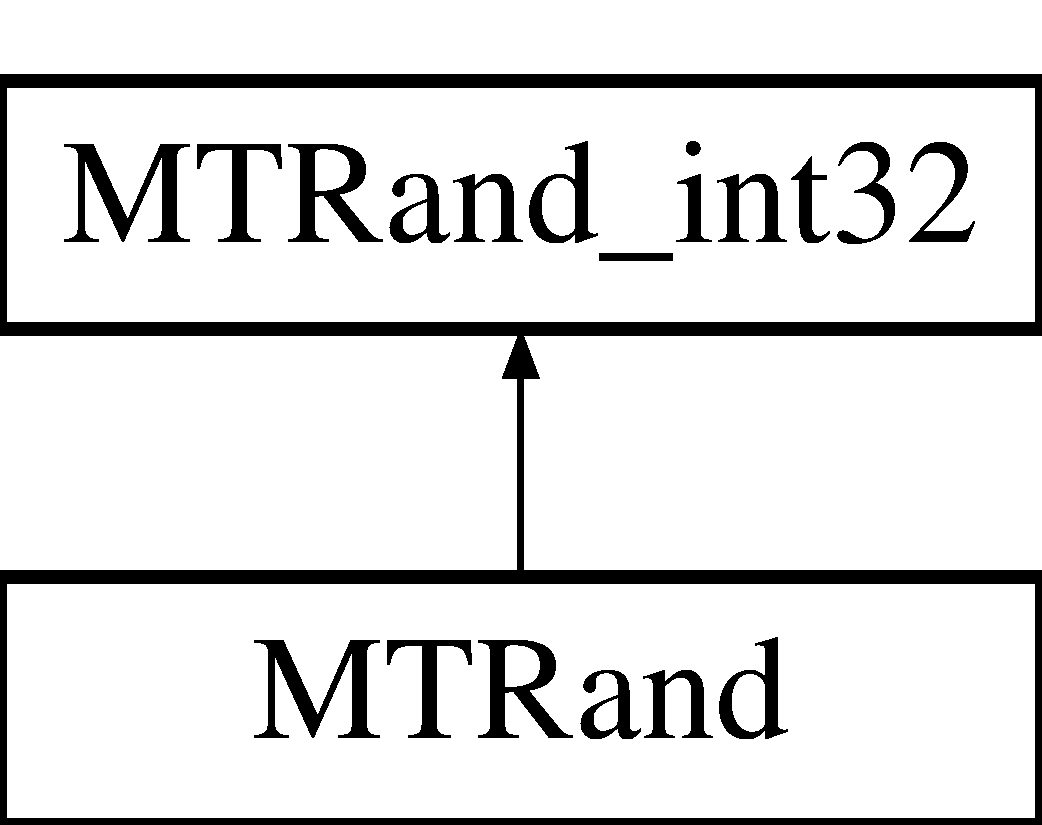
\includegraphics[height=2.000000cm]{class_m_t_rand}
\end{center}
\end{figure}
\subsection*{Public Member Functions}
\begin{DoxyCompactItemize}
\item 
\hyperlink{class_m_t_rand_a265dc65546e26073c0d5f8787b045a1d}{M\-T\-Rand} ()
\item 
\hyperlink{class_m_t_rand_a2c88736896bcbdb54bcdd7a0026720d5}{M\-T\-Rand} (unsigned long \hyperlink{class_m_t_rand__int32_a0c57076fe30358e0700a7ce1baa0ea27}{seed})
\item 
\hyperlink{class_m_t_rand_a6075a3beacdfb8e4cf48d9fb56cc193a}{M\-T\-Rand} (const unsigned long $\ast$\hyperlink{class_m_t_rand__int32_a0c57076fe30358e0700a7ce1baa0ea27}{seed}, int \hyperlink{crea__e__controlla__i__catalizzatori_8m_ae113ea7f9e515a12ac4b5595c6faf61e}{size})
\item 
\hyperlink{class_m_t_rand_a8c276546a41ae350dc9efc5e9c10a261}{$\sim$\-M\-T\-Rand} ()
\item 
double \hyperlink{class_m_t_rand_abbb87a08d622d58fdee0eea4cb5471a0}{operator()} ()
\end{DoxyCompactItemize}
\subsection*{Additional Inherited Members}


\subsection{Detailed Description}


Definition at line 97 of file mtrand.\-h.



\subsection{Constructor \& Destructor Documentation}
\hypertarget{class_m_t_rand_a265dc65546e26073c0d5f8787b045a1d}{\index{M\-T\-Rand@{M\-T\-Rand}!M\-T\-Rand@{M\-T\-Rand}}
\index{M\-T\-Rand@{M\-T\-Rand}!MTRand@{M\-T\-Rand}}
\subsubsection[{M\-T\-Rand}]{\setlength{\rightskip}{0pt plus 5cm}M\-T\-Rand\-::\-M\-T\-Rand (
\begin{DoxyParamCaption}
{}
\end{DoxyParamCaption}
)\hspace{0.3cm}{\ttfamily [inline]}}}\label{class_m_t_rand_a265dc65546e26073c0d5f8787b045a1d}


Definition at line 99 of file mtrand.\-h.

\hypertarget{class_m_t_rand_a2c88736896bcbdb54bcdd7a0026720d5}{\index{M\-T\-Rand@{M\-T\-Rand}!M\-T\-Rand@{M\-T\-Rand}}
\index{M\-T\-Rand@{M\-T\-Rand}!MTRand@{M\-T\-Rand}}
\subsubsection[{M\-T\-Rand}]{\setlength{\rightskip}{0pt plus 5cm}M\-T\-Rand\-::\-M\-T\-Rand (
\begin{DoxyParamCaption}
\item[{unsigned long}]{seed}
\end{DoxyParamCaption}
)\hspace{0.3cm}{\ttfamily [inline]}}}\label{class_m_t_rand_a2c88736896bcbdb54bcdd7a0026720d5}


Definition at line 100 of file mtrand.\-h.

\hypertarget{class_m_t_rand_a6075a3beacdfb8e4cf48d9fb56cc193a}{\index{M\-T\-Rand@{M\-T\-Rand}!M\-T\-Rand@{M\-T\-Rand}}
\index{M\-T\-Rand@{M\-T\-Rand}!MTRand@{M\-T\-Rand}}
\subsubsection[{M\-T\-Rand}]{\setlength{\rightskip}{0pt plus 5cm}M\-T\-Rand\-::\-M\-T\-Rand (
\begin{DoxyParamCaption}
\item[{const unsigned long $\ast$}]{seed, }
\item[{int}]{size}
\end{DoxyParamCaption}
)\hspace{0.3cm}{\ttfamily [inline]}}}\label{class_m_t_rand_a6075a3beacdfb8e4cf48d9fb56cc193a}


Definition at line 101 of file mtrand.\-h.

\hypertarget{class_m_t_rand_a8c276546a41ae350dc9efc5e9c10a261}{\index{M\-T\-Rand@{M\-T\-Rand}!$\sim$\-M\-T\-Rand@{$\sim$\-M\-T\-Rand}}
\index{$\sim$\-M\-T\-Rand@{$\sim$\-M\-T\-Rand}!MTRand@{M\-T\-Rand}}
\subsubsection[{$\sim$\-M\-T\-Rand}]{\setlength{\rightskip}{0pt plus 5cm}M\-T\-Rand\-::$\sim$\-M\-T\-Rand (
\begin{DoxyParamCaption}
{}
\end{DoxyParamCaption}
)\hspace{0.3cm}{\ttfamily [inline]}}}\label{class_m_t_rand_a8c276546a41ae350dc9efc5e9c10a261}


Definition at line 102 of file mtrand.\-h.



\subsection{Member Function Documentation}
\hypertarget{class_m_t_rand_abbb87a08d622d58fdee0eea4cb5471a0}{\index{M\-T\-Rand@{M\-T\-Rand}!operator()@{operator()}}
\index{operator()@{operator()}!MTRand@{M\-T\-Rand}}
\subsubsection[{operator()}]{\setlength{\rightskip}{0pt plus 5cm}double M\-T\-Rand\-::operator() (
\begin{DoxyParamCaption}
{}
\end{DoxyParamCaption}
)\hspace{0.3cm}{\ttfamily [inline]}}}\label{class_m_t_rand_abbb87a08d622d58fdee0eea4cb5471a0}


Definition at line 103 of file mtrand.\-h.



The documentation for this class was generated from the following file\-:\begin{DoxyCompactItemize}
\item 
/\-Users/alessandrofilisetti/\-Documents/\-G\-I\-T/carness/\hyperlink{mtrand_8h}{mtrand.\-h}\end{DoxyCompactItemize}

\hypertarget{class_m_t_rand53}{\section{M\-T\-Rand53 Class Reference}
\label{class_m_t_rand53}\index{M\-T\-Rand53@{M\-T\-Rand53}}
}


{\ttfamily \#include $<$mtrand.\-h$>$}

Inheritance diagram for M\-T\-Rand53\-:\begin{figure}[H]
\begin{center}
\leavevmode
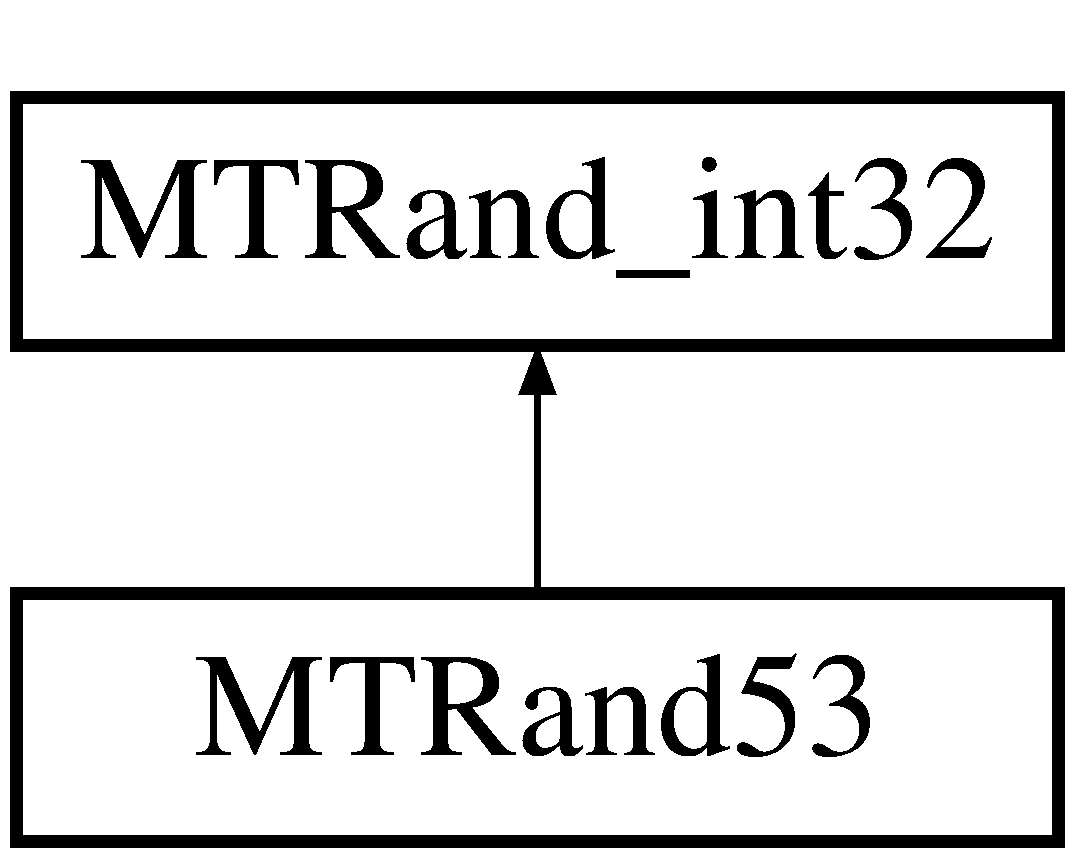
\includegraphics[height=2.000000cm]{class_m_t_rand53}
\end{center}
\end{figure}
\subsection*{Public Member Functions}
\begin{DoxyCompactItemize}
\item 
\hyperlink{class_m_t_rand53_a24711c9e6e5ee72715f34515d1f1939a}{M\-T\-Rand53} ()
\item 
\hyperlink{class_m_t_rand53_ad800887e15d4095f22facdb67f270c5e}{M\-T\-Rand53} (unsigned long \hyperlink{class_m_t_rand__int32_a0c57076fe30358e0700a7ce1baa0ea27}{seed})
\item 
\hyperlink{class_m_t_rand53_ac77b190d3ac27adea2d2c6c2ce2347c3}{M\-T\-Rand53} (const unsigned long $\ast$\hyperlink{class_m_t_rand__int32_a0c57076fe30358e0700a7ce1baa0ea27}{seed}, int \hyperlink{crea__e__controlla__i__catalizzatori_8m_ae113ea7f9e515a12ac4b5595c6faf61e}{size})
\item 
\hyperlink{class_m_t_rand53_a947a6a7afd0c8a17612cda3faa705a75}{$\sim$\-M\-T\-Rand53} ()
\item 
double \hyperlink{class_m_t_rand53_ab6657cb5349f39bc4553d3a970458b45}{operator()} ()
\end{DoxyCompactItemize}
\subsection*{Additional Inherited Members}


\subsection{Detailed Description}


Definition at line 139 of file mtrand.\-h.



\subsection{Constructor \& Destructor Documentation}
\hypertarget{class_m_t_rand53_a24711c9e6e5ee72715f34515d1f1939a}{\index{M\-T\-Rand53@{M\-T\-Rand53}!M\-T\-Rand53@{M\-T\-Rand53}}
\index{M\-T\-Rand53@{M\-T\-Rand53}!MTRand53@{M\-T\-Rand53}}
\subsubsection[{M\-T\-Rand53}]{\setlength{\rightskip}{0pt plus 5cm}M\-T\-Rand53\-::\-M\-T\-Rand53 (
\begin{DoxyParamCaption}
{}
\end{DoxyParamCaption}
)\hspace{0.3cm}{\ttfamily [inline]}}}\label{class_m_t_rand53_a24711c9e6e5ee72715f34515d1f1939a}


Definition at line 141 of file mtrand.\-h.

\hypertarget{class_m_t_rand53_ad800887e15d4095f22facdb67f270c5e}{\index{M\-T\-Rand53@{M\-T\-Rand53}!M\-T\-Rand53@{M\-T\-Rand53}}
\index{M\-T\-Rand53@{M\-T\-Rand53}!MTRand53@{M\-T\-Rand53}}
\subsubsection[{M\-T\-Rand53}]{\setlength{\rightskip}{0pt plus 5cm}M\-T\-Rand53\-::\-M\-T\-Rand53 (
\begin{DoxyParamCaption}
\item[{unsigned long}]{seed}
\end{DoxyParamCaption}
)\hspace{0.3cm}{\ttfamily [inline]}}}\label{class_m_t_rand53_ad800887e15d4095f22facdb67f270c5e}


Definition at line 142 of file mtrand.\-h.

\hypertarget{class_m_t_rand53_ac77b190d3ac27adea2d2c6c2ce2347c3}{\index{M\-T\-Rand53@{M\-T\-Rand53}!M\-T\-Rand53@{M\-T\-Rand53}}
\index{M\-T\-Rand53@{M\-T\-Rand53}!MTRand53@{M\-T\-Rand53}}
\subsubsection[{M\-T\-Rand53}]{\setlength{\rightskip}{0pt plus 5cm}M\-T\-Rand53\-::\-M\-T\-Rand53 (
\begin{DoxyParamCaption}
\item[{const unsigned long $\ast$}]{seed, }
\item[{int}]{size}
\end{DoxyParamCaption}
)\hspace{0.3cm}{\ttfamily [inline]}}}\label{class_m_t_rand53_ac77b190d3ac27adea2d2c6c2ce2347c3}


Definition at line 143 of file mtrand.\-h.

\hypertarget{class_m_t_rand53_a947a6a7afd0c8a17612cda3faa705a75}{\index{M\-T\-Rand53@{M\-T\-Rand53}!$\sim$\-M\-T\-Rand53@{$\sim$\-M\-T\-Rand53}}
\index{$\sim$\-M\-T\-Rand53@{$\sim$\-M\-T\-Rand53}!MTRand53@{M\-T\-Rand53}}
\subsubsection[{$\sim$\-M\-T\-Rand53}]{\setlength{\rightskip}{0pt plus 5cm}M\-T\-Rand53\-::$\sim$\-M\-T\-Rand53 (
\begin{DoxyParamCaption}
{}
\end{DoxyParamCaption}
)\hspace{0.3cm}{\ttfamily [inline]}}}\label{class_m_t_rand53_a947a6a7afd0c8a17612cda3faa705a75}


Definition at line 144 of file mtrand.\-h.



\subsection{Member Function Documentation}
\hypertarget{class_m_t_rand53_ab6657cb5349f39bc4553d3a970458b45}{\index{M\-T\-Rand53@{M\-T\-Rand53}!operator()@{operator()}}
\index{operator()@{operator()}!MTRand53@{M\-T\-Rand53}}
\subsubsection[{operator()}]{\setlength{\rightskip}{0pt plus 5cm}double M\-T\-Rand53\-::operator() (
\begin{DoxyParamCaption}
{}
\end{DoxyParamCaption}
)\hspace{0.3cm}{\ttfamily [inline]}}}\label{class_m_t_rand53_ab6657cb5349f39bc4553d3a970458b45}


Definition at line 145 of file mtrand.\-h.



The documentation for this class was generated from the following file\-:\begin{DoxyCompactItemize}
\item 
/\-Users/alessandrofilisetti/\-Dropbox/\-A\-C\-S\-\_\-\-S\-V\-N/carness/carness\-\_\-simulator/\hyperlink{mtrand_8h}{mtrand.\-h}\end{DoxyCompactItemize}

\hypertarget{class_m_t_rand__closed}{\section{M\-T\-Rand\-\_\-closed Class Reference}
\label{class_m_t_rand__closed}\index{M\-T\-Rand\-\_\-closed@{M\-T\-Rand\-\_\-closed}}
}


{\ttfamily \#include $<$mtrand.\-h$>$}

Inheritance diagram for M\-T\-Rand\-\_\-closed\-:\begin{figure}[H]
\begin{center}
\leavevmode
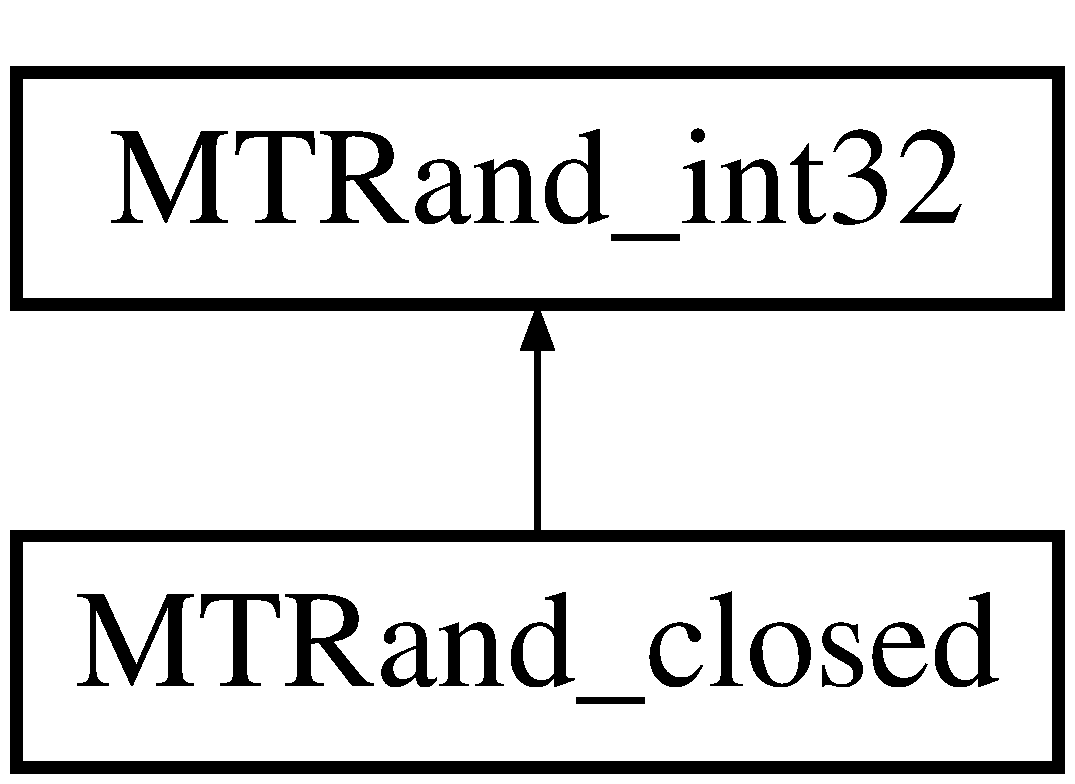
\includegraphics[height=2.000000cm]{class_m_t_rand__closed}
\end{center}
\end{figure}
\subsection*{Public Member Functions}
\begin{DoxyCompactItemize}
\item 
\hyperlink{class_m_t_rand__closed_a09b3b21b3cb35d04f2b6c290a817b2e8}{M\-T\-Rand\-\_\-closed} ()
\item 
\hyperlink{class_m_t_rand__closed_ad5dc83250b16f22d4693a18b51816271}{M\-T\-Rand\-\_\-closed} (unsigned long \hyperlink{class_m_t_rand__int32_a0c57076fe30358e0700a7ce1baa0ea27}{seed})
\item 
\hyperlink{class_m_t_rand__closed_a37e322f97253b7013823a267bcfe82d1}{M\-T\-Rand\-\_\-closed} (const unsigned long $\ast$\hyperlink{class_m_t_rand__int32_a0c57076fe30358e0700a7ce1baa0ea27}{seed}, int \hyperlink{crea__e__controlla__i__catalizzatori_8m_ae113ea7f9e515a12ac4b5595c6faf61e}{size})
\item 
\hyperlink{class_m_t_rand__closed_a46567ee841b5f54b305ac051ac837a8c}{$\sim$\-M\-T\-Rand\-\_\-closed} ()
\item 
double \hyperlink{class_m_t_rand__closed_ad0c535263b63c95029523183f672f62d}{operator()} ()
\end{DoxyCompactItemize}
\subsection*{Additional Inherited Members}


\subsection{Detailed Description}


Definition at line 111 of file mtrand.\-h.



\subsection{Constructor \& Destructor Documentation}
\hypertarget{class_m_t_rand__closed_a09b3b21b3cb35d04f2b6c290a817b2e8}{\index{M\-T\-Rand\-\_\-closed@{M\-T\-Rand\-\_\-closed}!M\-T\-Rand\-\_\-closed@{M\-T\-Rand\-\_\-closed}}
\index{M\-T\-Rand\-\_\-closed@{M\-T\-Rand\-\_\-closed}!MTRand_closed@{M\-T\-Rand\-\_\-closed}}
\subsubsection[{M\-T\-Rand\-\_\-closed}]{\setlength{\rightskip}{0pt plus 5cm}M\-T\-Rand\-\_\-closed\-::\-M\-T\-Rand\-\_\-closed (
\begin{DoxyParamCaption}
{}
\end{DoxyParamCaption}
)\hspace{0.3cm}{\ttfamily [inline]}}}\label{class_m_t_rand__closed_a09b3b21b3cb35d04f2b6c290a817b2e8}


Definition at line 113 of file mtrand.\-h.

\hypertarget{class_m_t_rand__closed_ad5dc83250b16f22d4693a18b51816271}{\index{M\-T\-Rand\-\_\-closed@{M\-T\-Rand\-\_\-closed}!M\-T\-Rand\-\_\-closed@{M\-T\-Rand\-\_\-closed}}
\index{M\-T\-Rand\-\_\-closed@{M\-T\-Rand\-\_\-closed}!MTRand_closed@{M\-T\-Rand\-\_\-closed}}
\subsubsection[{M\-T\-Rand\-\_\-closed}]{\setlength{\rightskip}{0pt plus 5cm}M\-T\-Rand\-\_\-closed\-::\-M\-T\-Rand\-\_\-closed (
\begin{DoxyParamCaption}
\item[{unsigned long}]{seed}
\end{DoxyParamCaption}
)\hspace{0.3cm}{\ttfamily [inline]}}}\label{class_m_t_rand__closed_ad5dc83250b16f22d4693a18b51816271}


Definition at line 114 of file mtrand.\-h.

\hypertarget{class_m_t_rand__closed_a37e322f97253b7013823a267bcfe82d1}{\index{M\-T\-Rand\-\_\-closed@{M\-T\-Rand\-\_\-closed}!M\-T\-Rand\-\_\-closed@{M\-T\-Rand\-\_\-closed}}
\index{M\-T\-Rand\-\_\-closed@{M\-T\-Rand\-\_\-closed}!MTRand_closed@{M\-T\-Rand\-\_\-closed}}
\subsubsection[{M\-T\-Rand\-\_\-closed}]{\setlength{\rightskip}{0pt plus 5cm}M\-T\-Rand\-\_\-closed\-::\-M\-T\-Rand\-\_\-closed (
\begin{DoxyParamCaption}
\item[{const unsigned long $\ast$}]{seed, }
\item[{int}]{size}
\end{DoxyParamCaption}
)\hspace{0.3cm}{\ttfamily [inline]}}}\label{class_m_t_rand__closed_a37e322f97253b7013823a267bcfe82d1}


Definition at line 115 of file mtrand.\-h.

\hypertarget{class_m_t_rand__closed_a46567ee841b5f54b305ac051ac837a8c}{\index{M\-T\-Rand\-\_\-closed@{M\-T\-Rand\-\_\-closed}!$\sim$\-M\-T\-Rand\-\_\-closed@{$\sim$\-M\-T\-Rand\-\_\-closed}}
\index{$\sim$\-M\-T\-Rand\-\_\-closed@{$\sim$\-M\-T\-Rand\-\_\-closed}!MTRand_closed@{M\-T\-Rand\-\_\-closed}}
\subsubsection[{$\sim$\-M\-T\-Rand\-\_\-closed}]{\setlength{\rightskip}{0pt plus 5cm}M\-T\-Rand\-\_\-closed\-::$\sim$\-M\-T\-Rand\-\_\-closed (
\begin{DoxyParamCaption}
{}
\end{DoxyParamCaption}
)\hspace{0.3cm}{\ttfamily [inline]}}}\label{class_m_t_rand__closed_a46567ee841b5f54b305ac051ac837a8c}


Definition at line 116 of file mtrand.\-h.



\subsection{Member Function Documentation}
\hypertarget{class_m_t_rand__closed_ad0c535263b63c95029523183f672f62d}{\index{M\-T\-Rand\-\_\-closed@{M\-T\-Rand\-\_\-closed}!operator()@{operator()}}
\index{operator()@{operator()}!MTRand_closed@{M\-T\-Rand\-\_\-closed}}
\subsubsection[{operator()}]{\setlength{\rightskip}{0pt plus 5cm}double M\-T\-Rand\-\_\-closed\-::operator() (
\begin{DoxyParamCaption}
{}
\end{DoxyParamCaption}
)\hspace{0.3cm}{\ttfamily [inline]}}}\label{class_m_t_rand__closed_ad0c535263b63c95029523183f672f62d}


Definition at line 117 of file mtrand.\-h.



The documentation for this class was generated from the following file\-:\begin{DoxyCompactItemize}
\item 
/\-Users/alessandrofilisetti/\-Dropbox/\-A\-C\-S\-\_\-\-S\-V\-N/carness/carness\-\_\-simulator/\hyperlink{mtrand_8h}{mtrand.\-h}\end{DoxyCompactItemize}

\hypertarget{class_m_t_rand__int32}{\section{M\-T\-Rand\-\_\-int32 Class Reference}
\label{class_m_t_rand__int32}\index{M\-T\-Rand\-\_\-int32@{M\-T\-Rand\-\_\-int32}}
}


{\ttfamily \#include $<$mtrand.\-h$>$}

Inheritance diagram for M\-T\-Rand\-\_\-int32\-:\begin{figure}[H]
\begin{center}
\leavevmode
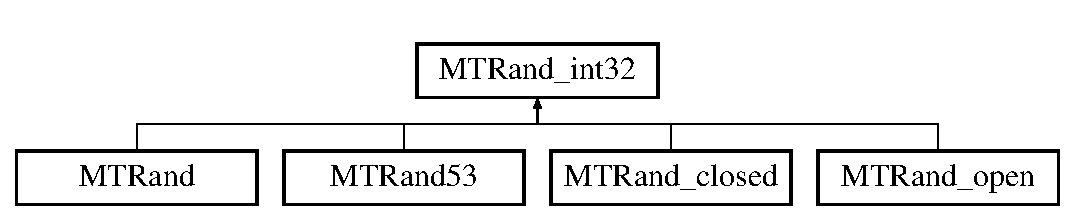
\includegraphics[height=2.000000cm]{class_m_t_rand__int32}
\end{center}
\end{figure}
\subsection*{Public Member Functions}
\begin{DoxyCompactItemize}
\item 
\hyperlink{class_m_t_rand__int32_a034f223c086f5368bd220b02f2cc12a8}{M\-T\-Rand\-\_\-int32} ()
\item 
\hyperlink{class_m_t_rand__int32_ad30f7c63a6f1fb3c3b76b8ce6ffa0206}{M\-T\-Rand\-\_\-int32} (unsigned long s)
\item 
\hyperlink{class_m_t_rand__int32_a19acddb3910a7282517b2ffc398b92b4}{M\-T\-Rand\-\_\-int32} (const unsigned long $\ast$array, int \hyperlink{crea__e__controlla__i__catalizzatori_8m_ae113ea7f9e515a12ac4b5595c6faf61e}{size})
\item 
void \hyperlink{class_m_t_rand__int32_a0c57076fe30358e0700a7ce1baa0ea27}{seed} (unsigned long)
\item 
void \hyperlink{class_m_t_rand__int32_a3cabc1e3445716236a570ffd2f69686d}{seed} (const unsigned long $\ast$, int \hyperlink{crea__e__controlla__i__catalizzatori_8m_ae113ea7f9e515a12ac4b5595c6faf61e}{size})
\item 
unsigned long \hyperlink{class_m_t_rand__int32_ad7fe22190d0411c6dac8e6f471633aa4}{operator()} ()
\item 
virtual \hyperlink{class_m_t_rand__int32_a364900abea0758d070ce89922159923a}{$\sim$\-M\-T\-Rand\-\_\-int32} ()
\end{DoxyCompactItemize}
\subsection*{Protected Member Functions}
\begin{DoxyCompactItemize}
\item 
unsigned long \hyperlink{class_m_t_rand__int32_abacdfa346255baeac69d29bb57f29b22}{rand\-\_\-int32} ()
\end{DoxyCompactItemize}


\subsection{Detailed Description}


Definition at line 48 of file mtrand.\-h.



\subsection{Constructor \& Destructor Documentation}
\hypertarget{class_m_t_rand__int32_a034f223c086f5368bd220b02f2cc12a8}{\index{M\-T\-Rand\-\_\-int32@{M\-T\-Rand\-\_\-int32}!M\-T\-Rand\-\_\-int32@{M\-T\-Rand\-\_\-int32}}
\index{M\-T\-Rand\-\_\-int32@{M\-T\-Rand\-\_\-int32}!MTRand_int32@{M\-T\-Rand\-\_\-int32}}
\subsubsection[{M\-T\-Rand\-\_\-int32}]{\setlength{\rightskip}{0pt plus 5cm}M\-T\-Rand\-\_\-int32\-::\-M\-T\-Rand\-\_\-int32 (
\begin{DoxyParamCaption}
{}
\end{DoxyParamCaption}
)\hspace{0.3cm}{\ttfamily [inline]}}}\label{class_m_t_rand__int32_a034f223c086f5368bd220b02f2cc12a8}


Definition at line 51 of file mtrand.\-h.

\hypertarget{class_m_t_rand__int32_ad30f7c63a6f1fb3c3b76b8ce6ffa0206}{\index{M\-T\-Rand\-\_\-int32@{M\-T\-Rand\-\_\-int32}!M\-T\-Rand\-\_\-int32@{M\-T\-Rand\-\_\-int32}}
\index{M\-T\-Rand\-\_\-int32@{M\-T\-Rand\-\_\-int32}!MTRand_int32@{M\-T\-Rand\-\_\-int32}}
\subsubsection[{M\-T\-Rand\-\_\-int32}]{\setlength{\rightskip}{0pt plus 5cm}M\-T\-Rand\-\_\-int32\-::\-M\-T\-Rand\-\_\-int32 (
\begin{DoxyParamCaption}
\item[{unsigned long}]{s}
\end{DoxyParamCaption}
)\hspace{0.3cm}{\ttfamily [inline]}}}\label{class_m_t_rand__int32_ad30f7c63a6f1fb3c3b76b8ce6ffa0206}


Definition at line 53 of file mtrand.\-h.

\hypertarget{class_m_t_rand__int32_a19acddb3910a7282517b2ffc398b92b4}{\index{M\-T\-Rand\-\_\-int32@{M\-T\-Rand\-\_\-int32}!M\-T\-Rand\-\_\-int32@{M\-T\-Rand\-\_\-int32}}
\index{M\-T\-Rand\-\_\-int32@{M\-T\-Rand\-\_\-int32}!MTRand_int32@{M\-T\-Rand\-\_\-int32}}
\subsubsection[{M\-T\-Rand\-\_\-int32}]{\setlength{\rightskip}{0pt plus 5cm}M\-T\-Rand\-\_\-int32\-::\-M\-T\-Rand\-\_\-int32 (
\begin{DoxyParamCaption}
\item[{const unsigned long $\ast$}]{array, }
\item[{int}]{size}
\end{DoxyParamCaption}
)\hspace{0.3cm}{\ttfamily [inline]}}}\label{class_m_t_rand__int32_a19acddb3910a7282517b2ffc398b92b4}


Definition at line 55 of file mtrand.\-h.

\hypertarget{class_m_t_rand__int32_a364900abea0758d070ce89922159923a}{\index{M\-T\-Rand\-\_\-int32@{M\-T\-Rand\-\_\-int32}!$\sim$\-M\-T\-Rand\-\_\-int32@{$\sim$\-M\-T\-Rand\-\_\-int32}}
\index{$\sim$\-M\-T\-Rand\-\_\-int32@{$\sim$\-M\-T\-Rand\-\_\-int32}!MTRand_int32@{M\-T\-Rand\-\_\-int32}}
\subsubsection[{$\sim$\-M\-T\-Rand\-\_\-int32}]{\setlength{\rightskip}{0pt plus 5cm}virtual M\-T\-Rand\-\_\-int32\-::$\sim$\-M\-T\-Rand\-\_\-int32 (
\begin{DoxyParamCaption}
{}
\end{DoxyParamCaption}
)\hspace{0.3cm}{\ttfamily [inline]}, {\ttfamily [virtual]}}}\label{class_m_t_rand__int32_a364900abea0758d070ce89922159923a}


Definition at line 62 of file mtrand.\-h.



\subsection{Member Function Documentation}
\hypertarget{class_m_t_rand__int32_ad7fe22190d0411c6dac8e6f471633aa4}{\index{M\-T\-Rand\-\_\-int32@{M\-T\-Rand\-\_\-int32}!operator()@{operator()}}
\index{operator()@{operator()}!MTRand_int32@{M\-T\-Rand\-\_\-int32}}
\subsubsection[{operator()}]{\setlength{\rightskip}{0pt plus 5cm}unsigned long M\-T\-Rand\-\_\-int32\-::operator() (
\begin{DoxyParamCaption}
{}
\end{DoxyParamCaption}
)\hspace{0.3cm}{\ttfamily [inline]}}}\label{class_m_t_rand__int32_ad7fe22190d0411c6dac8e6f471633aa4}


Definition at line 60 of file mtrand.\-h.

\hypertarget{class_m_t_rand__int32_abacdfa346255baeac69d29bb57f29b22}{\index{M\-T\-Rand\-\_\-int32@{M\-T\-Rand\-\_\-int32}!rand\-\_\-int32@{rand\-\_\-int32}}
\index{rand\-\_\-int32@{rand\-\_\-int32}!MTRand_int32@{M\-T\-Rand\-\_\-int32}}
\subsubsection[{rand\-\_\-int32}]{\setlength{\rightskip}{0pt plus 5cm}unsigned long M\-T\-Rand\-\_\-int32\-::rand\-\_\-int32 (
\begin{DoxyParamCaption}
{}
\end{DoxyParamCaption}
)\hspace{0.3cm}{\ttfamily [inline]}, {\ttfamily [protected]}}}\label{class_m_t_rand__int32_abacdfa346255baeac69d29bb57f29b22}


Definition at line 85 of file mtrand.\-h.

\hypertarget{class_m_t_rand__int32_a0c57076fe30358e0700a7ce1baa0ea27}{\index{M\-T\-Rand\-\_\-int32@{M\-T\-Rand\-\_\-int32}!seed@{seed}}
\index{seed@{seed}!MTRand_int32@{M\-T\-Rand\-\_\-int32}}
\subsubsection[{seed}]{\setlength{\rightskip}{0pt plus 5cm}void M\-T\-Rand\-\_\-int32\-::seed (
\begin{DoxyParamCaption}
\item[{unsigned long}]{s}
\end{DoxyParamCaption}
)}}\label{class_m_t_rand__int32_a0c57076fe30358e0700a7ce1baa0ea27}


Definition at line 23 of file mtrand.\-cpp.

\hypertarget{class_m_t_rand__int32_a3cabc1e3445716236a570ffd2f69686d}{\index{M\-T\-Rand\-\_\-int32@{M\-T\-Rand\-\_\-int32}!seed@{seed}}
\index{seed@{seed}!MTRand_int32@{M\-T\-Rand\-\_\-int32}}
\subsubsection[{seed}]{\setlength{\rightskip}{0pt plus 5cm}void M\-T\-Rand\-\_\-int32\-::seed (
\begin{DoxyParamCaption}
\item[{const unsigned long $\ast$}]{array, }
\item[{int}]{size}
\end{DoxyParamCaption}
)}}\label{class_m_t_rand__int32_a3cabc1e3445716236a570ffd2f69686d}


Definition at line 35 of file mtrand.\-cpp.



The documentation for this class was generated from the following files\-:\begin{DoxyCompactItemize}
\item 
/\-Users/alessandrofilisetti/\-Dropbox/\-A\-C\-S\-\_\-\-S\-V\-N/carness/carness\-\_\-simulator/\hyperlink{mtrand_8h}{mtrand.\-h}\item 
/\-Users/alessandrofilisetti/\-Dropbox/\-A\-C\-S\-\_\-\-S\-V\-N/carness/carness\-\_\-simulator/\hyperlink{mtrand_8cpp}{mtrand.\-cpp}\end{DoxyCompactItemize}

\hypertarget{class_m_t_rand__open}{\section{M\-T\-Rand\-\_\-open Class Reference}
\label{class_m_t_rand__open}\index{M\-T\-Rand\-\_\-open@{M\-T\-Rand\-\_\-open}}
}


{\ttfamily \#include $<$mtrand.\-h$>$}

Inheritance diagram for M\-T\-Rand\-\_\-open\-:\begin{figure}[H]
\begin{center}
\leavevmode
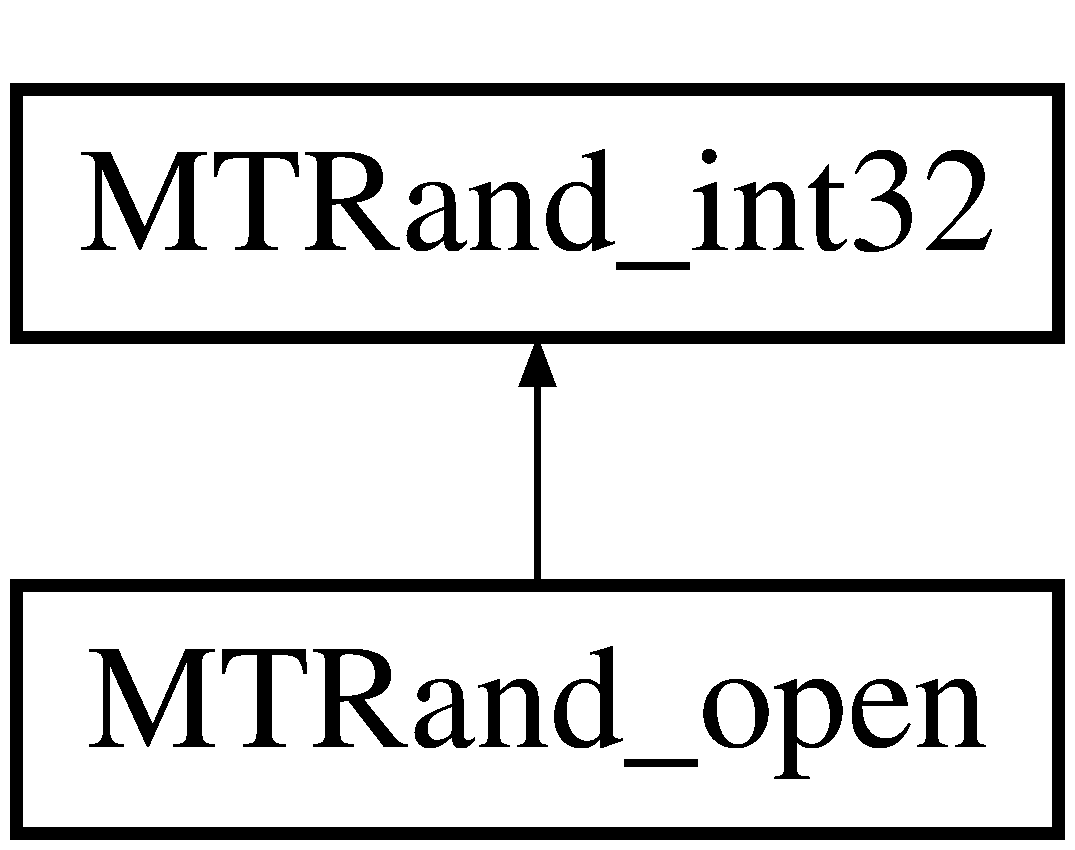
\includegraphics[height=2.000000cm]{class_m_t_rand__open}
\end{center}
\end{figure}
\subsection*{Public Member Functions}
\begin{DoxyCompactItemize}
\item 
\hyperlink{class_m_t_rand__open_a58140b54564be39382da163954177389}{M\-T\-Rand\-\_\-open} ()
\item 
\hyperlink{class_m_t_rand__open_a1f55ebc1052f5343f8d6e08a752ef957}{M\-T\-Rand\-\_\-open} (unsigned long \hyperlink{class_m_t_rand__int32_a0c57076fe30358e0700a7ce1baa0ea27}{seed})
\item 
\hyperlink{class_m_t_rand__open_a0216992f4dfa5acf22ee8c585eeac488}{M\-T\-Rand\-\_\-open} (const unsigned long $\ast$\hyperlink{class_m_t_rand__int32_a0c57076fe30358e0700a7ce1baa0ea27}{seed}, int \hyperlink{crea__e__controlla__i__catalizzatori_8m_ae113ea7f9e515a12ac4b5595c6faf61e}{size})
\item 
\hyperlink{class_m_t_rand__open_a4f4774b5d9b79972dedaec984b248581}{$\sim$\-M\-T\-Rand\-\_\-open} ()
\item 
double \hyperlink{class_m_t_rand__open_ac408aa400ca59fc2afc888d88f98d807}{operator()} ()
\end{DoxyCompactItemize}
\subsection*{Additional Inherited Members}


\subsection{Detailed Description}


Definition at line 125 of file mtrand.\-h.



\subsection{Constructor \& Destructor Documentation}
\hypertarget{class_m_t_rand__open_a58140b54564be39382da163954177389}{\index{M\-T\-Rand\-\_\-open@{M\-T\-Rand\-\_\-open}!M\-T\-Rand\-\_\-open@{M\-T\-Rand\-\_\-open}}
\index{M\-T\-Rand\-\_\-open@{M\-T\-Rand\-\_\-open}!MTRand_open@{M\-T\-Rand\-\_\-open}}
\subsubsection[{M\-T\-Rand\-\_\-open}]{\setlength{\rightskip}{0pt plus 5cm}M\-T\-Rand\-\_\-open\-::\-M\-T\-Rand\-\_\-open (
\begin{DoxyParamCaption}
{}
\end{DoxyParamCaption}
)\hspace{0.3cm}{\ttfamily [inline]}}}\label{class_m_t_rand__open_a58140b54564be39382da163954177389}


Definition at line 127 of file mtrand.\-h.

\hypertarget{class_m_t_rand__open_a1f55ebc1052f5343f8d6e08a752ef957}{\index{M\-T\-Rand\-\_\-open@{M\-T\-Rand\-\_\-open}!M\-T\-Rand\-\_\-open@{M\-T\-Rand\-\_\-open}}
\index{M\-T\-Rand\-\_\-open@{M\-T\-Rand\-\_\-open}!MTRand_open@{M\-T\-Rand\-\_\-open}}
\subsubsection[{M\-T\-Rand\-\_\-open}]{\setlength{\rightskip}{0pt plus 5cm}M\-T\-Rand\-\_\-open\-::\-M\-T\-Rand\-\_\-open (
\begin{DoxyParamCaption}
\item[{unsigned long}]{seed}
\end{DoxyParamCaption}
)\hspace{0.3cm}{\ttfamily [inline]}}}\label{class_m_t_rand__open_a1f55ebc1052f5343f8d6e08a752ef957}


Definition at line 128 of file mtrand.\-h.

\hypertarget{class_m_t_rand__open_a0216992f4dfa5acf22ee8c585eeac488}{\index{M\-T\-Rand\-\_\-open@{M\-T\-Rand\-\_\-open}!M\-T\-Rand\-\_\-open@{M\-T\-Rand\-\_\-open}}
\index{M\-T\-Rand\-\_\-open@{M\-T\-Rand\-\_\-open}!MTRand_open@{M\-T\-Rand\-\_\-open}}
\subsubsection[{M\-T\-Rand\-\_\-open}]{\setlength{\rightskip}{0pt plus 5cm}M\-T\-Rand\-\_\-open\-::\-M\-T\-Rand\-\_\-open (
\begin{DoxyParamCaption}
\item[{const unsigned long $\ast$}]{seed, }
\item[{int}]{size}
\end{DoxyParamCaption}
)\hspace{0.3cm}{\ttfamily [inline]}}}\label{class_m_t_rand__open_a0216992f4dfa5acf22ee8c585eeac488}


Definition at line 129 of file mtrand.\-h.

\hypertarget{class_m_t_rand__open_a4f4774b5d9b79972dedaec984b248581}{\index{M\-T\-Rand\-\_\-open@{M\-T\-Rand\-\_\-open}!$\sim$\-M\-T\-Rand\-\_\-open@{$\sim$\-M\-T\-Rand\-\_\-open}}
\index{$\sim$\-M\-T\-Rand\-\_\-open@{$\sim$\-M\-T\-Rand\-\_\-open}!MTRand_open@{M\-T\-Rand\-\_\-open}}
\subsubsection[{$\sim$\-M\-T\-Rand\-\_\-open}]{\setlength{\rightskip}{0pt plus 5cm}M\-T\-Rand\-\_\-open\-::$\sim$\-M\-T\-Rand\-\_\-open (
\begin{DoxyParamCaption}
{}
\end{DoxyParamCaption}
)\hspace{0.3cm}{\ttfamily [inline]}}}\label{class_m_t_rand__open_a4f4774b5d9b79972dedaec984b248581}


Definition at line 130 of file mtrand.\-h.



\subsection{Member Function Documentation}
\hypertarget{class_m_t_rand__open_ac408aa400ca59fc2afc888d88f98d807}{\index{M\-T\-Rand\-\_\-open@{M\-T\-Rand\-\_\-open}!operator()@{operator()}}
\index{operator()@{operator()}!MTRand_open@{M\-T\-Rand\-\_\-open}}
\subsubsection[{operator()}]{\setlength{\rightskip}{0pt plus 5cm}double M\-T\-Rand\-\_\-open\-::operator() (
\begin{DoxyParamCaption}
{}
\end{DoxyParamCaption}
)\hspace{0.3cm}{\ttfamily [inline]}}}\label{class_m_t_rand__open_ac408aa400ca59fc2afc888d88f98d807}


Definition at line 131 of file mtrand.\-h.



The documentation for this class was generated from the following file\-:\begin{DoxyCompactItemize}
\item 
/\-Users/alessandrofilisetti/\-Dropbox/\-A\-C\-S\-\_\-\-S\-V\-N/carness/carness\-\_\-simulator/\hyperlink{mtrand_8h}{mtrand.\-h}\end{DoxyCompactItemize}

\hypertarget{classreactions}{\section{reactions Class Reference}
\label{classreactions}\index{reactions@{reactions}}
}


{\ttfamily \#include $<$reactions.\-h$>$}

\subsection*{Public Member Functions}
\begin{DoxyCompactItemize}
\item 
\hyperlink{classreactions_a496de9cbc128b98213ded20b936752c2}{reactions} (\hyperlink{acs__headers_8h_a19319d75f02db4308bc5c0026d98cd85}{acs\-\_\-long\-Int} tmp\-I\-D, \hyperlink{acs__headers_8h_a8d277355641a098190360234e2ebde35}{acs\-\_\-int} tmp\-Type, \hyperlink{acs__headers_8h_a19319d75f02db4308bc5c0026d98cd85}{acs\-\_\-long\-Int} tmp\-M\-\_\-\-I, \hyperlink{acs__headers_8h_a19319d75f02db4308bc5c0026d98cd85}{acs\-\_\-long\-Int} tmp\-M\-\_\-\-I\-I, \hyperlink{acs__headers_8h_a19319d75f02db4308bc5c0026d98cd85}{acs\-\_\-long\-Int} tmp\-M\-\_\-\-I\-I\-I, \hyperlink{acs__headers_8h_a8d277355641a098190360234e2ebde35}{acs\-\_\-int} tmp\-Events, \hyperlink{acs__headers_8h_a8d277355641a098190360234e2ebde35}{acs\-\_\-int} tmp\-Energy\-Type)
\begin{DoxyCompactList}\small\item\em Constructor. \end{DoxyCompactList}\item 
\hyperlink{classreactions_ad0c79e56e87891c502d8fcd6c4005987}{$\sim$reactions} ()
\item 
\hyperlink{acs__headers_8h_a19319d75f02db4308bc5c0026d98cd85}{acs\-\_\-long\-Int} \hyperlink{classreactions_a5c30ce559254e67f7d4e219a8fe26fcc}{get\-I\-D} () const 
\item 
\hyperlink{acs__headers_8h_a8d277355641a098190360234e2ebde35}{acs\-\_\-int} \hyperlink{classreactions_ad928f8c901ad8e318e201cedcf1209ba}{get\-Type} () const 
\item 
\hyperlink{acs__headers_8h_a19319d75f02db4308bc5c0026d98cd85}{acs\-\_\-long\-Int} \hyperlink{classreactions_a90adbdb8288b8c67c7715949848583ab}{get\-Species\-\_\-\-I} () const 
\item 
\hyperlink{acs__headers_8h_a19319d75f02db4308bc5c0026d98cd85}{acs\-\_\-long\-Int} \hyperlink{classreactions_ac0bdd6d9081645bf3a2c5531a71cbe40}{get\-Species\-\_\-\-I\-I} () const 
\item 
\hyperlink{acs__headers_8h_a19319d75f02db4308bc5c0026d98cd85}{acs\-\_\-long\-Int} \hyperlink{classreactions_aaf426633019113ac4ae54cd5597920be}{get\-Species\-\_\-\-I\-I\-I} () const 
\item 
\hyperlink{acs__headers_8h_a8d277355641a098190360234e2ebde35}{acs\-\_\-int} \hyperlink{classreactions_a4fd82a3f1a6474e53709c2a8c04b793c}{get\-Events} () const 
\item 
\hyperlink{acs__headers_8h_a8d277355641a098190360234e2ebde35}{acs\-\_\-int} \hyperlink{classreactions_ae6fce196577644283fdab4a78909d891}{get\-Energy\-Type} () const 
\item 
void \hyperlink{classreactions_ae7a0bcb1c921c25ad5dc637d664f2c94}{update\-Tot\-Events} ()
\item 
void \hyperlink{classreactions_a614a367a15dda1df4160bcdc170a9b32}{reset\-Events\-Counter} ()
\end{DoxyCompactItemize}


\subsection{Detailed Description}


Definition at line 17 of file reactions.\-h.



\subsection{Constructor \& Destructor Documentation}
\hypertarget{classreactions_a496de9cbc128b98213ded20b936752c2}{\index{reactions@{reactions}!reactions@{reactions}}
\index{reactions@{reactions}!reactions@{reactions}}
\subsubsection[{reactions}]{\setlength{\rightskip}{0pt plus 5cm}reactions\-::reactions (
\begin{DoxyParamCaption}
\item[{{\bf acs\-\_\-long\-Int}}]{tmp\-I\-D, }
\item[{{\bf acs\-\_\-int}}]{tmp\-Type, }
\item[{{\bf acs\-\_\-long\-Int}}]{tmp\-M\-\_\-\-I, }
\item[{{\bf acs\-\_\-long\-Int}}]{tmp\-M\-\_\-\-I\-I, }
\item[{{\bf acs\-\_\-long\-Int}}]{tmp\-M\-\_\-\-I\-I\-I, }
\item[{{\bf acs\-\_\-int}}]{tmp\-Events, }
\item[{{\bf acs\-\_\-int}}]{tmp\-Energy\-Type}
\end{DoxyParamCaption}
)}}\label{classreactions_a496de9cbc128b98213ded20b936752c2}


Constructor. 


\begin{DoxyParams}{Parameters}
{\em tmp\-I\-D} & reaction identificator \\
\hline
{\em tmp\-Type} & condensation or cleavage \\
\hline
{\em tmp\-M\-\_\-\-I} & product (if condensation) or substrates (if cleavage) \\
\hline
{\em tmp\-M\-\_\-\-I\-I} & product (if cleavage) or substrates (if condensation) \\
\hline
{\em tmp\-M\-\_\-\-I\-I\-I} & product (if cleavage) or substrates (if condensation) \\
\hline
{\em tmp\-Keq} & equilibrium constant \\
\hline
\end{DoxyParams}


Definition at line 20 of file reactions.\-cpp.

\hypertarget{classreactions_ad0c79e56e87891c502d8fcd6c4005987}{\index{reactions@{reactions}!$\sim$reactions@{$\sim$reactions}}
\index{$\sim$reactions@{$\sim$reactions}!reactions@{reactions}}
\subsubsection[{$\sim$reactions}]{\setlength{\rightskip}{0pt plus 5cm}reactions\-::$\sim$reactions (
\begin{DoxyParamCaption}
{}
\end{DoxyParamCaption}
)\hspace{0.3cm}{\ttfamily [inline]}}}\label{classreactions_ad0c79e56e87891c502d8fcd6c4005987}


Definition at line 32 of file reactions.\-h.



\subsection{Member Function Documentation}
\hypertarget{classreactions_ae6fce196577644283fdab4a78909d891}{\index{reactions@{reactions}!get\-Energy\-Type@{get\-Energy\-Type}}
\index{get\-Energy\-Type@{get\-Energy\-Type}!reactions@{reactions}}
\subsubsection[{get\-Energy\-Type}]{\setlength{\rightskip}{0pt plus 5cm}{\bf acs\-\_\-int} reactions\-::get\-Energy\-Type (
\begin{DoxyParamCaption}
{}
\end{DoxyParamCaption}
) const\hspace{0.3cm}{\ttfamily [inline]}}}\label{classreactions_ae6fce196577644283fdab4a78909d891}


Definition at line 41 of file reactions.\-h.

\hypertarget{classreactions_a4fd82a3f1a6474e53709c2a8c04b793c}{\index{reactions@{reactions}!get\-Events@{get\-Events}}
\index{get\-Events@{get\-Events}!reactions@{reactions}}
\subsubsection[{get\-Events}]{\setlength{\rightskip}{0pt plus 5cm}{\bf acs\-\_\-int} reactions\-::get\-Events (
\begin{DoxyParamCaption}
{}
\end{DoxyParamCaption}
) const\hspace{0.3cm}{\ttfamily [inline]}}}\label{classreactions_a4fd82a3f1a6474e53709c2a8c04b793c}


Definition at line 40 of file reactions.\-h.

\hypertarget{classreactions_a5c30ce559254e67f7d4e219a8fe26fcc}{\index{reactions@{reactions}!get\-I\-D@{get\-I\-D}}
\index{get\-I\-D@{get\-I\-D}!reactions@{reactions}}
\subsubsection[{get\-I\-D}]{\setlength{\rightskip}{0pt plus 5cm}{\bf acs\-\_\-long\-Int} reactions\-::get\-I\-D (
\begin{DoxyParamCaption}
{}
\end{DoxyParamCaption}
) const\hspace{0.3cm}{\ttfamily [inline]}}}\label{classreactions_a5c30ce559254e67f7d4e219a8fe26fcc}


Definition at line 35 of file reactions.\-h.

\hypertarget{classreactions_a90adbdb8288b8c67c7715949848583ab}{\index{reactions@{reactions}!get\-Species\-\_\-\-I@{get\-Species\-\_\-\-I}}
\index{get\-Species\-\_\-\-I@{get\-Species\-\_\-\-I}!reactions@{reactions}}
\subsubsection[{get\-Species\-\_\-\-I}]{\setlength{\rightskip}{0pt plus 5cm}{\bf acs\-\_\-long\-Int} reactions\-::get\-Species\-\_\-\-I (
\begin{DoxyParamCaption}
{}
\end{DoxyParamCaption}
) const\hspace{0.3cm}{\ttfamily [inline]}}}\label{classreactions_a90adbdb8288b8c67c7715949848583ab}


Definition at line 37 of file reactions.\-h.

\hypertarget{classreactions_ac0bdd6d9081645bf3a2c5531a71cbe40}{\index{reactions@{reactions}!get\-Species\-\_\-\-I\-I@{get\-Species\-\_\-\-I\-I}}
\index{get\-Species\-\_\-\-I\-I@{get\-Species\-\_\-\-I\-I}!reactions@{reactions}}
\subsubsection[{get\-Species\-\_\-\-I\-I}]{\setlength{\rightskip}{0pt plus 5cm}{\bf acs\-\_\-long\-Int} reactions\-::get\-Species\-\_\-\-I\-I (
\begin{DoxyParamCaption}
{}
\end{DoxyParamCaption}
) const\hspace{0.3cm}{\ttfamily [inline]}}}\label{classreactions_ac0bdd6d9081645bf3a2c5531a71cbe40}


Definition at line 38 of file reactions.\-h.

\hypertarget{classreactions_aaf426633019113ac4ae54cd5597920be}{\index{reactions@{reactions}!get\-Species\-\_\-\-I\-I\-I@{get\-Species\-\_\-\-I\-I\-I}}
\index{get\-Species\-\_\-\-I\-I\-I@{get\-Species\-\_\-\-I\-I\-I}!reactions@{reactions}}
\subsubsection[{get\-Species\-\_\-\-I\-I\-I}]{\setlength{\rightskip}{0pt plus 5cm}{\bf acs\-\_\-long\-Int} reactions\-::get\-Species\-\_\-\-I\-I\-I (
\begin{DoxyParamCaption}
{}
\end{DoxyParamCaption}
) const\hspace{0.3cm}{\ttfamily [inline]}}}\label{classreactions_aaf426633019113ac4ae54cd5597920be}


Definition at line 39 of file reactions.\-h.

\hypertarget{classreactions_ad928f8c901ad8e318e201cedcf1209ba}{\index{reactions@{reactions}!get\-Type@{get\-Type}}
\index{get\-Type@{get\-Type}!reactions@{reactions}}
\subsubsection[{get\-Type}]{\setlength{\rightskip}{0pt plus 5cm}{\bf acs\-\_\-int} reactions\-::get\-Type (
\begin{DoxyParamCaption}
{}
\end{DoxyParamCaption}
) const\hspace{0.3cm}{\ttfamily [inline]}}}\label{classreactions_ad928f8c901ad8e318e201cedcf1209ba}


Definition at line 36 of file reactions.\-h.

\hypertarget{classreactions_a614a367a15dda1df4160bcdc170a9b32}{\index{reactions@{reactions}!reset\-Events\-Counter@{reset\-Events\-Counter}}
\index{reset\-Events\-Counter@{reset\-Events\-Counter}!reactions@{reactions}}
\subsubsection[{reset\-Events\-Counter}]{\setlength{\rightskip}{0pt plus 5cm}void reactions\-::reset\-Events\-Counter (
\begin{DoxyParamCaption}
{}
\end{DoxyParamCaption}
)\hspace{0.3cm}{\ttfamily [inline]}}}\label{classreactions_a614a367a15dda1df4160bcdc170a9b32}


Definition at line 45 of file reactions.\-h.

\hypertarget{classreactions_ae7a0bcb1c921c25ad5dc637d664f2c94}{\index{reactions@{reactions}!update\-Tot\-Events@{update\-Tot\-Events}}
\index{update\-Tot\-Events@{update\-Tot\-Events}!reactions@{reactions}}
\subsubsection[{update\-Tot\-Events}]{\setlength{\rightskip}{0pt plus 5cm}void reactions\-::update\-Tot\-Events (
\begin{DoxyParamCaption}
{}
\end{DoxyParamCaption}
)\hspace{0.3cm}{\ttfamily [inline]}}}\label{classreactions_ae7a0bcb1c921c25ad5dc637d664f2c94}


Definition at line 44 of file reactions.\-h.



The documentation for this class was generated from the following files\-:\begin{DoxyCompactItemize}
\item 
/\-Users/alessandrofilisetti/\-Dropbox/\-A\-C\-S\-\_\-\-S\-V\-N/carness/carness\-\_\-simulator/\hyperlink{reactions_8h}{reactions.\-h}\item 
/\-Users/alessandrofilisetti/\-Dropbox/\-A\-C\-S\-\_\-\-S\-V\-N/carness/carness\-\_\-simulator/\hyperlink{reactions_8cpp}{reactions.\-cpp}\end{DoxyCompactItemize}

\hypertarget{classspecies}{\section{species Class Reference}
\label{classspecies}\index{species@{species}}
}


This class contains declarations of the species class.  




{\ttfamily \#include $<$species.\-h$>$}

\subsection*{Public Member Functions}
\begin{DoxyCompactItemize}
\item 
\hyperlink{classspecies_a25887c42dfb4b6f33a2d17fdcf74bc47}{species} ()
\begin{DoxyCompactList}\small\item\em $<$ New species constructor (I\-N A\-M\-O\-U\-N\-T) \end{DoxyCompactList}\item 
\hyperlink{classspecies_a2c407091ff53f0d508b7b9ed8230eee4}{species} (\hyperlink{acs__headers_8h_a19319d75f02db4308bc5c0026d98cd85}{acs\-\_\-long\-Int} tmp\-I\-D, string tmp\-Sequence, \hyperlink{acs__headers_8h_a19319d75f02db4308bc5c0026d98cd85}{acs\-\_\-long\-Int} tmp\-Amount, \hyperlink{acs__headers_8h_ab776853a005fcbf56af0424a2a4dd607}{acs\-\_\-double} tmp\-Diffusion\-Enh, \hyperlink{acs__headers_8h_a8d277355641a098190360234e2ebde35}{acs\-\_\-int} tmp\-Soluble, \hyperlink{acs__headers_8h_ab776853a005fcbf56af0424a2a4dd607}{acs\-\_\-double} tmp\-Complex\-Deg\-Enh, \hyperlink{acs__headers_8h_a8d277355641a098190360234e2ebde35}{acs\-\_\-int} tmp\-Complex\-Cutting\-Point, \hyperlink{acs__headers_8h_a8d277355641a098190360234e2ebde35}{acs\-\_\-int} tmp\-Evalueted, \hyperlink{acs__headers_8h_ab776853a005fcbf56af0424a2a4dd607}{acs\-\_\-double} tmp\-Volume, \hyperlink{acs__headers_8h_ab776853a005fcbf56af0424a2a4dd607}{acs\-\_\-double} tmp\-K\-\_\-phospho, \hyperlink{acs__headers_8h_a8d277355641a098190360234e2ebde35}{acs\-\_\-int} tmp\-Energizable, \hyperlink{acs__headers_8h_ab776853a005fcbf56af0424a2a4dd607}{acs\-\_\-double} tmp\-Influx\-\_\-rate, \hyperlink{acs__headers_8h_a8d277355641a098190360234e2ebde35}{acs\-\_\-int} tmp\-Max\-L\-Out)
\begin{DoxyCompactList}\small\item\em New species constructor (I\-N C\-O\-N\-C\-E\-N\-T\-R\-A\-T\-I\-O\-N) \end{DoxyCompactList}\item 
\hyperlink{classspecies_a0c91a8b735cb484bff240ba5049f6af3}{species} (\hyperlink{acs__headers_8h_a19319d75f02db4308bc5c0026d98cd85}{acs\-\_\-long\-Int} tmp\-I\-D, string tmp\-Sequence, \hyperlink{acs__headers_8h_ab776853a005fcbf56af0424a2a4dd607}{acs\-\_\-double} tmp\-Concentration, \hyperlink{acs__headers_8h_ab776853a005fcbf56af0424a2a4dd607}{acs\-\_\-double} tmp\-Diffusion\-Enh, \hyperlink{acs__headers_8h_a8d277355641a098190360234e2ebde35}{acs\-\_\-int} tmp\-Soluble, \hyperlink{acs__headers_8h_ab776853a005fcbf56af0424a2a4dd607}{acs\-\_\-double} tmp\-Complex\-Deg\-Enh, \hyperlink{acs__headers_8h_a8d277355641a098190360234e2ebde35}{acs\-\_\-int} tmp\-Complex\-Cutting\-Point, \hyperlink{acs__headers_8h_a8d277355641a098190360234e2ebde35}{acs\-\_\-int} tmp\-Evalueted, \hyperlink{acs__headers_8h_ab776853a005fcbf56af0424a2a4dd607}{acs\-\_\-double} tmp\-Volume, \hyperlink{acs__headers_8h_ab776853a005fcbf56af0424a2a4dd607}{acs\-\_\-double} tmp\-K\-\_\-phospho, \hyperlink{acs__headers_8h_a8d277355641a098190360234e2ebde35}{acs\-\_\-int} tmp\-Energizable, \hyperlink{acs__headers_8h_ab776853a005fcbf56af0424a2a4dd607}{acs\-\_\-double} tmp\-Influx\-\_\-rate, \hyperlink{acs__headers_8h_a8d277355641a098190360234e2ebde35}{acs\-\_\-int} tmp\-Max\-L\-Out)
\begin{DoxyCompactList}\small\item\em New species constructor in case of species structure file upload (I\-N A\-M\-O\-U\-N\-T) \end{DoxyCompactList}\item 
\hyperlink{classspecies_a9476b35ac9fe80d8cafdda98782eafcf}{species} (\hyperlink{acs__headers_8h_a19319d75f02db4308bc5c0026d98cd85}{acs\-\_\-long\-Int} tmp\-I\-D, string tmp\-Sequence, \hyperlink{acs__headers_8h_a19319d75f02db4308bc5c0026d98cd85}{acs\-\_\-long\-Int} tmp\-Amount, \hyperlink{acs__headers_8h_ab776853a005fcbf56af0424a2a4dd607}{acs\-\_\-double} tmp\-Diffusion\-Enh, \hyperlink{acs__headers_8h_a8d277355641a098190360234e2ebde35}{acs\-\_\-int} tmp\-Soluble, \hyperlink{acs__headers_8h_ab776853a005fcbf56af0424a2a4dd607}{acs\-\_\-double} tmp\-Complex\-Deg\-Enh, \hyperlink{acs__headers_8h_a8d277355641a098190360234e2ebde35}{acs\-\_\-int} tmp\-Complex\-Cutting\-Point, \hyperlink{acs__headers_8h_a8d277355641a098190360234e2ebde35}{acs\-\_\-int} tmp\-Evalueted, \hyperlink{acs__headers_8h_ab776853a005fcbf56af0424a2a4dd607}{acs\-\_\-double} tmp\-Age, \hyperlink{acs__headers_8h_a8d277355641a098190360234e2ebde35}{acs\-\_\-int} tmp\-Reborns, \hyperlink{acs__headers_8h_ab776853a005fcbf56af0424a2a4dd607}{acs\-\_\-double} tmp\-Volume, \hyperlink{acs__headers_8h_a19319d75f02db4308bc5c0026d98cd85}{acs\-\_\-long\-Int} tmp\-Not\-Used\-Cat\-I\-D, \hyperlink{acs__headers_8h_a19319d75f02db4308bc5c0026d98cd85}{acs\-\_\-long\-Int} tmp\-Not\-Used\-Sub\-I\-D, \hyperlink{acs__headers_8h_ab776853a005fcbf56af0424a2a4dd607}{acs\-\_\-double} tmp\-K\-\_\-phospho, \hyperlink{acs__headers_8h_a8d277355641a098190360234e2ebde35}{acs\-\_\-int} tmp\-Energizable, \hyperlink{acs__headers_8h_ab776853a005fcbf56af0424a2a4dd607}{acs\-\_\-double} tmp\-Influx\-\_\-rate, \hyperlink{acs__headers_8h_a8d277355641a098190360234e2ebde35}{acs\-\_\-int} tmp\-Max\-L\-Out)
\begin{DoxyCompactList}\small\item\em New species constructor in case of species structure file upload (I\-N C\-O\-N\-C\-E\-N\-T\-R\-A\-T\-I\-O\-N) \end{DoxyCompactList}\item 
\hyperlink{classspecies_a26eba3e8d86938ad8b2b6b284e9f010f}{species} (\hyperlink{acs__headers_8h_a19319d75f02db4308bc5c0026d98cd85}{acs\-\_\-long\-Int} tmp\-I\-D, string tmp\-Sequence, \hyperlink{acs__headers_8h_ab776853a005fcbf56af0424a2a4dd607}{acs\-\_\-double} tmp\-Concentration, \hyperlink{acs__headers_8h_ab776853a005fcbf56af0424a2a4dd607}{acs\-\_\-double} tmp\-Diffusion\-Enh, \hyperlink{acs__headers_8h_a8d277355641a098190360234e2ebde35}{acs\-\_\-int} tmp\-Soluble, \hyperlink{acs__headers_8h_ab776853a005fcbf56af0424a2a4dd607}{acs\-\_\-double} tmp\-Complex\-Deg\-Enh, \hyperlink{acs__headers_8h_a8d277355641a098190360234e2ebde35}{acs\-\_\-int} tmp\-Complex\-Cutting\-Point, \hyperlink{acs__headers_8h_a8d277355641a098190360234e2ebde35}{acs\-\_\-int} tmp\-Evalueted, \hyperlink{acs__headers_8h_ab776853a005fcbf56af0424a2a4dd607}{acs\-\_\-double} tmp\-Age, \hyperlink{acs__headers_8h_a8d277355641a098190360234e2ebde35}{acs\-\_\-int} tmp\-Reborns, \hyperlink{acs__headers_8h_ab776853a005fcbf56af0424a2a4dd607}{acs\-\_\-double} tmp\-Volume, \hyperlink{acs__headers_8h_a19319d75f02db4308bc5c0026d98cd85}{acs\-\_\-long\-Int} tmp\-Not\-Used\-Cat\-I\-D, \hyperlink{acs__headers_8h_a19319d75f02db4308bc5c0026d98cd85}{acs\-\_\-long\-Int} tmp\-Not\-Used\-Sub\-I\-D, \hyperlink{acs__headers_8h_ab776853a005fcbf56af0424a2a4dd607}{acs\-\_\-double} tmp\-K\-\_\-phospho, \hyperlink{acs__headers_8h_ab776853a005fcbf56af0424a2a4dd607}{acs\-\_\-double} tmp\-K\-Load\-Conc, \hyperlink{acs__headers_8h_a8d277355641a098190360234e2ebde35}{acs\-\_\-int} tmp\-Energizable, \hyperlink{acs__headers_8h_ab776853a005fcbf56af0424a2a4dd607}{acs\-\_\-double} tmp\-Influx\-\_\-rate, \hyperlink{acs__headers_8h_a8d277355641a098190360234e2ebde35}{acs\-\_\-int} tmp\-Max\-L\-Out)
\begin{DoxyCompactList}\small\item\em New random species constructor. \end{DoxyCompactList}\item 
\hyperlink{classspecies_a59cb623199b038029a7d63a720408cf5}{species} (\hyperlink{acs__headers_8h_a19319d75f02db4308bc5c0026d98cd85}{acs\-\_\-long\-Int} tmp\-I\-D, string tmp\-Sequence, \hyperlink{acs__headers_8h_a19319d75f02db4308bc5c0026d98cd85}{acs\-\_\-long\-Int} tmp\-Amount, \hyperlink{acs__headers_8h_ab776853a005fcbf56af0424a2a4dd607}{acs\-\_\-double} tmp\-Diffusion\-Enh, \hyperlink{acs__headers_8h_a8d277355641a098190360234e2ebde35}{acs\-\_\-int} tmp\-Soluble, \hyperlink{acs__headers_8h_ab776853a005fcbf56af0424a2a4dd607}{acs\-\_\-double} tmp\-Complex\-Prob, \hyperlink{acs__headers_8h_ab776853a005fcbf56af0424a2a4dd607}{acs\-\_\-double} tmp\-Max\-Complex\-Deg\-Kinetic, \hyperlink{class_m_t_rand}{M\-T\-Rand} \&tmp\-\_\-\-Random\-Generator, \hyperlink{acs__headers_8h_ab776853a005fcbf56af0424a2a4dd607}{acs\-\_\-double} tmp\-Volume, \hyperlink{acs__headers_8h_ab776853a005fcbf56af0424a2a4dd607}{acs\-\_\-double} tmp\-K\-\_\-phospho, \hyperlink{acs__headers_8h_a8d277355641a098190360234e2ebde35}{acs\-\_\-int} tmp\-Energizable)
\begin{DoxyCompactList}\small\item\em new Complex species constructor \end{DoxyCompactList}\item 
\hyperlink{classspecies_ae0502a70e156c48b917ef2dadf72a859}{species} (\hyperlink{acs__headers_8h_a19319d75f02db4308bc5c0026d98cd85}{acs\-\_\-long\-Int} tmp\-I\-D, string tmp\-Sequence, \hyperlink{acs__headers_8h_ab776853a005fcbf56af0424a2a4dd607}{acs\-\_\-double} tmp\-Diffusion\-Enh, \hyperlink{acs__headers_8h_a8d277355641a098190360234e2ebde35}{acs\-\_\-int} tmp\-Soluble, \hyperlink{acs__headers_8h_ab776853a005fcbf56af0424a2a4dd607}{acs\-\_\-double} tmp\-Max\-Complex\-Deg\-Kinetic, \hyperlink{acs__headers_8h_a8d277355641a098190360234e2ebde35}{acs\-\_\-int} tmp\-Cutting\-Point, \hyperlink{class_m_t_rand}{M\-T\-Rand} \&tmp\-\_\-\-Random\-Generator, \hyperlink{acs__headers_8h_a19319d75f02db4308bc5c0026d98cd85}{acs\-\_\-long\-Int} tmp\-Catalyst\-\_\-\-I\-D, \hyperlink{acs__headers_8h_a19319d75f02db4308bc5c0026d98cd85}{acs\-\_\-long\-Int} tmp\-Substrate\-\_\-\-I\-D, \hyperlink{acs__headers_8h_ab776853a005fcbf56af0424a2a4dd607}{acs\-\_\-double} tmp\-Volume, \hyperlink{acs__headers_8h_ab776853a005fcbf56af0424a2a4dd607}{acs\-\_\-double} tmp\-K\-\_\-phospho, \hyperlink{acs__headers_8h_a8d277355641a098190360234e2ebde35}{acs\-\_\-int} tmp\-Energizable)
\begin{DoxyCompactList}\small\item\em This constructor is used to create a molecular complex. \end{DoxyCompactList}\item 
\hyperlink{classspecies_a4ec3e21535ff68a06dba4e1eed935dc0}{$\sim$species} ()
\item 
\hyperlink{acs__headers_8h_a19319d75f02db4308bc5c0026d98cd85}{acs\-\_\-long\-Int} \hyperlink{classspecies_a59f2a9963c10fcb3748153c73c9c7072}{get\-I\-D} () const 
\item 
string \hyperlink{classspecies_a553019883dd1344a7f15b805453e46d1}{get\-Sequence} () const 
\item 
\hyperlink{acs__headers_8h_a8d277355641a098190360234e2ebde35}{acs\-\_\-int} \hyperlink{classspecies_ade5b59eab17c02ff322dcf068f923f9d}{get\-Sequence\-Length} () const 
\item 
\hyperlink{acs__headers_8h_a19319d75f02db4308bc5c0026d98cd85}{acs\-\_\-long\-Int} \hyperlink{classspecies_a53c74ca3861c4cdac2457e7057fbef21}{get\-Amount} () const 
\item 
\hyperlink{acs__headers_8h_a19319d75f02db4308bc5c0026d98cd85}{acs\-\_\-long\-Int} \hyperlink{classspecies_af7293ab371ab92d6d16866ea281e901a}{get\-N\-O\-Tcharge\-Mols} () const 
\item 
\hyperlink{acs__headers_8h_a19319d75f02db4308bc5c0026d98cd85}{acs\-\_\-long\-Int} \hyperlink{classspecies_a3af3e7879c333a55f189cd351f8358ef}{get\-Charge\-Mols} () const 
\item 
\hyperlink{acs__headers_8h_ab776853a005fcbf56af0424a2a4dd607}{acs\-\_\-double} \hyperlink{classspecies_a2baa5d157d49282cee8b59a2db0217b0}{get\-Concentration} () const 
\item 
\hyperlink{acs__headers_8h_ab776853a005fcbf56af0424a2a4dd607}{acs\-\_\-double} \hyperlink{classspecies_ab930176d793e5d3b8ce984013d0e0328}{get\-Loaded\-Concentration} (\hyperlink{acs__headers_8h_ab776853a005fcbf56af0424a2a4dd607}{acs\-\_\-double} tmp\-Volume)
\item 
\hyperlink{acs__headers_8h_ab776853a005fcbf56af0424a2a4dd607}{acs\-\_\-double} \hyperlink{classspecies_a209c36c4e7eda0608f14cc003c344d65}{get\-Age} () const 
\item 
\hyperlink{acs__headers_8h_a8d277355641a098190360234e2ebde35}{acs\-\_\-int} \hyperlink{classspecies_a00fe9b888d23788423cbcdc634eae934}{get\-Reborns} () const 
\item 
\hyperlink{acs__headers_8h_ab776853a005fcbf56af0424a2a4dd607}{acs\-\_\-double} \hyperlink{classspecies_ac609ed0616615f27ed1a3313efcda075}{get\-Diffusion\-Enh} () const 
\item 
\hyperlink{acs__headers_8h_a8d277355641a098190360234e2ebde35}{acs\-\_\-int} \hyperlink{classspecies_a14bde6b3114c4507c0b8018df41eaf4f}{get\-Solubility} () const 
\item 
\hyperlink{acs__headers_8h_ab776853a005fcbf56af0424a2a4dd607}{acs\-\_\-double} \hyperlink{classspecies_a2870bc4874efda0a1a079eb2b326ecd9}{get\-Complex\-Deg\-Enh} () const 
\item 
\hyperlink{acs__headers_8h_a8d277355641a098190360234e2ebde35}{acs\-\_\-int} \hyperlink{classspecies_a4c87285bf983ddd5635b58ce82d02a80}{get\-Complex\-Cut\-Pnt} () const 
\item 
\hyperlink{acs__headers_8h_a8d277355641a098190360234e2ebde35}{acs\-\_\-int} \hyperlink{classspecies_acb08d02f3dcadd9f422d435219d1dc57}{get\-Evaluated} () const 
\item 
\hyperlink{acs__headers_8h_a19319d75f02db4308bc5c0026d98cd85}{acs\-\_\-long\-Int} \hyperlink{classspecies_a4be19a81a4de43016316832fdf8b5f35}{get\-Catalyst\-\_\-\-I\-D} () const 
\item 
\hyperlink{acs__headers_8h_a19319d75f02db4308bc5c0026d98cd85}{acs\-\_\-long\-Int} \hyperlink{classspecies_a3bc786de75d9c6235c75eeda10b01b8d}{get\-Substrate\-\_\-\-I\-D} () const 
\item 
\hyperlink{acs__headers_8h_ab776853a005fcbf56af0424a2a4dd607}{acs\-\_\-double} \hyperlink{classspecies_a22a114de19bb6c6d550b967797529e1d}{get\-K\-\_\-phospho} () const 
\item 
\hyperlink{acs__headers_8h_a8d277355641a098190360234e2ebde35}{acs\-\_\-int} \hyperlink{classspecies_ad234e523f16507008b64f2d872d9792f}{get\-Energizable} () const 
\item 
bool \hyperlink{classspecies_aa2b24de5a97f1e06d359ab5b63817d98}{get\-Concentration\-Fixed} () const 
\item 
\hyperlink{acs__headers_8h_ab776853a005fcbf56af0424a2a4dd607}{acs\-\_\-double} \hyperlink{classspecies_a6773ef96109c27ddd4afa78b87b2fcd3}{get\-First\-Concentration} () const 
\item 
void \hyperlink{classspecies_a77f68017e5c50f8943df90efd2e8a0bb}{increment} (\hyperlink{acs__headers_8h_ab776853a005fcbf56af0424a2a4dd607}{acs\-\_\-double} tmp\-Volume)
\item 
void \hyperlink{classspecies_a87e85a2397e5ec34518efa235b529d7e}{specific\-Increment} (\hyperlink{acs__headers_8h_a8d277355641a098190360234e2ebde35}{acs\-\_\-int} tmp\-Increment, \hyperlink{acs__headers_8h_ab776853a005fcbf56af0424a2a4dd607}{acs\-\_\-double} tmp\-Volume)
\item 
void \hyperlink{classspecies_abefdc30b6f352e5ce5576a610015f5b8}{set\-Amount} (\hyperlink{acs__headers_8h_a8d277355641a098190360234e2ebde35}{acs\-\_\-int} tmp\-Amount, \hyperlink{acs__headers_8h_ab776853a005fcbf56af0424a2a4dd607}{acs\-\_\-double} tmp\-Volume)
\item 
void \hyperlink{classspecies_a018a8f55746849f4814b4d281d4aca5a}{set\-Concentration} (\hyperlink{acs__headers_8h_ab776853a005fcbf56af0424a2a4dd607}{acs\-\_\-double} tmp\-Conc, \hyperlink{acs__headers_8h_ab776853a005fcbf56af0424a2a4dd607}{acs\-\_\-double} tmp\-Volume)
\item 
void \hyperlink{classspecies_ae5142c6ab199459bc1d7d5945c761f0e}{decrement} (\hyperlink{acs__headers_8h_ab776853a005fcbf56af0424a2a4dd607}{acs\-\_\-double} tmp\-Volume)
\item 
bool \hyperlink{classspecies_a27f9852312659597efe7925124152286}{set\-Charge\-Mols} (\hyperlink{acs__headers_8h_a8d277355641a098190360234e2ebde35}{acs\-\_\-int} tmp\-Mols\-To\-Charge)
\item 
bool \hyperlink{classspecies_a088763fc6b6279040920d219f314c90e}{set\-Specific\-Charge\-Mols} (\hyperlink{acs__headers_8h_a8d277355641a098190360234e2ebde35}{acs\-\_\-int} tmp\-Mols\-To\-Charge)
\item 
bool \hyperlink{classspecies_adc36fb991695aed6503b8ed82e06bca5}{charge\-Mol} ()
\item 
bool \hyperlink{classspecies_acf8588148932adb86229eec28f7cde7c}{uncharge\-Mol} ()
\item 
void \hyperlink{classspecies_a089da38f8016bd588fa262cd836d1c4d}{set\-Evaluated} ()
\item 
void \hyperlink{classspecies_ab4b4adbc3c26e3a8c81a090c9d1330e3}{set\-Diffusion} (\hyperlink{acs__headers_8h_ab776853a005fcbf56af0424a2a4dd607}{acs\-\_\-double} tmp\-Diff)
\item 
void \hyperlink{classspecies_a27c2d0448e1f56e0962132d8d360fc07}{set\-Solubility} (\hyperlink{acs__headers_8h_a8d277355641a098190360234e2ebde35}{acs\-\_\-int} tmp\-Sol)
\item 
void \hyperlink{classspecies_a4d33fdb252e1884841f9c671ce25973c}{set\-Kphospho} (\hyperlink{acs__headers_8h_ab776853a005fcbf56af0424a2a4dd607}{acs\-\_\-double} tmp\-Kphospho)
\item 
void \hyperlink{classspecies_aa73ab15fb28aefd3b0c6b19e7c9bb944}{set\-New\-Age} (\hyperlink{acs__headers_8h_ab776853a005fcbf56af0424a2a4dd607}{acs\-\_\-double} tmp\-Last\-Time\-Interval)
\item 
void \hyperlink{classspecies_a90d5fc1d90637f2245e8b0ecf228ddfa}{reborns\-Increment} ()
\item 
void \hyperlink{classspecies_a9842732a5dbe0eb67e24148b5d7ae4a2}{conc\-To\-Num} (\hyperlink{acs__headers_8h_ab776853a005fcbf56af0424a2a4dd607}{acs\-\_\-double} tmp\-Volume)
\item 
void \hyperlink{classspecies_a23c19a53390142ba690d0f3db0520d05}{num\-To\-Conc} (\hyperlink{acs__headers_8h_ab776853a005fcbf56af0424a2a4dd607}{acs\-\_\-double} tmp\-Volume)
\item 
void \hyperlink{classspecies_a911d4db36e84690d19abb2902a734524}{reset\-Age} ()
\item 
void \hyperlink{classspecies_a4884d8bce59ddb79e87e08f3ed16633f}{reset\-Reborns} ()
\item 
void \hyperlink{classspecies_acc180a103e6681da2add266aafda3eb9}{reset\-To\-Init\-Conc} (\hyperlink{acs__headers_8h_ab776853a005fcbf56af0424a2a4dd607}{acs\-\_\-double} tmp\-Volume)
\end{DoxyCompactItemize}


\subsection{Detailed Description}
This class contains declarations of the species class. 

class species \begin{DoxyAuthor}{Authors}
Alessandro Filisetti 
\end{DoxyAuthor}
\begin{DoxyVersion}{Version}
1.\-1 questa modifica è di prova per subversion
\end{DoxyVersion}
Created by Alessandro Filisetti on 19/02/09. Copyright 2009 European Centre for Living Technology. All rights reserved. Test paxelito S\-V\-N 

Definition at line 18 of file species.\-h.



\subsection{Constructor \& Destructor Documentation}
\hypertarget{classspecies_a25887c42dfb4b6f33a2d17fdcf74bc47}{\index{species@{species}!species@{species}}
\index{species@{species}!species@{species}}
\subsubsection[{species}]{\setlength{\rightskip}{0pt plus 5cm}species\-::species (
\begin{DoxyParamCaption}
{}
\end{DoxyParamCaption}
)}}\label{classspecies_a25887c42dfb4b6f33a2d17fdcf74bc47}


$<$ New species constructor (I\-N A\-M\-O\-U\-N\-T) 

This class containing the declaration of the species.

class species \begin{DoxyAuthor}{Authors}
Alessandro Filisetti 
\end{DoxyAuthor}
\begin{DoxyVersion}{Version}
0.\-1
\end{DoxyVersion}
Created by Alessandro Filisetti on 19/02/09. Copyright 2009 European Centre for Living Technology. All rights reserved.\-Default constructor 

Definition at line 16 of file species.\-cpp.

\hypertarget{classspecies_a2c407091ff53f0d508b7b9ed8230eee4}{\index{species@{species}!species@{species}}
\index{species@{species}!species@{species}}
\subsubsection[{species}]{\setlength{\rightskip}{0pt plus 5cm}species\-::species (
\begin{DoxyParamCaption}
\item[{{\bf acs\-\_\-long\-Int}}]{tmp\-I\-D, }
\item[{string}]{tmp\-Sequence, }
\item[{{\bf acs\-\_\-long\-Int}}]{tmp\-Amount, }
\item[{{\bf acs\-\_\-double}}]{tmp\-Diffusion\-Enh, }
\item[{{\bf acs\-\_\-int}}]{tmp\-Soluble, }
\item[{{\bf acs\-\_\-double}}]{tmp\-Complex\-Deg\-Enh, }
\item[{{\bf acs\-\_\-int}}]{tmp\-Complex\-Cutting\-Point, }
\item[{{\bf acs\-\_\-int}}]{tmp\-Evalueted, }
\item[{{\bf acs\-\_\-double}}]{tmp\-Volume, }
\item[{{\bf acs\-\_\-double}}]{tmp\-K\-\_\-phospho, }
\item[{{\bf acs\-\_\-int}}]{tmp\-Energizable, }
\item[{{\bf acs\-\_\-double}}]{tmp\-Influx\-\_\-rate, }
\item[{{\bf acs\-\_\-int}}]{tmp\-Max\-L\-Out}
\end{DoxyParamCaption}
)}}\label{classspecies_a2c407091ff53f0d508b7b9ed8230eee4}


New species constructor (I\-N C\-O\-N\-C\-E\-N\-T\-R\-A\-T\-I\-O\-N) 

This constructor is used each time a new species is created (A\-M\-O\-U\-N\-T B\-A\-S\-E\-D)


\begin{DoxyParams}{Parameters}
{\em tmp\-I\-D} & species identificator \\
\hline
{\em tmp\-Sequence} & species sequence (e.\-g. A\-B\-A\-B\-A\-A\-B\-A\-B\-A) \\
\hline
{\em tmp\-Amount} & species initial amount \\
\hline
{\em tmp\-Diffusion\-Enh} & Diffusion enhancement degree \\
\hline
{\em tmp\-Soluble} & 1 if the species is soluble, 0 otherwise \\
\hline
{\em tmp\-Complex\-Deg\-Enh} & complex dissociation kinetic constant \\
\hline
{\em tmp\-Complex\-Cutting\-Point} & complex cutting point (catalyst-\/substrate) \\
\hline
{\em tmp\-Evalueted} & This parameter indicates whether the species has been already evalutad (i.\-e. all the catalysis of the species are instantiated) \\
\hline
{\em tmp\-Volume} & the volume is necessary to convert numbers in concentrations \\
\hline
{\em tmp\-K\-\_\-phospho} & phosphorilation kinetic constant (in case of energy based simulations) \\
\hline
{\em tmp\-Energizable} & this is a flag indicating whether or not the species is energizable \\
\hline
\end{DoxyParams}


Definition at line 51 of file species.\-cpp.

\hypertarget{classspecies_a0c91a8b735cb484bff240ba5049f6af3}{\index{species@{species}!species@{species}}
\index{species@{species}!species@{species}}
\subsubsection[{species}]{\setlength{\rightskip}{0pt plus 5cm}species\-::species (
\begin{DoxyParamCaption}
\item[{{\bf acs\-\_\-long\-Int}}]{tmp\-I\-D, }
\item[{string}]{tmp\-Sequence, }
\item[{{\bf acs\-\_\-double}}]{tmp\-Concentration, }
\item[{{\bf acs\-\_\-double}}]{tmp\-Diffusion\-Enh, }
\item[{{\bf acs\-\_\-int}}]{tmp\-Soluble, }
\item[{{\bf acs\-\_\-double}}]{tmp\-Complex\-Deg\-Enh, }
\item[{{\bf acs\-\_\-int}}]{tmp\-Complex\-Cutting\-Point, }
\item[{{\bf acs\-\_\-int}}]{tmp\-Evalueted, }
\item[{{\bf acs\-\_\-double}}]{tmp\-Volume, }
\item[{{\bf acs\-\_\-double}}]{tmp\-K\-\_\-phospho, }
\item[{{\bf acs\-\_\-int}}]{tmp\-Energizable, }
\item[{{\bf acs\-\_\-double}}]{tmp\-Influx\-\_\-rate, }
\item[{{\bf acs\-\_\-int}}]{tmp\-Max\-L\-Out}
\end{DoxyParamCaption}
)}}\label{classspecies_a0c91a8b735cb484bff240ba5049f6af3}


New species constructor in case of species structure file upload (I\-N A\-M\-O\-U\-N\-T) 

This constructor is used each time a new species is created (C\-O\-N\-C\-E\-N\-T\-R\-A\-T\-I\-O\-N B\-A\-S\-E\-D)


\begin{DoxyParams}{Parameters}
{\em tmp\-I\-D} & species identificator \\
\hline
{\em tmp\-Sequence} & species sequence (e.\-g. A\-B\-A\-B\-A\-A\-B\-A\-B\-A) \\
\hline
{\em tmp\-Concentration} & species initial concentration \\
\hline
{\em tmp\-Diffusion\-Enh} & Diffusion enhancement degree \\
\hline
{\em tmp\-Soluble} & 1 if the species is soluble, 0 otherwise \\
\hline
{\em tmp\-Complex\-Deg\-Enh} & complex dissociation kinetic constant \\
\hline
{\em tmp\-Complex\-Cutting\-Point} & complex cutting point (catalyst-\/substrate) \\
\hline
{\em tmp\-Evalueted} & This parameter indicates whether the species has been already evalutad (i.\-e. all the catalysis of the species are instantiated) \\
\hline
{\em tmp\-Volume} & the volume is necessary to convert concentrations in numbers \\
\hline
{\em tmp\-K\-\_\-phospho} & phosphorilation kinetic constant (in case of energy based simulations) \\
\hline
{\em tmp\-Energizable} & this is a flag indicating whether or not the species is energizable \\
\hline
\end{DoxyParams}


Definition at line 96 of file species.\-cpp.

\hypertarget{classspecies_a9476b35ac9fe80d8cafdda98782eafcf}{\index{species@{species}!species@{species}}
\index{species@{species}!species@{species}}
\subsubsection[{species}]{\setlength{\rightskip}{0pt plus 5cm}species\-::species (
\begin{DoxyParamCaption}
\item[{{\bf acs\-\_\-long\-Int}}]{tmp\-I\-D, }
\item[{string}]{tmp\-Sequence, }
\item[{{\bf acs\-\_\-long\-Int}}]{tmp\-Amount, }
\item[{{\bf acs\-\_\-double}}]{tmp\-Diffusion\-Enh, }
\item[{{\bf acs\-\_\-int}}]{tmp\-Soluble, }
\item[{{\bf acs\-\_\-double}}]{tmp\-Complex\-Deg\-Enh, }
\item[{{\bf acs\-\_\-int}}]{tmp\-Complex\-Cutting\-Point, }
\item[{{\bf acs\-\_\-int}}]{tmp\-Evalueted, }
\item[{{\bf acs\-\_\-double}}]{tmp\-Age, }
\item[{{\bf acs\-\_\-int}}]{tmp\-Reborns, }
\item[{{\bf acs\-\_\-double}}]{tmp\-Volume, }
\item[{{\bf acs\-\_\-long\-Int}}]{tmp\-Not\-Used\-Cat\-I\-D, }
\item[{{\bf acs\-\_\-long\-Int}}]{tmp\-Not\-Used\-Sub\-I\-D, }
\item[{{\bf acs\-\_\-double}}]{tmp\-K\-\_\-phospho, }
\item[{{\bf acs\-\_\-int}}]{tmp\-Energizable, }
\item[{{\bf acs\-\_\-double}}]{tmp\-Influx\-\_\-rate, }
\item[{{\bf acs\-\_\-int}}]{tmp\-Max\-L\-Out}
\end{DoxyParamCaption}
)}}\label{classspecies_a9476b35ac9fe80d8cafdda98782eafcf}


New species constructor in case of species structure file upload (I\-N C\-O\-N\-C\-E\-N\-T\-R\-A\-T\-I\-O\-N) 

This constructor is used when a new species is uploaded from file (T\-O\-T\-A\-L A\-M\-O\-U\-N\-T B\-A\-S\-E\-D)


\begin{DoxyParams}{Parameters}
{\em tmp\-I\-D} & species identificator \\
\hline
{\em tmp\-Sequence} & species sequence (e.\-g. A\-B\-A\-B\-A\-A\-B\-A\-B\-A) \\
\hline
{\em tmp\-Amount} & species initial amount of molecules \\
\hline
{\em tmp\-Reactions\-\_\-constant} & ???? \\
\hline
\end{DoxyParams}


Definition at line 134 of file species.\-cpp.

\hypertarget{classspecies_a26eba3e8d86938ad8b2b6b284e9f010f}{\index{species@{species}!species@{species}}
\index{species@{species}!species@{species}}
\subsubsection[{species}]{\setlength{\rightskip}{0pt plus 5cm}species\-::species (
\begin{DoxyParamCaption}
\item[{{\bf acs\-\_\-long\-Int}}]{tmp\-I\-D, }
\item[{string}]{tmp\-Sequence, }
\item[{{\bf acs\-\_\-double}}]{tmp\-Concentration, }
\item[{{\bf acs\-\_\-double}}]{tmp\-Diffusion\-Enh, }
\item[{{\bf acs\-\_\-int}}]{tmp\-Soluble, }
\item[{{\bf acs\-\_\-double}}]{tmp\-Complex\-Deg\-Enh, }
\item[{{\bf acs\-\_\-int}}]{tmp\-Complex\-Cutting\-Point, }
\item[{{\bf acs\-\_\-int}}]{tmp\-Evalueted, }
\item[{{\bf acs\-\_\-double}}]{tmp\-Age, }
\item[{{\bf acs\-\_\-int}}]{tmp\-Reborns, }
\item[{{\bf acs\-\_\-double}}]{tmp\-Volume, }
\item[{{\bf acs\-\_\-long\-Int}}]{tmp\-Not\-Used\-Cat\-I\-D, }
\item[{{\bf acs\-\_\-long\-Int}}]{tmp\-Not\-Used\-Sub\-I\-D, }
\item[{{\bf acs\-\_\-double}}]{tmp\-K\-\_\-phospho, }
\item[{{\bf acs\-\_\-double}}]{tmp\-K\-Load\-Conc, }
\item[{{\bf acs\-\_\-int}}]{tmp\-Energizable, }
\item[{{\bf acs\-\_\-double}}]{tmp\-Influx\-\_\-rate, }
\item[{{\bf acs\-\_\-int}}]{tmp\-Max\-L\-Out}
\end{DoxyParamCaption}
)}}\label{classspecies_a26eba3e8d86938ad8b2b6b284e9f010f}


New random species constructor. 

This constructor is used when a new species is uploaded from file (C\-O\-N\-C\-E\-N\-T\-R\-A\-T\-I\-O\-N B\-A\-S\-E\-D)


\begin{DoxyParams}{Parameters}
{\em tmp\-I\-D} & species identificator \\
\hline
{\em tmp\-Sequence} & species sequence (e.\-g. A\-B\-A\-B\-A\-A\-B\-A\-B\-A) \\
\hline
{\em tmp\-Amount} & species initial amount of molecules \\
\hline
{\em tmp\-Reactions\-\_\-constant} & ???? \\
\hline
\end{DoxyParams}


Definition at line 175 of file species.\-cpp.

\hypertarget{classspecies_a59cb623199b038029a7d63a720408cf5}{\index{species@{species}!species@{species}}
\index{species@{species}!species@{species}}
\subsubsection[{species}]{\setlength{\rightskip}{0pt plus 5cm}species\-::species (
\begin{DoxyParamCaption}
\item[{{\bf acs\-\_\-long\-Int}}]{tmp\-I\-D, }
\item[{string}]{tmp\-Sequence, }
\item[{{\bf acs\-\_\-long\-Int}}]{tmp\-Amount, }
\item[{{\bf acs\-\_\-double}}]{tmp\-Diffusion\-Enh, }
\item[{{\bf acs\-\_\-int}}]{tmp\-Soluble, }
\item[{{\bf acs\-\_\-double}}]{tmp\-Complex\-Prob, }
\item[{{\bf acs\-\_\-double}}]{tmp\-Max\-Complex\-Deg\-Kinetic, }
\item[{{\bf M\-T\-Rand} \&}]{tmp\-\_\-\-Random\-Generator, }
\item[{{\bf acs\-\_\-double}}]{tmp\-Volume, }
\item[{{\bf acs\-\_\-double}}]{tmp\-K\-\_\-phospho, }
\item[{{\bf acs\-\_\-int}}]{tmp\-Energizable}
\end{DoxyParamCaption}
)}}\label{classspecies_a59cb623199b038029a7d63a720408cf5}


new Complex species constructor 

This constructor is used when a species is randomly created (!!! N\-O\-T U\-S\-E\-D N\-O\-W)

\begin{DoxyVersion}{Version}
0.\-1 (8 parameters) 
\end{DoxyVersion}

\begin{DoxyParams}{Parameters}
{\em tmp\-I\-D} & species identificator \\
\hline
{\em tmp\-Sequence} & species sequence (e.\-g. A\-B\-A\-B\-A\-A\-B\-A\-B\-A) \\
\hline
{\em tmp\-Amount} & species initial amount of molecules \\
\hline
{\em acs\-\_\-double} & tmp\-Diffusion\-Enh Diffusione enhancement parameter \\
\hline
{\em acs\-\_\-double} & tmp\-Precipitation\-Enh Precipitation Enhancement parameters \\
\hline
{\em acs\-\_\-double} & tmp\-Complex\-Prob Probability to be a complex \\
\hline
{\em acs\-\_\-double} & tmp\-Max\-Complex\-Deg\-Kinetic max complex degradation constant \\
\hline
{\em M\-T\-Rand\&} & tmp\-\_\-\-Random\-Generator random generator \\
\hline
\end{DoxyParams}


Definition at line 222 of file species.\-cpp.

\hypertarget{classspecies_ae0502a70e156c48b917ef2dadf72a859}{\index{species@{species}!species@{species}}
\index{species@{species}!species@{species}}
\subsubsection[{species}]{\setlength{\rightskip}{0pt plus 5cm}species\-::species (
\begin{DoxyParamCaption}
\item[{{\bf acs\-\_\-long\-Int}}]{tmp\-I\-D, }
\item[{string}]{tmp\-Sequence, }
\item[{{\bf acs\-\_\-double}}]{tmp\-Diffusion\-Enh, }
\item[{{\bf acs\-\_\-int}}]{tmp\-Soluble, }
\item[{{\bf acs\-\_\-double}}]{tmp\-Max\-Complex\-Deg\-Kinetic, }
\item[{{\bf acs\-\_\-int}}]{tmp\-Cutting\-Point, }
\item[{{\bf M\-T\-Rand} \&}]{tmp\-\_\-\-Random\-Generator, }
\item[{{\bf acs\-\_\-long\-Int}}]{tmp\-Catalyst\-\_\-\-I\-D, }
\item[{{\bf acs\-\_\-long\-Int}}]{tmp\-Substrate\-\_\-\-I\-D, }
\item[{{\bf acs\-\_\-double}}]{tmp\-Volume, }
\item[{{\bf acs\-\_\-double}}]{tmp\-K\-\_\-phospho, }
\item[{{\bf acs\-\_\-int}}]{tmp\-Energizable}
\end{DoxyParamCaption}
)}}\label{classspecies_ae0502a70e156c48b917ef2dadf72a859}


This constructor is used to create a molecular complex. 

\begin{DoxyVersion}{Version}
0.\-1 (10 paramters) 
\end{DoxyVersion}

\begin{DoxyParams}{Parameters}
{\em tmp\-I\-D} & species identificator \\
\hline
{\em tmp\-Sequence} & species sequence (e.\-g. A\-B\-A\-B\-A\-A\-B\-A\-B\-A) \\
\hline
{\em acs\-\_\-double} & tmp\-Diffusion\-Enh Diffusione enhancement parameter \\
\hline
{\em acs\-\_\-double} & tmp\-Precipitation\-Enh Precipitation Enhancement parameters \\
\hline
{\em acs\-\_\-double} & tmp\-Complex\-Prob Probability to be a complex \\
\hline
{\em acs\-\_\-double} & tmp\-Max\-Complex\-Deg\-Kinetic max complex degradation constant \\
\hline
{\em M\-T\-Rand\&} & tmp\-\_\-\-Random\-Generator random generator \\
\hline
{\em acs\-\_\-int} & tmp\-Catalyst\-\_\-\-I\-D Catalyst I\-D \\
\hline
{\em acs\-\_\-int} & tmp\-Substrate\-\_\-\-I\-D substrate I\-D \\
\hline
\end{DoxyParams}


Definition at line 267 of file species.\-cpp.

\hypertarget{classspecies_a4ec3e21535ff68a06dba4e1eed935dc0}{\index{species@{species}!$\sim$species@{$\sim$species}}
\index{$\sim$species@{$\sim$species}!species@{species}}
\subsubsection[{$\sim$species}]{\setlength{\rightskip}{0pt plus 5cm}species\-::$\sim$species (
\begin{DoxyParamCaption}
{}
\end{DoxyParamCaption}
)\hspace{0.3cm}{\ttfamily [inline]}}}\label{classspecies_a4ec3e21535ff68a06dba4e1eed935dc0}


Definition at line 78 of file species.\-h.



\subsection{Member Function Documentation}
\hypertarget{classspecies_adc36fb991695aed6503b8ed82e06bca5}{\index{species@{species}!charge\-Mol@{charge\-Mol}}
\index{charge\-Mol@{charge\-Mol}!species@{species}}
\subsubsection[{charge\-Mol}]{\setlength{\rightskip}{0pt plus 5cm}bool species\-::charge\-Mol (
\begin{DoxyParamCaption}
{}
\end{DoxyParamCaption}
)}}\label{classspecies_adc36fb991695aed6503b8ed82e06bca5}
to charge molecules 

Definition at line 342 of file species.\-cpp.

\hypertarget{classspecies_a9842732a5dbe0eb67e24148b5d7ae4a2}{\index{species@{species}!conc\-To\-Num@{conc\-To\-Num}}
\index{conc\-To\-Num@{conc\-To\-Num}!species@{species}}
\subsubsection[{conc\-To\-Num}]{\setlength{\rightskip}{0pt plus 5cm}void species\-::conc\-To\-Num (
\begin{DoxyParamCaption}
\item[{{\bf acs\-\_\-double}}]{tmp\-Volume}
\end{DoxyParamCaption}
)\hspace{0.3cm}{\ttfamily [inline]}}}\label{classspecies_a9842732a5dbe0eb67e24148b5d7ae4a2}


Definition at line 123 of file species.\-h.

\hypertarget{classspecies_ae5142c6ab199459bc1d7d5945c761f0e}{\index{species@{species}!decrement@{decrement}}
\index{decrement@{decrement}!species@{species}}
\subsubsection[{decrement}]{\setlength{\rightskip}{0pt plus 5cm}void species\-::decrement (
\begin{DoxyParamCaption}
\item[{{\bf acs\-\_\-double}}]{tmp\-Volume}
\end{DoxyParamCaption}
)}}\label{classspecies_ae5142c6ab199459bc1d7d5945c761f0e}
Function to decrement the total number of molecules belonging to this species 

Definition at line 305 of file species.\-cpp.

\hypertarget{classspecies_a209c36c4e7eda0608f14cc003c344d65}{\index{species@{species}!get\-Age@{get\-Age}}
\index{get\-Age@{get\-Age}!species@{species}}
\subsubsection[{get\-Age}]{\setlength{\rightskip}{0pt plus 5cm}{\bf acs\-\_\-double} species\-::get\-Age (
\begin{DoxyParamCaption}
{}
\end{DoxyParamCaption}
) const\hspace{0.3cm}{\ttfamily [inline]}}}\label{classspecies_a209c36c4e7eda0608f14cc003c344d65}


Definition at line 89 of file species.\-h.

\hypertarget{classspecies_a53c74ca3861c4cdac2457e7057fbef21}{\index{species@{species}!get\-Amount@{get\-Amount}}
\index{get\-Amount@{get\-Amount}!species@{species}}
\subsubsection[{get\-Amount}]{\setlength{\rightskip}{0pt plus 5cm}{\bf acs\-\_\-long\-Int} species\-::get\-Amount (
\begin{DoxyParamCaption}
{}
\end{DoxyParamCaption}
) const\hspace{0.3cm}{\ttfamily [inline]}}}\label{classspecies_a53c74ca3861c4cdac2457e7057fbef21}


Definition at line 84 of file species.\-h.

\hypertarget{classspecies_a4be19a81a4de43016316832fdf8b5f35}{\index{species@{species}!get\-Catalyst\-\_\-\-I\-D@{get\-Catalyst\-\_\-\-I\-D}}
\index{get\-Catalyst\-\_\-\-I\-D@{get\-Catalyst\-\_\-\-I\-D}!species@{species}}
\subsubsection[{get\-Catalyst\-\_\-\-I\-D}]{\setlength{\rightskip}{0pt plus 5cm}{\bf acs\-\_\-long\-Int} species\-::get\-Catalyst\-\_\-\-I\-D (
\begin{DoxyParamCaption}
{}
\end{DoxyParamCaption}
) const\hspace{0.3cm}{\ttfamily [inline]}}}\label{classspecies_a4be19a81a4de43016316832fdf8b5f35}


Definition at line 96 of file species.\-h.

\hypertarget{classspecies_a3af3e7879c333a55f189cd351f8358ef}{\index{species@{species}!get\-Charge\-Mols@{get\-Charge\-Mols}}
\index{get\-Charge\-Mols@{get\-Charge\-Mols}!species@{species}}
\subsubsection[{get\-Charge\-Mols}]{\setlength{\rightskip}{0pt plus 5cm}{\bf acs\-\_\-long\-Int} species\-::get\-Charge\-Mols (
\begin{DoxyParamCaption}
{}
\end{DoxyParamCaption}
) const\hspace{0.3cm}{\ttfamily [inline]}}}\label{classspecies_a3af3e7879c333a55f189cd351f8358ef}


Definition at line 86 of file species.\-h.

\hypertarget{classspecies_a4c87285bf983ddd5635b58ce82d02a80}{\index{species@{species}!get\-Complex\-Cut\-Pnt@{get\-Complex\-Cut\-Pnt}}
\index{get\-Complex\-Cut\-Pnt@{get\-Complex\-Cut\-Pnt}!species@{species}}
\subsubsection[{get\-Complex\-Cut\-Pnt}]{\setlength{\rightskip}{0pt plus 5cm}{\bf acs\-\_\-int} species\-::get\-Complex\-Cut\-Pnt (
\begin{DoxyParamCaption}
{}
\end{DoxyParamCaption}
) const\hspace{0.3cm}{\ttfamily [inline]}}}\label{classspecies_a4c87285bf983ddd5635b58ce82d02a80}


Definition at line 94 of file species.\-h.

\hypertarget{classspecies_a2870bc4874efda0a1a079eb2b326ecd9}{\index{species@{species}!get\-Complex\-Deg\-Enh@{get\-Complex\-Deg\-Enh}}
\index{get\-Complex\-Deg\-Enh@{get\-Complex\-Deg\-Enh}!species@{species}}
\subsubsection[{get\-Complex\-Deg\-Enh}]{\setlength{\rightskip}{0pt plus 5cm}{\bf acs\-\_\-double} species\-::get\-Complex\-Deg\-Enh (
\begin{DoxyParamCaption}
{}
\end{DoxyParamCaption}
) const\hspace{0.3cm}{\ttfamily [inline]}}}\label{classspecies_a2870bc4874efda0a1a079eb2b326ecd9}


Definition at line 93 of file species.\-h.

\hypertarget{classspecies_a2baa5d157d49282cee8b59a2db0217b0}{\index{species@{species}!get\-Concentration@{get\-Concentration}}
\index{get\-Concentration@{get\-Concentration}!species@{species}}
\subsubsection[{get\-Concentration}]{\setlength{\rightskip}{0pt plus 5cm}{\bf acs\-\_\-double} species\-::get\-Concentration (
\begin{DoxyParamCaption}
{}
\end{DoxyParamCaption}
) const\hspace{0.3cm}{\ttfamily [inline]}}}\label{classspecies_a2baa5d157d49282cee8b59a2db0217b0}


Definition at line 87 of file species.\-h.

\hypertarget{classspecies_aa2b24de5a97f1e06d359ab5b63817d98}{\index{species@{species}!get\-Concentration\-Fixed@{get\-Concentration\-Fixed}}
\index{get\-Concentration\-Fixed@{get\-Concentration\-Fixed}!species@{species}}
\subsubsection[{get\-Concentration\-Fixed}]{\setlength{\rightskip}{0pt plus 5cm}bool species\-::get\-Concentration\-Fixed (
\begin{DoxyParamCaption}
{}
\end{DoxyParamCaption}
) const\hspace{0.3cm}{\ttfamily [inline]}}}\label{classspecies_aa2b24de5a97f1e06d359ab5b63817d98}


Definition at line 100 of file species.\-h.

\hypertarget{classspecies_ac609ed0616615f27ed1a3313efcda075}{\index{species@{species}!get\-Diffusion\-Enh@{get\-Diffusion\-Enh}}
\index{get\-Diffusion\-Enh@{get\-Diffusion\-Enh}!species@{species}}
\subsubsection[{get\-Diffusion\-Enh}]{\setlength{\rightskip}{0pt plus 5cm}{\bf acs\-\_\-double} species\-::get\-Diffusion\-Enh (
\begin{DoxyParamCaption}
{}
\end{DoxyParamCaption}
) const\hspace{0.3cm}{\ttfamily [inline]}}}\label{classspecies_ac609ed0616615f27ed1a3313efcda075}


Definition at line 91 of file species.\-h.

\hypertarget{classspecies_ad234e523f16507008b64f2d872d9792f}{\index{species@{species}!get\-Energizable@{get\-Energizable}}
\index{get\-Energizable@{get\-Energizable}!species@{species}}
\subsubsection[{get\-Energizable}]{\setlength{\rightskip}{0pt plus 5cm}{\bf acs\-\_\-int} species\-::get\-Energizable (
\begin{DoxyParamCaption}
{}
\end{DoxyParamCaption}
) const\hspace{0.3cm}{\ttfamily [inline]}}}\label{classspecies_ad234e523f16507008b64f2d872d9792f}


Definition at line 99 of file species.\-h.

\hypertarget{classspecies_acb08d02f3dcadd9f422d435219d1dc57}{\index{species@{species}!get\-Evaluated@{get\-Evaluated}}
\index{get\-Evaluated@{get\-Evaluated}!species@{species}}
\subsubsection[{get\-Evaluated}]{\setlength{\rightskip}{0pt plus 5cm}{\bf acs\-\_\-int} species\-::get\-Evaluated (
\begin{DoxyParamCaption}
{}
\end{DoxyParamCaption}
) const\hspace{0.3cm}{\ttfamily [inline]}}}\label{classspecies_acb08d02f3dcadd9f422d435219d1dc57}


Definition at line 95 of file species.\-h.

\hypertarget{classspecies_a6773ef96109c27ddd4afa78b87b2fcd3}{\index{species@{species}!get\-First\-Concentration@{get\-First\-Concentration}}
\index{get\-First\-Concentration@{get\-First\-Concentration}!species@{species}}
\subsubsection[{get\-First\-Concentration}]{\setlength{\rightskip}{0pt plus 5cm}{\bf acs\-\_\-double} species\-::get\-First\-Concentration (
\begin{DoxyParamCaption}
{}
\end{DoxyParamCaption}
) const\hspace{0.3cm}{\ttfamily [inline]}}}\label{classspecies_a6773ef96109c27ddd4afa78b87b2fcd3}


Definition at line 101 of file species.\-h.

\hypertarget{classspecies_a59f2a9963c10fcb3748153c73c9c7072}{\index{species@{species}!get\-I\-D@{get\-I\-D}}
\index{get\-I\-D@{get\-I\-D}!species@{species}}
\subsubsection[{get\-I\-D}]{\setlength{\rightskip}{0pt plus 5cm}{\bf acs\-\_\-long\-Int} species\-::get\-I\-D (
\begin{DoxyParamCaption}
{}
\end{DoxyParamCaption}
) const\hspace{0.3cm}{\ttfamily [inline]}}}\label{classspecies_a59f2a9963c10fcb3748153c73c9c7072}


Definition at line 81 of file species.\-h.

\hypertarget{classspecies_a22a114de19bb6c6d550b967797529e1d}{\index{species@{species}!get\-K\-\_\-phospho@{get\-K\-\_\-phospho}}
\index{get\-K\-\_\-phospho@{get\-K\-\_\-phospho}!species@{species}}
\subsubsection[{get\-K\-\_\-phospho}]{\setlength{\rightskip}{0pt plus 5cm}{\bf acs\-\_\-double} species\-::get\-K\-\_\-phospho (
\begin{DoxyParamCaption}
{}
\end{DoxyParamCaption}
) const\hspace{0.3cm}{\ttfamily [inline]}}}\label{classspecies_a22a114de19bb6c6d550b967797529e1d}


Definition at line 98 of file species.\-h.

\hypertarget{classspecies_ab930176d793e5d3b8ce984013d0e0328}{\index{species@{species}!get\-Loaded\-Concentration@{get\-Loaded\-Concentration}}
\index{get\-Loaded\-Concentration@{get\-Loaded\-Concentration}!species@{species}}
\subsubsection[{get\-Loaded\-Concentration}]{\setlength{\rightskip}{0pt plus 5cm}{\bf acs\-\_\-double} species\-::get\-Loaded\-Concentration (
\begin{DoxyParamCaption}
\item[{{\bf acs\-\_\-double}}]{tmp\-Volume}
\end{DoxyParamCaption}
)}}\label{classspecies_ab930176d793e5d3b8ce984013d0e0328}
return the concentration of the loaded molecules 

Definition at line 369 of file species.\-cpp.

\hypertarget{classspecies_af7293ab371ab92d6d16866ea281e901a}{\index{species@{species}!get\-N\-O\-Tcharge\-Mols@{get\-N\-O\-Tcharge\-Mols}}
\index{get\-N\-O\-Tcharge\-Mols@{get\-N\-O\-Tcharge\-Mols}!species@{species}}
\subsubsection[{get\-N\-O\-Tcharge\-Mols}]{\setlength{\rightskip}{0pt plus 5cm}{\bf acs\-\_\-long\-Int} species\-::get\-N\-O\-Tcharge\-Mols (
\begin{DoxyParamCaption}
{}
\end{DoxyParamCaption}
) const\hspace{0.3cm}{\ttfamily [inline]}}}\label{classspecies_af7293ab371ab92d6d16866ea281e901a}


Definition at line 85 of file species.\-h.

\hypertarget{classspecies_a00fe9b888d23788423cbcdc634eae934}{\index{species@{species}!get\-Reborns@{get\-Reborns}}
\index{get\-Reborns@{get\-Reborns}!species@{species}}
\subsubsection[{get\-Reborns}]{\setlength{\rightskip}{0pt plus 5cm}{\bf acs\-\_\-int} species\-::get\-Reborns (
\begin{DoxyParamCaption}
{}
\end{DoxyParamCaption}
) const\hspace{0.3cm}{\ttfamily [inline]}}}\label{classspecies_a00fe9b888d23788423cbcdc634eae934}


Definition at line 90 of file species.\-h.

\hypertarget{classspecies_a553019883dd1344a7f15b805453e46d1}{\index{species@{species}!get\-Sequence@{get\-Sequence}}
\index{get\-Sequence@{get\-Sequence}!species@{species}}
\subsubsection[{get\-Sequence}]{\setlength{\rightskip}{0pt plus 5cm}string species\-::get\-Sequence (
\begin{DoxyParamCaption}
{}
\end{DoxyParamCaption}
) const\hspace{0.3cm}{\ttfamily [inline]}}}\label{classspecies_a553019883dd1344a7f15b805453e46d1}


Definition at line 82 of file species.\-h.

\hypertarget{classspecies_ade5b59eab17c02ff322dcf068f923f9d}{\index{species@{species}!get\-Sequence\-Length@{get\-Sequence\-Length}}
\index{get\-Sequence\-Length@{get\-Sequence\-Length}!species@{species}}
\subsubsection[{get\-Sequence\-Length}]{\setlength{\rightskip}{0pt plus 5cm}{\bf acs\-\_\-int} species\-::get\-Sequence\-Length (
\begin{DoxyParamCaption}
{}
\end{DoxyParamCaption}
) const\hspace{0.3cm}{\ttfamily [inline]}}}\label{classspecies_ade5b59eab17c02ff322dcf068f923f9d}


Definition at line 83 of file species.\-h.

\hypertarget{classspecies_a14bde6b3114c4507c0b8018df41eaf4f}{\index{species@{species}!get\-Solubility@{get\-Solubility}}
\index{get\-Solubility@{get\-Solubility}!species@{species}}
\subsubsection[{get\-Solubility}]{\setlength{\rightskip}{0pt plus 5cm}{\bf acs\-\_\-int} species\-::get\-Solubility (
\begin{DoxyParamCaption}
{}
\end{DoxyParamCaption}
) const\hspace{0.3cm}{\ttfamily [inline]}}}\label{classspecies_a14bde6b3114c4507c0b8018df41eaf4f}


Definition at line 92 of file species.\-h.

\hypertarget{classspecies_a3bc786de75d9c6235c75eeda10b01b8d}{\index{species@{species}!get\-Substrate\-\_\-\-I\-D@{get\-Substrate\-\_\-\-I\-D}}
\index{get\-Substrate\-\_\-\-I\-D@{get\-Substrate\-\_\-\-I\-D}!species@{species}}
\subsubsection[{get\-Substrate\-\_\-\-I\-D}]{\setlength{\rightskip}{0pt plus 5cm}{\bf acs\-\_\-long\-Int} species\-::get\-Substrate\-\_\-\-I\-D (
\begin{DoxyParamCaption}
{}
\end{DoxyParamCaption}
) const\hspace{0.3cm}{\ttfamily [inline]}}}\label{classspecies_a3bc786de75d9c6235c75eeda10b01b8d}


Definition at line 97 of file species.\-h.

\hypertarget{classspecies_a77f68017e5c50f8943df90efd2e8a0bb}{\index{species@{species}!increment@{increment}}
\index{increment@{increment}!species@{species}}
\subsubsection[{increment}]{\setlength{\rightskip}{0pt plus 5cm}void species\-::increment (
\begin{DoxyParamCaption}
\item[{{\bf acs\-\_\-double}}]{tmp\-Volume}
\end{DoxyParamCaption}
)}}\label{classspecies_a77f68017e5c50f8943df90efd2e8a0bb}
Function to increment the total number of molecules belonging to this species 

Definition at line 294 of file species.\-cpp.

\hypertarget{classspecies_a23c19a53390142ba690d0f3db0520d05}{\index{species@{species}!num\-To\-Conc@{num\-To\-Conc}}
\index{num\-To\-Conc@{num\-To\-Conc}!species@{species}}
\subsubsection[{num\-To\-Conc}]{\setlength{\rightskip}{0pt plus 5cm}void species\-::num\-To\-Conc (
\begin{DoxyParamCaption}
\item[{{\bf acs\-\_\-double}}]{tmp\-Volume}
\end{DoxyParamCaption}
)\hspace{0.3cm}{\ttfamily [inline]}}}\label{classspecies_a23c19a53390142ba690d0f3db0520d05}


Definition at line 124 of file species.\-h.

\hypertarget{classspecies_a90d5fc1d90637f2245e8b0ecf228ddfa}{\index{species@{species}!reborns\-Increment@{reborns\-Increment}}
\index{reborns\-Increment@{reborns\-Increment}!species@{species}}
\subsubsection[{reborns\-Increment}]{\setlength{\rightskip}{0pt plus 5cm}void species\-::reborns\-Increment (
\begin{DoxyParamCaption}
{}
\end{DoxyParamCaption}
)\hspace{0.3cm}{\ttfamily [inline]}}}\label{classspecies_a90d5fc1d90637f2245e8b0ecf228ddfa}


Definition at line 121 of file species.\-h.

\hypertarget{classspecies_a911d4db36e84690d19abb2902a734524}{\index{species@{species}!reset\-Age@{reset\-Age}}
\index{reset\-Age@{reset\-Age}!species@{species}}
\subsubsection[{reset\-Age}]{\setlength{\rightskip}{0pt plus 5cm}void species\-::reset\-Age (
\begin{DoxyParamCaption}
{}
\end{DoxyParamCaption}
)\hspace{0.3cm}{\ttfamily [inline]}}}\label{classspecies_a911d4db36e84690d19abb2902a734524}


Definition at line 126 of file species.\-h.

\hypertarget{classspecies_a4884d8bce59ddb79e87e08f3ed16633f}{\index{species@{species}!reset\-Reborns@{reset\-Reborns}}
\index{reset\-Reborns@{reset\-Reborns}!species@{species}}
\subsubsection[{reset\-Reborns}]{\setlength{\rightskip}{0pt plus 5cm}void species\-::reset\-Reborns (
\begin{DoxyParamCaption}
{}
\end{DoxyParamCaption}
)\hspace{0.3cm}{\ttfamily [inline]}}}\label{classspecies_a4884d8bce59ddb79e87e08f3ed16633f}


Definition at line 127 of file species.\-h.

\hypertarget{classspecies_acc180a103e6681da2add266aafda3eb9}{\index{species@{species}!reset\-To\-Init\-Conc@{reset\-To\-Init\-Conc}}
\index{reset\-To\-Init\-Conc@{reset\-To\-Init\-Conc}!species@{species}}
\subsubsection[{reset\-To\-Init\-Conc}]{\setlength{\rightskip}{0pt plus 5cm}void species\-::reset\-To\-Init\-Conc (
\begin{DoxyParamCaption}
\item[{{\bf acs\-\_\-double}}]{tmp\-Volume}
\end{DoxyParamCaption}
)\hspace{0.3cm}{\ttfamily [inline]}}}\label{classspecies_acc180a103e6681da2add266aafda3eb9}


Definition at line 128 of file species.\-h.

\hypertarget{classspecies_abefdc30b6f352e5ce5576a610015f5b8}{\index{species@{species}!set\-Amount@{set\-Amount}}
\index{set\-Amount@{set\-Amount}!species@{species}}
\subsubsection[{set\-Amount}]{\setlength{\rightskip}{0pt plus 5cm}void species\-::set\-Amount (
\begin{DoxyParamCaption}
\item[{{\bf acs\-\_\-int}}]{tmp\-Amount, }
\item[{{\bf acs\-\_\-double}}]{tmp\-Volume}
\end{DoxyParamCaption}
)\hspace{0.3cm}{\ttfamily [inline]}}}\label{classspecies_abefdc30b6f352e5ce5576a610015f5b8}


Definition at line 107 of file species.\-h.

\hypertarget{classspecies_a27f9852312659597efe7925124152286}{\index{species@{species}!set\-Charge\-Mols@{set\-Charge\-Mols}}
\index{set\-Charge\-Mols@{set\-Charge\-Mols}!species@{species}}
\subsubsection[{set\-Charge\-Mols}]{\setlength{\rightskip}{0pt plus 5cm}bool species\-::set\-Charge\-Mols (
\begin{DoxyParamCaption}
\item[{{\bf acs\-\_\-int}}]{tmp\-Mols\-To\-Charge}
\end{DoxyParamCaption}
)}}\label{classspecies_a27f9852312659597efe7925124152286}
to charge a specific number of molecules 

Definition at line 329 of file species.\-cpp.

\hypertarget{classspecies_a018a8f55746849f4814b4d281d4aca5a}{\index{species@{species}!set\-Concentration@{set\-Concentration}}
\index{set\-Concentration@{set\-Concentration}!species@{species}}
\subsubsection[{set\-Concentration}]{\setlength{\rightskip}{0pt plus 5cm}void species\-::set\-Concentration (
\begin{DoxyParamCaption}
\item[{{\bf acs\-\_\-double}}]{tmp\-Conc, }
\item[{{\bf acs\-\_\-double}}]{tmp\-Volume}
\end{DoxyParamCaption}
)\hspace{0.3cm}{\ttfamily [inline]}}}\label{classspecies_a018a8f55746849f4814b4d281d4aca5a}


Definition at line 108 of file species.\-h.

\hypertarget{classspecies_ab4b4adbc3c26e3a8c81a090c9d1330e3}{\index{species@{species}!set\-Diffusion@{set\-Diffusion}}
\index{set\-Diffusion@{set\-Diffusion}!species@{species}}
\subsubsection[{set\-Diffusion}]{\setlength{\rightskip}{0pt plus 5cm}void species\-::set\-Diffusion (
\begin{DoxyParamCaption}
\item[{{\bf acs\-\_\-double}}]{tmp\-Diff}
\end{DoxyParamCaption}
)\hspace{0.3cm}{\ttfamily [inline]}}}\label{classspecies_ab4b4adbc3c26e3a8c81a090c9d1330e3}


Definition at line 117 of file species.\-h.

\hypertarget{classspecies_a089da38f8016bd588fa262cd836d1c4d}{\index{species@{species}!set\-Evaluated@{set\-Evaluated}}
\index{set\-Evaluated@{set\-Evaluated}!species@{species}}
\subsubsection[{set\-Evaluated}]{\setlength{\rightskip}{0pt plus 5cm}void species\-::set\-Evaluated (
\begin{DoxyParamCaption}
{}
\end{DoxyParamCaption}
)\hspace{0.3cm}{\ttfamily [inline]}}}\label{classspecies_a089da38f8016bd588fa262cd836d1c4d}


Definition at line 116 of file species.\-h.

\hypertarget{classspecies_a4d33fdb252e1884841f9c671ce25973c}{\index{species@{species}!set\-Kphospho@{set\-Kphospho}}
\index{set\-Kphospho@{set\-Kphospho}!species@{species}}
\subsubsection[{set\-Kphospho}]{\setlength{\rightskip}{0pt plus 5cm}void species\-::set\-Kphospho (
\begin{DoxyParamCaption}
\item[{{\bf acs\-\_\-double}}]{tmp\-Kphospho}
\end{DoxyParamCaption}
)\hspace{0.3cm}{\ttfamily [inline]}}}\label{classspecies_a4d33fdb252e1884841f9c671ce25973c}


Definition at line 119 of file species.\-h.

\hypertarget{classspecies_aa73ab15fb28aefd3b0c6b19e7c9bb944}{\index{species@{species}!set\-New\-Age@{set\-New\-Age}}
\index{set\-New\-Age@{set\-New\-Age}!species@{species}}
\subsubsection[{set\-New\-Age}]{\setlength{\rightskip}{0pt plus 5cm}void species\-::set\-New\-Age (
\begin{DoxyParamCaption}
\item[{{\bf acs\-\_\-double}}]{tmp\-Last\-Time\-Interval}
\end{DoxyParamCaption}
)\hspace{0.3cm}{\ttfamily [inline]}}}\label{classspecies_aa73ab15fb28aefd3b0c6b19e7c9bb944}


Definition at line 120 of file species.\-h.

\hypertarget{classspecies_a27c2d0448e1f56e0962132d8d360fc07}{\index{species@{species}!set\-Solubility@{set\-Solubility}}
\index{set\-Solubility@{set\-Solubility}!species@{species}}
\subsubsection[{set\-Solubility}]{\setlength{\rightskip}{0pt plus 5cm}void species\-::set\-Solubility (
\begin{DoxyParamCaption}
\item[{{\bf acs\-\_\-int}}]{tmp\-Sol}
\end{DoxyParamCaption}
)\hspace{0.3cm}{\ttfamily [inline]}}}\label{classspecies_a27c2d0448e1f56e0962132d8d360fc07}


Definition at line 118 of file species.\-h.

\hypertarget{classspecies_a088763fc6b6279040920d219f314c90e}{\index{species@{species}!set\-Specific\-Charge\-Mols@{set\-Specific\-Charge\-Mols}}
\index{set\-Specific\-Charge\-Mols@{set\-Specific\-Charge\-Mols}!species@{species}}
\subsubsection[{set\-Specific\-Charge\-Mols}]{\setlength{\rightskip}{0pt plus 5cm}bool species\-::set\-Specific\-Charge\-Mols (
\begin{DoxyParamCaption}
\item[{{\bf acs\-\_\-int}}]{tmp\-Mols\-To\-Charge}
\end{DoxyParamCaption}
)}}\label{classspecies_a088763fc6b6279040920d219f314c90e}
to charge a specific number of molecules 

Definition at line 316 of file species.\-cpp.

\hypertarget{classspecies_a87e85a2397e5ec34518efa235b529d7e}{\index{species@{species}!specific\-Increment@{specific\-Increment}}
\index{specific\-Increment@{specific\-Increment}!species@{species}}
\subsubsection[{specific\-Increment}]{\setlength{\rightskip}{0pt plus 5cm}void species\-::specific\-Increment (
\begin{DoxyParamCaption}
\item[{{\bf acs\-\_\-int}}]{tmp\-Increment, }
\item[{{\bf acs\-\_\-double}}]{tmp\-Volume}
\end{DoxyParamCaption}
)\hspace{0.3cm}{\ttfamily [inline]}}}\label{classspecies_a87e85a2397e5ec34518efa235b529d7e}


Definition at line 106 of file species.\-h.

\hypertarget{classspecies_acf8588148932adb86229eec28f7cde7c}{\index{species@{species}!uncharge\-Mol@{uncharge\-Mol}}
\index{uncharge\-Mol@{uncharge\-Mol}!species@{species}}
\subsubsection[{uncharge\-Mol}]{\setlength{\rightskip}{0pt plus 5cm}bool species\-::uncharge\-Mol (
\begin{DoxyParamCaption}
{}
\end{DoxyParamCaption}
)}}\label{classspecies_acf8588148932adb86229eec28f7cde7c}
to uncharge molecules 

Definition at line 357 of file species.\-cpp.



The documentation for this class was generated from the following files\-:\begin{DoxyCompactItemize}
\item 
/\-Users/alessandrofilisetti/\-Dropbox/\-A\-C\-S\-\_\-\-S\-V\-N/carness/carness\-\_\-simulator/\hyperlink{species_8h}{species.\-h}\item 
/\-Users/alessandrofilisetti/\-Dropbox/\-A\-C\-S\-\_\-\-S\-V\-N/carness/carness\-\_\-simulator/\hyperlink{species_8cpp}{species.\-cpp}\end{DoxyCompactItemize}

\chapter{File Documentation}
\hypertarget{all_times_analysis_8m}{\section{/\-Users/alessandrofilisetti/\-Documents/\-G\-I\-T/carness/\-\_\-analysis/all\-Times\-Analysis.m File Reference}
\label{all_times_analysis_8m}\index{/\-Users/alessandrofilisetti/\-Documents/\-G\-I\-T/carness/\-\_\-analysis/all\-Times\-Analysis.\-m@{/\-Users/alessandrofilisetti/\-Documents/\-G\-I\-T/carness/\-\_\-analysis/all\-Times\-Analysis.\-m}}
}
\subsection*{Functions}
\begin{DoxyCompactItemize}
\item 
params do not prompt \hyperlink{all_times_analysis_8m_a22372587c75be87d9f79609e8fc7a815}{figures} (0)
\item 
O\-U\-T \hyperlink{all_times_analysis_8m_a9be64ccaf83f215ee184d5aafefd7352}{disp} ('$|$-\/-\/-\/-\/-\/-\/-\/-\/-\/-\/-\/-\/-\/-\/-\/-\/-\/-\/-\/-\/-\/-\/-\/-\/-\/-\/-\/-\/-\/-\/-\/-\/$|$')
\item 
\hyperlink{all_times_analysis_8m_a3bc93d8e435484e29a4cce2e7479360e}{disp} ('$|$-\/All \hyperlink{start_8m_af3b4ff50e3fefed842dc431f3d32ff0e}{times} analysis...$|$')
\end{DoxyCompactItemize}
\subsection*{Variables}
\begin{DoxyCompactItemize}
\item 
\hyperlink{all_times_analysis_8m_a370f3dd25136a73d619eba0aa2e3bb4b}{function} \mbox{[}\hyperlink{general_concentration_over_threshold_8m_a34c820385e9209f49c18739329ad9206}{out}\mbox{]}
\item 
params \hyperlink{all_times_analysis_8m_a63b4c2789d7e1513024181d12e4f1b6b}{figure\-Visible} = prompt \hyperlink{all_times_analysis_8m_a22372587c75be87d9f79609e8fc7a815}{figures} (1)
\item 
params \hyperlink{all_times_analysis_8m_a5318eae09f2b8ac76b2d6df39ba9c1cd}{delta\-T} = Delta T
\item 
params \hyperlink{all_times_analysis_8m_aa9758857dd92f7845934f06daa7c4120}{tot\-T} = total time of the \hyperlink{start_8m_a096e1441156fd2c744baece86d6b295c}{simulation}
\item 
\hyperlink{all_times_analysis_8m_af32eb97339f1e9d37b5540de2cbc79c9}{current\-Dir} = \hyperlink{start_8m_abe327856a9ee2f30f3ccafe4dc9edf5e}{cd}()
\end{DoxyCompactItemize}


\subsection{Function Documentation}
\hypertarget{all_times_analysis_8m_a9be64ccaf83f215ee184d5aafefd7352}{\index{all\-Times\-Analysis.\-m@{all\-Times\-Analysis.\-m}!disp@{disp}}
\index{disp@{disp}!allTimesAnalysis.m@{all\-Times\-Analysis.\-m}}
\subsubsection[{disp}]{\setlength{\rightskip}{0pt plus 5cm}disp (
\begin{DoxyParamCaption}
\item[{'$|$-\/-\/-\/-\/-\/-\/-\/-\/-\/-\/-\/-\/-\/-\/-\/-\/-\/-\/-\/-\/-\/-\/-\/-\/-\/-\/-\/-\/-\/-\/-\/-\/$|$'}]{}
\end{DoxyParamCaption}
)}}\label{all_times_analysis_8m_a9be64ccaf83f215ee184d5aafefd7352}
\hypertarget{all_times_analysis_8m_a3bc93d8e435484e29a4cce2e7479360e}{\index{all\-Times\-Analysis.\-m@{all\-Times\-Analysis.\-m}!disp@{disp}}
\index{disp@{disp}!allTimesAnalysis.m@{all\-Times\-Analysis.\-m}}
\subsubsection[{disp}]{\setlength{\rightskip}{0pt plus 5cm}disp (
\begin{DoxyParamCaption}
\item[{'$|$-\/All {\bf times} analysis...$|$'}]{}
\end{DoxyParamCaption}
)}}\label{all_times_analysis_8m_a3bc93d8e435484e29a4cce2e7479360e}
\hypertarget{all_times_analysis_8m_a22372587c75be87d9f79609e8fc7a815}{\index{all\-Times\-Analysis.\-m@{all\-Times\-Analysis.\-m}!figures@{figures}}
\index{figures@{figures}!allTimesAnalysis.m@{all\-Times\-Analysis.\-m}}
\subsubsection[{figures}]{\setlength{\rightskip}{0pt plus 5cm}params do not prompt figures (
\begin{DoxyParamCaption}
\item[{0}]{}
\end{DoxyParamCaption}
)}}\label{all_times_analysis_8m_a22372587c75be87d9f79609e8fc7a815}


\subsection{Variable Documentation}
\hypertarget{all_times_analysis_8m_af32eb97339f1e9d37b5540de2cbc79c9}{\index{all\-Times\-Analysis.\-m@{all\-Times\-Analysis.\-m}!current\-Dir@{current\-Dir}}
\index{current\-Dir@{current\-Dir}!allTimesAnalysis.m@{all\-Times\-Analysis.\-m}}
\subsubsection[{current\-Dir}]{\setlength{\rightskip}{0pt plus 5cm}current\-Dir = {\bf cd}()}}\label{all_times_analysis_8m_af32eb97339f1e9d37b5540de2cbc79c9}


Definition at line 17 of file all\-Times\-Analysis.\-m.

\hypertarget{all_times_analysis_8m_a5318eae09f2b8ac76b2d6df39ba9c1cd}{\index{all\-Times\-Analysis.\-m@{all\-Times\-Analysis.\-m}!delta\-T@{delta\-T}}
\index{delta\-T@{delta\-T}!allTimesAnalysis.m@{all\-Times\-Analysis.\-m}}
\subsubsection[{delta\-T}]{\setlength{\rightskip}{0pt plus 5cm}params delta\-T = Delta T}}\label{all_times_analysis_8m_a5318eae09f2b8ac76b2d6df39ba9c1cd}


Definition at line 9 of file all\-Times\-Analysis.\-m.

\hypertarget{all_times_analysis_8m_a63b4c2789d7e1513024181d12e4f1b6b}{\index{all\-Times\-Analysis.\-m@{all\-Times\-Analysis.\-m}!figure\-Visible@{figure\-Visible}}
\index{figure\-Visible@{figure\-Visible}!allTimesAnalysis.m@{all\-Times\-Analysis.\-m}}
\subsubsection[{figure\-Visible}]{\setlength{\rightskip}{0pt plus 5cm}params figure\-Visible = prompt {\bf figures} (1)}}\label{all_times_analysis_8m_a63b4c2789d7e1513024181d12e4f1b6b}


Definition at line 8 of file all\-Times\-Analysis.\-m.

\hypertarget{all_times_analysis_8m_a370f3dd25136a73d619eba0aa2e3bb4b}{\index{all\-Times\-Analysis.\-m@{all\-Times\-Analysis.\-m}!function@{function}}
\index{function@{function}!allTimesAnalysis.m@{all\-Times\-Analysis.\-m}}
\subsubsection[{function}]{\setlength{\rightskip}{0pt plus 5cm}function\mbox{[}{\bf out}\mbox{]}}}\label{all_times_analysis_8m_a370f3dd25136a73d619eba0aa2e3bb4b}
{\bfseries Initial value\-:}
\begin{DoxyCode}
= allTimesAnalysis(params)
% \textcolor{keyword}{function} [out] = allTimesAnalysis(params)
%

%
% INPUT
%    params.tmpPath = simulations \hyperlink{start_8m_af28466084b87af2cdc5c7b48f4661f2d}{path}
\end{DoxyCode}


Definition at line 1 of file all\-Times\-Analysis.\-m.

\hypertarget{all_times_analysis_8m_aa9758857dd92f7845934f06daa7c4120}{\index{all\-Times\-Analysis.\-m@{all\-Times\-Analysis.\-m}!tot\-T@{tot\-T}}
\index{tot\-T@{tot\-T}!allTimesAnalysis.m@{all\-Times\-Analysis.\-m}}
\subsubsection[{tot\-T}]{\setlength{\rightskip}{0pt plus 5cm}params tot\-T = total time of the {\bf simulation}}}\label{all_times_analysis_8m_aa9758857dd92f7845934f06daa7c4120}


Definition at line 10 of file all\-Times\-Analysis.\-m.


\hypertarget{buffered_flux_analysis_8py}{\section{/\-Users/alessandrofilisetti/\-Dropbox/\-A\-C\-S\-\_\-\-S\-V\-N/carness/carness\-\_\-simulator/\-\_\-analysis/buffered\-Flux\-Analysis.py File Reference}
\label{buffered_flux_analysis_8py}\index{/\-Users/alessandrofilisetti/\-Dropbox/\-A\-C\-S\-\_\-\-S\-V\-N/carness/carness\-\_\-simulator/\-\_\-analysis/buffered\-Flux\-Analysis.\-py@{/\-Users/alessandrofilisetti/\-Dropbox/\-A\-C\-S\-\_\-\-S\-V\-N/carness/carness\-\_\-simulator/\-\_\-analysis/buffered\-Flux\-Analysis.\-py}}
}
\subsection*{Namespaces}
\begin{DoxyCompactItemize}
\item 
namespace \hyperlink{namespacebuffered_flux_analysis}{buffered\-Flux\-Analysis}
\end{DoxyCompactItemize}
\subsection*{Variables}
\begin{DoxyCompactItemize}
\item 
list \hyperlink{namespacebuffered_flux_analysis_a86b649a1e51f1e3384ad432c0de3340b}{buffered\-Flux\-Analysis.\-Str\-Path} sys.\-argv\mbox{[}1\mbox{]}
\item 
list \hyperlink{namespacebuffered_flux_analysis_a3293821a23ed904d4f68dffd94c609e1}{buffered\-Flux\-Analysis.\-tmp\-Res\-Fold} sys.\-argv\mbox{[}2\mbox{]}
\item 
tuple \hyperlink{namespacebuffered_flux_analysis_a37cf8287ac5d9f5b83732efe352cf154}{buffered\-Flux\-Analysis.\-today} dt.\-date.\-today()
\item 
string \hyperlink{namespacebuffered_flux_analysis_a94f9529239340003572ace8de46bee35}{buffered\-Flux\-Analysis.\-sim\-F} '/'
\item 
tuple \hyperlink{namespacebuffered_flux_analysis_afaa1b171179d99fee6ead2ae14dc8fc6}{buffered\-Flux\-Analysis.\-tmp\-Dirs} sort(glob.\-glob(sim\-F))
\item 
tuple \hyperlink{namespacebuffered_flux_analysis_a90d7a1a691a7ba3f095a06b940e152c9}{buffered\-Flux\-Analysis.\-newdir} os.\-path.\-join(os.\-curdir, '0\-\_\-statistics')
\item 
tuple \hyperlink{namespacebuffered_flux_analysis_a620ce4d1c541ead7668e3872c011a35c}{buffered\-Flux\-Analysis.\-matrix\-Time\-L\-I\-T\-E} np.\-zeros((101,len(tmp\-Dirs)))
\item 
tuple \hyperlink{namespacebuffered_flux_analysis_a160e0d0c0c7cff8f8a141429c1235eb8}{buffered\-Flux\-Analysis.\-matrix\-Flux\-L\-I\-T\-E} np.\-zeros((101,len(tmp\-Dirs)))
\item 
tuple \hyperlink{namespacebuffered_flux_analysis_a1f521f6f720583fe2e06f9a3127841fb}{buffered\-Flux\-Analysis.\-matrix\-Abs\-L\-I\-T\-E} np.\-zeros((101,len(tmp\-Dirs)))
\item 
tuple \hyperlink{namespacebuffered_flux_analysis_a75957649a19f5d8fc03e06de4e0e30b4}{buffered\-Flux\-Analysis.\-matrix\-Exp\-L\-I\-T\-E} np.\-zeros((101,len(tmp\-Dirs)))
\item 
int \hyperlink{namespacebuffered_flux_analysis_ab845ee953d29af3dfb8e8e1c0739b760}{buffered\-Flux\-Analysis.\-tmp\-Dirs\-Cnt} 0
\item 
tuple \hyperlink{namespacebuffered_flux_analysis_a898dbb3abbe3e409d2ee83d4a5362d6b}{buffered\-Flux\-Analysis.\-species\-Files} sort(glob.\-glob('species\-\_\-$\ast$'))
\item 
tuple \hyperlink{namespacebuffered_flux_analysis_a56ea4478f0de4eca040d22421819e250}{buffered\-Flux\-Analysis.\-fid\-Species} open(\hyperlink{general_concentration_over_threshold_8m_af5703745c2c2a6af7f62da460994d9c2}{species\-Files}\mbox{[}0\mbox{]}, '\hyperlink{_k_s_search_launcher_8m_ac862e7284527eb913b1351c8bfb8e079}{r}')
\item 
int \hyperlink{namespacebuffered_flux_analysis_a2ca9e7b06751f98dec759e29fb4e0ff1}{buffered\-Flux\-Analysis.\-ok} 0
\item 
list \hyperlink{namespacebuffered_flux_analysis_ae24a834136795f8237a6833f27b1d101}{buffered\-Flux\-Analysis.\-flux\-Indexes} \mbox{[}$\,$\mbox{]}
\item 
list \hyperlink{namespacebuffered_flux_analysis_ad325fa6a88238fd68ab3877253a8bfbb}{buffered\-Flux\-Analysis.\-flux\-Lengths} \mbox{[}$\,$\mbox{]}
\item 
tuple \hyperlink{namespacebuffered_flux_analysis_af7658ba15697dfeb9cd4bff8a57c7360}{buffered\-Flux\-Analysis.\-index} int(tmp\-I\-D)
\item 
tuple \hyperlink{namespacebuffered_flux_analysis_a19a0d4fb7445508e6204894b5f4eca23}{buffered\-Flux\-Analysis.\-species\-Seq} len(tmp\-Seq)
\item 
tuple \hyperlink{namespacebuffered_flux_analysis_a532dc433988bcc35543c129c92aa9e53}{buffered\-Flux\-Analysis.\-conc\-Fixed} int(tmp\-Conc\-Fixed)
\item 
tuple \hyperlink{namespacebuffered_flux_analysis_a0d1da0381917a4cdca814e4d430ff367}{buffered\-Flux\-Analysis.\-fileslist} sort(glob.\-glob('reactions\-\_\-parameters\-\_\-$\ast$'))
\item 
int \hyperlink{namespacebuffered_flux_analysis_aa203d8968b82cc631fffe3da7c46ddfd}{buffered\-Flux\-Analysis.\-rct\-Par\-File\-Num} 1
\item 
int \hyperlink{namespacebuffered_flux_analysis_ac7b9057f347140dc5ffb27b86665b372}{buffered\-Flux\-Analysis.\-rct\-I\-D} 1
\item 
list \hyperlink{namespacebuffered_flux_analysis_a8f99b100d2f8191100ee93d633cb7a62}{buffered\-Flux\-Analysis.\-tot\-Flux\-Dyn} \mbox{[}$\,$\mbox{]}
\item 
list \hyperlink{namespacebuffered_flux_analysis_acd39b5831b0a3150487f722fa3941723}{buffered\-Flux\-Analysis.\-absorbed\-Bricks} \mbox{[}$\,$\mbox{]}
\item 
int \hyperlink{namespacebuffered_flux_analysis_a83acfbebbbafd68ab6574c76d2be6c60}{buffered\-Flux\-Analysis.\-temp\-Absorbed\-Bricks} 0
\item 
list \hyperlink{namespacebuffered_flux_analysis_abb64e6cc33529d672b220bca854fcc5c}{buffered\-Flux\-Analysis.\-expelled\-Bricks} \mbox{[}$\,$\mbox{]}
\item 
int \hyperlink{namespacebuffered_flux_analysis_a496cf2986cc324a0421c288991e1be93}{buffered\-Flux\-Analysis.\-temp\-Expelled\-Bricks} 0
\item 
list \hyperlink{namespacebuffered_flux_analysis_a11c5182cf16d185b8ebd807aff4eb839}{buffered\-Flux\-Analysis.\-tot\-Times} \mbox{[}$\,$\mbox{]}
\item 
list \hyperlink{namespacebuffered_flux_analysis_afc46fc569c50ea77d9dd0a6a1e9eb438}{buffered\-Flux\-Analysis.\-tot\-Flux\-Dyn\-\_\-\-L\-I\-T\-E} \mbox{[}$\,$\mbox{]}
\item 
list \hyperlink{namespacebuffered_flux_analysis_a4d8afcc76cdbe3ba251368426147cefd}{buffered\-Flux\-Analysis.\-absorbed\-Bricks\-\_\-\-L\-I\-T\-E} \mbox{[}$\,$\mbox{]}
\item 
list \hyperlink{namespacebuffered_flux_analysis_a6add3eeb2b7903c31bd378684f0ae0f7}{buffered\-Flux\-Analysis.\-expelled\-Bricks\-\_\-\-L\-I\-T\-E} \mbox{[}$\,$\mbox{]}
\item 
list \hyperlink{namespacebuffered_flux_analysis_afe01d8621771212d5e3d525f70d78090}{buffered\-Flux\-Analysis.\-tot\-Times\-\_\-\-L\-I\-T\-E} \mbox{[}$\,$\mbox{]}
\item 
tuple \hyperlink{namespacebuffered_flux_analysis_a490a31896b3a0812a6e9ed57cd4be1c9}{buffered\-Flux\-Analysis.\-fid} open(\hyperlink{inizializzatore___a_c_s_8m_ab790e1eaff8d62837eb7fe789b2b52c6}{file}, '\hyperlink{_k_s_search_launcher_8m_ac862e7284527eb913b1351c8bfb8e079}{r}')
\item 
int \hyperlink{namespacebuffered_flux_analysis_a25fb267e09b519680d3f5d767eaa526c}{buffered\-Flux\-Analysis.\-okmonitor} 1
\item 
int \hyperlink{namespacebuffered_flux_analysis_a8df8abbeab32a9f551cce00c3f8fc1b5}{buffered\-Flux\-Analysis.\-oksave\-Lite} 0
\item 
int \hyperlink{namespacebuffered_flux_analysis_ad074bf5da40fa7fb7978db66744aec56}{buffered\-Flux\-Analysis.\-delta\-Rct} 0
\item 
tuple \hyperlink{namespacebuffered_flux_analysis_ae2f3c773b4d02cc6548fa0199cd93d81}{buffered\-Flux\-Analysis.\-reaction} int(tmp\-Reaction)
\item 
tuple \hyperlink{namespacebuffered_flux_analysis_a3a242047ff630fce5bc0c36591a9b22b}{buffered\-Flux\-Analysis.\-rtime} float(tmp\-Time)
\item 
tuple \hyperlink{namespacebuffered_flux_analysis_a81b885fbd3a11be21610fd96c82952b7}{buffered\-Flux\-Analysis.\-cc} int(tmpcc)
\item 
tuple \hyperlink{namespacebuffered_flux_analysis_a651bc7229b13b20528ca1a79030c6ac7}{buffered\-Flux\-Analysis.\-cat} int(tmp\-Cat)
\item 
tuple \hyperlink{namespacebuffered_flux_analysis_a64e0bf7f508f99df9f78726bb69f39fc}{buffered\-Flux\-Analysis.\-mol\-\_\-\-I} int(tmp\-Mol\-\_\-\-I)
\item 
tuple \hyperlink{namespacebuffered_flux_analysis_a608780773cb877189c0d288e25bbc3f3}{buffered\-Flux\-Analysis.\-mol\-\_\-\-I\-I} int(tmp\-Mol\-\_\-\-I\-I)
\item 
tuple \hyperlink{namespacebuffered_flux_analysis_adb2a3012a89917afb7db45899a9b3e77}{buffered\-Flux\-Analysis.\-mol\-\_\-\-I\-I\-I} int(tmp\-Mol\-\_\-\-I\-I\-I)
\item 
tuple \hyperlink{namespacebuffered_flux_analysis_a7e05b85cf7e9b63ac9aa0582932185b4}{buffered\-Flux\-Analysis.\-loaded\-Mols\-Conc} float(tmp\-Loaded\-Mols\-Conc)
\item 
tuple \hyperlink{namespacebuffered_flux_analysis_ae753e3b6694200ad57523072a4a2dbf1}{buffered\-Flux\-Analysis.\-loaded\-Mols} int(tmp\-Loaded\-Mols)
\item 
tuple \hyperlink{namespacebuffered_flux_analysis_ab95141737b50ec6e5b0e3f622dfa9713}{buffered\-Flux\-Analysis.\-gill\-Mean} float(tmp\-Gill\-Mean)
\item 
tuple \hyperlink{namespacebuffered_flux_analysis_a74dcc41e82d94dda58e3e18fd94b9563}{buffered\-Flux\-Analysis.\-gill\-S\-D} float(tmp\-Gill\-S\-D)
\item 
tuple \hyperlink{namespacebuffered_flux_analysis_ac596e19c308944b3c5504e92aa074de1}{buffered\-Flux\-Analysis.\-gill\-Entropy} float(tmp\-Gill\-Entropy)
\item 
tuple \hyperlink{namespacebuffered_flux_analysis_a20f8e8350b77ca9121474e7177166800}{buffered\-Flux\-Analysis.\-saving\-Matrix} np.\-zeros((len(tot\-Times),4))
\item 
tuple \hyperlink{namespacebuffered_flux_analysis_ab710247ed928de0924b2123e6aec97c9}{buffered\-Flux\-Analysis.\-tmp\-Dir\-Split} tmp\-Dir.\-split(\char`\"{}/\char`\"{})
\item 
string \hyperlink{namespacebuffered_flux_analysis_af2f4a5ec3f690f7a60ea69a5cb208359}{buffered\-Flux\-Analysis.\-cmd\-File\-Name} '0\-\_\-statistics/0\-\_\-flux\-Dynamics\-\_\-'
\item 
tuple \hyperlink{namespacebuffered_flux_analysis_a6b17587fb0cc6eb8ae770e1dbc5b1d97}{buffered\-Flux\-Analysis.\-cmd\-File\-Fid} open(cmd\-File\-Name, '\hyperlink{somma_8m_a2ffdbad9ea59541e59cbd2b938e0770c}{a}')
\end{DoxyCompactItemize}

\hypertarget{conc_analysis_8m}{\section{/\-Users/alessandrofilisetti/\-Documents/\-G\-I\-T/carness/\-\_\-analysis/conc\-Analysis.m File Reference}
\label{conc_analysis_8m}\index{/\-Users/alessandrofilisetti/\-Documents/\-G\-I\-T/carness/\-\_\-analysis/conc\-Analysis.\-m@{/\-Users/alessandrofilisetti/\-Documents/\-G\-I\-T/carness/\-\_\-analysis/conc\-Analysis.\-m}}
}
\subsection*{Functions}
\begin{DoxyCompactItemize}
\item 
I\-D ho raggiunto la fine del \hyperlink{inizializzatore___a_c_s_8m_ab790e1eaff8d62837eb7fe789b2b52c6}{file} \hyperlink{_k_s_search_8m_a01d55766b8058903dd360b4bda71f9f5}{if} \hyperlink{conc_analysis_8m_ac10445404f4b83302522defb59e25ef7}{isempty} (\hyperlink{conc_analysis_8m_af17812863fb385a507b5b07ed6166569}{itmp})
\item 
\hyperlink{_k_s_search_launcher_8m_ae9011d40c6f13e68e6f07156e0da7c5d}{fid},'\%s', 1 \hyperlink{conc_analysis_8m_a028ac102a731e62fb0a7439381f566c1}{fscanf} ()
\item 
Species sequence \hyperlink{conc_analysis_8m_a816e2260bf1c36cbca7ade7517c19b07}{concentrazione} (\hyperlink{conc_analysis_8m_a776b2bbd08be028d44f6d4260f27633a}{indice})
\item 
Dissociation Kinetic Constant \hyperlink{conc_analysis_8m_abe7c50c8b184b4269ba5aaecedcd5457}{bindpnt} (\hyperlink{conc_analysis_8m_a776b2bbd08be028d44f6d4260f27633a}{indice})
\item 
Binding point \hyperlink{conc_analysis_8m_a5e1fe2a8074aede6ad4a7a0613f0f91c}{evaluated} (\hyperlink{conc_analysis_8m_a776b2bbd08be028d44f6d4260f27633a}{indice})
\item 
Species \hyperlink{conc_analysis_8m_aefba28007767b12696670c7309808dd1}{Age} (in seconds) \hyperlink{conc_analysis_8m_af17812863fb385a507b5b07ed6166569}{itmp} =\hyperlink{conc_analysis_8m_a028ac102a731e62fb0a7439381f566c1}{fscanf}(\hyperlink{_k_s_search_launcher_8m_ae9011d40c6f13e68e6f07156e0da7c5d}{fid},'\%d',1)
\item 
fixed Concentration \hyperlink{conc_analysis_8m_adf3394dfd4755fd0ef2854fe558ff8aa}{if} (\hyperlink{conc_analysis_8m_a5e1fe2a8074aede6ad4a7a0613f0f91c}{evaluated}(\hyperlink{conc_analysis_8m_a776b2bbd08be028d44f6d4260f27633a}{indice})==1)\&\&(\hyperlink{conc_analysis_8m_abe7c50c8b184b4269ba5aaecedcd5457}{bindpnt}(\hyperlink{conc_analysis_8m_a776b2bbd08be028d44f6d4260f27633a}{indice})
\item 
\hyperlink{_k_s_search_launcher_8m_af5946383720aa572eb93e1e63afc23c2}{else} \hyperlink{conc_analysis_8m_a63d65c48296edd79c9a2419e091206d0}{species\-L\-E\-Nvec} (\hyperlink{conc_analysis_8m_a776b2bbd08be028d44f6d4260f27633a}{indice})=0
\item 
Species sequence \hyperlink{conc_analysis_8m_aafaf668a3a1fbcc622062635e470ba72}{overall\-Conc\-Matrix} (\hyperlink{inizializzatore___a_c_s_8m_ac86694252f8dfdb19aaeadc4b7c342c6}{j}, \hyperlink{conc_analysis_8m_a776b2bbd08be028d44f6d4260f27633a}{indice})
\item 
Dissociation Kinetic Constant \hyperlink{conc_analysis_8m_a00f81a9dbc71b6c82583a1be559f70e2}{tmpbindpnt} (\hyperlink{conc_analysis_8m_a776b2bbd08be028d44f6d4260f27633a}{indice})
\item 
Binding point \hyperlink{conc_analysis_8m_a578805b808d01076403bf6fb9f7f0dab}{tmpevaluated} (\hyperlink{conc_analysis_8m_a776b2bbd08be028d44f6d4260f27633a}{indice})
\item 
fixed Concentration \hyperlink{conc_analysis_8m_ab824f8578204315feac8f0d0c6f25b2c}{if} (\hyperlink{conc_analysis_8m_a578805b808d01076403bf6fb9f7f0dab}{tmpevaluated}(\hyperlink{conc_analysis_8m_a776b2bbd08be028d44f6d4260f27633a}{indice})==1)\&\&(\hyperlink{conc_analysis_8m_a00f81a9dbc71b6c82583a1be559f70e2}{tmpbindpnt}(\hyperlink{conc_analysis_8m_a776b2bbd08be028d44f6d4260f27633a}{indice})
\item 
\hyperlink{conc_analysis_8m_aef980037b6271b6ab8be33ae415ef453}{coss} (\hyperlink{inizializzatore___a_c_s_8m_ac86694252f8dfdb19aaeadc4b7c342c6}{j}+1)
\item 
\hyperlink{conc_analysis_8m_ab0f774a1c2475b84dc2f125473693bc2}{angles} (\hyperlink{inizializzatore___a_c_s_8m_ac86694252f8dfdb19aaeadc4b7c342c6}{j}+1)
\item 
\hyperlink{conc_analysis_8m_a91ebfde92d1bf0522290062b808c9e9e}{overall\-Conc\-Matrix} (\hyperlink{conc_analysis_8m_afb358f48b1646c750fb9da6c6585be2b}{end},\-:)
\item 
\hyperlink{conc_analysis_8m_a4745c86f44382225b251e3640cb2fe63}{cd} (strcat(\hyperlink{overall_stats_8m_a1e5a4863ab2b87f923e1d19e2da1f5ac}{params.\-tmp\-Path},'/0\-\_\-statistics')) = \hyperlink{crea__e__controlla__i__catalizzatori_8m_ae113ea7f9e515a12ac4b5595c6faf61e}{size}(\hyperlink{conc_analysis_8m_a576dd8edd1b0fd4cc65709a59b308518}{overall\-Conc\-Matrix})
\item 
\hyperlink{_k_s_search_8m_a01d55766b8058903dd360b4bda71f9f5}{if} \hyperlink{conc_analysis_8m_ab05bb9470ea34cab3ab1c2c9e748840b}{exist} (\hyperlink{conc_analysis_8m_a45b397c4e1bd8e68da97ba6d26fbb41f}{file\-Conc\-All\-Name},'\hyperlink{inizializzatore___a_c_s_8m_ab790e1eaff8d62837eb7fe789b2b52c6}{file}') delete(\hyperlink{conc_analysis_8m_a45b397c4e1bd8e68da97ba6d26fbb41f}{file\-Conc\-All\-Name})
\item 
\hyperlink{conc_analysis_8m_a210fb0ae3c985ed0d3c1d439a131b48c}{fclose} (\hyperlink{conc_analysis_8m_a5650dbe23ad9065391c1ea56f8acd34c}{fid\-C})
\item 
\hyperlink{conc_analysis_8m_a31bfd2803e4b18891d268c6a018db432}{cd} (strcat('../', this\-Sim\-Folder))
\item 
I\-N\-I\-T lengths \hyperlink{overall_stats_8m_abf6e5638a23a2531114655f3f690b70c}{analysis} \hyperlink{conc_analysis_8m_a10e64101d80ef71182bd7b1250e59135}{file} (max\-L, mean\-L, median\-L) \hyperlink{conc_analysis_8m_a3b1ab2e105a6a3b8ed1ee6b0b0f11792}{lenght\-Analysis}
\item 
\hyperlink{conc_analysis_8m_a7a3c9de2d82a97c217e41d93905be493}{lenght\-Analysis} (\hyperlink{conc_analysis_8m_afb358f48b1646c750fb9da6c6585be2b}{end},\-:)
\item 
Create vector containing all the \hyperlink{conc_analysis_8m_a52f1bbbf72ac97a5d451adc330decd0b}{coseno} (n\-Species files\%-\/1) \hyperlink{general_concentration_over_threshold_8m_aa7b4fe13e75a69fca72862effeaf6196}{from} both the previous \hyperlink{inizializzatore___a_c_s_8m_ab790e1eaff8d62837eb7fe789b2b52c6}{file} \hyperlink{general_concentration_over_threshold_8m_a170f8acb213f91bf71c77b1d20bceb33}{and} the first \hyperlink{inizializzatore___a_c_s_8m_ab790e1eaff8d62837eb7fe789b2b52c6}{file} \hyperlink{conc_analysis_8m_aef980037b6271b6ab8be33ae415ef453}{coss}
\item 
\hyperlink{conc_analysis_8m_a3b1ab2e105a6a3b8ed1ee6b0b0f11792}{lenght\-Analysis} (\hyperlink{inizializzatore___a_c_s_8m_ac86694252f8dfdb19aaeadc4b7c342c6}{j},\-:)
\item 
\hyperlink{conc_analysis_8m_a5e769bbbabcaddc548203741c7100228}{fclose} (\hyperlink{_k_s_search_launcher_8m_ae9011d40c6f13e68e6f07156e0da7c5d}{fid})
\item 
\hyperlink{conc_analysis_8m_afb358f48b1646c750fb9da6c6585be2b}{end} \hyperlink{conc_analysis_8m_a2985ef58c816724bba3cccbf43c4f936}{disp} ('Save concentrations...')
\item 
\-:,(\hyperlink{general_concentration_over_threshold_8m_a170f8acb213f91bf71c77b1d20bceb33}{and}(\hyperlink{conc_analysis_8m_a5e1fe2a8074aede6ad4a7a0613f0f91c}{evaluated} $>$0, \hyperlink{conc_analysis_8m_abe7c50c8b184b4269ba5aaecedcd5457}{bindpnt}==0 \hyperlink{conc_analysis_8m_a576dd8edd1b0fd4cc65709a59b308518}{overall\-Conc\-Matrix} ()
\end{DoxyCompactItemize}
\subsection*{Variables}
\begin{DoxyCompactItemize}
\item 
\hyperlink{conc_analysis_8m_a370f3dd25136a73d619eba0aa2e3bb4b}{function} \mbox{[}\hyperlink{general_concentration_over_threshold_8m_a34c820385e9209f49c18739329ad9206}{out}\mbox{]}
\item 
on each single \hyperlink{classspecies}{species} \hyperlink{inizializzatore___a_c_s_8m_ab790e1eaff8d62837eb7fe789b2b52c6}{file} \hyperlink{conc_analysis_8m_afb60cd67e28ca8c9fa44e4f5452589b9}{current\-Dir} = \hyperlink{inizializzatore___a_c_s_8m_a767271ad82d244871370a0f0e6a7f8a4}{cd}()
\item 
\hyperlink{_k_s_search_8m_a01d55766b8058903dd360b4bda71f9f5}{if} \hyperlink{conc_analysis_8m_a389644115bfaaa246f363dc22d48bf07}{nargin$<$ 1params.\-path=current\-Dir();params.\-figure\-Visible=0;endcd(params.\-tmp\-Path);disp('$|$-\/-\/-\/-\/-\/-\/-\/-\/-\/-\/-\/-\/-\/-\/-\/-\/-\/-\/-\/-\/-\/-\/-\/-\/-\/-\/-\/-\/-\/-\/-\/-\/$|$');disp('$|$-\/\-Concentration Analysis...$|$');disp('$|$-\/-\/-\/-\/-\/-\/-\/-\/-\/-\/-\/-\/-\/-\/-\/-\/-\/-\/-\/-\/-\/-\/-\/-\/-\/-\/-\/-\/-\/-\/-\/-\/$|$');if$\sim$isdir('0\-\_\-statistics') mkdir('0\-\_\-statistics');end\%\-R\-E\-A\-D A\-L\-L T\-H\-E D\-I\-R\-E\-C\-T\-O\-R\-Y C\-O\-N\-T\-A\-I\-N\-I\-N\-G S\-I\-M\-U\-L\-A\-T\-I\-O\-N\-Ssearch=strcat('$\ast$', params.\-sim\-Folder,'$\ast$');sim\-Dirs=dir(search);\%\-For each folder the necessary computations are performedfor i=1\-:length(sim\-Dirs)\%\-Go into the results folderif isdir(strcat(sim\-Dirs(i).\-name)) cd(strcat(sim\-Dirs(i).\-name,'/res'));this\-Sim\-Folder=strcat(sim\-Dirs(i).\-name,'/res');\%\-Read configuration fileconf\-Params=read\-Parameters();\%\-File Containing all Timestimes=0\-:conf\-Params.\-time\-Structures\-Saving\-Interval\-:conf\-Params.\-n\-Seconds;species\-Files=dir('species\-\_\- $\ast$');\%species\-Files=species\-Files(1\-:end-\/1);to comment if species\-\_\-2\%does not exist\%species\-Files=species\-Files(1\-:length(species\-Files)-\/1);\%\-For each species file, from the last to the firstn\-File=1;\mbox{[}n\-Species\-File, r\mbox{]}=size(species\-Files);for j=n\-Species\-File\-:-\/1\-:1\%\-F\-R\-O\-M V\-I\-L\-L\-A\-N\-I M\-A\-R\-C\-Ofid=fopen(species\-Files(j).\-name,'r');\%apro il primo filedisp(sprintf('\-Processing dir\%s, file\%s,\%d/\%d', sim\-Dirs(i).\-name, species\-Files(j).\-name, n\-Species\-File-\/j, n\-Species\-File));\%leggo gli oggetti che ci sono in ogni riga-\/alcuni li memorizzoindice=1;\%definisco il parametro di controlo\char`\"{}continua\char`\"{}while indice $>$}
\item 
I\-D \hyperlink{conc_analysis_8m_a1bd174db58293f9130ed98bb375ccc03}{\-\_\-\-\_\-pad0\-\_\-\-\_\-}
\item 
\hyperlink{conc_analysis_8m_afb358f48b1646c750fb9da6c6585be2b}{end}
\item 
\hyperlink{_k_s_search_8m_a01d55766b8058903dd360b4bda71f9f5}{if} \hyperlink{conc_analysis_8m_a0df074de7bfa18238647c0c8b555316e}{n\-File}
\item 
Total concentration of the \hyperlink{classspecies}{species} \hyperlink{conc_analysis_8m_af17812863fb385a507b5b07ed6166569}{itmp} =\hyperlink{conc_analysis_8m_a028ac102a731e62fb0a7439381f566c1}{fscanf}(\hyperlink{_k_s_search_launcher_8m_ae9011d40c6f13e68e6f07156e0da7c5d}{fid},'\%d',1)
\item 
Precipitation flag \hyperlink{conc_analysis_8m_ad82fa813707dc406b75a0b6e38d45a3e}{ftmp} =\hyperlink{conc_analysis_8m_a028ac102a731e62fb0a7439381f566c1}{fscanf}(\hyperlink{_k_s_search_launcher_8m_ae9011d40c6f13e68e6f07156e0da7c5d}{fid},'\%\hyperlink{conc_analysis_8m_a9c5a71c46b1abb8b7df5ebeac6c81535}{f}',1)
\item 
Phosphorilation Kinetic \hyperlink{conc_analysis_8m_a163bb0e728c363ddfbd84725ee4bcbf1}{constant}
\item 
Phosphorilation Kinetic \hyperlink{conc_analysis_8m_a9c5a71c46b1abb8b7df5ebeac6c81535}{f}
\item 
\hyperlink{conc_analysis_8m_afb358f48b1646c750fb9da6c6585be2b}{end} \hyperlink{conc_analysis_8m_a776b2bbd08be028d44f6d4260f27633a}{indice} =indice+1
\item 
\hyperlink{_k_s_search_launcher_8m_af5946383720aa572eb93e1e63afc23c2}{else} per ora ho memorizzato \\*
solo nome specie e \hyperlink{conc_analysis_8m_a5acf1fa9f8d0cb2ab8b1505ffd4dce5b}{concentrazione}
\item 
\hyperlink{_k_s_search_8m_a01d55766b8058903dd360b4bda71f9f5}{if} \hyperlink{conc_analysis_8m_a0df074de7bfa18238647c0c8b555316e}{n\-File} Compute matrix indicators \hyperlink{conc_analysis_8m_ab6beb59ba238329bfb9d4ed5a5486c5e}{tmpcos} = (\hyperlink{conc_analysis_8m_a576dd8edd1b0fd4cc65709a59b308518}{overall\-Conc\-Matrix}(\hyperlink{inizializzatore___a_c_s_8m_ac86694252f8dfdb19aaeadc4b7c342c6}{j},\-:)$\ast$\hyperlink{conc_analysis_8m_a576dd8edd1b0fd4cc65709a59b308518}{overall\-Conc\-Matrix}(\hyperlink{inizializzatore___a_c_s_8m_ac86694252f8dfdb19aaeadc4b7c342c6}{j}+1,\-:)')/(norm(\hyperlink{conc_analysis_8m_a576dd8edd1b0fd4cc65709a59b308518}{overall\-Conc\-Matrix}(\hyperlink{inizializzatore___a_c_s_8m_ac86694252f8dfdb19aaeadc4b7c342c6}{j},\-:))$\ast$norm(\hyperlink{conc_analysis_8m_a576dd8edd1b0fd4cc65709a59b308518}{overall\-Conc\-Matrix}(\hyperlink{inizializzatore___a_c_s_8m_ac86694252f8dfdb19aaeadc4b7c342c6}{j}+1,\-:)))
\item 
\hyperlink{conc_analysis_8m_ab253e75f6224bf843e7a5ff2fb472e7d}{str\-Zero} = zero\-Before\-Str\-Num(\hyperlink{start_8m_ad3efca1ea6e3333daf30719ee0501862}{i},length(\hyperlink{_k_s_search_launcher_8m_aae5035eb84b89176ed5b06e136325eff}{sim\-Dirs}))
\item 
\hyperlink{conc_analysis_8m_a45b397c4e1bd8e68da97ba6d26fbb41f}{file\-Conc\-All\-Name} = strcat('0\-\_\-concentrations\-\_\-\-A\-L\-L\-\_\-',str\-Zero,int2str(i),'.\-csv')
\item 
\hyperlink{conc_analysis_8m_afb358f48b1646c750fb9da6c6585be2b}{end} \hyperlink{conc_analysis_8m_a5650dbe23ad9065391c1ea56f8acd34c}{fid\-C} =fopen(\hyperlink{conc_analysis_8m_a45b397c4e1bd8e68da97ba6d26fbb41f}{file\-Conc\-All\-Name},'\hyperlink{somma_8m_a2ffdbad9ea59541e59cbd2b938e0770c}{a}')
\item 
for \hyperlink{conc_analysis_8m_a230414213a9710ed03b6cf8d2695ee94}{a}
\item 
\hyperlink{conc_analysis_8m_a728fdfd72d1bd5110134afd6e09e99da}{species\-L\-E\-Nvec} = species\-L\-E\-Nvec(species\-L\-E\-Nvec $>$ 0)
\item 
Create vector containing all the \hyperlink{conc_analysis_8m_aee6c8457aab4cc643bbdaea8794ca74e}{angles} = zeros(1,n\-Species\-File)
\item 
\hyperlink{conc_analysis_8m_a547b10724f74451f717078739944cc74}{coss\-From\-Init} = zeros(1,n\-Species\-File)
\item 
\hyperlink{conc_analysis_8m_a860d662b73220f44f28099dfa9d3de76}{angles\-From\-Init} = zeros(1,n\-Species\-File)
\item 
\hyperlink{conc_analysis_8m_afd7d49e17b69bd6bf3d7a649856c1067}{pause}
\item 
Clear temp variable used \hyperlink{general_concentration_over_threshold_8m_af71dbe52628a3f83a77ab494817525c6}{to} store \hyperlink{conc_analysis_8m_a0e465545a27eaf9ca2c9710f744963c4}{species}
\item 
Clear temp variable used \hyperlink{general_concentration_over_threshold_8m_af71dbe52628a3f83a77ab494817525c6}{to} \\*
store binding points \hyperlink{general_concentration_over_threshold_8m_a170f8acb213f91bf71c77b1d20bceb33}{and} \\*
evaluation flags for each \hyperlink{inizializzatore___a_c_s_8m_ab790e1eaff8d62837eb7fe789b2b52c6}{file} \\*
clear \hyperlink{conc_analysis_8m_a045ecd9b02a87529b837dde223b08719}{tmpspecie}
\item 
clear \hyperlink{conc_analysis_8m_a5767512ebb74a4931fc7193b57426f9f}{tmpbindpnt}
\item 
clear \hyperlink{conc_analysis_8m_a4e591f841c52d48a504874598be0542a}{tmpevaluated}
\item 
for \hyperlink{conc_analysis_8m_ab7005e24e9bb6ea9b6e14c4ac2614a31}{k}
\item 
\hyperlink{conc_analysis_8m_ad9fb43d1f2f660ac0e99cc638e5ac774}{overall\-Conc\-Matrix\-Eval} = \hyperlink{conc_analysis_8m_a576dd8edd1b0fd4cc65709a59b308518}{overall\-Conc\-Matrix}(\-:,\hyperlink{conc_analysis_8m_a5e1fe2a8074aede6ad4a7a0613f0f91c}{evaluated}$>$0)
\end{DoxyCompactItemize}


\subsection{Function Documentation}
\hypertarget{conc_analysis_8m_aefba28007767b12696670c7309808dd1}{\index{conc\-Analysis.\-m@{conc\-Analysis.\-m}!Age@{Age}}
\index{Age@{Age}!concAnalysis.m@{conc\-Analysis.\-m}}
\subsubsection[{Age}]{\setlength{\rightskip}{0pt plus 5cm}Species Age (
\begin{DoxyParamCaption}
\item[{in}]{seconds}
\end{DoxyParamCaption}
) ={\bf fscanf}({\bf fid},'\%d',1)}}\label{conc_analysis_8m_aefba28007767b12696670c7309808dd1}
\hypertarget{conc_analysis_8m_ab0f774a1c2475b84dc2f125473693bc2}{\index{conc\-Analysis.\-m@{conc\-Analysis.\-m}!angles@{angles}}
\index{angles@{angles}!concAnalysis.m@{conc\-Analysis.\-m}}
\subsubsection[{angles}]{\setlength{\rightskip}{0pt plus 5cm}angles (
\begin{DoxyParamCaption}
\item[{{\bf j}+}]{1}
\end{DoxyParamCaption}
)}}\label{conc_analysis_8m_ab0f774a1c2475b84dc2f125473693bc2}
\hypertarget{conc_analysis_8m_abe7c50c8b184b4269ba5aaecedcd5457}{\index{conc\-Analysis.\-m@{conc\-Analysis.\-m}!bindpnt@{bindpnt}}
\index{bindpnt@{bindpnt}!concAnalysis.m@{conc\-Analysis.\-m}}
\subsubsection[{bindpnt}]{\setlength{\rightskip}{0pt plus 5cm}Dissociation Kinetic Constant bindpnt (
\begin{DoxyParamCaption}
\item[{{\bf indice}}]{}
\end{DoxyParamCaption}
)}}\label{conc_analysis_8m_abe7c50c8b184b4269ba5aaecedcd5457}
\hypertarget{conc_analysis_8m_a4745c86f44382225b251e3640cb2fe63}{\index{conc\-Analysis.\-m@{conc\-Analysis.\-m}!cd@{cd}}
\index{cd@{cd}!concAnalysis.m@{conc\-Analysis.\-m}}
\subsubsection[{cd}]{\setlength{\rightskip}{0pt plus 5cm}M\-O\-V\-I\-N\-G I\-N\-T\-O T\-H\-E S\-T\-A\-T\-I\-S\-T\-I\-C F\-O\-L\-D\-E\-R cd (
\begin{DoxyParamCaption}
\item[{strcat({\bf params.\-tmp\-Path},'/0\-\_\-statistics')}]{}
\end{DoxyParamCaption}
) = {\bf size}({\bf overall\-Conc\-Matrix})}}\label{conc_analysis_8m_a4745c86f44382225b251e3640cb2fe63}
\hypertarget{conc_analysis_8m_a31bfd2803e4b18891d268c6a018db432}{\index{conc\-Analysis.\-m@{conc\-Analysis.\-m}!cd@{cd}}
\index{cd@{cd}!concAnalysis.m@{conc\-Analysis.\-m}}
\subsubsection[{cd}]{\setlength{\rightskip}{0pt plus 5cm}cd (
\begin{DoxyParamCaption}
\item[{strcat('../', this\-Sim\-Folder)}]{}
\end{DoxyParamCaption}
)}}\label{conc_analysis_8m_a31bfd2803e4b18891d268c6a018db432}
\hypertarget{conc_analysis_8m_a816e2260bf1c36cbca7ade7517c19b07}{\index{conc\-Analysis.\-m@{conc\-Analysis.\-m}!concentrazione@{concentrazione}}
\index{concentrazione@{concentrazione}!concAnalysis.m@{conc\-Analysis.\-m}}
\subsubsection[{concentrazione}]{\setlength{\rightskip}{0pt plus 5cm}Species sequence concentrazione (
\begin{DoxyParamCaption}
\item[{{\bf indice}}]{}
\end{DoxyParamCaption}
)}}\label{conc_analysis_8m_a816e2260bf1c36cbca7ade7517c19b07}
\hypertarget{conc_analysis_8m_a52f1bbbf72ac97a5d451adc330decd0b}{\index{conc\-Analysis.\-m@{conc\-Analysis.\-m}!coseno@{coseno}}
\index{coseno@{coseno}!concAnalysis.m@{conc\-Analysis.\-m}}
\subsubsection[{coseno}]{\setlength{\rightskip}{0pt plus 5cm}Create vector containing all the coseno (
\begin{DoxyParamCaption}
\item[{n\-Species files\%-\/}]{1}
\end{DoxyParamCaption}
)}}\label{conc_analysis_8m_a52f1bbbf72ac97a5d451adc330decd0b}
\hypertarget{conc_analysis_8m_aef980037b6271b6ab8be33ae415ef453}{\index{conc\-Analysis.\-m@{conc\-Analysis.\-m}!coss@{coss}}
\index{coss@{coss}!concAnalysis.m@{conc\-Analysis.\-m}}
\subsubsection[{coss}]{\setlength{\rightskip}{0pt plus 5cm}coss (
\begin{DoxyParamCaption}
\item[{{\bf j}+}]{1}
\end{DoxyParamCaption}
)}}\label{conc_analysis_8m_aef980037b6271b6ab8be33ae415ef453}
\hypertarget{conc_analysis_8m_a2985ef58c816724bba3cccbf43c4f936}{\index{conc\-Analysis.\-m@{conc\-Analysis.\-m}!disp@{disp}}
\index{disp@{disp}!concAnalysis.m@{conc\-Analysis.\-m}}
\subsubsection[{disp}]{\setlength{\rightskip}{0pt plus 5cm}{\bf end} disp (
\begin{DoxyParamCaption}
\item[{'Save concentrations...'}]{}
\end{DoxyParamCaption}
)}}\label{conc_analysis_8m_a2985ef58c816724bba3cccbf43c4f936}
\hypertarget{conc_analysis_8m_a5e1fe2a8074aede6ad4a7a0613f0f91c}{\index{conc\-Analysis.\-m@{conc\-Analysis.\-m}!evaluated@{evaluated}}
\index{evaluated@{evaluated}!concAnalysis.m@{conc\-Analysis.\-m}}
\subsubsection[{evaluated}]{\setlength{\rightskip}{0pt plus 5cm}Binding point evaluated (
\begin{DoxyParamCaption}
\item[{{\bf indice}}]{}
\end{DoxyParamCaption}
)}}\label{conc_analysis_8m_a5e1fe2a8074aede6ad4a7a0613f0f91c}
\hypertarget{conc_analysis_8m_ab05bb9470ea34cab3ab1c2c9e748840b}{\index{conc\-Analysis.\-m@{conc\-Analysis.\-m}!exist@{exist}}
\index{exist@{exist}!concAnalysis.m@{conc\-Analysis.\-m}}
\subsubsection[{exist}]{\setlength{\rightskip}{0pt plus 5cm}{\bf if} exist (
\begin{DoxyParamCaption}
\item[{{\bf file\-Conc\-All\-Name}}]{, }
\item[{'{\bf file}'}]{}
\end{DoxyParamCaption}
)}}\label{conc_analysis_8m_ab05bb9470ea34cab3ab1c2c9e748840b}
\hypertarget{conc_analysis_8m_a210fb0ae3c985ed0d3c1d439a131b48c}{\index{conc\-Analysis.\-m@{conc\-Analysis.\-m}!fclose@{fclose}}
\index{fclose@{fclose}!concAnalysis.m@{conc\-Analysis.\-m}}
\subsubsection[{fclose}]{\setlength{\rightskip}{0pt plus 5cm}fclose (
\begin{DoxyParamCaption}
\item[{{\bf fid\-C}}]{}
\end{DoxyParamCaption}
)}}\label{conc_analysis_8m_a210fb0ae3c985ed0d3c1d439a131b48c}
\hypertarget{conc_analysis_8m_a5e769bbbabcaddc548203741c7100228}{\index{conc\-Analysis.\-m@{conc\-Analysis.\-m}!fclose@{fclose}}
\index{fclose@{fclose}!concAnalysis.m@{conc\-Analysis.\-m}}
\subsubsection[{fclose}]{\setlength{\rightskip}{0pt plus 5cm}fclose (
\begin{DoxyParamCaption}
\item[{{\bf fid}}]{}
\end{DoxyParamCaption}
)}}\label{conc_analysis_8m_a5e769bbbabcaddc548203741c7100228}
\hypertarget{conc_analysis_8m_a10e64101d80ef71182bd7b1250e59135}{\index{conc\-Analysis.\-m@{conc\-Analysis.\-m}!file@{file}}
\index{file@{file}!concAnalysis.m@{conc\-Analysis.\-m}}
\subsubsection[{file}]{\setlength{\rightskip}{0pt plus 5cm}I\-N\-I\-T lengths {\bf analysis} file (
\begin{DoxyParamCaption}
\item[{max\-L}]{, }
\item[{mean\-L}]{, }
\item[{median\-L}]{}
\end{DoxyParamCaption}
)}}\label{conc_analysis_8m_a10e64101d80ef71182bd7b1250e59135}
\hypertarget{conc_analysis_8m_a028ac102a731e62fb0a7439381f566c1}{\index{conc\-Analysis.\-m@{conc\-Analysis.\-m}!fscanf@{fscanf}}
\index{fscanf@{fscanf}!concAnalysis.m@{conc\-Analysis.\-m}}
\subsubsection[{fscanf}]{\setlength{\rightskip}{0pt plus 5cm}{\bf fid} s fscanf (
\begin{DoxyParamCaption}
{}
\end{DoxyParamCaption}
)\hspace{0.3cm}{\ttfamily [virtual]}}}\label{conc_analysis_8m_a028ac102a731e62fb0a7439381f566c1}
\hypertarget{conc_analysis_8m_adf3394dfd4755fd0ef2854fe558ff8aa}{\index{conc\-Analysis.\-m@{conc\-Analysis.\-m}!if@{if}}
\index{if@{if}!concAnalysis.m@{conc\-Analysis.\-m}}
\subsubsection[{if}]{\setlength{\rightskip}{0pt plus 5cm}fixed Concentration if (
\begin{DoxyParamCaption}
\item[{{\bf evaluated}({\bf indice})}]{ = {\ttfamily =1}}
\end{DoxyParamCaption}
)}}\label{conc_analysis_8m_adf3394dfd4755fd0ef2854fe558ff8aa}
\hypertarget{conc_analysis_8m_ab824f8578204315feac8f0d0c6f25b2c}{\index{conc\-Analysis.\-m@{conc\-Analysis.\-m}!if@{if}}
\index{if@{if}!concAnalysis.m@{conc\-Analysis.\-m}}
\subsubsection[{if}]{\setlength{\rightskip}{0pt plus 5cm}fixed Concentration if (
\begin{DoxyParamCaption}
\item[{{\bf tmpevaluated}({\bf indice})}]{ = {\ttfamily =1}}
\end{DoxyParamCaption}
)}}\label{conc_analysis_8m_ab824f8578204315feac8f0d0c6f25b2c}
\hypertarget{conc_analysis_8m_ac10445404f4b83302522defb59e25ef7}{\index{conc\-Analysis.\-m@{conc\-Analysis.\-m}!isempty@{isempty}}
\index{isempty@{isempty}!concAnalysis.m@{conc\-Analysis.\-m}}
\subsubsection[{isempty}]{\setlength{\rightskip}{0pt plus 5cm}I\-D ho raggiunto la fine del {\bf file} {\bf if} isempty (
\begin{DoxyParamCaption}
\item[{{\bf itmp}}]{}
\end{DoxyParamCaption}
)}}\label{conc_analysis_8m_ac10445404f4b83302522defb59e25ef7}
\hypertarget{conc_analysis_8m_a7a3c9de2d82a97c217e41d93905be493}{\index{conc\-Analysis.\-m@{conc\-Analysis.\-m}!lenght\-Analysis@{lenght\-Analysis}}
\index{lenght\-Analysis@{lenght\-Analysis}!concAnalysis.m@{conc\-Analysis.\-m}}
\subsubsection[{lenght\-Analysis}]{\setlength{\rightskip}{0pt plus 5cm}lenght\-Analysis (
\begin{DoxyParamCaption}
\item[{{\bf end}}]{, }
\item[{\-:}]{}
\end{DoxyParamCaption}
)}}\label{conc_analysis_8m_a7a3c9de2d82a97c217e41d93905be493}
\hypertarget{conc_analysis_8m_a3b1ab2e105a6a3b8ed1ee6b0b0f11792}{\index{conc\-Analysis.\-m@{conc\-Analysis.\-m}!lenght\-Analysis@{lenght\-Analysis}}
\index{lenght\-Analysis@{lenght\-Analysis}!concAnalysis.m@{conc\-Analysis.\-m}}
\subsubsection[{lenght\-Analysis}]{\setlength{\rightskip}{0pt plus 5cm}lenght\-Analysis (
\begin{DoxyParamCaption}
\item[{{\bf j}}]{, }
\item[{\-:}]{}
\end{DoxyParamCaption}
)}}\label{conc_analysis_8m_a3b1ab2e105a6a3b8ed1ee6b0b0f11792}
\hypertarget{conc_analysis_8m_aafaf668a3a1fbcc622062635e470ba72}{\index{conc\-Analysis.\-m@{conc\-Analysis.\-m}!overall\-Conc\-Matrix@{overall\-Conc\-Matrix}}
\index{overall\-Conc\-Matrix@{overall\-Conc\-Matrix}!concAnalysis.m@{conc\-Analysis.\-m}}
\subsubsection[{overall\-Conc\-Matrix}]{\setlength{\rightskip}{0pt plus 5cm}Species sequence overall\-Conc\-Matrix (
\begin{DoxyParamCaption}
\item[{{\bf j}}]{, }
\item[{{\bf indice}}]{}
\end{DoxyParamCaption}
)}}\label{conc_analysis_8m_aafaf668a3a1fbcc622062635e470ba72}
\hypertarget{conc_analysis_8m_a91ebfde92d1bf0522290062b808c9e9e}{\index{conc\-Analysis.\-m@{conc\-Analysis.\-m}!overall\-Conc\-Matrix@{overall\-Conc\-Matrix}}
\index{overall\-Conc\-Matrix@{overall\-Conc\-Matrix}!concAnalysis.m@{conc\-Analysis.\-m}}
\subsubsection[{overall\-Conc\-Matrix}]{\setlength{\rightskip}{0pt plus 5cm}overall\-Conc\-Matrix (
\begin{DoxyParamCaption}
\item[{{\bf end}}]{, }
\item[{\-:}]{}
\end{DoxyParamCaption}
)}}\label{conc_analysis_8m_a91ebfde92d1bf0522290062b808c9e9e}
\hypertarget{conc_analysis_8m_a576dd8edd1b0fd4cc65709a59b308518}{\index{conc\-Analysis.\-m@{conc\-Analysis.\-m}!overall\-Conc\-Matrix@{overall\-Conc\-Matrix}}
\index{overall\-Conc\-Matrix@{overall\-Conc\-Matrix}!concAnalysis.m@{conc\-Analysis.\-m}}
\subsubsection[{overall\-Conc\-Matrix}]{\setlength{\rightskip}{0pt plus 5cm}\-:,({\bf and}({\bf evaluated}$>$0,{\bf bindpnt}==0 overall\-Conc\-Matrix (
\begin{DoxyParamCaption}
{}
\end{DoxyParamCaption}
)\hspace{0.3cm}{\ttfamily [virtual]}}}\label{conc_analysis_8m_a576dd8edd1b0fd4cc65709a59b308518}
\hypertarget{conc_analysis_8m_a63d65c48296edd79c9a2419e091206d0}{\index{conc\-Analysis.\-m@{conc\-Analysis.\-m}!species\-L\-E\-Nvec@{species\-L\-E\-Nvec}}
\index{species\-L\-E\-Nvec@{species\-L\-E\-Nvec}!concAnalysis.m@{conc\-Analysis.\-m}}
\subsubsection[{species\-L\-E\-Nvec}]{\setlength{\rightskip}{0pt plus 5cm}{\bf else} species\-L\-E\-Nvec (
\begin{DoxyParamCaption}
\item[{{\bf indice}}]{}
\end{DoxyParamCaption}
)\hspace{0.3cm}{\ttfamily [pure virtual]}}}\label{conc_analysis_8m_a63d65c48296edd79c9a2419e091206d0}
\hypertarget{conc_analysis_8m_a00f81a9dbc71b6c82583a1be559f70e2}{\index{conc\-Analysis.\-m@{conc\-Analysis.\-m}!tmpbindpnt@{tmpbindpnt}}
\index{tmpbindpnt@{tmpbindpnt}!concAnalysis.m@{conc\-Analysis.\-m}}
\subsubsection[{tmpbindpnt}]{\setlength{\rightskip}{0pt plus 5cm}Dissociation Kinetic Constant tmpbindpnt (
\begin{DoxyParamCaption}
\item[{{\bf indice}}]{}
\end{DoxyParamCaption}
)}}\label{conc_analysis_8m_a00f81a9dbc71b6c82583a1be559f70e2}
\hypertarget{conc_analysis_8m_a578805b808d01076403bf6fb9f7f0dab}{\index{conc\-Analysis.\-m@{conc\-Analysis.\-m}!tmpevaluated@{tmpevaluated}}
\index{tmpevaluated@{tmpevaluated}!concAnalysis.m@{conc\-Analysis.\-m}}
\subsubsection[{tmpevaluated}]{\setlength{\rightskip}{0pt plus 5cm}Binding point tmpevaluated (
\begin{DoxyParamCaption}
\item[{{\bf indice}}]{}
\end{DoxyParamCaption}
)}}\label{conc_analysis_8m_a578805b808d01076403bf6fb9f7f0dab}


\subsection{Variable Documentation}
\hypertarget{conc_analysis_8m_a1bd174db58293f9130ed98bb375ccc03}{\index{conc\-Analysis.\-m@{conc\-Analysis.\-m}!\-\_\-\-\_\-pad0\-\_\-\-\_\-@{\-\_\-\-\_\-pad0\-\_\-\-\_\-}}
\index{\-\_\-\-\_\-pad0\-\_\-\-\_\-@{\-\_\-\-\_\-pad0\-\_\-\-\_\-}!concAnalysis.m@{conc\-Analysis.\-m}}
\subsubsection[{\-\_\-\-\_\-pad0\-\_\-\-\_\-}]{\setlength{\rightskip}{0pt plus 5cm}I\-D \-\_\-\-\_\-pad0\-\_\-\-\_\-}}\label{conc_analysis_8m_a1bd174db58293f9130ed98bb375ccc03}


Definition at line 69 of file conc\-Analysis.\-m.

\hypertarget{conc_analysis_8m_a230414213a9710ed03b6cf8d2695ee94}{\index{conc\-Analysis.\-m@{conc\-Analysis.\-m}!a@{a}}
\index{a@{a}!concAnalysis.m@{conc\-Analysis.\-m}}
\subsubsection[{a}]{\setlength{\rightskip}{0pt plus 5cm}for a}}\label{conc_analysis_8m_a230414213a9710ed03b6cf8d2695ee94}
{\bfseries Initial value\-:}
\begin{DoxyCode}
=1:\hyperlink{conc_analysis_8m_a776b2bbd08be028d44f6d4260f27633a}{indice}-1
                    \hyperlink{garbage_search_8m_a21172d88d238291f06b91067ea53f814}{fprintf}(\hyperlink{conc_analysis_8m_a5650dbe23ad9065391c1ea56f8acd34c}{fidC},'%s \(\backslash\)t',specie(\hyperlink{conc_analysis_8m_a230414213a9710ed03b6cf8d2695ee94}{a}).nome)
\end{DoxyCode}


Definition at line 149 of file conc\-Analysis.\-m.

\hypertarget{conc_analysis_8m_aee6c8457aab4cc643bbdaea8794ca74e}{\index{conc\-Analysis.\-m@{conc\-Analysis.\-m}!angles@{angles}}
\index{angles@{angles}!concAnalysis.m@{conc\-Analysis.\-m}}
\subsubsection[{angles}]{\setlength{\rightskip}{0pt plus 5cm}angles = zeros(1,n\-Species\-File)}}\label{conc_analysis_8m_aee6c8457aab4cc643bbdaea8794ca74e}


Definition at line 159 of file conc\-Analysis.\-m.

\hypertarget{conc_analysis_8m_a860d662b73220f44f28099dfa9d3de76}{\index{conc\-Analysis.\-m@{conc\-Analysis.\-m}!angles\-From\-Init@{angles\-From\-Init}}
\index{angles\-From\-Init@{angles\-From\-Init}!concAnalysis.m@{conc\-Analysis.\-m}}
\subsubsection[{angles\-From\-Init}]{\setlength{\rightskip}{0pt plus 5cm}angles\-From\-Init = zeros(1,n\-Species\-File)}}\label{conc_analysis_8m_a860d662b73220f44f28099dfa9d3de76}


Definition at line 164 of file conc\-Analysis.\-m.

\hypertarget{conc_analysis_8m_a5acf1fa9f8d0cb2ab8b1505ffd4dce5b}{\index{conc\-Analysis.\-m@{conc\-Analysis.\-m}!concentrazione@{concentrazione}}
\index{concentrazione@{concentrazione}!concAnalysis.m@{conc\-Analysis.\-m}}
\subsubsection[{concentrazione}]{\setlength{\rightskip}{0pt plus 5cm}{\bf else} per ora ho memorizzato solo nome specie e concentrazione}}\label{conc_analysis_8m_a5acf1fa9f8d0cb2ab8b1505ffd4dce5b}


Definition at line 101 of file conc\-Analysis.\-m.

\hypertarget{conc_analysis_8m_a163bb0e728c363ddfbd84725ee4bcbf1}{\index{conc\-Analysis.\-m@{conc\-Analysis.\-m}!constant@{constant}}
\index{constant@{constant}!concAnalysis.m@{conc\-Analysis.\-m}}
\subsubsection[{constant}]{\setlength{\rightskip}{0pt plus 5cm}Phosphorilation Kinetic constant}}\label{conc_analysis_8m_a163bb0e728c363ddfbd84725ee4bcbf1}


Definition at line 90 of file conc\-Analysis.\-m.

\hypertarget{conc_analysis_8m_a547b10724f74451f717078739944cc74}{\index{conc\-Analysis.\-m@{conc\-Analysis.\-m}!coss\-From\-Init@{coss\-From\-Init}}
\index{coss\-From\-Init@{coss\-From\-Init}!concAnalysis.m@{conc\-Analysis.\-m}}
\subsubsection[{coss\-From\-Init}]{\setlength{\rightskip}{0pt plus 5cm}coss\-From\-Init = zeros(1,n\-Species\-File)}}\label{conc_analysis_8m_a547b10724f74451f717078739944cc74}


Definition at line 163 of file conc\-Analysis.\-m.

\hypertarget{conc_analysis_8m_afb60cd67e28ca8c9fa44e4f5452589b9}{\index{conc\-Analysis.\-m@{conc\-Analysis.\-m}!current\-Dir@{current\-Dir}}
\index{current\-Dir@{current\-Dir}!concAnalysis.m@{conc\-Analysis.\-m}}
\subsubsection[{current\-Dir}]{\setlength{\rightskip}{0pt plus 5cm}on each single {\bf species} {\bf file} current\-Dir = {\bf cd}()}}\label{conc_analysis_8m_afb60cd67e28ca8c9fa44e4f5452589b9}


Definition at line 10 of file conc\-Analysis.\-m.

\hypertarget{conc_analysis_8m_afb358f48b1646c750fb9da6c6585be2b}{\index{conc\-Analysis.\-m@{conc\-Analysis.\-m}!end@{end}}
\index{end@{end}!concAnalysis.m@{conc\-Analysis.\-m}}
\subsubsection[{end}]{\setlength{\rightskip}{0pt plus 5cm}end}}\label{conc_analysis_8m_afb358f48b1646c750fb9da6c6585be2b}


Definition at line 73 of file conc\-Analysis.\-m.

\hypertarget{conc_analysis_8m_a9c5a71c46b1abb8b7df5ebeac6c81535}{\index{conc\-Analysis.\-m@{conc\-Analysis.\-m}!f@{f}}
\index{f@{f}!concAnalysis.m@{conc\-Analysis.\-m}}
\subsubsection[{f}]{\setlength{\rightskip}{0pt plus 5cm}Phosphorilation Kinetic f}}\label{conc_analysis_8m_a9c5a71c46b1abb8b7df5ebeac6c81535}


Definition at line 90 of file conc\-Analysis.\-m.

\hypertarget{conc_analysis_8m_a5650dbe23ad9065391c1ea56f8acd34c}{\index{conc\-Analysis.\-m@{conc\-Analysis.\-m}!fid\-C@{fid\-C}}
\index{fid\-C@{fid\-C}!concAnalysis.m@{conc\-Analysis.\-m}}
\subsubsection[{fid\-C}]{\setlength{\rightskip}{0pt plus 5cm}fid\-C =fopen({\bf file\-Conc\-All\-Name},'{\bf a}')}}\label{conc_analysis_8m_a5650dbe23ad9065391c1ea56f8acd34c}


Definition at line 148 of file conc\-Analysis.\-m.

\hypertarget{conc_analysis_8m_a45b397c4e1bd8e68da97ba6d26fbb41f}{\index{conc\-Analysis.\-m@{conc\-Analysis.\-m}!file\-Conc\-All\-Name@{file\-Conc\-All\-Name}}
\index{file\-Conc\-All\-Name@{file\-Conc\-All\-Name}!concAnalysis.m@{conc\-Analysis.\-m}}
\subsubsection[{file\-Conc\-All\-Name}]{\setlength{\rightskip}{0pt plus 5cm}file\-Conc\-All\-Name = strcat('0\-\_\-concentrations\-\_\-\-A\-L\-L\-\_\-',str\-Zero,int2str(i),'.\-csv')}}\label{conc_analysis_8m_a45b397c4e1bd8e68da97ba6d26fbb41f}


Definition at line 144 of file conc\-Analysis.\-m.

\hypertarget{conc_analysis_8m_ad82fa813707dc406b75a0b6e38d45a3e}{\index{conc\-Analysis.\-m@{conc\-Analysis.\-m}!ftmp@{ftmp}}
\index{ftmp@{ftmp}!concAnalysis.m@{conc\-Analysis.\-m}}
\subsubsection[{ftmp}]{\setlength{\rightskip}{0pt plus 5cm}Phosphorilation Kinetic Charged Molecules Concentration ftmp ={\bf fscanf}({\bf fid},'\%{\bf f}',1)}}\label{conc_analysis_8m_ad82fa813707dc406b75a0b6e38d45a3e}


Definition at line 82 of file conc\-Analysis.\-m.

\hypertarget{conc_analysis_8m_a370f3dd25136a73d619eba0aa2e3bb4b}{\index{conc\-Analysis.\-m@{conc\-Analysis.\-m}!function@{function}}
\index{function@{function}!concAnalysis.m@{conc\-Analysis.\-m}}
\subsubsection[{function}]{\setlength{\rightskip}{0pt plus 5cm}function\mbox{[}{\bf out}\mbox{]}}}\label{conc_analysis_8m_a370f3dd25136a73d619eba0aa2e3bb4b}
{\bfseries Initial value\-:}
\begin{DoxyCode}
= \hyperlink{stats_8m_a18a344cbdf9b3218a438bca78547ab9e}{concAnalysis}(params)
% \textcolor{keyword}{function} [out] = \hyperlink{stats_8m_a18a344cbdf9b3218a438bca78547ab9e}{concAnalysis}(params)
%
% INPUT
% params.tmpPath = \hyperlink{overall_stats_8m_a1e5a4863ab2b87f923e1d19e2da1f5ac}{tmpPath} of the simulations root 
%
% This \textcolor{keyword}{function} performs statistics on each single \hyperlink{start_8m_a096e1441156fd2c744baece86d6b295c}{simulation}
\end{DoxyCode}


Definition at line 1 of file conc\-Analysis.\-m.

\hypertarget{conc_analysis_8m_a776b2bbd08be028d44f6d4260f27633a}{\index{conc\-Analysis.\-m@{conc\-Analysis.\-m}!indice@{indice}}
\index{indice@{indice}!concAnalysis.m@{conc\-Analysis.\-m}}
\subsubsection[{indice}]{\setlength{\rightskip}{0pt plus 5cm}{\bf end} indice =indice+1}}\label{conc_analysis_8m_a776b2bbd08be028d44f6d4260f27633a}


Definition at line 99 of file conc\-Analysis.\-m.

\hypertarget{conc_analysis_8m_af17812863fb385a507b5b07ed6166569}{\index{conc\-Analysis.\-m@{conc\-Analysis.\-m}!itmp@{itmp}}
\index{itmp@{itmp}!concAnalysis.m@{conc\-Analysis.\-m}}
\subsubsection[{itmp}]{\setlength{\rightskip}{0pt plus 5cm}Catalyst I\-D itmp ={\bf fscanf}({\bf fid},'\%d',1)}}\label{conc_analysis_8m_af17812863fb385a507b5b07ed6166569}


Definition at line 80 of file conc\-Analysis.\-m.

\hypertarget{conc_analysis_8m_ab7005e24e9bb6ea9b6e14c4ac2614a31}{\index{conc\-Analysis.\-m@{conc\-Analysis.\-m}!k@{k}}
\index{k@{k}!concAnalysis.m@{conc\-Analysis.\-m}}
\subsubsection[{k}]{\setlength{\rightskip}{0pt plus 5cm}{\bf end} {\bf end} case favorire quelle corte con una scale free di esponente gamma k}}\label{conc_analysis_8m_ab7005e24e9bb6ea9b6e14c4ac2614a31}
{\bfseries Initial value\-:}
\begin{DoxyCode}
= 1 : ss    
            \hyperlink{garbage_search_8m_a21172d88d238291f06b91067ea53f814}{fprintf}(\hyperlink{conc_analysis_8m_a5650dbe23ad9065391c1ea56f8acd34c}{fidC},\textcolor{stringliteral}{' \(\backslash\)n'})
\end{DoxyCode}


Definition at line 186 of file conc\-Analysis.\-m.

\hypertarget{conc_analysis_8m_a389644115bfaaa246f363dc22d48bf07}{\index{conc\-Analysis.\-m@{conc\-Analysis.\-m}!nargin$<$ 1params.\-path=current\-Dir();params.\-figure\-Visible=0;endcd(params.\-tmp\-Path);disp('$|$-\/-\/-\/-\/-\/-\/-\/-\/-\/-\/-\/-\/-\/-\/-\/-\/-\/-\/-\/-\/-\/-\/-\/-\/-\/-\/-\/-\/-\/-\/-\/-\/$|$');disp('$|$-\/\-Concentration Analysis...$|$');disp('$|$-\/-\/-\/-\/-\/-\/-\/-\/-\/-\/-\/-\/-\/-\/-\/-\/-\/-\/-\/-\/-\/-\/-\/-\/-\/-\/-\/-\/-\/-\/-\/-\/$|$');if$\sim$isdir('0\-\_\-statistics') mkdir('0\-\_\-statistics');end\%R\-E\-A\-D A\-L\-L T\-H\-E D\-I\-R\-E\-C\-T\-O\-R\-Y C\-O\-N\-T\-A\-I\-N\-I\-N\-G S\-I\-M\-U\-L\-A\-T\-I\-O\-N\-Ssearch=strcat('$\ast$', params.\-sim\-Folder,'$\ast$');sim\-Dirs=dir(search);\%For each folder the necessary computations are performedfor i=1\-:length(sim\-Dirs)\%Go into the results folderif isdir(strcat(sim\-Dirs(i).\-name)) cd(strcat(sim\-Dirs(i).\-name,'/res'));this\-Sim\-Folder=strcat(sim\-Dirs(i).\-name,'/res');\%Read configuration fileconf\-Params=read\-Parameters();\%File Containing all Timestimes=0\-:conf\-Params.\-time\-Structures\-Saving\-Interval\-:conf\-Params.\-n\-Seconds;species\-Files=dir('species\-\_\- $\ast$');\%species\-Files=species\-Files(1\-:end-\/1);to comment if species\-\_\-2\%does not exist\%species\-Files=species\-Files(1\-:length(species\-Files)-\/1);\%For each species file, from the last to the firstn\-File=1;\mbox{[}n\-Species\-File, r\mbox{]}=size(species\-Files);for j=n\-Species\-File\-:-\/1\-:1\%F\-R\-O\-M V\-I\-L\-L\-A\-N\-I M\-A\-R\-C\-Ofid=fopen(species\-Files(j).\-name,'r');\%apro il primo filedisp(sprintf('\-Processing dir\%s, file\%s,\%d/\%d', sim\-Dirs(i).\-name, species\-Files(j).\-name, n\-Species\-File-\/j, n\-Species\-File));\%leggo gli oggetti che ci sono in ogni riga-\/alcuni li memorizzoindice=1;\%definisco il parametro di controlo\char`\"{}continua\char`\"{}while indice $>$@{nargin$<$ 1params.\-path=current\-Dir();params.\-figure\-Visible=0;endcd(params.\-tmp\-Path);disp('$|$-\/-\/-\/-\/-\/-\/-\/-\/-\/-\/-\/-\/-\/-\/-\/-\/-\/-\/-\/-\/-\/-\/-\/-\/-\/-\/-\/-\/-\/-\/-\/-\/$|$');disp('$|$-\/\-Concentration Analysis...$|$');disp('$|$-\/-\/-\/-\/-\/-\/-\/-\/-\/-\/-\/-\/-\/-\/-\/-\/-\/-\/-\/-\/-\/-\/-\/-\/-\/-\/-\/-\/-\/-\/-\/-\/$|$');if$\sim$isdir('0\-\_\-statistics') mkdir('0\-\_\-statistics');end\%\-R\-E\-A\-D A\-L\-L T\-H\-E D\-I\-R\-E\-C\-T\-O\-R\-Y C\-O\-N\-T\-A\-I\-N\-I\-N\-G S\-I\-M\-U\-L\-A\-T\-I\-O\-N\-Ssearch=strcat('$\ast$', params.\-sim\-Folder,'$\ast$');sim\-Dirs=dir(search);\%\-For each folder the necessary computations are performedfor i=1\-:length(sim\-Dirs)\%\-Go into the results folderif isdir(strcat(sim\-Dirs(i).\-name)) cd(strcat(sim\-Dirs(i).\-name,'/res'));this\-Sim\-Folder=strcat(sim\-Dirs(i).\-name,'/res');\%\-Read configuration fileconf\-Params=read\-Parameters();\%\-File Containing all Timestimes=0\-:conf\-Params.\-time\-Structures\-Saving\-Interval\-:conf\-Params.\-n\-Seconds;species\-Files=dir('species\-\_\- $\ast$');\%species\-Files=species\-Files(1\-:end-\/1);to comment if species\-\_\-2\%does not exist\%species\-Files=species\-Files(1\-:length(species\-Files)-\/1);\%\-For each species file, from the last to the firstn\-File=1;[n\-Species\-File, r]=size(species\-Files);for j=n\-Species\-File\-:-\/1\-:1\%\-F\-R\-O\-M V\-I\-L\-L\-A\-N\-I M\-A\-R\-C\-Ofid=fopen(species\-Files(j).\-name,'r');\%apro il primo filedisp(sprintf('\-Processing dir\%s, file\%s,\%d/\%d', sim\-Dirs(i).\-name, species\-Files(j).\-name, n\-Species\-File-\/j, n\-Species\-File));\%leggo gli oggetti che ci sono in ogni riga-\/alcuni li memorizzoindice=1;\%definisco il parametro di controlo""continua""while indice $>$}}
\index{nargin$<$ 1params.\-path=current\-Dir();params.\-figure\-Visible=0;endcd(params.\-tmp\-Path);disp('$|$-\/-\/-\/-\/-\/-\/-\/-\/-\/-\/-\/-\/-\/-\/-\/-\/-\/-\/-\/-\/-\/-\/-\/-\/-\/-\/-\/-\/-\/-\/-\/-\/$|$');disp('$|$-\/\-Concentration Analysis...$|$');disp('$|$-\/-\/-\/-\/-\/-\/-\/-\/-\/-\/-\/-\/-\/-\/-\/-\/-\/-\/-\/-\/-\/-\/-\/-\/-\/-\/-\/-\/-\/-\/-\/-\/$|$');if$\sim$isdir('0\-\_\-statistics') mkdir('0\-\_\-statistics');end\%R\-E\-A\-D A\-L\-L T\-H\-E D\-I\-R\-E\-C\-T\-O\-R\-Y C\-O\-N\-T\-A\-I\-N\-I\-N\-G S\-I\-M\-U\-L\-A\-T\-I\-O\-N\-Ssearch=strcat('$\ast$', params.\-sim\-Folder,'$\ast$');sim\-Dirs=dir(search);\%For each folder the necessary computations are performedfor i=1\-:length(sim\-Dirs)\%Go into the results folderif isdir(strcat(sim\-Dirs(i).\-name)) cd(strcat(sim\-Dirs(i).\-name,'/res'));this\-Sim\-Folder=strcat(sim\-Dirs(i).\-name,'/res');\%Read configuration fileconf\-Params=read\-Parameters();\%File Containing all Timestimes=0\-:conf\-Params.\-time\-Structures\-Saving\-Interval\-:conf\-Params.\-n\-Seconds;species\-Files=dir('species\-\_\- $\ast$');\%species\-Files=species\-Files(1\-:end-\/1);to comment if species\-\_\-2\%does not exist\%species\-Files=species\-Files(1\-:length(species\-Files)-\/1);\%For each species file, from the last to the firstn\-File=1;\mbox{[}n\-Species\-File, r\mbox{]}=size(species\-Files);for j=n\-Species\-File\-:-\/1\-:1\%F\-R\-O\-M V\-I\-L\-L\-A\-N\-I M\-A\-R\-C\-Ofid=fopen(species\-Files(j).\-name,'r');\%apro il primo filedisp(sprintf('\-Processing dir\%s, file\%s,\%d/\%d', sim\-Dirs(i).\-name, species\-Files(j).\-name, n\-Species\-File-\/j, n\-Species\-File));\%leggo gli oggetti che ci sono in ogni riga-\/alcuni li memorizzoindice=1;\%definisco il parametro di controlo\char`\"{}continua\char`\"{}while indice $>$@{nargin$<$ 1params.\-path=current\-Dir();params.\-figure\-Visible=0;endcd(params.\-tmp\-Path);disp('$|$-\/-\/-\/-\/-\/-\/-\/-\/-\/-\/-\/-\/-\/-\/-\/-\/-\/-\/-\/-\/-\/-\/-\/-\/-\/-\/-\/-\/-\/-\/-\/-\/$|$');disp('$|$-\/\-Concentration Analysis...$|$');disp('$|$-\/-\/-\/-\/-\/-\/-\/-\/-\/-\/-\/-\/-\/-\/-\/-\/-\/-\/-\/-\/-\/-\/-\/-\/-\/-\/-\/-\/-\/-\/-\/-\/$|$');if$\sim$isdir('0\-\_\-statistics') mkdir('0\-\_\-statistics');end\%\-R\-E\-A\-D A\-L\-L T\-H\-E D\-I\-R\-E\-C\-T\-O\-R\-Y C\-O\-N\-T\-A\-I\-N\-I\-N\-G S\-I\-M\-U\-L\-A\-T\-I\-O\-N\-Ssearch=strcat('$\ast$', params.\-sim\-Folder,'$\ast$');sim\-Dirs=dir(search);\%\-For each folder the necessary computations are performedfor i=1\-:length(sim\-Dirs)\%\-Go into the results folderif isdir(strcat(sim\-Dirs(i).\-name)) cd(strcat(sim\-Dirs(i).\-name,'/res'));this\-Sim\-Folder=strcat(sim\-Dirs(i).\-name,'/res');\%\-Read configuration fileconf\-Params=read\-Parameters();\%\-File Containing all Timestimes=0\-:conf\-Params.\-time\-Structures\-Saving\-Interval\-:conf\-Params.\-n\-Seconds;species\-Files=dir('species\-\_\- $\ast$');\%species\-Files=species\-Files(1\-:end-\/1);to comment if species\-\_\-2\%does not exist\%species\-Files=species\-Files(1\-:length(species\-Files)-\/1);\%\-For each species file, from the last to the firstn\-File=1;[n\-Species\-File, r]=size(species\-Files);for j=n\-Species\-File\-:-\/1\-:1\%\-F\-R\-O\-M V\-I\-L\-L\-A\-N\-I M\-A\-R\-C\-Ofid=fopen(species\-Files(j).\-name,'r');\%apro il primo filedisp(sprintf('\-Processing dir\%s, file\%s,\%d/\%d', sim\-Dirs(i).\-name, species\-Files(j).\-name, n\-Species\-File-\/j, n\-Species\-File));\%leggo gli oggetti che ci sono in ogni riga-\/alcuni li memorizzoindice=1;\%definisco il parametro di controlo""continua""while indice $>$}!concAnalysis.m@{conc\-Analysis.\-m}}
\subsubsection[{nargin$<$ 1params.\-path=current\-Dir();params.\-figure\-Visible=0;endcd(params.\-tmp\-Path);disp('$|$-\/-\/-\/-\/-\/-\/-\/-\/-\/-\/-\/-\/-\/-\/-\/-\/-\/-\/-\/-\/-\/-\/-\/-\/-\/-\/-\/-\/-\/-\/-\/-\/$|$');disp('$|$-\/\-Concentration Analysis...$|$');disp('$|$-\/-\/-\/-\/-\/-\/-\/-\/-\/-\/-\/-\/-\/-\/-\/-\/-\/-\/-\/-\/-\/-\/-\/-\/-\/-\/-\/-\/-\/-\/-\/-\/$|$');if$\sim$isdir('0\-\_\-statistics') mkdir('0\-\_\-statistics');end\%\-R\-E\-A\-D A\-L\-L T\-H\-E D\-I\-R\-E\-C\-T\-O\-R\-Y C\-O\-N\-T\-A\-I\-N\-I\-N\-G S\-I\-M\-U\-L\-A\-T\-I\-O\-N\-Ssearch=strcat('$\ast$', params.\-sim\-Folder,'$\ast$');sim\-Dirs=dir(search);\%\-For each folder the necessary computations are performedfor i=1\-:length(sim\-Dirs)\%\-Go into the results folderif isdir(strcat(sim\-Dirs(i).\-name)) cd(strcat(sim\-Dirs(i).\-name,'/res'));this\-Sim\-Folder=strcat(sim\-Dirs(i).\-name,'/res');\%\-Read configuration fileconf\-Params=read\-Parameters();\%\-File Containing all Timestimes=0\-:conf\-Params.\-time\-Structures\-Saving\-Interval\-:conf\-Params.\-n\-Seconds;species\-Files=dir('species\-\_\- $\ast$');\%species\-Files=species\-Files(1\-:end-\/1);to comment if species\-\_\-2\%does not exist\%species\-Files=species\-Files(1\-:length(species\-Files)-\/1);\%\-For each species file, from the last to the firstn\-File=1;[n\-Species\-File, r]=size(species\-Files);for j=n\-Species\-File\-:-\/1\-:1\%\-F\-R\-O\-M V\-I\-L\-L\-A\-N\-I M\-A\-R\-C\-Ofid=fopen(species\-Files(j).\-name,'r');\%apro il primo filedisp(sprintf('\-Processing dir\%s, file\%s,\%d/\%d', sim\-Dirs(i).\-name, species\-Files(j).\-name, n\-Species\-File-\/j, n\-Species\-File));\%leggo gli oggetti che ci sono in ogni riga-\/alcuni li memorizzoindice=1;\%definisco il parametro di controlo""continua""while indice $>$}]{\setlength{\rightskip}{0pt plus 5cm}{\bf if} nargin$<$ 1params.\-path=current\-Dir();params.\-figure\-Visible=0;endcd(params.\-tmp\-Path);disp('$|$-\/-\/-\/-\/-\/-\/-\/-\/-\/-\/-\/-\/-\/-\/-\/-\/-\/-\/-\/-\/-\/-\/-\/-\/-\/-\/-\/-\/-\/-\/-\/-\/$|$');disp('$|$-\/\-Concentration Analysis...$|$');disp('$|$-\/-\/-\/-\/-\/-\/-\/-\/-\/-\/-\/-\/-\/-\/-\/-\/-\/-\/-\/-\/-\/-\/-\/-\/-\/-\/-\/-\/-\/-\/-\/-\/$|$');if$\sim$isdir('0\-\_\-statistics')mkdir('0\-\_\-statistics');end\%\-R\-E\-A\-D A\-L\-L T\-H\-E D\-I\-R\-E\-C\-T\-O\-R\-Y C\-O\-N\-T\-A\-I\-N\-I\-N\-G S\-I\-M\-U\-L\-A\-T\-I\-O\-N\-Ssearch=strcat('$\ast$', params.\-sim\-Folder,'$\ast$');sim\-Dirs=dir(search);\%\-For each folder the necessary computations are performedfor i=1\-:length(sim\-Dirs)\%\-Go into the results folderif isdir(strcat(sim\-Dirs(i).\-name))cd(strcat(sim\-Dirs(i).\-name,'/res'));this\-Sim\-Folder=strcat(sim\-Dirs(i).\-name,'/res');\%\-Read configuration fileconf\-Params=read\-Parameters();\%\-File Containing all Timestimes=0\-:conf\-Params.\-time\-Structures\-Saving\-Interval\-:conf\-Params.\-n\-Seconds;species\-Files=dir('species\-\_\- $\ast$');\%species\-Files=species\-Files(1\-:end-\/1);to comment if species\-\_\-2\%does not exist\%species\-Files=species\-Files(1\-:length(species\-Files)-\/1);\%\-For each species file, from the last to the firstn\-File=1;\mbox{[}n\-Species\-File, r\mbox{]}=size(species\-Files);for j=n\-Species\-File\-:-\/1\-:1\%\-F\-R\-O\-M V\-I\-L\-L\-A\-N\-I M\-A\-R\-C\-Ofid=fopen(species\-Files(j).\-name,'r');\%apro il primo filedisp(sprintf('\-Processing dir\%s, file\%s,\%d/\%d', sim\-Dirs(i).\-name, species\-Files(j).\-name, n\-Species\-File-\/j, n\-Species\-File));\%leggo gli oggetti che ci sono in ogni riga-\/alcuni li memorizzoindice=1;\%definisco il parametro di controlo\char`\"{}continua\char`\"{}while indice $>$}}\label{conc_analysis_8m_a389644115bfaaa246f363dc22d48bf07}
{\bfseries Initial value\-:}
\begin{DoxyCode}
=1 % For each \hyperlink{classspecies}{species}
                
                \hyperlink{conc_analysis_8m_af17812863fb385a507b5b07ed6166569}{itmp}=\hyperlink{conc_analysis_8m_a028ac102a731e62fb0a7439381f566c1}{fscanf}(\hyperlink{namespacebuffered_flux_analysis_a490a31896b3a0812a6e9ed57cd4be1c9}{fid},\textcolor{stringliteral}{'%d'},1)
\end{DoxyCode}


Definition at line 65 of file conc\-Analysis.\-m.

\hypertarget{conc_analysis_8m_a0df074de7bfa18238647c0c8b555316e}{\index{conc\-Analysis.\-m@{conc\-Analysis.\-m}!n\-File@{n\-File}}
\index{n\-File@{n\-File}!concAnalysis.m@{conc\-Analysis.\-m}}
\subsubsection[{n\-File}]{\setlength{\rightskip}{0pt plus 5cm}{\bf end} {\bf if} n\-File}}\label{conc_analysis_8m_a0df074de7bfa18238647c0c8b555316e}
{\bfseries Initial value\-:}
\begin{DoxyCode}
== 1
                    % per ora ho memorizzato solo nome specie e \hyperlink{conc_analysis_8m_a5acf1fa9f8d0cb2ab8b1505ffd4dce5b}{concentrazione}
\end{DoxyCode}


Definition at line 75 of file conc\-Analysis.\-m.

\hypertarget{conc_analysis_8m_ad9fb43d1f2f660ac0e99cc638e5ac774}{\index{conc\-Analysis.\-m@{conc\-Analysis.\-m}!overall\-Conc\-Matrix\-Eval@{overall\-Conc\-Matrix\-Eval}}
\index{overall\-Conc\-Matrix\-Eval@{overall\-Conc\-Matrix\-Eval}!concAnalysis.m@{conc\-Analysis.\-m}}
\subsubsection[{overall\-Conc\-Matrix\-Eval}]{\setlength{\rightskip}{0pt plus 5cm}overall\-Conc\-Matrix\-Eval = {\bf overall\-Conc\-Matrix}(\-:,{\bf evaluated}$>$0)}}\label{conc_analysis_8m_ad9fb43d1f2f660ac0e99cc638e5ac774}


Definition at line 195 of file conc\-Analysis.\-m.

\hypertarget{conc_analysis_8m_afd7d49e17b69bd6bf3d7a649856c1067}{\index{conc\-Analysis.\-m@{conc\-Analysis.\-m}!pause@{pause}}
\index{pause@{pause}!concAnalysis.m@{conc\-Analysis.\-m}}
\subsubsection[{pause}]{\setlength{\rightskip}{0pt plus 5cm}pause}}\label{conc_analysis_8m_afd7d49e17b69bd6bf3d7a649856c1067}


Definition at line 169 of file conc\-Analysis.\-m.

\hypertarget{conc_analysis_8m_a0e465545a27eaf9ca2c9710f744963c4}{\index{conc\-Analysis.\-m@{conc\-Analysis.\-m}!species@{species}}
\index{species@{species}!concAnalysis.m@{conc\-Analysis.\-m}}
\subsubsection[{species}]{\setlength{\rightskip}{0pt plus 5cm}Clear temp variable used {\bf to} store {\bf species}}}\label{conc_analysis_8m_a0e465545a27eaf9ca2c9710f744963c4}


Definition at line 172 of file conc\-Analysis.\-m.

\hypertarget{conc_analysis_8m_a728fdfd72d1bd5110134afd6e09e99da}{\index{conc\-Analysis.\-m@{conc\-Analysis.\-m}!species\-L\-E\-Nvec@{species\-L\-E\-Nvec}}
\index{species\-L\-E\-Nvec@{species\-L\-E\-Nvec}!concAnalysis.m@{conc\-Analysis.\-m}}
\subsubsection[{species\-L\-E\-Nvec}]{\setlength{\rightskip}{0pt plus 5cm}clear species\-L\-E\-Nvec = species\-L\-E\-Nvec(species\-L\-E\-Nvec $>$ 0)}}\label{conc_analysis_8m_a728fdfd72d1bd5110134afd6e09e99da}


Definition at line 157 of file conc\-Analysis.\-m.

\hypertarget{conc_analysis_8m_ab253e75f6224bf843e7a5ff2fb472e7d}{\index{conc\-Analysis.\-m@{conc\-Analysis.\-m}!str\-Zero@{str\-Zero}}
\index{str\-Zero@{str\-Zero}!concAnalysis.m@{conc\-Analysis.\-m}}
\subsubsection[{str\-Zero}]{\setlength{\rightskip}{0pt plus 5cm}str\-Zero = zero\-Before\-Str\-Num({\bf i},length({\bf sim\-Dirs}))}}\label{conc_analysis_8m_ab253e75f6224bf843e7a5ff2fb472e7d}


Definition at line 143 of file conc\-Analysis.\-m.

\hypertarget{conc_analysis_8m_a5767512ebb74a4931fc7193b57426f9f}{\index{conc\-Analysis.\-m@{conc\-Analysis.\-m}!tmpbindpnt@{tmpbindpnt}}
\index{tmpbindpnt@{tmpbindpnt}!concAnalysis.m@{conc\-Analysis.\-m}}
\subsubsection[{tmpbindpnt}]{\setlength{\rightskip}{0pt plus 5cm}clear tmpbindpnt}}\label{conc_analysis_8m_a5767512ebb74a4931fc7193b57426f9f}


Definition at line 174 of file conc\-Analysis.\-m.

\hypertarget{conc_analysis_8m_ab6beb59ba238329bfb9d4ed5a5486c5e}{\index{conc\-Analysis.\-m@{conc\-Analysis.\-m}!tmpcos@{tmpcos}}
\index{tmpcos@{tmpcos}!concAnalysis.m@{conc\-Analysis.\-m}}
\subsubsection[{tmpcos}]{\setlength{\rightskip}{0pt plus 5cm}{\bf if} {\bf n\-File} Compute matrix indicators tmpcos = ({\bf overall\-Conc\-Matrix}({\bf j},\-:)$\ast${\bf overall\-Conc\-Matrix}({\bf j}+1,\-:)')/(norm({\bf overall\-Conc\-Matrix}({\bf j},\-:))$\ast$norm({\bf overall\-Conc\-Matrix}({\bf j}+1,\-:)))}}\label{conc_analysis_8m_ab6beb59ba238329bfb9d4ed5a5486c5e}


Definition at line 132 of file conc\-Analysis.\-m.

\hypertarget{conc_analysis_8m_a4e591f841c52d48a504874598be0542a}{\index{conc\-Analysis.\-m@{conc\-Analysis.\-m}!tmpevaluated@{tmpevaluated}}
\index{tmpevaluated@{tmpevaluated}!concAnalysis.m@{conc\-Analysis.\-m}}
\subsubsection[{tmpevaluated}]{\setlength{\rightskip}{0pt plus 5cm}clear tmpevaluated}}\label{conc_analysis_8m_a4e591f841c52d48a504874598be0542a}


Definition at line 174 of file conc\-Analysis.\-m.

\hypertarget{conc_analysis_8m_a045ecd9b02a87529b837dde223b08719}{\index{conc\-Analysis.\-m@{conc\-Analysis.\-m}!tmpspecie@{tmpspecie}}
\index{tmpspecie@{tmpspecie}!concAnalysis.m@{conc\-Analysis.\-m}}
\subsubsection[{tmpspecie}]{\setlength{\rightskip}{0pt plus 5cm}Clear temp variable used {\bf to} store binding points {\bf and} evaluation flags for each {\bf file} clear tmpspecie}}\label{conc_analysis_8m_a045ecd9b02a87529b837dde223b08719}


Definition at line 172 of file conc\-Analysis.\-m.


\hypertarget{from_within2_between_8py}{\section{/\-Users/alessandrofilisetti/\-Documents/\-G\-I\-T/carness/\-\_\-analysis/from\-Within2\-Between.py File Reference}
\label{from_within2_between_8py}\index{/\-Users/alessandrofilisetti/\-Documents/\-G\-I\-T/carness/\-\_\-analysis/from\-Within2\-Between.\-py@{/\-Users/alessandrofilisetti/\-Documents/\-G\-I\-T/carness/\-\_\-analysis/from\-Within2\-Between.\-py}}
}
\subsection*{Namespaces}
\begin{DoxyCompactItemize}
\item 
\hyperlink{namespacefrom_within2_between}{from\-Within2\-Between}
\end{DoxyCompactItemize}
\subsection*{Constant Groups}
\begin{DoxyCompactItemize}
\item 
\hyperlink{namespacefrom_within2_between}{from\-Within2\-Between}
\end{DoxyCompactItemize}
\subsection*{Functions}
\begin{DoxyCompactItemize}
\item 
def \hyperlink{namespacefrom_within2_between_a6f865e0e97da35920db45f5491a1300f}{from\-Within2\-Between.\-zero\-Before\-Str\-Num}
\end{DoxyCompactItemize}
\subsection*{Variables}
\begin{DoxyCompactItemize}
\item 
tuple \hyperlink{namespacefrom_within2_between_a0f4d3ac33db22359da335b2db8cece7f}{from\-Within2\-Between.\-zero\-S\-I\-M} = zero\-Before\-Str\-Num(\hyperlink{start_8m_ad3efca1ea6e3333daf30719ee0501862}{i},num\-Sim)
\item 
tuple \hyperlink{namespacefrom_within2_between_a1cd31aebf09d421ec4c6ef89fa122662}{from\-Within2\-Between.\-zero\-G\-E\-N} = zero\-Before\-Str\-Num(\hyperlink{inizializzatore___a_c_s_8m_ac86694252f8dfdb19aaeadc4b7c342c6}{j},num\-Gen)
\item 
string \hyperlink{namespacefrom_within2_between_abe0ecb557a225c5832c6567139bf91b4}{from\-Within2\-Between.\-folder\-New} = \char`\"{}s\-\_\-\char`\"{}
\item 
tuple \hyperlink{namespacefrom_within2_between_a47de7eeb1d8dcbb763d1f9db53fe958f}{from\-Within2\-Between.\-resdir} = os.\-path.\-join(os.\-curdir, \char`\"{}res\char`\"{})
\end{DoxyCompactItemize}

\hypertarget{garbage_search_8m}{\section{/\-Users/alessandrofilisetti/\-Documents/\-G\-I\-T/carness/\-\_\-analysis/garbage\-Search.m File Reference}
\label{garbage_search_8m}\index{/\-Users/alessandrofilisetti/\-Documents/\-G\-I\-T/carness/\-\_\-analysis/garbage\-Search.\-m@{/\-Users/alessandrofilisetti/\-Documents/\-G\-I\-T/carness/\-\_\-analysis/garbage\-Search.\-m}}
}
\subsection*{Functions}
\begin{DoxyCompactItemize}
\item 
\hyperlink{inizializzatore___a_c_s_8m_a4b4c670b101bf7a838f775e008fa6255}{function} \hyperlink{garbage_search_8m_a8d69772ffb168fa3e492dce8d97511e7}{garbage\-Search} (\hyperlink{read_parameters_8m_a51f20d6b1b54a2eee3be0e8adc96a0ae}{param}) \hyperlink{_k_s_search_launcher_8m_af32eb97339f1e9d37b5540de2cbc79c9}{current\-Dir}
\item 
\hyperlink{garbage_search_8m_a452d57b5eb20c3e594ee8ee53155fdd9}{cd} (\hyperlink{overall_stats_8m_a1e5a4863ab2b87f923e1d19e2da1f5ac}{param.\-tmp\-Path})
\item 
\hyperlink{garbage_search_8m_a42239b4891be578ad871fbcf3c713a59}{disp} ('$|$-\/-\/-\/-\/-\/-\/-\/-\/-\/-\/-\/-\/-\/-\/-\/-\/-\/-\/-\/-\/-\/-\/-\/-\/-\/-\/-\/-\/-\/-\/$|$')
\item 
\hyperlink{garbage_search_8m_a9024ba22a46088871be1d4ea6750fa54}{disp} ('$|$-\/Garbage \hyperlink{overall_stats_8m_abf6e5638a23a2531114655f3f690b70c}{analysis} is started$|$')
\item 
R\-E\-A\-D A\-L\-L T\-H\-E D\-I\-R\-E\-C\-T\-O\-R\-Y \\*
C\-O\-N\-T\-A\-I\-N\-I\-N\-G S\-I\-M\-U\-L\-A\-T\-I\-O\-N\-S \hyperlink{_k_s_search_8m_a01d55766b8058903dd360b4bda71f9f5}{if} \hyperlink{garbage_search_8m_aef429e9a25e0d4d70aa2037a59816956}{$\sim$isdir} ('0\-\_\-statistics') mkdir('0\-\_\-statistics')
\item 
\hyperlink{garbage_search_8m_a365d011aeb5adcedc5cc75e7df629a6f}{cd} ('0\-\_\-statistics')
\item 
\hyperlink{garbage_search_8m_a5e769bbbabcaddc548203741c7100228}{fclose} (\hyperlink{_k_s_search_launcher_8m_ae9011d40c6f13e68e6f07156e0da7c5d}{fid})
\item 
\hyperlink{garbage_search_8m_a7eb00a69197e8905221801683c7ec02a}{cd} ('../')
\item 
\hyperlink{garbage_search_8m_a609f02c862f2843febf3408f688be8e8}{disp} (strcat('$|$-\/Folder\-: ', \hyperlink{_k_s_search_launcher_8m_aae5035eb84b89176ed5b06e136325eff}{sim\-Dirs}(\hyperlink{_k_s_search_launcher_8m_a7265972fe485274cfff77a9bb07b8fce}{x}).\hyperlink{garbage_search_8m_abbf559a76fab59203496b0847ab9502a}{name},'/res...'))
\item 
\hyperlink{_k_s_search_8m_a01d55766b8058903dd360b4bda71f9f5}{if} \hyperlink{garbage_search_8m_a941dee33725f074478fdcbf15e1c35ae}{conc} \&\& \hyperlink{garbage_search_8m_ace5ed38e308fa1b7cc6487bce960dfee}{s\-Values} (5)
\item 
\hyperlink{garbage_search_8m_ab9e70ab48bc489696c53ad7946d9dfd2}{species\-Matrix} (\hyperlink{_k_s_search_8m_a9c951ebd5bc3f1adce943bee1255f4d6}{continua}, 2)
\item 
\hyperlink{_kill_spam_8m_a91cf6fbebedd86150a36e5ac3d5d3bfc}{break} \hyperlink{conc_analysis_8m_afb358f48b1646c750fb9da6c6585be2b}{end} \hyperlink{garbage_search_8m_af998036b749d9fa6dd2365f9937279b6}{reactions\-Matrix} (\hyperlink{_k_s_search_8m_a9c951ebd5bc3f1adce943bee1255f4d6}{continua}, 1\-:6)
\item 
\hyperlink{garbage_search_8m_a01fa14c111dc166a634dbb35b9cf9845}{cleavages\-Matrix} (\hyperlink{_k_s_search_8m_a89060c6979e5a4ff7b0985b35f295695}{cleavages}, 1\-:6)
\item 
\hyperlink{garbage_search_8m_aa0f4762ac55d55c1b1ff073f9a5c3603}{condensations\-Matrix} (\hyperlink{_k_s_search_8m_ad3aa27d88a7e9d77d8334155860269bb}{condensations}, 1\-:6)
\item 
\hyperlink{conc_analysis_8m_afb358f48b1646c750fb9da6c6585be2b}{end} \hyperlink{garbage_search_8m_acd65be0940a1307851b57c0d864fd32a}{catalysis\-Matrix} (\hyperlink{_k_s_search_8m_a9c951ebd5bc3f1adce943bee1255f4d6}{continua}, 1\-:4)
\item 
\hyperlink{garbage_search_8m_acdc35755c8d07d7b7df426e77ae26506}{garbage\-Matrix} (\hyperlink{garbage_search_8m_af33e0ef530936979d29418a30cb262d0}{g\-Rows}, 1\-:2)
\item 
\hyperlink{garbage_search_8m_a21172d88d238291f06b91067ea53f814}{fprintf} (\hyperlink{_k_s_search_launcher_8m_ae9011d40c6f13e68e6f07156e0da7c5d}{fid},'N\-E\-T\%d\textbackslash{}n\textbackslash{}n', \hyperlink{_k_s_search_launcher_8m_a7265972fe485274cfff77a9bb07b8fce}{x})
\item 
\hyperlink{garbage_search_8m_ad91ce2467e4598db623dbf65f8786197}{fprintf} (\hyperlink{_k_s_search_launcher_8m_ae9011d40c6f13e68e6f07156e0da7c5d}{fid},'\%f\textbackslash{}n\textbackslash{}n', \hyperlink{garbage_search_8m_acdc35755c8d07d7b7df426e77ae26506}{garbage\-Matrix}(\hyperlink{start_8m_ad3efca1ea6e3333daf30719ee0501862}{i}, 2))
\item 
\hyperlink{conc_analysis_8m_afb358f48b1646c750fb9da6c6585be2b}{end} \hyperlink{garbage_search_8m_ad0eeb1e0227e246587ed6adcb8d829dc}{cd} (\hyperlink{_k_s_search_launcher_8m_af32eb97339f1e9d37b5540de2cbc79c9}{current\-Dir})
\end{DoxyCompactItemize}
\subsection*{Variables}
\begin{DoxyCompactItemize}
\item 
\hyperlink{conc_analysis_8m_afb358f48b1646c750fb9da6c6585be2b}{end} \hyperlink{garbage_search_8m_ad509473eed851f9f5ff4157c02ec8618}{tmp\-Folder} = strcat('$\ast$',\hyperlink{overall_stats_8m_aa671e3345005bd599e662bcaa115b18a}{param.\-sim\-Folder},'$\ast$')
\item 
\hyperlink{garbage_search_8m_aae5035eb84b89176ed5b06e136325eff}{sim\-Dirs} = \hyperlink{start_8m_a4ca269cf93df1b512b52174c1a256fe5}{dir}(\hyperlink{_kill_spam_8m_ad509473eed851f9f5ff4157c02ec8618}{tmp\-Folder})
\item 
\hyperlink{garbage_search_8m_ae9011d40c6f13e68e6f07156e0da7c5d}{fid} = fopen('A\-L\-L\-\_\-garbage.\-txt','w')
\item 
for \hyperlink{garbage_search_8m_a7265972fe485274cfff77a9bb07b8fce}{x}
\item 
creating \hyperlink{classspecies}{species} matrix \hyperlink{garbage_search_8m_a0cf551ea63e8b67362ae2ab776072d1f}{s\-Files} = \hyperlink{start_8m_a4ca269cf93df1b512b52174c1a256fe5}{dir}('\hyperlink{classspecies}{species}$\ast$')
\item 
\hyperlink{garbage_search_8m_a7da0c82834970c5f3c3d9224ab832577}{species\-File} = \hyperlink{garbage_search_8m_a0cf551ea63e8b67362ae2ab776072d1f}{s\-Files}(length(\hyperlink{garbage_search_8m_a0cf551ea63e8b67362ae2ab776072d1f}{s\-Files})).\hyperlink{garbage_search_8m_abbf559a76fab59203496b0847ab9502a}{name}
\item 
\hyperlink{garbage_search_8m_a9c951ebd5bc3f1adce943bee1255f4d6}{continua} = 1
\item 
\hyperlink{garbage_search_8m_aaeeccb9f4fc7b14ac6b4810a4bf9f71e}{species\-Matrix} = 0
\item 
while \hyperlink{_k_s_search_8m_a9c951ebd5bc3f1adce943bee1255f4d6}{continua} \hyperlink{garbage_search_8m_a0cd6a44ffb07342cbc7e5ac33bfc9495}{index} = \hyperlink{conc_analysis_8m_a028ac102a731e62fb0a7439381f566c1}{fscanf}(\hyperlink{_k_s_search_launcher_8m_ae9011d40c6f13e68e6f07156e0da7c5d}{fid},'\%d',1)
\item 
\hyperlink{garbage_search_8m_a6bd08e37edf4151f5f6d1fc27a6f227a}{stop} = \hyperlink{conc_analysis_8m_ac10445404f4b83302522defb59e25ef7}{isempty}(\hyperlink{crea__catalizzatori_8m_a0cd6a44ffb07342cbc7e5ac33bfc9495}{index})
\item 
\hyperlink{_kill_spam_8m_a91cf6fbebedd86150a36e5ac3d5d3bfc}{break} \hyperlink{conc_analysis_8m_afb358f48b1646c750fb9da6c6585be2b}{end} \hyperlink{garbage_search_8m_abbf559a76fab59203496b0847ab9502a}{name} = \hyperlink{conc_analysis_8m_a028ac102a731e62fb0a7439381f566c1}{fscanf}(\hyperlink{_k_s_search_launcher_8m_ae9011d40c6f13e68e6f07156e0da7c5d}{fid},'\%s',1)
\item 
\hyperlink{garbage_search_8m_a941dee33725f074478fdcbf15e1c35ae}{conc} = \hyperlink{conc_analysis_8m_a028ac102a731e62fb0a7439381f566c1}{fscanf}(\hyperlink{_k_s_search_launcher_8m_ae9011d40c6f13e68e6f07156e0da7c5d}{fid},'\%\hyperlink{conc_analysis_8m_a9c5a71c46b1abb8b7df5ebeac6c81535}{f}',1)
\item 
\hyperlink{garbage_search_8m_a02a2184ac978f50472408ca644862302}{s\-Values} = \hyperlink{conc_analysis_8m_a028ac102a731e62fb0a7439381f566c1}{fscanf}(\hyperlink{_k_s_search_launcher_8m_ae9011d40c6f13e68e6f07156e0da7c5d}{fid},'\%\hyperlink{conc_analysis_8m_a9c5a71c46b1abb8b7df5ebeac6c81535}{f}',12)
\item 
creating \hyperlink{classreactions}{reactions} matrix \hyperlink{garbage_search_8m_ad75735665492cabd747370126464fddf}{r\-Files} = \hyperlink{start_8m_a4ca269cf93df1b512b52174c1a256fe5}{dir}('\hyperlink{classreactions}{reactions}$\ast$')
\item 
\hyperlink{garbage_search_8m_a4c72dba1fe2ee2fbcc699262a8d0c624}{reactions\-File} = \hyperlink{_k_s_search_8m_ad75735665492cabd747370126464fddf}{r\-Files}(length(\hyperlink{_k_s_search_8m_ad75735665492cabd747370126464fddf}{r\-Files})-\/1).\hyperlink{garbage_search_8m_abbf559a76fab59203496b0847ab9502a}{name}
\item 
\hyperlink{garbage_search_8m_ac52097a2745fcef31eb175d2e9485845}{reactions\-Matrix} = 0
\item 
while \hyperlink{_k_s_search_8m_a9c951ebd5bc3f1adce943bee1255f4d6}{continua} \hyperlink{garbage_search_8m_a436a6968124e560649654a4abbd9dac6}{r\-Values} = \hyperlink{conc_analysis_8m_a028ac102a731e62fb0a7439381f566c1}{fscanf}(\hyperlink{_k_s_search_launcher_8m_ae9011d40c6f13e68e6f07156e0da7c5d}{fid},'\%d',7)
\item 
dividing into condensations \\*
\hyperlink{general_concentration_over_threshold_8m_a170f8acb213f91bf71c77b1d20bceb33}{and} \hyperlink{_k_s_search_8m_a89060c6979e5a4ff7b0985b35f295695}{cleavages} \hyperlink{garbage_search_8m_ad3aa27d88a7e9d77d8334155860269bb}{condensations} = 0
\item 
\hyperlink{garbage_search_8m_a89060c6979e5a4ff7b0985b35f295695}{cleavages} = 0
\item 
\hyperlink{garbage_search_8m_a1a691fb4f955887edfa538e91479fafe}{cleavages\-Matrix} = 0
\item 
\hyperlink{garbage_search_8m_afaba8eef2f8f4e4dda2e893a19e55a94}{condensations\-Matrix} = 0
\item 
for \hyperlink{garbage_search_8m_a1de1a45bc56b002aa1ad94bb5f54a1ca}{i}
\item 
creating \hyperlink{classcatalysis}{catalysis} matrix \hyperlink{garbage_search_8m_a9eab57ccb42a39c704f47dc30e4f4515}{c\-Files} = \hyperlink{start_8m_a4ca269cf93df1b512b52174c1a256fe5}{dir}('\hyperlink{classcatalysis}{catalysis}$\ast$')
\item 
\hyperlink{garbage_search_8m_a33e70cf5b45cb59005b82d30202f0b69}{catalysis\-File} = \hyperlink{_k_s_search_8m_a9eab57ccb42a39c704f47dc30e4f4515}{c\-Files}(length(\hyperlink{_k_s_search_8m_a9eab57ccb42a39c704f47dc30e4f4515}{c\-Files})).\hyperlink{garbage_search_8m_abbf559a76fab59203496b0847ab9502a}{name}
\item 
\hyperlink{garbage_search_8m_a0810027f58d6be965e44b7b84c44ace8}{catalysis\-Matrix} = 0
\item 
while \hyperlink{_k_s_search_8m_a9c951ebd5bc3f1adce943bee1255f4d6}{continua} \hyperlink{garbage_search_8m_ad4ba7701967c1da20171228afccb7081}{c\-Values} = \hyperlink{conc_analysis_8m_a028ac102a731e62fb0a7439381f566c1}{fscanf}(\hyperlink{_k_s_search_launcher_8m_ae9011d40c6f13e68e6f07156e0da7c5d}{fid},'\%\hyperlink{conc_analysis_8m_a9c5a71c46b1abb8b7df5ebeac6c81535}{f}',7)
\item 
\hyperlink{garbage_search_8m_a91cf6fbebedd86150a36e5ac3d5d3bfc}{break}
\item 
identifying \hyperlink{garbage_search_8m_abe2562f47a009cdc636cec6fe7b1036b}{garbage} \mbox{[}rsm csm\mbox{]} = \hyperlink{crea__e__controlla__i__catalizzatori_8m_ae113ea7f9e515a12ac4b5595c6faf61e}{size}(\hyperlink{garbage_search_8m_ab9e70ab48bc489696c53ad7946d9dfd2}{species\-Matrix})
\item 
\hyperlink{garbage_search_8m_af33e0ef530936979d29418a30cb262d0}{g\-Rows} = 0
\item 
\hyperlink{garbage_search_8m_a81fbeed23d0dfd3b031fce1839f131fe}{garbage\-Matrix} = 0
\item 
\hyperlink{garbage_search_8m_a98a8838a85ed24032563a44271b1525a}{check2} = ismember(\hyperlink{garbage_search_8m_ab9e70ab48bc489696c53ad7946d9dfd2}{species\-Matrix}(\hyperlink{start_8m_ad3efca1ea6e3333daf30719ee0501862}{i},1),\hyperlink{_k_s_search_8m_a84a949cdae2c03193c84caf27f855b30}{condensations\-Matrix}(\-:,4\-:5))
\item 
\hyperlink{garbage_search_8m_adfd17509248a56986475a25ee50fe488}{check3} = ismember(\hyperlink{garbage_search_8m_ab9e70ab48bc489696c53ad7946d9dfd2}{species\-Matrix}(\hyperlink{start_8m_ad3efca1ea6e3333daf30719ee0501862}{i},1),\hyperlink{_k_s_search_8m_a244eec8903103b5bbddef461276286ce}{catalysis\-Matrix}(\-:,2))
\item 
\hyperlink{_k_s_search_8m_a01d55766b8058903dd360b4bda71f9f5}{if} \hyperlink{garbage_search_8m_a62c10db322670bdabb633eb294c4fcec}{check1}
\item 
\hyperlink{garbage_search_8m_af5946383720aa572eb93e1e63afc23c2}{else} \mbox{[}\hyperlink{_k_s_search_launcher_8m_ac862e7284527eb913b1351c8bfb8e079}{r} \hyperlink{somma_8m_a6be92348ba85ef257b11d06209e1d7b6}{c}\mbox{]} = \hyperlink{crea__e__controlla__i__catalizzatori_8m_ae113ea7f9e515a12ac4b5595c6faf61e}{size}(\hyperlink{garbage_search_8m_acdc35755c8d07d7b7df426e77ae26506}{garbage\-Matrix})
\item 
clear \hyperlink{garbage_search_8m_ac862e7284527eb913b1351c8bfb8e079}{r}
\item 
clear \hyperlink{garbage_search_8m_a8e54ca14679a1ce9245a3b7d55d95570}{c}
\end{DoxyCompactItemize}


\subsection{Function Documentation}
\hypertarget{garbage_search_8m_acd65be0940a1307851b57c0d864fd32a}{\index{garbage\-Search.\-m@{garbage\-Search.\-m}!catalysis\-Matrix@{catalysis\-Matrix}}
\index{catalysis\-Matrix@{catalysis\-Matrix}!garbageSearch.m@{garbage\-Search.\-m}}
\subsubsection[{catalysis\-Matrix}]{\setlength{\rightskip}{0pt plus 5cm}{\bf end} catalysis\-Matrix (
\begin{DoxyParamCaption}
\item[{{\bf continua}}]{, }
\item[{1\-:4}]{}
\end{DoxyParamCaption}
)}}\label{garbage_search_8m_acd65be0940a1307851b57c0d864fd32a}
\hypertarget{garbage_search_8m_a452d57b5eb20c3e594ee8ee53155fdd9}{\index{garbage\-Search.\-m@{garbage\-Search.\-m}!cd@{cd}}
\index{cd@{cd}!garbageSearch.m@{garbage\-Search.\-m}}
\subsubsection[{cd}]{\setlength{\rightskip}{0pt plus 5cm}{\bf end} cd (
\begin{DoxyParamCaption}
\item[{param.}]{tmp\-Path}
\end{DoxyParamCaption}
)}}\label{garbage_search_8m_a452d57b5eb20c3e594ee8ee53155fdd9}
\hypertarget{garbage_search_8m_a365d011aeb5adcedc5cc75e7df629a6f}{\index{garbage\-Search.\-m@{garbage\-Search.\-m}!cd@{cd}}
\index{cd@{cd}!garbageSearch.m@{garbage\-Search.\-m}}
\subsubsection[{cd}]{\setlength{\rightskip}{0pt plus 5cm}cd (
\begin{DoxyParamCaption}
\item[{'0\-\_\-statistics'}]{}
\end{DoxyParamCaption}
)}}\label{garbage_search_8m_a365d011aeb5adcedc5cc75e7df629a6f}
\hypertarget{garbage_search_8m_a7eb00a69197e8905221801683c7ec02a}{\index{garbage\-Search.\-m@{garbage\-Search.\-m}!cd@{cd}}
\index{cd@{cd}!garbageSearch.m@{garbage\-Search.\-m}}
\subsubsection[{cd}]{\setlength{\rightskip}{0pt plus 5cm}cd (
\begin{DoxyParamCaption}
\item[{'../'}]{}
\end{DoxyParamCaption}
)}}\label{garbage_search_8m_a7eb00a69197e8905221801683c7ec02a}
\hypertarget{garbage_search_8m_ad0eeb1e0227e246587ed6adcb8d829dc}{\index{garbage\-Search.\-m@{garbage\-Search.\-m}!cd@{cd}}
\index{cd@{cd}!garbageSearch.m@{garbage\-Search.\-m}}
\subsubsection[{cd}]{\setlength{\rightskip}{0pt plus 5cm}{\bf end} cd (
\begin{DoxyParamCaption}
\item[{{\bf current\-Dir}}]{}
\end{DoxyParamCaption}
)}}\label{garbage_search_8m_ad0eeb1e0227e246587ed6adcb8d829dc}
\hypertarget{garbage_search_8m_a01fa14c111dc166a634dbb35b9cf9845}{\index{garbage\-Search.\-m@{garbage\-Search.\-m}!cleavages\-Matrix@{cleavages\-Matrix}}
\index{cleavages\-Matrix@{cleavages\-Matrix}!garbageSearch.m@{garbage\-Search.\-m}}
\subsubsection[{cleavages\-Matrix}]{\setlength{\rightskip}{0pt plus 5cm}cleavages\-Matrix (
\begin{DoxyParamCaption}
\item[{{\bf cleavages}}]{, }
\item[{1\-:6}]{}
\end{DoxyParamCaption}
)}}\label{garbage_search_8m_a01fa14c111dc166a634dbb35b9cf9845}
\hypertarget{garbage_search_8m_aa0f4762ac55d55c1b1ff073f9a5c3603}{\index{garbage\-Search.\-m@{garbage\-Search.\-m}!condensations\-Matrix@{condensations\-Matrix}}
\index{condensations\-Matrix@{condensations\-Matrix}!garbageSearch.m@{garbage\-Search.\-m}}
\subsubsection[{condensations\-Matrix}]{\setlength{\rightskip}{0pt plus 5cm}condensations\-Matrix (
\begin{DoxyParamCaption}
\item[{{\bf condensations}}]{, }
\item[{1\-:6}]{}
\end{DoxyParamCaption}
)}}\label{garbage_search_8m_aa0f4762ac55d55c1b1ff073f9a5c3603}
\hypertarget{garbage_search_8m_a42239b4891be578ad871fbcf3c713a59}{\index{garbage\-Search.\-m@{garbage\-Search.\-m}!disp@{disp}}
\index{disp@{disp}!garbageSearch.m@{garbage\-Search.\-m}}
\subsubsection[{disp}]{\setlength{\rightskip}{0pt plus 5cm}disp (
\begin{DoxyParamCaption}
\item[{'$|$-\/-\/-\/-\/-\/-\/-\/-\/-\/-\/-\/-\/-\/-\/-\/-\/-\/-\/-\/-\/-\/-\/-\/-\/-\/-\/-\/-\/-\/-\/$|$'}]{}
\end{DoxyParamCaption}
)}}\label{garbage_search_8m_a42239b4891be578ad871fbcf3c713a59}
\hypertarget{garbage_search_8m_a9024ba22a46088871be1d4ea6750fa54}{\index{garbage\-Search.\-m@{garbage\-Search.\-m}!disp@{disp}}
\index{disp@{disp}!garbageSearch.m@{garbage\-Search.\-m}}
\subsubsection[{disp}]{\setlength{\rightskip}{0pt plus 5cm}disp (
\begin{DoxyParamCaption}
\item[{'$|$-\/Garbage {\bf analysis} is started$|$'}]{}
\end{DoxyParamCaption}
)}}\label{garbage_search_8m_a9024ba22a46088871be1d4ea6750fa54}
\hypertarget{garbage_search_8m_a609f02c862f2843febf3408f688be8e8}{\index{garbage\-Search.\-m@{garbage\-Search.\-m}!disp@{disp}}
\index{disp@{disp}!garbageSearch.m@{garbage\-Search.\-m}}
\subsubsection[{disp}]{\setlength{\rightskip}{0pt plus 5cm}disp (
\begin{DoxyParamCaption}
\item[{strcat('$|$-\/Folder\-: ', {\bf sim\-Dirs}({\bf x}).{\bf name},'/res...')}]{}
\end{DoxyParamCaption}
)}}\label{garbage_search_8m_a609f02c862f2843febf3408f688be8e8}
\hypertarget{garbage_search_8m_a5e769bbbabcaddc548203741c7100228}{\index{garbage\-Search.\-m@{garbage\-Search.\-m}!fclose@{fclose}}
\index{fclose@{fclose}!garbageSearch.m@{garbage\-Search.\-m}}
\subsubsection[{fclose}]{\setlength{\rightskip}{0pt plus 5cm}fclose (
\begin{DoxyParamCaption}
\item[{{\bf fid}}]{}
\end{DoxyParamCaption}
)}}\label{garbage_search_8m_a5e769bbbabcaddc548203741c7100228}
\hypertarget{garbage_search_8m_a21172d88d238291f06b91067ea53f814}{\index{garbage\-Search.\-m@{garbage\-Search.\-m}!fprintf@{fprintf}}
\index{fprintf@{fprintf}!garbageSearch.m@{garbage\-Search.\-m}}
\subsubsection[{fprintf}]{\setlength{\rightskip}{0pt plus 5cm}fprintf (
\begin{DoxyParamCaption}
\item[{{\bf fid}}]{, }
\item[{'N\-E\-T\%d\textbackslash{}n\textbackslash{}n'}]{, }
\item[{{\bf x}}]{}
\end{DoxyParamCaption}
)}}\label{garbage_search_8m_a21172d88d238291f06b91067ea53f814}
\hypertarget{garbage_search_8m_ad91ce2467e4598db623dbf65f8786197}{\index{garbage\-Search.\-m@{garbage\-Search.\-m}!fprintf@{fprintf}}
\index{fprintf@{fprintf}!garbageSearch.m@{garbage\-Search.\-m}}
\subsubsection[{fprintf}]{\setlength{\rightskip}{0pt plus 5cm}fprintf (
\begin{DoxyParamCaption}
\item[{{\bf fid}}]{, }
\item[{'\%f\textbackslash{}n\textbackslash{}n'}]{, }
\item[{{\bf garbage\-Matrix}({\bf i}, 2)}]{}
\end{DoxyParamCaption}
)}}\label{garbage_search_8m_ad91ce2467e4598db623dbf65f8786197}
\hypertarget{garbage_search_8m_acdc35755c8d07d7b7df426e77ae26506}{\index{garbage\-Search.\-m@{garbage\-Search.\-m}!garbage\-Matrix@{garbage\-Matrix}}
\index{garbage\-Matrix@{garbage\-Matrix}!garbageSearch.m@{garbage\-Search.\-m}}
\subsubsection[{garbage\-Matrix}]{\setlength{\rightskip}{0pt plus 5cm}garbage\-Matrix (
\begin{DoxyParamCaption}
\item[{{\bf g\-Rows}}]{, }
\item[{1\-:2}]{}
\end{DoxyParamCaption}
)}}\label{garbage_search_8m_acdc35755c8d07d7b7df426e77ae26506}
\hypertarget{garbage_search_8m_a8d69772ffb168fa3e492dce8d97511e7}{\index{garbage\-Search.\-m@{garbage\-Search.\-m}!garbage\-Search@{garbage\-Search}}
\index{garbage\-Search@{garbage\-Search}!garbageSearch.m@{garbage\-Search.\-m}}
\subsubsection[{garbage\-Search}]{\setlength{\rightskip}{0pt plus 5cm}{\bf function} garbage\-Search (
\begin{DoxyParamCaption}
\item[{{\bf param}}]{}
\end{DoxyParamCaption}
)}}\label{garbage_search_8m_a8d69772ffb168fa3e492dce8d97511e7}
\hypertarget{garbage_search_8m_af998036b749d9fa6dd2365f9937279b6}{\index{garbage\-Search.\-m@{garbage\-Search.\-m}!reactions\-Matrix@{reactions\-Matrix}}
\index{reactions\-Matrix@{reactions\-Matrix}!garbageSearch.m@{garbage\-Search.\-m}}
\subsubsection[{reactions\-Matrix}]{\setlength{\rightskip}{0pt plus 5cm}{\bf break} {\bf end} reactions\-Matrix (
\begin{DoxyParamCaption}
\item[{{\bf continua}}]{, }
\item[{1\-:6}]{}
\end{DoxyParamCaption}
)}}\label{garbage_search_8m_af998036b749d9fa6dd2365f9937279b6}
\hypertarget{garbage_search_8m_ab9e70ab48bc489696c53ad7946d9dfd2}{\index{garbage\-Search.\-m@{garbage\-Search.\-m}!species\-Matrix@{species\-Matrix}}
\index{species\-Matrix@{species\-Matrix}!garbageSearch.m@{garbage\-Search.\-m}}
\subsubsection[{species\-Matrix}]{\setlength{\rightskip}{0pt plus 5cm}species\-Matrix (
\begin{DoxyParamCaption}
\item[{{\bf continua}}]{, }
\item[{2}]{}
\end{DoxyParamCaption}
)}}\label{garbage_search_8m_ab9e70ab48bc489696c53ad7946d9dfd2}
\hypertarget{garbage_search_8m_ace5ed38e308fa1b7cc6487bce960dfee}{\index{garbage\-Search.\-m@{garbage\-Search.\-m}!s\-Values@{s\-Values}}
\index{s\-Values@{s\-Values}!garbageSearch.m@{garbage\-Search.\-m}}
\subsubsection[{s\-Values}]{\setlength{\rightskip}{0pt plus 5cm}{\bf if} {\bf conc}\&\& s\-Values (
\begin{DoxyParamCaption}
\item[{5}]{}
\end{DoxyParamCaption}
)}}\label{garbage_search_8m_ace5ed38e308fa1b7cc6487bce960dfee}
\hypertarget{garbage_search_8m_aef429e9a25e0d4d70aa2037a59816956}{\index{garbage\-Search.\-m@{garbage\-Search.\-m}!$\sim$isdir@{$\sim$isdir}}
\index{$\sim$isdir@{$\sim$isdir}!garbageSearch.m@{garbage\-Search.\-m}}
\subsubsection[{$\sim$isdir}]{\setlength{\rightskip}{0pt plus 5cm}R\-E\-A\-D A\-L\-L T\-H\-E D\-I\-R\-E\-C\-T\-O\-R\-Y C\-O\-N\-T\-A\-I\-N\-I\-N\-G S\-I\-M\-U\-L\-A\-T\-I\-O\-N\-S {\bf if} $\sim$isdir (
\begin{DoxyParamCaption}
\item[{'0\-\_\-statistics'}]{}
\end{DoxyParamCaption}
)}}\label{garbage_search_8m_aef429e9a25e0d4d70aa2037a59816956}


\subsection{Variable Documentation}
\hypertarget{garbage_search_8m_a91cf6fbebedd86150a36e5ac3d5d3bfc}{\index{garbage\-Search.\-m@{garbage\-Search.\-m}!break@{break}}
\index{break@{break}!garbageSearch.m@{garbage\-Search.\-m}}
\subsubsection[{break}]{\setlength{\rightskip}{0pt plus 5cm}break}}\label{garbage_search_8m_a91cf6fbebedd86150a36e5ac3d5d3bfc}


Definition at line 98 of file garbage\-Search.\-m.

\hypertarget{garbage_search_8m_a8e54ca14679a1ce9245a3b7d55d95570}{\index{garbage\-Search.\-m@{garbage\-Search.\-m}!c@{c}}
\index{c@{c}!garbageSearch.m@{garbage\-Search.\-m}}
\subsubsection[{c}]{\setlength{\rightskip}{0pt plus 5cm}clear c}}\label{garbage_search_8m_a8e54ca14679a1ce9245a3b7d55d95570}
{\bfseries Initial value\-:}
\begin{DoxyCode}
= 1 : length(\hyperlink{general_concentration_over_threshold_8m_a0d0db21d4520f7561ff56e2c80e4fb69}{numScc}) % \textcolor{keywordflow}{for each} \hyperlink{general_concentration_over_threshold_8m_ad72e1068795c577213481e5db7f3e925}{ACS} (\textcolor{keywordflow}{if} present)
                                    \textcolor{keywordflow}{if} \hyperlink{general_concentration_over_threshold_8m_a0d0db21d4520f7561ff56e2c80e4fb69}{numScc}(\hyperlink{garbage_search_8m_a8e54ca14679a1ce9245a3b7d55d95570}{c}) > 1 % IF the \hyperlink{general_concentration_over_threshold_8m_ad72e1068795c577213481e5db7f3e925}{ACS} contains more than one 
      \hyperlink{classspecies}{species}
                                        \hyperlink{general_concentration_over_threshold_8m_af1605fa33751cda7e0c840d6df8f8a59}{inSCCFlag} = 0
\end{DoxyCode}


Definition at line 138 of file garbage\-Search.\-m.

\hypertarget{garbage_search_8m_a33e70cf5b45cb59005b82d30202f0b69}{\index{garbage\-Search.\-m@{garbage\-Search.\-m}!catalysis\-File@{catalysis\-File}}
\index{catalysis\-File@{catalysis\-File}!garbageSearch.m@{garbage\-Search.\-m}}
\subsubsection[{catalysis\-File}]{\setlength{\rightskip}{0pt plus 5cm}catalysis\-File = {\bf c\-Files}(length({\bf c\-Files})).{\bf name}}}\label{garbage_search_8m_a33e70cf5b45cb59005b82d30202f0b69}


Definition at line 89 of file garbage\-Search.\-m.

\hypertarget{garbage_search_8m_a0810027f58d6be965e44b7b84c44ace8}{\index{garbage\-Search.\-m@{garbage\-Search.\-m}!catalysis\-Matrix@{catalysis\-Matrix}}
\index{catalysis\-Matrix@{catalysis\-Matrix}!garbageSearch.m@{garbage\-Search.\-m}}
\subsubsection[{catalysis\-Matrix}]{\setlength{\rightskip}{0pt plus 5cm}catalysis\-Matrix = 0}}\label{garbage_search_8m_a0810027f58d6be965e44b7b84c44ace8}


Definition at line 92 of file garbage\-Search.\-m.

\hypertarget{garbage_search_8m_a9eab57ccb42a39c704f47dc30e4f4515}{\index{garbage\-Search.\-m@{garbage\-Search.\-m}!c\-Files@{c\-Files}}
\index{c\-Files@{c\-Files}!garbageSearch.m@{garbage\-Search.\-m}}
\subsubsection[{c\-Files}]{\setlength{\rightskip}{0pt plus 5cm}creating {\bf catalysis} matrix c\-Files = {\bf dir}('{\bf catalysis}$\ast$')}}\label{garbage_search_8m_a9eab57ccb42a39c704f47dc30e4f4515}


Definition at line 88 of file garbage\-Search.\-m.

\hypertarget{garbage_search_8m_a62c10db322670bdabb633eb294c4fcec}{\index{garbage\-Search.\-m@{garbage\-Search.\-m}!check1@{check1}}
\index{check1@{check1}!garbageSearch.m@{garbage\-Search.\-m}}
\subsubsection[{check1}]{\setlength{\rightskip}{0pt plus 5cm}{\bf if} check1}}\label{garbage_search_8m_a62c10db322670bdabb633eb294c4fcec}
{\bfseries Initial value\-:}
\begin{DoxyCode}
== 0 && \hyperlink{garbage_search_8m_a98a8838a85ed24032563a44271b1525a}{check2} == 0 && \hyperlink{garbage_search_8m_adfd17509248a56986475a25ee50fe488}{check3} == 0
            \hyperlink{garbage_search_8m_af33e0ef530936979d29418a30cb262d0}{gRows} = \hyperlink{garbage_search_8m_af33e0ef530936979d29418a30cb262d0}{gRows}+1
\end{DoxyCode}


Definition at line 113 of file garbage\-Search.\-m.

\hypertarget{garbage_search_8m_a98a8838a85ed24032563a44271b1525a}{\index{garbage\-Search.\-m@{garbage\-Search.\-m}!check2@{check2}}
\index{check2@{check2}!garbageSearch.m@{garbage\-Search.\-m}}
\subsubsection[{check2}]{\setlength{\rightskip}{0pt plus 5cm}check2 = ismember({\bf species\-Matrix}({\bf i},1),{\bf condensations\-Matrix}(\-:,4\-:5))}}\label{garbage_search_8m_a98a8838a85ed24032563a44271b1525a}


Definition at line 111 of file garbage\-Search.\-m.

\hypertarget{garbage_search_8m_adfd17509248a56986475a25ee50fe488}{\index{garbage\-Search.\-m@{garbage\-Search.\-m}!check3@{check3}}
\index{check3@{check3}!garbageSearch.m@{garbage\-Search.\-m}}
\subsubsection[{check3}]{\setlength{\rightskip}{0pt plus 5cm}check3 = ismember({\bf species\-Matrix}({\bf i},1),{\bf catalysis\-Matrix}(\-:,2))}}\label{garbage_search_8m_adfd17509248a56986475a25ee50fe488}


Definition at line 112 of file garbage\-Search.\-m.

\hypertarget{garbage_search_8m_a89060c6979e5a4ff7b0985b35f295695}{\index{garbage\-Search.\-m@{garbage\-Search.\-m}!cleavages@{cleavages}}
\index{cleavages@{cleavages}!garbageSearch.m@{garbage\-Search.\-m}}
\subsubsection[{cleavages}]{\setlength{\rightskip}{0pt plus 5cm}cleavages = 0}}\label{garbage_search_8m_a89060c6979e5a4ff7b0985b35f295695}


Definition at line 72 of file garbage\-Search.\-m.

\hypertarget{garbage_search_8m_a1a691fb4f955887edfa538e91479fafe}{\index{garbage\-Search.\-m@{garbage\-Search.\-m}!cleavages\-Matrix@{cleavages\-Matrix}}
\index{cleavages\-Matrix@{cleavages\-Matrix}!garbageSearch.m@{garbage\-Search.\-m}}
\subsubsection[{cleavages\-Matrix}]{\setlength{\rightskip}{0pt plus 5cm}cleavages\-Matrix = 0}}\label{garbage_search_8m_a1a691fb4f955887edfa538e91479fafe}


Definition at line 74 of file garbage\-Search.\-m.

\hypertarget{garbage_search_8m_a941dee33725f074478fdcbf15e1c35ae}{\index{garbage\-Search.\-m@{garbage\-Search.\-m}!conc@{conc}}
\index{conc@{conc}!garbageSearch.m@{garbage\-Search.\-m}}
\subsubsection[{conc}]{\setlength{\rightskip}{0pt plus 5cm}conc = {\bf fscanf}({\bf fid},'\%{\bf f}',1)}}\label{garbage_search_8m_a941dee33725f074478fdcbf15e1c35ae}


Definition at line 42 of file garbage\-Search.\-m.

\hypertarget{garbage_search_8m_ad3aa27d88a7e9d77d8334155860269bb}{\index{garbage\-Search.\-m@{garbage\-Search.\-m}!condensations@{condensations}}
\index{condensations@{condensations}!garbageSearch.m@{garbage\-Search.\-m}}
\subsubsection[{condensations}]{\setlength{\rightskip}{0pt plus 5cm}{\bf else} condensations = 0}}\label{garbage_search_8m_ad3aa27d88a7e9d77d8334155860269bb}


Definition at line 71 of file garbage\-Search.\-m.

\hypertarget{garbage_search_8m_afaba8eef2f8f4e4dda2e893a19e55a94}{\index{garbage\-Search.\-m@{garbage\-Search.\-m}!condensations\-Matrix@{condensations\-Matrix}}
\index{condensations\-Matrix@{condensations\-Matrix}!garbageSearch.m@{garbage\-Search.\-m}}
\subsubsection[{condensations\-Matrix}]{\setlength{\rightskip}{0pt plus 5cm}condensations\-Matrix = 0}}\label{garbage_search_8m_afaba8eef2f8f4e4dda2e893a19e55a94}


Definition at line 75 of file garbage\-Search.\-m.

\hypertarget{garbage_search_8m_a9c951ebd5bc3f1adce943bee1255f4d6}{\index{garbage\-Search.\-m@{garbage\-Search.\-m}!continua@{continua}}
\index{continua@{continua}!garbageSearch.m@{garbage\-Search.\-m}}
\subsubsection[{continua}]{\setlength{\rightskip}{0pt plus 5cm}continua = 1}}\label{garbage_search_8m_a9c951ebd5bc3f1adce943bee1255f4d6}


Definition at line 32 of file garbage\-Search.\-m.

\hypertarget{garbage_search_8m_ad4ba7701967c1da20171228afccb7081}{\index{garbage\-Search.\-m@{garbage\-Search.\-m}!c\-Values@{c\-Values}}
\index{c\-Values@{c\-Values}!garbageSearch.m@{garbage\-Search.\-m}}
\subsubsection[{c\-Values}]{\setlength{\rightskip}{0pt plus 5cm}while {\bf continua} c\-Values = {\bf fscanf}({\bf fid},'\%{\bf f}',7)}}\label{garbage_search_8m_ad4ba7701967c1da20171228afccb7081}


Definition at line 94 of file garbage\-Search.\-m.

\hypertarget{garbage_search_8m_af5946383720aa572eb93e1e63afc23c2}{\index{garbage\-Search.\-m@{garbage\-Search.\-m}!else@{else}}
\index{else@{else}!garbageSearch.m@{garbage\-Search.\-m}}
\subsubsection[{else}]{\setlength{\rightskip}{0pt plus 5cm}else\mbox{[}{\bf r} {\bf c}\mbox{]} = {\bf size}({\bf garbage\-Matrix})}}\label{garbage_search_8m_af5946383720aa572eb93e1e63afc23c2}


Definition at line 128 of file garbage\-Search.\-m.

\hypertarget{garbage_search_8m_ae9011d40c6f13e68e6f07156e0da7c5d}{\index{garbage\-Search.\-m@{garbage\-Search.\-m}!fid@{fid}}
\index{fid@{fid}!garbageSearch.m@{garbage\-Search.\-m}}
\subsubsection[{fid}]{\setlength{\rightskip}{0pt plus 5cm}fid = fopen('A\-L\-L\-\_\-garbage.\-txt','w')}}\label{garbage_search_8m_ae9011d40c6f13e68e6f07156e0da7c5d}


Definition at line 20 of file garbage\-Search.\-m.

\hypertarget{garbage_search_8m_abe2562f47a009cdc636cec6fe7b1036b}{\index{garbage\-Search.\-m@{garbage\-Search.\-m}!garbage@{garbage}}
\index{garbage@{garbage}!garbageSearch.m@{garbage\-Search.\-m}}
\subsubsection[{garbage}]{\setlength{\rightskip}{0pt plus 5cm}identifying garbage\mbox{[}rsm csm\mbox{]} = {\bf size}({\bf species\-Matrix})}}\label{garbage_search_8m_abe2562f47a009cdc636cec6fe7b1036b}


Definition at line 106 of file garbage\-Search.\-m.

\hypertarget{garbage_search_8m_a81fbeed23d0dfd3b031fce1839f131fe}{\index{garbage\-Search.\-m@{garbage\-Search.\-m}!garbage\-Matrix@{garbage\-Matrix}}
\index{garbage\-Matrix@{garbage\-Matrix}!garbageSearch.m@{garbage\-Search.\-m}}
\subsubsection[{garbage\-Matrix}]{\setlength{\rightskip}{0pt plus 5cm}{\bf if} garbage\-Matrix = 0}}\label{garbage_search_8m_a81fbeed23d0dfd3b031fce1839f131fe}


Definition at line 108 of file garbage\-Search.\-m.

\hypertarget{garbage_search_8m_af33e0ef530936979d29418a30cb262d0}{\index{garbage\-Search.\-m@{garbage\-Search.\-m}!g\-Rows@{g\-Rows}}
\index{g\-Rows@{g\-Rows}!garbageSearch.m@{garbage\-Search.\-m}}
\subsubsection[{g\-Rows}]{\setlength{\rightskip}{0pt plus 5cm}g\-Rows = 0}}\label{garbage_search_8m_af33e0ef530936979d29418a30cb262d0}


Definition at line 107 of file garbage\-Search.\-m.

\hypertarget{garbage_search_8m_a1de1a45bc56b002aa1ad94bb5f54a1ca}{\index{garbage\-Search.\-m@{garbage\-Search.\-m}!i@{i}}
\index{i@{i}!garbageSearch.m@{garbage\-Search.\-m}}
\subsubsection[{i}]{\setlength{\rightskip}{0pt plus 5cm}{\bf end} $\ast$$\ast$$\ast$$\ast$$\ast$$\ast$$\ast$$\ast$$\ast$$\ast$$\ast$$\ast$$\ast$$\ast$$\ast$$\ast$$\ast$$\ast$$\ast$$\ast$$\ast$$\ast$$\ast$$\ast$$\ast$$\ast$$\ast$$\ast$$\ast$$\ast$$\ast$$\ast$$\ast$$\ast$$\ast$$\ast$$\ast$$\ast$$\ast$$\ast$$\ast$$\ast$$\ast$$\ast$$\ast$$\ast$$\ast$$\ast$$\ast$$\ast$$\ast$$\ast$$\ast$$\ast$$\ast$$\ast$$\ast$$\ast$$\ast$$\ast$$\ast$$\ast$$\ast$$\ast$$\ast$$\ast$$\ast$$\ast$$\ast$$\ast$$\ast$$\ast$$\ast$$\ast$$\ast$$\ast$$\ast$$\ast$$\ast$$\ast$$\ast$$\ast$$\ast$$\ast$$\ast$$\ast$$\ast$$\ast$$\ast$$\ast$$\ast$$\ast$$\ast$$\ast$$\ast$$\ast$$\ast$$\ast$$\ast$$\ast$S T {\bf A} R T $\ast$$\ast$$\ast$$\ast$$\ast$$\ast$$\ast$$\ast$$\ast$$\ast$$\ast$$\ast$$\ast$$\ast$$\ast$$\ast$$\ast$$\ast$$\ast$$\ast$$\ast$$\ast$$\ast$$\ast$$\ast$$\ast$for i}}\label{garbage_search_8m_a1de1a45bc56b002aa1ad94bb5f54a1ca}
{\bfseries Initial value\-:}
\begin{DoxyCode}
= 1:rrm
        \textcolor{keywordflow}{if} \hyperlink{garbage_search_8m_ac52097a2745fcef31eb175d2e9485845}{reactionsMatrix}(\hyperlink{garbage_search_8m_a1de1a45bc56b002aa1ad94bb5f54a1ca}{i},2) == 1
            \hyperlink{garbage_search_8m_a89060c6979e5a4ff7b0985b35f295695}{cleavages} = \hyperlink{garbage_search_8m_a89060c6979e5a4ff7b0985b35f295695}{cleavages}+1
\end{DoxyCode}


Definition at line 76 of file garbage\-Search.\-m.

\hypertarget{garbage_search_8m_a0cd6a44ffb07342cbc7e5ac33bfc9495}{\index{garbage\-Search.\-m@{garbage\-Search.\-m}!index@{index}}
\index{index@{index}!garbageSearch.m@{garbage\-Search.\-m}}
\subsubsection[{index}]{\setlength{\rightskip}{0pt plus 5cm}{\bf else} index = {\bf fscanf}({\bf fid},'\%d',1)}}\label{garbage_search_8m_a0cd6a44ffb07342cbc7e5ac33bfc9495}


Definition at line 35 of file garbage\-Search.\-m.

\hypertarget{garbage_search_8m_abbf559a76fab59203496b0847ab9502a}{\index{garbage\-Search.\-m@{garbage\-Search.\-m}!name@{name}}
\index{name@{name}!garbageSearch.m@{garbage\-Search.\-m}}
\subsubsection[{name}]{\setlength{\rightskip}{0pt plus 5cm}{\bf break} {\bf end} name = {\bf fscanf}({\bf fid},'\%s',1)}}\label{garbage_search_8m_abbf559a76fab59203496b0847ab9502a}


Definition at line 41 of file garbage\-Search.\-m.

\hypertarget{garbage_search_8m_ac862e7284527eb913b1351c8bfb8e079}{\index{garbage\-Search.\-m@{garbage\-Search.\-m}!r@{r}}
\index{r@{r}!garbageSearch.m@{garbage\-Search.\-m}}
\subsubsection[{r}]{\setlength{\rightskip}{0pt plus 5cm}clear r}}\label{garbage_search_8m_ac862e7284527eb913b1351c8bfb8e079}


Definition at line 137 of file garbage\-Search.\-m.

\hypertarget{garbage_search_8m_a4c72dba1fe2ee2fbcc699262a8d0c624}{\index{garbage\-Search.\-m@{garbage\-Search.\-m}!reactions\-File@{reactions\-File}}
\index{reactions\-File@{reactions\-File}!garbageSearch.m@{garbage\-Search.\-m}}
\subsubsection[{reactions\-File}]{\setlength{\rightskip}{0pt plus 5cm}reactions\-File = {\bf r\-Files}(length({\bf r\-Files})-\/1).{\bf name}}}\label{garbage_search_8m_a4c72dba1fe2ee2fbcc699262a8d0c624}


Definition at line 54 of file garbage\-Search.\-m.

\hypertarget{garbage_search_8m_ac52097a2745fcef31eb175d2e9485845}{\index{garbage\-Search.\-m@{garbage\-Search.\-m}!reactions\-Matrix@{reactions\-Matrix}}
\index{reactions\-Matrix@{reactions\-Matrix}!garbageSearch.m@{garbage\-Search.\-m}}
\subsubsection[{reactions\-Matrix}]{\setlength{\rightskip}{0pt plus 5cm}reactions\-Matrix = 0}}\label{garbage_search_8m_ac52097a2745fcef31eb175d2e9485845}


Definition at line 57 of file garbage\-Search.\-m.

\hypertarget{garbage_search_8m_ad75735665492cabd747370126464fddf}{\index{garbage\-Search.\-m@{garbage\-Search.\-m}!r\-Files@{r\-Files}}
\index{r\-Files@{r\-Files}!garbageSearch.m@{garbage\-Search.\-m}}
\subsubsection[{r\-Files}]{\setlength{\rightskip}{0pt plus 5cm}creating {\bf reactions} matrix r\-Files = {\bf dir}('{\bf reactions}$\ast$')}}\label{garbage_search_8m_ad75735665492cabd747370126464fddf}


Definition at line 53 of file garbage\-Search.\-m.

\hypertarget{garbage_search_8m_a436a6968124e560649654a4abbd9dac6}{\index{garbage\-Search.\-m@{garbage\-Search.\-m}!r\-Values@{r\-Values}}
\index{r\-Values@{r\-Values}!garbageSearch.m@{garbage\-Search.\-m}}
\subsubsection[{r\-Values}]{\setlength{\rightskip}{0pt plus 5cm}while {\bf continua} r\-Values = {\bf fscanf}({\bf fid},'\%d',7)}}\label{garbage_search_8m_a436a6968124e560649654a4abbd9dac6}


Definition at line 59 of file garbage\-Search.\-m.

\hypertarget{garbage_search_8m_a0cf551ea63e8b67362ae2ab776072d1f}{\index{garbage\-Search.\-m@{garbage\-Search.\-m}!s\-Files@{s\-Files}}
\index{s\-Files@{s\-Files}!garbageSearch.m@{garbage\-Search.\-m}}
\subsubsection[{s\-Files}]{\setlength{\rightskip}{0pt plus 5cm}creating {\bf species} matrix s\-Files = {\bf dir}('{\bf species}$\ast$')}}\label{garbage_search_8m_a0cf551ea63e8b67362ae2ab776072d1f}


Definition at line 29 of file garbage\-Search.\-m.

\hypertarget{garbage_search_8m_aae5035eb84b89176ed5b06e136325eff}{\index{garbage\-Search.\-m@{garbage\-Search.\-m}!sim\-Dirs@{sim\-Dirs}}
\index{sim\-Dirs@{sim\-Dirs}!garbageSearch.m@{garbage\-Search.\-m}}
\subsubsection[{sim\-Dirs}]{\setlength{\rightskip}{0pt plus 5cm}sim\-Dirs = {\bf dir}({\bf tmp\-Folder})}}\label{garbage_search_8m_aae5035eb84b89176ed5b06e136325eff}


Definition at line 17 of file garbage\-Search.\-m.

\hypertarget{garbage_search_8m_a7da0c82834970c5f3c3d9224ab832577}{\index{garbage\-Search.\-m@{garbage\-Search.\-m}!species\-File@{species\-File}}
\index{species\-File@{species\-File}!garbageSearch.m@{garbage\-Search.\-m}}
\subsubsection[{species\-File}]{\setlength{\rightskip}{0pt plus 5cm}species\-File = {\bf s\-Files}(length({\bf s\-Files})).{\bf name}}}\label{garbage_search_8m_a7da0c82834970c5f3c3d9224ab832577}


Definition at line 30 of file garbage\-Search.\-m.

\hypertarget{garbage_search_8m_aaeeccb9f4fc7b14ac6b4810a4bf9f71e}{\index{garbage\-Search.\-m@{garbage\-Search.\-m}!species\-Matrix@{species\-Matrix}}
\index{species\-Matrix@{species\-Matrix}!garbageSearch.m@{garbage\-Search.\-m}}
\subsubsection[{species\-Matrix}]{\setlength{\rightskip}{0pt plus 5cm}species\-Matrix = 0}}\label{garbage_search_8m_aaeeccb9f4fc7b14ac6b4810a4bf9f71e}


Definition at line 33 of file garbage\-Search.\-m.

\hypertarget{garbage_search_8m_a6bd08e37edf4151f5f6d1fc27a6f227a}{\index{garbage\-Search.\-m@{garbage\-Search.\-m}!stop@{stop}}
\index{stop@{stop}!garbageSearch.m@{garbage\-Search.\-m}}
\subsubsection[{stop}]{\setlength{\rightskip}{0pt plus 5cm}{\bf if} stop = {\bf isempty}({\bf index})}}\label{garbage_search_8m_a6bd08e37edf4151f5f6d1fc27a6f227a}


Definition at line 36 of file garbage\-Search.\-m.

\hypertarget{garbage_search_8m_a02a2184ac978f50472408ca644862302}{\index{garbage\-Search.\-m@{garbage\-Search.\-m}!s\-Values@{s\-Values}}
\index{s\-Values@{s\-Values}!garbageSearch.m@{garbage\-Search.\-m}}
\subsubsection[{s\-Values}]{\setlength{\rightskip}{0pt plus 5cm}s\-Values = {\bf fscanf}({\bf fid},'\%{\bf f}',12)}}\label{garbage_search_8m_a02a2184ac978f50472408ca644862302}


Definition at line 43 of file garbage\-Search.\-m.

\hypertarget{garbage_search_8m_ad509473eed851f9f5ff4157c02ec8618}{\index{garbage\-Search.\-m@{garbage\-Search.\-m}!tmp\-Folder@{tmp\-Folder}}
\index{tmp\-Folder@{tmp\-Folder}!garbageSearch.m@{garbage\-Search.\-m}}
\subsubsection[{tmp\-Folder}]{\setlength{\rightskip}{0pt plus 5cm}{\bf end} tmp\-Folder = strcat('$\ast$',{\bf param.\-sim\-Folder},'$\ast$')}}\label{garbage_search_8m_ad509473eed851f9f5ff4157c02ec8618}


Definition at line 16 of file garbage\-Search.\-m.

\hypertarget{garbage_search_8m_a7265972fe485274cfff77a9bb07b8fce}{\index{garbage\-Search.\-m@{garbage\-Search.\-m}!x@{x}}
\index{x@{x}!garbageSearch.m@{garbage\-Search.\-m}}
\subsubsection[{x}]{\setlength{\rightskip}{0pt plus 5cm}for x}}\label{garbage_search_8m_a7265972fe485274cfff77a9bb07b8fce}
{\bfseries Initial value\-:}
\begin{DoxyCode}
= 1:length(\hyperlink{garbage_search_8m_aae5035eb84b89176ed5b06e136325eff}{simDirs})
    \hyperlink{conc_analysis_8m_a4745c86f44382225b251e3640cb2fe63}{cd}(strcat(\hyperlink{garbage_search_8m_aae5035eb84b89176ed5b06e136325eff}{simDirs}(\hyperlink{garbage_search_8m_a7265972fe485274cfff77a9bb07b8fce}{x}).\hyperlink{garbage_search_8m_abbf559a76fab59203496b0847ab9502a}{name},'/res'))
\end{DoxyCode}


Definition at line 24 of file garbage\-Search.\-m.


\hypertarget{general_concentration_over_threshold_8m}{\section{/\-Users/alessandrofilisetti/\-Documents/\-G\-I\-T/carness/\-\_\-analysis/general\-Concentration\-Over\-Threshold.m File Reference}
\label{general_concentration_over_threshold_8m}\index{/\-Users/alessandrofilisetti/\-Documents/\-G\-I\-T/carness/\-\_\-analysis/general\-Concentration\-Over\-Threshold.\-m@{/\-Users/alessandrofilisetti/\-Documents/\-G\-I\-T/carness/\-\_\-analysis/general\-Concentration\-Over\-Threshold.\-m}}
}
\subsection*{Functions}
\begin{DoxyCompactItemize}
\item 
\hyperlink{general_concentration_over_threshold_8m_afb8c99b8f4d982428090b0b6ab07dafb}{cd} (\hyperlink{overall_stats_8m_a1e5a4863ab2b87f923e1d19e2da1f5ac}{params.\-tmp\-Path})
\item 
\hyperlink{general_concentration_over_threshold_8m_ae60321a34c0a93776384a837b8f3a9e1}{disp} ('start analysis...') if$\sim$isdir('0\-\_\-statistics') mkdir('0\-\_\-statistics')
\item 
\hyperlink{conc_analysis_8m_afb358f48b1646c750fb9da6c6585be2b}{end} \hyperlink{general_concentration_over_threshold_8m_a442b9e123f36a16e7fca4f2f2f067c27}{cd} ('0\-\_\-statistics')\%\-C\-R\-E\-A\-T\-E H\-E\-A\-D\-E\-R R\-O\-W I\-N T\-H\-E F\-I\-N\-A\-L O\-U\-T\-C\-O\-M\-E\-S F\-I\-L\-E\-S out\-Filen\-Name
\item 
\hyperlink{_k_s_search_8m_a01d55766b8058903dd360b4bda71f9f5}{if} \hyperlink{general_concentration_over_threshold_8m_a1e641c44546ec25e735b887393dceb16}{exist} (out\-Filen\-Name,'\hyperlink{inizializzatore___a_c_s_8m_ab790e1eaff8d62837eb7fe789b2b52c6}{file}') delete(out\-Filen\-Name)
\item 
\hyperlink{general_concentration_over_threshold_8m_a6ffb0f3cb73c8f8faf0b5192942de203}{fprintf} (\hyperlink{general_concentration_over_threshold_8m_a2f1bf22f6a0c3f5791577061e92c0433}{fid\-F\-I\-N\-A\-L},'\textbackslash{}t\%s\textbackslash{}t\%s\textbackslash{}t\%s\textbackslash{}t\%s\textbackslash{}t\%s\textbackslash{}t\%s\textbackslash{}t\%s\textbackslash{}t\%s\textbackslash{}t\%s\textbackslash{}t\%s\textbackslash{}t\%s\textbackslash{}t\%s\textbackslash{}t\%s\textbackslash{}t\%s\textbackslash{}t\%s\textbackslash{}t\%s\textbackslash{}t\%s\textbackslash{}t\%s\textbackslash{}t\%s\textbackslash{}t\%s\textbackslash{}t\%s\textbackslash{}t\%s\textbackslash{}t\%s\textbackslash{}t\%s\textbackslash{}n',... 'Reaction Probability','Energy Concentration','Tot over Threshold','Real A\-C\-Ss','in A\-C\-Ss',... 'Leaves','by Chain','Overlap','Autocatalysis','in A\-C\-Ss(W)','Leaves(W)','by Chain(W)','Overlap(W)','Autocatalysis(W)',... '\mbox{[}\hyperlink{general_concentration_over_threshold_8m_ad72e1068795c577213481e5db7f3e925}{A\-C\-S}\mbox{]}','\mbox{[}Leaves\mbox{]}','\mbox{[}Chains\mbox{]}','\mbox{[}Self\mbox{]}','Endo Cond','Cond','Endo Cleavage','Cleavage','Wasted \hyperlink{classspecies}{species}')
\item 
\hyperlink{general_concentration_over_threshold_8m_a59d5e4adb82333e9d1fbe886d0071c6b}{fclose} (\hyperlink{general_concentration_over_threshold_8m_a2f1bf22f6a0c3f5791577061e92c0433}{fid\-F\-I\-N\-A\-L})
\item 
For each folder the necessary \\*
computations are performed \hyperlink{general_concentration_over_threshold_8m_a2ec4cc6a83a1e0bbf63967d936f47a80}{disp} ('$\ast$$\ast$$\ast$$\ast$$\ast$$\ast$$\ast$$\ast$$\ast$$\ast$$\ast$$\ast$$\ast$$\ast$$\ast$$\ast$$\ast$$\ast$$\ast$$\ast$$\ast$$\ast$$\ast$$\ast$$\ast$$\ast$$\ast$$\ast$$\ast$$\ast$$\ast$$\ast$$\ast$$\ast$$\ast$$\ast$$\ast$$\ast$$\ast$$\ast$$\ast$$\ast$$\ast$$\ast$$\ast$$\ast$$\ast$$\ast$$\ast$$\ast$$\ast$$\ast$$\ast$$\ast$$\ast$$\ast$$\ast$$\ast$$\ast$$\ast$$\ast$$\ast$$\ast$$\ast$$\ast$$\ast$$\ast$$\ast$$\ast$$\ast$$\ast$$\ast$$\ast$$\ast$$\ast$$\ast$$\ast$$\ast$$\ast$$\ast$$\ast$')
\item 
\hyperlink{general_concentration_over_threshold_8m_a38d178e303e0e03c1ed53965653d0262}{disp} ('$\ast$N\-E\-W S\-I\-M\-U\-L\-A\-T\-I\-O\-N A\-N\-A\-L\-Y\-S\-I\-S P\-R\-O\-C\-E\-S\-S')
\item 
Go into the results folder \hyperlink{general_concentration_over_threshold_8m_a39434ffa59ddeceeb07714cb934049a9}{cd} (strcat(\hyperlink{_k_s_search_launcher_8m_aae5035eb84b89176ed5b06e136325eff}{sim\-Dirs}(\hyperlink{general_concentration_over_threshold_8m_a8acdc1bee73718b1ffcfc7eb26968f48}{I\-D\-F}).\hyperlink{garbage_search_8m_abbf559a76fab59203496b0847ab9502a}{name},'/res'))
\item 
\hyperlink{conc_analysis_8m_afb358f48b1646c750fb9da6c6585be2b}{end} If there are \hyperlink{classspecies}{species} over \\*
theshold network \hyperlink{overall_stats_8m_abf6e5638a23a2531114655f3f690b70c}{analysis} is \\*
performed \hyperlink{general_concentration_over_threshold_8m_a828037c6f20803254b0678bdb129fd8b}{disp} ('$|$-\/Graph Creation')
\item 
\hyperlink{_k_s_search_8m_a01d55766b8058903dd360b4bda71f9f5}{if} \hyperlink{general_concentration_over_threshold_8m_aa2bc434ff78341a81d894075c72eae04}{$\sim$isdir} (strcat('../../', \hyperlink{general_concentration_over_threshold_8m_ac4793cb55101110d228ded89ce9caa48}{folder\-Cat})) \hyperlink{inizializzatore___a_c_s_8m_ae58a11ed5ac7873b1039a391d5c86a05}{mkdir}(strcat('../../'
\item 
\hyperlink{conc_analysis_8m_afb358f48b1646c750fb9da6c6585be2b}{end} \hyperlink{_k_s_search_8m_a01d55766b8058903dd360b4bda71f9f5}{if} \hyperlink{general_concentration_over_threshold_8m_a3ec41fbe9b14d88e96ca86873e4e590e}{$\sim$isdir} (strcat('../../', \hyperlink{general_concentration_over_threshold_8m_a05c5bf0305e5d58d4dc25bd89a025678}{folder\-Sub})) \hyperlink{inizializzatore___a_c_s_8m_ae58a11ed5ac7873b1039a391d5c86a05}{mkdir}(strcat('../../'
\item 
\hyperlink{general_concentration_over_threshold_8m_a4fe58a51590fa7bdca1837a88383dac0}{disp} (strcat('$|$-\/File ', \hyperlink{general_concentration_over_threshold_8m_aa7a414dad4901fc05688608a49adfd7e}{rcs\-Files}(\hyperlink{general_concentration_over_threshold_8m_a2773ef160060ce8adead229154219112}{rfile\-I\-D}).\hyperlink{garbage_search_8m_abbf559a76fab59203496b0847ab9502a}{name}, 'processing...'))
\item 
while \hyperlink{general_concentration_over_threshold_8m_aaa2ace52a161710427bdc25dd600089b}{ischar} (\hyperlink{general_concentration_over_threshold_8m_a8df79027fd85d4a3668754f36e9e88c1}{rlineb}) \hyperlink{_k_s_search_8m_a01d55766b8058903dd360b4bda71f9f5}{if} ischar(\hyperlink{general_concentration_over_threshold_8m_a8df79027fd85d4a3668754f36e9e88c1}{rlineb})\%Format lines \hyperlink{_k_s_search_8m_a01d55766b8058903dd360b4bda71f9f5}{if} isstrprop(\hyperlink{general_concentration_over_threshold_8m_ab5b947e1a8b7cf496ffd4eb21317052e}{rline}(\hyperlink{conc_analysis_8m_afb358f48b1646c750fb9da6c6585be2b}{end})
\item 
while \hyperlink{general_concentration_over_threshold_8m_ab5b947e1a8b7cf496ffd4eb21317052e}{rline} (\hyperlink{conc_analysis_8m_afb358f48b1646c750fb9da6c6585be2b}{end})
\item 
\hyperlink{conc_analysis_8m_afb358f48b1646c750fb9da6c6585be2b}{end} \hyperlink{general_concentration_over_threshold_8m_ac62d9b6e4b7257c90322e20e1eb8e733}{gill\-Time\-Series} (\hyperlink{general_concentration_over_threshold_8m_a8443a49765859a8631fed7e8a1d27fe5}{rline\-I\-D},\-:)
\item 
\hyperlink{general_concentration_over_threshold_8m_af8c5bdc8ca3fe8ddcc8594ecad80560a}{save\-Graph\-S\-U\-B\-To\-File} (\hyperlink{general_concentration_over_threshold_8m_a05c5bf0305e5d58d4dc25bd89a025678}{folder\-Sub}, \hyperlink{general_concentration_over_threshold_8m_a4ba2ecb46f808729569ecce2cc1d34c6}{reaction}, \hyperlink{general_concentration_over_threshold_8m_afc6b38657a313b9f1de2ee356910b6ee}{rtime}, \hyperlink{start_8m_a8d704532b4b419f1428cb078bb5c7ffe}{confparams.\-n\-Reactions}, \hyperlink{general_concentration_over_threshold_8m_acd499d32ebba9c935bab9a19da7a174b}{graph\-S\-U\-B}, \hyperlink{general_concentration_over_threshold_8m_a527736a425f4f7ead2c2dc9d7b479346}{filext\-Pre})
\item 
\hyperlink{conc_analysis_8m_afb358f48b1646c750fb9da6c6585be2b}{end} If the prompt time is \\*
\hyperlink{crea__tutte__le__combinazioni__di__elementi_8m_abdf49e297e2c121f2d09f075ac3d518a}{righe} \hyperlink{somma_8m_a2ffdbad9ea59541e59cbd2b938e0770c}{a} message on the screen \\*
indicating the \hyperlink{general_concentration_over_threshold_8m_a4ba2ecb46f808729569ecce2cc1d34c6}{reaction} number \\*
and the time is shown \hyperlink{_k_s_search_8m_a01d55766b8058903dd360b4bda71f9f5}{if} \hyperlink{general_concentration_over_threshold_8m_a170f8acb213f91bf71c77b1d20bceb33}{and} ((\hyperlink{general_concentration_over_threshold_8m_afc6b38657a313b9f1de2ee356910b6ee}{rtime} $>$ \hyperlink{general_concentration_over_threshold_8m_aeb449dcc9eb8bfe0321b031e10962ac5}{rct\-I\-Dshow\-No\-Save} $\ast$analysis\-Time\-Interval\-No\-Save),(\hyperlink{general_concentration_over_threshold_8m_acc16e80f122cc11cf1570c53597afb19}{print\-Temporal\-Message}==1)) msg
\item 
\hyperlink{general_concentration_over_threshold_8m_a107ac08fa413d7d0c5323dc4330d83fb}{disp} (msg)
\item 
\-:, 4 \hyperlink{general_concentration_over_threshold_8m_a430673c9821c17e4bf93cd42f59e00bb}{time\-Interval} ()
\item 
\hyperlink{general_concentration_over_threshold_8m_a06db733746591db2e7af550e39737769}{graph} (\-:, 5)
\item 
\hyperlink{general_concentration_over_threshold_8m_a0dcc86024488689bb64656babb50789c}{graph\-S\-U\-B} (\-:, 5)
\item 
\hyperlink{conc_analysis_8m_afb358f48b1646c750fb9da6c6585be2b}{end} \hyperlink{conc_analysis_8m_afb358f48b1646c750fb9da6c6585be2b}{end} \hyperlink{general_concentration_over_threshold_8m_a69389e83631699e80408490e48a695b0}{if} (\hyperlink{general_concentration_over_threshold_8m_afb5980388a6e55ca55437b53cdaf528a}{cc}==0)$|$$|$(\hyperlink{general_concentration_over_threshold_8m_afb5980388a6e55ca55437b53cdaf528a}{cc}
\item 
\hyperlink{conc_analysis_8m_afb358f48b1646c750fb9da6c6585be2b}{end} I\-N\-F\-L\-U\-X E\-C\-O\-N\-O\-M\-Y A\-N\-A\-L\-Y\-S\-I\-S \hyperlink{_k_s_search_8m_a01d55766b8058903dd360b4bda71f9f5}{if} \hyperlink{general_concentration_over_threshold_8m_a576bebae86b11914280920c448def53d}{sum} (\hyperlink{crea__influx__semplice_8m_a902e747aeec6b345d3a057099152f41f}{influx}==\hyperlink{general_concentration_over_threshold_8m_ab346189eef5359a07ba32144ddcd4465}{mol\-\_\-\-I}) $>$
\item 
params params \hyperlink{general_concentration_over_threshold_8m_a933446706261d8afb3d9cb88a769aa2b}{Substrate} (If different \hyperlink{general_concentration_over_threshold_8m_aa7b4fe13e75a69fca72862effeaf6196}{from} 1) \hyperlink{conc_analysis_8m_afb358f48b1646c750fb9da6c6585be2b}{end} \hyperlink{_k_s_search_launcher_8m_af5946383720aa572eb93e1e63afc23c2}{else}\%C\-A\-T-\/$>$ P\-R\-O, Otherwise \hyperlink{_k_s_search_8m_a01d55766b8058903dd360b4bda71f9f5}{if} the \hyperlink{general_concentration_over_threshold_8m_a4ba2ecb46f808729569ecce2cc1d34c6}{reaction} is already present its parameters are updatedif \hyperlink{crea__influx_8m_a59a869fb2b28d56dacd91c09e1dffc8d}{sum}(\hyperlink{general_concentration_over_threshold_8m_a170f8acb213f91bf71c77b1d20bceb33}{and}((\hyperlink{general_concentration_over_threshold_8m_a2745e24fec2a44d51f4452beb1596bd3}{graph}(\-:, 1)==\hyperlink{general_concentration_over_threshold_8m_a7073f71a43389f3032e69b1fffc2551a}{cat}), \hyperlink{general_concentration_over_threshold_8m_a2745e24fec2a44d51f4452beb1596bd3}{graph}(\-:, 2)==\hyperlink{general_concentration_over_threshold_8m_ab346189eef5359a07ba32144ddcd4465}{mol\-\_\-\-I}))==1position=and((graph(\-:, 1)==cat), graph(\-:, 2)==mol\-\_\-\-I)
\item 
\hyperlink{general_concentration_over_threshold_8m_a2745e24fec2a44d51f4452beb1596bd3}{graph} (position,\-:)
\item 
\-:, 2 \hyperlink{general_concentration_over_threshold_8m_ab346189eef5359a07ba32144ddcd4465}{mol\-\_\-\-I} ()
\item 
\hyperlink{general_concentration_over_threshold_8m_acd499d32ebba9c935bab9a19da7a174b}{graph\-S\-U\-B} (position,\-:)
\item 
\-:, 2 \hyperlink{general_concentration_over_threshold_8m_a4d2c086887289f8900b38ffa56854da3}{mol\-\_\-\-I\-I} ()
\item 
\hyperlink{conc_analysis_8m_afb358f48b1646c750fb9da6c6585be2b}{end} \hyperlink{general_concentration_over_threshold_8m_a5f84f51058cdb4f43c29d2c875659f42}{fclose} (\hyperlink{_k_s_search_launcher_8m_ae9011d40c6f13e68e6f07156e0da7c5d}{fid})
\item 
\hyperlink{general_concentration_over_threshold_8m_aecc7a29ee7bd0ce5ffbeca8ca06f5654}{cd} ('../../0\-\_\-statistics')
\item 
e.\-g.\-sim 1 of 10 sims, \hyperlink{general_concentration_over_threshold_8m_a28aa31ca6f19c013204a5cc60a75f0e0}{str\-Zero} \\*
will be '0'in order \hyperlink{general_concentration_over_threshold_8m_af71dbe52628a3f83a77ab494817525c6}{to} create \\*
\hyperlink{somma_8m_a2ffdbad9ea59541e59cbd2b938e0770c}{a}\%\hyperlink{inizializzatore___a_c_s_8m_ab790e1eaff8d62837eb7fe789b2b52c6}{file} named X\-X\-X\-\_\-01\-\_\-\-X\-X\-X \\*
\hyperlink{general_concentration_over_threshold_8m_a28aa31ca6f19c013204a5cc60a75f0e0}{str\-Zero}=zero\-Before\-Str\-Num(\hyperlink{general_concentration_over_threshold_8m_a8acdc1bee73718b1ffcfc7eb26968f48}{I\-D\-F}, \\*
length(\hyperlink{_k_s_search_launcher_8m_aae5035eb84b89176ed5b06e136325eff}{sim\-Dirs} \hyperlink{general_concentration_over_threshold_8m_a3af72bbca23cfcc45a9043b1036a3c2f}{names} ()
\item 
grid on \hyperlink{general_concentration_over_threshold_8m_ab178d77fe9330d344e5b21984e6dfd70}{set} (gca,'fontsize', 15,'fontname','\hyperlink{start_8m_af3b4ff50e3fefed842dc431f3d32ff0e}{times}')
\item 
\hyperlink{general_concentration_over_threshold_8m_aa8934823385223a40006ae4f0df62618}{xlabel} ('Time', 'Interpreter', 'latex', 'fontsize', 15)
\item 
\hyperlink{general_concentration_over_threshold_8m_af0c349e5509d59e03a393902ab2d229f}{ylabel} ('Gillespie Mean', 'Interpreter', 'latex', 'fontsize', 15)
\item 
\hyperlink{general_concentration_over_threshold_8m_a0123952c26dc025261f5f36a9f1a1da5}{eval} (\mbox{[}'print-\/depsc ', \hyperlink{general_concentration_over_threshold_8m_acbece2625a541230e9f9091adca38c8c}{file\-Name}\mbox{]})
\item 
\hyperlink{general_concentration_over_threshold_8m_a4a59d6b572aedc6e6a74b744dbf50407}{saveas} (\hyperlink{general_concentration_over_threshold_8m_aa04641698301ef27b9562e1a03d697cf}{figure1}, \hyperlink{general_concentration_over_threshold_8m_acbece2625a541230e9f9091adca38c8c}{file\-Name})
\item 
\hyperlink{general_concentration_over_threshold_8m_a74e8f2ceedba98a1ad7e63c185a1ebeb}{ylabel} ('Gillespie S\-D', 'Interpreter', 'latex', 'fontsize', 15)
\item 
\hyperlink{general_concentration_over_threshold_8m_ade1dd3225aaad12ee16c259cfd2a3059}{saveas} (\hyperlink{general_concentration_over_threshold_8m_a185ece7ea03635f3e9f36bce457bc6b0}{figure2}, \hyperlink{general_concentration_over_threshold_8m_acbece2625a541230e9f9091adca38c8c}{file\-Name})
\item 
\hyperlink{general_concentration_over_threshold_8m_a2a6516a8f9cb9608149a95153d25083e}{ylabel} ('Entropy', 'Interpreter', 'latex', 'fontsize', 15)
\item 
\hyperlink{general_concentration_over_threshold_8m_acb3866577d9310eef88f25684119f529}{saveas} (\hyperlink{general_concentration_over_threshold_8m_a49c05716a1aa25ef47e7b2a3cc3b7362}{figure3}, \hyperlink{general_concentration_over_threshold_8m_acbece2625a541230e9f9091adca38c8c}{file\-Name})
\item 
\hyperlink{general_concentration_over_threshold_8m_a0fc88025d79f21fd00abdd98c237932c}{ylabel} ('New \hyperlink{classspecies}{species} Probability', 'Interpreter', 'latex', 'fontsize', 15)
\item 
\hyperlink{general_concentration_over_threshold_8m_ac8d8ee3e068b32a878be9008adde57df}{saveas} (\hyperlink{general_concentration_over_threshold_8m_a3910d94d7f9d81634d5102442e25d603}{figure4}, \hyperlink{general_concentration_over_threshold_8m_acbece2625a541230e9f9091adca38c8c}{file\-Name})
\item 
\hyperlink{general_concentration_over_threshold_8m_a1d6d68ce86bdae4c1fba80215470748f}{ylabel} ('Flux Molecules Balance', 'Interpreter', 'latex', 'fontsize', 15)
\item 
\hyperlink{general_concentration_over_threshold_8m_a3df2835e3614210aca1d25e7efb3d557}{saveas} (\hyperlink{general_concentration_over_threshold_8m_aacba0a23b9337f688d1a0fc707f49bb8}{figure5}, \hyperlink{general_concentration_over_threshold_8m_acbece2625a541230e9f9091adca38c8c}{file\-Name})
\item 
\hyperlink{general_concentration_over_threshold_8m_a82a4e6afc0190954fbf4dc018261c2e9}{ylabel} ('Ratio of backward \hyperlink{classreactions}{reactions}', 'Interpreter', 'latex', 'fontsize', 15)
\item 
\hyperlink{general_concentration_over_threshold_8m_a1cd02ec6fd0d52a4e034898506b4c929}{saveas} (\hyperlink{general_concentration_over_threshold_8m_a6d1dba2624229e06f705f5eaa6e11a9b}{figure6}, \hyperlink{general_concentration_over_threshold_8m_acbece2625a541230e9f9091adca38c8c}{file\-Name})
\item 
\hyperlink{general_concentration_over_threshold_8m_ab0e565f3a4f9b2e025000111fdb0beda}{ylabel} ('Flux Molecules', 'Interpreter', 'latex', 'fontsize', 15)
\item 
\hyperlink{general_concentration_over_threshold_8m_a2344634c534b76681d20858c1951a3d5}{legend} ('Added','Removed')
\item 
\hyperlink{general_concentration_over_threshold_8m_afa0626e3e17de1f9b92855d0895b7e74}{saveas} (\hyperlink{general_concentration_over_threshold_8m_ad893b16e514321b512ee5c11fb5b7b0d}{figure7}, \hyperlink{general_concentration_over_threshold_8m_acbece2625a541230e9f9091adca38c8c}{file\-Name})
\item 
N\-E\-T A\-N\-A\-L\-Y\-S\-I\-S \hyperlink{general_concentration_over_threshold_8m_a0b9d58d67bebeb4d30c8e6fcc04aca9e}{disp} ('$|$-\/$\ast$$\ast$$\ast$$\ast$$\ast$$\ast$$\ast$N\-E\-T\-W\-O\-R\-K A\-N\-A\-L\-Y\-S\-I\-S $\ast$$\ast$$\ast$$\ast$$\ast$$\ast$$\ast$')
\item 
\hyperlink{general_concentration_over_threshold_8m_a85512da9074cb58f9501a5dad89eeaca}{disp} ('$|$-\/Strongly connected components analysis... ')
\item 
\hyperlink{general_concentration_over_threshold_8m_aaa1b4a50ff7ede6b8e78d279a36d5c9a}{disp} (sprintf('$<$$>$ S\-C\-C n.\%d', \hyperlink{somma_8m_a6be92348ba85ef257b11d06209e1d7b6}{c}))
\item 
\hyperlink{conc_analysis_8m_afb358f48b1646c750fb9da6c6585be2b}{end} \hyperlink{conc_analysis_8m_afb358f48b1646c750fb9da6c6585be2b}{end} \hyperlink{general_concentration_over_threshold_8m_a4a03f3c7d6cb2560e3b52bfda636de2a}{disp} (sprintf('$|$-\/Number of A\-C\-S\-:\%d', \hyperlink{general_concentration_over_threshold_8m_a135a83e607075aa815c72f1ec0cbbc5a}{real\-Sccs}))
\item 
\hyperlink{general_concentration_over_threshold_8m_a704f6a3e79085b49d18c11aef7557537}{disp} (sprintf('$|$-\/Number of \hyperlink{general_concentration_over_threshold_8m_ad72e1068795c577213481e5db7f3e925}{A\-C\-S}(length 1)\-:\%d', self))
\item 
\hyperlink{general_concentration_over_threshold_8m_af25763ebf0b0cb4d7be99354cb508d6c}{disp} (sprintf('$|$-\/Species over threshold\-:\%d', length(\hyperlink{general_concentration_over_threshold_8m_a67c695f856b6731644c6a128e602a323}{I\-Ds\-Over\-Threshold})))
\item 
\hyperlink{_k_s_search_8m_a01d55766b8058903dd360b4bda71f9f5}{if} \hyperlink{general_concentration_over_threshold_8m_a24848888296d4402cbc939dd46943b2e}{$\sim$isempty} (\hyperlink{general_concentration_over_threshold_8m_a67c695f856b6731644c6a128e602a323}{I\-Ds\-Over\-Threshold}) for idot
\item 
\hyperlink{_k_s_search_8m_a01d55766b8058903dd360b4bda71f9f5}{if} \hyperlink{general_concentration_over_threshold_8m_a543bfe85f39da7f7882db16b78ac225e}{$\sim$isempty} (\hyperlink{general_concentration_over_threshold_8m_a34c98e3306059653f2a214e5ef975e9c}{incoming\-Nodes}) \hyperlink{general_concentration_over_threshold_8m_a86a34d23ef767cc82038231f868cea96}{waste\-Species\-F\-L\-A\-G}
\item 
\hyperlink{_k_s_search_8m_a01d55766b8058903dd360b4bda71f9f5}{if} \hyperlink{general_concentration_over_threshold_8m_aeb4896ef772d3a8b71682107881e86b1}{sum} (find(scc==\hyperlink{somma_8m_a6be92348ba85ef257b11d06209e1d7b6}{c})==\hyperlink{general_concentration_over_threshold_8m_a67c695f856b6731644c6a128e602a323}{I\-Ds\-Over\-Threshold}(idot))\%If the \hyperlink{classspecies}{species} belong \hyperlink{general_concentration_over_threshold_8m_af71dbe52628a3f83a77ab494817525c6}{to} the \hyperlink{general_concentration_over_threshold_8m_ad72e1068795c577213481e5db7f3e925}{A\-C\-S} \hyperlink{general_concentration_over_threshold_8m_af1605fa33751cda7e0c840d6df8f8a59}{in\-S\-C\-C\-Flag}
\item 
\hyperlink{general_concentration_over_threshold_8m_a2966730036d0549661e4d262b15beaf9}{disp} (\hyperlink{inizializzatore___a_c_s_8m_aa6dc40efe43a338c9ff278260d95b4d9}{fprintf}('\textbackslash{}t Within Acs\%d-\/$>$\%d\#\%d-\/\mbox{[}\%d\mbox{]}\%d\%6.\-4f', incoming\-Nodes(innode), I\-Ds\-Over\-Threshold(idot), weight\-To\-Distribute,...\-I\-Ds\-Over\-Threshold(idot), I\-Ds\-Over\-Threshold(idot), conc\-Vec(idot)))
\item 
\hyperlink{general_concentration_over_threshold_8m_a5f7c41b053ae4e4e6df81041800ed0c1}{disp} (\hyperlink{inizializzatore___a_c_s_8m_aa6dc40efe43a338c9ff278260d95b4d9}{fprintf}('\textbackslash{}t From Acs\%d-\/$>$\%d\#\%d-\/\mbox{[}\%d\mbox{]}\%d\%6.\-4f', incoming\-Nodes(innode), I\-Ds\-Over\-Threshold(idot), weight\-To\-Distribute,...\-I\-Ds\-Over\-Threshold(idot), I\-Ds\-Over\-Threshold(idot), conc\-Vec(idot)))
\item 
\hyperlink{conc_analysis_8m_afb358f48b1646c750fb9da6c6585be2b}{end} \hyperlink{conc_analysis_8m_afb358f48b1646c750fb9da6c6585be2b}{end} \hyperlink{conc_analysis_8m_afb358f48b1646c750fb9da6c6585be2b}{end} \hyperlink{conc_analysis_8m_afb358f48b1646c750fb9da6c6585be2b}{end} \hyperlink{_k_s_search_8m_a01d55766b8058903dd360b4bda71f9f5}{if} self \hyperlink{_k_s_search_8m_a01d55766b8058903dd360b4bda71f9f5}{if} \hyperlink{general_concentration_over_threshold_8m_a5330c3728d2e8d052841f1bbf8d33845}{sum} (self\-I\-D==idot) $>$ 0 \hyperlink{general_concentration_over_threshold_8m_a86a34d23ef767cc82038231f868cea96}{waste\-Species\-F\-L\-A\-G}
\item 
\hyperlink{conc_analysis_8m_afb358f48b1646c750fb9da6c6585be2b}{end} \hyperlink{conc_analysis_8m_afb358f48b1646c750fb9da6c6585be2b}{end} \hyperlink{general_concentration_over_threshold_8m_a00d6c60332efc3d721036c6f8283fa9b}{disp} (\hyperlink{inizializzatore___a_c_s_8m_aa6dc40efe43a338c9ff278260d95b4d9}{fprintf}('\textbackslash{}t\textbackslash{}t$<$$>$ Number of Structural Autocatalytic \hyperlink{general_concentration_over_threshold_8m_ab178d77fe9330d344e5b21984e6dfd70}{set} of molecules\-:\%d', \hyperlink{general_concentration_over_threshold_8m_a135a83e607075aa815c72f1ec0cbbc5a}{real\-Sccs}))
\item 
\hyperlink{general_concentration_over_threshold_8m_afb873ef090cc25caaad4390f3b7bd082}{disp} (\hyperlink{inizializzatore___a_c_s_8m_aa6dc40efe43a338c9ff278260d95b4d9}{fprintf}('\textbackslash{}t\textbackslash{}t$<$$>$-\/-\/-\/-\/-\/-\/-\/-\/-\/-\/-\/-\/-\/-\/-\/-\/-\/-\/-\/-\/-\/-\/-\/-\/-\/-\/-\/-\/-\/-\/-\/-\/-\/-\/-\/-\/-\/-\/-\/-\/-\/-\/-\/-\/-\/-\/-\/'))
\item 
\hyperlink{general_concentration_over_threshold_8m_a5fac2e70291daf3041076fa0a3db8d59}{disp} (\hyperlink{inizializzatore___a_c_s_8m_aa6dc40efe43a338c9ff278260d95b4d9}{fprintf}('\textbackslash{}t\textbackslash{}t$<$$>$ Species over \hyperlink{stats_8m_aa022cbb28f80299d572def08e7a5ccfd}{threshold} produced by \hyperlink{somma_8m_a2ffdbad9ea59541e59cbd2b938e0770c}{a} C\-H\-A\-I\-N\-:\%d', \hyperlink{general_concentration_over_threshold_8m_ae0bd6421b7c81047a5234aeeb707efc4}{prod\-\_\-chain}))
\item 
\hyperlink{_k_s_search_8m_a01d55766b8058903dd360b4bda71f9f5}{if} \hyperlink{general_concentration_over_threshold_8m_a135a83e607075aa815c72f1ec0cbbc5a}{real\-Sccs} \hyperlink{general_concentration_over_threshold_8m_ab1110569ef2f575182b9d079880d5670}{disp} (\hyperlink{inizializzatore___a_c_s_8m_aa6dc40efe43a338c9ff278260d95b4d9}{fprintf}('\textbackslash{}t\textbackslash{}t$<$$>$ Species over \hyperlink{stats_8m_aa022cbb28f80299d572def08e7a5ccfd}{threshold} produced I\-N\-T\-O an A\-C\-S\-:\%d', \hyperlink{general_concentration_over_threshold_8m_a4af96d327ccc28de3433ec07f61e2617}{prod\-\_\-in\-S\-C\-C}))
\item 
\hyperlink{general_concentration_over_threshold_8m_a164a064f9fd091936d6c363b1cd39961}{disp} (\hyperlink{inizializzatore___a_c_s_8m_aa6dc40efe43a338c9ff278260d95b4d9}{fprintf}('\textbackslash{}t\textbackslash{}t$<$$>$ Species over \hyperlink{stats_8m_aa022cbb28f80299d572def08e7a5ccfd}{threshold} produced I\-N\-T\-O an \hyperlink{general_concentration_over_threshold_8m_ad72e1068795c577213481e5db7f3e925}{A\-C\-S}(weigthed)\-:\%d', \hyperlink{general_concentration_over_threshold_8m_aeb0c708cea53f4ecbc2e1a8fad331f3b}{prod\-\_\-in\-S\-C\-C\-\_\-weight}))
\item 
\hyperlink{general_concentration_over_threshold_8m_aa3bb00171c284f890c21d053aea2b615}{disp} (\hyperlink{inizializzatore___a_c_s_8m_aa6dc40efe43a338c9ff278260d95b4d9}{fprintf}('\textbackslash{}t\textbackslash{}t$<$$>$ Species over \hyperlink{stats_8m_aa022cbb28f80299d572def08e7a5ccfd}{threshold} produced B\-Y an A\-C\-S\-:\%d', \hyperlink{general_concentration_over_threshold_8m_a9c39bd233d632a4392a969b0ba0ac2bd}{prod\-\_\-by\-S\-C\-C}))
\item 
\hyperlink{general_concentration_over_threshold_8m_a41b4972e38813d1f738a978731ed2af8}{disp} (\hyperlink{inizializzatore___a_c_s_8m_aa6dc40efe43a338c9ff278260d95b4d9}{fprintf}('\textbackslash{}t\textbackslash{}t$<$$>$ Species over \hyperlink{stats_8m_aa022cbb28f80299d572def08e7a5ccfd}{threshold} produced B\-Y an \hyperlink{general_concentration_over_threshold_8m_ad72e1068795c577213481e5db7f3e925}{A\-C\-S}(weigthed)\-:\%d', \hyperlink{general_concentration_over_threshold_8m_aac9f4f22f537f0fc5fd69163676333af}{prod\-\_\-by\-S\-C\-C\-\_\-weight}))
\item 
\hyperlink{general_concentration_over_threshold_8m_a752b7252b1ef2602fab9837af43329ea}{disp} (\hyperlink{inizializzatore___a_c_s_8m_aa6dc40efe43a338c9ff278260d95b4d9}{fprintf}('\textbackslash{}t\textbackslash{}t$<$$>$ Species over \hyperlink{stats_8m_aa022cbb28f80299d572def08e7a5ccfd}{threshold} produced by an overlap\-:\%d', \hyperlink{general_concentration_over_threshold_8m_a0aa4c3fee8d2729e5b7aa511a3100685}{prod\-\_\-overlap}))
\item 
\hyperlink{general_concentration_over_threshold_8m_ad632c0885d2430334c173c9a51a44dcb}{disp} (\hyperlink{inizializzatore___a_c_s_8m_aa6dc40efe43a338c9ff278260d95b4d9}{fprintf}('\textbackslash{}t\textbackslash{}t$<$$>$ Species over \hyperlink{stats_8m_aa022cbb28f80299d572def08e7a5ccfd}{threshold} produced by an overlap(weigthed)\-:\%d', \hyperlink{general_concentration_over_threshold_8m_a75fbcaf1e595fc3264e0cba051e4ba02}{prod\-\_\-overlap\-\_\-weight}))
\item 
\hyperlink{general_concentration_over_threshold_8m_a8daa491270543da374f7184e009ca072}{disp} (\hyperlink{inizializzatore___a_c_s_8m_aa6dc40efe43a338c9ff278260d95b4d9}{fprintf}('\textbackslash{}t\textbackslash{}t$<$$>$ Species over \hyperlink{stats_8m_aa022cbb28f80299d572def08e7a5ccfd}{threshold} produced by itself\-:\%d', \hyperlink{general_concentration_over_threshold_8m_a2d0b5f62c8a18e8cbfeb15c6f8856c5a}{autocatalysis}))
\item 
\hyperlink{general_concentration_over_threshold_8m_a9cf4fc8861436a09b1fb6433963b32c4}{disp} (\hyperlink{inizializzatore___a_c_s_8m_aa6dc40efe43a338c9ff278260d95b4d9}{fprintf}('\textbackslash{}t\textbackslash{}t$<$$>$ Species over \hyperlink{stats_8m_aa022cbb28f80299d572def08e7a5ccfd}{threshold} produced by itself(weigthed)\-:\%d', \hyperlink{general_concentration_over_threshold_8m_a8c1a84735122e25dcd5f68a0bf4c312b}{self\-\_\-loop\-\_\-weight}))
\item 
\hyperlink{general_concentration_over_threshold_8m_a72f8ddb8fbf3b06c29d486baf396072d}{disp} (\hyperlink{inizializzatore___a_c_s_8m_aa6dc40efe43a338c9ff278260d95b4d9}{fprintf}('\textbackslash{}t\textbackslash{}t$<$$>$ Concentration in A\-C\-Ss\-:\%6.\-4f', conc\-\_\-in\-S\-C\-C))
\item 
\hyperlink{general_concentration_over_threshold_8m_a34bf7a57ea8ae066cf1e5c01b32bdd4d}{disp} (\hyperlink{inizializzatore___a_c_s_8m_aa6dc40efe43a338c9ff278260d95b4d9}{fprintf}('\textbackslash{}t\textbackslash{}t$<$$>$ Concentration in A\-C\-Ss leaves\-:\%6.\-4f', conc\-\_\-by\-S\-C\-C))
\item 
\hyperlink{general_concentration_over_threshold_8m_a256942e80fd0c5c2bd6309534555fd75}{disp} (\hyperlink{inizializzatore___a_c_s_8m_aa6dc40efe43a338c9ff278260d95b4d9}{fprintf}('\textbackslash{}t\textbackslash{}t$<$$>$ Concentration in chains\-:\%6.\-4f', conc\-\_\-chain))
\item 
\hyperlink{general_concentration_over_threshold_8m_a261f832d1a1067e74920d3cbf69004e1}{disp} (\hyperlink{inizializzatore___a_c_s_8m_aa6dc40efe43a338c9ff278260d95b4d9}{fprintf}('\textbackslash{}t\textbackslash{}t$<$$>$ Concentration of autocatalyst\-:\%6.\-4f', conc\-\_\-self\-Cat))
\item 
\hyperlink{general_concentration_over_threshold_8m_a6aede18da1d62981d435c8c0dd6f2ddf}{disp} (\hyperlink{inizializzatore___a_c_s_8m_aa6dc40efe43a338c9ff278260d95b4d9}{fprintf}('\textbackslash{}t\textbackslash{}t$<$$>$ Number of endo condensations\-:\%6.\-4f', endo\-\_\-condensation\-\_\-counter))
\item 
\hyperlink{general_concentration_over_threshold_8m_a0874488aa8c9fd11198c91c0a04e306a}{disp} (\hyperlink{inizializzatore___a_c_s_8m_aa6dc40efe43a338c9ff278260d95b4d9}{fprintf}('\textbackslash{}t\textbackslash{}t$<$$>$ Number of condensations\-:\%6.\-4f', condensation\-\_\-counter))
\item 
\hyperlink{general_concentration_over_threshold_8m_a0853607f4ab1ee1147e28518633ffa95}{disp} (\hyperlink{inizializzatore___a_c_s_8m_aa6dc40efe43a338c9ff278260d95b4d9}{fprintf}('\textbackslash{}t\textbackslash{}t$<$$>$ Number of endo cleavages\-:\%6.\-4f', endo\-\_\-cleavage\-\_\-counter))
\item 
\hyperlink{general_concentration_over_threshold_8m_addecf583f3edbdfaa0e69cb8a9bb6586}{disp} (\hyperlink{inizializzatore___a_c_s_8m_aa6dc40efe43a338c9ff278260d95b4d9}{fprintf}('\textbackslash{}t\textbackslash{}t$<$$>$ Number of cleavages\-:\%6.\-4f', cleavage\-\_\-counter))
\item 
\hyperlink{general_concentration_over_threshold_8m_af79a1146c94c3bcca287ad78df8a0c42}{fprintf} (\hyperlink{general_concentration_over_threshold_8m_a2f1bf22f6a0c3f5791577061e92c0433}{fid\-F\-I\-N\-A\-L},'\textbackslash{}n\%s\textbackslash{}t\%6.\-4f\textbackslash{}t\%6.\-4f\textbackslash{}t\%6.\-4f\textbackslash{}t\%d\textbackslash{}t\%d\textbackslash{}t\%d\textbackslash{}t\%d\textbackslash{}t\%d\textbackslash{}t\%d\textbackslash{}t\%d\textbackslash{}t\%d\textbackslash{}t\%d\textbackslash{}t\%d\textbackslash{}t\%d\textbackslash{}t\%d\textbackslash{}t\%6.\-4f\textbackslash{}t\%6.\-4f\textbackslash{}t\%6.\-4f\textbackslash{}t\%6.\-4f\textbackslash{}t\%d\textbackslash{}t\%d\textbackslash{}t\%d\textbackslash{}t\%d\textbackslash{}t\%d',...\-sim\-Dirs(\-I\-D\-F).\-name, rct, ecc, id\-Ot, real\-Sccs, prod\-\_\-in\-S\-C\-C, prod\-\_\-by\-S\-C\-C, prod\-\_\-chain, prod\-\_\-overlap, autocatalysis, prod\-\_\-in\-S\-C\-C\-\_\-weight,...\-prod\-\_\-by\-S\-C\-C\-\_\-weight, prod\-\_\-chain\-\_\-weight, prod\-\_\-overlap\-\_\-weight, self\-\_\-loop\-\_\-weight, conc\-\_\-in\-S\-C\-C, conc\-\_\-by\-S\-C\-C, conc\-\_\-chain, conc\-\_\-self\-Cat, endo\-\_\-condensation\-\_\-counter,...\-condensation\-\_\-counter, endo\-\_\-cleavage\-\_\-counter, cleavage\-\_\-counter, waste\-Species)
\item 
\hyperlink{general_concentration_over_threshold_8m_ae78f56c55593a2ad4cf7d0cb6d0d1b9c}{disp} (\hyperlink{inizializzatore___a_c_s_8m_aa6dc40efe43a338c9ff278260d95b4d9}{fprintf}('\textbackslash{}n A\-N\-A\-L\-Y\-S\-I\-S of the S\-I\-M\-U\-L\-A\-T\-I\-O\-N\%s I\-S F\-I\-N\-I\-S\-H\-E\-D\textbackslash{}n', \hyperlink{_k_s_search_launcher_8m_aae5035eb84b89176ed5b06e136325eff}{sim\-Dirs}(\hyperlink{general_concentration_over_threshold_8m_a8acdc1bee73718b1ffcfc7eb26968f48}{I\-D\-F}).\hyperlink{garbage_search_8m_abbf559a76fab59203496b0847ab9502a}{name}))
\item 
\hyperlink{general_concentration_over_threshold_8m_a4241e59001a956990321a269c236c993}{cd} (\hyperlink{_k_s_search_launcher_8m_af32eb97339f1e9d37b5540de2cbc79c9}{current\-Dir})
\item 
tmpl, tmp\-L \hyperlink{general_concentration_over_threshold_8m_a28aa31ca6f19c013204a5cc60a75f0e0}{str\-Zero} ()
\item 
\hyperlink{general_concentration_over_threshold_8m_a63abbca9e6cf3cec70e15675cb03913f}{cd} ('./res')
\item 
\hyperlink{conc_analysis_8m_afb358f48b1646c750fb9da6c6585be2b}{end} \hyperlink{inizializzatore___a_c_s_8m_a4b4c670b101bf7a838f775e008fa6255}{function} \hyperlink{general_concentration_over_threshold_8m_a4436ee01db317f5aca8999e75f24e581}{save\-Graph\-To\-File} (tmp\-Dir, tmp\-Rct, tmpr\-Time, tmp\-Rcts, tmp\-Graph, tmp\-Filext\-Pre) \hyperlink{_k_s_search_launcher_8m_af32eb97339f1e9d37b5540de2cbc79c9}{current\-Dir}
\item 
\hyperlink{general_concentration_over_threshold_8m_a72bfbb9eaef303d52d21151f89766b77}{cd} (strcat('../../', tmp\-Dir))
\item 
\hyperlink{_k_s_search_8m_a01d55766b8058903dd360b4bda71f9f5}{if} \hyperlink{general_concentration_over_threshold_8m_a6240fe23b1576d5d6b32d90004c366ea}{exist} (\hyperlink{general_concentration_over_threshold_8m_abf4ae8c34e865742e8ee979ed6e03384}{out\-Fname},'\hyperlink{inizializzatore___a_c_s_8m_ab790e1eaff8d62837eb7fe789b2b52c6}{file}') delete(\hyperlink{general_concentration_over_threshold_8m_abf4ae8c34e865742e8ee979ed6e03384}{out\-Fname})
\item 
\hyperlink{conc_analysis_8m_afb358f48b1646c750fb9da6c6585be2b}{end} \hyperlink{general_concentration_over_threshold_8m_ab078bed653ccebab8120e6777dca2774}{fclose} (\hyperlink{general_concentration_over_threshold_8m_ae941ef58ebac7f05a8095badde51c07b}{fid1})
\item 
\hyperlink{conc_analysis_8m_afb358f48b1646c750fb9da6c6585be2b}{end} \hyperlink{inizializzatore___a_c_s_8m_a4b4c670b101bf7a838f775e008fa6255}{function} \hyperlink{general_concentration_over_threshold_8m_a6d3d953fb0b0cc79fc6dee3bb74982fa}{save\-Graph\-S\-U\-B\-To\-File} (tmp\-Dir, tmp\-Rct, tmpr\-Time, tmp\-Rcts, tmp\-Graph, tmp\-Filext\-Pre) \hyperlink{_k_s_search_launcher_8m_af32eb97339f1e9d37b5540de2cbc79c9}{current\-Dir}
\item 
while \hyperlink{general_concentration_over_threshold_8m_a1cefc2ab6209d3abc585818a38c20195}{ischar} (\hyperlink{read_parameters_8m_a6791897869706b835f1a5d305739a415}{tline}) \hyperlink{read_parameters_8m_a6791897869706b835f1a5d305739a415}{tline}
\item 
\hyperlink{_k_s_search_8m_a01d55766b8058903dd360b4bda71f9f5}{if} \hyperlink{general_concentration_over_threshold_8m_a9609808cef745ad8ee18e35e55a1fbf1}{isequal} (\hyperlink{read_parameters_8m_a6791897869706b835f1a5d305739a415}{tline}(1\-:\hyperlink{read_parameters_8m_a51f20d6b1b54a2eee3be0e8adc96a0ae}{param}-\/1),'\hyperlink{lancia__inizializzatore__acs_8m_aaded2f2d61413dc4bddf805e9be03ded}{n\-Seconds}') \hyperlink{lancia__inizializzatore__acs_8m_aaded2f2d61413dc4bddf805e9be03ded}{confparams.\-n\-Seconds}
\item 
elseif \hyperlink{general_concentration_over_threshold_8m_a302e40bc97d43406841d0fa4246f1d6a}{isequal} (\hyperlink{read_parameters_8m_a6791897869706b835f1a5d305739a415}{tline}(1\-:\hyperlink{read_parameters_8m_a51f20d6b1b54a2eee3be0e8adc96a0ae}{param}-\/1),'\hyperlink{start_8m_a4af22ee598eb5fcc4d0ff8439823e600}{n\-G\-E\-N}') \hyperlink{start_8m_a4af22ee598eb5fcc4d0ff8439823e600}{confparams.\-n\-G\-E\-N}
\item 
elseif \hyperlink{general_concentration_over_threshold_8m_a00a640dfb4748b56c2891827afa0f8c9}{isequal} (\hyperlink{read_parameters_8m_a6791897869706b835f1a5d305739a415}{tline}(1\-:\hyperlink{read_parameters_8m_a51f20d6b1b54a2eee3be0e8adc96a0ae}{param}-\/1),'\hyperlink{start_8m_a2b9b3728c03157895f28160b24f4c572}{n\-S\-I\-M}') \hyperlink{start_8m_a2b9b3728c03157895f28160b24f4c572}{confparams.\-n\-S\-I\-M}
\item 
elseif \hyperlink{general_concentration_over_threshold_8m_a57f0bc660f71fe01077b105f43cb46ee}{isequal} (\hyperlink{read_parameters_8m_a6791897869706b835f1a5d305739a415}{tline}(1\-:\hyperlink{read_parameters_8m_a51f20d6b1b54a2eee3be0e8adc96a0ae}{param}-\/1),'\hyperlink{start_8m_a8d704532b4b419f1428cb078bb5c7ffe}{n\-Reactions}') \hyperlink{start_8m_a8d704532b4b419f1428cb078bb5c7ffe}{confparams.\-n\-Reactions}
\item 
elseif \hyperlink{general_concentration_over_threshold_8m_a1d0c721b254cf713e8c88fae67768c18}{isequal} (\hyperlink{read_parameters_8m_a6791897869706b835f1a5d305739a415}{tline}(1\-:\hyperlink{read_parameters_8m_a51f20d6b1b54a2eee3be0e8adc96a0ae}{param}-\/1),'\hyperlink{start_8m_ae912a42ee691e9c69e17d5d791e0c71b}{time\-Structures\-Saving\-Interval}') \hyperlink{start_8m_ae912a42ee691e9c69e17d5d791e0c71b}{confparams.\-time\-Structures\-Saving\-Interval}
\item 
elseif \hyperlink{general_concentration_over_threshold_8m_adf545424e285d74d2a63ba2e24bbc541}{isequal} (\hyperlink{read_parameters_8m_a6791897869706b835f1a5d305739a415}{tline}(1\-:\hyperlink{read_parameters_8m_a51f20d6b1b54a2eee3be0e8adc96a0ae}{param}-\/1),'\hyperlink{start_8m_a9101beaeb03fddb5c6a9e68442177543}{reaction\-Probability}') \hyperlink{start_8m_a9101beaeb03fddb5c6a9e68442177543}{confparams.\-reaction\-Probability}
\item 
elseif \hyperlink{general_concentration_over_threshold_8m_a11a9d049a3f71bb9dda298e8d3ca977f}{isequal} (\hyperlink{read_parameters_8m_a6791897869706b835f1a5d305739a415}{tline}(1\-:\hyperlink{read_parameters_8m_a51f20d6b1b54a2eee3be0e8adc96a0ae}{param}-\/1),'\hyperlink{start_8m_ac002779c383d2cc783e881f94449de66}{energy}') \hyperlink{start_8m_ac002779c383d2cc783e881f94449de66}{confparams.\-energy}
\item 
elseif \hyperlink{general_concentration_over_threshold_8m_a020bdc51aec69d386d296cef12a4103f}{isequal} (\hyperlink{read_parameters_8m_a6791897869706b835f1a5d305739a415}{tline}(1\-:\hyperlink{read_parameters_8m_a51f20d6b1b54a2eee3be0e8adc96a0ae}{param}-\/1),'E\-C\-Concentration') confparams.\-E\-C\-Concentration = str2num(\hyperlink{read_parameters_8m_a6791897869706b835f1a5d305739a415}{tline}(\hyperlink{read_parameters_8m_a51f20d6b1b54a2eee3be0e8adc96a0ae}{param}+1\-:length(\hyperlink{read_parameters_8m_a6791897869706b835f1a5d305739a415}{tline})))
\item 
elseif \hyperlink{general_concentration_over_threshold_8m_a70d26090f1be04e2d5574b92311c5e60}{isequal} (\hyperlink{read_parameters_8m_a6791897869706b835f1a5d305739a415}{tline}(1\-:\hyperlink{read_parameters_8m_a51f20d6b1b54a2eee3be0e8adc96a0ae}{param}-\/1),'\hyperlink{start_8m_ad795c71664f3161dc8f7a769341daadf}{influx\-\_\-rate}') \hyperlink{start_8m_ad795c71664f3161dc8f7a769341daadf}{confparams.\-influx\-\_\-rate}
\item 
elseif \hyperlink{general_concentration_over_threshold_8m_af9bdb7d08f0bf513092ed132ab8fd463}{isequal} (\hyperlink{read_parameters_8m_a6791897869706b835f1a5d305739a415}{tline}(1\-:\hyperlink{read_parameters_8m_a51f20d6b1b54a2eee3be0e8adc96a0ae}{param}-\/1),'\hyperlink{start_8m_abb126c97fed10420e64f85923bf5e04b}{max\-L\-Out}') \hyperlink{start_8m_abb126c97fed10420e64f85923bf5e04b}{confparams.\-max\-L\-Out}
\item 
elseif \hyperlink{general_concentration_over_threshold_8m_ab95e741dbc04dc8030ed60d7b15454a1}{isequal} (\hyperlink{read_parameters_8m_a6791897869706b835f1a5d305739a415}{tline}(1\-:\hyperlink{read_parameters_8m_a51f20d6b1b54a2eee3be0e8adc96a0ae}{param}-\/1),'\hyperlink{start_8m_a9bc498ccac8db41438f855f5dd3f4c05}{volume}') \hyperlink{start_8m_a9bc498ccac8db41438f855f5dd3f4c05}{confparams.\-volume}
\item 
\hyperlink{conc_analysis_8m_afb358f48b1646c750fb9da6c6585be2b}{end} \hyperlink{conc_analysis_8m_afb358f48b1646c750fb9da6c6585be2b}{end} \hyperlink{general_concentration_over_threshold_8m_a66a54a4db5a27a03991b5f3034bbc6a4}{fclose} (fid\-Conf)
\end{DoxyCompactItemize}
\subsection*{Variables}
\begin{DoxyCompactItemize}
\item 
\hyperlink{inizializzatore___a_c_s_8m_a4b4c670b101bf7a838f775e008fa6255}{function} \hyperlink{general_concentration_over_threshold_8m_a34c820385e9209f49c18739329ad9206}{out}
\item 
params \hyperlink{general_concentration_over_threshold_8m_aa022cbb28f80299d572def08e7a5ccfd}{threshold} = 0
\item 
params \hyperlink{general_concentration_over_threshold_8m_abd7ce2c4bf5f563b1e70731f58e8c57d}{decay\-Time} = 100
\item 
params \hyperlink{general_concentration_over_threshold_8m_a0ffb8131632b48d9111c3a27d91262e2}{sim\-Folder} = 'K\-\_\-cpx5\-\_\-rete\-\_\-n\-\_\-'
\item 
params \hyperlink{general_concentration_over_threshold_8m_a3b01c97f207a2997c3bd0c2718441509}{tmp\-Rct\-File\-To\-Load} = ''
\item 
params \hyperlink{general_concentration_over_threshold_8m_ae5d21adddbfe36d5b10d43a2e8b39123}{tmp\-Rct\-S\-U\-B\-File\-To\-Load} = ''
\item 
params \hyperlink{general_concentration_over_threshold_8m_a0eef57d24680b0a2e17d81a50229e3cb}{figure\-Visible} = 0
\item 
params \hyperlink{general_concentration_over_threshold_8m_a4d8f56ee83b9b4dbe17b218746a1768c}{interval} = 10
\item 
\hyperlink{conc_analysis_8m_afb358f48b1646c750fb9da6c6585be2b}{end} Set current date \hyperlink{general_concentration_over_threshold_8m_a170f8acb213f91bf71c77b1d20bceb33}{and} \\*
current directory \hyperlink{general_concentration_over_threshold_8m_a54768c0405781065cb2f7a16ab8e7d31}{current\-Date} = date()
\item 
\hyperlink{general_concentration_over_threshold_8m_af32eb97339f1e9d37b5540de2cbc79c9}{current\-Dir} = \hyperlink{start_8m_abe327856a9ee2f30f3ccafe4dc9edf5e}{cd}()
\item 
\hyperlink{conc_analysis_8m_afb358f48b1646c750fb9da6c6585be2b}{end} \hyperlink{general_concentration_over_threshold_8m_a2f1bf22f6a0c3f5791577061e92c0433}{fid\-F\-I\-N\-A\-L} = fopen(out\-Filen\-Name,'w')
\item 
Come back \hyperlink{general_concentration_over_threshold_8m_af71dbe52628a3f83a77ab494817525c6}{to} the original \\*
folder R\-E\-A\-D A\-L\-L T\-H\-E D\-I\-R\-E\-C\-T\-O\-R\-Y \\*
C\-O\-N\-T\-A\-I\-N\-I\-N\-G S\-I\-M\-U\-L\-A\-T\-I\-O\-N\-S \hyperlink{general_concentration_over_threshold_8m_ab3186e0326a3b47b2cfcb5577ab5139f}{search} = strcat('$\ast$',\hyperlink{overall_stats_8m_aa671e3345005bd599e662bcaa115b18a}{params.\-sim\-Folder},'$\ast$')
\item 
\hyperlink{general_concentration_over_threshold_8m_aae5035eb84b89176ed5b06e136325eff}{sim\-Dirs} = \hyperlink{start_8m_a4ca269cf93df1b512b52174c1a256fe5}{dir}(\hyperlink{general_concentration_over_threshold_8m_ab3186e0326a3b47b2cfcb5577ab5139f}{search})
\item 
File Containing all Times \hyperlink{general_concentration_over_threshold_8m_a47868b053902b822eab5c738a67a633a}{times} = 0\-:\hyperlink{stats_8m_aa9758857dd92f7845934f06daa7c4120}{params.\-delta\-T\-:params.\-tot\-T}
\item 
\hyperlink{general_concentration_over_threshold_8m_aeef3e34bd64eec758eac16f004cdcef0}{I\-Dsim\-F\-O\-L\-D\-E\-R} = 1
\item 
for \hyperlink{general_concentration_over_threshold_8m_a8acdc1bee73718b1ffcfc7eb26968f48}{I\-D\-F}
\item 
Read \hyperlink{inizializzatore___a_c_s_8m_ab790e1eaff8d62837eb7fe789b2b52c6}{file} conf \hyperlink{general_concentration_over_threshold_8m_a000cb2f4b2f69aebbfb0e8e0809567f6}{confparams} = read\-Parameters()
\item 
Select Times \hyperlink{general_concentration_over_threshold_8m_a170f8acb213f91bf71c77b1d20bceb33}{and} \hyperlink{classreactions}{reactions} files \hyperlink{general_concentration_over_threshold_8m_af5703745c2c2a6af7f62da460994d9c2}{species\-Files} = \hyperlink{start_8m_a4ca269cf93df1b512b52174c1a256fe5}{dir}('species\-\_\-1$\ast$')
\item 
\hyperlink{_k_s_search_8m_a01d55766b8058903dd360b4bda71f9f5}{if} \hyperlink{read_parameters_8m_a53a794fb4119b36e89d14a405e075596}{confparams} \hyperlink{start_8m_ac002779c383d2cc783e881f94449de66}{energy}$<$ 2 \hyperlink{general_concentration_over_threshold_8m_af837f695e5b67c86016c1a82608c38b4}{nrg}=1;\hyperlink{_k_s_search_launcher_8m_af5946383720aa572eb93e1e63afc23c2}{else} \\*
\hyperlink{general_concentration_over_threshold_8m_af837f695e5b67c86016c1a82608c38b4}{nrg}=0;\hyperlink{conc_analysis_8m_afb358f48b1646c750fb9da6c6585be2b}{end}\%analysis\-Time\-Interval \\*
is 1/10 of the total decay \\*
time analysis\-Time\-Interval=\hyperlink{general_concentration_over_threshold_8m_a4d8f56ee83b9b4dbe17b218746a1768c}{params.\-interval};analysis\-Time\-Interval\-No\-Save=confparams.\-n\-Seconds./\hyperlink{stats_8m_afb6aa83fb78c663f3b39be2380842a8b}{params.\-decay\-Time};\%load \\*
incoming flux \hyperlink{_k_s_search_8m_a01d55766b8058903dd360b4bda71f9f5}{if} \\*
\hyperlink{start_8m_ad795c71664f3161dc8f7a769341daadf}{confparams.\-influx\-\_\-rate} $>$ \hyperlink{general_concentration_over_threshold_8m_a637d2af7e7b03600bcaf1931b999e3fc}{influx} = load\-Influx()'
\item 
\hyperlink{general_concentration_over_threshold_8m_ac4793cb55101110d228ded89ce9caa48}{folder\-Cat} = strcat('\-\_\-\-\_\-0\-\_\-i\-Graph\-\_\-\-C\-A\-T\-\_\-', int2str(\hyperlink{stats_8m_afb6aa83fb78c663f3b39be2380842a8b}{params.\-decay\-Time}))
\item 
\hyperlink{general_concentration_over_threshold_8m_a05c5bf0305e5d58d4dc25bd89a025678}{folder\-Sub} = strcat('\-\_\-\-\_\-0\-\_\-i\-Graph\-\_\-\-S\-U\-B\-\_\-', int2str(\hyperlink{stats_8m_afb6aa83fb78c663f3b39be2380842a8b}{params.\-decay\-Time}))
\item 
\hyperlink{conc_analysis_8m_afb358f48b1646c750fb9da6c6585be2b}{end} I\-D \hyperlink{inizializzatore___a_c_s_8m_ab790e1eaff8d62837eb7fe789b2b52c6}{file} \hyperlink{classspecies}{species} counter \hyperlink{general_concentration_over_threshold_8m_aac959c2e94c26a03fa03966f9cec127e}{file\-Species\-I\-D} = 1
\item 
Compute \hyperlink{classspecies}{species} over \hyperlink{stats_8m_aa022cbb28f80299d572def08e7a5ccfd}{threshold} \hyperlink{general_concentration_over_threshold_8m_a67c695f856b6731644c6a128e602a323}{I\-Ds\-Over\-Threshold} = tmp\-I\-D(\hyperlink{general_concentration_over_threshold_8m_a170f8acb213f91bf71c77b1d20bceb33}{and}(tmp\-Conc$>$\hyperlink{stats_8m_aa022cbb28f80299d572def08e7a5ccfd}{params.\-threshold},tmp\-Cpx\-Cut==0))
\item 
\hyperlink{general_concentration_over_threshold_8m_a5cb5865443d8f156213280c070385e0d}{conc\-Vec} = tmp\-Conc
\item 
\hyperlink{general_concentration_over_threshold_8m_a4ba2ecb46f808729569ecce2cc1d34c6}{reaction} parameters files \hyperlink{general_concentration_over_threshold_8m_aa7a414dad4901fc05688608a49adfd7e}{rcs\-Files} = \hyperlink{start_8m_a4ca269cf93df1b512b52174c1a256fe5}{dir}('$\ast$reactions\-\_\-parameters$\ast$')
\item 
\hyperlink{general_concentration_over_threshold_8m_a527736a425f4f7ead2c2dc9d7b479346}{filext\-Pre} = strcat('\-\_\-',zero\-Before\-Str\-Num(\hyperlink{general_concentration_over_threshold_8m_aeef3e34bd64eec758eac16f004cdcef0}{I\-Dsim\-F\-O\-L\-D\-E\-R}, length(\hyperlink{_k_s_search_launcher_8m_aae5035eb84b89176ed5b06e136325eff}{sim\-Dirs})),int2str(\hyperlink{general_concentration_over_threshold_8m_aeef3e34bd64eec758eac16f004cdcef0}{I\-Dsim\-F\-O\-L\-D\-E\-R}))
\item 
for \hyperlink{general_concentration_over_threshold_8m_a2773ef160060ce8adead229154219112}{rfile\-I\-D}
\item 
\hyperlink{general_concentration_over_threshold_8m_adad395e0a0c736c2818d52c1100d4f31}{condensation\-\_\-counter} = 0
\item 
\hyperlink{general_concentration_over_threshold_8m_aac101310701750e7d113b83271c1b982}{endo\-\_\-cleavage\-\_\-counter} = 0
\item 
\hyperlink{general_concentration_over_threshold_8m_ab1f4c307f0935bb99adb3036a2936b5e}{cleavage\-\_\-counter} = 0
\item 
\hyperlink{general_concentration_over_threshold_8m_ae9011d40c6f13e68e6f07156e0da7c5d}{fid} =fopen(\hyperlink{general_concentration_over_threshold_8m_aa7a414dad4901fc05688608a49adfd7e}{rcs\-Files}(\hyperlink{general_concentration_over_threshold_8m_a2773ef160060ce8adead229154219112}{rfile\-I\-D}).\hyperlink{garbage_search_8m_abbf559a76fab59203496b0847ab9502a}{name},'\hyperlink{_k_s_search_launcher_8m_ac862e7284527eb913b1351c8bfb8e079}{r}')
\item 
apro il primo \hyperlink{inizializzatore___a_c_s_8m_ab790e1eaff8d62837eb7fe789b2b52c6}{file} initialize \\*
useful \hyperlink{times_analysis_8m_a075795b83d470ba58980e465541f16e9}{variables} \hyperlink{general_concentration_over_threshold_8m_a17b8652a085b5add031a40fb1c9a680e}{previous\-Time} = 0
\item 
\hyperlink{general_concentration_over_threshold_8m_acfa9ac92c0e448faa531767d0e6ab194}{rct\-I\-Dshow} = 1
\item 
\hyperlink{general_concentration_over_threshold_8m_aeb449dcc9eb8bfe0321b031e10962ac5}{rct\-I\-Dshow\-No\-Save} = 1
\item 
\hyperlink{general_concentration_over_threshold_8m_acdd7317ca799b220a16028dcd54617a1}{rct\-I\-D} = 1
\item 
\hyperlink{general_concentration_over_threshold_8m_a81318310a01613185f6a3e6183230bd0}{rline} = fgetl(\hyperlink{_k_s_search_launcher_8m_ae9011d40c6f13e68e6f07156e0da7c5d}{fid})
\item 
\hyperlink{general_concentration_over_threshold_8m_a8df79027fd85d4a3668754f36e9e88c1}{rlineb} = \hyperlink{general_concentration_over_threshold_8m_ab5b947e1a8b7cf496ffd4eb21317052e}{rline}
\item 
\hyperlink{general_concentration_over_threshold_8m_a8443a49765859a8631fed7e8a1d27fe5}{rline\-I\-D} = 1
\item 
F\-O\-R E\-A\-C\-H R\-E\-A\-C\-T\-I\-O\-N \hyperlink{general_concentration_over_threshold_8m_a8acf89849d5ed6a553d46d0e413773c5}{flux\-Economy} = 0
\item 
\hyperlink{general_concentration_over_threshold_8m_a8fc578e8d997ae0f0e3063de3566646d}{flux\-Plus} = 0
\item 
\hyperlink{general_concentration_over_threshold_8m_a3fea311ae703b9842f1429a370657f90}{flux\-Minus} = 0
\item 
\hyperlink{general_concentration_over_threshold_8m_a5d3cba9db002e77eaf6ffce66592841f}{flux\-Economy\-Array} = \mbox{[}$\,$\mbox{]}
\item 
while \hyperlink{general_concentration_over_threshold_8m_aae7c98255a05b6029bdfc5e96dc2ab88}{cntrl}
\item 
Craete different \hyperlink{times_analysis_8m_a075795b83d470ba58980e465541f16e9}{variables} \hyperlink{general_concentration_over_threshold_8m_a4ba2ecb46f808729569ecce2cc1d34c6}{reaction} = \hyperlink{general_concentration_over_threshold_8m_ab5b947e1a8b7cf496ffd4eb21317052e}{rline}(1)
\item 
\hyperlink{general_concentration_over_threshold_8m_afc6b38657a313b9f1de2ee356910b6ee}{rtime} = \hyperlink{general_concentration_over_threshold_8m_ab5b947e1a8b7cf496ffd4eb21317052e}{rline}(2)
\item 
\hyperlink{general_concentration_over_threshold_8m_afb5980388a6e55ca55437b53cdaf528a}{cc} = \hyperlink{general_concentration_over_threshold_8m_ab5b947e1a8b7cf496ffd4eb21317052e}{rline}(3)
\item 
\hyperlink{general_concentration_over_threshold_8m_a7073f71a43389f3032e69b1fffc2551a}{cat} = \hyperlink{general_concentration_over_threshold_8m_ab5b947e1a8b7cf496ffd4eb21317052e}{rline}(4)
\item 
\hyperlink{general_concentration_over_threshold_8m_aa34a234182765424bb00fc9fa273a9af}{mol\-\_\-\-I} = \hyperlink{general_concentration_over_threshold_8m_ab5b947e1a8b7cf496ffd4eb21317052e}{rline}(5)
\item 
\hyperlink{general_concentration_over_threshold_8m_a4f157720ec2d86dca3cf99f650dc5777}{mol\-\_\-\-I\-I} = \hyperlink{general_concentration_over_threshold_8m_ab5b947e1a8b7cf496ffd4eb21317052e}{rline}(6)
\item 
\hyperlink{general_concentration_over_threshold_8m_adf61c91ad9a34233b3fe493e21f8969e}{mol\-\_\-\-I\-I\-I} = \hyperlink{general_concentration_over_threshold_8m_ab5b947e1a8b7cf496ffd4eb21317052e}{rline}(7)
\item 
\hyperlink{general_concentration_over_threshold_8m_a96e1a3cfb8478cba3fec1e7a5839bb44}{loaded\-Mols\-Conc} = \hyperlink{general_concentration_over_threshold_8m_ab5b947e1a8b7cf496ffd4eb21317052e}{rline}(8)
\item 
\hyperlink{general_concentration_over_threshold_8m_a9ec42402ca3b08b7f3f2b602e1e2f3b0}{loaded\-Mols} = \hyperlink{general_concentration_over_threshold_8m_ab5b947e1a8b7cf496ffd4eb21317052e}{rline}(9)
\item 
\hyperlink{general_concentration_over_threshold_8m_a7d36858faf2f8bb5963306c86db2b549}{gill\-Mean} = \hyperlink{general_concentration_over_threshold_8m_ab5b947e1a8b7cf496ffd4eb21317052e}{rline}(10)
\item 
\hyperlink{general_concentration_over_threshold_8m_a187931f510c22818692d094c8026ebd1}{gill\-S\-D} = \hyperlink{general_concentration_over_threshold_8m_ab5b947e1a8b7cf496ffd4eb21317052e}{rline}(11)
\item 
\hyperlink{general_concentration_over_threshold_8m_aef2e92fdea881fe7819bf51b2d7e0783}{gill\-Entropy} = \hyperlink{general_concentration_over_threshold_8m_ab5b947e1a8b7cf496ffd4eb21317052e}{rline}(12)
\item 
\hyperlink{general_concentration_over_threshold_8m_aa66147edba72bc0b9cf591cd7475396f}{new\-Species\-Prob} = \hyperlink{general_concentration_over_threshold_8m_ab5b947e1a8b7cf496ffd4eb21317052e}{rline}(13)
\item 
\hyperlink{general_concentration_over_threshold_8m_a32ac1074f1b1cce044e95ec345f378e7}{ratio\-Back\-Forward} = \hyperlink{general_concentration_over_threshold_8m_ab5b947e1a8b7cf496ffd4eb21317052e}{rline}(14)
\item 
\hyperlink{conc_analysis_8m_afb358f48b1646c750fb9da6c6585be2b}{end} \hyperlink{_k_s_search_8m_a01d55766b8058903dd360b4bda71f9f5}{if} \hyperlink{general_concentration_over_threshold_8m_af837f695e5b67c86016c1a82608c38b4}{nrg}
\item 
\hyperlink{general_concentration_over_threshold_8m_acc16e80f122cc11cf1570c53597afb19}{print\-Temporal\-Message} = 1
\item 
If the time is \hyperlink{crea__tutte__le__combinazioni__di__elementi_8m_abdf49e297e2c121f2d09f075ac3d518a}{righe} save \\*
i\-Graph structures \hyperlink{general_concentration_over_threshold_8m_af71dbe52628a3f83a77ab494817525c6}{to} \hyperlink{inizializzatore___a_c_s_8m_ab790e1eaff8d62837eb7fe789b2b52c6}{file} \hyperlink{_k_s_search_8m_a01d55766b8058903dd360b4bda71f9f5}{if}(\hyperlink{general_concentration_over_threshold_8m_afc6b38657a313b9f1de2ee356910b6ee}{rtime} $>$\\*
 \hyperlink{general_concentration_over_threshold_8m_acfa9ac92c0e448faa531767d0e6ab194}{rct\-I\-Dshow} \\*
$\ast$analysis\-Time\-Interval) \hyperlink{_kill_spam_8m_a609f02c862f2843febf3408f688be8e8}{disp}(sprintf('$|$-\/\%s$|$Reaction\%d-\/time \hyperlink{general_concentration_over_threshold_8m_a95b8ff8a27bbc7e771fa2fdd279f2465}{save\-Graph\-To\-File} (\hyperlink{general_concentration_over_threshold_8m_ac4793cb55101110d228ded89ce9caa48}{folder\-Cat}, \hyperlink{general_concentration_over_threshold_8m_a4ba2ecb46f808729569ecce2cc1d34c6}{reaction}, \hyperlink{general_concentration_over_threshold_8m_afc6b38657a313b9f1de2ee356910b6ee}{rtime}, \hyperlink{start_8m_a8d704532b4b419f1428cb078bb5c7ffe}{confparams.\-n\-Reactions}, \hyperlink{general_concentration_over_threshold_8m_a2745e24fec2a44d51f4452beb1596bd3}{graph}, \hyperlink{general_concentration_over_threshold_8m_a527736a425f4f7ead2c2dc9d7b479346}{filext\-Pre})
\item 
\hyperlink{conc_analysis_8m_afb358f48b1646c750fb9da6c6585be2b}{end} update time intervals \hyperlink{general_concentration_over_threshold_8m_a30a404fc0b2d3c996251dfd4adf5ec51}{time\-Interval} = \hyperlink{general_concentration_over_threshold_8m_afc6b38657a313b9f1de2ee356910b6ee}{rtime} -\/ \hyperlink{general_concentration_over_threshold_8m_a17b8652a085b5add031a40fb1c9a680e}{previous\-Time}
\item 
\hyperlink{general_concentration_over_threshold_8m_a91819eaefb434ac459f17b3caa03713d}{graph} = graph(graph(\-:,5)$>$0,\-:)
\item 
\hyperlink{general_concentration_over_threshold_8m_a0c738fa68cf19f3aeef6b6a7a723577c}{graph\-S\-U\-B} = graph\-S\-U\-B(graph\-S\-U\-B(\-:,5)$>$0,\-:)
\item 
\hyperlink{_k_s_search_launcher_8m_af5946383720aa572eb93e1e63afc23c2}{else} \hyperlink{general_concentration_over_threshold_8m_ac7610da79e174cac91899b5a15014265}{endo\-\_\-condensation\-\_\-counter} = endo\-\_\-condensation\-\_\-counter + 1
\item 
\hyperlink{general_concentration_over_threshold_8m_af393966a41271e721a03e544a1650f4a}{current\-Folder} = \hyperlink{start_8m_abe327856a9ee2f30f3ccafe4dc9edf5e}{cd}()
\item 
\hyperlink{general_concentration_over_threshold_8m_acbece2625a541230e9f9091adca38c8c}{file\-Name} = strcat('25\-\_\-gille\-Mean\-\_\-',str\-Zero,int2str(\-I\-D\-F),'.\-eps')
\item 
\hyperlink{general_concentration_over_threshold_8m_aa04641698301ef27b9562e1a03d697cf}{figure1} = gcf
\item 
\hyperlink{general_concentration_over_threshold_8m_a185ece7ea03635f3e9f36bce457bc6b0}{figure2} = gcf
\item 
\hyperlink{general_concentration_over_threshold_8m_a49c05716a1aa25ef47e7b2a3cc3b7362}{figure3} = gcf
\item 
\hyperlink{general_concentration_over_threshold_8m_a3910d94d7f9d81634d5102442e25d603}{figure4} = gcf
\item 
\hyperlink{general_concentration_over_threshold_8m_aacba0a23b9337f688d1a0fc707f49bb8}{figure5} = gcf
\item 
\hyperlink{general_concentration_over_threshold_8m_a6d1dba2624229e06f705f5eaa6e11a9b}{figure6} = gcf
\item 
\hyperlink{general_concentration_over_threshold_8m_ad893b16e514321b512ee5c11fb5b7b0d}{figure7} = gcf
\item 
S\-A\-V\-E T\-H\-E G\-I\-L\-L\-E\-S\-P\-I\-E M\-A\-T\-R\-X\-I O\-N F\-I\-L\-E \hyperlink{general_concentration_over_threshold_8m_a3982f974d3baf0c73223616526999bed}{filename} = strcat('0\-\_\-gillespie\-\_\-',str\-Zero,int2str(\-I\-D\-F),'.\-txt')
\item 
\hyperlink{general_concentration_over_threshold_8m_a0f649e90f057db90356bf42a61b618b3}{flux\-Economy\-Matrix} = \mbox{[}\hyperlink{general_concentration_over_threshold_8m_ac62d9b6e4b7257c90322e20e1eb8e733}{gill\-Time\-Series}(\-:,1), \hyperlink{general_concentration_over_threshold_8m_a5d3cba9db002e77eaf6ffce66592841f}{flux\-Economy\-Array}\mbox{]}
\item 
Computing actual number od \\*
strongly connected components \hyperlink{general_concentration_over_threshold_8m_aa7b4fe13e75a69fca72862effeaf6196}{from} = \hyperlink{general_concentration_over_threshold_8m_a2745e24fec2a44d51f4452beb1596bd3}{graph}(\-:,1)+1
\item 
\hyperlink{general_concentration_over_threshold_8m_af71dbe52628a3f83a77ab494817525c6}{to} = \hyperlink{general_concentration_over_threshold_8m_a2745e24fec2a44d51f4452beb1596bd3}{graph}(\-:,2)+1
\item 
\hyperlink{general_concentration_over_threshold_8m_a4af96d327ccc28de3433ec07f61e2617}{prod\-\_\-in\-S\-C\-C} = 0
\item 
\hyperlink{general_concentration_over_threshold_8m_ae0bd6421b7c81047a5234aeeb707efc4}{prod\-\_\-chain} = 0
\item 
\hyperlink{general_concentration_over_threshold_8m_a9c39bd233d632a4392a969b0ba0ac2bd}{prod\-\_\-by\-S\-C\-C} = 0
\item 
\hyperlink{general_concentration_over_threshold_8m_a0aa4c3fee8d2729e5b7aa511a3100685}{prod\-\_\-overlap} = 0
\item 
\hyperlink{general_concentration_over_threshold_8m_a85ff953f350ff6660d5f3489e31d57b6}{scc\-I\-D} = 0
\item 
\hyperlink{general_concentration_over_threshold_8m_a2d0b5f62c8a18e8cbfeb15c6f8856c5a}{autocatalysis} = 0
\item 
\hyperlink{general_concentration_over_threshold_8m_aeb0c708cea53f4ecbc2e1a8fad331f3b}{prod\-\_\-in\-S\-C\-C\-\_\-weight} = 0
\item 
\hyperlink{general_concentration_over_threshold_8m_a0924b7317732c12de281bee31879470d}{prod\-\_\-chain\-\_\-weight} = 0
\item 
\hyperlink{general_concentration_over_threshold_8m_aac9f4f22f537f0fc5fd69163676333af}{prod\-\_\-by\-S\-C\-C\-\_\-weight} = 0
\item 
\hyperlink{general_concentration_over_threshold_8m_a75fbcaf1e595fc3264e0cba051e4ba02}{prod\-\_\-overlap\-\_\-weight} = 0
\item 
\hyperlink{general_concentration_over_threshold_8m_a8c1a84735122e25dcd5f68a0bf4c312b}{self\-\_\-loop\-\_\-weight} = 0
\item 
\hyperlink{general_concentration_over_threshold_8m_a2ac2f79c8327273bba427ba3e8d2cfbe}{conc\-\_\-in\-S\-C\-C} = 0
\item 
\hyperlink{general_concentration_over_threshold_8m_a0c333384119ea83494f4b4310ac18eea}{conc\-\_\-chain} = 0
\item 
\hyperlink{general_concentration_over_threshold_8m_a5884b552ac8657e68e86a84f3d6c173a}{conc\-\_\-by\-S\-C\-C} = 0
\item 
\hyperlink{general_concentration_over_threshold_8m_a2a45c56ac35d4906cc4a8363b98b1caa}{conc\-\_\-self\-Cat} = 0
\item 
\hyperlink{general_concentration_over_threshold_8m_a4648745d0256487cb11cb5235f3b9be3}{waste\-Species} = 0
\item 
\hyperlink{general_concentration_over_threshold_8m_af1693f05ef323ea183b39bc85226c0a8}{cat\-Sparse} = sparse(\hyperlink{general_concentration_over_threshold_8m_aa7b4fe13e75a69fca72862effeaf6196}{from},\hyperlink{general_concentration_over_threshold_8m_af71dbe52628a3f83a77ab494817525c6}{to},true,\hyperlink{crea__e__controlla__i__catalizzatori_8m_a6d9c24e62aee61f54530163edf684ae2}{max}(\hyperlink{crea__e__controlla__i__catalizzatori_8m_a6d9c24e62aee61f54530163edf684ae2}{max}(\hyperlink{general_concentration_over_threshold_8m_aa7b4fe13e75a69fca72862effeaf6196}{from},\hyperlink{general_concentration_over_threshold_8m_af71dbe52628a3f83a77ab494817525c6}{to})),\hyperlink{crea__e__controlla__i__catalizzatori_8m_a6d9c24e62aee61f54530163edf684ae2}{max}(\hyperlink{crea__e__controlla__i__catalizzatori_8m_a6d9c24e62aee61f54530163edf684ae2}{max}(\hyperlink{general_concentration_over_threshold_8m_aa7b4fe13e75a69fca72862effeaf6196}{from},\hyperlink{general_concentration_over_threshold_8m_af71dbe52628a3f83a77ab494817525c6}{to})))
\item 
\hyperlink{general_concentration_over_threshold_8m_a0d0db21d4520f7561ff56e2c80e4fb69}{num\-Scc} = histc(scc,1\-:\hyperlink{crea__e__controlla__i__catalizzatori_8m_a6d9c24e62aee61f54530163edf684ae2}{max}(scc))
\item 
\hyperlink{general_concentration_over_threshold_8m_a135a83e607075aa815c72f1ec0cbbc5a}{real\-Sccs} = 0
\item 
for \hyperlink{general_concentration_over_threshold_8m_a0f16b7d4c8c225e06e6a8b2081508e64}{c}
\item 
\hyperlink{general_concentration_over_threshold_8m_aabbdc56dad7f3314f69a712de710352c}{already\-Added\-\_\-leaves} = 0
\item 
\hyperlink{general_concentration_over_threshold_8m_a1ddec545d7ccb86836f79e7f7e9ecb55}{already\-Added\-\_\-chain} = 0
\item 
\hyperlink{general_concentration_over_threshold_8m_a80829d80ab721e79924274808616e45a}{tmp\-Prod\-\_\-chain} = 0
\item 
\hyperlink{general_concentration_over_threshold_8m_a34c98e3306059653f2a214e5ef975e9c}{incoming\-Nodes} = \hyperlink{general_concentration_over_threshold_8m_a2745e24fec2a44d51f4452beb1596bd3}{graph}(\hyperlink{general_concentration_over_threshold_8m_a2745e24fec2a44d51f4452beb1596bd3}{graph}(\-:,2)==\hyperlink{general_concentration_over_threshold_8m_a67c695f856b6731644c6a128e602a323}{I\-Ds\-Over\-Threshold}(idot),1)
\item 
\hyperlink{general_concentration_over_threshold_8m_ab9ed4e2836783080230592e6bd20ef86}{temp\-Prod\-\_\-chain\-\_\-weight} = 0
\item 
\hyperlink{general_concentration_over_threshold_8m_a86a34d23ef767cc82038231f868cea96}{waste\-Species\-F\-L\-A\-G} = 0
\item 
for \hyperlink{general_concentration_over_threshold_8m_a21f06040cb68a910280e04d4c59d980e}{innode}
\item 
\hyperlink{general_concentration_over_threshold_8m_ac45b9c97670e4b4e103ce174dc2db6b3}{no\-In\-Acs} = 1
\item 
\hyperlink{_k_s_search_8m_a01d55766b8058903dd360b4bda71f9f5}{if} \hyperlink{general_concentration_over_threshold_8m_a77c2cda04a3103708011753a77dceda3}{already\-Added\-\_\-\-A\-C\-S}
\item 
\hyperlink{conc_analysis_8m_afb358f48b1646c750fb9da6c6585be2b}{end} \hyperlink{conc_analysis_8m_afb358f48b1646c750fb9da6c6585be2b}{end} Reactions \hyperlink{general_concentration_over_threshold_8m_af71dbe52628a3f83a77ab494817525c6}{to} \\*
distribuite in the different \\*
nature of the \hyperlink{classreactions}{reactions} \hyperlink{general_concentration_over_threshold_8m_a8f29aae1a516e7b27fa97f490490b59c}{weight\-To\-Distribute} = \hyperlink{general_concentration_over_threshold_8m_a2745e24fec2a44d51f4452beb1596bd3}{graph}(\hyperlink{general_concentration_over_threshold_8m_a170f8acb213f91bf71c77b1d20bceb33}{and}((\hyperlink{general_concentration_over_threshold_8m_a2745e24fec2a44d51f4452beb1596bd3}{graph}(\-:,1) == \hyperlink{general_concentration_over_threshold_8m_a34c98e3306059653f2a214e5ef975e9c}{incoming\-Nodes}(\hyperlink{general_concentration_over_threshold_8m_a21f06040cb68a910280e04d4c59d980e}{innode})),(\hyperlink{general_concentration_over_threshold_8m_a2745e24fec2a44d51f4452beb1596bd3}{graph}(\-:,2) == \hyperlink{general_concentration_over_threshold_8m_a67c695f856b6731644c6a128e602a323}{I\-Ds\-Over\-Threshold}(idot))),6)
\item 
\hyperlink{_k_s_search_8m_a01d55766b8058903dd360b4bda71f9f5}{if} \hyperlink{general_concentration_over_threshold_8m_af1605fa33751cda7e0c840d6df8f8a59}{in\-S\-C\-C\-Flag} == 1 \% If the node is in an \hyperlink{general_concentration_over_threshold_8m_ad72e1068795c577213481e5db7f3e925}{A\-C\-S}
\item 
\hyperlink{_k_s_search_launcher_8m_af5946383720aa572eb93e1e63afc23c2}{else} Otherwise it has been \\*
produced by an \hyperlink{general_concentration_over_threshold_8m_ad72e1068795c577213481e5db7f3e925}{A\-C\-S}
\item 
\hyperlink{conc_analysis_8m_afb358f48b1646c750fb9da6c6585be2b}{end} \hyperlink{conc_analysis_8m_afb358f48b1646c750fb9da6c6585be2b}{end} If the \hyperlink{classspecies}{species} \\*
concentration but the \hyperlink{classspecies}{species} \\*
is not produced by other \hyperlink{general_concentration_over_threshold_8m_ad7a297e3111ffc45eba4a3b88590cb30}{species}
\item 
\hyperlink{general_concentration_over_threshold_8m_a188d6e4d5a19aaeb1532fc5b9791afba}{rct} = \hyperlink{start_8m_a9101beaeb03fddb5c6a9e68442177543}{confparams.\-reaction\-Probability}
\item 
\hyperlink{general_concentration_over_threshold_8m_a4c229c44edda979d1be7b28b83e5e8b9}{ecc} = confparams.\-E\-C\-Concentration
\item 
\hyperlink{general_concentration_over_threshold_8m_ad5352b3d09cda91b8c5f90532900abeb}{id\-Ot} = length(\hyperlink{general_concentration_over_threshold_8m_a67c695f856b6731644c6a128e602a323}{I\-Ds\-Over\-Threshold})
\item 
clear \hyperlink{general_concentration_over_threshold_8m_ad5f4092827ae220bd7c53532aaaa0590}{nrg\-Time\-Series}
\item 
clear \hyperlink{general_concentration_over_threshold_8m_ad7c5b4f5873064fed5ce2b70ce073f91}{gill\-Time\-Series} = \mbox{[}\hyperlink{general_concentration_over_threshold_8m_afc6b38657a313b9f1de2ee356910b6ee}{rtime},\hyperlink{general_concentration_over_threshold_8m_a7d36858faf2f8bb5963306c86db2b549}{gill\-Mean},\hyperlink{general_concentration_over_threshold_8m_a187931f510c22818692d094c8026ebd1}{gill\-S\-D},\hyperlink{general_concentration_over_threshold_8m_aef2e92fdea881fe7819bf51b2d7e0783}{gill\-Entropy},\hyperlink{general_concentration_over_threshold_8m_aa66147edba72bc0b9cf591cd7475396f}{new\-Species\-Prob}\mbox{]}
\item 
\hyperlink{general_concentration_over_threshold_8m_ac4353d99277795cadf898255e2c73c71}{n\-Zeros} = length(num2str(tmp\-L)) -\/ length(num2str(tmpl))
\item 
\hyperlink{_k_s_search_8m_a01d55766b8058903dd360b4bda71f9f5}{if} \hyperlink{general_concentration_over_threshold_8m_ac4353d99277795cadf898255e2c73c71}{n\-Zeros} for \hyperlink{general_concentration_over_threshold_8m_aa2b4c35904308d35fc5d606a429e608d}{p}
\item 
\hyperlink{general_concentration_over_threshold_8m_aacf946bee61c4c535a7bf6d85f55f66a}{tmp\-Str\-Zeros} = zero\-Before\-Str\-Num(tmp\-Rct, tmp\-Rcts)
\item 
\hyperlink{general_concentration_over_threshold_8m_abf4ae8c34e865742e8ee979ed6e03384}{out\-Fname} = strcat('\-\_\-i\-Graph\-\_\-\-C\-A\-T',tmp\-Filext\-Pre,'\-\_\-',\hyperlink{general_concentration_over_threshold_8m_aacf946bee61c4c535a7bf6d85f55f66a}{tmp\-Str\-Zeros},num2str(tmp\-Rct),'\-\_\-',num2str(tmpr\-Time),'.csv')
\item 
\hyperlink{conc_analysis_8m_afb358f48b1646c750fb9da6c6585be2b}{end} \hyperlink{general_concentration_over_threshold_8m_ae941ef58ebac7f05a8095badde51c07b}{fid1} = fopen(\hyperlink{general_concentration_over_threshold_8m_abf4ae8c34e865742e8ee979ed6e03384}{out\-Fname},'\hyperlink{somma_8m_a2ffdbad9ea59541e59cbd2b938e0770c}{a}')
\item 
for \hyperlink{general_concentration_over_threshold_8m_ad34e9c7e9ae69ae0b9f1866faed5e4ad}{j}
\item 
\hyperlink{conc_analysis_8m_afb358f48b1646c750fb9da6c6585be2b}{end} \hyperlink{general_concentration_over_threshold_8m_af12e4ac3392d0671e386d46e2424a06a}{function} \mbox{[}N, \hyperlink{general_concentration_over_threshold_8m_a0a9b879f29cc1e1e03ffc7851f7c19b9}{ids}\mbox{]}
\item 
\hyperlink{general_concentration_over_threshold_8m_a0a9b879f29cc1e1e03ffc7851f7c19b9}{ids} = \hyperlink{general_concentration_over_threshold_8m_a2745e24fec2a44d51f4452beb1596bd3}{graph}(\hyperlink{general_concentration_over_threshold_8m_a2745e24fec2a44d51f4452beb1596bd3}{graph}(\-:,1)==\hyperlink{general_concentration_over_threshold_8m_a2745e24fec2a44d51f4452beb1596bd3}{graph}(\-:,2),1)
\item 
\hyperlink{general_concentration_over_threshold_8m_a6791897869706b835f1a5d305739a415}{tline} = fgets(fid\-Conf)
\item 
\hyperlink{general_concentration_over_threshold_8m_a51f20d6b1b54a2eee3be0e8adc96a0ae}{param} = findstr(\hyperlink{read_parameters_8m_a6791897869706b835f1a5d305739a415}{tline},'=')
\end{DoxyCompactItemize}


\subsection{Function Documentation}
\hypertarget{general_concentration_over_threshold_8m_a170f8acb213f91bf71c77b1d20bceb33}{\index{general\-Concentration\-Over\-Threshold.\-m@{general\-Concentration\-Over\-Threshold.\-m}!and@{and}}
\index{and@{and}!generalConcentrationOverThreshold.m@{general\-Concentration\-Over\-Threshold.\-m}}
\subsubsection[{and}]{\setlength{\rightskip}{0pt plus 5cm}{\bf end} If the prompt time is {\bf righe} {\bf a} message on the screen indicating the {\bf reaction} number and the time is shown {\bf if} and (
\begin{DoxyParamCaption}
\item[{({\bf rtime} $>$ {\bf rct\-I\-Dshow\-No\-Save} $\ast$analysis\-Time\-Interval\-No\-Save)}]{, }
\item[{({\bf print\-Temporal\-Message}==1)}]{}
\end{DoxyParamCaption}
)}}\label{general_concentration_over_threshold_8m_a170f8acb213f91bf71c77b1d20bceb33}
\hypertarget{general_concentration_over_threshold_8m_afb8c99b8f4d982428090b0b6ab07dafb}{\index{general\-Concentration\-Over\-Threshold.\-m@{general\-Concentration\-Over\-Threshold.\-m}!cd@{cd}}
\index{cd@{cd}!generalConcentrationOverThreshold.m@{general\-Concentration\-Over\-Threshold.\-m}}
\subsubsection[{cd}]{\setlength{\rightskip}{0pt plus 5cm}cd (
\begin{DoxyParamCaption}
\item[{params.}]{tmp\-Path}
\end{DoxyParamCaption}
)}}\label{general_concentration_over_threshold_8m_afb8c99b8f4d982428090b0b6ab07dafb}
\hypertarget{general_concentration_over_threshold_8m_a442b9e123f36a16e7fca4f2f2f067c27}{\index{general\-Concentration\-Over\-Threshold.\-m@{general\-Concentration\-Over\-Threshold.\-m}!cd@{cd}}
\index{cd@{cd}!generalConcentrationOverThreshold.m@{general\-Concentration\-Over\-Threshold.\-m}}
\subsubsection[{cd}]{\setlength{\rightskip}{0pt plus 5cm}{\bf end} cd (
\begin{DoxyParamCaption}
\item[{'0\-\_\-statistics'}]{}
\end{DoxyParamCaption}
)}}\label{general_concentration_over_threshold_8m_a442b9e123f36a16e7fca4f2f2f067c27}
\hypertarget{general_concentration_over_threshold_8m_a39434ffa59ddeceeb07714cb934049a9}{\index{general\-Concentration\-Over\-Threshold.\-m@{general\-Concentration\-Over\-Threshold.\-m}!cd@{cd}}
\index{cd@{cd}!generalConcentrationOverThreshold.m@{general\-Concentration\-Over\-Threshold.\-m}}
\subsubsection[{cd}]{\setlength{\rightskip}{0pt plus 5cm}Go into the results folder cd (
\begin{DoxyParamCaption}
\item[{strcat({\bf sim\-Dirs}({\bf I\-D\-F}).{\bf name},'/res')}]{}
\end{DoxyParamCaption}
)}}\label{general_concentration_over_threshold_8m_a39434ffa59ddeceeb07714cb934049a9}
\hypertarget{general_concentration_over_threshold_8m_aecc7a29ee7bd0ce5ffbeca8ca06f5654}{\index{general\-Concentration\-Over\-Threshold.\-m@{general\-Concentration\-Over\-Threshold.\-m}!cd@{cd}}
\index{cd@{cd}!generalConcentrationOverThreshold.m@{general\-Concentration\-Over\-Threshold.\-m}}
\subsubsection[{cd}]{\setlength{\rightskip}{0pt plus 5cm}cd (
\begin{DoxyParamCaption}
\item[{'../../0\-\_\-statistics'}]{}
\end{DoxyParamCaption}
)}}\label{general_concentration_over_threshold_8m_aecc7a29ee7bd0ce5ffbeca8ca06f5654}
\hypertarget{general_concentration_over_threshold_8m_a4241e59001a956990321a269c236c993}{\index{general\-Concentration\-Over\-Threshold.\-m@{general\-Concentration\-Over\-Threshold.\-m}!cd@{cd}}
\index{cd@{cd}!generalConcentrationOverThreshold.m@{general\-Concentration\-Over\-Threshold.\-m}}
\subsubsection[{cd}]{\setlength{\rightskip}{0pt plus 5cm}cd (
\begin{DoxyParamCaption}
\item[{{\bf current\-Dir}}]{}
\end{DoxyParamCaption}
)}}\label{general_concentration_over_threshold_8m_a4241e59001a956990321a269c236c993}
\hypertarget{general_concentration_over_threshold_8m_a63abbca9e6cf3cec70e15675cb03913f}{\index{general\-Concentration\-Over\-Threshold.\-m@{general\-Concentration\-Over\-Threshold.\-m}!cd@{cd}}
\index{cd@{cd}!generalConcentrationOverThreshold.m@{general\-Concentration\-Over\-Threshold.\-m}}
\subsubsection[{cd}]{\setlength{\rightskip}{0pt plus 5cm}cd (
\begin{DoxyParamCaption}
\item[{'./res'}]{}
\end{DoxyParamCaption}
)}}\label{general_concentration_over_threshold_8m_a63abbca9e6cf3cec70e15675cb03913f}
\hypertarget{general_concentration_over_threshold_8m_a72bfbb9eaef303d52d21151f89766b77}{\index{general\-Concentration\-Over\-Threshold.\-m@{general\-Concentration\-Over\-Threshold.\-m}!cd@{cd}}
\index{cd@{cd}!generalConcentrationOverThreshold.m@{general\-Concentration\-Over\-Threshold.\-m}}
\subsubsection[{cd}]{\setlength{\rightskip}{0pt plus 5cm}cd (
\begin{DoxyParamCaption}
\item[{strcat('../../', tmp\-Dir)}]{}
\end{DoxyParamCaption}
)}}\label{general_concentration_over_threshold_8m_a72bfbb9eaef303d52d21151f89766b77}
\hypertarget{general_concentration_over_threshold_8m_ae60321a34c0a93776384a837b8f3a9e1}{\index{general\-Concentration\-Over\-Threshold.\-m@{general\-Concentration\-Over\-Threshold.\-m}!disp@{disp}}
\index{disp@{disp}!generalConcentrationOverThreshold.m@{general\-Concentration\-Over\-Threshold.\-m}}
\subsubsection[{disp}]{\setlength{\rightskip}{0pt plus 5cm}disp (
\begin{DoxyParamCaption}
\item[{'start analysis...'}]{}
\end{DoxyParamCaption}
)}}\label{general_concentration_over_threshold_8m_ae60321a34c0a93776384a837b8f3a9e1}
\hypertarget{general_concentration_over_threshold_8m_a2ec4cc6a83a1e0bbf63967d936f47a80}{\index{general\-Concentration\-Over\-Threshold.\-m@{general\-Concentration\-Over\-Threshold.\-m}!disp@{disp}}
\index{disp@{disp}!generalConcentrationOverThreshold.m@{general\-Concentration\-Over\-Threshold.\-m}}
\subsubsection[{disp}]{\setlength{\rightskip}{0pt plus 5cm}For each folder the necessary computations are performed disp (
\begin{DoxyParamCaption}
\item[{'$\ast$$\ast$$\ast$$\ast$$\ast$$\ast$$\ast$$\ast$$\ast$$\ast$$\ast$$\ast$$\ast$$\ast$$\ast$$\ast$$\ast$$\ast$$\ast$$\ast$$\ast$$\ast$$\ast$$\ast$$\ast$$\ast$$\ast$$\ast$$\ast$$\ast$$\ast$$\ast$$\ast$$\ast$$\ast$$\ast$$\ast$$\ast$$\ast$$\ast$$\ast$$\ast$$\ast$$\ast$$\ast$$\ast$$\ast$$\ast$$\ast$$\ast$$\ast$$\ast$$\ast$$\ast$$\ast$$\ast$$\ast$$\ast$$\ast$$\ast$$\ast$$\ast$$\ast$$\ast$$\ast$$\ast$$\ast$$\ast$$\ast$$\ast$$\ast$$\ast$$\ast$$\ast$$\ast$$\ast$$\ast$$\ast$$\ast$$\ast$$\ast$'}]{}
\end{DoxyParamCaption}
)}}\label{general_concentration_over_threshold_8m_a2ec4cc6a83a1e0bbf63967d936f47a80}
\hypertarget{general_concentration_over_threshold_8m_a38d178e303e0e03c1ed53965653d0262}{\index{general\-Concentration\-Over\-Threshold.\-m@{general\-Concentration\-Over\-Threshold.\-m}!disp@{disp}}
\index{disp@{disp}!generalConcentrationOverThreshold.m@{general\-Concentration\-Over\-Threshold.\-m}}
\subsubsection[{disp}]{\setlength{\rightskip}{0pt plus 5cm}disp (
\begin{DoxyParamCaption}
\item[{'$\ast$N\-E\-W S\-I\-M\-U\-L\-A\-T\-I\-O\-N A\-N\-A\-L\-Y\-S\-I\-S P\-R\-O\-C\-E\-S\-S'}]{}
\end{DoxyParamCaption}
)}}\label{general_concentration_over_threshold_8m_a38d178e303e0e03c1ed53965653d0262}
\hypertarget{general_concentration_over_threshold_8m_a828037c6f20803254b0678bdb129fd8b}{\index{general\-Concentration\-Over\-Threshold.\-m@{general\-Concentration\-Over\-Threshold.\-m}!disp@{disp}}
\index{disp@{disp}!generalConcentrationOverThreshold.m@{general\-Concentration\-Over\-Threshold.\-m}}
\subsubsection[{disp}]{\setlength{\rightskip}{0pt plus 5cm}{\bf end} If there are {\bf species} over theshold network {\bf analysis} is performed disp (
\begin{DoxyParamCaption}
\item[{'$|$-\/Graph Creation'}]{}
\end{DoxyParamCaption}
)}}\label{general_concentration_over_threshold_8m_a828037c6f20803254b0678bdb129fd8b}
\hypertarget{general_concentration_over_threshold_8m_a4fe58a51590fa7bdca1837a88383dac0}{\index{general\-Concentration\-Over\-Threshold.\-m@{general\-Concentration\-Over\-Threshold.\-m}!disp@{disp}}
\index{disp@{disp}!generalConcentrationOverThreshold.m@{general\-Concentration\-Over\-Threshold.\-m}}
\subsubsection[{disp}]{\setlength{\rightskip}{0pt plus 5cm}disp (
\begin{DoxyParamCaption}
\item[{strcat('$|$-\/File ', {\bf rcs\-Files}({\bf rfile\-I\-D}).{\bf name}, 'processing...')}]{}
\end{DoxyParamCaption}
)}}\label{general_concentration_over_threshold_8m_a4fe58a51590fa7bdca1837a88383dac0}
\hypertarget{general_concentration_over_threshold_8m_a107ac08fa413d7d0c5323dc4330d83fb}{\index{general\-Concentration\-Over\-Threshold.\-m@{general\-Concentration\-Over\-Threshold.\-m}!disp@{disp}}
\index{disp@{disp}!generalConcentrationOverThreshold.m@{general\-Concentration\-Over\-Threshold.\-m}}
\subsubsection[{disp}]{\setlength{\rightskip}{0pt plus 5cm}disp (
\begin{DoxyParamCaption}
\item[{msg}]{}
\end{DoxyParamCaption}
)}}\label{general_concentration_over_threshold_8m_a107ac08fa413d7d0c5323dc4330d83fb}
\hypertarget{general_concentration_over_threshold_8m_a0b9d58d67bebeb4d30c8e6fcc04aca9e}{\index{general\-Concentration\-Over\-Threshold.\-m@{general\-Concentration\-Over\-Threshold.\-m}!disp@{disp}}
\index{disp@{disp}!generalConcentrationOverThreshold.m@{general\-Concentration\-Over\-Threshold.\-m}}
\subsubsection[{disp}]{\setlength{\rightskip}{0pt plus 5cm}N\-E\-T A\-N\-A\-L\-Y\-S\-I\-S disp (
\begin{DoxyParamCaption}
\item[{'$|$-\/$\ast$$\ast$$\ast$$\ast$$\ast$$\ast$$\ast$N\-E\-T\-W\-O\-R\-K A\-N\-A\-L\-Y\-S\-I\-S $\ast$$\ast$$\ast$$\ast$$\ast$$\ast$$\ast$'}]{}
\end{DoxyParamCaption}
)}}\label{general_concentration_over_threshold_8m_a0b9d58d67bebeb4d30c8e6fcc04aca9e}
\hypertarget{general_concentration_over_threshold_8m_a85512da9074cb58f9501a5dad89eeaca}{\index{general\-Concentration\-Over\-Threshold.\-m@{general\-Concentration\-Over\-Threshold.\-m}!disp@{disp}}
\index{disp@{disp}!generalConcentrationOverThreshold.m@{general\-Concentration\-Over\-Threshold.\-m}}
\subsubsection[{disp}]{\setlength{\rightskip}{0pt plus 5cm}disp (
\begin{DoxyParamCaption}
\item[{'$|$-\/Strongly connected components analysis... '}]{}
\end{DoxyParamCaption}
)}}\label{general_concentration_over_threshold_8m_a85512da9074cb58f9501a5dad89eeaca}
\hypertarget{general_concentration_over_threshold_8m_aaa1b4a50ff7ede6b8e78d279a36d5c9a}{\index{general\-Concentration\-Over\-Threshold.\-m@{general\-Concentration\-Over\-Threshold.\-m}!disp@{disp}}
\index{disp@{disp}!generalConcentrationOverThreshold.m@{general\-Concentration\-Over\-Threshold.\-m}}
\subsubsection[{disp}]{\setlength{\rightskip}{0pt plus 5cm}disp (
\begin{DoxyParamCaption}
\item[{sprintf('$<$$>$ S\-C\-C n.\%d', {\bf c})}]{}
\end{DoxyParamCaption}
)}}\label{general_concentration_over_threshold_8m_aaa1b4a50ff7ede6b8e78d279a36d5c9a}
\hypertarget{general_concentration_over_threshold_8m_a4a03f3c7d6cb2560e3b52bfda636de2a}{\index{general\-Concentration\-Over\-Threshold.\-m@{general\-Concentration\-Over\-Threshold.\-m}!disp@{disp}}
\index{disp@{disp}!generalConcentrationOverThreshold.m@{general\-Concentration\-Over\-Threshold.\-m}}
\subsubsection[{disp}]{\setlength{\rightskip}{0pt plus 5cm}{\bf end} {\bf end} disp (
\begin{DoxyParamCaption}
\item[{sprintf('$|$-\/Number of A\-C\-S\-:\%d', {\bf real\-Sccs})}]{}
\end{DoxyParamCaption}
)}}\label{general_concentration_over_threshold_8m_a4a03f3c7d6cb2560e3b52bfda636de2a}
\hypertarget{general_concentration_over_threshold_8m_a704f6a3e79085b49d18c11aef7557537}{\index{general\-Concentration\-Over\-Threshold.\-m@{general\-Concentration\-Over\-Threshold.\-m}!disp@{disp}}
\index{disp@{disp}!generalConcentrationOverThreshold.m@{general\-Concentration\-Over\-Threshold.\-m}}
\subsubsection[{disp}]{\setlength{\rightskip}{0pt plus 5cm}disp (
\begin{DoxyParamCaption}
\item[{sprintf('$|$-\/Number of {\bf A\-C\-S}(length 1)\-:\%d', self)}]{}
\end{DoxyParamCaption}
)}}\label{general_concentration_over_threshold_8m_a704f6a3e79085b49d18c11aef7557537}
\hypertarget{general_concentration_over_threshold_8m_af25763ebf0b0cb4d7be99354cb508d6c}{\index{general\-Concentration\-Over\-Threshold.\-m@{general\-Concentration\-Over\-Threshold.\-m}!disp@{disp}}
\index{disp@{disp}!generalConcentrationOverThreshold.m@{general\-Concentration\-Over\-Threshold.\-m}}
\subsubsection[{disp}]{\setlength{\rightskip}{0pt plus 5cm}disp (
\begin{DoxyParamCaption}
\item[{sprintf('$|$-\/Species over threshold\-:\%d', length({\bf I\-Ds\-Over\-Threshold}))}]{}
\end{DoxyParamCaption}
)}}\label{general_concentration_over_threshold_8m_af25763ebf0b0cb4d7be99354cb508d6c}
\hypertarget{general_concentration_over_threshold_8m_a2966730036d0549661e4d262b15beaf9}{\index{general\-Concentration\-Over\-Threshold.\-m@{general\-Concentration\-Over\-Threshold.\-m}!disp@{disp}}
\index{disp@{disp}!generalConcentrationOverThreshold.m@{general\-Concentration\-Over\-Threshold.\-m}}
\subsubsection[{disp}]{\setlength{\rightskip}{0pt plus 5cm}disp (
\begin{DoxyParamCaption}
\item[{{\bf fprintf}('\textbackslash{}t Within Acs\%d-\/$>$\%d\#\%d-\/\mbox{[}\%d\mbox{]}\%d\%6.\-4f', incoming\-Nodes(innode), I\-Ds\-Over\-Threshold(idot), weight\-To\-Distribute,...\-I\-Ds\-Over\-Threshold(idot), I\-Ds\-Over\-Threshold(idot), conc\-Vec(idot))}]{}
\end{DoxyParamCaption}
)}}\label{general_concentration_over_threshold_8m_a2966730036d0549661e4d262b15beaf9}
\hypertarget{general_concentration_over_threshold_8m_a5f7c41b053ae4e4e6df81041800ed0c1}{\index{general\-Concentration\-Over\-Threshold.\-m@{general\-Concentration\-Over\-Threshold.\-m}!disp@{disp}}
\index{disp@{disp}!generalConcentrationOverThreshold.m@{general\-Concentration\-Over\-Threshold.\-m}}
\subsubsection[{disp}]{\setlength{\rightskip}{0pt plus 5cm}disp (
\begin{DoxyParamCaption}
\item[{{\bf fprintf}('\textbackslash{}t From Acs\%d-\/$>$\%d\#\%d-\/\mbox{[}\%d\mbox{]}\%d\%6.\-4f', incoming\-Nodes(innode), I\-Ds\-Over\-Threshold(idot), weight\-To\-Distribute,...\-I\-Ds\-Over\-Threshold(idot), I\-Ds\-Over\-Threshold(idot), conc\-Vec(idot))}]{}
\end{DoxyParamCaption}
)}}\label{general_concentration_over_threshold_8m_a5f7c41b053ae4e4e6df81041800ed0c1}
\hypertarget{general_concentration_over_threshold_8m_a00d6c60332efc3d721036c6f8283fa9b}{\index{general\-Concentration\-Over\-Threshold.\-m@{general\-Concentration\-Over\-Threshold.\-m}!disp@{disp}}
\index{disp@{disp}!generalConcentrationOverThreshold.m@{general\-Concentration\-Over\-Threshold.\-m}}
\subsubsection[{disp}]{\setlength{\rightskip}{0pt plus 5cm}{\bf end} {\bf end} disp (
\begin{DoxyParamCaption}
\item[{{\bf fprintf}('\textbackslash{}t\textbackslash{}t$<$$>$ Number of Structural Autocatalytic {\bf set} of molecules\-:\%d', {\bf real\-Sccs})}]{}
\end{DoxyParamCaption}
)}}\label{general_concentration_over_threshold_8m_a00d6c60332efc3d721036c6f8283fa9b}
\hypertarget{general_concentration_over_threshold_8m_afb873ef090cc25caaad4390f3b7bd082}{\index{general\-Concentration\-Over\-Threshold.\-m@{general\-Concentration\-Over\-Threshold.\-m}!disp@{disp}}
\index{disp@{disp}!generalConcentrationOverThreshold.m@{general\-Concentration\-Over\-Threshold.\-m}}
\subsubsection[{disp}]{\setlength{\rightskip}{0pt plus 5cm}{\bf end} disp (
\begin{DoxyParamCaption}
\item[{{\bf fprintf}('\textbackslash{}t\textbackslash{}t$<$$>$-\/-\/-\/-\/-\/-\/-\/-\/-\/-\/-\/-\/-\/-\/-\/-\/-\/-\/-\/-\/-\/-\/-\/-\/-\/-\/-\/-\/-\/-\/-\/-\/-\/-\/-\/-\/-\/-\/-\/-\/-\/-\/-\/-\/-\/-\/-\/')}]{}
\end{DoxyParamCaption}
)}}\label{general_concentration_over_threshold_8m_afb873ef090cc25caaad4390f3b7bd082}
\hypertarget{general_concentration_over_threshold_8m_a5fac2e70291daf3041076fa0a3db8d59}{\index{general\-Concentration\-Over\-Threshold.\-m@{general\-Concentration\-Over\-Threshold.\-m}!disp@{disp}}
\index{disp@{disp}!generalConcentrationOverThreshold.m@{general\-Concentration\-Over\-Threshold.\-m}}
\subsubsection[{disp}]{\setlength{\rightskip}{0pt plus 5cm}disp (
\begin{DoxyParamCaption}
\item[{{\bf fprintf}('\textbackslash{}t\textbackslash{}t$<$$>$ Species over {\bf threshold} produced by {\bf a} C\-H\-A\-I\-N\-:\%d', {\bf prod\-\_\-chain})}]{}
\end{DoxyParamCaption}
)}}\label{general_concentration_over_threshold_8m_a5fac2e70291daf3041076fa0a3db8d59}
\hypertarget{general_concentration_over_threshold_8m_ab1110569ef2f575182b9d079880d5670}{\index{general\-Concentration\-Over\-Threshold.\-m@{general\-Concentration\-Over\-Threshold.\-m}!disp@{disp}}
\index{disp@{disp}!generalConcentrationOverThreshold.m@{general\-Concentration\-Over\-Threshold.\-m}}
\subsubsection[{disp}]{\setlength{\rightskip}{0pt plus 5cm}{\bf if} {\bf real\-Sccs} disp (
\begin{DoxyParamCaption}
\item[{{\bf fprintf}('\textbackslash{}t\textbackslash{}t$<$$>$ Species over {\bf threshold} produced I\-N\-T\-O an A\-C\-S\-:\%d', {\bf prod\-\_\-in\-S\-C\-C})}]{}
\end{DoxyParamCaption}
)}}\label{general_concentration_over_threshold_8m_ab1110569ef2f575182b9d079880d5670}
\hypertarget{general_concentration_over_threshold_8m_a164a064f9fd091936d6c363b1cd39961}{\index{general\-Concentration\-Over\-Threshold.\-m@{general\-Concentration\-Over\-Threshold.\-m}!disp@{disp}}
\index{disp@{disp}!generalConcentrationOverThreshold.m@{general\-Concentration\-Over\-Threshold.\-m}}
\subsubsection[{disp}]{\setlength{\rightskip}{0pt plus 5cm}disp (
\begin{DoxyParamCaption}
\item[{{\bf fprintf}('\textbackslash{}t\textbackslash{}t$<$$>$ Species over {\bf threshold} produced I\-N\-T\-O an {\bf A\-C\-S}(weigthed)\-:\%d', {\bf prod\-\_\-in\-S\-C\-C\-\_\-weight})}]{}
\end{DoxyParamCaption}
)}}\label{general_concentration_over_threshold_8m_a164a064f9fd091936d6c363b1cd39961}
\hypertarget{general_concentration_over_threshold_8m_aa3bb00171c284f890c21d053aea2b615}{\index{general\-Concentration\-Over\-Threshold.\-m@{general\-Concentration\-Over\-Threshold.\-m}!disp@{disp}}
\index{disp@{disp}!generalConcentrationOverThreshold.m@{general\-Concentration\-Over\-Threshold.\-m}}
\subsubsection[{disp}]{\setlength{\rightskip}{0pt plus 5cm}disp (
\begin{DoxyParamCaption}
\item[{{\bf fprintf}('\textbackslash{}t\textbackslash{}t$<$$>$ Species over {\bf threshold} produced B\-Y an A\-C\-S\-:\%d', {\bf prod\-\_\-by\-S\-C\-C})}]{}
\end{DoxyParamCaption}
)}}\label{general_concentration_over_threshold_8m_aa3bb00171c284f890c21d053aea2b615}
\hypertarget{general_concentration_over_threshold_8m_a41b4972e38813d1f738a978731ed2af8}{\index{general\-Concentration\-Over\-Threshold.\-m@{general\-Concentration\-Over\-Threshold.\-m}!disp@{disp}}
\index{disp@{disp}!generalConcentrationOverThreshold.m@{general\-Concentration\-Over\-Threshold.\-m}}
\subsubsection[{disp}]{\setlength{\rightskip}{0pt plus 5cm}disp (
\begin{DoxyParamCaption}
\item[{{\bf fprintf}('\textbackslash{}t\textbackslash{}t$<$$>$ Species over {\bf threshold} produced B\-Y an {\bf A\-C\-S}(weigthed)\-:\%d', {\bf prod\-\_\-by\-S\-C\-C\-\_\-weight})}]{}
\end{DoxyParamCaption}
)}}\label{general_concentration_over_threshold_8m_a41b4972e38813d1f738a978731ed2af8}
\hypertarget{general_concentration_over_threshold_8m_a752b7252b1ef2602fab9837af43329ea}{\index{general\-Concentration\-Over\-Threshold.\-m@{general\-Concentration\-Over\-Threshold.\-m}!disp@{disp}}
\index{disp@{disp}!generalConcentrationOverThreshold.m@{general\-Concentration\-Over\-Threshold.\-m}}
\subsubsection[{disp}]{\setlength{\rightskip}{0pt plus 5cm}disp (
\begin{DoxyParamCaption}
\item[{{\bf fprintf}('\textbackslash{}t\textbackslash{}t$<$$>$ Species over {\bf threshold} produced by an overlap\-:\%d', {\bf prod\-\_\-overlap})}]{}
\end{DoxyParamCaption}
)}}\label{general_concentration_over_threshold_8m_a752b7252b1ef2602fab9837af43329ea}
\hypertarget{general_concentration_over_threshold_8m_ad632c0885d2430334c173c9a51a44dcb}{\index{general\-Concentration\-Over\-Threshold.\-m@{general\-Concentration\-Over\-Threshold.\-m}!disp@{disp}}
\index{disp@{disp}!generalConcentrationOverThreshold.m@{general\-Concentration\-Over\-Threshold.\-m}}
\subsubsection[{disp}]{\setlength{\rightskip}{0pt plus 5cm}disp (
\begin{DoxyParamCaption}
\item[{{\bf fprintf}('\textbackslash{}t\textbackslash{}t$<$$>$ Species over {\bf threshold} produced by an overlap(weigthed)\-:\%d', {\bf prod\-\_\-overlap\-\_\-weight})}]{}
\end{DoxyParamCaption}
)}}\label{general_concentration_over_threshold_8m_ad632c0885d2430334c173c9a51a44dcb}
\hypertarget{general_concentration_over_threshold_8m_a8daa491270543da374f7184e009ca072}{\index{general\-Concentration\-Over\-Threshold.\-m@{general\-Concentration\-Over\-Threshold.\-m}!disp@{disp}}
\index{disp@{disp}!generalConcentrationOverThreshold.m@{general\-Concentration\-Over\-Threshold.\-m}}
\subsubsection[{disp}]{\setlength{\rightskip}{0pt plus 5cm}disp (
\begin{DoxyParamCaption}
\item[{{\bf fprintf}('\textbackslash{}t\textbackslash{}t$<$$>$ Species over {\bf threshold} produced by itself\-:\%d', {\bf autocatalysis})}]{}
\end{DoxyParamCaption}
)}}\label{general_concentration_over_threshold_8m_a8daa491270543da374f7184e009ca072}
\hypertarget{general_concentration_over_threshold_8m_a9cf4fc8861436a09b1fb6433963b32c4}{\index{general\-Concentration\-Over\-Threshold.\-m@{general\-Concentration\-Over\-Threshold.\-m}!disp@{disp}}
\index{disp@{disp}!generalConcentrationOverThreshold.m@{general\-Concentration\-Over\-Threshold.\-m}}
\subsubsection[{disp}]{\setlength{\rightskip}{0pt plus 5cm}disp (
\begin{DoxyParamCaption}
\item[{{\bf fprintf}('\textbackslash{}t\textbackslash{}t$<$$>$ Species over {\bf threshold} produced by itself(weigthed)\-:\%d', {\bf self\-\_\-loop\-\_\-weight})}]{}
\end{DoxyParamCaption}
)}}\label{general_concentration_over_threshold_8m_a9cf4fc8861436a09b1fb6433963b32c4}
\hypertarget{general_concentration_over_threshold_8m_a72f8ddb8fbf3b06c29d486baf396072d}{\index{general\-Concentration\-Over\-Threshold.\-m@{general\-Concentration\-Over\-Threshold.\-m}!disp@{disp}}
\index{disp@{disp}!generalConcentrationOverThreshold.m@{general\-Concentration\-Over\-Threshold.\-m}}
\subsubsection[{disp}]{\setlength{\rightskip}{0pt plus 5cm}disp (
\begin{DoxyParamCaption}
\item[{{\bf fprintf}('\textbackslash{}t\textbackslash{}t$<$$>$ Concentration in A\-C\-Ss\-:\%6.\-4f', conc\-\_\-in\-S\-C\-C)}]{}
\end{DoxyParamCaption}
)}}\label{general_concentration_over_threshold_8m_a72f8ddb8fbf3b06c29d486baf396072d}
\hypertarget{general_concentration_over_threshold_8m_a34bf7a57ea8ae066cf1e5c01b32bdd4d}{\index{general\-Concentration\-Over\-Threshold.\-m@{general\-Concentration\-Over\-Threshold.\-m}!disp@{disp}}
\index{disp@{disp}!generalConcentrationOverThreshold.m@{general\-Concentration\-Over\-Threshold.\-m}}
\subsubsection[{disp}]{\setlength{\rightskip}{0pt plus 5cm}disp (
\begin{DoxyParamCaption}
\item[{{\bf fprintf}('\textbackslash{}t\textbackslash{}t$<$$>$ Concentration in A\-C\-Ss leaves\-:\%6.\-4f', conc\-\_\-by\-S\-C\-C)}]{}
\end{DoxyParamCaption}
)}}\label{general_concentration_over_threshold_8m_a34bf7a57ea8ae066cf1e5c01b32bdd4d}
\hypertarget{general_concentration_over_threshold_8m_a256942e80fd0c5c2bd6309534555fd75}{\index{general\-Concentration\-Over\-Threshold.\-m@{general\-Concentration\-Over\-Threshold.\-m}!disp@{disp}}
\index{disp@{disp}!generalConcentrationOverThreshold.m@{general\-Concentration\-Over\-Threshold.\-m}}
\subsubsection[{disp}]{\setlength{\rightskip}{0pt plus 5cm}disp (
\begin{DoxyParamCaption}
\item[{{\bf fprintf}('\textbackslash{}t\textbackslash{}t$<$$>$ Concentration in chains\-:\%6.\-4f', conc\-\_\-chain)}]{}
\end{DoxyParamCaption}
)}}\label{general_concentration_over_threshold_8m_a256942e80fd0c5c2bd6309534555fd75}
\hypertarget{general_concentration_over_threshold_8m_a261f832d1a1067e74920d3cbf69004e1}{\index{general\-Concentration\-Over\-Threshold.\-m@{general\-Concentration\-Over\-Threshold.\-m}!disp@{disp}}
\index{disp@{disp}!generalConcentrationOverThreshold.m@{general\-Concentration\-Over\-Threshold.\-m}}
\subsubsection[{disp}]{\setlength{\rightskip}{0pt plus 5cm}disp (
\begin{DoxyParamCaption}
\item[{{\bf fprintf}('\textbackslash{}t\textbackslash{}t$<$$>$ Concentration of autocatalyst\-:\%6.\-4f', conc\-\_\-self\-Cat)}]{}
\end{DoxyParamCaption}
)}}\label{general_concentration_over_threshold_8m_a261f832d1a1067e74920d3cbf69004e1}
\hypertarget{general_concentration_over_threshold_8m_a6aede18da1d62981d435c8c0dd6f2ddf}{\index{general\-Concentration\-Over\-Threshold.\-m@{general\-Concentration\-Over\-Threshold.\-m}!disp@{disp}}
\index{disp@{disp}!generalConcentrationOverThreshold.m@{general\-Concentration\-Over\-Threshold.\-m}}
\subsubsection[{disp}]{\setlength{\rightskip}{0pt plus 5cm}disp (
\begin{DoxyParamCaption}
\item[{{\bf fprintf}('\textbackslash{}t\textbackslash{}t$<$$>$ Number of endo condensations\-:\%6.\-4f', endo\-\_\-condensation\-\_\-counter)}]{}
\end{DoxyParamCaption}
)}}\label{general_concentration_over_threshold_8m_a6aede18da1d62981d435c8c0dd6f2ddf}
\hypertarget{general_concentration_over_threshold_8m_a0874488aa8c9fd11198c91c0a04e306a}{\index{general\-Concentration\-Over\-Threshold.\-m@{general\-Concentration\-Over\-Threshold.\-m}!disp@{disp}}
\index{disp@{disp}!generalConcentrationOverThreshold.m@{general\-Concentration\-Over\-Threshold.\-m}}
\subsubsection[{disp}]{\setlength{\rightskip}{0pt plus 5cm}disp (
\begin{DoxyParamCaption}
\item[{{\bf fprintf}('\textbackslash{}t\textbackslash{}t$<$$>$ Number of condensations\-:\%6.\-4f', condensation\-\_\-counter)}]{}
\end{DoxyParamCaption}
)}}\label{general_concentration_over_threshold_8m_a0874488aa8c9fd11198c91c0a04e306a}
\hypertarget{general_concentration_over_threshold_8m_a0853607f4ab1ee1147e28518633ffa95}{\index{general\-Concentration\-Over\-Threshold.\-m@{general\-Concentration\-Over\-Threshold.\-m}!disp@{disp}}
\index{disp@{disp}!generalConcentrationOverThreshold.m@{general\-Concentration\-Over\-Threshold.\-m}}
\subsubsection[{disp}]{\setlength{\rightskip}{0pt plus 5cm}disp (
\begin{DoxyParamCaption}
\item[{{\bf fprintf}('\textbackslash{}t\textbackslash{}t$<$$>$ Number of endo cleavages\-:\%6.\-4f', endo\-\_\-cleavage\-\_\-counter)}]{}
\end{DoxyParamCaption}
)}}\label{general_concentration_over_threshold_8m_a0853607f4ab1ee1147e28518633ffa95}
\hypertarget{general_concentration_over_threshold_8m_addecf583f3edbdfaa0e69cb8a9bb6586}{\index{general\-Concentration\-Over\-Threshold.\-m@{general\-Concentration\-Over\-Threshold.\-m}!disp@{disp}}
\index{disp@{disp}!generalConcentrationOverThreshold.m@{general\-Concentration\-Over\-Threshold.\-m}}
\subsubsection[{disp}]{\setlength{\rightskip}{0pt plus 5cm}disp (
\begin{DoxyParamCaption}
\item[{{\bf fprintf}('\textbackslash{}t\textbackslash{}t$<$$>$ Number of cleavages\-:\%6.\-4f', cleavage\-\_\-counter)}]{}
\end{DoxyParamCaption}
)}}\label{general_concentration_over_threshold_8m_addecf583f3edbdfaa0e69cb8a9bb6586}
\hypertarget{general_concentration_over_threshold_8m_ae78f56c55593a2ad4cf7d0cb6d0d1b9c}{\index{general\-Concentration\-Over\-Threshold.\-m@{general\-Concentration\-Over\-Threshold.\-m}!disp@{disp}}
\index{disp@{disp}!generalConcentrationOverThreshold.m@{general\-Concentration\-Over\-Threshold.\-m}}
\subsubsection[{disp}]{\setlength{\rightskip}{0pt plus 5cm}disp (
\begin{DoxyParamCaption}
\item[{{\bf fprintf}('\textbackslash{}n A\-N\-A\-L\-Y\-S\-I\-S of the S\-I\-M\-U\-L\-A\-T\-I\-O\-N\%s I\-S F\-I\-N\-I\-S\-H\-E\-D\textbackslash{}n', {\bf sim\-Dirs}({\bf I\-D\-F}).{\bf name})}]{}
\end{DoxyParamCaption}
)}}\label{general_concentration_over_threshold_8m_ae78f56c55593a2ad4cf7d0cb6d0d1b9c}
\hypertarget{general_concentration_over_threshold_8m_a0123952c26dc025261f5f36a9f1a1da5}{\index{general\-Concentration\-Over\-Threshold.\-m@{general\-Concentration\-Over\-Threshold.\-m}!eval@{eval}}
\index{eval@{eval}!generalConcentrationOverThreshold.m@{general\-Concentration\-Over\-Threshold.\-m}}
\subsubsection[{eval}]{\setlength{\rightskip}{0pt plus 5cm}eval (
\begin{DoxyParamCaption}
{}
\end{DoxyParamCaption}
)}}\label{general_concentration_over_threshold_8m_a0123952c26dc025261f5f36a9f1a1da5}
\hypertarget{general_concentration_over_threshold_8m_a1e641c44546ec25e735b887393dceb16}{\index{general\-Concentration\-Over\-Threshold.\-m@{general\-Concentration\-Over\-Threshold.\-m}!exist@{exist}}
\index{exist@{exist}!generalConcentrationOverThreshold.m@{general\-Concentration\-Over\-Threshold.\-m}}
\subsubsection[{exist}]{\setlength{\rightskip}{0pt plus 5cm}{\bf if} exist (
\begin{DoxyParamCaption}
\item[{out\-Filen\-Name}]{, }
\item[{'{\bf file}'}]{}
\end{DoxyParamCaption}
)}}\label{general_concentration_over_threshold_8m_a1e641c44546ec25e735b887393dceb16}
\hypertarget{general_concentration_over_threshold_8m_a6240fe23b1576d5d6b32d90004c366ea}{\index{general\-Concentration\-Over\-Threshold.\-m@{general\-Concentration\-Over\-Threshold.\-m}!exist@{exist}}
\index{exist@{exist}!generalConcentrationOverThreshold.m@{general\-Concentration\-Over\-Threshold.\-m}}
\subsubsection[{exist}]{\setlength{\rightskip}{0pt plus 5cm}{\bf if} exist (
\begin{DoxyParamCaption}
\item[{{\bf out\-Fname}}]{, }
\item[{'{\bf file}'}]{}
\end{DoxyParamCaption}
)}}\label{general_concentration_over_threshold_8m_a6240fe23b1576d5d6b32d90004c366ea}
\hypertarget{general_concentration_over_threshold_8m_a59d5e4adb82333e9d1fbe886d0071c6b}{\index{general\-Concentration\-Over\-Threshold.\-m@{general\-Concentration\-Over\-Threshold.\-m}!fclose@{fclose}}
\index{fclose@{fclose}!generalConcentrationOverThreshold.m@{general\-Concentration\-Over\-Threshold.\-m}}
\subsubsection[{fclose}]{\setlength{\rightskip}{0pt plus 5cm}fclose (
\begin{DoxyParamCaption}
\item[{{\bf fid\-F\-I\-N\-A\-L}}]{}
\end{DoxyParamCaption}
)}}\label{general_concentration_over_threshold_8m_a59d5e4adb82333e9d1fbe886d0071c6b}
\hypertarget{general_concentration_over_threshold_8m_a5f84f51058cdb4f43c29d2c875659f42}{\index{general\-Concentration\-Over\-Threshold.\-m@{general\-Concentration\-Over\-Threshold.\-m}!fclose@{fclose}}
\index{fclose@{fclose}!generalConcentrationOverThreshold.m@{general\-Concentration\-Over\-Threshold.\-m}}
\subsubsection[{fclose}]{\setlength{\rightskip}{0pt plus 5cm}{\bf end} fclose (
\begin{DoxyParamCaption}
\item[{{\bf fid}}]{}
\end{DoxyParamCaption}
)}}\label{general_concentration_over_threshold_8m_a5f84f51058cdb4f43c29d2c875659f42}
\hypertarget{general_concentration_over_threshold_8m_ab078bed653ccebab8120e6777dca2774}{\index{general\-Concentration\-Over\-Threshold.\-m@{general\-Concentration\-Over\-Threshold.\-m}!fclose@{fclose}}
\index{fclose@{fclose}!generalConcentrationOverThreshold.m@{general\-Concentration\-Over\-Threshold.\-m}}
\subsubsection[{fclose}]{\setlength{\rightskip}{0pt plus 5cm}{\bf end} fclose (
\begin{DoxyParamCaption}
\item[{{\bf fid1}}]{}
\end{DoxyParamCaption}
)}}\label{general_concentration_over_threshold_8m_ab078bed653ccebab8120e6777dca2774}
\hypertarget{general_concentration_over_threshold_8m_a66a54a4db5a27a03991b5f3034bbc6a4}{\index{general\-Concentration\-Over\-Threshold.\-m@{general\-Concentration\-Over\-Threshold.\-m}!fclose@{fclose}}
\index{fclose@{fclose}!generalConcentrationOverThreshold.m@{general\-Concentration\-Over\-Threshold.\-m}}
\subsubsection[{fclose}]{\setlength{\rightskip}{0pt plus 5cm}{\bf end} {\bf end} fclose (
\begin{DoxyParamCaption}
\item[{fid\-Conf}]{}
\end{DoxyParamCaption}
)}}\label{general_concentration_over_threshold_8m_a66a54a4db5a27a03991b5f3034bbc6a4}
\hypertarget{general_concentration_over_threshold_8m_a6ffb0f3cb73c8f8faf0b5192942de203}{\index{general\-Concentration\-Over\-Threshold.\-m@{general\-Concentration\-Over\-Threshold.\-m}!fprintf@{fprintf}}
\index{fprintf@{fprintf}!generalConcentrationOverThreshold.m@{general\-Concentration\-Over\-Threshold.\-m}}
\subsubsection[{fprintf}]{\setlength{\rightskip}{0pt plus 5cm}fprintf (
\begin{DoxyParamCaption}
\item[{{\bf fid\-F\-I\-N\-A\-L}}]{, }
\item[{'\textbackslash{}t\%s\textbackslash{}t\%s\textbackslash{}t\%s\textbackslash{}t\%s\textbackslash{}t\%s\textbackslash{}t\%s\textbackslash{}t\%s\textbackslash{}t\%s\textbackslash{}t\%s\textbackslash{}t\%s\textbackslash{}t\%s\textbackslash{}t\%s\textbackslash{}t\%s\textbackslash{}t\%s\textbackslash{}t\%s\textbackslash{}t\%s\textbackslash{}t\%s\textbackslash{}t\%s\textbackslash{}t\%s\textbackslash{}t\%s\textbackslash{}t\%s\textbackslash{}t\%s\textbackslash{}t\%s\textbackslash{}t\%s\textbackslash{}n'}]{, }
\item[{... 'Reaction Probability'}]{, }
\item[{'Energy Concentration'}]{, }
\item[{'Tot over Threshold'}]{, }
\item[{'Real A\-C\-Ss'}]{, }
\item[{'in A\-C\-Ss'}]{, }
\item[{... 'Leaves'}]{, }
\item[{'by Chain'}]{, }
\item[{'Overlap'}]{, }
\item[{'Autocatalysis'}]{, }
\item[{'in A\-C\-Ss(W)'}]{, }
\item[{'Leaves(W)'}]{, }
\item[{'by Chain(W)'}]{, }
\item[{'Overlap(W)'}]{, }
\item[{'Autocatalysis(W)'}]{, }
\item[{... ''}]{\mbox{[}\-A\-C\-S\mbox{]}, }
\item[{''}]{\mbox{[}\-Leaves\mbox{]}, }
\item[{''}]{\mbox{[}\-Chains\mbox{]}, }
\item[{''}]{\mbox{[}\-Self\mbox{]}, }
\item[{'Endo Cond'}]{, }
\item[{'Cond'}]{, }
\item[{'Endo Cleavage'}]{, }
\item[{'Cleavage'}]{, }
\item[{'Wasted {\bf species}'}]{}
\end{DoxyParamCaption}
)}}\label{general_concentration_over_threshold_8m_a6ffb0f3cb73c8f8faf0b5192942de203}
\hypertarget{general_concentration_over_threshold_8m_af79a1146c94c3bcca287ad78df8a0c42}{\index{general\-Concentration\-Over\-Threshold.\-m@{general\-Concentration\-Over\-Threshold.\-m}!fprintf@{fprintf}}
\index{fprintf@{fprintf}!generalConcentrationOverThreshold.m@{general\-Concentration\-Over\-Threshold.\-m}}
\subsubsection[{fprintf}]{\setlength{\rightskip}{0pt plus 5cm}fprintf (
\begin{DoxyParamCaption}
\item[{{\bf fid\-F\-I\-N\-A\-L}}]{, }
\item[{'\textbackslash{}n\%s\textbackslash{}t\%6.\-4f\textbackslash{}t\%6.\-4f\textbackslash{}t\%6.\-4f\textbackslash{}t\%d\textbackslash{}t\%d\textbackslash{}t\%d\textbackslash{}t\%d\textbackslash{}t\%d\textbackslash{}t\%d\textbackslash{}t\%d\textbackslash{}t\%d\textbackslash{}t\%d\textbackslash{}t\%d\textbackslash{}t\%d\textbackslash{}t\%d\textbackslash{}t\%6.\-4f\textbackslash{}t\%6.\-4f\textbackslash{}t\%6.\-4f\textbackslash{}t\%6.\-4f\textbackslash{}t\%d\textbackslash{}t\%d\textbackslash{}t\%d\textbackslash{}t\%d\textbackslash{}t\%d'}]{, }
\item[{...{\bf sim\-Dirs}({\bf I\-D\-F}).}]{name, }
\item[{{\bf rct}}]{, }
\item[{{\bf ecc}}]{, }
\item[{{\bf id\-Ot}}]{, }
\item[{{\bf real\-Sccs}}]{, }
\item[{{\bf prod\-\_\-in\-S\-C\-C}}]{, }
\item[{{\bf prod\-\_\-by\-S\-C\-C}}]{, }
\item[{{\bf prod\-\_\-chain}}]{, }
\item[{{\bf prod\-\_\-overlap}}]{, }
\item[{{\bf autocatalysis}}]{, }
\item[{{\bf prod\-\_\-in\-S\-C\-C\-\_\-weight}}]{, }
\item[{}]{prod\-\_\-by\-S\-C\-C\-\_\-weight, }
\item[{{\bf prod\-\_\-chain\-\_\-weight}}]{, }
\item[{{\bf prod\-\_\-overlap\-\_\-weight}}]{, }
\item[{{\bf self\-\_\-loop\-\_\-weight}}]{, }
\item[{{\bf conc\-\_\-in\-S\-C\-C}}]{, }
\item[{{\bf conc\-\_\-by\-S\-C\-C}}]{, }
\item[{{\bf conc\-\_\-chain}}]{, }
\item[{{\bf conc\-\_\-self\-Cat}}]{, }
\item[{{\bf endo\-\_\-condensation\-\_\-counter}}]{, }
\item[{}]{condensation\-\_\-counter, }
\item[{{\bf endo\-\_\-cleavage\-\_\-counter}}]{, }
\item[{{\bf cleavage\-\_\-counter}}]{, }
\item[{{\bf waste\-Species}}]{}
\end{DoxyParamCaption}
)}}\label{general_concentration_over_threshold_8m_af79a1146c94c3bcca287ad78df8a0c42}
\hypertarget{general_concentration_over_threshold_8m_ac62d9b6e4b7257c90322e20e1eb8e733}{\index{general\-Concentration\-Over\-Threshold.\-m@{general\-Concentration\-Over\-Threshold.\-m}!gill\-Time\-Series@{gill\-Time\-Series}}
\index{gill\-Time\-Series@{gill\-Time\-Series}!generalConcentrationOverThreshold.m@{general\-Concentration\-Over\-Threshold.\-m}}
\subsubsection[{gill\-Time\-Series}]{\setlength{\rightskip}{0pt plus 5cm}{\bf end} gill\-Time\-Series (
\begin{DoxyParamCaption}
\item[{{\bf rline\-I\-D}}]{, }
\item[{\-:}]{}
\end{DoxyParamCaption}
)}}\label{general_concentration_over_threshold_8m_ac62d9b6e4b7257c90322e20e1eb8e733}
\hypertarget{general_concentration_over_threshold_8m_a06db733746591db2e7af550e39737769}{\index{general\-Concentration\-Over\-Threshold.\-m@{general\-Concentration\-Over\-Threshold.\-m}!graph@{graph}}
\index{graph@{graph}!generalConcentrationOverThreshold.m@{general\-Concentration\-Over\-Threshold.\-m}}
\subsubsection[{graph}]{\setlength{\rightskip}{0pt plus 5cm}graph (
\begin{DoxyParamCaption}
\item[{\-:}]{, }
\item[{5}]{}
\end{DoxyParamCaption}
)}}\label{general_concentration_over_threshold_8m_a06db733746591db2e7af550e39737769}
\hypertarget{general_concentration_over_threshold_8m_a2745e24fec2a44d51f4452beb1596bd3}{\index{general\-Concentration\-Over\-Threshold.\-m@{general\-Concentration\-Over\-Threshold.\-m}!graph@{graph}}
\index{graph@{graph}!generalConcentrationOverThreshold.m@{general\-Concentration\-Over\-Threshold.\-m}}
\subsubsection[{graph}]{\setlength{\rightskip}{0pt plus 5cm}graph (
\begin{DoxyParamCaption}
\item[{position}]{, }
\item[{\-:}]{}
\end{DoxyParamCaption}
)}}\label{general_concentration_over_threshold_8m_a2745e24fec2a44d51f4452beb1596bd3}
\hypertarget{general_concentration_over_threshold_8m_a0dcc86024488689bb64656babb50789c}{\index{general\-Concentration\-Over\-Threshold.\-m@{general\-Concentration\-Over\-Threshold.\-m}!graph\-S\-U\-B@{graph\-S\-U\-B}}
\index{graph\-S\-U\-B@{graph\-S\-U\-B}!generalConcentrationOverThreshold.m@{general\-Concentration\-Over\-Threshold.\-m}}
\subsubsection[{graph\-S\-U\-B}]{\setlength{\rightskip}{0pt plus 5cm}graph\-S\-U\-B (
\begin{DoxyParamCaption}
\item[{\-:}]{, }
\item[{5}]{}
\end{DoxyParamCaption}
)}}\label{general_concentration_over_threshold_8m_a0dcc86024488689bb64656babb50789c}
\hypertarget{general_concentration_over_threshold_8m_acd499d32ebba9c935bab9a19da7a174b}{\index{general\-Concentration\-Over\-Threshold.\-m@{general\-Concentration\-Over\-Threshold.\-m}!graph\-S\-U\-B@{graph\-S\-U\-B}}
\index{graph\-S\-U\-B@{graph\-S\-U\-B}!generalConcentrationOverThreshold.m@{general\-Concentration\-Over\-Threshold.\-m}}
\subsubsection[{graph\-S\-U\-B}]{\setlength{\rightskip}{0pt plus 5cm}graph\-S\-U\-B (
\begin{DoxyParamCaption}
\item[{position}]{, }
\item[{\-:}]{}
\end{DoxyParamCaption}
)}}\label{general_concentration_over_threshold_8m_acd499d32ebba9c935bab9a19da7a174b}
\hypertarget{general_concentration_over_threshold_8m_a69389e83631699e80408490e48a695b0}{\index{general\-Concentration\-Over\-Threshold.\-m@{general\-Concentration\-Over\-Threshold.\-m}!if@{if}}
\index{if@{if}!generalConcentrationOverThreshold.m@{general\-Concentration\-Over\-Threshold.\-m}}
\subsubsection[{if}]{\setlength{\rightskip}{0pt plus 5cm}{\bf end} {\bf end} if (
\begin{DoxyParamCaption}
\item[{{\bf cc}}]{ = {\ttfamily =0}}
\end{DoxyParamCaption}
)}}\label{general_concentration_over_threshold_8m_a69389e83631699e80408490e48a695b0}
\hypertarget{general_concentration_over_threshold_8m_aaa2ace52a161710427bdc25dd600089b}{\index{general\-Concentration\-Over\-Threshold.\-m@{general\-Concentration\-Over\-Threshold.\-m}!ischar@{ischar}}
\index{ischar@{ischar}!generalConcentrationOverThreshold.m@{general\-Concentration\-Over\-Threshold.\-m}}
\subsubsection[{ischar}]{\setlength{\rightskip}{0pt plus 5cm}while ischar (
\begin{DoxyParamCaption}
\item[{{\bf rlineb}}]{}
\end{DoxyParamCaption}
)}}\label{general_concentration_over_threshold_8m_aaa2ace52a161710427bdc25dd600089b}
\hypertarget{general_concentration_over_threshold_8m_a1cefc2ab6209d3abc585818a38c20195}{\index{general\-Concentration\-Over\-Threshold.\-m@{general\-Concentration\-Over\-Threshold.\-m}!ischar@{ischar}}
\index{ischar@{ischar}!generalConcentrationOverThreshold.m@{general\-Concentration\-Over\-Threshold.\-m}}
\subsubsection[{ischar}]{\setlength{\rightskip}{0pt plus 5cm}while ischar (
\begin{DoxyParamCaption}
\item[{{\bf tline}}]{}
\end{DoxyParamCaption}
)}}\label{general_concentration_over_threshold_8m_a1cefc2ab6209d3abc585818a38c20195}
\hypertarget{general_concentration_over_threshold_8m_a9609808cef745ad8ee18e35e55a1fbf1}{\index{general\-Concentration\-Over\-Threshold.\-m@{general\-Concentration\-Over\-Threshold.\-m}!isequal@{isequal}}
\index{isequal@{isequal}!generalConcentrationOverThreshold.m@{general\-Concentration\-Over\-Threshold.\-m}}
\subsubsection[{isequal}]{\setlength{\rightskip}{0pt plus 5cm}{\bf if} isequal (
\begin{DoxyParamCaption}
\item[{{\bf tline}(1\-:{\bf param}-\/1)}]{, }
\item[{'{\bf n\-Seconds}'}]{}
\end{DoxyParamCaption}
)}}\label{general_concentration_over_threshold_8m_a9609808cef745ad8ee18e35e55a1fbf1}
\hypertarget{general_concentration_over_threshold_8m_a302e40bc97d43406841d0fa4246f1d6a}{\index{general\-Concentration\-Over\-Threshold.\-m@{general\-Concentration\-Over\-Threshold.\-m}!isequal@{isequal}}
\index{isequal@{isequal}!generalConcentrationOverThreshold.m@{general\-Concentration\-Over\-Threshold.\-m}}
\subsubsection[{isequal}]{\setlength{\rightskip}{0pt plus 5cm}elseif isequal (
\begin{DoxyParamCaption}
\item[{{\bf tline}(1\-:{\bf param}-\/1)}]{, }
\item[{'{\bf n\-G\-E\-N}'}]{}
\end{DoxyParamCaption}
)}}\label{general_concentration_over_threshold_8m_a302e40bc97d43406841d0fa4246f1d6a}
\hypertarget{general_concentration_over_threshold_8m_a00a640dfb4748b56c2891827afa0f8c9}{\index{general\-Concentration\-Over\-Threshold.\-m@{general\-Concentration\-Over\-Threshold.\-m}!isequal@{isequal}}
\index{isequal@{isequal}!generalConcentrationOverThreshold.m@{general\-Concentration\-Over\-Threshold.\-m}}
\subsubsection[{isequal}]{\setlength{\rightskip}{0pt plus 5cm}elseif isequal (
\begin{DoxyParamCaption}
\item[{{\bf tline}(1\-:{\bf param}-\/1)}]{, }
\item[{'{\bf n\-S\-I\-M}'}]{}
\end{DoxyParamCaption}
)}}\label{general_concentration_over_threshold_8m_a00a640dfb4748b56c2891827afa0f8c9}
\hypertarget{general_concentration_over_threshold_8m_a57f0bc660f71fe01077b105f43cb46ee}{\index{general\-Concentration\-Over\-Threshold.\-m@{general\-Concentration\-Over\-Threshold.\-m}!isequal@{isequal}}
\index{isequal@{isequal}!generalConcentrationOverThreshold.m@{general\-Concentration\-Over\-Threshold.\-m}}
\subsubsection[{isequal}]{\setlength{\rightskip}{0pt plus 5cm}elseif isequal (
\begin{DoxyParamCaption}
\item[{{\bf tline}(1\-:{\bf param}-\/1)}]{, }
\item[{'{\bf n\-Reactions}'}]{}
\end{DoxyParamCaption}
)}}\label{general_concentration_over_threshold_8m_a57f0bc660f71fe01077b105f43cb46ee}
\hypertarget{general_concentration_over_threshold_8m_a1d0c721b254cf713e8c88fae67768c18}{\index{general\-Concentration\-Over\-Threshold.\-m@{general\-Concentration\-Over\-Threshold.\-m}!isequal@{isequal}}
\index{isequal@{isequal}!generalConcentrationOverThreshold.m@{general\-Concentration\-Over\-Threshold.\-m}}
\subsubsection[{isequal}]{\setlength{\rightskip}{0pt plus 5cm}elseif isequal (
\begin{DoxyParamCaption}
\item[{{\bf tline}(1\-:{\bf param}-\/1)}]{, }
\item[{'{\bf time\-Structures\-Saving\-Interval}'}]{}
\end{DoxyParamCaption}
)}}\label{general_concentration_over_threshold_8m_a1d0c721b254cf713e8c88fae67768c18}
\hypertarget{general_concentration_over_threshold_8m_adf545424e285d74d2a63ba2e24bbc541}{\index{general\-Concentration\-Over\-Threshold.\-m@{general\-Concentration\-Over\-Threshold.\-m}!isequal@{isequal}}
\index{isequal@{isequal}!generalConcentrationOverThreshold.m@{general\-Concentration\-Over\-Threshold.\-m}}
\subsubsection[{isequal}]{\setlength{\rightskip}{0pt plus 5cm}elseif isequal (
\begin{DoxyParamCaption}
\item[{{\bf tline}(1\-:{\bf param}-\/1)}]{, }
\item[{'{\bf reaction\-Probability}'}]{}
\end{DoxyParamCaption}
)}}\label{general_concentration_over_threshold_8m_adf545424e285d74d2a63ba2e24bbc541}
\hypertarget{general_concentration_over_threshold_8m_a11a9d049a3f71bb9dda298e8d3ca977f}{\index{general\-Concentration\-Over\-Threshold.\-m@{general\-Concentration\-Over\-Threshold.\-m}!isequal@{isequal}}
\index{isequal@{isequal}!generalConcentrationOverThreshold.m@{general\-Concentration\-Over\-Threshold.\-m}}
\subsubsection[{isequal}]{\setlength{\rightskip}{0pt plus 5cm}elseif isequal (
\begin{DoxyParamCaption}
\item[{{\bf tline}(1\-:{\bf param}-\/1)}]{, }
\item[{'{\bf energy}'}]{}
\end{DoxyParamCaption}
)}}\label{general_concentration_over_threshold_8m_a11a9d049a3f71bb9dda298e8d3ca977f}
\hypertarget{general_concentration_over_threshold_8m_a020bdc51aec69d386d296cef12a4103f}{\index{general\-Concentration\-Over\-Threshold.\-m@{general\-Concentration\-Over\-Threshold.\-m}!isequal@{isequal}}
\index{isequal@{isequal}!generalConcentrationOverThreshold.m@{general\-Concentration\-Over\-Threshold.\-m}}
\subsubsection[{isequal}]{\setlength{\rightskip}{0pt plus 5cm}elseif isequal (
\begin{DoxyParamCaption}
\item[{{\bf tline}(1\-:{\bf param}-\/1)}]{, }
\item[{'E\-C\-Concentration'}]{}
\end{DoxyParamCaption}
) = str2num({\bf tline}({\bf param}+1\-:length({\bf tline})))}}\label{general_concentration_over_threshold_8m_a020bdc51aec69d386d296cef12a4103f}
\hypertarget{general_concentration_over_threshold_8m_a70d26090f1be04e2d5574b92311c5e60}{\index{general\-Concentration\-Over\-Threshold.\-m@{general\-Concentration\-Over\-Threshold.\-m}!isequal@{isequal}}
\index{isequal@{isequal}!generalConcentrationOverThreshold.m@{general\-Concentration\-Over\-Threshold.\-m}}
\subsubsection[{isequal}]{\setlength{\rightskip}{0pt plus 5cm}elseif isequal (
\begin{DoxyParamCaption}
\item[{{\bf tline}(1\-:{\bf param}-\/1)}]{, }
\item[{'{\bf influx\-\_\-rate}'}]{}
\end{DoxyParamCaption}
)}}\label{general_concentration_over_threshold_8m_a70d26090f1be04e2d5574b92311c5e60}
\hypertarget{general_concentration_over_threshold_8m_af9bdb7d08f0bf513092ed132ab8fd463}{\index{general\-Concentration\-Over\-Threshold.\-m@{general\-Concentration\-Over\-Threshold.\-m}!isequal@{isequal}}
\index{isequal@{isequal}!generalConcentrationOverThreshold.m@{general\-Concentration\-Over\-Threshold.\-m}}
\subsubsection[{isequal}]{\setlength{\rightskip}{0pt plus 5cm}elseif isequal (
\begin{DoxyParamCaption}
\item[{{\bf tline}(1\-:{\bf param}-\/1)}]{, }
\item[{'{\bf max\-L\-Out}'}]{}
\end{DoxyParamCaption}
)}}\label{general_concentration_over_threshold_8m_af9bdb7d08f0bf513092ed132ab8fd463}
\hypertarget{general_concentration_over_threshold_8m_ab95e741dbc04dc8030ed60d7b15454a1}{\index{general\-Concentration\-Over\-Threshold.\-m@{general\-Concentration\-Over\-Threshold.\-m}!isequal@{isequal}}
\index{isequal@{isequal}!generalConcentrationOverThreshold.m@{general\-Concentration\-Over\-Threshold.\-m}}
\subsubsection[{isequal}]{\setlength{\rightskip}{0pt plus 5cm}elseif isequal (
\begin{DoxyParamCaption}
\item[{{\bf tline}(1\-:{\bf param}-\/1)}]{, }
\item[{'{\bf volume}'}]{}
\end{DoxyParamCaption}
)}}\label{general_concentration_over_threshold_8m_ab95e741dbc04dc8030ed60d7b15454a1}
\hypertarget{general_concentration_over_threshold_8m_a2344634c534b76681d20858c1951a3d5}{\index{general\-Concentration\-Over\-Threshold.\-m@{general\-Concentration\-Over\-Threshold.\-m}!legend@{legend}}
\index{legend@{legend}!generalConcentrationOverThreshold.m@{general\-Concentration\-Over\-Threshold.\-m}}
\subsubsection[{legend}]{\setlength{\rightskip}{0pt plus 5cm}legend (
\begin{DoxyParamCaption}
\item[{'Added'}]{, }
\item[{'Removed'}]{}
\end{DoxyParamCaption}
)}}\label{general_concentration_over_threshold_8m_a2344634c534b76681d20858c1951a3d5}
\hypertarget{general_concentration_over_threshold_8m_ab346189eef5359a07ba32144ddcd4465}{\index{general\-Concentration\-Over\-Threshold.\-m@{general\-Concentration\-Over\-Threshold.\-m}!mol\-\_\-\-I@{mol\-\_\-\-I}}
\index{mol\-\_\-\-I@{mol\-\_\-\-I}!generalConcentrationOverThreshold.m@{general\-Concentration\-Over\-Threshold.\-m}}
\subsubsection[{mol\-\_\-\-I}]{\setlength{\rightskip}{0pt plus 5cm}\-:,2 mol\-\_\-\-I (
\begin{DoxyParamCaption}
{}
\end{DoxyParamCaption}
)\hspace{0.3cm}{\ttfamily [virtual]}}}\label{general_concentration_over_threshold_8m_ab346189eef5359a07ba32144ddcd4465}
\hypertarget{general_concentration_over_threshold_8m_a4d2c086887289f8900b38ffa56854da3}{\index{general\-Concentration\-Over\-Threshold.\-m@{general\-Concentration\-Over\-Threshold.\-m}!mol\-\_\-\-I\-I@{mol\-\_\-\-I\-I}}
\index{mol\-\_\-\-I\-I@{mol\-\_\-\-I\-I}!generalConcentrationOverThreshold.m@{general\-Concentration\-Over\-Threshold.\-m}}
\subsubsection[{mol\-\_\-\-I\-I}]{\setlength{\rightskip}{0pt plus 5cm}\-:,2 mol\-\_\-\-I\-I (
\begin{DoxyParamCaption}
{}
\end{DoxyParamCaption}
)\hspace{0.3cm}{\ttfamily [virtual]}}}\label{general_concentration_over_threshold_8m_a4d2c086887289f8900b38ffa56854da3}
\hypertarget{general_concentration_over_threshold_8m_a3af72bbca23cfcc45a9043b1036a3c2f}{\index{general\-Concentration\-Over\-Threshold.\-m@{general\-Concentration\-Over\-Threshold.\-m}!names@{names}}
\index{names@{names}!generalConcentrationOverThreshold.m@{general\-Concentration\-Over\-Threshold.\-m}}
\subsubsection[{names}]{\setlength{\rightskip}{0pt plus 5cm}e.\-g. sim 1 of 10 sims, {\bf str\-Zero} will be '0' in order {\bf to} create {\bf a} \% {\bf file} named X\-X\-X\-\_\-01\-\_\-\-X\-X\-X {\bf str\-Zero} = zero\-Before\-Str\-Num({\bf I\-D\-F},length({\bf sim\-Dirs} names (
\begin{DoxyParamCaption}
{}
\end{DoxyParamCaption}
)\hspace{0.3cm}{\ttfamily [virtual]}}}\label{general_concentration_over_threshold_8m_a3af72bbca23cfcc45a9043b1036a3c2f}
\hypertarget{general_concentration_over_threshold_8m_ab5b947e1a8b7cf496ffd4eb21317052e}{\index{general\-Concentration\-Over\-Threshold.\-m@{general\-Concentration\-Over\-Threshold.\-m}!rline@{rline}}
\index{rline@{rline}!generalConcentrationOverThreshold.m@{general\-Concentration\-Over\-Threshold.\-m}}
\subsubsection[{rline}]{\setlength{\rightskip}{0pt plus 5cm}while rline (
\begin{DoxyParamCaption}
\item[{{\bf end}}]{}
\end{DoxyParamCaption}
)}}\label{general_concentration_over_threshold_8m_ab5b947e1a8b7cf496ffd4eb21317052e}
\hypertarget{general_concentration_over_threshold_8m_a4a59d6b572aedc6e6a74b744dbf50407}{\index{general\-Concentration\-Over\-Threshold.\-m@{general\-Concentration\-Over\-Threshold.\-m}!saveas@{saveas}}
\index{saveas@{saveas}!generalConcentrationOverThreshold.m@{general\-Concentration\-Over\-Threshold.\-m}}
\subsubsection[{saveas}]{\setlength{\rightskip}{0pt plus 5cm}saveas (
\begin{DoxyParamCaption}
\item[{{\bf figure1}}]{, }
\item[{{\bf file\-Name}}]{}
\end{DoxyParamCaption}
)}}\label{general_concentration_over_threshold_8m_a4a59d6b572aedc6e6a74b744dbf50407}
\hypertarget{general_concentration_over_threshold_8m_ade1dd3225aaad12ee16c259cfd2a3059}{\index{general\-Concentration\-Over\-Threshold.\-m@{general\-Concentration\-Over\-Threshold.\-m}!saveas@{saveas}}
\index{saveas@{saveas}!generalConcentrationOverThreshold.m@{general\-Concentration\-Over\-Threshold.\-m}}
\subsubsection[{saveas}]{\setlength{\rightskip}{0pt plus 5cm}saveas (
\begin{DoxyParamCaption}
\item[{{\bf figure2}}]{, }
\item[{{\bf file\-Name}}]{}
\end{DoxyParamCaption}
)}}\label{general_concentration_over_threshold_8m_ade1dd3225aaad12ee16c259cfd2a3059}
\hypertarget{general_concentration_over_threshold_8m_acb3866577d9310eef88f25684119f529}{\index{general\-Concentration\-Over\-Threshold.\-m@{general\-Concentration\-Over\-Threshold.\-m}!saveas@{saveas}}
\index{saveas@{saveas}!generalConcentrationOverThreshold.m@{general\-Concentration\-Over\-Threshold.\-m}}
\subsubsection[{saveas}]{\setlength{\rightskip}{0pt plus 5cm}saveas (
\begin{DoxyParamCaption}
\item[{{\bf figure3}}]{, }
\item[{{\bf file\-Name}}]{}
\end{DoxyParamCaption}
)}}\label{general_concentration_over_threshold_8m_acb3866577d9310eef88f25684119f529}
\hypertarget{general_concentration_over_threshold_8m_ac8d8ee3e068b32a878be9008adde57df}{\index{general\-Concentration\-Over\-Threshold.\-m@{general\-Concentration\-Over\-Threshold.\-m}!saveas@{saveas}}
\index{saveas@{saveas}!generalConcentrationOverThreshold.m@{general\-Concentration\-Over\-Threshold.\-m}}
\subsubsection[{saveas}]{\setlength{\rightskip}{0pt plus 5cm}saveas (
\begin{DoxyParamCaption}
\item[{{\bf figure4}}]{, }
\item[{{\bf file\-Name}}]{}
\end{DoxyParamCaption}
)}}\label{general_concentration_over_threshold_8m_ac8d8ee3e068b32a878be9008adde57df}
\hypertarget{general_concentration_over_threshold_8m_a3df2835e3614210aca1d25e7efb3d557}{\index{general\-Concentration\-Over\-Threshold.\-m@{general\-Concentration\-Over\-Threshold.\-m}!saveas@{saveas}}
\index{saveas@{saveas}!generalConcentrationOverThreshold.m@{general\-Concentration\-Over\-Threshold.\-m}}
\subsubsection[{saveas}]{\setlength{\rightskip}{0pt plus 5cm}saveas (
\begin{DoxyParamCaption}
\item[{{\bf figure5}}]{, }
\item[{{\bf file\-Name}}]{}
\end{DoxyParamCaption}
)}}\label{general_concentration_over_threshold_8m_a3df2835e3614210aca1d25e7efb3d557}
\hypertarget{general_concentration_over_threshold_8m_a1cd02ec6fd0d52a4e034898506b4c929}{\index{general\-Concentration\-Over\-Threshold.\-m@{general\-Concentration\-Over\-Threshold.\-m}!saveas@{saveas}}
\index{saveas@{saveas}!generalConcentrationOverThreshold.m@{general\-Concentration\-Over\-Threshold.\-m}}
\subsubsection[{saveas}]{\setlength{\rightskip}{0pt plus 5cm}saveas (
\begin{DoxyParamCaption}
\item[{{\bf figure6}}]{, }
\item[{{\bf file\-Name}}]{}
\end{DoxyParamCaption}
)}}\label{general_concentration_over_threshold_8m_a1cd02ec6fd0d52a4e034898506b4c929}
\hypertarget{general_concentration_over_threshold_8m_afa0626e3e17de1f9b92855d0895b7e74}{\index{general\-Concentration\-Over\-Threshold.\-m@{general\-Concentration\-Over\-Threshold.\-m}!saveas@{saveas}}
\index{saveas@{saveas}!generalConcentrationOverThreshold.m@{general\-Concentration\-Over\-Threshold.\-m}}
\subsubsection[{saveas}]{\setlength{\rightskip}{0pt plus 5cm}saveas (
\begin{DoxyParamCaption}
\item[{{\bf figure7}}]{, }
\item[{{\bf file\-Name}}]{}
\end{DoxyParamCaption}
)}}\label{general_concentration_over_threshold_8m_afa0626e3e17de1f9b92855d0895b7e74}
\hypertarget{general_concentration_over_threshold_8m_af8c5bdc8ca3fe8ddcc8594ecad80560a}{\index{general\-Concentration\-Over\-Threshold.\-m@{general\-Concentration\-Over\-Threshold.\-m}!save\-Graph\-S\-U\-B\-To\-File@{save\-Graph\-S\-U\-B\-To\-File}}
\index{save\-Graph\-S\-U\-B\-To\-File@{save\-Graph\-S\-U\-B\-To\-File}!generalConcentrationOverThreshold.m@{general\-Concentration\-Over\-Threshold.\-m}}
\subsubsection[{save\-Graph\-S\-U\-B\-To\-File}]{\setlength{\rightskip}{0pt plus 5cm}save\-Graph\-S\-U\-B\-To\-File (
\begin{DoxyParamCaption}
\item[{{\bf folder\-Sub}}]{, }
\item[{{\bf reaction}}]{, }
\item[{{\bf rtime}}]{, }
\item[{confparams.}]{n\-Reactions, }
\item[{{\bf graph\-S\-U\-B}}]{, }
\item[{{\bf filext\-Pre}}]{}
\end{DoxyParamCaption}
)}}\label{general_concentration_over_threshold_8m_af8c5bdc8ca3fe8ddcc8594ecad80560a}
\hypertarget{general_concentration_over_threshold_8m_a6d3d953fb0b0cc79fc6dee3bb74982fa}{\index{general\-Concentration\-Over\-Threshold.\-m@{general\-Concentration\-Over\-Threshold.\-m}!save\-Graph\-S\-U\-B\-To\-File@{save\-Graph\-S\-U\-B\-To\-File}}
\index{save\-Graph\-S\-U\-B\-To\-File@{save\-Graph\-S\-U\-B\-To\-File}!generalConcentrationOverThreshold.m@{general\-Concentration\-Over\-Threshold.\-m}}
\subsubsection[{save\-Graph\-S\-U\-B\-To\-File}]{\setlength{\rightskip}{0pt plus 5cm}{\bf end} {\bf function} save\-Graph\-S\-U\-B\-To\-File (
\begin{DoxyParamCaption}
\item[{tmp\-Dir}]{, }
\item[{tmp\-Rct}]{, }
\item[{tmpr\-Time}]{, }
\item[{tmp\-Rcts}]{, }
\item[{tmp\-Graph}]{, }
\item[{tmp\-Filext\-Pre}]{}
\end{DoxyParamCaption}
)}}\label{general_concentration_over_threshold_8m_a6d3d953fb0b0cc79fc6dee3bb74982fa}
\hypertarget{general_concentration_over_threshold_8m_a4436ee01db317f5aca8999e75f24e581}{\index{general\-Concentration\-Over\-Threshold.\-m@{general\-Concentration\-Over\-Threshold.\-m}!save\-Graph\-To\-File@{save\-Graph\-To\-File}}
\index{save\-Graph\-To\-File@{save\-Graph\-To\-File}!generalConcentrationOverThreshold.m@{general\-Concentration\-Over\-Threshold.\-m}}
\subsubsection[{save\-Graph\-To\-File}]{\setlength{\rightskip}{0pt plus 5cm}{\bf end} {\bf function} save\-Graph\-To\-File (
\begin{DoxyParamCaption}
\item[{tmp\-Dir}]{, }
\item[{tmp\-Rct}]{, }
\item[{tmpr\-Time}]{, }
\item[{tmp\-Rcts}]{, }
\item[{tmp\-Graph}]{, }
\item[{tmp\-Filext\-Pre}]{}
\end{DoxyParamCaption}
)}}\label{general_concentration_over_threshold_8m_a4436ee01db317f5aca8999e75f24e581}
\hypertarget{general_concentration_over_threshold_8m_ab178d77fe9330d344e5b21984e6dfd70}{\index{general\-Concentration\-Over\-Threshold.\-m@{general\-Concentration\-Over\-Threshold.\-m}!set@{set}}
\index{set@{set}!generalConcentrationOverThreshold.m@{general\-Concentration\-Over\-Threshold.\-m}}
\subsubsection[{set}]{\setlength{\rightskip}{0pt plus 5cm}grid on set (
\begin{DoxyParamCaption}
\item[{gca}]{, }
\item[{'fontsize'}]{, }
\item[{15}]{, }
\item[{'fontname'}]{, }
\item[{'{\bf times}'}]{}
\end{DoxyParamCaption}
)}}\label{general_concentration_over_threshold_8m_ab178d77fe9330d344e5b21984e6dfd70}
\hypertarget{general_concentration_over_threshold_8m_a28aa31ca6f19c013204a5cc60a75f0e0}{\index{general\-Concentration\-Over\-Threshold.\-m@{general\-Concentration\-Over\-Threshold.\-m}!str\-Zero@{str\-Zero}}
\index{str\-Zero@{str\-Zero}!generalConcentrationOverThreshold.m@{general\-Concentration\-Over\-Threshold.\-m}}
\subsubsection[{str\-Zero}]{\setlength{\rightskip}{0pt plus 5cm}tmpl, tmp\-L str\-Zero (
\begin{DoxyParamCaption}
{}
\end{DoxyParamCaption}
)\hspace{0.3cm}{\ttfamily [virtual]}}}\label{general_concentration_over_threshold_8m_a28aa31ca6f19c013204a5cc60a75f0e0}
\hypertarget{general_concentration_over_threshold_8m_a933446706261d8afb3d9cb88a769aa2b}{\index{general\-Concentration\-Over\-Threshold.\-m@{general\-Concentration\-Over\-Threshold.\-m}!Substrate@{Substrate}}
\index{Substrate@{Substrate}!generalConcentrationOverThreshold.m@{general\-Concentration\-Over\-Threshold.\-m}}
\subsubsection[{Substrate}]{\setlength{\rightskip}{0pt plus 5cm}params params Substrate (
\begin{DoxyParamCaption}
\item[{If different {\bf from}}]{1}
\end{DoxyParamCaption}
) -\/$>$  P\-R\-O, Otherwise {\bf if} the {\bf reaction} is already present its parameters are updatedif {\bf sum}({\bf and}(({\bf graph}(\-:, 1)=={\bf cat}), {\bf graph}(\-:, 2)=={\bf mol\-\_\-\-I}))==1position=and((graph(\-:, 1)==cat), graph(\-:, 2)==mol\-\_\-\-I)}}\label{general_concentration_over_threshold_8m_a933446706261d8afb3d9cb88a769aa2b}
\hypertarget{general_concentration_over_threshold_8m_a576bebae86b11914280920c448def53d}{\index{general\-Concentration\-Over\-Threshold.\-m@{general\-Concentration\-Over\-Threshold.\-m}!sum@{sum}}
\index{sum@{sum}!generalConcentrationOverThreshold.m@{general\-Concentration\-Over\-Threshold.\-m}}
\subsubsection[{sum}]{\setlength{\rightskip}{0pt plus 5cm}{\bf end} {\bf if} sum (
\begin{DoxyParamCaption}
\item[{{\bf influx}}]{ = {\ttfamily ={\bf mol\-\_\-\-I}}}
\end{DoxyParamCaption}
)}}\label{general_concentration_over_threshold_8m_a576bebae86b11914280920c448def53d}
{\bfseries Initial value\-:}
\begin{DoxyCode}
= 1
                        \hyperlink{general_concentration_over_threshold_8m_a8acf89849d5ed6a553d46d0e413773c5}{fluxEconomy} = \hyperlink{general_concentration_over_threshold_8m_a8acf89849d5ed6a553d46d0e413773c5}{fluxEconomy} + 1
\end{DoxyCode}
\hypertarget{general_concentration_over_threshold_8m_aeb4896ef772d3a8b71682107881e86b1}{\index{general\-Concentration\-Over\-Threshold.\-m@{general\-Concentration\-Over\-Threshold.\-m}!sum@{sum}}
\index{sum@{sum}!generalConcentrationOverThreshold.m@{general\-Concentration\-Over\-Threshold.\-m}}
\subsubsection[{sum}]{\setlength{\rightskip}{0pt plus 5cm}{\bf if} sum (
\begin{DoxyParamCaption}
\item[{find(scc=={\bf c})}]{ = {\ttfamily ={\bf I\-Ds\-Over\-Threshold}(idot)}}
\end{DoxyParamCaption}
)}}\label{general_concentration_over_threshold_8m_aeb4896ef772d3a8b71682107881e86b1}
\hypertarget{general_concentration_over_threshold_8m_a5330c3728d2e8d052841f1bbf8d33845}{\index{general\-Concentration\-Over\-Threshold.\-m@{general\-Concentration\-Over\-Threshold.\-m}!sum@{sum}}
\index{sum@{sum}!generalConcentrationOverThreshold.m@{general\-Concentration\-Over\-Threshold.\-m}}
\subsubsection[{sum}]{\setlength{\rightskip}{0pt plus 5cm}{\bf end} {\bf end} {\bf end} {\bf end} {\bf if} self {\bf if} sum (
\begin{DoxyParamCaption}
\item[{self\-I\-D}]{ = {\ttfamily =idot}}
\end{DoxyParamCaption}
)}}\label{general_concentration_over_threshold_8m_a5330c3728d2e8d052841f1bbf8d33845}
\hypertarget{general_concentration_over_threshold_8m_a430673c9821c17e4bf93cd42f59e00bb}{\index{general\-Concentration\-Over\-Threshold.\-m@{general\-Concentration\-Over\-Threshold.\-m}!time\-Interval@{time\-Interval}}
\index{time\-Interval@{time\-Interval}!generalConcentrationOverThreshold.m@{general\-Concentration\-Over\-Threshold.\-m}}
\subsubsection[{time\-Interval}]{\setlength{\rightskip}{0pt plus 5cm}\-:,4 time\-Interval (
\begin{DoxyParamCaption}
{}
\end{DoxyParamCaption}
)\hspace{0.3cm}{\ttfamily [virtual]}}}\label{general_concentration_over_threshold_8m_a430673c9821c17e4bf93cd42f59e00bb}
\hypertarget{general_concentration_over_threshold_8m_aa8934823385223a40006ae4f0df62618}{\index{general\-Concentration\-Over\-Threshold.\-m@{general\-Concentration\-Over\-Threshold.\-m}!xlabel@{xlabel}}
\index{xlabel@{xlabel}!generalConcentrationOverThreshold.m@{general\-Concentration\-Over\-Threshold.\-m}}
\subsubsection[{xlabel}]{\setlength{\rightskip}{0pt plus 5cm}xlabel (
\begin{DoxyParamCaption}
\item[{'Time'}]{, }
\item[{'Interpreter'}]{, }
\item[{'latex'}]{, }
\item[{'fontsize'}]{, }
\item[{15}]{}
\end{DoxyParamCaption}
)}}\label{general_concentration_over_threshold_8m_aa8934823385223a40006ae4f0df62618}
\hypertarget{general_concentration_over_threshold_8m_af0c349e5509d59e03a393902ab2d229f}{\index{general\-Concentration\-Over\-Threshold.\-m@{general\-Concentration\-Over\-Threshold.\-m}!ylabel@{ylabel}}
\index{ylabel@{ylabel}!generalConcentrationOverThreshold.m@{general\-Concentration\-Over\-Threshold.\-m}}
\subsubsection[{ylabel}]{\setlength{\rightskip}{0pt plus 5cm}ylabel (
\begin{DoxyParamCaption}
\item[{'Gillespie Mean'}]{, }
\item[{'Interpreter'}]{, }
\item[{'latex'}]{, }
\item[{'fontsize'}]{, }
\item[{15}]{}
\end{DoxyParamCaption}
)}}\label{general_concentration_over_threshold_8m_af0c349e5509d59e03a393902ab2d229f}
\hypertarget{general_concentration_over_threshold_8m_a74e8f2ceedba98a1ad7e63c185a1ebeb}{\index{general\-Concentration\-Over\-Threshold.\-m@{general\-Concentration\-Over\-Threshold.\-m}!ylabel@{ylabel}}
\index{ylabel@{ylabel}!generalConcentrationOverThreshold.m@{general\-Concentration\-Over\-Threshold.\-m}}
\subsubsection[{ylabel}]{\setlength{\rightskip}{0pt plus 5cm}ylabel (
\begin{DoxyParamCaption}
\item[{'Gillespie S\-D'}]{, }
\item[{'Interpreter'}]{, }
\item[{'latex'}]{, }
\item[{'fontsize'}]{, }
\item[{15}]{}
\end{DoxyParamCaption}
)}}\label{general_concentration_over_threshold_8m_a74e8f2ceedba98a1ad7e63c185a1ebeb}
\hypertarget{general_concentration_over_threshold_8m_a2a6516a8f9cb9608149a95153d25083e}{\index{general\-Concentration\-Over\-Threshold.\-m@{general\-Concentration\-Over\-Threshold.\-m}!ylabel@{ylabel}}
\index{ylabel@{ylabel}!generalConcentrationOverThreshold.m@{general\-Concentration\-Over\-Threshold.\-m}}
\subsubsection[{ylabel}]{\setlength{\rightskip}{0pt plus 5cm}ylabel (
\begin{DoxyParamCaption}
\item[{'Entropy'}]{, }
\item[{'Interpreter'}]{, }
\item[{'latex'}]{, }
\item[{'fontsize'}]{, }
\item[{15}]{}
\end{DoxyParamCaption}
)}}\label{general_concentration_over_threshold_8m_a2a6516a8f9cb9608149a95153d25083e}
\hypertarget{general_concentration_over_threshold_8m_a0fc88025d79f21fd00abdd98c237932c}{\index{general\-Concentration\-Over\-Threshold.\-m@{general\-Concentration\-Over\-Threshold.\-m}!ylabel@{ylabel}}
\index{ylabel@{ylabel}!generalConcentrationOverThreshold.m@{general\-Concentration\-Over\-Threshold.\-m}}
\subsubsection[{ylabel}]{\setlength{\rightskip}{0pt plus 5cm}ylabel (
\begin{DoxyParamCaption}
\item[{'New {\bf species} Probability'}]{, }
\item[{'Interpreter'}]{, }
\item[{'latex'}]{, }
\item[{'fontsize'}]{, }
\item[{15}]{}
\end{DoxyParamCaption}
)}}\label{general_concentration_over_threshold_8m_a0fc88025d79f21fd00abdd98c237932c}
\hypertarget{general_concentration_over_threshold_8m_a1d6d68ce86bdae4c1fba80215470748f}{\index{general\-Concentration\-Over\-Threshold.\-m@{general\-Concentration\-Over\-Threshold.\-m}!ylabel@{ylabel}}
\index{ylabel@{ylabel}!generalConcentrationOverThreshold.m@{general\-Concentration\-Over\-Threshold.\-m}}
\subsubsection[{ylabel}]{\setlength{\rightskip}{0pt plus 5cm}ylabel (
\begin{DoxyParamCaption}
\item[{'Flux Molecules Balance'}]{, }
\item[{'Interpreter'}]{, }
\item[{'latex'}]{, }
\item[{'fontsize'}]{, }
\item[{15}]{}
\end{DoxyParamCaption}
)}}\label{general_concentration_over_threshold_8m_a1d6d68ce86bdae4c1fba80215470748f}
\hypertarget{general_concentration_over_threshold_8m_a82a4e6afc0190954fbf4dc018261c2e9}{\index{general\-Concentration\-Over\-Threshold.\-m@{general\-Concentration\-Over\-Threshold.\-m}!ylabel@{ylabel}}
\index{ylabel@{ylabel}!generalConcentrationOverThreshold.m@{general\-Concentration\-Over\-Threshold.\-m}}
\subsubsection[{ylabel}]{\setlength{\rightskip}{0pt plus 5cm}ylabel (
\begin{DoxyParamCaption}
\item[{'Ratio of backward {\bf reactions}'}]{, }
\item[{'Interpreter'}]{, }
\item[{'latex'}]{, }
\item[{'fontsize'}]{, }
\item[{15}]{}
\end{DoxyParamCaption}
)}}\label{general_concentration_over_threshold_8m_a82a4e6afc0190954fbf4dc018261c2e9}
\hypertarget{general_concentration_over_threshold_8m_ab0e565f3a4f9b2e025000111fdb0beda}{\index{general\-Concentration\-Over\-Threshold.\-m@{general\-Concentration\-Over\-Threshold.\-m}!ylabel@{ylabel}}
\index{ylabel@{ylabel}!generalConcentrationOverThreshold.m@{general\-Concentration\-Over\-Threshold.\-m}}
\subsubsection[{ylabel}]{\setlength{\rightskip}{0pt plus 5cm}ylabel (
\begin{DoxyParamCaption}
\item[{'Flux Molecules'}]{, }
\item[{'Interpreter'}]{, }
\item[{'latex'}]{, }
\item[{'fontsize'}]{, }
\item[{15}]{}
\end{DoxyParamCaption}
)}}\label{general_concentration_over_threshold_8m_ab0e565f3a4f9b2e025000111fdb0beda}
\hypertarget{general_concentration_over_threshold_8m_aa2bc434ff78341a81d894075c72eae04}{\index{general\-Concentration\-Over\-Threshold.\-m@{general\-Concentration\-Over\-Threshold.\-m}!$\sim$isdir@{$\sim$isdir}}
\index{$\sim$isdir@{$\sim$isdir}!generalConcentrationOverThreshold.m@{general\-Concentration\-Over\-Threshold.\-m}}
\subsubsection[{$\sim$isdir}]{\setlength{\rightskip}{0pt plus 5cm}{\bf if} $\sim$isdir (
\begin{DoxyParamCaption}
\item[{strcat('../../', {\bf folder\-Cat})}]{}
\end{DoxyParamCaption}
)}}\label{general_concentration_over_threshold_8m_aa2bc434ff78341a81d894075c72eae04}
\hypertarget{general_concentration_over_threshold_8m_a3ec41fbe9b14d88e96ca86873e4e590e}{\index{general\-Concentration\-Over\-Threshold.\-m@{general\-Concentration\-Over\-Threshold.\-m}!$\sim$isdir@{$\sim$isdir}}
\index{$\sim$isdir@{$\sim$isdir}!generalConcentrationOverThreshold.m@{general\-Concentration\-Over\-Threshold.\-m}}
\subsubsection[{$\sim$isdir}]{\setlength{\rightskip}{0pt plus 5cm}{\bf end} {\bf if} $\sim$isdir (
\begin{DoxyParamCaption}
\item[{strcat('../../', {\bf folder\-Sub})}]{}
\end{DoxyParamCaption}
)}}\label{general_concentration_over_threshold_8m_a3ec41fbe9b14d88e96ca86873e4e590e}
\hypertarget{general_concentration_over_threshold_8m_a24848888296d4402cbc939dd46943b2e}{\index{general\-Concentration\-Over\-Threshold.\-m@{general\-Concentration\-Over\-Threshold.\-m}!$\sim$isempty@{$\sim$isempty}}
\index{$\sim$isempty@{$\sim$isempty}!generalConcentrationOverThreshold.m@{general\-Concentration\-Over\-Threshold.\-m}}
\subsubsection[{$\sim$isempty}]{\setlength{\rightskip}{0pt plus 5cm}{\bf if} $\sim${\bf isempty} (
\begin{DoxyParamCaption}
\item[{{\bf I\-Ds\-Over\-Threshold}}]{}
\end{DoxyParamCaption}
)}}\label{general_concentration_over_threshold_8m_a24848888296d4402cbc939dd46943b2e}
\hypertarget{general_concentration_over_threshold_8m_a543bfe85f39da7f7882db16b78ac225e}{\index{general\-Concentration\-Over\-Threshold.\-m@{general\-Concentration\-Over\-Threshold.\-m}!$\sim$isempty@{$\sim$isempty}}
\index{$\sim$isempty@{$\sim$isempty}!generalConcentrationOverThreshold.m@{general\-Concentration\-Over\-Threshold.\-m}}
\subsubsection[{$\sim$isempty}]{\setlength{\rightskip}{0pt plus 5cm}{\bf if} $\sim${\bf isempty} (
\begin{DoxyParamCaption}
\item[{{\bf incoming\-Nodes}}]{}
\end{DoxyParamCaption}
)}}\label{general_concentration_over_threshold_8m_a543bfe85f39da7f7882db16b78ac225e}


\subsection{Variable Documentation}
\hypertarget{general_concentration_over_threshold_8m_ad72e1068795c577213481e5db7f3e925}{\index{general\-Concentration\-Over\-Threshold.\-m@{general\-Concentration\-Over\-Threshold.\-m}!A\-C\-S@{A\-C\-S}}
\index{A\-C\-S@{A\-C\-S}!generalConcentrationOverThreshold.m@{general\-Concentration\-Over\-Threshold.\-m}}
\subsubsection[{A\-C\-S}]{\setlength{\rightskip}{0pt plus 5cm}{\bf else} Otherwise it has been produced by an A\-C\-S}}\label{general_concentration_over_threshold_8m_ad72e1068795c577213481e5db7f3e925}


Definition at line 567 of file general\-Concentration\-Over\-Threshold.\-m.

\hypertarget{general_concentration_over_threshold_8m_a77c2cda04a3103708011753a77dceda3}{\index{general\-Concentration\-Over\-Threshold.\-m@{general\-Concentration\-Over\-Threshold.\-m}!already\-Added\-\_\-\-A\-C\-S@{already\-Added\-\_\-\-A\-C\-S}}
\index{already\-Added\-\_\-\-A\-C\-S@{already\-Added\-\_\-\-A\-C\-S}!generalConcentrationOverThreshold.m@{general\-Concentration\-Over\-Threshold.\-m}}
\subsubsection[{already\-Added\-\_\-\-A\-C\-S}]{\setlength{\rightskip}{0pt plus 5cm}already\-Added\-\_\-\-A\-C\-S}}\label{general_concentration_over_threshold_8m_a77c2cda04a3103708011753a77dceda3}
{\bfseries Initial value\-:}
\begin{DoxyCode}
== 0 % Add concentration \hyperlink{general_concentration_over_threshold_8m_af71dbe52628a3f83a77ab494817525c6}{to} \hyperlink{garbage_search_8m_a941dee33725f074478fdcbf15e1c35ae}{conc} of ACSs
                                                \hyperlink{general_concentration_over_threshold_8m_a2ac2f79c8327273bba427ba3e8d2cfbe}{conc\_inSCC} = 
      \hyperlink{general_concentration_over_threshold_8m_a2ac2f79c8327273bba427ba3e8d2cfbe}{conc\_inSCC} + \hyperlink{general_concentration_over_threshold_8m_a5cb5865443d8f156213280c070385e0d}{concVec}(idot)
\end{DoxyCode}


Definition at line 551 of file general\-Concentration\-Over\-Threshold.\-m.

\hypertarget{general_concentration_over_threshold_8m_a1ddec545d7ccb86836f79e7f7e9ecb55}{\index{general\-Concentration\-Over\-Threshold.\-m@{general\-Concentration\-Over\-Threshold.\-m}!already\-Added\-\_\-chain@{already\-Added\-\_\-chain}}
\index{already\-Added\-\_\-chain@{already\-Added\-\_\-chain}!generalConcentrationOverThreshold.m@{general\-Concentration\-Over\-Threshold.\-m}}
\subsubsection[{already\-Added\-\_\-chain}]{\setlength{\rightskip}{0pt plus 5cm}{\bf if} already\-Added\-\_\-chain = 0}}\label{general_concentration_over_threshold_8m_a1ddec545d7ccb86836f79e7f7e9ecb55}


Definition at line 533 of file general\-Concentration\-Over\-Threshold.\-m.

\hypertarget{general_concentration_over_threshold_8m_aabbdc56dad7f3314f69a712de710352c}{\index{general\-Concentration\-Over\-Threshold.\-m@{general\-Concentration\-Over\-Threshold.\-m}!already\-Added\-\_\-leaves@{already\-Added\-\_\-leaves}}
\index{already\-Added\-\_\-leaves@{already\-Added\-\_\-leaves}!generalConcentrationOverThreshold.m@{general\-Concentration\-Over\-Threshold.\-m}}
\subsubsection[{already\-Added\-\_\-leaves}]{\setlength{\rightskip}{0pt plus 5cm}{\bf else} Otherwise it has been produced by an so it is {\bf a} first layer leaf {\bf if} already\-Added\-\_\-leaves = 0}}\label{general_concentration_over_threshold_8m_aabbdc56dad7f3314f69a712de710352c}


Definition at line 532 of file general\-Concentration\-Over\-Threshold.\-m.

\hypertarget{general_concentration_over_threshold_8m_a2d0b5f62c8a18e8cbfeb15c6f8856c5a}{\index{general\-Concentration\-Over\-Threshold.\-m@{general\-Concentration\-Over\-Threshold.\-m}!autocatalysis@{autocatalysis}}
\index{autocatalysis@{autocatalysis}!generalConcentrationOverThreshold.m@{general\-Concentration\-Over\-Threshold.\-m}}
\subsubsection[{autocatalysis}]{\setlength{\rightskip}{0pt plus 5cm}autocatalysis = 0}}\label{general_concentration_over_threshold_8m_a2d0b5f62c8a18e8cbfeb15c6f8856c5a}


Definition at line 501 of file general\-Concentration\-Over\-Threshold.\-m.

\hypertarget{general_concentration_over_threshold_8m_a0f16b7d4c8c225e06e6a8b2081508e64}{\index{general\-Concentration\-Over\-Threshold.\-m@{general\-Concentration\-Over\-Threshold.\-m}!c@{c}}
\index{c@{c}!generalConcentrationOverThreshold.m@{general\-Concentration\-Over\-Threshold.\-m}}
\subsubsection[{c}]{\setlength{\rightskip}{0pt plus 5cm}{\bf if} {\bf real\-Sccs} If there are {\bf A\-C\-S} for c}}\label{general_concentration_over_threshold_8m_a0f16b7d4c8c225e06e6a8b2081508e64}
{\bfseries Initial value\-:}
\begin{DoxyCode}
= 1 : length(\hyperlink{general_concentration_over_threshold_8m_a0d0db21d4520f7561ff56e2c80e4fb69}{numScc})
                \hyperlink{conc_analysis_8m_adf3394dfd4755fd0ef2854fe558ff8aa}{if} \hyperlink{general_concentration_over_threshold_8m_a0d0db21d4520f7561ff56e2c80e4fb69}{numScc}(\hyperlink{garbage_search_8m_a8e54ca14679a1ce9245a3b7d55d95570}{c}) > 1
                    \hyperlink{general_concentration_over_threshold_8m_a85ff953f350ff6660d5f3489e31d57b6}{sccID} = \hyperlink{general_concentration_over_threshold_8m_a85ff953f350ff6660d5f3489e31d57b6}{sccID} + 1
\end{DoxyCode}


Definition at line 518 of file general\-Concentration\-Over\-Threshold.\-m.

\hypertarget{general_concentration_over_threshold_8m_a7073f71a43389f3032e69b1fffc2551a}{\index{general\-Concentration\-Over\-Threshold.\-m@{general\-Concentration\-Over\-Threshold.\-m}!cat@{cat}}
\index{cat@{cat}!generalConcentrationOverThreshold.m@{general\-Concentration\-Over\-Threshold.\-m}}
\subsubsection[{cat}]{\setlength{\rightskip}{0pt plus 5cm}cat = {\bf rline}(4)}}\label{general_concentration_over_threshold_8m_a7073f71a43389f3032e69b1fffc2551a}


Definition at line 162 of file general\-Concentration\-Over\-Threshold.\-m.

\hypertarget{general_concentration_over_threshold_8m_af1693f05ef323ea183b39bc85226c0a8}{\index{general\-Concentration\-Over\-Threshold.\-m@{general\-Concentration\-Over\-Threshold.\-m}!cat\-Sparse@{cat\-Sparse}}
\index{cat\-Sparse@{cat\-Sparse}!generalConcentrationOverThreshold.m@{general\-Concentration\-Over\-Threshold.\-m}}
\subsubsection[{cat\-Sparse}]{\setlength{\rightskip}{0pt plus 5cm}cat\-Sparse = sparse({\bf from},{\bf to},true,{\bf max}({\bf max}({\bf from},{\bf to})),{\bf max}({\bf max}({\bf from},{\bf to})))}}\label{general_concentration_over_threshold_8m_af1693f05ef323ea183b39bc85226c0a8}


Definition at line 513 of file general\-Concentration\-Over\-Threshold.\-m.

\hypertarget{general_concentration_over_threshold_8m_afb5980388a6e55ca55437b53cdaf528a}{\index{general\-Concentration\-Over\-Threshold.\-m@{general\-Concentration\-Over\-Threshold.\-m}!cc@{cc}}
\index{cc@{cc}!generalConcentrationOverThreshold.m@{general\-Concentration\-Over\-Threshold.\-m}}
\subsubsection[{cc}]{\setlength{\rightskip}{0pt plus 5cm}params params {\bf end} {\bf end} {\bf end} {\bf else} {\bf if} cc = {\bf rline}(3)}}\label{general_concentration_over_threshold_8m_afb5980388a6e55ca55437b53cdaf528a}


Definition at line 161 of file general\-Concentration\-Over\-Threshold.\-m.

\hypertarget{general_concentration_over_threshold_8m_ab1f4c307f0935bb99adb3036a2936b5e}{\index{general\-Concentration\-Over\-Threshold.\-m@{general\-Concentration\-Over\-Threshold.\-m}!cleavage\-\_\-counter@{cleavage\-\_\-counter}}
\index{cleavage\-\_\-counter@{cleavage\-\_\-counter}!generalConcentrationOverThreshold.m@{general\-Concentration\-Over\-Threshold.\-m}}
\subsubsection[{cleavage\-\_\-counter}]{\setlength{\rightskip}{0pt plus 5cm}{\bf else} cleavage\-\_\-counter = 0}}\label{general_concentration_over_threshold_8m_ab1f4c307f0935bb99adb3036a2936b5e}


Definition at line 131 of file general\-Concentration\-Over\-Threshold.\-m.

\hypertarget{general_concentration_over_threshold_8m_aae7c98255a05b6029bdfc5e96dc2ab88}{\index{general\-Concentration\-Over\-Threshold.\-m@{general\-Concentration\-Over\-Threshold.\-m}!cntrl@{cntrl}}
\index{cntrl@{cntrl}!generalConcentrationOverThreshold.m@{general\-Concentration\-Over\-Threshold.\-m}}
\subsubsection[{cntrl}]{\setlength{\rightskip}{0pt plus 5cm}while cntrl}}\label{general_concentration_over_threshold_8m_aae7c98255a05b6029bdfc5e96dc2ab88}


Definition at line 156 of file general\-Concentration\-Over\-Threshold.\-m.

\hypertarget{general_concentration_over_threshold_8m_a5884b552ac8657e68e86a84f3d6c173a}{\index{general\-Concentration\-Over\-Threshold.\-m@{general\-Concentration\-Over\-Threshold.\-m}!conc\-\_\-by\-S\-C\-C@{conc\-\_\-by\-S\-C\-C}}
\index{conc\-\_\-by\-S\-C\-C@{conc\-\_\-by\-S\-C\-C}!generalConcentrationOverThreshold.m@{general\-Concentration\-Over\-Threshold.\-m}}
\subsubsection[{conc\-\_\-by\-S\-C\-C}]{\setlength{\rightskip}{0pt plus 5cm}conc\-\_\-by\-S\-C\-C = 0}}\label{general_concentration_over_threshold_8m_a5884b552ac8657e68e86a84f3d6c173a}


Definition at line 509 of file general\-Concentration\-Over\-Threshold.\-m.

\hypertarget{general_concentration_over_threshold_8m_a0c333384119ea83494f4b4310ac18eea}{\index{general\-Concentration\-Over\-Threshold.\-m@{general\-Concentration\-Over\-Threshold.\-m}!conc\-\_\-chain@{conc\-\_\-chain}}
\index{conc\-\_\-chain@{conc\-\_\-chain}!generalConcentrationOverThreshold.m@{general\-Concentration\-Over\-Threshold.\-m}}
\subsubsection[{conc\-\_\-chain}]{\setlength{\rightskip}{0pt plus 5cm}conc\-\_\-chain = 0}}\label{general_concentration_over_threshold_8m_a0c333384119ea83494f4b4310ac18eea}


Definition at line 508 of file general\-Concentration\-Over\-Threshold.\-m.

\hypertarget{general_concentration_over_threshold_8m_a2ac2f79c8327273bba427ba3e8d2cfbe}{\index{general\-Concentration\-Over\-Threshold.\-m@{general\-Concentration\-Over\-Threshold.\-m}!conc\-\_\-in\-S\-C\-C@{conc\-\_\-in\-S\-C\-C}}
\index{conc\-\_\-in\-S\-C\-C@{conc\-\_\-in\-S\-C\-C}!generalConcentrationOverThreshold.m@{general\-Concentration\-Over\-Threshold.\-m}}
\subsubsection[{conc\-\_\-in\-S\-C\-C}]{\setlength{\rightskip}{0pt plus 5cm}conc\-\_\-in\-S\-C\-C = 0}}\label{general_concentration_over_threshold_8m_a2ac2f79c8327273bba427ba3e8d2cfbe}


Definition at line 507 of file general\-Concentration\-Over\-Threshold.\-m.

\hypertarget{general_concentration_over_threshold_8m_a2a45c56ac35d4906cc4a8363b98b1caa}{\index{general\-Concentration\-Over\-Threshold.\-m@{general\-Concentration\-Over\-Threshold.\-m}!conc\-\_\-self\-Cat@{conc\-\_\-self\-Cat}}
\index{conc\-\_\-self\-Cat@{conc\-\_\-self\-Cat}!generalConcentrationOverThreshold.m@{general\-Concentration\-Over\-Threshold.\-m}}
\subsubsection[{conc\-\_\-self\-Cat}]{\setlength{\rightskip}{0pt plus 5cm}conc\-\_\-self\-Cat = 0}}\label{general_concentration_over_threshold_8m_a2a45c56ac35d4906cc4a8363b98b1caa}


Definition at line 510 of file general\-Concentration\-Over\-Threshold.\-m.

\hypertarget{general_concentration_over_threshold_8m_a5cb5865443d8f156213280c070385e0d}{\index{general\-Concentration\-Over\-Threshold.\-m@{general\-Concentration\-Over\-Threshold.\-m}!conc\-Vec@{conc\-Vec}}
\index{conc\-Vec@{conc\-Vec}!generalConcentrationOverThreshold.m@{general\-Concentration\-Over\-Threshold.\-m}}
\subsubsection[{conc\-Vec}]{\setlength{\rightskip}{0pt plus 5cm}conc\-Vec = tmp\-Conc}}\label{general_concentration_over_threshold_8m_a5cb5865443d8f156213280c070385e0d}


Definition at line 117 of file general\-Concentration\-Over\-Threshold.\-m.

\hypertarget{general_concentration_over_threshold_8m_adad395e0a0c736c2818d52c1100d4f31}{\index{general\-Concentration\-Over\-Threshold.\-m@{general\-Concentration\-Over\-Threshold.\-m}!condensation\-\_\-counter@{condensation\-\_\-counter}}
\index{condensation\-\_\-counter@{condensation\-\_\-counter}!generalConcentrationOverThreshold.m@{general\-Concentration\-Over\-Threshold.\-m}}
\subsubsection[{condensation\-\_\-counter}]{\setlength{\rightskip}{0pt plus 5cm}condensation\-\_\-counter = 0}}\label{general_concentration_over_threshold_8m_adad395e0a0c736c2818d52c1100d4f31}


Definition at line 129 of file general\-Concentration\-Over\-Threshold.\-m.

\hypertarget{general_concentration_over_threshold_8m_a000cb2f4b2f69aebbfb0e8e0809567f6}{\index{general\-Concentration\-Over\-Threshold.\-m@{general\-Concentration\-Over\-Threshold.\-m}!confparams@{confparams}}
\index{confparams@{confparams}!generalConcentrationOverThreshold.m@{general\-Concentration\-Over\-Threshold.\-m}}
\subsubsection[{confparams}]{\setlength{\rightskip}{0pt plus 5cm}{\bf end} {\bf function} confparams = read\-Parameters()}}\label{general_concentration_over_threshold_8m_a000cb2f4b2f69aebbfb0e8e0809567f6}


Definition at line 71 of file general\-Concentration\-Over\-Threshold.\-m.

\hypertarget{general_concentration_over_threshold_8m_a54768c0405781065cb2f7a16ab8e7d31}{\index{general\-Concentration\-Over\-Threshold.\-m@{general\-Concentration\-Over\-Threshold.\-m}!current\-Date@{current\-Date}}
\index{current\-Date@{current\-Date}!generalConcentrationOverThreshold.m@{general\-Concentration\-Over\-Threshold.\-m}}
\subsubsection[{current\-Date}]{\setlength{\rightskip}{0pt plus 5cm}{\bf end} Set current date {\bf and} current directory current\-Date = date()}}\label{general_concentration_over_threshold_8m_a54768c0405781065cb2f7a16ab8e7d31}


Definition at line 21 of file general\-Concentration\-Over\-Threshold.\-m.

\hypertarget{general_concentration_over_threshold_8m_af32eb97339f1e9d37b5540de2cbc79c9}{\index{general\-Concentration\-Over\-Threshold.\-m@{general\-Concentration\-Over\-Threshold.\-m}!current\-Dir@{current\-Dir}}
\index{current\-Dir@{current\-Dir}!generalConcentrationOverThreshold.m@{general\-Concentration\-Over\-Threshold.\-m}}
\subsubsection[{current\-Dir}]{\setlength{\rightskip}{0pt plus 5cm}current\-Dir = {\bf cd}()}}\label{general_concentration_over_threshold_8m_af32eb97339f1e9d37b5540de2cbc79c9}


Definition at line 22 of file general\-Concentration\-Over\-Threshold.\-m.

\hypertarget{general_concentration_over_threshold_8m_af393966a41271e721a03e544a1650f4a}{\index{general\-Concentration\-Over\-Threshold.\-m@{general\-Concentration\-Over\-Threshold.\-m}!current\-Folder@{current\-Folder}}
\index{current\-Folder@{current\-Folder}!generalConcentrationOverThreshold.m@{general\-Concentration\-Over\-Threshold.\-m}}
\subsubsection[{current\-Folder}]{\setlength{\rightskip}{0pt plus 5cm}current\-Folder = {\bf cd}()}}\label{general_concentration_over_threshold_8m_af393966a41271e721a03e544a1650f4a}


Definition at line 352 of file general\-Concentration\-Over\-Threshold.\-m.

\hypertarget{general_concentration_over_threshold_8m_abd7ce2c4bf5f563b1e70731f58e8c57d}{\index{general\-Concentration\-Over\-Threshold.\-m@{general\-Concentration\-Over\-Threshold.\-m}!decay\-Time@{decay\-Time}}
\index{decay\-Time@{decay\-Time}!generalConcentrationOverThreshold.m@{general\-Concentration\-Over\-Threshold.\-m}}
\subsubsection[{decay\-Time}]{\setlength{\rightskip}{0pt plus 5cm}params params decay\-Time = 100}}\label{general_concentration_over_threshold_8m_abd7ce2c4bf5f563b1e70731f58e8c57d}


Definition at line 12 of file general\-Concentration\-Over\-Threshold.\-m.

\hypertarget{general_concentration_over_threshold_8m_a4c229c44edda979d1be7b28b83e5e8b9}{\index{general\-Concentration\-Over\-Threshold.\-m@{general\-Concentration\-Over\-Threshold.\-m}!ecc@{ecc}}
\index{ecc@{ecc}!generalConcentrationOverThreshold.m@{general\-Concentration\-Over\-Threshold.\-m}}
\subsubsection[{ecc}]{\setlength{\rightskip}{0pt plus 5cm}ecc = confparams.\-E\-C\-Concentration}}\label{general_concentration_over_threshold_8m_a4c229c44edda979d1be7b28b83e5e8b9}


Definition at line 640 of file general\-Concentration\-Over\-Threshold.\-m.

\hypertarget{general_concentration_over_threshold_8m_aac101310701750e7d113b83271c1b982}{\index{general\-Concentration\-Over\-Threshold.\-m@{general\-Concentration\-Over\-Threshold.\-m}!endo\-\_\-cleavage\-\_\-counter@{endo\-\_\-cleavage\-\_\-counter}}
\index{endo\-\_\-cleavage\-\_\-counter@{endo\-\_\-cleavage\-\_\-counter}!generalConcentrationOverThreshold.m@{general\-Concentration\-Over\-Threshold.\-m}}
\subsubsection[{endo\-\_\-cleavage\-\_\-counter}]{\setlength{\rightskip}{0pt plus 5cm}endo\-\_\-cleavage\-\_\-counter = 0}}\label{general_concentration_over_threshold_8m_aac101310701750e7d113b83271c1b982}


Definition at line 130 of file general\-Concentration\-Over\-Threshold.\-m.

\hypertarget{general_concentration_over_threshold_8m_ac7610da79e174cac91899b5a15014265}{\index{general\-Concentration\-Over\-Threshold.\-m@{general\-Concentration\-Over\-Threshold.\-m}!endo\-\_\-condensation\-\_\-counter@{endo\-\_\-condensation\-\_\-counter}}
\index{endo\-\_\-condensation\-\_\-counter@{endo\-\_\-condensation\-\_\-counter}!generalConcentrationOverThreshold.m@{general\-Concentration\-Over\-Threshold.\-m}}
\subsubsection[{endo\-\_\-condensation\-\_\-counter}]{\setlength{\rightskip}{0pt plus 5cm}{\bf else} endo\-\_\-condensation\-\_\-counter = endo\-\_\-condensation\-\_\-counter + 1}}\label{general_concentration_over_threshold_8m_ac7610da79e174cac91899b5a15014265}


Definition at line 227 of file general\-Concentration\-Over\-Threshold.\-m.

\hypertarget{general_concentration_over_threshold_8m_ae9011d40c6f13e68e6f07156e0da7c5d}{\index{general\-Concentration\-Over\-Threshold.\-m@{general\-Concentration\-Over\-Threshold.\-m}!fid@{fid}}
\index{fid@{fid}!generalConcentrationOverThreshold.m@{general\-Concentration\-Over\-Threshold.\-m}}
\subsubsection[{fid}]{\setlength{\rightskip}{0pt plus 5cm}fid =fopen({\bf rcs\-Files}({\bf rfile\-I\-D}).{\bf name},'{\bf r}')}}\label{general_concentration_over_threshold_8m_ae9011d40c6f13e68e6f07156e0da7c5d}


Definition at line 135 of file general\-Concentration\-Over\-Threshold.\-m.

\hypertarget{general_concentration_over_threshold_8m_ae941ef58ebac7f05a8095badde51c07b}{\index{general\-Concentration\-Over\-Threshold.\-m@{general\-Concentration\-Over\-Threshold.\-m}!fid1@{fid1}}
\index{fid1@{fid1}!generalConcentrationOverThreshold.m@{general\-Concentration\-Over\-Threshold.\-m}}
\subsubsection[{fid1}]{\setlength{\rightskip}{0pt plus 5cm}{\bf end} fid1 = fopen({\bf out\-Fname},'{\bf a}')}}\label{general_concentration_over_threshold_8m_ae941ef58ebac7f05a8095badde51c07b}


Definition at line 696 of file general\-Concentration\-Over\-Threshold.\-m.

\hypertarget{general_concentration_over_threshold_8m_a2f1bf22f6a0c3f5791577061e92c0433}{\index{general\-Concentration\-Over\-Threshold.\-m@{general\-Concentration\-Over\-Threshold.\-m}!fid\-F\-I\-N\-A\-L@{fid\-F\-I\-N\-A\-L}}
\index{fid\-F\-I\-N\-A\-L@{fid\-F\-I\-N\-A\-L}!generalConcentrationOverThreshold.m@{general\-Concentration\-Over\-Threshold.\-m}}
\subsubsection[{fid\-F\-I\-N\-A\-L}]{\setlength{\rightskip}{0pt plus 5cm}{\bf end} fid\-F\-I\-N\-A\-L = fopen(out\-Filen\-Name,'w')}}\label{general_concentration_over_threshold_8m_a2f1bf22f6a0c3f5791577061e92c0433}


Definition at line 38 of file general\-Concentration\-Over\-Threshold.\-m.

\hypertarget{general_concentration_over_threshold_8m_aa04641698301ef27b9562e1a03d697cf}{\index{general\-Concentration\-Over\-Threshold.\-m@{general\-Concentration\-Over\-Threshold.\-m}!figure1@{figure1}}
\index{figure1@{figure1}!generalConcentrationOverThreshold.m@{general\-Concentration\-Over\-Threshold.\-m}}
\subsubsection[{figure1}]{\setlength{\rightskip}{0pt plus 5cm}figure1 = gcf}}\label{general_concentration_over_threshold_8m_aa04641698301ef27b9562e1a03d697cf}


Definition at line 374 of file general\-Concentration\-Over\-Threshold.\-m.

\hypertarget{general_concentration_over_threshold_8m_a185ece7ea03635f3e9f36bce457bc6b0}{\index{general\-Concentration\-Over\-Threshold.\-m@{general\-Concentration\-Over\-Threshold.\-m}!figure2@{figure2}}
\index{figure2@{figure2}!generalConcentrationOverThreshold.m@{general\-Concentration\-Over\-Threshold.\-m}}
\subsubsection[{figure2}]{\setlength{\rightskip}{0pt plus 5cm}figure2 = gcf}}\label{general_concentration_over_threshold_8m_a185ece7ea03635f3e9f36bce457bc6b0}


Definition at line 390 of file general\-Concentration\-Over\-Threshold.\-m.

\hypertarget{general_concentration_over_threshold_8m_a49c05716a1aa25ef47e7b2a3cc3b7362}{\index{general\-Concentration\-Over\-Threshold.\-m@{general\-Concentration\-Over\-Threshold.\-m}!figure3@{figure3}}
\index{figure3@{figure3}!generalConcentrationOverThreshold.m@{general\-Concentration\-Over\-Threshold.\-m}}
\subsubsection[{figure3}]{\setlength{\rightskip}{0pt plus 5cm}figure3 = gcf}}\label{general_concentration_over_threshold_8m_a49c05716a1aa25ef47e7b2a3cc3b7362}


Definition at line 406 of file general\-Concentration\-Over\-Threshold.\-m.

\hypertarget{general_concentration_over_threshold_8m_a3910d94d7f9d81634d5102442e25d603}{\index{general\-Concentration\-Over\-Threshold.\-m@{general\-Concentration\-Over\-Threshold.\-m}!figure4@{figure4}}
\index{figure4@{figure4}!generalConcentrationOverThreshold.m@{general\-Concentration\-Over\-Threshold.\-m}}
\subsubsection[{figure4}]{\setlength{\rightskip}{0pt plus 5cm}figure4 = gcf}}\label{general_concentration_over_threshold_8m_a3910d94d7f9d81634d5102442e25d603}


Definition at line 422 of file general\-Concentration\-Over\-Threshold.\-m.

\hypertarget{general_concentration_over_threshold_8m_aacba0a23b9337f688d1a0fc707f49bb8}{\index{general\-Concentration\-Over\-Threshold.\-m@{general\-Concentration\-Over\-Threshold.\-m}!figure5@{figure5}}
\index{figure5@{figure5}!generalConcentrationOverThreshold.m@{general\-Concentration\-Over\-Threshold.\-m}}
\subsubsection[{figure5}]{\setlength{\rightskip}{0pt plus 5cm}figure5 = gcf}}\label{general_concentration_over_threshold_8m_aacba0a23b9337f688d1a0fc707f49bb8}


Definition at line 438 of file general\-Concentration\-Over\-Threshold.\-m.

\hypertarget{general_concentration_over_threshold_8m_a6d1dba2624229e06f705f5eaa6e11a9b}{\index{general\-Concentration\-Over\-Threshold.\-m@{general\-Concentration\-Over\-Threshold.\-m}!figure6@{figure6}}
\index{figure6@{figure6}!generalConcentrationOverThreshold.m@{general\-Concentration\-Over\-Threshold.\-m}}
\subsubsection[{figure6}]{\setlength{\rightskip}{0pt plus 5cm}figure6 = gcf}}\label{general_concentration_over_threshold_8m_a6d1dba2624229e06f705f5eaa6e11a9b}


Definition at line 454 of file general\-Concentration\-Over\-Threshold.\-m.

\hypertarget{general_concentration_over_threshold_8m_ad893b16e514321b512ee5c11fb5b7b0d}{\index{general\-Concentration\-Over\-Threshold.\-m@{general\-Concentration\-Over\-Threshold.\-m}!figure7@{figure7}}
\index{figure7@{figure7}!generalConcentrationOverThreshold.m@{general\-Concentration\-Over\-Threshold.\-m}}
\subsubsection[{figure7}]{\setlength{\rightskip}{0pt plus 5cm}figure7 = gcf}}\label{general_concentration_over_threshold_8m_ad893b16e514321b512ee5c11fb5b7b0d}


Definition at line 471 of file general\-Concentration\-Over\-Threshold.\-m.

\hypertarget{general_concentration_over_threshold_8m_a0eef57d24680b0a2e17d81a50229e3cb}{\index{general\-Concentration\-Over\-Threshold.\-m@{general\-Concentration\-Over\-Threshold.\-m}!figure\-Visible@{figure\-Visible}}
\index{figure\-Visible@{figure\-Visible}!generalConcentrationOverThreshold.m@{general\-Concentration\-Over\-Threshold.\-m}}
\subsubsection[{figure\-Visible}]{\setlength{\rightskip}{0pt plus 5cm}{\bf if} params figure\-Visible = 0}}\label{general_concentration_over_threshold_8m_a0eef57d24680b0a2e17d81a50229e3cb}


Definition at line 16 of file general\-Concentration\-Over\-Threshold.\-m.

\hypertarget{general_concentration_over_threshold_8m_acbece2625a541230e9f9091adca38c8c}{\index{general\-Concentration\-Over\-Threshold.\-m@{general\-Concentration\-Over\-Threshold.\-m}!file\-Name@{file\-Name}}
\index{file\-Name@{file\-Name}!generalConcentrationOverThreshold.m@{general\-Concentration\-Over\-Threshold.\-m}}
\subsubsection[{file\-Name}]{\setlength{\rightskip}{0pt plus 5cm}file\-Name = strcat('25\-\_\-gille\-Mean\-\_\-',str\-Zero,int2str(\-I\-D\-F),'.\-eps')}}\label{general_concentration_over_threshold_8m_acbece2625a541230e9f9091adca38c8c}


Definition at line 372 of file general\-Concentration\-Over\-Threshold.\-m.

\hypertarget{general_concentration_over_threshold_8m_a3982f974d3baf0c73223616526999bed}{\index{general\-Concentration\-Over\-Threshold.\-m@{general\-Concentration\-Over\-Threshold.\-m}!filename@{filename}}
\index{filename@{filename}!generalConcentrationOverThreshold.m@{general\-Concentration\-Over\-Threshold.\-m}}
\subsubsection[{filename}]{\setlength{\rightskip}{0pt plus 5cm}S\-A\-V\-E T\-H\-E G\-I\-L\-L\-E\-S\-P\-I\-E M\-A\-T\-R\-X\-I O\-N F\-I\-L\-E filename = strcat('0\-\_\-gillespie\-\_\-',str\-Zero,int2str(\-I\-D\-F),'.\-txt')}}\label{general_concentration_over_threshold_8m_a3982f974d3baf0c73223616526999bed}


Definition at line 476 of file general\-Concentration\-Over\-Threshold.\-m.

\hypertarget{general_concentration_over_threshold_8m_aac959c2e94c26a03fa03966f9cec127e}{\index{general\-Concentration\-Over\-Threshold.\-m@{general\-Concentration\-Over\-Threshold.\-m}!file\-Species\-I\-D@{file\-Species\-I\-D}}
\index{file\-Species\-I\-D@{file\-Species\-I\-D}!generalConcentrationOverThreshold.m@{general\-Concentration\-Over\-Threshold.\-m}}
\subsubsection[{file\-Species\-I\-D}]{\setlength{\rightskip}{0pt plus 5cm}file\-Species\-I\-D = 1}}\label{general_concentration_over_threshold_8m_aac959c2e94c26a03fa03966f9cec127e}


Definition at line 107 of file general\-Concentration\-Over\-Threshold.\-m.

\hypertarget{general_concentration_over_threshold_8m_a527736a425f4f7ead2c2dc9d7b479346}{\index{general\-Concentration\-Over\-Threshold.\-m@{general\-Concentration\-Over\-Threshold.\-m}!filext\-Pre@{filext\-Pre}}
\index{filext\-Pre@{filext\-Pre}!generalConcentrationOverThreshold.m@{general\-Concentration\-Over\-Threshold.\-m}}
\subsubsection[{filext\-Pre}]{\setlength{\rightskip}{0pt plus 5cm}filext\-Pre = strcat('\-\_\-',zero\-Before\-Str\-Num({\bf I\-Dsim\-F\-O\-L\-D\-E\-R}, length({\bf sim\-Dirs})),int2str({\bf I\-Dsim\-F\-O\-L\-D\-E\-R}))}}\label{general_concentration_over_threshold_8m_a527736a425f4f7ead2c2dc9d7b479346}


Definition at line 122 of file general\-Concentration\-Over\-Threshold.\-m.

\hypertarget{general_concentration_over_threshold_8m_a8acf89849d5ed6a553d46d0e413773c5}{\index{general\-Concentration\-Over\-Threshold.\-m@{general\-Concentration\-Over\-Threshold.\-m}!flux\-Economy@{flux\-Economy}}
\index{flux\-Economy@{flux\-Economy}!generalConcentrationOverThreshold.m@{general\-Concentration\-Over\-Threshold.\-m}}
\subsubsection[{flux\-Economy}]{\setlength{\rightskip}{0pt plus 5cm}flux\-Economy = 0}}\label{general_concentration_over_threshold_8m_a8acf89849d5ed6a553d46d0e413773c5}


Definition at line 148 of file general\-Concentration\-Over\-Threshold.\-m.

\hypertarget{general_concentration_over_threshold_8m_a5d3cba9db002e77eaf6ffce66592841f}{\index{general\-Concentration\-Over\-Threshold.\-m@{general\-Concentration\-Over\-Threshold.\-m}!flux\-Economy\-Array@{flux\-Economy\-Array}}
\index{flux\-Economy\-Array@{flux\-Economy\-Array}!generalConcentrationOverThreshold.m@{general\-Concentration\-Over\-Threshold.\-m}}
\subsubsection[{flux\-Economy\-Array}]{\setlength{\rightskip}{0pt plus 5cm}params params {\bf end} {\bf end} {\bf end} {\bf end} flux\-Economy\-Array = \mbox{[}$\,$\mbox{]}}}\label{general_concentration_over_threshold_8m_a5d3cba9db002e77eaf6ffce66592841f}


Definition at line 151 of file general\-Concentration\-Over\-Threshold.\-m.

\hypertarget{general_concentration_over_threshold_8m_a0f649e90f057db90356bf42a61b618b3}{\index{general\-Concentration\-Over\-Threshold.\-m@{general\-Concentration\-Over\-Threshold.\-m}!flux\-Economy\-Matrix@{flux\-Economy\-Matrix}}
\index{flux\-Economy\-Matrix@{flux\-Economy\-Matrix}!generalConcentrationOverThreshold.m@{general\-Concentration\-Over\-Threshold.\-m}}
\subsubsection[{flux\-Economy\-Matrix}]{\setlength{\rightskip}{0pt plus 5cm}flux\-Economy\-Matrix = \mbox{[}{\bf gill\-Time\-Series}(\-:,1), {\bf flux\-Economy\-Array}\mbox{]}}}\label{general_concentration_over_threshold_8m_a0f649e90f057db90356bf42a61b618b3}


Definition at line 479 of file general\-Concentration\-Over\-Threshold.\-m.

\hypertarget{general_concentration_over_threshold_8m_a3fea311ae703b9842f1429a370657f90}{\index{general\-Concentration\-Over\-Threshold.\-m@{general\-Concentration\-Over\-Threshold.\-m}!flux\-Minus@{flux\-Minus}}
\index{flux\-Minus@{flux\-Minus}!generalConcentrationOverThreshold.m@{general\-Concentration\-Over\-Threshold.\-m}}
\subsubsection[{flux\-Minus}]{\setlength{\rightskip}{0pt plus 5cm}flux\-Minus = 0}}\label{general_concentration_over_threshold_8m_a3fea311ae703b9842f1429a370657f90}


Definition at line 150 of file general\-Concentration\-Over\-Threshold.\-m.

\hypertarget{general_concentration_over_threshold_8m_a8fc578e8d997ae0f0e3063de3566646d}{\index{general\-Concentration\-Over\-Threshold.\-m@{general\-Concentration\-Over\-Threshold.\-m}!flux\-Plus@{flux\-Plus}}
\index{flux\-Plus@{flux\-Plus}!generalConcentrationOverThreshold.m@{general\-Concentration\-Over\-Threshold.\-m}}
\subsubsection[{flux\-Plus}]{\setlength{\rightskip}{0pt plus 5cm}flux\-Plus = 0}}\label{general_concentration_over_threshold_8m_a8fc578e8d997ae0f0e3063de3566646d}


Definition at line 149 of file general\-Concentration\-Over\-Threshold.\-m.

\hypertarget{general_concentration_over_threshold_8m_ac4793cb55101110d228ded89ce9caa48}{\index{general\-Concentration\-Over\-Threshold.\-m@{general\-Concentration\-Over\-Threshold.\-m}!folder\-Cat@{folder\-Cat}}
\index{folder\-Cat@{folder\-Cat}!generalConcentrationOverThreshold.m@{general\-Concentration\-Over\-Threshold.\-m}}
\subsubsection[{folder\-Cat}]{\setlength{\rightskip}{0pt plus 5cm}{\bf if} folder\-Cat = strcat('\-\_\-\-\_\-0\-\_\-i\-Graph\-\_\-\-C\-A\-T\-\_\-', int2str({\bf params.\-decay\-Time}))}}\label{general_concentration_over_threshold_8m_ac4793cb55101110d228ded89ce9caa48}


Definition at line 95 of file general\-Concentration\-Over\-Threshold.\-m.

\hypertarget{general_concentration_over_threshold_8m_a05c5bf0305e5d58d4dc25bd89a025678}{\index{general\-Concentration\-Over\-Threshold.\-m@{general\-Concentration\-Over\-Threshold.\-m}!folder\-Sub@{folder\-Sub}}
\index{folder\-Sub@{folder\-Sub}!generalConcentrationOverThreshold.m@{general\-Concentration\-Over\-Threshold.\-m}}
\subsubsection[{folder\-Sub}]{\setlength{\rightskip}{0pt plus 5cm}{\bf end} {\bf if} folder\-Sub = strcat('\-\_\-\-\_\-0\-\_\-i\-Graph\-\_\-\-S\-U\-B\-\_\-', int2str({\bf params.\-decay\-Time}))}}\label{general_concentration_over_threshold_8m_a05c5bf0305e5d58d4dc25bd89a025678}


Definition at line 96 of file general\-Concentration\-Over\-Threshold.\-m.

\hypertarget{general_concentration_over_threshold_8m_aa7b4fe13e75a69fca72862effeaf6196}{\index{general\-Concentration\-Over\-Threshold.\-m@{general\-Concentration\-Over\-Threshold.\-m}!from@{from}}
\index{from@{from}!generalConcentrationOverThreshold.m@{general\-Concentration\-Over\-Threshold.\-m}}
\subsubsection[{from}]{\setlength{\rightskip}{0pt plus 5cm}Computing actual number od strongly connected components from = {\bf graph}(\-:,1)+1}}\label{general_concentration_over_threshold_8m_aa7b4fe13e75a69fca72862effeaf6196}


Definition at line 493 of file general\-Concentration\-Over\-Threshold.\-m.

\hypertarget{general_concentration_over_threshold_8m_af12e4ac3392d0671e386d46e2424a06a}{\index{general\-Concentration\-Over\-Threshold.\-m@{general\-Concentration\-Over\-Threshold.\-m}!function@{function}}
\index{function@{function}!generalConcentrationOverThreshold.m@{general\-Concentration\-Over\-Threshold.\-m}}
\subsubsection[{function}]{\setlength{\rightskip}{0pt plus 5cm}{\bf end} function\mbox{[}N, {\bf ids}\mbox{]}}}\label{general_concentration_over_threshold_8m_af12e4ac3392d0671e386d46e2424a06a}
{\bfseries Initial value\-:}
\begin{DoxyCode}
= self\_loops(\hyperlink{general_concentration_over_threshold_8m_a91819eaefb434ac459f17b3caa03713d}{graph})
    %Compute \textcolor{keyword}{self}-loop
    N = \hyperlink{general_concentration_over_threshold_8m_a576bebae86b11914280920c448def53d}{sum}(\hyperlink{general_concentration_over_threshold_8m_a91819eaefb434ac459f17b3caa03713d}{graph}(:,1)==graph(:,2))
\end{DoxyCode}


Definition at line 722 of file general\-Concentration\-Over\-Threshold.\-m.

\hypertarget{general_concentration_over_threshold_8m_aef2e92fdea881fe7819bf51b2d7e0783}{\index{general\-Concentration\-Over\-Threshold.\-m@{general\-Concentration\-Over\-Threshold.\-m}!gill\-Entropy@{gill\-Entropy}}
\index{gill\-Entropy@{gill\-Entropy}!generalConcentrationOverThreshold.m@{general\-Concentration\-Over\-Threshold.\-m}}
\subsubsection[{gill\-Entropy}]{\setlength{\rightskip}{0pt plus 5cm}gill\-Entropy = {\bf rline}(12)}}\label{general_concentration_over_threshold_8m_aef2e92fdea881fe7819bf51b2d7e0783}


Definition at line 170 of file general\-Concentration\-Over\-Threshold.\-m.

\hypertarget{general_concentration_over_threshold_8m_a7d36858faf2f8bb5963306c86db2b549}{\index{general\-Concentration\-Over\-Threshold.\-m@{general\-Concentration\-Over\-Threshold.\-m}!gill\-Mean@{gill\-Mean}}
\index{gill\-Mean@{gill\-Mean}!generalConcentrationOverThreshold.m@{general\-Concentration\-Over\-Threshold.\-m}}
\subsubsection[{gill\-Mean}]{\setlength{\rightskip}{0pt plus 5cm}gill\-Mean = {\bf rline}(10)}}\label{general_concentration_over_threshold_8m_a7d36858faf2f8bb5963306c86db2b549}


Definition at line 168 of file general\-Concentration\-Over\-Threshold.\-m.

\hypertarget{general_concentration_over_threshold_8m_a187931f510c22818692d094c8026ebd1}{\index{general\-Concentration\-Over\-Threshold.\-m@{general\-Concentration\-Over\-Threshold.\-m}!gill\-S\-D@{gill\-S\-D}}
\index{gill\-S\-D@{gill\-S\-D}!generalConcentrationOverThreshold.m@{general\-Concentration\-Over\-Threshold.\-m}}
\subsubsection[{gill\-S\-D}]{\setlength{\rightskip}{0pt plus 5cm}gill\-S\-D = {\bf rline}(11)}}\label{general_concentration_over_threshold_8m_a187931f510c22818692d094c8026ebd1}


Definition at line 169 of file general\-Concentration\-Over\-Threshold.\-m.

\hypertarget{general_concentration_over_threshold_8m_ad7c5b4f5873064fed5ce2b70ce073f91}{\index{general\-Concentration\-Over\-Threshold.\-m@{general\-Concentration\-Over\-Threshold.\-m}!gill\-Time\-Series@{gill\-Time\-Series}}
\index{gill\-Time\-Series@{gill\-Time\-Series}!generalConcentrationOverThreshold.m@{general\-Concentration\-Over\-Threshold.\-m}}
\subsubsection[{gill\-Time\-Series}]{\setlength{\rightskip}{0pt plus 5cm}gill\-Time\-Series = \mbox{[}{\bf rtime},{\bf gill\-Mean},{\bf gill\-S\-D},{\bf gill\-Entropy},{\bf new\-Species\-Prob}\mbox{]}}}\label{general_concentration_over_threshold_8m_ad7c5b4f5873064fed5ce2b70ce073f91}


Definition at line 649 of file general\-Concentration\-Over\-Threshold.\-m.

\hypertarget{general_concentration_over_threshold_8m_a91819eaefb434ac459f17b3caa03713d}{\index{general\-Concentration\-Over\-Threshold.\-m@{general\-Concentration\-Over\-Threshold.\-m}!graph@{graph}}
\index{graph@{graph}!generalConcentrationOverThreshold.m@{general\-Concentration\-Over\-Threshold.\-m}}
\subsubsection[{graph}]{\setlength{\rightskip}{0pt plus 5cm}{\bf else} graph = graph(graph(\-:,5)$>$0,\-:)}}\label{general_concentration_over_threshold_8m_a91819eaefb434ac459f17b3caa03713d}


Definition at line 214 of file general\-Concentration\-Over\-Threshold.\-m.

\hypertarget{general_concentration_over_threshold_8m_a0c738fa68cf19f3aeef6b6a7a723577c}{\index{general\-Concentration\-Over\-Threshold.\-m@{general\-Concentration\-Over\-Threshold.\-m}!graph\-S\-U\-B@{graph\-S\-U\-B}}
\index{graph\-S\-U\-B@{graph\-S\-U\-B}!generalConcentrationOverThreshold.m@{general\-Concentration\-Over\-Threshold.\-m}}
\subsubsection[{graph\-S\-U\-B}]{\setlength{\rightskip}{0pt plus 5cm}{\bf else} graph\-S\-U\-B = graph\-S\-U\-B(graph\-S\-U\-B(\-:,5)$>$0,\-:)}}\label{general_concentration_over_threshold_8m_a0c738fa68cf19f3aeef6b6a7a723577c}


Definition at line 220 of file general\-Concentration\-Over\-Threshold.\-m.

\hypertarget{general_concentration_over_threshold_8m_a8acdc1bee73718b1ffcfc7eb26968f48}{\index{general\-Concentration\-Over\-Threshold.\-m@{general\-Concentration\-Over\-Threshold.\-m}!I\-D\-F@{I\-D\-F}}
\index{I\-D\-F@{I\-D\-F}!generalConcentrationOverThreshold.m@{general\-Concentration\-Over\-Threshold.\-m}}
\subsubsection[{I\-D\-F}]{\setlength{\rightskip}{0pt plus 5cm}for I\-D\-F}}\label{general_concentration_over_threshold_8m_a8acdc1bee73718b1ffcfc7eb26968f48}
{\bfseries Initial value\-:}
\begin{DoxyCode}
=1:length(\hyperlink{garbage_search_8m_aae5035eb84b89176ed5b06e136325eff}{simDirs})
    
    \hyperlink{conc_analysis_8m_adf3394dfd4755fd0ef2854fe558ff8aa}{if} isdir(strcat(\hyperlink{garbage_search_8m_aae5035eb84b89176ed5b06e136325eff}{simDirs}(\hyperlink{general_concentration_over_threshold_8m_a8acdc1bee73718b1ffcfc7eb26968f48}{IDF}).\hyperlink{garbage_search_8m_abbf559a76fab59203496b0847ab9502a}{name}))
        
        \hyperlink{all_times_analysis_8m_a9be64ccaf83f215ee184d5aafefd7352}{disp}(sprintf('|- Processing \hyperlink{start_8m_a4ca269cf93df1b512b52174c1a256fe5}{dir} %s',\hyperlink{garbage_search_8m_aae5035eb84b89176ed5b06e136325eff}{simDirs}(\hyperlink{general_concentration_over_threshold_8m_a8acdc1bee73718b1ffcfc7eb26968f48}{IDF}).\hyperlink{garbage_search_8m_abbf559a76fab59203496b0847ab9502a}{name}))
\end{DoxyCode}


Definition at line 61 of file general\-Concentration\-Over\-Threshold.\-m.

\hypertarget{general_concentration_over_threshold_8m_ad5352b3d09cda91b8c5f90532900abeb}{\index{general\-Concentration\-Over\-Threshold.\-m@{general\-Concentration\-Over\-Threshold.\-m}!id\-Ot@{id\-Ot}}
\index{id\-Ot@{id\-Ot}!generalConcentrationOverThreshold.m@{general\-Concentration\-Over\-Threshold.\-m}}
\subsubsection[{id\-Ot}]{\setlength{\rightskip}{0pt plus 5cm}id\-Ot = length({\bf I\-Ds\-Over\-Threshold})}}\label{general_concentration_over_threshold_8m_ad5352b3d09cda91b8c5f90532900abeb}


Definition at line 641 of file general\-Concentration\-Over\-Threshold.\-m.

\hypertarget{general_concentration_over_threshold_8m_a0a9b879f29cc1e1e03ffc7851f7c19b9}{\index{general\-Concentration\-Over\-Threshold.\-m@{general\-Concentration\-Over\-Threshold.\-m}!ids@{ids}}
\index{ids@{ids}!generalConcentrationOverThreshold.m@{general\-Concentration\-Over\-Threshold.\-m}}
\subsubsection[{ids}]{\setlength{\rightskip}{0pt plus 5cm}ids = {\bf graph}({\bf graph}(\-:,1)=={\bf graph}(\-:,2),1)}}\label{general_concentration_over_threshold_8m_a0a9b879f29cc1e1e03ffc7851f7c19b9}


Definition at line 725 of file general\-Concentration\-Over\-Threshold.\-m.

\hypertarget{general_concentration_over_threshold_8m_aeef3e34bd64eec758eac16f004cdcef0}{\index{general\-Concentration\-Over\-Threshold.\-m@{general\-Concentration\-Over\-Threshold.\-m}!I\-Dsim\-F\-O\-L\-D\-E\-R@{I\-Dsim\-F\-O\-L\-D\-E\-R}}
\index{I\-Dsim\-F\-O\-L\-D\-E\-R@{I\-Dsim\-F\-O\-L\-D\-E\-R}!generalConcentrationOverThreshold.m@{general\-Concentration\-Over\-Threshold.\-m}}
\subsubsection[{I\-Dsim\-F\-O\-L\-D\-E\-R}]{\setlength{\rightskip}{0pt plus 5cm}I\-Dsim\-F\-O\-L\-D\-E\-R = 1}}\label{general_concentration_over_threshold_8m_aeef3e34bd64eec758eac16f004cdcef0}


Definition at line 59 of file general\-Concentration\-Over\-Threshold.\-m.

\hypertarget{general_concentration_over_threshold_8m_a67c695f856b6731644c6a128e602a323}{\index{general\-Concentration\-Over\-Threshold.\-m@{general\-Concentration\-Over\-Threshold.\-m}!I\-Ds\-Over\-Threshold@{I\-Ds\-Over\-Threshold}}
\index{I\-Ds\-Over\-Threshold@{I\-Ds\-Over\-Threshold}!generalConcentrationOverThreshold.m@{general\-Concentration\-Over\-Threshold.\-m}}
\subsubsection[{I\-Ds\-Over\-Threshold}]{\setlength{\rightskip}{0pt plus 5cm}Compute {\bf species} over {\bf threshold} I\-Ds\-Over\-Threshold = tmp\-I\-D({\bf and}(tmp\-Conc$>${\bf params.\-threshold},tmp\-Cpx\-Cut==0))}}\label{general_concentration_over_threshold_8m_a67c695f856b6731644c6a128e602a323}


Definition at line 116 of file general\-Concentration\-Over\-Threshold.\-m.

\hypertarget{general_concentration_over_threshold_8m_a34c98e3306059653f2a214e5ef975e9c}{\index{general\-Concentration\-Over\-Threshold.\-m@{general\-Concentration\-Over\-Threshold.\-m}!incoming\-Nodes@{incoming\-Nodes}}
\index{incoming\-Nodes@{incoming\-Nodes}!generalConcentrationOverThreshold.m@{general\-Concentration\-Over\-Threshold.\-m}}
\subsubsection[{incoming\-Nodes}]{\setlength{\rightskip}{0pt plus 5cm}incoming\-Nodes = {\bf graph}({\bf graph}(\-:,2)=={\bf I\-Ds\-Over\-Threshold}(idot),1)}}\label{general_concentration_over_threshold_8m_a34c98e3306059653f2a214e5ef975e9c}


Definition at line 535 of file general\-Concentration\-Over\-Threshold.\-m.

\hypertarget{general_concentration_over_threshold_8m_a637d2af7e7b03600bcaf1931b999e3fc}{\index{general\-Concentration\-Over\-Threshold.\-m@{general\-Concentration\-Over\-Threshold.\-m}!influx@{influx}}
\index{influx@{influx}!generalConcentrationOverThreshold.m@{general\-Concentration\-Over\-Threshold.\-m}}
\subsubsection[{influx}]{\setlength{\rightskip}{0pt plus 5cm}controllo che non ci siano cicli nell influx = load\-Influx()'}}\label{general_concentration_over_threshold_8m_a637d2af7e7b03600bcaf1931b999e3fc}


Definition at line 88 of file general\-Concentration\-Over\-Threshold.\-m.

\hypertarget{general_concentration_over_threshold_8m_a21f06040cb68a910280e04d4c59d980e}{\index{general\-Concentration\-Over\-Threshold.\-m@{general\-Concentration\-Over\-Threshold.\-m}!innode@{innode}}
\index{innode@{innode}!generalConcentrationOverThreshold.m@{general\-Concentration\-Over\-Threshold.\-m}}
\subsubsection[{innode}]{\setlength{\rightskip}{0pt plus 5cm}for innode}}\label{general_concentration_over_threshold_8m_a21f06040cb68a910280e04d4c59d980e}
{\bfseries Initial value\-:}
\begin{DoxyCode}
= 1 : length(\hyperlink{general_concentration_over_threshold_8m_a34c98e3306059653f2a214e5ef975e9c}{incomingNodes})
                            \hyperlink{general_concentration_over_threshold_8m_a77c2cda04a3103708011753a77dceda3}{alreadyAdded\_ACS} = 0
\end{DoxyCode}


Definition at line 541 of file general\-Concentration\-Over\-Threshold.\-m.

\hypertarget{general_concentration_over_threshold_8m_af1605fa33751cda7e0c840d6df8f8a59}{\index{general\-Concentration\-Over\-Threshold.\-m@{general\-Concentration\-Over\-Threshold.\-m}!in\-S\-C\-C\-Flag@{in\-S\-C\-C\-Flag}}
\index{in\-S\-C\-C\-Flag@{in\-S\-C\-C\-Flag}!generalConcentrationOverThreshold.m@{general\-Concentration\-Over\-Threshold.\-m}}
\subsubsection[{in\-S\-C\-C\-Flag}]{\setlength{\rightskip}{0pt plus 5cm}{\bf if} in\-S\-C\-C\-Flag == 1 \% If the node is in an {\bf A\-C\-S}}}\label{general_concentration_over_threshold_8m_af1605fa33751cda7e0c840d6df8f8a59}


Definition at line 561 of file general\-Concentration\-Over\-Threshold.\-m.

\hypertarget{general_concentration_over_threshold_8m_a4d8f56ee83b9b4dbe17b218746a1768c}{\index{general\-Concentration\-Over\-Threshold.\-m@{general\-Concentration\-Over\-Threshold.\-m}!interval@{interval}}
\index{interval@{interval}!generalConcentrationOverThreshold.m@{general\-Concentration\-Over\-Threshold.\-m}}
\subsubsection[{interval}]{\setlength{\rightskip}{0pt plus 5cm}params interval = 10}}\label{general_concentration_over_threshold_8m_a4d8f56ee83b9b4dbe17b218746a1768c}


Definition at line 17 of file general\-Concentration\-Over\-Threshold.\-m.

\hypertarget{general_concentration_over_threshold_8m_ad34e9c7e9ae69ae0b9f1866faed5e4ad}{\index{general\-Concentration\-Over\-Threshold.\-m@{general\-Concentration\-Over\-Threshold.\-m}!j@{j}}
\index{j@{j}!generalConcentrationOverThreshold.m@{general\-Concentration\-Over\-Threshold.\-m}}
\subsubsection[{j}]{\setlength{\rightskip}{0pt plus 5cm}clear j}}\label{general_concentration_over_threshold_8m_ad34e9c7e9ae69ae0b9f1866faed5e4ad}
{\bfseries Initial value\-:}
\begin{DoxyCode}
= 1 : \hyperlink{garbage_search_8m_ac862e7284527eb913b1351c8bfb8e079}{r}
        \hyperlink{garbage_search_8m_a21172d88d238291f06b91067ea53f814}{fprintf}(\hyperlink{general_concentration_over_threshold_8m_ae941ef58ebac7f05a8095badde51c07b}{fid1},\textcolor{stringliteral}{'%d\(\backslash\)t%d\(\backslash\)t%d\(\backslash\)t%6.4f\(\backslash\)t%6.4f\(\backslash\)t%d\(\backslash\)n'},tmpGraph(\hyperlink{general_concentration_over_threshold_8m_ad34e9c7e9ae69ae0b9f1866faed5e4ad}{j},1),tmpGraph(
      \hyperlink{general_concentration_over_threshold_8m_ad34e9c7e9ae69ae0b9f1866faed5e4ad}{j},2),tmpGraph(\hyperlink{general_concentration_over_threshold_8m_ad34e9c7e9ae69ae0b9f1866faed5e4ad}{j},3),tmpGraph(\hyperlink{general_concentration_over_threshold_8m_ad34e9c7e9ae69ae0b9f1866faed5e4ad}{j},4),tmpGraph(\hyperlink{general_concentration_over_threshold_8m_ad34e9c7e9ae69ae0b9f1866faed5e4ad}{j},5),tmpGraph(\hyperlink{general_concentration_over_threshold_8m_ad34e9c7e9ae69ae0b9f1866faed5e4ad}{j},6))
\end{DoxyCode}


Definition at line 698 of file general\-Concentration\-Over\-Threshold.\-m.

\hypertarget{general_concentration_over_threshold_8m_a9ec42402ca3b08b7f3f2b602e1e2f3b0}{\index{general\-Concentration\-Over\-Threshold.\-m@{general\-Concentration\-Over\-Threshold.\-m}!loaded\-Mols@{loaded\-Mols}}
\index{loaded\-Mols@{loaded\-Mols}!generalConcentrationOverThreshold.m@{general\-Concentration\-Over\-Threshold.\-m}}
\subsubsection[{loaded\-Mols}]{\setlength{\rightskip}{0pt plus 5cm}loaded\-Mols = {\bf rline}(9)}}\label{general_concentration_over_threshold_8m_a9ec42402ca3b08b7f3f2b602e1e2f3b0}


Definition at line 167 of file general\-Concentration\-Over\-Threshold.\-m.

\hypertarget{general_concentration_over_threshold_8m_a96e1a3cfb8478cba3fec1e7a5839bb44}{\index{general\-Concentration\-Over\-Threshold.\-m@{general\-Concentration\-Over\-Threshold.\-m}!loaded\-Mols\-Conc@{loaded\-Mols\-Conc}}
\index{loaded\-Mols\-Conc@{loaded\-Mols\-Conc}!generalConcentrationOverThreshold.m@{general\-Concentration\-Over\-Threshold.\-m}}
\subsubsection[{loaded\-Mols\-Conc}]{\setlength{\rightskip}{0pt plus 5cm}loaded\-Mols\-Conc = {\bf rline}(8)}}\label{general_concentration_over_threshold_8m_a96e1a3cfb8478cba3fec1e7a5839bb44}


Definition at line 166 of file general\-Concentration\-Over\-Threshold.\-m.

\hypertarget{general_concentration_over_threshold_8m_aa34a234182765424bb00fc9fa273a9af}{\index{general\-Concentration\-Over\-Threshold.\-m@{general\-Concentration\-Over\-Threshold.\-m}!mol\-\_\-\-I@{mol\-\_\-\-I}}
\index{mol\-\_\-\-I@{mol\-\_\-\-I}!generalConcentrationOverThreshold.m@{general\-Concentration\-Over\-Threshold.\-m}}
\subsubsection[{mol\-\_\-\-I}]{\setlength{\rightskip}{0pt plus 5cm}mol\-\_\-\-I = {\bf rline}(5)}}\label{general_concentration_over_threshold_8m_aa34a234182765424bb00fc9fa273a9af}


Definition at line 163 of file general\-Concentration\-Over\-Threshold.\-m.

\hypertarget{general_concentration_over_threshold_8m_a4f157720ec2d86dca3cf99f650dc5777}{\index{general\-Concentration\-Over\-Threshold.\-m@{general\-Concentration\-Over\-Threshold.\-m}!mol\-\_\-\-I\-I@{mol\-\_\-\-I\-I}}
\index{mol\-\_\-\-I\-I@{mol\-\_\-\-I\-I}!generalConcentrationOverThreshold.m@{general\-Concentration\-Over\-Threshold.\-m}}
\subsubsection[{mol\-\_\-\-I\-I}]{\setlength{\rightskip}{0pt plus 5cm}params params {\bf end} {\bf if} mol\-\_\-\-I\-I = {\bf rline}(6)}}\label{general_concentration_over_threshold_8m_a4f157720ec2d86dca3cf99f650dc5777}


Definition at line 164 of file general\-Concentration\-Over\-Threshold.\-m.

\hypertarget{general_concentration_over_threshold_8m_adf61c91ad9a34233b3fe493e21f8969e}{\index{general\-Concentration\-Over\-Threshold.\-m@{general\-Concentration\-Over\-Threshold.\-m}!mol\-\_\-\-I\-I\-I@{mol\-\_\-\-I\-I\-I}}
\index{mol\-\_\-\-I\-I\-I@{mol\-\_\-\-I\-I\-I}!generalConcentrationOverThreshold.m@{general\-Concentration\-Over\-Threshold.\-m}}
\subsubsection[{mol\-\_\-\-I\-I\-I}]{\setlength{\rightskip}{0pt plus 5cm}mol\-\_\-\-I\-I\-I = {\bf rline}(7)}}\label{general_concentration_over_threshold_8m_adf61c91ad9a34233b3fe493e21f8969e}


Definition at line 165 of file general\-Concentration\-Over\-Threshold.\-m.

\hypertarget{general_concentration_over_threshold_8m_aa66147edba72bc0b9cf591cd7475396f}{\index{general\-Concentration\-Over\-Threshold.\-m@{general\-Concentration\-Over\-Threshold.\-m}!new\-Species\-Prob@{new\-Species\-Prob}}
\index{new\-Species\-Prob@{new\-Species\-Prob}!generalConcentrationOverThreshold.m@{general\-Concentration\-Over\-Threshold.\-m}}
\subsubsection[{new\-Species\-Prob}]{\setlength{\rightskip}{0pt plus 5cm}new\-Species\-Prob = {\bf rline}(13)}}\label{general_concentration_over_threshold_8m_aa66147edba72bc0b9cf591cd7475396f}


Definition at line 171 of file general\-Concentration\-Over\-Threshold.\-m.

\hypertarget{general_concentration_over_threshold_8m_ac45b9c97670e4b4e103ce174dc2db6b3}{\index{general\-Concentration\-Over\-Threshold.\-m@{general\-Concentration\-Over\-Threshold.\-m}!no\-In\-Acs@{no\-In\-Acs}}
\index{no\-In\-Acs@{no\-In\-Acs}!generalConcentrationOverThreshold.m@{general\-Concentration\-Over\-Threshold.\-m}}
\subsubsection[{no\-In\-Acs}]{\setlength{\rightskip}{0pt plus 5cm}{\bf end} {\bf end} {\bf end} {\bf end} {\bf end} If both the {\bf species} over {\bf threshold} {\bf and} the incoming node are not belonging {\bf to} an {\bf A\-C\-S} {\bf if} no\-In\-Acs = 1}}\label{general_concentration_over_threshold_8m_ac45b9c97670e4b4e103ce174dc2db6b3}


Definition at line 544 of file general\-Concentration\-Over\-Threshold.\-m.

\hypertarget{general_concentration_over_threshold_8m_af837f695e5b67c86016c1a82608c38b4}{\index{general\-Concentration\-Over\-Threshold.\-m@{general\-Concentration\-Over\-Threshold.\-m}!nrg@{nrg}}
\index{nrg@{nrg}!generalConcentrationOverThreshold.m@{general\-Concentration\-Over\-Threshold.\-m}}
\subsubsection[{nrg}]{\setlength{\rightskip}{0pt plus 5cm}{\bf end} {\bf if} nrg}}\label{general_concentration_over_threshold_8m_af837f695e5b67c86016c1a82608c38b4}
{\bfseries Initial value\-:}
\begin{DoxyCode}
== 1
                    \hyperlink{general_concentration_over_threshold_8m_ad5f4092827ae220bd7c53532aaaa0590}{nrgTimeSeries}(\hyperlink{general_concentration_over_threshold_8m_a8443a49765859a8631fed7e8a1d27fe5}{rlineID},:) = [rtime,loadedMolsConc,loadedMols]
\end{DoxyCode}


Definition at line 175 of file general\-Concentration\-Over\-Threshold.\-m.

\hypertarget{general_concentration_over_threshold_8m_ad5f4092827ae220bd7c53532aaaa0590}{\index{general\-Concentration\-Over\-Threshold.\-m@{general\-Concentration\-Over\-Threshold.\-m}!nrg\-Time\-Series@{nrg\-Time\-Series}}
\index{nrg\-Time\-Series@{nrg\-Time\-Series}!generalConcentrationOverThreshold.m@{general\-Concentration\-Over\-Threshold.\-m}}
\subsubsection[{nrg\-Time\-Series}]{\setlength{\rightskip}{0pt plus 5cm}clear nrg\-Time\-Series}}\label{general_concentration_over_threshold_8m_ad5f4092827ae220bd7c53532aaaa0590}


Definition at line 648 of file general\-Concentration\-Over\-Threshold.\-m.

\hypertarget{general_concentration_over_threshold_8m_a0d0db21d4520f7561ff56e2c80e4fb69}{\index{general\-Concentration\-Over\-Threshold.\-m@{general\-Concentration\-Over\-Threshold.\-m}!num\-Scc@{num\-Scc}}
\index{num\-Scc@{num\-Scc}!generalConcentrationOverThreshold.m@{general\-Concentration\-Over\-Threshold.\-m}}
\subsubsection[{num\-Scc}]{\setlength{\rightskip}{0pt plus 5cm}num\-Scc = histc(scc,1\-:{\bf max}(scc))}}\label{general_concentration_over_threshold_8m_a0d0db21d4520f7561ff56e2c80e4fb69}


Definition at line 515 of file general\-Concentration\-Over\-Threshold.\-m.

\hypertarget{general_concentration_over_threshold_8m_ac4353d99277795cadf898255e2c73c71}{\index{general\-Concentration\-Over\-Threshold.\-m@{general\-Concentration\-Over\-Threshold.\-m}!n\-Zeros@{n\-Zeros}}
\index{n\-Zeros@{n\-Zeros}!generalConcentrationOverThreshold.m@{general\-Concentration\-Over\-Threshold.\-m}}
\subsubsection[{n\-Zeros}]{\setlength{\rightskip}{0pt plus 5cm}n\-Zeros = length(num2str(tmp\-L)) -\/ length(num2str(tmpl))}}\label{general_concentration_over_threshold_8m_ac4353d99277795cadf898255e2c73c71}


Definition at line 673 of file general\-Concentration\-Over\-Threshold.\-m.

\hypertarget{general_concentration_over_threshold_8m_a34c820385e9209f49c18739329ad9206}{\index{general\-Concentration\-Over\-Threshold.\-m@{general\-Concentration\-Over\-Threshold.\-m}!out@{out}}
\index{out@{out}!generalConcentrationOverThreshold.m@{general\-Concentration\-Over\-Threshold.\-m}}
\subsubsection[{out}]{\setlength{\rightskip}{0pt plus 5cm}Come back {\bf to} the original folder {\bf end} {\bf end} out}}\label{general_concentration_over_threshold_8m_a34c820385e9209f49c18739329ad9206}
{\bfseries Initial value\-:}
\begin{DoxyCode}
= \hyperlink{overall_stats_8m_a56bd5c817530f9b305b5375d6509978a}{generalConcentrationOverThreshold}(params)

% \hyperlink{general_concentration_over_threshold_8m_a51f20d6b1b54a2eee3be0e8adc96a0ae}{param}.threshold               # Theshold above which the concentration has 
      \hyperlink{general_concentration_over_threshold_8m_af71dbe52628a3f83a77ab494817525c6}{to} be 
% \hyperlink{general_concentration_over_threshold_8m_a51f20d6b1b54a2eee3be0e8adc96a0ae}{param}.decayTime               # Reaction decay time
% \hyperlink{general_concentration_over_threshold_8m_a51f20d6b1b54a2eee3be0e8adc96a0ae}{param}.simFolder               # Subtring identifycating the folders containing sims
% \hyperlink{general_concentration_over_threshold_8m_a51f20d6b1b54a2eee3be0e8adc96a0ae}{param}.tmpRctFileToLoad        # Reaction \hyperlink{namespacereset_for_new_simulations_a3caa9a656a250a12f7112582bde03381}{file} \hyperlink{general_concentration_over_threshold_8m_af71dbe52628a3f83a77ab494817525c6}{to} load
% \hyperlink{general_concentration_over_threshold_8m_a51f20d6b1b54a2eee3be0e8adc96a0ae}{param}.tmpRctSUBFileToLoad     # Reaction SUB \hyperlink{namespacereset_for_new_simulations_a3caa9a656a250a12f7112582bde03381}{file} \hyperlink{general_concentration_over_threshold_8m_af71dbe52628a3f83a77ab494817525c6}{to} load

\textcolor{keywordflow}{if} nargin < 1
    params.tmpPath = \textcolor{stringliteral}{'~/Documents/simChiara/variaK\_cpx/K\_cpx\_05'}
\end{DoxyCode}


Definition at line 1 of file general\-Concentration\-Over\-Threshold.\-m.

\hypertarget{general_concentration_over_threshold_8m_abf4ae8c34e865742e8ee979ed6e03384}{\index{general\-Concentration\-Over\-Threshold.\-m@{general\-Concentration\-Over\-Threshold.\-m}!out\-Fname@{out\-Fname}}
\index{out\-Fname@{out\-Fname}!generalConcentrationOverThreshold.m@{general\-Concentration\-Over\-Threshold.\-m}}
\subsubsection[{out\-Fname}]{\setlength{\rightskip}{0pt plus 5cm}out\-Fname = strcat('\-\_\-i\-Graph\-\_\-\-C\-A\-T',tmp\-Filext\-Pre,'\-\_\-',{\bf tmp\-Str\-Zeros},num2str(tmp\-Rct),'\-\_\-',num2str(tmpr\-Time),'.csv')}}\label{general_concentration_over_threshold_8m_abf4ae8c34e865742e8ee979ed6e03384}


Definition at line 692 of file general\-Concentration\-Over\-Threshold.\-m.

\hypertarget{general_concentration_over_threshold_8m_aa2b4c35904308d35fc5d606a429e608d}{\index{general\-Concentration\-Over\-Threshold.\-m@{general\-Concentration\-Over\-Threshold.\-m}!p@{p}}
\index{p@{p}!generalConcentrationOverThreshold.m@{general\-Concentration\-Over\-Threshold.\-m}}
\subsubsection[{p}]{\setlength{\rightskip}{0pt plus 5cm}{\bf if} {\bf n\-Zeros} for p}}\label{general_concentration_over_threshold_8m_aa2b4c35904308d35fc5d606a429e608d}
{\bfseries Initial value\-:}
\begin{DoxyCode}
=1:\hyperlink{general_concentration_over_threshold_8m_ac4353d99277795cadf898255e2c73c71}{nZeros}
            \hyperlink{conc_analysis_8m_ab253e75f6224bf843e7a5ff2fb472e7d}{strZero} = strcat(\hyperlink{conc_analysis_8m_ab253e75f6224bf843e7a5ff2fb472e7d}{strZero},\textcolor{charliteral}{'0'})
\end{DoxyCode}


Definition at line 675 of file general\-Concentration\-Over\-Threshold.\-m.

\hypertarget{general_concentration_over_threshold_8m_a51f20d6b1b54a2eee3be0e8adc96a0ae}{\index{general\-Concentration\-Over\-Threshold.\-m@{general\-Concentration\-Over\-Threshold.\-m}!param@{param}}
\index{param@{param}!generalConcentrationOverThreshold.m@{general\-Concentration\-Over\-Threshold.\-m}}
\subsubsection[{param}]{\setlength{\rightskip}{0pt plus 5cm}param = findstr({\bf tline},'=')}}\label{general_concentration_over_threshold_8m_a51f20d6b1b54a2eee3be0e8adc96a0ae}


Definition at line 736 of file general\-Concentration\-Over\-Threshold.\-m.

\hypertarget{general_concentration_over_threshold_8m_a17b8652a085b5add031a40fb1c9a680e}{\index{general\-Concentration\-Over\-Threshold.\-m@{general\-Concentration\-Over\-Threshold.\-m}!previous\-Time@{previous\-Time}}
\index{previous\-Time@{previous\-Time}!generalConcentrationOverThreshold.m@{general\-Concentration\-Over\-Threshold.\-m}}
\subsubsection[{previous\-Time}]{\setlength{\rightskip}{0pt plus 5cm}previous\-Time = 0}}\label{general_concentration_over_threshold_8m_a17b8652a085b5add031a40fb1c9a680e}


Definition at line 138 of file general\-Concentration\-Over\-Threshold.\-m.

\hypertarget{general_concentration_over_threshold_8m_acc16e80f122cc11cf1570c53597afb19}{\index{general\-Concentration\-Over\-Threshold.\-m@{general\-Concentration\-Over\-Threshold.\-m}!print\-Temporal\-Message@{print\-Temporal\-Message}}
\index{print\-Temporal\-Message@{print\-Temporal\-Message}!generalConcentrationOverThreshold.m@{general\-Concentration\-Over\-Threshold.\-m}}
\subsubsection[{print\-Temporal\-Message}]{\setlength{\rightskip}{0pt plus 5cm}print\-Temporal\-Message = 1}}\label{general_concentration_over_threshold_8m_acc16e80f122cc11cf1570c53597afb19}


Definition at line 182 of file general\-Concentration\-Over\-Threshold.\-m.

\hypertarget{general_concentration_over_threshold_8m_a9c39bd233d632a4392a969b0ba0ac2bd}{\index{general\-Concentration\-Over\-Threshold.\-m@{general\-Concentration\-Over\-Threshold.\-m}!prod\-\_\-by\-S\-C\-C@{prod\-\_\-by\-S\-C\-C}}
\index{prod\-\_\-by\-S\-C\-C@{prod\-\_\-by\-S\-C\-C}!generalConcentrationOverThreshold.m@{general\-Concentration\-Over\-Threshold.\-m}}
\subsubsection[{prod\-\_\-by\-S\-C\-C}]{\setlength{\rightskip}{0pt plus 5cm}{\bf end} prod\-\_\-by\-S\-C\-C = 0}}\label{general_concentration_over_threshold_8m_a9c39bd233d632a4392a969b0ba0ac2bd}


Definition at line 498 of file general\-Concentration\-Over\-Threshold.\-m.

\hypertarget{general_concentration_over_threshold_8m_aac9f4f22f537f0fc5fd69163676333af}{\index{general\-Concentration\-Over\-Threshold.\-m@{general\-Concentration\-Over\-Threshold.\-m}!prod\-\_\-by\-S\-C\-C\-\_\-weight@{prod\-\_\-by\-S\-C\-C\-\_\-weight}}
\index{prod\-\_\-by\-S\-C\-C\-\_\-weight@{prod\-\_\-by\-S\-C\-C\-\_\-weight}!generalConcentrationOverThreshold.m@{general\-Concentration\-Over\-Threshold.\-m}}
\subsubsection[{prod\-\_\-by\-S\-C\-C\-\_\-weight}]{\setlength{\rightskip}{0pt plus 5cm}prod\-\_\-by\-S\-C\-C\-\_\-weight = 0}}\label{general_concentration_over_threshold_8m_aac9f4f22f537f0fc5fd69163676333af}


Definition at line 504 of file general\-Concentration\-Over\-Threshold.\-m.

\hypertarget{general_concentration_over_threshold_8m_ae0bd6421b7c81047a5234aeeb707efc4}{\index{general\-Concentration\-Over\-Threshold.\-m@{general\-Concentration\-Over\-Threshold.\-m}!prod\-\_\-chain@{prod\-\_\-chain}}
\index{prod\-\_\-chain@{prod\-\_\-chain}!generalConcentrationOverThreshold.m@{general\-Concentration\-Over\-Threshold.\-m}}
\subsubsection[{prod\-\_\-chain}]{\setlength{\rightskip}{0pt plus 5cm}prod\-\_\-chain = 0}}\label{general_concentration_over_threshold_8m_ae0bd6421b7c81047a5234aeeb707efc4}


Definition at line 497 of file general\-Concentration\-Over\-Threshold.\-m.

\hypertarget{general_concentration_over_threshold_8m_a0924b7317732c12de281bee31879470d}{\index{general\-Concentration\-Over\-Threshold.\-m@{general\-Concentration\-Over\-Threshold.\-m}!prod\-\_\-chain\-\_\-weight@{prod\-\_\-chain\-\_\-weight}}
\index{prod\-\_\-chain\-\_\-weight@{prod\-\_\-chain\-\_\-weight}!generalConcentrationOverThreshold.m@{general\-Concentration\-Over\-Threshold.\-m}}
\subsubsection[{prod\-\_\-chain\-\_\-weight}]{\setlength{\rightskip}{0pt plus 5cm}prod\-\_\-chain\-\_\-weight = 0}}\label{general_concentration_over_threshold_8m_a0924b7317732c12de281bee31879470d}


Definition at line 503 of file general\-Concentration\-Over\-Threshold.\-m.

\hypertarget{general_concentration_over_threshold_8m_a4af96d327ccc28de3433ec07f61e2617}{\index{general\-Concentration\-Over\-Threshold.\-m@{general\-Concentration\-Over\-Threshold.\-m}!prod\-\_\-in\-S\-C\-C@{prod\-\_\-in\-S\-C\-C}}
\index{prod\-\_\-in\-S\-C\-C@{prod\-\_\-in\-S\-C\-C}!generalConcentrationOverThreshold.m@{general\-Concentration\-Over\-Threshold.\-m}}
\subsubsection[{prod\-\_\-in\-S\-C\-C}]{\setlength{\rightskip}{0pt plus 5cm}{\bf if} then it has been produced within an {\bf A\-C\-S} prod\-\_\-in\-S\-C\-C = 0}}\label{general_concentration_over_threshold_8m_a4af96d327ccc28de3433ec07f61e2617}


Definition at line 496 of file general\-Concentration\-Over\-Threshold.\-m.

\hypertarget{general_concentration_over_threshold_8m_aeb0c708cea53f4ecbc2e1a8fad331f3b}{\index{general\-Concentration\-Over\-Threshold.\-m@{general\-Concentration\-Over\-Threshold.\-m}!prod\-\_\-in\-S\-C\-C\-\_\-weight@{prod\-\_\-in\-S\-C\-C\-\_\-weight}}
\index{prod\-\_\-in\-S\-C\-C\-\_\-weight@{prod\-\_\-in\-S\-C\-C\-\_\-weight}!generalConcentrationOverThreshold.m@{general\-Concentration\-Over\-Threshold.\-m}}
\subsubsection[{prod\-\_\-in\-S\-C\-C\-\_\-weight}]{\setlength{\rightskip}{0pt plus 5cm}prod\-\_\-in\-S\-C\-C\-\_\-weight = 0}}\label{general_concentration_over_threshold_8m_aeb0c708cea53f4ecbc2e1a8fad331f3b}


Definition at line 502 of file general\-Concentration\-Over\-Threshold.\-m.

\hypertarget{general_concentration_over_threshold_8m_a0aa4c3fee8d2729e5b7aa511a3100685}{\index{general\-Concentration\-Over\-Threshold.\-m@{general\-Concentration\-Over\-Threshold.\-m}!prod\-\_\-overlap@{prod\-\_\-overlap}}
\index{prod\-\_\-overlap@{prod\-\_\-overlap}!generalConcentrationOverThreshold.m@{general\-Concentration\-Over\-Threshold.\-m}}
\subsubsection[{prod\-\_\-overlap}]{\setlength{\rightskip}{0pt plus 5cm}{\bf end} Compute the overlap between the different counter prod\-\_\-overlap = 0}}\label{general_concentration_over_threshold_8m_a0aa4c3fee8d2729e5b7aa511a3100685}


Definition at line 499 of file general\-Concentration\-Over\-Threshold.\-m.

\hypertarget{general_concentration_over_threshold_8m_a75fbcaf1e595fc3264e0cba051e4ba02}{\index{general\-Concentration\-Over\-Threshold.\-m@{general\-Concentration\-Over\-Threshold.\-m}!prod\-\_\-overlap\-\_\-weight@{prod\-\_\-overlap\-\_\-weight}}
\index{prod\-\_\-overlap\-\_\-weight@{prod\-\_\-overlap\-\_\-weight}!generalConcentrationOverThreshold.m@{general\-Concentration\-Over\-Threshold.\-m}}
\subsubsection[{prod\-\_\-overlap\-\_\-weight}]{\setlength{\rightskip}{0pt plus 5cm}prod\-\_\-overlap\-\_\-weight = 0}}\label{general_concentration_over_threshold_8m_a75fbcaf1e595fc3264e0cba051e4ba02}


Definition at line 505 of file general\-Concentration\-Over\-Threshold.\-m.

\hypertarget{general_concentration_over_threshold_8m_a32ac1074f1b1cce044e95ec345f378e7}{\index{general\-Concentration\-Over\-Threshold.\-m@{general\-Concentration\-Over\-Threshold.\-m}!ratio\-Back\-Forward@{ratio\-Back\-Forward}}
\index{ratio\-Back\-Forward@{ratio\-Back\-Forward}!generalConcentrationOverThreshold.m@{general\-Concentration\-Over\-Threshold.\-m}}
\subsubsection[{ratio\-Back\-Forward}]{\setlength{\rightskip}{0pt plus 5cm}ratio\-Back\-Forward = {\bf rline}(14)}}\label{general_concentration_over_threshold_8m_a32ac1074f1b1cce044e95ec345f378e7}


Definition at line 172 of file general\-Concentration\-Over\-Threshold.\-m.

\hypertarget{general_concentration_over_threshold_8m_aa7a414dad4901fc05688608a49adfd7e}{\index{general\-Concentration\-Over\-Threshold.\-m@{general\-Concentration\-Over\-Threshold.\-m}!rcs\-Files@{rcs\-Files}}
\index{rcs\-Files@{rcs\-Files}!generalConcentrationOverThreshold.m@{general\-Concentration\-Over\-Threshold.\-m}}
\subsubsection[{rcs\-Files}]{\setlength{\rightskip}{0pt plus 5cm}{\bf reaction} parameters files rcs\-Files = {\bf dir}('$\ast$reactions\-\_\-parameters$\ast$')}}\label{general_concentration_over_threshold_8m_aa7a414dad4901fc05688608a49adfd7e}


Definition at line 120 of file general\-Concentration\-Over\-Threshold.\-m.

\hypertarget{general_concentration_over_threshold_8m_a188d6e4d5a19aaeb1532fc5b9791afba}{\index{general\-Concentration\-Over\-Threshold.\-m@{general\-Concentration\-Over\-Threshold.\-m}!rct@{rct}}
\index{rct@{rct}!generalConcentrationOverThreshold.m@{general\-Concentration\-Over\-Threshold.\-m}}
\subsubsection[{rct}]{\setlength{\rightskip}{0pt plus 5cm}rct = {\bf confparams.\-reaction\-Probability}}}\label{general_concentration_over_threshold_8m_a188d6e4d5a19aaeb1532fc5b9791afba}


Definition at line 639 of file general\-Concentration\-Over\-Threshold.\-m.

\hypertarget{general_concentration_over_threshold_8m_acdd7317ca799b220a16028dcd54617a1}{\index{general\-Concentration\-Over\-Threshold.\-m@{general\-Concentration\-Over\-Threshold.\-m}!rct\-I\-D@{rct\-I\-D}}
\index{rct\-I\-D@{rct\-I\-D}!generalConcentrationOverThreshold.m@{general\-Concentration\-Over\-Threshold.\-m}}
\subsubsection[{rct\-I\-D}]{\setlength{\rightskip}{0pt plus 5cm}rct\-I\-D = 1}}\label{general_concentration_over_threshold_8m_acdd7317ca799b220a16028dcd54617a1}


Definition at line 141 of file general\-Concentration\-Over\-Threshold.\-m.

\hypertarget{general_concentration_over_threshold_8m_acfa9ac92c0e448faa531767d0e6ab194}{\index{general\-Concentration\-Over\-Threshold.\-m@{general\-Concentration\-Over\-Threshold.\-m}!rct\-I\-Dshow@{rct\-I\-Dshow}}
\index{rct\-I\-Dshow@{rct\-I\-Dshow}!generalConcentrationOverThreshold.m@{general\-Concentration\-Over\-Threshold.\-m}}
\subsubsection[{rct\-I\-Dshow}]{\setlength{\rightskip}{0pt plus 5cm}rct\-I\-Dshow = 1}}\label{general_concentration_over_threshold_8m_acfa9ac92c0e448faa531767d0e6ab194}


Definition at line 139 of file general\-Concentration\-Over\-Threshold.\-m.

\hypertarget{general_concentration_over_threshold_8m_aeb449dcc9eb8bfe0321b031e10962ac5}{\index{general\-Concentration\-Over\-Threshold.\-m@{general\-Concentration\-Over\-Threshold.\-m}!rct\-I\-Dshow\-No\-Save@{rct\-I\-Dshow\-No\-Save}}
\index{rct\-I\-Dshow\-No\-Save@{rct\-I\-Dshow\-No\-Save}!generalConcentrationOverThreshold.m@{general\-Concentration\-Over\-Threshold.\-m}}
\subsubsection[{rct\-I\-Dshow\-No\-Save}]{\setlength{\rightskip}{0pt plus 5cm}rct\-I\-Dshow\-No\-Save = 1}}\label{general_concentration_over_threshold_8m_aeb449dcc9eb8bfe0321b031e10962ac5}


Definition at line 140 of file general\-Concentration\-Over\-Threshold.\-m.

\hypertarget{general_concentration_over_threshold_8m_a4ba2ecb46f808729569ecce2cc1d34c6}{\index{general\-Concentration\-Over\-Threshold.\-m@{general\-Concentration\-Over\-Threshold.\-m}!reaction@{reaction}}
\index{reaction@{reaction}!generalConcentrationOverThreshold.m@{general\-Concentration\-Over\-Threshold.\-m}}
\subsubsection[{reaction}]{\setlength{\rightskip}{0pt plus 5cm}Craete different {\bf variables} reaction = {\bf rline}(1)}}\label{general_concentration_over_threshold_8m_a4ba2ecb46f808729569ecce2cc1d34c6}


Definition at line 159 of file general\-Concentration\-Over\-Threshold.\-m.

\hypertarget{general_concentration_over_threshold_8m_a135a83e607075aa815c72f1ec0cbbc5a}{\index{general\-Concentration\-Over\-Threshold.\-m@{general\-Concentration\-Over\-Threshold.\-m}!real\-Sccs@{real\-Sccs}}
\index{real\-Sccs@{real\-Sccs}!generalConcentrationOverThreshold.m@{general\-Concentration\-Over\-Threshold.\-m}}
\subsubsection[{real\-Sccs}]{\setlength{\rightskip}{0pt plus 5cm}real\-Sccs = 0}}\label{general_concentration_over_threshold_8m_a135a83e607075aa815c72f1ec0cbbc5a}


Definition at line 517 of file general\-Concentration\-Over\-Threshold.\-m.

\hypertarget{general_concentration_over_threshold_8m_a2773ef160060ce8adead229154219112}{\index{general\-Concentration\-Over\-Threshold.\-m@{general\-Concentration\-Over\-Threshold.\-m}!rfile\-I\-D@{rfile\-I\-D}}
\index{rfile\-I\-D@{rfile\-I\-D}!generalConcentrationOverThreshold.m@{general\-Concentration\-Over\-Threshold.\-m}}
\subsubsection[{rfile\-I\-D}]{\setlength{\rightskip}{0pt plus 5cm}for rfile\-I\-D}}\label{general_concentration_over_threshold_8m_a2773ef160060ce8adead229154219112}
{\bfseries Initial value\-:}
\begin{DoxyCode}
=1:length(\hyperlink{general_concentration_over_threshold_8m_aa7a414dad4901fc05688608a49adfd7e}{rcsFiles})
            % read \hyperlink{classspecies}{species} \hyperlink{namespacereset_for_new_simulations_a3caa9a656a250a12f7112582bde03381}{file}
            
            %Initialize \hyperlink{general_concentration_over_threshold_8m_a4ba2ecb46f808729569ecce2cc1d34c6}{reaction} type counter
            \hyperlink{general_concentration_over_threshold_8m_ac7610da79e174cac91899b5a15014265}{endo\_condensation\_counter} = 0
\end{DoxyCode}


Definition at line 124 of file general\-Concentration\-Over\-Threshold.\-m.

\hypertarget{general_concentration_over_threshold_8m_a81318310a01613185f6a3e6183230bd0}{\index{general\-Concentration\-Over\-Threshold.\-m@{general\-Concentration\-Over\-Threshold.\-m}!rline@{rline}}
\index{rline@{rline}!generalConcentrationOverThreshold.m@{general\-Concentration\-Over\-Threshold.\-m}}
\subsubsection[{rline}]{\setlength{\rightskip}{0pt plus 5cm}{\bf end} rline = fgetl({\bf fid})}}\label{general_concentration_over_threshold_8m_a81318310a01613185f6a3e6183230bd0}


Definition at line 143 of file general\-Concentration\-Over\-Threshold.\-m.

\hypertarget{general_concentration_over_threshold_8m_a8df79027fd85d4a3668754f36e9e88c1}{\index{general\-Concentration\-Over\-Threshold.\-m@{general\-Concentration\-Over\-Threshold.\-m}!rlineb@{rlineb}}
\index{rlineb@{rlineb}!generalConcentrationOverThreshold.m@{general\-Concentration\-Over\-Threshold.\-m}}
\subsubsection[{rlineb}]{\setlength{\rightskip}{0pt plus 5cm}rlineb = {\bf rline}}}\label{general_concentration_over_threshold_8m_a8df79027fd85d4a3668754f36e9e88c1}


Definition at line 144 of file general\-Concentration\-Over\-Threshold.\-m.

\hypertarget{general_concentration_over_threshold_8m_a8443a49765859a8631fed7e8a1d27fe5}{\index{general\-Concentration\-Over\-Threshold.\-m@{general\-Concentration\-Over\-Threshold.\-m}!rline\-I\-D@{rline\-I\-D}}
\index{rline\-I\-D@{rline\-I\-D}!generalConcentrationOverThreshold.m@{general\-Concentration\-Over\-Threshold.\-m}}
\subsubsection[{rline\-I\-D}]{\setlength{\rightskip}{0pt plus 5cm}Update rline\-I\-D rline\-I\-D = 1}}\label{general_concentration_over_threshold_8m_a8443a49765859a8631fed7e8a1d27fe5}


Definition at line 145 of file general\-Concentration\-Over\-Threshold.\-m.

\hypertarget{general_concentration_over_threshold_8m_afc6b38657a313b9f1de2ee356910b6ee}{\index{general\-Concentration\-Over\-Threshold.\-m@{general\-Concentration\-Over\-Threshold.\-m}!rtime@{rtime}}
\index{rtime@{rtime}!generalConcentrationOverThreshold.m@{general\-Concentration\-Over\-Threshold.\-m}}
\subsubsection[{rtime}]{\setlength{\rightskip}{0pt plus 5cm}rtime = {\bf rline}(2)}}\label{general_concentration_over_threshold_8m_afc6b38657a313b9f1de2ee356910b6ee}


Definition at line 160 of file general\-Concentration\-Over\-Threshold.\-m.

\hypertarget{general_concentration_over_threshold_8m_a95b8ff8a27bbc7e771fa2fdd279f2465}{\index{general\-Concentration\-Over\-Threshold.\-m@{general\-Concentration\-Over\-Threshold.\-m}!save\-Graph\-To\-File@{save\-Graph\-To\-File}}
\index{save\-Graph\-To\-File@{save\-Graph\-To\-File}!generalConcentrationOverThreshold.m@{general\-Concentration\-Over\-Threshold.\-m}}
\subsubsection[{save\-Graph\-To\-File}]{\setlength{\rightskip}{0pt plus 5cm}If the time is {\bf righe} save i\-Graph structures {\bf to} {\bf file} {\bf if} ({\bf rtime} $>$ {\bf rct\-I\-Dshow} $\ast$ analysis\-Time\-Interval) {\bf disp}(sprintf(' $|$-\/ \%s $|$ Reaction \%d -\/ time save\-Graph\-To\-File({\bf folder\-Cat}, {\bf reaction}, {\bf rtime}, {\bf confparams.\-n\-Reactions}, {\bf graph}, {\bf filext\-Pre})}}\label{general_concentration_over_threshold_8m_a95b8ff8a27bbc7e771fa2fdd279f2465}


Definition at line 186 of file general\-Concentration\-Over\-Threshold.\-m.

\hypertarget{general_concentration_over_threshold_8m_a85ff953f350ff6660d5f3489e31d57b6}{\index{general\-Concentration\-Over\-Threshold.\-m@{general\-Concentration\-Over\-Threshold.\-m}!scc\-I\-D@{scc\-I\-D}}
\index{scc\-I\-D@{scc\-I\-D}!generalConcentrationOverThreshold.m@{general\-Concentration\-Over\-Threshold.\-m}}
\subsubsection[{scc\-I\-D}]{\setlength{\rightskip}{0pt plus 5cm}scc\-I\-D = 0}}\label{general_concentration_over_threshold_8m_a85ff953f350ff6660d5f3489e31d57b6}


Definition at line 500 of file general\-Concentration\-Over\-Threshold.\-m.

\hypertarget{general_concentration_over_threshold_8m_ab3186e0326a3b47b2cfcb5577ab5139f}{\index{general\-Concentration\-Over\-Threshold.\-m@{general\-Concentration\-Over\-Threshold.\-m}!search@{search}}
\index{search@{search}!generalConcentrationOverThreshold.m@{general\-Concentration\-Over\-Threshold.\-m}}
\subsubsection[{search}]{\setlength{\rightskip}{0pt plus 5cm}Come back {\bf to} the original folder R\-E\-A\-D A\-L\-L T\-H\-E D\-I\-R\-E\-C\-T\-O\-R\-Y C\-O\-N\-T\-A\-I\-N\-I\-N\-G S\-I\-M\-U\-L\-A\-T\-I\-O\-N\-S search = strcat('$\ast$',{\bf params.\-sim\-Folder},'$\ast$')}}\label{general_concentration_over_threshold_8m_ab3186e0326a3b47b2cfcb5577ab5139f}


Definition at line 48 of file general\-Concentration\-Over\-Threshold.\-m.

\hypertarget{general_concentration_over_threshold_8m_a8c1a84735122e25dcd5f68a0bf4c312b}{\index{general\-Concentration\-Over\-Threshold.\-m@{general\-Concentration\-Over\-Threshold.\-m}!self\-\_\-loop\-\_\-weight@{self\-\_\-loop\-\_\-weight}}
\index{self\-\_\-loop\-\_\-weight@{self\-\_\-loop\-\_\-weight}!generalConcentrationOverThreshold.m@{general\-Concentration\-Over\-Threshold.\-m}}
\subsubsection[{self\-\_\-loop\-\_\-weight}]{\setlength{\rightskip}{0pt plus 5cm}self\-\_\-loop\-\_\-weight = 0}}\label{general_concentration_over_threshold_8m_a8c1a84735122e25dcd5f68a0bf4c312b}


Definition at line 506 of file general\-Concentration\-Over\-Threshold.\-m.

\hypertarget{general_concentration_over_threshold_8m_aae5035eb84b89176ed5b06e136325eff}{\index{general\-Concentration\-Over\-Threshold.\-m@{general\-Concentration\-Over\-Threshold.\-m}!sim\-Dirs@{sim\-Dirs}}
\index{sim\-Dirs@{sim\-Dirs}!generalConcentrationOverThreshold.m@{general\-Concentration\-Over\-Threshold.\-m}}
\subsubsection[{sim\-Dirs}]{\setlength{\rightskip}{0pt plus 5cm}sim\-Dirs = {\bf dir}({\bf search})}}\label{general_concentration_over_threshold_8m_aae5035eb84b89176ed5b06e136325eff}


Definition at line 49 of file general\-Concentration\-Over\-Threshold.\-m.

\hypertarget{general_concentration_over_threshold_8m_a0ffb8131632b48d9111c3a27d91262e2}{\index{general\-Concentration\-Over\-Threshold.\-m@{general\-Concentration\-Over\-Threshold.\-m}!sim\-Folder@{sim\-Folder}}
\index{sim\-Folder@{sim\-Folder}!generalConcentrationOverThreshold.m@{general\-Concentration\-Over\-Threshold.\-m}}
\subsubsection[{sim\-Folder}]{\setlength{\rightskip}{0pt plus 5cm}params sim\-Folder = 'K\-\_\-cpx5\-\_\-rete\-\_\-n\-\_\-'}}\label{general_concentration_over_threshold_8m_a0ffb8131632b48d9111c3a27d91262e2}


Definition at line 13 of file general\-Concentration\-Over\-Threshold.\-m.

\hypertarget{general_concentration_over_threshold_8m_ad7a297e3111ffc45eba4a3b88590cb30}{\index{general\-Concentration\-Over\-Threshold.\-m@{general\-Concentration\-Over\-Threshold.\-m}!species@{species}}
\index{species@{species}!generalConcentrationOverThreshold.m@{general\-Concentration\-Over\-Threshold.\-m}}
\subsubsection[{species}]{\setlength{\rightskip}{0pt plus 5cm}{\bf end} {\bf end} If the {\bf species} concentration but the {\bf species} is not produced by other {\bf species}}}\label{general_concentration_over_threshold_8m_ad7a297e3111ffc45eba4a3b88590cb30}


Definition at line 602 of file general\-Concentration\-Over\-Threshold.\-m.

\hypertarget{general_concentration_over_threshold_8m_af5703745c2c2a6af7f62da460994d9c2}{\index{general\-Concentration\-Over\-Threshold.\-m@{general\-Concentration\-Over\-Threshold.\-m}!species\-Files@{species\-Files}}
\index{species\-Files@{species\-Files}!generalConcentrationOverThreshold.m@{general\-Concentration\-Over\-Threshold.\-m}}
\subsubsection[{species\-Files}]{\setlength{\rightskip}{0pt plus 5cm}L\-O\-A\-D F\-I\-R\-S\-T S\-P\-E\-C\-I\-E\-S F\-I\-L\-E species\-Files = {\bf dir}('species\-\_\-1$\ast$')}}\label{general_concentration_over_threshold_8m_af5703745c2c2a6af7f62da460994d9c2}


Definition at line 74 of file general\-Concentration\-Over\-Threshold.\-m.

\hypertarget{general_concentration_over_threshold_8m_ab9ed4e2836783080230592e6bd20ef86}{\index{general\-Concentration\-Over\-Threshold.\-m@{general\-Concentration\-Over\-Threshold.\-m}!temp\-Prod\-\_\-chain\-\_\-weight@{temp\-Prod\-\_\-chain\-\_\-weight}}
\index{temp\-Prod\-\_\-chain\-\_\-weight@{temp\-Prod\-\_\-chain\-\_\-weight}!generalConcentrationOverThreshold.m@{general\-Concentration\-Over\-Threshold.\-m}}
\subsubsection[{temp\-Prod\-\_\-chain\-\_\-weight}]{\setlength{\rightskip}{0pt plus 5cm}temp\-Prod\-\_\-chain\-\_\-weight = 0}}\label{general_concentration_over_threshold_8m_ab9ed4e2836783080230592e6bd20ef86}


Definition at line 537 of file general\-Concentration\-Over\-Threshold.\-m.

\hypertarget{general_concentration_over_threshold_8m_aa022cbb28f80299d572def08e7a5ccfd}{\index{general\-Concentration\-Over\-Threshold.\-m@{general\-Concentration\-Over\-Threshold.\-m}!threshold@{threshold}}
\index{threshold@{threshold}!generalConcentrationOverThreshold.m@{general\-Concentration\-Over\-Threshold.\-m}}
\subsubsection[{threshold}]{\setlength{\rightskip}{0pt plus 5cm}params threshold = 0}}\label{general_concentration_over_threshold_8m_aa022cbb28f80299d572def08e7a5ccfd}


Definition at line 11 of file general\-Concentration\-Over\-Threshold.\-m.

\hypertarget{general_concentration_over_threshold_8m_a30a404fc0b2d3c996251dfd4adf5ec51}{\index{general\-Concentration\-Over\-Threshold.\-m@{general\-Concentration\-Over\-Threshold.\-m}!time\-Interval@{time\-Interval}}
\index{time\-Interval@{time\-Interval}!generalConcentrationOverThreshold.m@{general\-Concentration\-Over\-Threshold.\-m}}
\subsubsection[{time\-Interval}]{\setlength{\rightskip}{0pt plus 5cm}\-: time\-Interval = {\bf rtime} -\/ {\bf previous\-Time}}}\label{general_concentration_over_threshold_8m_a30a404fc0b2d3c996251dfd4adf5ec51}


Definition at line 201 of file general\-Concentration\-Over\-Threshold.\-m.

\hypertarget{general_concentration_over_threshold_8m_a47868b053902b822eab5c738a67a633a}{\index{general\-Concentration\-Over\-Threshold.\-m@{general\-Concentration\-Over\-Threshold.\-m}!times@{times}}
\index{times@{times}!generalConcentrationOverThreshold.m@{general\-Concentration\-Over\-Threshold.\-m}}
\subsubsection[{times}]{\setlength{\rightskip}{0pt plus 5cm}File Containing all Times times = 0\-:{\bf params.\-delta\-T\-:params.\-tot\-T}}}\label{general_concentration_over_threshold_8m_a47868b053902b822eab5c738a67a633a}


Definition at line 52 of file general\-Concentration\-Over\-Threshold.\-m.

\hypertarget{general_concentration_over_threshold_8m_a6791897869706b835f1a5d305739a415}{\index{general\-Concentration\-Over\-Threshold.\-m@{general\-Concentration\-Over\-Threshold.\-m}!tline@{tline}}
\index{tline@{tline}!generalConcentrationOverThreshold.m@{general\-Concentration\-Over\-Threshold.\-m}}
\subsubsection[{tline}]{\setlength{\rightskip}{0pt plus 5cm}tline = fgets(fid\-Conf)}}\label{general_concentration_over_threshold_8m_a6791897869706b835f1a5d305739a415}


Definition at line 732 of file general\-Concentration\-Over\-Threshold.\-m.

\hypertarget{general_concentration_over_threshold_8m_a80829d80ab721e79924274808616e45a}{\index{general\-Concentration\-Over\-Threshold.\-m@{general\-Concentration\-Over\-Threshold.\-m}!tmp\-Prod\-\_\-chain@{tmp\-Prod\-\_\-chain}}
\index{tmp\-Prod\-\_\-chain@{tmp\-Prod\-\_\-chain}!generalConcentrationOverThreshold.m@{general\-Concentration\-Over\-Threshold.\-m}}
\subsubsection[{tmp\-Prod\-\_\-chain}]{\setlength{\rightskip}{0pt plus 5cm}tmp\-Prod\-\_\-chain = 0}}\label{general_concentration_over_threshold_8m_a80829d80ab721e79924274808616e45a}


Definition at line 534 of file general\-Concentration\-Over\-Threshold.\-m.

\hypertarget{general_concentration_over_threshold_8m_a3b01c97f207a2997c3bd0c2718441509}{\index{general\-Concentration\-Over\-Threshold.\-m@{general\-Concentration\-Over\-Threshold.\-m}!tmp\-Rct\-File\-To\-Load@{tmp\-Rct\-File\-To\-Load}}
\index{tmp\-Rct\-File\-To\-Load@{tmp\-Rct\-File\-To\-Load}!generalConcentrationOverThreshold.m@{general\-Concentration\-Over\-Threshold.\-m}}
\subsubsection[{tmp\-Rct\-File\-To\-Load}]{\setlength{\rightskip}{0pt plus 5cm}params tmp\-Rct\-File\-To\-Load = ''}}\label{general_concentration_over_threshold_8m_a3b01c97f207a2997c3bd0c2718441509}


Definition at line 14 of file general\-Concentration\-Over\-Threshold.\-m.

\hypertarget{general_concentration_over_threshold_8m_ae5d21adddbfe36d5b10d43a2e8b39123}{\index{general\-Concentration\-Over\-Threshold.\-m@{general\-Concentration\-Over\-Threshold.\-m}!tmp\-Rct\-S\-U\-B\-File\-To\-Load@{tmp\-Rct\-S\-U\-B\-File\-To\-Load}}
\index{tmp\-Rct\-S\-U\-B\-File\-To\-Load@{tmp\-Rct\-S\-U\-B\-File\-To\-Load}!generalConcentrationOverThreshold.m@{general\-Concentration\-Over\-Threshold.\-m}}
\subsubsection[{tmp\-Rct\-S\-U\-B\-File\-To\-Load}]{\setlength{\rightskip}{0pt plus 5cm}params tmp\-Rct\-S\-U\-B\-File\-To\-Load = ''}}\label{general_concentration_over_threshold_8m_ae5d21adddbfe36d5b10d43a2e8b39123}


Definition at line 15 of file general\-Concentration\-Over\-Threshold.\-m.

\hypertarget{general_concentration_over_threshold_8m_aacf946bee61c4c535a7bf6d85f55f66a}{\index{general\-Concentration\-Over\-Threshold.\-m@{general\-Concentration\-Over\-Threshold.\-m}!tmp\-Str\-Zeros@{tmp\-Str\-Zeros}}
\index{tmp\-Str\-Zeros@{tmp\-Str\-Zeros}!generalConcentrationOverThreshold.m@{general\-Concentration\-Over\-Threshold.\-m}}
\subsubsection[{tmp\-Str\-Zeros}]{\setlength{\rightskip}{0pt plus 5cm}tmp\-Str\-Zeros = zero\-Before\-Str\-Num(tmp\-Rct, tmp\-Rcts)}}\label{general_concentration_over_threshold_8m_aacf946bee61c4c535a7bf6d85f55f66a}


Definition at line 691 of file general\-Concentration\-Over\-Threshold.\-m.

\hypertarget{general_concentration_over_threshold_8m_af71dbe52628a3f83a77ab494817525c6}{\index{general\-Concentration\-Over\-Threshold.\-m@{general\-Concentration\-Over\-Threshold.\-m}!to@{to}}
\index{to@{to}!generalConcentrationOverThreshold.m@{general\-Concentration\-Over\-Threshold.\-m}}
\subsubsection[{to}]{\setlength{\rightskip}{0pt plus 5cm}to = {\bf graph}(\-:,2)+1}}\label{general_concentration_over_threshold_8m_af71dbe52628a3f83a77ab494817525c6}


Definition at line 494 of file general\-Concentration\-Over\-Threshold.\-m.

\hypertarget{general_concentration_over_threshold_8m_a4648745d0256487cb11cb5235f3b9be3}{\index{general\-Concentration\-Over\-Threshold.\-m@{general\-Concentration\-Over\-Threshold.\-m}!waste\-Species@{waste\-Species}}
\index{waste\-Species@{waste\-Species}!generalConcentrationOverThreshold.m@{general\-Concentration\-Over\-Threshold.\-m}}
\subsubsection[{waste\-Species}]{\setlength{\rightskip}{0pt plus 5cm}waste\-Species = 0}}\label{general_concentration_over_threshold_8m_a4648745d0256487cb11cb5235f3b9be3}


Definition at line 511 of file general\-Concentration\-Over\-Threshold.\-m.

\hypertarget{general_concentration_over_threshold_8m_a86a34d23ef767cc82038231f868cea96}{\index{general\-Concentration\-Over\-Threshold.\-m@{general\-Concentration\-Over\-Threshold.\-m}!waste\-Species\-F\-L\-A\-G@{waste\-Species\-F\-L\-A\-G}}
\index{waste\-Species\-F\-L\-A\-G@{waste\-Species\-F\-L\-A\-G}!generalConcentrationOverThreshold.m@{general\-Concentration\-Over\-Threshold.\-m}}
\subsubsection[{waste\-Species\-F\-L\-A\-G}]{\setlength{\rightskip}{0pt plus 5cm}{\bf end} {\bf end} If the {\bf species} concentration but the {\bf species} is not produced by other so it is waste {\bf if} waste\-Species\-F\-L\-A\-G = 0}}\label{general_concentration_over_threshold_8m_a86a34d23ef767cc82038231f868cea96}


Definition at line 538 of file general\-Concentration\-Over\-Threshold.\-m.

\hypertarget{general_concentration_over_threshold_8m_a8f29aae1a516e7b27fa97f490490b59c}{\index{general\-Concentration\-Over\-Threshold.\-m@{general\-Concentration\-Over\-Threshold.\-m}!weight\-To\-Distribute@{weight\-To\-Distribute}}
\index{weight\-To\-Distribute@{weight\-To\-Distribute}!generalConcentrationOverThreshold.m@{general\-Concentration\-Over\-Threshold.\-m}}
\subsubsection[{weight\-To\-Distribute}]{\setlength{\rightskip}{0pt plus 5cm}{\bf end} {\bf end} Reactions {\bf to} distribuite in the different nature of the {\bf reactions} weight\-To\-Distribute = {\bf graph}({\bf and}(({\bf graph}(\-:,1) == {\bf incoming\-Nodes}({\bf innode})),({\bf graph}(\-:,2) == {\bf I\-Ds\-Over\-Threshold}(idot))),6)}}\label{general_concentration_over_threshold_8m_a8f29aae1a516e7b27fa97f490490b59c}


Definition at line 558 of file general\-Concentration\-Over\-Threshold.\-m.


\hypertarget{_kill_spam_8m}{\section{/\-Users/alessandrofilisetti/\-Documents/\-G\-I\-T/carness/\-\_\-analysis/\-Kill\-Spam.m File Reference}
\label{_kill_spam_8m}\index{/\-Users/alessandrofilisetti/\-Documents/\-G\-I\-T/carness/\-\_\-analysis/\-Kill\-Spam.\-m@{/\-Users/alessandrofilisetti/\-Documents/\-G\-I\-T/carness/\-\_\-analysis/\-Kill\-Spam.\-m}}
}
\subsection*{Functions}
\begin{DoxyCompactItemize}
\item 
\hyperlink{inizializzatore___a_c_s_8m_a4b4c670b101bf7a838f775e008fa6255}{function} \hyperlink{_kill_spam_8m_acfbe15da69f5cf2e58667e2b19b500e7}{Kill\-Spam} (\hyperlink{read_parameters_8m_a51f20d6b1b54a2eee3be0e8adc96a0ae}{param}) \hyperlink{_k_s_search_launcher_8m_af32eb97339f1e9d37b5540de2cbc79c9}{current\-Dir}
\item 
\hyperlink{_kill_spam_8m_a60547755325ad4e7a25c614f83776ee7}{cd} (\hyperlink{overall_stats_8m_a1e5a4863ab2b87f923e1d19e2da1f5ac}{param.\-tmp\-Path})
\item 
\hyperlink{_kill_spam_8m_a3015506d09b4ef94312c10ce85f4c3ad}{disp} ('$|$-\/-\/-\/-\/-\/-\/-\/-\/-\/-\/-\/-\/-\/-\/-\/-\/-\/-\/-\/-\/-\/-\/-\/-\/-\/-\/-\/-\/-\/-\/-\/-\/-\/-\/-\/-\/-\/-\/-\/-\/-\/$|$')
\item 
\hyperlink{_kill_spam_8m_a16c8f16b559b22e1f31c9e00f75fe520}{disp} ('$|$-\/Killer \hyperlink{general_concentration_over_threshold_8m_a170f8acb213f91bf71c77b1d20bceb33}{and} Spammer \hyperlink{overall_stats_8m_abf6e5638a23a2531114655f3f690b70c}{analysis} is started$|$')
\item 
R\-E\-A\-D A\-L\-L T\-H\-E D\-I\-R\-E\-C\-T\-O\-R\-Y \\*
C\-O\-N\-T\-A\-I\-N\-I\-N\-G S\-I\-M\-U\-L\-A\-T\-I\-O\-N\-S \hyperlink{_k_s_search_8m_a01d55766b8058903dd360b4bda71f9f5}{if} \hyperlink{_kill_spam_8m_aef429e9a25e0d4d70aa2037a59816956}{$\sim$isdir} ('0\-\_\-statistics') mkdir('0\-\_\-statistics')
\item 
\hyperlink{_kill_spam_8m_a365d011aeb5adcedc5cc75e7df629a6f}{cd} ('0\-\_\-statistics')
\item 
\hyperlink{_kill_spam_8m_a5e769bbbabcaddc548203741c7100228}{fclose} (\hyperlink{_k_s_search_launcher_8m_ae9011d40c6f13e68e6f07156e0da7c5d}{fid})
\item 
\hyperlink{_kill_spam_8m_a7eb00a69197e8905221801683c7ec02a}{cd} ('../')
\item 
\hyperlink{_kill_spam_8m_a609f02c862f2843febf3408f688be8e8}{disp} (strcat('$|$-\/Folder\-: ', \hyperlink{_k_s_search_launcher_8m_aae5035eb84b89176ed5b06e136325eff}{sim\-Dirs}(\hyperlink{_k_s_search_launcher_8m_a7265972fe485274cfff77a9bb07b8fce}{x}).\hyperlink{garbage_search_8m_abbf559a76fab59203496b0847ab9502a}{name},'/res...'))
\item 
\hyperlink{_kill_spam_8m_a91cf6fbebedd86150a36e5ac3d5d3bfc}{break} \hyperlink{conc_analysis_8m_afb358f48b1646c750fb9da6c6585be2b}{end} \hyperlink{_kill_spam_8m_af998036b749d9fa6dd2365f9937279b6}{reactions\-Matrix} (\hyperlink{_k_s_search_8m_a9c951ebd5bc3f1adce943bee1255f4d6}{continua}, 1\-:6)
\item 
\hyperlink{_kill_spam_8m_a01fa14c111dc166a634dbb35b9cf9845}{cleavages\-Matrix} (\hyperlink{_k_s_search_8m_a89060c6979e5a4ff7b0985b35f295695}{cleavages}, 1\-:6)
\item 
\hyperlink{_kill_spam_8m_aa0f4762ac55d55c1b1ff073f9a5c3603}{condensations\-Matrix} (\hyperlink{_k_s_search_8m_ad3aa27d88a7e9d77d8334155860269bb}{condensations}, 1\-:6)
\item 
\hyperlink{conc_analysis_8m_afb358f48b1646c750fb9da6c6585be2b}{end} \hyperlink{_kill_spam_8m_acd65be0940a1307851b57c0d864fd32a}{catalysis\-Matrix} (\hyperlink{_k_s_search_8m_a9c951ebd5bc3f1adce943bee1255f4d6}{continua}, 1\-:4)
\item 
\hyperlink{_kill_spam_8m_aa5604b86cead7c2e2115f5e809f94465}{outliers\-Matrix} (\hyperlink{_k_s_search_8m_a60cfb1ca20cbbc81b85a8f56658b7c99}{out\-Rows}, 1\-:6)
\item 
\hyperlink{_kill_spam_8m_a70d494ea7ebc6a0b4ed59c685a43b83a}{if} ((\hyperlink{_k_s_search_8m_a9733b61dd859b1133aa3aa849cf70cbc}{outliers\-Matrix}(\hyperlink{start_8m_ad3efca1ea6e3333daf30719ee0501862}{i}, 2)==1)\&\&(\hyperlink{_k_s_search_8m_a98a8838a85ed24032563a44271b1525a}{check2}==1 \&\&\hyperlink{_k_s_search_8m_adfd17509248a56986475a25ee50fe488}{check3}==1))$|$$|$(\hyperlink{_k_s_search_8m_a9733b61dd859b1133aa3aa849cf70cbc}{outliers\-Matrix}(\hyperlink{start_8m_ad3efca1ea6e3333daf30719ee0501862}{i}
\item 
\hyperlink{_kill_spam_8m_ab372fd9c8bb38cf3c78e995c0698b0ca}{killers\-Matrix} (\hyperlink{_k_s_search_8m_a0e22d9868b850c50dfc13f5d28db8c30}{kill\-Rows}, 1\-:6)
\item 
\hyperlink{_kill_spam_8m_a62080a60371e18b8bd9ea0262d930070}{killer\-Catalysts} (\hyperlink{_kill_spam_8m_a62227634d3ceda9bf932c630583da2b9}{K\-C\-Rows}, 1)
\item 
\hyperlink{_kill_spam_8m_a62e3e9df13337b149661778a56e2f312}{killer\-Catalysts} (\hyperlink{_kill_spam_8m_a62227634d3ceda9bf932c630583da2b9}{K\-C\-Rows}, 2)
\item 
\hyperlink{_kill_spam_8m_af035121149449dd8d2faa4421fb6c880}{killer\-Catalysts} (\hyperlink{_kill_spam_8m_a62227634d3ceda9bf932c630583da2b9}{K\-C\-Rows}, 3)
\item 
id \hyperlink{_kill_spam_8m_af25e9bc98875e5cf5352941b503dfb13}{K\-S\-Rows} ()
\item 
\hyperlink{_k_s_search_8m_a01d55766b8058903dd360b4bda71f9f5}{if} \hyperlink{_kill_spam_8m_a9733b61dd859b1133aa3aa849cf70cbc}{outliers\-Matrix} (\hyperlink{start_8m_ad3efca1ea6e3333daf30719ee0501862}{i}, 2)
\item 
\hyperlink{_kill_spam_8m_a1ca01da7acca382062218cc1d882bc94}{K\-S\-Matrix} (\hyperlink{_k_s_search_8m_af25e9bc98875e5cf5352941b503dfb13}{K\-S\-Rows}, 1\-:6)
\item 
\hyperlink{_kill_spam_8m_ab18f9eabd5f873bd17d226d786bc22df}{K\-S\-Matrix} (\hyperlink{start_8m_ad3efca1ea6e3333daf30719ee0501862}{i},\-:)
\item 
\hyperlink{_kill_spam_8m_a3be68e5139c43e01dd6e45facd01913e}{K\-S\-Catalysts} (\hyperlink{_kill_spam_8m_a56aa0b3ac00410dc36f9043c641ae205}{K\-S\-C\-Rows}, 1)
\item 
\hyperlink{_kill_spam_8m_a2a6234a34a90f619ed2f13c9563cdc32}{K\-S\-Catalysts} (\hyperlink{_kill_spam_8m_a56aa0b3ac00410dc36f9043c641ae205}{K\-S\-C\-Rows}, 2)
\item 
\hyperlink{_kill_spam_8m_a07c9da4b6bdc26219ccd9ed9e328987c}{K\-S\-Catalysts} (\hyperlink{_kill_spam_8m_a56aa0b3ac00410dc36f9043c641ae205}{K\-S\-C\-Rows}, 3)
\item 
\hyperlink{_kill_spam_8m_a76c07bbe1f939c5ee01da02f76f8bdff}{if} ((\hyperlink{_k_s_search_8m_a9733b61dd859b1133aa3aa849cf70cbc}{outliers\-Matrix}(\hyperlink{start_8m_ad3efca1ea6e3333daf30719ee0501862}{i}, 2)==1)\&\&(\hyperlink{_k_s_search_8m_a98a8838a85ed24032563a44271b1525a}{check2}==0 \&\&\hyperlink{_k_s_search_8m_adfd17509248a56986475a25ee50fe488}{check3}==0))$|$$|$(\hyperlink{_k_s_search_8m_a9733b61dd859b1133aa3aa849cf70cbc}{outliers\-Matrix}(\hyperlink{start_8m_ad3efca1ea6e3333daf30719ee0501862}{i}
\item 
\hyperlink{_kill_spam_8m_aeea853e888e4614a63ee71bd8368439c}{Spammers\-Matrix} (\hyperlink{_k_s_search_8m_aa9cffa4c2d9962c67a719b05a414e478}{Spam\-Rows}, 1\-:6)
\item 
\hyperlink{_k_s_search_8m_a01d55766b8058903dd360b4bda71f9f5}{if} \hyperlink{_k_s_search_8m_aa9cffa4c2d9962c67a719b05a414e478}{Spam\-Rows} \hyperlink{_kill_spam_8m_a85b94912a98c3feaa48ffdd525d4ff9c}{Spammers\-Matrix} (\-:, 7)
\item 
\hyperlink{_kill_spam_8m_a7688a802090342c369d2d6040e3e8a00}{Spammers\-Matrix} (\hyperlink{start_8m_ad3efca1ea6e3333daf30719ee0501862}{i},\-:)
\item 
\hyperlink{_k_s_search_launcher_8m_af5946383720aa572eb93e1e63afc23c2}{else} \hyperlink{_kill_spam_8m_a5bca8ffaecd726e70d088f2e00c9b4e0}{Spammers\-Matrix} (\hyperlink{start_8m_ad3efca1ea6e3333daf30719ee0501862}{i}, 7)
\item 
\hyperlink{_kill_spam_8m_ae05cc2cc4068134bc594222869ef5918}{spammer\-Catalysts} (\hyperlink{_kill_spam_8m_a56aa0b3ac00410dc36f9043c641ae205}{K\-S\-C\-Rows}, 1)
\item 
\hyperlink{_kill_spam_8m_ade7eeff57f966a13f6088dbe9bfc7963}{spammer\-Catalysts} (\hyperlink{_kill_spam_8m_a56aa0b3ac00410dc36f9043c641ae205}{K\-S\-C\-Rows}, 2)
\item 
\hyperlink{_kill_spam_8m_a8af050077bbbc9c6de5a7325eb5d6dac}{spammer\-Catalysts} (\hyperlink{_kill_spam_8m_a56aa0b3ac00410dc36f9043c641ae205}{K\-S\-C\-Rows}, 3)
\item 
\hyperlink{_kill_spam_8m_a21172d88d238291f06b91067ea53f814}{fprintf} (\hyperlink{_k_s_search_launcher_8m_ae9011d40c6f13e68e6f07156e0da7c5d}{fid},'N\-E\-T\%d\textbackslash{}n\textbackslash{}n', \hyperlink{_k_s_search_launcher_8m_a7265972fe485274cfff77a9bb07b8fce}{x})
\item 
\hyperlink{_kill_spam_8m_a2bff3632fad7bca512140377cbce79ef}{fprintf} (\hyperlink{_k_s_search_launcher_8m_ae9011d40c6f13e68e6f07156e0da7c5d}{fid},'K\-I\-L\-L\-E\-R\-S\textbackslash{}n\textbackslash{}n')
\item 
\hyperlink{conc_analysis_8m_afb358f48b1646c750fb9da6c6585be2b}{end} \hyperlink{_kill_spam_8m_a0921b3966bd3417e73b391d1e3d61c72}{fprintf} (\hyperlink{_k_s_search_launcher_8m_ae9011d40c6f13e68e6f07156e0da7c5d}{fid},'\textbackslash{}n\textbackslash{}n')
\item 
\hyperlink{_kill_spam_8m_abe270c443eed92d533e6e91da4fe0806}{fprintf} (\hyperlink{_k_s_search_launcher_8m_ae9011d40c6f13e68e6f07156e0da7c5d}{fid},'Catalysts\textbackslash{}n\textbackslash{}n')
\item 
\hyperlink{_kill_spam_8m_ac0d2993e075081dbeec25bf007d724ca}{fprintf} (\hyperlink{_k_s_search_launcher_8m_ae9011d40c6f13e68e6f07156e0da7c5d}{fid},'\%d\textbackslash{}t', \hyperlink{_kill_spam_8m_af035121149449dd8d2faa4421fb6c880}{killer\-Catalysts}(\hyperlink{start_8m_ad3efca1ea6e3333daf30719ee0501862}{i}, 2))
\item 
\hyperlink{_kill_spam_8m_ad3c1eceb2ed9ceccee531f6cecb6f22c}{fprintf} (\hyperlink{_k_s_search_launcher_8m_ae9011d40c6f13e68e6f07156e0da7c5d}{fid},'\%d\textbackslash{}n\textbackslash{}n', \hyperlink{_kill_spam_8m_af035121149449dd8d2faa4421fb6c880}{killer\-Catalysts}(\hyperlink{start_8m_ad3efca1ea6e3333daf30719ee0501862}{i}, 3))
\item 
\hyperlink{conc_analysis_8m_afb358f48b1646c750fb9da6c6585be2b}{end} \hyperlink{_kill_spam_8m_a71d0eb815b3a7bd6b61df109c8d61f7a}{fprintf} (\hyperlink{_k_s_search_launcher_8m_ae9011d40c6f13e68e6f07156e0da7c5d}{fid},'K\-I\-L\-L\-E\-R\-S-\/S\-P\-A\-M\-M\-E\-R\-S\textbackslash{}n\textbackslash{}n')
\item 
\hyperlink{_kill_spam_8m_a6fe14ff39a52618ca1e4d2863e9ff1e6}{fprintf} (\hyperlink{_k_s_search_launcher_8m_ae9011d40c6f13e68e6f07156e0da7c5d}{fid},'\%d\textbackslash{}t', \hyperlink{_kill_spam_8m_a07c9da4b6bdc26219ccd9ed9e328987c}{K\-S\-Catalysts}(\hyperlink{_kill_spam_8m_a56aa0b3ac00410dc36f9043c641ae205}{K\-S\-C\-Rows}, 2))
\item 
\hyperlink{_kill_spam_8m_af3409629d2505f7b20626e054a557f69}{fprintf} (\hyperlink{_k_s_search_launcher_8m_ae9011d40c6f13e68e6f07156e0da7c5d}{fid},'\%d\textbackslash{}n\textbackslash{}n', \hyperlink{_kill_spam_8m_a07c9da4b6bdc26219ccd9ed9e328987c}{K\-S\-Catalysts}(\hyperlink{_kill_spam_8m_a56aa0b3ac00410dc36f9043c641ae205}{K\-S\-C\-Rows}, 3))
\item 
\hyperlink{conc_analysis_8m_afb358f48b1646c750fb9da6c6585be2b}{end} \hyperlink{_kill_spam_8m_a15b6f7d121637092f493c8651442be69}{fprintf} (\hyperlink{_k_s_search_launcher_8m_ae9011d40c6f13e68e6f07156e0da7c5d}{fid},'S\-P\-A\-M\-M\-E\-R\-S\textbackslash{}n\textbackslash{}n')
\item 
\hyperlink{_kill_spam_8m_a0033ee10cc7a02cb987a451b832a44b1}{fprintf} (\hyperlink{_k_s_search_launcher_8m_ae9011d40c6f13e68e6f07156e0da7c5d}{fid},'\%d\textbackslash{}t', \hyperlink{_kill_spam_8m_a8af050077bbbc9c6de5a7325eb5d6dac}{spammer\-Catalysts}(\hyperlink{_kill_spam_8m_a4c9731061d3ea74c9ad35793b15491ab}{S\-C\-Rows}, 2))
\item 
\hyperlink{_kill_spam_8m_a0d1eade83ed9a6fcb17620c5a3c8d15f}{fprintf} (\hyperlink{_k_s_search_launcher_8m_ae9011d40c6f13e68e6f07156e0da7c5d}{fid},'\%d\textbackslash{}n\textbackslash{}n', \hyperlink{_kill_spam_8m_a8af050077bbbc9c6de5a7325eb5d6dac}{spammer\-Catalysts}(\hyperlink{_kill_spam_8m_a4c9731061d3ea74c9ad35793b15491ab}{S\-C\-Rows}, 3))
\item 
\hyperlink{conc_analysis_8m_afb358f48b1646c750fb9da6c6585be2b}{end} \hyperlink{_kill_spam_8m_ad0eeb1e0227e246587ed6adcb8d829dc}{cd} (\hyperlink{_k_s_search_launcher_8m_af32eb97339f1e9d37b5540de2cbc79c9}{current\-Dir})
\end{DoxyCompactItemize}
\subsection*{Variables}
\begin{DoxyCompactItemize}
\item 
\hyperlink{conc_analysis_8m_afb358f48b1646c750fb9da6c6585be2b}{end} \hyperlink{_kill_spam_8m_ad509473eed851f9f5ff4157c02ec8618}{tmp\-Folder} = strcat('$\ast$',\hyperlink{overall_stats_8m_aa671e3345005bd599e662bcaa115b18a}{param.\-sim\-Folder},'$\ast$')
\item 
\hyperlink{_kill_spam_8m_aae5035eb84b89176ed5b06e136325eff}{sim\-Dirs} = dir(\hyperlink{_kill_spam_8m_ad509473eed851f9f5ff4157c02ec8618}{tmp\-Folder})
\item 
\hyperlink{_kill_spam_8m_ae9011d40c6f13e68e6f07156e0da7c5d}{fid} = fopen('A\-L\-L\-\_\-results\-\_\-\-T\-S1.\-txt','w')
\item 
for \hyperlink{_kill_spam_8m_a7265972fe485274cfff77a9bb07b8fce}{x}
\item 
\hyperlink{_kill_spam_8m_a1faaaae288fc8ca4ed1751049aa2f84f}{blocked} = 0\-:\hyperlink{overall_stats_8m_aad7be196243f3c9ca83dfee7c9111014}{param.\-last\-Species}
\item 
creating \hyperlink{classreactions}{reactions} matrix \hyperlink{_kill_spam_8m_ad75735665492cabd747370126464fddf}{r\-Files} = dir('\hyperlink{classreactions}{reactions}$\ast$')
\item 
\hyperlink{_kill_spam_8m_a4c72dba1fe2ee2fbcc699262a8d0c624}{reactions\-File} = \hyperlink{_k_s_search_8m_ad75735665492cabd747370126464fddf}{r\-Files}(length(\hyperlink{_k_s_search_8m_ad75735665492cabd747370126464fddf}{r\-Files})-\/1).\hyperlink{garbage_search_8m_abbf559a76fab59203496b0847ab9502a}{name}
\item 
\hyperlink{_kill_spam_8m_a9c951ebd5bc3f1adce943bee1255f4d6}{continua} = 1
\item 
\hyperlink{_kill_spam_8m_ac52097a2745fcef31eb175d2e9485845}{reactions\-Matrix} = 0
\item 
while \hyperlink{_k_s_search_8m_a9c951ebd5bc3f1adce943bee1255f4d6}{continua} \hyperlink{_kill_spam_8m_a436a6968124e560649654a4abbd9dac6}{r\-Values} = \hyperlink{conc_analysis_8m_a028ac102a731e62fb0a7439381f566c1}{fscanf}(\hyperlink{_k_s_search_launcher_8m_ae9011d40c6f13e68e6f07156e0da7c5d}{fid},'\%d',7)
\item 
\hyperlink{_kill_spam_8m_a6bd08e37edf4151f5f6d1fc27a6f227a}{stop} = \hyperlink{conc_analysis_8m_ac10445404f4b83302522defb59e25ef7}{isempty}(\hyperlink{_k_s_search_8m_a436a6968124e560649654a4abbd9dac6}{r\-Values})
\item 
dividing into condensations \\*
\hyperlink{general_concentration_over_threshold_8m_a170f8acb213f91bf71c77b1d20bceb33}{and} \hyperlink{_k_s_search_8m_a89060c6979e5a4ff7b0985b35f295695}{cleavages} \hyperlink{_kill_spam_8m_ad3aa27d88a7e9d77d8334155860269bb}{condensations} = 0
\item 
\hyperlink{_kill_spam_8m_a89060c6979e5a4ff7b0985b35f295695}{cleavages} = 0
\item 
\hyperlink{_kill_spam_8m_a1a691fb4f955887edfa538e91479fafe}{cleavages\-Matrix} = 0
\item 
\hyperlink{_kill_spam_8m_afaba8eef2f8f4e4dda2e893a19e55a94}{condensations\-Matrix} = 0
\item 
for \hyperlink{_kill_spam_8m_ac870e1cd47f6d78f16a98a24c8392fcf}{i}
\item 
creating \hyperlink{classcatalysis}{catalysis} matrix \hyperlink{_kill_spam_8m_a9eab57ccb42a39c704f47dc30e4f4515}{c\-Files} = dir('\hyperlink{classcatalysis}{catalysis}$\ast$')
\item 
\hyperlink{_kill_spam_8m_a33e70cf5b45cb59005b82d30202f0b69}{catalysis\-File} = \hyperlink{_k_s_search_8m_a9eab57ccb42a39c704f47dc30e4f4515}{c\-Files}(length(\hyperlink{_k_s_search_8m_a9eab57ccb42a39c704f47dc30e4f4515}{c\-Files})).\hyperlink{garbage_search_8m_abbf559a76fab59203496b0847ab9502a}{name}
\item 
\hyperlink{_kill_spam_8m_a0810027f58d6be965e44b7b84c44ace8}{catalysis\-Matrix} = 0
\item 
while \hyperlink{_k_s_search_8m_a9c951ebd5bc3f1adce943bee1255f4d6}{continua} \hyperlink{_kill_spam_8m_ad4ba7701967c1da20171228afccb7081}{c\-Values} = \hyperlink{conc_analysis_8m_a028ac102a731e62fb0a7439381f566c1}{fscanf}(\hyperlink{_k_s_search_launcher_8m_ae9011d40c6f13e68e6f07156e0da7c5d}{fid},'\%\hyperlink{conc_analysis_8m_a9c5a71c46b1abb8b7df5ebeac6c81535}{f}',7)
\item 
\hyperlink{_kill_spam_8m_a91cf6fbebedd86150a36e5ac3d5d3bfc}{break}
\item 
identifying outliers \hyperlink{_kill_spam_8m_aeea253cb98a56047ef20ceed86e2f0ea}{reactions\-Counters} = \hyperlink{_k_s_search_8m_af998036b749d9fa6dd2365f9937279b6}{reactions\-Matrix}(\-:,6)
\item 
\hyperlink{_kill_spam_8m_a60cfb1ca20cbbc81b85a8f56658b7c99}{out\-Rows} = 0
\item 
\hyperlink{_kill_spam_8m_ad8a18b407726bf44299c9bcf5d1389ff}{outliers\-Matrix} = 0
\item 
\hyperlink{_k_s_search_8m_a01d55766b8058903dd360b4bda71f9f5}{if} \hyperlink{_kill_spam_8m_a07c9e68cdbafe572c04d3112d64deb88}{possible}
\item 
identifying killers \hyperlink{_kill_spam_8m_a747bc1d10158c78e88e314825ed41a13}{kill\-Rows} = 0
\item 
\hyperlink{_kill_spam_8m_a929016802e1ede2217a41240a6974fa6}{killers\-Matrix} = 0
\item 
\hyperlink{_kill_spam_8m_a98a8838a85ed24032563a44271b1525a}{check2} = ismember(\hyperlink{_k_s_search_8m_a9733b61dd859b1133aa3aa849cf70cbc}{outliers\-Matrix}(\hyperlink{start_8m_ad3efca1ea6e3333daf30719ee0501862}{i},4),\hyperlink{_k_s_search_8m_a1faaaae288fc8ca4ed1751049aa2f84f}{blocked})
\item 
\hyperlink{_kill_spam_8m_adfd17509248a56986475a25ee50fe488}{check3} = ismember(\hyperlink{_k_s_search_8m_a9733b61dd859b1133aa3aa849cf70cbc}{outliers\-Matrix}(\hyperlink{start_8m_ad3efca1ea6e3333daf30719ee0501862}{i},5),\hyperlink{_k_s_search_8m_a1faaaae288fc8ca4ed1751049aa2f84f}{blocked})
\item 
\hyperlink{_kill_spam_8m_a1a42aaee01b2cc37a3835e0fe30cf9d3}{killer\-Catalysts} = 0
\item 
\hyperlink{_kill_spam_8m_a62227634d3ceda9bf932c630583da2b9}{K\-C\-Rows} = 0
\item 
for \hyperlink{_kill_spam_8m_ad34e9c7e9ae69ae0b9f1866faed5e4ad}{j}
\item 
\hyperlink{_kill_spam_8m_aea43faf8d3d68de03c645edc96b0c1c0}{K\-S\-Matrix} = 0
\item 
\hyperlink{_kill_spam_8m_ab21c5bac10f7ac73374c002e908df5ac}{check4} = xor(\hyperlink{_k_s_search_8m_a98a8838a85ed24032563a44271b1525a}{check2},\hyperlink{_k_s_search_8m_adfd17509248a56986475a25ee50fe488}{check3})
\item 
\hyperlink{_kill_spam_8m_a0c9b097ea561ab0f23a69197786a243a}{check6} = ismember(\hyperlink{_k_s_search_8m_ab18f9eabd5f873bd17d226d786bc22df}{K\-S\-Matrix}(\hyperlink{start_8m_ad3efca1ea6e3333daf30719ee0501862}{i},5),\hyperlink{_k_s_search_8m_a90d1d83fdcae4fb1cba5129d5820d33c}{cleavages\-Matrix}(\-:,3))
\item 
\hyperlink{_kill_spam_8m_a0bbe7d2ceb7b248f0826d069d5a1b735}{check7} = ismember(\hyperlink{_k_s_search_8m_ab18f9eabd5f873bd17d226d786bc22df}{K\-S\-Matrix}(\hyperlink{start_8m_ad3efca1ea6e3333daf30719ee0501862}{i},5),\hyperlink{_k_s_search_8m_a244eec8903103b5bbddef461276286ce}{catalysis\-Matrix}(\-:,2))
\item 
\hyperlink{_k_s_search_8m_a01d55766b8058903dd360b4bda71f9f5}{if} \hyperlink{_kill_spam_8m_abee07c73829351d18ba356c86e3e096d}{check5}
\item 
\hyperlink{_kill_spam_8m_a67eb148eecfd241148ce3711f058ac2b}{check\-K\-S\-M} = \hyperlink{conc_analysis_8m_ac10445404f4b83302522defb59e25ef7}{isempty}(\hyperlink{_k_s_search_8m_ab18f9eabd5f873bd17d226d786bc22df}{K\-S\-Matrix})
\item 
\hyperlink{_kill_spam_8m_a25c085d4378366ed81f0f97547802c8f}{K\-S\-Catalysts} = 0
\item 
\hyperlink{_kill_spam_8m_a56aa0b3ac00410dc36f9043c641ae205}{K\-S\-C\-Rows} = 0
\item 
\hyperlink{conc_analysis_8m_afb358f48b1646c750fb9da6c6585be2b}{end} identifying spammers \hyperlink{_kill_spam_8m_a834631ce660b52d721b1dd57b60d5251}{Spam\-Rows} = 0
\item 
\hyperlink{_kill_spam_8m_af1801174c9397e7fad0394203f120c31}{Spammers\-Matrix} = 0
\item 
\hyperlink{conc_analysis_8m_afb358f48b1646c750fb9da6c6585be2b}{end} \hyperlink{_kill_spam_8m_ae80cf4c5bf659247b45bbad5d22dec52}{check\-S\-M} = \hyperlink{conc_analysis_8m_ac10445404f4b83302522defb59e25ef7}{isempty}(\hyperlink{_k_s_search_8m_a5bca8ffaecd726e70d088f2e00c9b4e0}{Spammers\-Matrix})
\item 
\hyperlink{_kill_spam_8m_aac2cfcb79655911b15197407f3e8c51c}{spammers\-Catalysts} = 0
\item 
\hyperlink{_kill_spam_8m_a4c9731061d3ea74c9ad35793b15491ab}{S\-C\-Rows} = 0
\item 
\hyperlink{_kill_spam_8m_ac9c871eaf7455dc0d274ec20c5c69ac2}{check\-K\-M} = \hyperlink{conc_analysis_8m_ac10445404f4b83302522defb59e25ef7}{isempty}(\hyperlink{_k_s_search_8m_ab372fd9c8bb38cf3c78e995c0698b0ca}{killers\-Matrix})
\item 
\hyperlink{_kill_spam_8m_af5946383720aa572eb93e1e63afc23c2}{else} \mbox{[}\hyperlink{_k_s_search_launcher_8m_ac862e7284527eb913b1351c8bfb8e079}{r} \hyperlink{somma_8m_a6be92348ba85ef257b11d06209e1d7b6}{c}\mbox{]} = \hyperlink{crea__e__controlla__i__catalizzatori_8m_ae113ea7f9e515a12ac4b5595c6faf61e}{size}(\hyperlink{_k_s_search_8m_ab372fd9c8bb38cf3c78e995c0698b0ca}{killers\-Matrix})
\item 
clear \hyperlink{_kill_spam_8m_ac862e7284527eb913b1351c8bfb8e079}{r}
\item 
clear \hyperlink{_kill_spam_8m_a8e54ca14679a1ce9245a3b7d55d95570}{c}
\end{DoxyCompactItemize}


\subsection{Function Documentation}
\hypertarget{_kill_spam_8m_acd65be0940a1307851b57c0d864fd32a}{\index{Kill\-Spam.\-m@{Kill\-Spam.\-m}!catalysis\-Matrix@{catalysis\-Matrix}}
\index{catalysis\-Matrix@{catalysis\-Matrix}!KillSpam.m@{Kill\-Spam.\-m}}
\subsubsection[{catalysis\-Matrix}]{\setlength{\rightskip}{0pt plus 5cm}{\bf end} catalysis\-Matrix (
\begin{DoxyParamCaption}
\item[{{\bf continua}}]{, }
\item[{1\-:4}]{}
\end{DoxyParamCaption}
)}}\label{_kill_spam_8m_acd65be0940a1307851b57c0d864fd32a}
\hypertarget{_kill_spam_8m_a60547755325ad4e7a25c614f83776ee7}{\index{Kill\-Spam.\-m@{Kill\-Spam.\-m}!cd@{cd}}
\index{cd@{cd}!KillSpam.m@{Kill\-Spam.\-m}}
\subsubsection[{cd}]{\setlength{\rightskip}{0pt plus 5cm}cd (
\begin{DoxyParamCaption}
\item[{param.}]{tmp\-Path}
\end{DoxyParamCaption}
)}}\label{_kill_spam_8m_a60547755325ad4e7a25c614f83776ee7}
\hypertarget{_kill_spam_8m_a365d011aeb5adcedc5cc75e7df629a6f}{\index{Kill\-Spam.\-m@{Kill\-Spam.\-m}!cd@{cd}}
\index{cd@{cd}!KillSpam.m@{Kill\-Spam.\-m}}
\subsubsection[{cd}]{\setlength{\rightskip}{0pt plus 5cm}cd (
\begin{DoxyParamCaption}
\item[{'0\-\_\-statistics'}]{}
\end{DoxyParamCaption}
)}}\label{_kill_spam_8m_a365d011aeb5adcedc5cc75e7df629a6f}
\hypertarget{_kill_spam_8m_a7eb00a69197e8905221801683c7ec02a}{\index{Kill\-Spam.\-m@{Kill\-Spam.\-m}!cd@{cd}}
\index{cd@{cd}!KillSpam.m@{Kill\-Spam.\-m}}
\subsubsection[{cd}]{\setlength{\rightskip}{0pt plus 5cm}cd (
\begin{DoxyParamCaption}
\item[{'../'}]{}
\end{DoxyParamCaption}
)}}\label{_kill_spam_8m_a7eb00a69197e8905221801683c7ec02a}
\hypertarget{_kill_spam_8m_ad0eeb1e0227e246587ed6adcb8d829dc}{\index{Kill\-Spam.\-m@{Kill\-Spam.\-m}!cd@{cd}}
\index{cd@{cd}!KillSpam.m@{Kill\-Spam.\-m}}
\subsubsection[{cd}]{\setlength{\rightskip}{0pt plus 5cm}{\bf end} cd (
\begin{DoxyParamCaption}
\item[{{\bf current\-Dir}}]{}
\end{DoxyParamCaption}
)}}\label{_kill_spam_8m_ad0eeb1e0227e246587ed6adcb8d829dc}
\hypertarget{_kill_spam_8m_a01fa14c111dc166a634dbb35b9cf9845}{\index{Kill\-Spam.\-m@{Kill\-Spam.\-m}!cleavages\-Matrix@{cleavages\-Matrix}}
\index{cleavages\-Matrix@{cleavages\-Matrix}!KillSpam.m@{Kill\-Spam.\-m}}
\subsubsection[{cleavages\-Matrix}]{\setlength{\rightskip}{0pt plus 5cm}cleavages\-Matrix (
\begin{DoxyParamCaption}
\item[{{\bf cleavages}}]{, }
\item[{1\-:6}]{}
\end{DoxyParamCaption}
)}}\label{_kill_spam_8m_a01fa14c111dc166a634dbb35b9cf9845}
\hypertarget{_kill_spam_8m_aa0f4762ac55d55c1b1ff073f9a5c3603}{\index{Kill\-Spam.\-m@{Kill\-Spam.\-m}!condensations\-Matrix@{condensations\-Matrix}}
\index{condensations\-Matrix@{condensations\-Matrix}!KillSpam.m@{Kill\-Spam.\-m}}
\subsubsection[{condensations\-Matrix}]{\setlength{\rightskip}{0pt plus 5cm}condensations\-Matrix (
\begin{DoxyParamCaption}
\item[{{\bf condensations}}]{, }
\item[{1\-:6}]{}
\end{DoxyParamCaption}
)}}\label{_kill_spam_8m_aa0f4762ac55d55c1b1ff073f9a5c3603}
\hypertarget{_kill_spam_8m_a3015506d09b4ef94312c10ce85f4c3ad}{\index{Kill\-Spam.\-m@{Kill\-Spam.\-m}!disp@{disp}}
\index{disp@{disp}!KillSpam.m@{Kill\-Spam.\-m}}
\subsubsection[{disp}]{\setlength{\rightskip}{0pt plus 5cm}disp (
\begin{DoxyParamCaption}
\item[{'$|$-\/-\/-\/-\/-\/-\/-\/-\/-\/-\/-\/-\/-\/-\/-\/-\/-\/-\/-\/-\/-\/-\/-\/-\/-\/-\/-\/-\/-\/-\/-\/-\/-\/-\/-\/-\/-\/-\/-\/-\/-\/$|$'}]{}
\end{DoxyParamCaption}
)}}\label{_kill_spam_8m_a3015506d09b4ef94312c10ce85f4c3ad}
\hypertarget{_kill_spam_8m_a16c8f16b559b22e1f31c9e00f75fe520}{\index{Kill\-Spam.\-m@{Kill\-Spam.\-m}!disp@{disp}}
\index{disp@{disp}!KillSpam.m@{Kill\-Spam.\-m}}
\subsubsection[{disp}]{\setlength{\rightskip}{0pt plus 5cm}disp (
\begin{DoxyParamCaption}
\item[{'$|$-\/Killer {\bf and} Spammer {\bf analysis} is started$|$'}]{}
\end{DoxyParamCaption}
)}}\label{_kill_spam_8m_a16c8f16b559b22e1f31c9e00f75fe520}
\hypertarget{_kill_spam_8m_a609f02c862f2843febf3408f688be8e8}{\index{Kill\-Spam.\-m@{Kill\-Spam.\-m}!disp@{disp}}
\index{disp@{disp}!KillSpam.m@{Kill\-Spam.\-m}}
\subsubsection[{disp}]{\setlength{\rightskip}{0pt plus 5cm}disp (
\begin{DoxyParamCaption}
\item[{strcat('$|$-\/Folder\-: ', {\bf sim\-Dirs}({\bf x}).{\bf name},'/res...')}]{}
\end{DoxyParamCaption}
)}}\label{_kill_spam_8m_a609f02c862f2843febf3408f688be8e8}
\hypertarget{_kill_spam_8m_a5e769bbbabcaddc548203741c7100228}{\index{Kill\-Spam.\-m@{Kill\-Spam.\-m}!fclose@{fclose}}
\index{fclose@{fclose}!KillSpam.m@{Kill\-Spam.\-m}}
\subsubsection[{fclose}]{\setlength{\rightskip}{0pt plus 5cm}fclose (
\begin{DoxyParamCaption}
\item[{{\bf fid}}]{}
\end{DoxyParamCaption}
)}}\label{_kill_spam_8m_a5e769bbbabcaddc548203741c7100228}
\hypertarget{_kill_spam_8m_a21172d88d238291f06b91067ea53f814}{\index{Kill\-Spam.\-m@{Kill\-Spam.\-m}!fprintf@{fprintf}}
\index{fprintf@{fprintf}!KillSpam.m@{Kill\-Spam.\-m}}
\subsubsection[{fprintf}]{\setlength{\rightskip}{0pt plus 5cm}fprintf (
\begin{DoxyParamCaption}
\item[{{\bf fid}}]{, }
\item[{'N\-E\-T\%d\textbackslash{}n\textbackslash{}n'}]{, }
\item[{{\bf x}}]{}
\end{DoxyParamCaption}
)}}\label{_kill_spam_8m_a21172d88d238291f06b91067ea53f814}
\hypertarget{_kill_spam_8m_a2bff3632fad7bca512140377cbce79ef}{\index{Kill\-Spam.\-m@{Kill\-Spam.\-m}!fprintf@{fprintf}}
\index{fprintf@{fprintf}!KillSpam.m@{Kill\-Spam.\-m}}
\subsubsection[{fprintf}]{\setlength{\rightskip}{0pt plus 5cm}fprintf (
\begin{DoxyParamCaption}
\item[{{\bf fid}}]{, }
\item[{'K\-I\-L\-L\-E\-R\-S\textbackslash{}n\textbackslash{}n'}]{}
\end{DoxyParamCaption}
)}}\label{_kill_spam_8m_a2bff3632fad7bca512140377cbce79ef}
\hypertarget{_kill_spam_8m_a0921b3966bd3417e73b391d1e3d61c72}{\index{Kill\-Spam.\-m@{Kill\-Spam.\-m}!fprintf@{fprintf}}
\index{fprintf@{fprintf}!KillSpam.m@{Kill\-Spam.\-m}}
\subsubsection[{fprintf}]{\setlength{\rightskip}{0pt plus 5cm}{\bf end} fprintf (
\begin{DoxyParamCaption}
\item[{{\bf fid}}]{, }
\item[{'\textbackslash{}n\textbackslash{}n'}]{}
\end{DoxyParamCaption}
)}}\label{_kill_spam_8m_a0921b3966bd3417e73b391d1e3d61c72}
\hypertarget{_kill_spam_8m_abe270c443eed92d533e6e91da4fe0806}{\index{Kill\-Spam.\-m@{Kill\-Spam.\-m}!fprintf@{fprintf}}
\index{fprintf@{fprintf}!KillSpam.m@{Kill\-Spam.\-m}}
\subsubsection[{fprintf}]{\setlength{\rightskip}{0pt plus 5cm}fprintf (
\begin{DoxyParamCaption}
\item[{{\bf fid}}]{, }
\item[{'Catalysts\textbackslash{}n\textbackslash{}n'}]{}
\end{DoxyParamCaption}
)}}\label{_kill_spam_8m_abe270c443eed92d533e6e91da4fe0806}
\hypertarget{_kill_spam_8m_ac0d2993e075081dbeec25bf007d724ca}{\index{Kill\-Spam.\-m@{Kill\-Spam.\-m}!fprintf@{fprintf}}
\index{fprintf@{fprintf}!KillSpam.m@{Kill\-Spam.\-m}}
\subsubsection[{fprintf}]{\setlength{\rightskip}{0pt plus 5cm}fprintf (
\begin{DoxyParamCaption}
\item[{{\bf fid}}]{, }
\item[{'\%d\textbackslash{}t'}]{, }
\item[{{\bf killer\-Catalysts}({\bf i}, 2)}]{}
\end{DoxyParamCaption}
)}}\label{_kill_spam_8m_ac0d2993e075081dbeec25bf007d724ca}
\hypertarget{_kill_spam_8m_ad3c1eceb2ed9ceccee531f6cecb6f22c}{\index{Kill\-Spam.\-m@{Kill\-Spam.\-m}!fprintf@{fprintf}}
\index{fprintf@{fprintf}!KillSpam.m@{Kill\-Spam.\-m}}
\subsubsection[{fprintf}]{\setlength{\rightskip}{0pt plus 5cm}fprintf (
\begin{DoxyParamCaption}
\item[{{\bf fid}}]{, }
\item[{'\%d\textbackslash{}n\textbackslash{}n'}]{, }
\item[{{\bf killer\-Catalysts}({\bf i}, 3)}]{}
\end{DoxyParamCaption}
)}}\label{_kill_spam_8m_ad3c1eceb2ed9ceccee531f6cecb6f22c}
\hypertarget{_kill_spam_8m_a71d0eb815b3a7bd6b61df109c8d61f7a}{\index{Kill\-Spam.\-m@{Kill\-Spam.\-m}!fprintf@{fprintf}}
\index{fprintf@{fprintf}!KillSpam.m@{Kill\-Spam.\-m}}
\subsubsection[{fprintf}]{\setlength{\rightskip}{0pt plus 5cm}{\bf end} fprintf (
\begin{DoxyParamCaption}
\item[{{\bf fid}}]{, }
\item[{'K\-I\-L\-L\-E\-R\-S-\/S\-P\-A\-M\-M\-E\-R\-S\textbackslash{}n\textbackslash{}n'}]{}
\end{DoxyParamCaption}
)}}\label{_kill_spam_8m_a71d0eb815b3a7bd6b61df109c8d61f7a}
\hypertarget{_kill_spam_8m_a6fe14ff39a52618ca1e4d2863e9ff1e6}{\index{Kill\-Spam.\-m@{Kill\-Spam.\-m}!fprintf@{fprintf}}
\index{fprintf@{fprintf}!KillSpam.m@{Kill\-Spam.\-m}}
\subsubsection[{fprintf}]{\setlength{\rightskip}{0pt plus 5cm}fprintf (
\begin{DoxyParamCaption}
\item[{{\bf fid}}]{, }
\item[{'\%d\textbackslash{}t'}]{, }
\item[{{\bf K\-S\-Catalysts}({\bf K\-S\-C\-Rows}, 2)}]{}
\end{DoxyParamCaption}
)}}\label{_kill_spam_8m_a6fe14ff39a52618ca1e4d2863e9ff1e6}
\hypertarget{_kill_spam_8m_af3409629d2505f7b20626e054a557f69}{\index{Kill\-Spam.\-m@{Kill\-Spam.\-m}!fprintf@{fprintf}}
\index{fprintf@{fprintf}!KillSpam.m@{Kill\-Spam.\-m}}
\subsubsection[{fprintf}]{\setlength{\rightskip}{0pt plus 5cm}fprintf (
\begin{DoxyParamCaption}
\item[{{\bf fid}}]{, }
\item[{'\%d\textbackslash{}n\textbackslash{}n'}]{, }
\item[{{\bf K\-S\-Catalysts}({\bf K\-S\-C\-Rows}, 3)}]{}
\end{DoxyParamCaption}
)}}\label{_kill_spam_8m_af3409629d2505f7b20626e054a557f69}
\hypertarget{_kill_spam_8m_a15b6f7d121637092f493c8651442be69}{\index{Kill\-Spam.\-m@{Kill\-Spam.\-m}!fprintf@{fprintf}}
\index{fprintf@{fprintf}!KillSpam.m@{Kill\-Spam.\-m}}
\subsubsection[{fprintf}]{\setlength{\rightskip}{0pt plus 5cm}{\bf end} fprintf (
\begin{DoxyParamCaption}
\item[{{\bf fid}}]{, }
\item[{'S\-P\-A\-M\-M\-E\-R\-S\textbackslash{}n\textbackslash{}n'}]{}
\end{DoxyParamCaption}
)}}\label{_kill_spam_8m_a15b6f7d121637092f493c8651442be69}
\hypertarget{_kill_spam_8m_a0033ee10cc7a02cb987a451b832a44b1}{\index{Kill\-Spam.\-m@{Kill\-Spam.\-m}!fprintf@{fprintf}}
\index{fprintf@{fprintf}!KillSpam.m@{Kill\-Spam.\-m}}
\subsubsection[{fprintf}]{\setlength{\rightskip}{0pt plus 5cm}fprintf (
\begin{DoxyParamCaption}
\item[{{\bf fid}}]{, }
\item[{'\%d\textbackslash{}t'}]{, }
\item[{{\bf spammer\-Catalysts}({\bf S\-C\-Rows}, 2)}]{}
\end{DoxyParamCaption}
)}}\label{_kill_spam_8m_a0033ee10cc7a02cb987a451b832a44b1}
\hypertarget{_kill_spam_8m_a0d1eade83ed9a6fcb17620c5a3c8d15f}{\index{Kill\-Spam.\-m@{Kill\-Spam.\-m}!fprintf@{fprintf}}
\index{fprintf@{fprintf}!KillSpam.m@{Kill\-Spam.\-m}}
\subsubsection[{fprintf}]{\setlength{\rightskip}{0pt plus 5cm}fprintf (
\begin{DoxyParamCaption}
\item[{{\bf fid}}]{, }
\item[{'\%d\textbackslash{}n\textbackslash{}n'}]{, }
\item[{{\bf spammer\-Catalysts}({\bf S\-C\-Rows}, 3)}]{}
\end{DoxyParamCaption}
)}}\label{_kill_spam_8m_a0d1eade83ed9a6fcb17620c5a3c8d15f}
\hypertarget{_kill_spam_8m_a70d494ea7ebc6a0b4ed59c685a43b83a}{\index{Kill\-Spam.\-m@{Kill\-Spam.\-m}!if@{if}}
\index{if@{if}!KillSpam.m@{Kill\-Spam.\-m}}
\subsubsection[{if}]{\setlength{\rightskip}{0pt plus 5cm}if (
\begin{DoxyParamCaption}
\item[{({\bf outliers\-Matrix}({\bf i}, 2)==1)\&\&({\bf check2}==1 \&\&{\bf check3}==1)}]{}
\end{DoxyParamCaption}
)}}\label{_kill_spam_8m_a70d494ea7ebc6a0b4ed59c685a43b83a}
\hypertarget{_kill_spam_8m_a76c07bbe1f939c5ee01da02f76f8bdff}{\index{Kill\-Spam.\-m@{Kill\-Spam.\-m}!if@{if}}
\index{if@{if}!KillSpam.m@{Kill\-Spam.\-m}}
\subsubsection[{if}]{\setlength{\rightskip}{0pt plus 5cm}if (
\begin{DoxyParamCaption}
\item[{({\bf outliers\-Matrix}({\bf i}, 2)==1)\&\&({\bf check2}==0 \&\&{\bf check3}==0)}]{}
\end{DoxyParamCaption}
)}}\label{_kill_spam_8m_a76c07bbe1f939c5ee01da02f76f8bdff}
\hypertarget{_kill_spam_8m_a62080a60371e18b8bd9ea0262d930070}{\index{Kill\-Spam.\-m@{Kill\-Spam.\-m}!killer\-Catalysts@{killer\-Catalysts}}
\index{killer\-Catalysts@{killer\-Catalysts}!KillSpam.m@{Kill\-Spam.\-m}}
\subsubsection[{killer\-Catalysts}]{\setlength{\rightskip}{0pt plus 5cm}killer\-Catalysts (
\begin{DoxyParamCaption}
\item[{{\bf K\-C\-Rows}}]{, }
\item[{1}]{}
\end{DoxyParamCaption}
)}}\label{_kill_spam_8m_a62080a60371e18b8bd9ea0262d930070}
\hypertarget{_kill_spam_8m_a62e3e9df13337b149661778a56e2f312}{\index{Kill\-Spam.\-m@{Kill\-Spam.\-m}!killer\-Catalysts@{killer\-Catalysts}}
\index{killer\-Catalysts@{killer\-Catalysts}!KillSpam.m@{Kill\-Spam.\-m}}
\subsubsection[{killer\-Catalysts}]{\setlength{\rightskip}{0pt plus 5cm}killer\-Catalysts (
\begin{DoxyParamCaption}
\item[{{\bf K\-C\-Rows}}]{, }
\item[{2}]{}
\end{DoxyParamCaption}
)}}\label{_kill_spam_8m_a62e3e9df13337b149661778a56e2f312}
\hypertarget{_kill_spam_8m_af035121149449dd8d2faa4421fb6c880}{\index{Kill\-Spam.\-m@{Kill\-Spam.\-m}!killer\-Catalysts@{killer\-Catalysts}}
\index{killer\-Catalysts@{killer\-Catalysts}!KillSpam.m@{Kill\-Spam.\-m}}
\subsubsection[{killer\-Catalysts}]{\setlength{\rightskip}{0pt plus 5cm}killer\-Catalysts (
\begin{DoxyParamCaption}
\item[{{\bf K\-C\-Rows}}]{, }
\item[{3}]{}
\end{DoxyParamCaption}
)}}\label{_kill_spam_8m_af035121149449dd8d2faa4421fb6c880}
\hypertarget{_kill_spam_8m_ab372fd9c8bb38cf3c78e995c0698b0ca}{\index{Kill\-Spam.\-m@{Kill\-Spam.\-m}!killers\-Matrix@{killers\-Matrix}}
\index{killers\-Matrix@{killers\-Matrix}!KillSpam.m@{Kill\-Spam.\-m}}
\subsubsection[{killers\-Matrix}]{\setlength{\rightskip}{0pt plus 5cm}killers\-Matrix (
\begin{DoxyParamCaption}
\item[{{\bf kill\-Rows}}]{, }
\item[{1\-:6}]{}
\end{DoxyParamCaption}
)}}\label{_kill_spam_8m_ab372fd9c8bb38cf3c78e995c0698b0ca}
\hypertarget{_kill_spam_8m_acfbe15da69f5cf2e58667e2b19b500e7}{\index{Kill\-Spam.\-m@{Kill\-Spam.\-m}!Kill\-Spam@{Kill\-Spam}}
\index{Kill\-Spam@{Kill\-Spam}!KillSpam.m@{Kill\-Spam.\-m}}
\subsubsection[{Kill\-Spam}]{\setlength{\rightskip}{0pt plus 5cm}{\bf function} Kill\-Spam (
\begin{DoxyParamCaption}
\item[{{\bf param}}]{}
\end{DoxyParamCaption}
)}}\label{_kill_spam_8m_acfbe15da69f5cf2e58667e2b19b500e7}
\hypertarget{_kill_spam_8m_a3be68e5139c43e01dd6e45facd01913e}{\index{Kill\-Spam.\-m@{Kill\-Spam.\-m}!K\-S\-Catalysts@{K\-S\-Catalysts}}
\index{K\-S\-Catalysts@{K\-S\-Catalysts}!KillSpam.m@{Kill\-Spam.\-m}}
\subsubsection[{K\-S\-Catalysts}]{\setlength{\rightskip}{0pt plus 5cm}K\-S\-Catalysts (
\begin{DoxyParamCaption}
\item[{{\bf K\-S\-C\-Rows}}]{, }
\item[{1}]{}
\end{DoxyParamCaption}
)}}\label{_kill_spam_8m_a3be68e5139c43e01dd6e45facd01913e}
\hypertarget{_kill_spam_8m_a2a6234a34a90f619ed2f13c9563cdc32}{\index{Kill\-Spam.\-m@{Kill\-Spam.\-m}!K\-S\-Catalysts@{K\-S\-Catalysts}}
\index{K\-S\-Catalysts@{K\-S\-Catalysts}!KillSpam.m@{Kill\-Spam.\-m}}
\subsubsection[{K\-S\-Catalysts}]{\setlength{\rightskip}{0pt plus 5cm}K\-S\-Catalysts (
\begin{DoxyParamCaption}
\item[{{\bf K\-S\-C\-Rows}}]{, }
\item[{2}]{}
\end{DoxyParamCaption}
)}}\label{_kill_spam_8m_a2a6234a34a90f619ed2f13c9563cdc32}
\hypertarget{_kill_spam_8m_a07c9da4b6bdc26219ccd9ed9e328987c}{\index{Kill\-Spam.\-m@{Kill\-Spam.\-m}!K\-S\-Catalysts@{K\-S\-Catalysts}}
\index{K\-S\-Catalysts@{K\-S\-Catalysts}!KillSpam.m@{Kill\-Spam.\-m}}
\subsubsection[{K\-S\-Catalysts}]{\setlength{\rightskip}{0pt plus 5cm}K\-S\-Catalysts (
\begin{DoxyParamCaption}
\item[{{\bf K\-S\-C\-Rows}}]{, }
\item[{3}]{}
\end{DoxyParamCaption}
)}}\label{_kill_spam_8m_a07c9da4b6bdc26219ccd9ed9e328987c}
\hypertarget{_kill_spam_8m_a1ca01da7acca382062218cc1d882bc94}{\index{Kill\-Spam.\-m@{Kill\-Spam.\-m}!K\-S\-Matrix@{K\-S\-Matrix}}
\index{K\-S\-Matrix@{K\-S\-Matrix}!KillSpam.m@{Kill\-Spam.\-m}}
\subsubsection[{K\-S\-Matrix}]{\setlength{\rightskip}{0pt plus 5cm}K\-S\-Matrix (
\begin{DoxyParamCaption}
\item[{{\bf K\-S\-Rows}}]{, }
\item[{1\-:6}]{}
\end{DoxyParamCaption}
)}}\label{_kill_spam_8m_a1ca01da7acca382062218cc1d882bc94}
\hypertarget{_kill_spam_8m_ab18f9eabd5f873bd17d226d786bc22df}{\index{Kill\-Spam.\-m@{Kill\-Spam.\-m}!K\-S\-Matrix@{K\-S\-Matrix}}
\index{K\-S\-Matrix@{K\-S\-Matrix}!KillSpam.m@{Kill\-Spam.\-m}}
\subsubsection[{K\-S\-Matrix}]{\setlength{\rightskip}{0pt plus 5cm}K\-S\-Matrix (
\begin{DoxyParamCaption}
\item[{{\bf i}}]{, }
\item[{\-:}]{}
\end{DoxyParamCaption}
)}}\label{_kill_spam_8m_ab18f9eabd5f873bd17d226d786bc22df}
\hypertarget{_kill_spam_8m_af25e9bc98875e5cf5352941b503dfb13}{\index{Kill\-Spam.\-m@{Kill\-Spam.\-m}!K\-S\-Rows@{K\-S\-Rows}}
\index{K\-S\-Rows@{K\-S\-Rows}!KillSpam.m@{Kill\-Spam.\-m}}
\subsubsection[{K\-S\-Rows}]{\setlength{\rightskip}{0pt plus 5cm}id K\-S\-Rows (
\begin{DoxyParamCaption}
{}
\end{DoxyParamCaption}
)\hspace{0.3cm}{\ttfamily [virtual]}}}\label{_kill_spam_8m_af25e9bc98875e5cf5352941b503dfb13}
\hypertarget{_kill_spam_8m_aa5604b86cead7c2e2115f5e809f94465}{\index{Kill\-Spam.\-m@{Kill\-Spam.\-m}!outliers\-Matrix@{outliers\-Matrix}}
\index{outliers\-Matrix@{outliers\-Matrix}!KillSpam.m@{Kill\-Spam.\-m}}
\subsubsection[{outliers\-Matrix}]{\setlength{\rightskip}{0pt plus 5cm}outliers\-Matrix (
\begin{DoxyParamCaption}
\item[{{\bf out\-Rows}}]{, }
\item[{1\-:6}]{}
\end{DoxyParamCaption}
)}}\label{_kill_spam_8m_aa5604b86cead7c2e2115f5e809f94465}
\hypertarget{_kill_spam_8m_a9733b61dd859b1133aa3aa849cf70cbc}{\index{Kill\-Spam.\-m@{Kill\-Spam.\-m}!outliers\-Matrix@{outliers\-Matrix}}
\index{outliers\-Matrix@{outliers\-Matrix}!KillSpam.m@{Kill\-Spam.\-m}}
\subsubsection[{outliers\-Matrix}]{\setlength{\rightskip}{0pt plus 5cm}{\bf if} outliers\-Matrix (
\begin{DoxyParamCaption}
\item[{{\bf i}}]{, }
\item[{2}]{}
\end{DoxyParamCaption}
)}}\label{_kill_spam_8m_a9733b61dd859b1133aa3aa849cf70cbc}
\hypertarget{_kill_spam_8m_af998036b749d9fa6dd2365f9937279b6}{\index{Kill\-Spam.\-m@{Kill\-Spam.\-m}!reactions\-Matrix@{reactions\-Matrix}}
\index{reactions\-Matrix@{reactions\-Matrix}!KillSpam.m@{Kill\-Spam.\-m}}
\subsubsection[{reactions\-Matrix}]{\setlength{\rightskip}{0pt plus 5cm}{\bf break} {\bf end} reactions\-Matrix (
\begin{DoxyParamCaption}
\item[{{\bf continua}}]{, }
\item[{1\-:6}]{}
\end{DoxyParamCaption}
)}}\label{_kill_spam_8m_af998036b749d9fa6dd2365f9937279b6}
\hypertarget{_kill_spam_8m_ae05cc2cc4068134bc594222869ef5918}{\index{Kill\-Spam.\-m@{Kill\-Spam.\-m}!spammer\-Catalysts@{spammer\-Catalysts}}
\index{spammer\-Catalysts@{spammer\-Catalysts}!KillSpam.m@{Kill\-Spam.\-m}}
\subsubsection[{spammer\-Catalysts}]{\setlength{\rightskip}{0pt plus 5cm}spammer\-Catalysts (
\begin{DoxyParamCaption}
\item[{{\bf K\-S\-C\-Rows}}]{, }
\item[{1}]{}
\end{DoxyParamCaption}
)}}\label{_kill_spam_8m_ae05cc2cc4068134bc594222869ef5918}
\hypertarget{_kill_spam_8m_ade7eeff57f966a13f6088dbe9bfc7963}{\index{Kill\-Spam.\-m@{Kill\-Spam.\-m}!spammer\-Catalysts@{spammer\-Catalysts}}
\index{spammer\-Catalysts@{spammer\-Catalysts}!KillSpam.m@{Kill\-Spam.\-m}}
\subsubsection[{spammer\-Catalysts}]{\setlength{\rightskip}{0pt plus 5cm}spammer\-Catalysts (
\begin{DoxyParamCaption}
\item[{{\bf K\-S\-C\-Rows}}]{, }
\item[{2}]{}
\end{DoxyParamCaption}
)}}\label{_kill_spam_8m_ade7eeff57f966a13f6088dbe9bfc7963}
\hypertarget{_kill_spam_8m_a8af050077bbbc9c6de5a7325eb5d6dac}{\index{Kill\-Spam.\-m@{Kill\-Spam.\-m}!spammer\-Catalysts@{spammer\-Catalysts}}
\index{spammer\-Catalysts@{spammer\-Catalysts}!KillSpam.m@{Kill\-Spam.\-m}}
\subsubsection[{spammer\-Catalysts}]{\setlength{\rightskip}{0pt plus 5cm}spammer\-Catalysts (
\begin{DoxyParamCaption}
\item[{{\bf K\-S\-C\-Rows}}]{, }
\item[{3}]{}
\end{DoxyParamCaption}
)}}\label{_kill_spam_8m_a8af050077bbbc9c6de5a7325eb5d6dac}
\hypertarget{_kill_spam_8m_aeea853e888e4614a63ee71bd8368439c}{\index{Kill\-Spam.\-m@{Kill\-Spam.\-m}!Spammers\-Matrix@{Spammers\-Matrix}}
\index{Spammers\-Matrix@{Spammers\-Matrix}!KillSpam.m@{Kill\-Spam.\-m}}
\subsubsection[{Spammers\-Matrix}]{\setlength{\rightskip}{0pt plus 5cm}Spammers\-Matrix (
\begin{DoxyParamCaption}
\item[{{\bf Spam\-Rows}}]{, }
\item[{1\-:6}]{}
\end{DoxyParamCaption}
)}}\label{_kill_spam_8m_aeea853e888e4614a63ee71bd8368439c}
\hypertarget{_kill_spam_8m_a85b94912a98c3feaa48ffdd525d4ff9c}{\index{Kill\-Spam.\-m@{Kill\-Spam.\-m}!Spammers\-Matrix@{Spammers\-Matrix}}
\index{Spammers\-Matrix@{Spammers\-Matrix}!KillSpam.m@{Kill\-Spam.\-m}}
\subsubsection[{Spammers\-Matrix}]{\setlength{\rightskip}{0pt plus 5cm}{\bf if} {\bf Spam\-Rows} Spammers\-Matrix (
\begin{DoxyParamCaption}
\item[{\-:}]{, }
\item[{7}]{}
\end{DoxyParamCaption}
)}}\label{_kill_spam_8m_a85b94912a98c3feaa48ffdd525d4ff9c}
\hypertarget{_kill_spam_8m_a7688a802090342c369d2d6040e3e8a00}{\index{Kill\-Spam.\-m@{Kill\-Spam.\-m}!Spammers\-Matrix@{Spammers\-Matrix}}
\index{Spammers\-Matrix@{Spammers\-Matrix}!KillSpam.m@{Kill\-Spam.\-m}}
\subsubsection[{Spammers\-Matrix}]{\setlength{\rightskip}{0pt plus 5cm}Spammers\-Matrix (
\begin{DoxyParamCaption}
\item[{{\bf i}}]{, }
\item[{\-:}]{}
\end{DoxyParamCaption}
)}}\label{_kill_spam_8m_a7688a802090342c369d2d6040e3e8a00}
\hypertarget{_kill_spam_8m_a5bca8ffaecd726e70d088f2e00c9b4e0}{\index{Kill\-Spam.\-m@{Kill\-Spam.\-m}!Spammers\-Matrix@{Spammers\-Matrix}}
\index{Spammers\-Matrix@{Spammers\-Matrix}!KillSpam.m@{Kill\-Spam.\-m}}
\subsubsection[{Spammers\-Matrix}]{\setlength{\rightskip}{0pt plus 5cm}{\bf else} Spammers\-Matrix (
\begin{DoxyParamCaption}
\item[{{\bf i}}]{, }
\item[{7}]{}
\end{DoxyParamCaption}
)}}\label{_kill_spam_8m_a5bca8ffaecd726e70d088f2e00c9b4e0}
\hypertarget{_kill_spam_8m_aef429e9a25e0d4d70aa2037a59816956}{\index{Kill\-Spam.\-m@{Kill\-Spam.\-m}!$\sim$isdir@{$\sim$isdir}}
\index{$\sim$isdir@{$\sim$isdir}!KillSpam.m@{Kill\-Spam.\-m}}
\subsubsection[{$\sim$isdir}]{\setlength{\rightskip}{0pt plus 5cm}R\-E\-A\-D A\-L\-L T\-H\-E D\-I\-R\-E\-C\-T\-O\-R\-Y C\-O\-N\-T\-A\-I\-N\-I\-N\-G S\-I\-M\-U\-L\-A\-T\-I\-O\-N\-S {\bf if} $\sim$isdir (
\begin{DoxyParamCaption}
\item[{'0\-\_\-statistics'}]{}
\end{DoxyParamCaption}
)}}\label{_kill_spam_8m_aef429e9a25e0d4d70aa2037a59816956}


\subsection{Variable Documentation}
\hypertarget{_kill_spam_8m_a1faaaae288fc8ca4ed1751049aa2f84f}{\index{Kill\-Spam.\-m@{Kill\-Spam.\-m}!blocked@{blocked}}
\index{blocked@{blocked}!KillSpam.m@{Kill\-Spam.\-m}}
\subsubsection[{blocked}]{\setlength{\rightskip}{0pt plus 5cm}blocked = 0\-:{\bf param.\-last\-Species}}}\label{_kill_spam_8m_a1faaaae288fc8ca4ed1751049aa2f84f}


Definition at line 27 of file Kill\-Spam.\-m.

\hypertarget{_kill_spam_8m_a91cf6fbebedd86150a36e5ac3d5d3bfc}{\index{Kill\-Spam.\-m@{Kill\-Spam.\-m}!break@{break}}
\index{break@{break}!KillSpam.m@{Kill\-Spam.\-m}}
\subsubsection[{break}]{\setlength{\rightskip}{0pt plus 5cm}break}}\label{_kill_spam_8m_a91cf6fbebedd86150a36e5ac3d5d3bfc}


Definition at line 74 of file Kill\-Spam.\-m.

\hypertarget{_kill_spam_8m_a8e54ca14679a1ce9245a3b7d55d95570}{\index{Kill\-Spam.\-m@{Kill\-Spam.\-m}!c@{c}}
\index{c@{c}!KillSpam.m@{Kill\-Spam.\-m}}
\subsubsection[{c}]{\setlength{\rightskip}{0pt plus 5cm}clear c}}\label{_kill_spam_8m_a8e54ca14679a1ce9245a3b7d55d95570}


Definition at line 273 of file Kill\-Spam.\-m.

\hypertarget{_kill_spam_8m_a33e70cf5b45cb59005b82d30202f0b69}{\index{Kill\-Spam.\-m@{Kill\-Spam.\-m}!catalysis\-File@{catalysis\-File}}
\index{catalysis\-File@{catalysis\-File}!KillSpam.m@{Kill\-Spam.\-m}}
\subsubsection[{catalysis\-File}]{\setlength{\rightskip}{0pt plus 5cm}catalysis\-File = {\bf c\-Files}(length({\bf c\-Files})).{\bf name}}}\label{_kill_spam_8m_a33e70cf5b45cb59005b82d30202f0b69}


Definition at line 65 of file Kill\-Spam.\-m.

\hypertarget{_kill_spam_8m_a0810027f58d6be965e44b7b84c44ace8}{\index{Kill\-Spam.\-m@{Kill\-Spam.\-m}!catalysis\-Matrix@{catalysis\-Matrix}}
\index{catalysis\-Matrix@{catalysis\-Matrix}!KillSpam.m@{Kill\-Spam.\-m}}
\subsubsection[{catalysis\-Matrix}]{\setlength{\rightskip}{0pt plus 5cm}catalysis\-Matrix = 0}}\label{_kill_spam_8m_a0810027f58d6be965e44b7b84c44ace8}


Definition at line 68 of file Kill\-Spam.\-m.

\hypertarget{_kill_spam_8m_a9eab57ccb42a39c704f47dc30e4f4515}{\index{Kill\-Spam.\-m@{Kill\-Spam.\-m}!c\-Files@{c\-Files}}
\index{c\-Files@{c\-Files}!KillSpam.m@{Kill\-Spam.\-m}}
\subsubsection[{c\-Files}]{\setlength{\rightskip}{0pt plus 5cm}creating {\bf catalysis} matrix c\-Files = dir('{\bf catalysis}$\ast$')}}\label{_kill_spam_8m_a9eab57ccb42a39c704f47dc30e4f4515}


Definition at line 64 of file Kill\-Spam.\-m.

\hypertarget{_kill_spam_8m_a98a8838a85ed24032563a44271b1525a}{\index{Kill\-Spam.\-m@{Kill\-Spam.\-m}!check2@{check2}}
\index{check2@{check2}!KillSpam.m@{Kill\-Spam.\-m}}
\subsubsection[{check2}]{\setlength{\rightskip}{0pt plus 5cm}check2 = ismember({\bf outliers\-Matrix}({\bf i},4),{\bf blocked})}}\label{_kill_spam_8m_a98a8838a85ed24032563a44271b1525a}


Definition at line 106 of file Kill\-Spam.\-m.

\hypertarget{_kill_spam_8m_adfd17509248a56986475a25ee50fe488}{\index{Kill\-Spam.\-m@{Kill\-Spam.\-m}!check3@{check3}}
\index{check3@{check3}!KillSpam.m@{Kill\-Spam.\-m}}
\subsubsection[{check3}]{\setlength{\rightskip}{0pt plus 5cm}check3 = ismember({\bf outliers\-Matrix}({\bf i},5),{\bf blocked})}}\label{_kill_spam_8m_adfd17509248a56986475a25ee50fe488}


Definition at line 107 of file Kill\-Spam.\-m.

\hypertarget{_kill_spam_8m_ab21c5bac10f7ac73374c002e908df5ac}{\index{Kill\-Spam.\-m@{Kill\-Spam.\-m}!check4@{check4}}
\index{check4@{check4}!KillSpam.m@{Kill\-Spam.\-m}}
\subsubsection[{check4}]{\setlength{\rightskip}{0pt plus 5cm}check4 = xor({\bf check2},{\bf check3})}}\label{_kill_spam_8m_ab21c5bac10f7ac73374c002e908df5ac}


Definition at line 139 of file Kill\-Spam.\-m.

\hypertarget{_kill_spam_8m_abee07c73829351d18ba356c86e3e096d}{\index{Kill\-Spam.\-m@{Kill\-Spam.\-m}!check5@{check5}}
\index{check5@{check5}!KillSpam.m@{Kill\-Spam.\-m}}
\subsubsection[{check5}]{\setlength{\rightskip}{0pt plus 5cm}{\bf if} check5}}\label{_kill_spam_8m_abee07c73829351d18ba356c86e3e096d}
{\bfseries Initial value\-:}
\begin{DoxyCode}
== 1 || \hyperlink{_kill_spam_8m_a0c9b097ea561ab0f23a69197786a243a}{check6} == 1 || \hyperlink{_kill_spam_8m_a0bbe7d2ceb7b248f0826d069d5a1b735}{check7} == 1
                    \hyperlink{_kill_spam_8m_af25e9bc98875e5cf5352941b503dfb13}{KSRows} = \hyperlink{_kill_spam_8m_af25e9bc98875e5cf5352941b503dfb13}{KSRows}-1
\end{DoxyCode}


Definition at line 152 of file Kill\-Spam.\-m.

\hypertarget{_kill_spam_8m_a0c9b097ea561ab0f23a69197786a243a}{\index{Kill\-Spam.\-m@{Kill\-Spam.\-m}!check6@{check6}}
\index{check6@{check6}!KillSpam.m@{Kill\-Spam.\-m}}
\subsubsection[{check6}]{\setlength{\rightskip}{0pt plus 5cm}check6 = ismember({\bf K\-S\-Matrix}({\bf i},5),{\bf cleavages\-Matrix}(\-:,3))}}\label{_kill_spam_8m_a0c9b097ea561ab0f23a69197786a243a}


Definition at line 150 of file Kill\-Spam.\-m.

\hypertarget{_kill_spam_8m_a0bbe7d2ceb7b248f0826d069d5a1b735}{\index{Kill\-Spam.\-m@{Kill\-Spam.\-m}!check7@{check7}}
\index{check7@{check7}!KillSpam.m@{Kill\-Spam.\-m}}
\subsubsection[{check7}]{\setlength{\rightskip}{0pt plus 5cm}check7 = ismember({\bf K\-S\-Matrix}({\bf i},5),{\bf catalysis\-Matrix}(\-:,2))}}\label{_kill_spam_8m_a0bbe7d2ceb7b248f0826d069d5a1b735}


Definition at line 151 of file Kill\-Spam.\-m.

\hypertarget{_kill_spam_8m_ac9c871eaf7455dc0d274ec20c5c69ac2}{\index{Kill\-Spam.\-m@{Kill\-Spam.\-m}!check\-K\-M@{check\-K\-M}}
\index{check\-K\-M@{check\-K\-M}!KillSpam.m@{Kill\-Spam.\-m}}
\subsubsection[{check\-K\-M}]{\setlength{\rightskip}{0pt plus 5cm}{\bf if} check\-K\-M = {\bf isempty}({\bf killers\-Matrix})}}\label{_kill_spam_8m_ac9c871eaf7455dc0d274ec20c5c69ac2}


Definition at line 259 of file Kill\-Spam.\-m.

\hypertarget{_kill_spam_8m_a67eb148eecfd241148ce3711f058ac2b}{\index{Kill\-Spam.\-m@{Kill\-Spam.\-m}!check\-K\-S\-M@{check\-K\-S\-M}}
\index{check\-K\-S\-M@{check\-K\-S\-M}!KillSpam.m@{Kill\-Spam.\-m}}
\subsubsection[{check\-K\-S\-M}]{\setlength{\rightskip}{0pt plus 5cm}{\bf if} check\-K\-S\-M = {\bf isempty}({\bf K\-S\-Matrix})}}\label{_kill_spam_8m_a67eb148eecfd241148ce3711f058ac2b}


Definition at line 168 of file Kill\-Spam.\-m.

\hypertarget{_kill_spam_8m_ae80cf4c5bf659247b45bbad5d22dec52}{\index{Kill\-Spam.\-m@{Kill\-Spam.\-m}!check\-S\-M@{check\-S\-M}}
\index{check\-S\-M@{check\-S\-M}!KillSpam.m@{Kill\-Spam.\-m}}
\subsubsection[{check\-S\-M}]{\setlength{\rightskip}{0pt plus 5cm}{\bf if} check\-S\-M = {\bf isempty}({\bf Spammers\-Matrix})}}\label{_kill_spam_8m_ae80cf4c5bf659247b45bbad5d22dec52}


Definition at line 234 of file Kill\-Spam.\-m.

\hypertarget{_kill_spam_8m_a89060c6979e5a4ff7b0985b35f295695}{\index{Kill\-Spam.\-m@{Kill\-Spam.\-m}!cleavages@{cleavages}}
\index{cleavages@{cleavages}!KillSpam.m@{Kill\-Spam.\-m}}
\subsubsection[{cleavages}]{\setlength{\rightskip}{0pt plus 5cm}cleavages = 0}}\label{_kill_spam_8m_a89060c6979e5a4ff7b0985b35f295695}


Definition at line 48 of file Kill\-Spam.\-m.

\hypertarget{_kill_spam_8m_a1a691fb4f955887edfa538e91479fafe}{\index{Kill\-Spam.\-m@{Kill\-Spam.\-m}!cleavages\-Matrix@{cleavages\-Matrix}}
\index{cleavages\-Matrix@{cleavages\-Matrix}!KillSpam.m@{Kill\-Spam.\-m}}
\subsubsection[{cleavages\-Matrix}]{\setlength{\rightskip}{0pt plus 5cm}cleavages\-Matrix = 0}}\label{_kill_spam_8m_a1a691fb4f955887edfa538e91479fafe}


Definition at line 50 of file Kill\-Spam.\-m.

\hypertarget{_kill_spam_8m_ad3aa27d88a7e9d77d8334155860269bb}{\index{Kill\-Spam.\-m@{Kill\-Spam.\-m}!condensations@{condensations}}
\index{condensations@{condensations}!KillSpam.m@{Kill\-Spam.\-m}}
\subsubsection[{condensations}]{\setlength{\rightskip}{0pt plus 5cm}{\bf else} condensations = 0}}\label{_kill_spam_8m_ad3aa27d88a7e9d77d8334155860269bb}


Definition at line 47 of file Kill\-Spam.\-m.

\hypertarget{_kill_spam_8m_afaba8eef2f8f4e4dda2e893a19e55a94}{\index{Kill\-Spam.\-m@{Kill\-Spam.\-m}!condensations\-Matrix@{condensations\-Matrix}}
\index{condensations\-Matrix@{condensations\-Matrix}!KillSpam.m@{Kill\-Spam.\-m}}
\subsubsection[{condensations\-Matrix}]{\setlength{\rightskip}{0pt plus 5cm}condensations\-Matrix = 0}}\label{_kill_spam_8m_afaba8eef2f8f4e4dda2e893a19e55a94}


Definition at line 51 of file Kill\-Spam.\-m.

\hypertarget{_kill_spam_8m_a9c951ebd5bc3f1adce943bee1255f4d6}{\index{Kill\-Spam.\-m@{Kill\-Spam.\-m}!continua@{continua}}
\index{continua@{continua}!KillSpam.m@{Kill\-Spam.\-m}}
\subsubsection[{continua}]{\setlength{\rightskip}{0pt plus 5cm}continua = 1}}\label{_kill_spam_8m_a9c951ebd5bc3f1adce943bee1255f4d6}


Definition at line 32 of file Kill\-Spam.\-m.

\hypertarget{_kill_spam_8m_ad4ba7701967c1da20171228afccb7081}{\index{Kill\-Spam.\-m@{Kill\-Spam.\-m}!c\-Values@{c\-Values}}
\index{c\-Values@{c\-Values}!KillSpam.m@{Kill\-Spam.\-m}}
\subsubsection[{c\-Values}]{\setlength{\rightskip}{0pt plus 5cm}while {\bf continua} c\-Values = {\bf fscanf}({\bf fid},'\%{\bf f}',7)}}\label{_kill_spam_8m_ad4ba7701967c1da20171228afccb7081}


Definition at line 70 of file Kill\-Spam.\-m.

\hypertarget{_kill_spam_8m_af5946383720aa572eb93e1e63afc23c2}{\index{Kill\-Spam.\-m@{Kill\-Spam.\-m}!else@{else}}
\index{else@{else}!KillSpam.m@{Kill\-Spam.\-m}}
\subsubsection[{else}]{\setlength{\rightskip}{0pt plus 5cm}else\mbox{[}{\bf r} {\bf c}\mbox{]} = {\bf size}({\bf killers\-Matrix})}}\label{_kill_spam_8m_af5946383720aa572eb93e1e63afc23c2}


Definition at line 263 of file Kill\-Spam.\-m.

\hypertarget{_kill_spam_8m_ae9011d40c6f13e68e6f07156e0da7c5d}{\index{Kill\-Spam.\-m@{Kill\-Spam.\-m}!fid@{fid}}
\index{fid@{fid}!KillSpam.m@{Kill\-Spam.\-m}}
\subsubsection[{fid}]{\setlength{\rightskip}{0pt plus 5cm}fid = fopen('A\-L\-L\-\_\-results\-\_\-\-T\-S1.\-txt','w')}}\label{_kill_spam_8m_ae9011d40c6f13e68e6f07156e0da7c5d}


Definition at line 20 of file Kill\-Spam.\-m.

\hypertarget{_kill_spam_8m_ac870e1cd47f6d78f16a98a24c8392fcf}{\index{Kill\-Spam.\-m@{Kill\-Spam.\-m}!i@{i}}
\index{i@{i}!KillSpam.m@{Kill\-Spam.\-m}}
\subsubsection[{i}]{\setlength{\rightskip}{0pt plus 5cm}{\bf end} clear i}}\label{_kill_spam_8m_ac870e1cd47f6d78f16a98a24c8392fcf}
{\bfseries Initial value\-:}
\begin{DoxyCode}
= 1:rrm
        \textcolor{keywordflow}{if} \hyperlink{garbage_search_8m_ac52097a2745fcef31eb175d2e9485845}{reactionsMatrix}(\hyperlink{garbage_search_8m_a1de1a45bc56b002aa1ad94bb5f54a1ca}{i},2) == 1
            \hyperlink{garbage_search_8m_a89060c6979e5a4ff7b0985b35f295695}{cleavages} = \hyperlink{garbage_search_8m_a89060c6979e5a4ff7b0985b35f295695}{cleavages}+1
\end{DoxyCode}


Definition at line 52 of file Kill\-Spam.\-m.

\hypertarget{_kill_spam_8m_ad34e9c7e9ae69ae0b9f1866faed5e4ad}{\index{Kill\-Spam.\-m@{Kill\-Spam.\-m}!j@{j}}
\index{j@{j}!KillSpam.m@{Kill\-Spam.\-m}}
\subsubsection[{j}]{\setlength{\rightskip}{0pt plus 5cm}clear j}}\label{_kill_spam_8m_ad34e9c7e9ae69ae0b9f1866faed5e4ad}
{\bfseries Initial value\-:}
\begin{DoxyCode}
= 1:rcm
                \textcolor{keywordflow}{if} killerReaction == \hyperlink{garbage_search_8m_a0810027f58d6be965e44b7b84c44ace8}{catalysisMatrix}(\hyperlink{general_concentration_over_threshold_8m_ad34e9c7e9ae69ae0b9f1866faed5e4ad}{j},3) && 
      \hyperlink{garbage_search_8m_a0810027f58d6be965e44b7b84c44ace8}{catalysisMatrix}(\hyperlink{general_concentration_over_threshold_8m_ad34e9c7e9ae69ae0b9f1866faed5e4ad}{j},4) > 0
                    \hyperlink{_kill_spam_8m_a62227634d3ceda9bf932c630583da2b9}{KCRows} = \hyperlink{_kill_spam_8m_a62227634d3ceda9bf932c630583da2b9}{KCRows}+1
\end{DoxyCode}


Definition at line 120 of file Kill\-Spam.\-m.

\hypertarget{_kill_spam_8m_a62227634d3ceda9bf932c630583da2b9}{\index{Kill\-Spam.\-m@{Kill\-Spam.\-m}!K\-C\-Rows@{K\-C\-Rows}}
\index{K\-C\-Rows@{K\-C\-Rows}!KillSpam.m@{Kill\-Spam.\-m}}
\subsubsection[{K\-C\-Rows}]{\setlength{\rightskip}{0pt plus 5cm}K\-C\-Rows = 0}}\label{_kill_spam_8m_a62227634d3ceda9bf932c630583da2b9}


Definition at line 117 of file Kill\-Spam.\-m.

\hypertarget{_kill_spam_8m_a1a42aaee01b2cc37a3835e0fe30cf9d3}{\index{Kill\-Spam.\-m@{Kill\-Spam.\-m}!killer\-Catalysts@{killer\-Catalysts}}
\index{killer\-Catalysts@{killer\-Catalysts}!KillSpam.m@{Kill\-Spam.\-m}}
\subsubsection[{killer\-Catalysts}]{\setlength{\rightskip}{0pt plus 5cm}killer\-Catalysts = 0}}\label{_kill_spam_8m_a1a42aaee01b2cc37a3835e0fe30cf9d3}


Definition at line 116 of file Kill\-Spam.\-m.

\hypertarget{_kill_spam_8m_a929016802e1ede2217a41240a6974fa6}{\index{Kill\-Spam.\-m@{Kill\-Spam.\-m}!killers\-Matrix@{killers\-Matrix}}
\index{killers\-Matrix@{killers\-Matrix}!KillSpam.m@{Kill\-Spam.\-m}}
\subsubsection[{killers\-Matrix}]{\setlength{\rightskip}{0pt plus 5cm}killers\-Matrix = 0}}\label{_kill_spam_8m_a929016802e1ede2217a41240a6974fa6}


Definition at line 103 of file Kill\-Spam.\-m.

\hypertarget{_kill_spam_8m_a747bc1d10158c78e88e314825ed41a13}{\index{Kill\-Spam.\-m@{Kill\-Spam.\-m}!kill\-Rows@{kill\-Rows}}
\index{kill\-Rows@{kill\-Rows}!KillSpam.m@{Kill\-Spam.\-m}}
\subsubsection[{kill\-Rows}]{\setlength{\rightskip}{0pt plus 5cm}{\bf if} kill\-Rows = 0}}\label{_kill_spam_8m_a747bc1d10158c78e88e314825ed41a13}


Definition at line 102 of file Kill\-Spam.\-m.

\hypertarget{_kill_spam_8m_a25c085d4378366ed81f0f97547802c8f}{\index{Kill\-Spam.\-m@{Kill\-Spam.\-m}!K\-S\-Catalysts@{K\-S\-Catalysts}}
\index{K\-S\-Catalysts@{K\-S\-Catalysts}!KillSpam.m@{Kill\-Spam.\-m}}
\subsubsection[{K\-S\-Catalysts}]{\setlength{\rightskip}{0pt plus 5cm}K\-S\-Catalysts = 0}}\label{_kill_spam_8m_a25c085d4378366ed81f0f97547802c8f}


Definition at line 171 of file Kill\-Spam.\-m.

\hypertarget{_kill_spam_8m_a56aa0b3ac00410dc36f9043c641ae205}{\index{Kill\-Spam.\-m@{Kill\-Spam.\-m}!K\-S\-C\-Rows@{K\-S\-C\-Rows}}
\index{K\-S\-C\-Rows@{K\-S\-C\-Rows}!KillSpam.m@{Kill\-Spam.\-m}}
\subsubsection[{K\-S\-C\-Rows}]{\setlength{\rightskip}{0pt plus 5cm}K\-S\-C\-Rows = 0}}\label{_kill_spam_8m_a56aa0b3ac00410dc36f9043c641ae205}


Definition at line 172 of file Kill\-Spam.\-m.

\hypertarget{_kill_spam_8m_aea43faf8d3d68de03c645edc96b0c1c0}{\index{Kill\-Spam.\-m@{Kill\-Spam.\-m}!K\-S\-Matrix@{K\-S\-Matrix}}
\index{K\-S\-Matrix@{K\-S\-Matrix}!KillSpam.m@{Kill\-Spam.\-m}}
\subsubsection[{K\-S\-Matrix}]{\setlength{\rightskip}{0pt plus 5cm}K\-S\-Matrix = 0}}\label{_kill_spam_8m_aea43faf8d3d68de03c645edc96b0c1c0}


Definition at line 135 of file Kill\-Spam.\-m.

\hypertarget{_kill_spam_8m_ad8a18b407726bf44299c9bcf5d1389ff}{\index{Kill\-Spam.\-m@{Kill\-Spam.\-m}!outliers\-Matrix@{outliers\-Matrix}}
\index{outliers\-Matrix@{outliers\-Matrix}!KillSpam.m@{Kill\-Spam.\-m}}
\subsubsection[{outliers\-Matrix}]{\setlength{\rightskip}{0pt plus 5cm}outliers\-Matrix = 0}}\label{_kill_spam_8m_ad8a18b407726bf44299c9bcf5d1389ff}


Definition at line 91 of file Kill\-Spam.\-m.

\hypertarget{_kill_spam_8m_a60cfb1ca20cbbc81b85a8f56658b7c99}{\index{Kill\-Spam.\-m@{Kill\-Spam.\-m}!out\-Rows@{out\-Rows}}
\index{out\-Rows@{out\-Rows}!KillSpam.m@{Kill\-Spam.\-m}}
\subsubsection[{out\-Rows}]{\setlength{\rightskip}{0pt plus 5cm}out\-Rows = 0}}\label{_kill_spam_8m_a60cfb1ca20cbbc81b85a8f56658b7c99}


Definition at line 90 of file Kill\-Spam.\-m.

\hypertarget{_kill_spam_8m_a07c9e68cdbafe572c04d3112d64deb88}{\index{Kill\-Spam.\-m@{Kill\-Spam.\-m}!possible@{possible}}
\index{possible@{possible}!KillSpam.m@{Kill\-Spam.\-m}}
\subsubsection[{possible}]{\setlength{\rightskip}{0pt plus 5cm}{\bf if} possible}}\label{_kill_spam_8m_a07c9e68cdbafe572c04d3112d64deb88}
{\bfseries Initial value\-:}
\begin{DoxyCode}
== 1
            \hyperlink{_kill_spam_8m_a60cfb1ca20cbbc81b85a8f56658b7c99}{outRows} = \hyperlink{_kill_spam_8m_a60cfb1ca20cbbc81b85a8f56658b7c99}{outRows}+1
\end{DoxyCode}


Definition at line 94 of file Kill\-Spam.\-m.

\hypertarget{_kill_spam_8m_ac862e7284527eb913b1351c8bfb8e079}{\index{Kill\-Spam.\-m@{Kill\-Spam.\-m}!r@{r}}
\index{r@{r}!KillSpam.m@{Kill\-Spam.\-m}}
\subsubsection[{r}]{\setlength{\rightskip}{0pt plus 5cm}clear r}}\label{_kill_spam_8m_ac862e7284527eb913b1351c8bfb8e079}


Definition at line 272 of file Kill\-Spam.\-m.

\hypertarget{_kill_spam_8m_aeea253cb98a56047ef20ceed86e2f0ea}{\index{Kill\-Spam.\-m@{Kill\-Spam.\-m}!reactions\-Counters@{reactions\-Counters}}
\index{reactions\-Counters@{reactions\-Counters}!KillSpam.m@{Kill\-Spam.\-m}}
\subsubsection[{reactions\-Counters}]{\setlength{\rightskip}{0pt plus 5cm}identifying outliers reactions\-Counters = {\bf reactions\-Matrix}(\-:,6)}}\label{_kill_spam_8m_aeea253cb98a56047ef20ceed86e2f0ea}


Definition at line 83 of file Kill\-Spam.\-m.

\hypertarget{_kill_spam_8m_a4c72dba1fe2ee2fbcc699262a8d0c624}{\index{Kill\-Spam.\-m@{Kill\-Spam.\-m}!reactions\-File@{reactions\-File}}
\index{reactions\-File@{reactions\-File}!KillSpam.m@{Kill\-Spam.\-m}}
\subsubsection[{reactions\-File}]{\setlength{\rightskip}{0pt plus 5cm}reactions\-File = {\bf r\-Files}(length({\bf r\-Files})-\/1).{\bf name}}}\label{_kill_spam_8m_a4c72dba1fe2ee2fbcc699262a8d0c624}


Definition at line 30 of file Kill\-Spam.\-m.

\hypertarget{_kill_spam_8m_ac52097a2745fcef31eb175d2e9485845}{\index{Kill\-Spam.\-m@{Kill\-Spam.\-m}!reactions\-Matrix@{reactions\-Matrix}}
\index{reactions\-Matrix@{reactions\-Matrix}!KillSpam.m@{Kill\-Spam.\-m}}
\subsubsection[{reactions\-Matrix}]{\setlength{\rightskip}{0pt plus 5cm}reactions\-Matrix = 0}}\label{_kill_spam_8m_ac52097a2745fcef31eb175d2e9485845}


Definition at line 33 of file Kill\-Spam.\-m.

\hypertarget{_kill_spam_8m_ad75735665492cabd747370126464fddf}{\index{Kill\-Spam.\-m@{Kill\-Spam.\-m}!r\-Files@{r\-Files}}
\index{r\-Files@{r\-Files}!KillSpam.m@{Kill\-Spam.\-m}}
\subsubsection[{r\-Files}]{\setlength{\rightskip}{0pt plus 5cm}creating {\bf reactions} matrix r\-Files = dir('{\bf reactions}$\ast$')}}\label{_kill_spam_8m_ad75735665492cabd747370126464fddf}


Definition at line 29 of file Kill\-Spam.\-m.

\hypertarget{_kill_spam_8m_a436a6968124e560649654a4abbd9dac6}{\index{Kill\-Spam.\-m@{Kill\-Spam.\-m}!r\-Values@{r\-Values}}
\index{r\-Values@{r\-Values}!KillSpam.m@{Kill\-Spam.\-m}}
\subsubsection[{r\-Values}]{\setlength{\rightskip}{0pt plus 5cm}while {\bf continua} r\-Values = {\bf fscanf}({\bf fid},'\%d',7)}}\label{_kill_spam_8m_a436a6968124e560649654a4abbd9dac6}


Definition at line 35 of file Kill\-Spam.\-m.

\hypertarget{_kill_spam_8m_a4c9731061d3ea74c9ad35793b15491ab}{\index{Kill\-Spam.\-m@{Kill\-Spam.\-m}!S\-C\-Rows@{S\-C\-Rows}}
\index{S\-C\-Rows@{S\-C\-Rows}!KillSpam.m@{Kill\-Spam.\-m}}
\subsubsection[{S\-C\-Rows}]{\setlength{\rightskip}{0pt plus 5cm}S\-C\-Rows = 0}}\label{_kill_spam_8m_a4c9731061d3ea74c9ad35793b15491ab}


Definition at line 238 of file Kill\-Spam.\-m.

\hypertarget{_kill_spam_8m_aae5035eb84b89176ed5b06e136325eff}{\index{Kill\-Spam.\-m@{Kill\-Spam.\-m}!sim\-Dirs@{sim\-Dirs}}
\index{sim\-Dirs@{sim\-Dirs}!KillSpam.m@{Kill\-Spam.\-m}}
\subsubsection[{sim\-Dirs}]{\setlength{\rightskip}{0pt plus 5cm}sim\-Dirs = dir({\bf tmp\-Folder})}}\label{_kill_spam_8m_aae5035eb84b89176ed5b06e136325eff}


Definition at line 17 of file Kill\-Spam.\-m.

\hypertarget{_kill_spam_8m_aac2cfcb79655911b15197407f3e8c51c}{\index{Kill\-Spam.\-m@{Kill\-Spam.\-m}!spammers\-Catalysts@{spammers\-Catalysts}}
\index{spammers\-Catalysts@{spammers\-Catalysts}!KillSpam.m@{Kill\-Spam.\-m}}
\subsubsection[{spammers\-Catalysts}]{\setlength{\rightskip}{0pt plus 5cm}spammers\-Catalysts = 0}}\label{_kill_spam_8m_aac2cfcb79655911b15197407f3e8c51c}


Definition at line 237 of file Kill\-Spam.\-m.

\hypertarget{_kill_spam_8m_af1801174c9397e7fad0394203f120c31}{\index{Kill\-Spam.\-m@{Kill\-Spam.\-m}!Spammers\-Matrix@{Spammers\-Matrix}}
\index{Spammers\-Matrix@{Spammers\-Matrix}!KillSpam.m@{Kill\-Spam.\-m}}
\subsubsection[{Spammers\-Matrix}]{\setlength{\rightskip}{0pt plus 5cm}Spammers\-Matrix = 0}}\label{_kill_spam_8m_af1801174c9397e7fad0394203f120c31}


Definition at line 190 of file Kill\-Spam.\-m.

\hypertarget{_kill_spam_8m_a834631ce660b52d721b1dd57b60d5251}{\index{Kill\-Spam.\-m@{Kill\-Spam.\-m}!Spam\-Rows@{Spam\-Rows}}
\index{Spam\-Rows@{Spam\-Rows}!KillSpam.m@{Kill\-Spam.\-m}}
\subsubsection[{Spam\-Rows}]{\setlength{\rightskip}{0pt plus 5cm}{\bf end} identifying spammers Spam\-Rows = 0}}\label{_kill_spam_8m_a834631ce660b52d721b1dd57b60d5251}


Definition at line 189 of file Kill\-Spam.\-m.

\hypertarget{_kill_spam_8m_a6bd08e37edf4151f5f6d1fc27a6f227a}{\index{Kill\-Spam.\-m@{Kill\-Spam.\-m}!stop@{stop}}
\index{stop@{stop}!KillSpam.m@{Kill\-Spam.\-m}}
\subsubsection[{stop}]{\setlength{\rightskip}{0pt plus 5cm}{\bf if} stop = {\bf isempty}({\bf r\-Values})}}\label{_kill_spam_8m_a6bd08e37edf4151f5f6d1fc27a6f227a}


Definition at line 36 of file Kill\-Spam.\-m.

\hypertarget{_kill_spam_8m_ad509473eed851f9f5ff4157c02ec8618}{\index{Kill\-Spam.\-m@{Kill\-Spam.\-m}!tmp\-Folder@{tmp\-Folder}}
\index{tmp\-Folder@{tmp\-Folder}!KillSpam.m@{Kill\-Spam.\-m}}
\subsubsection[{tmp\-Folder}]{\setlength{\rightskip}{0pt plus 5cm}{\bf end} tmp\-Folder = strcat('$\ast$',{\bf param.\-sim\-Folder},'$\ast$')}}\label{_kill_spam_8m_ad509473eed851f9f5ff4157c02ec8618}


Definition at line 16 of file Kill\-Spam.\-m.

\hypertarget{_kill_spam_8m_a7265972fe485274cfff77a9bb07b8fce}{\index{Kill\-Spam.\-m@{Kill\-Spam.\-m}!x@{x}}
\index{x@{x}!KillSpam.m@{Kill\-Spam.\-m}}
\subsubsection[{x}]{\setlength{\rightskip}{0pt plus 5cm}for x}}\label{_kill_spam_8m_a7265972fe485274cfff77a9bb07b8fce}
{\bfseries Initial value\-:}
\begin{DoxyCode}
= 1:length(\hyperlink{garbage_search_8m_aae5035eb84b89176ed5b06e136325eff}{simDirs})
    \hyperlink{conc_analysis_8m_a4745c86f44382225b251e3640cb2fe63}{cd}(strcat(\hyperlink{garbage_search_8m_aae5035eb84b89176ed5b06e136325eff}{simDirs}(\hyperlink{garbage_search_8m_a7265972fe485274cfff77a9bb07b8fce}{x}).\hyperlink{garbage_search_8m_abbf559a76fab59203496b0847ab9502a}{name},'/res'))
\end{DoxyCode}


Definition at line 24 of file Kill\-Spam.\-m.


\hypertarget{_k_s_search_8m}{\section{/\-Users/alessandrofilisetti/\-Dropbox/\-A\-C\-S\-\_\-\-S\-V\-N/carness/carness\-\_\-simulator/\-\_\-analysis/\-K\-S\-Search.m File Reference}
\label{_k_s_search_8m}\index{/\-Users/alessandrofilisetti/\-Dropbox/\-A\-C\-S\-\_\-\-S\-V\-N/carness/carness\-\_\-simulator/\-\_\-analysis/\-K\-S\-Search.\-m@{/\-Users/alessandrofilisetti/\-Dropbox/\-A\-C\-S\-\_\-\-S\-V\-N/carness/carness\-\_\-simulator/\-\_\-analysis/\-K\-S\-Search.\-m}}
}
\subsection*{Functions}
\begin{DoxyCompactItemize}
\item 
\hyperlink{_kill_spam_8m_a91cf6fbebedd86150a36e5ac3d5d3bfc}{break} \hyperlink{conc_analysis_8m_afb358f48b1646c750fb9da6c6585be2b}{end} \hyperlink{_k_s_search_8m_af998036b749d9fa6dd2365f9937279b6}{reactions\-Matrix} (\hyperlink{_k_s_search_8m_a9c951ebd5bc3f1adce943bee1255f4d6}{continua}, 1\-:6)
\item 
\hyperlink{conc_analysis_8m_afb358f48b1646c750fb9da6c6585be2b}{end} \hyperlink{_k_s_search_8m_a5f84f51058cdb4f43c29d2c875659f42}{fclose} (\hyperlink{_k_s_search_launcher_8m_ae9011d40c6f13e68e6f07156e0da7c5d}{fid})
\item 
\hyperlink{_k_s_search_8m_a90d1d83fdcae4fb1cba5129d5820d33c}{cleavages\-Matrix} (\hyperlink{start_8m_ad3efca1ea6e3333daf30719ee0501862}{i}, 1\-:6)
\item 
\hyperlink{_k_s_search_8m_a84a949cdae2c03193c84caf27f855b30}{condensations\-Matrix} (\hyperlink{start_8m_ad3efca1ea6e3333daf30719ee0501862}{i}, 1\-:6)
\item 
\hyperlink{_kill_spam_8m_a91cf6fbebedd86150a36e5ac3d5d3bfc}{break} \hyperlink{conc_analysis_8m_afb358f48b1646c750fb9da6c6585be2b}{end} \hyperlink{_k_s_search_8m_a244eec8903103b5bbddef461276286ce}{catalysis\-Matrix} (\hyperlink{_k_s_search_8m_a9c951ebd5bc3f1adce943bee1255f4d6}{continua}, 1\-:7)
\item 
\hyperlink{_k_s_search_8m_aa5604b86cead7c2e2115f5e809f94465}{outliers\-Matrix} (\hyperlink{_k_s_search_8m_a60cfb1ca20cbbc81b85a8f56658b7c99}{out\-Rows}, 1\-:6)
\item 
\hyperlink{_k_s_search_8m_a2d244f3b52c3ed088d60a879743dde0e}{if} ((\hyperlink{_k_s_search_8m_a9733b61dd859b1133aa3aa849cf70cbc}{outliers\-Matrix}(\hyperlink{start_8m_ad3efca1ea6e3333daf30719ee0501862}{i}, 2)==0)\&\&(\hyperlink{_k_s_search_8m_a98a8838a85ed24032563a44271b1525a}{check2}==1 \&\&\hyperlink{_k_s_search_8m_adfd17509248a56986475a25ee50fe488}{check3}==1))$|$$|$(\hyperlink{_k_s_search_8m_a9733b61dd859b1133aa3aa849cf70cbc}{outliers\-Matrix}(\hyperlink{start_8m_ad3efca1ea6e3333daf30719ee0501862}{i}
\item 
\hyperlink{_k_s_search_8m_ab372fd9c8bb38cf3c78e995c0698b0ca}{killers\-Matrix} (\hyperlink{_k_s_search_8m_a0e22d9868b850c50dfc13f5d28db8c30}{kill\-Rows}, 1\-:6)
\item 
id \hyperlink{_k_s_search_8m_af25e9bc98875e5cf5352941b503dfb13}{K\-S\-Rows} ()
\item 
\hyperlink{_k_s_search_8m_a01d55766b8058903dd360b4bda71f9f5}{if} \hyperlink{_k_s_search_8m_a9733b61dd859b1133aa3aa849cf70cbc}{outliers\-Matrix} (\hyperlink{start_8m_ad3efca1ea6e3333daf30719ee0501862}{i}, 2)
\item 
\hyperlink{_k_s_search_8m_a1ca01da7acca382062218cc1d882bc94}{K\-S\-Matrix} (\hyperlink{_k_s_search_8m_af25e9bc98875e5cf5352941b503dfb13}{K\-S\-Rows}, 1\-:6)
\item 
\hyperlink{_k_s_search_8m_ab18f9eabd5f873bd17d226d786bc22df}{K\-S\-Matrix} (\hyperlink{start_8m_ad3efca1ea6e3333daf30719ee0501862}{i},\-:)
\item 
\hyperlink{_k_s_search_8m_a01d55766b8058903dd360b4bda71f9f5}{if} ((\hyperlink{_k_s_search_8m_a9733b61dd859b1133aa3aa849cf70cbc}{outliers\-Matrix}(\hyperlink{start_8m_ad3efca1ea6e3333daf30719ee0501862}{i}, 2)==0)\&\&(\hyperlink{_k_s_search_8m_a98a8838a85ed24032563a44271b1525a}{check2}==0 \&\&\hyperlink{_k_s_search_8m_adfd17509248a56986475a25ee50fe488}{check3}==0))$|$$|$(\hyperlink{_k_s_search_8m_a9733b61dd859b1133aa3aa849cf70cbc}{outliers\-Matrix}(\hyperlink{start_8m_ad3efca1ea6e3333daf30719ee0501862}{i}
\item 
\hyperlink{_k_s_search_8m_aeea853e888e4614a63ee71bd8368439c}{Spammers\-Matrix} (\hyperlink{_k_s_search_8m_aa9cffa4c2d9962c67a719b05a414e478}{Spam\-Rows}, 1\-:6)
\item 
\hyperlink{_k_s_search_8m_a01d55766b8058903dd360b4bda71f9f5}{if} \hyperlink{_k_s_search_8m_aa9cffa4c2d9962c67a719b05a414e478}{Spam\-Rows} \hyperlink{_k_s_search_8m_a85b94912a98c3feaa48ffdd525d4ff9c}{Spammers\-Matrix} (\-:, 7)
\item 
\hyperlink{_k_s_search_8m_a7688a802090342c369d2d6040e3e8a00}{Spammers\-Matrix} (\hyperlink{start_8m_ad3efca1ea6e3333daf30719ee0501862}{i},\-:)
\item 
\hyperlink{_k_s_search_launcher_8m_af5946383720aa572eb93e1e63afc23c2}{else} \hyperlink{_k_s_search_8m_a5bca8ffaecd726e70d088f2e00c9b4e0}{Spammers\-Matrix} (\hyperlink{start_8m_ad3efca1ea6e3333daf30719ee0501862}{i}, 7)
\end{DoxyCompactItemize}
\subsection*{Variables}
\begin{DoxyCompactItemize}
\item 
\hyperlink{_k_s_search_8m_a1faaaae288fc8ca4ed1751049aa2f84f}{blocked} = 0\-:5
\item 
creating \hyperlink{classreactions}{reactions} matrix \hyperlink{_k_s_search_8m_ad75735665492cabd747370126464fddf}{r\-Files} = \hyperlink{start_8m_a4ca269cf93df1b512b52174c1a256fe5}{dir}('\hyperlink{classreactions}{reactions}$\ast$')
\item 
\hyperlink{_k_s_search_8m_a4c72dba1fe2ee2fbcc699262a8d0c624}{reactions\-File} = \hyperlink{_k_s_search_8m_ad75735665492cabd747370126464fddf}{r\-Files}(length(\hyperlink{_k_s_search_8m_ad75735665492cabd747370126464fddf}{r\-Files})-\/1).\hyperlink{garbage_search_8m_abbf559a76fab59203496b0847ab9502a}{name}
\item 
\hyperlink{_k_s_search_8m_ae9011d40c6f13e68e6f07156e0da7c5d}{fid} = fopen(\hyperlink{_k_s_search_8m_a4c72dba1fe2ee2fbcc699262a8d0c624}{reactions\-File})
\item 
\hyperlink{_k_s_search_8m_a9c951ebd5bc3f1adce943bee1255f4d6}{continua} = 1
\item 
\hyperlink{_k_s_search_8m_ac52097a2745fcef31eb175d2e9485845}{reactions\-Matrix} = 0
\item 
while \hyperlink{_k_s_search_8m_a9c951ebd5bc3f1adce943bee1255f4d6}{continua} \hyperlink{_k_s_search_8m_a436a6968124e560649654a4abbd9dac6}{r\-Values} = \hyperlink{conc_analysis_8m_a028ac102a731e62fb0a7439381f566c1}{fscanf}(\hyperlink{_k_s_search_launcher_8m_ae9011d40c6f13e68e6f07156e0da7c5d}{fid},'\%d',7)
\item 
\hyperlink{_k_s_search_8m_a6bd08e37edf4151f5f6d1fc27a6f227a}{stop} = \hyperlink{conc_analysis_8m_ac10445404f4b83302522defb59e25ef7}{isempty}(\hyperlink{_k_s_search_8m_a436a6968124e560649654a4abbd9dac6}{r\-Values})
\item 
dividing into condensations \\*
\hyperlink{general_concentration_over_threshold_8m_a170f8acb213f91bf71c77b1d20bceb33}{and} \hyperlink{_k_s_search_8m_a89060c6979e5a4ff7b0985b35f295695}{cleavages} \hyperlink{_k_s_search_8m_ad3aa27d88a7e9d77d8334155860269bb}{condensations} = 0
\item 
\hyperlink{_k_s_search_8m_a89060c6979e5a4ff7b0985b35f295695}{cleavages} = 0
\item 
\hyperlink{_k_s_search_8m_a1a691fb4f955887edfa538e91479fafe}{cleavages\-Matrix} = 0
\item 
\hyperlink{_k_s_search_8m_afaba8eef2f8f4e4dda2e893a19e55a94}{condensations\-Matrix} = 0
\item 
for \hyperlink{_k_s_search_8m_ae938073aeda31fad21f2546017d92d4d}{i}
\item 
creating \hyperlink{classcatalysis}{catalysis} matrix \hyperlink{_k_s_search_8m_a9eab57ccb42a39c704f47dc30e4f4515}{c\-Files} = \hyperlink{start_8m_a4ca269cf93df1b512b52174c1a256fe5}{dir}('\hyperlink{classcatalysis}{catalysis}$\ast$')
\item 
\hyperlink{_k_s_search_8m_a33e70cf5b45cb59005b82d30202f0b69}{catalysis\-File} = \hyperlink{_k_s_search_8m_a9eab57ccb42a39c704f47dc30e4f4515}{c\-Files}(length(\hyperlink{_k_s_search_8m_a9eab57ccb42a39c704f47dc30e4f4515}{c\-Files})).\hyperlink{garbage_search_8m_abbf559a76fab59203496b0847ab9502a}{name}
\item 
\hyperlink{_k_s_search_8m_a0810027f58d6be965e44b7b84c44ace8}{catalysis\-Matrix} = 0
\item 
while \hyperlink{_k_s_search_8m_a9c951ebd5bc3f1adce943bee1255f4d6}{continua} \hyperlink{_k_s_search_8m_ad4ba7701967c1da20171228afccb7081}{c\-Values} = \hyperlink{conc_analysis_8m_a028ac102a731e62fb0a7439381f566c1}{fscanf}(\hyperlink{_k_s_search_launcher_8m_ae9011d40c6f13e68e6f07156e0da7c5d}{fid},'\%\hyperlink{conc_analysis_8m_a9c5a71c46b1abb8b7df5ebeac6c81535}{f}',7)
\item 
identifying outliers \hyperlink{_k_s_search_8m_aeea253cb98a56047ef20ceed86e2f0ea}{reactions\-Counters} = sort(\hyperlink{_k_s_search_8m_af998036b749d9fa6dd2365f9937279b6}{reactions\-Matrix}(\-:,6))'
\item 
\hyperlink{_k_s_search_8m_ab4459bcd3f7a26410560d9bd951f12bd}{fpc} = ceil(rrm/20$\ast$19)
\item 
\hyperlink{_k_s_search_8m_a7ec5b1f1e07b66a5d6fc972cb8b03c1f}{outliers\-Counter} = \hyperlink{_k_s_search_8m_aeea253cb98a56047ef20ceed86e2f0ea}{reactions\-Counters}(fpc\-:rrm)
\item 
\hyperlink{_k_s_search_8m_a60cfb1ca20cbbc81b85a8f56658b7c99}{out\-Rows} = 0
\item 
\hyperlink{_k_s_search_8m_ad8a18b407726bf44299c9bcf5d1389ff}{outliers\-Matrix} = 0
\item 
\hyperlink{_k_s_search_8m_a01d55766b8058903dd360b4bda71f9f5}{if} \hyperlink{_k_s_search_8m_a07c9e68cdbafe572c04d3112d64deb88}{possible}
\item 
identifying killers \hyperlink{_k_s_search_8m_a0e22d9868b850c50dfc13f5d28db8c30}{kill\-Rows} = 0
\item 
\hyperlink{_k_s_search_8m_a929016802e1ede2217a41240a6974fa6}{killers\-Matrix} = 0
\item 
\hyperlink{_k_s_search_8m_a98a8838a85ed24032563a44271b1525a}{check2} = ismember(\hyperlink{_k_s_search_8m_a9733b61dd859b1133aa3aa849cf70cbc}{outliers\-Matrix}(\hyperlink{start_8m_ad3efca1ea6e3333daf30719ee0501862}{i},4),\hyperlink{_k_s_search_8m_a1faaaae288fc8ca4ed1751049aa2f84f}{blocked})
\item 
\hyperlink{_k_s_search_8m_adfd17509248a56986475a25ee50fe488}{check3} = ismember(\hyperlink{_k_s_search_8m_a9733b61dd859b1133aa3aa849cf70cbc}{outliers\-Matrix}(\hyperlink{start_8m_ad3efca1ea6e3333daf30719ee0501862}{i},5),\hyperlink{_k_s_search_8m_a1faaaae288fc8ca4ed1751049aa2f84f}{blocked})
\item 
\hyperlink{_k_s_search_8m_aea43faf8d3d68de03c645edc96b0c1c0}{K\-S\-Matrix} = 0
\item 
\hyperlink{_k_s_search_8m_ab21c5bac10f7ac73374c002e908df5ac}{check4} = xor(\hyperlink{_k_s_search_8m_a98a8838a85ed24032563a44271b1525a}{check2},\hyperlink{_k_s_search_8m_adfd17509248a56986475a25ee50fe488}{check3})
\item 
\hyperlink{_k_s_search_8m_a0c9b097ea561ab0f23a69197786a243a}{check6} = ismember(\hyperlink{_k_s_search_8m_ab18f9eabd5f873bd17d226d786bc22df}{K\-S\-Matrix}(\hyperlink{start_8m_ad3efca1ea6e3333daf30719ee0501862}{i},5),\hyperlink{_k_s_search_8m_a90d1d83fdcae4fb1cba5129d5820d33c}{cleavages\-Matrix}(\-:,3))
\item 
\hyperlink{_k_s_search_8m_a0bbe7d2ceb7b248f0826d069d5a1b735}{check7} = ismember(\hyperlink{_k_s_search_8m_ab18f9eabd5f873bd17d226d786bc22df}{K\-S\-Matrix}(\hyperlink{start_8m_ad3efca1ea6e3333daf30719ee0501862}{i},5),\hyperlink{_k_s_search_8m_a244eec8903103b5bbddef461276286ce}{catalysis\-Matrix}(\-:,2))
\item 
\hyperlink{_k_s_search_8m_a01d55766b8058903dd360b4bda71f9f5}{if} \hyperlink{_k_s_search_8m_abee07c73829351d18ba356c86e3e096d}{check5}
\item 
identifying spammers \hyperlink{_k_s_search_8m_aa9cffa4c2d9962c67a719b05a414e478}{Spam\-Rows} = 0
\item 
\hyperlink{_k_s_search_8m_af1801174c9397e7fad0394203f120c31}{Spammers\-Matrix} = 0
\end{DoxyCompactItemize}


\subsection{Function Documentation}
\hypertarget{_k_s_search_8m_a244eec8903103b5bbddef461276286ce}{\index{K\-S\-Search.\-m@{K\-S\-Search.\-m}!catalysis\-Matrix@{catalysis\-Matrix}}
\index{catalysis\-Matrix@{catalysis\-Matrix}!KSSearch.m@{K\-S\-Search.\-m}}
\subsubsection[{catalysis\-Matrix}]{\setlength{\rightskip}{0pt plus 5cm}{\bf break} {\bf end} catalysis\-Matrix (
\begin{DoxyParamCaption}
\item[{{\bf continua}}]{, }
\item[{1\-:7}]{}
\end{DoxyParamCaption}
)}}\label{_k_s_search_8m_a244eec8903103b5bbddef461276286ce}
\hypertarget{_k_s_search_8m_a90d1d83fdcae4fb1cba5129d5820d33c}{\index{K\-S\-Search.\-m@{K\-S\-Search.\-m}!cleavages\-Matrix@{cleavages\-Matrix}}
\index{cleavages\-Matrix@{cleavages\-Matrix}!KSSearch.m@{K\-S\-Search.\-m}}
\subsubsection[{cleavages\-Matrix}]{\setlength{\rightskip}{0pt plus 5cm}cleavages\-Matrix (
\begin{DoxyParamCaption}
\item[{{\bf i}}]{, }
\item[{1\-:6}]{}
\end{DoxyParamCaption}
)}}\label{_k_s_search_8m_a90d1d83fdcae4fb1cba5129d5820d33c}
\hypertarget{_k_s_search_8m_a84a949cdae2c03193c84caf27f855b30}{\index{K\-S\-Search.\-m@{K\-S\-Search.\-m}!condensations\-Matrix@{condensations\-Matrix}}
\index{condensations\-Matrix@{condensations\-Matrix}!KSSearch.m@{K\-S\-Search.\-m}}
\subsubsection[{condensations\-Matrix}]{\setlength{\rightskip}{0pt plus 5cm}condensations\-Matrix (
\begin{DoxyParamCaption}
\item[{{\bf i}}]{, }
\item[{1\-:6}]{}
\end{DoxyParamCaption}
)}}\label{_k_s_search_8m_a84a949cdae2c03193c84caf27f855b30}
\hypertarget{_k_s_search_8m_a5f84f51058cdb4f43c29d2c875659f42}{\index{K\-S\-Search.\-m@{K\-S\-Search.\-m}!fclose@{fclose}}
\index{fclose@{fclose}!KSSearch.m@{K\-S\-Search.\-m}}
\subsubsection[{fclose}]{\setlength{\rightskip}{0pt plus 5cm}{\bf end} fclose (
\begin{DoxyParamCaption}
\item[{{\bf fid}}]{}
\end{DoxyParamCaption}
)}}\label{_k_s_search_8m_a5f84f51058cdb4f43c29d2c875659f42}
\hypertarget{_k_s_search_8m_a2d244f3b52c3ed088d60a879743dde0e}{\index{K\-S\-Search.\-m@{K\-S\-Search.\-m}!if@{if}}
\index{if@{if}!KSSearch.m@{K\-S\-Search.\-m}}
\subsubsection[{if}]{\setlength{\rightskip}{0pt plus 5cm}if (
\begin{DoxyParamCaption}
\item[{({\bf outliers\-Matrix}({\bf i}, 2)==0)\&\&({\bf check2}==1 \&\&{\bf check3}==1)}]{}
\end{DoxyParamCaption}
)}}\label{_k_s_search_8m_a2d244f3b52c3ed088d60a879743dde0e}
\hypertarget{_k_s_search_8m_a01d55766b8058903dd360b4bda71f9f5}{\index{K\-S\-Search.\-m@{K\-S\-Search.\-m}!if@{if}}
\index{if@{if}!KSSearch.m@{K\-S\-Search.\-m}}
\subsubsection[{if}]{\setlength{\rightskip}{0pt plus 5cm}if (
\begin{DoxyParamCaption}
\item[{({\bf outliers\-Matrix}({\bf i}, 2)==0)\&\&({\bf check2}==0 \&\&{\bf check3}==0)}]{}
\end{DoxyParamCaption}
)}}\label{_k_s_search_8m_a01d55766b8058903dd360b4bda71f9f5}
\hypertarget{_k_s_search_8m_ab372fd9c8bb38cf3c78e995c0698b0ca}{\index{K\-S\-Search.\-m@{K\-S\-Search.\-m}!killers\-Matrix@{killers\-Matrix}}
\index{killers\-Matrix@{killers\-Matrix}!KSSearch.m@{K\-S\-Search.\-m}}
\subsubsection[{killers\-Matrix}]{\setlength{\rightskip}{0pt plus 5cm}killers\-Matrix (
\begin{DoxyParamCaption}
\item[{{\bf kill\-Rows}}]{, }
\item[{1\-:6}]{}
\end{DoxyParamCaption}
)}}\label{_k_s_search_8m_ab372fd9c8bb38cf3c78e995c0698b0ca}
\hypertarget{_k_s_search_8m_a1ca01da7acca382062218cc1d882bc94}{\index{K\-S\-Search.\-m@{K\-S\-Search.\-m}!K\-S\-Matrix@{K\-S\-Matrix}}
\index{K\-S\-Matrix@{K\-S\-Matrix}!KSSearch.m@{K\-S\-Search.\-m}}
\subsubsection[{K\-S\-Matrix}]{\setlength{\rightskip}{0pt plus 5cm}K\-S\-Matrix (
\begin{DoxyParamCaption}
\item[{{\bf K\-S\-Rows}}]{, }
\item[{1\-:6}]{}
\end{DoxyParamCaption}
)}}\label{_k_s_search_8m_a1ca01da7acca382062218cc1d882bc94}
\hypertarget{_k_s_search_8m_ab18f9eabd5f873bd17d226d786bc22df}{\index{K\-S\-Search.\-m@{K\-S\-Search.\-m}!K\-S\-Matrix@{K\-S\-Matrix}}
\index{K\-S\-Matrix@{K\-S\-Matrix}!KSSearch.m@{K\-S\-Search.\-m}}
\subsubsection[{K\-S\-Matrix}]{\setlength{\rightskip}{0pt plus 5cm}K\-S\-Matrix (
\begin{DoxyParamCaption}
\item[{{\bf i}}]{, }
\item[{\-:}]{}
\end{DoxyParamCaption}
)}}\label{_k_s_search_8m_ab18f9eabd5f873bd17d226d786bc22df}
\hypertarget{_k_s_search_8m_af25e9bc98875e5cf5352941b503dfb13}{\index{K\-S\-Search.\-m@{K\-S\-Search.\-m}!K\-S\-Rows@{K\-S\-Rows}}
\index{K\-S\-Rows@{K\-S\-Rows}!KSSearch.m@{K\-S\-Search.\-m}}
\subsubsection[{K\-S\-Rows}]{\setlength{\rightskip}{0pt plus 5cm}id K\-S\-Rows (
\begin{DoxyParamCaption}
{}
\end{DoxyParamCaption}
)\hspace{0.3cm}{\ttfamily [virtual]}}}\label{_k_s_search_8m_af25e9bc98875e5cf5352941b503dfb13}
\hypertarget{_k_s_search_8m_aa5604b86cead7c2e2115f5e809f94465}{\index{K\-S\-Search.\-m@{K\-S\-Search.\-m}!outliers\-Matrix@{outliers\-Matrix}}
\index{outliers\-Matrix@{outliers\-Matrix}!KSSearch.m@{K\-S\-Search.\-m}}
\subsubsection[{outliers\-Matrix}]{\setlength{\rightskip}{0pt plus 5cm}outliers\-Matrix (
\begin{DoxyParamCaption}
\item[{{\bf out\-Rows}}]{, }
\item[{1\-:6}]{}
\end{DoxyParamCaption}
)}}\label{_k_s_search_8m_aa5604b86cead7c2e2115f5e809f94465}
\hypertarget{_k_s_search_8m_a9733b61dd859b1133aa3aa849cf70cbc}{\index{K\-S\-Search.\-m@{K\-S\-Search.\-m}!outliers\-Matrix@{outliers\-Matrix}}
\index{outliers\-Matrix@{outliers\-Matrix}!KSSearch.m@{K\-S\-Search.\-m}}
\subsubsection[{outliers\-Matrix}]{\setlength{\rightskip}{0pt plus 5cm}{\bf if} outliers\-Matrix (
\begin{DoxyParamCaption}
\item[{{\bf i}}]{, }
\item[{2}]{}
\end{DoxyParamCaption}
)}}\label{_k_s_search_8m_a9733b61dd859b1133aa3aa849cf70cbc}
\hypertarget{_k_s_search_8m_af998036b749d9fa6dd2365f9937279b6}{\index{K\-S\-Search.\-m@{K\-S\-Search.\-m}!reactions\-Matrix@{reactions\-Matrix}}
\index{reactions\-Matrix@{reactions\-Matrix}!KSSearch.m@{K\-S\-Search.\-m}}
\subsubsection[{reactions\-Matrix}]{\setlength{\rightskip}{0pt plus 5cm}{\bf break} {\bf end} reactions\-Matrix (
\begin{DoxyParamCaption}
\item[{{\bf continua}}]{, }
\item[{1\-:6}]{}
\end{DoxyParamCaption}
)}}\label{_k_s_search_8m_af998036b749d9fa6dd2365f9937279b6}
\hypertarget{_k_s_search_8m_aeea853e888e4614a63ee71bd8368439c}{\index{K\-S\-Search.\-m@{K\-S\-Search.\-m}!Spammers\-Matrix@{Spammers\-Matrix}}
\index{Spammers\-Matrix@{Spammers\-Matrix}!KSSearch.m@{K\-S\-Search.\-m}}
\subsubsection[{Spammers\-Matrix}]{\setlength{\rightskip}{0pt plus 5cm}Spammers\-Matrix (
\begin{DoxyParamCaption}
\item[{{\bf Spam\-Rows}}]{, }
\item[{1\-:6}]{}
\end{DoxyParamCaption}
)}}\label{_k_s_search_8m_aeea853e888e4614a63ee71bd8368439c}
\hypertarget{_k_s_search_8m_a85b94912a98c3feaa48ffdd525d4ff9c}{\index{K\-S\-Search.\-m@{K\-S\-Search.\-m}!Spammers\-Matrix@{Spammers\-Matrix}}
\index{Spammers\-Matrix@{Spammers\-Matrix}!KSSearch.m@{K\-S\-Search.\-m}}
\subsubsection[{Spammers\-Matrix}]{\setlength{\rightskip}{0pt plus 5cm}{\bf if} {\bf Spam\-Rows} Spammers\-Matrix (
\begin{DoxyParamCaption}
\item[{\-:}]{, }
\item[{7}]{}
\end{DoxyParamCaption}
)}}\label{_k_s_search_8m_a85b94912a98c3feaa48ffdd525d4ff9c}
\hypertarget{_k_s_search_8m_a7688a802090342c369d2d6040e3e8a00}{\index{K\-S\-Search.\-m@{K\-S\-Search.\-m}!Spammers\-Matrix@{Spammers\-Matrix}}
\index{Spammers\-Matrix@{Spammers\-Matrix}!KSSearch.m@{K\-S\-Search.\-m}}
\subsubsection[{Spammers\-Matrix}]{\setlength{\rightskip}{0pt plus 5cm}Spammers\-Matrix (
\begin{DoxyParamCaption}
\item[{{\bf i}}]{, }
\item[{\-:}]{}
\end{DoxyParamCaption}
)}}\label{_k_s_search_8m_a7688a802090342c369d2d6040e3e8a00}
\hypertarget{_k_s_search_8m_a5bca8ffaecd726e70d088f2e00c9b4e0}{\index{K\-S\-Search.\-m@{K\-S\-Search.\-m}!Spammers\-Matrix@{Spammers\-Matrix}}
\index{Spammers\-Matrix@{Spammers\-Matrix}!KSSearch.m@{K\-S\-Search.\-m}}
\subsubsection[{Spammers\-Matrix}]{\setlength{\rightskip}{0pt plus 5cm}{\bf else} Spammers\-Matrix (
\begin{DoxyParamCaption}
\item[{{\bf i}}]{, }
\item[{7}]{}
\end{DoxyParamCaption}
)}}\label{_k_s_search_8m_a5bca8ffaecd726e70d088f2e00c9b4e0}


\subsection{Variable Documentation}
\hypertarget{_k_s_search_8m_a1faaaae288fc8ca4ed1751049aa2f84f}{\index{K\-S\-Search.\-m@{K\-S\-Search.\-m}!blocked@{blocked}}
\index{blocked@{blocked}!KSSearch.m@{K\-S\-Search.\-m}}
\subsubsection[{blocked}]{\setlength{\rightskip}{0pt plus 5cm}blocked = 0\-:5}}\label{_k_s_search_8m_a1faaaae288fc8ca4ed1751049aa2f84f}


Definition at line 1 of file K\-S\-Search.\-m.

\hypertarget{_k_s_search_8m_a33e70cf5b45cb59005b82d30202f0b69}{\index{K\-S\-Search.\-m@{K\-S\-Search.\-m}!catalysis\-File@{catalysis\-File}}
\index{catalysis\-File@{catalysis\-File}!KSSearch.m@{K\-S\-Search.\-m}}
\subsubsection[{catalysis\-File}]{\setlength{\rightskip}{0pt plus 5cm}catalysis\-File = {\bf c\-Files}(length({\bf c\-Files})).{\bf name}}}\label{_k_s_search_8m_a33e70cf5b45cb59005b82d30202f0b69}


Definition at line 40 of file K\-S\-Search.\-m.

\hypertarget{_k_s_search_8m_a0810027f58d6be965e44b7b84c44ace8}{\index{K\-S\-Search.\-m@{K\-S\-Search.\-m}!catalysis\-Matrix@{catalysis\-Matrix}}
\index{catalysis\-Matrix@{catalysis\-Matrix}!KSSearch.m@{K\-S\-Search.\-m}}
\subsubsection[{catalysis\-Matrix}]{\setlength{\rightskip}{0pt plus 5cm}catalysis\-Matrix = 0}}\label{_k_s_search_8m_a0810027f58d6be965e44b7b84c44ace8}


Definition at line 43 of file K\-S\-Search.\-m.

\hypertarget{_k_s_search_8m_a9eab57ccb42a39c704f47dc30e4f4515}{\index{K\-S\-Search.\-m@{K\-S\-Search.\-m}!c\-Files@{c\-Files}}
\index{c\-Files@{c\-Files}!KSSearch.m@{K\-S\-Search.\-m}}
\subsubsection[{c\-Files}]{\setlength{\rightskip}{0pt plus 5cm}creating {\bf catalysis} matrix c\-Files = {\bf dir}('{\bf catalysis}$\ast$')}}\label{_k_s_search_8m_a9eab57ccb42a39c704f47dc30e4f4515}


Definition at line 39 of file K\-S\-Search.\-m.

\hypertarget{_k_s_search_8m_a98a8838a85ed24032563a44271b1525a}{\index{K\-S\-Search.\-m@{K\-S\-Search.\-m}!check2@{check2}}
\index{check2@{check2}!KSSearch.m@{K\-S\-Search.\-m}}
\subsubsection[{check2}]{\setlength{\rightskip}{0pt plus 5cm}check2 = ismember({\bf outliers\-Matrix}({\bf i},4),{\bf blocked})}}\label{_k_s_search_8m_a98a8838a85ed24032563a44271b1525a}


Definition at line 82 of file K\-S\-Search.\-m.

\hypertarget{_k_s_search_8m_adfd17509248a56986475a25ee50fe488}{\index{K\-S\-Search.\-m@{K\-S\-Search.\-m}!check3@{check3}}
\index{check3@{check3}!KSSearch.m@{K\-S\-Search.\-m}}
\subsubsection[{check3}]{\setlength{\rightskip}{0pt plus 5cm}check3 = ismember({\bf outliers\-Matrix}({\bf i},5),{\bf blocked})}}\label{_k_s_search_8m_adfd17509248a56986475a25ee50fe488}


Definition at line 83 of file K\-S\-Search.\-m.

\hypertarget{_k_s_search_8m_ab21c5bac10f7ac73374c002e908df5ac}{\index{K\-S\-Search.\-m@{K\-S\-Search.\-m}!check4@{check4}}
\index{check4@{check4}!KSSearch.m@{K\-S\-Search.\-m}}
\subsubsection[{check4}]{\setlength{\rightskip}{0pt plus 5cm}check4 = xor({\bf check2},{\bf check3})}}\label{_k_s_search_8m_ab21c5bac10f7ac73374c002e908df5ac}


Definition at line 97 of file K\-S\-Search.\-m.

\hypertarget{_k_s_search_8m_abee07c73829351d18ba356c86e3e096d}{\index{K\-S\-Search.\-m@{K\-S\-Search.\-m}!check5@{check5}}
\index{check5@{check5}!KSSearch.m@{K\-S\-Search.\-m}}
\subsubsection[{check5}]{\setlength{\rightskip}{0pt plus 5cm}{\bf if} check5}}\label{_k_s_search_8m_abee07c73829351d18ba356c86e3e096d}
{\bfseries Initial value\-:}
\begin{DoxyCode}
== 1 || \hyperlink{_kill_spam_8m_a0c9b097ea561ab0f23a69197786a243a}{check6} == 1 || \hyperlink{_kill_spam_8m_a0bbe7d2ceb7b248f0826d069d5a1b735}{check7} == 1
                \hyperlink{_kill_spam_8m_af25e9bc98875e5cf5352941b503dfb13}{KSRows} = \hyperlink{_kill_spam_8m_af25e9bc98875e5cf5352941b503dfb13}{KSRows}-1
\end{DoxyCode}


Definition at line 110 of file K\-S\-Search.\-m.

\hypertarget{_k_s_search_8m_a0c9b097ea561ab0f23a69197786a243a}{\index{K\-S\-Search.\-m@{K\-S\-Search.\-m}!check6@{check6}}
\index{check6@{check6}!KSSearch.m@{K\-S\-Search.\-m}}
\subsubsection[{check6}]{\setlength{\rightskip}{0pt plus 5cm}check6 = ismember({\bf K\-S\-Matrix}({\bf i},5),{\bf cleavages\-Matrix}(\-:,3))}}\label{_k_s_search_8m_a0c9b097ea561ab0f23a69197786a243a}


Definition at line 108 of file K\-S\-Search.\-m.

\hypertarget{_k_s_search_8m_a0bbe7d2ceb7b248f0826d069d5a1b735}{\index{K\-S\-Search.\-m@{K\-S\-Search.\-m}!check7@{check7}}
\index{check7@{check7}!KSSearch.m@{K\-S\-Search.\-m}}
\subsubsection[{check7}]{\setlength{\rightskip}{0pt plus 5cm}check7 = ismember({\bf K\-S\-Matrix}({\bf i},5),{\bf catalysis\-Matrix}(\-:,2))}}\label{_k_s_search_8m_a0bbe7d2ceb7b248f0826d069d5a1b735}


Definition at line 109 of file K\-S\-Search.\-m.

\hypertarget{_k_s_search_8m_a89060c6979e5a4ff7b0985b35f295695}{\index{K\-S\-Search.\-m@{K\-S\-Search.\-m}!cleavages@{cleavages}}
\index{cleavages@{cleavages}!KSSearch.m@{K\-S\-Search.\-m}}
\subsubsection[{cleavages}]{\setlength{\rightskip}{0pt plus 5cm}cleavages = 0}}\label{_k_s_search_8m_a89060c6979e5a4ff7b0985b35f295695}


Definition at line 23 of file K\-S\-Search.\-m.

\hypertarget{_k_s_search_8m_a1a691fb4f955887edfa538e91479fafe}{\index{K\-S\-Search.\-m@{K\-S\-Search.\-m}!cleavages\-Matrix@{cleavages\-Matrix}}
\index{cleavages\-Matrix@{cleavages\-Matrix}!KSSearch.m@{K\-S\-Search.\-m}}
\subsubsection[{cleavages\-Matrix}]{\setlength{\rightskip}{0pt plus 5cm}cleavages\-Matrix = 0}}\label{_k_s_search_8m_a1a691fb4f955887edfa538e91479fafe}


Definition at line 25 of file K\-S\-Search.\-m.

\hypertarget{_k_s_search_8m_ad3aa27d88a7e9d77d8334155860269bb}{\index{K\-S\-Search.\-m@{K\-S\-Search.\-m}!condensations@{condensations}}
\index{condensations@{condensations}!KSSearch.m@{K\-S\-Search.\-m}}
\subsubsection[{condensations}]{\setlength{\rightskip}{0pt plus 5cm}{\bf else} condensations = 0}}\label{_k_s_search_8m_ad3aa27d88a7e9d77d8334155860269bb}


Definition at line 22 of file K\-S\-Search.\-m.

\hypertarget{_k_s_search_8m_afaba8eef2f8f4e4dda2e893a19e55a94}{\index{K\-S\-Search.\-m@{K\-S\-Search.\-m}!condensations\-Matrix@{condensations\-Matrix}}
\index{condensations\-Matrix@{condensations\-Matrix}!KSSearch.m@{K\-S\-Search.\-m}}
\subsubsection[{condensations\-Matrix}]{\setlength{\rightskip}{0pt plus 5cm}condensations\-Matrix = 0}}\label{_k_s_search_8m_afaba8eef2f8f4e4dda2e893a19e55a94}


Definition at line 26 of file K\-S\-Search.\-m.

\hypertarget{_k_s_search_8m_a9c951ebd5bc3f1adce943bee1255f4d6}{\index{K\-S\-Search.\-m@{K\-S\-Search.\-m}!continua@{continua}}
\index{continua@{continua}!KSSearch.m@{K\-S\-Search.\-m}}
\subsubsection[{continua}]{\setlength{\rightskip}{0pt plus 5cm}continua = 1}}\label{_k_s_search_8m_a9c951ebd5bc3f1adce943bee1255f4d6}


Definition at line 7 of file K\-S\-Search.\-m.

\hypertarget{_k_s_search_8m_ad4ba7701967c1da20171228afccb7081}{\index{K\-S\-Search.\-m@{K\-S\-Search.\-m}!c\-Values@{c\-Values}}
\index{c\-Values@{c\-Values}!KSSearch.m@{K\-S\-Search.\-m}}
\subsubsection[{c\-Values}]{\setlength{\rightskip}{0pt plus 5cm}while {\bf continua} c\-Values = {\bf fscanf}({\bf fid},'\%{\bf f}',7)}}\label{_k_s_search_8m_ad4ba7701967c1da20171228afccb7081}


Definition at line 45 of file K\-S\-Search.\-m.

\hypertarget{_k_s_search_8m_ae9011d40c6f13e68e6f07156e0da7c5d}{\index{K\-S\-Search.\-m@{K\-S\-Search.\-m}!fid@{fid}}
\index{fid@{fid}!KSSearch.m@{K\-S\-Search.\-m}}
\subsubsection[{fid}]{\setlength{\rightskip}{0pt plus 5cm}fid = fopen({\bf reactions\-File})}}\label{_k_s_search_8m_ae9011d40c6f13e68e6f07156e0da7c5d}


Definition at line 6 of file K\-S\-Search.\-m.

\hypertarget{_k_s_search_8m_ab4459bcd3f7a26410560d9bd951f12bd}{\index{K\-S\-Search.\-m@{K\-S\-Search.\-m}!fpc@{fpc}}
\index{fpc@{fpc}!KSSearch.m@{K\-S\-Search.\-m}}
\subsubsection[{fpc}]{\setlength{\rightskip}{0pt plus 5cm}fpc = ceil(rrm/20$\ast$19)}}\label{_k_s_search_8m_ab4459bcd3f7a26410560d9bd951f12bd}


Definition at line 58 of file K\-S\-Search.\-m.

\hypertarget{_k_s_search_8m_ae938073aeda31fad21f2546017d92d4d}{\index{K\-S\-Search.\-m@{K\-S\-Search.\-m}!i@{i}}
\index{i@{i}!KSSearch.m@{K\-S\-Search.\-m}}
\subsubsection[{i}]{\setlength{\rightskip}{0pt plus 5cm}{\bf end} {\bf end} {\bf end} clear i}}\label{_k_s_search_8m_ae938073aeda31fad21f2546017d92d4d}
{\bfseries Initial value\-:}
\begin{DoxyCode}
= 1:rrm
    \textcolor{keywordflow}{if} \hyperlink{garbage_search_8m_ac52097a2745fcef31eb175d2e9485845}{reactionsMatrix}(\hyperlink{garbage_search_8m_a1de1a45bc56b002aa1ad94bb5f54a1ca}{i},2) == 0
        \hyperlink{garbage_search_8m_a89060c6979e5a4ff7b0985b35f295695}{cleavages} = \hyperlink{garbage_search_8m_a89060c6979e5a4ff7b0985b35f295695}{cleavages}+1
\end{DoxyCode}


Definition at line 27 of file K\-S\-Search.\-m.

\hypertarget{_k_s_search_8m_a929016802e1ede2217a41240a6974fa6}{\index{K\-S\-Search.\-m@{K\-S\-Search.\-m}!killers\-Matrix@{killers\-Matrix}}
\index{killers\-Matrix@{killers\-Matrix}!KSSearch.m@{K\-S\-Search.\-m}}
\subsubsection[{killers\-Matrix}]{\setlength{\rightskip}{0pt plus 5cm}killers\-Matrix = 0}}\label{_k_s_search_8m_a929016802e1ede2217a41240a6974fa6}


Definition at line 79 of file K\-S\-Search.\-m.

\hypertarget{_k_s_search_8m_a0e22d9868b850c50dfc13f5d28db8c30}{\index{K\-S\-Search.\-m@{K\-S\-Search.\-m}!kill\-Rows@{kill\-Rows}}
\index{kill\-Rows@{kill\-Rows}!KSSearch.m@{K\-S\-Search.\-m}}
\subsubsection[{kill\-Rows}]{\setlength{\rightskip}{0pt plus 5cm}identifying killers kill\-Rows = 0}}\label{_k_s_search_8m_a0e22d9868b850c50dfc13f5d28db8c30}


Definition at line 78 of file K\-S\-Search.\-m.

\hypertarget{_k_s_search_8m_aea43faf8d3d68de03c645edc96b0c1c0}{\index{K\-S\-Search.\-m@{K\-S\-Search.\-m}!K\-S\-Matrix@{K\-S\-Matrix}}
\index{K\-S\-Matrix@{K\-S\-Matrix}!KSSearch.m@{K\-S\-Search.\-m}}
\subsubsection[{K\-S\-Matrix}]{\setlength{\rightskip}{0pt plus 5cm}K\-S\-Matrix = 0}}\label{_k_s_search_8m_aea43faf8d3d68de03c645edc96b0c1c0}


Definition at line 93 of file K\-S\-Search.\-m.

\hypertarget{_k_s_search_8m_a7ec5b1f1e07b66a5d6fc972cb8b03c1f}{\index{K\-S\-Search.\-m@{K\-S\-Search.\-m}!outliers\-Counter@{outliers\-Counter}}
\index{outliers\-Counter@{outliers\-Counter}!KSSearch.m@{K\-S\-Search.\-m}}
\subsubsection[{outliers\-Counter}]{\setlength{\rightskip}{0pt plus 5cm}outliers\-Counter = {\bf reactions\-Counters}(fpc\-:rrm)}}\label{_k_s_search_8m_a7ec5b1f1e07b66a5d6fc972cb8b03c1f}


Definition at line 59 of file K\-S\-Search.\-m.

\hypertarget{_k_s_search_8m_ad8a18b407726bf44299c9bcf5d1389ff}{\index{K\-S\-Search.\-m@{K\-S\-Search.\-m}!outliers\-Matrix@{outliers\-Matrix}}
\index{outliers\-Matrix@{outliers\-Matrix}!KSSearch.m@{K\-S\-Search.\-m}}
\subsubsection[{outliers\-Matrix}]{\setlength{\rightskip}{0pt plus 5cm}outliers\-Matrix = 0}}\label{_k_s_search_8m_ad8a18b407726bf44299c9bcf5d1389ff}


Definition at line 67 of file K\-S\-Search.\-m.

\hypertarget{_k_s_search_8m_a60cfb1ca20cbbc81b85a8f56658b7c99}{\index{K\-S\-Search.\-m@{K\-S\-Search.\-m}!out\-Rows@{out\-Rows}}
\index{out\-Rows@{out\-Rows}!KSSearch.m@{K\-S\-Search.\-m}}
\subsubsection[{out\-Rows}]{\setlength{\rightskip}{0pt plus 5cm}out\-Rows = 0}}\label{_k_s_search_8m_a60cfb1ca20cbbc81b85a8f56658b7c99}


Definition at line 66 of file K\-S\-Search.\-m.

\hypertarget{_k_s_search_8m_a07c9e68cdbafe572c04d3112d64deb88}{\index{K\-S\-Search.\-m@{K\-S\-Search.\-m}!possible@{possible}}
\index{possible@{possible}!KSSearch.m@{K\-S\-Search.\-m}}
\subsubsection[{possible}]{\setlength{\rightskip}{0pt plus 5cm}{\bf if} possible}}\label{_k_s_search_8m_a07c9e68cdbafe572c04d3112d64deb88}
{\bfseries Initial value\-:}
\begin{DoxyCode}
== 1
        \hyperlink{_kill_spam_8m_a60cfb1ca20cbbc81b85a8f56658b7c99}{outRows} = \hyperlink{_kill_spam_8m_a60cfb1ca20cbbc81b85a8f56658b7c99}{outRows}+1
\end{DoxyCode}


Definition at line 70 of file K\-S\-Search.\-m.

\hypertarget{_k_s_search_8m_aeea253cb98a56047ef20ceed86e2f0ea}{\index{K\-S\-Search.\-m@{K\-S\-Search.\-m}!reactions\-Counters@{reactions\-Counters}}
\index{reactions\-Counters@{reactions\-Counters}!KSSearch.m@{K\-S\-Search.\-m}}
\subsubsection[{reactions\-Counters}]{\setlength{\rightskip}{0pt plus 5cm}identifying outliers reactions\-Counters = sort({\bf reactions\-Matrix}(\-:,6))'}}\label{_k_s_search_8m_aeea253cb98a56047ef20ceed86e2f0ea}


Definition at line 57 of file K\-S\-Search.\-m.

\hypertarget{_k_s_search_8m_a4c72dba1fe2ee2fbcc699262a8d0c624}{\index{K\-S\-Search.\-m@{K\-S\-Search.\-m}!reactions\-File@{reactions\-File}}
\index{reactions\-File@{reactions\-File}!KSSearch.m@{K\-S\-Search.\-m}}
\subsubsection[{reactions\-File}]{\setlength{\rightskip}{0pt plus 5cm}reactions\-File = {\bf r\-Files}(length({\bf r\-Files})-\/1).{\bf name}}}\label{_k_s_search_8m_a4c72dba1fe2ee2fbcc699262a8d0c624}


Definition at line 5 of file K\-S\-Search.\-m.

\hypertarget{_k_s_search_8m_ac52097a2745fcef31eb175d2e9485845}{\index{K\-S\-Search.\-m@{K\-S\-Search.\-m}!reactions\-Matrix@{reactions\-Matrix}}
\index{reactions\-Matrix@{reactions\-Matrix}!KSSearch.m@{K\-S\-Search.\-m}}
\subsubsection[{reactions\-Matrix}]{\setlength{\rightskip}{0pt plus 5cm}reactions\-Matrix = 0}}\label{_k_s_search_8m_ac52097a2745fcef31eb175d2e9485845}


Definition at line 8 of file K\-S\-Search.\-m.

\hypertarget{_k_s_search_8m_ad75735665492cabd747370126464fddf}{\index{K\-S\-Search.\-m@{K\-S\-Search.\-m}!r\-Files@{r\-Files}}
\index{r\-Files@{r\-Files}!KSSearch.m@{K\-S\-Search.\-m}}
\subsubsection[{r\-Files}]{\setlength{\rightskip}{0pt plus 5cm}creating {\bf reactions} matrix r\-Files = {\bf dir}('{\bf reactions}$\ast$')}}\label{_k_s_search_8m_ad75735665492cabd747370126464fddf}


Definition at line 4 of file K\-S\-Search.\-m.

\hypertarget{_k_s_search_8m_a436a6968124e560649654a4abbd9dac6}{\index{K\-S\-Search.\-m@{K\-S\-Search.\-m}!r\-Values@{r\-Values}}
\index{r\-Values@{r\-Values}!KSSearch.m@{K\-S\-Search.\-m}}
\subsubsection[{r\-Values}]{\setlength{\rightskip}{0pt plus 5cm}while {\bf continua} r\-Values = {\bf fscanf}({\bf fid},'\%d',7)}}\label{_k_s_search_8m_a436a6968124e560649654a4abbd9dac6}


Definition at line 10 of file K\-S\-Search.\-m.

\hypertarget{_k_s_search_8m_af1801174c9397e7fad0394203f120c31}{\index{K\-S\-Search.\-m@{K\-S\-Search.\-m}!Spammers\-Matrix@{Spammers\-Matrix}}
\index{Spammers\-Matrix@{Spammers\-Matrix}!KSSearch.m@{K\-S\-Search.\-m}}
\subsubsection[{Spammers\-Matrix}]{\setlength{\rightskip}{0pt plus 5cm}Spammers\-Matrix = 0}}\label{_k_s_search_8m_af1801174c9397e7fad0394203f120c31}


Definition at line 129 of file K\-S\-Search.\-m.

\hypertarget{_k_s_search_8m_aa9cffa4c2d9962c67a719b05a414e478}{\index{K\-S\-Search.\-m@{K\-S\-Search.\-m}!Spam\-Rows@{Spam\-Rows}}
\index{Spam\-Rows@{Spam\-Rows}!KSSearch.m@{K\-S\-Search.\-m}}
\subsubsection[{Spam\-Rows}]{\setlength{\rightskip}{0pt plus 5cm}identifying spammers Spam\-Rows = 0}}\label{_k_s_search_8m_aa9cffa4c2d9962c67a719b05a414e478}


Definition at line 128 of file K\-S\-Search.\-m.

\hypertarget{_k_s_search_8m_a6bd08e37edf4151f5f6d1fc27a6f227a}{\index{K\-S\-Search.\-m@{K\-S\-Search.\-m}!stop@{stop}}
\index{stop@{stop}!KSSearch.m@{K\-S\-Search.\-m}}
\subsubsection[{stop}]{\setlength{\rightskip}{0pt plus 5cm}{\bf if} stop = {\bf isempty}({\bf r\-Values})}}\label{_k_s_search_8m_a6bd08e37edf4151f5f6d1fc27a6f227a}


Definition at line 11 of file K\-S\-Search.\-m.


\hypertarget{_k_s_search_launcher_8m}{\section{/\-Users/alessandrofilisetti/\-Documents/\-G\-I\-T/carness/\-\_\-analysis/\-K\-S\-Search\-Launcher.m File Reference}
\label{_k_s_search_launcher_8m}\index{/\-Users/alessandrofilisetti/\-Documents/\-G\-I\-T/carness/\-\_\-analysis/\-K\-S\-Search\-Launcher.\-m@{/\-Users/alessandrofilisetti/\-Documents/\-G\-I\-T/carness/\-\_\-analysis/\-K\-S\-Search\-Launcher.\-m}}
}
\subsection*{Functions}
\begin{DoxyCompactItemize}
\item 
\hyperlink{_k_s_search_launcher_8m_a5e769bbbabcaddc548203741c7100228}{fclose} (\hyperlink{_k_s_search_launcher_8m_ae9011d40c6f13e68e6f07156e0da7c5d}{fid})
\item 
\hyperlink{_k_s_search_launcher_8m_a4241e59001a956990321a269c236c993}{cd} (\hyperlink{_k_s_search_launcher_8m_af32eb97339f1e9d37b5540de2cbc79c9}{current\-Dir})
\item 
\hyperlink{_k_s_search_launcher_8m_a21172d88d238291f06b91067ea53f814}{fprintf} (\hyperlink{_k_s_search_launcher_8m_ae9011d40c6f13e68e6f07156e0da7c5d}{fid},'N\-E\-T\%d\textbackslash{}n\textbackslash{}n', \hyperlink{_k_s_search_launcher_8m_a7265972fe485274cfff77a9bb07b8fce}{x})
\item 
\hyperlink{_k_s_search_launcher_8m_a2bff3632fad7bca512140377cbce79ef}{fprintf} (\hyperlink{_k_s_search_launcher_8m_ae9011d40c6f13e68e6f07156e0da7c5d}{fid},'K\-I\-L\-L\-E\-R\-S\textbackslash{}n\textbackslash{}n')
\item 
\hyperlink{conc_analysis_8m_afb358f48b1646c750fb9da6c6585be2b}{end} \hyperlink{_k_s_search_launcher_8m_a0921b3966bd3417e73b391d1e3d61c72}{fprintf} (\hyperlink{_k_s_search_launcher_8m_ae9011d40c6f13e68e6f07156e0da7c5d}{fid},'\textbackslash{}n\textbackslash{}n')
\item 
\hyperlink{_k_s_search_launcher_8m_a4b2068e6157d1e5aeba754398e689fec}{fprintf} (\hyperlink{_k_s_search_launcher_8m_ae9011d40c6f13e68e6f07156e0da7c5d}{fid},'K\-I\-L\-L\-E\-R\-S-\/S\-P\-A\-M\-M\-E\-R\-S\textbackslash{}n\textbackslash{}n')
\item 
\hyperlink{_k_s_search_launcher_8m_a194b6c53d0062802894434f7555c8e40}{fprintf} (\hyperlink{_k_s_search_launcher_8m_ae9011d40c6f13e68e6f07156e0da7c5d}{fid},'S\-P\-A\-M\-M\-E\-R\-S\textbackslash{}n\textbackslash{}n')
\end{DoxyCompactItemize}
\subsection*{Variables}
\begin{DoxyCompactItemize}
\item 
\hyperlink{_k_s_search_launcher_8m_af32eb97339f1e9d37b5540de2cbc79c9}{current\-Dir} = \hyperlink{start_8m_abe327856a9ee2f30f3ccafe4dc9edf5e}{cd}()
\item 
\hyperlink{_k_s_search_launcher_8m_aae5035eb84b89176ed5b06e136325eff}{sim\-Dirs} = \hyperlink{start_8m_a4ca269cf93df1b512b52174c1a256fe5}{dir}('sim\-\_\-$\ast$')
\item 
\hyperlink{_k_s_search_launcher_8m_ae9011d40c6f13e68e6f07156e0da7c5d}{fid} = fopen('results.\-txt','w')
\item 
for \hyperlink{_k_s_search_launcher_8m_a7265972fe485274cfff77a9bb07b8fce}{x}
\item 
\hyperlink{_k_s_search_launcher_8m_af04f94b875b4f18fd2d6bd47d989f2b8}{K\-S\-Search}
\item 
\hyperlink{_k_s_search_launcher_8m_ac9c871eaf7455dc0d274ec20c5c69ac2}{check\-K\-M} = \hyperlink{conc_analysis_8m_ac10445404f4b83302522defb59e25ef7}{isempty}(\hyperlink{_k_s_search_8m_ab372fd9c8bb38cf3c78e995c0698b0ca}{killers\-Matrix})
\item 
\hyperlink{_k_s_search_launcher_8m_af5946383720aa572eb93e1e63afc23c2}{else} \mbox{[}\hyperlink{_k_s_search_launcher_8m_ac862e7284527eb913b1351c8bfb8e079}{r} \hyperlink{somma_8m_a6be92348ba85ef257b11d06209e1d7b6}{c}\mbox{]} = \hyperlink{crea__e__controlla__i__catalizzatori_8m_ae113ea7f9e515a12ac4b5595c6faf61e}{size}(\hyperlink{_k_s_search_8m_ab372fd9c8bb38cf3c78e995c0698b0ca}{killers\-Matrix})
\item 
for \hyperlink{_k_s_search_launcher_8m_a66a219c6834c25b0073a6bb84e1e0117}{i}
\item 
clear \hyperlink{_k_s_search_launcher_8m_ad34e9c7e9ae69ae0b9f1866faed5e4ad}{j}
\item 
clear \hyperlink{_k_s_search_launcher_8m_ac862e7284527eb913b1351c8bfb8e079}{r}
\item 
clear \hyperlink{_k_s_search_launcher_8m_a8e54ca14679a1ce9245a3b7d55d95570}{c}
\item 
\hyperlink{_k_s_search_launcher_8m_a67eb148eecfd241148ce3711f058ac2b}{check\-K\-S\-M} = \hyperlink{conc_analysis_8m_ac10445404f4b83302522defb59e25ef7}{isempty}(\hyperlink{_k_s_search_8m_ab18f9eabd5f873bd17d226d786bc22df}{K\-S\-Matrix})
\item 
\hyperlink{_k_s_search_launcher_8m_ae80cf4c5bf659247b45bbad5d22dec52}{check\-S\-M} = \hyperlink{conc_analysis_8m_ac10445404f4b83302522defb59e25ef7}{isempty}(\hyperlink{_k_s_search_8m_a5bca8ffaecd726e70d088f2e00c9b4e0}{Spammers\-Matrix})
\end{DoxyCompactItemize}


\subsection{Function Documentation}
\hypertarget{_k_s_search_launcher_8m_a4241e59001a956990321a269c236c993}{\index{K\-S\-Search\-Launcher.\-m@{K\-S\-Search\-Launcher.\-m}!cd@{cd}}
\index{cd@{cd}!KSSearchLauncher.m@{K\-S\-Search\-Launcher.\-m}}
\subsubsection[{cd}]{\setlength{\rightskip}{0pt plus 5cm}cd (
\begin{DoxyParamCaption}
\item[{{\bf current\-Dir}}]{}
\end{DoxyParamCaption}
)}}\label{_k_s_search_launcher_8m_a4241e59001a956990321a269c236c993}
\hypertarget{_k_s_search_launcher_8m_a5e769bbbabcaddc548203741c7100228}{\index{K\-S\-Search\-Launcher.\-m@{K\-S\-Search\-Launcher.\-m}!fclose@{fclose}}
\index{fclose@{fclose}!KSSearchLauncher.m@{K\-S\-Search\-Launcher.\-m}}
\subsubsection[{fclose}]{\setlength{\rightskip}{0pt plus 5cm}fclose (
\begin{DoxyParamCaption}
\item[{{\bf fid}}]{}
\end{DoxyParamCaption}
)}}\label{_k_s_search_launcher_8m_a5e769bbbabcaddc548203741c7100228}
\hypertarget{_k_s_search_launcher_8m_a21172d88d238291f06b91067ea53f814}{\index{K\-S\-Search\-Launcher.\-m@{K\-S\-Search\-Launcher.\-m}!fprintf@{fprintf}}
\index{fprintf@{fprintf}!KSSearchLauncher.m@{K\-S\-Search\-Launcher.\-m}}
\subsubsection[{fprintf}]{\setlength{\rightskip}{0pt plus 5cm}fprintf (
\begin{DoxyParamCaption}
\item[{{\bf fid}}]{, }
\item[{'N\-E\-T\%d\textbackslash{}n\textbackslash{}n'}]{, }
\item[{{\bf x}}]{}
\end{DoxyParamCaption}
)}}\label{_k_s_search_launcher_8m_a21172d88d238291f06b91067ea53f814}
\hypertarget{_k_s_search_launcher_8m_a2bff3632fad7bca512140377cbce79ef}{\index{K\-S\-Search\-Launcher.\-m@{K\-S\-Search\-Launcher.\-m}!fprintf@{fprintf}}
\index{fprintf@{fprintf}!KSSearchLauncher.m@{K\-S\-Search\-Launcher.\-m}}
\subsubsection[{fprintf}]{\setlength{\rightskip}{0pt plus 5cm}fprintf (
\begin{DoxyParamCaption}
\item[{{\bf fid}}]{, }
\item[{'K\-I\-L\-L\-E\-R\-S\textbackslash{}n\textbackslash{}n'}]{}
\end{DoxyParamCaption}
)}}\label{_k_s_search_launcher_8m_a2bff3632fad7bca512140377cbce79ef}
\hypertarget{_k_s_search_launcher_8m_a0921b3966bd3417e73b391d1e3d61c72}{\index{K\-S\-Search\-Launcher.\-m@{K\-S\-Search\-Launcher.\-m}!fprintf@{fprintf}}
\index{fprintf@{fprintf}!KSSearchLauncher.m@{K\-S\-Search\-Launcher.\-m}}
\subsubsection[{fprintf}]{\setlength{\rightskip}{0pt plus 5cm}{\bf end} fprintf (
\begin{DoxyParamCaption}
\item[{{\bf fid}}]{, }
\item[{'\textbackslash{}n\textbackslash{}n'}]{}
\end{DoxyParamCaption}
)}}\label{_k_s_search_launcher_8m_a0921b3966bd3417e73b391d1e3d61c72}
\hypertarget{_k_s_search_launcher_8m_a4b2068e6157d1e5aeba754398e689fec}{\index{K\-S\-Search\-Launcher.\-m@{K\-S\-Search\-Launcher.\-m}!fprintf@{fprintf}}
\index{fprintf@{fprintf}!KSSearchLauncher.m@{K\-S\-Search\-Launcher.\-m}}
\subsubsection[{fprintf}]{\setlength{\rightskip}{0pt plus 5cm}fprintf (
\begin{DoxyParamCaption}
\item[{{\bf fid}}]{, }
\item[{'K\-I\-L\-L\-E\-R\-S-\/S\-P\-A\-M\-M\-E\-R\-S\textbackslash{}n\textbackslash{}n'}]{}
\end{DoxyParamCaption}
)}}\label{_k_s_search_launcher_8m_a4b2068e6157d1e5aeba754398e689fec}
\hypertarget{_k_s_search_launcher_8m_a194b6c53d0062802894434f7555c8e40}{\index{K\-S\-Search\-Launcher.\-m@{K\-S\-Search\-Launcher.\-m}!fprintf@{fprintf}}
\index{fprintf@{fprintf}!KSSearchLauncher.m@{K\-S\-Search\-Launcher.\-m}}
\subsubsection[{fprintf}]{\setlength{\rightskip}{0pt plus 5cm}fprintf (
\begin{DoxyParamCaption}
\item[{{\bf fid}}]{, }
\item[{'S\-P\-A\-M\-M\-E\-R\-S\textbackslash{}n\textbackslash{}n'}]{}
\end{DoxyParamCaption}
)}}\label{_k_s_search_launcher_8m_a194b6c53d0062802894434f7555c8e40}


\subsection{Variable Documentation}
\hypertarget{_k_s_search_launcher_8m_a8e54ca14679a1ce9245a3b7d55d95570}{\index{K\-S\-Search\-Launcher.\-m@{K\-S\-Search\-Launcher.\-m}!c@{c}}
\index{c@{c}!KSSearchLauncher.m@{K\-S\-Search\-Launcher.\-m}}
\subsubsection[{c}]{\setlength{\rightskip}{0pt plus 5cm}clear c}}\label{_k_s_search_launcher_8m_a8e54ca14679a1ce9245a3b7d55d95570}


Definition at line 27 of file K\-S\-Search\-Launcher.\-m.

\hypertarget{_k_s_search_launcher_8m_ac9c871eaf7455dc0d274ec20c5c69ac2}{\index{K\-S\-Search\-Launcher.\-m@{K\-S\-Search\-Launcher.\-m}!check\-K\-M@{check\-K\-M}}
\index{check\-K\-M@{check\-K\-M}!KSSearchLauncher.m@{K\-S\-Search\-Launcher.\-m}}
\subsubsection[{check\-K\-M}]{\setlength{\rightskip}{0pt plus 5cm}{\bf if} check\-K\-M = {\bf isempty}({\bf killers\-Matrix})}}\label{_k_s_search_launcher_8m_ac9c871eaf7455dc0d274ec20c5c69ac2}


Definition at line 12 of file K\-S\-Search\-Launcher.\-m.

\hypertarget{_k_s_search_launcher_8m_a67eb148eecfd241148ce3711f058ac2b}{\index{K\-S\-Search\-Launcher.\-m@{K\-S\-Search\-Launcher.\-m}!check\-K\-S\-M@{check\-K\-S\-M}}
\index{check\-K\-S\-M@{check\-K\-S\-M}!KSSearchLauncher.m@{K\-S\-Search\-Launcher.\-m}}
\subsubsection[{check\-K\-S\-M}]{\setlength{\rightskip}{0pt plus 5cm}{\bf if} check\-K\-S\-M = {\bf isempty}({\bf K\-S\-Matrix})}}\label{_k_s_search_launcher_8m_a67eb148eecfd241148ce3711f058ac2b}


Definition at line 29 of file K\-S\-Search\-Launcher.\-m.

\hypertarget{_k_s_search_launcher_8m_ae80cf4c5bf659247b45bbad5d22dec52}{\index{K\-S\-Search\-Launcher.\-m@{K\-S\-Search\-Launcher.\-m}!check\-S\-M@{check\-S\-M}}
\index{check\-S\-M@{check\-S\-M}!KSSearchLauncher.m@{K\-S\-Search\-Launcher.\-m}}
\subsubsection[{check\-S\-M}]{\setlength{\rightskip}{0pt plus 5cm}{\bf if} check\-S\-M = {\bf isempty}({\bf Spammers\-Matrix})}}\label{_k_s_search_launcher_8m_ae80cf4c5bf659247b45bbad5d22dec52}


Definition at line 46 of file K\-S\-Search\-Launcher.\-m.

\hypertarget{_k_s_search_launcher_8m_af32eb97339f1e9d37b5540de2cbc79c9}{\index{K\-S\-Search\-Launcher.\-m@{K\-S\-Search\-Launcher.\-m}!current\-Dir@{current\-Dir}}
\index{current\-Dir@{current\-Dir}!KSSearchLauncher.m@{K\-S\-Search\-Launcher.\-m}}
\subsubsection[{current\-Dir}]{\setlength{\rightskip}{0pt plus 5cm}current\-Dir = {\bf cd}()}}\label{_k_s_search_launcher_8m_af32eb97339f1e9d37b5540de2cbc79c9}


Definition at line 1 of file K\-S\-Search\-Launcher.\-m.

\hypertarget{_k_s_search_launcher_8m_af5946383720aa572eb93e1e63afc23c2}{\index{K\-S\-Search\-Launcher.\-m@{K\-S\-Search\-Launcher.\-m}!else@{else}}
\index{else@{else}!KSSearchLauncher.m@{K\-S\-Search\-Launcher.\-m}}
\subsubsection[{else}]{\setlength{\rightskip}{0pt plus 5cm}else\mbox{[}{\bf r} {\bf c}\mbox{]} = {\bf size}({\bf killers\-Matrix})}}\label{_k_s_search_launcher_8m_af5946383720aa572eb93e1e63afc23c2}


Definition at line 16 of file K\-S\-Search\-Launcher.\-m.

\hypertarget{_k_s_search_launcher_8m_ae9011d40c6f13e68e6f07156e0da7c5d}{\index{K\-S\-Search\-Launcher.\-m@{K\-S\-Search\-Launcher.\-m}!fid@{fid}}
\index{fid@{fid}!KSSearchLauncher.m@{K\-S\-Search\-Launcher.\-m}}
\subsubsection[{fid}]{\setlength{\rightskip}{0pt plus 5cm}fid = fopen('results.\-txt','w')}}\label{_k_s_search_launcher_8m_ae9011d40c6f13e68e6f07156e0da7c5d}


Definition at line 3 of file K\-S\-Search\-Launcher.\-m.

\hypertarget{_k_s_search_launcher_8m_a66a219c6834c25b0073a6bb84e1e0117}{\index{K\-S\-Search\-Launcher.\-m@{K\-S\-Search\-Launcher.\-m}!i@{i}}
\index{i@{i}!KSSearchLauncher.m@{K\-S\-Search\-Launcher.\-m}}
\subsubsection[{i}]{\setlength{\rightskip}{0pt plus 5cm}{\bf end} {\bf end} clear i}}\label{_k_s_search_launcher_8m_a66a219c6834c25b0073a6bb84e1e0117}
{\bfseries Initial value\-:}
\begin{DoxyCode}
= 1:\hyperlink{garbage_search_8m_ac862e7284527eb913b1351c8bfb8e079}{r}
            \textcolor{keywordflow}{for} \hyperlink{general_concentration_over_threshold_8m_ad34e9c7e9ae69ae0b9f1866faed5e4ad}{j} = 1:\hyperlink{garbage_search_8m_a8e54ca14679a1ce9245a3b7d55d95570}{c}
                \hyperlink{garbage_search_8m_a21172d88d238291f06b91067ea53f814}{fprintf}(\hyperlink{namespacebuffered_flux_analysis_a490a31896b3a0812a6e9ed57cd4be1c9}{fid},\textcolor{stringliteral}{'%d\(\backslash\)t'},\hyperlink{_kill_spam_8m_a929016802e1ede2217a41240a6974fa6}{killersMatrix}(\hyperlink{garbage_search_8m_a1de1a45bc56b002aa1ad94bb5f54a1ca}{i},\hyperlink{general_concentration_over_threshold_8m_ad34e9c7e9ae69ae0b9f1866faed5e4ad}{j}))
\end{DoxyCode}


Definition at line 17 of file K\-S\-Search\-Launcher.\-m.

\hypertarget{_k_s_search_launcher_8m_ad34e9c7e9ae69ae0b9f1866faed5e4ad}{\index{K\-S\-Search\-Launcher.\-m@{K\-S\-Search\-Launcher.\-m}!j@{j}}
\index{j@{j}!KSSearchLauncher.m@{K\-S\-Search\-Launcher.\-m}}
\subsubsection[{j}]{\setlength{\rightskip}{0pt plus 5cm}clear j}}\label{_k_s_search_launcher_8m_ad34e9c7e9ae69ae0b9f1866faed5e4ad}


Definition at line 25 of file K\-S\-Search\-Launcher.\-m.

\hypertarget{_k_s_search_launcher_8m_af04f94b875b4f18fd2d6bd47d989f2b8}{\index{K\-S\-Search\-Launcher.\-m@{K\-S\-Search\-Launcher.\-m}!K\-S\-Search@{K\-S\-Search}}
\index{K\-S\-Search@{K\-S\-Search}!KSSearchLauncher.m@{K\-S\-Search\-Launcher.\-m}}
\subsubsection[{K\-S\-Search}]{\setlength{\rightskip}{0pt plus 5cm}K\-S\-Search}}\label{_k_s_search_launcher_8m_af04f94b875b4f18fd2d6bd47d989f2b8}


Definition at line 7 of file K\-S\-Search\-Launcher.\-m.

\hypertarget{_k_s_search_launcher_8m_ac862e7284527eb913b1351c8bfb8e079}{\index{K\-S\-Search\-Launcher.\-m@{K\-S\-Search\-Launcher.\-m}!r@{r}}
\index{r@{r}!KSSearchLauncher.m@{K\-S\-Search\-Launcher.\-m}}
\subsubsection[{r}]{\setlength{\rightskip}{0pt plus 5cm}clear r}}\label{_k_s_search_launcher_8m_ac862e7284527eb913b1351c8bfb8e079}


Definition at line 26 of file K\-S\-Search\-Launcher.\-m.

\hypertarget{_k_s_search_launcher_8m_aae5035eb84b89176ed5b06e136325eff}{\index{K\-S\-Search\-Launcher.\-m@{K\-S\-Search\-Launcher.\-m}!sim\-Dirs@{sim\-Dirs}}
\index{sim\-Dirs@{sim\-Dirs}!KSSearchLauncher.m@{K\-S\-Search\-Launcher.\-m}}
\subsubsection[{sim\-Dirs}]{\setlength{\rightskip}{0pt plus 5cm}sim\-Dirs = {\bf dir}('sim\-\_\-$\ast$')}}\label{_k_s_search_launcher_8m_aae5035eb84b89176ed5b06e136325eff}


Definition at line 2 of file K\-S\-Search\-Launcher.\-m.

\hypertarget{_k_s_search_launcher_8m_a7265972fe485274cfff77a9bb07b8fce}{\index{K\-S\-Search\-Launcher.\-m@{K\-S\-Search\-Launcher.\-m}!x@{x}}
\index{x@{x}!KSSearchLauncher.m@{K\-S\-Search\-Launcher.\-m}}
\subsubsection[{x}]{\setlength{\rightskip}{0pt plus 5cm}for x}}\label{_k_s_search_launcher_8m_a7265972fe485274cfff77a9bb07b8fce}
{\bfseries Initial value\-:}
\begin{DoxyCode}
= 1:length(\hyperlink{garbage_search_8m_aae5035eb84b89176ed5b06e136325eff}{simDirs})
    \hyperlink{conc_analysis_8m_a4745c86f44382225b251e3640cb2fe63}{cd}(strcat(\hyperlink{garbage_search_8m_aae5035eb84b89176ed5b06e136325eff}{simDirs}(\hyperlink{garbage_search_8m_a7265972fe485274cfff77a9bb07b8fce}{x}).\hyperlink{garbage_search_8m_abbf559a76fab59203496b0847ab9502a}{name},'/res'))
\end{DoxyCode}


Definition at line 5 of file K\-S\-Search\-Launcher.\-m.


\hypertarget{overall_stats_8m}{\section{/\-Users/alessandrofilisetti/\-Documents/\-G\-I\-T/carness/\-\_\-analysis/overall\-Stats.m File Reference}
\label{overall_stats_8m}\index{/\-Users/alessandrofilisetti/\-Documents/\-G\-I\-T/carness/\-\_\-analysis/overall\-Stats.\-m@{/\-Users/alessandrofilisetti/\-Documents/\-G\-I\-T/carness/\-\_\-analysis/overall\-Stats.\-m}}
}
\subsection*{Functions}
\begin{DoxyCompactItemize}
\item 
\hyperlink{inizializzatore___a_c_s_8m_a4b4c670b101bf7a838f775e008fa6255}{function} \hyperlink{overall_stats_8m_af72d21f936b4c0577485d0bae4509087}{overall\-Stats} () close all clear all \hyperlink{overall_stats_8m_a2715fe7879632230b881069e171a734c}{p.\-tmp\-Analysis}
\item 
Used in Kill\-Span it represents \\*
the last \hyperlink{crea__influx__semplice_8m_a902e747aeec6b345d3a057099152f41f}{influx} \hyperlink{classspecies}{species} L\-A\-T\-E\-S\-T \\*
F\-I\-L\-E\-S A\-N\-A\-L\-Y\-S\-I\-S \hyperlink{_k_s_search_8m_a01d55766b8058903dd360b4bda71f9f5}{if} \hyperlink{general_concentration_over_threshold_8m_aa2b4c35904308d35fc5d606a429e608d}{p} \hyperlink{overall_stats_8m_a0bafb8140cf49e5e5478c170ffa8880d}{tmp\-Analysis} (1)
\item 
\hyperlink{conc_analysis_8m_afb358f48b1646c750fb9da6c6585be2b}{end} \hyperlink{_k_s_search_8m_a01d55766b8058903dd360b4bda71f9f5}{if} \hyperlink{general_concentration_over_threshold_8m_aa2b4c35904308d35fc5d606a429e608d}{p} \hyperlink{overall_stats_8m_ab41953ee2db3da78ed71808b12490209}{tmp\-Analysis} (2)
\item 
\hyperlink{conc_analysis_8m_afb358f48b1646c750fb9da6c6585be2b}{end} \hyperlink{_k_s_search_8m_a01d55766b8058903dd360b4bda71f9f5}{if} \hyperlink{general_concentration_over_threshold_8m_aa2b4c35904308d35fc5d606a429e608d}{p} \hyperlink{overall_stats_8m_a2e3fcc5ce8c864c086058fa1fcd8adb4}{tmp\-Analysis} (3)
\item 
\hyperlink{conc_analysis_8m_afb358f48b1646c750fb9da6c6585be2b}{end} \hyperlink{_k_s_search_8m_a01d55766b8058903dd360b4bda71f9f5}{if} \hyperlink{general_concentration_over_threshold_8m_aa2b4c35904308d35fc5d606a429e608d}{p} \hyperlink{overall_stats_8m_a08f902f5af41bb11acdd6ce5130e5934}{tmp\-Analysis} (4)
\item 
\hyperlink{_k_s_search_8m_a01d55766b8058903dd360b4bda71f9f5}{if} \hyperlink{general_concentration_over_threshold_8m_aa2b4c35904308d35fc5d606a429e608d}{p} \hyperlink{overall_stats_8m_a2715fe7879632230b881069e171a734c}{tmp\-Analysis} (6)
\item 
\hyperlink{_k_s_search_8m_a01d55766b8058903dd360b4bda71f9f5}{if} \hyperlink{overall_stats_8m_ab41b8dc78dee42a1a5e5a33d8bf6eeb3}{exist} ('M\-A\-T\-L\-A\-B2\-R.\-Rout','\hyperlink{inizializzatore___a_c_s_8m_ab790e1eaff8d62837eb7fe789b2b52c6}{file}') delete('M\-A\-T\-L\-A\-B2\-R.\-Rout')
\item 
\hyperlink{overall_stats_8m_ab4c95c2d6a84263412f5679a78b55e41}{eval} (\mbox{[}'!R C\-M\-D B\-A\-T\-C\-H-\/-\/no-\/save-\/-\/no-\/restore-\/-\/slave\char`\"{}-\/-\/args sf=''',\hyperlink{overall_stats_8m_a2a07fff00b80967a40ae67d91fd31cb4}{script\-Anal\-Dir},''' ls=',num2str(\hyperlink{overall_stats_8m_aad7be196243f3c9ca83dfee7c9111014}{p.\-last\-Species}),...
        ' sss=''',\hyperlink{overall_stats_8m_aa671e3345005bd599e662bcaa115b18a}{p.\-sim\-Folder},''' \hyperlink{overall_stats_8m_a5714ee99d309183e59b051e92e5a44d1}{gfs}=''',\hyperlink{overall_stats_8m_a5714ee99d309183e59b051e92e5a44d1}{gfs},''' sd=''',\hyperlink{overall_stats_8m_a1e5a4863ab2b87f923e1d19e2da1f5ac}{p.\-tmp\-Path},'''\char`\"{}M\-A\-T\-L\-A\-B2\-R.\-R'\mbox{]})
\item 
\hyperlink{overall_stats_8m_a2160a514930abbfa9436b787b4cfc8ab}{cd} (crt\-Dir)
\end{DoxyCompactItemize}
\subsection*{Variables}
\begin{DoxyCompactItemize}
\item 
\hyperlink{general_concentration_over_threshold_8m_aa2b4c35904308d35fc5d606a429e608d}{p} \hyperlink{overall_stats_8m_a1e5a4863ab2b87f923e1d19e2da1f5ac}{tmp\-Path} = '/Users/alessandrofilisetti/Documents/results/V\-I\-L\-L\-A\-N\-I/'
\item 
\hyperlink{general_concentration_over_threshold_8m_aa2b4c35904308d35fc5d606a429e608d}{p} \hyperlink{overall_stats_8m_a31bcde9ac70ba64728f4de0de470f126}{figure\-Visible} = 0
\item 
\hyperlink{general_concentration_over_threshold_8m_aa2b4c35904308d35fc5d606a429e608d}{p} \hyperlink{overall_stats_8m_aa671e3345005bd599e662bcaa115b18a}{sim\-Folder} = 'A\-C\-S2'
\item 
\hyperlink{general_concentration_over_threshold_8m_aa2b4c35904308d35fc5d606a429e608d}{p} \hyperlink{overall_stats_8m_aad7be196243f3c9ca83dfee7c9111014}{last\-Species} = 2
\item 
Used in Kill\-Span \hyperlink{overall_stats_8m_abf6e5638a23a2531114655f3f690b70c}{analysis}
\item 
\hyperlink{general_concentration_over_threshold_8m_aa2b4c35904308d35fc5d606a429e608d}{p} \hyperlink{overall_stats_8m_a9ec673b91cb4ce5ba9842d584db1eea2}{threshold} = 0
\item 
\hyperlink{general_concentration_over_threshold_8m_aa2b4c35904308d35fc5d606a429e608d}{p} \hyperlink{overall_stats_8m_a729812cd35dceb80bddf2bea4d57c3d5}{tmp\-Rct\-File\-To\-Load} = ''
\item 
\hyperlink{general_concentration_over_threshold_8m_aa2b4c35904308d35fc5d606a429e608d}{p} \hyperlink{overall_stats_8m_aa7c848ee61f4363047d50b027f539e68}{tmp\-Rct\-S\-U\-B\-File\-To\-Load} = ''
\item 
\hyperlink{conc_analysis_8m_afb358f48b1646c750fb9da6c6585be2b}{end} \hyperlink{overall_stats_8m_a2a07fff00b80967a40ae67d91fd31cb4}{script\-Anal\-Dir} = \hyperlink{inizializzatore___a_c_s_8m_a767271ad82d244871370a0f0e6a7f8a4}{cd}()
\item 
\hyperlink{overall_stats_8m_a5714ee99d309183e59b051e92e5a44d1}{gfs} = strcat('\-\_\-',num2str(\hyperlink{stats_8m_afb6aa83fb78c663f3b39be2380842a8b}{p.\-decay\-Time}))
\end{DoxyCompactItemize}


\subsection{Function Documentation}
\hypertarget{overall_stats_8m_a2160a514930abbfa9436b787b4cfc8ab}{\index{overall\-Stats.\-m@{overall\-Stats.\-m}!cd@{cd}}
\index{cd@{cd}!overallStats.m@{overall\-Stats.\-m}}
\subsubsection[{cd}]{\setlength{\rightskip}{0pt plus 5cm}cd (
\begin{DoxyParamCaption}
\item[{crt\-Dir}]{}
\end{DoxyParamCaption}
)}}\label{overall_stats_8m_a2160a514930abbfa9436b787b4cfc8ab}
\hypertarget{overall_stats_8m_ab4c95c2d6a84263412f5679a78b55e41}{\index{overall\-Stats.\-m@{overall\-Stats.\-m}!eval@{eval}}
\index{eval@{eval}!overallStats.m@{overall\-Stats.\-m}}
\subsubsection[{eval}]{\setlength{\rightskip}{0pt plus 5cm}eval (
\begin{DoxyParamCaption}
{}
\end{DoxyParamCaption}
)}}\label{overall_stats_8m_ab4c95c2d6a84263412f5679a78b55e41}
\hypertarget{overall_stats_8m_ab41b8dc78dee42a1a5e5a33d8bf6eeb3}{\index{overall\-Stats.\-m@{overall\-Stats.\-m}!exist@{exist}}
\index{exist@{exist}!overallStats.m@{overall\-Stats.\-m}}
\subsubsection[{exist}]{\setlength{\rightskip}{0pt plus 5cm}{\bf if} exist (
\begin{DoxyParamCaption}
\item[{'M\-A\-T\-L\-A\-B2\-R.\-Rout'}]{, }
\item[{'{\bf file}'}]{}
\end{DoxyParamCaption}
)}}\label{overall_stats_8m_ab41b8dc78dee42a1a5e5a33d8bf6eeb3}
\hypertarget{overall_stats_8m_af72d21f936b4c0577485d0bae4509087}{\index{overall\-Stats.\-m@{overall\-Stats.\-m}!overall\-Stats@{overall\-Stats}}
\index{overall\-Stats@{overall\-Stats}!overallStats.m@{overall\-Stats.\-m}}
\subsubsection[{overall\-Stats}]{\setlength{\rightskip}{0pt plus 5cm}{\bf function} overall\-Stats (
\begin{DoxyParamCaption}
{}
\end{DoxyParamCaption}
)}}\label{overall_stats_8m_af72d21f936b4c0577485d0bae4509087}
\hypertarget{overall_stats_8m_a0bafb8140cf49e5e5478c170ffa8880d}{\index{overall\-Stats.\-m@{overall\-Stats.\-m}!tmp\-Analysis@{tmp\-Analysis}}
\index{tmp\-Analysis@{tmp\-Analysis}!overallStats.m@{overall\-Stats.\-m}}
\subsubsection[{tmp\-Analysis}]{\setlength{\rightskip}{0pt plus 5cm}Used in Kill\-Span it represents the last {\bf influx} {\bf species} L\-A\-T\-E\-S\-T F\-I\-L\-E\-S A\-N\-A\-L\-Y\-S\-I\-S {\bf if} {\bf p} tmp\-Analysis (
\begin{DoxyParamCaption}
\item[{1}]{}
\end{DoxyParamCaption}
)}}\label{overall_stats_8m_a0bafb8140cf49e5e5478c170ffa8880d}
\hypertarget{overall_stats_8m_ab41953ee2db3da78ed71808b12490209}{\index{overall\-Stats.\-m@{overall\-Stats.\-m}!tmp\-Analysis@{tmp\-Analysis}}
\index{tmp\-Analysis@{tmp\-Analysis}!overallStats.m@{overall\-Stats.\-m}}
\subsubsection[{tmp\-Analysis}]{\setlength{\rightskip}{0pt plus 5cm}{\bf end} {\bf if} {\bf p} tmp\-Analysis (
\begin{DoxyParamCaption}
\item[{2}]{}
\end{DoxyParamCaption}
)}}\label{overall_stats_8m_ab41953ee2db3da78ed71808b12490209}
\hypertarget{overall_stats_8m_a2e3fcc5ce8c864c086058fa1fcd8adb4}{\index{overall\-Stats.\-m@{overall\-Stats.\-m}!tmp\-Analysis@{tmp\-Analysis}}
\index{tmp\-Analysis@{tmp\-Analysis}!overallStats.m@{overall\-Stats.\-m}}
\subsubsection[{tmp\-Analysis}]{\setlength{\rightskip}{0pt plus 5cm}{\bf end} {\bf if} {\bf p} tmp\-Analysis (
\begin{DoxyParamCaption}
\item[{3}]{}
\end{DoxyParamCaption}
)}}\label{overall_stats_8m_a2e3fcc5ce8c864c086058fa1fcd8adb4}
\hypertarget{overall_stats_8m_a08f902f5af41bb11acdd6ce5130e5934}{\index{overall\-Stats.\-m@{overall\-Stats.\-m}!tmp\-Analysis@{tmp\-Analysis}}
\index{tmp\-Analysis@{tmp\-Analysis}!overallStats.m@{overall\-Stats.\-m}}
\subsubsection[{tmp\-Analysis}]{\setlength{\rightskip}{0pt plus 5cm}{\bf end} {\bf if} {\bf p} tmp\-Analysis (
\begin{DoxyParamCaption}
\item[{4}]{}
\end{DoxyParamCaption}
)}}\label{overall_stats_8m_a08f902f5af41bb11acdd6ce5130e5934}
\hypertarget{overall_stats_8m_a2715fe7879632230b881069e171a734c}{\index{overall\-Stats.\-m@{overall\-Stats.\-m}!tmp\-Analysis@{tmp\-Analysis}}
\index{tmp\-Analysis@{tmp\-Analysis}!overallStats.m@{overall\-Stats.\-m}}
\subsubsection[{tmp\-Analysis}]{\setlength{\rightskip}{0pt plus 5cm}{\bf end} Need {\bf p} tmp\-Analysis (
\begin{DoxyParamCaption}
\item[{6}]{}
\end{DoxyParamCaption}
)}}\label{overall_stats_8m_a2715fe7879632230b881069e171a734c}
{\bfseries Initial value\-:}
\begin{DoxyCode}
== 1
    % Using an R-Cran script this part is \hyperlink{conc_analysis_8m_a230414213a9710ed03b6cf8d2695ee94}{a} little bit different
    crtDir = \hyperlink{conc_analysis_8m_a4745c86f44382225b251e3640cb2fe63}{cd}()
\end{DoxyCode}


\subsection{Variable Documentation}
\hypertarget{overall_stats_8m_abf6e5638a23a2531114655f3f690b70c}{\index{overall\-Stats.\-m@{overall\-Stats.\-m}!analysis@{analysis}}
\index{analysis@{analysis}!overallStats.m@{overall\-Stats.\-m}}
\subsubsection[{analysis}]{\setlength{\rightskip}{0pt plus 5cm}Used in Kill\-Span analysis}}\label{overall_stats_8m_abf6e5638a23a2531114655f3f690b70c}


Definition at line 10 of file overall\-Stats.\-m.

\hypertarget{overall_stats_8m_a31bcde9ac70ba64728f4de0de470f126}{\index{overall\-Stats.\-m@{overall\-Stats.\-m}!figure\-Visible@{figure\-Visible}}
\index{figure\-Visible@{figure\-Visible}!overallStats.m@{overall\-Stats.\-m}}
\subsubsection[{figure\-Visible}]{\setlength{\rightskip}{0pt plus 5cm}{\bf p} figure\-Visible = 0}}\label{overall_stats_8m_a31bcde9ac70ba64728f4de0de470f126}


Definition at line 8 of file overall\-Stats.\-m.

\hypertarget{overall_stats_8m_a5714ee99d309183e59b051e92e5a44d1}{\index{overall\-Stats.\-m@{overall\-Stats.\-m}!gfs@{gfs}}
\index{gfs@{gfs}!overallStats.m@{overall\-Stats.\-m}}
\subsubsection[{gfs}]{\setlength{\rightskip}{0pt plus 5cm}gfs = strcat('\-\_\-',num2str({\bf p.\-decay\-Time}))}}\label{overall_stats_8m_a5714ee99d309183e59b051e92e5a44d1}


Definition at line 50 of file overall\-Stats.\-m.

\hypertarget{overall_stats_8m_aad7be196243f3c9ca83dfee7c9111014}{\index{overall\-Stats.\-m@{overall\-Stats.\-m}!last\-Species@{last\-Species}}
\index{last\-Species@{last\-Species}!overallStats.m@{overall\-Stats.\-m}}
\subsubsection[{last\-Species}]{\setlength{\rightskip}{0pt plus 5cm}{\bf p} last\-Species = 2}}\label{overall_stats_8m_aad7be196243f3c9ca83dfee7c9111014}


Definition at line 10 of file overall\-Stats.\-m.

\hypertarget{overall_stats_8m_a2a07fff00b80967a40ae67d91fd31cb4}{\index{overall\-Stats.\-m@{overall\-Stats.\-m}!script\-Anal\-Dir@{script\-Anal\-Dir}}
\index{script\-Anal\-Dir@{script\-Anal\-Dir}!overallStats.m@{overall\-Stats.\-m}}
\subsubsection[{script\-Anal\-Dir}]{\setlength{\rightskip}{0pt plus 5cm}{\bf end} script\-Anal\-Dir = {\bf cd}()}}\label{overall_stats_8m_a2a07fff00b80967a40ae67d91fd31cb4}


Definition at line 49 of file overall\-Stats.\-m.

\hypertarget{overall_stats_8m_aa671e3345005bd599e662bcaa115b18a}{\index{overall\-Stats.\-m@{overall\-Stats.\-m}!sim\-Folder@{sim\-Folder}}
\index{sim\-Folder@{sim\-Folder}!overallStats.m@{overall\-Stats.\-m}}
\subsubsection[{sim\-Folder}]{\setlength{\rightskip}{0pt plus 5cm}{\bf p} sim\-Folder = 'A\-C\-S2'}}\label{overall_stats_8m_aa671e3345005bd599e662bcaa115b18a}


Definition at line 9 of file overall\-Stats.\-m.

\hypertarget{overall_stats_8m_a9ec673b91cb4ce5ba9842d584db1eea2}{\index{overall\-Stats.\-m@{overall\-Stats.\-m}!threshold@{threshold}}
\index{threshold@{threshold}!overallStats.m@{overall\-Stats.\-m}}
\subsubsection[{threshold}]{\setlength{\rightskip}{0pt plus 5cm}{\bf p} threshold = 0}}\label{overall_stats_8m_a9ec673b91cb4ce5ba9842d584db1eea2}


Definition at line 36 of file overall\-Stats.\-m.

\hypertarget{overall_stats_8m_a1e5a4863ab2b87f923e1d19e2da1f5ac}{\index{overall\-Stats.\-m@{overall\-Stats.\-m}!tmp\-Path@{tmp\-Path}}
\index{tmp\-Path@{tmp\-Path}!overallStats.m@{overall\-Stats.\-m}}
\subsubsection[{tmp\-Path}]{\setlength{\rightskip}{0pt plus 5cm}{\bf conc\-Analysis}(params) clear all close all tmp\-Path = '/Users/alessandrofilisetti/Documents/results/V\-I\-L\-L\-A\-N\-I/'}}\label{overall_stats_8m_a1e5a4863ab2b87f923e1d19e2da1f5ac}


Definition at line 7 of file overall\-Stats.\-m.

\hypertarget{overall_stats_8m_a729812cd35dceb80bddf2bea4d57c3d5}{\index{overall\-Stats.\-m@{overall\-Stats.\-m}!tmp\-Rct\-File\-To\-Load@{tmp\-Rct\-File\-To\-Load}}
\index{tmp\-Rct\-File\-To\-Load@{tmp\-Rct\-File\-To\-Load}!overallStats.m@{overall\-Stats.\-m}}
\subsubsection[{tmp\-Rct\-File\-To\-Load}]{\setlength{\rightskip}{0pt plus 5cm}{\bf p} tmp\-Rct\-File\-To\-Load = ''}}\label{overall_stats_8m_a729812cd35dceb80bddf2bea4d57c3d5}


Definition at line 37 of file overall\-Stats.\-m.

\hypertarget{overall_stats_8m_aa7c848ee61f4363047d50b027f539e68}{\index{overall\-Stats.\-m@{overall\-Stats.\-m}!tmp\-Rct\-S\-U\-B\-File\-To\-Load@{tmp\-Rct\-S\-U\-B\-File\-To\-Load}}
\index{tmp\-Rct\-S\-U\-B\-File\-To\-Load@{tmp\-Rct\-S\-U\-B\-File\-To\-Load}!overallStats.m@{overall\-Stats.\-m}}
\subsubsection[{tmp\-Rct\-S\-U\-B\-File\-To\-Load}]{\setlength{\rightskip}{0pt plus 5cm}{\bf p} tmp\-Rct\-S\-U\-B\-File\-To\-Load = ''}}\label{overall_stats_8m_aa7c848ee61f4363047d50b027f539e68}


Definition at line 38 of file overall\-Stats.\-m.


\hypertarget{read_parameters_8m}{\section{/\-Users/alessandrofilisetti/\-Documents/\-G\-I\-T/carness/\-\_\-analysis/read\-Parameters.m File Reference}
\label{read_parameters_8m}\index{/\-Users/alessandrofilisetti/\-Documents/\-G\-I\-T/carness/\-\_\-analysis/read\-Parameters.\-m@{/\-Users/alessandrofilisetti/\-Documents/\-G\-I\-T/carness/\-\_\-analysis/read\-Parameters.\-m}}
}
\subsection*{Functions}
\begin{DoxyCompactItemize}
\item 
while \hyperlink{read_parameters_8m_a1cefc2ab6209d3abc585818a38c20195}{ischar} (\hyperlink{read_parameters_8m_a6791897869706b835f1a5d305739a415}{tline}) \hyperlink{read_parameters_8m_a6791897869706b835f1a5d305739a415}{tline}
\item 
\hyperlink{_k_s_search_8m_a01d55766b8058903dd360b4bda71f9f5}{if} \hyperlink{read_parameters_8m_a9609808cef745ad8ee18e35e55a1fbf1}{isequal} (\hyperlink{read_parameters_8m_a6791897869706b835f1a5d305739a415}{tline}(1\-:\hyperlink{read_parameters_8m_a51f20d6b1b54a2eee3be0e8adc96a0ae}{param}-\/1),'\hyperlink{lancia__inizializzatore__acs_8m_aaded2f2d61413dc4bddf805e9be03ded}{n\-Seconds}') \hyperlink{lancia__inizializzatore__acs_8m_aaded2f2d61413dc4bddf805e9be03ded}{confparams.\-n\-Seconds}
\item 
elseif \hyperlink{read_parameters_8m_a302e40bc97d43406841d0fa4246f1d6a}{isequal} (\hyperlink{read_parameters_8m_a6791897869706b835f1a5d305739a415}{tline}(1\-:\hyperlink{read_parameters_8m_a51f20d6b1b54a2eee3be0e8adc96a0ae}{param}-\/1),'\hyperlink{lancia__inizializzatore__acs_8m_a82556659f7ba7219e55a18e9b9e63873}{n\-G\-E\-N}') \hyperlink{lancia__inizializzatore__acs_8m_a82556659f7ba7219e55a18e9b9e63873}{confparams.\-n\-G\-E\-N}
\item 
elseif \hyperlink{read_parameters_8m_a00a640dfb4748b56c2891827afa0f8c9}{isequal} (\hyperlink{read_parameters_8m_a6791897869706b835f1a5d305739a415}{tline}(1\-:\hyperlink{read_parameters_8m_a51f20d6b1b54a2eee3be0e8adc96a0ae}{param}-\/1),'\hyperlink{start_8m_a2b9b3728c03157895f28160b24f4c572}{n\-S\-I\-M}') \hyperlink{start_8m_a2b9b3728c03157895f28160b24f4c572}{confparams.\-n\-S\-I\-M}
\item 
elseif \hyperlink{read_parameters_8m_a57f0bc660f71fe01077b105f43cb46ee}{isequal} (\hyperlink{read_parameters_8m_a6791897869706b835f1a5d305739a415}{tline}(1\-:\hyperlink{read_parameters_8m_a51f20d6b1b54a2eee3be0e8adc96a0ae}{param}-\/1),'\hyperlink{start_8m_a8d704532b4b419f1428cb078bb5c7ffe}{n\-Reactions}') \hyperlink{start_8m_a8d704532b4b419f1428cb078bb5c7ffe}{confparams.\-n\-Reactions}
\item 
elseif \hyperlink{read_parameters_8m_a1d0c721b254cf713e8c88fae67768c18}{isequal} (\hyperlink{read_parameters_8m_a6791897869706b835f1a5d305739a415}{tline}(1\-:\hyperlink{read_parameters_8m_a51f20d6b1b54a2eee3be0e8adc96a0ae}{param}-\/1),'\hyperlink{start_8m_ae912a42ee691e9c69e17d5d791e0c71b}{time\-Structures\-Saving\-Interval}') \hyperlink{start_8m_ae912a42ee691e9c69e17d5d791e0c71b}{confparams.\-time\-Structures\-Saving\-Interval}
\item 
elseif \hyperlink{read_parameters_8m_afa1c887177bb6b12d573d146e87fd0c1}{isequal} (\hyperlink{read_parameters_8m_a6791897869706b835f1a5d305739a415}{tline}(1\-:\hyperlink{read_parameters_8m_a51f20d6b1b54a2eee3be0e8adc96a0ae}{param}-\/1),'\hyperlink{start_8m_a825ee95e200498001c9f82b9637c1ff5}{file\-Times\-Save\-Interval}') \hyperlink{start_8m_a825ee95e200498001c9f82b9637c1ff5}{confparams.\-file\-Times\-Save\-Interval}
\item 
elseif \hyperlink{read_parameters_8m_adf545424e285d74d2a63ba2e24bbc541}{isequal} (\hyperlink{read_parameters_8m_a6791897869706b835f1a5d305739a415}{tline}(1\-:\hyperlink{read_parameters_8m_a51f20d6b1b54a2eee3be0e8adc96a0ae}{param}-\/1),'\hyperlink{start_8m_a9101beaeb03fddb5c6a9e68442177543}{reaction\-Probability}') \hyperlink{start_8m_a9101beaeb03fddb5c6a9e68442177543}{confparams.\-reaction\-Probability}
\item 
elseif \hyperlink{read_parameters_8m_a11a9d049a3f71bb9dda298e8d3ca977f}{isequal} (\hyperlink{read_parameters_8m_a6791897869706b835f1a5d305739a415}{tline}(1\-:\hyperlink{read_parameters_8m_a51f20d6b1b54a2eee3be0e8adc96a0ae}{param}-\/1),'\hyperlink{start_8m_ac002779c383d2cc783e881f94449de66}{energy}') \hyperlink{start_8m_ac002779c383d2cc783e881f94449de66}{confparams.\-energy}
\item 
elseif \hyperlink{read_parameters_8m_a020bdc51aec69d386d296cef12a4103f}{isequal} (\hyperlink{read_parameters_8m_a6791897869706b835f1a5d305739a415}{tline}(1\-:\hyperlink{read_parameters_8m_a51f20d6b1b54a2eee3be0e8adc96a0ae}{param}-\/1),'E\-C\-Concentration') confparams.\-E\-C\-Concentration
\item 
elseif \hyperlink{read_parameters_8m_a70d26090f1be04e2d5574b92311c5e60}{isequal} (\hyperlink{read_parameters_8m_a6791897869706b835f1a5d305739a415}{tline}(1\-:\hyperlink{read_parameters_8m_a51f20d6b1b54a2eee3be0e8adc96a0ae}{param}-\/1),'\hyperlink{start_8m_ad795c71664f3161dc8f7a769341daadf}{influx\-\_\-rate}') \hyperlink{start_8m_ad795c71664f3161dc8f7a769341daadf}{confparams.\-influx\-\_\-rate}
\item 
elseif \hyperlink{read_parameters_8m_af9bdb7d08f0bf513092ed132ab8fd463}{isequal} (\hyperlink{read_parameters_8m_a6791897869706b835f1a5d305739a415}{tline}(1\-:\hyperlink{read_parameters_8m_a51f20d6b1b54a2eee3be0e8adc96a0ae}{param}-\/1),'\hyperlink{start_8m_abb126c97fed10420e64f85923bf5e04b}{max\-L\-Out}') \hyperlink{start_8m_abb126c97fed10420e64f85923bf5e04b}{confparams.\-max\-L\-Out}
\item 
elseif \hyperlink{read_parameters_8m_ab95e741dbc04dc8030ed60d7b15454a1}{isequal} (\hyperlink{read_parameters_8m_a6791897869706b835f1a5d305739a415}{tline}(1\-:\hyperlink{read_parameters_8m_a51f20d6b1b54a2eee3be0e8adc96a0ae}{param}-\/1),'\hyperlink{start_8m_a9bc498ccac8db41438f855f5dd3f4c05}{volume}') \hyperlink{start_8m_a9bc498ccac8db41438f855f5dd3f4c05}{confparams.\-volume}
\item 
\hyperlink{conc_analysis_8m_afb358f48b1646c750fb9da6c6585be2b}{end} \hyperlink{conc_analysis_8m_afb358f48b1646c750fb9da6c6585be2b}{end} \hyperlink{read_parameters_8m_a66a54a4db5a27a03991b5f3034bbc6a4}{fclose} (fid\-Conf)
\end{DoxyCompactItemize}
\subsection*{Variables}
\begin{DoxyCompactItemize}
\item 
\hyperlink{inizializzatore___a_c_s_8m_a4b4c670b101bf7a838f775e008fa6255}{function} \hyperlink{read_parameters_8m_a53a794fb4119b36e89d14a405e075596}{confparams}
\item 
\hyperlink{read_parameters_8m_a6791897869706b835f1a5d305739a415}{tline} = fgets(fid\-Conf)
\item 
\hyperlink{read_parameters_8m_a51f20d6b1b54a2eee3be0e8adc96a0ae}{param} = findstr(\hyperlink{read_parameters_8m_a6791897869706b835f1a5d305739a415}{tline},'=')
\end{DoxyCompactItemize}


\subsection{Function Documentation}
\hypertarget{read_parameters_8m_a66a54a4db5a27a03991b5f3034bbc6a4}{\index{read\-Parameters.\-m@{read\-Parameters.\-m}!fclose@{fclose}}
\index{fclose@{fclose}!readParameters.m@{read\-Parameters.\-m}}
\subsubsection[{fclose}]{\setlength{\rightskip}{0pt plus 5cm}{\bf end} {\bf end} fclose (
\begin{DoxyParamCaption}
\item[{fid\-Conf}]{}
\end{DoxyParamCaption}
)}}\label{read_parameters_8m_a66a54a4db5a27a03991b5f3034bbc6a4}
\hypertarget{read_parameters_8m_a1cefc2ab6209d3abc585818a38c20195}{\index{read\-Parameters.\-m@{read\-Parameters.\-m}!ischar@{ischar}}
\index{ischar@{ischar}!readParameters.m@{read\-Parameters.\-m}}
\subsubsection[{ischar}]{\setlength{\rightskip}{0pt plus 5cm}while ischar (
\begin{DoxyParamCaption}
\item[{{\bf tline}}]{}
\end{DoxyParamCaption}
)}}\label{read_parameters_8m_a1cefc2ab6209d3abc585818a38c20195}
\hypertarget{read_parameters_8m_a9609808cef745ad8ee18e35e55a1fbf1}{\index{read\-Parameters.\-m@{read\-Parameters.\-m}!isequal@{isequal}}
\index{isequal@{isequal}!readParameters.m@{read\-Parameters.\-m}}
\subsubsection[{isequal}]{\setlength{\rightskip}{0pt plus 5cm}{\bf if} isequal (
\begin{DoxyParamCaption}
\item[{{\bf tline}(1\-:{\bf param}-\/1)}]{, }
\item[{'{\bf n\-Seconds}'}]{}
\end{DoxyParamCaption}
)}}\label{read_parameters_8m_a9609808cef745ad8ee18e35e55a1fbf1}
\hypertarget{read_parameters_8m_a302e40bc97d43406841d0fa4246f1d6a}{\index{read\-Parameters.\-m@{read\-Parameters.\-m}!isequal@{isequal}}
\index{isequal@{isequal}!readParameters.m@{read\-Parameters.\-m}}
\subsubsection[{isequal}]{\setlength{\rightskip}{0pt plus 5cm}elseif isequal (
\begin{DoxyParamCaption}
\item[{{\bf tline}(1\-:{\bf param}-\/1)}]{, }
\item[{'{\bf n\-G\-E\-N}'}]{}
\end{DoxyParamCaption}
)}}\label{read_parameters_8m_a302e40bc97d43406841d0fa4246f1d6a}
\hypertarget{read_parameters_8m_a00a640dfb4748b56c2891827afa0f8c9}{\index{read\-Parameters.\-m@{read\-Parameters.\-m}!isequal@{isequal}}
\index{isequal@{isequal}!readParameters.m@{read\-Parameters.\-m}}
\subsubsection[{isequal}]{\setlength{\rightskip}{0pt plus 5cm}elseif isequal (
\begin{DoxyParamCaption}
\item[{{\bf tline}(1\-:{\bf param}-\/1)}]{, }
\item[{'{\bf n\-S\-I\-M}'}]{}
\end{DoxyParamCaption}
)}}\label{read_parameters_8m_a00a640dfb4748b56c2891827afa0f8c9}
\hypertarget{read_parameters_8m_a57f0bc660f71fe01077b105f43cb46ee}{\index{read\-Parameters.\-m@{read\-Parameters.\-m}!isequal@{isequal}}
\index{isequal@{isequal}!readParameters.m@{read\-Parameters.\-m}}
\subsubsection[{isequal}]{\setlength{\rightskip}{0pt plus 5cm}elseif isequal (
\begin{DoxyParamCaption}
\item[{{\bf tline}(1\-:{\bf param}-\/1)}]{, }
\item[{'{\bf n\-Reactions}'}]{}
\end{DoxyParamCaption}
)}}\label{read_parameters_8m_a57f0bc660f71fe01077b105f43cb46ee}
\hypertarget{read_parameters_8m_a1d0c721b254cf713e8c88fae67768c18}{\index{read\-Parameters.\-m@{read\-Parameters.\-m}!isequal@{isequal}}
\index{isequal@{isequal}!readParameters.m@{read\-Parameters.\-m}}
\subsubsection[{isequal}]{\setlength{\rightskip}{0pt plus 5cm}elseif isequal (
\begin{DoxyParamCaption}
\item[{{\bf tline}(1\-:{\bf param}-\/1)}]{, }
\item[{'{\bf time\-Structures\-Saving\-Interval}'}]{}
\end{DoxyParamCaption}
)}}\label{read_parameters_8m_a1d0c721b254cf713e8c88fae67768c18}
\hypertarget{read_parameters_8m_afa1c887177bb6b12d573d146e87fd0c1}{\index{read\-Parameters.\-m@{read\-Parameters.\-m}!isequal@{isequal}}
\index{isequal@{isequal}!readParameters.m@{read\-Parameters.\-m}}
\subsubsection[{isequal}]{\setlength{\rightskip}{0pt plus 5cm}elseif isequal (
\begin{DoxyParamCaption}
\item[{{\bf tline}(1\-:{\bf param}-\/1)}]{, }
\item[{'{\bf file\-Times\-Save\-Interval}'}]{}
\end{DoxyParamCaption}
)}}\label{read_parameters_8m_afa1c887177bb6b12d573d146e87fd0c1}
\hypertarget{read_parameters_8m_adf545424e285d74d2a63ba2e24bbc541}{\index{read\-Parameters.\-m@{read\-Parameters.\-m}!isequal@{isequal}}
\index{isequal@{isequal}!readParameters.m@{read\-Parameters.\-m}}
\subsubsection[{isequal}]{\setlength{\rightskip}{0pt plus 5cm}elseif isequal (
\begin{DoxyParamCaption}
\item[{{\bf tline}(1\-:{\bf param}-\/1)}]{, }
\item[{'{\bf reaction\-Probability}'}]{}
\end{DoxyParamCaption}
)}}\label{read_parameters_8m_adf545424e285d74d2a63ba2e24bbc541}
\hypertarget{read_parameters_8m_a11a9d049a3f71bb9dda298e8d3ca977f}{\index{read\-Parameters.\-m@{read\-Parameters.\-m}!isequal@{isequal}}
\index{isequal@{isequal}!readParameters.m@{read\-Parameters.\-m}}
\subsubsection[{isequal}]{\setlength{\rightskip}{0pt plus 5cm}elseif isequal (
\begin{DoxyParamCaption}
\item[{{\bf tline}(1\-:{\bf param}-\/1)}]{, }
\item[{'{\bf energy}'}]{}
\end{DoxyParamCaption}
)}}\label{read_parameters_8m_a11a9d049a3f71bb9dda298e8d3ca977f}
\hypertarget{read_parameters_8m_a020bdc51aec69d386d296cef12a4103f}{\index{read\-Parameters.\-m@{read\-Parameters.\-m}!isequal@{isequal}}
\index{isequal@{isequal}!readParameters.m@{read\-Parameters.\-m}}
\subsubsection[{isequal}]{\setlength{\rightskip}{0pt plus 5cm}elseif isequal (
\begin{DoxyParamCaption}
\item[{{\bf tline}(1\-:{\bf param}-\/1)}]{, }
\item[{'E\-C\-Concentration'}]{}
\end{DoxyParamCaption}
)}}\label{read_parameters_8m_a020bdc51aec69d386d296cef12a4103f}
\hypertarget{read_parameters_8m_a70d26090f1be04e2d5574b92311c5e60}{\index{read\-Parameters.\-m@{read\-Parameters.\-m}!isequal@{isequal}}
\index{isequal@{isequal}!readParameters.m@{read\-Parameters.\-m}}
\subsubsection[{isequal}]{\setlength{\rightskip}{0pt plus 5cm}elseif isequal (
\begin{DoxyParamCaption}
\item[{{\bf tline}(1\-:{\bf param}-\/1)}]{, }
\item[{'{\bf influx\-\_\-rate}'}]{}
\end{DoxyParamCaption}
)}}\label{read_parameters_8m_a70d26090f1be04e2d5574b92311c5e60}
\hypertarget{read_parameters_8m_af9bdb7d08f0bf513092ed132ab8fd463}{\index{read\-Parameters.\-m@{read\-Parameters.\-m}!isequal@{isequal}}
\index{isequal@{isequal}!readParameters.m@{read\-Parameters.\-m}}
\subsubsection[{isequal}]{\setlength{\rightskip}{0pt plus 5cm}elseif isequal (
\begin{DoxyParamCaption}
\item[{{\bf tline}(1\-:{\bf param}-\/1)}]{, }
\item[{'{\bf max\-L\-Out}'}]{}
\end{DoxyParamCaption}
)}}\label{read_parameters_8m_af9bdb7d08f0bf513092ed132ab8fd463}
\hypertarget{read_parameters_8m_ab95e741dbc04dc8030ed60d7b15454a1}{\index{read\-Parameters.\-m@{read\-Parameters.\-m}!isequal@{isequal}}
\index{isequal@{isequal}!readParameters.m@{read\-Parameters.\-m}}
\subsubsection[{isequal}]{\setlength{\rightskip}{0pt plus 5cm}elseif isequal (
\begin{DoxyParamCaption}
\item[{{\bf tline}(1\-:{\bf param}-\/1)}]{, }
\item[{'{\bf volume}'}]{}
\end{DoxyParamCaption}
)}}\label{read_parameters_8m_ab95e741dbc04dc8030ed60d7b15454a1}


\subsection{Variable Documentation}
\hypertarget{read_parameters_8m_a53a794fb4119b36e89d14a405e075596}{\index{read\-Parameters.\-m@{read\-Parameters.\-m}!confparams@{confparams}}
\index{confparams@{confparams}!readParameters.m@{read\-Parameters.\-m}}
\subsubsection[{confparams}]{\setlength{\rightskip}{0pt plus 5cm}{\bf function} confparams}}\label{read_parameters_8m_a53a794fb4119b36e89d14a405e075596}
{\bfseries Initial value\-:}
\begin{DoxyCode}
= readParameters()

    fidConf=fopen('acsm2s.conf','\hyperlink{garbage_search_8m_ac862e7284527eb913b1351c8bfb8e079}{r}')
\end{DoxyCode}


Definition at line 1 of file read\-Parameters.\-m.

\hypertarget{read_parameters_8m_a51f20d6b1b54a2eee3be0e8adc96a0ae}{\index{read\-Parameters.\-m@{read\-Parameters.\-m}!param@{param}}
\index{param@{param}!readParameters.m@{read\-Parameters.\-m}}
\subsubsection[{param}]{\setlength{\rightskip}{0pt plus 5cm}param = findstr({\bf tline},'=')}}\label{read_parameters_8m_a51f20d6b1b54a2eee3be0e8adc96a0ae}


Definition at line 9 of file read\-Parameters.\-m.

\hypertarget{read_parameters_8m_a6791897869706b835f1a5d305739a415}{\index{read\-Parameters.\-m@{read\-Parameters.\-m}!tline@{tline}}
\index{tline@{tline}!readParameters.m@{read\-Parameters.\-m}}
\subsubsection[{tline}]{\setlength{\rightskip}{0pt plus 5cm}tline = fgets(fid\-Conf)}}\label{read_parameters_8m_a6791897869706b835f1a5d305739a415}


Definition at line 5 of file read\-Parameters.\-m.


\hypertarget{reset_for_new_simulations_8py}{\section{/\-Users/alessandrofilisetti/\-Documents/\-G\-I\-T/carness/\-\_\-analysis/reset\-For\-New\-Simulations.py File Reference}
\label{reset_for_new_simulations_8py}\index{/\-Users/alessandrofilisetti/\-Documents/\-G\-I\-T/carness/\-\_\-analysis/reset\-For\-New\-Simulations.\-py@{/\-Users/alessandrofilisetti/\-Documents/\-G\-I\-T/carness/\-\_\-analysis/reset\-For\-New\-Simulations.\-py}}
}
\subsection*{Namespaces}
\begin{DoxyCompactItemize}
\item 
\hyperlink{namespacereset_for_new_simulations}{reset\-For\-New\-Simulations}
\end{DoxyCompactItemize}
\subsection*{Functions}
\begin{DoxyCompactItemize}
\item 
def \hyperlink{namespacereset_for_new_simulations_aba1c55fe18d1a0b31b346994a7a96628}{reset\-For\-New\-Simulations.\-zero\-Before\-Str\-Num}
\end{DoxyCompactItemize}
\subsection*{Variables}
\begin{DoxyCompactItemize}
\item 
int \hyperlink{namespacereset_for_new_simulations_a60b4005683b2bced2f3e0b22a66abd47}{reset\-For\-New\-Simulations.\-folders\-S\-I\-M\-S} = 10
\item 
int \hyperlink{namespacereset_for_new_simulations_a3869e711bac998c005313abd611c6158}{reset\-For\-New\-Simulations.\-folders\-R\-E\-P} = 10
\item 
tuple \hyperlink{namespacereset_for_new_simulations_a067f416fc59f243e38a0b8a40627979b}{reset\-For\-New\-Simulations.\-zeros\-S\-I\-M\-S} = zero\-Before\-Str\-Num(\hyperlink{start_8m_ad3efca1ea6e3333daf30719ee0501862}{i},folders\-S\-I\-M\-S)
\item 
tuple \hyperlink{namespacereset_for_new_simulations_a9f88ef39633f68b28f6b0e96d5ebb34c}{reset\-For\-New\-Simulations.\-zeros\-R\-E\-P\-S} = zero\-Before\-Str\-Num(\hyperlink{inizializzatore___a_c_s_8m_ac86694252f8dfdb19aaeadc4b7c342c6}{j},folders\-R\-E\-P)
\item 
string \hyperlink{namespacereset_for_new_simulations_af9fbda1c8e6d13404f0224a5b3ef16fe}{reset\-For\-New\-Simulations.\-folder\-Name} = \char`\"{}s\-\_\-inv\-\_\-1e-\/2\-\_\-\char`\"{}
\item 
string \hyperlink{namespacereset_for_new_simulations_adfad2b3e8459d644a442c254865c564b}{reset\-For\-New\-Simulations.\-folder\-New} = \char`\"{}s\-\_\-inv\-\_\-1e-\/1\-\_\-\char`\"{}
\item 
tuple \hyperlink{namespacereset_for_new_simulations_addd72b08bf24570a2a851808a0b21949}{reset\-For\-New\-Simulations.\-resdir} = os.\-path.\-join(os.\-curdir, \char`\"{}res\char`\"{})
\item 
tuple \hyperlink{namespacereset_for_new_simulations_ad71f20889e7a6394d3c15e5e9381394d}{reset\-For\-New\-Simulations.\-crt\-Sim\-Folder} = os.\-path.\-join(Str\-To,folder\-Name)
\item 
tuple \hyperlink{namespacereset_for_new_simulations_a0fd24d58ef8ebf1029176f620ce7fe65}{reset\-For\-New\-Simulations.\-file\-Dest} = os.\-path.\-join(Str\-To,folder\-New,\char`\"{}\-\_\-acsinflux.\-csv\char`\"{})
\item 
tuple \hyperlink{namespacereset_for_new_simulations_a876ddf603699b40992ad784167b1121e}{reset\-For\-New\-Simulations.\-species\-Files} = sorted(glob.\-glob(\char`\"{}species\-\_\-1\-\_\-$\ast$\char`\"{}))
\item 
tuple \hyperlink{namespacereset_for_new_simulations_a7a0ded4bf7d86d876a380d82be3c66bd}{reset\-For\-New\-Simulations.\-mod} = open(\char`\"{}\-\_\-acsspecies.\-csv\char`\"{})
\item 
int \hyperlink{namespacereset_for_new_simulations_a9defa7f80f548a96cc89f83a6140727d}{reset\-For\-New\-Simulations.\-id} = 0
\item 
tuple \hyperlink{namespacereset_for_new_simulations_a8479d45d2399e5ddd429e2dc4961204a}{reset\-For\-New\-Simulations.\-linesplitted} = \hyperlink{common_functions_8h_a4d1aa74fac80ae0275c056575fdb6626}{line.\-split}(\char`\"{}\textbackslash{}t\char`\"{})
\item 
tuple \hyperlink{namespacereset_for_new_simulations_a3caa9a656a250a12f7112582bde03381}{reset\-For\-New\-Simulations.\-file} = open(\char`\"{}\-\_\-acsspecies.\-csv\char`\"{}, \char`\"{}w\char`\"{})
\end{DoxyCompactItemize}

\hypertarget{somma_8m}{\section{/\-Users/alessandrofilisetti/\-Documents/\-G\-I\-T/carness/\-\_\-analysis/somma.m File Reference}
\label{somma_8m}\index{/\-Users/alessandrofilisetti/\-Documents/\-G\-I\-T/carness/\-\_\-analysis/somma.\-m@{/\-Users/alessandrofilisetti/\-Documents/\-G\-I\-T/carness/\-\_\-analysis/somma.\-m}}
}
\subsection*{Functions}
\begin{DoxyCompactItemize}
\item 
\hyperlink{inizializzatore___a_c_s_8m_a4b4c670b101bf7a838f775e008fa6255}{function} \hyperlink{somma_8m_a7b66d11a6b61842b24e751f211ba7232}{somma} (N) close all \hyperlink{somma_8m_a2ffdbad9ea59541e59cbd2b938e0770c}{a}
\item 
\hyperlink{somma_8m_a2ffdbad9ea59541e59cbd2b938e0770c}{a} (\hyperlink{start_8m_ad3efca1ea6e3333daf30719ee0501862}{i})
\item 
\hyperlink{_k_s_search_8m_a01d55766b8058903dd360b4bda71f9f5}{if} \hyperlink{_k_s_search_launcher_8m_ac862e7284527eb913b1351c8bfb8e079}{r} \hyperlink{somma_8m_a50b4f3ddde10830a3976c71083aaee3f}{b} (\hyperlink{start_8m_ad3efca1ea6e3333daf30719ee0501862}{i})
\item 
\hyperlink{conc_analysis_8m_afb358f48b1646c750fb9da6c6585be2b}{end} \hyperlink{somma_8m_a6be92348ba85ef257b11d06209e1d7b6}{c} (\hyperlink{start_8m_ad3efca1ea6e3333daf30719ee0501862}{i})
\end{DoxyCompactItemize}
\subsection*{Variables}
\begin{DoxyCompactItemize}
\item 
\hyperlink{somma_8m_a21ad0bd836b90d08f4cf640b4c298e7c}{b} = zeros(1,N)
\item 
\hyperlink{somma_8m_ae0323a9039add2978bf5b49550572c7c}{c} = zeros(1,N)
\item 
for \hyperlink{somma_8m_a6f6ccfcf58b31cb6412107d9d5281426}{i}
\end{DoxyCompactItemize}


\subsection{Function Documentation}
\hypertarget{somma_8m_a2ffdbad9ea59541e59cbd2b938e0770c}{\index{somma.\-m@{somma.\-m}!a@{a}}
\index{a@{a}!somma.m@{somma.\-m}}
\subsubsection[{a}]{\setlength{\rightskip}{0pt plus 5cm}a (
\begin{DoxyParamCaption}
\item[{{\bf i}}]{}
\end{DoxyParamCaption}
)}}\label{somma_8m_a2ffdbad9ea59541e59cbd2b938e0770c}
\hypertarget{somma_8m_a50b4f3ddde10830a3976c71083aaee3f}{\index{somma.\-m@{somma.\-m}!b@{b}}
\index{b@{b}!somma.m@{somma.\-m}}
\subsubsection[{b}]{\setlength{\rightskip}{0pt plus 5cm}{\bf if} {\bf r} b (
\begin{DoxyParamCaption}
\item[{{\bf i}}]{}
\end{DoxyParamCaption}
)}}\label{somma_8m_a50b4f3ddde10830a3976c71083aaee3f}
\hypertarget{somma_8m_a6be92348ba85ef257b11d06209e1d7b6}{\index{somma.\-m@{somma.\-m}!c@{c}}
\index{c@{c}!somma.m@{somma.\-m}}
\subsubsection[{c}]{\setlength{\rightskip}{0pt plus 5cm}{\bf end} c (
\begin{DoxyParamCaption}
\item[{{\bf i}}]{}
\end{DoxyParamCaption}
)}}\label{somma_8m_a6be92348ba85ef257b11d06209e1d7b6}
\hypertarget{somma_8m_a7b66d11a6b61842b24e751f211ba7232}{\index{somma.\-m@{somma.\-m}!somma@{somma}}
\index{somma@{somma}!somma.m@{somma.\-m}}
\subsubsection[{somma}]{\setlength{\rightskip}{0pt plus 5cm}{\bf function} somma (
\begin{DoxyParamCaption}
\item[{N}]{}
\end{DoxyParamCaption}
)}}\label{somma_8m_a7b66d11a6b61842b24e751f211ba7232}


\subsection{Variable Documentation}
\hypertarget{somma_8m_a21ad0bd836b90d08f4cf640b4c298e7c}{\index{somma.\-m@{somma.\-m}!b@{b}}
\index{b@{b}!somma.m@{somma.\-m}}
\subsubsection[{b}]{\setlength{\rightskip}{0pt plus 5cm}b = zeros(1,N)}}\label{somma_8m_a21ad0bd836b90d08f4cf640b4c298e7c}


Definition at line 7 of file somma.\-m.

\hypertarget{somma_8m_ae0323a9039add2978bf5b49550572c7c}{\index{somma.\-m@{somma.\-m}!c@{c}}
\index{c@{c}!somma.m@{somma.\-m}}
\subsubsection[{c}]{\setlength{\rightskip}{0pt plus 5cm}c = zeros(1,N)}}\label{somma_8m_ae0323a9039add2978bf5b49550572c7c}


Definition at line 8 of file somma.\-m.

\hypertarget{somma_8m_a6f6ccfcf58b31cb6412107d9d5281426}{\index{somma.\-m@{somma.\-m}!i@{i}}
\index{i@{i}!somma.m@{somma.\-m}}
\subsubsection[{i}]{\setlength{\rightskip}{0pt plus 5cm}for i}}\label{somma_8m_a6f6ccfcf58b31cb6412107d9d5281426}
{\bfseries Initial value\-:}
\begin{DoxyCode}
= 1 : N
    \hyperlink{garbage_search_8m_ac862e7284527eb913b1351c8bfb8e079}{r} = \hyperlink{lancia__inizializzatore__acs_8m_a078f67f8fbdd9ac6587e03bdf2651d32}{rand}()
\end{DoxyCode}


Definition at line 10 of file somma.\-m.


\hypertarget{stats_8m}{\section{/\-Users/alessandrofilisetti/\-Documents/\-G\-I\-T/carness/\-\_\-analysis/stats.m File Reference}
\label{stats_8m}\index{/\-Users/alessandrofilisetti/\-Documents/\-G\-I\-T/carness/\-\_\-analysis/stats.\-m@{/\-Users/alessandrofilisetti/\-Documents/\-G\-I\-T/carness/\-\_\-analysis/stats.\-m}}
}
\subsection*{Functions}
\begin{DoxyCompactItemize}
\item 
\hyperlink{inizializzatore___a_c_s_8m_a4b4c670b101bf7a838f775e008fa6255}{function} \hyperlink{stats_8m_aa7ae495ee970be20d992bedf6f9f8280}{stats} ()\%clear all\%close all\%\%\hyperlink{start_8m_af28466084b87af2cdc5c7b48f4661f2d}{params.\-path}
\item 
\hyperlink{stats_8m_a18a344cbdf9b3218a438bca78547ab9e}{conc\-Analysis} (params)\%clear all\%close all\%\%\hyperlink{start_8m_af28466084b87af2cdc5c7b48f4661f2d}{params.\-path}
\end{DoxyCompactItemize}
\subsection*{Variables}
\begin{DoxyCompactItemize}
\item 
params \hyperlink{stats_8m_a5318eae09f2b8ac76b2d6df39ba9c1cd}{delta\-T} = 10
\item 
params \hyperlink{stats_8m_aa9758857dd92f7845934f06daa7c4120}{tot\-T} = 1000
\item 
params \hyperlink{stats_8m_a4b295f592934e78a05958a54046ceb68}{show\-Fig} = 0
\item 
params \hyperlink{stats_8m_a63b4c2789d7e1513024181d12e4f1b6b}{figure\-Visible} = 0
\item 
params \hyperlink{stats_8m_aa022cbb28f80299d572def08e7a5ccfd}{threshold} = 0
\item 
params \hyperlink{stats_8m_afb6aa83fb78c663f3b39be2380842a8b}{decay\-Time} = 10
\item 
params \hyperlink{stats_8m_a4e4b89515d35d0cba5873e282e55dc8c}{tmp\-Res\-Fold} = 'res'
\item 
params \hyperlink{stats_8m_ab3d8fca9a15f5a064b07181a35ebdbb7}{distinctive\-Sub\-Str} = 'sim'
\item 
params \hyperlink{stats_8m_a71a9d71e2c994a7a8552d39b41b6e256}{tmp\-I\-Dsim} = '5'
\item 
params \hyperlink{stats_8m_a3b01c97f207a2997c3bd0c2718441509}{tmp\-Rct\-File\-To\-Load} = ''
\item 
params \hyperlink{stats_8m_ae5d21adddbfe36d5b10d43a2e8b39123}{tmp\-Rct\-S\-U\-B\-File\-To\-Load} = ''
\end{DoxyCompactItemize}


\subsection{Function Documentation}
\hypertarget{stats_8m_a18a344cbdf9b3218a438bca78547ab9e}{\index{stats.\-m@{stats.\-m}!conc\-Analysis@{conc\-Analysis}}
\index{conc\-Analysis@{conc\-Analysis}!stats.m@{stats.\-m}}
\subsubsection[{conc\-Analysis}]{\setlength{\rightskip}{0pt plus 5cm}conc\-Analysis (
\begin{DoxyParamCaption}
\item[{params}]{}
\end{DoxyParamCaption}
)}}\label{stats_8m_a18a344cbdf9b3218a438bca78547ab9e}
\hypertarget{stats_8m_aa7ae495ee970be20d992bedf6f9f8280}{\index{stats.\-m@{stats.\-m}!stats@{stats}}
\index{stats@{stats}!stats.m@{stats.\-m}}
\subsubsection[{stats}]{\setlength{\rightskip}{0pt plus 5cm}{\bf function} stats (
\begin{DoxyParamCaption}
{}
\end{DoxyParamCaption}
)}}\label{stats_8m_aa7ae495ee970be20d992bedf6f9f8280}


\subsection{Variable Documentation}
\hypertarget{stats_8m_afb6aa83fb78c663f3b39be2380842a8b}{\index{stats.\-m@{stats.\-m}!decay\-Time@{decay\-Time}}
\index{decay\-Time@{decay\-Time}!stats.m@{stats.\-m}}
\subsubsection[{decay\-Time}]{\setlength{\rightskip}{0pt plus 5cm}params decay\-Time = 10}}\label{stats_8m_afb6aa83fb78c663f3b39be2380842a8b}


Definition at line 84 of file stats.\-m.

\hypertarget{stats_8m_a5318eae09f2b8ac76b2d6df39ba9c1cd}{\index{stats.\-m@{stats.\-m}!delta\-T@{delta\-T}}
\index{delta\-T@{delta\-T}!stats.m@{stats.\-m}}
\subsubsection[{delta\-T}]{\setlength{\rightskip}{0pt plus 5cm}params delta\-T = 10}}\label{stats_8m_a5318eae09f2b8ac76b2d6df39ba9c1cd}


Definition at line 7 of file stats.\-m.

\hypertarget{stats_8m_ab3d8fca9a15f5a064b07181a35ebdbb7}{\index{stats.\-m@{stats.\-m}!distinctive\-Sub\-Str@{distinctive\-Sub\-Str}}
\index{distinctive\-Sub\-Str@{distinctive\-Sub\-Str}!stats.m@{stats.\-m}}
\subsubsection[{distinctive\-Sub\-Str}]{\setlength{\rightskip}{0pt plus 5cm}params distinctive\-Sub\-Str = 'sim'}}\label{stats_8m_ab3d8fca9a15f5a064b07181a35ebdbb7}


Definition at line 86 of file stats.\-m.

\hypertarget{stats_8m_a63b4c2789d7e1513024181d12e4f1b6b}{\index{stats.\-m@{stats.\-m}!figure\-Visible@{figure\-Visible}}
\index{figure\-Visible@{figure\-Visible}!stats.m@{stats.\-m}}
\subsubsection[{figure\-Visible}]{\setlength{\rightskip}{0pt plus 5cm}params figure\-Visible = 0}}\label{stats_8m_a63b4c2789d7e1513024181d12e4f1b6b}


Definition at line 57 of file stats.\-m.

\hypertarget{stats_8m_a4b295f592934e78a05958a54046ceb68}{\index{stats.\-m@{stats.\-m}!show\-Fig@{show\-Fig}}
\index{show\-Fig@{show\-Fig}!stats.m@{stats.\-m}}
\subsubsection[{show\-Fig}]{\setlength{\rightskip}{0pt plus 5cm}params show\-Fig = 0}}\label{stats_8m_a4b295f592934e78a05958a54046ceb68}


Definition at line 9 of file stats.\-m.

\hypertarget{stats_8m_aa022cbb28f80299d572def08e7a5ccfd}{\index{stats.\-m@{stats.\-m}!threshold@{threshold}}
\index{threshold@{threshold}!stats.m@{stats.\-m}}
\subsubsection[{threshold}]{\setlength{\rightskip}{0pt plus 5cm}params threshold = 0}}\label{stats_8m_aa022cbb28f80299d572def08e7a5ccfd}


Definition at line 83 of file stats.\-m.

\hypertarget{stats_8m_a71a9d71e2c994a7a8552d39b41b6e256}{\index{stats.\-m@{stats.\-m}!tmp\-I\-Dsim@{tmp\-I\-Dsim}}
\index{tmp\-I\-Dsim@{tmp\-I\-Dsim}!stats.m@{stats.\-m}}
\subsubsection[{tmp\-I\-Dsim}]{\setlength{\rightskip}{0pt plus 5cm}params tmp\-I\-Dsim = '5'}}\label{stats_8m_a71a9d71e2c994a7a8552d39b41b6e256}


Definition at line 87 of file stats.\-m.

\hypertarget{stats_8m_a3b01c97f207a2997c3bd0c2718441509}{\index{stats.\-m@{stats.\-m}!tmp\-Rct\-File\-To\-Load@{tmp\-Rct\-File\-To\-Load}}
\index{tmp\-Rct\-File\-To\-Load@{tmp\-Rct\-File\-To\-Load}!stats.m@{stats.\-m}}
\subsubsection[{tmp\-Rct\-File\-To\-Load}]{\setlength{\rightskip}{0pt plus 5cm}params tmp\-Rct\-File\-To\-Load = ''}}\label{stats_8m_a3b01c97f207a2997c3bd0c2718441509}


Definition at line 88 of file stats.\-m.

\hypertarget{stats_8m_ae5d21adddbfe36d5b10d43a2e8b39123}{\index{stats.\-m@{stats.\-m}!tmp\-Rct\-S\-U\-B\-File\-To\-Load@{tmp\-Rct\-S\-U\-B\-File\-To\-Load}}
\index{tmp\-Rct\-S\-U\-B\-File\-To\-Load@{tmp\-Rct\-S\-U\-B\-File\-To\-Load}!stats.m@{stats.\-m}}
\subsubsection[{tmp\-Rct\-S\-U\-B\-File\-To\-Load}]{\setlength{\rightskip}{0pt plus 5cm}params tmp\-Rct\-S\-U\-B\-File\-To\-Load = ''}}\label{stats_8m_ae5d21adddbfe36d5b10d43a2e8b39123}


Definition at line 89 of file stats.\-m.

\hypertarget{stats_8m_a4e4b89515d35d0cba5873e282e55dc8c}{\index{stats.\-m@{stats.\-m}!tmp\-Res\-Fold@{tmp\-Res\-Fold}}
\index{tmp\-Res\-Fold@{tmp\-Res\-Fold}!stats.m@{stats.\-m}}
\subsubsection[{tmp\-Res\-Fold}]{\setlength{\rightskip}{0pt plus 5cm}params tmp\-Res\-Fold = 'res'}}\label{stats_8m_a4e4b89515d35d0cba5873e282e55dc8c}


Definition at line 85 of file stats.\-m.

\hypertarget{stats_8m_aa9758857dd92f7845934f06daa7c4120}{\index{stats.\-m@{stats.\-m}!tot\-T@{tot\-T}}
\index{tot\-T@{tot\-T}!stats.m@{stats.\-m}}
\subsubsection[{tot\-T}]{\setlength{\rightskip}{0pt plus 5cm}params tot\-T = 1000}}\label{stats_8m_aa9758857dd92f7845934f06daa7c4120}


Definition at line 8 of file stats.\-m.


\hypertarget{times_analysis_8m}{\section{/\-Users/alessandrofilisetti/\-Documents/\-G\-I\-T/carness/\-\_\-analysis/times\-Analysis.m File Reference}
\label{times_analysis_8m}\index{/\-Users/alessandrofilisetti/\-Documents/\-G\-I\-T/carness/\-\_\-analysis/times\-Analysis.\-m@{/\-Users/alessandrofilisetti/\-Documents/\-G\-I\-T/carness/\-\_\-analysis/times\-Analysis.\-m}}
}
\subsection*{Variables}
\begin{DoxyCompactItemize}
\item 
\hyperlink{times_analysis_8m_a370f3dd25136a73d619eba0aa2e3bb4b}{function} \mbox{[}\hyperlink{general_concentration_over_threshold_8m_a34c820385e9209f49c18739329ad9206}{out}\mbox{]}
\item 
hence different scatterplot \\*
between different dimensions \\*
are performed Output \hyperlink{general_concentration_over_threshold_8m_a34c820385e9209f49c18739329ad9206}{out} is \hyperlink{somma_8m_a2ffdbad9ea59541e59cbd2b938e0770c}{a} \\*
structure containing two \hyperlink{times_analysis_8m_a075795b83d470ba58980e465541f16e9}{variables}
\end{DoxyCompactItemize}


\subsection{Variable Documentation}
\hypertarget{times_analysis_8m_a370f3dd25136a73d619eba0aa2e3bb4b}{\index{times\-Analysis.\-m@{times\-Analysis.\-m}!function@{function}}
\index{function@{function}!timesAnalysis.m@{times\-Analysis.\-m}}
\subsubsection[{function}]{\setlength{\rightskip}{0pt plus 5cm}function\mbox{[}{\bf out}\mbox{]}}}\label{times_analysis_8m_a370f3dd25136a73d619eba0aa2e3bb4b}
{\bfseries Initial value\-:}
\begin{DoxyCode}
= timesAnalysis(\hyperlink{general_concentration_over_threshold_8m_a51f20d6b1b54a2eee3be0e8adc96a0ae}{param})
% \textcolor{keyword}{function} [out] = timesAnalysis(\hyperlink{overall_stats_8m_a1e5a4863ab2b87f923e1d19e2da1f5ac}{tmpPath})
%
% This \textcolor{keyword}{function} collects all the last \hyperlink{classreactions}{reactions} contained in both the 
      \hyperlink{general_concentration_over_threshold_8m_a47868b053902b822eab5c738a67a633a}{times} \hyperlink{general_concentration_over_threshold_8m_a170f8acb213f91bf71c77b1d20bceb33}{and}
% reactions\_parameter files
\end{DoxyCode}


Definition at line 1 of file times\-Analysis.\-m.

\hypertarget{times_analysis_8m_a075795b83d470ba58980e465541f16e9}{\index{times\-Analysis.\-m@{times\-Analysis.\-m}!variables@{variables}}
\index{variables@{variables}!timesAnalysis.m@{times\-Analysis.\-m}}
\subsubsection[{variables}]{\setlength{\rightskip}{0pt plus 5cm}hence different scatterplot between different dimensions are performed Output {\bf out} is {\bf a} structure containing two variables}}\label{times_analysis_8m_a075795b83d470ba58980e465541f16e9}


Definition at line 1 of file times\-Analysis.\-m.


\hypertarget{times_analysis___p_a_n_i_n_i_8m}{\section{/\-Users/alessandrofilisetti/\-Documents/\-G\-I\-T/carness/\-\_\-analysis/times\-Analysis\-\_\-\-P\-A\-N\-I\-N\-I.m File Reference}
\label{times_analysis___p_a_n_i_n_i_8m}\index{/\-Users/alessandrofilisetti/\-Documents/\-G\-I\-T/carness/\-\_\-analysis/times\-Analysis\-\_\-\-P\-A\-N\-I\-N\-I.\-m@{/\-Users/alessandrofilisetti/\-Documents/\-G\-I\-T/carness/\-\_\-analysis/times\-Analysis\-\_\-\-P\-A\-N\-I\-N\-I.\-m}}
}
\subsection*{Variables}
\begin{DoxyCompactItemize}
\item 
\hyperlink{times_analysis___p_a_n_i_n_i_8m_a370f3dd25136a73d619eba0aa2e3bb4b}{function} \mbox{[}\hyperlink{general_concentration_over_threshold_8m_a34c820385e9209f49c18739329ad9206}{out}\mbox{]}
\end{DoxyCompactItemize}


\subsection{Variable Documentation}
\hypertarget{times_analysis___p_a_n_i_n_i_8m_a370f3dd25136a73d619eba0aa2e3bb4b}{\index{times\-Analysis\-\_\-\-P\-A\-N\-I\-N\-I.\-m@{times\-Analysis\-\_\-\-P\-A\-N\-I\-N\-I.\-m}!function@{function}}
\index{function@{function}!timesAnalysis_PANINI.m@{times\-Analysis\-\_\-\-P\-A\-N\-I\-N\-I.\-m}}
\subsubsection[{function}]{\setlength{\rightskip}{0pt plus 5cm}function\mbox{[}{\bf out}\mbox{]}}}\label{times_analysis___p_a_n_i_n_i_8m_a370f3dd25136a73d619eba0aa2e3bb4b}
{\bfseries Initial value\-:}
\begin{DoxyCode}
= timesAnalysis(\hyperlink{overall_stats_8m_a1e5a4863ab2b87f923e1d19e2da1f5ac}{tmpPath})
% \textcolor{keyword}{function} [out] = timesAnalysis(\hyperlink{overall_stats_8m_a1e5a4863ab2b87f923e1d19e2da1f5ac}{tmpPath})
%
% This \textcolor{keyword}{function} collects all the last \hyperlink{classreactions}{reactions} contained in the \hyperlink{general_concentration_over_threshold_8m_a47868b053902b822eab5c738a67a633a}{times} 
      \hyperlink{general_concentration_over_threshold_8m_a170f8acb213f91bf71c77b1d20bceb33}{and}
% reactions\_parameter files \hyperlink{general_concentration_over_threshold_8m_a170f8acb213f91bf71c77b1d20bceb33}{and} performs different scatterplot between different dimensions.
% Output \hyperlink{general_concentration_over_threshold_8m_a34c820385e9209f49c18739329ad9206}{out} is \hyperlink{conc_analysis_8m_a230414213a9710ed03b6cf8d2695ee94}{a} structure containing two \hyperlink{times_analysis_8m_a075795b83d470ba58980e465541f16e9}{variables}:
% \hyperlink{general_concentration_over_threshold_8m_a34c820385e9209f49c18739329ad9206}{out}.timesMatrix = all the last row of the \hyperlink{general_concentration_over_threshold_8m_a47868b053902b822eab5c738a67a633a}{times} files
% \hyperlink{general_concentration_over_threshold_8m_a34c820385e9209f49c18739329ad9206}{out}.cct = the correlation coefficients of the \hyperlink{general_concentration_over_threshold_8m_a34c820385e9209f49c18739329ad9206}{out}.timesMatrix matrix
%
% INPUT
% \hyperlink{overall_stats_8m_a1e5a4863ab2b87f923e1d19e2da1f5ac}{tmpPath} = \hyperlink{start_8m_af28466084b87af2cdc5c7b48f4661f2d}{path} of the simulations root 

\hyperlink{all_times_analysis_8m_af32eb97339f1e9d37b5540de2cbc79c9}{currentDir} = \hyperlink{conc_analysis_8m_a4745c86f44382225b251e3640cb2fe63}{cd}()
\end{DoxyCode}


Definition at line 1 of file times\-Analysis\-\_\-\-P\-A\-N\-I\-N\-I.\-m.


\hypertarget{crea__catalizzatori_8m}{\section{/\-Users/alessandrofilisetti/\-Documents/\-G\-I\-T/carness/\-\_\-matlabinitializator/crea\-\_\-catalizzatori.m File Reference}
\label{crea__catalizzatori_8m}\index{/\-Users/alessandrofilisetti/\-Documents/\-G\-I\-T/carness/\-\_\-matlabinitializator/crea\-\_\-catalizzatori.\-m@{/\-Users/alessandrofilisetti/\-Documents/\-G\-I\-T/carness/\-\_\-matlabinitializator/crea\-\_\-catalizzatori.\-m}}
}
\subsection*{Functions}
\begin{DoxyCompactItemize}
\item 
controllo while \hyperlink{crea__catalizzatori_8m_ab4b5106fc951227cdbb0de4183d8bf20}{tot\-\_\-reaz} \\*
$\ast$\hyperlink{start_8m_a9101beaeb03fddb5c6a9e68442177543}{reaction\-Probability} \\*
$\ast$\hyperlink{start_8m_a9d512df05ee559766d2b8f08e4704b04}{cleavage\-Probability} tot\-\_\-cleav \hyperlink{crea__catalizzatori_8m_a703d109ba53d930882a7736d9e73a933}{fprintf} ('la combinazione di \hyperlink{start_8m_a9101beaeb03fddb5c6a9e68442177543}{reaction\-Probability} e cleavage\-Probability\textbackslash{}n � sbagliata, non ci sono cleavage possibili sufficienti\textbackslash{}n') \hyperlink{start_8m_a9101beaeb03fddb5c6a9e68442177543}{reaction\-Probability}
\item 
distribuendo le catalisi \hyperlink{somma_8m_a2ffdbad9ea59541e59cbd2b938e0770c}{a} \\*
caso viene una distribuzione \\*
uniforme \hyperlink{crea__catalizzatori_8m_a0d28c684ab6483b3af034981a7db4806}{switch} (\hyperlink{start_8m_a78948f867453293fcff0835b1bb05b8c}{decisione\-\_\-catalizzatori})\%distribuzione dei \hyperlink{start_8m_a5a2da1d1b50e51c66813f40da0d9d0d1}{catalizzatori} 1 random 2 con distribuzione case 1 \hyperlink{inizializzatore___a_c_s_8m_abf70355c2e58f64c6b18bda1b9bccfd7}{k}=0
\item 
\hyperlink{conc_analysis_8m_afb358f48b1646c750fb9da6c6585be2b}{end} \hyperlink{crea__catalizzatori_8m_a41bcbf4606f8025b8341a3f393f5726f}{catalizzatore} (\hyperlink{inizializzatore___a_c_s_8m_a262053c6a2b2b257b33309d12f8f7ba7}{kk}, 1)
\item 
id catalizzatore \hyperlink{crea__catalizzatori_8m_a8f0e827efd2844af2e4d5970b712b574}{catalizzatore} (\hyperlink{inizializzatore___a_c_s_8m_a262053c6a2b2b257b33309d12f8f7ba7}{kk}, 2)
\item 
id specie \hyperlink{crea__catalizzatori_8m_a14959eaa108dcffcec704a207775f7e8}{catalizzatore} (\hyperlink{inizializzatore___a_c_s_8m_a262053c6a2b2b257b33309d12f8f7ba7}{kk}, 3)
\end{DoxyCompactItemize}
\subsection*{Variables}
\begin{DoxyCompactItemize}
\item 
\hyperlink{crea__catalizzatori_8m_add8dcd3f8ceb8ea621c22197d8d0eabf}{function} \mbox{[}\hyperlink{crea__catalizzatori_8m_a14959eaa108dcffcec704a207775f7e8}{catalizzatore} \hyperlink{inizializzatore___a_c_s_8m_a65cf6e12ba9a8c10222f3f1f71f7c95f}{reazione} \hyperlink{inizializzatore___a_c_s_8m_adfcfd2749a68fa87ece8ec3caa194b3d}{specie\-\_\-non\-\_\-esistenti}\mbox{]}
\item 
\hyperlink{crea__catalizzatori_8m_ab5807df6e5701d7529696a19c65fab49}{numero\-\_\-specie} = length(\hyperlink{crea__concentrazioni__iniziali_8m_acb72987b5000cf59c6f81c482e2ac8ac}{firing\-\_\-disk}(\-:,1))
\item 
for \hyperlink{crea__catalizzatori_8m_a6f6ccfcf58b31cb6412107d9d5281426}{i}
\item 
\hyperlink{conc_analysis_8m_afb358f48b1646c750fb9da6c6585be2b}{end} \hyperlink{crea__catalizzatori_8m_a2e07612f7e3cd041be7b701c434ac5c1}{tot\-\_\-cond} = \hyperlink{crea__catalizzatori_8m_ab5807df6e5701d7529696a19c65fab49}{numero\-\_\-specie}$^\wedge$2
\item 
\hyperlink{crea__catalizzatori_8m_ab4b5106fc951227cdbb0de4183d8bf20}{tot\-\_\-reaz} =\hyperlink{crea__catalizzatori_8m_a2e07612f7e3cd041be7b701c434ac5c1}{tot\-\_\-cond}+tot\-\_\-cleav
\item 
\hyperlink{crea__catalizzatori_8m_a9d512df05ee559766d2b8f08e4704b04}{cleavage\-Probability} = input('introduci la nuova cleavage\-Probability \textbackslash{}n')
\item 
\hyperlink{conc_analysis_8m_afb358f48b1646c750fb9da6c6585be2b}{end} \hyperlink{crea__catalizzatori_8m_a69680fac89c0793ff1c6399d23033c67}{catalisi\-\_\-reali} = \hyperlink{common_functions_8h_aaaa7233fe68b91b6333e2729a2d619a1}{round}(\hyperlink{crea__catalizzatori_8m_ab4b5106fc951227cdbb0de4183d8bf20}{tot\-\_\-reaz}$\ast$\hyperlink{start_8m_a9101beaeb03fddb5c6a9e68442177543}{reaction\-Probability}$\ast$\hyperlink{crea__catalizzatori_8m_ab5807df6e5701d7529696a19c65fab49}{numero\-\_\-specie})
\item 
\hyperlink{crea__catalizzatori_8m_a84d78e886b9f683403579e3911e7f046}{reazione} = -\/9999
\item 
\hyperlink{crea__catalizzatori_8m_a7d0cebfb5c7f7b090c85e1373242e49b}{specie\-\_\-non\-\_\-esistenti} \{1,1\} =-\/9999
\item 
\hyperlink{_k_s_search_launcher_8m_af5946383720aa572eb93e1e63afc23c2}{else} \hyperlink{crea__catalizzatori_8m_a4dcf7c7c07592efb829c1ad515425a0e}{h} = 0
\item 
\hyperlink{conc_analysis_8m_a776b2bbd08be028d44f6d4260f27633a}{indice} \hyperlink{inizializzatore___a_c_s_8m_a65cf6e12ba9a8c10222f3f1f71f7c95f}{reazione} \hyperlink{crea__catalizzatori_8m_afa7f08233358e9b466effa1328168527}{kk} = 0
\item 
\hyperlink{conc_analysis_8m_a776b2bbd08be028d44f6d4260f27633a}{indice} \hyperlink{crea__catalizzatori_8m_a14959eaa108dcffcec704a207775f7e8}{catalizzatore} while \\*
\hyperlink{crea__catalizzatori_8m_a69680fac89c0793ff1c6399d23033c67}{catalisi\-\_\-reali} \hyperlink{crea__catalizzatori_8m_a8dcf42f10e48272dc0db7e8f067cf860}{k} = k+1
\item 
\hyperlink{crea__catalizzatori_8m_ab149f236ebc8e97056dd65cc2eacb67f}{numero\-\_\-specie\-\_\-da\-\_\-togliere} =0
\item 
\hyperlink{conc_analysis_8m_afb358f48b1646c750fb9da6c6585be2b}{end} \hyperlink{crea__catalizzatori_8m_ab149f236ebc8e97056dd65cc2eacb67f}{numero\-\_\-specie\-\_\-da\-\_\-togliere} \hyperlink{crea__catalizzatori_8m_a0cd6a44ffb07342cbc7e5ac33bfc9495}{index} = ceil(\hyperlink{lancia__inizializzatore__acs_8m_a078f67f8fbdd9ac6587e03bdf2651d32}{rand}$\ast$(\hyperlink{crea__catalizzatori_8m_ab5807df6e5701d7529696a19c65fab49}{numero\-\_\-specie}-\/\hyperlink{crea__catalizzatori_8m_ab149f236ebc8e97056dd65cc2eacb67f}{numero\-\_\-specie\-\_\-da\-\_\-togliere}))+\hyperlink{crea__catalizzatori_8m_ab149f236ebc8e97056dd65cc2eacb67f}{numero\-\_\-specie\-\_\-da\-\_\-togliere}
\item 
\hyperlink{_k_s_search_8m_a01d55766b8058903dd360b4bda71f9f5}{if} \hyperlink{crea__catalizzatori_8m_a2e17c940b115a5db53ac8c404feac6ae}{fino\-\_\-a\-\_\-che\-\_\-lunghezza\-\_\-i\-\_\-polimeri\-\_\-non\-\_\-catalizzano} == 0 \%\hyperlink{start_8m_ad3efca1ea6e3333daf30719ee0501862}{i} monomeri non catalizzano 0
\end{DoxyCompactItemize}


\subsection{Function Documentation}
\hypertarget{crea__catalizzatori_8m_a41bcbf4606f8025b8341a3f393f5726f}{\index{crea\-\_\-catalizzatori.\-m@{crea\-\_\-catalizzatori.\-m}!catalizzatore@{catalizzatore}}
\index{catalizzatore@{catalizzatore}!crea_catalizzatori.m@{crea\-\_\-catalizzatori.\-m}}
\subsubsection[{catalizzatore}]{\setlength{\rightskip}{0pt plus 5cm}{\bf end} catalizzatore (
\begin{DoxyParamCaption}
\item[{{\bf kk}}]{, }
\item[{1}]{}
\end{DoxyParamCaption}
)}}\label{crea__catalizzatori_8m_a41bcbf4606f8025b8341a3f393f5726f}
\hypertarget{crea__catalizzatori_8m_a8f0e827efd2844af2e4d5970b712b574}{\index{crea\-\_\-catalizzatori.\-m@{crea\-\_\-catalizzatori.\-m}!catalizzatore@{catalizzatore}}
\index{catalizzatore@{catalizzatore}!crea_catalizzatori.m@{crea\-\_\-catalizzatori.\-m}}
\subsubsection[{catalizzatore}]{\setlength{\rightskip}{0pt plus 5cm}id catalizzatore catalizzatore (
\begin{DoxyParamCaption}
\item[{{\bf kk}}]{, }
\item[{2}]{}
\end{DoxyParamCaption}
)}}\label{crea__catalizzatori_8m_a8f0e827efd2844af2e4d5970b712b574}
\hypertarget{crea__catalizzatori_8m_a14959eaa108dcffcec704a207775f7e8}{\index{crea\-\_\-catalizzatori.\-m@{crea\-\_\-catalizzatori.\-m}!catalizzatore@{catalizzatore}}
\index{catalizzatore@{catalizzatore}!crea_catalizzatori.m@{crea\-\_\-catalizzatori.\-m}}
\subsubsection[{catalizzatore}]{\setlength{\rightskip}{0pt plus 5cm}id specie catalizzatore (
\begin{DoxyParamCaption}
\item[{{\bf kk}}]{, }
\item[{3}]{}
\end{DoxyParamCaption}
)}}\label{crea__catalizzatori_8m_a14959eaa108dcffcec704a207775f7e8}
\hypertarget{crea__catalizzatori_8m_a703d109ba53d930882a7736d9e73a933}{\index{crea\-\_\-catalizzatori.\-m@{crea\-\_\-catalizzatori.\-m}!fprintf@{fprintf}}
\index{fprintf@{fprintf}!crea_catalizzatori.m@{crea\-\_\-catalizzatori.\-m}}
\subsubsection[{fprintf}]{\setlength{\rightskip}{0pt plus 5cm}controllo while {\bf tot\-\_\-reaz}$\ast$ {\bf reaction\-Probability}$\ast$ {\bf cleavage\-Probability} tot\-\_\-cleav fprintf (
\begin{DoxyParamCaption}
\item[{'la combinazione di {\bf reaction\-Probability} e cleavage\-Probability\textbackslash{}n �}]{sbagliata, }
\item[{non ci sono cleavage possibili sufficienti\textbackslash{}n'}]{}
\end{DoxyParamCaption}
)}}\label{crea__catalizzatori_8m_a703d109ba53d930882a7736d9e73a933}
\hypertarget{crea__catalizzatori_8m_a0d28c684ab6483b3af034981a7db4806}{\index{crea\-\_\-catalizzatori.\-m@{crea\-\_\-catalizzatori.\-m}!switch@{switch}}
\index{switch@{switch}!crea_catalizzatori.m@{crea\-\_\-catalizzatori.\-m}}
\subsubsection[{switch}]{\setlength{\rightskip}{0pt plus 5cm}distribuendo le catalisi {\bf a} caso viene una distribuzione uniforme switch (
\begin{DoxyParamCaption}
\item[{{\bf decisione\-\_\-catalizzatori}}]{}
\end{DoxyParamCaption}
)\hspace{0.3cm}{\ttfamily [pure virtual]}}}\label{crea__catalizzatori_8m_a0d28c684ab6483b3af034981a7db4806}


\subsection{Variable Documentation}
\hypertarget{crea__catalizzatori_8m_a69680fac89c0793ff1c6399d23033c67}{\index{crea\-\_\-catalizzatori.\-m@{crea\-\_\-catalizzatori.\-m}!catalisi\-\_\-reali@{catalisi\-\_\-reali}}
\index{catalisi\-\_\-reali@{catalisi\-\_\-reali}!crea_catalizzatori.m@{crea\-\_\-catalizzatori.\-m}}
\subsubsection[{catalisi\-\_\-reali}]{\setlength{\rightskip}{0pt plus 5cm}{\bf if} catalisi\-\_\-reali = {\bf round}({\bf tot\-\_\-reaz}$\ast${\bf reaction\-Probability}$\ast${\bf numero\-\_\-specie})}}\label{crea__catalizzatori_8m_a69680fac89c0793ff1c6399d23033c67}


Definition at line 21 of file crea\-\_\-catalizzatori.\-m.

\hypertarget{crea__catalizzatori_8m_a9d512df05ee559766d2b8f08e4704b04}{\index{crea\-\_\-catalizzatori.\-m@{crea\-\_\-catalizzatori.\-m}!cleavage\-Probability@{cleavage\-Probability}}
\index{cleavage\-Probability@{cleavage\-Probability}!crea_catalizzatori.m@{crea\-\_\-catalizzatori.\-m}}
\subsubsection[{cleavage\-Probability}]{\setlength{\rightskip}{0pt plus 5cm}cleavage\-Probability = input('introduci la nuova cleavage\-Probability \textbackslash{}n')}}\label{crea__catalizzatori_8m_a9d512df05ee559766d2b8f08e4704b04}


Definition at line 18 of file crea\-\_\-catalizzatori.\-m.

\hypertarget{crea__catalizzatori_8m_a2e17c940b115a5db53ac8c404feac6ae}{\index{crea\-\_\-catalizzatori.\-m@{crea\-\_\-catalizzatori.\-m}!fino\-\_\-a\-\_\-che\-\_\-lunghezza\-\_\-i\-\_\-polimeri\-\_\-non\-\_\-catalizzano@{fino\-\_\-a\-\_\-che\-\_\-lunghezza\-\_\-i\-\_\-polimeri\-\_\-non\-\_\-catalizzano}}
\index{fino\-\_\-a\-\_\-che\-\_\-lunghezza\-\_\-i\-\_\-polimeri\-\_\-non\-\_\-catalizzano@{fino\-\_\-a\-\_\-che\-\_\-lunghezza\-\_\-i\-\_\-polimeri\-\_\-non\-\_\-catalizzano}!crea_catalizzatori.m@{crea\-\_\-catalizzatori.\-m}}
\subsubsection[{fino\-\_\-a\-\_\-che\-\_\-lunghezza\-\_\-i\-\_\-polimeri\-\_\-non\-\_\-catalizzano}]{\setlength{\rightskip}{0pt plus 5cm}{\bf if} fino\-\_\-a\-\_\-che\-\_\-lunghezza\-\_\-i\-\_\-polimeri\-\_\-non\-\_\-catalizzano == 0 \%{\bf i} monomeri non catalizzano 0}}\label{crea__catalizzatori_8m_a2e17c940b115a5db53ac8c404feac6ae}


Definition at line 54 of file crea\-\_\-catalizzatori.\-m.

\hypertarget{crea__catalizzatori_8m_add8dcd3f8ceb8ea621c22197d8d0eabf}{\index{crea\-\_\-catalizzatori.\-m@{crea\-\_\-catalizzatori.\-m}!function@{function}}
\index{function@{function}!crea_catalizzatori.m@{crea\-\_\-catalizzatori.\-m}}
\subsubsection[{function}]{\setlength{\rightskip}{0pt plus 5cm}function\mbox{[}{\bf catalizzatore} {\bf reazione} {\bf specie\-\_\-non\-\_\-esistenti}\mbox{]}}}\label{crea__catalizzatori_8m_add8dcd3f8ceb8ea621c22197d8d0eabf}
{\bfseries Initial value\-:}
\begin{DoxyCode}
=crea\_catalizzatori (\hyperlink{crea__concentrazioni__iniziali_8m_a2d2940c89db3abbcc0c1331eab98a267}{firing\_disk}, \hyperlink{lancia__inizializzatore__acs_8m_a9101beaeb03fddb5c6a9e68442177543}{reactionProbability}, 
      \hyperlink{start_8m_a78948f867453293fcff0835b1bb05b8c}{decisione\_catalizzatori}, 
      \hyperlink{crea__catalizzatori_8m_a2e17c940b115a5db53ac8c404feac6ae}{fino\_a\_che\_lunghezza\_i\_polimeri\_non\_catalizzano}, 
      \hyperlink{lancia__inizializzatore__acs_8m_abcbc32fc68e4323620d6171a17310212}{alphabet}, \hyperlink{crea__catalizzatori_8m_a9d512df05ee559766d2b8f08e4704b04}{cleavageProbability}, \hyperlink{inizializzatore___a_c_s_8m_a85d979dc881d9a49537b0f43daa2b360}{specie\_def})
%\textcolor{keyword}{function} [catalizzatore reazione specie\_non\_esistenti]=crea\_catalizzatori (
      \hyperlink{crea__concentrazioni__iniziali_8m_a2d2940c89db3abbcc0c1331eab98a267}{firing\_disk}, \hyperlink{lancia__inizializzatore__acs_8m_a9101beaeb03fddb5c6a9e68442177543}{reactionProbability}, 
      \hyperlink{start_8m_a78948f867453293fcff0835b1bb05b8c}{decisione\_catalizzatori}, 
      \hyperlink{crea__catalizzatori_8m_a2e17c940b115a5db53ac8c404feac6ae}{fino\_a\_che\_lunghezza\_i\_polimeri\_non\_catalizzano}, 
      \hyperlink{lancia__inizializzatore__acs_8m_abcbc32fc68e4323620d6171a17310212}{alphabet}, \hyperlink{crea__catalizzatori_8m_a9d512df05ee559766d2b8f08e4704b04}{cleavageProbability}, \hyperlink{inizializzatore___a_c_s_8m_a85d979dc881d9a49537b0f43daa2b360}{specie\_def})

tot\_cleav = 0
\end{DoxyCode}


Definition at line 1 of file crea\-\_\-catalizzatori.\-m.

\hypertarget{crea__catalizzatori_8m_a4dcf7c7c07592efb829c1ad515425a0e}{\index{crea\-\_\-catalizzatori.\-m@{crea\-\_\-catalizzatori.\-m}!h@{h}}
\index{h@{h}!crea_catalizzatori.m@{crea\-\_\-catalizzatori.\-m}}
\subsubsection[{h}]{\setlength{\rightskip}{0pt plus 5cm}{\bf else} h = 0}}\label{crea__catalizzatori_8m_a4dcf7c7c07592efb829c1ad515425a0e}


Definition at line 29 of file crea\-\_\-catalizzatori.\-m.

\hypertarget{crea__catalizzatori_8m_a6f6ccfcf58b31cb6412107d9d5281426}{\index{crea\-\_\-catalizzatori.\-m@{crea\-\_\-catalizzatori.\-m}!i@{i}}
\index{i@{i}!crea_catalizzatori.m@{crea\-\_\-catalizzatori.\-m}}
\subsubsection[{i}]{\setlength{\rightskip}{0pt plus 5cm}for i}}\label{crea__catalizzatori_8m_a6f6ccfcf58b31cb6412107d9d5281426}
{\bfseries Initial value\-:}
\begin{DoxyCode}
=1:\hyperlink{crea__catalizzatori_8m_ab5807df6e5701d7529696a19c65fab49}{numero\_specie}
    tot\_cleav = tot\_cleav + \hyperlink{crea__concentrazioni__iniziali_8m_a2d2940c89db3abbcc0c1331eab98a267}{firing\_disk}(\hyperlink{garbage_search_8m_a1de1a45bc56b002aa1ad94bb5f54a1ca}{i},2)-1
\end{DoxyCode}


Definition at line 7 of file crea\-\_\-catalizzatori.\-m.

\hypertarget{crea__catalizzatori_8m_a0cd6a44ffb07342cbc7e5ac33bfc9495}{\index{crea\-\_\-catalizzatori.\-m@{crea\-\_\-catalizzatori.\-m}!index@{index}}
\index{index@{index}!crea_catalizzatori.m@{crea\-\_\-catalizzatori.\-m}}
\subsubsection[{index}]{\setlength{\rightskip}{0pt plus 5cm}{\bf else} index = ceil({\bf rand}$\ast$({\bf numero\-\_\-specie}-\/{\bf numero\-\_\-specie\-\_\-da\-\_\-togliere}))+{\bf numero\-\_\-specie\-\_\-da\-\_\-togliere}}}\label{crea__catalizzatori_8m_a0cd6a44ffb07342cbc7e5ac33bfc9495}


Definition at line 49 of file crea\-\_\-catalizzatori.\-m.

\hypertarget{crea__catalizzatori_8m_a8dcf42f10e48272dc0db7e8f067cf860}{\index{crea\-\_\-catalizzatori.\-m@{crea\-\_\-catalizzatori.\-m}!k@{k}}
\index{k@{k}!crea_catalizzatori.m@{crea\-\_\-catalizzatori.\-m}}
\subsubsection[{k}]{\setlength{\rightskip}{0pt plus 5cm}{\bf indice} {\bf catalizzatore} while {\bf catalisi\-\_\-reali} k = k+1}}\label{crea__catalizzatori_8m_a8dcf42f10e48272dc0db7e8f067cf860}


Definition at line 40 of file crea\-\_\-catalizzatori.\-m.

\hypertarget{crea__catalizzatori_8m_afa7f08233358e9b466effa1328168527}{\index{crea\-\_\-catalizzatori.\-m@{crea\-\_\-catalizzatori.\-m}!kk@{kk}}
\index{kk@{kk}!crea_catalizzatori.m@{crea\-\_\-catalizzatori.\-m}}
\subsubsection[{kk}]{\setlength{\rightskip}{0pt plus 5cm}kk = 0}}\label{crea__catalizzatori_8m_afa7f08233358e9b466effa1328168527}


Definition at line 36 of file crea\-\_\-catalizzatori.\-m.

\hypertarget{crea__catalizzatori_8m_ab5807df6e5701d7529696a19c65fab49}{\index{crea\-\_\-catalizzatori.\-m@{crea\-\_\-catalizzatori.\-m}!numero\-\_\-specie@{numero\-\_\-specie}}
\index{numero\-\_\-specie@{numero\-\_\-specie}!crea_catalizzatori.m@{crea\-\_\-catalizzatori.\-m}}
\subsubsection[{numero\-\_\-specie}]{\setlength{\rightskip}{0pt plus 5cm}numero\-\_\-specie = length({\bf firing\-\_\-disk}(\-:,1))}}\label{crea__catalizzatori_8m_ab5807df6e5701d7529696a19c65fab49}


Definition at line 5 of file crea\-\_\-catalizzatori.\-m.

\hypertarget{crea__catalizzatori_8m_ab149f236ebc8e97056dd65cc2eacb67f}{\index{crea\-\_\-catalizzatori.\-m@{crea\-\_\-catalizzatori.\-m}!numero\-\_\-specie\-\_\-da\-\_\-togliere@{numero\-\_\-specie\-\_\-da\-\_\-togliere}}
\index{numero\-\_\-specie\-\_\-da\-\_\-togliere@{numero\-\_\-specie\-\_\-da\-\_\-togliere}!crea_catalizzatori.m@{crea\-\_\-catalizzatori.\-m}}
\subsubsection[{numero\-\_\-specie\-\_\-da\-\_\-togliere}]{\setlength{\rightskip}{0pt plus 5cm}numero\-\_\-specie\-\_\-da\-\_\-togliere =0}}\label{crea__catalizzatori_8m_ab149f236ebc8e97056dd65cc2eacb67f}


Definition at line 43 of file crea\-\_\-catalizzatori.\-m.

\hypertarget{crea__catalizzatori_8m_a84d78e886b9f683403579e3911e7f046}{\index{crea\-\_\-catalizzatori.\-m@{crea\-\_\-catalizzatori.\-m}!reazione@{reazione}}
\index{reazione@{reazione}!crea_catalizzatori.m@{crea\-\_\-catalizzatori.\-m}}
\subsubsection[{reazione}]{\setlength{\rightskip}{0pt plus 5cm}reazione = -\/9999}}\label{crea__catalizzatori_8m_a84d78e886b9f683403579e3911e7f046}


Definition at line 25 of file crea\-\_\-catalizzatori.\-m.

\hypertarget{crea__catalizzatori_8m_a7d0cebfb5c7f7b090c85e1373242e49b}{\index{crea\-\_\-catalizzatori.\-m@{crea\-\_\-catalizzatori.\-m}!specie\-\_\-non\-\_\-esistenti@{specie\-\_\-non\-\_\-esistenti}}
\index{specie\-\_\-non\-\_\-esistenti@{specie\-\_\-non\-\_\-esistenti}!crea_catalizzatori.m@{crea\-\_\-catalizzatori.\-m}}
\subsubsection[{specie\-\_\-non\-\_\-esistenti}]{\setlength{\rightskip}{0pt plus 5cm}id {\bf reazione} {\bf if} {\bf rand}$<$ {\bf cleavage\-Probability}\%cleveage o condensazione??{\bf catalizzatore}({\bf kk}, 4)=1\%caso cleveage {\bf trovato}=0 while {\bf trovato}==0 index\-\_\-reaz=ceil({\bf rand} $\ast$({\bf numero\-\_\-specie}-\/length({\bf alphabet})))+length({\bf alphabet}) punto\-\_\-di\-\_\-taglio=ceil({\bf rand} $\ast$({\bf firing\-\_\-disk}(index\-\_\-reaz, 2)-\/1)) {\bf reazione}({\bf k}, 1)={\bf k} {\bf reazione}({\bf k}, 2)=1\%id del cleavage\-:1 cleavage 0 condensazione {\bf reazione}({\bf k}, 3)={\bf firing\-\_\-disk}(index\-\_\-reaz, 1) sp=char({\bf specie\-\_\-def}(\-:,\-:)) sp1=char(sp(index\-\_\-reaz, 1\-:punto\-\_\-di\-\_\-taglio)) sp2=char(sp(index\-\_\-reaz, punto\-\_\-di\-\_\-taglio+1\-:{\bf firing\-\_\-disk}(index\-\_\-reaz, 2))) for {\bf i}=1\-:length({\bf specie\-\_\-def}(\-:, 1)) {\bf if} strcmp(deblank(sp({\bf i},\-:)), sp1)==1 {\bf reazione}({\bf k}, 4)={\bf i} {\bf end} {\bf if} strcmp(deblank(sp({\bf i},\-:)), sp2)==1 {\bf reazione}({\bf k}, 5)={\bf i} {\bf end} {\bf end} for {\bf i}=length({\bf reazione}(\-:, 1))\-:-\/1\-:1 {\bf if}(({\bf sum}({\bf reazione}({\bf k}, 2\-:5)=={\bf reazione}({\bf i}, 2\-:5)))==4 \&\&i$\sim$={\bf k}) {\bf reazione}({\bf k},\-:)=\mbox{[}$\,$\mbox{]} {\bf k}={\bf k}-\/1 {\bf catalizzatore}({\bf kk}, 3)={\bf i} {\bf trovato}=1 {\bf break} {\bf else}\%C\-O\-N\-T\-R\-O\-L\-L\-A\-R\-E I\-L C\-O\-N\-T\-R\-O\-L\-L\-O!!!!!\-D\-O\-P\-O I\-L$|$$|$\%T\-O\-G\-L\-I\-E\-R\-E I\-L C\-O\-N\-T\-R\-O\-L\-L\-O D\-A Q\-U\-I E D\-A S\-O\-T\-T\-O!!!if({\bf sum}({\bf reazione}({\bf k}, 3\-:5)=={\bf reazione}({\bf i}, 3\-:5))==3 \&\&{\bf reazione}({\bf k}, 2)$\sim$={\bf reazione}({\bf i}, 2))$|$$|$(({\bf reazione}({\bf k}, 3)=={\bf reazione}({\bf i}, 3)\&\&{\bf reazione}({\bf k}, 4)=={\bf reazione}({\bf i}, 5)\&\&{\bf reazione}({\bf k}, 5)=={\bf reazione}({\bf i}, 4))) {\bf trovato}=0 {\bf break} {\bf else} {\bf trovato}=1 {\bf end} {\bf end} {\bf end} {\bf end} {\bf else}\%caso condensazione {\bf catalizzatore}({\bf kk}, 4)=0 {\bf trovato}=0 while {\bf trovato}==0 {\bf reazione}({\bf k}, 1)={\bf k} {\bf reazione}({\bf k}, 2)=0\%id della condensazione\-:1 cleavage 0 condensazione index\-\_\-specie\-\_\-1=ceil({\bf rand} $\ast$({\bf numero\-\_\-specie})) index\-\_\-specie\-\_\-2=ceil({\bf rand} $\ast$({\bf numero\-\_\-specie})) nuova\-\_\-specie=\mbox{[}deblank({\bf specie\-\_\-def}(index\-\_\-specie\-\_\-1,\-:)), deblank({\bf specie\-\_\-def}(index\-\_\-specie\-\_\-2,\-:))\mbox{]} nuova\-\_\-specie=char(nuova\-\_\-specie) sp=char({\bf specie\-\_\-def}(\-:,\-:)) found=0\%controllo per vedere {\bf se} trovo una specie che esiste gi� for {\bf i}=1\-:length({\bf specie\-\_\-def}(\-:, 1)) {\bf if} strcmp(deblank(sp({\bf i},\-:)), deblank(nuova\-\_\-specie))==1 {\bf reazione}({\bf k}, 3)={\bf i} found=1 {\bf end} {\bf if} strcmp(deblank(sp({\bf i},\-:)), deblank(sp(index\-\_\-specie\-\_\-1,\-:)))==1 {\bf reazione}({\bf k}, 4)={\bf i} {\bf end} {\bf if} strcmp(deblank(sp({\bf i},\-:)), deblank(sp(index\-\_\-specie\-\_\-2,\-:)))==1 {\bf reazione}({\bf k}, 5)={\bf i} {\bf end} {\bf end} {\bf if} found==0\%{\bf se} ho {\bf trovato} una specie che N\-O\-N esiste {\bf h}={\bf h}+1 {\bf reazione}({\bf k}, 3)=length({\bf specie\-\_\-def}(\-:, 1))+{\bf h} specie\-\_\-non\-\_\-esistenti({\bf h})=\{nuova\-\_\-specie\}for iii=h\-:-\/1\-:1 {\bf if} strcmp(specie\-\_\-non\-\_\-esistenti({\bf h}), specie\-\_\-non\-\_\-esistenti(iii))==1 \&\&h$\sim$=iii specie\-\_\-non\-\_\-esistenti({\bf h})=\mbox{[}$\,$\mbox{]} {\bf h}={\bf h}-\/1 {\bf reazione}({\bf k}, 3)=length({\bf specie\-\_\-def}(\-:, 1))+iii {\bf end} {\bf end} {\bf end}\%controllo che la {\bf reazione} non esista gi� for {\bf i}=length({\bf reazione}(\-:, 1))\-:-\/1\-:1 {\bf if}({\bf sum}({\bf reazione}({\bf k}, 2\-:5)=={\bf reazione}({\bf i}, 2\-:5)))==4 \&\&i$\sim$={\bf k} {\bf reazione}({\bf k},\-:)=\mbox{[}$\,$\mbox{]} {\bf k}={\bf k}-\/1 {\bf catalizzatore}({\bf kk}, 3)={\bf i} {\bf trovato}=1 {\bf break} {\bf else} {\bf if}({\bf sum}({\bf reazione}({\bf k}, 3\-:5)=={\bf reazione}({\bf i}, 3\-:5))==3 \&\&{\bf reazione}({\bf k}, 2)$\sim$={\bf reazione}({\bf i}, 2))$|$$|$(({\bf reazione}({\bf k}, 3)=={\bf reazione}({\bf i}, 3)\&\&{\bf reazione}({\bf k}, 4)=={\bf reazione}({\bf i}, 5)\&\&{\bf reazione}({\bf k}, 5)=={\bf reazione}({\bf i}, 4))) {\bf trovato}=0 {\bf break} {\bf else} {\bf trovato}=1 {\bf end} {\bf end} {\bf end} {\bf end} {\bf end}\%controllo per evitare che lo stesso {\bf catalizzatore} catalizzi la\%stessa {\bf reazione} trovato\-\_\-uguale=1 for iiii=length({\bf catalizzatore}(\-:, 1))\-:-\/1\-:1 {\bf if} {\bf sum}({\bf catalizzatore}({\bf kk}, 2\-:3)=={\bf catalizzatore}(iiii, 2\-:3))==2 \&\&kk$\sim$=iiii {\bf catalizzatore}({\bf kk},\-:)=\mbox{[}$\,$\mbox{]} {\bf kk}={\bf kk}-\/1 trovato\-\_\-uguale=0 {\bf break} {\bf end} {\bf end} {\bf if} trovato\-\_\-uguale==1 {\bf catalisi\-\_\-reali}={\bf catalisi\-\_\-reali}-\/1 {\bf end} {\bf end} {\bf if} {\bf exist}('specie\-\_\-non\-\_\-esistenti')$>$ specie\-\_\-non\-\_\-esistenti \{1,1\} =-\/9999}}\label{crea__catalizzatori_8m_a7d0cebfb5c7f7b090c85e1373242e49b}


Definition at line 26 of file crea\-\_\-catalizzatori.\-m.

\hypertarget{crea__catalizzatori_8m_a2e07612f7e3cd041be7b701c434ac5c1}{\index{crea\-\_\-catalizzatori.\-m@{crea\-\_\-catalizzatori.\-m}!tot\-\_\-cond@{tot\-\_\-cond}}
\index{tot\-\_\-cond@{tot\-\_\-cond}!crea_catalizzatori.m@{crea\-\_\-catalizzatori.\-m}}
\subsubsection[{tot\-\_\-cond}]{\setlength{\rightskip}{0pt plus 5cm}{\bf end} tot\-\_\-cond = {\bf numero\-\_\-specie}$^\wedge$2}}\label{crea__catalizzatori_8m_a2e07612f7e3cd041be7b701c434ac5c1}


Definition at line 10 of file crea\-\_\-catalizzatori.\-m.

\hypertarget{crea__catalizzatori_8m_ab4b5106fc951227cdbb0de4183d8bf20}{\index{crea\-\_\-catalizzatori.\-m@{crea\-\_\-catalizzatori.\-m}!tot\-\_\-reaz@{tot\-\_\-reaz}}
\index{tot\-\_\-reaz@{tot\-\_\-reaz}!crea_catalizzatori.m@{crea\-\_\-catalizzatori.\-m}}
\subsubsection[{tot\-\_\-reaz}]{\setlength{\rightskip}{0pt plus 5cm}tot\-\_\-reaz ={\bf tot\-\_\-cond}+tot\-\_\-cleav}}\label{crea__catalizzatori_8m_ab4b5106fc951227cdbb0de4183d8bf20}


Definition at line 12 of file crea\-\_\-catalizzatori.\-m.


\hypertarget{crea__concentrazioni__iniziali_8m}{\section{/\-Users/alessandrofilisetti/\-Documents/\-G\-I\-T/carness/\-\_\-matlabinitializator/crea\-\_\-concentrazioni\-\_\-iniziali.m File Reference}
\label{crea__concentrazioni__iniziali_8m}\index{/\-Users/alessandrofilisetti/\-Documents/\-G\-I\-T/carness/\-\_\-matlabinitializator/crea\-\_\-concentrazioni\-\_\-iniziali.\-m@{/\-Users/alessandrofilisetti/\-Documents/\-G\-I\-T/carness/\-\_\-matlabinitializator/crea\-\_\-concentrazioni\-\_\-iniziali.\-m}}
}
\subsection*{Functions}
\begin{DoxyCompactItemize}
\item 
\hyperlink{crea__concentrazioni__iniziali_8m_a1440ec938fc50b283d6d3201ea2eb957}{firing\-\_\-disk} (\-:, 3)
\item 
\hyperlink{_k_s_search_8m_a01d55766b8058903dd360b4bda71f9f5}{if} \hyperlink{crea__concentrazioni__iniziali_8m_acb72987b5000cf59c6f81c482e2ac8ac}{firing\-\_\-disk} (\hyperlink{crea__catalizzatori_8m_a0cd6a44ffb07342cbc7e5ac33bfc9495}{index}, 3)
\item 
\hyperlink{_k_s_search_launcher_8m_af5946383720aa572eb93e1e63afc23c2}{else} \hyperlink{crea__concentrazioni__iniziali_8m_a89801fa89eee3ba40f6610f290d6f6c3}{concentrazioni\-\_\-iniziali} (\hyperlink{start_8m_ad3efca1ea6e3333daf30719ee0501862}{i})=0
\item 
\hyperlink{crea__concentrazioni__iniziali_8m_aef55cdfac5443b73e52fad643e4a52e7}{firing\-\_\-disk\-\_\-reale} (\hyperlink{inizializzatore___a_c_s_8m_abf70355c2e58f64c6b18bda1b9bccfd7}{k},\-:) =\hyperlink{crea__concentrazioni__iniziali_8m_acb72987b5000cf59c6f81c482e2ac8ac}{firing\-\_\-disk}(\hyperlink{start_8m_ad3efca1ea6e3333daf30719ee0501862}{i},\-:)
\item 
id \hyperlink{crea__concentrazioni__iniziali_8m_a2c89bcf20fa3676a38e9e6ad9d4e76f9}{Z} ()
\item 
\hyperlink{crea__concentrazioni__iniziali_8m_abc9be4849231a626a9dffd0bfb31e55d}{valore} (1\-:\hyperlink{crea__e__controlla__i__catalizzatori_8m_a6d9c24e62aee61f54530163edf684ae2}{max}(\hyperlink{crea__concentrazioni__iniziali_8m_ab664f3c8f1715d88fc8f6d47e38ed118}{firing\-\_\-disk\-\_\-bck}(\-:, 2)))=0
\item 
\hyperlink{crea__concentrazioni__iniziali_8m_a9625a7643b9f4c36e6aeb8c23c281e20}{valore} (\hyperlink{start_8m_ad3efca1ea6e3333daf30719ee0501862}{i})
\item 
\hyperlink{conc_analysis_8m_afb358f48b1646c750fb9da6c6585be2b}{end} \hyperlink{conc_analysis_8m_afb358f48b1646c750fb9da6c6585be2b}{end} \hyperlink{conc_analysis_8m_afb358f48b1646c750fb9da6c6585be2b}{end} S\-T\-A\-M\-P\-A \\*
D\-I\-S\-T\-R\-I\-B\-U\-Z\-I\-O\-N\-I D\-E\-L\-L\-E \\*
C\-O\-N\-C\-E\-N\-T\-R\-A\-Z\-I\-O\-N\-I \hyperlink{crea__concentrazioni__iniziali_8m_a85bcf07528c0363b01fabdece86a8848}{figure} (123)\%plot(\hyperlink{crea__concentrazioni__iniziali_8m_a9625a7643b9f4c36e6aeb8c23c281e20}{valore}
\end{DoxyCompactItemize}
\subsection*{Variables}
\begin{DoxyCompactItemize}
\item 
\hyperlink{crea__concentrazioni__iniziali_8m_ae213b450a82f1c98ca269d4b25838a93}{function} \mbox{[}\hyperlink{crea__concentrazioni__iniziali_8m_a89801fa89eee3ba40f6610f290d6f6c3}{concentrazioni\-\_\-iniziali}\mbox{]} = \hyperlink{inizializzatore___a_c_s_8m_a46820e2abe661887eb3c03ebcdd5aa14}{crea\-\_\-concentrazioni\-\_\-iniziali}(\hyperlink{start_8m_abcbc32fc68e4323620d6171a17310212}{alphabet},\hyperlink{crea__concentrazioni__iniziali_8m_acb72987b5000cf59c6f81c482e2ac8ac}{firing\-\_\-disk},\hyperlink{lancia__inizializzatore__acs_8m_a4c7433c24b6426a15069cc5a93a5cbec}{initial\-Max\-Length},\hyperlink{start_8m_a7c974cc56015b6503e0619d32ebd4180}{lunghezza\-\_\-max\-\_\-fd},\hyperlink{lancia__inizializzatore__acs_8m_acd685f63a27f53fc049aff633634ddd6}{ratio\-\_\-firing\-\_\-disk}, \hyperlink{start_8m_ac60b74a4c1b8bc23e64008ba1e0c41a8}{scelta\-\_\-concentrazioni}, \hyperlink{start_8m_a59597688ed79473c0234f45eb9167574}{overall\-Concentration}, gamma)
\item 
le specie fittizie create fino \\*
alla \\*
lunghezza\-\_\-massima\-\_\-per\-\_\-calcolare\-\_\-le\-\_\-reazioni \\*
vengono poste uguali \hyperlink{somma_8m_a2ffdbad9ea59541e59cbd2b938e0770c}{a} in \\*
\hyperlink{conc_analysis_8m_a816e2260bf1c36cbca7ade7517c19b07}{concentrazione} \hyperlink{crea__concentrazioni__iniziali_8m_a776a9a06b8375875869043079a11ba0c}{tot\-\_\-species} = 0
\item 
for \hyperlink{crea__concentrazioni__iniziali_8m_a6f6ccfcf58b31cb6412107d9d5281426}{i}
\item 
\hyperlink{conc_analysis_8m_afb358f48b1646c750fb9da6c6585be2b}{end} \hyperlink{crea__concentrazioni__iniziali_8m_a057c5e0a9ce8e046a040f24eb9043289}{lunghezza\-\_\-totale} = length(\hyperlink{crea__concentrazioni__iniziali_8m_acb72987b5000cf59c6f81c482e2ac8ac}{firing\-\_\-disk}(\-:,1))
\item 
\hyperlink{crea__concentrazioni__iniziali_8m_ab664f3c8f1715d88fc8f6d47e38ed118}{firing\-\_\-disk\-\_\-bck} =\hyperlink{crea__concentrazioni__iniziali_8m_acb72987b5000cf59c6f81c482e2ac8ac}{firing\-\_\-disk}
\item 
\hyperlink{crea__concentrazioni__iniziali_8m_a86970565109c8a51c3191912243410b6}{firing\-\_\-disk\-\_\-2} =\hyperlink{crea__concentrazioni__iniziali_8m_acb72987b5000cf59c6f81c482e2ac8ac}{firing\-\_\-disk}(1\-:\hyperlink{crea__influx_8m_a354e9aa3d0786bab7f2475c58693017d}{tot\-\_\-species},\-:)
\item 
\hyperlink{crea__concentrazioni__iniziali_8m_a2d2940c89db3abbcc0c1331eab98a267}{firing\-\_\-disk} =\mbox{[}$\,$\mbox{]}
\item 
check di esistenza nel firing \hyperlink{crea__concentrazioni__iniziali_8m_a74f35d11ff0800cc575f55351e084a1f}{disk} \hyperlink{crea__concentrazioni__iniziali_8m_a88a0f7d52768638928258ed8900a4a30}{numero\-\_\-molecole}
\item 
\hyperlink{somma_8m_a2ffdbad9ea59541e59cbd2b938e0770c}{a} seconda dei casi seleziono \\*
le specie esistenti del firing \hyperlink{crea__concentrazioni__iniziali_8m_a74f35d11ff0800cc575f55351e084a1f}{disk}
\item 
\hyperlink{somma_8m_a2ffdbad9ea59541e59cbd2b938e0770c}{a} seconda dei casi seleziono \\*
le specie esistenti del firing \\*
quelle non esistenti andranno \\*
semplicemente \hyperlink{somma_8m_a2ffdbad9ea59541e59cbd2b938e0770c}{a} \hyperlink{conc_analysis_8m_a816e2260bf1c36cbca7ade7517c19b07}{concentrazione} \hyperlink{crea__concentrazioni__iniziali_8m_a954c3e86b303e7b5ff41a314b0e845db}{remaining\-\_\-species} = \hyperlink{crea__influx_8m_a354e9aa3d0786bab7f2475c58693017d}{tot\-\_\-species}
\item 
\hyperlink{crea__concentrazioni__iniziali_8m_ab10fb0f79db7ffeb421b335cce374d9c}{l\-\_\-max} =0
\item 
\hyperlink{crea__concentrazioni__iniziali_8m_a6d872cdbb63424cff04a431f8c23cb99}{species\-\_\-to\-\_\-delete} = \hyperlink{common_functions_8h_aaaa7233fe68b91b6333e2729a2d619a1}{round}(\hyperlink{lancia__inizializzatore__acs_8m_acd685f63a27f53fc049aff633634ddd6}{ratio\-\_\-firing\-\_\-disk}$\ast$\hyperlink{crea__influx_8m_a3749709d4cc2c50b5107d802173fb144}{remaining\-\_\-species})
\item 
la percentuale � di \hyperlink{start_8m_a69962f56e60d0c88abc5d4b6839c2886}{reazioni} \\*
fra quelle che restano \hyperlink{crea__concentrazioni__iniziali_8m_a529ab6e60f79d401d9fcbab38ef5c25b}{species\-\_\-to\-\_\-keep} = \hyperlink{crea__influx_8m_a3749709d4cc2c50b5107d802173fb144}{remaining\-\_\-species} -\/ \hyperlink{crea__influx_8m_a6d872cdbb63424cff04a431f8c23cb99}{species\-\_\-to\-\_\-delete} + \hyperlink{crea__concentrazioni__iniziali_8m_ab10fb0f79db7ffeb421b335cce374d9c}{l\-\_\-max}
\item 
while \hyperlink{crea__concentrazioni__iniziali_8m_ab9820e0c2b1ec444c369e5ba77827df6}{trovato}
\item 
\hyperlink{conc_analysis_8m_afb358f48b1646c750fb9da6c6585be2b}{end} \hyperlink{conc_analysis_8m_afb358f48b1646c750fb9da6c6585be2b}{end} \hyperlink{conc_analysis_8m_afb358f48b1646c750fb9da6c6585be2b}{end} \hyperlink{crea__catalizzatori_8m_a0d28c684ab6483b3af034981a7db4806}{switch} \\*
\hyperlink{start_8m_ac60b74a4c1b8bc23e64008ba1e0c41a8}{scelta\-\_\-concentrazioni} case \\*
distribuzione uniforme su \\*
tutte le specie esistenti del \\*
firing \hyperlink{crea__concentrazioni__iniziali_8m_a74f35d11ff0800cc575f55351e084a1f}{disk} \hyperlink{crea__concentrazioni__iniziali_8m_a2dd6586cf04872271a07edc16499c9f0}{probabilita\-\_\-uniforme} = 1/\hyperlink{crea__influx_8m_ac8f034c683f5b66572af8149f27da7e0}{species\-\_\-to\-\_\-keep}
\item 
\hyperlink{conc_analysis_8m_afb358f48b1646c750fb9da6c6585be2b}{end} \hyperlink{conc_analysis_8m_afb358f48b1646c750fb9da6c6585be2b}{end} case uniforme sulle \\*
\hyperlink{crea__influx_8m_a984d293145d85a936f430c0990316e51}{lunghezza} \hyperlink{crea__concentrazioni__iniziali_8m_ab7005e24e9bb6ea9b6e14c4ac2614a31}{k} =0
\item 
\hyperlink{conc_analysis_8m_afb358f48b1646c750fb9da6c6585be2b}{end} \hyperlink{conc_analysis_8m_afb358f48b1646c750fb9da6c6585be2b}{end} \hyperlink{crea__concentrazioni__iniziali_8m_ac80ca4e7b06ad2dab57b781b68fa9dc3}{vettore\-\_\-ordinato\-\_\-lunghezze} = unique(\hyperlink{crea__concentrazioni__iniziali_8m_aef55cdfac5443b73e52fad643e4a52e7}{firing\-\_\-disk\-\_\-reale}(\-:,2))
\item 
\hyperlink{crea__concentrazioni__iniziali_8m_ac087daeaaacac0f77f0e74d128d3c60a}{probabilita\-\_\-per\-\_\-lunghezza} = 1/length(\hyperlink{crea__concentrazioni__iniziali_8m_ac80ca4e7b06ad2dab57b781b68fa9dc3}{vettore\-\_\-ordinato\-\_\-lunghezze})
\item 
\hyperlink{conc_analysis_8m_afb358f48b1646c750fb9da6c6585be2b}{end} \hyperlink{conc_analysis_8m_afb358f48b1646c750fb9da6c6585be2b}{end} normalizzazione per \\*
avere la \hyperlink{conc_analysis_8m_a816e2260bf1c36cbca7ade7517c19b07}{concentrazione} \hyperlink{crea__concentrazioni__iniziali_8m_a409d61ee8298ee18e20b19b5bd3f7abc}{concentrazioni\-\_\-iniziali} =concentrazioni\-\_\-iniziali/\hyperlink{crea__influx_8m_a59a869fb2b28d56dacd91c09e1dffc8d}{sum}(concentrazioni\-\_\-iniziali)$\ast$\hyperlink{start_8m_a59597688ed79473c0234f45eb9167574}{overall\-Concentration}
\end{DoxyCompactItemize}


\subsection{Function Documentation}
\hypertarget{crea__concentrazioni__iniziali_8m_a89801fa89eee3ba40f6610f290d6f6c3}{\index{crea\-\_\-concentrazioni\-\_\-iniziali.\-m@{crea\-\_\-concentrazioni\-\_\-iniziali.\-m}!concentrazioni\-\_\-iniziali@{concentrazioni\-\_\-iniziali}}
\index{concentrazioni\-\_\-iniziali@{concentrazioni\-\_\-iniziali}!crea_concentrazioni_iniziali.m@{crea\-\_\-concentrazioni\-\_\-iniziali.\-m}}
\subsubsection[{concentrazioni\-\_\-iniziali}]{\setlength{\rightskip}{0pt plus 5cm}{\bf else} concentrazioni\-\_\-iniziali (
\begin{DoxyParamCaption}
\item[{{\bf i}}]{}
\end{DoxyParamCaption}
)\hspace{0.3cm}{\ttfamily [pure virtual]}}}\label{crea__concentrazioni__iniziali_8m_a89801fa89eee3ba40f6610f290d6f6c3}
\hypertarget{crea__concentrazioni__iniziali_8m_a85bcf07528c0363b01fabdece86a8848}{\index{crea\-\_\-concentrazioni\-\_\-iniziali.\-m@{crea\-\_\-concentrazioni\-\_\-iniziali.\-m}!figure@{figure}}
\index{figure@{figure}!crea_concentrazioni_iniziali.m@{crea\-\_\-concentrazioni\-\_\-iniziali.\-m}}
\subsubsection[{figure}]{\setlength{\rightskip}{0pt plus 5cm}{\bf end} {\bf end} {\bf end} S\-T\-A\-M\-P\-A D\-I\-S\-T\-R\-I\-B\-U\-Z\-I\-O\-N\-I D\-E\-L\-L\-E C\-O\-N\-C\-E\-N\-T\-R\-A\-Z\-I\-O\-N\-I figure (
\begin{DoxyParamCaption}
\item[{123}]{}
\end{DoxyParamCaption}
)}}\label{crea__concentrazioni__iniziali_8m_a85bcf07528c0363b01fabdece86a8848}
\hypertarget{crea__concentrazioni__iniziali_8m_a1440ec938fc50b283d6d3201ea2eb957}{\index{crea\-\_\-concentrazioni\-\_\-iniziali.\-m@{crea\-\_\-concentrazioni\-\_\-iniziali.\-m}!firing\-\_\-disk@{firing\-\_\-disk}}
\index{firing\-\_\-disk@{firing\-\_\-disk}!crea_concentrazioni_iniziali.m@{crea\-\_\-concentrazioni\-\_\-iniziali.\-m}}
\subsubsection[{firing\-\_\-disk}]{\setlength{\rightskip}{0pt plus 5cm}firing\-\_\-disk (
\begin{DoxyParamCaption}
\item[{\-:}]{, }
\item[{3}]{}
\end{DoxyParamCaption}
)}}\label{crea__concentrazioni__iniziali_8m_a1440ec938fc50b283d6d3201ea2eb957}
\hypertarget{crea__concentrazioni__iniziali_8m_acb72987b5000cf59c6f81c482e2ac8ac}{\index{crea\-\_\-concentrazioni\-\_\-iniziali.\-m@{crea\-\_\-concentrazioni\-\_\-iniziali.\-m}!firing\-\_\-disk@{firing\-\_\-disk}}
\index{firing\-\_\-disk@{firing\-\_\-disk}!crea_concentrazioni_iniziali.m@{crea\-\_\-concentrazioni\-\_\-iniziali.\-m}}
\subsubsection[{firing\-\_\-disk}]{\setlength{\rightskip}{0pt plus 5cm}{\bf if} firing\-\_\-disk (
\begin{DoxyParamCaption}
\item[{{\bf index}}]{, }
\item[{3}]{}
\end{DoxyParamCaption}
)}}\label{crea__concentrazioni__iniziali_8m_acb72987b5000cf59c6f81c482e2ac8ac}
\hypertarget{crea__concentrazioni__iniziali_8m_aef55cdfac5443b73e52fad643e4a52e7}{\index{crea\-\_\-concentrazioni\-\_\-iniziali.\-m@{crea\-\_\-concentrazioni\-\_\-iniziali.\-m}!firing\-\_\-disk\-\_\-reale@{firing\-\_\-disk\-\_\-reale}}
\index{firing\-\_\-disk\-\_\-reale@{firing\-\_\-disk\-\_\-reale}!crea_concentrazioni_iniziali.m@{crea\-\_\-concentrazioni\-\_\-iniziali.\-m}}
\subsubsection[{firing\-\_\-disk\-\_\-reale}]{\setlength{\rightskip}{0pt plus 5cm}firing\-\_\-disk\-\_\-reale (
\begin{DoxyParamCaption}
\item[{{\bf k}}]{, }
\item[{\-:}]{}
\end{DoxyParamCaption}
) ={\bf firing\-\_\-disk}({\bf i},\-:)}}\label{crea__concentrazioni__iniziali_8m_aef55cdfac5443b73e52fad643e4a52e7}
\hypertarget{crea__concentrazioni__iniziali_8m_abc9be4849231a626a9dffd0bfb31e55d}{\index{crea\-\_\-concentrazioni\-\_\-iniziali.\-m@{crea\-\_\-concentrazioni\-\_\-iniziali.\-m}!valore@{valore}}
\index{valore@{valore}!crea_concentrazioni_iniziali.m@{crea\-\_\-concentrazioni\-\_\-iniziali.\-m}}
\subsubsection[{valore}]{\setlength{\rightskip}{0pt plus 5cm}valore (
\begin{DoxyParamCaption}
\item[{1\-:}]{maxfiring\-\_\-disk\-\_\-bck(\-:, 2)}
\end{DoxyParamCaption}
)\hspace{0.3cm}{\ttfamily [pure virtual]}}}\label{crea__concentrazioni__iniziali_8m_abc9be4849231a626a9dffd0bfb31e55d}
\hypertarget{crea__concentrazioni__iniziali_8m_a9625a7643b9f4c36e6aeb8c23c281e20}{\index{crea\-\_\-concentrazioni\-\_\-iniziali.\-m@{crea\-\_\-concentrazioni\-\_\-iniziali.\-m}!valore@{valore}}
\index{valore@{valore}!crea_concentrazioni_iniziali.m@{crea\-\_\-concentrazioni\-\_\-iniziali.\-m}}
\subsubsection[{valore}]{\setlength{\rightskip}{0pt plus 5cm}valore (
\begin{DoxyParamCaption}
\item[{{\bf i}}]{}
\end{DoxyParamCaption}
)}}\label{crea__concentrazioni__iniziali_8m_a9625a7643b9f4c36e6aeb8c23c281e20}
\hypertarget{crea__concentrazioni__iniziali_8m_a2c89bcf20fa3676a38e9e6ad9d4e76f9}{\index{crea\-\_\-concentrazioni\-\_\-iniziali.\-m@{crea\-\_\-concentrazioni\-\_\-iniziali.\-m}!Z@{Z}}
\index{Z@{Z}!crea_concentrazioni_iniziali.m@{crea\-\_\-concentrazioni\-\_\-iniziali.\-m}}
\subsubsection[{Z}]{\setlength{\rightskip}{0pt plus 5cm}id Z (
\begin{DoxyParamCaption}
{}
\end{DoxyParamCaption}
)\hspace{0.3cm}{\ttfamily [virtual]}}}\label{crea__concentrazioni__iniziali_8m_a2c89bcf20fa3676a38e9e6ad9d4e76f9}


\subsection{Variable Documentation}
\hypertarget{crea__concentrazioni__iniziali_8m_a409d61ee8298ee18e20b19b5bd3f7abc}{\index{crea\-\_\-concentrazioni\-\_\-iniziali.\-m@{crea\-\_\-concentrazioni\-\_\-iniziali.\-m}!concentrazioni\-\_\-iniziali@{concentrazioni\-\_\-iniziali}}
\index{concentrazioni\-\_\-iniziali@{concentrazioni\-\_\-iniziali}!crea_concentrazioni_iniziali.m@{crea\-\_\-concentrazioni\-\_\-iniziali.\-m}}
\subsubsection[{concentrazioni\-\_\-iniziali}]{\setlength{\rightskip}{0pt plus 5cm}{\bf sum}(concentrazioni\-\_\-iniziali) {\bf end} concentrazioni\-\_\-iniziali =concentrazioni\-\_\-iniziali/{\bf sum}(concentrazioni\-\_\-iniziali)$\ast${\bf overall\-Concentration}}}\label{crea__concentrazioni__iniziali_8m_a409d61ee8298ee18e20b19b5bd3f7abc}


Definition at line 129 of file crea\-\_\-concentrazioni\-\_\-iniziali.\-m.

\hypertarget{crea__concentrazioni__iniziali_8m_a74f35d11ff0800cc575f55351e084a1f}{\index{crea\-\_\-concentrazioni\-\_\-iniziali.\-m@{crea\-\_\-concentrazioni\-\_\-iniziali.\-m}!disk@{disk}}
\index{disk@{disk}!crea_concentrazioni_iniziali.m@{crea\-\_\-concentrazioni\-\_\-iniziali.\-m}}
\subsubsection[{disk}]{\setlength{\rightskip}{0pt plus 5cm}{\bf a} seconda dei casi seleziono le specie esistenti del firing disk}}\label{crea__concentrazioni__iniziali_8m_a74f35d11ff0800cc575f55351e084a1f}


Definition at line 25 of file crea\-\_\-concentrazioni\-\_\-iniziali.\-m.

\hypertarget{crea__concentrazioni__iniziali_8m_a2d2940c89db3abbcc0c1331eab98a267}{\index{crea\-\_\-concentrazioni\-\_\-iniziali.\-m@{crea\-\_\-concentrazioni\-\_\-iniziali.\-m}!firing\-\_\-disk@{firing\-\_\-disk}}
\index{firing\-\_\-disk@{firing\-\_\-disk}!crea_concentrazioni_iniziali.m@{crea\-\_\-concentrazioni\-\_\-iniziali.\-m}}
\subsubsection[{firing\-\_\-disk}]{\setlength{\rightskip}{0pt plus 5cm}firing\-\_\-disk =\mbox{[}$\,$\mbox{]}}}\label{crea__concentrazioni__iniziali_8m_a2d2940c89db3abbcc0c1331eab98a267}


Definition at line 17 of file crea\-\_\-concentrazioni\-\_\-iniziali.\-m.

\hypertarget{crea__concentrazioni__iniziali_8m_a86970565109c8a51c3191912243410b6}{\index{crea\-\_\-concentrazioni\-\_\-iniziali.\-m@{crea\-\_\-concentrazioni\-\_\-iniziali.\-m}!firing\-\_\-disk\-\_\-2@{firing\-\_\-disk\-\_\-2}}
\index{firing\-\_\-disk\-\_\-2@{firing\-\_\-disk\-\_\-2}!crea_concentrazioni_iniziali.m@{crea\-\_\-concentrazioni\-\_\-iniziali.\-m}}
\subsubsection[{firing\-\_\-disk\-\_\-2}]{\setlength{\rightskip}{0pt plus 5cm}firing\-\_\-disk\-\_\-2 ={\bf firing\-\_\-disk}(1\-:{\bf tot\-\_\-species},\-:)}}\label{crea__concentrazioni__iniziali_8m_a86970565109c8a51c3191912243410b6}


Definition at line 16 of file crea\-\_\-concentrazioni\-\_\-iniziali.\-m.

\hypertarget{crea__concentrazioni__iniziali_8m_ab664f3c8f1715d88fc8f6d47e38ed118}{\index{crea\-\_\-concentrazioni\-\_\-iniziali.\-m@{crea\-\_\-concentrazioni\-\_\-iniziali.\-m}!firing\-\_\-disk\-\_\-bck@{firing\-\_\-disk\-\_\-bck}}
\index{firing\-\_\-disk\-\_\-bck@{firing\-\_\-disk\-\_\-bck}!crea_concentrazioni_iniziali.m@{crea\-\_\-concentrazioni\-\_\-iniziali.\-m}}
\subsubsection[{firing\-\_\-disk\-\_\-bck}]{\setlength{\rightskip}{0pt plus 5cm}firing\-\_\-disk\-\_\-bck ={\bf firing\-\_\-disk}}}\label{crea__concentrazioni__iniziali_8m_ab664f3c8f1715d88fc8f6d47e38ed118}


Definition at line 14 of file crea\-\_\-concentrazioni\-\_\-iniziali.\-m.

\hypertarget{crea__concentrazioni__iniziali_8m_ae213b450a82f1c98ca269d4b25838a93}{\index{crea\-\_\-concentrazioni\-\_\-iniziali.\-m@{crea\-\_\-concentrazioni\-\_\-iniziali.\-m}!function@{function}}
\index{function@{function}!crea_concentrazioni_iniziali.m@{crea\-\_\-concentrazioni\-\_\-iniziali.\-m}}
\subsubsection[{function}]{\setlength{\rightskip}{0pt plus 5cm}function\mbox{[}{\bf concentrazioni\-\_\-iniziali}\mbox{]} = {\bf crea\-\_\-concentrazioni\-\_\-iniziali}({\bf alphabet},{\bf firing\-\_\-disk},{\bf initial\-Max\-Length},{\bf lunghezza\-\_\-max\-\_\-fd},{\bf ratio\-\_\-firing\-\_\-disk}, {\bf scelta\-\_\-concentrazioni}, {\bf overall\-Concentration}, gamma)}}\label{crea__concentrazioni__iniziali_8m_ae213b450a82f1c98ca269d4b25838a93}


Definition at line 1 of file crea\-\_\-concentrazioni\-\_\-iniziali.\-m.

\hypertarget{crea__concentrazioni__iniziali_8m_a6f6ccfcf58b31cb6412107d9d5281426}{\index{crea\-\_\-concentrazioni\-\_\-iniziali.\-m@{crea\-\_\-concentrazioni\-\_\-iniziali.\-m}!i@{i}}
\index{i@{i}!crea_concentrazioni_iniziali.m@{crea\-\_\-concentrazioni\-\_\-iniziali.\-m}}
\subsubsection[{i}]{\setlength{\rightskip}{0pt plus 5cm}for i}}\label{crea__concentrazioni__iniziali_8m_a6f6ccfcf58b31cb6412107d9d5281426}
{\bfseries Initial value\-:}
\begin{DoxyCode}
= 1:\hyperlink{lancia__inizializzatore__acs_8m_a4c7433c24b6426a15069cc5a93a5cbec}{initialMaxLength}
    \hyperlink{crea__concentrazioni__iniziali_8m_a776a9a06b8375875869043079a11ba0c}{tot\_species} = \hyperlink{crea__concentrazioni__iniziali_8m_a776a9a06b8375875869043079a11ba0c}{tot\_species}+length(\hyperlink{lancia__inizializzatore__acs_8m_abcbc32fc68e4323620d6171a17310212}{alphabet})^\hyperlink{garbage_search_8m_a1de1a45bc56b002aa1ad94bb5f54a1ca}{i}
\end{DoxyCode}


Definition at line 9 of file crea\-\_\-concentrazioni\-\_\-iniziali.\-m.

\hypertarget{crea__concentrazioni__iniziali_8m_ab7005e24e9bb6ea9b6e14c4ac2614a31}{\index{crea\-\_\-concentrazioni\-\_\-iniziali.\-m@{crea\-\_\-concentrazioni\-\_\-iniziali.\-m}!k@{k}}
\index{k@{k}!crea_concentrazioni_iniziali.m@{crea\-\_\-concentrazioni\-\_\-iniziali.\-m}}
\subsubsection[{k}]{\setlength{\rightskip}{0pt plus 5cm}{\bf end} {\bf end} case favorire quelle corte con una scale free di esponente gamma k =0}}\label{crea__concentrazioni__iniziali_8m_ab7005e24e9bb6ea9b6e14c4ac2614a31}


Definition at line 73 of file crea\-\_\-concentrazioni\-\_\-iniziali.\-m.

\hypertarget{crea__concentrazioni__iniziali_8m_ab10fb0f79db7ffeb421b335cce374d9c}{\index{crea\-\_\-concentrazioni\-\_\-iniziali.\-m@{crea\-\_\-concentrazioni\-\_\-iniziali.\-m}!l\-\_\-max@{l\-\_\-max}}
\index{l\-\_\-max@{l\-\_\-max}!crea_concentrazioni_iniziali.m@{crea\-\_\-concentrazioni\-\_\-iniziali.\-m}}
\subsubsection[{l\-\_\-max}]{\setlength{\rightskip}{0pt plus 5cm}l\-\_\-max =0}}\label{crea__concentrazioni__iniziali_8m_ab10fb0f79db7ffeb421b335cce374d9c}


Definition at line 31 of file crea\-\_\-concentrazioni\-\_\-iniziali.\-m.

\hypertarget{crea__concentrazioni__iniziali_8m_a057c5e0a9ce8e046a040f24eb9043289}{\index{crea\-\_\-concentrazioni\-\_\-iniziali.\-m@{crea\-\_\-concentrazioni\-\_\-iniziali.\-m}!lunghezza\-\_\-totale@{lunghezza\-\_\-totale}}
\index{lunghezza\-\_\-totale@{lunghezza\-\_\-totale}!crea_concentrazioni_iniziali.m@{crea\-\_\-concentrazioni\-\_\-iniziali.\-m}}
\subsubsection[{lunghezza\-\_\-totale}]{\setlength{\rightskip}{0pt plus 5cm}{\bf end} lunghezza\-\_\-totale = length({\bf firing\-\_\-disk}(\-:,1))}}\label{crea__concentrazioni__iniziali_8m_a057c5e0a9ce8e046a040f24eb9043289}


Definition at line 13 of file crea\-\_\-concentrazioni\-\_\-iniziali.\-m.

\hypertarget{crea__concentrazioni__iniziali_8m_a88a0f7d52768638928258ed8900a4a30}{\index{crea\-\_\-concentrazioni\-\_\-iniziali.\-m@{crea\-\_\-concentrazioni\-\_\-iniziali.\-m}!numero\-\_\-molecole@{numero\-\_\-molecole}}
\index{numero\-\_\-molecole@{numero\-\_\-molecole}!crea_concentrazioni_iniziali.m@{crea\-\_\-concentrazioni\-\_\-iniziali.\-m}}
\subsubsection[{numero\-\_\-molecole}]{\setlength{\rightskip}{0pt plus 5cm}check di esistenza nel firing {\bf disk} numero\-\_\-molecole}}\label{crea__concentrazioni__iniziali_8m_a88a0f7d52768638928258ed8900a4a30}
{\bfseries Initial value\-:}
\begin{DoxyCode}
= \hyperlink{lancia__inizializzatore__acs_8m_a59597688ed79473c0234f45eb9167574}{overallConcentration}*\hyperlink{lancia__inizializzatore__acs_8m_a9bc498ccac8db41438f855f5dd3f4c05}{volume}
\hyperlink{crea__catalizzatori_8m_ab5807df6e5701d7529696a19c65fab49}{numero\_specie} = length(\hyperlink{crea__concentrazioni__iniziali_8m_a2d2940c89db3abbcc0c1331eab98a267}{firing\_disk}(:,1))
\end{DoxyCode}


Definition at line 22 of file crea\-\_\-concentrazioni\-\_\-iniziali.\-m.

\hypertarget{crea__concentrazioni__iniziali_8m_ac087daeaaacac0f77f0e74d128d3c60a}{\index{crea\-\_\-concentrazioni\-\_\-iniziali.\-m@{crea\-\_\-concentrazioni\-\_\-iniziali.\-m}!probabilita\-\_\-per\-\_\-lunghezza@{probabilita\-\_\-per\-\_\-lunghezza}}
\index{probabilita\-\_\-per\-\_\-lunghezza@{probabilita\-\_\-per\-\_\-lunghezza}!crea_concentrazioni_iniziali.m@{crea\-\_\-concentrazioni\-\_\-iniziali.\-m}}
\subsubsection[{probabilita\-\_\-per\-\_\-lunghezza}]{\setlength{\rightskip}{0pt plus 5cm}probabilita\-\_\-per\-\_\-lunghezza = 1/length({\bf vettore\-\_\-ordinato\-\_\-lunghezze})}}\label{crea__concentrazioni__iniziali_8m_ac087daeaaacac0f77f0e74d128d3c60a}


Definition at line 82 of file crea\-\_\-concentrazioni\-\_\-iniziali.\-m.

\hypertarget{crea__concentrazioni__iniziali_8m_a2dd6586cf04872271a07edc16499c9f0}{\index{crea\-\_\-concentrazioni\-\_\-iniziali.\-m@{crea\-\_\-concentrazioni\-\_\-iniziali.\-m}!probabilita\-\_\-uniforme@{probabilita\-\_\-uniforme}}
\index{probabilita\-\_\-uniforme@{probabilita\-\_\-uniforme}!crea_concentrazioni_iniziali.m@{crea\-\_\-concentrazioni\-\_\-iniziali.\-m}}
\subsubsection[{probabilita\-\_\-uniforme}]{\setlength{\rightskip}{0pt plus 5cm}{\bf end} {\bf end} {\bf end} {\bf switch} {\bf scelta\-\_\-concentrazioni} case distribuzione uniforme su tutte le specie esistenti del firing {\bf disk} probabilita\-\_\-uniforme = 1/{\bf species\-\_\-to\-\_\-keep}}}\label{crea__concentrazioni__iniziali_8m_a2dd6586cf04872271a07edc16499c9f0}


Definition at line 60 of file crea\-\_\-concentrazioni\-\_\-iniziali.\-m.

\hypertarget{crea__concentrazioni__iniziali_8m_a954c3e86b303e7b5ff41a314b0e845db}{\index{crea\-\_\-concentrazioni\-\_\-iniziali.\-m@{crea\-\_\-concentrazioni\-\_\-iniziali.\-m}!remaining\-\_\-species@{remaining\-\_\-species}}
\index{remaining\-\_\-species@{remaining\-\_\-species}!crea_concentrazioni_iniziali.m@{crea\-\_\-concentrazioni\-\_\-iniziali.\-m}}
\subsubsection[{remaining\-\_\-species}]{\setlength{\rightskip}{0pt plus 5cm}{\bf end} remaining\-\_\-species = {\bf tot\-\_\-species}}}\label{crea__concentrazioni__iniziali_8m_a954c3e86b303e7b5ff41a314b0e845db}


Definition at line 30 of file crea\-\_\-concentrazioni\-\_\-iniziali.\-m.

\hypertarget{crea__concentrazioni__iniziali_8m_a6d872cdbb63424cff04a431f8c23cb99}{\index{crea\-\_\-concentrazioni\-\_\-iniziali.\-m@{crea\-\_\-concentrazioni\-\_\-iniziali.\-m}!species\-\_\-to\-\_\-delete@{species\-\_\-to\-\_\-delete}}
\index{species\-\_\-to\-\_\-delete@{species\-\_\-to\-\_\-delete}!crea_concentrazioni_iniziali.m@{crea\-\_\-concentrazioni\-\_\-iniziali.\-m}}
\subsubsection[{species\-\_\-to\-\_\-delete}]{\setlength{\rightskip}{0pt plus 5cm}{\bf end} {\bf end} species\-\_\-to\-\_\-delete = {\bf round}({\bf ratio\-\_\-firing\-\_\-disk}$\ast${\bf remaining\-\_\-species})}}\label{crea__concentrazioni__iniziali_8m_a6d872cdbb63424cff04a431f8c23cb99}


Definition at line 38 of file crea\-\_\-concentrazioni\-\_\-iniziali.\-m.

\hypertarget{crea__concentrazioni__iniziali_8m_a529ab6e60f79d401d9fcbab38ef5c25b}{\index{crea\-\_\-concentrazioni\-\_\-iniziali.\-m@{crea\-\_\-concentrazioni\-\_\-iniziali.\-m}!species\-\_\-to\-\_\-keep@{species\-\_\-to\-\_\-keep}}
\index{species\-\_\-to\-\_\-keep@{species\-\_\-to\-\_\-keep}!crea_concentrazioni_iniziali.m@{crea\-\_\-concentrazioni\-\_\-iniziali.\-m}}
\subsubsection[{species\-\_\-to\-\_\-keep}]{\setlength{\rightskip}{0pt plus 5cm}la percentuale � di {\bf reazioni} fra quelle che restano species\-\_\-to\-\_\-keep = {\bf remaining\-\_\-species} -\/ {\bf species\-\_\-to\-\_\-delete} + {\bf l\-\_\-max}}}\label{crea__concentrazioni__iniziali_8m_a529ab6e60f79d401d9fcbab38ef5c25b}


Definition at line 39 of file crea\-\_\-concentrazioni\-\_\-iniziali.\-m.

\hypertarget{crea__concentrazioni__iniziali_8m_a776a9a06b8375875869043079a11ba0c}{\index{crea\-\_\-concentrazioni\-\_\-iniziali.\-m@{crea\-\_\-concentrazioni\-\_\-iniziali.\-m}!tot\-\_\-species@{tot\-\_\-species}}
\index{tot\-\_\-species@{tot\-\_\-species}!crea_concentrazioni_iniziali.m@{crea\-\_\-concentrazioni\-\_\-iniziali.\-m}}
\subsubsection[{tot\-\_\-species}]{\setlength{\rightskip}{0pt plus 5cm}le specie fittizie create fino alla lunghezza\-\_\-massima\-\_\-per\-\_\-calcolare\-\_\-le\-\_\-reazioni vengono poste uguali {\bf a} in {\bf concentrazione} tot\-\_\-species = 0}}\label{crea__concentrazioni__iniziali_8m_a776a9a06b8375875869043079a11ba0c}


Definition at line 8 of file crea\-\_\-concentrazioni\-\_\-iniziali.\-m.

\hypertarget{crea__concentrazioni__iniziali_8m_ab9820e0c2b1ec444c369e5ba77827df6}{\index{crea\-\_\-concentrazioni\-\_\-iniziali.\-m@{crea\-\_\-concentrazioni\-\_\-iniziali.\-m}!trovato@{trovato}}
\index{trovato@{trovato}!crea_concentrazioni_iniziali.m@{crea\-\_\-concentrazioni\-\_\-iniziali.\-m}}
\subsubsection[{trovato}]{\setlength{\rightskip}{0pt plus 5cm}while trovato}}\label{crea__concentrazioni__iniziali_8m_ab9820e0c2b1ec444c369e5ba77827df6}
{\bfseries Initial value\-:}
\begin{DoxyCode}
==0
                \hyperlink{namespacebuffered_flux_analysis_af7658ba15697dfeb9cd4bff8a57c7360}{index} = \hyperlink{crea__concentrazioni__iniziali_8m_ab10fb0f79db7ffeb421b335cce374d9c}{l\_max}+ceil(rand*\hyperlink{crea__concentrazioni__iniziali_8m_a954c3e86b303e7b5ff41a314b0e845db}{remaining\_species})
\end{DoxyCode}


Definition at line 44 of file crea\-\_\-concentrazioni\-\_\-iniziali.\-m.

\hypertarget{crea__concentrazioni__iniziali_8m_ac80ca4e7b06ad2dab57b781b68fa9dc3}{\index{crea\-\_\-concentrazioni\-\_\-iniziali.\-m@{crea\-\_\-concentrazioni\-\_\-iniziali.\-m}!vettore\-\_\-ordinato\-\_\-lunghezze@{vettore\-\_\-ordinato\-\_\-lunghezze}}
\index{vettore\-\_\-ordinato\-\_\-lunghezze@{vettore\-\_\-ordinato\-\_\-lunghezze}!crea_concentrazioni_iniziali.m@{crea\-\_\-concentrazioni\-\_\-iniziali.\-m}}
\subsubsection[{vettore\-\_\-ordinato\-\_\-lunghezze}]{\setlength{\rightskip}{0pt plus 5cm}{\bf end} {\bf end} vettore\-\_\-ordinato\-\_\-lunghezze = unique({\bf firing\-\_\-disk\-\_\-reale}(\-:,2))}}\label{crea__concentrazioni__iniziali_8m_ac80ca4e7b06ad2dab57b781b68fa9dc3}


Definition at line 81 of file crea\-\_\-concentrazioni\-\_\-iniziali.\-m.


\hypertarget{crea__e__controlla__i__catalizzatori_8m}{\section{/\-Users/alessandrofilisetti/\-Documents/\-G\-I\-T/carness/\-\_\-matlabinitializator/crea\-\_\-e\-\_\-controlla\-\_\-i\-\_\-catalizzatori.m File Reference}
\label{crea__e__controlla__i__catalizzatori_8m}\index{/\-Users/alessandrofilisetti/\-Documents/\-G\-I\-T/carness/\-\_\-matlabinitializator/crea\-\_\-e\-\_\-controlla\-\_\-i\-\_\-catalizzatori.\-m@{/\-Users/alessandrofilisetti/\-Documents/\-G\-I\-T/carness/\-\_\-matlabinitializator/crea\-\_\-e\-\_\-controlla\-\_\-i\-\_\-catalizzatori.\-m}}
}
\subsection*{Functions}
\begin{DoxyCompactItemize}
\item 
1\-:length(\hyperlink{crea__influx__semplice_8m_a902e747aeec6b345d3a057099152f41f}{influx}(\-:, 1 \hyperlink{crea__e__controlla__i__catalizzatori_8m_a195fa22a2398c6f353792d39be88e00d}{matrice\-\_\-adiacenza\-\_\-sub\-\_\-prod\-:} (\hyperlink{crea__influx__semplice_8m_a902e747aeec6b345d3a057099152f41f}{influx}(\-:, 1 length)
\item 
\hyperlink{crea__e__controlla__i__catalizzatori_8m_ae7da9fe2a41436b8435a4d7e5066d310}{matrice\-\_\-adiacenza\-\_\-sub\-\_\-prod} (1\-:\hyperlink{crea__e__controlla__i__catalizzatori_8m_a6d9c24e62aee61f54530163edf684ae2}{max}(\hyperlink{crea__influx__semplice_8m_a902e747aeec6b345d3a057099152f41f}{influx}(\-:, 1)), 1\-:\hyperlink{crea__e__controlla__i__catalizzatori_8m_a6d9c24e62aee61f54530163edf684ae2}{max}(\hyperlink{crea__influx__semplice_8m_a902e747aeec6b345d3a057099152f41f}{influx}(\-:, 1)))=0
\item 
\hyperlink{crea__e__controlla__i__catalizzatori_8m_aae3caf6a86a43bdf9fe5a6588adce1b2}{matrice\-\_\-adiacenza\-\_\-sub\-\_\-prod} (\hyperlink{inizializzatore___a_c_s_8m_a65cf6e12ba9a8c10222f3f1f71f7c95f}{reazione}(\hyperlink{start_8m_ad3efca1ea6e3333daf30719ee0501862}{i}, 5), \hyperlink{inizializzatore___a_c_s_8m_a65cf6e12ba9a8c10222f3f1f71f7c95f}{reazione}(\hyperlink{start_8m_ad3efca1ea6e3333daf30719ee0501862}{i}, 3))
\item 
\hyperlink{_k_s_search_launcher_8m_af5946383720aa572eb93e1e63afc23c2}{else} \hyperlink{crea__e__controlla__i__catalizzatori_8m_a5ea236a7441a51f71adef1c414145d3b}{matrice\-\_\-adiacenza\-\_\-sub\-\_\-prod} (\hyperlink{inizializzatore___a_c_s_8m_a65cf6e12ba9a8c10222f3f1f71f7c95f}{reazione}(\hyperlink{start_8m_ad3efca1ea6e3333daf30719ee0501862}{i}, 3), \hyperlink{inizializzatore___a_c_s_8m_a65cf6e12ba9a8c10222f3f1f71f7c95f}{reazione}(\hyperlink{start_8m_ad3efca1ea6e3333daf30719ee0501862}{i}, 4))
\item 
\hyperlink{crea__e__controlla__i__catalizzatori_8m_a3568a7566d3871de5460f8fe96044c26}{matrice\-\_\-adiacenza\-\_\-sub\-\_\-prod} (\hyperlink{inizializzatore___a_c_s_8m_a65cf6e12ba9a8c10222f3f1f71f7c95f}{reazione}(\hyperlink{start_8m_ad3efca1ea6e3333daf30719ee0501862}{i}, 3), \hyperlink{inizializzatore___a_c_s_8m_a65cf6e12ba9a8c10222f3f1f71f7c95f}{reazione}(\hyperlink{start_8m_ad3efca1ea6e3333daf30719ee0501862}{i}, 5))
\item 
\hyperlink{conc_analysis_8m_afb358f48b1646c750fb9da6c6585be2b}{end} \hyperlink{conc_analysis_8m_afb358f48b1646c750fb9da6c6585be2b}{end} \hyperlink{conc_analysis_8m_afb358f48b1646c750fb9da6c6585be2b}{end} \hyperlink{_k_s_search_8m_a01d55766b8058903dd360b4bda71f9f5}{if} \hyperlink{crea__e__controlla__i__catalizzatori_8m_a233ea884eb859c768e97ed82aaa34786}{max} (real(eig(\hyperlink{crea__e__controlla__i__catalizzatori_8m_a3568a7566d3871de5460f8fe96044c26}{matrice\-\_\-adiacenza\-\_\-sub\-\_\-prod}))) $>$ 0 clear \hyperlink{crea__catalizzatori_8m_a14959eaa108dcffcec704a207775f7e8}{catalizzatore} clear \hyperlink{inizializzatore___a_c_s_8m_a65cf6e12ba9a8c10222f3f1f71f7c95f}{reazione} clear \hyperlink{inizializzatore___a_c_s_8m_adfcfd2749a68fa87ece8ec3caa194b3d}{specie\-\_\-non\-\_\-esistenti} clear \hyperlink{crea__e__controlla__i__catalizzatori_8m_a3568a7566d3871de5460f8fe96044c26}{matrice\-\_\-adiacenza\-\_\-sub\-\_\-prod} \hyperlink{crea__e__controlla__i__catalizzatori_8m_a16cec33a3ba9fe7e2f0e173a06566f60}{check\-\_\-\-A\-C\-S}=0
\item 
id \hyperlink{crea__e__controlla__i__catalizzatori_8m_a16cec33a3ba9fe7e2f0e173a06566f60}{check\-\_\-\-A\-C\-S} ()
\item 
\hyperlink{crea__e__controlla__i__catalizzatori_8m_aeed5856fb5a670ab2707c17986a3cf83}{matrice\-\_\-adiacenza\-\_\-cat\-\_\-prod} (1\-:\hyperlink{crea__e__controlla__i__catalizzatori_8m_a6d9c24e62aee61f54530163edf684ae2}{max}(\hyperlink{crea__influx__semplice_8m_a902e747aeec6b345d3a057099152f41f}{influx}(\-:, 1)), 1\-:\hyperlink{crea__e__controlla__i__catalizzatori_8m_a6d9c24e62aee61f54530163edf684ae2}{max}(\hyperlink{crea__influx__semplice_8m_a902e747aeec6b345d3a057099152f41f}{influx}(\-:, 1)))=0
\item 
\hyperlink{_k_s_search_launcher_8m_af5946383720aa572eb93e1e63afc23c2}{else} \hyperlink{crea__e__controlla__i__catalizzatori_8m_a51e2c0e303003fadf125fcd5087d3fa0}{matrice\-\_\-adiacenza\-\_\-cat\-\_\-prod} (\hyperlink{crea__catalizzatori_8m_a14959eaa108dcffcec704a207775f7e8}{catalizzatore}(\hyperlink{start_8m_ad3efca1ea6e3333daf30719ee0501862}{i}, 2), \hyperlink{inizializzatore___a_c_s_8m_a65cf6e12ba9a8c10222f3f1f71f7c95f}{reazione}(\hyperlink{crea__catalizzatori_8m_a14959eaa108dcffcec704a207775f7e8}{catalizzatore}(\hyperlink{start_8m_ad3efca1ea6e3333daf30719ee0501862}{i}, 3), 4))
\item 
\hyperlink{crea__e__controlla__i__catalizzatori_8m_a23c87a364bec91d4eb554b9eabe0b767}{matrice\-\_\-adiacenza\-\_\-cat\-\_\-prod} (\hyperlink{crea__catalizzatori_8m_a14959eaa108dcffcec704a207775f7e8}{catalizzatore}(\hyperlink{start_8m_ad3efca1ea6e3333daf30719ee0501862}{i}, 2), \hyperlink{inizializzatore___a_c_s_8m_a65cf6e12ba9a8c10222f3f1f71f7c95f}{reazione}(\hyperlink{crea__catalizzatori_8m_a14959eaa108dcffcec704a207775f7e8}{catalizzatore}(\hyperlink{start_8m_ad3efca1ea6e3333daf30719ee0501862}{i}, 3), 5))
\item 
\hyperlink{conc_analysis_8m_afb358f48b1646c750fb9da6c6585be2b}{end} \hyperlink{conc_analysis_8m_afb358f48b1646c750fb9da6c6585be2b}{end} \hyperlink{conc_analysis_8m_afb358f48b1646c750fb9da6c6585be2b}{end} \hyperlink{_k_s_search_8m_a01d55766b8058903dd360b4bda71f9f5}{if} \hyperlink{crea__e__controlla__i__catalizzatori_8m_a6d9c24e62aee61f54530163edf684ae2}{max} (real(eig(\hyperlink{crea__e__controlla__i__catalizzatori_8m_a23c87a364bec91d4eb554b9eabe0b767}{matrice\-\_\-adiacenza\-\_\-cat\-\_\-prod}))) $>$ 0 clear \hyperlink{crea__catalizzatori_8m_a14959eaa108dcffcec704a207775f7e8}{catalizzatore} clear \hyperlink{inizializzatore___a_c_s_8m_a65cf6e12ba9a8c10222f3f1f71f7c95f}{reazione} clear \hyperlink{inizializzatore___a_c_s_8m_adfcfd2749a68fa87ece8ec3caa194b3d}{specie\-\_\-non\-\_\-esistenti} clear \hyperlink{crea__e__controlla__i__catalizzatori_8m_a23c87a364bec91d4eb554b9eabe0b767}{matrice\-\_\-adiacenza\-\_\-cat\-\_\-prod} \hyperlink{crea__e__controlla__i__catalizzatori_8m_a16cec33a3ba9fe7e2f0e173a06566f60}{check\-\_\-\-A\-C\-S}=0 = 1
\item 
\hyperlink{conc_analysis_8m_afb358f48b1646c750fb9da6c6585be2b}{end} \hyperlink{conc_analysis_8m_afb358f48b1646c750fb9da6c6585be2b}{end} \hyperlink{conc_analysis_8m_afb358f48b1646c750fb9da6c6585be2b}{end} \hyperlink{crea__e__controlla__i__catalizzatori_8m_ae113ea7f9e515a12ac4b5595c6faf61e}{size} (\hyperlink{crea__e__controlla__i__catalizzatori_8m_a3568a7566d3871de5460f8fe96044c26}{matrice\-\_\-adiacenza\-\_\-sub\-\_\-prod})\%size(\hyperlink{crea__e__controlla__i__catalizzatori_8m_a23c87a364bec91d4eb554b9eabe0b767}{matrice\-\_\-adiacenza\-\_\-cat\-\_\-prod}) \hyperlink{_k_s_search_8m_a01d55766b8058903dd360b4bda71f9f5}{if} \hyperlink{crea__e__controlla__i__catalizzatori_8m_a6d9c24e62aee61f54530163edf684ae2}{max}(real(eig(\hyperlink{crea__e__controlla__i__catalizzatori_8m_a3568a7566d3871de5460f8fe96044c26}{matrice\-\_\-adiacenza\-\_\-sub\-\_\-prod}))) $>$ 0$|$$|$\hyperlink{crea__e__controlla__i__catalizzatori_8m_a6d9c24e62aee61f54530163edf684ae2}{max}(real(eig(\hyperlink{crea__e__controlla__i__catalizzatori_8m_a23c87a364bec91d4eb554b9eabe0b767}{matrice\-\_\-adiacenza\-\_\-cat\-\_\-prod}))) $>$ 0 clear \hyperlink{crea__catalizzatori_8m_a14959eaa108dcffcec704a207775f7e8}{catalizzatore} clear \hyperlink{inizializzatore___a_c_s_8m_a65cf6e12ba9a8c10222f3f1f71f7c95f}{reazione} clear \hyperlink{inizializzatore___a_c_s_8m_adfcfd2749a68fa87ece8ec3caa194b3d}{specie\-\_\-non\-\_\-esistenti} clear \hyperlink{crea__e__controlla__i__catalizzatori_8m_a23c87a364bec91d4eb554b9eabe0b767}{matrice\-\_\-adiacenza\-\_\-cat\-\_\-prod} clear \hyperlink{crea__e__controlla__i__catalizzatori_8m_a3568a7566d3871de5460f8fe96044c26}{matrice\-\_\-adiacenza\-\_\-sub\-\_\-prod} \hyperlink{crea__e__controlla__i__catalizzatori_8m_a16cec33a3ba9fe7e2f0e173a06566f60}{check\-\_\-\-A\-C\-S}=0
\end{DoxyCompactItemize}
\subsection*{Variables}
\begin{DoxyCompactItemize}
\item 
\hyperlink{crea__e__controlla__i__catalizzatori_8m_a5e47fda8cc2a1711ddabe11a14ba8ecb}{function} \mbox{[}\hyperlink{crea__catalizzatori_8m_a14959eaa108dcffcec704a207775f7e8}{catalizzatore} \hyperlink{inizializzatore___a_c_s_8m_a65cf6e12ba9a8c10222f3f1f71f7c95f}{reazione} \hyperlink{inizializzatore___a_c_s_8m_adfcfd2749a68fa87ece8ec3caa194b3d}{specie\-\_\-non\-\_\-esistenti} \hyperlink{crea__e__controlla__i__catalizzatori_8m_a3568a7566d3871de5460f8fe96044c26}{matrice\-\_\-adiacenza\-\_\-sub\-\_\-prod} \hyperlink{crea__e__controlla__i__catalizzatori_8m_a23c87a364bec91d4eb554b9eabe0b767}{matrice\-\_\-adiacenza\-\_\-cat\-\_\-prod}\mbox{]} = \hyperlink{inizializzatore___a_c_s_8m_a369160212da6ddc667d7c8e245ed8b24}{crea\-\_\-e\-\_\-controlla\-\_\-i\-\_\-catalizzatori} (controllo\-\_\-\-A\-C\-S\-\_\-nel\-\_\-ciclo, \hyperlink{crea__concentrazioni__iniziali_8m_acb72987b5000cf59c6f81c482e2ac8ac}{firing\-\_\-disk}, \hyperlink{start_8m_a9101beaeb03fddb5c6a9e68442177543}{reaction\-Probability}, \hyperlink{start_8m_a78948f867453293fcff0835b1bb05b8c}{decisione\-\_\-catalizzatori}, \hyperlink{start_8m_ab6966d9ee620bc7376dc41a38352b948}{fino\-\_\-a\-\_\-che\-\_\-lunghezza\-\_\-i\-\_\-polimeri\-\_\-non\-\_\-catalizzano}, \hyperlink{start_8m_abcbc32fc68e4323620d6171a17310212}{alphabet}, \hyperlink{start_8m_a9d512df05ee559766d2b8f08e4704b04}{cleavage\-Probability}, \hyperlink{inizializzatore___a_c_s_8m_a85d979dc881d9a49537b0f43daa2b360}{specie\-\_\-def}, \hyperlink{crea__influx__semplice_8m_a902e747aeec6b345d3a057099152f41f}{influx})
\item 
controllo no \hyperlink{general_concentration_over_threshold_8m_ad72e1068795c577213481e5db7f3e925}{A\-C\-S} nell \hyperlink{crea__influx__semplice_8m_a902e747aeec6b345d3a057099152f41f}{influx} \\*
\hyperlink{crea__catalizzatori_8m_a0d28c684ab6483b3af034981a7db4806}{switch} controllo\-\_\-\-A\-C\-S\-\_\-nel\-\_\-ciclo \\*
case nessun controllo \hyperlink{crea__e__controlla__i__catalizzatori_8m_a75ff61c394ad5be40e5084b8b794e2b2}{matrice\-\_\-adiacenza\-\_\-sub\-\_\-prod} =0
\item 
\hyperlink{crea__e__controlla__i__catalizzatori_8m_ad1daeea59ae47471f5f47c01a2cfde03}{matrice\-\_\-adiacenza\-\_\-cat\-\_\-prod} = 0
\item 
\hyperlink{crea__e__controlla__i__catalizzatori_8m_a516aa1002f0c1375a671e40ee7b79e07}{check\-\_\-\-A\-C\-S} = 0
\item 
for \hyperlink{crea__e__controlla__i__catalizzatori_8m_a6f6ccfcf58b31cb6412107d9d5281426}{i}
\item 
\hyperlink{crea__e__controlla__i__catalizzatori_8m_a89b9ef94bb4f5e3a4eec1cd4dc807e19}{inpudda} = input('')
\item 
\hyperlink{crea__e__controlla__i__catalizzatori_8m_a8b5c7ae18fb63e6cb42a3eac42f1f29e}{counter\-\_\-cicli} = 0
\end{DoxyCompactItemize}


\subsection{Function Documentation}
\hypertarget{crea__e__controlla__i__catalizzatori_8m_a16cec33a3ba9fe7e2f0e173a06566f60}{\index{crea\-\_\-e\-\_\-controlla\-\_\-i\-\_\-catalizzatori.\-m@{crea\-\_\-e\-\_\-controlla\-\_\-i\-\_\-catalizzatori.\-m}!check\-\_\-\-A\-C\-S@{check\-\_\-\-A\-C\-S}}
\index{check\-\_\-\-A\-C\-S@{check\-\_\-\-A\-C\-S}!crea_e_controlla_i_catalizzatori.m@{crea\-\_\-e\-\_\-controlla\-\_\-i\-\_\-catalizzatori.\-m}}
\subsubsection[{check\-\_\-\-A\-C\-S}]{\setlength{\rightskip}{0pt plus 5cm}id check\-\_\-\-A\-C\-S (
\begin{DoxyParamCaption}
{}
\end{DoxyParamCaption}
)\hspace{0.3cm}{\ttfamily [virtual]}}}\label{crea__e__controlla__i__catalizzatori_8m_a16cec33a3ba9fe7e2f0e173a06566f60}
\hypertarget{crea__e__controlla__i__catalizzatori_8m_aeed5856fb5a670ab2707c17986a3cf83}{\index{crea\-\_\-e\-\_\-controlla\-\_\-i\-\_\-catalizzatori.\-m@{crea\-\_\-e\-\_\-controlla\-\_\-i\-\_\-catalizzatori.\-m}!matrice\-\_\-adiacenza\-\_\-cat\-\_\-prod@{matrice\-\_\-adiacenza\-\_\-cat\-\_\-prod}}
\index{matrice\-\_\-adiacenza\-\_\-cat\-\_\-prod@{matrice\-\_\-adiacenza\-\_\-cat\-\_\-prod}!crea_e_controlla_i_catalizzatori.m@{crea\-\_\-e\-\_\-controlla\-\_\-i\-\_\-catalizzatori.\-m}}
\subsubsection[{matrice\-\_\-adiacenza\-\_\-cat\-\_\-prod}]{\setlength{\rightskip}{0pt plus 5cm}matrice\-\_\-adiacenza\-\_\-cat\-\_\-prod (
\begin{DoxyParamCaption}
\item[{1\-:}]{maxinflux(\-:, 1), }
\item[{1\-:}]{maxinflux(\-:, 1)}
\end{DoxyParamCaption}
)\hspace{0.3cm}{\ttfamily [pure virtual]}}}\label{crea__e__controlla__i__catalizzatori_8m_aeed5856fb5a670ab2707c17986a3cf83}
\hypertarget{crea__e__controlla__i__catalizzatori_8m_a51e2c0e303003fadf125fcd5087d3fa0}{\index{crea\-\_\-e\-\_\-controlla\-\_\-i\-\_\-catalizzatori.\-m@{crea\-\_\-e\-\_\-controlla\-\_\-i\-\_\-catalizzatori.\-m}!matrice\-\_\-adiacenza\-\_\-cat\-\_\-prod@{matrice\-\_\-adiacenza\-\_\-cat\-\_\-prod}}
\index{matrice\-\_\-adiacenza\-\_\-cat\-\_\-prod@{matrice\-\_\-adiacenza\-\_\-cat\-\_\-prod}!crea_e_controlla_i_catalizzatori.m@{crea\-\_\-e\-\_\-controlla\-\_\-i\-\_\-catalizzatori.\-m}}
\subsubsection[{matrice\-\_\-adiacenza\-\_\-cat\-\_\-prod}]{\setlength{\rightskip}{0pt plus 5cm}{\bf else} matrice\-\_\-adiacenza\-\_\-cat\-\_\-prod (
\begin{DoxyParamCaption}
\item[{{\bf catalizzatore}({\bf i}, 2)}]{, }
\item[{{\bf reazione}({\bf catalizzatore}({\bf i}, 3), 4)}]{}
\end{DoxyParamCaption}
)}}\label{crea__e__controlla__i__catalizzatori_8m_a51e2c0e303003fadf125fcd5087d3fa0}
\hypertarget{crea__e__controlla__i__catalizzatori_8m_a23c87a364bec91d4eb554b9eabe0b767}{\index{crea\-\_\-e\-\_\-controlla\-\_\-i\-\_\-catalizzatori.\-m@{crea\-\_\-e\-\_\-controlla\-\_\-i\-\_\-catalizzatori.\-m}!matrice\-\_\-adiacenza\-\_\-cat\-\_\-prod@{matrice\-\_\-adiacenza\-\_\-cat\-\_\-prod}}
\index{matrice\-\_\-adiacenza\-\_\-cat\-\_\-prod@{matrice\-\_\-adiacenza\-\_\-cat\-\_\-prod}!crea_e_controlla_i_catalizzatori.m@{crea\-\_\-e\-\_\-controlla\-\_\-i\-\_\-catalizzatori.\-m}}
\subsubsection[{matrice\-\_\-adiacenza\-\_\-cat\-\_\-prod}]{\setlength{\rightskip}{0pt plus 5cm}matrice\-\_\-adiacenza\-\_\-cat\-\_\-prod (
\begin{DoxyParamCaption}
\item[{{\bf catalizzatore}({\bf i}, 2)}]{, }
\item[{{\bf reazione}({\bf catalizzatore}({\bf i}, 3), 5)}]{}
\end{DoxyParamCaption}
)}}\label{crea__e__controlla__i__catalizzatori_8m_a23c87a364bec91d4eb554b9eabe0b767}
\hypertarget{crea__e__controlla__i__catalizzatori_8m_ae7da9fe2a41436b8435a4d7e5066d310}{\index{crea\-\_\-e\-\_\-controlla\-\_\-i\-\_\-catalizzatori.\-m@{crea\-\_\-e\-\_\-controlla\-\_\-i\-\_\-catalizzatori.\-m}!matrice\-\_\-adiacenza\-\_\-sub\-\_\-prod@{matrice\-\_\-adiacenza\-\_\-sub\-\_\-prod}}
\index{matrice\-\_\-adiacenza\-\_\-sub\-\_\-prod@{matrice\-\_\-adiacenza\-\_\-sub\-\_\-prod}!crea_e_controlla_i_catalizzatori.m@{crea\-\_\-e\-\_\-controlla\-\_\-i\-\_\-catalizzatori.\-m}}
\subsubsection[{matrice\-\_\-adiacenza\-\_\-sub\-\_\-prod}]{\setlength{\rightskip}{0pt plus 5cm}matrice\-\_\-adiacenza\-\_\-sub\-\_\-prod (
\begin{DoxyParamCaption}
\item[{1\-:}]{maxinflux(\-:, 1), }
\item[{1\-:}]{maxinflux(\-:, 1)}
\end{DoxyParamCaption}
)\hspace{0.3cm}{\ttfamily [pure virtual]}}}\label{crea__e__controlla__i__catalizzatori_8m_ae7da9fe2a41436b8435a4d7e5066d310}
\hypertarget{crea__e__controlla__i__catalizzatori_8m_aae3caf6a86a43bdf9fe5a6588adce1b2}{\index{crea\-\_\-e\-\_\-controlla\-\_\-i\-\_\-catalizzatori.\-m@{crea\-\_\-e\-\_\-controlla\-\_\-i\-\_\-catalizzatori.\-m}!matrice\-\_\-adiacenza\-\_\-sub\-\_\-prod@{matrice\-\_\-adiacenza\-\_\-sub\-\_\-prod}}
\index{matrice\-\_\-adiacenza\-\_\-sub\-\_\-prod@{matrice\-\_\-adiacenza\-\_\-sub\-\_\-prod}!crea_e_controlla_i_catalizzatori.m@{crea\-\_\-e\-\_\-controlla\-\_\-i\-\_\-catalizzatori.\-m}}
\subsubsection[{matrice\-\_\-adiacenza\-\_\-sub\-\_\-prod}]{\setlength{\rightskip}{0pt plus 5cm}matrice\-\_\-adiacenza\-\_\-sub\-\_\-prod (
\begin{DoxyParamCaption}
\item[{{\bf reazione}({\bf i}, 5)}]{, }
\item[{{\bf reazione}({\bf i}, 3)}]{}
\end{DoxyParamCaption}
)}}\label{crea__e__controlla__i__catalizzatori_8m_aae3caf6a86a43bdf9fe5a6588adce1b2}
\hypertarget{crea__e__controlla__i__catalizzatori_8m_a5ea236a7441a51f71adef1c414145d3b}{\index{crea\-\_\-e\-\_\-controlla\-\_\-i\-\_\-catalizzatori.\-m@{crea\-\_\-e\-\_\-controlla\-\_\-i\-\_\-catalizzatori.\-m}!matrice\-\_\-adiacenza\-\_\-sub\-\_\-prod@{matrice\-\_\-adiacenza\-\_\-sub\-\_\-prod}}
\index{matrice\-\_\-adiacenza\-\_\-sub\-\_\-prod@{matrice\-\_\-adiacenza\-\_\-sub\-\_\-prod}!crea_e_controlla_i_catalizzatori.m@{crea\-\_\-e\-\_\-controlla\-\_\-i\-\_\-catalizzatori.\-m}}
\subsubsection[{matrice\-\_\-adiacenza\-\_\-sub\-\_\-prod}]{\setlength{\rightskip}{0pt plus 5cm}{\bf else} matrice\-\_\-adiacenza\-\_\-sub\-\_\-prod (
\begin{DoxyParamCaption}
\item[{{\bf reazione}({\bf i}, 3)}]{, }
\item[{{\bf reazione}({\bf i}, 4)}]{}
\end{DoxyParamCaption}
)}}\label{crea__e__controlla__i__catalizzatori_8m_a5ea236a7441a51f71adef1c414145d3b}
\hypertarget{crea__e__controlla__i__catalizzatori_8m_a3568a7566d3871de5460f8fe96044c26}{\index{crea\-\_\-e\-\_\-controlla\-\_\-i\-\_\-catalizzatori.\-m@{crea\-\_\-e\-\_\-controlla\-\_\-i\-\_\-catalizzatori.\-m}!matrice\-\_\-adiacenza\-\_\-sub\-\_\-prod@{matrice\-\_\-adiacenza\-\_\-sub\-\_\-prod}}
\index{matrice\-\_\-adiacenza\-\_\-sub\-\_\-prod@{matrice\-\_\-adiacenza\-\_\-sub\-\_\-prod}!crea_e_controlla_i_catalizzatori.m@{crea\-\_\-e\-\_\-controlla\-\_\-i\-\_\-catalizzatori.\-m}}
\subsubsection[{matrice\-\_\-adiacenza\-\_\-sub\-\_\-prod}]{\setlength{\rightskip}{0pt plus 5cm}matrice\-\_\-adiacenza\-\_\-sub\-\_\-prod (
\begin{DoxyParamCaption}
\item[{{\bf reazione}({\bf i}, 3)}]{, }
\item[{{\bf reazione}({\bf i}, 5)}]{}
\end{DoxyParamCaption}
)}}\label{crea__e__controlla__i__catalizzatori_8m_a3568a7566d3871de5460f8fe96044c26}
\hypertarget{crea__e__controlla__i__catalizzatori_8m_a195fa22a2398c6f353792d39be88e00d}{\index{crea\-\_\-e\-\_\-controlla\-\_\-i\-\_\-catalizzatori.\-m@{crea\-\_\-e\-\_\-controlla\-\_\-i\-\_\-catalizzatori.\-m}!matrice\-\_\-adiacenza\-\_\-sub\-\_\-prod\-:@{matrice\-\_\-adiacenza\-\_\-sub\-\_\-prod\-:}}
\index{matrice\-\_\-adiacenza\-\_\-sub\-\_\-prod\-:@{matrice\-\_\-adiacenza\-\_\-sub\-\_\-prod\-:}!crea_e_controlla_i_catalizzatori.m@{crea\-\_\-e\-\_\-controlla\-\_\-i\-\_\-catalizzatori.\-m}}
\subsubsection[{matrice\-\_\-adiacenza\-\_\-sub\-\_\-prod\-:}]{\setlength{\rightskip}{0pt plus 5cm}1\-:length({\bf influx}(\-:,1 matrice\-\_\-adiacenza\-\_\-sub\-\_\-prod\-: (
\begin{DoxyParamCaption}
{}
\end{DoxyParamCaption}
)\hspace{0.3cm}{\ttfamily [virtual]}}}\label{crea__e__controlla__i__catalizzatori_8m_a195fa22a2398c6f353792d39be88e00d}
\hypertarget{crea__e__controlla__i__catalizzatori_8m_a233ea884eb859c768e97ed82aaa34786}{\index{crea\-\_\-e\-\_\-controlla\-\_\-i\-\_\-catalizzatori.\-m@{crea\-\_\-e\-\_\-controlla\-\_\-i\-\_\-catalizzatori.\-m}!max@{max}}
\index{max@{max}!crea_e_controlla_i_catalizzatori.m@{crea\-\_\-e\-\_\-controlla\-\_\-i\-\_\-catalizzatori.\-m}}
\subsubsection[{max}]{\setlength{\rightskip}{0pt plus 5cm}{\bf end} {\bf end} {\bf end} {\bf if} max (
\begin{DoxyParamCaption}
\item[{real(eig({\bf matrice\-\_\-adiacenza\-\_\-sub\-\_\-prod}))}]{}
\end{DoxyParamCaption}
)\hspace{0.3cm}{\ttfamily [pure virtual]}}}\label{crea__e__controlla__i__catalizzatori_8m_a233ea884eb859c768e97ed82aaa34786}
\hypertarget{crea__e__controlla__i__catalizzatori_8m_a6d9c24e62aee61f54530163edf684ae2}{\index{crea\-\_\-e\-\_\-controlla\-\_\-i\-\_\-catalizzatori.\-m@{crea\-\_\-e\-\_\-controlla\-\_\-i\-\_\-catalizzatori.\-m}!max@{max}}
\index{max@{max}!crea_e_controlla_i_catalizzatori.m@{crea\-\_\-e\-\_\-controlla\-\_\-i\-\_\-catalizzatori.\-m}}
\subsubsection[{max}]{\setlength{\rightskip}{0pt plus 5cm}{\bf end} {\bf end} {\bf end} {\bf if} max (
\begin{DoxyParamCaption}
\item[{real(eig({\bf matrice\-\_\-adiacenza\-\_\-cat\-\_\-prod}))}]{}
\end{DoxyParamCaption}
) = 1\hspace{0.3cm}{\ttfamily [pure virtual]}}}\label{crea__e__controlla__i__catalizzatori_8m_a6d9c24e62aee61f54530163edf684ae2}
\hypertarget{crea__e__controlla__i__catalizzatori_8m_ae113ea7f9e515a12ac4b5595c6faf61e}{\index{crea\-\_\-e\-\_\-controlla\-\_\-i\-\_\-catalizzatori.\-m@{crea\-\_\-e\-\_\-controlla\-\_\-i\-\_\-catalizzatori.\-m}!size@{size}}
\index{size@{size}!crea_e_controlla_i_catalizzatori.m@{crea\-\_\-e\-\_\-controlla\-\_\-i\-\_\-catalizzatori.\-m}}
\subsubsection[{size}]{\setlength{\rightskip}{0pt plus 5cm}{\bf end} {\bf end} {\bf end} size (
\begin{DoxyParamCaption}
\item[{{\bf matrice\-\_\-adiacenza\-\_\-sub\-\_\-prod}}]{}
\end{DoxyParamCaption}
)\hspace{0.3cm}{\ttfamily [pure virtual]}}}\label{crea__e__controlla__i__catalizzatori_8m_ae113ea7f9e515a12ac4b5595c6faf61e}


\subsection{Variable Documentation}
\hypertarget{crea__e__controlla__i__catalizzatori_8m_a516aa1002f0c1375a671e40ee7b79e07}{\index{crea\-\_\-e\-\_\-controlla\-\_\-i\-\_\-catalizzatori.\-m@{crea\-\_\-e\-\_\-controlla\-\_\-i\-\_\-catalizzatori.\-m}!check\-\_\-\-A\-C\-S@{check\-\_\-\-A\-C\-S}}
\index{check\-\_\-\-A\-C\-S@{check\-\_\-\-A\-C\-S}!crea_e_controlla_i_catalizzatori.m@{crea\-\_\-e\-\_\-controlla\-\_\-i\-\_\-catalizzatori.\-m}}
\subsubsection[{check\-\_\-\-A\-C\-S}]{\setlength{\rightskip}{0pt plus 5cm}while check\-\_\-\-A\-C\-S = 0}}\label{crea__e__controlla__i__catalizzatori_8m_a516aa1002f0c1375a671e40ee7b79e07}


Definition at line 18 of file crea\-\_\-e\-\_\-controlla\-\_\-i\-\_\-catalizzatori.\-m.

\hypertarget{crea__e__controlla__i__catalizzatori_8m_a8b5c7ae18fb63e6cb42a3eac42f1f29e}{\index{crea\-\_\-e\-\_\-controlla\-\_\-i\-\_\-catalizzatori.\-m@{crea\-\_\-e\-\_\-controlla\-\_\-i\-\_\-catalizzatori.\-m}!counter\-\_\-cicli@{counter\-\_\-cicli}}
\index{counter\-\_\-cicli@{counter\-\_\-cicli}!crea_e_controlla_i_catalizzatori.m@{crea\-\_\-e\-\_\-controlla\-\_\-i\-\_\-catalizzatori.\-m}}
\subsubsection[{counter\-\_\-cicli}]{\setlength{\rightskip}{0pt plus 5cm}counter\-\_\-cicli = 0}}\label{crea__e__controlla__i__catalizzatori_8m_a8b5c7ae18fb63e6cb42a3eac42f1f29e}


Definition at line 82 of file crea\-\_\-e\-\_\-controlla\-\_\-i\-\_\-catalizzatori.\-m.

\hypertarget{crea__e__controlla__i__catalizzatori_8m_a5e47fda8cc2a1711ddabe11a14ba8ecb}{\index{crea\-\_\-e\-\_\-controlla\-\_\-i\-\_\-catalizzatori.\-m@{crea\-\_\-e\-\_\-controlla\-\_\-i\-\_\-catalizzatori.\-m}!function@{function}}
\index{function@{function}!crea_e_controlla_i_catalizzatori.m@{crea\-\_\-e\-\_\-controlla\-\_\-i\-\_\-catalizzatori.\-m}}
\subsubsection[{function}]{\setlength{\rightskip}{0pt plus 5cm}function\mbox{[}{\bf catalizzatore} {\bf reazione} {\bf specie\-\_\-non\-\_\-esistenti}\mbox{]} = {\bf crea\-\_\-e\-\_\-controlla\-\_\-i\-\_\-catalizzatori} (controllo\-\_\-\-A\-C\-S\-\_\-nel\-\_\-ciclo, {\bf firing\-\_\-disk}, {\bf reaction\-Probability}, {\bf decisione\-\_\-catalizzatori}, {\bf fino\-\_\-a\-\_\-che\-\_\-lunghezza\-\_\-i\-\_\-polimeri\-\_\-non\-\_\-catalizzano}, {\bf alphabet}, {\bf cleavage\-Probability}, {\bf specie\-\_\-def}, {\bf influx})}}\label{crea__e__controlla__i__catalizzatori_8m_a5e47fda8cc2a1711ddabe11a14ba8ecb}


Definition at line 1 of file crea\-\_\-e\-\_\-controlla\-\_\-i\-\_\-catalizzatori.\-m.

\hypertarget{crea__e__controlla__i__catalizzatori_8m_a6f6ccfcf58b31cb6412107d9d5281426}{\index{crea\-\_\-e\-\_\-controlla\-\_\-i\-\_\-catalizzatori.\-m@{crea\-\_\-e\-\_\-controlla\-\_\-i\-\_\-catalizzatori.\-m}!i@{i}}
\index{i@{i}!crea_e_controlla_i_catalizzatori.m@{crea\-\_\-e\-\_\-controlla\-\_\-i\-\_\-catalizzatori.\-m}}
\subsubsection[{i}]{\setlength{\rightskip}{0pt plus 5cm}for i}}\label{crea__e__controlla__i__catalizzatori_8m_a6f6ccfcf58b31cb6412107d9d5281426}
{\bfseries Initial value\-:}
\begin{DoxyCode}
= 1:length(\hyperlink{crea__catalizzatori_8m_a84d78e886b9f683403579e3911e7f046}{reazione}(:,1))
                \hyperlink{conc_analysis_8m_adf3394dfd4755fd0ef2854fe558ff8aa}{if} \hyperlink{general_concentration_over_threshold_8m_a576bebae86b11914280920c448def53d}{sum}(\hyperlink{crea__catalizzatori_8m_a84d78e886b9f683403579e3911e7f046}{reazione}(\hyperlink{garbage_search_8m_a1de1a45bc56b002aa1ad94bb5f54a1ca}{i},3)==\hyperlink{general_concentration_over_threshold_8m_a637d2af7e7b03600bcaf1931b999e3fc}{influx}(:,1))==1 && \hyperlink{general_concentration_over_threshold_8m_a576bebae86b11914280920c448def53d}{sum}(
      \hyperlink{crea__catalizzatori_8m_a84d78e886b9f683403579e3911e7f046}{reazione}(i,4)==influx(:,1))==1 && \hyperlink{general_concentration_over_threshold_8m_a576bebae86b11914280920c448def53d}{sum}(\hyperlink{crea__catalizzatori_8m_a84d78e886b9f683403579e3911e7f046}{reazione}(i,5)==influx(:,1))==1
                    \hyperlink{conc_analysis_8m_adf3394dfd4755fd0ef2854fe558ff8aa}{if} \hyperlink{crea__catalizzatori_8m_a84d78e886b9f683403579e3911e7f046}{reazione}(i,2)==0                        
                        \hyperlink{crea__e__controlla__i__catalizzatori_8m_a75ff61c394ad5be40e5084b8b794e2b2}{matrice\_adiacenza\_sub\_prod}(
      \hyperlink{crea__catalizzatori_8m_a84d78e886b9f683403579e3911e7f046}{reazione}(i,4),\hyperlink{crea__catalizzatori_8m_a84d78e886b9f683403579e3911e7f046}{reazione}(i,3))=1
\end{DoxyCode}


Definition at line 26 of file crea\-\_\-e\-\_\-controlla\-\_\-i\-\_\-catalizzatori.\-m.

\hypertarget{crea__e__controlla__i__catalizzatori_8m_a89b9ef94bb4f5e3a4eec1cd4dc807e19}{\index{crea\-\_\-e\-\_\-controlla\-\_\-i\-\_\-catalizzatori.\-m@{crea\-\_\-e\-\_\-controlla\-\_\-i\-\_\-catalizzatori.\-m}!inpudda@{inpudda}}
\index{inpudda@{inpudda}!crea_e_controlla_i_catalizzatori.m@{crea\-\_\-e\-\_\-controlla\-\_\-i\-\_\-catalizzatori.\-m}}
\subsubsection[{inpudda}]{\setlength{\rightskip}{0pt plus 5cm}inpudda = input('')}}\label{crea__e__controlla__i__catalizzatori_8m_a89b9ef94bb4f5e3a4eec1cd4dc807e19}


Definition at line 44 of file crea\-\_\-e\-\_\-controlla\-\_\-i\-\_\-catalizzatori.\-m.

\hypertarget{crea__e__controlla__i__catalizzatori_8m_ad1daeea59ae47471f5f47c01a2cfde03}{\index{crea\-\_\-e\-\_\-controlla\-\_\-i\-\_\-catalizzatori.\-m@{crea\-\_\-e\-\_\-controlla\-\_\-i\-\_\-catalizzatori.\-m}!matrice\-\_\-adiacenza\-\_\-cat\-\_\-prod@{matrice\-\_\-adiacenza\-\_\-cat\-\_\-prod}}
\index{matrice\-\_\-adiacenza\-\_\-cat\-\_\-prod@{matrice\-\_\-adiacenza\-\_\-cat\-\_\-prod}!crea_e_controlla_i_catalizzatori.m@{crea\-\_\-e\-\_\-controlla\-\_\-i\-\_\-catalizzatori.\-m}}
\subsubsection[{matrice\-\_\-adiacenza\-\_\-cat\-\_\-prod}]{\setlength{\rightskip}{0pt plus 5cm}matrice\-\_\-adiacenza\-\_\-cat\-\_\-prod = 0}}\label{crea__e__controlla__i__catalizzatori_8m_ad1daeea59ae47471f5f47c01a2cfde03}


Definition at line 11 of file crea\-\_\-e\-\_\-controlla\-\_\-i\-\_\-catalizzatori.\-m.

\hypertarget{crea__e__controlla__i__catalizzatori_8m_a75ff61c394ad5be40e5084b8b794e2b2}{\index{crea\-\_\-e\-\_\-controlla\-\_\-i\-\_\-catalizzatori.\-m@{crea\-\_\-e\-\_\-controlla\-\_\-i\-\_\-catalizzatori.\-m}!matrice\-\_\-adiacenza\-\_\-sub\-\_\-prod@{matrice\-\_\-adiacenza\-\_\-sub\-\_\-prod}}
\index{matrice\-\_\-adiacenza\-\_\-sub\-\_\-prod@{matrice\-\_\-adiacenza\-\_\-sub\-\_\-prod}!crea_e_controlla_i_catalizzatori.m@{crea\-\_\-e\-\_\-controlla\-\_\-i\-\_\-catalizzatori.\-m}}
\subsubsection[{matrice\-\_\-adiacenza\-\_\-sub\-\_\-prod}]{\setlength{\rightskip}{0pt plus 5cm}matrice\-\_\-adiacenza\-\_\-sub\-\_\-prod =0}}\label{crea__e__controlla__i__catalizzatori_8m_a75ff61c394ad5be40e5084b8b794e2b2}


Definition at line 10 of file crea\-\_\-e\-\_\-controlla\-\_\-i\-\_\-catalizzatori.\-m.


\hypertarget{crea__firing__disk_8m}{\section{/\-Users/alessandrofilisetti/\-Dropbox/\-A\-C\-S\-\_\-\-S\-V\-N/carness/carness\-\_\-simulator/\-\_\-matlabinitializator/crea\-\_\-firing\-\_\-disk.m File Reference}
\label{crea__firing__disk_8m}\index{/\-Users/alessandrofilisetti/\-Dropbox/\-A\-C\-S\-\_\-\-S\-V\-N/carness/carness\-\_\-simulator/\-\_\-matlabinitializator/crea\-\_\-firing\-\_\-disk.\-m@{/\-Users/alessandrofilisetti/\-Dropbox/\-A\-C\-S\-\_\-\-S\-V\-N/carness/carness\-\_\-simulator/\-\_\-matlabinitializator/crea\-\_\-firing\-\_\-disk.\-m}}
}
\subsection*{Functions}
\begin{DoxyCompactItemize}
\item 
\hyperlink{crea__firing__disk_8m_a2728ab473c82f1a8f1fb8648351e774c}{step} (\hyperlink{start_8m_ad3efca1ea6e3333daf30719ee0501862}{i})
\end{DoxyCompactItemize}
\subsection*{Variables}
\begin{DoxyCompactItemize}
\item 
\hyperlink{crea__firing__disk_8m_a70722b81985b6bdb90b3db95d25480e5}{function} \mbox{[}\hyperlink{crea__concentrazioni__iniziali_8m_acb72987b5000cf59c6f81c482e2ac8ac}{firing\-\_\-disk}\mbox{]}
\item 
for \hyperlink{crea__firing__disk_8m_a6f6ccfcf58b31cb6412107d9d5281426}{i}
\item 
\hyperlink{conc_analysis_8m_afb358f48b1646c750fb9da6c6585be2b}{end} \hyperlink{crea__firing__disk_8m_adc468c70fb574ebd07287b38d0d0676d}{k} = 1
\item 
\hyperlink{conc_analysis_8m_afb358f48b1646c750fb9da6c6585be2b}{end} \hyperlink{crea__firing__disk_8m_a8279082712ddae1fa40657403fbc6bd1}{firing\-\_\-disk} =id\-\_\-species
\end{DoxyCompactItemize}


\subsection{Function Documentation}
\hypertarget{crea__firing__disk_8m_a2728ab473c82f1a8f1fb8648351e774c}{\index{crea\-\_\-firing\-\_\-disk.\-m@{crea\-\_\-firing\-\_\-disk.\-m}!step@{step}}
\index{step@{step}!crea_firing_disk.m@{crea\-\_\-firing\-\_\-disk.\-m}}
\subsubsection[{step}]{\setlength{\rightskip}{0pt plus 5cm}step (
\begin{DoxyParamCaption}
\item[{{\bf i}}]{}
\end{DoxyParamCaption}
)}}\label{crea__firing__disk_8m_a2728ab473c82f1a8f1fb8648351e774c}


\subsection{Variable Documentation}
\hypertarget{crea__firing__disk_8m_a8279082712ddae1fa40657403fbc6bd1}{\index{crea\-\_\-firing\-\_\-disk.\-m@{crea\-\_\-firing\-\_\-disk.\-m}!firing\-\_\-disk@{firing\-\_\-disk}}
\index{firing\-\_\-disk@{firing\-\_\-disk}!crea_firing_disk.m@{crea\-\_\-firing\-\_\-disk.\-m}}
\subsubsection[{firing\-\_\-disk}]{\setlength{\rightskip}{0pt plus 5cm}{\bf end} firing\-\_\-disk =id\-\_\-species}}\label{crea__firing__disk_8m_a8279082712ddae1fa40657403fbc6bd1}


Definition at line 24 of file crea\-\_\-firing\-\_\-disk.\-m.

\hypertarget{crea__firing__disk_8m_a70722b81985b6bdb90b3db95d25480e5}{\index{crea\-\_\-firing\-\_\-disk.\-m@{crea\-\_\-firing\-\_\-disk.\-m}!function@{function}}
\index{function@{function}!crea_firing_disk.m@{crea\-\_\-firing\-\_\-disk.\-m}}
\subsubsection[{function}]{\setlength{\rightskip}{0pt plus 5cm}function\mbox{[}{\bf firing\-\_\-disk}\mbox{]}}}\label{crea__firing__disk_8m_a70722b81985b6bdb90b3db95d25480e5}
{\bfseries Initial value\-:}
\begin{DoxyCode}
= \hyperlink{inizializzatore___a_c_s_8m_a9436783422a447fac5122c24d195e61d}{crea\_firing\_disk}(\hyperlink{lancia__inizializzatore__acs_8m_abcbc32fc68e4323620d6171a17310212}{alphabet},
      \hyperlink{lancia__inizializzatore__acs_8m_a04ee275ab8ce56c2c9c8b2b82995a9f7}{massima\_lunghezza\_su\_cui\_calcolare\_le\_reazioni}
      )
%\textcolor{keyword}{function} [firing\_disk] = \hyperlink{inizializzatore___a_c_s_8m_a9436783422a447fac5122c24d195e61d}{crea\_firing\_disk}(\hyperlink{lancia__inizializzatore__acs_8m_abcbc32fc68e4323620d6171a17310212}{alphabet},
      \hyperlink{lancia__inizializzatore__acs_8m_a04ee275ab8ce56c2c9c8b2b82995a9f7}{massima\_lunghezza\_su\_cui\_calcolare\_le\_reazioni}
      )

\hyperlink{crea__concentrazioni__iniziali_8m_a776a9a06b8375875869043079a11ba0c}{tot\_species} = 0
\end{DoxyCode}


Definition at line 3 of file crea\-\_\-firing\-\_\-disk.\-m.

\hypertarget{crea__firing__disk_8m_a6f6ccfcf58b31cb6412107d9d5281426}{\index{crea\-\_\-firing\-\_\-disk.\-m@{crea\-\_\-firing\-\_\-disk.\-m}!i@{i}}
\index{i@{i}!crea_firing_disk.m@{crea\-\_\-firing\-\_\-disk.\-m}}
\subsubsection[{i}]{\setlength{\rightskip}{0pt plus 5cm}for i}}\label{crea__firing__disk_8m_a6f6ccfcf58b31cb6412107d9d5281426}
{\bfseries Initial value\-:}
\begin{DoxyCode}
= 1:\hyperlink{lancia__inizializzatore__acs_8m_a04ee275ab8ce56c2c9c8b2b82995a9f7}{massima\_lunghezza\_su\_cui\_calcolare\_le\_reazioni}
    \hyperlink{crea__concentrazioni__iniziali_8m_a776a9a06b8375875869043079a11ba0c}{tot\_species} = \hyperlink{crea__concentrazioni__iniziali_8m_a776a9a06b8375875869043079a11ba0c}{tot\_species}+length(\hyperlink{lancia__inizializzatore__acs_8m_abcbc32fc68e4323620d6171a17310212}{alphabet})^\hyperlink{garbage_search_8m_a1de1a45bc56b002aa1ad94bb5f54a1ca}{i}
\end{DoxyCode}


Definition at line 8 of file crea\-\_\-firing\-\_\-disk.\-m.

\hypertarget{crea__firing__disk_8m_adc468c70fb574ebd07287b38d0d0676d}{\index{crea\-\_\-firing\-\_\-disk.\-m@{crea\-\_\-firing\-\_\-disk.\-m}!k@{k}}
\index{k@{k}!crea_firing_disk.m@{crea\-\_\-firing\-\_\-disk.\-m}}
\subsubsection[{k}]{\setlength{\rightskip}{0pt plus 5cm}k = 1}}\label{crea__firing__disk_8m_adc468c70fb574ebd07287b38d0d0676d}


Definition at line 18 of file crea\-\_\-firing\-\_\-disk.\-m.


\hypertarget{crea__influx_8m}{\section{/\-Users/alessandrofilisetti/\-Documents/\-G\-I\-T/carness/\-\_\-matlabinitializator/crea\-\_\-influx.m File Reference}
\label{crea__influx_8m}\index{/\-Users/alessandrofilisetti/\-Documents/\-G\-I\-T/carness/\-\_\-matlabinitializator/crea\-\_\-influx.\-m@{/\-Users/alessandrofilisetti/\-Documents/\-G\-I\-T/carness/\-\_\-matlabinitializator/crea\-\_\-influx.\-m}}
}
\subsection*{Functions}
\begin{DoxyCompactItemize}
\item 
\hyperlink{crea__influx_8m_a0fbac6c3f9b5a2d3cc1b576ab1cc6321}{influx} (\hyperlink{start_8m_ad3efca1ea6e3333daf30719ee0501862}{i}, 2)
\item 
\hyperlink{crea__influx_8m_a13a0f382c5677ab166d9109a493cbd0c}{influx} (\hyperlink{start_8m_ad3efca1ea6e3333daf30719ee0501862}{i},\-:)
\item 
\hyperlink{_k_s_search_8m_a01d55766b8058903dd360b4bda71f9f5}{if} \hyperlink{crea__influx_8m_a59a869fb2b28d56dacd91c09e1dffc8d}{sum} (\hyperlink{crea__influx__semplice_8m_a902e747aeec6b345d3a057099152f41f}{influx}(\hyperlink{start_8m_ad3efca1ea6e3333daf30719ee0501862}{i}, 1)==\hyperlink{crea__influx__semplice_8m_a902e747aeec6b345d3a057099152f41f}{influx}(\-:, 1))
\item 
\hyperlink{crea__influx_8m_a4ef89096a50d152e533ee51aca1c5189}{influx} (1, 1\-:2)=0
\item 
\hyperlink{_k_s_search_8m_a01d55766b8058903dd360b4bda71f9f5}{if} \hyperlink{crea__influx_8m_a275d5adacb8e442c595845d6ed25e27a}{influx} (1, 1)$>$0\%\%\%for \hyperlink{start_8m_ad3efca1ea6e3333daf30719ee0501862}{i}
\end{DoxyCompactItemize}
\subsection*{Variables}
\begin{DoxyCompactItemize}
\item 
\hyperlink{crea__influx_8m_a9e9d25cb3f9488c7e910885a0eed2ffa}{function} \mbox{[}\hyperlink{crea__influx__semplice_8m_a902e747aeec6b345d3a057099152f41f}{influx}\mbox{]}
\item 
\hyperlink{conc_analysis_8m_afb358f48b1646c750fb9da6c6585be2b}{end} for \hyperlink{crea__influx_8m_a8f47e0001258b78994326e2d07d7c51d}{j}
\item 
\hyperlink{conc_analysis_8m_afb358f48b1646c750fb9da6c6585be2b}{end} \hyperlink{conc_analysis_8m_afb358f48b1646c750fb9da6c6585be2b}{end} \hyperlink{crea__influx_8m_a354e9aa3d0786bab7f2475c58693017d}{tot\-\_\-species} = length(\hyperlink{crea__concentrazioni__iniziali_8m_acb72987b5000cf59c6f81c482e2ac8ac}{firing\-\_\-disk}(\-:,1))
\item 
\hyperlink{crea__catalizzatori_8m_a0d28c684ab6483b3af034981a7db4806}{switch} scelta\-\_\-influx casuale case \hyperlink{crea__influx_8m_a6d872cdbb63424cff04a431f8c23cb99}{species\-\_\-to\-\_\-delete} = round(ratio\-\_\-influx$\ast$\hyperlink{crea__influx_8m_a354e9aa3d0786bab7f2475c58693017d}{tot\-\_\-species})
\item 
\hyperlink{crea__influx_8m_ac8f034c683f5b66572af8149f27da7e0}{species\-\_\-to\-\_\-keep} = \hyperlink{crea__influx_8m_a354e9aa3d0786bab7f2475c58693017d}{tot\-\_\-species} -\/ \hyperlink{crea__influx_8m_a6d872cdbb63424cff04a431f8c23cb99}{species\-\_\-to\-\_\-delete}
\item 
for \hyperlink{crea__influx_8m_a6f6ccfcf58b31cb6412107d9d5281426}{i}
\item 
while \hyperlink{crea__influx_8m_ab9820e0c2b1ec444c369e5ba77827df6}{trovato} == 0
\item 
\hyperlink{conc_analysis_8m_afb358f48b1646c750fb9da6c6585be2b}{end} \hyperlink{conc_analysis_8m_afb358f48b1646c750fb9da6c6585be2b}{end} \hyperlink{conc_analysis_8m_afb358f48b1646c750fb9da6c6585be2b}{end} \hyperlink{crea__influx_8m_af0b70072788ca3a1d140d4708f054ad0}{influx} =sort(influx)
\item 
casuale tenendo \hyperlink{start_8m_ad3efca1ea6e3333daf30719ee0501862}{i} polimeri \\*
fino \hyperlink{somma_8m_a2ffdbad9ea59541e59cbd2b938e0770c}{a} \hyperlink{crea__influx_8m_a984d293145d85a936f430c0990316e51}{lunghezza} \hyperlink{_k_s_search_launcher_8m_a7265972fe485274cfff77a9bb07b8fce}{x} e poi ne \\*
toglie l \hyperlink{_k_s_search_launcher_8m_a7265972fe485274cfff77a9bb07b8fce}{x} case \hyperlink{crea__influx_8m_a3749709d4cc2c50b5107d802173fb144}{remaining\-\_\-species} = \hyperlink{crea__influx_8m_a354e9aa3d0786bab7f2475c58693017d}{tot\-\_\-species}
\item 
\hyperlink{conc_analysis_8m_afb358f48b1646c750fb9da6c6585be2b}{end} proporzionale alla \hyperlink{crea__influx_8m_a984d293145d85a936f430c0990316e51}{lunghezza}
\end{DoxyCompactItemize}


\subsection{Function Documentation}
\hypertarget{crea__influx_8m_a0fbac6c3f9b5a2d3cc1b576ab1cc6321}{\index{crea\-\_\-influx.\-m@{crea\-\_\-influx.\-m}!influx@{influx}}
\index{influx@{influx}!crea_influx.m@{crea\-\_\-influx.\-m}}
\subsubsection[{influx}]{\setlength{\rightskip}{0pt plus 5cm}influx (
\begin{DoxyParamCaption}
\item[{{\bf i}}]{, }
\item[{2}]{}
\end{DoxyParamCaption}
)}}\label{crea__influx_8m_a0fbac6c3f9b5a2d3cc1b576ab1cc6321}
\hypertarget{crea__influx_8m_a13a0f382c5677ab166d9109a493cbd0c}{\index{crea\-\_\-influx.\-m@{crea\-\_\-influx.\-m}!influx@{influx}}
\index{influx@{influx}!crea_influx.m@{crea\-\_\-influx.\-m}}
\subsubsection[{influx}]{\setlength{\rightskip}{0pt plus 5cm}influx (
\begin{DoxyParamCaption}
\item[{{\bf i}}]{, }
\item[{\-:}]{}
\end{DoxyParamCaption}
)}}\label{crea__influx_8m_a13a0f382c5677ab166d9109a493cbd0c}
\hypertarget{crea__influx_8m_a4ef89096a50d152e533ee51aca1c5189}{\index{crea\-\_\-influx.\-m@{crea\-\_\-influx.\-m}!influx@{influx}}
\index{influx@{influx}!crea_influx.m@{crea\-\_\-influx.\-m}}
\subsubsection[{influx}]{\setlength{\rightskip}{0pt plus 5cm}influx (
\begin{DoxyParamCaption}
\item[{1}]{, }
\item[{1\-:2}]{}
\end{DoxyParamCaption}
)\hspace{0.3cm}{\ttfamily [pure virtual]}}}\label{crea__influx_8m_a4ef89096a50d152e533ee51aca1c5189}
\hypertarget{crea__influx_8m_a275d5adacb8e442c595845d6ed25e27a}{\index{crea\-\_\-influx.\-m@{crea\-\_\-influx.\-m}!influx@{influx}}
\index{influx@{influx}!crea_influx.m@{crea\-\_\-influx.\-m}}
\subsubsection[{influx}]{\setlength{\rightskip}{0pt plus 5cm}{\bf if} influx (
\begin{DoxyParamCaption}
\item[{1}]{, }
\item[{1}]{}
\end{DoxyParamCaption}
)}}\label{crea__influx_8m_a275d5adacb8e442c595845d6ed25e27a}
\hypertarget{crea__influx_8m_a59a869fb2b28d56dacd91c09e1dffc8d}{\index{crea\-\_\-influx.\-m@{crea\-\_\-influx.\-m}!sum@{sum}}
\index{sum@{sum}!crea_influx.m@{crea\-\_\-influx.\-m}}
\subsubsection[{sum}]{\setlength{\rightskip}{0pt plus 5cm}{\bf if} sum (
\begin{DoxyParamCaption}
\item[{{\bf influx}({\bf i}, 1)}]{ = {\ttfamily ={\bf influx}(\-:,~1)}}
\end{DoxyParamCaption}
)}}\label{crea__influx_8m_a59a869fb2b28d56dacd91c09e1dffc8d}
{\bfseries Initial value\-:}
\begin{DoxyCode}
==1
%                         \hyperlink{crea__concentrazioni__iniziali_8m_ab9820e0c2b1ec444c369e5ba77827df6}{trovato} = 1
\end{DoxyCode}


\subsection{Variable Documentation}
\hypertarget{crea__influx_8m_a9e9d25cb3f9488c7e910885a0eed2ffa}{\index{crea\-\_\-influx.\-m@{crea\-\_\-influx.\-m}!function@{function}}
\index{function@{function}!crea_influx.m@{crea\-\_\-influx.\-m}}
\subsubsection[{function}]{\setlength{\rightskip}{0pt plus 5cm}function\mbox{[}{\bf influx}\mbox{]}}}\label{crea__influx_8m_a9e9d25cb3f9488c7e910885a0eed2ffa}
{\bfseries Initial value\-:}
\begin{DoxyCode}
= \hyperlink{inizializzatore___a_c_s_8m_aedefd8a9b5b6248834cd58472da4be7d}{crea\_influx}(\hyperlink{crea__concentrazioni__iniziali_8m_a409d61ee8298ee18e20b19b5bd3f7abc}{concentrazioni\_iniziali})
%\textcolor{keyword}{function} [influx] = \hyperlink{inizializzatore___a_c_s_8m_aedefd8a9b5b6248834cd58472da4be7d}{crea\_influx}(\hyperlink{crea__concentrazioni__iniziali_8m_a409d61ee8298ee18e20b19b5bd3f7abc}{concentrazioni\_iniziali})


for \hyperlink{garbage_search_8m_a1de1a45bc56b002aa1ad94bb5f54a1ca}{i} =1:length(\hyperlink{crea__concentrazioni__iniziali_8m_a409d61ee8298ee18e20b19b5bd3f7abc}{concentrazioni\_iniziali})
    
    \hyperlink{general_concentration_over_threshold_8m_a637d2af7e7b03600bcaf1931b999e3fc}{influx}(\hyperlink{garbage_search_8m_a1de1a45bc56b002aa1ad94bb5f54a1ca}{i},1)=i
\end{DoxyCode}


Definition at line 3 of file crea\-\_\-influx.\-m.

\hypertarget{crea__influx_8m_a6f6ccfcf58b31cb6412107d9d5281426}{\index{crea\-\_\-influx.\-m@{crea\-\_\-influx.\-m}!i@{i}}
\index{i@{i}!crea_influx.m@{crea\-\_\-influx.\-m}}
\subsubsection[{i}]{\setlength{\rightskip}{0pt plus 5cm}for i}}\label{crea__influx_8m_a6f6ccfcf58b31cb6412107d9d5281426}
{\bfseries Initial value\-:}
\begin{DoxyCode}
= 1:\hyperlink{crea__concentrazioni__iniziali_8m_a529ab6e60f79d401d9fcbab38ef5c25b}{species\_to\_keep}
%             \hyperlink{crea__concentrazioni__iniziali_8m_ab9820e0c2b1ec444c369e5ba77827df6}{trovato} = 0
\end{DoxyCode}


Definition at line 56 of file crea\-\_\-influx.\-m.

\hypertarget{crea__influx_8m_af0b70072788ca3a1d140d4708f054ad0}{\index{crea\-\_\-influx.\-m@{crea\-\_\-influx.\-m}!influx@{influx}}
\index{influx@{influx}!crea_influx.m@{crea\-\_\-influx.\-m}}
\subsubsection[{influx}]{\setlength{\rightskip}{0pt plus 5cm}{\bf else} clear influx influx =sort(influx)}}\label{crea__influx_8m_af0b70072788ca3a1d140d4708f054ad0}


Definition at line 65 of file crea\-\_\-influx.\-m.

\hypertarget{crea__influx_8m_a8f47e0001258b78994326e2d07d7c51d}{\index{crea\-\_\-influx.\-m@{crea\-\_\-influx.\-m}!j@{j}}
\index{j@{j}!crea_influx.m@{crea\-\_\-influx.\-m}}
\subsubsection[{j}]{\setlength{\rightskip}{0pt plus 5cm}{\bf end} for j}}\label{crea__influx_8m_a8f47e0001258b78994326e2d07d7c51d}
{\bfseries Initial value\-:}
\begin{DoxyCode}
= length(\hyperlink{crea__concentrazioni__iniziali_8m_a409d61ee8298ee18e20b19b5bd3f7abc}{concentrazioni\_iniziali}):-1:1
    \hyperlink{conc_analysis_8m_adf3394dfd4755fd0ef2854fe558ff8aa}{if} \hyperlink{general_concentration_over_threshold_8m_a637d2af7e7b03600bcaf1931b999e3fc}{influx} (\hyperlink{general_concentration_over_threshold_8m_ad34e9c7e9ae69ae0b9f1866faed5e4ad}{j},2)==0
        \hyperlink{general_concentration_over_threshold_8m_a637d2af7e7b03600bcaf1931b999e3fc}{influx}(\hyperlink{general_concentration_over_threshold_8m_ad34e9c7e9ae69ae0b9f1866faed5e4ad}{j},:)=[]
\end{DoxyCode}


Definition at line 13 of file crea\-\_\-influx.\-m.

\hypertarget{crea__influx_8m_a984d293145d85a936f430c0990316e51}{\index{crea\-\_\-influx.\-m@{crea\-\_\-influx.\-m}!lunghezza@{lunghezza}}
\index{lunghezza@{lunghezza}!crea_influx.m@{crea\-\_\-influx.\-m}}
\subsubsection[{lunghezza}]{\setlength{\rightskip}{0pt plus 5cm}{\bf end} proporzionale alla lunghezza}}\label{crea__influx_8m_a984d293145d85a936f430c0990316e51}


Definition at line 108 of file crea\-\_\-influx.\-m.

\hypertarget{crea__influx_8m_a3749709d4cc2c50b5107d802173fb144}{\index{crea\-\_\-influx.\-m@{crea\-\_\-influx.\-m}!remaining\-\_\-species@{remaining\-\_\-species}}
\index{remaining\-\_\-species@{remaining\-\_\-species}!crea_influx.m@{crea\-\_\-influx.\-m}}
\subsubsection[{remaining\-\_\-species}]{\setlength{\rightskip}{0pt plus 5cm}remaining\-\_\-species = {\bf tot\-\_\-species}}}\label{crea__influx_8m_a3749709d4cc2c50b5107d802173fb144}


Definition at line 71 of file crea\-\_\-influx.\-m.

\hypertarget{crea__influx_8m_a6d872cdbb63424cff04a431f8c23cb99}{\index{crea\-\_\-influx.\-m@{crea\-\_\-influx.\-m}!species\-\_\-to\-\_\-delete@{species\-\_\-to\-\_\-delete}}
\index{species\-\_\-to\-\_\-delete@{species\-\_\-to\-\_\-delete}!crea_influx.m@{crea\-\_\-influx.\-m}}
\subsubsection[{species\-\_\-to\-\_\-delete}]{\setlength{\rightskip}{0pt plus 5cm}{\bf end} {\bf end} species\-\_\-to\-\_\-delete = round(ratio\-\_\-influx$\ast${\bf tot\-\_\-species})}}\label{crea__influx_8m_a6d872cdbb63424cff04a431f8c23cb99}


Definition at line 53 of file crea\-\_\-influx.\-m.

\hypertarget{crea__influx_8m_ac8f034c683f5b66572af8149f27da7e0}{\index{crea\-\_\-influx.\-m@{crea\-\_\-influx.\-m}!species\-\_\-to\-\_\-keep@{species\-\_\-to\-\_\-keep}}
\index{species\-\_\-to\-\_\-keep@{species\-\_\-to\-\_\-keep}!crea_influx.m@{crea\-\_\-influx.\-m}}
\subsubsection[{species\-\_\-to\-\_\-keep}]{\setlength{\rightskip}{0pt plus 5cm}species\-\_\-to\-\_\-keep = {\bf tot\-\_\-species} -\/ {\bf species\-\_\-to\-\_\-delete}}}\label{crea__influx_8m_ac8f034c683f5b66572af8149f27da7e0}


Definition at line 54 of file crea\-\_\-influx.\-m.

\hypertarget{crea__influx_8m_a354e9aa3d0786bab7f2475c58693017d}{\index{crea\-\_\-influx.\-m@{crea\-\_\-influx.\-m}!tot\-\_\-species@{tot\-\_\-species}}
\index{tot\-\_\-species@{tot\-\_\-species}!crea_influx.m@{crea\-\_\-influx.\-m}}
\subsubsection[{tot\-\_\-species}]{\setlength{\rightskip}{0pt plus 5cm}{\bf end} {\bf end} tot\-\_\-species = length({\bf firing\-\_\-disk}(\-:,1))}}\label{crea__influx_8m_a354e9aa3d0786bab7f2475c58693017d}


Definition at line 44 of file crea\-\_\-influx.\-m.

\hypertarget{crea__influx_8m_ab9820e0c2b1ec444c369e5ba77827df6}{\index{crea\-\_\-influx.\-m@{crea\-\_\-influx.\-m}!trovato@{trovato}}
\index{trovato@{trovato}!crea_influx.m@{crea\-\_\-influx.\-m}}
\subsubsection[{trovato}]{\setlength{\rightskip}{0pt plus 5cm}while trovato == 0}}\label{crea__influx_8m_ab9820e0c2b1ec444c369e5ba77827df6}


Definition at line 58 of file crea\-\_\-influx.\-m.


\hypertarget{crea__influx__semplice_8m}{\section{/\-Users/alessandrofilisetti/\-Documents/\-G\-I\-T/carness/\-\_\-matlabinitializator/crea\-\_\-influx\-\_\-semplice.m File Reference}
\label{crea__influx__semplice_8m}\index{/\-Users/alessandrofilisetti/\-Documents/\-G\-I\-T/carness/\-\_\-matlabinitializator/crea\-\_\-influx\-\_\-semplice.\-m@{/\-Users/alessandrofilisetti/\-Documents/\-G\-I\-T/carness/\-\_\-matlabinitializator/crea\-\_\-influx\-\_\-semplice.\-m}}
}
\subsection*{Functions}
\begin{DoxyCompactItemize}
\item 
\hyperlink{crea__influx__semplice_8m_a902e747aeec6b345d3a057099152f41f}{influx} (\hyperlink{inizializzatore___a_c_s_8m_ac86694252f8dfdb19aaeadc4b7c342c6}{j}, 2)
\end{DoxyCompactItemize}
\subsection*{Variables}
\begin{DoxyCompactItemize}
\item 
\hyperlink{crea__influx__semplice_8m_a9e9d25cb3f9488c7e910885a0eed2ffa}{function} \mbox{[}\hyperlink{crea__influx__semplice_8m_a902e747aeec6b345d3a057099152f41f}{influx}\mbox{]}
\item 
for \hyperlink{crea__influx__semplice_8m_a6f6ccfcf58b31cb6412107d9d5281426}{i}
\item 
\hyperlink{conc_analysis_8m_afb358f48b1646c750fb9da6c6585be2b}{end} \hyperlink{crea__influx__semplice_8m_ae426dd61c2988c7949ce81e0d7e08634}{influx} = zeros(sn,2)
\item 
for \hyperlink{crea__influx__semplice_8m_ac86694252f8dfdb19aaeadc4b7c342c6}{j}
\end{DoxyCompactItemize}


\subsection{Function Documentation}
\hypertarget{crea__influx__semplice_8m_a902e747aeec6b345d3a057099152f41f}{\index{crea\-\_\-influx\-\_\-semplice.\-m@{crea\-\_\-influx\-\_\-semplice.\-m}!influx@{influx}}
\index{influx@{influx}!crea_influx_semplice.m@{crea\-\_\-influx\-\_\-semplice.\-m}}
\subsubsection[{influx}]{\setlength{\rightskip}{0pt plus 5cm}influx (
\begin{DoxyParamCaption}
\item[{{\bf j}}]{, }
\item[{2}]{}
\end{DoxyParamCaption}
)}}\label{crea__influx__semplice_8m_a902e747aeec6b345d3a057099152f41f}


\subsection{Variable Documentation}
\hypertarget{crea__influx__semplice_8m_a9e9d25cb3f9488c7e910885a0eed2ffa}{\index{crea\-\_\-influx\-\_\-semplice.\-m@{crea\-\_\-influx\-\_\-semplice.\-m}!function@{function}}
\index{function@{function}!crea_influx_semplice.m@{crea\-\_\-influx\-\_\-semplice.\-m}}
\subsubsection[{function}]{\setlength{\rightskip}{0pt plus 5cm}function\mbox{[}{\bf influx}\mbox{]}}}\label{crea__influx__semplice_8m_a9e9d25cb3f9488c7e910885a0eed2ffa}
{\bfseries Initial value\-:}
\begin{DoxyCode}
= crea\_influx\_semplice(\hyperlink{start_8m_a5b50e4bf0f01cb1e2d8bdf9494493579}{lMaxInflux},\hyperlink{lancia__inizializzatore__acs_8m_abcbc32fc68e4323620d6171a17310212}{alphabet})

% total Number of \hyperlink{classspecies}{species}
sn = 0
\end{DoxyCode}


Definition at line 3 of file crea\-\_\-influx\-\_\-semplice.\-m.

\hypertarget{crea__influx__semplice_8m_a6f6ccfcf58b31cb6412107d9d5281426}{\index{crea\-\_\-influx\-\_\-semplice.\-m@{crea\-\_\-influx\-\_\-semplice.\-m}!i@{i}}
\index{i@{i}!crea_influx_semplice.m@{crea\-\_\-influx\-\_\-semplice.\-m}}
\subsubsection[{i}]{\setlength{\rightskip}{0pt plus 5cm}for i}}\label{crea__influx__semplice_8m_a6f6ccfcf58b31cb6412107d9d5281426}
{\bfseries Initial value\-:}
\begin{DoxyCode}
= 1:\hyperlink{start_8m_a5b50e4bf0f01cb1e2d8bdf9494493579}{lMaxInflux}
   sn = sn + length(\hyperlink{lancia__inizializzatore__acs_8m_abcbc32fc68e4323620d6171a17310212}{alphabet})^\hyperlink{garbage_search_8m_a1de1a45bc56b002aa1ad94bb5f54a1ca}{i}
\end{DoxyCode}


Definition at line 7 of file crea\-\_\-influx\-\_\-semplice.\-m.

\hypertarget{crea__influx__semplice_8m_ae426dd61c2988c7949ce81e0d7e08634}{\index{crea\-\_\-influx\-\_\-semplice.\-m@{crea\-\_\-influx\-\_\-semplice.\-m}!influx@{influx}}
\index{influx@{influx}!crea_influx_semplice.m@{crea\-\_\-influx\-\_\-semplice.\-m}}
\subsubsection[{influx}]{\setlength{\rightskip}{0pt plus 5cm}{\bf end} influx = zeros(sn,2)}}\label{crea__influx__semplice_8m_ae426dd61c2988c7949ce81e0d7e08634}


Definition at line 11 of file crea\-\_\-influx\-\_\-semplice.\-m.

\hypertarget{crea__influx__semplice_8m_ac86694252f8dfdb19aaeadc4b7c342c6}{\index{crea\-\_\-influx\-\_\-semplice.\-m@{crea\-\_\-influx\-\_\-semplice.\-m}!j@{j}}
\index{j@{j}!crea_influx_semplice.m@{crea\-\_\-influx\-\_\-semplice.\-m}}
\subsubsection[{j}]{\setlength{\rightskip}{0pt plus 5cm}for j}}\label{crea__influx__semplice_8m_ac86694252f8dfdb19aaeadc4b7c342c6}
{\bfseries Initial value\-:}
\begin{DoxyCode}
= 1:sn
   \hyperlink{general_concentration_over_threshold_8m_a637d2af7e7b03600bcaf1931b999e3fc}{influx}(\hyperlink{general_concentration_over_threshold_8m_ad34e9c7e9ae69ae0b9f1866faed5e4ad}{j},1)=\hyperlink{general_concentration_over_threshold_8m_ad34e9c7e9ae69ae0b9f1866faed5e4ad}{j}
\end{DoxyCode}


Definition at line 12 of file crea\-\_\-influx\-\_\-semplice.\-m.


\hypertarget{crea__tutte__le__combinazioni__di__elementi_8m}{\section{/\-Users/alessandrofilisetti/\-Documents/\-G\-I\-T/carness/\-\_\-matlabinitializator/crea\-\_\-tutte\-\_\-le\-\_\-combinazioni\-\_\-di\-\_\-elementi.m File Reference}
\label{crea__tutte__le__combinazioni__di__elementi_8m}\index{/\-Users/alessandrofilisetti/\-Documents/\-G\-I\-T/carness/\-\_\-matlabinitializator/crea\-\_\-tutte\-\_\-le\-\_\-combinazioni\-\_\-di\-\_\-elementi.\-m@{/\-Users/alessandrofilisetti/\-Documents/\-G\-I\-T/carness/\-\_\-matlabinitializator/crea\-\_\-tutte\-\_\-le\-\_\-combinazioni\-\_\-di\-\_\-elementi.\-m}}
}
\subsection*{Variables}
\begin{DoxyCompactItemize}
\item 
prova m \hyperlink{crea__tutte__le__combinazioni__di__elementi_8m_aa23fc0b22eb0c24718a8969136a459f9}{function} \mbox{[}specie\mbox{]}
\item 
\hyperlink{crea__tutte__le__combinazioni__di__elementi_8m_a071e4a20ed3694e1603406261e60409a}{numero\-\_\-elementi} = length(vettore\-\_\-elementi)
\item 
\hyperlink{crea__tutte__le__combinazioni__di__elementi_8m_abdf49e297e2c121f2d09f075ac3d518a}{righe} = \hyperlink{crea__tutte__le__combinazioni__di__elementi_8m_a071e4a20ed3694e1603406261e60409a}{numero\-\_\-elementi}$^\wedge$lunghezza\-\_\-stringa
\item 
for \hyperlink{crea__tutte__le__combinazioni__di__elementi_8m_a6f6ccfcf58b31cb6412107d9d5281426}{i}
\end{DoxyCompactItemize}


\subsection{Variable Documentation}
\hypertarget{crea__tutte__le__combinazioni__di__elementi_8m_aa23fc0b22eb0c24718a8969136a459f9}{\index{crea\-\_\-tutte\-\_\-le\-\_\-combinazioni\-\_\-di\-\_\-elementi.\-m@{crea\-\_\-tutte\-\_\-le\-\_\-combinazioni\-\_\-di\-\_\-elementi.\-m}!function@{function}}
\index{function@{function}!crea_tutte_le_combinazioni_di_elementi.m@{crea\-\_\-tutte\-\_\-le\-\_\-combinazioni\-\_\-di\-\_\-elementi.\-m}}
\subsubsection[{function}]{\setlength{\rightskip}{0pt plus 5cm}prova m function\mbox{[}specie\mbox{]}}}\label{crea__tutte__le__combinazioni__di__elementi_8m_aa23fc0b22eb0c24718a8969136a459f9}
{\bfseries Initial value\-:}
\begin{DoxyCode}
=crea\_tutte\_le\_combinazioni\_di\_elementi(vettore\_elementi,K)
%\textcolor{keyword}{function} [specie]=crea\_tutte\_le\_combinazioni\_di\_elementi(vettore\_elementi)

%dato un vettore di elementi e una \hyperlink{crea__influx_8m_a984d293145d85a936f430c0990316e51}{lunghezza} massima K restituisce tutte le
%possibili combinazioni di elementi ordinati

lunghezza\_stringa = K
\end{DoxyCode}


Definition at line 4 of file crea\-\_\-tutte\-\_\-le\-\_\-combinazioni\-\_\-di\-\_\-elementi.\-m.

\hypertarget{crea__tutte__le__combinazioni__di__elementi_8m_a6f6ccfcf58b31cb6412107d9d5281426}{\index{crea\-\_\-tutte\-\_\-le\-\_\-combinazioni\-\_\-di\-\_\-elementi.\-m@{crea\-\_\-tutte\-\_\-le\-\_\-combinazioni\-\_\-di\-\_\-elementi.\-m}!i@{i}}
\index{i@{i}!crea_tutte_le_combinazioni_di_elementi.m@{crea\-\_\-tutte\-\_\-le\-\_\-combinazioni\-\_\-di\-\_\-elementi.\-m}}
\subsubsection[{i}]{\setlength{\rightskip}{0pt plus 5cm}for i}}\label{crea__tutte__le__combinazioni__di__elementi_8m_a6f6ccfcf58b31cb6412107d9d5281426}
{\bfseries Initial value\-:}
\begin{DoxyCode}
=1:lunghezza\_stringa %colonne
   \textcolor{keywordflow}{for} \hyperlink{general_concentration_over_threshold_8m_ad34e9c7e9ae69ae0b9f1866faed5e4ad}{j} = 1:\hyperlink{crea__tutte__le__combinazioni__di__elementi_8m_a071e4a20ed3694e1603406261e60409a}{numero\_elementi}
       \textcolor{keywordflow}{for} \hyperlink{inizializzatore___a_c_s_8m_a4bfd41b9edb31803d68f4f6362ec4cd7}{z} = (\hyperlink{crea__tutte__le__combinazioni__di__elementi_8m_a071e4a20ed3694e1603406261e60409a}{numero\_elementi}^(\hyperlink{garbage_search_8m_a1de1a45bc56b002aa1ad94bb5f54a1ca}{i}-1))*(\hyperlink{general_concentration_over_threshold_8m_ad34e9c7e9ae69ae0b9f1866faed5e4ad}{j}-1)+1:numero\_elementi^(
      \hyperlink{garbage_search_8m_a1de1a45bc56b002aa1ad94bb5f54a1ca}{i}):righe
           specie(\hyperlink{inizializzatore___a_c_s_8m_a4bfd41b9edb31803d68f4f6362ec4cd7}{z}:\hyperlink{inizializzatore___a_c_s_8m_a4bfd41b9edb31803d68f4f6362ec4cd7}{z}+\hyperlink{crea__tutte__le__combinazioni__di__elementi_8m_a071e4a20ed3694e1603406261e60409a}{numero\_elementi}^(\hyperlink{garbage_search_8m_a1de1a45bc56b002aa1ad94bb5f54a1ca}{i}-1)-1,i)=(vettore\_elementi(
      \hyperlink{general_concentration_over_threshold_8m_ad34e9c7e9ae69ae0b9f1866faed5e4ad}{j}))
\end{DoxyCode}


Definition at line 14 of file crea\-\_\-tutte\-\_\-le\-\_\-combinazioni\-\_\-di\-\_\-elementi.\-m.

\hypertarget{crea__tutte__le__combinazioni__di__elementi_8m_a071e4a20ed3694e1603406261e60409a}{\index{crea\-\_\-tutte\-\_\-le\-\_\-combinazioni\-\_\-di\-\_\-elementi.\-m@{crea\-\_\-tutte\-\_\-le\-\_\-combinazioni\-\_\-di\-\_\-elementi.\-m}!numero\-\_\-elementi@{numero\-\_\-elementi}}
\index{numero\-\_\-elementi@{numero\-\_\-elementi}!crea_tutte_le_combinazioni_di_elementi.m@{crea\-\_\-tutte\-\_\-le\-\_\-combinazioni\-\_\-di\-\_\-elementi.\-m}}
\subsubsection[{numero\-\_\-elementi}]{\setlength{\rightskip}{0pt plus 5cm}numero\-\_\-elementi = length(vettore\-\_\-elementi)}}\label{crea__tutte__le__combinazioni__di__elementi_8m_a071e4a20ed3694e1603406261e60409a}


Definition at line 11 of file crea\-\_\-tutte\-\_\-le\-\_\-combinazioni\-\_\-di\-\_\-elementi.\-m.

\hypertarget{crea__tutte__le__combinazioni__di__elementi_8m_abdf49e297e2c121f2d09f075ac3d518a}{\index{crea\-\_\-tutte\-\_\-le\-\_\-combinazioni\-\_\-di\-\_\-elementi.\-m@{crea\-\_\-tutte\-\_\-le\-\_\-combinazioni\-\_\-di\-\_\-elementi.\-m}!righe@{righe}}
\index{righe@{righe}!crea_tutte_le_combinazioni_di_elementi.m@{crea\-\_\-tutte\-\_\-le\-\_\-combinazioni\-\_\-di\-\_\-elementi.\-m}}
\subsubsection[{righe}]{\setlength{\rightskip}{0pt plus 5cm}righe = {\bf numero\-\_\-elementi}$^\wedge$lunghezza\-\_\-stringa}}\label{crea__tutte__le__combinazioni__di__elementi_8m_abdf49e297e2c121f2d09f075ac3d518a}


Definition at line 12 of file crea\-\_\-tutte\-\_\-le\-\_\-combinazioni\-\_\-di\-\_\-elementi.\-m.


\hypertarget{initial__distribution_8m}{\section{/\-Users/alessandrofilisetti/\-Documents/\-G\-I\-T/carness/\-\_\-matlabinitializator/initial\-\_\-distribution.m File Reference}
\label{initial__distribution_8m}\index{/\-Users/alessandrofilisetti/\-Documents/\-G\-I\-T/carness/\-\_\-matlabinitializator/initial\-\_\-distribution.\-m@{/\-Users/alessandrofilisetti/\-Documents/\-G\-I\-T/carness/\-\_\-matlabinitializator/initial\-\_\-distribution.\-m}}
}

\hypertarget{inizializzatore___a_c_s_8m}{\section{/\-Users/alessandrofilisetti/\-Documents/\-G\-I\-T/carness/\-\_\-matlabinitializator/inizializzatore\-\_\-\-A\-C\-S.m File Reference}
\label{inizializzatore___a_c_s_8m}\index{/\-Users/alessandrofilisetti/\-Documents/\-G\-I\-T/carness/\-\_\-matlabinitializator/inizializzatore\-\_\-\-A\-C\-S.\-m@{/\-Users/alessandrofilisetti/\-Documents/\-G\-I\-T/carness/\-\_\-matlabinitializator/inizializzatore\-\_\-\-A\-C\-S.\-m}}
}
\subsection*{Functions}
\begin{DoxyCompactItemize}
\item 
\hyperlink{inizializzatore___a_c_s_8m_abcaf3fe79479456b56924747f1bca0d9}{mkdir} (nome\-\_\-cartella)
\item 
\hyperlink{inizializzatore___a_c_s_8m_ae58a11ed5ac7873b1039a391d5c86a05}{mkdir} ('res')
\item 
\hyperlink{inizializzatore___a_c_s_8m_a767271ad82d244871370a0f0e6a7f8a4}{cd} (\hyperlink{start_8m_a2d4125646b62462ce279d82913125ccf}{this\-Folder})
\item 
\hyperlink{inizializzatore___a_c_s_8m_aff1e821fc5f97a0758f74b5cbd00cacf}{fid1},'\hyperlink{lancia__inizializzatore__acs_8m_a82556659f7ba7219e55a18e9b9e63873}{n\-G\-E\-N}=' \hyperlink{inizializzatore___a_c_s_8m_aa6dc40efe43a338c9ff278260d95b4d9}{fprintf} ()
\item 
perch� sono input da \hyperlink{inizializzatore___a_c_s_8m_ab790e1eaff8d62837eb7fe789b2b52c6}{file} (\hyperlink{start_8m_ad3efca1ea6e3333daf30719ee0501862}{i} prossimi 4) \hyperlink{inizializzatore___a_c_s_8m_a3a41d504a4fcdc069bbb2c33cbb75376}{count}
\item 
id \hyperlink{inizializzatore___a_c_s_8m_ab5fb59cb99841dd445fbd224275fa226}{i\-:} (\hyperlink{inizializzatore___a_c_s_8m_aadad4fd2d661ea2b9f0c3a95e3f7b4ba}{fid10},'\%d\textbackslash{}t', \hyperlink{start_8m_aa053e90bd0493b6b9dfbb0e8febbee0e}{funzioni\-\_\-booleane\-\_\-in\-\_\-dec}(\hyperlink{start_8m_ad3efca1ea6e3333daf30719ee0501862}{i}, 1 \hyperlink{inizializzatore___a_c_s_8m_aa6dc40efe43a338c9ff278260d95b4d9}{fprintf})
\item 
\hyperlink{start_8m_abcbc32fc68e4323620d6171a17310212}{alphabet}, \\*
\hyperlink{lancia__inizializzatore__acs_8m_a04ee275ab8ce56c2c9c8b2b82995a9f7}{massima\-\_\-lunghezza\-\_\-su\-\_\-cui\-\_\-calcolare\-\_\-le\-\_\-reazioni} \hyperlink{inizializzatore___a_c_s_8m_a9436783422a447fac5122c24d195e61d}{crea\-\_\-firing\-\_\-disk} ()
\item 
\hyperlink{start_8m_abcbc32fc68e4323620d6171a17310212}{alphabet}, \hyperlink{crea__concentrazioni__iniziali_8m_acb72987b5000cf59c6f81c482e2ac8ac}{firing\-\_\-disk}, \\*
\hyperlink{lancia__inizializzatore__acs_8m_a4c7433c24b6426a15069cc5a93a5cbec}{initial\-Max\-Length}, \\*
\hyperlink{start_8m_a7c974cc56015b6503e0619d32ebd4180}{lunghezza\-\_\-max\-\_\-fd}, \\*
\hyperlink{lancia__inizializzatore__acs_8m_acd685f63a27f53fc049aff633634ddd6}{ratio\-\_\-firing\-\_\-disk}, \\*
\hyperlink{start_8m_ac60b74a4c1b8bc23e64008ba1e0c41a8}{scelta\-\_\-concentrazioni}, \\*
\hyperlink{start_8m_a59597688ed79473c0234f45eb9167574}{overall\-Concentration}, \\*
\hyperlink{start_8m_a7cd0915d7542523abc226a8eecf67ecf}{gamma\-\_\-powerlaw\-\_\-concentrazioni} \hyperlink{inizializzatore___a_c_s_8m_a46820e2abe661887eb3c03ebcdd5aa14}{crea\-\_\-concentrazioni\-\_\-iniziali} ()
\item 
\hyperlink{crea__concentrazioni__iniziali_8m_a89801fa89eee3ba40f6610f290d6f6c3}{concentrazioni\-\_\-iniziali} \hyperlink{inizializzatore___a_c_s_8m_aedefd8a9b5b6248834cd58472da4be7d}{crea\-\_\-influx} ()
\item 
id \hyperlink{inizializzatore___a_c_s_8m_abf70355c2e58f64c6b18bda1b9bccfd7}{k} ()
\item 
\hyperlink{inizializzatore___a_c_s_8m_a206c02e53d19e1a7f6c297114dd5becb}{specie\-\_\-def\-\_\-2} (\hyperlink{inizializzatore___a_c_s_8m_abf70355c2e58f64c6b18bda1b9bccfd7}{k},\-:)
\item 
controllo\-\_\-\-A\-C\-S\-\_\-nel\-\_\-ciclo, \\*
\hyperlink{crea__concentrazioni__iniziali_8m_acb72987b5000cf59c6f81c482e2ac8ac}{firing\-\_\-disk}, \\*
\hyperlink{start_8m_a9101beaeb03fddb5c6a9e68442177543}{reaction\-Probability}, \\*
\hyperlink{start_8m_a78948f867453293fcff0835b1bb05b8c}{decisione\-\_\-catalizzatori}, \\*
\hyperlink{start_8m_ab6966d9ee620bc7376dc41a38352b948}{fino\-\_\-a\-\_\-che\-\_\-lunghezza\-\_\-i\-\_\-polimeri\-\_\-non\-\_\-catalizzano}, \\*
\hyperlink{start_8m_abcbc32fc68e4323620d6171a17310212}{alphabet}, \hyperlink{start_8m_a9d512df05ee559766d2b8f08e4704b04}{cleavage\-Probability}, \\*
\hyperlink{inizializzatore___a_c_s_8m_a85d979dc881d9a49537b0f43daa2b360}{specie\-\_\-def}, \hyperlink{crea__influx__semplice_8m_a902e747aeec6b345d3a057099152f41f}{influx} \hyperlink{inizializzatore___a_c_s_8m_a369160212da6ddc667d7c8e245ed8b24}{crea\-\_\-e\-\_\-controlla\-\_\-i\-\_\-catalizzatori} ()
\item 
id \hyperlink{inizializzatore___a_c_s_8m_a262053c6a2b2b257b33309d12f8f7ba7}{kk} ()
\item 
Punto di tagli del \hyperlink{inizializzatore___a_c_s_8m_ad4d1a2311b23c0f860b99297ddc57214}{complesso} (1-\/-\/L-\/1) \hyperlink{_k_s_search_8m_a01d55766b8058903dd360b4bda71f9f5}{if} \hyperlink{crea__concentrazioni__iniziali_8m_a89801fa89eee3ba40f6610f290d6f6c3}{concentrazioni\-\_\-iniziali}(\hyperlink{start_8m_ad3efca1ea6e3333daf30719ee0501862}{i}) $>$ 0$|$$|$\hyperlink{crea__influx_8m_a59a869fb2b28d56dacd91c09e1dffc8d}{sum}(\hyperlink{start_8m_ad3efca1ea6e3333daf30719ee0501862}{i}
\item 
\hyperlink{conc_analysis_8m_afb358f48b1646c750fb9da6c6585be2b}{end} \hyperlink{_k_s_search_launcher_8m_af5946383720aa572eb93e1e63afc23c2}{else} \hyperlink{_k_s_search_8m_a01d55766b8058903dd360b4bda71f9f5}{if} \hyperlink{inizializzatore___a_c_s_8m_a65cf6e12ba9a8c10222f3f1f71f7c95f}{reazione} (\hyperlink{start_8m_ad3efca1ea6e3333daf30719ee0501862}{i}, 2)
\item 
id \hyperlink{inizializzatore___a_c_s_8m_adfcfd2749a68fa87ece8ec3caa194b3d}{specie\-\_\-non\-\_\-esistenti} ()
\item 
Coefficiente di \hyperlink{inizializzatore___a_c_s_8m_a43a55a4e9faae78b56ddd9e7ca41ba42}{degradazione} (per complessi) \hyperlink{inizializzatore___a_c_s_8m_a3a41d504a4fcdc069bbb2c33cbb75376}{count}
\end{DoxyCompactItemize}
\subsection*{Variables}
\begin{DoxyCompactItemize}
\item 
\hyperlink{inizializzatore___a_c_s_8m_a4b4c670b101bf7a838f775e008fa6255}{function} \mbox{[}\hyperlink{crea__concentrazioni__iniziali_8m_acb72987b5000cf59c6f81c482e2ac8ac}{firing\-\_\-disk} \hyperlink{crea__concentrazioni__iniziali_8m_a89801fa89eee3ba40f6610f290d6f6c3}{concentrazioni\-\_\-iniziali} \hyperlink{inizializzatore___a_c_s_8m_a85d979dc881d9a49537b0f43daa2b360}{specie\-\_\-def} \hyperlink{crea__influx__semplice_8m_a902e747aeec6b345d3a057099152f41f}{influx} \hyperlink{crea__catalizzatori_8m_a14959eaa108dcffcec704a207775f7e8}{catalizzatore} \hyperlink{inizializzatore___a_c_s_8m_a65cf6e12ba9a8c10222f3f1f71f7c95f}{reazione} \hyperlink{inizializzatore___a_c_s_8m_adfcfd2749a68fa87ece8ec3caa194b3d}{specie\-\_\-non\-\_\-esistenti} \hyperlink{crea__e__controlla__i__catalizzatori_8m_a3568a7566d3871de5460f8fe96044c26}{matrice\-\_\-adiacenza\-\_\-sub\-\_\-prod} \hyperlink{crea__e__controlla__i__catalizzatori_8m_a23c87a364bec91d4eb554b9eabe0b767}{matrice\-\_\-adiacenza\-\_\-cat\-\_\-prod}\mbox{]}
\item 
\hyperlink{inizializzatore___a_c_s_8m_aff1e821fc5f97a0758f74b5cbd00cacf}{fid1} = fopen('acsm2s.\-conf','w')
\item 
\hyperlink{inizializzatore___a_c_s_8m_a11af2c31c7926441f43875d99b4577d2}{fid2} = fopen('\-\_\-acsspecies.\-csv','\hyperlink{somma_8m_a2ffdbad9ea59541e59cbd2b938e0770c}{a}')
\item 
\hyperlink{inizializzatore___a_c_s_8m_a153e3250d4161f9bea4c140498016d94}{fid3} = fopen('\-\_\-acsreactions.\-csv','\hyperlink{somma_8m_a2ffdbad9ea59541e59cbd2b938e0770c}{a}')
\item 
\hyperlink{inizializzatore___a_c_s_8m_a28f0b3b80ef3c84a4a00660a307d2147}{fid4} = fopen('\-\_\-acscatalysis.\-csv','\hyperlink{somma_8m_a2ffdbad9ea59541e59cbd2b938e0770c}{a}')
\item 
\hyperlink{inizializzatore___a_c_s_8m_af5f7ad66ed343bca8289a4d44dbff04f}{fid5} = fopen('\-\_\-acsinflux.\-csv','\hyperlink{somma_8m_a2ffdbad9ea59541e59cbd2b938e0770c}{a}')
\item 
\hyperlink{inizializzatore___a_c_s_8m_aadad4fd2d661ea2b9f0c3a95e3f7b4ba}{fid10} = fopen('\-\_\-acsnrgbooleanfunctions.\-csv','\hyperlink{somma_8m_a2ffdbad9ea59541e59cbd2b938e0770c}{a}')
\item 
\hyperlink{inizializzatore___a_c_s_8m_a3a41d504a4fcdc069bbb2c33cbb75376}{count} = \hyperlink{inizializzatore___a_c_s_8m_aa6dc40efe43a338c9ff278260d95b4d9}{fprintf}(\hyperlink{inizializzatore___a_c_s_8m_aff1e821fc5f97a0758f74b5cbd00cacf}{fid1},'\%d\textbackslash{}n',\hyperlink{lancia__inizializzatore__acs_8m_a82556659f7ba7219e55a18e9b9e63873}{n\-G\-E\-N})
\item 
\hyperlink{inizializzatore___a_c_s_8m_afbed6b4ecdae7969c5b47d7d4e71495f}{st} = \hyperlink{read_parameters_8m_a66a54a4db5a27a03991b5f3034bbc6a4}{fclose}(\hyperlink{inizializzatore___a_c_s_8m_aff1e821fc5f97a0758f74b5cbd00cacf}{fid1})
\item 
counter id specie for \hyperlink{inizializzatore___a_c_s_8m_a6f6ccfcf58b31cb6412107d9d5281426}{i}
\item 
for \hyperlink{inizializzatore___a_c_s_8m_ac86694252f8dfdb19aaeadc4b7c342c6}{j}
\item 
for \hyperlink{inizializzatore___a_c_s_8m_a4bfd41b9edb31803d68f4f6362ec4cd7}{z}
\item 
\hyperlink{conc_analysis_8m_afb358f48b1646c750fb9da6c6585be2b}{end} \hyperlink{conc_analysis_8m_afb358f48b1646c750fb9da6c6585be2b}{end} clear specie\-\_\-temp \hyperlink{conc_analysis_8m_afb358f48b1646c750fb9da6c6585be2b}{end} \hyperlink{inizializzatore___a_c_s_8m_a86ba369ab5ba926c9fd83f4375efab4f}{k} = 0
\item 
\hyperlink{conc_analysis_8m_afb358f48b1646c750fb9da6c6585be2b}{end} \hyperlink{inizializzatore___a_c_s_8m_a85d979dc881d9a49537b0f43daa2b360}{specie\-\_\-def} =\hyperlink{inizializzatore___a_c_s_8m_a206c02e53d19e1a7f6c297114dd5becb}{specie\-\_\-def\-\_\-2}
\item 
\hyperlink{inizializzatore___a_c_s_8m_ae129addc69eba3abcebf1a644e2f3132}{tmp\-Str} = \hyperlink{inizializzatore___a_c_s_8m_a85d979dc881d9a49537b0f43daa2b360}{specie\-\_\-def}(\hyperlink{start_8m_ad3efca1ea6e3333daf30719ee0501862}{i},\-:)
\item 
Coefficiente di \hyperlink{inizializzatore___a_c_s_8m_a43a55a4e9faae78b56ddd9e7ca41ba42}{degradazione} del \hyperlink{inizializzatore___a_c_s_8m_a14b0effe88b0b31bfb9d8268de6e5e35}{complesso} = \hyperlink{inizializzatore___a_c_s_8m_aa6dc40efe43a338c9ff278260d95b4d9}{fprintf}(\hyperlink{inizializzatore___a_c_s_8m_a11af2c31c7926441f43875d99b4577d2}{fid2},'\%d\textbackslash{}t',0)
\item 
\hyperlink{conc_analysis_8m_a816e2260bf1c36cbca7ade7517c19b07}{concentrazione} molecole \\*
cariche \hyperlink{_k_s_search_8m_a01d55766b8058903dd360b4bda71f9f5}{if} rand\\*
$<$ \hyperlink{start_8m_a1fa680d8b3a4f885d99f56fef41d2c37}{ratio\-Species\-Energizable}\%\hyperlink{inizializzatore___a_c_s_8m_a3a41d504a4fcdc069bbb2c33cbb75376}{count}=\hyperlink{inizializzatore___a_c_s_8m_aa6dc40efe43a338c9ff278260d95b4d9}{fprintf}(\hyperlink{inizializzatore___a_c_s_8m_a11af2c31c7926441f43875d99b4577d2}{fid2},'\%d\textbackslash{}n', \\*
1);\%specie energizzabile\%\hyperlink{_k_s_search_launcher_8m_af5946383720aa572eb93e1e63afc23c2}{else}\%\hyperlink{inizializzatore___a_c_s_8m_a3a41d504a4fcdc069bbb2c33cbb75376}{count}=\hyperlink{inizializzatore___a_c_s_8m_aa6dc40efe43a338c9ff278260d95b4d9}{fprintf}(\hyperlink{inizializzatore___a_c_s_8m_a11af2c31c7926441f43875d99b4577d2}{fid2},'\%d\textbackslash{}n', \\*
0);\%specie N\-O\-N energizzabile\%\hyperlink{conc_analysis_8m_afb358f48b1646c750fb9da6c6585be2b}{end} \\*
\hyperlink{_k_s_search_8m_a01d55766b8058903dd360b4bda71f9f5}{if} \hyperlink{start_8m_ad795c71664f3161dc8f7a769341daadf}{influx\-\_\-rate}==0 \hyperlink{_k_s_search_8m_a01d55766b8058903dd360b4bda71f9f5}{if} \hyperlink{start_8m_abb126c97fed10420e64f85923bf5e04b}{max\-L\-Out} $>$\\*
 \hyperlink{_k_s_search_8m_a01d55766b8058903dd360b4bda71f9f5}{if} \hyperlink{start_8m_ad3efca1ea6e3333daf30719ee0501862}{i}$<$=(2$^\wedge$(\hyperlink{start_8m_abb126c97fed10420e64f85923bf5e04b}{max\-L\-Out}+1)-\/2) \hyperlink{inizializzatore___a_c_s_8m_a3a41d504a4fcdc069bbb2c33cbb75376}{count}=\hyperlink{inizializzatore___a_c_s_8m_aa6dc40efe43a338c9ff278260d95b4d9}{fprintf}(\hyperlink{inizializzatore___a_c_s_8m_a11af2c31c7926441f43875d99b4577d2}{fid2},'\%d\textbackslash{}n', \\*
1);\hyperlink{_k_s_search_launcher_8m_af5946383720aa572eb93e1e63afc23c2}{else} \hyperlink{inizializzatore___a_c_s_8m_a3a41d504a4fcdc069bbb2c33cbb75376}{count}=\hyperlink{inizializzatore___a_c_s_8m_aa6dc40efe43a338c9ff278260d95b4d9}{fprintf}(\hyperlink{inizializzatore___a_c_s_8m_a11af2c31c7926441f43875d99b4577d2}{fid2},'\%d\textbackslash{}n', \\*
0);\hyperlink{conc_analysis_8m_afb358f48b1646c750fb9da6c6585be2b}{end} \hyperlink{_k_s_search_launcher_8m_af5946383720aa572eb93e1e63afc23c2}{else} \hyperlink{inizializzatore___a_c_s_8m_a3a41d504a4fcdc069bbb2c33cbb75376}{count}=\hyperlink{inizializzatore___a_c_s_8m_aa6dc40efe43a338c9ff278260d95b4d9}{fprintf}(\hyperlink{inizializzatore___a_c_s_8m_a11af2c31c7926441f43875d99b4577d2}{fid2},'\%d\textbackslash{}n', \\*
0);\hyperlink{conc_analysis_8m_afb358f48b1646c750fb9da6c6585be2b}{end} \hyperlink{_k_s_search_launcher_8m_af5946383720aa572eb93e1e63afc23c2}{else} \hyperlink{inizializzatore___a_c_s_8m_a3a41d504a4fcdc069bbb2c33cbb75376}{count}=\hyperlink{inizializzatore___a_c_s_8m_aa6dc40efe43a338c9ff278260d95b4d9}{fprintf}(\hyperlink{inizializzatore___a_c_s_8m_a11af2c31c7926441f43875d99b4577d2}{fid2},'\%d\textbackslash{}n', \\*
0);endend\%-\/-\/-\/-\/-\/-\/-\/-\/-\/-\/-\/-\/-\/-\/-\/-\/-\/-\/-\/-\/-\/-\/-\/-\/-\/-\/-\/-\/-\/-\/-\/-\/-\/-\/-\/-\/-\/-\/-\/-\/-\/-\/-\/-\/-\/-\/-\/-\/-\/-\/-\/-\/-\/-\/-\/-\/-\/-\/-\/-\/-\/-\/-\/-\/-\/-\/-\/-\/-\/-\/-\/-\/-\/-\/\%inizializzazione \\*
del \hyperlink{inizializzatore___a_c_s_8m_ab790e1eaff8d62837eb7fe789b2b52c6}{file} dell'\hyperlink{crea__influx__semplice_8m_a902e747aeec6b345d3a057099152f41f}{influx}\char`\"{}\-\_\-influx.\-csv\char`\"{}\%-\/-\/-\/-\/-\/-\/-\/-\/-\/-\/-\/-\/-\/-\/-\/-\/-\/-\/-\/-\/-\/-\/-\/-\/-\/-\/-\/-\/-\/-\/-\/-\/-\/-\/-\/-\/-\/-\/-\/-\/-\/-\/-\/-\/-\/-\/-\/-\/-\/-\/-\/-\/-\/-\/-\/-\/-\/-\/-\/-\/-\/-\/-\/-\/-\/-\/-\/-\/-\/-\/-\/-\/-\/-\/for \\*
\hyperlink{start_8m_ad3efca1ea6e3333daf30719ee0501862}{i}=1\-:length(\hyperlink{crea__influx__semplice_8m_a902e747aeec6b345d3a057099152f41f}{influx}(\-:, 1)) \hyperlink{inizializzatore___a_c_s_8m_a3a41d504a4fcdc069bbb2c33cbb75376}{count}=\hyperlink{inizializzatore___a_c_s_8m_aa6dc40efe43a338c9ff278260d95b4d9}{fprintf}(\hyperlink{inizializzatore___a_c_s_8m_af5f7ad66ed343bca8289a4d44dbff04f}{fid5},'\%d\textbackslash{}t', \\*
\hyperlink{crea__influx__semplice_8m_a902e747aeec6b345d3a057099152f41f}{influx}(\hyperlink{start_8m_ad3efca1ea6e3333daf30719ee0501862}{i}, 1)-\/1);\hyperlink{inizializzatore___a_c_s_8m_a3a41d504a4fcdc069bbb2c33cbb75376}{count}=\hyperlink{inizializzatore___a_c_s_8m_aa6dc40efe43a338c9ff278260d95b4d9}{fprintf}(\hyperlink{inizializzatore___a_c_s_8m_af5f7ad66ed343bca8289a4d44dbff04f}{fid5},'\%d\textbackslash{}n', \\*
\hyperlink{crea__influx__semplice_8m_a902e747aeec6b345d3a057099152f41f}{influx}(\hyperlink{start_8m_ad3efca1ea6e3333daf30719ee0501862}{i}, 2));endst=\hyperlink{read_parameters_8m_a66a54a4db5a27a03991b5f3034bbc6a4}{fclose}(\hyperlink{inizializzatore___a_c_s_8m_af5f7ad66ed343bca8289a4d44dbff04f}{fid5});\%-\/-\/-\/-\/-\/-\/-\/-\/-\/-\/-\/-\/-\/-\/-\/-\/-\/-\/-\/-\/-\/-\/-\/-\/-\/-\/-\/-\/-\/-\/-\/-\/-\/-\/-\/-\/-\/-\/-\/-\/-\/-\/-\/-\/-\/-\/-\/-\/-\/-\/-\/-\/-\/-\/-\/-\/-\/-\/-\/-\/-\/-\/-\/-\/-\/-\/-\/-\/-\/-\/-\/-\/-\/-\/\%inizializzazione \\*
del \hyperlink{inizializzatore___a_c_s_8m_ab790e1eaff8d62837eb7fe789b2b52c6}{file} delle \hyperlink{start_8m_a69962f56e60d0c88abc5d4b6839c2886}{reazioni} e dei \\*
\hyperlink{start_8m_a5a2da1d1b50e51c66813f40da0d9d0d1}{catalizzatori}\%-\/-\/-\/-\/-\/-\/-\/-\/-\/-\/-\/-\/-\/-\/-\/-\/-\/-\/-\/-\/-\/-\/-\/-\/-\/-\/-\/-\/-\/-\/-\/-\/-\/-\/-\/-\/-\/-\/-\/-\/-\/-\/-\/-\/-\/-\/-\/-\/-\/-\/-\/-\/-\/-\/-\/-\/-\/-\/-\/-\/-\/-\/-\/-\/-\/-\/-\/-\/-\/-\/-\/-\/-\/-\/\hyperlink{_k_s_search_8m_a01d55766b8058903dd360b4bda71f9f5}{if} \\*
\hyperlink{crea__catalizzatori_8m_a14959eaa108dcffcec704a207775f7e8}{catalizzatore}(1, \\*
1)==-\/9999;\hyperlink{_k_s_search_launcher_8m_af5946383720aa572eb93e1e63afc23c2}{else} for \hyperlink{start_8m_ad3efca1ea6e3333daf30719ee0501862}{i}=1\-:length(\hyperlink{crea__catalizzatori_8m_a14959eaa108dcffcec704a207775f7e8}{catalizzatore}(\-:, \\*
1)) \hyperlink{inizializzatore___a_c_s_8m_a3a41d504a4fcdc069bbb2c33cbb75376}{count}=\hyperlink{inizializzatore___a_c_s_8m_aa6dc40efe43a338c9ff278260d95b4d9}{fprintf}(\hyperlink{inizializzatore___a_c_s_8m_a28f0b3b80ef3c84a4a00660a307d2147}{fid4},'\%d\textbackslash{}t', \\*
\hyperlink{crea__catalizzatori_8m_a14959eaa108dcffcec704a207775f7e8}{catalizzatore}(\hyperlink{start_8m_ad3efca1ea6e3333daf30719ee0501862}{i}, 1)-\/1);\hyperlink{inizializzatore___a_c_s_8m_a3a41d504a4fcdc069bbb2c33cbb75376}{count}=\hyperlink{inizializzatore___a_c_s_8m_aa6dc40efe43a338c9ff278260d95b4d9}{fprintf}(\hyperlink{inizializzatore___a_c_s_8m_a28f0b3b80ef3c84a4a00660a307d2147}{fid4},'\%d\textbackslash{}t', \\*
\hyperlink{crea__catalizzatori_8m_a14959eaa108dcffcec704a207775f7e8}{catalizzatore}(\hyperlink{start_8m_ad3efca1ea6e3333daf30719ee0501862}{i}, 2)-\/1);\hyperlink{inizializzatore___a_c_s_8m_a3a41d504a4fcdc069bbb2c33cbb75376}{count}=\hyperlink{inizializzatore___a_c_s_8m_aa6dc40efe43a338c9ff278260d95b4d9}{fprintf}(\hyperlink{inizializzatore___a_c_s_8m_a28f0b3b80ef3c84a4a00660a307d2147}{fid4},'\%d\textbackslash{}t', \\*
\hyperlink{crea__catalizzatori_8m_a14959eaa108dcffcec704a207775f7e8}{catalizzatore}(\hyperlink{start_8m_ad3efca1ea6e3333daf30719ee0501862}{i}, 3)-\/1);\hyperlink{inizializzatore___a_c_s_8m_a3a41d504a4fcdc069bbb2c33cbb75376}{count}=\hyperlink{inizializzatore___a_c_s_8m_aa6dc40efe43a338c9ff278260d95b4d9}{fprintf}(\hyperlink{inizializzatore___a_c_s_8m_a28f0b3b80ef3c84a4a00660a307d2147}{fid4},'\%d\textbackslash{}t', \\*
0);\%quante volte \hyperlink{_k_s_search_8m_a01d55766b8058903dd360b4bda71f9f5}{if} \\*
\hyperlink{crea__catalizzatori_8m_a14959eaa108dcffcec704a207775f7e8}{catalizzatore}(\hyperlink{start_8m_ad3efca1ea6e3333daf30719ee0501862}{i}, \\*
4)==0 tmp\-Kdiss=\hyperlink{start_8m_a51a314f9df0eaa4488a1b264d1de0173}{Kdiss}/\hyperlink{start_8m_aa7d97d27bd1a172a2f0ad49ef13ef8ac}{rev\-Rct\-Ratio};\hyperlink{inizializzatore___a_c_s_8m_a3a41d504a4fcdc069bbb2c33cbb75376}{count}=\hyperlink{inizializzatore___a_c_s_8m_aa6dc40efe43a338c9ff278260d95b4d9}{fprintf}(\hyperlink{inizializzatore___a_c_s_8m_a28f0b3b80ef3c84a4a00660a307d2147}{fid4},'\%g\textbackslash{}t', \\*
\hyperlink{start_8m_a484afe97369bc993daaa71613dd2a665}{Kass});\%\hyperlink{lancia__inizializzatore__acs_8m_a8d22b96a5ece64359002562ebc1fbfc5}{kass} \hyperlink{inizializzatore___a_c_s_8m_a3a41d504a4fcdc069bbb2c33cbb75376}{count}=\hyperlink{inizializzatore___a_c_s_8m_aa6dc40efe43a338c9ff278260d95b4d9}{fprintf}(\hyperlink{inizializzatore___a_c_s_8m_a28f0b3b80ef3c84a4a00660a307d2147}{fid4},'\%g\textbackslash{}t', \\*
tmp\-Kdiss);\%\hyperlink{lancia__inizializzatore__acs_8m_acb874616f80abe1a595c7c9e12040cd5}{kdiss} \hyperlink{inizializzatore___a_c_s_8m_a3a41d504a4fcdc069bbb2c33cbb75376}{count}=\hyperlink{inizializzatore___a_c_s_8m_aa6dc40efe43a338c9ff278260d95b4d9}{fprintf}(\hyperlink{inizializzatore___a_c_s_8m_a28f0b3b80ef3c84a4a00660a307d2147}{fid4},'\%g\textbackslash{}n', \\*
\hyperlink{start_8m_aaea32371e0f1645dcea44ce4d4a3d147}{Kcpx});\%\hyperlink{inizializzatore___a_c_s_8m_abf70355c2e58f64c6b18bda1b9bccfd7}{k} complex \hyperlink{_k_s_search_launcher_8m_af5946383720aa572eb93e1e63afc23c2}{else} tmp\-Kass=\hyperlink{start_8m_a484afe97369bc993daaa71613dd2a665}{Kass}/\hyperlink{start_8m_aa7d97d27bd1a172a2f0ad49ef13ef8ac}{rev\-Rct\-Ratio};tmp\-Kcpx=\hyperlink{start_8m_aaea32371e0f1645dcea44ce4d4a3d147}{Kcpx}/\hyperlink{start_8m_aa7d97d27bd1a172a2f0ad49ef13ef8ac}{rev\-Rct\-Ratio};\hyperlink{inizializzatore___a_c_s_8m_a3a41d504a4fcdc069bbb2c33cbb75376}{count}=\hyperlink{inizializzatore___a_c_s_8m_aa6dc40efe43a338c9ff278260d95b4d9}{fprintf}(\hyperlink{inizializzatore___a_c_s_8m_a28f0b3b80ef3c84a4a00660a307d2147}{fid4},'\%g\textbackslash{}t', \\*
tmp\-Kass);\%\hyperlink{lancia__inizializzatore__acs_8m_a8d22b96a5ece64359002562ebc1fbfc5}{kass} \hyperlink{inizializzatore___a_c_s_8m_a3a41d504a4fcdc069bbb2c33cbb75376}{count}=\hyperlink{inizializzatore___a_c_s_8m_aa6dc40efe43a338c9ff278260d95b4d9}{fprintf}(\hyperlink{inizializzatore___a_c_s_8m_a28f0b3b80ef3c84a4a00660a307d2147}{fid4},'\%g\textbackslash{}t', \\*
\hyperlink{start_8m_a51a314f9df0eaa4488a1b264d1de0173}{Kdiss});\%\hyperlink{lancia__inizializzatore__acs_8m_acb874616f80abe1a595c7c9e12040cd5}{kdiss} \hyperlink{inizializzatore___a_c_s_8m_a3a41d504a4fcdc069bbb2c33cbb75376}{count}=\hyperlink{inizializzatore___a_c_s_8m_aa6dc40efe43a338c9ff278260d95b4d9}{fprintf}(\hyperlink{inizializzatore___a_c_s_8m_a28f0b3b80ef3c84a4a00660a307d2147}{fid4},'\%g\textbackslash{}n', \\*
tmp\-Kcpx);\%\hyperlink{inizializzatore___a_c_s_8m_abf70355c2e58f64c6b18bda1b9bccfd7}{k} complex \hyperlink{conc_analysis_8m_afb358f48b1646c750fb9da6c6585be2b}{end} \hyperlink{conc_analysis_8m_afb358f48b1646c750fb9da6c6585be2b}{end}\mbox{[}righe\-\_\-xx \\*
colonne\-\_\-xx\mbox{]}=\hyperlink{crea__e__controlla__i__catalizzatori_8m_ae113ea7f9e515a12ac4b5595c6faf61e}{size}(\hyperlink{start_8m_aa053e90bd0493b6b9dfbb0e8febbee0e}{funzioni\-\_\-booleane\-\_\-in\-\_\-dec});for \\*
\hyperlink{start_8m_ad3efca1ea6e3333daf30719ee0501862}{i}=1\-:length(reazione(\-:, \\*
1)) indexx=ceil(rand $\ast$righe\-\_\-xx);funzione\-\_\-giusta=\hyperlink{start_8m_aa053e90bd0493b6b9dfbb0e8febbee0e}{funzioni\-\_\-booleane\-\_\-in\-\_\-dec}(indexx);\hyperlink{inizializzatore___a_c_s_8m_a3a41d504a4fcdc069bbb2c33cbb75376}{count}=\hyperlink{inizializzatore___a_c_s_8m_aa6dc40efe43a338c9ff278260d95b4d9}{fprintf}(\hyperlink{inizializzatore___a_c_s_8m_a153e3250d4161f9bea4c140498016d94}{fid3},'\%d\textbackslash{}t', \\*
reazione(\hyperlink{start_8m_ad3efca1ea6e3333daf30719ee0501862}{i}, 1)-\/1);\hyperlink{inizializzatore___a_c_s_8m_a3a41d504a4fcdc069bbb2c33cbb75376}{count}=\hyperlink{inizializzatore___a_c_s_8m_aa6dc40efe43a338c9ff278260d95b4d9}{fprintf}(\hyperlink{inizializzatore___a_c_s_8m_a153e3250d4161f9bea4c140498016d94}{fid3},'\%d\textbackslash{}t', \\*
reazione(\hyperlink{start_8m_ad3efca1ea6e3333daf30719ee0501862}{i}, 2));\hyperlink{inizializzatore___a_c_s_8m_a3a41d504a4fcdc069bbb2c33cbb75376}{count}=\hyperlink{inizializzatore___a_c_s_8m_aa6dc40efe43a338c9ff278260d95b4d9}{fprintf}(\hyperlink{inizializzatore___a_c_s_8m_a153e3250d4161f9bea4c140498016d94}{fid3},'\%d\textbackslash{}t', \\*
reazione(\hyperlink{start_8m_ad3efca1ea6e3333daf30719ee0501862}{i}, 3)-\/1);\hyperlink{inizializzatore___a_c_s_8m_a3a41d504a4fcdc069bbb2c33cbb75376}{count}=\hyperlink{inizializzatore___a_c_s_8m_aa6dc40efe43a338c9ff278260d95b4d9}{fprintf}(\hyperlink{inizializzatore___a_c_s_8m_a153e3250d4161f9bea4c140498016d94}{fid3},'\%d\textbackslash{}t', \\*
reazione(\hyperlink{start_8m_ad3efca1ea6e3333daf30719ee0501862}{i}, 4)-\/1);\hyperlink{inizializzatore___a_c_s_8m_a3a41d504a4fcdc069bbb2c33cbb75376}{count}=\hyperlink{inizializzatore___a_c_s_8m_aa6dc40efe43a338c9ff278260d95b4d9}{fprintf}(\hyperlink{inizializzatore___a_c_s_8m_a153e3250d4161f9bea4c140498016d94}{fid3},'\%d\textbackslash{}t', \\*
reazione(\hyperlink{start_8m_ad3efca1ea6e3333daf30719ee0501862}{i}, 5)-\/1);\hyperlink{inizializzatore___a_c_s_8m_a3a41d504a4fcdc069bbb2c33cbb75376}{count}=\hyperlink{inizializzatore___a_c_s_8m_aa6dc40efe43a338c9ff278260d95b4d9}{fprintf}(\hyperlink{inizializzatore___a_c_s_8m_a153e3250d4161f9bea4c140498016d94}{fid3},'\%d\textbackslash{}t', \\*
0);\hyperlink{_k_s_search_8m_a01d55766b8058903dd360b4bda71f9f5}{if} \hyperlink{start_8m_ac002779c383d2cc783e881f94449de66}{energy}==2 \hyperlink{inizializzatore___a_c_s_8m_aad3b1a68f41f4a6fa247c1cf8e1d450a}{eso\-\_\-endo}=1;\%perch� \\*
\hyperlink{start_8m_a99032f27eaf45da350b544c68aa6467c}{se} non \hyperlink{somma_8m_a6be92348ba85ef257b11d06209e1d7b6}{c}'� l'\hyperlink{start_8m_a15a0e3f3007df072a07460518322b944}{energia} sono \\*
tutte \hyperlink{lancia__inizializzatore__acs_8m_a5b5a345da13951297f4d3ad31f76a87a}{eso} \hyperlink{_k_s_search_launcher_8m_af5946383720aa572eb93e1e63afc23c2}{else} \hyperlink{_k_s_search_8m_a01d55766b8058903dd360b4bda71f9f5}{if} rand $>$\\*
 \hyperlink{start_8m_ac002779c383d2cc783e881f94449de66}{energy} \hyperlink{_k_s_search_8m_a01d55766b8058903dd360b4bda71f9f5}{if} \hyperlink{inizializzatore___a_c_s_8m_a4ac535f433360d1fc7c40f462e2a4ea3}{reazione} (\hyperlink{start_8m_ad3efca1ea6e3333daf30719ee0501862}{i}, 2)
\item 
\hyperlink{_k_s_search_launcher_8m_af5946383720aa572eb93e1e63afc23c2}{else} \hyperlink{inizializzatore___a_c_s_8m_aad3b1a68f41f4a6fa247c1cf8e1d450a}{eso\-\_\-endo} =0
\item 
\hyperlink{inizializzatore___a_c_s_8m_ae51c8aaf978db2e5d5f076fca5b3d6fd}{temporal} = \hyperlink{inizializzatore___a_c_s_8m_adfcfd2749a68fa87ece8ec3caa194b3d}{specie\-\_\-non\-\_\-esistenti}\{\hyperlink{start_8m_ad3efca1ea6e3333daf30719ee0501862}{i}\}
\end{DoxyCompactItemize}


\subsection{Function Documentation}
\hypertarget{inizializzatore___a_c_s_8m_a767271ad82d244871370a0f0e6a7f8a4}{\index{inizializzatore\-\_\-\-A\-C\-S.\-m@{inizializzatore\-\_\-\-A\-C\-S.\-m}!cd@{cd}}
\index{cd@{cd}!inizializzatore_ACS.m@{inizializzatore\-\_\-\-A\-C\-S.\-m}}
\subsubsection[{cd}]{\setlength{\rightskip}{0pt plus 5cm}cd (
\begin{DoxyParamCaption}
\item[{{\bf this\-Folder}}]{}
\end{DoxyParamCaption}
)}}\label{inizializzatore___a_c_s_8m_a767271ad82d244871370a0f0e6a7f8a4}
\hypertarget{inizializzatore___a_c_s_8m_ad4d1a2311b23c0f860b99297ddc57214}{\index{inizializzatore\-\_\-\-A\-C\-S.\-m@{inizializzatore\-\_\-\-A\-C\-S.\-m}!complesso@{complesso}}
\index{complesso@{complesso}!inizializzatore_ACS.m@{inizializzatore\-\_\-\-A\-C\-S.\-m}}
\subsubsection[{complesso}]{\setlength{\rightskip}{0pt plus 5cm}Punto di tagli del complesso (
\begin{DoxyParamCaption}
\item[{1-\/-\/L-\/}]{1}
\end{DoxyParamCaption}
)}}\label{inizializzatore___a_c_s_8m_ad4d1a2311b23c0f860b99297ddc57214}
\hypertarget{inizializzatore___a_c_s_8m_a46820e2abe661887eb3c03ebcdd5aa14}{\index{inizializzatore\-\_\-\-A\-C\-S.\-m@{inizializzatore\-\_\-\-A\-C\-S.\-m}!crea\-\_\-concentrazioni\-\_\-iniziali@{crea\-\_\-concentrazioni\-\_\-iniziali}}
\index{crea\-\_\-concentrazioni\-\_\-iniziali@{crea\-\_\-concentrazioni\-\_\-iniziali}!inizializzatore_ACS.m@{inizializzatore\-\_\-\-A\-C\-S.\-m}}
\subsubsection[{crea\-\_\-concentrazioni\-\_\-iniziali}]{\setlength{\rightskip}{0pt plus 5cm}{\bf alphabet},{\bf firing\-\_\-disk},{\bf initial\-Max\-Length},{\bf lunghezza\-\_\-max\-\_\-fd},{\bf ratio\-\_\-firing\-\_\-disk}, {\bf scelta\-\_\-concentrazioni}, {\bf overall\-Concentration}, {\bf gamma\-\_\-powerlaw\-\_\-concentrazioni} crea\-\_\-concentrazioni\-\_\-iniziali (
\begin{DoxyParamCaption}
{}
\end{DoxyParamCaption}
)\hspace{0.3cm}{\ttfamily [virtual]}}}\label{inizializzatore___a_c_s_8m_a46820e2abe661887eb3c03ebcdd5aa14}
\hypertarget{inizializzatore___a_c_s_8m_a369160212da6ddc667d7c8e245ed8b24}{\index{inizializzatore\-\_\-\-A\-C\-S.\-m@{inizializzatore\-\_\-\-A\-C\-S.\-m}!crea\-\_\-e\-\_\-controlla\-\_\-i\-\_\-catalizzatori@{crea\-\_\-e\-\_\-controlla\-\_\-i\-\_\-catalizzatori}}
\index{crea\-\_\-e\-\_\-controlla\-\_\-i\-\_\-catalizzatori@{crea\-\_\-e\-\_\-controlla\-\_\-i\-\_\-catalizzatori}!inizializzatore_ACS.m@{inizializzatore\-\_\-\-A\-C\-S.\-m}}
\subsubsection[{crea\-\_\-e\-\_\-controlla\-\_\-i\-\_\-catalizzatori}]{\setlength{\rightskip}{0pt plus 5cm}controllo\-\_\-\-A\-C\-S\-\_\-nel\-\_\-ciclo, {\bf firing\-\_\-disk}, {\bf reaction\-Probability}, {\bf decisione\-\_\-catalizzatori}, {\bf fino\-\_\-a\-\_\-che\-\_\-lunghezza\-\_\-i\-\_\-polimeri\-\_\-non\-\_\-catalizzano}, {\bf alphabet}, {\bf cleavage\-Probability}, {\bf specie\-\_\-def}, {\bf influx} crea\-\_\-e\-\_\-controlla\-\_\-i\-\_\-catalizzatori (
\begin{DoxyParamCaption}
{}
\end{DoxyParamCaption}
)\hspace{0.3cm}{\ttfamily [virtual]}}}\label{inizializzatore___a_c_s_8m_a369160212da6ddc667d7c8e245ed8b24}
\hypertarget{inizializzatore___a_c_s_8m_a9436783422a447fac5122c24d195e61d}{\index{inizializzatore\-\_\-\-A\-C\-S.\-m@{inizializzatore\-\_\-\-A\-C\-S.\-m}!crea\-\_\-firing\-\_\-disk@{crea\-\_\-firing\-\_\-disk}}
\index{crea\-\_\-firing\-\_\-disk@{crea\-\_\-firing\-\_\-disk}!inizializzatore_ACS.m@{inizializzatore\-\_\-\-A\-C\-S.\-m}}
\subsubsection[{crea\-\_\-firing\-\_\-disk}]{\setlength{\rightskip}{0pt plus 5cm}{\bf alphabet},{\bf massima\-\_\-lunghezza\-\_\-su\-\_\-cui\-\_\-calcolare\-\_\-le\-\_\-reazioni} crea\-\_\-firing\-\_\-disk (
\begin{DoxyParamCaption}
{}
\end{DoxyParamCaption}
)\hspace{0.3cm}{\ttfamily [virtual]}}}\label{inizializzatore___a_c_s_8m_a9436783422a447fac5122c24d195e61d}
\hypertarget{inizializzatore___a_c_s_8m_aedefd8a9b5b6248834cd58472da4be7d}{\index{inizializzatore\-\_\-\-A\-C\-S.\-m@{inizializzatore\-\_\-\-A\-C\-S.\-m}!crea\-\_\-influx@{crea\-\_\-influx}}
\index{crea\-\_\-influx@{crea\-\_\-influx}!inizializzatore_ACS.m@{inizializzatore\-\_\-\-A\-C\-S.\-m}}
\subsubsection[{crea\-\_\-influx}]{\setlength{\rightskip}{0pt plus 5cm}{\bf concentrazioni\-\_\-iniziali} crea\-\_\-influx (
\begin{DoxyParamCaption}
{}
\end{DoxyParamCaption}
)\hspace{0.3cm}{\ttfamily [virtual]}}}\label{inizializzatore___a_c_s_8m_aedefd8a9b5b6248834cd58472da4be7d}
\hypertarget{inizializzatore___a_c_s_8m_a43a55a4e9faae78b56ddd9e7ca41ba42}{\index{inizializzatore\-\_\-\-A\-C\-S.\-m@{inizializzatore\-\_\-\-A\-C\-S.\-m}!degradazione@{degradazione}}
\index{degradazione@{degradazione}!inizializzatore_ACS.m@{inizializzatore\-\_\-\-A\-C\-S.\-m}}
\subsubsection[{degradazione}]{\setlength{\rightskip}{0pt plus 5cm}Coefficiente di degradazione (
\begin{DoxyParamCaption}
\item[{per}]{complessi}
\end{DoxyParamCaption}
)}}\label{inizializzatore___a_c_s_8m_a43a55a4e9faae78b56ddd9e7ca41ba42}
\hypertarget{inizializzatore___a_c_s_8m_ab790e1eaff8d62837eb7fe789b2b52c6}{\index{inizializzatore\-\_\-\-A\-C\-S.\-m@{inizializzatore\-\_\-\-A\-C\-S.\-m}!file@{file}}
\index{file@{file}!inizializzatore_ACS.m@{inizializzatore\-\_\-\-A\-C\-S.\-m}}
\subsubsection[{file}]{\setlength{\rightskip}{0pt plus 5cm}perch� sono input da file (
\begin{DoxyParamCaption}
\item[{{\bf i} prossimi}]{4}
\end{DoxyParamCaption}
)}}\label{inizializzatore___a_c_s_8m_ab790e1eaff8d62837eb7fe789b2b52c6}
\hypertarget{inizializzatore___a_c_s_8m_aa6dc40efe43a338c9ff278260d95b4d9}{\index{inizializzatore\-\_\-\-A\-C\-S.\-m@{inizializzatore\-\_\-\-A\-C\-S.\-m}!fprintf@{fprintf}}
\index{fprintf@{fprintf}!inizializzatore_ACS.m@{inizializzatore\-\_\-\-A\-C\-S.\-m}}
\subsubsection[{fprintf}]{\setlength{\rightskip}{0pt plus 5cm}{\bf fid2} d t fprintf (
\begin{DoxyParamCaption}
{}
\end{DoxyParamCaption}
)\hspace{0.3cm}{\ttfamily [virtual]}}}\label{inizializzatore___a_c_s_8m_aa6dc40efe43a338c9ff278260d95b4d9}
\hypertarget{inizializzatore___a_c_s_8m_ab5fb59cb99841dd445fbd224275fa226}{\index{inizializzatore\-\_\-\-A\-C\-S.\-m@{inizializzatore\-\_\-\-A\-C\-S.\-m}!i\-:@{i\-:}}
\index{i\-:@{i\-:}!inizializzatore_ACS.m@{inizializzatore\-\_\-\-A\-C\-S.\-m}}
\subsubsection[{i\-:}]{\setlength{\rightskip}{0pt plus 5cm}id i\-: (
\begin{DoxyParamCaption}
\item[{{\bf fid10}}]{, }
\item[{'\%d\textbackslash{}t'}]{}
\end{DoxyParamCaption}
)\hspace{0.3cm}{\ttfamily [virtual]}}}\label{inizializzatore___a_c_s_8m_ab5fb59cb99841dd445fbd224275fa226}
\hypertarget{inizializzatore___a_c_s_8m_abf70355c2e58f64c6b18bda1b9bccfd7}{\index{inizializzatore\-\_\-\-A\-C\-S.\-m@{inizializzatore\-\_\-\-A\-C\-S.\-m}!k@{k}}
\index{k@{k}!inizializzatore_ACS.m@{inizializzatore\-\_\-\-A\-C\-S.\-m}}
\subsubsection[{k}]{\setlength{\rightskip}{0pt plus 5cm}id k (
\begin{DoxyParamCaption}
{}
\end{DoxyParamCaption}
)\hspace{0.3cm}{\ttfamily [virtual]}}}\label{inizializzatore___a_c_s_8m_abf70355c2e58f64c6b18bda1b9bccfd7}
\hypertarget{inizializzatore___a_c_s_8m_a262053c6a2b2b257b33309d12f8f7ba7}{\index{inizializzatore\-\_\-\-A\-C\-S.\-m@{inizializzatore\-\_\-\-A\-C\-S.\-m}!kk@{kk}}
\index{kk@{kk}!inizializzatore_ACS.m@{inizializzatore\-\_\-\-A\-C\-S.\-m}}
\subsubsection[{kk}]{\setlength{\rightskip}{0pt plus 5cm}id kk (
\begin{DoxyParamCaption}
{}
\end{DoxyParamCaption}
)\hspace{0.3cm}{\ttfamily [virtual]}}}\label{inizializzatore___a_c_s_8m_a262053c6a2b2b257b33309d12f8f7ba7}
\hypertarget{inizializzatore___a_c_s_8m_abcaf3fe79479456b56924747f1bca0d9}{\index{inizializzatore\-\_\-\-A\-C\-S.\-m@{inizializzatore\-\_\-\-A\-C\-S.\-m}!mkdir@{mkdir}}
\index{mkdir@{mkdir}!inizializzatore_ACS.m@{inizializzatore\-\_\-\-A\-C\-S.\-m}}
\subsubsection[{mkdir}]{\setlength{\rightskip}{0pt plus 5cm}mkdir (
\begin{DoxyParamCaption}
\item[{nome\-\_\-cartella}]{}
\end{DoxyParamCaption}
)}}\label{inizializzatore___a_c_s_8m_abcaf3fe79479456b56924747f1bca0d9}
\hypertarget{inizializzatore___a_c_s_8m_ae58a11ed5ac7873b1039a391d5c86a05}{\index{inizializzatore\-\_\-\-A\-C\-S.\-m@{inizializzatore\-\_\-\-A\-C\-S.\-m}!mkdir@{mkdir}}
\index{mkdir@{mkdir}!inizializzatore_ACS.m@{inizializzatore\-\_\-\-A\-C\-S.\-m}}
\subsubsection[{mkdir}]{\setlength{\rightskip}{0pt plus 5cm}mkdir (
\begin{DoxyParamCaption}
\item[{'res'}]{}
\end{DoxyParamCaption}
)}}\label{inizializzatore___a_c_s_8m_ae58a11ed5ac7873b1039a391d5c86a05}
\hypertarget{inizializzatore___a_c_s_8m_a65cf6e12ba9a8c10222f3f1f71f7c95f}{\index{inizializzatore\-\_\-\-A\-C\-S.\-m@{inizializzatore\-\_\-\-A\-C\-S.\-m}!reazione@{reazione}}
\index{reazione@{reazione}!inizializzatore_ACS.m@{inizializzatore\-\_\-\-A\-C\-S.\-m}}
\subsubsection[{reazione}]{\setlength{\rightskip}{0pt plus 5cm}{\bf end} {\bf else} {\bf if} reazione (
\begin{DoxyParamCaption}
\item[{{\bf i}}]{, }
\item[{2}]{}
\end{DoxyParamCaption}
)}}\label{inizializzatore___a_c_s_8m_a65cf6e12ba9a8c10222f3f1f71f7c95f}
\hypertarget{inizializzatore___a_c_s_8m_a206c02e53d19e1a7f6c297114dd5becb}{\index{inizializzatore\-\_\-\-A\-C\-S.\-m@{inizializzatore\-\_\-\-A\-C\-S.\-m}!specie\-\_\-def\-\_\-2@{specie\-\_\-def\-\_\-2}}
\index{specie\-\_\-def\-\_\-2@{specie\-\_\-def\-\_\-2}!inizializzatore_ACS.m@{inizializzatore\-\_\-\-A\-C\-S.\-m}}
\subsubsection[{specie\-\_\-def\-\_\-2}]{\setlength{\rightskip}{0pt plus 5cm}specie\-\_\-def\-\_\-2 (
\begin{DoxyParamCaption}
\item[{{\bf k}}]{, }
\item[{\-:}]{}
\end{DoxyParamCaption}
)}}\label{inizializzatore___a_c_s_8m_a206c02e53d19e1a7f6c297114dd5becb}
\hypertarget{inizializzatore___a_c_s_8m_adfcfd2749a68fa87ece8ec3caa194b3d}{\index{inizializzatore\-\_\-\-A\-C\-S.\-m@{inizializzatore\-\_\-\-A\-C\-S.\-m}!specie\-\_\-non\-\_\-esistenti@{specie\-\_\-non\-\_\-esistenti}}
\index{specie\-\_\-non\-\_\-esistenti@{specie\-\_\-non\-\_\-esistenti}!inizializzatore_ACS.m@{inizializzatore\-\_\-\-A\-C\-S.\-m}}
\subsubsection[{specie\-\_\-non\-\_\-esistenti}]{\setlength{\rightskip}{0pt plus 5cm}id specie\-\_\-non\-\_\-esistenti (
\begin{DoxyParamCaption}
{}
\end{DoxyParamCaption}
)\hspace{0.3cm}{\ttfamily [virtual]}}}\label{inizializzatore___a_c_s_8m_adfcfd2749a68fa87ece8ec3caa194b3d}


Definition at line 322 of file inizializzatore\-\_\-\-A\-C\-S.\-m.



\subsection{Variable Documentation}
\hypertarget{inizializzatore___a_c_s_8m_a14b0effe88b0b31bfb9d8268de6e5e35}{\index{inizializzatore\-\_\-\-A\-C\-S.\-m@{inizializzatore\-\_\-\-A\-C\-S.\-m}!complesso@{complesso}}
\index{complesso@{complesso}!inizializzatore_ACS.m@{inizializzatore\-\_\-\-A\-C\-S.\-m}}
\subsubsection[{complesso}]{\setlength{\rightskip}{0pt plus 5cm}Punto di tagli del complesso = {\bf fprintf}({\bf fid2},'\%d\textbackslash{}t',0)}}\label{inizializzatore___a_c_s_8m_a14b0effe88b0b31bfb9d8268de6e5e35}


Definition at line 211 of file inizializzatore\-\_\-\-A\-C\-S.\-m.

\hypertarget{inizializzatore___a_c_s_8m_a3a41d504a4fcdc069bbb2c33cbb75376}{\index{inizializzatore\-\_\-\-A\-C\-S.\-m@{inizializzatore\-\_\-\-A\-C\-S.\-m}!count@{count}}
\index{count@{count}!inizializzatore_ACS.m@{inizializzatore\-\_\-\-A\-C\-S.\-m}}
\subsubsection[{count}]{\setlength{\rightskip}{0pt plus 5cm}k\-\_\-fosforilazione velocit� con cui l atp count = {\bf fprintf}({\bf fid1},'\%d\textbackslash{}n',{\bf n\-G\-E\-N})}}\label{inizializzatore___a_c_s_8m_a3a41d504a4fcdc069bbb2c33cbb75376}


Definition at line 35 of file inizializzatore\-\_\-\-A\-C\-S.\-m.

\hypertarget{inizializzatore___a_c_s_8m_aad3b1a68f41f4a6fa247c1cf8e1d450a}{\index{inizializzatore\-\_\-\-A\-C\-S.\-m@{inizializzatore\-\_\-\-A\-C\-S.\-m}!eso\-\_\-endo@{eso\-\_\-endo}}
\index{eso\-\_\-endo@{eso\-\_\-endo}!inizializzatore_ACS.m@{inizializzatore\-\_\-\-A\-C\-S.\-m}}
\subsubsection[{eso\-\_\-endo}]{\setlength{\rightskip}{0pt plus 5cm}{\bf else} eso\-\_\-endo =0}}\label{inizializzatore___a_c_s_8m_aad3b1a68f41f4a6fa247c1cf8e1d450a}


Definition at line 304 of file inizializzatore\-\_\-\-A\-C\-S.\-m.

\hypertarget{inizializzatore___a_c_s_8m_aff1e821fc5f97a0758f74b5cbd00cacf}{\index{inizializzatore\-\_\-\-A\-C\-S.\-m@{inizializzatore\-\_\-\-A\-C\-S.\-m}!fid1@{fid1}}
\index{fid1@{fid1}!inizializzatore_ACS.m@{inizializzatore\-\_\-\-A\-C\-S.\-m}}
\subsubsection[{fid1}]{\setlength{\rightskip}{0pt plus 5cm}fid1 = fopen('acsm2s.\-conf','w')}}\label{inizializzatore___a_c_s_8m_aff1e821fc5f97a0758f74b5cbd00cacf}


Definition at line 19 of file inizializzatore\-\_\-\-A\-C\-S.\-m.

\hypertarget{inizializzatore___a_c_s_8m_aadad4fd2d661ea2b9f0c3a95e3f7b4ba}{\index{inizializzatore\-\_\-\-A\-C\-S.\-m@{inizializzatore\-\_\-\-A\-C\-S.\-m}!fid10@{fid10}}
\index{fid10@{fid10}!inizializzatore_ACS.m@{inizializzatore\-\_\-\-A\-C\-S.\-m}}
\subsubsection[{fid10}]{\setlength{\rightskip}{0pt plus 5cm}fid10 = fopen('\-\_\-acsnrgbooleanfunctions.\-csv','{\bf a}')}}\label{inizializzatore___a_c_s_8m_aadad4fd2d661ea2b9f0c3a95e3f7b4ba}


Definition at line 24 of file inizializzatore\-\_\-\-A\-C\-S.\-m.

\hypertarget{inizializzatore___a_c_s_8m_a11af2c31c7926441f43875d99b4577d2}{\index{inizializzatore\-\_\-\-A\-C\-S.\-m@{inizializzatore\-\_\-\-A\-C\-S.\-m}!fid2@{fid2}}
\index{fid2@{fid2}!inizializzatore_ACS.m@{inizializzatore\-\_\-\-A\-C\-S.\-m}}
\subsubsection[{fid2}]{\setlength{\rightskip}{0pt plus 5cm}fid2 = fopen('\-\_\-acsspecies.\-csv','{\bf a}')}}\label{inizializzatore___a_c_s_8m_a11af2c31c7926441f43875d99b4577d2}


Definition at line 20 of file inizializzatore\-\_\-\-A\-C\-S.\-m.

\hypertarget{inizializzatore___a_c_s_8m_a153e3250d4161f9bea4c140498016d94}{\index{inizializzatore\-\_\-\-A\-C\-S.\-m@{inizializzatore\-\_\-\-A\-C\-S.\-m}!fid3@{fid3}}
\index{fid3@{fid3}!inizializzatore_ACS.m@{inizializzatore\-\_\-\-A\-C\-S.\-m}}
\subsubsection[{fid3}]{\setlength{\rightskip}{0pt plus 5cm}fid3 = fopen('\-\_\-acsreactions.\-csv','{\bf a}')}}\label{inizializzatore___a_c_s_8m_a153e3250d4161f9bea4c140498016d94}


Definition at line 21 of file inizializzatore\-\_\-\-A\-C\-S.\-m.

\hypertarget{inizializzatore___a_c_s_8m_a28f0b3b80ef3c84a4a00660a307d2147}{\index{inizializzatore\-\_\-\-A\-C\-S.\-m@{inizializzatore\-\_\-\-A\-C\-S.\-m}!fid4@{fid4}}
\index{fid4@{fid4}!inizializzatore_ACS.m@{inizializzatore\-\_\-\-A\-C\-S.\-m}}
\subsubsection[{fid4}]{\setlength{\rightskip}{0pt plus 5cm}fid4 = fopen('\-\_\-acscatalysis.\-csv','{\bf a}')}}\label{inizializzatore___a_c_s_8m_a28f0b3b80ef3c84a4a00660a307d2147}


Definition at line 22 of file inizializzatore\-\_\-\-A\-C\-S.\-m.

\hypertarget{inizializzatore___a_c_s_8m_af5f7ad66ed343bca8289a4d44dbff04f}{\index{inizializzatore\-\_\-\-A\-C\-S.\-m@{inizializzatore\-\_\-\-A\-C\-S.\-m}!fid5@{fid5}}
\index{fid5@{fid5}!inizializzatore_ACS.m@{inizializzatore\-\_\-\-A\-C\-S.\-m}}
\subsubsection[{fid5}]{\setlength{\rightskip}{0pt plus 5cm}fid5 = fopen('\-\_\-acsinflux.\-csv','{\bf a}')}}\label{inizializzatore___a_c_s_8m_af5f7ad66ed343bca8289a4d44dbff04f}


Definition at line 23 of file inizializzatore\-\_\-\-A\-C\-S.\-m.

\hypertarget{inizializzatore___a_c_s_8m_a4b4c670b101bf7a838f775e008fa6255}{\index{inizializzatore\-\_\-\-A\-C\-S.\-m@{inizializzatore\-\_\-\-A\-C\-S.\-m}!function@{function}}
\index{function@{function}!inizializzatore_ACS.m@{inizializzatore\-\_\-\-A\-C\-S.\-m}}
\subsubsection[{function}]{\setlength{\rightskip}{0pt plus 5cm}function\mbox{[}{\bf firing\-\_\-disk} {\bf concentrazioni\-\_\-iniziali} {\bf specie\-\_\-def} {\bf influx} {\bf catalizzatore} {\bf reazione} {\bf specie\-\_\-non\-\_\-esistenti} {\bf matrice\-\_\-adiacenza\-\_\-sub\-\_\-prod} {\bf matrice\-\_\-adiacenza\-\_\-cat\-\_\-prod}\mbox{]}}}\label{inizializzatore___a_c_s_8m_a4b4c670b101bf7a838f775e008fa6255}
{\bfseries Initial value\-:}
\begin{DoxyCode}
= \hyperlink{lancia__inizializzatore__acs_8m_ada2b06fc2d132c7a047984505d3bad7c}{inizializzatore\_ACS}(\hyperlink{start_8m_a4af22ee598eb5fcc4d0ff8439823e600}{nGEN}, \hyperlink{lancia__inizializzatore__acs_8m_a68c8b36ce2387749248f566faa108e45}{nSIM}, \hyperlink{lancia__inizializzatore__acs_8m_aaded2f2d61413dc4bddf805e9be03ded}{nSeconds}, 
      \hyperlink{lancia__inizializzatore__acs_8m_a7ab8b9fa18f22ee71429cf8ae50d754b}{nReactions}, \hyperlink{lancia__inizializzatore__acs_8m_a4c7433c24b6426a15069cc5a93a5cbec}{initialMaxLength}, 
      \hyperlink{lancia__inizializzatore__acs_8m_a04ee275ab8ce56c2c9c8b2b82995a9f7}{massima\_lunghezza\_su\_cui\_calcolare\_le\_reazioni}, 
      \hyperlink{lancia__inizializzatore__acs_8m_a59597688ed79473c0234f45eb9167574}{overallConcentration}, \hyperlink{lancia__inizializzatore__acs_8m_abcbc32fc68e4323620d6171a17310212}{alphabet}, 
      \hyperlink{lancia__inizializzatore__acs_8m_ad4d86c1b55f9f76727181b05251ab7b1}{complexFormationSymmetry}, 
      \hyperlink{crea__catalizzatori_8m_a2e17c940b115a5db53ac8c404feac6ae}{fino\_a\_che\_lunghezza\_i\_polimeri\_non\_catalizzano}, 
      \hyperlink{crea__catalizzatori_8m_aa1e3cee6a6b640a872d1e454e8fb0c98}{reactionProbability}, \hyperlink{crea__catalizzatori_8m_a9d512df05ee559766d2b8f08e4704b04}{cleavageProbability}, 
      \hyperlink{lancia__inizializzatore__acs_8m_a9341167cb56ed18499df723220990b9c}{diffusion\_contribute}, \hyperlink{lancia__inizializzatore__acs_8m_acbefa7c9bfd826fec9b32fa3bd29c288}{solubility\_threshold}, 
      \hyperlink{lancia__inizializzatore__acs_8m_ad795c71664f3161dc8f7a769341daadf}{influx\_rate}, \hyperlink{lancia__inizializzatore__acs_8m_a650532b3a3c04865cc35cff6d567c5c0}{reverseReactions},\hyperlink{lancia__inizializzatore__acs_8m_ac8f2b2a8d859ca2b7cf056575c7b0538}{K\_nrg}, 
      \hyperlink{lancia__inizializzatore__acs_8m_aef2ea28de56b86a577b3c6fa0220926c}{moleculeDecay\_KineticConstant}, \hyperlink{start_8m_a83c1660d71068ae836121af0890bb3dd}{ratio\_firing\_disk}, 
      \hyperlink{lancia__inizializzatore__acs_8m_a7c974cc56015b6503e0619d32ebd4180}{lunghezza\_max\_fd}, \hyperlink{lancia__inizializzatore__acs_8m_ac60b74a4c1b8bc23e64008ba1e0c41a8}{scelta\_concentrazioni}, 
      \hyperlink{lancia__inizializzatore__acs_8m_a7cd0915d7542523abc226a8eecf67ecf}{gamma\_powerlaw\_concentrazioni},
      \hyperlink{start_8m_a78948f867453293fcff0835b1bb05b8c}{decisione\_catalizzatori}, \hyperlink{lancia__inizializzatore__acs_8m_ac9358e0c7555a21532187de31cdbd469}{lastFiringDiskSpeciesID}, 
      ECConcentration, \hyperlink{lancia__inizializzatore__acs_8m_a9bc498ccac8db41438f855f5dd3f4c05}{volume}, \hyperlink{start_8m_ac002779c383d2cc783e881f94449de66}{energy}, controllo\_ACS\_nel\_ciclo, \hyperlink{start_8m_abd02c282e86e2173abc6daed03f73584}{K\_nrg\_decay}, nome\_cartella, 
      \hyperlink{start_8m_ac2751b1d83e4866f727cdcc856beaad1}{funzioni\_booleane\_in\_dec},\hyperlink{start_8m_a1fa680d8b3a4f885d99f56fef41d2c37}{ratioSpeciesEnergizable},
      \hyperlink{lancia__inizializzatore__acs_8m_a74947b8f8ce132902a228628db296032}{Kass},\hyperlink{start_8m_a51a314f9df0eaa4488a1b264d1de0173}{Kdiss},\hyperlink{start_8m_aaea32371e0f1645dcea44ce4d4a3d147}{Kcpx},\hyperlink{start_8m_a26dbdfeb290332837753db666ee56981}{K\_cpx}, \hyperlink{start_8m_a422f03a95f0b273407ed13891d8d9f4d}{randomSeed}, \hyperlink{start_8m_a08ef28bc85447e904ca9ea64de89b676}{debugLevel}, 
      \hyperlink{start_8m_ae912a42ee691e9c69e17d5d791e0c71b}{timeStructuresSavingInterval},\hyperlink{start_8m_abb126c97fed10420e64f85923bf5e04b}{maxLOut},
      \hyperlink{general_concentration_over_threshold_8m_a0ffb8131632b48d9111c3a27d91262e2}{simFolder},\hyperlink{start_8m_a5b50e4bf0f01cb1e2d8bdf9494493579}{lMaxInflux},\hyperlink{start_8m_a825ee95e200498001c9f82b9637c1ff5}{fileTimesSaveInterval},nHours,nAttempts,
      \hyperlink{start_8m_aa7d97d27bd1a172a2f0ad49ef13ef8ac}{revRctRatio})
%\textcolor{keyword}{function} [firing\_disk concentrazioni\_iniziali specie\_def influx catalizzatore reazione 
      specie\_non\_esistenti matrice\_adiacenza\_sub\_prod matrice\_adiacenza\_cat\_prod] = \hyperlink{lancia__inizializzatore__acs_8m_ada2b06fc2d132c7a047984505d3bad7c}{inizializzatore\_ACS}(
      \hyperlink{start_8m_a4af22ee598eb5fcc4d0ff8439823e600}{nGEN}, \hyperlink{lancia__inizializzatore__acs_8m_a68c8b36ce2387749248f566faa108e45}{nSIM}, \hyperlink{lancia__inizializzatore__acs_8m_aaded2f2d61413dc4bddf805e9be03ded}{nSeconds}, \hyperlink{lancia__inizializzatore__acs_8m_a7ab8b9fa18f22ee71429cf8ae50d754b}{nReactions}, \hyperlink{lancia__inizializzatore__acs_8m_a4c7433c24b6426a15069cc5a93a5cbec}{initialMaxLength}, 
      \hyperlink{lancia__inizializzatore__acs_8m_a04ee275ab8ce56c2c9c8b2b82995a9f7}{massima\_lunghezza\_su\_cui\_calcolare\_le\_reazioni}, 
      \hyperlink{lancia__inizializzatore__acs_8m_a59597688ed79473c0234f45eb9167574}{overallConcentration}, \hyperlink{lancia__inizializzatore__acs_8m_abcbc32fc68e4323620d6171a17310212}{alphabet}, 
      \hyperlink{lancia__inizializzatore__acs_8m_ad4d86c1b55f9f76727181b05251ab7b1}{complexFormationSymmetry}, 
      \hyperlink{crea__catalizzatori_8m_a2e17c940b115a5db53ac8c404feac6ae}{fino\_a\_che\_lunghezza\_i\_polimeri\_non\_catalizzano}, 
      \hyperlink{crea__catalizzatori_8m_aa1e3cee6a6b640a872d1e454e8fb0c98}{reactionProbability}, \hyperlink{crea__catalizzatori_8m_a9d512df05ee559766d2b8f08e4704b04}{cleavageProbability}, 
      \hyperlink{lancia__inizializzatore__acs_8m_a9341167cb56ed18499df723220990b9c}{diffusion\_contribute}, \hyperlink{lancia__inizializzatore__acs_8m_acbefa7c9bfd826fec9b32fa3bd29c288}{solubility\_threshold}, 
      \hyperlink{lancia__inizializzatore__acs_8m_ad795c71664f3161dc8f7a769341daadf}{influx\_rate}, \hyperlink{lancia__inizializzatore__acs_8m_a650532b3a3c04865cc35cff6d567c5c0}{reverseReactions},\hyperlink{lancia__inizializzatore__acs_8m_ac8f2b2a8d859ca2b7cf056575c7b0538}{K\_nrg}, 
      \hyperlink{lancia__inizializzatore__acs_8m_aef2ea28de56b86a577b3c6fa0220926c}{moleculeDecay\_KineticConstant}, \hyperlink{start_8m_a83c1660d71068ae836121af0890bb3dd}{ratio\_firing\_disk}, 
      \hyperlink{lancia__inizializzatore__acs_8m_a7c974cc56015b6503e0619d32ebd4180}{lunghezza\_max\_fd}, \hyperlink{lancia__inizializzatore__acs_8m_ac60b74a4c1b8bc23e64008ba1e0c41a8}{scelta\_concentrazioni}, 
      \hyperlink{lancia__inizializzatore__acs_8m_a7cd0915d7542523abc226a8eecf67ecf}{gamma\_powerlaw\_concentrazioni},
      \hyperlink{start_8m_a78948f867453293fcff0835b1bb05b8c}{decisione\_catalizzatori}, \hyperlink{lancia__inizializzatore__acs_8m_ac9358e0c7555a21532187de31cdbd469}{lastFiringDiskSpeciesID}, 
      ECConcentration, \hyperlink{lancia__inizializzatore__acs_8m_a9bc498ccac8db41438f855f5dd3f4c05}{volume}, \hyperlink{start_8m_ac002779c383d2cc783e881f94449de66}{energy}, controllo\_ACS\_nel\_ciclo, \hyperlink{start_8m_abd02c282e86e2173abc6daed03f73584}{K\_nrg\_decay}, nome\_cartella, 
      \hyperlink{start_8m_ac2751b1d83e4866f727cdcc856beaad1}{funzioni\_booleane\_in\_dec},\hyperlink{start_8m_a1fa680d8b3a4f885d99f56fef41d2c37}{ratioSpeciesEnergizable},
      \hyperlink{lancia__inizializzatore__acs_8m_a74947b8f8ce132902a228628db296032}{Kass},\hyperlink{start_8m_a51a314f9df0eaa4488a1b264d1de0173}{Kdiss},\hyperlink{start_8m_aaea32371e0f1645dcea44ce4d4a3d147}{Kcpx},\hyperlink{start_8m_a26dbdfeb290332837753db666ee56981}{K\_cpx},onlyEnvironmentCreation, \hyperlink{start_8m_a422f03a95f0b273407ed13891d8d9f4d}{randomSeed}, 
      \hyperlink{start_8m_a08ef28bc85447e904ca9ea64de89b676}{debugLevel}, \hyperlink{start_8m_ae912a42ee691e9c69e17d5d791e0c71b}{timeStructuresSavingInterval},
      \hyperlink{start_8m_abb126c97fed10420e64f85923bf5e04b}{maxLOut})


 rand
 
%--------------------------------------------------------------------------
%apertura \hyperlink{namespacereset_for_new_simulations_a3caa9a656a250a12f7112582bde03381}{file}
%--------------------------------------------------------------------------
\hyperlink{start_8m_a2d4125646b62462ce279d82913125ccf}{thisFolder} = pwd
\end{DoxyCode}


Definition at line 1 of file inizializzatore\-\_\-\-A\-C\-S.\-m.

\hypertarget{inizializzatore___a_c_s_8m_a6f6ccfcf58b31cb6412107d9d5281426}{\index{inizializzatore\-\_\-\-A\-C\-S.\-m@{inizializzatore\-\_\-\-A\-C\-S.\-m}!i@{i}}
\index{i@{i}!inizializzatore_ACS.m@{inizializzatore\-\_\-\-A\-C\-S.\-m}}
\subsubsection[{i}]{\setlength{\rightskip}{0pt plus 5cm}for i}}\label{inizializzatore___a_c_s_8m_a6f6ccfcf58b31cb6412107d9d5281426}
{\bfseries Initial value\-:}
\begin{DoxyCode}
= \hyperlink{lancia__inizializzatore__acs_8m_a04ee275ab8ce56c2c9c8b2b82995a9f7}{massima\_lunghezza\_su\_cui\_calcolare\_le\_reazioni}:-1:1
    specie\_temp=crea\_tutte\_le\_combinazioni\_di\_elementi(\hyperlink{lancia__inizializzatore__acs_8m_abcbc32fc68e4323620d6171a17310212}{alphabet},\hyperlink{garbage_search_8m_a1de1a45bc56b002aa1ad94bb5f54a1ca}{i})
\end{DoxyCode}


Definition at line 166 of file inizializzatore\-\_\-\-A\-C\-S.\-m.

\hypertarget{inizializzatore___a_c_s_8m_ac86694252f8dfdb19aaeadc4b7c342c6}{\index{inizializzatore\-\_\-\-A\-C\-S.\-m@{inizializzatore\-\_\-\-A\-C\-S.\-m}!j@{j}}
\index{j@{j}!inizializzatore_ACS.m@{inizializzatore\-\_\-\-A\-C\-S.\-m}}
\subsubsection[{j}]{\setlength{\rightskip}{0pt plus 5cm}for j}}\label{inizializzatore___a_c_s_8m_ac86694252f8dfdb19aaeadc4b7c342c6}
{\bfseries Initial value\-:}
\begin{DoxyCode}
= length(specie\_temp(:,1)):-1:1
        \hyperlink{conc_analysis_8m_ab7005e24e9bb6ea9b6e14c4ac2614a31}{k} = \hyperlink{conc_analysis_8m_ab7005e24e9bb6ea9b6e14c4ac2614a31}{k}+1
\end{DoxyCode}


Definition at line 169 of file inizializzatore\-\_\-\-A\-C\-S.\-m.

\hypertarget{inizializzatore___a_c_s_8m_a86ba369ab5ba926c9fd83f4375efab4f}{\index{inizializzatore\-\_\-\-A\-C\-S.\-m@{inizializzatore\-\_\-\-A\-C\-S.\-m}!k@{k}}
\index{k@{k}!inizializzatore_ACS.m@{inizializzatore\-\_\-\-A\-C\-S.\-m}}
\subsubsection[{k}]{\setlength{\rightskip}{0pt plus 5cm}{\bf end} {\bf end} clear specie\-\_\-temp {\bf end} k = 0}}\label{inizializzatore___a_c_s_8m_a86ba369ab5ba926c9fd83f4375efab4f}


Definition at line 180 of file inizializzatore\-\_\-\-A\-C\-S.\-m.

\hypertarget{inizializzatore___a_c_s_8m_a4ac535f433360d1fc7c40f462e2a4ea3}{\index{inizializzatore\-\_\-\-A\-C\-S.\-m@{inizializzatore\-\_\-\-A\-C\-S.\-m}!reazione@{reazione}}
\index{reazione@{reazione}!inizializzatore_ACS.m@{inizializzatore\-\_\-\-A\-C\-S.\-m}}
\subsubsection[{reazione}]{\setlength{\rightskip}{0pt plus 5cm}{\bf concentrazione} molecole cariche {\bf if} rand$<$ {\bf ratio\-Species\-Energizable}\% {\bf count} = {\bf fprintf}({\bf fid2},'\%d\textbackslash{}n',1); \% specie energizzabile\% {\bf else}\% {\bf count} = {\bf fprintf}({\bf fid2},'\%d\textbackslash{}n',0); \% specie N\-O\-N energizzabile\% {\bf end} {\bf if} {\bf influx\-\_\-rate} == 0 {\bf if} {\bf max\-L\-Out} $>$ {\bf if} {\bf i}$<$= (2$^\wedge$({\bf max\-L\-Out}+1)-\/2) {\bf count} = {\bf fprintf}({\bf fid2},'\%d\textbackslash{}n',1); {\bf else} {\bf count} = {\bf fprintf}({\bf fid2},'\%d\textbackslash{}n',0); {\bf end} {\bf else} {\bf count} = {\bf fprintf}({\bf fid2},'\%d\textbackslash{}n',0); {\bf end} {\bf else} {\bf count} = {\bf fprintf}({\bf fid2},'\%d\textbackslash{}n',0); endend\%-\/-\/-\/-\/-\/-\/-\/-\/-\/-\/-\/-\/-\/-\/-\/-\/-\/-\/-\/-\/-\/-\/-\/-\/-\/-\/-\/-\/-\/-\/-\/-\/-\/-\/-\/-\/-\/-\/-\/-\/-\/-\/-\/-\/-\/-\/-\/-\/-\/-\/-\/-\/-\/-\/-\/-\/-\/-\/-\/-\/-\/-\/-\/-\/-\/-\/-\/-\/-\/-\/-\/-\/-\/-\/\%inizializzazione del {\bf file} dell'{\bf influx} \char`\"{}\-\_\-influx.\-csv\char`\"{}\%-\/-\/-\/-\/-\/-\/-\/-\/-\/-\/-\/-\/-\/-\/-\/-\/-\/-\/-\/-\/-\/-\/-\/-\/-\/-\/-\/-\/-\/-\/-\/-\/-\/-\/-\/-\/-\/-\/-\/-\/-\/-\/-\/-\/-\/-\/-\/-\/-\/-\/-\/-\/-\/-\/-\/-\/-\/-\/-\/-\/-\/-\/-\/-\/-\/-\/-\/-\/-\/-\/-\/-\/-\/-\/for {\bf i} = 1\-:length({\bf influx}(\-:,1)) {\bf count} = {\bf fprintf}({\bf fid5},'\%d \textbackslash{}t', {\bf influx}({\bf i},1)-\/1); {\bf count} = {\bf fprintf}({\bf fid5},'\%d \textbackslash{}n', {\bf influx}({\bf i},2));endst = {\bf fclose}({\bf fid5});\%-\/-\/-\/-\/-\/-\/-\/-\/-\/-\/-\/-\/-\/-\/-\/-\/-\/-\/-\/-\/-\/-\/-\/-\/-\/-\/-\/-\/-\/-\/-\/-\/-\/-\/-\/-\/-\/-\/-\/-\/-\/-\/-\/-\/-\/-\/-\/-\/-\/-\/-\/-\/-\/-\/-\/-\/-\/-\/-\/-\/-\/-\/-\/-\/-\/-\/-\/-\/-\/-\/-\/-\/-\/-\/\%inizializzazione del {\bf file} delle {\bf reazioni} e dei {\bf catalizzatori}\%-\/-\/-\/-\/-\/-\/-\/-\/-\/-\/-\/-\/-\/-\/-\/-\/-\/-\/-\/-\/-\/-\/-\/-\/-\/-\/-\/-\/-\/-\/-\/-\/-\/-\/-\/-\/-\/-\/-\/-\/-\/-\/-\/-\/-\/-\/-\/-\/-\/-\/-\/-\/-\/-\/-\/-\/-\/-\/-\/-\/-\/-\/-\/-\/-\/-\/-\/-\/-\/-\/-\/-\/-\/-\/{\bf if} {\bf catalizzatore}(1,1) == -\/9999;{\bf else} for {\bf i}=1\-:length({\bf catalizzatore}(\-:,1)) {\bf count} = {\bf fprintf}({\bf fid4},'\%d\textbackslash{}t',{\bf catalizzatore}({\bf i},1)-\/1); {\bf count} = {\bf fprintf}({\bf fid4},'\%d\textbackslash{}t',{\bf catalizzatore}({\bf i},2)-\/1); {\bf count} = {\bf fprintf}({\bf fid4},'\%d\textbackslash{}t',{\bf catalizzatore}({\bf i},3)-\/1); {\bf count} = {\bf fprintf}({\bf fid4},'\%d\textbackslash{}t',0); \%quante volte {\bf if} {\bf catalizzatore}({\bf i},4)==0 tmp\-Kdiss = {\bf Kdiss} / {\bf rev\-Rct\-Ratio}; {\bf count} = {\bf fprintf}({\bf fid4},'\%g\textbackslash{}t',{\bf Kass}); \%{\bf kass} {\bf count} = {\bf fprintf}({\bf fid4},'\%g\textbackslash{}t',tmp\-Kdiss); \%{\bf kdiss} {\bf count} = {\bf fprintf}({\bf fid4},'\%g\textbackslash{}n',{\bf Kcpx}); \%{\bf k} complex {\bf else} tmp\-Kass = {\bf Kass} / {\bf rev\-Rct\-Ratio}; tmp\-Kcpx = {\bf Kcpx} / {\bf rev\-Rct\-Ratio}; {\bf count} = {\bf fprintf}({\bf fid4},'\%g\textbackslash{}t',tmp\-Kass); \%{\bf kass} {\bf count} = {\bf fprintf}({\bf fid4},'\%g\textbackslash{}t',{\bf Kdiss}); \%{\bf kdiss} {\bf count} = {\bf fprintf}({\bf fid4},'\%g\textbackslash{}n',tmp\-Kcpx); \%{\bf k} complex {\bf end} {\bf end} \mbox{[}righe\-\_\-xx colonne\-\_\-xx\mbox{]}={\bf size}({\bf funzioni\-\_\-booleane\-\_\-in\-\_\-dec}); for {\bf i}=1\-:length(reazione(\-:,1)) indexx = ceil(rand$\ast$righe\-\_\-xx); funzione\-\_\-giusta = {\bf funzioni\-\_\-booleane\-\_\-in\-\_\-dec}(indexx); {\bf count} = {\bf fprintf}({\bf fid3},'\%d\textbackslash{}t',reazione({\bf i},1)-\/1); {\bf count} = {\bf fprintf}({\bf fid3},'\%d\textbackslash{}t',reazione({\bf i},2)); {\bf count} = {\bf fprintf}({\bf fid3},'\%d\textbackslash{}t',reazione({\bf i},3)-\/1); {\bf count} = {\bf fprintf}({\bf fid3},'\%d\textbackslash{}t',reazione({\bf i},4)-\/1); {\bf count} = {\bf fprintf}({\bf fid3},'\%d\textbackslash{}t',reazione({\bf i},5)-\/1); {\bf count} = {\bf fprintf}({\bf fid3},'\%d\textbackslash{}t',0); {\bf if} {\bf energy} == 2 {\bf eso\-\_\-endo} = 1; \%perch� {\bf se} non {\bf c}'� l'{\bf energia} sono tutte {\bf eso} {\bf else} {\bf if} rand $>$ {\bf energy} {\bf if} reazione({\bf i}, 2)}}\label{inizializzatore___a_c_s_8m_a4ac535f433360d1fc7c40f462e2a4ea3}
{\bfseries Initial value\-:}
\begin{DoxyCode}
==1
                                \hyperlink{inizializzatore___a_c_s_8m_aad3b1a68f41f4a6fa247c1cf8e1d450a}{eso\_endo} =1
\end{DoxyCode}


Definition at line 301 of file inizializzatore\-\_\-\-A\-C\-S.\-m.

\hypertarget{inizializzatore___a_c_s_8m_a85d979dc881d9a49537b0f43daa2b360}{\index{inizializzatore\-\_\-\-A\-C\-S.\-m@{inizializzatore\-\_\-\-A\-C\-S.\-m}!specie\-\_\-def@{specie\-\_\-def}}
\index{specie\-\_\-def@{specie\-\_\-def}!inizializzatore_ACS.m@{inizializzatore\-\_\-\-A\-C\-S.\-m}}
\subsubsection[{specie\-\_\-def}]{\setlength{\rightskip}{0pt plus 5cm}{\bf end} specie\-\_\-def ={\bf specie\-\_\-def\-\_\-2}}}\label{inizializzatore___a_c_s_8m_a85d979dc881d9a49537b0f43daa2b360}


Definition at line 185 of file inizializzatore\-\_\-\-A\-C\-S.\-m.

\hypertarget{inizializzatore___a_c_s_8m_afbed6b4ecdae7969c5b47d7d4e71495f}{\index{inizializzatore\-\_\-\-A\-C\-S.\-m@{inizializzatore\-\_\-\-A\-C\-S.\-m}!st@{st}}
\index{st@{st}!inizializzatore_ACS.m@{inizializzatore\-\_\-\-A\-C\-S.\-m}}
\subsubsection[{st}]{\setlength{\rightskip}{0pt plus 5cm}inserisco il numero decimale relativo alla funzione booleana della {\bf reazione} {\bf end} {\bf end} st = {\bf fclose}({\bf fid1})}}\label{inizializzatore___a_c_s_8m_afbed6b4ecdae7969c5b47d7d4e71495f}


Definition at line 119 of file inizializzatore\-\_\-\-A\-C\-S.\-m.

\hypertarget{inizializzatore___a_c_s_8m_ae51c8aaf978db2e5d5f076fca5b3d6fd}{\index{inizializzatore\-\_\-\-A\-C\-S.\-m@{inizializzatore\-\_\-\-A\-C\-S.\-m}!temporal@{temporal}}
\index{temporal@{temporal}!inizializzatore_ACS.m@{inizializzatore\-\_\-\-A\-C\-S.\-m}}
\subsubsection[{temporal}]{\setlength{\rightskip}{0pt plus 5cm}temporal = {\bf specie\-\_\-non\-\_\-esistenti}\{{\bf i}\}}}\label{inizializzatore___a_c_s_8m_ae51c8aaf978db2e5d5f076fca5b3d6fd}


Definition at line 332 of file inizializzatore\-\_\-\-A\-C\-S.\-m.

\hypertarget{inizializzatore___a_c_s_8m_ae129addc69eba3abcebf1a644e2f3132}{\index{inizializzatore\-\_\-\-A\-C\-S.\-m@{inizializzatore\-\_\-\-A\-C\-S.\-m}!tmp\-Str@{tmp\-Str}}
\index{tmp\-Str@{tmp\-Str}!inizializzatore_ACS.m@{inizializzatore\-\_\-\-A\-C\-S.\-m}}
\subsubsection[{tmp\-Str}]{\setlength{\rightskip}{0pt plus 5cm}tmp\-Str = {\bf specie\-\_\-def}({\bf i},\-:)}}\label{inizializzatore___a_c_s_8m_ae129addc69eba3abcebf1a644e2f3132}


Definition at line 203 of file inizializzatore\-\_\-\-A\-C\-S.\-m.

\hypertarget{inizializzatore___a_c_s_8m_a4bfd41b9edb31803d68f4f6362ec4cd7}{\index{inizializzatore\-\_\-\-A\-C\-S.\-m@{inizializzatore\-\_\-\-A\-C\-S.\-m}!z@{z}}
\index{z@{z}!inizializzatore_ACS.m@{inizializzatore\-\_\-\-A\-C\-S.\-m}}
\subsubsection[{z}]{\setlength{\rightskip}{0pt plus 5cm}for z}}\label{inizializzatore___a_c_s_8m_a4bfd41b9edb31803d68f4f6362ec4cd7}
{\bfseries Initial value\-:}
\begin{DoxyCode}
= 1:length(specie\_temp(1,:))
           \hyperlink{inizializzatore___a_c_s_8m_a85d979dc881d9a49537b0f43daa2b360}{specie\_def}(\hyperlink{conc_analysis_8m_ab7005e24e9bb6ea9b6e14c4ac2614a31}{k},\hyperlink{inizializzatore___a_c_s_8m_a4bfd41b9edb31803d68f4f6362ec4cd7}{z})=specie\_temp(\hyperlink{general_concentration_over_threshold_8m_ad34e9c7e9ae69ae0b9f1866faed5e4ad}{j},\hyperlink{inizializzatore___a_c_s_8m_a4bfd41b9edb31803d68f4f6362ec4cd7}{z})
\end{DoxyCode}


Definition at line 171 of file inizializzatore\-\_\-\-A\-C\-S.\-m.


\hypertarget{lancia__acs_8m}{\section{/\-Users/alessandrofilisetti/\-Documents/\-G\-I\-T/carness/\-\_\-matlabinitializator/lancia\-\_\-acs.m File Reference}
\label{lancia__acs_8m}\index{/\-Users/alessandrofilisetti/\-Documents/\-G\-I\-T/carness/\-\_\-matlabinitializator/lancia\-\_\-acs.\-m@{/\-Users/alessandrofilisetti/\-Documents/\-G\-I\-T/carness/\-\_\-matlabinitializator/lancia\-\_\-acs.\-m}}
}
\subsection*{Functions}
\begin{DoxyCompactItemize}
\item 
\hyperlink{lancia__acs_8m_af7113c457c6779161b052400fad75b12}{Keq} (\hyperlink{inizializzatore___a_c_s_8m_abf70355c2e58f64c6b18bda1b9bccfd7}{k}, \hyperlink{inizializzatore___a_c_s_8m_ac86694252f8dfdb19aaeadc4b7c342c6}{j})
\end{DoxyCompactItemize}
\subsection*{Variables}
\begin{DoxyCompactItemize}
\item 
lancia\-\_\-acs m clear all close \\*
all parametri \hyperlink{lancia__acs_8m_aa3a014475bd24120996191acceaa4f3d}{kdiss} = 0
\item 
\hyperlink{lancia__acs_8m_a9cf172af920b969c5411ac19e5e13e22}{kcomplex} = 1e6
\item 
\hyperlink{lancia__acs_8m_af49f64b0687f4e269a7dc8e56ca82772}{kcond} = 6e8
\item 
\hyperlink{lancia__acs_8m_ad821064ff58d369f2a880dc5bf3db527}{k\-\_\-complex} = 1e-\/4
\item 
\hyperlink{lancia__acs_8m_abfef5bcdab19147dbfbb68112da17044}{A\-B} = 0
\item 
\hyperlink{lancia__acs_8m_aaa53ca0b650dfd85c4f59fa156f7a2cc}{C} = 2e-\/7
\item 
\hyperlink{lancia__acs_8m_afb377083e62f3bde1716905353335a78}{C\-A} = 0
\item 
\hyperlink{lancia__acs_8m_adc468c70fb574ebd07287b38d0d0676d}{k} = 0
\item 
for \hyperlink{lancia__acs_8m_ab4f8a2431d9ad6efec44b47971737c52}{A}
\item 
for \hyperlink{lancia__acs_8m_afb39b9efa52a33745c5e622fa358a97f}{B}
\end{DoxyCompactItemize}


\subsection{Function Documentation}
\hypertarget{lancia__acs_8m_af7113c457c6779161b052400fad75b12}{\index{lancia\-\_\-acs.\-m@{lancia\-\_\-acs.\-m}!Keq@{Keq}}
\index{Keq@{Keq}!lancia_acs.m@{lancia\-\_\-acs.\-m}}
\subsubsection[{Keq}]{\setlength{\rightskip}{0pt plus 5cm}Keq (
\begin{DoxyParamCaption}
\item[{{\bf k}}]{, }
\item[{{\bf j}}]{}
\end{DoxyParamCaption}
)}}\label{lancia__acs_8m_af7113c457c6779161b052400fad75b12}


\subsection{Variable Documentation}
\hypertarget{lancia__acs_8m_ab4f8a2431d9ad6efec44b47971737c52}{\index{lancia\-\_\-acs.\-m@{lancia\-\_\-acs.\-m}!A@{A}}
\index{A@{A}!lancia_acs.m@{lancia\-\_\-acs.\-m}}
\subsubsection[{A}]{\setlength{\rightskip}{0pt plus 5cm}for A}}\label{lancia__acs_8m_ab4f8a2431d9ad6efec44b47971737c52}
{\bfseries Initial value\-:}
\begin{DoxyCode}
= 10e-7:10e-7:10e-6
    
    k=k+1
    j=0
\end{DoxyCode}


Definition at line 17 of file lancia\-\_\-acs.\-m.

\hypertarget{lancia__acs_8m_abfef5bcdab19147dbfbb68112da17044}{\index{lancia\-\_\-acs.\-m@{lancia\-\_\-acs.\-m}!A\-B@{A\-B}}
\index{A\-B@{A\-B}!lancia_acs.m@{lancia\-\_\-acs.\-m}}
\subsubsection[{A\-B}]{\setlength{\rightskip}{0pt plus 5cm}A\-B = 0}}\label{lancia__acs_8m_abfef5bcdab19147dbfbb68112da17044}


Definition at line 12 of file lancia\-\_\-acs.\-m.

\hypertarget{lancia__acs_8m_afb39b9efa52a33745c5e622fa358a97f}{\index{lancia\-\_\-acs.\-m@{lancia\-\_\-acs.\-m}!B@{B}}
\index{B@{B}!lancia_acs.m@{lancia\-\_\-acs.\-m}}
\subsubsection[{B}]{\setlength{\rightskip}{0pt plus 5cm}for B}}\label{lancia__acs_8m_afb39b9efa52a33745c5e622fa358a97f}
{\bfseries Initial value\-:}
\begin{DoxyCode}
= 10e-7:10e-7:10e-6
        
        j=j+1
        
        
        [t y] = ACS\_reverse\_reaction\_con\_input(\hyperlink{lancia__acs_8m_ab4f8a2431d9ad6efec44b47971737c52}{A},\hyperlink{lancia__acs_8m_afb39b9efa52a33745c5e622fa358a97f}{B},\hyperlink{lancia__acs_8m_abfef5bcdab19147dbfbb68112da17044}{AB},\hyperlink{lancia__acs_8m_aaa53ca0b650dfd85c4f59fa156f7a2cc}{C},\hyperlink{lancia__acs_8m_afb377083e62f3bde1716905353335a78}{CA},\hyperlink{lancia__acs_8m_aa3a014475bd24120996191acceaa4f3d}{kdiss},
      \hyperlink{lancia__acs_8m_a9cf172af920b969c5411ac19e5e13e22}{kcomplex},\hyperlink{lancia__acs_8m_af49f64b0687f4e269a7dc8e56ca82772}{kcond},\hyperlink{lancia__acs_8m_ad821064ff58d369f2a880dc5bf3db527}{k\_complex})
\end{DoxyCode}


Definition at line 21 of file lancia\-\_\-acs.\-m.

\hypertarget{lancia__acs_8m_aaa53ca0b650dfd85c4f59fa156f7a2cc}{\index{lancia\-\_\-acs.\-m@{lancia\-\_\-acs.\-m}!C@{C}}
\index{C@{C}!lancia_acs.m@{lancia\-\_\-acs.\-m}}
\subsubsection[{C}]{\setlength{\rightskip}{0pt plus 5cm}C = 2e-\/7}}\label{lancia__acs_8m_aaa53ca0b650dfd85c4f59fa156f7a2cc}


Definition at line 13 of file lancia\-\_\-acs.\-m.

\hypertarget{lancia__acs_8m_afb377083e62f3bde1716905353335a78}{\index{lancia\-\_\-acs.\-m@{lancia\-\_\-acs.\-m}!C\-A@{C\-A}}
\index{C\-A@{C\-A}!lancia_acs.m@{lancia\-\_\-acs.\-m}}
\subsubsection[{C\-A}]{\setlength{\rightskip}{0pt plus 5cm}C\-A = 0}}\label{lancia__acs_8m_afb377083e62f3bde1716905353335a78}


Definition at line 14 of file lancia\-\_\-acs.\-m.

\hypertarget{lancia__acs_8m_adc468c70fb574ebd07287b38d0d0676d}{\index{lancia\-\_\-acs.\-m@{lancia\-\_\-acs.\-m}!k@{k}}
\index{k@{k}!lancia_acs.m@{lancia\-\_\-acs.\-m}}
\subsubsection[{k}]{\setlength{\rightskip}{0pt plus 5cm}k = 0}}\label{lancia__acs_8m_adc468c70fb574ebd07287b38d0d0676d}


Definition at line 16 of file lancia\-\_\-acs.\-m.

\hypertarget{lancia__acs_8m_ad821064ff58d369f2a880dc5bf3db527}{\index{lancia\-\_\-acs.\-m@{lancia\-\_\-acs.\-m}!k\-\_\-complex@{k\-\_\-complex}}
\index{k\-\_\-complex@{k\-\_\-complex}!lancia_acs.m@{lancia\-\_\-acs.\-m}}
\subsubsection[{k\-\_\-complex}]{\setlength{\rightskip}{0pt plus 5cm}k\-\_\-complex = 1e-\/4}}\label{lancia__acs_8m_ad821064ff58d369f2a880dc5bf3db527}


Definition at line 10 of file lancia\-\_\-acs.\-m.

\hypertarget{lancia__acs_8m_a9cf172af920b969c5411ac19e5e13e22}{\index{lancia\-\_\-acs.\-m@{lancia\-\_\-acs.\-m}!kcomplex@{kcomplex}}
\index{kcomplex@{kcomplex}!lancia_acs.m@{lancia\-\_\-acs.\-m}}
\subsubsection[{kcomplex}]{\setlength{\rightskip}{0pt plus 5cm}kcomplex = 1e6}}\label{lancia__acs_8m_a9cf172af920b969c5411ac19e5e13e22}


Definition at line 8 of file lancia\-\_\-acs.\-m.

\hypertarget{lancia__acs_8m_af49f64b0687f4e269a7dc8e56ca82772}{\index{lancia\-\_\-acs.\-m@{lancia\-\_\-acs.\-m}!kcond@{kcond}}
\index{kcond@{kcond}!lancia_acs.m@{lancia\-\_\-acs.\-m}}
\subsubsection[{kcond}]{\setlength{\rightskip}{0pt plus 5cm}kcond = 6e8}}\label{lancia__acs_8m_af49f64b0687f4e269a7dc8e56ca82772}


Definition at line 9 of file lancia\-\_\-acs.\-m.

\hypertarget{lancia__acs_8m_aa3a014475bd24120996191acceaa4f3d}{\index{lancia\-\_\-acs.\-m@{lancia\-\_\-acs.\-m}!kdiss@{kdiss}}
\index{kdiss@{kdiss}!lancia_acs.m@{lancia\-\_\-acs.\-m}}
\subsubsection[{kdiss}]{\setlength{\rightskip}{0pt plus 5cm}lancia\-\_\-acs m clear all close all parametri kdiss = 0}}\label{lancia__acs_8m_aa3a014475bd24120996191acceaa4f3d}


Definition at line 7 of file lancia\-\_\-acs.\-m.


\hypertarget{lancia__inizializzatore__acs_8m}{\section{/\-Users/alessandrofilisetti/\-Dropbox/\-A\-C\-S\-\_\-\-S\-V\-N/carness/carness\-\_\-simulator/\-\_\-matlabinitializator/lancia\-\_\-inizializzatore\-\_\-acs.m File Reference}
\label{lancia__inizializzatore__acs_8m}\index{/\-Users/alessandrofilisetti/\-Dropbox/\-A\-C\-S\-\_\-\-S\-V\-N/carness/carness\-\_\-simulator/\-\_\-matlabinitializator/lancia\-\_\-inizializzatore\-\_\-acs.\-m@{/\-Users/alessandrofilisetti/\-Dropbox/\-A\-C\-S\-\_\-\-S\-V\-N/carness/carness\-\_\-simulator/\-\_\-matlabinitializator/lancia\-\_\-inizializzatore\-\_\-acs.\-m}}
}
\subsection*{Functions}
\begin{DoxyCompactItemize}
\item 
lancia\-\_\-inizializzatore\-\_\-acs m \\*
script che lancia l \\*
inizializzatore per il \\*
simulatore A\-C\-S\-M2\-M e in cui \\*
sono contenuti tutti \hyperlink{start_8m_ad3efca1ea6e3333daf30719ee0501862}{i} \\*
parametri dell \\*
inizializzazione comandi di \\*
sistema clear all close all \\*
seme random \hyperlink{lancia__inizializzatore__acs_8m_a078f67f8fbdd9ac6587e03bdf2651d32}{rand} ('state', \hyperlink{crea__influx_8m_a59a869fb2b28d56dacd91c09e1dffc8d}{sum}(100 $\ast$clock)) rand\%-\/-\/-\/-\/-\/-\/-\/-\/-\/-\/-\/-\/-\/-\/-\/-\/-\/-\/-\/-\/-\/-\/-\/-\/-\/-\/-\/-\/-\/-\/-\/-\/-\/-\/-\/-\/-\/-\/-\/-\/-\/-\/-\/-\/-\/-\/-\/-\/-\/-\/-\/-\/-\/-\/-\/-\/-\/-\/-\/-\/-\/-\/-\/-\/-\/-\/-\/-\/-\/-\/-\/-\/-\/-\/\%P\-A\-R\-A\-M\-E\-T\-R\-I\%-\/-\/-\/-\/-\/-\/-\/-\/-\/-\/-\/-\/-\/-\/-\/-\/-\/-\/-\/-\/-\/-\/-\/-\/-\/-\/-\/-\/-\/-\/-\/-\/-\/-\/-\/-\/-\/-\/-\/-\/-\/-\/-\/-\/-\/-\/-\/-\/-\/-\/-\/-\/-\/-\/-\/-\/-\/-\/-\/-\/-\/-\/-\/-\/-\/-\/-\/-\/-\/-\/-\/-\/-\/-\/\hyperlink{start_8m_a4af22ee598eb5fcc4d0ff8439823e600}{n\-G\-E\-N}
\item 
experiment all condensation are \hyperlink{lancia__inizializzatore__acs_8m_a5b5a345da13951297f4d3ad31f76a87a}{eso} (\hyperlink{general_concentration_over_threshold_8m_a170f8acb213f91bf71c77b1d20bceb33}{and} cleavage endo)) \hyperlink{start_8m_ac002779c383d2cc783e881f94449de66}{energy}
\item 
id \hyperlink{lancia__inizializzatore__acs_8m_acd685f63a27f53fc049aff633634ddd6}{ratio\-\_\-firing\-\_\-disk} ()
\end{DoxyCompactItemize}
\subsection*{Variables}
\begin{DoxyCompactItemize}
\item 
\hyperlink{lancia__inizializzatore__acs_8m_a68c8b36ce2387749248f566faa108e45}{n\-S\-I\-M} =1
\item 
\hyperlink{lancia__inizializzatore__acs_8m_aaded2f2d61413dc4bddf805e9be03ded}{n\-Seconds} =400
\item 
\hyperlink{lancia__inizializzatore__acs_8m_a7ab8b9fa18f22ee71429cf8ae50d754b}{n\-Reactions} =200000000
\item 
\hyperlink{lancia__inizializzatore__acs_8m_ae44c52e8cc45368288e687e5c374764f}{initial\-Population\-Number} =0
\item 
\hyperlink{lancia__inizializzatore__acs_8m_a4c7433c24b6426a15069cc5a93a5cbec}{initial\-Max\-Length} =3
\item 
\hyperlink{lancia__inizializzatore__acs_8m_a04ee275ab8ce56c2c9c8b2b82995a9f7}{massima\-\_\-lunghezza\-\_\-su\-\_\-cui\-\_\-calcolare\-\_\-le\-\_\-reazioni} = 3
\item 
experiment \hyperlink{lancia__inizializzatore__acs_8m_a6ea019326f9d9d9c5e10160c5c4b6679}{\-\_\-\-\_\-pad1\-\_\-\-\_\-}
\item 
\hyperlink{lancia__inizializzatore__acs_8m_abcbc32fc68e4323620d6171a17310212}{alphabet} = \mbox{[}'\hyperlink{lancia__acs_8m_abfef5bcdab19147dbfbb68112da17044}{A\-B}'\mbox{]}
\item 
\hyperlink{lancia__inizializzatore__acs_8m_ac9358e0c7555a21532187de31cdbd469}{last\-Firing\-Disk\-Species\-I\-D} = 0
\item 
for \hyperlink{lancia__inizializzatore__acs_8m_a6f6ccfcf58b31cb6412107d9d5281426}{i}
\item 
\hyperlink{lancia__inizializzatore__acs_8m_a59597688ed79473c0234f45eb9167574}{overall\-Concentration} =1e-\/4
\item 
\hyperlink{lancia__inizializzatore__acs_8m_a9bc498ccac8db41438f855f5dd3f4c05}{volume} =1e-\/15
\item 
experiment \hyperlink{lancia__inizializzatore__acs_8m_a43895072f7337df80dc4273211c55c9b}{\-\_\-\-\_\-pad2\-\_\-\-\_\-}
\item 
\hyperlink{lancia__inizializzatore__acs_8m_aa25e2dab413d379872aab3c4023d62f7}{energy\-Target} =0
\item 
\hyperlink{lancia__inizializzatore__acs_8m_ad4d86c1b55f9f76727181b05251ab7b1}{complex\-Formation\-Symmetry} =0
\item 
$\ast$$\ast$N\-E\-W $\ast$$\ast$ \hyperlink{lancia__inizializzatore__acs_8m_af142377b5a19c7c6cdeba9a34c579682}{fino\-\_\-a\-\_\-che\-\_\-lunghezza\-\_\-i\-\_\-polimeri\-\_\-non\-\_\-catalizzano} = 2
\item 
\hyperlink{lancia__inizializzatore__acs_8m_a9101beaeb03fddb5c6a9e68442177543}{reaction\-Probability} =0.\-004
\item 
experiment \hyperlink{lancia__inizializzatore__acs_8m_a862fec76799e839c1eadb088da468a5e}{\-\_\-\-\_\-pad3\-\_\-\-\_\-}
\item 
\hyperlink{lancia__inizializzatore__acs_8m_a650532b3a3c04865cc35cff6d567c5c0}{reverse\-Reactions} =0
\item 
costanti C\-I\-N\-E\-T\-I\-C\-H\-E \hyperlink{lancia__inizializzatore__acs_8m_af915279099be3650c90bf0a3cf396e04}{K\-\_\-eq} =1000
\item 
parte da rivedere e correggere \hyperlink{lancia__inizializzatore__acs_8m_ace89973f1923711590b42efcf28a1f77}{Kass\-\_\-o\-\_\-\-Kdiss} = 0
\item 
\hyperlink{start_8m_a99032f27eaf45da350b544c68aa6467c}{se} � un cleavage \hyperlink{lancia__inizializzatore__acs_8m_acb874616f80abe1a595c7c9e12040cd5}{kdiss} = 100
\item 
\hyperlink{start_8m_a99032f27eaf45da350b544c68aa6467c}{se} � un cleavage \hyperlink{start_8m_a99032f27eaf45da350b544c68aa6467c}{se} � una \\*
condensazione \hyperlink{lancia__inizializzatore__acs_8m_a8d22b96a5ece64359002562ebc1fbfc5}{kass} =100
\item 
\hyperlink{lancia__inizializzatore__acs_8m_acbcca8a3eb951a59ea95e6aa2be280fd}{rapporto\-\_\-\-Kfor\-\_\-\-Kback} = 0
\item 
e g \hyperlink{lancia__inizializzatore__acs_8m_a74947b8f8ce132902a228628db296032}{Kass}
\item 
\hyperlink{lancia__inizializzatore__acs_8m_ab2422609d179c881c72aced926f83e6f}{K\-\_\-cpx\-Diss} =0
\item 
coefficiente di \hyperlink{lancia__inizializzatore__acs_8m_a778a1aec6ffefe5cf8721850b92e487b}{fosforilazione}
\item 
\hyperlink{lancia__inizializzatore__acs_8m_ac8f2b2a8d859ca2b7cf056575c7b0538}{K\-\_\-nrg} = 0
\item 
\hyperlink{lancia__inizializzatore__acs_8m_abca6e303f83cae224170f5fd2f1fedfe}{K\-\_\-irrad} = 0
\item 
altri parametri \hyperlink{lancia__inizializzatore__acs_8m_aef2ea28de56b86a577b3c6fa0220926c}{molecule\-Decay\-\_\-\-Kinetic\-Constant} =0.\-02
\item 
\hyperlink{lancia__inizializzatore__acs_8m_a9341167cb56ed18499df723220990b9c}{diffusion\-\_\-contribute} =0
\item 
\hyperlink{lancia__inizializzatore__acs_8m_acbefa7c9bfd826fec9b32fa3bd29c288}{solubility\-\_\-threshold} =0
\item 
experimentveri \hyperlink{lancia__inizializzatore__acs_8m_a637d2af7e7b03600bcaf1931b999e3fc}{influx} =2
\item 
\hyperlink{lancia__inizializzatore__acs_8m_ad795c71664f3161dc8f7a769341daadf}{influx\-\_\-rate} =1e-\/6
\item 
percentuale di specie da \\*
cancellare rispetto \hyperlink{somma_8m_a2ffdbad9ea59541e59cbd2b938e0770c}{a} tutte \\*
quelle che restano dopo aver \\*
conservato \hyperlink{start_8m_ad3efca1ea6e3333daf30719ee0501862}{i} polimeri fino \hyperlink{somma_8m_a2ffdbad9ea59541e59cbd2b938e0770c}{a} \\*
lunghezzamaxfd \hyperlink{lancia__inizializzatore__acs_8m_a7c974cc56015b6503e0619d32ebd4180}{lunghezza\-\_\-max\-\_\-fd} = 1
\item 
\hyperlink{crea__influx_8m_a984d293145d85a936f430c0990316e51}{lunghezza} dei monomeri \\*
polimeri da conservare \hyperlink{lancia__inizializzatore__acs_8m_ac60b74a4c1b8bc23e64008ba1e0c41a8}{scelta\-\_\-concentrazioni} =1
\item 
parametro \hyperlink{lancia__inizializzatore__acs_8m_adc12f688ec66254762f4bdd2ce8c73df}{switch}
\item 
parametro uniforme sulle \hyperlink{lancia__inizializzatore__acs_8m_ad1bbbd24e4be6c7d8af30304c155c742}{lunghezze}
\item 
parametro uniforme sulle \\*
powerlaw con esponente gamma \hyperlink{lancia__inizializzatore__acs_8m_a7cd0915d7542523abc226a8eecf67ecf}{gamma\-\_\-powerlaw\-\_\-concentrazioni} = 2.\-1
\item 
esponente della powerlaw in \\*
caso parametri per la \\*
distribuzione dei \hyperlink{lancia__inizializzatore__acs_8m_a089ff88e71c60b850d67fa1c891af4ab}{catalizzatori}
\item 
richiamo la funzione \hyperlink{lancia__inizializzatore__acs_8m_ada2b06fc2d132c7a047984505d3bad7c}{inizializzatore\-\_\-\-A\-C\-S} \mbox{[}fd concentrazioni \hyperlink{inizializzatore___a_c_s_8m_a85d979dc881d9a49537b0f43daa2b360}{specie\-\_\-def} \hyperlink{crea__influx__semplice_8m_a902e747aeec6b345d3a057099152f41f}{influx} \hyperlink{crea__catalizzatori_8m_a14959eaa108dcffcec704a207775f7e8}{catalizzatore} \hyperlink{inizializzatore___a_c_s_8m_a65cf6e12ba9a8c10222f3f1f71f7c95f}{reazione} \hyperlink{inizializzatore___a_c_s_8m_adfcfd2749a68fa87ece8ec3caa194b3d}{specie\-\_\-non\-\_\-esistenti} \hyperlink{crea__e__controlla__i__catalizzatori_8m_a3568a7566d3871de5460f8fe96044c26}{matrice\-\_\-adiacenza\-\_\-sub\-\_\-prod} \hyperlink{crea__e__controlla__i__catalizzatori_8m_a23c87a364bec91d4eb554b9eabe0b767}{matrice\-\_\-adiacenza\-\_\-cat\-\_\-prod}\mbox{]} = inizializzatore\-\_\-\-A\-C\-S(\hyperlink{start_8m_a4af22ee598eb5fcc4d0ff8439823e600}{n\-G\-E\-N}, \hyperlink{start_8m_a2b9b3728c03157895f28160b24f4c572}{n\-S\-I\-M}, \hyperlink{lancia__inizializzatore__acs_8m_aaded2f2d61413dc4bddf805e9be03ded}{n\-Seconds}, \hyperlink{start_8m_a8d704532b4b419f1428cb078bb5c7ffe}{n\-Reactions}, \hyperlink{lancia__inizializzatore__acs_8m_ae44c52e8cc45368288e687e5c374764f}{initial\-Population\-Number}, \hyperlink{lancia__inizializzatore__acs_8m_a4c7433c24b6426a15069cc5a93a5cbec}{initial\-Max\-Length}, \hyperlink{lancia__inizializzatore__acs_8m_a04ee275ab8ce56c2c9c8b2b82995a9f7}{massima\-\_\-lunghezza\-\_\-su\-\_\-cui\-\_\-calcolare\-\_\-le\-\_\-reazioni}, \hyperlink{start_8m_a59597688ed79473c0234f45eb9167574}{overall\-Concentration}, \hyperlink{start_8m_abcbc32fc68e4323620d6171a17310212}{alphabet}, \hyperlink{start_8m_ac5d9cfec5453da5efc3e8d574b455833}{complex\-Formation\-Symmetry}, \hyperlink{start_8m_ab6966d9ee620bc7376dc41a38352b948}{fino\-\_\-a\-\_\-che\-\_\-lunghezza\-\_\-i\-\_\-polimeri\-\_\-non\-\_\-catalizzano}, \hyperlink{start_8m_a9101beaeb03fddb5c6a9e68442177543}{reaction\-Probability}, \hyperlink{start_8m_a9d512df05ee559766d2b8f08e4704b04}{cleavage\-Probability}, \hyperlink{start_8m_a9341167cb56ed18499df723220990b9c}{diffusion\-\_\-contribute}, \hyperlink{start_8m_acbefa7c9bfd826fec9b32fa3bd29c288}{solubility\-\_\-threshold}, \hyperlink{crea__influx__semplice_8m_a902e747aeec6b345d3a057099152f41f}{influx}, \hyperlink{start_8m_ad795c71664f3161dc8f7a769341daadf}{influx\-\_\-rate}, \hyperlink{start_8m_a650532b3a3c04865cc35cff6d567c5c0}{reverse\-Reactions}, \hyperlink{lancia__inizializzatore__acs_8m_ace89973f1923711590b42efcf28a1f77}{Kass\-\_\-o\-\_\-\-Kdiss},\hyperlink{lancia__inizializzatore__acs_8m_acbcca8a3eb951a59ea95e6aa2be280fd}{rapporto\-\_\-\-Kfor\-\_\-\-Kback},rapporto\-\_\-\-Kcpx\-\_\-\-K\-\_\-ass,\hyperlink{lancia__inizializzatore__acs_8m_ab2422609d179c881c72aced926f83e6f}{K\-\_\-cpx\-Diss}, \hyperlink{start_8m_ac8f2b2a8d859ca2b7cf056575c7b0538}{K\-\_\-nrg}, \hyperlink{start_8m_a5feeae2bacd93807ef83114349bb4080}{molecule\-Decay\-\_\-\-Kinetic\-Constant}, \hyperlink{lancia__inizializzatore__acs_8m_acd685f63a27f53fc049aff633634ddd6}{ratio\-\_\-firing\-\_\-disk}, \hyperlink{start_8m_a7c974cc56015b6503e0619d32ebd4180}{lunghezza\-\_\-max\-\_\-fd}, \hyperlink{start_8m_ac60b74a4c1b8bc23e64008ba1e0c41a8}{scelta\-\_\-concentrazioni}, \hyperlink{start_8m_a7cd0915d7542523abc226a8eecf67ecf}{gamma\-\_\-powerlaw\-\_\-concentrazioni},\hyperlink{start_8m_a78948f867453293fcff0835b1bb05b8c}{decisione\-\_\-catalizzatori}, \hyperlink{start_8m_ac9358e0c7555a21532187de31cdbd469}{last\-Firing\-Disk\-Species\-I\-D}, E\-C\-Concentration, \hyperlink{start_8m_a9bc498ccac8db41438f855f5dd3f4c05}{volume}, \hyperlink{start_8m_ac002779c383d2cc783e881f94449de66}{energy}, \hyperlink{lancia__inizializzatore__acs_8m_aa25e2dab413d379872aab3c4023d62f7}{energy\-Target}, controllo\-\_\-\-A\-C\-S\-\_\-nel\-\_\-ciclo, \hyperlink{lancia__inizializzatore__acs_8m_abca6e303f83cae224170f5fd2f1fedfe}{K\-\_\-irrad})
\end{DoxyCompactItemize}


\subsection{Function Documentation}
\hypertarget{lancia__inizializzatore__acs_8m_a5b5a345da13951297f4d3ad31f76a87a}{\index{lancia\-\_\-inizializzatore\-\_\-acs.\-m@{lancia\-\_\-inizializzatore\-\_\-acs.\-m}!eso@{eso}}
\index{eso@{eso}!lancia_inizializzatore_acs.m@{lancia\-\_\-inizializzatore\-\_\-acs.\-m}}
\subsubsection[{eso}]{\setlength{\rightskip}{0pt plus 5cm}experiment all condensation are eso (
\begin{DoxyParamCaption}
\item[{{\bf and} cleavage}]{endo}
\end{DoxyParamCaption}
)}}\label{lancia__inizializzatore__acs_8m_a5b5a345da13951297f4d3ad31f76a87a}
\hypertarget{lancia__inizializzatore__acs_8m_a078f67f8fbdd9ac6587e03bdf2651d32}{\index{lancia\-\_\-inizializzatore\-\_\-acs.\-m@{lancia\-\_\-inizializzatore\-\_\-acs.\-m}!rand@{rand}}
\index{rand@{rand}!lancia_inizializzatore_acs.m@{lancia\-\_\-inizializzatore\-\_\-acs.\-m}}
\subsubsection[{rand}]{\setlength{\rightskip}{0pt plus 5cm}lancia\-\_\-inizializzatore\-\_\-acs m script che lancia l inizializzatore per il simulatore A\-C\-S\-M2\-M e in cui sono contenuti tutti {\bf i} parametri dell inizializzazione comandi di sistema clear all close all seme random rand (
\begin{DoxyParamCaption}
\item[{'state'}]{, }
\item[{{\bf sum}(100 $\ast$clock)}]{}
\end{DoxyParamCaption}
)}}\label{lancia__inizializzatore__acs_8m_a078f67f8fbdd9ac6587e03bdf2651d32}
\hypertarget{lancia__inizializzatore__acs_8m_acd685f63a27f53fc049aff633634ddd6}{\index{lancia\-\_\-inizializzatore\-\_\-acs.\-m@{lancia\-\_\-inizializzatore\-\_\-acs.\-m}!ratio\-\_\-firing\-\_\-disk@{ratio\-\_\-firing\-\_\-disk}}
\index{ratio\-\_\-firing\-\_\-disk@{ratio\-\_\-firing\-\_\-disk}!lancia_inizializzatore_acs.m@{lancia\-\_\-inizializzatore\-\_\-acs.\-m}}
\subsubsection[{ratio\-\_\-firing\-\_\-disk}]{\setlength{\rightskip}{0pt plus 5cm}id ratio\-\_\-firing\-\_\-disk (
\begin{DoxyParamCaption}
{}
\end{DoxyParamCaption}
)\hspace{0.3cm}{\ttfamily [virtual]}}}\label{lancia__inizializzatore__acs_8m_acd685f63a27f53fc049aff633634ddd6}


\subsection{Variable Documentation}
\hypertarget{lancia__inizializzatore__acs_8m_a6ea019326f9d9d9c5e10160c5c4b6679}{\index{lancia\-\_\-inizializzatore\-\_\-acs.\-m@{lancia\-\_\-inizializzatore\-\_\-acs.\-m}!\-\_\-\-\_\-pad1\-\_\-\-\_\-@{\-\_\-\-\_\-pad1\-\_\-\-\_\-}}
\index{\-\_\-\-\_\-pad1\-\_\-\-\_\-@{\-\_\-\-\_\-pad1\-\_\-\-\_\-}!lancia_inizializzatore_acs.m@{lancia\-\_\-inizializzatore\-\_\-acs.\-m}}
\subsubsection[{\-\_\-\-\_\-pad1\-\_\-\-\_\-}]{\setlength{\rightskip}{0pt plus 5cm}experiment \-\_\-\-\_\-pad1\-\_\-\-\_\-}}\label{lancia__inizializzatore__acs_8m_a6ea019326f9d9d9c5e10160c5c4b6679}


Definition at line 27 of file lancia\-\_\-inizializzatore\-\_\-acs.\-m.

\hypertarget{lancia__inizializzatore__acs_8m_a43895072f7337df80dc4273211c55c9b}{\index{lancia\-\_\-inizializzatore\-\_\-acs.\-m@{lancia\-\_\-inizializzatore\-\_\-acs.\-m}!\-\_\-\-\_\-pad2\-\_\-\-\_\-@{\-\_\-\-\_\-pad2\-\_\-\-\_\-}}
\index{\-\_\-\-\_\-pad2\-\_\-\-\_\-@{\-\_\-\-\_\-pad2\-\_\-\-\_\-}!lancia_inizializzatore_acs.m@{lancia\-\_\-inizializzatore\-\_\-acs.\-m}}
\subsubsection[{\-\_\-\-\_\-pad2\-\_\-\-\_\-}]{\setlength{\rightskip}{0pt plus 5cm}experiment \-\_\-\-\_\-pad2\-\_\-\-\_\-}}\label{lancia__inizializzatore__acs_8m_a43895072f7337df80dc4273211c55c9b}


Definition at line 45 of file lancia\-\_\-inizializzatore\-\_\-acs.\-m.

\hypertarget{lancia__inizializzatore__acs_8m_a862fec76799e839c1eadb088da468a5e}{\index{lancia\-\_\-inizializzatore\-\_\-acs.\-m@{lancia\-\_\-inizializzatore\-\_\-acs.\-m}!\-\_\-\-\_\-pad3\-\_\-\-\_\-@{\-\_\-\-\_\-pad3\-\_\-\-\_\-}}
\index{\-\_\-\-\_\-pad3\-\_\-\-\_\-@{\-\_\-\-\_\-pad3\-\_\-\-\_\-}!lancia_inizializzatore_acs.m@{lancia\-\_\-inizializzatore\-\_\-acs.\-m}}
\subsubsection[{\-\_\-\-\_\-pad3\-\_\-\-\_\-}]{\setlength{\rightskip}{0pt plus 5cm}experiment \-\_\-\-\_\-pad3\-\_\-\-\_\-}}\label{lancia__inizializzatore__acs_8m_a862fec76799e839c1eadb088da468a5e}


Definition at line 57 of file lancia\-\_\-inizializzatore\-\_\-acs.\-m.

\hypertarget{lancia__inizializzatore__acs_8m_abcbc32fc68e4323620d6171a17310212}{\index{lancia\-\_\-inizializzatore\-\_\-acs.\-m@{lancia\-\_\-inizializzatore\-\_\-acs.\-m}!alphabet@{alphabet}}
\index{alphabet@{alphabet}!lancia_inizializzatore_acs.m@{lancia\-\_\-inizializzatore\-\_\-acs.\-m}}
\subsubsection[{alphabet}]{\setlength{\rightskip}{0pt plus 5cm}alphabet = \mbox{[}'{\bf A\-B}'\mbox{]}}}\label{lancia__inizializzatore__acs_8m_abcbc32fc68e4323620d6171a17310212}


Definition at line 29 of file lancia\-\_\-inizializzatore\-\_\-acs.\-m.

\hypertarget{lancia__inizializzatore__acs_8m_a089ff88e71c60b850d67fa1c891af4ab}{\index{lancia\-\_\-inizializzatore\-\_\-acs.\-m@{lancia\-\_\-inizializzatore\-\_\-acs.\-m}!catalizzatori@{catalizzatori}}
\index{catalizzatori@{catalizzatori}!lancia_inizializzatore_acs.m@{lancia\-\_\-inizializzatore\-\_\-acs.\-m}}
\subsubsection[{catalizzatori}]{\setlength{\rightskip}{0pt plus 5cm}esponente della powerlaw in caso parametri per la distribuzione dei catalizzatori}}\label{lancia__inizializzatore__acs_8m_a089ff88e71c60b850d67fa1c891af4ab}


Definition at line 89 of file lancia\-\_\-inizializzatore\-\_\-acs.\-m.

\hypertarget{lancia__inizializzatore__acs_8m_ad4d86c1b55f9f76727181b05251ab7b1}{\index{lancia\-\_\-inizializzatore\-\_\-acs.\-m@{lancia\-\_\-inizializzatore\-\_\-acs.\-m}!complex\-Formation\-Symmetry@{complex\-Formation\-Symmetry}}
\index{complex\-Formation\-Symmetry@{complex\-Formation\-Symmetry}!lancia_inizializzatore_acs.m@{lancia\-\_\-inizializzatore\-\_\-acs.\-m}}
\subsubsection[{complex\-Formation\-Symmetry}]{\setlength{\rightskip}{0pt plus 5cm}complex\-Formation\-Symmetry =0}}\label{lancia__inizializzatore__acs_8m_ad4d86c1b55f9f76727181b05251ab7b1}


Definition at line 51 of file lancia\-\_\-inizializzatore\-\_\-acs.\-m.

\hypertarget{lancia__inizializzatore__acs_8m_a9341167cb56ed18499df723220990b9c}{\index{lancia\-\_\-inizializzatore\-\_\-acs.\-m@{lancia\-\_\-inizializzatore\-\_\-acs.\-m}!diffusion\-\_\-contribute@{diffusion\-\_\-contribute}}
\index{diffusion\-\_\-contribute@{diffusion\-\_\-contribute}!lancia_inizializzatore_acs.m@{lancia\-\_\-inizializzatore\-\_\-acs.\-m}}
\subsubsection[{diffusion\-\_\-contribute}]{\setlength{\rightskip}{0pt plus 5cm}diffusion\-\_\-contribute =0}}\label{lancia__inizializzatore__acs_8m_a9341167cb56ed18499df723220990b9c}


Definition at line 75 of file lancia\-\_\-inizializzatore\-\_\-acs.\-m.

\hypertarget{lancia__inizializzatore__acs_8m_aa25e2dab413d379872aab3c4023d62f7}{\index{lancia\-\_\-inizializzatore\-\_\-acs.\-m@{lancia\-\_\-inizializzatore\-\_\-acs.\-m}!energy\-Target@{energy\-Target}}
\index{energy\-Target@{energy\-Target}!lancia_inizializzatore_acs.m@{lancia\-\_\-inizializzatore\-\_\-acs.\-m}}
\subsubsection[{energy\-Target}]{\setlength{\rightskip}{0pt plus 5cm}energy\-Target =0}}\label{lancia__inizializzatore__acs_8m_aa25e2dab413d379872aab3c4023d62f7}


Definition at line 49 of file lancia\-\_\-inizializzatore\-\_\-acs.\-m.

\hypertarget{lancia__inizializzatore__acs_8m_af142377b5a19c7c6cdeba9a34c579682}{\index{lancia\-\_\-inizializzatore\-\_\-acs.\-m@{lancia\-\_\-inizializzatore\-\_\-acs.\-m}!fino\-\_\-a\-\_\-che\-\_\-lunghezza\-\_\-i\-\_\-polimeri\-\_\-non\-\_\-catalizzano@{fino\-\_\-a\-\_\-che\-\_\-lunghezza\-\_\-i\-\_\-polimeri\-\_\-non\-\_\-catalizzano}}
\index{fino\-\_\-a\-\_\-che\-\_\-lunghezza\-\_\-i\-\_\-polimeri\-\_\-non\-\_\-catalizzano@{fino\-\_\-a\-\_\-che\-\_\-lunghezza\-\_\-i\-\_\-polimeri\-\_\-non\-\_\-catalizzano}!lancia_inizializzatore_acs.m@{lancia\-\_\-inizializzatore\-\_\-acs.\-m}}
\subsubsection[{fino\-\_\-a\-\_\-che\-\_\-lunghezza\-\_\-i\-\_\-polimeri\-\_\-non\-\_\-catalizzano}]{\setlength{\rightskip}{0pt plus 5cm}$\ast$$\ast$ N\-E\-W$\ast$$\ast$ fino\-\_\-a\-\_\-che\-\_\-lunghezza\-\_\-i\-\_\-polimeri\-\_\-non\-\_\-catalizzano = 2}}\label{lancia__inizializzatore__acs_8m_af142377b5a19c7c6cdeba9a34c579682}


Definition at line 54 of file lancia\-\_\-inizializzatore\-\_\-acs.\-m.

\hypertarget{lancia__inizializzatore__acs_8m_a778a1aec6ffefe5cf8721850b92e487b}{\index{lancia\-\_\-inizializzatore\-\_\-acs.\-m@{lancia\-\_\-inizializzatore\-\_\-acs.\-m}!fosforilazione@{fosforilazione}}
\index{fosforilazione@{fosforilazione}!lancia_inizializzatore_acs.m@{lancia\-\_\-inizializzatore\-\_\-acs.\-m}}
\subsubsection[{fosforilazione}]{\setlength{\rightskip}{0pt plus 5cm}coefficiente di fosforilazione}}\label{lancia__inizializzatore__acs_8m_a778a1aec6ffefe5cf8721850b92e487b}


Definition at line 68 of file lancia\-\_\-inizializzatore\-\_\-acs.\-m.

\hypertarget{lancia__inizializzatore__acs_8m_a7cd0915d7542523abc226a8eecf67ecf}{\index{lancia\-\_\-inizializzatore\-\_\-acs.\-m@{lancia\-\_\-inizializzatore\-\_\-acs.\-m}!gamma\-\_\-powerlaw\-\_\-concentrazioni@{gamma\-\_\-powerlaw\-\_\-concentrazioni}}
\index{gamma\-\_\-powerlaw\-\_\-concentrazioni@{gamma\-\_\-powerlaw\-\_\-concentrazioni}!lancia_inizializzatore_acs.m@{lancia\-\_\-inizializzatore\-\_\-acs.\-m}}
\subsubsection[{gamma\-\_\-powerlaw\-\_\-concentrazioni}]{\setlength{\rightskip}{0pt plus 5cm}parametro uniforme sulle powerlaw con esponente gamma gamma\-\_\-powerlaw\-\_\-concentrazioni = 2.\-1}}\label{lancia__inizializzatore__acs_8m_a7cd0915d7542523abc226a8eecf67ecf}


Definition at line 85 of file lancia\-\_\-inizializzatore\-\_\-acs.\-m.

\hypertarget{lancia__inizializzatore__acs_8m_a6f6ccfcf58b31cb6412107d9d5281426}{\index{lancia\-\_\-inizializzatore\-\_\-acs.\-m@{lancia\-\_\-inizializzatore\-\_\-acs.\-m}!i@{i}}
\index{i@{i}!lancia_inizializzatore_acs.m@{lancia\-\_\-inizializzatore\-\_\-acs.\-m}}
\subsubsection[{i}]{\setlength{\rightskip}{0pt plus 5cm}for i}}\label{lancia__inizializzatore__acs_8m_a6f6ccfcf58b31cb6412107d9d5281426}
{\bfseries Initial value\-:}
\begin{DoxyCode}
= 1:\hyperlink{lancia__inizializzatore__acs_8m_a04ee275ab8ce56c2c9c8b2b82995a9f7}{massima\_lunghezza\_su\_cui\_calcolare\_le\_reazioni}
    \hyperlink{lancia__inizializzatore__acs_8m_ac9358e0c7555a21532187de31cdbd469}{lastFiringDiskSpeciesID} = \hyperlink{lancia__inizializzatore__acs_8m_ac9358e0c7555a21532187de31cdbd469}{lastFiringDiskSpeciesID}
       + length(\hyperlink{lancia__inizializzatore__acs_8m_abcbc32fc68e4323620d6171a17310212}{alphabet})^\hyperlink{garbage_search_8m_a1de1a45bc56b002aa1ad94bb5f54a1ca}{i}
\end{DoxyCode}


Definition at line 33 of file lancia\-\_\-inizializzatore\-\_\-acs.\-m.

\hypertarget{lancia__inizializzatore__acs_8m_a637d2af7e7b03600bcaf1931b999e3fc}{\index{lancia\-\_\-inizializzatore\-\_\-acs.\-m@{lancia\-\_\-inizializzatore\-\_\-acs.\-m}!influx@{influx}}
\index{influx@{influx}!lancia_inizializzatore_acs.m@{lancia\-\_\-inizializzatore\-\_\-acs.\-m}}
\subsubsection[{influx}]{\setlength{\rightskip}{0pt plus 5cm}controllo che non ci siano cicli nell influx =2}}\label{lancia__inizializzatore__acs_8m_a637d2af7e7b03600bcaf1931b999e3fc}


Definition at line 77 of file lancia\-\_\-inizializzatore\-\_\-acs.\-m.

\hypertarget{lancia__inizializzatore__acs_8m_ad795c71664f3161dc8f7a769341daadf}{\index{lancia\-\_\-inizializzatore\-\_\-acs.\-m@{lancia\-\_\-inizializzatore\-\_\-acs.\-m}!influx\-\_\-rate@{influx\-\_\-rate}}
\index{influx\-\_\-rate@{influx\-\_\-rate}!lancia_inizializzatore_acs.m@{lancia\-\_\-inizializzatore\-\_\-acs.\-m}}
\subsubsection[{influx\-\_\-rate}]{\setlength{\rightskip}{0pt plus 5cm}influx\-\_\-rate =1e-\/6}}\label{lancia__inizializzatore__acs_8m_ad795c71664f3161dc8f7a769341daadf}


Definition at line 78 of file lancia\-\_\-inizializzatore\-\_\-acs.\-m.

\hypertarget{lancia__inizializzatore__acs_8m_a4c7433c24b6426a15069cc5a93a5cbec}{\index{lancia\-\_\-inizializzatore\-\_\-acs.\-m@{lancia\-\_\-inizializzatore\-\_\-acs.\-m}!initial\-Max\-Length@{initial\-Max\-Length}}
\index{initial\-Max\-Length@{initial\-Max\-Length}!lancia_inizializzatore_acs.m@{lancia\-\_\-inizializzatore\-\_\-acs.\-m}}
\subsubsection[{initial\-Max\-Length}]{\setlength{\rightskip}{0pt plus 5cm}initial\-Max\-Length =3}}\label{lancia__inizializzatore__acs_8m_a4c7433c24b6426a15069cc5a93a5cbec}


Definition at line 23 of file lancia\-\_\-inizializzatore\-\_\-acs.\-m.

\hypertarget{lancia__inizializzatore__acs_8m_ae44c52e8cc45368288e687e5c374764f}{\index{lancia\-\_\-inizializzatore\-\_\-acs.\-m@{lancia\-\_\-inizializzatore\-\_\-acs.\-m}!initial\-Population\-Number@{initial\-Population\-Number}}
\index{initial\-Population\-Number@{initial\-Population\-Number}!lancia_inizializzatore_acs.m@{lancia\-\_\-inizializzatore\-\_\-acs.\-m}}
\subsubsection[{initial\-Population\-Number}]{\setlength{\rightskip}{0pt plus 5cm}initial\-Population\-Number =0}}\label{lancia__inizializzatore__acs_8m_ae44c52e8cc45368288e687e5c374764f}


Definition at line 21 of file lancia\-\_\-inizializzatore\-\_\-acs.\-m.

\hypertarget{lancia__inizializzatore__acs_8m_ada2b06fc2d132c7a047984505d3bad7c}{\index{lancia\-\_\-inizializzatore\-\_\-acs.\-m@{lancia\-\_\-inizializzatore\-\_\-acs.\-m}!inizializzatore\-\_\-\-A\-C\-S@{inizializzatore\-\_\-\-A\-C\-S}}
\index{inizializzatore\-\_\-\-A\-C\-S@{inizializzatore\-\_\-\-A\-C\-S}!lancia_inizializzatore_acs.m@{lancia\-\_\-inizializzatore\-\_\-acs.\-m}}
\subsubsection[{inizializzatore\-\_\-\-A\-C\-S}]{\setlength{\rightskip}{0pt plus 5cm}richiamo la funzione inizializzatore\-\_\-\-A\-C\-S\mbox{[}fd concentrazioni {\bf specie\-\_\-def} {\bf influx} {\bf catalizzatore} {\bf reazione} {\bf specie\-\_\-non\-\_\-esistenti} {\bf matrice\-\_\-adiacenza\-\_\-sub\-\_\-prod} {\bf matrice\-\_\-adiacenza\-\_\-cat\-\_\-prod}\mbox{]} = inizializzatore\-\_\-\-A\-C\-S({\bf n\-G\-E\-N}, {\bf n\-S\-I\-M}, {\bf n\-Seconds}, {\bf n\-Reactions}, {\bf initial\-Population\-Number}, {\bf initial\-Max\-Length}, {\bf massima\-\_\-lunghezza\-\_\-su\-\_\-cui\-\_\-calcolare\-\_\-le\-\_\-reazioni}, {\bf overall\-Concentration}, {\bf alphabet}, {\bf complex\-Formation\-Symmetry}, {\bf fino\-\_\-a\-\_\-che\-\_\-lunghezza\-\_\-i\-\_\-polimeri\-\_\-non\-\_\-catalizzano}, {\bf reaction\-Probability}, {\bf cleavage\-Probability}, {\bf diffusion\-\_\-contribute}, {\bf solubility\-\_\-threshold}, {\bf influx}, {\bf influx\-\_\-rate}, {\bf reverse\-Reactions}, {\bf Kass\-\_\-o\-\_\-\-Kdiss},{\bf rapporto\-\_\-\-Kfor\-\_\-\-Kback},rapporto\-\_\-\-Kcpx\-\_\-\-K\-\_\-ass,{\bf K\-\_\-cpx\-Diss}, {\bf K\-\_\-nrg}, {\bf molecule\-Decay\-\_\-\-Kinetic\-Constant}, {\bf ratio\-\_\-firing\-\_\-disk}, {\bf lunghezza\-\_\-max\-\_\-fd}, {\bf scelta\-\_\-concentrazioni}, {\bf gamma\-\_\-powerlaw\-\_\-concentrazioni},{\bf decisione\-\_\-catalizzatori}, {\bf last\-Firing\-Disk\-Species\-I\-D}, E\-C\-Concentration, {\bf volume}, {\bf energy}, {\bf energy\-Target}, controllo\-\_\-\-A\-C\-S\-\_\-nel\-\_\-ciclo, {\bf K\-\_\-irrad})}}\label{lancia__inizializzatore__acs_8m_ada2b06fc2d132c7a047984505d3bad7c}


Definition at line 100 of file lancia\-\_\-inizializzatore\-\_\-acs.\-m.

\hypertarget{lancia__inizializzatore__acs_8m_ab2422609d179c881c72aced926f83e6f}{\index{lancia\-\_\-inizializzatore\-\_\-acs.\-m@{lancia\-\_\-inizializzatore\-\_\-acs.\-m}!K\-\_\-cpx\-Diss@{K\-\_\-cpx\-Diss}}
\index{K\-\_\-cpx\-Diss@{K\-\_\-cpx\-Diss}!lancia_inizializzatore_acs.m@{lancia\-\_\-inizializzatore\-\_\-acs.\-m}}
\subsubsection[{K\-\_\-cpx\-Diss}]{\setlength{\rightskip}{0pt plus 5cm}K\-\_\-cpx\-Diss =0}}\label{lancia__inizializzatore__acs_8m_ab2422609d179c881c72aced926f83e6f}


Definition at line 66 of file lancia\-\_\-inizializzatore\-\_\-acs.\-m.

\hypertarget{lancia__inizializzatore__acs_8m_af915279099be3650c90bf0a3cf396e04}{\index{lancia\-\_\-inizializzatore\-\_\-acs.\-m@{lancia\-\_\-inizializzatore\-\_\-acs.\-m}!K\-\_\-eq@{K\-\_\-eq}}
\index{K\-\_\-eq@{K\-\_\-eq}!lancia_inizializzatore_acs.m@{lancia\-\_\-inizializzatore\-\_\-acs.\-m}}
\subsubsection[{K\-\_\-eq}]{\setlength{\rightskip}{0pt plus 5cm}costanti C\-I\-N\-E\-T\-I\-C\-H\-E K\-\_\-eq =1000}}\label{lancia__inizializzatore__acs_8m_af915279099be3650c90bf0a3cf396e04}


Definition at line 61 of file lancia\-\_\-inizializzatore\-\_\-acs.\-m.

\hypertarget{lancia__inizializzatore__acs_8m_abca6e303f83cae224170f5fd2f1fedfe}{\index{lancia\-\_\-inizializzatore\-\_\-acs.\-m@{lancia\-\_\-inizializzatore\-\_\-acs.\-m}!K\-\_\-irrad@{K\-\_\-irrad}}
\index{K\-\_\-irrad@{K\-\_\-irrad}!lancia_inizializzatore_acs.m@{lancia\-\_\-inizializzatore\-\_\-acs.\-m}}
\subsubsection[{K\-\_\-irrad}]{\setlength{\rightskip}{0pt plus 5cm}K\-\_\-irrad = 0}}\label{lancia__inizializzatore__acs_8m_abca6e303f83cae224170f5fd2f1fedfe}


Definition at line 71 of file lancia\-\_\-inizializzatore\-\_\-acs.\-m.

\hypertarget{lancia__inizializzatore__acs_8m_ac8f2b2a8d859ca2b7cf056575c7b0538}{\index{lancia\-\_\-inizializzatore\-\_\-acs.\-m@{lancia\-\_\-inizializzatore\-\_\-acs.\-m}!K\-\_\-nrg@{K\-\_\-nrg}}
\index{K\-\_\-nrg@{K\-\_\-nrg}!lancia_inizializzatore_acs.m@{lancia\-\_\-inizializzatore\-\_\-acs.\-m}}
\subsubsection[{K\-\_\-nrg}]{\setlength{\rightskip}{0pt plus 5cm}K\-\_\-nrg = 0}}\label{lancia__inizializzatore__acs_8m_ac8f2b2a8d859ca2b7cf056575c7b0538}


Definition at line 69 of file lancia\-\_\-inizializzatore\-\_\-acs.\-m.

\hypertarget{lancia__inizializzatore__acs_8m_a8d22b96a5ece64359002562ebc1fbfc5}{\index{lancia\-\_\-inizializzatore\-\_\-acs.\-m@{lancia\-\_\-inizializzatore\-\_\-acs.\-m}!kass@{kass}}
\index{kass@{kass}!lancia_inizializzatore_acs.m@{lancia\-\_\-inizializzatore\-\_\-acs.\-m}}
\subsubsection[{kass}]{\setlength{\rightskip}{0pt plus 5cm}{\bf se} � un cleavage {\bf se} � una condensazione kass =100}}\label{lancia__inizializzatore__acs_8m_a8d22b96a5ece64359002562ebc1fbfc5}


Definition at line 63 of file lancia\-\_\-inizializzatore\-\_\-acs.\-m.

\hypertarget{lancia__inizializzatore__acs_8m_a74947b8f8ce132902a228628db296032}{\index{lancia\-\_\-inizializzatore\-\_\-acs.\-m@{lancia\-\_\-inizializzatore\-\_\-acs.\-m}!Kass@{Kass}}
\index{Kass@{Kass}!lancia_inizializzatore_acs.m@{lancia\-\_\-inizializzatore\-\_\-acs.\-m}}
\subsubsection[{Kass}]{\setlength{\rightskip}{0pt plus 5cm}e g Kass}}\label{lancia__inizializzatore__acs_8m_a74947b8f8ce132902a228628db296032}
{\bfseries Initial value\-:}
\begin{DoxyCode}
= 100 --> \hyperlink{start_8m_a51a314f9df0eaa4488a1b264d1de0173}{Kdiss} = 100/100 = 1
rapporto\_Kcpx\_K\_ass = 0
\end{DoxyCode}


Definition at line 64 of file lancia\-\_\-inizializzatore\-\_\-acs.\-m.

\hypertarget{lancia__inizializzatore__acs_8m_ace89973f1923711590b42efcf28a1f77}{\index{lancia\-\_\-inizializzatore\-\_\-acs.\-m@{lancia\-\_\-inizializzatore\-\_\-acs.\-m}!Kass\-\_\-o\-\_\-\-Kdiss@{Kass\-\_\-o\-\_\-\-Kdiss}}
\index{Kass\-\_\-o\-\_\-\-Kdiss@{Kass\-\_\-o\-\_\-\-Kdiss}!lancia_inizializzatore_acs.m@{lancia\-\_\-inizializzatore\-\_\-acs.\-m}}
\subsubsection[{Kass\-\_\-o\-\_\-\-Kdiss}]{\setlength{\rightskip}{0pt plus 5cm}parte da rivedere e correggere Kass\-\_\-o\-\_\-\-Kdiss = 0}}\label{lancia__inizializzatore__acs_8m_ace89973f1923711590b42efcf28a1f77}


Definition at line 63 of file lancia\-\_\-inizializzatore\-\_\-acs.\-m.

\hypertarget{lancia__inizializzatore__acs_8m_acb874616f80abe1a595c7c9e12040cd5}{\index{lancia\-\_\-inizializzatore\-\_\-acs.\-m@{lancia\-\_\-inizializzatore\-\_\-acs.\-m}!kdiss@{kdiss}}
\index{kdiss@{kdiss}!lancia_inizializzatore_acs.m@{lancia\-\_\-inizializzatore\-\_\-acs.\-m}}
\subsubsection[{kdiss}]{\setlength{\rightskip}{0pt plus 5cm}{\bf se} � un cleavage kdiss = 100}}\label{lancia__inizializzatore__acs_8m_acb874616f80abe1a595c7c9e12040cd5}


Definition at line 63 of file lancia\-\_\-inizializzatore\-\_\-acs.\-m.

\hypertarget{lancia__inizializzatore__acs_8m_ac9358e0c7555a21532187de31cdbd469}{\index{lancia\-\_\-inizializzatore\-\_\-acs.\-m@{lancia\-\_\-inizializzatore\-\_\-acs.\-m}!last\-Firing\-Disk\-Species\-I\-D@{last\-Firing\-Disk\-Species\-I\-D}}
\index{last\-Firing\-Disk\-Species\-I\-D@{last\-Firing\-Disk\-Species\-I\-D}!lancia_inizializzatore_acs.m@{lancia\-\_\-inizializzatore\-\_\-acs.\-m}}
\subsubsection[{last\-Firing\-Disk\-Species\-I\-D}]{\setlength{\rightskip}{0pt plus 5cm}{\bf end} last\-Firing\-Disk\-Species\-I\-D = 0}}\label{lancia__inizializzatore__acs_8m_ac9358e0c7555a21532187de31cdbd469}


Definition at line 32 of file lancia\-\_\-inizializzatore\-\_\-acs.\-m.

\hypertarget{lancia__inizializzatore__acs_8m_a7c974cc56015b6503e0619d32ebd4180}{\index{lancia\-\_\-inizializzatore\-\_\-acs.\-m@{lancia\-\_\-inizializzatore\-\_\-acs.\-m}!lunghezza\-\_\-max\-\_\-fd@{lunghezza\-\_\-max\-\_\-fd}}
\index{lunghezza\-\_\-max\-\_\-fd@{lunghezza\-\_\-max\-\_\-fd}!lancia_inizializzatore_acs.m@{lancia\-\_\-inizializzatore\-\_\-acs.\-m}}
\subsubsection[{lunghezza\-\_\-max\-\_\-fd}]{\setlength{\rightskip}{0pt plus 5cm}percentuale di specie da cancellare rispetto {\bf a} tutte quelle che restano dopo aver conservato {\bf i} polimeri fino {\bf a} lunghezzamaxfd lunghezza\-\_\-max\-\_\-fd = 1}}\label{lancia__inizializzatore__acs_8m_a7c974cc56015b6503e0619d32ebd4180}


Definition at line 83 of file lancia\-\_\-inizializzatore\-\_\-acs.\-m.

\hypertarget{lancia__inizializzatore__acs_8m_ad1bbbd24e4be6c7d8af30304c155c742}{\index{lancia\-\_\-inizializzatore\-\_\-acs.\-m@{lancia\-\_\-inizializzatore\-\_\-acs.\-m}!lunghezze@{lunghezze}}
\index{lunghezze@{lunghezze}!lancia_inizializzatore_acs.m@{lancia\-\_\-inizializzatore\-\_\-acs.\-m}}
\subsubsection[{lunghezze}]{\setlength{\rightskip}{0pt plus 5cm}parametro uniforme sulle lunghezze}}\label{lancia__inizializzatore__acs_8m_ad1bbbd24e4be6c7d8af30304c155c742}


Definition at line 84 of file lancia\-\_\-inizializzatore\-\_\-acs.\-m.

\hypertarget{lancia__inizializzatore__acs_8m_a04ee275ab8ce56c2c9c8b2b82995a9f7}{\index{lancia\-\_\-inizializzatore\-\_\-acs.\-m@{lancia\-\_\-inizializzatore\-\_\-acs.\-m}!massima\-\_\-lunghezza\-\_\-su\-\_\-cui\-\_\-calcolare\-\_\-le\-\_\-reazioni@{massima\-\_\-lunghezza\-\_\-su\-\_\-cui\-\_\-calcolare\-\_\-le\-\_\-reazioni}}
\index{massima\-\_\-lunghezza\-\_\-su\-\_\-cui\-\_\-calcolare\-\_\-le\-\_\-reazioni@{massima\-\_\-lunghezza\-\_\-su\-\_\-cui\-\_\-calcolare\-\_\-le\-\_\-reazioni}!lancia_inizializzatore_acs.m@{lancia\-\_\-inizializzatore\-\_\-acs.\-m}}
\subsubsection[{massima\-\_\-lunghezza\-\_\-su\-\_\-cui\-\_\-calcolare\-\_\-le\-\_\-reazioni}]{\setlength{\rightskip}{0pt plus 5cm}massima\-\_\-lunghezza\-\_\-su\-\_\-cui\-\_\-calcolare\-\_\-le\-\_\-reazioni = 3}}\label{lancia__inizializzatore__acs_8m_a04ee275ab8ce56c2c9c8b2b82995a9f7}


Definition at line 24 of file lancia\-\_\-inizializzatore\-\_\-acs.\-m.

\hypertarget{lancia__inizializzatore__acs_8m_aef2ea28de56b86a577b3c6fa0220926c}{\index{lancia\-\_\-inizializzatore\-\_\-acs.\-m@{lancia\-\_\-inizializzatore\-\_\-acs.\-m}!molecule\-Decay\-\_\-\-Kinetic\-Constant@{molecule\-Decay\-\_\-\-Kinetic\-Constant}}
\index{molecule\-Decay\-\_\-\-Kinetic\-Constant@{molecule\-Decay\-\_\-\-Kinetic\-Constant}!lancia_inizializzatore_acs.m@{lancia\-\_\-inizializzatore\-\_\-acs.\-m}}
\subsubsection[{molecule\-Decay\-\_\-\-Kinetic\-Constant}]{\setlength{\rightskip}{0pt plus 5cm}altri parametri molecule\-Decay\-\_\-\-Kinetic\-Constant =0.\-02}}\label{lancia__inizializzatore__acs_8m_aef2ea28de56b86a577b3c6fa0220926c}


Definition at line 74 of file lancia\-\_\-inizializzatore\-\_\-acs.\-m.

\hypertarget{lancia__inizializzatore__acs_8m_a7ab8b9fa18f22ee71429cf8ae50d754b}{\index{lancia\-\_\-inizializzatore\-\_\-acs.\-m@{lancia\-\_\-inizializzatore\-\_\-acs.\-m}!n\-Reactions@{n\-Reactions}}
\index{n\-Reactions@{n\-Reactions}!lancia_inizializzatore_acs.m@{lancia\-\_\-inizializzatore\-\_\-acs.\-m}}
\subsubsection[{n\-Reactions}]{\setlength{\rightskip}{0pt plus 5cm}n\-Reactions =200000000}}\label{lancia__inizializzatore__acs_8m_a7ab8b9fa18f22ee71429cf8ae50d754b}


Definition at line 20 of file lancia\-\_\-inizializzatore\-\_\-acs.\-m.

\hypertarget{lancia__inizializzatore__acs_8m_aaded2f2d61413dc4bddf805e9be03ded}{\index{lancia\-\_\-inizializzatore\-\_\-acs.\-m@{lancia\-\_\-inizializzatore\-\_\-acs.\-m}!n\-Seconds@{n\-Seconds}}
\index{n\-Seconds@{n\-Seconds}!lancia_inizializzatore_acs.m@{lancia\-\_\-inizializzatore\-\_\-acs.\-m}}
\subsubsection[{n\-Seconds}]{\setlength{\rightskip}{0pt plus 5cm}n\-Seconds =400}}\label{lancia__inizializzatore__acs_8m_aaded2f2d61413dc4bddf805e9be03ded}


Definition at line 19 of file lancia\-\_\-inizializzatore\-\_\-acs.\-m.

\hypertarget{lancia__inizializzatore__acs_8m_a68c8b36ce2387749248f566faa108e45}{\index{lancia\-\_\-inizializzatore\-\_\-acs.\-m@{lancia\-\_\-inizializzatore\-\_\-acs.\-m}!n\-S\-I\-M@{n\-S\-I\-M}}
\index{n\-S\-I\-M@{n\-S\-I\-M}!lancia_inizializzatore_acs.m@{lancia\-\_\-inizializzatore\-\_\-acs.\-m}}
\subsubsection[{n\-S\-I\-M}]{\setlength{\rightskip}{0pt plus 5cm}n\-S\-I\-M =1}}\label{lancia__inizializzatore__acs_8m_a68c8b36ce2387749248f566faa108e45}


Definition at line 18 of file lancia\-\_\-inizializzatore\-\_\-acs.\-m.

\hypertarget{lancia__inizializzatore__acs_8m_a59597688ed79473c0234f45eb9167574}{\index{lancia\-\_\-inizializzatore\-\_\-acs.\-m@{lancia\-\_\-inizializzatore\-\_\-acs.\-m}!overall\-Concentration@{overall\-Concentration}}
\index{overall\-Concentration@{overall\-Concentration}!lancia_inizializzatore_acs.m@{lancia\-\_\-inizializzatore\-\_\-acs.\-m}}
\subsubsection[{overall\-Concentration}]{\setlength{\rightskip}{0pt plus 5cm}overall\-Concentration =1e-\/4}}\label{lancia__inizializzatore__acs_8m_a59597688ed79473c0234f45eb9167574}


Definition at line 38 of file lancia\-\_\-inizializzatore\-\_\-acs.\-m.

\hypertarget{lancia__inizializzatore__acs_8m_acbcca8a3eb951a59ea95e6aa2be280fd}{\index{lancia\-\_\-inizializzatore\-\_\-acs.\-m@{lancia\-\_\-inizializzatore\-\_\-acs.\-m}!rapporto\-\_\-\-Kfor\-\_\-\-Kback@{rapporto\-\_\-\-Kfor\-\_\-\-Kback}}
\index{rapporto\-\_\-\-Kfor\-\_\-\-Kback@{rapporto\-\_\-\-Kfor\-\_\-\-Kback}!lancia_inizializzatore_acs.m@{lancia\-\_\-inizializzatore\-\_\-acs.\-m}}
\subsubsection[{rapporto\-\_\-\-Kfor\-\_\-\-Kback}]{\setlength{\rightskip}{0pt plus 5cm}rapporto\-\_\-\-Kfor\-\_\-\-Kback = 0}}\label{lancia__inizializzatore__acs_8m_acbcca8a3eb951a59ea95e6aa2be280fd}


Definition at line 64 of file lancia\-\_\-inizializzatore\-\_\-acs.\-m.

\hypertarget{lancia__inizializzatore__acs_8m_a9101beaeb03fddb5c6a9e68442177543}{\index{lancia\-\_\-inizializzatore\-\_\-acs.\-m@{lancia\-\_\-inizializzatore\-\_\-acs.\-m}!reaction\-Probability@{reaction\-Probability}}
\index{reaction\-Probability@{reaction\-Probability}!lancia_inizializzatore_acs.m@{lancia\-\_\-inizializzatore\-\_\-acs.\-m}}
\subsubsection[{reaction\-Probability}]{\setlength{\rightskip}{0pt plus 5cm}reaction\-Probability =0.\-004}}\label{lancia__inizializzatore__acs_8m_a9101beaeb03fddb5c6a9e68442177543}


Definition at line 56 of file lancia\-\_\-inizializzatore\-\_\-acs.\-m.

\hypertarget{lancia__inizializzatore__acs_8m_a650532b3a3c04865cc35cff6d567c5c0}{\index{lancia\-\_\-inizializzatore\-\_\-acs.\-m@{lancia\-\_\-inizializzatore\-\_\-acs.\-m}!reverse\-Reactions@{reverse\-Reactions}}
\index{reverse\-Reactions@{reverse\-Reactions}!lancia_inizializzatore_acs.m@{lancia\-\_\-inizializzatore\-\_\-acs.\-m}}
\subsubsection[{reverse\-Reactions}]{\setlength{\rightskip}{0pt plus 5cm}reverse\-Reactions =0}}\label{lancia__inizializzatore__acs_8m_a650532b3a3c04865cc35cff6d567c5c0}


Definition at line 58 of file lancia\-\_\-inizializzatore\-\_\-acs.\-m.

\hypertarget{lancia__inizializzatore__acs_8m_ac60b74a4c1b8bc23e64008ba1e0c41a8}{\index{lancia\-\_\-inizializzatore\-\_\-acs.\-m@{lancia\-\_\-inizializzatore\-\_\-acs.\-m}!scelta\-\_\-concentrazioni@{scelta\-\_\-concentrazioni}}
\index{scelta\-\_\-concentrazioni@{scelta\-\_\-concentrazioni}!lancia_inizializzatore_acs.m@{lancia\-\_\-inizializzatore\-\_\-acs.\-m}}
\subsubsection[{scelta\-\_\-concentrazioni}]{\setlength{\rightskip}{0pt plus 5cm}{\bf lunghezza} dei monomeri polimeri da conservare scelta\-\_\-concentrazioni =1}}\label{lancia__inizializzatore__acs_8m_ac60b74a4c1b8bc23e64008ba1e0c41a8}


Definition at line 84 of file lancia\-\_\-inizializzatore\-\_\-acs.\-m.

\hypertarget{lancia__inizializzatore__acs_8m_acbefa7c9bfd826fec9b32fa3bd29c288}{\index{lancia\-\_\-inizializzatore\-\_\-acs.\-m@{lancia\-\_\-inizializzatore\-\_\-acs.\-m}!solubility\-\_\-threshold@{solubility\-\_\-threshold}}
\index{solubility\-\_\-threshold@{solubility\-\_\-threshold}!lancia_inizializzatore_acs.m@{lancia\-\_\-inizializzatore\-\_\-acs.\-m}}
\subsubsection[{solubility\-\_\-threshold}]{\setlength{\rightskip}{0pt plus 5cm}solubility\-\_\-threshold =0}}\label{lancia__inizializzatore__acs_8m_acbefa7c9bfd826fec9b32fa3bd29c288}


Definition at line 76 of file lancia\-\_\-inizializzatore\-\_\-acs.\-m.

\hypertarget{lancia__inizializzatore__acs_8m_adc12f688ec66254762f4bdd2ce8c73df}{\index{lancia\-\_\-inizializzatore\-\_\-acs.\-m@{lancia\-\_\-inizializzatore\-\_\-acs.\-m}!switch@{switch}}
\index{switch@{switch}!lancia_inizializzatore_acs.m@{lancia\-\_\-inizializzatore\-\_\-acs.\-m}}
\subsubsection[{switch}]{\setlength{\rightskip}{0pt plus 5cm}parametro switch}}\label{lancia__inizializzatore__acs_8m_adc12f688ec66254762f4bdd2ce8c73df}


Definition at line 84 of file lancia\-\_\-inizializzatore\-\_\-acs.\-m.

\hypertarget{lancia__inizializzatore__acs_8m_a9bc498ccac8db41438f855f5dd3f4c05}{\index{lancia\-\_\-inizializzatore\-\_\-acs.\-m@{lancia\-\_\-inizializzatore\-\_\-acs.\-m}!volume@{volume}}
\index{volume@{volume}!lancia_inizializzatore_acs.m@{lancia\-\_\-inizializzatore\-\_\-acs.\-m}}
\subsubsection[{volume}]{\setlength{\rightskip}{0pt plus 5cm}volume =1e-\/15}}\label{lancia__inizializzatore__acs_8m_a9bc498ccac8db41438f855f5dd3f4c05}


Definition at line 40 of file lancia\-\_\-inizializzatore\-\_\-acs.\-m.


\hypertarget{start_8m}{\section{/\-Users/alessandrofilisetti/\-Documents/\-G\-I\-T/carness/\-\_\-matlabinitializator/start.m File Reference}
\label{start_8m}\index{/\-Users/alessandrofilisetti/\-Documents/\-G\-I\-T/carness/\-\_\-matlabinitializator/start.\-m@{/\-Users/alessandrofilisetti/\-Documents/\-G\-I\-T/carness/\-\_\-matlabinitializator/start.\-m}}
}
\subsection*{Functions}
\begin{DoxyCompactItemize}
\item 
Numero di \hyperlink{start_8m_a1b273eb41d82b5ca6c9f74a3c0aa2855}{simulazioni} (diversi semi random) \hyperlink{lancia__inizializzatore__acs_8m_aaded2f2d61413dc4bddf805e9be03ded}{n\-Seconds}
\item 
Numero massimo di \hyperlink{start_8m_a69962f56e60d0c88abc5d4b6839c2886}{reazioni} (secondo parametro di \hyperlink{_k_s_search_8m_a6bd08e37edf4151f5f6d1fc27a6f227a}{stop} oltre al numero di secondi) n\-Hours=0
\item 
Numero massimo di ore per la \hyperlink{start_8m_ad4ff287bf077be8ffb479fcc197bc548}{simulazione} (=0 no vincolo) n\-Attempts=0
\item 
Numero di volte in cui sistema \\*
ritenta la stessa \hyperlink{start_8m_a40d2922f55b48d94c99038a8c2bef2ff}{rete} (=0 no vincolo) \hyperlink{lancia__inizializzatore__acs_8m_a4c7433c24b6426a15069cc5a93a5cbec}{initial\-Max\-Length}
\item 
Number of different networks \\*
for every network will be \\*
performed n\-Sim different \hyperlink{start_8m_a096e1441156fd2c744baece86d6b295c}{simulation} (differnt random seeds) \hyperlink{garbage_search_8m_abbf559a76fab59203496b0847ab9502a}{sim\-Folder.\-name}
\item 
\hyperlink{start_8m_abe327856a9ee2f30f3ccafe4dc9edf5e}{cd} (\hyperlink{start_8m_af28466084b87af2cdc5c7b48f4661f2d}{sim\-Folder.\-path}) \hyperlink{_k_s_search_8m_a01d55766b8058903dd360b4bda71f9f5}{if} \hyperlink{overall_stats_8m_ab41b8dc78dee42a1a5e5a33d8bf6eeb3}{exist}(\hyperlink{garbage_search_8m_abbf559a76fab59203496b0847ab9502a}{sim\-Folder.\-name}
\item 
converto in decimale for per \\*
default � uniforme \hyperlink{start_8m_aa053e90bd0493b6b9dfbb0e8febbee0e}{funzioni\-\_\-booleane\-\_\-in\-\_\-dec} (\hyperlink{start_8m_ad3efca1ea6e3333daf30719ee0501862}{i}, 2)
\end{DoxyCompactItemize}
\subsection*{Variables}
\begin{DoxyCompactItemize}
\item 
lancia\-\_\-serie\-\_\-di\-\_\-inizializzatore \\*
m clear all close all \\*
$\ast$$\ast$$\ast$$\ast$$\ast$$\ast$$\ast$$\ast$$\ast$$\ast$$\ast$$\ast$$\ast$$\ast$$\ast$$\ast$$\ast$$\ast$$\ast$$\ast$$\ast$$\ast$$\ast$$\ast$$\ast$$\ast$$\ast$$\ast$$\ast$$\ast$$\ast$$\ast$$\ast$$\ast$$\ast$$\ast$$\ast$$\ast$$\ast$$\ast$$\ast$$\ast$$\ast$$\ast$$\ast$$\ast$$\ast$$\ast$$\ast$$\ast$$\ast$$\ast$$\ast$$\ast$$\ast$$\ast$$\ast$$\ast$$\ast$$\ast$$\ast$$\ast$$\ast$$\ast$$\ast$$\ast$$\ast$$\ast$$\ast$$\ast$$\ast$$\ast$$\ast$$\ast$Inserimento \\*
dei P\-A\-R\-A\-M\-E\-T\-R\-I V\-A\-R\-I\-A\-B\-I\-L\-I sui \\*
quali fare lo \hyperlink{start_8m_abc4a849052f02bdfa554624d1d058817}{S\-C\-R\-E\-E\-N\-I\-N\-G}
\item 
lancia\-\_\-serie\-\_\-di\-\_\-inizializzatore \\*
m clear all close all \\*
$\ast$$\ast$$\ast$$\ast$$\ast$$\ast$$\ast$$\ast$$\ast$$\ast$$\ast$$\ast$$\ast$$\ast$$\ast$$\ast$$\ast$$\ast$$\ast$$\ast$$\ast$$\ast$$\ast$$\ast$$\ast$$\ast$$\ast$$\ast$$\ast$$\ast$$\ast$$\ast$$\ast$$\ast$$\ast$$\ast$$\ast$$\ast$$\ast$$\ast$$\ast$$\ast$$\ast$$\ast$$\ast$$\ast$$\ast$$\ast$$\ast$$\ast$$\ast$$\ast$$\ast$$\ast$$\ast$$\ast$$\ast$$\ast$$\ast$$\ast$$\ast$$\ast$$\ast$$\ast$$\ast$$\ast$$\ast$$\ast$$\ast$$\ast$$\ast$$\ast$$\ast$$\ast$Inserimento \\*
dei P\-A\-R\-A\-M\-E\-T\-R\-I V\-A\-R\-I\-A\-B\-I\-L\-I sui \\*
quali fare lo sottoforma di \\*
matrici o vettori \hyperlink{start_8m_a9101beaeb03fddb5c6a9e68442177543}{reaction\-Probability} = \mbox{[}0.\-000516529
\item 
\hyperlink{start_8m_ab05ea37ca64abe64c55c1f166e3a818b}{nome\-\_\-prob} = \mbox{[}0.\-125
\item 
\hyperlink{start_8m_a5b50e4bf0f01cb1e2d8bdf9494493579}{l\-Max\-Influx} = \mbox{[}4\mbox{]}
\item 
\hyperlink{start_8m_adc8f9d08ccff64cc5892dfd1791e14bc}{parametro\-\_\-screening} = \hyperlink{start_8m_a5b50e4bf0f01cb1e2d8bdf9494493579}{l\-Max\-Influx}
\item 
\hyperlink{start_8m_a277bc625a7a558f74ccc1eb2963d70d0}{nome\-\_\-folder} = \mbox{[}4\mbox{]}
\item 
$\ast$$\ast$$\ast$$\ast$$\ast$$\ast$$\ast$$\ast$$\ast$$\ast$$\ast$$\ast$$\ast$$\ast$$\ast$$\ast$$\ast$$\ast$$\ast$$\ast$$\ast$$\ast$$\ast$$\ast$$\ast$$\ast$$\ast$$\ast$$\ast$$\ast$$\ast$$\ast$$\ast$$\ast$$\ast$$\ast$$\ast$$\ast$$\ast$$\ast$$\ast$$\ast$$\ast$$\ast$$\ast$$\ast$$\ast$$\ast$$\ast$$\ast$$\ast$$\ast$$\ast$$\ast$$\ast$$\ast$$\ast$$\ast$$\ast$$\ast$$\ast$$\ast$$\ast$$\ast$$\ast$$\ast$$\ast$$\ast$$\ast$$\ast$$\ast$$\ast$$\ast$$\ast$$\ast$$\ast$$\ast$$\ast$$\ast$$\ast$$\ast$$\ast$$\ast$$\ast$$\ast$$\ast$$\ast$$\ast$$\ast$$\ast$$\ast$$\ast$$\ast$$\ast$$\ast$$\ast$$\ast$$\ast$$\ast$$\ast$$\ast$$\ast$$\ast$$\ast$$\ast$$\ast$$\ast$$\ast$$\ast$$\ast$$\ast$$\ast$$\ast$$\ast$$\ast$$\ast$$\ast$$\ast$$\ast$$\ast$$\ast$$\ast$$\ast$$\ast$$\ast$$\ast$$\ast$$\ast$$\ast$$\ast$$\ast$$\ast$$\ast$$\ast$$\ast$$\ast$$\ast$$\ast$$\ast$$\ast$$\ast$$\ast$$\ast$$\ast$$\ast$$\ast$$\ast$$\ast$Inserimento \\*
dei P\-A\-R\-A\-M\-E\-T\-R\-I \hyperlink{start_8m_aea8a3181c0f6f0f47e51930921720484}{F\-I\-S\-S\-I}
\item 
$\ast$$\ast$$\ast$$\ast$$\ast$$\ast$$\ast$$\ast$$\ast$$\ast$$\ast$$\ast$$\ast$$\ast$$\ast$$\ast$$\ast$$\ast$$\ast$$\ast$$\ast$$\ast$$\ast$$\ast$$\ast$$\ast$$\ast$$\ast$$\ast$$\ast$$\ast$$\ast$$\ast$$\ast$$\ast$$\ast$$\ast$$\ast$$\ast$$\ast$$\ast$$\ast$$\ast$$\ast$$\ast$$\ast$$\ast$$\ast$$\ast$$\ast$$\ast$$\ast$$\ast$$\ast$$\ast$$\ast$$\ast$$\ast$$\ast$$\ast$$\ast$$\ast$$\ast$$\ast$$\ast$$\ast$$\ast$$\ast$$\ast$$\ast$$\ast$$\ast$$\ast$$\ast$$\ast$$\ast$$\ast$$\ast$$\ast$$\ast$$\ast$$\ast$$\ast$$\ast$$\ast$$\ast$$\ast$$\ast$$\ast$$\ast$$\ast$$\ast$$\ast$$\ast$$\ast$$\ast$$\ast$$\ast$$\ast$$\ast$$\ast$$\ast$$\ast$$\ast$$\ast$$\ast$$\ast$$\ast$$\ast$$\ast$$\ast$$\ast$$\ast$$\ast$$\ast$$\ast$$\ast$$\ast$$\ast$$\ast$$\ast$$\ast$$\ast$$\ast$$\ast$$\ast$$\ast$$\ast$$\ast$$\ast$$\ast$$\ast$$\ast$$\ast$$\ast$$\ast$$\ast$$\ast$$\ast$$\ast$$\ast$$\ast$$\ast$$\ast$$\ast$$\ast$$\ast$$\ast$Inserimento \\*
dei P\-A\-R\-A\-M\-E\-T\-R\-I quelli che \\*
restano cio� costanti in tutti \\*
gli esperimenti della serie \hyperlink{start_8m_a2b9b3728c03157895f28160b24f4c572}{n\-S\-I\-M} =1
\item 
Numero di secondi \hyperlink{start_8m_a422f03a95f0b273407ed13891d8d9f4d}{random\-Seed} =0
\item 
lasciare \hyperlink{somma_8m_a2ffdbad9ea59541e59cbd2b938e0770c}{a} \hyperlink{start_8m_a08ef28bc85447e904ca9ea64de89b676}{debug\-Level} =0
\item 
livello di dettaglio messaggi \\*
durante \hyperlink{start_8m_a31ca4d05639b265fc794a2776aa8fad3}{simulazione}
\item 
livello di dettaglio messaggi \\*
durante lasciare \hyperlink{start_8m_a683f8d65c21f968751716fc09c13473b}{a}
\item 
livello di dettaglio messaggi \\*
durante lasciare per debug \\*
software \hyperlink{start_8m_ae912a42ee691e9c69e17d5d791e0c71b}{time\-Structures\-Saving\-Interval} =\hyperlink{lancia__inizializzatore__acs_8m_aaded2f2d61413dc4bddf805e9be03ded}{n\-Seconds}/100
\item 
definisce il tempo in cui \\*
vengono salvati \hyperlink{start_8m_ad3efca1ea6e3333daf30719ee0501862}{i} \hyperlink{inizializzatore___a_c_s_8m_ab790e1eaff8d62837eb7fe789b2b52c6}{file} durante \\*
la \hyperlink{start_8m_ad4ff287bf077be8ffb479fcc197bc548}{simulazione} \hyperlink{start_8m_a825ee95e200498001c9f82b9637c1ff5}{file\-Times\-Save\-Interval} =0
\item 
Definisce il tempo in cui \\*
vengono salvati \hyperlink{start_8m_ad3efca1ea6e3333daf30719ee0501862}{i} dati sui \\*
\hyperlink{inizializzatore___a_c_s_8m_ab790e1eaff8d62837eb7fe789b2b52c6}{file} \hyperlink{start_8m_af3b4ff50e3fefed842dc431f3d32ff0e}{times}
\item 
Definisce il tempo in cui \\*
vengono salvati \hyperlink{start_8m_ad3efca1ea6e3333daf30719ee0501862}{i} dati sui \\*
\hyperlink{inizializzatore___a_c_s_8m_ab790e1eaff8d62837eb7fe789b2b52c6}{file} reaction\-\_\-parameter e \hyperlink{start_8m_ad3efca1ea6e3333daf30719ee0501862}{i} \\*
vari living \hyperlink{start_8m_a8d704532b4b419f1428cb078bb5c7ffe}{n\-Reactions} =200000000
\item 
Lunghezza massima delle specie \\*
da creare \hyperlink{start_8m_a20355c3a8f29f03f3b002dfb23f03a86}{virtual\-\_\-fd\-\_\-max\-\_\-length} = 4
\item 
Lunghezza massima fino alla \\*
quale creare le \hyperlink{start_8m_a69962f56e60d0c88abc5d4b6839c2886}{reazioni} \hyperlink{start_8m_abb126c97fed10420e64f85923bf5e04b}{max\-L\-Out} = 0
\item 
\hyperlink{start_8m_a99032f27eaf45da350b544c68aa6467c}{se} =0 non viene considerato
\item 
altrimenti Quando \hyperlink{start_8m_ad795c71664f3161dc8f7a769341daadf}{influx\-\_\-rate} \\*
indica la \hyperlink{crea__influx_8m_a984d293145d85a936f430c0990316e51}{lunghezza} massima \\*
delle molecole che possono \\*
uscire dal \hyperlink{start_8m_a8fcf98921930aa3720acdd081c5b0c2f}{contenitore}
\item 
altrimenti Quando influx\-\_\-rate \\*
indica la \hyperlink{crea__influx_8m_a984d293145d85a936f430c0990316e51}{lunghezza} massima \\*
delle molecole che possono \\*
uscire dal quando \hyperlink{start_8m_ad795c71664f3161dc8f7a769341daadf}{influx\-\_\-rate}
\item 
\hyperlink{start_8m_abcbc32fc68e4323620d6171a17310212}{alphabet} = \mbox{[}'\hyperlink{lancia__acs_8m_abfef5bcdab19147dbfbb68112da17044}{A\-B}'\mbox{]}
\item 
\hyperlink{start_8m_a59597688ed79473c0234f45eb9167574}{overall\-Concentration} =0.\-0333
\item 
\hyperlink{start_8m_a9bc498ccac8db41438f855f5dd3f4c05}{volume} =1e-\/18
\item 
\hyperlink{start_8m_ac002779c383d2cc783e881f94449de66}{energy} =0
\item 
energia \hyperlink{start_8m_ad76697f83c5d8bf201c45822af227e21}{considerata}
\item 
energia non \hyperlink{start_8m_ad76697f83c5d8bf201c45822af227e21}{considerata} \hyperlink{start_8m_ac5d9cfec5453da5efc3e8d574b455833}{complex\-Formation\-Symmetry} =0
\item 
\hyperlink{start_8m_ab6966d9ee620bc7376dc41a38352b948}{fino\-\_\-a\-\_\-che\-\_\-lunghezza\-\_\-i\-\_\-polimeri\-\_\-non\-\_\-catalizzano} = 2
\item 
\hyperlink{start_8m_a9d512df05ee559766d2b8f08e4704b04}{cleavage\-Probability} =0.\-5
\item 
\hyperlink{start_8m_a650532b3a3c04865cc35cff6d567c5c0}{reverse\-Reactions} =0
\item 
\hyperlink{start_8m_a484afe97369bc993daaa71613dd2a665}{Kass} = 50
\item 
\hyperlink{start_8m_a51a314f9df0eaa4488a1b264d1de0173}{Kdiss} = 25
\item 
\hyperlink{start_8m_aaea32371e0f1645dcea44ce4d4a3d147}{Kcpx} = 50
\item 
\hyperlink{start_8m_a26dbdfeb290332837753db666ee56981}{K\-\_\-cpx} = 1
\item 
\hyperlink{start_8m_ac8f2b2a8d859ca2b7cf056575c7b0538}{K\-\_\-nrg} = 0
\item 
\hyperlink{start_8m_abd02c282e86e2173abc6daed03f73584}{K\-\_\-nrg\-\_\-decay} =0
\item 
coefficiente di decadimento \\*
delle molecole o dei carrier \\*
dalla propria componente \\*
energetica \hyperlink{start_8m_aa7d97d27bd1a172a2f0ad49ef13ef8ac}{rev\-Rct\-Ratio} = 10
\item 
\hyperlink{start_8m_a1fa680d8b3a4f885d99f56fef41d2c37}{ratio\-Species\-Energizable} = 0
\item 
percentuale di specie presenti \\*
nel sistema che possono essere \\*
energizzate per ogni specie \\*
create \hyperlink{somma_8m_a6be92348ba85ef257b11d06209e1d7b6}{c} � una certa \\*
probabilit� di essere \\*
energizzabile o meno \hyperlink{start_8m_a5feeae2bacd93807ef83114349bb4080}{molecule\-Decay\-\_\-\-Kinetic\-Constant} =0.\-02
\item 
\hyperlink{start_8m_a9341167cb56ed18499df723220990b9c}{diffusion\-\_\-contribute} =0
\item 
\hyperlink{start_8m_acbefa7c9bfd826fec9b32fa3bd29c288}{solubility\-\_\-threshold} =0
\item 
\hyperlink{crea__influx_8m_a984d293145d85a936f430c0990316e51}{lunghezza} massima delle \\*
molecole presenti nell \hyperlink{crea__influx__semplice_8m_a902e747aeec6b345d3a057099152f41f}{influx} \hyperlink{start_8m_a83c1660d71068ae836121af0890bb3dd}{ratio\-\_\-firing\-\_\-disk} =0
\item 
percentuale di specie da \\*
cancellare rispetto \hyperlink{somma_8m_a2ffdbad9ea59541e59cbd2b938e0770c}{a} tutte \\*
quelle che restano dopo aver \\*
conservato \hyperlink{start_8m_ad3efca1ea6e3333daf30719ee0501862}{i} polimeri fino \hyperlink{somma_8m_a2ffdbad9ea59541e59cbd2b938e0770c}{a} \\*
lunghezzamaxfd \hyperlink{start_8m_a7c974cc56015b6503e0619d32ebd4180}{lunghezza\-\_\-max\-\_\-fd} = 4
\item 
\hyperlink{crea__influx_8m_a984d293145d85a936f430c0990316e51}{lunghezza} dei monomeri \\*
polimeri da conservare \hyperlink{start_8m_ac60b74a4c1b8bc23e64008ba1e0c41a8}{scelta\-\_\-concentrazioni} =1
\item 
parametro \hyperlink{start_8m_adc12f688ec66254762f4bdd2ce8c73df}{switch}
\item 
parametro uniforme sulle \hyperlink{start_8m_ad1bbbd24e4be6c7d8af30304c155c742}{lunghezze}
\item 
parametro uniforme sulle \\*
powerlaw con esponente gamma \hyperlink{start_8m_a7cd0915d7542523abc226a8eecf67ecf}{gamma\-\_\-powerlaw\-\_\-concentrazioni} = 2.\-1
\item 
esponente della powerlaw in caso \hyperlink{start_8m_a78948f867453293fcff0835b1bb05b8c}{decisione\-\_\-catalizzatori} =1
\item 
parametri per la distribuzione dei \hyperlink{start_8m_a5a2da1d1b50e51c66813f40da0d9d0d1}{catalizzatori}
\item 
controllo che non ci siano \\*
cicli nell \hyperlink{start_8m_a637d2af7e7b03600bcaf1931b999e3fc}{influx}
\item 
Number of different networks \hyperlink{start_8m_a450b0c257ca2430779e4244700c076e7}{ensambles}
\item 
Nome della cartella dove verr� \\*
salvata la \hyperlink{start_8m_ad4ff287bf077be8ffb479fcc197bc548}{simulazione} \\*
\hyperlink{overall_stats_8m_aa671e3345005bd599e662bcaa115b18a}{sim\-Folder} \hyperlink{start_8m_af28466084b87af2cdc5c7b48f4661f2d}{path} = '$\sim$/Documents/init/'
\item 
Percorso dove verr� creata la \\*
cartella \hyperlink{overall_stats_8m_aa671e3345005bd599e662bcaa115b18a}{sim\-Folder} dove \\*
verranno salvati tutti \hyperlink{start_8m_ad3efca1ea6e3333daf30719ee0501862}{i} \hyperlink{inizializzatore___a_c_s_8m_ab790e1eaff8d62837eb7fe789b2b52c6}{file} $\ast$$\ast$$\ast$$\ast$$\ast$$\ast$$\ast$$\ast$$\ast$$\ast$$\ast$$\ast$$\ast$$\ast$$\ast$$\ast$$\ast$$\ast$$\ast$$\ast$$\ast$$\ast$$\ast$$\ast$$\ast$$\ast$$\ast$$\ast$$\ast$$\ast$$\ast$$\ast$$\ast$$\ast$$\ast$$\ast$$\ast$$\ast$$\ast$$\ast$$\ast$$\ast$$\ast$$\ast$$\ast$$\ast$$\ast$$\ast$$\ast$$\ast$$\ast$$\ast$$\ast$$\ast$$\ast$$\ast$$\ast$$\ast$$\ast$$\ast$$\ast$$\ast$$\ast$$\ast$$\ast$$\ast$$\ast$$\ast$$\ast$$\ast$ \hyperlink{start_8m_a4af22ee598eb5fcc4d0ff8439823e600}{n\-G\-E\-N} =10
\item 
Numero di \hyperlink{start_8m_a5951b3462407a0e7e2e60534f76f5fec}{generazioni}
\item 
Numero di al momento significa \\*
che alla fine di ogni \\*
generazione da ogni \hyperlink{inizializzatore___a_c_s_8m_ab790e1eaff8d62837eb7fe789b2b52c6}{file} di \\*
fine sim partono altre \hyperlink{start_8m_af882a6050e97fe1c6cc2bb391ea57479}{Nsim}
\item 
Numero di al momento significa \\*
che alla fine di ogni \\*
generazione da ogni \hyperlink{inizializzatore___a_c_s_8m_ab790e1eaff8d62837eb7fe789b2b52c6}{file} di \\*
fine sim partono altre \\*
lasciare ad \hyperlink{start_8m_aafb51343927e7262fbd66ce291fdbb87}{!last\-Firing\-Disk\-Species\-I\-D} = 0
\item 
calcolata in automatico for \hyperlink{start_8m_ad3efca1ea6e3333daf30719ee0501862}{i}
\item 
\hyperlink{conc_analysis_8m_afb358f48b1646c750fb9da6c6585be2b}{end} \hyperlink{start_8m_ac9358e0c7555a21532187de31cdbd469}{last\-Firing\-Disk\-Species\-I\-D} = last\-Firing\-Disk\-Species\-I\-D -\/1
\item 
\hyperlink{start_8m_a2d4125646b62462ce279d82913125ccf}{this\-Folder} = pwd
\item 
\hyperlink{start_8m_a4ca269cf93df1b512b52174c1a256fe5}{dir}
\item 
\hyperlink{start_8m_abe327856a9ee2f30f3ccafe4dc9edf5e}{cd}(\hyperlink{start_8m_a2d4125646b62462ce279d82913125ccf}{this\-Folder})\%introduzione \\*
delle F\-U\-N\-Z\-I\-O\-N\-I B\-O\-O\-L\-E\-A\-N\-E nell'energia \hyperlink{start_8m_a116958824076bbd8ba3a094b73919de4}{funzioni\-\_\-booleane\-\_\-in\-\_\-dec} = bi2de(funzioni\-\_\-booleane,'left-\/msb')
\item 
\hyperlink{start_8m_a18f9e9dff2c5a2fe455a8d41fa6860fa}{parte2\-\_\-nome\-\_\-cartella} = num2str(\hyperlink{start_8m_a277bc625a7a558f74ccc1eb2963d70d0}{nome\-\_\-folder}(\hyperlink{start_8m_ad3efca1ea6e3333daf30719ee0501862}{i}))
\item 
\hyperlink{start_8m_a1795e2dc228962c5b67eaee336bba2ad}{parte3\-\_\-nome\-\_\-cartella} = ('\-\_\-rete\-\_\-n\-\_\-')
\end{DoxyCompactItemize}


\subsection{Function Documentation}
\hypertarget{start_8m_abe327856a9ee2f30f3ccafe4dc9edf5e}{\index{start.\-m@{start.\-m}!cd@{cd}}
\index{cd@{cd}!start.m@{start.\-m}}
\subsubsection[{cd}]{\setlength{\rightskip}{0pt plus 5cm}cd (
\begin{DoxyParamCaption}
\item[{sim\-Folder.}]{path}
\end{DoxyParamCaption}
)}}\label{start_8m_abe327856a9ee2f30f3ccafe4dc9edf5e}
\hypertarget{start_8m_aa053e90bd0493b6b9dfbb0e8febbee0e}{\index{start.\-m@{start.\-m}!funzioni\-\_\-booleane\-\_\-in\-\_\-dec@{funzioni\-\_\-booleane\-\_\-in\-\_\-dec}}
\index{funzioni\-\_\-booleane\-\_\-in\-\_\-dec@{funzioni\-\_\-booleane\-\_\-in\-\_\-dec}!start.m@{start.\-m}}
\subsubsection[{funzioni\-\_\-booleane\-\_\-in\-\_\-dec}]{\setlength{\rightskip}{0pt plus 5cm}converto in decimale for per default � uniforme funzioni\-\_\-booleane\-\_\-in\-\_\-dec (
\begin{DoxyParamCaption}
\item[{{\bf i}}]{, }
\item[{2}]{}
\end{DoxyParamCaption}
)}}\label{start_8m_aa053e90bd0493b6b9dfbb0e8febbee0e}
\hypertarget{start_8m_a69962f56e60d0c88abc5d4b6839c2886}{\index{start.\-m@{start.\-m}!reazioni@{reazioni}}
\index{reazioni@{reazioni}!start.m@{start.\-m}}
\subsubsection[{reazioni}]{\setlength{\rightskip}{0pt plus 5cm}Numero massimo di reazioni (
\begin{DoxyParamCaption}
\item[{secondo parametro di {\bf stop} oltre al numero di}]{secondi}
\end{DoxyParamCaption}
)\hspace{0.3cm}{\ttfamily [pure virtual]}}}\label{start_8m_a69962f56e60d0c88abc5d4b6839c2886}
\hypertarget{start_8m_a40d2922f55b48d94c99038a8c2bef2ff}{\index{start.\-m@{start.\-m}!rete@{rete}}
\index{rete@{rete}!start.m@{start.\-m}}
\subsubsection[{rete}]{\setlength{\rightskip}{0pt plus 5cm}Numero di volte in cui sistema ritenta la stessa rete (
\begin{DoxyParamCaption}
{}
\end{DoxyParamCaption}
)}}\label{start_8m_a40d2922f55b48d94c99038a8c2bef2ff}
\hypertarget{start_8m_a096e1441156fd2c744baece86d6b295c}{\index{start.\-m@{start.\-m}!simulation@{simulation}}
\index{simulation@{simulation}!start.m@{start.\-m}}
\subsubsection[{simulation}]{\setlength{\rightskip}{0pt plus 5cm}Number of different networks for every network will be performed n\-Sim different simulation (
\begin{DoxyParamCaption}
\item[{differnt random}]{seeds}
\end{DoxyParamCaption}
)}}\label{start_8m_a096e1441156fd2c744baece86d6b295c}
\hypertarget{start_8m_ad4ff287bf077be8ffb479fcc197bc548}{\index{start.\-m@{start.\-m}!simulazione@{simulazione}}
\index{simulazione@{simulazione}!start.m@{start.\-m}}
\subsubsection[{simulazione}]{\setlength{\rightskip}{0pt plus 5cm}Numero massimo di ore per la simulazione (
\begin{DoxyParamCaption}
{}
\end{DoxyParamCaption}
)\hspace{0.3cm}{\ttfamily [pure virtual]}}}\label{start_8m_ad4ff287bf077be8ffb479fcc197bc548}
\hypertarget{start_8m_a1b273eb41d82b5ca6c9f74a3c0aa2855}{\index{start.\-m@{start.\-m}!simulazioni@{simulazioni}}
\index{simulazioni@{simulazioni}!start.m@{start.\-m}}
\subsubsection[{simulazioni}]{\setlength{\rightskip}{0pt plus 5cm}Numero di simulazioni (
\begin{DoxyParamCaption}
\item[{diversi semi}]{random}
\end{DoxyParamCaption}
)}}\label{start_8m_a1b273eb41d82b5ca6c9f74a3c0aa2855}


\subsection{Variable Documentation}
\hypertarget{start_8m_aafb51343927e7262fbd66ce291fdbb87}{\index{start.\-m@{start.\-m}!!last\-Firing\-Disk\-Species\-I\-D@{!last\-Firing\-Disk\-Species\-I\-D}}
\index{!last\-Firing\-Disk\-Species\-I\-D@{!last\-Firing\-Disk\-Species\-I\-D}!start.m@{start.\-m}}
\subsubsection[{!last\-Firing\-Disk\-Species\-I\-D}]{\setlength{\rightskip}{0pt plus 5cm}Numero di al momento significa che alla fine di ogni generazione da ogni {\bf file} di fine sim partono altre lasciare ad !{\bf last\-Firing\-Disk\-Species\-I\-D} = 0}}\label{start_8m_aafb51343927e7262fbd66ce291fdbb87}


Definition at line 76 of file start.\-m.

\hypertarget{start_8m_a683f8d65c21f968751716fc09c13473b}{\index{start.\-m@{start.\-m}!a@{a}}
\index{a@{a}!start.m@{start.\-m}}
\subsubsection[{a}]{\setlength{\rightskip}{0pt plus 5cm}livello di dettaglio messaggi durante lasciare a}}\label{start_8m_a683f8d65c21f968751716fc09c13473b}


Definition at line 26 of file start.\-m.

\hypertarget{start_8m_abcbc32fc68e4323620d6171a17310212}{\index{start.\-m@{start.\-m}!alphabet@{alphabet}}
\index{alphabet@{alphabet}!start.m@{start.\-m}}
\subsubsection[{alphabet}]{\setlength{\rightskip}{0pt plus 5cm}alphabet = \mbox{[}'{\bf A\-B}'\mbox{]}}}\label{start_8m_abcbc32fc68e4323620d6171a17310212}


Definition at line 36 of file start.\-m.

\hypertarget{start_8m_a5a2da1d1b50e51c66813f40da0d9d0d1}{\index{start.\-m@{start.\-m}!catalizzatori@{catalizzatori}}
\index{catalizzatori@{catalizzatori}!start.m@{start.\-m}}
\subsubsection[{catalizzatori}]{\setlength{\rightskip}{0pt plus 5cm}parametri per la distribuzione dei catalizzatori}}\label{start_8m_a5a2da1d1b50e51c66813f40da0d9d0d1}


Definition at line 63 of file start.\-m.

\hypertarget{start_8m_a9d512df05ee559766d2b8f08e4704b04}{\index{start.\-m@{start.\-m}!cleavage\-Probability@{cleavage\-Probability}}
\index{cleavage\-Probability@{cleavage\-Probability}!start.m@{start.\-m}}
\subsubsection[{cleavage\-Probability}]{\setlength{\rightskip}{0pt plus 5cm}cleavage\-Probability =0.\-5}}\label{start_8m_a9d512df05ee559766d2b8f08e4704b04}


Definition at line 42 of file start.\-m.

\hypertarget{start_8m_ac5d9cfec5453da5efc3e8d574b455833}{\index{start.\-m@{start.\-m}!complex\-Formation\-Symmetry@{complex\-Formation\-Symmetry}}
\index{complex\-Formation\-Symmetry@{complex\-Formation\-Symmetry}!start.m@{start.\-m}}
\subsubsection[{complex\-Formation\-Symmetry}]{\setlength{\rightskip}{0pt plus 5cm}energia non {\bf considerata} complex\-Formation\-Symmetry =0}}\label{start_8m_ac5d9cfec5453da5efc3e8d574b455833}


Definition at line 40 of file start.\-m.

\hypertarget{start_8m_ad76697f83c5d8bf201c45822af227e21}{\index{start.\-m@{start.\-m}!considerata@{considerata}}
\index{considerata@{considerata}!start.m@{start.\-m}}
\subsubsection[{considerata}]{\setlength{\rightskip}{0pt plus 5cm}energia considerata}}\label{start_8m_ad76697f83c5d8bf201c45822af227e21}


Definition at line 39 of file start.\-m.

\hypertarget{start_8m_a8fcf98921930aa3720acdd081c5b0c2f}{\index{start.\-m@{start.\-m}!contenitore@{contenitore}}
\index{contenitore@{contenitore}!start.m@{start.\-m}}
\subsubsection[{contenitore}]{\setlength{\rightskip}{0pt plus 5cm}altrimenti Quando {\bf influx\-\_\-rate} indica la {\bf lunghezza} massima delle molecole che possono uscire dal contenitore}}\label{start_8m_a8fcf98921930aa3720acdd081c5b0c2f}


Definition at line 34 of file start.\-m.

\hypertarget{start_8m_a08ef28bc85447e904ca9ea64de89b676}{\index{start.\-m@{start.\-m}!debug\-Level@{debug\-Level}}
\index{debug\-Level@{debug\-Level}!start.m@{start.\-m}}
\subsubsection[{debug\-Level}]{\setlength{\rightskip}{0pt plus 5cm}lasciare {\bf a} debug\-Level =0}}\label{start_8m_a08ef28bc85447e904ca9ea64de89b676}


Definition at line 26 of file start.\-m.

\hypertarget{start_8m_a78948f867453293fcff0835b1bb05b8c}{\index{start.\-m@{start.\-m}!decisione\-\_\-catalizzatori@{decisione\-\_\-catalizzatori}}
\index{decisione\-\_\-catalizzatori@{decisione\-\_\-catalizzatori}!start.m@{start.\-m}}
\subsubsection[{decisione\-\_\-catalizzatori}]{\setlength{\rightskip}{0pt plus 5cm}esponente della powerlaw in caso decisione\-\_\-catalizzatori =1}}\label{start_8m_a78948f867453293fcff0835b1bb05b8c}


Definition at line 62 of file start.\-m.

\hypertarget{start_8m_a9341167cb56ed18499df723220990b9c}{\index{start.\-m@{start.\-m}!diffusion\-\_\-contribute@{diffusion\-\_\-contribute}}
\index{diffusion\-\_\-contribute@{diffusion\-\_\-contribute}!start.m@{start.\-m}}
\subsubsection[{diffusion\-\_\-contribute}]{\setlength{\rightskip}{0pt plus 5cm}diffusion\-\_\-contribute =0}}\label{start_8m_a9341167cb56ed18499df723220990b9c}


Definition at line 54 of file start.\-m.

\hypertarget{start_8m_a4ca269cf93df1b512b52174c1a256fe5}{\index{start.\-m@{start.\-m}!dir@{dir}}
\index{dir@{dir}!start.m@{start.\-m}}
\subsubsection[{dir}]{\setlength{\rightskip}{0pt plus 5cm}dir}}\label{start_8m_a4ca269cf93df1b512b52174c1a256fe5}
{\bfseries Initial value\-:}
\begin{DoxyCode}
== 0
    \hyperlink{inizializzatore___a_c_s_8m_ae58a11ed5ac7873b1039a391d5c86a05}{mkdir}(\hyperlink{general_concentration_over_threshold_8m_a0ffb8131632b48d9111c3a27d91262e2}{simFolder}.name)
\end{DoxyCode}


Definition at line 85 of file start.\-m.

\hypertarget{start_8m_ac002779c383d2cc783e881f94449de66}{\index{start.\-m@{start.\-m}!energy@{energy}}
\index{energy@{energy}!start.m@{start.\-m}}
\subsubsection[{energy}]{\setlength{\rightskip}{0pt plus 5cm}energy =0}}\label{start_8m_ac002779c383d2cc783e881f94449de66}


Definition at line 39 of file start.\-m.

\hypertarget{start_8m_a450b0c257ca2430779e4244700c076e7}{\index{start.\-m@{start.\-m}!ensambles@{ensambles}}
\index{ensambles@{ensambles}!start.m@{start.\-m}}
\subsubsection[{ensambles}]{\setlength{\rightskip}{0pt plus 5cm}Number of different networks ensambles}}\label{start_8m_a450b0c257ca2430779e4244700c076e7}


Definition at line 69 of file start.\-m.

\hypertarget{start_8m_a825ee95e200498001c9f82b9637c1ff5}{\index{start.\-m@{start.\-m}!file\-Times\-Save\-Interval@{file\-Times\-Save\-Interval}}
\index{file\-Times\-Save\-Interval@{file\-Times\-Save\-Interval}!start.m@{start.\-m}}
\subsubsection[{file\-Times\-Save\-Interval}]{\setlength{\rightskip}{0pt plus 5cm}definisce il tempo in cui vengono salvati {\bf i} {\bf file} durante la {\bf simulazione} file\-Times\-Save\-Interval =0}}\label{start_8m_a825ee95e200498001c9f82b9637c1ff5}


Definition at line 28 of file start.\-m.

\hypertarget{start_8m_ab6966d9ee620bc7376dc41a38352b948}{\index{start.\-m@{start.\-m}!fino\-\_\-a\-\_\-che\-\_\-lunghezza\-\_\-i\-\_\-polimeri\-\_\-non\-\_\-catalizzano@{fino\-\_\-a\-\_\-che\-\_\-lunghezza\-\_\-i\-\_\-polimeri\-\_\-non\-\_\-catalizzano}}
\index{fino\-\_\-a\-\_\-che\-\_\-lunghezza\-\_\-i\-\_\-polimeri\-\_\-non\-\_\-catalizzano@{fino\-\_\-a\-\_\-che\-\_\-lunghezza\-\_\-i\-\_\-polimeri\-\_\-non\-\_\-catalizzano}!start.m@{start.\-m}}
\subsubsection[{fino\-\_\-a\-\_\-che\-\_\-lunghezza\-\_\-i\-\_\-polimeri\-\_\-non\-\_\-catalizzano}]{\setlength{\rightskip}{0pt plus 5cm}fino\-\_\-a\-\_\-che\-\_\-lunghezza\-\_\-i\-\_\-polimeri\-\_\-non\-\_\-catalizzano = 2}}\label{start_8m_ab6966d9ee620bc7376dc41a38352b948}


Definition at line 41 of file start.\-m.

\hypertarget{start_8m_aea8a3181c0f6f0f47e51930921720484}{\index{start.\-m@{start.\-m}!F\-I\-S\-S\-I@{F\-I\-S\-S\-I}}
\index{F\-I\-S\-S\-I@{F\-I\-S\-S\-I}!start.m@{start.\-m}}
\subsubsection[{F\-I\-S\-S\-I}]{\setlength{\rightskip}{0pt plus 5cm}$\ast$$\ast$$\ast$$\ast$$\ast$$\ast$$\ast$$\ast$$\ast$$\ast$$\ast$$\ast$$\ast$$\ast$$\ast$$\ast$$\ast$$\ast$$\ast$$\ast$$\ast$$\ast$$\ast$$\ast$$\ast$$\ast$$\ast$$\ast$$\ast$$\ast$$\ast$$\ast$$\ast$$\ast$$\ast$$\ast$$\ast$$\ast$$\ast$$\ast$$\ast$$\ast$$\ast$$\ast$$\ast$$\ast$$\ast$$\ast$$\ast$$\ast$$\ast$$\ast$$\ast$$\ast$$\ast$$\ast$$\ast$$\ast$$\ast$$\ast$$\ast$$\ast$$\ast$$\ast$$\ast$$\ast$$\ast$$\ast$$\ast$$\ast$$\ast$$\ast$$\ast$$\ast$ $\ast$$\ast$$\ast$$\ast$$\ast$$\ast$$\ast$$\ast$$\ast$$\ast$$\ast$$\ast$$\ast$$\ast$$\ast$$\ast$$\ast$$\ast$$\ast$$\ast$$\ast$$\ast$$\ast$$\ast$$\ast$$\ast$$\ast$$\ast$$\ast$$\ast$$\ast$$\ast$$\ast$$\ast$$\ast$$\ast$$\ast$$\ast$$\ast$$\ast$$\ast$$\ast$$\ast$$\ast$$\ast$$\ast$$\ast$$\ast$$\ast$$\ast$$\ast$$\ast$$\ast$$\ast$$\ast$$\ast$$\ast$$\ast$$\ast$$\ast$$\ast$$\ast$$\ast$$\ast$$\ast$$\ast$$\ast$$\ast$$\ast$$\ast$$\ast$$\ast$$\ast$$\ast$ Inserimento dei P\-A\-R\-A\-M\-E\-T\-R\-I F\-I\-S\-S\-I}}\label{start_8m_aea8a3181c0f6f0f47e51930921720484}


Definition at line 20 of file start.\-m.

\hypertarget{start_8m_a116958824076bbd8ba3a094b73919de4}{\index{start.\-m@{start.\-m}!funzioni\-\_\-booleane\-\_\-in\-\_\-dec@{funzioni\-\_\-booleane\-\_\-in\-\_\-dec}}
\index{funzioni\-\_\-booleane\-\_\-in\-\_\-dec@{funzioni\-\_\-booleane\-\_\-in\-\_\-dec}!start.m@{start.\-m}}
\subsubsection[{funzioni\-\_\-booleane\-\_\-in\-\_\-dec}]{\setlength{\rightskip}{0pt plus 5cm}{\bf cd} ({\bf this\-Folder}) \%introduzione delle F\-U\-N\-Z\-I\-O\-N\-I B\-O\-O\-L\-E\-A\-N\-E nell'energia funzioni\-\_\-booleane\-\_\-in\-\_\-dec = bi2de(funzioni\-\_\-booleane,'left-\/msb')}}\label{start_8m_a116958824076bbd8ba3a094b73919de4}


Definition at line 116 of file start.\-m.

\hypertarget{start_8m_a7cd0915d7542523abc226a8eecf67ecf}{\index{start.\-m@{start.\-m}!gamma\-\_\-powerlaw\-\_\-concentrazioni@{gamma\-\_\-powerlaw\-\_\-concentrazioni}}
\index{gamma\-\_\-powerlaw\-\_\-concentrazioni@{gamma\-\_\-powerlaw\-\_\-concentrazioni}!start.m@{start.\-m}}
\subsubsection[{gamma\-\_\-powerlaw\-\_\-concentrazioni}]{\setlength{\rightskip}{0pt plus 5cm}parametro uniforme sulle powerlaw con esponente gamma gamma\-\_\-powerlaw\-\_\-concentrazioni = 2.\-1}}\label{start_8m_a7cd0915d7542523abc226a8eecf67ecf}


Definition at line 61 of file start.\-m.

\hypertarget{start_8m_a5951b3462407a0e7e2e60534f76f5fec}{\index{start.\-m@{start.\-m}!generazioni@{generazioni}}
\index{generazioni@{generazioni}!start.m@{start.\-m}}
\subsubsection[{generazioni}]{\setlength{\rightskip}{0pt plus 5cm}Numero di generazioni}}\label{start_8m_a5951b3462407a0e7e2e60534f76f5fec}


Definition at line 75 of file start.\-m.

\hypertarget{start_8m_ad3efca1ea6e3333daf30719ee0501862}{\index{start.\-m@{start.\-m}!i@{i}}
\index{i@{i}!start.m@{start.\-m}}
\subsubsection[{i}]{\setlength{\rightskip}{0pt plus 5cm}{\bf end}$\ast$$\ast$$\ast$$\ast$$\ast$$\ast$$\ast$$\ast$$\ast$$\ast$$\ast$$\ast$$\ast$$\ast$$\ast$$\ast$$\ast$$\ast$$\ast$$\ast$$\ast$$\ast$$\ast$$\ast$$\ast$$\ast$$\ast$$\ast$$\ast$$\ast$$\ast$$\ast$$\ast$$\ast$$\ast$$\ast$$\ast$$\ast$$\ast$$\ast$$\ast$$\ast$$\ast$$\ast$$\ast$$\ast$$\ast$$\ast$$\ast$$\ast$$\ast$$\ast$$\ast$$\ast$$\ast$$\ast$$\ast$$\ast$$\ast$$\ast$$\ast$$\ast$$\ast$$\ast$$\ast$$\ast$$\ast$$\ast$$\ast$$\ast$$\ast$$\ast$$\ast$$\ast$ $\ast$$\ast$$\ast$$\ast$$\ast$$\ast$$\ast$$\ast$$\ast$$\ast$$\ast$$\ast$$\ast$$\ast$$\ast$$\ast$$\ast$$\ast$$\ast$$\ast$$\ast$ $\ast$$\ast$$\ast$$\ast$$\ast$ S T {\bf A} R T$\ast$$\ast$$\ast$$\ast$$\ast$ $\ast$$\ast$$\ast$$\ast$$\ast$$\ast$$\ast$$\ast$$\ast$$\ast$$\ast$$\ast$$\ast$$\ast$$\ast$$\ast$$\ast$$\ast$$\ast$$\ast$$\ast$ for i}}\label{start_8m_ad3efca1ea6e3333daf30719ee0501862}
{\bfseries Initial value\-:}
\begin{DoxyCode}
= 1:\hyperlink{start_8m_a20355c3a8f29f03f3b002dfb23f03a86}{virtual\_fd\_max\_length}
    \hyperlink{lancia__inizializzatore__acs_8m_ac9358e0c7555a21532187de31cdbd469}{lastFiringDiskSpeciesID} = \hyperlink{lancia__inizializzatore__acs_8m_ac9358e0c7555a21532187de31cdbd469}{lastFiringDiskSpeciesID} + 
      length(\hyperlink{lancia__inizializzatore__acs_8m_abcbc32fc68e4323620d6171a17310212}{alphabet})^\hyperlink{garbage_search_8m_a1de1a45bc56b002aa1ad94bb5f54a1ca}{i}
\end{DoxyCode}


Definition at line 77 of file start.\-m.

\hypertarget{start_8m_a637d2af7e7b03600bcaf1931b999e3fc}{\index{start.\-m@{start.\-m}!influx@{influx}}
\index{influx@{influx}!start.m@{start.\-m}}
\subsubsection[{influx}]{\setlength{\rightskip}{0pt plus 5cm}controllo che non ci siano cicli nell influx}}\label{start_8m_a637d2af7e7b03600bcaf1931b999e3fc}


Definition at line 69 of file start.\-m.

\hypertarget{start_8m_ad795c71664f3161dc8f7a769341daadf}{\index{start.\-m@{start.\-m}!influx\-\_\-rate@{influx\-\_\-rate}}
\index{influx\-\_\-rate@{influx\-\_\-rate}!start.m@{start.\-m}}
\subsubsection[{influx\-\_\-rate}]{\setlength{\rightskip}{0pt plus 5cm}influx\-\_\-rate}}\label{start_8m_ad795c71664f3161dc8f7a769341daadf}
{\bfseries Initial value\-:}
\begin{DoxyCode}
= 0 indica fino \hyperlink{conc_analysis_8m_a230414213a9710ed03b6cf8d2695ee94}{a} quale \hyperlink{crea__influx_8m_a984d293145d85a936f430c0990316e51}{lunghezza} le molecole non variano in quantita\textcolor{stringliteral}{' (simulazione membrana
       permeabile)}
\textcolor{stringliteral}{ECConcentration=0}
\end{DoxyCode}


Definition at line 34 of file start.\-m.

\hypertarget{start_8m_a26dbdfeb290332837753db666ee56981}{\index{start.\-m@{start.\-m}!K\-\_\-cpx@{K\-\_\-cpx}}
\index{K\-\_\-cpx@{K\-\_\-cpx}!start.m@{start.\-m}}
\subsubsection[{K\-\_\-cpx}]{\setlength{\rightskip}{0pt plus 5cm}K\-\_\-cpx = 1}}\label{start_8m_a26dbdfeb290332837753db666ee56981}


Definition at line 48 of file start.\-m.

\hypertarget{start_8m_ac8f2b2a8d859ca2b7cf056575c7b0538}{\index{start.\-m@{start.\-m}!K\-\_\-nrg@{K\-\_\-nrg}}
\index{K\-\_\-nrg@{K\-\_\-nrg}!start.m@{start.\-m}}
\subsubsection[{K\-\_\-nrg}]{\setlength{\rightskip}{0pt plus 5cm}K\-\_\-nrg = 0}}\label{start_8m_ac8f2b2a8d859ca2b7cf056575c7b0538}


Definition at line 49 of file start.\-m.

\hypertarget{start_8m_abd02c282e86e2173abc6daed03f73584}{\index{start.\-m@{start.\-m}!K\-\_\-nrg\-\_\-decay@{K\-\_\-nrg\-\_\-decay}}
\index{K\-\_\-nrg\-\_\-decay@{K\-\_\-nrg\-\_\-decay}!start.m@{start.\-m}}
\subsubsection[{K\-\_\-nrg\-\_\-decay}]{\setlength{\rightskip}{0pt plus 5cm}K\-\_\-nrg\-\_\-decay =0}}\label{start_8m_abd02c282e86e2173abc6daed03f73584}


Definition at line 50 of file start.\-m.

\hypertarget{start_8m_a484afe97369bc993daaa71613dd2a665}{\index{start.\-m@{start.\-m}!Kass@{Kass}}
\index{Kass@{Kass}!start.m@{start.\-m}}
\subsubsection[{Kass}]{\setlength{\rightskip}{0pt plus 5cm}Kass = 50}}\label{start_8m_a484afe97369bc993daaa71613dd2a665}


Definition at line 45 of file start.\-m.

\hypertarget{start_8m_aaea32371e0f1645dcea44ce4d4a3d147}{\index{start.\-m@{start.\-m}!Kcpx@{Kcpx}}
\index{Kcpx@{Kcpx}!start.m@{start.\-m}}
\subsubsection[{Kcpx}]{\setlength{\rightskip}{0pt plus 5cm}Kcpx = 50}}\label{start_8m_aaea32371e0f1645dcea44ce4d4a3d147}


Definition at line 47 of file start.\-m.

\hypertarget{start_8m_a51a314f9df0eaa4488a1b264d1de0173}{\index{start.\-m@{start.\-m}!Kdiss@{Kdiss}}
\index{Kdiss@{Kdiss}!start.m@{start.\-m}}
\subsubsection[{Kdiss}]{\setlength{\rightskip}{0pt plus 5cm}Kdiss = 25}}\label{start_8m_a51a314f9df0eaa4488a1b264d1de0173}


Definition at line 46 of file start.\-m.

\hypertarget{start_8m_ac9358e0c7555a21532187de31cdbd469}{\index{start.\-m@{start.\-m}!last\-Firing\-Disk\-Species\-I\-D@{last\-Firing\-Disk\-Species\-I\-D}}
\index{last\-Firing\-Disk\-Species\-I\-D@{last\-Firing\-Disk\-Species\-I\-D}!start.m@{start.\-m}}
\subsubsection[{last\-Firing\-Disk\-Species\-I\-D}]{\setlength{\rightskip}{0pt plus 5cm}{\bf end} last\-Firing\-Disk\-Species\-I\-D = last\-Firing\-Disk\-Species\-I\-D -\/1}}\label{start_8m_ac9358e0c7555a21532187de31cdbd469}


Definition at line 80 of file start.\-m.

\hypertarget{start_8m_a5b50e4bf0f01cb1e2d8bdf9494493579}{\index{start.\-m@{start.\-m}!l\-Max\-Influx@{l\-Max\-Influx}}
\index{l\-Max\-Influx@{l\-Max\-Influx}!start.m@{start.\-m}}
\subsubsection[{l\-Max\-Influx}]{\setlength{\rightskip}{0pt plus 5cm}{\bf se} � il sistema � chiuso l\-Max\-Influx = \mbox{[}4\mbox{]}}}\label{start_8m_a5b50e4bf0f01cb1e2d8bdf9494493579}


Definition at line 13 of file start.\-m.

\hypertarget{start_8m_a7c974cc56015b6503e0619d32ebd4180}{\index{start.\-m@{start.\-m}!lunghezza\-\_\-max\-\_\-fd@{lunghezza\-\_\-max\-\_\-fd}}
\index{lunghezza\-\_\-max\-\_\-fd@{lunghezza\-\_\-max\-\_\-fd}!start.m@{start.\-m}}
\subsubsection[{lunghezza\-\_\-max\-\_\-fd}]{\setlength{\rightskip}{0pt plus 5cm}percentuale di specie da cancellare rispetto {\bf a} tutte quelle che restano dopo aver conservato {\bf i} polimeri fino {\bf a} lunghezzamaxfd lunghezza\-\_\-max\-\_\-fd = 4}}\label{start_8m_a7c974cc56015b6503e0619d32ebd4180}


Definition at line 59 of file start.\-m.

\hypertarget{start_8m_ad1bbbd24e4be6c7d8af30304c155c742}{\index{start.\-m@{start.\-m}!lunghezze@{lunghezze}}
\index{lunghezze@{lunghezze}!start.m@{start.\-m}}
\subsubsection[{lunghezze}]{\setlength{\rightskip}{0pt plus 5cm}parametro uniforme sulle lunghezze}}\label{start_8m_ad1bbbd24e4be6c7d8af30304c155c742}


Definition at line 60 of file start.\-m.

\hypertarget{start_8m_abb126c97fed10420e64f85923bf5e04b}{\index{start.\-m@{start.\-m}!max\-L\-Out@{max\-L\-Out}}
\index{max\-L\-Out@{max\-L\-Out}!start.m@{start.\-m}}
\subsubsection[{max\-L\-Out}]{\setlength{\rightskip}{0pt plus 5cm}Lunghezza massima fino alla quale creare le {\bf reazioni} max\-L\-Out = 0}}\label{start_8m_abb126c97fed10420e64f85923bf5e04b}


Definition at line 34 of file start.\-m.

\hypertarget{start_8m_a5feeae2bacd93807ef83114349bb4080}{\index{start.\-m@{start.\-m}!molecule\-Decay\-\_\-\-Kinetic\-Constant@{molecule\-Decay\-\_\-\-Kinetic\-Constant}}
\index{molecule\-Decay\-\_\-\-Kinetic\-Constant@{molecule\-Decay\-\_\-\-Kinetic\-Constant}!start.m@{start.\-m}}
\subsubsection[{molecule\-Decay\-\_\-\-Kinetic\-Constant}]{\setlength{\rightskip}{0pt plus 5cm}percentuale di specie presenti nel sistema che possono essere energizzate per ogni specie create {\bf c} � una certa probabilit� di essere energizzabile o meno molecule\-Decay\-\_\-\-Kinetic\-Constant =0.\-02}}\label{start_8m_a5feeae2bacd93807ef83114349bb4080}


Definition at line 53 of file start.\-m.

\hypertarget{start_8m_a4af22ee598eb5fcc4d0ff8439823e600}{\index{start.\-m@{start.\-m}!n\-G\-E\-N@{n\-G\-E\-N}}
\index{n\-G\-E\-N@{n\-G\-E\-N}!start.m@{start.\-m}}
\subsubsection[{n\-G\-E\-N}]{\setlength{\rightskip}{0pt plus 5cm}Percorso dove verr� creata la cartella {\bf sim\-Folder} dove verranno salvati tutti {\bf i} {\bf file}$\ast$$\ast$$\ast$$\ast$$\ast$$\ast$$\ast$$\ast$$\ast$$\ast$$\ast$$\ast$$\ast$$\ast$$\ast$$\ast$$\ast$$\ast$$\ast$$\ast$$\ast$$\ast$$\ast$$\ast$$\ast$$\ast$$\ast$$\ast$$\ast$$\ast$$\ast$$\ast$$\ast$$\ast$$\ast$$\ast$$\ast$$\ast$$\ast$$\ast$$\ast$$\ast$$\ast$$\ast$$\ast$$\ast$$\ast$$\ast$$\ast$$\ast$$\ast$$\ast$$\ast$$\ast$$\ast$$\ast$$\ast$$\ast$$\ast$$\ast$$\ast$$\ast$$\ast$$\ast$$\ast$$\ast$$\ast$$\ast$$\ast$$\ast$ n\-G\-E\-N =10}}\label{start_8m_a4af22ee598eb5fcc4d0ff8439823e600}


Definition at line 75 of file start.\-m.

\hypertarget{start_8m_a277bc625a7a558f74ccc1eb2963d70d0}{\index{start.\-m@{start.\-m}!nome\-\_\-folder@{nome\-\_\-folder}}
\index{nome\-\_\-folder@{nome\-\_\-folder}!start.m@{start.\-m}}
\subsubsection[{nome\-\_\-folder}]{\setlength{\rightskip}{0pt plus 5cm}nome\-\_\-folder = \mbox{[}4\mbox{]}}}\label{start_8m_a277bc625a7a558f74ccc1eb2963d70d0}


Definition at line 15 of file start.\-m.

\hypertarget{start_8m_ab05ea37ca64abe64c55c1f166e3a818b}{\index{start.\-m@{start.\-m}!nome\-\_\-prob@{nome\-\_\-prob}}
\index{nome\-\_\-prob@{nome\-\_\-prob}!start.m@{start.\-m}}
\subsubsection[{nome\-\_\-prob}]{\setlength{\rightskip}{0pt plus 5cm}nome\-\_\-prob = \mbox{[}0.\-125}}\label{start_8m_ab05ea37ca64abe64c55c1f166e3a818b}


Definition at line 12 of file start.\-m.

\hypertarget{start_8m_a8d704532b4b419f1428cb078bb5c7ffe}{\index{start.\-m@{start.\-m}!n\-Reactions@{n\-Reactions}}
\index{n\-Reactions@{n\-Reactions}!start.m@{start.\-m}}
\subsubsection[{n\-Reactions}]{\setlength{\rightskip}{0pt plus 5cm}Definisce il tempo in cui vengono salvati {\bf i} dati sui {\bf file} reaction\-\_\-parameter e {\bf i} vari living n\-Reactions =200000000}}\label{start_8m_a8d704532b4b419f1428cb078bb5c7ffe}


Definition at line 29 of file start.\-m.

\hypertarget{start_8m_a2b9b3728c03157895f28160b24f4c572}{\index{start.\-m@{start.\-m}!n\-S\-I\-M@{n\-S\-I\-M}}
\index{n\-S\-I\-M@{n\-S\-I\-M}!start.m@{start.\-m}}
\subsubsection[{n\-S\-I\-M}]{\setlength{\rightskip}{0pt plus 5cm}$\ast$$\ast$$\ast$$\ast$$\ast$$\ast$$\ast$$\ast$$\ast$$\ast$$\ast$$\ast$$\ast$$\ast$$\ast$$\ast$$\ast$$\ast$$\ast$$\ast$$\ast$$\ast$$\ast$$\ast$$\ast$$\ast$$\ast$$\ast$$\ast$$\ast$$\ast$$\ast$$\ast$$\ast$$\ast$$\ast$$\ast$$\ast$$\ast$$\ast$$\ast$$\ast$$\ast$$\ast$$\ast$$\ast$$\ast$$\ast$$\ast$$\ast$$\ast$$\ast$$\ast$$\ast$$\ast$$\ast$$\ast$$\ast$$\ast$$\ast$$\ast$$\ast$$\ast$$\ast$$\ast$$\ast$$\ast$$\ast$$\ast$$\ast$$\ast$$\ast$$\ast$$\ast$ $\ast$$\ast$$\ast$$\ast$$\ast$$\ast$$\ast$$\ast$$\ast$$\ast$$\ast$$\ast$$\ast$$\ast$$\ast$$\ast$$\ast$$\ast$$\ast$$\ast$$\ast$$\ast$$\ast$$\ast$$\ast$$\ast$$\ast$$\ast$$\ast$$\ast$$\ast$$\ast$$\ast$$\ast$$\ast$$\ast$$\ast$$\ast$$\ast$$\ast$$\ast$$\ast$$\ast$$\ast$$\ast$$\ast$$\ast$$\ast$$\ast$$\ast$$\ast$$\ast$$\ast$$\ast$$\ast$$\ast$$\ast$$\ast$$\ast$$\ast$$\ast$$\ast$$\ast$$\ast$$\ast$$\ast$$\ast$$\ast$$\ast$$\ast$$\ast$$\ast$$\ast$$\ast$ Inserimento dei P\-A\-R\-A\-M\-E\-T\-R\-I quelli che restano cio� costanti in tutti gli esperimenti della serie n\-S\-I\-M =1}}\label{start_8m_a2b9b3728c03157895f28160b24f4c572}


Definition at line 23 of file start.\-m.

\hypertarget{start_8m_af882a6050e97fe1c6cc2bb391ea57479}{\index{start.\-m@{start.\-m}!Nsim@{Nsim}}
\index{Nsim@{Nsim}!start.m@{start.\-m}}
\subsubsection[{Nsim}]{\setlength{\rightskip}{0pt plus 5cm}Numero di al momento significa che alla fine di ogni generazione da ogni {\bf file} di fine sim partono altre Nsim}}\label{start_8m_af882a6050e97fe1c6cc2bb391ea57479}


Definition at line 75 of file start.\-m.

\hypertarget{start_8m_a59597688ed79473c0234f45eb9167574}{\index{start.\-m@{start.\-m}!overall\-Concentration@{overall\-Concentration}}
\index{overall\-Concentration@{overall\-Concentration}!start.m@{start.\-m}}
\subsubsection[{overall\-Concentration}]{\setlength{\rightskip}{0pt plus 5cm}overall\-Concentration =0.\-0333}}\label{start_8m_a59597688ed79473c0234f45eb9167574}


Definition at line 37 of file start.\-m.

\hypertarget{start_8m_adc8f9d08ccff64cc5892dfd1791e14bc}{\index{start.\-m@{start.\-m}!parametro\-\_\-screening@{parametro\-\_\-screening}}
\index{parametro\-\_\-screening@{parametro\-\_\-screening}!start.m@{start.\-m}}
\subsubsection[{parametro\-\_\-screening}]{\setlength{\rightskip}{0pt plus 5cm}parametro\-\_\-screening = {\bf l\-Max\-Influx}}}\label{start_8m_adc8f9d08ccff64cc5892dfd1791e14bc}


Definition at line 14 of file start.\-m.

\hypertarget{start_8m_a18f9e9dff2c5a2fe455a8d41fa6860fa}{\index{start.\-m@{start.\-m}!parte2\-\_\-nome\-\_\-cartella@{parte2\-\_\-nome\-\_\-cartella}}
\index{parte2\-\_\-nome\-\_\-cartella@{parte2\-\_\-nome\-\_\-cartella}!start.m@{start.\-m}}
\subsubsection[{parte2\-\_\-nome\-\_\-cartella}]{\setlength{\rightskip}{0pt plus 5cm}parte2\-\_\-nome\-\_\-cartella = num2str({\bf nome\-\_\-folder}({\bf i}))}}\label{start_8m_a18f9e9dff2c5a2fe455a8d41fa6860fa}


Definition at line 138 of file start.\-m.

\hypertarget{start_8m_a1795e2dc228962c5b67eaee336bba2ad}{\index{start.\-m@{start.\-m}!parte3\-\_\-nome\-\_\-cartella@{parte3\-\_\-nome\-\_\-cartella}}
\index{parte3\-\_\-nome\-\_\-cartella@{parte3\-\_\-nome\-\_\-cartella}!start.m@{start.\-m}}
\subsubsection[{parte3\-\_\-nome\-\_\-cartella}]{\setlength{\rightskip}{0pt plus 5cm}parte3\-\_\-nome\-\_\-cartella = ('\-\_\-rete\-\_\-n\-\_\-')}}\label{start_8m_a1795e2dc228962c5b67eaee336bba2ad}


Definition at line 139 of file start.\-m.

\hypertarget{start_8m_af28466084b87af2cdc5c7b48f4661f2d}{\index{start.\-m@{start.\-m}!path@{path}}
\index{path@{path}!start.m@{start.\-m}}
\subsubsection[{path}]{\setlength{\rightskip}{0pt plus 5cm}{\bf conc\-Analysis}(params) clear all close all params path = '$\sim$/Documents/init/'}}\label{start_8m_af28466084b87af2cdc5c7b48f4661f2d}


Definition at line 71 of file start.\-m.

\hypertarget{start_8m_a422f03a95f0b273407ed13891d8d9f4d}{\index{start.\-m@{start.\-m}!random\-Seed@{random\-Seed}}
\index{random\-Seed@{random\-Seed}!start.m@{start.\-m}}
\subsubsection[{random\-Seed}]{\setlength{\rightskip}{0pt plus 5cm}Numero di secondi random\-Seed =0}}\label{start_8m_a422f03a95f0b273407ed13891d8d9f4d}


Definition at line 25 of file start.\-m.

\hypertarget{start_8m_a83c1660d71068ae836121af0890bb3dd}{\index{start.\-m@{start.\-m}!ratio\-\_\-firing\-\_\-disk@{ratio\-\_\-firing\-\_\-disk}}
\index{ratio\-\_\-firing\-\_\-disk@{ratio\-\_\-firing\-\_\-disk}!start.m@{start.\-m}}
\subsubsection[{ratio\-\_\-firing\-\_\-disk}]{\setlength{\rightskip}{0pt plus 5cm}{\bf lunghezza} massima delle molecole presenti nell {\bf influx} ratio\-\_\-firing\-\_\-disk =0}}\label{start_8m_a83c1660d71068ae836121af0890bb3dd}


Definition at line 58 of file start.\-m.

\hypertarget{start_8m_a1fa680d8b3a4f885d99f56fef41d2c37}{\index{start.\-m@{start.\-m}!ratio\-Species\-Energizable@{ratio\-Species\-Energizable}}
\index{ratio\-Species\-Energizable@{ratio\-Species\-Energizable}!start.m@{start.\-m}}
\subsubsection[{ratio\-Species\-Energizable}]{\setlength{\rightskip}{0pt plus 5cm}ratio\-Species\-Energizable = 0}}\label{start_8m_a1fa680d8b3a4f885d99f56fef41d2c37}


Definition at line 52 of file start.\-m.

\hypertarget{start_8m_a9101beaeb03fddb5c6a9e68442177543}{\index{start.\-m@{start.\-m}!reaction\-Probability@{reaction\-Probability}}
\index{reaction\-Probability@{reaction\-Probability}!start.m@{start.\-m}}
\subsubsection[{reaction\-Probability}]{\setlength{\rightskip}{0pt plus 5cm}reaction\-Probability = \mbox{[}0.\-000516529}}\label{start_8m_a9101beaeb03fddb5c6a9e68442177543}


Definition at line 11 of file start.\-m.

\hypertarget{start_8m_a650532b3a3c04865cc35cff6d567c5c0}{\index{start.\-m@{start.\-m}!reverse\-Reactions@{reverse\-Reactions}}
\index{reverse\-Reactions@{reverse\-Reactions}!start.m@{start.\-m}}
\subsubsection[{reverse\-Reactions}]{\setlength{\rightskip}{0pt plus 5cm}reverse\-Reactions =0}}\label{start_8m_a650532b3a3c04865cc35cff6d567c5c0}


Definition at line 43 of file start.\-m.

\hypertarget{start_8m_aa7d97d27bd1a172a2f0ad49ef13ef8ac}{\index{start.\-m@{start.\-m}!rev\-Rct\-Ratio@{rev\-Rct\-Ratio}}
\index{rev\-Rct\-Ratio@{rev\-Rct\-Ratio}!start.m@{start.\-m}}
\subsubsection[{rev\-Rct\-Ratio}]{\setlength{\rightskip}{0pt plus 5cm}coefficiente di decadimento delle molecole o dei carrier dalla propria componente energetica rev\-Rct\-Ratio = 10}}\label{start_8m_aa7d97d27bd1a172a2f0ad49ef13ef8ac}


Definition at line 51 of file start.\-m.

\hypertarget{start_8m_ac60b74a4c1b8bc23e64008ba1e0c41a8}{\index{start.\-m@{start.\-m}!scelta\-\_\-concentrazioni@{scelta\-\_\-concentrazioni}}
\index{scelta\-\_\-concentrazioni@{scelta\-\_\-concentrazioni}!start.m@{start.\-m}}
\subsubsection[{scelta\-\_\-concentrazioni}]{\setlength{\rightskip}{0pt plus 5cm}{\bf lunghezza} dei monomeri polimeri da conservare scelta\-\_\-concentrazioni =1}}\label{start_8m_ac60b74a4c1b8bc23e64008ba1e0c41a8}


Definition at line 60 of file start.\-m.

\hypertarget{start_8m_abc4a849052f02bdfa554624d1d058817}{\index{start.\-m@{start.\-m}!S\-C\-R\-E\-E\-N\-I\-N\-G@{S\-C\-R\-E\-E\-N\-I\-N\-G}}
\index{S\-C\-R\-E\-E\-N\-I\-N\-G@{S\-C\-R\-E\-E\-N\-I\-N\-G}!start.m@{start.\-m}}
\subsubsection[{S\-C\-R\-E\-E\-N\-I\-N\-G}]{\setlength{\rightskip}{0pt plus 5cm}lancia\-\_\-serie\-\_\-di\-\_\-inizializzatore m clear all close all$\ast$$\ast$$\ast$$\ast$$\ast$$\ast$$\ast$$\ast$$\ast$$\ast$$\ast$$\ast$$\ast$$\ast$$\ast$$\ast$$\ast$$\ast$$\ast$$\ast$$\ast$$\ast$$\ast$$\ast$$\ast$$\ast$$\ast$$\ast$$\ast$$\ast$$\ast$$\ast$$\ast$$\ast$$\ast$$\ast$$\ast$$\ast$$\ast$$\ast$$\ast$$\ast$$\ast$$\ast$$\ast$$\ast$$\ast$$\ast$$\ast$$\ast$$\ast$$\ast$$\ast$$\ast$$\ast$$\ast$$\ast$$\ast$$\ast$$\ast$$\ast$$\ast$$\ast$$\ast$$\ast$$\ast$$\ast$$\ast$$\ast$$\ast$$\ast$$\ast$$\ast$$\ast$ Inserimento dei P\-A\-R\-A\-M\-E\-T\-R\-I V\-A\-R\-I\-A\-B\-I\-L\-I sui quali fare lo S\-C\-R\-E\-E\-N\-I\-N\-G}}\label{start_8m_abc4a849052f02bdfa554624d1d058817}


Definition at line 8 of file start.\-m.

\hypertarget{start_8m_a99032f27eaf45da350b544c68aa6467c}{\index{start.\-m@{start.\-m}!se@{se}}
\index{se@{se}!start.m@{start.\-m}}
\subsubsection[{se}]{\setlength{\rightskip}{0pt plus 5cm}se =0 non viene considerato}}\label{start_8m_a99032f27eaf45da350b544c68aa6467c}


Definition at line 34 of file start.\-m.

\hypertarget{start_8m_a31ca4d05639b265fc794a2776aa8fad3}{\index{start.\-m@{start.\-m}!simulazione@{simulazione}}
\index{simulazione@{simulazione}!start.m@{start.\-m}}
\subsubsection[{simulazione}]{\setlength{\rightskip}{0pt plus 5cm}livello di dettaglio messaggi durante simulazione}}\label{start_8m_a31ca4d05639b265fc794a2776aa8fad3}


Definition at line 26 of file start.\-m.

\hypertarget{start_8m_acbefa7c9bfd826fec9b32fa3bd29c288}{\index{start.\-m@{start.\-m}!solubility\-\_\-threshold@{solubility\-\_\-threshold}}
\index{solubility\-\_\-threshold@{solubility\-\_\-threshold}!start.m@{start.\-m}}
\subsubsection[{solubility\-\_\-threshold}]{\setlength{\rightskip}{0pt plus 5cm}solubility\-\_\-threshold =0}}\label{start_8m_acbefa7c9bfd826fec9b32fa3bd29c288}


Definition at line 55 of file start.\-m.

\hypertarget{start_8m_adc12f688ec66254762f4bdd2ce8c73df}{\index{start.\-m@{start.\-m}!switch@{switch}}
\index{switch@{switch}!start.m@{start.\-m}}
\subsubsection[{switch}]{\setlength{\rightskip}{0pt plus 5cm}parametro switch}}\label{start_8m_adc12f688ec66254762f4bdd2ce8c73df}


Definition at line 60 of file start.\-m.

\hypertarget{start_8m_a2d4125646b62462ce279d82913125ccf}{\index{start.\-m@{start.\-m}!this\-Folder@{this\-Folder}}
\index{this\-Folder@{this\-Folder}!start.m@{start.\-m}}
\subsubsection[{this\-Folder}]{\setlength{\rightskip}{0pt plus 5cm}this\-Folder = pwd}}\label{start_8m_a2d4125646b62462ce279d82913125ccf}


Definition at line 83 of file start.\-m.

\hypertarget{start_8m_af3b4ff50e3fefed842dc431f3d32ff0e}{\index{start.\-m@{start.\-m}!times@{times}}
\index{times@{times}!start.m@{start.\-m}}
\subsubsection[{times}]{\setlength{\rightskip}{0pt plus 5cm}Definisce il tempo in cui vengono salvati {\bf i} dati sui {\bf file} times}}\label{start_8m_af3b4ff50e3fefed842dc431f3d32ff0e}


Definition at line 28 of file start.\-m.

\hypertarget{start_8m_ae912a42ee691e9c69e17d5d791e0c71b}{\index{start.\-m@{start.\-m}!time\-Structures\-Saving\-Interval@{time\-Structures\-Saving\-Interval}}
\index{time\-Structures\-Saving\-Interval@{time\-Structures\-Saving\-Interval}!start.m@{start.\-m}}
\subsubsection[{time\-Structures\-Saving\-Interval}]{\setlength{\rightskip}{0pt plus 5cm}livello di dettaglio messaggi durante lasciare per debug software time\-Structures\-Saving\-Interval ={\bf n\-Seconds}/100}}\label{start_8m_ae912a42ee691e9c69e17d5d791e0c71b}


Definition at line 27 of file start.\-m.

\hypertarget{start_8m_a20355c3a8f29f03f3b002dfb23f03a86}{\index{start.\-m@{start.\-m}!virtual\-\_\-fd\-\_\-max\-\_\-length@{virtual\-\_\-fd\-\_\-max\-\_\-length}}
\index{virtual\-\_\-fd\-\_\-max\-\_\-length@{virtual\-\_\-fd\-\_\-max\-\_\-length}!start.m@{start.\-m}}
\subsubsection[{virtual\-\_\-fd\-\_\-max\-\_\-length}]{\setlength{\rightskip}{0pt plus 5cm}Lunghezza massima delle specie da creare virtual\-\_\-fd\-\_\-max\-\_\-length = 4}}\label{start_8m_a20355c3a8f29f03f3b002dfb23f03a86}


Definition at line 33 of file start.\-m.

\hypertarget{start_8m_a9bc498ccac8db41438f855f5dd3f4c05}{\index{start.\-m@{start.\-m}!volume@{volume}}
\index{volume@{volume}!start.m@{start.\-m}}
\subsubsection[{volume}]{\setlength{\rightskip}{0pt plus 5cm}volume =1e-\/18}}\label{start_8m_a9bc498ccac8db41438f855f5dd3f4c05}


Definition at line 38 of file start.\-m.


\hypertarget{acs__headers_8h}{\section{/\-Users/alessandrofilisetti/\-Documents/\-G\-I\-T/carness/acs\-\_\-headers.h File Reference}
\label{acs__headers_8h}\index{/\-Users/alessandrofilisetti/\-Documents/\-G\-I\-T/carness/acs\-\_\-headers.\-h@{/\-Users/alessandrofilisetti/\-Documents/\-G\-I\-T/carness/acs\-\_\-headers.\-h}}
}
{\ttfamily \#include $<$stdio.\-h$>$}\\*
{\ttfamily \#include $<$iostream$>$}\\*
{\ttfamily \#include $<$fstream$>$}\\*
{\ttfamily \#include $<$string$>$}\\*
{\ttfamily \#include $<$cstring$>$}\\*
{\ttfamily \#include $<$sstream$>$}\\*
{\ttfamily \#include $<$vector$>$}\\*
{\ttfamily \#include $<$deque$>$}\\*
{\ttfamily \#include $<$cmath$>$}\\*
{\ttfamily \#include $<$cstdlib$>$}\\*
{\ttfamily \#include $<$clocale$>$}\\*
{\ttfamily \#include $<$ctime$>$}\\*
{\ttfamily \#include \char`\"{}mtrand.\-h\char`\"{}}\\*
\subsection*{Macros}
\begin{DoxyCompactItemize}
\item 
\#define \hyperlink{acs__headers_8h_aab38659c2fe462437b89a1e85e619dc7}{\-\_\-\-\_\-\-S\-O\-F\-T\-V\-E\-R\-S\-I\-O\-N\-\_\-\-\_\-}~\char`\"{}4.\-5b20130919.\-57\char`\"{}
\item 
\#define \hyperlink{acs__headers_8h_a972f6696f10f8159f336357f003493b6}{M\-I\-N\-I\-M\-A\-L\-\_\-\-P\-R\-O\-M\-P\-T}~-\/1
\item 
\#define \hyperlink{acs__headers_8h_a72244054b9e2e45fe85cbef84bd42904}{R\-U\-N\-N\-I\-N\-G\-\_\-\-V\-E\-R\-S\-I\-O\-N}~0
\item 
\#define \hyperlink{acs__headers_8h_a6f7711b8195edb3c3541c153ebcb4bfa}{S\-M\-A\-L\-L\-\_\-\-D\-E\-B\-U\-G}~1
\item 
\#define \hyperlink{acs__headers_8h_ab0ead5a0a8c59ad5f4d9fcf0be28a5d7}{M\-E\-D\-I\-U\-M\-\_\-\-D\-E\-B\-U\-G}~2
\item 
\#define \hyperlink{acs__headers_8h_ac2a71f467524d5299cbff5df96be638a}{H\-I\-G\-H\-\_\-\-D\-E\-B\-U\-G}~3
\item 
\#define \hyperlink{acs__headers_8h_a0934dca9b46dc1ce8ccae606a6511f63}{F\-I\-N\-D\-E\-R\-R\-O\-R\-D\-U\-R\-I\-N\-G\-R\-U\-N\-T\-I\-M\-E}~-\/10
\item 
\#define \hyperlink{acs__headers_8h_a186bfb39322832c790ce5403bc04330d}{C\-O\-M\-P\-L\-E\-X\-S\-T\-U\-F\-F}~-\/20
\item 
\#define \hyperlink{acs__headers_8h_a4cb4f6978b0d938a0523bd6946e7609d}{R\-A\-N\-D\-O\-M\-R\-A\-N\-G\-E}~random()
\item 
\#define \hyperlink{acs__headers_8h_a79c4b6317fd327fd5a62d65036481a25}{P\-R\-O\-P\-O\-R\-T\-I\-O\-N\-A\-L\-M\-O\-L\-E\-C\-U\-L\-E\-A\-M\-O\-U\-N\-T}~1
\item 
\#define \hyperlink{acs__headers_8h_a6236cb136896f6bcbc6694d394e8aca3}{U\-N\-I\-F\-O\-R\-M\-M\-O\-L\-E\-C\-U\-L\-E\-A\-M\-O\-U\-N\-T}~2
\item 
\#define \hyperlink{acs__headers_8h_ae36555e0be87892071c6340cc0fa43ad}{I\-N\-V\-P\-R\-O\-P\-O\-R\-T\-I\-O\-N\-A\-L\-M\-O\-L\-E\-C\-U\-L\-E\-A\-M\-O\-U\-N\-T}~3
\item 
\#define \hyperlink{acs__headers_8h_aeeaf3e004dff03f70f94e0cf7d623b3c}{C\-O\-N\-D\-E\-N\-S\-A\-T\-I\-O\-N}~0
\item 
\#define \hyperlink{acs__headers_8h_af490eeb67f57decd4fc403c50ec1afa0}{C\-L\-E\-A\-V\-A\-G\-E}~1
\item 
\#define \hyperlink{acs__headers_8h_a44658f1c8c0e272eb0404d42e537928e}{C\-O\-M\-P\-L\-E\-X\-F\-O\-R\-M\-A\-T\-I\-O\-N}~2
\item 
\#define \hyperlink{acs__headers_8h_ab9c64bfc35cc5e2e712759d474091c4d}{C\-O\-M\-P\-L\-E\-X\-D\-E\-G\-R\-A\-D\-A\-T\-I\-O\-N}~3
\item 
\#define \hyperlink{acs__headers_8h_ac25e9340e22e7e130dccfb4773224d21}{S\-P\-E\-C\-I\-E\-S\-D\-E\-C\-A\-Y}~4
\item 
\#define \hyperlink{acs__headers_8h_ac5482213f767aca98865e7ea785882d4}{P\-H\-O\-S\-P\-H\-O\-R\-I\-L\-A\-T\-I\-O\-N}~5
\item 
\#define \hyperlink{acs__headers_8h_a96f1798e4da28ce26b866585be4e363d}{E\-N\-D\-O\-\_\-\-C\-L\-E\-A\-V\-A\-G\-E}~6
\item 
\#define \hyperlink{acs__headers_8h_a840f787adb443d5d9492b18d3180c233}{E\-N\-D\-O\-\_\-\-C\-O\-N\-D\-E\-N\-S\-A\-T\-I\-O\-N}~7
\item 
\#define \hyperlink{acs__headers_8h_a1f0638306dc456453be7d6be35c3f617}{E\-N\-D\-O\-\_\-\-C\-O\-M\-P\-L\-E\-X\-F\-O\-R\-M\-A\-T\-I\-O\-N}~8
\item 
\#define \hyperlink{acs__headers_8h_a66f3205fa4a725d70d3ea246fed2336a}{E\-N\-E\-R\-G\-Y\-E\-F\-F\-L\-U\-X}~9
\item 
\#define \hyperlink{acs__headers_8h_a248fc87e714b5d729453d11fbeec8310}{S\-O\-L\-U\-B\-L\-E}~1
\item 
\#define \hyperlink{acs__headers_8h_af270dce996bbfb82cc5d337af5b980e5}{P\-R\-E\-C\-I\-P\-I\-T\-A\-T\-E\-D}~0
\item 
\#define \hyperlink{acs__headers_8h_ac23ad60cb24df0616d58202351b11e60}{E\-S\-O\-E\-R\-G\-O\-N\-I\-C}~1
\item 
\#define \hyperlink{acs__headers_8h_a83346194720cacc0144e87246d23081b}{E\-N\-D\-O\-E\-R\-G\-O\-N\-I\-C}~0
\item 
\#define \hyperlink{acs__headers_8h_a9c2a0137e4b97849150ab0842da3064c}{C\-L\-E\-A\-V\-A\-G\-E\-B\-A\-S\-E\-D}~1
\item 
\#define \hyperlink{acs__headers_8h_ad722fbaf2330838fb9522c028141de6c}{C\-O\-N\-D\-E\-N\-S\-A\-T\-I\-O\-N\-B\-A\-S\-E\-D}~0
\item 
\#define \hyperlink{acs__headers_8h_aca2c6e3c97c1e9728693b5c3c8c7f229}{E\-N\-E\-R\-G\-Y\-B\-A\-S\-E\-D}~1
\item 
\#define \hyperlink{acs__headers_8h_a3efd65798c1856deacf187790b3f9ef5}{E\-N\-E\-R\-G\-Y\-F\-R\-E\-E}~0
\item 
\#define \hyperlink{acs__headers_8h_a903e07285c96e6fbb9aa3577ddd1f327}{T\-R\-U\-E\-N\-R\-G}~'1'
\item 
\#define \hyperlink{acs__headers_8h_ada187b73f4b4a504680ead4f86785021}{F\-A\-L\-S\-E\-N\-R\-G}~'0'
\item 
\#define \hyperlink{acs__headers_8h_a2ce381beee4efd263052e93f9cbbfc77}{E\-N\-E\-R\-G\-I\-Z\-A\-B\-L\-E}~1
\item 
\#define \hyperlink{acs__headers_8h_a04e076b71093a6dc76f99298d9cfeb9e}{N\-O\-T\-E\-N\-E\-R\-G\-I\-Z\-A\-B\-L\-E}~0
\item 
\#define \hyperlink{acs__headers_8h_a5a83a3ca25e31afb2d58aa40c8b1fbbb}{S\-U\-B\-S\-T\-R\-A\-T\-E\-L\-O\-A\-D}~0
\item 
\#define \hyperlink{acs__headers_8h_a7e521c899f69e37df3501fd0e652c517}{C\-A\-T\-A\-L\-Y\-S\-T\-L\-O\-A\-D}~1
\item 
\#define \hyperlink{acs__headers_8h_afb6d1105a81463fbadceff0217332f68}{B\-O\-T\-H\-L\-O\-A\-D}~2
\item 
\#define \hyperlink{acs__headers_8h_a7eb138e043eb9ec6d717c6178724bbaf}{C\-O\-M\-P\-L\-E\-X\-L\-O\-A\-D}~3
\item 
\#define \hyperlink{acs__headers_8h_a15e77522039bb4bb52000b65773c83cf}{N\-O\-T\-H\-I\-N\-G\-L\-O\-A\-D}~4
\item 
\#define \hyperlink{acs__headers_8h_afb2a947dfb1847f71649f82bc1bf0292}{N\-E\-W\-R\-E\-A\-C\-T\-I\-O\-N\-S}~1
\item 
\#define \hyperlink{acs__headers_8h_a5119e853077046684673dad15af9199f}{U\-P\-G\-R\-A\-D\-E\-R\-E\-A\-C\-T\-I\-O\-N\-S}~0
\item 
\#define \hyperlink{acs__headers_8h_a029d801cdb598a397cb99ea968a64dc2}{N\-E\-P}~2.\-7182818284590452353602874
\item 
\#define \hyperlink{acs__headers_8h_a174754c04acfba9e1f66ba249e68643a}{A\-V\-O}~6.\-02214179e+23
\item 
\#define \hyperlink{acs__headers_8h_aa7d0d45ef785688de1c634290ceb02e7}{M\-I\-N\-I\-M\-A\-L\-R\-C\-T\-T\-I\-M\-E\-M\-U\-L\-T\-I}~100
\end{DoxyCompactItemize}
\subsection*{Typedefs}
\begin{DoxyCompactItemize}
\item 
typedef long double \hyperlink{acs__headers_8h_ab776853a005fcbf56af0424a2a4dd607}{acs\-\_\-double}
\item 
typedef unsigned long int \hyperlink{acs__headers_8h_a19319d75f02db4308bc5c0026d98cd85}{acs\-\_\-long\-Int}
\item 
typedef unsigned int \hyperlink{acs__headers_8h_a8d277355641a098190360234e2ebde35}{acs\-\_\-int}
\end{DoxyCompactItemize}


\subsection{Macro Definition Documentation}
\hypertarget{acs__headers_8h_aab38659c2fe462437b89a1e85e619dc7}{\index{acs\-\_\-headers.\-h@{acs\-\_\-headers.\-h}!\-\_\-\-\_\-\-S\-O\-F\-T\-V\-E\-R\-S\-I\-O\-N\-\_\-\-\_\-@{\-\_\-\-\_\-\-S\-O\-F\-T\-V\-E\-R\-S\-I\-O\-N\-\_\-\-\_\-}}
\index{\-\_\-\-\_\-\-S\-O\-F\-T\-V\-E\-R\-S\-I\-O\-N\-\_\-\-\_\-@{\-\_\-\-\_\-\-S\-O\-F\-T\-V\-E\-R\-S\-I\-O\-N\-\_\-\-\_\-}!acs_headers.h@{acs\-\_\-headers.\-h}}
\subsubsection[{\-\_\-\-\_\-\-S\-O\-F\-T\-V\-E\-R\-S\-I\-O\-N\-\_\-\-\_\-}]{\setlength{\rightskip}{0pt plus 5cm}\#define \-\_\-\-\_\-\-S\-O\-F\-T\-V\-E\-R\-S\-I\-O\-N\-\_\-\-\_\-~\char`\"{}4.\-5b20130919.\-57\char`\"{}}}\label{acs__headers_8h_aab38659c2fe462437b89a1e85e619dc7}


Definition at line 42 of file acs\-\_\-headers.\-h.

\hypertarget{acs__headers_8h_a174754c04acfba9e1f66ba249e68643a}{\index{acs\-\_\-headers.\-h@{acs\-\_\-headers.\-h}!A\-V\-O@{A\-V\-O}}
\index{A\-V\-O@{A\-V\-O}!acs_headers.h@{acs\-\_\-headers.\-h}}
\subsubsection[{A\-V\-O}]{\setlength{\rightskip}{0pt plus 5cm}\#define A\-V\-O~6.\-02214179e+23}}\label{acs__headers_8h_a174754c04acfba9e1f66ba249e68643a}


Definition at line 102 of file acs\-\_\-headers.\-h.

\hypertarget{acs__headers_8h_afb6d1105a81463fbadceff0217332f68}{\index{acs\-\_\-headers.\-h@{acs\-\_\-headers.\-h}!B\-O\-T\-H\-L\-O\-A\-D@{B\-O\-T\-H\-L\-O\-A\-D}}
\index{B\-O\-T\-H\-L\-O\-A\-D@{B\-O\-T\-H\-L\-O\-A\-D}!acs_headers.h@{acs\-\_\-headers.\-h}}
\subsubsection[{B\-O\-T\-H\-L\-O\-A\-D}]{\setlength{\rightskip}{0pt plus 5cm}\#define B\-O\-T\-H\-L\-O\-A\-D~2}}\label{acs__headers_8h_afb6d1105a81463fbadceff0217332f68}


Definition at line 92 of file acs\-\_\-headers.\-h.

\hypertarget{acs__headers_8h_a7e521c899f69e37df3501fd0e652c517}{\index{acs\-\_\-headers.\-h@{acs\-\_\-headers.\-h}!C\-A\-T\-A\-L\-Y\-S\-T\-L\-O\-A\-D@{C\-A\-T\-A\-L\-Y\-S\-T\-L\-O\-A\-D}}
\index{C\-A\-T\-A\-L\-Y\-S\-T\-L\-O\-A\-D@{C\-A\-T\-A\-L\-Y\-S\-T\-L\-O\-A\-D}!acs_headers.h@{acs\-\_\-headers.\-h}}
\subsubsection[{C\-A\-T\-A\-L\-Y\-S\-T\-L\-O\-A\-D}]{\setlength{\rightskip}{0pt plus 5cm}\#define C\-A\-T\-A\-L\-Y\-S\-T\-L\-O\-A\-D~1}}\label{acs__headers_8h_a7e521c899f69e37df3501fd0e652c517}


Definition at line 91 of file acs\-\_\-headers.\-h.

\hypertarget{acs__headers_8h_af490eeb67f57decd4fc403c50ec1afa0}{\index{acs\-\_\-headers.\-h@{acs\-\_\-headers.\-h}!C\-L\-E\-A\-V\-A\-G\-E@{C\-L\-E\-A\-V\-A\-G\-E}}
\index{C\-L\-E\-A\-V\-A\-G\-E@{C\-L\-E\-A\-V\-A\-G\-E}!acs_headers.h@{acs\-\_\-headers.\-h}}
\subsubsection[{C\-L\-E\-A\-V\-A\-G\-E}]{\setlength{\rightskip}{0pt plus 5cm}\#define C\-L\-E\-A\-V\-A\-G\-E~1}}\label{acs__headers_8h_af490eeb67f57decd4fc403c50ec1afa0}


Definition at line 64 of file acs\-\_\-headers.\-h.

\hypertarget{acs__headers_8h_a9c2a0137e4b97849150ab0842da3064c}{\index{acs\-\_\-headers.\-h@{acs\-\_\-headers.\-h}!C\-L\-E\-A\-V\-A\-G\-E\-B\-A\-S\-E\-D@{C\-L\-E\-A\-V\-A\-G\-E\-B\-A\-S\-E\-D}}
\index{C\-L\-E\-A\-V\-A\-G\-E\-B\-A\-S\-E\-D@{C\-L\-E\-A\-V\-A\-G\-E\-B\-A\-S\-E\-D}!acs_headers.h@{acs\-\_\-headers.\-h}}
\subsubsection[{C\-L\-E\-A\-V\-A\-G\-E\-B\-A\-S\-E\-D}]{\setlength{\rightskip}{0pt plus 5cm}\#define C\-L\-E\-A\-V\-A\-G\-E\-B\-A\-S\-E\-D~1}}\label{acs__headers_8h_a9c2a0137e4b97849150ab0842da3064c}


Definition at line 81 of file acs\-\_\-headers.\-h.

\hypertarget{acs__headers_8h_ab9c64bfc35cc5e2e712759d474091c4d}{\index{acs\-\_\-headers.\-h@{acs\-\_\-headers.\-h}!C\-O\-M\-P\-L\-E\-X\-D\-E\-G\-R\-A\-D\-A\-T\-I\-O\-N@{C\-O\-M\-P\-L\-E\-X\-D\-E\-G\-R\-A\-D\-A\-T\-I\-O\-N}}
\index{C\-O\-M\-P\-L\-E\-X\-D\-E\-G\-R\-A\-D\-A\-T\-I\-O\-N@{C\-O\-M\-P\-L\-E\-X\-D\-E\-G\-R\-A\-D\-A\-T\-I\-O\-N}!acs_headers.h@{acs\-\_\-headers.\-h}}
\subsubsection[{C\-O\-M\-P\-L\-E\-X\-D\-E\-G\-R\-A\-D\-A\-T\-I\-O\-N}]{\setlength{\rightskip}{0pt plus 5cm}\#define C\-O\-M\-P\-L\-E\-X\-D\-E\-G\-R\-A\-D\-A\-T\-I\-O\-N~3}}\label{acs__headers_8h_ab9c64bfc35cc5e2e712759d474091c4d}


Definition at line 66 of file acs\-\_\-headers.\-h.

\hypertarget{acs__headers_8h_a44658f1c8c0e272eb0404d42e537928e}{\index{acs\-\_\-headers.\-h@{acs\-\_\-headers.\-h}!C\-O\-M\-P\-L\-E\-X\-F\-O\-R\-M\-A\-T\-I\-O\-N@{C\-O\-M\-P\-L\-E\-X\-F\-O\-R\-M\-A\-T\-I\-O\-N}}
\index{C\-O\-M\-P\-L\-E\-X\-F\-O\-R\-M\-A\-T\-I\-O\-N@{C\-O\-M\-P\-L\-E\-X\-F\-O\-R\-M\-A\-T\-I\-O\-N}!acs_headers.h@{acs\-\_\-headers.\-h}}
\subsubsection[{C\-O\-M\-P\-L\-E\-X\-F\-O\-R\-M\-A\-T\-I\-O\-N}]{\setlength{\rightskip}{0pt plus 5cm}\#define C\-O\-M\-P\-L\-E\-X\-F\-O\-R\-M\-A\-T\-I\-O\-N~2}}\label{acs__headers_8h_a44658f1c8c0e272eb0404d42e537928e}


Definition at line 65 of file acs\-\_\-headers.\-h.

\hypertarget{acs__headers_8h_a7eb138e043eb9ec6d717c6178724bbaf}{\index{acs\-\_\-headers.\-h@{acs\-\_\-headers.\-h}!C\-O\-M\-P\-L\-E\-X\-L\-O\-A\-D@{C\-O\-M\-P\-L\-E\-X\-L\-O\-A\-D}}
\index{C\-O\-M\-P\-L\-E\-X\-L\-O\-A\-D@{C\-O\-M\-P\-L\-E\-X\-L\-O\-A\-D}!acs_headers.h@{acs\-\_\-headers.\-h}}
\subsubsection[{C\-O\-M\-P\-L\-E\-X\-L\-O\-A\-D}]{\setlength{\rightskip}{0pt plus 5cm}\#define C\-O\-M\-P\-L\-E\-X\-L\-O\-A\-D~3}}\label{acs__headers_8h_a7eb138e043eb9ec6d717c6178724bbaf}


Definition at line 93 of file acs\-\_\-headers.\-h.

\hypertarget{acs__headers_8h_a186bfb39322832c790ce5403bc04330d}{\index{acs\-\_\-headers.\-h@{acs\-\_\-headers.\-h}!C\-O\-M\-P\-L\-E\-X\-S\-T\-U\-F\-F@{C\-O\-M\-P\-L\-E\-X\-S\-T\-U\-F\-F}}
\index{C\-O\-M\-P\-L\-E\-X\-S\-T\-U\-F\-F@{C\-O\-M\-P\-L\-E\-X\-S\-T\-U\-F\-F}!acs_headers.h@{acs\-\_\-headers.\-h}}
\subsubsection[{C\-O\-M\-P\-L\-E\-X\-S\-T\-U\-F\-F}]{\setlength{\rightskip}{0pt plus 5cm}\#define C\-O\-M\-P\-L\-E\-X\-S\-T\-U\-F\-F~-\/20}}\label{acs__headers_8h_a186bfb39322832c790ce5403bc04330d}


Definition at line 52 of file acs\-\_\-headers.\-h.

\hypertarget{acs__headers_8h_aeeaf3e004dff03f70f94e0cf7d623b3c}{\index{acs\-\_\-headers.\-h@{acs\-\_\-headers.\-h}!C\-O\-N\-D\-E\-N\-S\-A\-T\-I\-O\-N@{C\-O\-N\-D\-E\-N\-S\-A\-T\-I\-O\-N}}
\index{C\-O\-N\-D\-E\-N\-S\-A\-T\-I\-O\-N@{C\-O\-N\-D\-E\-N\-S\-A\-T\-I\-O\-N}!acs_headers.h@{acs\-\_\-headers.\-h}}
\subsubsection[{C\-O\-N\-D\-E\-N\-S\-A\-T\-I\-O\-N}]{\setlength{\rightskip}{0pt plus 5cm}\#define C\-O\-N\-D\-E\-N\-S\-A\-T\-I\-O\-N~0}}\label{acs__headers_8h_aeeaf3e004dff03f70f94e0cf7d623b3c}


Definition at line 63 of file acs\-\_\-headers.\-h.

\hypertarget{acs__headers_8h_ad722fbaf2330838fb9522c028141de6c}{\index{acs\-\_\-headers.\-h@{acs\-\_\-headers.\-h}!C\-O\-N\-D\-E\-N\-S\-A\-T\-I\-O\-N\-B\-A\-S\-E\-D@{C\-O\-N\-D\-E\-N\-S\-A\-T\-I\-O\-N\-B\-A\-S\-E\-D}}
\index{C\-O\-N\-D\-E\-N\-S\-A\-T\-I\-O\-N\-B\-A\-S\-E\-D@{C\-O\-N\-D\-E\-N\-S\-A\-T\-I\-O\-N\-B\-A\-S\-E\-D}!acs_headers.h@{acs\-\_\-headers.\-h}}
\subsubsection[{C\-O\-N\-D\-E\-N\-S\-A\-T\-I\-O\-N\-B\-A\-S\-E\-D}]{\setlength{\rightskip}{0pt plus 5cm}\#define C\-O\-N\-D\-E\-N\-S\-A\-T\-I\-O\-N\-B\-A\-S\-E\-D~0}}\label{acs__headers_8h_ad722fbaf2330838fb9522c028141de6c}


Definition at line 82 of file acs\-\_\-headers.\-h.

\hypertarget{acs__headers_8h_a96f1798e4da28ce26b866585be4e363d}{\index{acs\-\_\-headers.\-h@{acs\-\_\-headers.\-h}!E\-N\-D\-O\-\_\-\-C\-L\-E\-A\-V\-A\-G\-E@{E\-N\-D\-O\-\_\-\-C\-L\-E\-A\-V\-A\-G\-E}}
\index{E\-N\-D\-O\-\_\-\-C\-L\-E\-A\-V\-A\-G\-E@{E\-N\-D\-O\-\_\-\-C\-L\-E\-A\-V\-A\-G\-E}!acs_headers.h@{acs\-\_\-headers.\-h}}
\subsubsection[{E\-N\-D\-O\-\_\-\-C\-L\-E\-A\-V\-A\-G\-E}]{\setlength{\rightskip}{0pt plus 5cm}\#define E\-N\-D\-O\-\_\-\-C\-L\-E\-A\-V\-A\-G\-E~6}}\label{acs__headers_8h_a96f1798e4da28ce26b866585be4e363d}


Definition at line 69 of file acs\-\_\-headers.\-h.

\hypertarget{acs__headers_8h_a1f0638306dc456453be7d6be35c3f617}{\index{acs\-\_\-headers.\-h@{acs\-\_\-headers.\-h}!E\-N\-D\-O\-\_\-\-C\-O\-M\-P\-L\-E\-X\-F\-O\-R\-M\-A\-T\-I\-O\-N@{E\-N\-D\-O\-\_\-\-C\-O\-M\-P\-L\-E\-X\-F\-O\-R\-M\-A\-T\-I\-O\-N}}
\index{E\-N\-D\-O\-\_\-\-C\-O\-M\-P\-L\-E\-X\-F\-O\-R\-M\-A\-T\-I\-O\-N@{E\-N\-D\-O\-\_\-\-C\-O\-M\-P\-L\-E\-X\-F\-O\-R\-M\-A\-T\-I\-O\-N}!acs_headers.h@{acs\-\_\-headers.\-h}}
\subsubsection[{E\-N\-D\-O\-\_\-\-C\-O\-M\-P\-L\-E\-X\-F\-O\-R\-M\-A\-T\-I\-O\-N}]{\setlength{\rightskip}{0pt plus 5cm}\#define E\-N\-D\-O\-\_\-\-C\-O\-M\-P\-L\-E\-X\-F\-O\-R\-M\-A\-T\-I\-O\-N~8}}\label{acs__headers_8h_a1f0638306dc456453be7d6be35c3f617}


Definition at line 71 of file acs\-\_\-headers.\-h.

\hypertarget{acs__headers_8h_a840f787adb443d5d9492b18d3180c233}{\index{acs\-\_\-headers.\-h@{acs\-\_\-headers.\-h}!E\-N\-D\-O\-\_\-\-C\-O\-N\-D\-E\-N\-S\-A\-T\-I\-O\-N@{E\-N\-D\-O\-\_\-\-C\-O\-N\-D\-E\-N\-S\-A\-T\-I\-O\-N}}
\index{E\-N\-D\-O\-\_\-\-C\-O\-N\-D\-E\-N\-S\-A\-T\-I\-O\-N@{E\-N\-D\-O\-\_\-\-C\-O\-N\-D\-E\-N\-S\-A\-T\-I\-O\-N}!acs_headers.h@{acs\-\_\-headers.\-h}}
\subsubsection[{E\-N\-D\-O\-\_\-\-C\-O\-N\-D\-E\-N\-S\-A\-T\-I\-O\-N}]{\setlength{\rightskip}{0pt plus 5cm}\#define E\-N\-D\-O\-\_\-\-C\-O\-N\-D\-E\-N\-S\-A\-T\-I\-O\-N~7}}\label{acs__headers_8h_a840f787adb443d5d9492b18d3180c233}


Definition at line 70 of file acs\-\_\-headers.\-h.

\hypertarget{acs__headers_8h_a83346194720cacc0144e87246d23081b}{\index{acs\-\_\-headers.\-h@{acs\-\_\-headers.\-h}!E\-N\-D\-O\-E\-R\-G\-O\-N\-I\-C@{E\-N\-D\-O\-E\-R\-G\-O\-N\-I\-C}}
\index{E\-N\-D\-O\-E\-R\-G\-O\-N\-I\-C@{E\-N\-D\-O\-E\-R\-G\-O\-N\-I\-C}!acs_headers.h@{acs\-\_\-headers.\-h}}
\subsubsection[{E\-N\-D\-O\-E\-R\-G\-O\-N\-I\-C}]{\setlength{\rightskip}{0pt plus 5cm}\#define E\-N\-D\-O\-E\-R\-G\-O\-N\-I\-C~0}}\label{acs__headers_8h_a83346194720cacc0144e87246d23081b}


Definition at line 80 of file acs\-\_\-headers.\-h.

\hypertarget{acs__headers_8h_a2ce381beee4efd263052e93f9cbbfc77}{\index{acs\-\_\-headers.\-h@{acs\-\_\-headers.\-h}!E\-N\-E\-R\-G\-I\-Z\-A\-B\-L\-E@{E\-N\-E\-R\-G\-I\-Z\-A\-B\-L\-E}}
\index{E\-N\-E\-R\-G\-I\-Z\-A\-B\-L\-E@{E\-N\-E\-R\-G\-I\-Z\-A\-B\-L\-E}!acs_headers.h@{acs\-\_\-headers.\-h}}
\subsubsection[{E\-N\-E\-R\-G\-I\-Z\-A\-B\-L\-E}]{\setlength{\rightskip}{0pt plus 5cm}\#define E\-N\-E\-R\-G\-I\-Z\-A\-B\-L\-E~1}}\label{acs__headers_8h_a2ce381beee4efd263052e93f9cbbfc77}


Definition at line 87 of file acs\-\_\-headers.\-h.

\hypertarget{acs__headers_8h_aca2c6e3c97c1e9728693b5c3c8c7f229}{\index{acs\-\_\-headers.\-h@{acs\-\_\-headers.\-h}!E\-N\-E\-R\-G\-Y\-B\-A\-S\-E\-D@{E\-N\-E\-R\-G\-Y\-B\-A\-S\-E\-D}}
\index{E\-N\-E\-R\-G\-Y\-B\-A\-S\-E\-D@{E\-N\-E\-R\-G\-Y\-B\-A\-S\-E\-D}!acs_headers.h@{acs\-\_\-headers.\-h}}
\subsubsection[{E\-N\-E\-R\-G\-Y\-B\-A\-S\-E\-D}]{\setlength{\rightskip}{0pt plus 5cm}\#define E\-N\-E\-R\-G\-Y\-B\-A\-S\-E\-D~1}}\label{acs__headers_8h_aca2c6e3c97c1e9728693b5c3c8c7f229}


Definition at line 83 of file acs\-\_\-headers.\-h.

\hypertarget{acs__headers_8h_a66f3205fa4a725d70d3ea246fed2336a}{\index{acs\-\_\-headers.\-h@{acs\-\_\-headers.\-h}!E\-N\-E\-R\-G\-Y\-E\-F\-F\-L\-U\-X@{E\-N\-E\-R\-G\-Y\-E\-F\-F\-L\-U\-X}}
\index{E\-N\-E\-R\-G\-Y\-E\-F\-F\-L\-U\-X@{E\-N\-E\-R\-G\-Y\-E\-F\-F\-L\-U\-X}!acs_headers.h@{acs\-\_\-headers.\-h}}
\subsubsection[{E\-N\-E\-R\-G\-Y\-E\-F\-F\-L\-U\-X}]{\setlength{\rightskip}{0pt plus 5cm}\#define E\-N\-E\-R\-G\-Y\-E\-F\-F\-L\-U\-X~9}}\label{acs__headers_8h_a66f3205fa4a725d70d3ea246fed2336a}


Definition at line 72 of file acs\-\_\-headers.\-h.

\hypertarget{acs__headers_8h_a3efd65798c1856deacf187790b3f9ef5}{\index{acs\-\_\-headers.\-h@{acs\-\_\-headers.\-h}!E\-N\-E\-R\-G\-Y\-F\-R\-E\-E@{E\-N\-E\-R\-G\-Y\-F\-R\-E\-E}}
\index{E\-N\-E\-R\-G\-Y\-F\-R\-E\-E@{E\-N\-E\-R\-G\-Y\-F\-R\-E\-E}!acs_headers.h@{acs\-\_\-headers.\-h}}
\subsubsection[{E\-N\-E\-R\-G\-Y\-F\-R\-E\-E}]{\setlength{\rightskip}{0pt plus 5cm}\#define E\-N\-E\-R\-G\-Y\-F\-R\-E\-E~0}}\label{acs__headers_8h_a3efd65798c1856deacf187790b3f9ef5}


Definition at line 84 of file acs\-\_\-headers.\-h.

\hypertarget{acs__headers_8h_ac23ad60cb24df0616d58202351b11e60}{\index{acs\-\_\-headers.\-h@{acs\-\_\-headers.\-h}!E\-S\-O\-E\-R\-G\-O\-N\-I\-C@{E\-S\-O\-E\-R\-G\-O\-N\-I\-C}}
\index{E\-S\-O\-E\-R\-G\-O\-N\-I\-C@{E\-S\-O\-E\-R\-G\-O\-N\-I\-C}!acs_headers.h@{acs\-\_\-headers.\-h}}
\subsubsection[{E\-S\-O\-E\-R\-G\-O\-N\-I\-C}]{\setlength{\rightskip}{0pt plus 5cm}\#define E\-S\-O\-E\-R\-G\-O\-N\-I\-C~1}}\label{acs__headers_8h_ac23ad60cb24df0616d58202351b11e60}


Definition at line 79 of file acs\-\_\-headers.\-h.

\hypertarget{acs__headers_8h_ada187b73f4b4a504680ead4f86785021}{\index{acs\-\_\-headers.\-h@{acs\-\_\-headers.\-h}!F\-A\-L\-S\-E\-N\-R\-G@{F\-A\-L\-S\-E\-N\-R\-G}}
\index{F\-A\-L\-S\-E\-N\-R\-G@{F\-A\-L\-S\-E\-N\-R\-G}!acs_headers.h@{acs\-\_\-headers.\-h}}
\subsubsection[{F\-A\-L\-S\-E\-N\-R\-G}]{\setlength{\rightskip}{0pt plus 5cm}\#define F\-A\-L\-S\-E\-N\-R\-G~'0'}}\label{acs__headers_8h_ada187b73f4b4a504680ead4f86785021}


Definition at line 86 of file acs\-\_\-headers.\-h.

\hypertarget{acs__headers_8h_a0934dca9b46dc1ce8ccae606a6511f63}{\index{acs\-\_\-headers.\-h@{acs\-\_\-headers.\-h}!F\-I\-N\-D\-E\-R\-R\-O\-R\-D\-U\-R\-I\-N\-G\-R\-U\-N\-T\-I\-M\-E@{F\-I\-N\-D\-E\-R\-R\-O\-R\-D\-U\-R\-I\-N\-G\-R\-U\-N\-T\-I\-M\-E}}
\index{F\-I\-N\-D\-E\-R\-R\-O\-R\-D\-U\-R\-I\-N\-G\-R\-U\-N\-T\-I\-M\-E@{F\-I\-N\-D\-E\-R\-R\-O\-R\-D\-U\-R\-I\-N\-G\-R\-U\-N\-T\-I\-M\-E}!acs_headers.h@{acs\-\_\-headers.\-h}}
\subsubsection[{F\-I\-N\-D\-E\-R\-R\-O\-R\-D\-U\-R\-I\-N\-G\-R\-U\-N\-T\-I\-M\-E}]{\setlength{\rightskip}{0pt plus 5cm}\#define F\-I\-N\-D\-E\-R\-R\-O\-R\-D\-U\-R\-I\-N\-G\-R\-U\-N\-T\-I\-M\-E~-\/10}}\label{acs__headers_8h_a0934dca9b46dc1ce8ccae606a6511f63}


Definition at line 51 of file acs\-\_\-headers.\-h.

\hypertarget{acs__headers_8h_ac2a71f467524d5299cbff5df96be638a}{\index{acs\-\_\-headers.\-h@{acs\-\_\-headers.\-h}!H\-I\-G\-H\-\_\-\-D\-E\-B\-U\-G@{H\-I\-G\-H\-\_\-\-D\-E\-B\-U\-G}}
\index{H\-I\-G\-H\-\_\-\-D\-E\-B\-U\-G@{H\-I\-G\-H\-\_\-\-D\-E\-B\-U\-G}!acs_headers.h@{acs\-\_\-headers.\-h}}
\subsubsection[{H\-I\-G\-H\-\_\-\-D\-E\-B\-U\-G}]{\setlength{\rightskip}{0pt plus 5cm}\#define H\-I\-G\-H\-\_\-\-D\-E\-B\-U\-G~3}}\label{acs__headers_8h_ac2a71f467524d5299cbff5df96be638a}


Definition at line 50 of file acs\-\_\-headers.\-h.

\hypertarget{acs__headers_8h_ae36555e0be87892071c6340cc0fa43ad}{\index{acs\-\_\-headers.\-h@{acs\-\_\-headers.\-h}!I\-N\-V\-P\-R\-O\-P\-O\-R\-T\-I\-O\-N\-A\-L\-M\-O\-L\-E\-C\-U\-L\-E\-A\-M\-O\-U\-N\-T@{I\-N\-V\-P\-R\-O\-P\-O\-R\-T\-I\-O\-N\-A\-L\-M\-O\-L\-E\-C\-U\-L\-E\-A\-M\-O\-U\-N\-T}}
\index{I\-N\-V\-P\-R\-O\-P\-O\-R\-T\-I\-O\-N\-A\-L\-M\-O\-L\-E\-C\-U\-L\-E\-A\-M\-O\-U\-N\-T@{I\-N\-V\-P\-R\-O\-P\-O\-R\-T\-I\-O\-N\-A\-L\-M\-O\-L\-E\-C\-U\-L\-E\-A\-M\-O\-U\-N\-T}!acs_headers.h@{acs\-\_\-headers.\-h}}
\subsubsection[{I\-N\-V\-P\-R\-O\-P\-O\-R\-T\-I\-O\-N\-A\-L\-M\-O\-L\-E\-C\-U\-L\-E\-A\-M\-O\-U\-N\-T}]{\setlength{\rightskip}{0pt plus 5cm}\#define I\-N\-V\-P\-R\-O\-P\-O\-R\-T\-I\-O\-N\-A\-L\-M\-O\-L\-E\-C\-U\-L\-E\-A\-M\-O\-U\-N\-T~3}}\label{acs__headers_8h_ae36555e0be87892071c6340cc0fa43ad}


Definition at line 60 of file acs\-\_\-headers.\-h.

\hypertarget{acs__headers_8h_ab0ead5a0a8c59ad5f4d9fcf0be28a5d7}{\index{acs\-\_\-headers.\-h@{acs\-\_\-headers.\-h}!M\-E\-D\-I\-U\-M\-\_\-\-D\-E\-B\-U\-G@{M\-E\-D\-I\-U\-M\-\_\-\-D\-E\-B\-U\-G}}
\index{M\-E\-D\-I\-U\-M\-\_\-\-D\-E\-B\-U\-G@{M\-E\-D\-I\-U\-M\-\_\-\-D\-E\-B\-U\-G}!acs_headers.h@{acs\-\_\-headers.\-h}}
\subsubsection[{M\-E\-D\-I\-U\-M\-\_\-\-D\-E\-B\-U\-G}]{\setlength{\rightskip}{0pt plus 5cm}\#define M\-E\-D\-I\-U\-M\-\_\-\-D\-E\-B\-U\-G~2}}\label{acs__headers_8h_ab0ead5a0a8c59ad5f4d9fcf0be28a5d7}


Definition at line 49 of file acs\-\_\-headers.\-h.

\hypertarget{acs__headers_8h_a972f6696f10f8159f336357f003493b6}{\index{acs\-\_\-headers.\-h@{acs\-\_\-headers.\-h}!M\-I\-N\-I\-M\-A\-L\-\_\-\-P\-R\-O\-M\-P\-T@{M\-I\-N\-I\-M\-A\-L\-\_\-\-P\-R\-O\-M\-P\-T}}
\index{M\-I\-N\-I\-M\-A\-L\-\_\-\-P\-R\-O\-M\-P\-T@{M\-I\-N\-I\-M\-A\-L\-\_\-\-P\-R\-O\-M\-P\-T}!acs_headers.h@{acs\-\_\-headers.\-h}}
\subsubsection[{M\-I\-N\-I\-M\-A\-L\-\_\-\-P\-R\-O\-M\-P\-T}]{\setlength{\rightskip}{0pt plus 5cm}\#define M\-I\-N\-I\-M\-A\-L\-\_\-\-P\-R\-O\-M\-P\-T~-\/1}}\label{acs__headers_8h_a972f6696f10f8159f336357f003493b6}


Definition at line 46 of file acs\-\_\-headers.\-h.

\hypertarget{acs__headers_8h_aa7d0d45ef785688de1c634290ceb02e7}{\index{acs\-\_\-headers.\-h@{acs\-\_\-headers.\-h}!M\-I\-N\-I\-M\-A\-L\-R\-C\-T\-T\-I\-M\-E\-M\-U\-L\-T\-I@{M\-I\-N\-I\-M\-A\-L\-R\-C\-T\-T\-I\-M\-E\-M\-U\-L\-T\-I}}
\index{M\-I\-N\-I\-M\-A\-L\-R\-C\-T\-T\-I\-M\-E\-M\-U\-L\-T\-I@{M\-I\-N\-I\-M\-A\-L\-R\-C\-T\-T\-I\-M\-E\-M\-U\-L\-T\-I}!acs_headers.h@{acs\-\_\-headers.\-h}}
\subsubsection[{M\-I\-N\-I\-M\-A\-L\-R\-C\-T\-T\-I\-M\-E\-M\-U\-L\-T\-I}]{\setlength{\rightskip}{0pt plus 5cm}\#define M\-I\-N\-I\-M\-A\-L\-R\-C\-T\-T\-I\-M\-E\-M\-U\-L\-T\-I~100}}\label{acs__headers_8h_aa7d0d45ef785688de1c634290ceb02e7}


Definition at line 105 of file acs\-\_\-headers.\-h.

\hypertarget{acs__headers_8h_a029d801cdb598a397cb99ea968a64dc2}{\index{acs\-\_\-headers.\-h@{acs\-\_\-headers.\-h}!N\-E\-P@{N\-E\-P}}
\index{N\-E\-P@{N\-E\-P}!acs_headers.h@{acs\-\_\-headers.\-h}}
\subsubsection[{N\-E\-P}]{\setlength{\rightskip}{0pt plus 5cm}\#define N\-E\-P~2.\-7182818284590452353602874}}\label{acs__headers_8h_a029d801cdb598a397cb99ea968a64dc2}


Definition at line 101 of file acs\-\_\-headers.\-h.

\hypertarget{acs__headers_8h_afb2a947dfb1847f71649f82bc1bf0292}{\index{acs\-\_\-headers.\-h@{acs\-\_\-headers.\-h}!N\-E\-W\-R\-E\-A\-C\-T\-I\-O\-N\-S@{N\-E\-W\-R\-E\-A\-C\-T\-I\-O\-N\-S}}
\index{N\-E\-W\-R\-E\-A\-C\-T\-I\-O\-N\-S@{N\-E\-W\-R\-E\-A\-C\-T\-I\-O\-N\-S}!acs_headers.h@{acs\-\_\-headers.\-h}}
\subsubsection[{N\-E\-W\-R\-E\-A\-C\-T\-I\-O\-N\-S}]{\setlength{\rightskip}{0pt plus 5cm}\#define N\-E\-W\-R\-E\-A\-C\-T\-I\-O\-N\-S~1}}\label{acs__headers_8h_afb2a947dfb1847f71649f82bc1bf0292}


Definition at line 97 of file acs\-\_\-headers.\-h.

\hypertarget{acs__headers_8h_a04e076b71093a6dc76f99298d9cfeb9e}{\index{acs\-\_\-headers.\-h@{acs\-\_\-headers.\-h}!N\-O\-T\-E\-N\-E\-R\-G\-I\-Z\-A\-B\-L\-E@{N\-O\-T\-E\-N\-E\-R\-G\-I\-Z\-A\-B\-L\-E}}
\index{N\-O\-T\-E\-N\-E\-R\-G\-I\-Z\-A\-B\-L\-E@{N\-O\-T\-E\-N\-E\-R\-G\-I\-Z\-A\-B\-L\-E}!acs_headers.h@{acs\-\_\-headers.\-h}}
\subsubsection[{N\-O\-T\-E\-N\-E\-R\-G\-I\-Z\-A\-B\-L\-E}]{\setlength{\rightskip}{0pt plus 5cm}\#define N\-O\-T\-E\-N\-E\-R\-G\-I\-Z\-A\-B\-L\-E~0}}\label{acs__headers_8h_a04e076b71093a6dc76f99298d9cfeb9e}


Definition at line 88 of file acs\-\_\-headers.\-h.

\hypertarget{acs__headers_8h_a15e77522039bb4bb52000b65773c83cf}{\index{acs\-\_\-headers.\-h@{acs\-\_\-headers.\-h}!N\-O\-T\-H\-I\-N\-G\-L\-O\-A\-D@{N\-O\-T\-H\-I\-N\-G\-L\-O\-A\-D}}
\index{N\-O\-T\-H\-I\-N\-G\-L\-O\-A\-D@{N\-O\-T\-H\-I\-N\-G\-L\-O\-A\-D}!acs_headers.h@{acs\-\_\-headers.\-h}}
\subsubsection[{N\-O\-T\-H\-I\-N\-G\-L\-O\-A\-D}]{\setlength{\rightskip}{0pt plus 5cm}\#define N\-O\-T\-H\-I\-N\-G\-L\-O\-A\-D~4}}\label{acs__headers_8h_a15e77522039bb4bb52000b65773c83cf}


Definition at line 94 of file acs\-\_\-headers.\-h.

\hypertarget{acs__headers_8h_ac5482213f767aca98865e7ea785882d4}{\index{acs\-\_\-headers.\-h@{acs\-\_\-headers.\-h}!P\-H\-O\-S\-P\-H\-O\-R\-I\-L\-A\-T\-I\-O\-N@{P\-H\-O\-S\-P\-H\-O\-R\-I\-L\-A\-T\-I\-O\-N}}
\index{P\-H\-O\-S\-P\-H\-O\-R\-I\-L\-A\-T\-I\-O\-N@{P\-H\-O\-S\-P\-H\-O\-R\-I\-L\-A\-T\-I\-O\-N}!acs_headers.h@{acs\-\_\-headers.\-h}}
\subsubsection[{P\-H\-O\-S\-P\-H\-O\-R\-I\-L\-A\-T\-I\-O\-N}]{\setlength{\rightskip}{0pt plus 5cm}\#define P\-H\-O\-S\-P\-H\-O\-R\-I\-L\-A\-T\-I\-O\-N~5}}\label{acs__headers_8h_ac5482213f767aca98865e7ea785882d4}


Definition at line 68 of file acs\-\_\-headers.\-h.

\hypertarget{acs__headers_8h_af270dce996bbfb82cc5d337af5b980e5}{\index{acs\-\_\-headers.\-h@{acs\-\_\-headers.\-h}!P\-R\-E\-C\-I\-P\-I\-T\-A\-T\-E\-D@{P\-R\-E\-C\-I\-P\-I\-T\-A\-T\-E\-D}}
\index{P\-R\-E\-C\-I\-P\-I\-T\-A\-T\-E\-D@{P\-R\-E\-C\-I\-P\-I\-T\-A\-T\-E\-D}!acs_headers.h@{acs\-\_\-headers.\-h}}
\subsubsection[{P\-R\-E\-C\-I\-P\-I\-T\-A\-T\-E\-D}]{\setlength{\rightskip}{0pt plus 5cm}\#define P\-R\-E\-C\-I\-P\-I\-T\-A\-T\-E\-D~0}}\label{acs__headers_8h_af270dce996bbfb82cc5d337af5b980e5}


Definition at line 76 of file acs\-\_\-headers.\-h.

\hypertarget{acs__headers_8h_a79c4b6317fd327fd5a62d65036481a25}{\index{acs\-\_\-headers.\-h@{acs\-\_\-headers.\-h}!P\-R\-O\-P\-O\-R\-T\-I\-O\-N\-A\-L\-M\-O\-L\-E\-C\-U\-L\-E\-A\-M\-O\-U\-N\-T@{P\-R\-O\-P\-O\-R\-T\-I\-O\-N\-A\-L\-M\-O\-L\-E\-C\-U\-L\-E\-A\-M\-O\-U\-N\-T}}
\index{P\-R\-O\-P\-O\-R\-T\-I\-O\-N\-A\-L\-M\-O\-L\-E\-C\-U\-L\-E\-A\-M\-O\-U\-N\-T@{P\-R\-O\-P\-O\-R\-T\-I\-O\-N\-A\-L\-M\-O\-L\-E\-C\-U\-L\-E\-A\-M\-O\-U\-N\-T}!acs_headers.h@{acs\-\_\-headers.\-h}}
\subsubsection[{P\-R\-O\-P\-O\-R\-T\-I\-O\-N\-A\-L\-M\-O\-L\-E\-C\-U\-L\-E\-A\-M\-O\-U\-N\-T}]{\setlength{\rightskip}{0pt plus 5cm}\#define P\-R\-O\-P\-O\-R\-T\-I\-O\-N\-A\-L\-M\-O\-L\-E\-C\-U\-L\-E\-A\-M\-O\-U\-N\-T~1}}\label{acs__headers_8h_a79c4b6317fd327fd5a62d65036481a25}


Definition at line 58 of file acs\-\_\-headers.\-h.

\hypertarget{acs__headers_8h_a4cb4f6978b0d938a0523bd6946e7609d}{\index{acs\-\_\-headers.\-h@{acs\-\_\-headers.\-h}!R\-A\-N\-D\-O\-M\-R\-A\-N\-G\-E@{R\-A\-N\-D\-O\-M\-R\-A\-N\-G\-E}}
\index{R\-A\-N\-D\-O\-M\-R\-A\-N\-G\-E@{R\-A\-N\-D\-O\-M\-R\-A\-N\-G\-E}!acs_headers.h@{acs\-\_\-headers.\-h}}
\subsubsection[{R\-A\-N\-D\-O\-M\-R\-A\-N\-G\-E}]{\setlength{\rightskip}{0pt plus 5cm}\#define R\-A\-N\-D\-O\-M\-R\-A\-N\-G\-E~random()}}\label{acs__headers_8h_a4cb4f6978b0d938a0523bd6946e7609d}


Definition at line 55 of file acs\-\_\-headers.\-h.

\hypertarget{acs__headers_8h_a72244054b9e2e45fe85cbef84bd42904}{\index{acs\-\_\-headers.\-h@{acs\-\_\-headers.\-h}!R\-U\-N\-N\-I\-N\-G\-\_\-\-V\-E\-R\-S\-I\-O\-N@{R\-U\-N\-N\-I\-N\-G\-\_\-\-V\-E\-R\-S\-I\-O\-N}}
\index{R\-U\-N\-N\-I\-N\-G\-\_\-\-V\-E\-R\-S\-I\-O\-N@{R\-U\-N\-N\-I\-N\-G\-\_\-\-V\-E\-R\-S\-I\-O\-N}!acs_headers.h@{acs\-\_\-headers.\-h}}
\subsubsection[{R\-U\-N\-N\-I\-N\-G\-\_\-\-V\-E\-R\-S\-I\-O\-N}]{\setlength{\rightskip}{0pt plus 5cm}\#define R\-U\-N\-N\-I\-N\-G\-\_\-\-V\-E\-R\-S\-I\-O\-N~0}}\label{acs__headers_8h_a72244054b9e2e45fe85cbef84bd42904}


Definition at line 47 of file acs\-\_\-headers.\-h.

\hypertarget{acs__headers_8h_a6f7711b8195edb3c3541c153ebcb4bfa}{\index{acs\-\_\-headers.\-h@{acs\-\_\-headers.\-h}!S\-M\-A\-L\-L\-\_\-\-D\-E\-B\-U\-G@{S\-M\-A\-L\-L\-\_\-\-D\-E\-B\-U\-G}}
\index{S\-M\-A\-L\-L\-\_\-\-D\-E\-B\-U\-G@{S\-M\-A\-L\-L\-\_\-\-D\-E\-B\-U\-G}!acs_headers.h@{acs\-\_\-headers.\-h}}
\subsubsection[{S\-M\-A\-L\-L\-\_\-\-D\-E\-B\-U\-G}]{\setlength{\rightskip}{0pt plus 5cm}\#define S\-M\-A\-L\-L\-\_\-\-D\-E\-B\-U\-G~1}}\label{acs__headers_8h_a6f7711b8195edb3c3541c153ebcb4bfa}


Definition at line 48 of file acs\-\_\-headers.\-h.

\hypertarget{acs__headers_8h_a248fc87e714b5d729453d11fbeec8310}{\index{acs\-\_\-headers.\-h@{acs\-\_\-headers.\-h}!S\-O\-L\-U\-B\-L\-E@{S\-O\-L\-U\-B\-L\-E}}
\index{S\-O\-L\-U\-B\-L\-E@{S\-O\-L\-U\-B\-L\-E}!acs_headers.h@{acs\-\_\-headers.\-h}}
\subsubsection[{S\-O\-L\-U\-B\-L\-E}]{\setlength{\rightskip}{0pt plus 5cm}\#define S\-O\-L\-U\-B\-L\-E~1}}\label{acs__headers_8h_a248fc87e714b5d729453d11fbeec8310}


Definition at line 75 of file acs\-\_\-headers.\-h.

\hypertarget{acs__headers_8h_ac25e9340e22e7e130dccfb4773224d21}{\index{acs\-\_\-headers.\-h@{acs\-\_\-headers.\-h}!S\-P\-E\-C\-I\-E\-S\-D\-E\-C\-A\-Y@{S\-P\-E\-C\-I\-E\-S\-D\-E\-C\-A\-Y}}
\index{S\-P\-E\-C\-I\-E\-S\-D\-E\-C\-A\-Y@{S\-P\-E\-C\-I\-E\-S\-D\-E\-C\-A\-Y}!acs_headers.h@{acs\-\_\-headers.\-h}}
\subsubsection[{S\-P\-E\-C\-I\-E\-S\-D\-E\-C\-A\-Y}]{\setlength{\rightskip}{0pt plus 5cm}\#define S\-P\-E\-C\-I\-E\-S\-D\-E\-C\-A\-Y~4}}\label{acs__headers_8h_ac25e9340e22e7e130dccfb4773224d21}


Definition at line 67 of file acs\-\_\-headers.\-h.

\hypertarget{acs__headers_8h_a5a83a3ca25e31afb2d58aa40c8b1fbbb}{\index{acs\-\_\-headers.\-h@{acs\-\_\-headers.\-h}!S\-U\-B\-S\-T\-R\-A\-T\-E\-L\-O\-A\-D@{S\-U\-B\-S\-T\-R\-A\-T\-E\-L\-O\-A\-D}}
\index{S\-U\-B\-S\-T\-R\-A\-T\-E\-L\-O\-A\-D@{S\-U\-B\-S\-T\-R\-A\-T\-E\-L\-O\-A\-D}!acs_headers.h@{acs\-\_\-headers.\-h}}
\subsubsection[{S\-U\-B\-S\-T\-R\-A\-T\-E\-L\-O\-A\-D}]{\setlength{\rightskip}{0pt plus 5cm}\#define S\-U\-B\-S\-T\-R\-A\-T\-E\-L\-O\-A\-D~0}}\label{acs__headers_8h_a5a83a3ca25e31afb2d58aa40c8b1fbbb}


Definition at line 90 of file acs\-\_\-headers.\-h.

\hypertarget{acs__headers_8h_a903e07285c96e6fbb9aa3577ddd1f327}{\index{acs\-\_\-headers.\-h@{acs\-\_\-headers.\-h}!T\-R\-U\-E\-N\-R\-G@{T\-R\-U\-E\-N\-R\-G}}
\index{T\-R\-U\-E\-N\-R\-G@{T\-R\-U\-E\-N\-R\-G}!acs_headers.h@{acs\-\_\-headers.\-h}}
\subsubsection[{T\-R\-U\-E\-N\-R\-G}]{\setlength{\rightskip}{0pt plus 5cm}\#define T\-R\-U\-E\-N\-R\-G~'1'}}\label{acs__headers_8h_a903e07285c96e6fbb9aa3577ddd1f327}


Definition at line 85 of file acs\-\_\-headers.\-h.

\hypertarget{acs__headers_8h_a6236cb136896f6bcbc6694d394e8aca3}{\index{acs\-\_\-headers.\-h@{acs\-\_\-headers.\-h}!U\-N\-I\-F\-O\-R\-M\-M\-O\-L\-E\-C\-U\-L\-E\-A\-M\-O\-U\-N\-T@{U\-N\-I\-F\-O\-R\-M\-M\-O\-L\-E\-C\-U\-L\-E\-A\-M\-O\-U\-N\-T}}
\index{U\-N\-I\-F\-O\-R\-M\-M\-O\-L\-E\-C\-U\-L\-E\-A\-M\-O\-U\-N\-T@{U\-N\-I\-F\-O\-R\-M\-M\-O\-L\-E\-C\-U\-L\-E\-A\-M\-O\-U\-N\-T}!acs_headers.h@{acs\-\_\-headers.\-h}}
\subsubsection[{U\-N\-I\-F\-O\-R\-M\-M\-O\-L\-E\-C\-U\-L\-E\-A\-M\-O\-U\-N\-T}]{\setlength{\rightskip}{0pt plus 5cm}\#define U\-N\-I\-F\-O\-R\-M\-M\-O\-L\-E\-C\-U\-L\-E\-A\-M\-O\-U\-N\-T~2}}\label{acs__headers_8h_a6236cb136896f6bcbc6694d394e8aca3}


Definition at line 59 of file acs\-\_\-headers.\-h.

\hypertarget{acs__headers_8h_a5119e853077046684673dad15af9199f}{\index{acs\-\_\-headers.\-h@{acs\-\_\-headers.\-h}!U\-P\-G\-R\-A\-D\-E\-R\-E\-A\-C\-T\-I\-O\-N\-S@{U\-P\-G\-R\-A\-D\-E\-R\-E\-A\-C\-T\-I\-O\-N\-S}}
\index{U\-P\-G\-R\-A\-D\-E\-R\-E\-A\-C\-T\-I\-O\-N\-S@{U\-P\-G\-R\-A\-D\-E\-R\-E\-A\-C\-T\-I\-O\-N\-S}!acs_headers.h@{acs\-\_\-headers.\-h}}
\subsubsection[{U\-P\-G\-R\-A\-D\-E\-R\-E\-A\-C\-T\-I\-O\-N\-S}]{\setlength{\rightskip}{0pt plus 5cm}\#define U\-P\-G\-R\-A\-D\-E\-R\-E\-A\-C\-T\-I\-O\-N\-S~0}}\label{acs__headers_8h_a5119e853077046684673dad15af9199f}


Definition at line 98 of file acs\-\_\-headers.\-h.



\subsection{Typedef Documentation}
\hypertarget{acs__headers_8h_ab776853a005fcbf56af0424a2a4dd607}{\index{acs\-\_\-headers.\-h@{acs\-\_\-headers.\-h}!acs\-\_\-double@{acs\-\_\-double}}
\index{acs\-\_\-double@{acs\-\_\-double}!acs_headers.h@{acs\-\_\-headers.\-h}}
\subsubsection[{acs\-\_\-double}]{\setlength{\rightskip}{0pt plus 5cm}typedef long double {\bf acs\-\_\-double}}}\label{acs__headers_8h_ab776853a005fcbf56af0424a2a4dd607}


Definition at line 34 of file acs\-\_\-headers.\-h.

\hypertarget{acs__headers_8h_a8d277355641a098190360234e2ebde35}{\index{acs\-\_\-headers.\-h@{acs\-\_\-headers.\-h}!acs\-\_\-int@{acs\-\_\-int}}
\index{acs\-\_\-int@{acs\-\_\-int}!acs_headers.h@{acs\-\_\-headers.\-h}}
\subsubsection[{acs\-\_\-int}]{\setlength{\rightskip}{0pt plus 5cm}typedef unsigned int {\bf acs\-\_\-int}}}\label{acs__headers_8h_a8d277355641a098190360234e2ebde35}


Definition at line 36 of file acs\-\_\-headers.\-h.

\hypertarget{acs__headers_8h_a19319d75f02db4308bc5c0026d98cd85}{\index{acs\-\_\-headers.\-h@{acs\-\_\-headers.\-h}!acs\-\_\-long\-Int@{acs\-\_\-long\-Int}}
\index{acs\-\_\-long\-Int@{acs\-\_\-long\-Int}!acs_headers.h@{acs\-\_\-headers.\-h}}
\subsubsection[{acs\-\_\-long\-Int}]{\setlength{\rightskip}{0pt plus 5cm}typedef unsigned long int {\bf acs\-\_\-long\-Int}}}\label{acs__headers_8h_a19319d75f02db4308bc5c0026d98cd85}


Definition at line 35 of file acs\-\_\-headers.\-h.


\hypertarget{catalysis_8cpp}{\section{/\-Users/alessandrofilisetti/\-Dropbox/\-A\-C\-S\-\_\-\-S\-V\-N/carness/carness\-\_\-simulator/catalysis.cpp File Reference}
\label{catalysis_8cpp}\index{/\-Users/alessandrofilisetti/\-Dropbox/\-A\-C\-S\-\_\-\-S\-V\-N/carness/carness\-\_\-simulator/catalysis.\-cpp@{/\-Users/alessandrofilisetti/\-Dropbox/\-A\-C\-S\-\_\-\-S\-V\-N/carness/carness\-\_\-simulator/catalysis.\-cpp}}
}
{\ttfamily \#include \char`\"{}catalysis.\-h\char`\"{}}\\*

\hypertarget{catalysis_8h}{\section{/\-Users/alessandrofilisetti/\-Documents/\-G\-I\-T/carness/catalysis.h File Reference}
\label{catalysis_8h}\index{/\-Users/alessandrofilisetti/\-Documents/\-G\-I\-T/carness/catalysis.\-h@{/\-Users/alessandrofilisetti/\-Documents/\-G\-I\-T/carness/catalysis.\-h}}
}
{\ttfamily \#include \char`\"{}acs\-\_\-headers.\-h\char`\"{}}\\*
{\ttfamily \#include \char`\"{}common\-Functions.\-h\char`\"{}}\\*
\subsection*{Classes}
\begin{DoxyCompactItemize}
\item 
class \hyperlink{classcatalysis}{catalysis}
\begin{DoxyCompactList}\small\item\em C\-A\-T\-A\-L\-Y\-S\-I\-S class. \end{DoxyCompactList}\end{DoxyCompactItemize}

\hypertarget{common_functions_8cpp}{\section{/\-Users/alessandrofilisetti/\-Documents/\-G\-I\-T/carness/common\-Functions.cpp File Reference}
\label{common_functions_8cpp}\index{/\-Users/alessandrofilisetti/\-Documents/\-G\-I\-T/carness/common\-Functions.\-cpp@{/\-Users/alessandrofilisetti/\-Documents/\-G\-I\-T/carness/common\-Functions.\-cpp}}
}
{\ttfamily \#include \char`\"{}common\-Functions.\-h\char`\"{}}\\*
\subsection*{Functions}
\begin{DoxyCompactItemize}
\item 
int \hyperlink{common_functions_8cpp_ab210458a0dbaa0cc2f245926c7aa82ef}{return\-Selection\-Id\-From\-A\-Weight\-Prob\-Vector} (\hyperlink{acs__headers_8h_ab776853a005fcbf56af0424a2a4dd607}{acs\-\_\-double} $\ast$tmp\-Array, \hyperlink{class_m_t_rand}{M\-T\-Rand} \&tmp\-Random\-Generator)
\begin{DoxyCompactList}\small\item\em This funtion returns a random position in a probability weight array of N elements. \end{DoxyCompactList}\item 
\hyperlink{acs__headers_8h_a19319d75f02db4308bc5c0026d98cd85}{acs\-\_\-long\-Int} \hyperlink{common_functions_8cpp_ab037fdfaa93ee6a0fe3f624b791204cd}{return\-Selection\-Id\-From\-A\-Weight\-Prob\-Vector} (vector$<$ \hyperlink{acs__headers_8h_ab776853a005fcbf56af0424a2a4dd607}{acs\-\_\-double} $>$ \&tmp\-Vector, \hyperlink{acs__headers_8h_ab776853a005fcbf56af0424a2a4dd607}{acs\-\_\-double} tmp\-Max\-Value, \hyperlink{class_m_t_rand}{M\-T\-Rand} \&tmp\-Random\-Generator)
\item 
\hyperlink{acs__headers_8h_a19319d75f02db4308bc5c0026d98cd85}{acs\-\_\-long\-Int} \hyperlink{common_functions_8cpp_a4135ff15fd24eb8fbfee3d00e1cfbf20}{return\-Selection\-Id\-From\-A\-Weight\-Prob\-Vector\-Already\-Normalized} (vector$<$ \hyperlink{acs__headers_8h_ab776853a005fcbf56af0424a2a4dd607}{acs\-\_\-double} $>$ \&tmp\-Vector, \hyperlink{class_m_t_rand}{M\-T\-Rand} \&tmp\-Random\-Generator)
\item 
\hyperlink{acs__headers_8h_a19319d75f02db4308bc5c0026d98cd85}{acs\-\_\-long\-Int} \hyperlink{common_functions_8cpp_a1cb9cc6ac8ec2ef62b8eb1970e73a11b}{return\-Uniform\-Selection\-\_\-\-L\-O\-N\-G\-\_\-\-Id\-From\-Vector} (vector$<$ \hyperlink{acs__headers_8h_a19319d75f02db4308bc5c0026d98cd85}{acs\-\_\-long\-Int} $>$ \&tmp\-Vector, \hyperlink{class_m_t_rand}{M\-T\-Rand} \&tmp\-Random\-Generator)
\item 
\hyperlink{acs__headers_8h_a19319d75f02db4308bc5c0026d98cd85}{acs\-\_\-long\-Int} \hyperlink{common_functions_8cpp_a6d28311eff309499e66efb5d39a035f4}{get\-Int\-Random} (\hyperlink{acs__headers_8h_a19319d75f02db4308bc5c0026d98cd85}{acs\-\_\-long\-Int} tmp\-From\-Num, \hyperlink{acs__headers_8h_a19319d75f02db4308bc5c0026d98cd85}{acs\-\_\-long\-Int} tmp\-To\-Num, \hyperlink{class_m_t_rand}{M\-T\-Rand} \&tmp\-Random\-Generator)
\item 
\hyperlink{acs__headers_8h_ab776853a005fcbf56af0424a2a4dd607}{acs\-\_\-double} \hyperlink{common_functions_8cpp_aed308af1d3ee40e106e4e23e78644d07}{get\-Double\-Random} (\hyperlink{acs__headers_8h_ab776853a005fcbf56af0424a2a4dd607}{acs\-\_\-double} tmp\-From\-Num, \hyperlink{acs__headers_8h_ab776853a005fcbf56af0424a2a4dd607}{acs\-\_\-double} tmp\-To\-Num, \hyperlink{class_m_t_rand}{M\-T\-Rand} \&tmp\-Random\-Generator)
\item 
\hyperlink{acs__headers_8h_a19319d75f02db4308bc5c0026d98cd85}{acs\-\_\-long\-Int} \hyperlink{common_functions_8cpp_a22cddb6ffcf2250e0c90bc913728350f}{random\-\_\-poisson} (\hyperlink{acs__headers_8h_ab776853a005fcbf56af0424a2a4dd607}{acs\-\_\-double} tmp\-Lambda, \hyperlink{class_m_t_rand}{M\-T\-Rand} \&tmp\-Random\-Generator)
\item 
\hyperlink{acs__headers_8h_a19319d75f02db4308bc5c0026d98cd85}{acs\-\_\-long\-Int} \hyperlink{common_functions_8cpp_a78d5b4a67b6e66b8ceaa85874a2a12b7}{random\-\_\-binomial} (\hyperlink{acs__headers_8h_a19319d75f02db4308bc5c0026d98cd85}{acs\-\_\-long\-Int} n, \hyperlink{acs__headers_8h_ab776853a005fcbf56af0424a2a4dd607}{acs\-\_\-double} tmp\-P, \hyperlink{class_m_t_rand}{M\-T\-Rand} \&tmp\-Random\-Generator)
\item 
\hyperlink{acs__headers_8h_ab776853a005fcbf56af0424a2a4dd607}{acs\-\_\-double} \hyperlink{common_functions_8cpp_aaaa7233fe68b91b6333e2729a2d619a1}{round} (\hyperlink{acs__headers_8h_ab776853a005fcbf56af0424a2a4dd607}{acs\-\_\-double} tmp\-X)
\item 
string \hyperlink{common_functions_8cpp_a1a13653eb649b6fc74090deecddf1028}{dec2bin} (\hyperlink{acs__headers_8h_a8d277355641a098190360234e2ebde35}{acs\-\_\-int} tmp\-Int)
\item 
bool \hyperlink{common_functions_8cpp_aa678d0a98232158c48108227b98de4b6}{Exit\-With\-Error} (string str\-Function\-Name, string str\-Error)
\item 
vector$<$ string $>$ \hyperlink{common_functions_8cpp_a4d1aa74fac80ae0275c056575fdb6626}{split} (string str, const char $\ast$delim)
\end{DoxyCompactItemize}


\subsection{Function Documentation}
\hypertarget{common_functions_8cpp_a1a13653eb649b6fc74090deecddf1028}{\index{common\-Functions.\-cpp@{common\-Functions.\-cpp}!dec2bin@{dec2bin}}
\index{dec2bin@{dec2bin}!commonFunctions.cpp@{common\-Functions.\-cpp}}
\subsubsection[{dec2bin}]{\setlength{\rightskip}{0pt plus 5cm}string dec2bin (
\begin{DoxyParamCaption}
\item[{{\bf acs\-\_\-int}}]{tmp\-Int}
\end{DoxyParamCaption}
)}}\label{common_functions_8cpp_a1a13653eb649b6fc74090deecddf1028}
Function to convert a decimal number in a binary string composed of 12 bit such Example -\/$>$ input\-: 10, binary 1010 --$>$ 000000001010 

Definition at line 241 of file common\-Functions.\-cpp.

\hypertarget{common_functions_8cpp_aa678d0a98232158c48108227b98de4b6}{\index{common\-Functions.\-cpp@{common\-Functions.\-cpp}!Exit\-With\-Error@{Exit\-With\-Error}}
\index{Exit\-With\-Error@{Exit\-With\-Error}!commonFunctions.cpp@{common\-Functions.\-cpp}}
\subsubsection[{Exit\-With\-Error}]{\setlength{\rightskip}{0pt plus 5cm}bool Exit\-With\-Error (
\begin{DoxyParamCaption}
\item[{string}]{str\-Function\-Name, }
\item[{string}]{str\-Error}
\end{DoxyParamCaption}
)}}\label{common_functions_8cpp_aa678d0a98232158c48108227b98de4b6}
Function to close the program after having en error 

Definition at line 269 of file common\-Functions.\-cpp.

\hypertarget{common_functions_8cpp_aed308af1d3ee40e106e4e23e78644d07}{\index{common\-Functions.\-cpp@{common\-Functions.\-cpp}!get\-Double\-Random@{get\-Double\-Random}}
\index{get\-Double\-Random@{get\-Double\-Random}!commonFunctions.cpp@{common\-Functions.\-cpp}}
\subsubsection[{get\-Double\-Random}]{\setlength{\rightskip}{0pt plus 5cm}{\bf acs\-\_\-double} get\-Double\-Random (
\begin{DoxyParamCaption}
\item[{{\bf acs\-\_\-double}}]{tmp\-From\-Num, }
\item[{{\bf acs\-\_\-double}}]{tmp\-To\-Num, }
\item[{{\bf M\-T\-Rand} \&}]{tmp\-Random\-Generator}
\end{DoxyParamCaption}
)}}\label{common_functions_8cpp_aed308af1d3ee40e106e4e23e78644d07}


Definition at line 151 of file common\-Functions.\-cpp.

\hypertarget{common_functions_8cpp_a6d28311eff309499e66efb5d39a035f4}{\index{common\-Functions.\-cpp@{common\-Functions.\-cpp}!get\-Int\-Random@{get\-Int\-Random}}
\index{get\-Int\-Random@{get\-Int\-Random}!commonFunctions.cpp@{common\-Functions.\-cpp}}
\subsubsection[{get\-Int\-Random}]{\setlength{\rightskip}{0pt plus 5cm}{\bf acs\-\_\-long\-Int} get\-Int\-Random (
\begin{DoxyParamCaption}
\item[{{\bf acs\-\_\-long\-Int}}]{tmp\-From\-Num, }
\item[{{\bf acs\-\_\-long\-Int}}]{tmp\-To\-Num, }
\item[{{\bf M\-T\-Rand} \&}]{tmp\-Random\-Generator}
\end{DoxyParamCaption}
)}}\label{common_functions_8cpp_a6d28311eff309499e66efb5d39a035f4}


Definition at line 131 of file common\-Functions.\-cpp.

\hypertarget{common_functions_8cpp_a78d5b4a67b6e66b8ceaa85874a2a12b7}{\index{common\-Functions.\-cpp@{common\-Functions.\-cpp}!random\-\_\-binomial@{random\-\_\-binomial}}
\index{random\-\_\-binomial@{random\-\_\-binomial}!commonFunctions.cpp@{common\-Functions.\-cpp}}
\subsubsection[{random\-\_\-binomial}]{\setlength{\rightskip}{0pt plus 5cm}{\bf acs\-\_\-long\-Int} random\-\_\-binomial (
\begin{DoxyParamCaption}
\item[{{\bf acs\-\_\-long\-Int}}]{n, }
\item[{{\bf acs\-\_\-double}}]{tmp\-P, }
\item[{{\bf M\-T\-Rand} \&}]{tmp\-Random\-Generator}
\end{DoxyParamCaption}
)}}\label{common_functions_8cpp_a78d5b4a67b6e66b8ceaa85874a2a12b7}
Function to return a number from a binomial distribution 

Definition at line 203 of file common\-Functions.\-cpp.

\hypertarget{common_functions_8cpp_a22cddb6ffcf2250e0c90bc913728350f}{\index{common\-Functions.\-cpp@{common\-Functions.\-cpp}!random\-\_\-poisson@{random\-\_\-poisson}}
\index{random\-\_\-poisson@{random\-\_\-poisson}!commonFunctions.cpp@{common\-Functions.\-cpp}}
\subsubsection[{random\-\_\-poisson}]{\setlength{\rightskip}{0pt plus 5cm}{\bf acs\-\_\-long\-Int} random\-\_\-poisson (
\begin{DoxyParamCaption}
\item[{{\bf acs\-\_\-double}}]{tmp\-Lambda, }
\item[{{\bf M\-T\-Rand} \&}]{tmp\-Random\-Generator}
\end{DoxyParamCaption}
)}}\label{common_functions_8cpp_a22cddb6ffcf2250e0c90bc913728350f}
Function to return a number from a poisson random distribution 

Definition at line 183 of file common\-Functions.\-cpp.

\hypertarget{common_functions_8cpp_ab210458a0dbaa0cc2f245926c7aa82ef}{\index{common\-Functions.\-cpp@{common\-Functions.\-cpp}!return\-Selection\-Id\-From\-A\-Weight\-Prob\-Vector@{return\-Selection\-Id\-From\-A\-Weight\-Prob\-Vector}}
\index{return\-Selection\-Id\-From\-A\-Weight\-Prob\-Vector@{return\-Selection\-Id\-From\-A\-Weight\-Prob\-Vector}!commonFunctions.cpp@{common\-Functions.\-cpp}}
\subsubsection[{return\-Selection\-Id\-From\-A\-Weight\-Prob\-Vector}]{\setlength{\rightskip}{0pt plus 5cm}int return\-Selection\-Id\-From\-A\-Weight\-Prob\-Vector (
\begin{DoxyParamCaption}
\item[{{\bf acs\-\_\-double} $\ast$}]{tmp\-Array, }
\item[{{\bf M\-T\-Rand} \&}]{tmp\-Random\-Generator}
\end{DoxyParamCaption}
)}}\label{common_functions_8cpp_ab210458a0dbaa0cc2f245926c7aa82ef}


This funtion returns a random position in a probability weight array of N elements. 



Definition at line 15 of file common\-Functions.\-cpp.

\hypertarget{common_functions_8cpp_ab037fdfaa93ee6a0fe3f624b791204cd}{\index{common\-Functions.\-cpp@{common\-Functions.\-cpp}!return\-Selection\-Id\-From\-A\-Weight\-Prob\-Vector@{return\-Selection\-Id\-From\-A\-Weight\-Prob\-Vector}}
\index{return\-Selection\-Id\-From\-A\-Weight\-Prob\-Vector@{return\-Selection\-Id\-From\-A\-Weight\-Prob\-Vector}!commonFunctions.cpp@{common\-Functions.\-cpp}}
\subsubsection[{return\-Selection\-Id\-From\-A\-Weight\-Prob\-Vector}]{\setlength{\rightskip}{0pt plus 5cm}{\bf acs\-\_\-long\-Int} return\-Selection\-Id\-From\-A\-Weight\-Prob\-Vector (
\begin{DoxyParamCaption}
\item[{vector$<$ {\bf acs\-\_\-double} $>$ \&}]{tmp\-Vector, }
\item[{{\bf acs\-\_\-double}}]{tmp\-Max\-Value, }
\item[{{\bf M\-T\-Rand} \&}]{tmp\-Random\-Generator}
\end{DoxyParamCaption}
)}}\label{common_functions_8cpp_ab037fdfaa93ee6a0fe3f624b791204cd}
Return position of a randomly selected element from a vector containing cumulative values for each element \begin{DoxyVersion}{Version}
1.\-0 
\end{DoxyVersion}

\begin{DoxyParams}{Parameters}
{\em vector$<$acs\-\_\-double$>$\&} & tmp\-Vector \\
\hline
{\em acs\-\_\-double} & M\-A\-X V\-A\-L\-U\-E contained within the Q\-List (being a cumulative list this is the last value) \\
\hline
{\em M\-T\-Rand\&} & tmp\-Random\-Generator \\
\hline
\end{DoxyParams}


Definition at line 40 of file common\-Functions.\-cpp.

\hypertarget{common_functions_8cpp_a4135ff15fd24eb8fbfee3d00e1cfbf20}{\index{common\-Functions.\-cpp@{common\-Functions.\-cpp}!return\-Selection\-Id\-From\-A\-Weight\-Prob\-Vector\-Already\-Normalized@{return\-Selection\-Id\-From\-A\-Weight\-Prob\-Vector\-Already\-Normalized}}
\index{return\-Selection\-Id\-From\-A\-Weight\-Prob\-Vector\-Already\-Normalized@{return\-Selection\-Id\-From\-A\-Weight\-Prob\-Vector\-Already\-Normalized}!commonFunctions.cpp@{common\-Functions.\-cpp}}
\subsubsection[{return\-Selection\-Id\-From\-A\-Weight\-Prob\-Vector\-Already\-Normalized}]{\setlength{\rightskip}{0pt plus 5cm}{\bf acs\-\_\-long\-Int} return\-Selection\-Id\-From\-A\-Weight\-Prob\-Vector\-Already\-Normalized (
\begin{DoxyParamCaption}
\item[{vector$<$ {\bf acs\-\_\-double} $>$ \&}]{tmp\-Vector, }
\item[{{\bf M\-T\-Rand} \&}]{tmp\-Random\-Generator}
\end{DoxyParamCaption}
)}}\label{common_functions_8cpp_a4135ff15fd24eb8fbfee3d00e1cfbf20}
Return position of a randomly selected element from a normalized vector containing cumulative values for each element \begin{DoxyVersion}{Version}
1.\-0 
\end{DoxyVersion}

\begin{DoxyParams}{Parameters}
{\em vector$<$acs\-\_\-double$>$\&} & tmp\-Q\-List \\
\hline
{\em M\-T\-Rand\&} & tmp\-Random\-Generator \\
\hline
\end{DoxyParams}


Definition at line 72 of file common\-Functions.\-cpp.

\hypertarget{common_functions_8cpp_a1cb9cc6ac8ec2ef62b8eb1970e73a11b}{\index{common\-Functions.\-cpp@{common\-Functions.\-cpp}!return\-Uniform\-Selection\-\_\-\-L\-O\-N\-G\-\_\-\-Id\-From\-Vector@{return\-Uniform\-Selection\-\_\-\-L\-O\-N\-G\-\_\-\-Id\-From\-Vector}}
\index{return\-Uniform\-Selection\-\_\-\-L\-O\-N\-G\-\_\-\-Id\-From\-Vector@{return\-Uniform\-Selection\-\_\-\-L\-O\-N\-G\-\_\-\-Id\-From\-Vector}!commonFunctions.cpp@{common\-Functions.\-cpp}}
\subsubsection[{return\-Uniform\-Selection\-\_\-\-L\-O\-N\-G\-\_\-\-Id\-From\-Vector}]{\setlength{\rightskip}{0pt plus 5cm}{\bf acs\-\_\-long\-Int} return\-Uniform\-Selection\-\_\-\-L\-O\-N\-G\-\_\-\-Id\-From\-Vector (
\begin{DoxyParamCaption}
\item[{vector$<$ {\bf acs\-\_\-long\-Int} $>$ \&}]{tmp\-Vector, }
\item[{{\bf M\-T\-Rand} \&}]{tmp\-Random\-Generator}
\end{DoxyParamCaption}
)}}\label{common_functions_8cpp_a1cb9cc6ac8ec2ef62b8eb1970e73a11b}
Return position of a L\-O\-N\-G I\-N\-T randomly selected element from a normalized vector containing cumulative values for each element \begin{DoxyVersion}{Version}
1.\-0 
\end{DoxyVersion}

\begin{DoxyParams}{Parameters}
{\em vector$<$acs\-\_\-double$>$\&} & tmp\-Vector \\
\hline
{\em M\-T\-Rand\&} & tmp\-Random\-Generator \\
\hline
\end{DoxyParams}


Definition at line 124 of file common\-Functions.\-cpp.

\hypertarget{common_functions_8cpp_aaaa7233fe68b91b6333e2729a2d619a1}{\index{common\-Functions.\-cpp@{common\-Functions.\-cpp}!round@{round}}
\index{round@{round}!commonFunctions.cpp@{common\-Functions.\-cpp}}
\subsubsection[{round}]{\setlength{\rightskip}{0pt plus 5cm}{\bf acs\-\_\-double} round (
\begin{DoxyParamCaption}
\item[{{\bf acs\-\_\-double}}]{tmp\-X}
\end{DoxyParamCaption}
)}}\label{common_functions_8cpp_aaaa7233fe68b91b6333e2729a2d619a1}
Function to round double numbers in integers 

Definition at line 229 of file common\-Functions.\-cpp.

\hypertarget{common_functions_8cpp_a4d1aa74fac80ae0275c056575fdb6626}{\index{common\-Functions.\-cpp@{common\-Functions.\-cpp}!split@{split}}
\index{split@{split}!commonFunctions.cpp@{common\-Functions.\-cpp}}
\subsubsection[{split}]{\setlength{\rightskip}{0pt plus 5cm}vector$<$string$>$ split (
\begin{DoxyParamCaption}
\item[{string}]{str, }
\item[{const char $\ast$}]{delim}
\end{DoxyParamCaption}
)}}\label{common_functions_8cpp_a4d1aa74fac80ae0275c056575fdb6626}
Function to split a string and save tokens in a vector 

Definition at line 279 of file common\-Functions.\-cpp.


\hypertarget{common_functions_8h}{\section{/\-Users/alessandrofilisetti/\-Documents/\-G\-I\-T/carness/common\-Functions.h File Reference}
\label{common_functions_8h}\index{/\-Users/alessandrofilisetti/\-Documents/\-G\-I\-T/carness/common\-Functions.\-h@{/\-Users/alessandrofilisetti/\-Documents/\-G\-I\-T/carness/common\-Functions.\-h}}
}
{\ttfamily \#include \char`\"{}acs\-\_\-headers.\-h\char`\"{}}\\*
\subsection*{Functions}
\begin{DoxyCompactItemize}
\item 
int \hyperlink{common_functions_8h_ab210458a0dbaa0cc2f245926c7aa82ef}{return\-Selection\-Id\-From\-A\-Weight\-Prob\-Vector} (\hyperlink{acs__headers_8h_ab776853a005fcbf56af0424a2a4dd607}{acs\-\_\-double} $\ast$tmp\-Array, \hyperlink{class_m_t_rand}{M\-T\-Rand} \&tmp\-Random\-Generator)
\begin{DoxyCompactList}\small\item\em This funtion returns a random position in a probability weight array of N elements. \end{DoxyCompactList}\item 
\hyperlink{acs__headers_8h_a19319d75f02db4308bc5c0026d98cd85}{acs\-\_\-long\-Int} \hyperlink{common_functions_8h_ab037fdfaa93ee6a0fe3f624b791204cd}{return\-Selection\-Id\-From\-A\-Weight\-Prob\-Vector} (vector$<$ \hyperlink{acs__headers_8h_ab776853a005fcbf56af0424a2a4dd607}{acs\-\_\-double} $>$ \&tmp\-Vector, \hyperlink{acs__headers_8h_ab776853a005fcbf56af0424a2a4dd607}{acs\-\_\-double} tmp\-Max\-Value, \hyperlink{class_m_t_rand}{M\-T\-Rand} \&tmp\-Random\-Generator)
\item 
\hyperlink{acs__headers_8h_a19319d75f02db4308bc5c0026d98cd85}{acs\-\_\-long\-Int} \hyperlink{common_functions_8h_a4135ff15fd24eb8fbfee3d00e1cfbf20}{return\-Selection\-Id\-From\-A\-Weight\-Prob\-Vector\-Already\-Normalized} (vector$<$ \hyperlink{acs__headers_8h_ab776853a005fcbf56af0424a2a4dd607}{acs\-\_\-double} $>$ \&tmp\-Vector, \hyperlink{class_m_t_rand}{M\-T\-Rand} \&tmp\-Random\-Generator)
\item 
\hyperlink{acs__headers_8h_a19319d75f02db4308bc5c0026d98cd85}{acs\-\_\-long\-Int} \hyperlink{common_functions_8h_a1cb9cc6ac8ec2ef62b8eb1970e73a11b}{return\-Uniform\-Selection\-\_\-\-L\-O\-N\-G\-\_\-\-Id\-From\-Vector} (vector$<$ \hyperlink{acs__headers_8h_a19319d75f02db4308bc5c0026d98cd85}{acs\-\_\-long\-Int} $>$ \&tmp\-Vector, \hyperlink{class_m_t_rand}{M\-T\-Rand} \&tmp\-Random\-Generator)
\item 
\hyperlink{acs__headers_8h_a19319d75f02db4308bc5c0026d98cd85}{acs\-\_\-long\-Int} \hyperlink{common_functions_8h_a6d28311eff309499e66efb5d39a035f4}{get\-Int\-Random} (\hyperlink{acs__headers_8h_a19319d75f02db4308bc5c0026d98cd85}{acs\-\_\-long\-Int} tmp\-From\-Num, \hyperlink{acs__headers_8h_a19319d75f02db4308bc5c0026d98cd85}{acs\-\_\-long\-Int} tmp\-To\-Num, \hyperlink{class_m_t_rand}{M\-T\-Rand} \&tmp\-Random\-Generator)
\item 
\hyperlink{acs__headers_8h_ab776853a005fcbf56af0424a2a4dd607}{acs\-\_\-double} \hyperlink{common_functions_8h_aed308af1d3ee40e106e4e23e78644d07}{get\-Double\-Random} (\hyperlink{acs__headers_8h_ab776853a005fcbf56af0424a2a4dd607}{acs\-\_\-double} tmp\-From\-Num, \hyperlink{acs__headers_8h_ab776853a005fcbf56af0424a2a4dd607}{acs\-\_\-double} tmp\-To\-Num, \hyperlink{class_m_t_rand}{M\-T\-Rand} \&tmp\-Random\-Generator)
\item 
\hyperlink{acs__headers_8h_a19319d75f02db4308bc5c0026d98cd85}{acs\-\_\-long\-Int} \hyperlink{common_functions_8h_a22cddb6ffcf2250e0c90bc913728350f}{random\-\_\-poisson} (\hyperlink{acs__headers_8h_ab776853a005fcbf56af0424a2a4dd607}{acs\-\_\-double} tmp\-Lambda, \hyperlink{class_m_t_rand}{M\-T\-Rand} \&tmp\-Random\-Generator)
\item 
\hyperlink{acs__headers_8h_a19319d75f02db4308bc5c0026d98cd85}{acs\-\_\-long\-Int} \hyperlink{common_functions_8h_a78d5b4a67b6e66b8ceaa85874a2a12b7}{random\-\_\-binomial} (\hyperlink{acs__headers_8h_a19319d75f02db4308bc5c0026d98cd85}{acs\-\_\-long\-Int} n, \hyperlink{acs__headers_8h_ab776853a005fcbf56af0424a2a4dd607}{acs\-\_\-double} tmp\-P, \hyperlink{class_m_t_rand}{M\-T\-Rand} \&tmp\-Random\-Generator)
\item 
\hyperlink{acs__headers_8h_ab776853a005fcbf56af0424a2a4dd607}{acs\-\_\-double} \hyperlink{common_functions_8h_a277c801cb0f8a290d7c28b6a67feff18}{acsround} (\hyperlink{acs__headers_8h_ab776853a005fcbf56af0424a2a4dd607}{acs\-\_\-double} tmp\-X)
\item 
string \hyperlink{common_functions_8h_a1a13653eb649b6fc74090deecddf1028}{dec2bin} (\hyperlink{acs__headers_8h_a8d277355641a098190360234e2ebde35}{acs\-\_\-int} tmp\-Int)
\item 
vector$<$ string $>$ \hyperlink{common_functions_8h_a4d1aa74fac80ae0275c056575fdb6626}{split} (string str, const char $\ast$delim)
\item 
bool \hyperlink{common_functions_8h_aa678d0a98232158c48108227b98de4b6}{Exit\-With\-Error} (string str\-Function\-Name, string str\-Error)
\item 
bool \hyperlink{common_functions_8h_aed580149796de6350e6fcfae9b2adb30}{from\-Str\-To\-Bool} (string const \&string)
\end{DoxyCompactItemize}


\subsection{Function Documentation}
\hypertarget{common_functions_8h_a277c801cb0f8a290d7c28b6a67feff18}{\index{common\-Functions.\-h@{common\-Functions.\-h}!acsround@{acsround}}
\index{acsround@{acsround}!commonFunctions.h@{common\-Functions.\-h}}
\subsubsection[{acsround}]{\setlength{\rightskip}{0pt plus 5cm}{\bf acs\-\_\-double} acsround (
\begin{DoxyParamCaption}
\item[{{\bf acs\-\_\-double}}]{tmp\-X}
\end{DoxyParamCaption}
)}}\label{common_functions_8h_a277c801cb0f8a290d7c28b6a67feff18}
Function to round double numbers in integers 

Definition at line 229 of file common\-Functions.\-cpp.

\hypertarget{common_functions_8h_a1a13653eb649b6fc74090deecddf1028}{\index{common\-Functions.\-h@{common\-Functions.\-h}!dec2bin@{dec2bin}}
\index{dec2bin@{dec2bin}!commonFunctions.h@{common\-Functions.\-h}}
\subsubsection[{dec2bin}]{\setlength{\rightskip}{0pt plus 5cm}string dec2bin (
\begin{DoxyParamCaption}
\item[{{\bf acs\-\_\-int}}]{tmp\-Int}
\end{DoxyParamCaption}
)}}\label{common_functions_8h_a1a13653eb649b6fc74090deecddf1028}
Function to convert a decimal number in a binary string composed of 12 bit such Example -\/$>$ input\-: 10, binary 1010 --$>$ 000000001010 

Definition at line 241 of file common\-Functions.\-cpp.

\hypertarget{common_functions_8h_aa678d0a98232158c48108227b98de4b6}{\index{common\-Functions.\-h@{common\-Functions.\-h}!Exit\-With\-Error@{Exit\-With\-Error}}
\index{Exit\-With\-Error@{Exit\-With\-Error}!commonFunctions.h@{common\-Functions.\-h}}
\subsubsection[{Exit\-With\-Error}]{\setlength{\rightskip}{0pt plus 5cm}bool Exit\-With\-Error (
\begin{DoxyParamCaption}
\item[{string}]{str\-Function\-Name, }
\item[{string}]{str\-Error}
\end{DoxyParamCaption}
)}}\label{common_functions_8h_aa678d0a98232158c48108227b98de4b6}
Function to close the program after having en error 

Definition at line 269 of file common\-Functions.\-cpp.

\hypertarget{common_functions_8h_aed580149796de6350e6fcfae9b2adb30}{\index{common\-Functions.\-h@{common\-Functions.\-h}!from\-Str\-To\-Bool@{from\-Str\-To\-Bool}}
\index{from\-Str\-To\-Bool@{from\-Str\-To\-Bool}!commonFunctions.h@{common\-Functions.\-h}}
\subsubsection[{from\-Str\-To\-Bool}]{\setlength{\rightskip}{0pt plus 5cm}bool from\-Str\-To\-Bool (
\begin{DoxyParamCaption}
\item[{string const \&}]{string}
\end{DoxyParamCaption}
)}}\label{common_functions_8h_aed580149796de6350e6fcfae9b2adb30}
Function to convert from string to boolean 

Definition at line 302 of file common\-Functions.\-cpp.

\hypertarget{common_functions_8h_aed308af1d3ee40e106e4e23e78644d07}{\index{common\-Functions.\-h@{common\-Functions.\-h}!get\-Double\-Random@{get\-Double\-Random}}
\index{get\-Double\-Random@{get\-Double\-Random}!commonFunctions.h@{common\-Functions.\-h}}
\subsubsection[{get\-Double\-Random}]{\setlength{\rightskip}{0pt plus 5cm}{\bf acs\-\_\-double} get\-Double\-Random (
\begin{DoxyParamCaption}
\item[{{\bf acs\-\_\-double}}]{tmp\-From\-Num, }
\item[{{\bf acs\-\_\-double}}]{tmp\-To\-Num, }
\item[{{\bf M\-T\-Rand} \&}]{tmp\-Random\-Generator}
\end{DoxyParamCaption}
)}}\label{common_functions_8h_aed308af1d3ee40e106e4e23e78644d07}


Definition at line 151 of file common\-Functions.\-cpp.

\hypertarget{common_functions_8h_a6d28311eff309499e66efb5d39a035f4}{\index{common\-Functions.\-h@{common\-Functions.\-h}!get\-Int\-Random@{get\-Int\-Random}}
\index{get\-Int\-Random@{get\-Int\-Random}!commonFunctions.h@{common\-Functions.\-h}}
\subsubsection[{get\-Int\-Random}]{\setlength{\rightskip}{0pt plus 5cm}{\bf acs\-\_\-long\-Int} get\-Int\-Random (
\begin{DoxyParamCaption}
\item[{{\bf acs\-\_\-long\-Int}}]{tmp\-From\-Num, }
\item[{{\bf acs\-\_\-long\-Int}}]{tmp\-To\-Num, }
\item[{{\bf M\-T\-Rand} \&}]{tmp\-Random\-Generator}
\end{DoxyParamCaption}
)}}\label{common_functions_8h_a6d28311eff309499e66efb5d39a035f4}


Definition at line 131 of file common\-Functions.\-cpp.

\hypertarget{common_functions_8h_a78d5b4a67b6e66b8ceaa85874a2a12b7}{\index{common\-Functions.\-h@{common\-Functions.\-h}!random\-\_\-binomial@{random\-\_\-binomial}}
\index{random\-\_\-binomial@{random\-\_\-binomial}!commonFunctions.h@{common\-Functions.\-h}}
\subsubsection[{random\-\_\-binomial}]{\setlength{\rightskip}{0pt plus 5cm}{\bf acs\-\_\-long\-Int} random\-\_\-binomial (
\begin{DoxyParamCaption}
\item[{{\bf acs\-\_\-long\-Int}}]{n, }
\item[{{\bf acs\-\_\-double}}]{tmp\-P, }
\item[{{\bf M\-T\-Rand} \&}]{tmp\-Random\-Generator}
\end{DoxyParamCaption}
)}}\label{common_functions_8h_a78d5b4a67b6e66b8ceaa85874a2a12b7}
Function to return a number from a binomial distribution 

Definition at line 203 of file common\-Functions.\-cpp.

\hypertarget{common_functions_8h_a22cddb6ffcf2250e0c90bc913728350f}{\index{common\-Functions.\-h@{common\-Functions.\-h}!random\-\_\-poisson@{random\-\_\-poisson}}
\index{random\-\_\-poisson@{random\-\_\-poisson}!commonFunctions.h@{common\-Functions.\-h}}
\subsubsection[{random\-\_\-poisson}]{\setlength{\rightskip}{0pt plus 5cm}{\bf acs\-\_\-long\-Int} random\-\_\-poisson (
\begin{DoxyParamCaption}
\item[{{\bf acs\-\_\-double}}]{tmp\-Lambda, }
\item[{{\bf M\-T\-Rand} \&}]{tmp\-Random\-Generator}
\end{DoxyParamCaption}
)}}\label{common_functions_8h_a22cddb6ffcf2250e0c90bc913728350f}
Function to return a number from a poisson random distribution 

Definition at line 183 of file common\-Functions.\-cpp.

\hypertarget{common_functions_8h_ab210458a0dbaa0cc2f245926c7aa82ef}{\index{common\-Functions.\-h@{common\-Functions.\-h}!return\-Selection\-Id\-From\-A\-Weight\-Prob\-Vector@{return\-Selection\-Id\-From\-A\-Weight\-Prob\-Vector}}
\index{return\-Selection\-Id\-From\-A\-Weight\-Prob\-Vector@{return\-Selection\-Id\-From\-A\-Weight\-Prob\-Vector}!commonFunctions.h@{common\-Functions.\-h}}
\subsubsection[{return\-Selection\-Id\-From\-A\-Weight\-Prob\-Vector}]{\setlength{\rightskip}{0pt plus 5cm}int return\-Selection\-Id\-From\-A\-Weight\-Prob\-Vector (
\begin{DoxyParamCaption}
\item[{{\bf acs\-\_\-double} $\ast$}]{tmp\-Array, }
\item[{{\bf M\-T\-Rand} \&}]{tmp\-Random\-Generator}
\end{DoxyParamCaption}
)}}\label{common_functions_8h_ab210458a0dbaa0cc2f245926c7aa82ef}


This funtion returns a random position in a probability weight array of N elements. 



Definition at line 15 of file common\-Functions.\-cpp.

\hypertarget{common_functions_8h_ab037fdfaa93ee6a0fe3f624b791204cd}{\index{common\-Functions.\-h@{common\-Functions.\-h}!return\-Selection\-Id\-From\-A\-Weight\-Prob\-Vector@{return\-Selection\-Id\-From\-A\-Weight\-Prob\-Vector}}
\index{return\-Selection\-Id\-From\-A\-Weight\-Prob\-Vector@{return\-Selection\-Id\-From\-A\-Weight\-Prob\-Vector}!commonFunctions.h@{common\-Functions.\-h}}
\subsubsection[{return\-Selection\-Id\-From\-A\-Weight\-Prob\-Vector}]{\setlength{\rightskip}{0pt plus 5cm}{\bf acs\-\_\-long\-Int} return\-Selection\-Id\-From\-A\-Weight\-Prob\-Vector (
\begin{DoxyParamCaption}
\item[{vector$<$ {\bf acs\-\_\-double} $>$ \&}]{tmp\-Vector, }
\item[{{\bf acs\-\_\-double}}]{tmp\-Max\-Value, }
\item[{{\bf M\-T\-Rand} \&}]{tmp\-Random\-Generator}
\end{DoxyParamCaption}
)}}\label{common_functions_8h_ab037fdfaa93ee6a0fe3f624b791204cd}
Return position of a randomly selected element from a vector containing cumulative values for each element \begin{DoxyVersion}{Version}
1.\-0 
\end{DoxyVersion}

\begin{DoxyParams}{Parameters}
{\em vector$<$acs\-\_\-double$>$\&} & tmp\-Vector \\
\hline
{\em acs\-\_\-double} & M\-A\-X V\-A\-L\-U\-E contained within the Q\-List (being a cumulative list this is the last value) \\
\hline
{\em M\-T\-Rand\&} & tmp\-Random\-Generator \\
\hline
\end{DoxyParams}


Definition at line 40 of file common\-Functions.\-cpp.

\hypertarget{common_functions_8h_a4135ff15fd24eb8fbfee3d00e1cfbf20}{\index{common\-Functions.\-h@{common\-Functions.\-h}!return\-Selection\-Id\-From\-A\-Weight\-Prob\-Vector\-Already\-Normalized@{return\-Selection\-Id\-From\-A\-Weight\-Prob\-Vector\-Already\-Normalized}}
\index{return\-Selection\-Id\-From\-A\-Weight\-Prob\-Vector\-Already\-Normalized@{return\-Selection\-Id\-From\-A\-Weight\-Prob\-Vector\-Already\-Normalized}!commonFunctions.h@{common\-Functions.\-h}}
\subsubsection[{return\-Selection\-Id\-From\-A\-Weight\-Prob\-Vector\-Already\-Normalized}]{\setlength{\rightskip}{0pt plus 5cm}{\bf acs\-\_\-long\-Int} return\-Selection\-Id\-From\-A\-Weight\-Prob\-Vector\-Already\-Normalized (
\begin{DoxyParamCaption}
\item[{vector$<$ {\bf acs\-\_\-double} $>$ \&}]{tmp\-Vector, }
\item[{{\bf M\-T\-Rand} \&}]{tmp\-Random\-Generator}
\end{DoxyParamCaption}
)}}\label{common_functions_8h_a4135ff15fd24eb8fbfee3d00e1cfbf20}
Return position of a randomly selected element from a normalized vector containing cumulative values for each element \begin{DoxyVersion}{Version}
1.\-0 
\end{DoxyVersion}

\begin{DoxyParams}{Parameters}
{\em vector$<$acs\-\_\-double$>$\&} & tmp\-Q\-List \\
\hline
{\em M\-T\-Rand\&} & tmp\-Random\-Generator \\
\hline
\end{DoxyParams}


Definition at line 72 of file common\-Functions.\-cpp.

\hypertarget{common_functions_8h_a1cb9cc6ac8ec2ef62b8eb1970e73a11b}{\index{common\-Functions.\-h@{common\-Functions.\-h}!return\-Uniform\-Selection\-\_\-\-L\-O\-N\-G\-\_\-\-Id\-From\-Vector@{return\-Uniform\-Selection\-\_\-\-L\-O\-N\-G\-\_\-\-Id\-From\-Vector}}
\index{return\-Uniform\-Selection\-\_\-\-L\-O\-N\-G\-\_\-\-Id\-From\-Vector@{return\-Uniform\-Selection\-\_\-\-L\-O\-N\-G\-\_\-\-Id\-From\-Vector}!commonFunctions.h@{common\-Functions.\-h}}
\subsubsection[{return\-Uniform\-Selection\-\_\-\-L\-O\-N\-G\-\_\-\-Id\-From\-Vector}]{\setlength{\rightskip}{0pt plus 5cm}{\bf acs\-\_\-long\-Int} return\-Uniform\-Selection\-\_\-\-L\-O\-N\-G\-\_\-\-Id\-From\-Vector (
\begin{DoxyParamCaption}
\item[{vector$<$ {\bf acs\-\_\-long\-Int} $>$ \&}]{tmp\-Vector, }
\item[{{\bf M\-T\-Rand} \&}]{tmp\-Random\-Generator}
\end{DoxyParamCaption}
)}}\label{common_functions_8h_a1cb9cc6ac8ec2ef62b8eb1970e73a11b}
Return position of a L\-O\-N\-G I\-N\-T randomly selected element from a normalized vector containing cumulative values for each element \begin{DoxyVersion}{Version}
1.\-0 
\end{DoxyVersion}

\begin{DoxyParams}{Parameters}
{\em vector$<$acs\-\_\-double$>$\&} & tmp\-Vector \\
\hline
{\em M\-T\-Rand\&} & tmp\-Random\-Generator \\
\hline
\end{DoxyParams}


Definition at line 124 of file common\-Functions.\-cpp.

\hypertarget{common_functions_8h_a4d1aa74fac80ae0275c056575fdb6626}{\index{common\-Functions.\-h@{common\-Functions.\-h}!split@{split}}
\index{split@{split}!commonFunctions.h@{common\-Functions.\-h}}
\subsubsection[{split}]{\setlength{\rightskip}{0pt plus 5cm}vector$<$string$>$ split (
\begin{DoxyParamCaption}
\item[{string}]{str, }
\item[{const char $\ast$}]{delim}
\end{DoxyParamCaption}
)}}\label{common_functions_8h_a4d1aa74fac80ae0275c056575fdb6626}
Function to split a string and save tokens in a vector 

Definition at line 279 of file common\-Functions.\-cpp.


\hypertarget{catalysis_8d}{\section{/\-Users/alessandrofilisetti/\-Documents/\-G\-I\-T/carness/\-Debug/catalysis.d File Reference}
\label{catalysis_8d}\index{/\-Users/alessandrofilisetti/\-Documents/\-G\-I\-T/carness/\-Debug/catalysis.\-d@{/\-Users/alessandrofilisetti/\-Documents/\-G\-I\-T/carness/\-Debug/catalysis.\-d}}
}

\hypertarget{common_functions_8d}{\section{/\-Users/alessandrofilisetti/\-Documents/\-G\-I\-T/carness/\-Debug/common\-Functions.d File Reference}
\label{common_functions_8d}\index{/\-Users/alessandrofilisetti/\-Documents/\-G\-I\-T/carness/\-Debug/common\-Functions.\-d@{/\-Users/alessandrofilisetti/\-Documents/\-G\-I\-T/carness/\-Debug/common\-Functions.\-d}}
}

\hypertarget{environment_8d}{\section{/\-Users/alessandrofilisetti/\-Documents/\-G\-I\-T/carness/\-Debug/environment.d File Reference}
\label{environment_8d}\index{/\-Users/alessandrofilisetti/\-Documents/\-G\-I\-T/carness/\-Debug/environment.\-d@{/\-Users/alessandrofilisetti/\-Documents/\-G\-I\-T/carness/\-Debug/environment.\-d}}
}

\hypertarget{gillespie_8d}{\section{/\-Users/alessandrofilisetti/\-Documents/\-G\-I\-T/carness/\-Debug/gillespie.d File Reference}
\label{gillespie_8d}\index{/\-Users/alessandrofilisetti/\-Documents/\-G\-I\-T/carness/\-Debug/gillespie.\-d@{/\-Users/alessandrofilisetti/\-Documents/\-G\-I\-T/carness/\-Debug/gillespie.\-d}}
}

\hypertarget{main_8d}{\section{/\-Users/alessandrofilisetti/\-Documents/\-G\-I\-T/carness/\-Debug/main.d File Reference}
\label{main_8d}\index{/\-Users/alessandrofilisetti/\-Documents/\-G\-I\-T/carness/\-Debug/main.\-d@{/\-Users/alessandrofilisetti/\-Documents/\-G\-I\-T/carness/\-Debug/main.\-d}}
}

\hypertarget{mtrand_8d}{\section{/\-Users/alessandrofilisetti/\-Documents/\-G\-I\-T/carness/\-Debug/mtrand.d File Reference}
\label{mtrand_8d}\index{/\-Users/alessandrofilisetti/\-Documents/\-G\-I\-T/carness/\-Debug/mtrand.\-d@{/\-Users/alessandrofilisetti/\-Documents/\-G\-I\-T/carness/\-Debug/mtrand.\-d}}
}

\hypertarget{reactions_8d}{\section{/\-Users/alessandrofilisetti/\-Documents/\-G\-I\-T/carness/\-Debug/reactions.d File Reference}
\label{reactions_8d}\index{/\-Users/alessandrofilisetti/\-Documents/\-G\-I\-T/carness/\-Debug/reactions.\-d@{/\-Users/alessandrofilisetti/\-Documents/\-G\-I\-T/carness/\-Debug/reactions.\-d}}
}

\hypertarget{species_8d}{\section{/\-Users/alessandrofilisetti/\-Documents/\-G\-I\-T/carness/\-Debug/species.d File Reference}
\label{species_8d}\index{/\-Users/alessandrofilisetti/\-Documents/\-G\-I\-T/carness/\-Debug/species.\-d@{/\-Users/alessandrofilisetti/\-Documents/\-G\-I\-T/carness/\-Debug/species.\-d}}
}

\hypertarget{environment_8cpp}{\section{/\-Users/alessandrofilisetti/\-Dropbox/\-A\-C\-S\-\_\-\-S\-V\-N/carness/carness\-\_\-simulator/environment.cpp File Reference}
\label{environment_8cpp}\index{/\-Users/alessandrofilisetti/\-Dropbox/\-A\-C\-S\-\_\-\-S\-V\-N/carness/carness\-\_\-simulator/environment.\-cpp@{/\-Users/alessandrofilisetti/\-Dropbox/\-A\-C\-S\-\_\-\-S\-V\-N/carness/carness\-\_\-simulator/environment.\-cpp}}
}
{\ttfamily \#include \char`\"{}environment.\-h\char`\"{}}\\*

\hypertarget{environment_8h}{\section{/\-Users/alessandrofilisetti/\-Dropbox/\-A\-C\-S\-\_\-\-S\-V\-N/carness/carness\-\_\-simulator/environment.h File Reference}
\label{environment_8h}\index{/\-Users/alessandrofilisetti/\-Dropbox/\-A\-C\-S\-\_\-\-S\-V\-N/carness/carness\-\_\-simulator/environment.\-h@{/\-Users/alessandrofilisetti/\-Dropbox/\-A\-C\-S\-\_\-\-S\-V\-N/carness/carness\-\_\-simulator/environment.\-h}}
}
{\ttfamily \#include \char`\"{}acs\-\_\-headers.\-h\char`\"{}}\\*
{\ttfamily \#include \char`\"{}species.\-h\char`\"{}}\\*
{\ttfamily \#include \char`\"{}reactions.\-h\char`\"{}}\\*
{\ttfamily \#include \char`\"{}common\-Functions.\-h\char`\"{}}\\*
{\ttfamily \#include \char`\"{}catalysis.\-h\char`\"{}}\\*
{\ttfamily \#include \char`\"{}gillespie.\-h\char`\"{}}\\*
\subsection*{Classes}
\begin{DoxyCompactItemize}
\item 
class \hyperlink{classenvironment}{environment}
\begin{DoxyCompactList}\small\item\em environment class \end{DoxyCompactList}\end{DoxyCompactItemize}

\hypertarget{gillespie_8cpp}{\section{/\-Users/alessandrofilisetti/\-Dropbox/\-A\-C\-S\-\_\-\-S\-V\-N/carness/carness\-\_\-simulator/gillespie.cpp File Reference}
\label{gillespie_8cpp}\index{/\-Users/alessandrofilisetti/\-Dropbox/\-A\-C\-S\-\_\-\-S\-V\-N/carness/carness\-\_\-simulator/gillespie.\-cpp@{/\-Users/alessandrofilisetti/\-Dropbox/\-A\-C\-S\-\_\-\-S\-V\-N/carness/carness\-\_\-simulator/gillespie.\-cpp}}
}
{\ttfamily \#include \char`\"{}gillespie.\-h\char`\"{}}\\*

\hypertarget{gillespie_8h}{\section{/\-Users/alessandrofilisetti/\-Documents/\-G\-I\-T/carness/gillespie.h File Reference}
\label{gillespie_8h}\index{/\-Users/alessandrofilisetti/\-Documents/\-G\-I\-T/carness/gillespie.\-h@{/\-Users/alessandrofilisetti/\-Documents/\-G\-I\-T/carness/gillespie.\-h}}
}
{\ttfamily \#include \char`\"{}acs\-\_\-headers.\-h\char`\"{}}\\*
\subsection*{Classes}
\begin{DoxyCompactItemize}
\item 
class \hyperlink{classgillespie}{gillespie}
\end{DoxyCompactItemize}

\hypertarget{main_8cpp}{\section{/\-Users/alessandrofilisetti/\-Documents/\-G\-I\-T/carness/main.cpp File Reference}
\label{main_8cpp}\index{/\-Users/alessandrofilisetti/\-Documents/\-G\-I\-T/carness/main.\-cpp@{/\-Users/alessandrofilisetti/\-Documents/\-G\-I\-T/carness/main.\-cpp}}
}
{\ttfamily \#include \char`\"{}acs\-\_\-headers.\-h\char`\"{}}\\*
{\ttfamily \#include \char`\"{}environment.\-h\char`\"{}}\\*
\subsection*{Functions}
\begin{DoxyCompactItemize}
\item 
void \hyperlink{main_8cpp_acac21f7e718db9d00451e3caaaacc25f}{save\-To\-File} (string tmp\-Saving\-Path, \hyperlink{classenvironment}{environment} $\ast$tmp\-Environment, \hyperlink{acs__headers_8h_a8d277355641a098190360234e2ebde35}{acs\-\_\-int} tmp\-Gen, \hyperlink{acs__headers_8h_a8d277355641a098190360234e2ebde35}{acs\-\_\-int} tmp\-Sim, \hyperlink{acs__headers_8h_a8d277355641a098190360234e2ebde35}{acs\-\_\-int} tmp\-Step)
\item 
void \hyperlink{main_8cpp_a2bf310904bc4e1fb5669e548525c4ba7}{save\-Times\-To\-File} (string tmp\-Saving\-Path, \hyperlink{classenvironment}{environment} $\ast$tmp\-Environment, \hyperlink{acs__headers_8h_a8d277355641a098190360234e2ebde35}{acs\-\_\-int} tmp\-Gen, \hyperlink{acs__headers_8h_a8d277355641a098190360234e2ebde35}{acs\-\_\-int} tmp\-Sim, \hyperlink{acs__headers_8h_a8d277355641a098190360234e2ebde35}{acs\-\_\-int} tmp\-Step)
\item 
void \hyperlink{main_8cpp_a4665c5f33b43dfc8fae4757552028cc0}{save\-Initial\-Conditions\-To\-File} (string tmp\-Saving\-Path, \hyperlink{classenvironment}{environment} $\ast$tmp\-Environment, \hyperlink{acs__headers_8h_a8d277355641a098190360234e2ebde35}{acs\-\_\-int} tmp\-Gen, \hyperlink{acs__headers_8h_a8d277355641a098190360234e2ebde35}{acs\-\_\-int} tmp\-Sim, \hyperlink{acs__headers_8h_a8d277355641a098190360234e2ebde35}{acs\-\_\-int} tmp\-Step)
\item 
int \hyperlink{main_8cpp_a0ddf1224851353fc92bfbff6f499fa97}{main} (int argc, char $\ast$argv\mbox{[}$\,$\mbox{]})
\end{DoxyCompactItemize}


\subsection{Function Documentation}
\hypertarget{main_8cpp_a0ddf1224851353fc92bfbff6f499fa97}{\index{main.\-cpp@{main.\-cpp}!main@{main}}
\index{main@{main}!main.cpp@{main.\-cpp}}
\subsubsection[{main}]{\setlength{\rightskip}{0pt plus 5cm}int main (
\begin{DoxyParamCaption}
\item[{int}]{argc, }
\item[{char $\ast$}]{argv\mbox{[}$\,$\mbox{]}}
\end{DoxyParamCaption}
)}}\label{main_8cpp_a0ddf1224851353fc92bfbff6f499fa97}
double random number generator 

Definition at line 321 of file main.\-cpp.

\hypertarget{main_8cpp_a4665c5f33b43dfc8fae4757552028cc0}{\index{main.\-cpp@{main.\-cpp}!save\-Initial\-Conditions\-To\-File@{save\-Initial\-Conditions\-To\-File}}
\index{save\-Initial\-Conditions\-To\-File@{save\-Initial\-Conditions\-To\-File}!main.cpp@{main.\-cpp}}
\subsubsection[{save\-Initial\-Conditions\-To\-File}]{\setlength{\rightskip}{0pt plus 5cm}void save\-Initial\-Conditions\-To\-File (
\begin{DoxyParamCaption}
\item[{string}]{tmp\-Saving\-Path, }
\item[{{\bf environment} $\ast$}]{tmp\-Environment, }
\item[{{\bf acs\-\_\-int}}]{tmp\-Gen, }
\item[{{\bf acs\-\_\-int}}]{tmp\-Sim, }
\item[{{\bf acs\-\_\-int}}]{tmp\-Step}
\end{DoxyParamCaption}
)}}\label{main_8cpp_a4665c5f33b43dfc8fae4757552028cc0}
Save to file all the I\-N\-I\-T\-I\-A\-L structures \begin{DoxyVersion}{Version}
2.\-0 
\end{DoxyVersion}

\begin{DoxyParams}{Parameters}
{\em string} & tmp\-Saving\-Path Saving files path \\
\hline
{\em environment} & $\ast$tmp\-Environment environment instance reference \\
\hline
{\em tmp\-Sim} & Current simulation \\
\hline
{\em acs\-\_\-int} & Current step \\
\hline
\end{DoxyParams}
\begin{DoxyDate}{Date}
2013/07/03 
\end{DoxyDate}


Definition at line 626 of file main.\-cpp.

\hypertarget{main_8cpp_a2bf310904bc4e1fb5669e548525c4ba7}{\index{main.\-cpp@{main.\-cpp}!save\-Times\-To\-File@{save\-Times\-To\-File}}
\index{save\-Times\-To\-File@{save\-Times\-To\-File}!main.cpp@{main.\-cpp}}
\subsubsection[{save\-Times\-To\-File}]{\setlength{\rightskip}{0pt plus 5cm}void save\-Times\-To\-File (
\begin{DoxyParamCaption}
\item[{string}]{tmp\-Saving\-Path, }
\item[{{\bf environment} $\ast$}]{tmp\-Environment, }
\item[{{\bf acs\-\_\-int}}]{tmp\-Gen, }
\item[{{\bf acs\-\_\-int}}]{tmp\-Sim, }
\item[{{\bf acs\-\_\-int}}]{tmp\-Step}
\end{DoxyParamCaption}
)}}\label{main_8cpp_a2bf310904bc4e1fb5669e548525c4ba7}
Save T\-I\-M\-E\-S to file \begin{DoxyVersion}{Version}
2.\-0 
\end{DoxyVersion}

\begin{DoxyParams}{Parameters}
{\em string} & tmp\-Saving\-Path Saving files path \\
\hline
{\em environment} & $\ast$tmp\-Environment environment instance reference \\
\hline
{\em tmp\-Sim} & Current simulation \\
\hline
{\em acs\-\_\-int} & Current step \\
\hline
\end{DoxyParams}
\begin{DoxyDate}{Date}
2013/07/03 
\end{DoxyDate}


Definition at line 610 of file main.\-cpp.

\hypertarget{main_8cpp_acac21f7e718db9d00451e3caaaacc25f}{\index{main.\-cpp@{main.\-cpp}!save\-To\-File@{save\-To\-File}}
\index{save\-To\-File@{save\-To\-File}!main.cpp@{main.\-cpp}}
\subsubsection[{save\-To\-File}]{\setlength{\rightskip}{0pt plus 5cm}void save\-To\-File (
\begin{DoxyParamCaption}
\item[{string}]{tmp\-Saving\-Path, }
\item[{{\bf environment} $\ast$}]{tmp\-Environment, }
\item[{{\bf acs\-\_\-int}}]{tmp\-Gen, }
\item[{{\bf acs\-\_\-int}}]{tmp\-Sim, }
\item[{{\bf acs\-\_\-int}}]{tmp\-Step}
\end{DoxyParamCaption}
)}}\label{main_8cpp_acac21f7e718db9d00451e3caaaacc25f}
Save to file structures at step tmp\-Step \begin{DoxyVersion}{Version}
2.\-0 
\end{DoxyVersion}

\begin{DoxyParams}{Parameters}
{\em string} & tmp\-Saving\-Path Saving files path \\
\hline
{\em environment} & $\ast$tmp\-Environment environment instance reference \\
\hline
{\em tmp\-Sim} & Current simulation \\
\hline
{\em acs\-\_\-int} & Current step \\
\hline
\end{DoxyParams}
\begin{DoxyDate}{Date}
2013/07/13 
\end{DoxyDate}


Definition at line 590 of file main.\-cpp.


\hypertarget{mtrand_8cpp}{\section{/\-Users/alessandrofilisetti/\-Documents/\-G\-I\-T/carness/mtrand.cpp File Reference}
\label{mtrand_8cpp}\index{/\-Users/alessandrofilisetti/\-Documents/\-G\-I\-T/carness/mtrand.\-cpp@{/\-Users/alessandrofilisetti/\-Documents/\-G\-I\-T/carness/mtrand.\-cpp}}
}
{\ttfamily \#include \char`\"{}mtrand.\-h\char`\"{}}\\*

\hypertarget{mtrand_8h}{\section{/\-Users/alessandrofilisetti/\-Documents/\-G\-I\-T/carness/mtrand.h File Reference}
\label{mtrand_8h}\index{/\-Users/alessandrofilisetti/\-Documents/\-G\-I\-T/carness/mtrand.\-h@{/\-Users/alessandrofilisetti/\-Documents/\-G\-I\-T/carness/mtrand.\-h}}
}
\subsection*{Classes}
\begin{DoxyCompactItemize}
\item 
class \hyperlink{class_m_t_rand__int32}{M\-T\-Rand\-\_\-int32}
\item 
class \hyperlink{class_m_t_rand}{M\-T\-Rand}
\item 
class \hyperlink{class_m_t_rand__closed}{M\-T\-Rand\-\_\-closed}
\item 
class \hyperlink{class_m_t_rand__open}{M\-T\-Rand\-\_\-open}
\item 
class \hyperlink{class_m_t_rand53}{M\-T\-Rand53}
\end{DoxyCompactItemize}

\hypertarget{reactions_8cpp}{\section{/\-Users/alessandrofilisetti/\-Dropbox/\-A\-C\-S\-\_\-\-S\-V\-N/carness/carness\-\_\-simulator/reactions.cpp File Reference}
\label{reactions_8cpp}\index{/\-Users/alessandrofilisetti/\-Dropbox/\-A\-C\-S\-\_\-\-S\-V\-N/carness/carness\-\_\-simulator/reactions.\-cpp@{/\-Users/alessandrofilisetti/\-Dropbox/\-A\-C\-S\-\_\-\-S\-V\-N/carness/carness\-\_\-simulator/reactions.\-cpp}}
}
{\ttfamily \#include \char`\"{}reactions.\-h\char`\"{}}\\*

\hypertarget{reactions_8h}{\section{/\-Users/alessandrofilisetti/\-Dropbox/\-A\-C\-S\-\_\-\-S\-V\-N/carness/carness\-\_\-simulator/reactions.h File Reference}
\label{reactions_8h}\index{/\-Users/alessandrofilisetti/\-Dropbox/\-A\-C\-S\-\_\-\-S\-V\-N/carness/carness\-\_\-simulator/reactions.\-h@{/\-Users/alessandrofilisetti/\-Dropbox/\-A\-C\-S\-\_\-\-S\-V\-N/carness/carness\-\_\-simulator/reactions.\-h}}
}
{\ttfamily \#include \char`\"{}acs\-\_\-headers.\-h\char`\"{}}\\*
{\ttfamily \#include \char`\"{}common\-Functions.\-h\char`\"{}}\\*
\subsection*{Classes}
\begin{DoxyCompactItemize}
\item 
class \hyperlink{classreactions}{reactions}
\end{DoxyCompactItemize}

\hypertarget{species_8cpp}{\section{/\-Users/alessandrofilisetti/\-Dropbox/\-A\-C\-S\-\_\-\-S\-V\-N/carness/carness\-\_\-simulator/species.cpp File Reference}
\label{species_8cpp}\index{/\-Users/alessandrofilisetti/\-Dropbox/\-A\-C\-S\-\_\-\-S\-V\-N/carness/carness\-\_\-simulator/species.\-cpp@{/\-Users/alessandrofilisetti/\-Dropbox/\-A\-C\-S\-\_\-\-S\-V\-N/carness/carness\-\_\-simulator/species.\-cpp}}
}
{\ttfamily \#include \char`\"{}species.\-h\char`\"{}}\\*

\hypertarget{species_8h}{\section{/\-Users/alessandrofilisetti/\-Dropbox/\-A\-C\-S\-\_\-\-S\-V\-N/carness/carness\-\_\-simulator/species.h File Reference}
\label{species_8h}\index{/\-Users/alessandrofilisetti/\-Dropbox/\-A\-C\-S\-\_\-\-S\-V\-N/carness/carness\-\_\-simulator/species.\-h@{/\-Users/alessandrofilisetti/\-Dropbox/\-A\-C\-S\-\_\-\-S\-V\-N/carness/carness\-\_\-simulator/species.\-h}}
}
{\ttfamily \#include \char`\"{}acs\-\_\-headers.\-h\char`\"{}}\\*
{\ttfamily \#include \char`\"{}common\-Functions.\-h\char`\"{}}\\*
\subsection*{Classes}
\begin{DoxyCompactItemize}
\item 
class \hyperlink{classspecies}{species}
\begin{DoxyCompactList}\small\item\em This class contains declarations of the species class. \end{DoxyCompactList}\end{DoxyCompactItemize}

%--- End generated contents ---

% Index
\newpage
\phantomsection
\addcontentsline{toc}{part}{Index}
\printindex

\end{document}
